\documentclass[twoside]{book}

% Packages required by doxygen
\usepackage{fixltx2e}
\usepackage{calc}
\usepackage{doxygen}
\usepackage[export]{adjustbox} % also loads graphicx
\usepackage{graphicx}
\usepackage[utf8]{inputenc}
\usepackage{makeidx}
\usepackage{multicol}
\usepackage{multirow}
\PassOptionsToPackage{warn}{textcomp}
\usepackage{textcomp}
\usepackage[nointegrals]{wasysym}
\usepackage[table]{xcolor}

% Font selection
\usepackage[T1]{fontenc}
\usepackage[scaled=.90]{helvet}
\usepackage{courier}
\usepackage{amssymb}
\usepackage{sectsty}
\renewcommand{\familydefault}{\sfdefault}
\allsectionsfont{%
  \fontseries{bc}\selectfont%
  \color{darkgray}%
}
\renewcommand{\DoxyLabelFont}{%
  \fontseries{bc}\selectfont%
  \color{darkgray}%
}
\newcommand{\+}{\discretionary{\mbox{\scriptsize$\hookleftarrow$}}{}{}}

% Page & text layout
\usepackage{geometry}
\geometry{%
  a4paper,%
  top=2.5cm,%
  bottom=2.5cm,%
  left=2.5cm,%
  right=2.5cm%
}
\tolerance=750
\hfuzz=15pt
\hbadness=750
\setlength{\emergencystretch}{15pt}
\setlength{\parindent}{0cm}
\setlength{\parskip}{3ex plus 2ex minus 2ex}
\makeatletter
\renewcommand{\paragraph}{%
  \@startsection{paragraph}{4}{0ex}{-1.0ex}{1.0ex}{%
    \normalfont\normalsize\bfseries\SS@parafont%
  }%
}
\renewcommand{\subparagraph}{%
  \@startsection{subparagraph}{5}{0ex}{-1.0ex}{1.0ex}{%
    \normalfont\normalsize\bfseries\SS@subparafont%
  }%
}
\makeatother

% Headers & footers
\usepackage{fancyhdr}
\pagestyle{fancyplain}
\fancyhead[LE]{\fancyplain{}{\bfseries\thepage}}
\fancyhead[CE]{\fancyplain{}{}}
\fancyhead[RE]{\fancyplain{}{\bfseries\leftmark}}
\fancyhead[LO]{\fancyplain{}{\bfseries\rightmark}}
\fancyhead[CO]{\fancyplain{}{}}
\fancyhead[RO]{\fancyplain{}{\bfseries\thepage}}
\fancyfoot[LE]{\fancyplain{}{}}
\fancyfoot[CE]{\fancyplain{}{}}
\fancyfoot[RE]{\fancyplain{}{\bfseries\scriptsize 制作者 Doxygen }}
\fancyfoot[LO]{\fancyplain{}{\bfseries\scriptsize 制作者 Doxygen }}
\fancyfoot[CO]{\fancyplain{}{}}
\fancyfoot[RO]{\fancyplain{}{}}
\renewcommand{\footrulewidth}{0.4pt}
\renewcommand{\chaptermark}[1]{%
  \markboth{#1}{}%
}
\renewcommand{\sectionmark}[1]{%
  \markright{\thesection\ #1}%
}

% Indices & bibliography
\usepackage{natbib}
\usepackage[titles]{tocloft}
\setcounter{tocdepth}{3}
\setcounter{secnumdepth}{5}
\makeindex

% Hyperlinks (required, but should be loaded last)
\usepackage{ifpdf}
\ifpdf
  \usepackage[pdftex,pagebackref=true]{hyperref}
\else
  \usepackage[ps2pdf,pagebackref=true]{hyperref}
\fi
\hypersetup{%
  colorlinks=true,%
  linkcolor=blue,%
  citecolor=blue,%
  unicode%
}

% Custom commands
\newcommand{\clearemptydoublepage}{%
  \newpage{\pagestyle{empty}\cleardoublepage}%
}

\usepackage{caption}
\captionsetup{labelsep=space,justification=centering,font={bf},singlelinecheck=off,skip=4pt,position=top}

%===== C O N T E N T S =====

\begin{document}

% Titlepage & ToC
\hypersetup{pageanchor=false,
             bookmarksnumbered=true,
             pdfencoding=unicode
            }
\pagenumbering{roman}
\begin{titlepage}
\vspace*{7cm}
\begin{center}%
{\Large Team Project }\\
\vspace*{1cm}
{\large 制作者 Doxygen 1.8.11}\\
\end{center}
\end{titlepage}
\clearemptydoublepage
\tableofcontents
\clearemptydoublepage
\pagenumbering{arabic}
\hypersetup{pageanchor=true}

%--- Begin generated contents ---
\chapter{CalculousA}
\label{md_README}
\hypertarget{md_README}{}
hahaha test commit 233

300 $\ast$ 300, 10 sets, 3 terminals per set, 0 obstacles, 72.\+562s, 9 sets, 3490 grids

300 $\ast$ 300, 10 sets, 3 terminals per set, 10000 obstacles, 95.\+673s, 9 sets, 3494 grids

300 $\ast$ 300, 10 sets, 3 terminals per set, 20000 obstacles, 135.\+041s, 9 sets, 4060 grids

400 $\ast$ 400, 10 sets, 3 terminals per set, 10000 obstacles, 323.\+812s, 10 sets, 6693 grids

300 $\ast$ 300, 100 sets, 3 terminals per set, 10000 obstacles, 27m24.\+842s, 24 sets, 7385 grids

300 $\ast$ 300, 10 sets, 5 terminals per set, 10000 obstacles, 90.\+156s, 5 sets, 2817 grids

300 $\ast$ 300, 10 sets, 10 terminals per set, 10000 obstacles, 736.\+371s, 4 sets, 3735 grids

300 $\ast$ 300, 30 sets, 3 terminals per set, 10000 obstacles, 25m8.\+331s, 19 sets, 6783 grids

350 $\ast$ 350, 10 sets, 3 terminals per set, 10000 obstacles, 159.\+130s, 9 sets, 4481 grids

350 $\ast$ 350, 10 sets, 5 terminals per set, 10000 obstacles, 258.\+372s, 7 sets, 5387 grids

Concrete information\+:

songshihongde\+Mac\+Book-\/\+Pro\+:calculousA songshihong\$ time ./main.exe Running test Large\+Test2 solving subproblem 300 $\ast$ 300 iteration 0 current time\+: 9 seconds cur\+Ans 900000 column sizes\+: 1 1 1 1 1 1 1 1 1 1 successfully routed 0 sets of terminals with 0 grids picture saved to 20160626143337\+\_\+0009264702.\+bmp iteration 1 current time\+: 31 seconds cur\+Ans 540987 column sizes\+: 3 2 2 2 2 2 2 3 3 2 successfully routed 4 sets of terminals with 987 grids picture saved to 20160626143346\+\_\+0031083121.\+bmp iteration 2 current time\+: 55 seconds cur\+Ans 361729 column sizes\+: 5 4 3 3 3 3 4 5 4 3 successfully routed 6 sets of terminals with 1729 grids picture saved to 20160626143356\+\_\+0055790015.\+bmp iteration 3 current time\+: 83 seconds cur\+Ans 272205 column sizes\+: 6 5 6 4 4 4 6 7 6 4 successfully routed 7 sets of terminals with 2205 grids picture saved to 20160626143407\+\_\+0083928264.\+bmp iteration 4 current time\+: 115 seconds cur\+Ans 182738 column sizes\+: 8 5 8 7 6 5 9 7 7 5 successfully routed 8 sets of terminals with 2738 grids picture saved to 20160626143419\+\_\+0115210330.\+bmp iteration 5 current time\+: 150 seconds cur\+Ans 93490 column sizes\+: 9 5 9 10 7 6 9 7 9 8 successfully routed 9 sets of terminals with 3490 grids picture saved to 20160626143433\+\_\+0150161860.\+bmp successfully routed 9 sets of terminals with 3490 grids picture saved to 20160626143446\+\_\+0183929151.\+bmp \hyperlink{classTest}{Test} Large\+Test2 finished in 183.\+943 seconds.

real 1m12.\+562s user 3m1.\+582s sys 0m2.\+373s songshihongde\+Mac\+Book-\/\+Pro\+:calculousA songshihong\$ make g++ -\/\+Wall -\/std=c++11 -\/\+O3 \hyperlink{tests_8cpp}{src/tests.\+cpp} -\/c -\/o build/tests.\+obj g++ -\/\+Wall -\/std=c++11 -\/\+O3 build/\+Bit\+Matrix.\+obj build/\+Board.\+obj build/\+Clever\+Optimizie.\+obj build/\+Column\+Gen\+Solve.\+obj build/\+D\+A\+C\+Solve.\+obj build/\+G\+R\+B\+Factory.\+obj build/\+Solution.\+obj build/\+Solve\+Strategy.\+obj build/\+Solver.\+obj build/\+Stupid\+Strategy.\+obj build/\+Terminal\+Set.\+obj build/\+Tree.\+obj build/global.\+obj build/main.\+obj build/test.\+obj build/tests.\+obj build/thread.\+obj libgurobi\+\_\+c++.a -\/lgurobi65 -\/o main.\+exe songshihongde\+Mac\+Book-\/\+Pro\+:calculousA songshihong\$ time ./main.exe Running test Large\+Test2 solving subproblem 300 $\ast$ 300 iteration 0 current time\+: 11 seconds cur\+Ans 900000 column sizes\+: 1 1 1 1 1 1 1 1 1 1 successfully routed 0 sets of terminals with 0 grids picture saved to 20160626143712\+\_\+0011457631.\+bmp iteration 1 current time\+: 32 seconds cur\+Ans 540894 column sizes\+: 4 4 2 2 4 2 2 2 4 2 successfully routed 4 sets of terminals with 894 grids picture saved to 20160626143721\+\_\+0032903115.\+bmp iteration 2 current time\+: 58 seconds cur\+Ans 451219 column sizes\+: 7 7 3 3 7 3 3 5 7 3 successfully routed 5 sets of terminals with 1219 grids picture saved to 20160626143731\+\_\+0058121666.\+bmp iteration 3 current time\+: 86 seconds cur\+Ans 361680 column sizes\+: 10 10 4 4 10 4 6 8 10 4 successfully routed 6 sets of terminals with 1680 grids picture saved to 20160626143743\+\_\+0086933274.\+bmp iteration 4 current time\+: 119 seconds cur\+Ans 272172 column sizes\+: 13 12 7 5 13 5 8 11 12 5 successfully routed 7 sets of terminals with 2172 grids picture saved to 20160626143756\+\_\+0119819402.\+bmp iteration 5 current time\+: 156 seconds cur\+Ans 182718 column sizes\+: 15 14 10 8 16 6 10 14 15 6 successfully routed 8 sets of terminals with 2718 grids picture saved to 20160626143811\+\_\+0157026564.\+bmp iteration 6 current time\+: 198 seconds cur\+Ans 93494 column sizes\+: 18 15 13 9 19 7 12 16 17 9 successfully routed 9 sets of terminals with 3494 grids picture saved to 20160626143827\+\_\+0198479288.\+bmp successfully routed 9 sets of terminals with 3494 grids picture saved to 20160626143843\+\_\+0238039806.\+bmp \hyperlink{classTest}{Test} Large\+Test2 finished in 238.\+056 seconds.

real 1m35.\+673s user 3m55.\+272s sys 0m2.\+799s songshihongde\+Mac\+Book-\/\+Pro\+:calculousA songshihong\$ make g++ -\/\+Wall -\/std=c++11 -\/\+O3 \hyperlink{tests_8cpp}{src/tests.\+cpp} -\/c -\/o build/tests.\+obj g++ -\/\+Wall -\/std=c++11 -\/\+O3 build/\+Bit\+Matrix.\+obj build/\+Board.\+obj build/\+Clever\+Optimizie.\+obj build/\+Column\+Gen\+Solve.\+obj build/\+D\+A\+C\+Solve.\+obj build/\+G\+R\+B\+Factory.\+obj build/\+Solution.\+obj build/\+Solve\+Strategy.\+obj build/\+Solver.\+obj build/\+Stupid\+Strategy.\+obj build/\+Terminal\+Set.\+obj build/\+Tree.\+obj build/global.\+obj build/main.\+obj build/test.\+obj build/tests.\+obj build/thread.\+obj libgurobi\+\_\+c++.a -\/lgurobi65 -\/o main.\+exe songshihongde\+Mac\+Book-\/\+Pro\+:calculousA songshihong\$ time ./main.exe Running test Large\+Test2 solving subproblem 300 $\ast$ 300 iteration 0 current time\+: 11 seconds cur\+Ans 900000 column sizes\+: 1 1 1 1 1 1 1 1 1 1 successfully routed 0 sets of terminals with 0 grids picture saved to 20160626143926\+\_\+0011916806.\+bmp iteration 1 current time\+: 33 seconds cur\+Ans 540955 column sizes\+: 4 4 2 2 4 2 2 2 4 2 successfully routed 4 sets of terminals with 955 grids picture saved to 20160626143935\+\_\+0034025333.\+bmp iteration 2 current time\+: 58 seconds cur\+Ans 451301 column sizes\+: 7 7 3 3 7 3 3 5 7 3 successfully routed 5 sets of terminals with 1301 grids picture saved to 20160626143945\+\_\+0058657796.\+bmp iteration 3 current time\+: 88 seconds cur\+Ans 361701 column sizes\+: 10 10 6 4 9 4 4 8 10 4 successfully routed 6 sets of terminals with 1701 grids picture saved to 20160626143957\+\_\+0088953992.\+bmp iteration 4 current time\+: 124 seconds cur\+Ans 272260 column sizes\+: 12 13 7 5 12 5 7 9 13 5 successfully routed 7 sets of terminals with 2260 grids picture saved to 20160626144012\+\_\+0124573574.\+bmp iteration 5 current time\+: 162 seconds cur\+Ans 182834 column sizes\+: 15 16 10 8 14 6 10 11 15 6 successfully routed 8 sets of terminals with 2834 grids picture saved to 20160626144027\+\_\+0163052241.\+bmp iteration 6 current time\+: 206 seconds cur\+Ans 94074 column sizes\+: 18 17 13 11 17 7 13 13 18 9 successfully routed 9 sets of terminals with 4074 grids picture saved to 20160626144045\+\_\+0206962233.\+bmp iteration 7 current time\+: 248 seconds cur\+Ans 94065 column sizes\+: 21 19 15 14 18 8 15 13 20 12 successfully routed 9 sets of terminals with 4065 grids picture saved to 20160626144102\+\_\+0248760902.\+bmp iteration 8 current time\+: 289 seconds cur\+Ans 94060 column sizes\+: 24 22 17 17 19 9 17 15 22 15 successfully routed 9 sets of terminals with 4060 grids picture saved to 20160626144118\+\_\+0290132873.\+bmp successfully routed 9 sets of terminals with 4060 grids picture saved to 20160626144136\+\_\+0334192524.\+bmp \hyperlink{classTest}{Test} Large\+Test2 finished in 334.\+218 seconds.

real 2m15.\+041s user 5m30.\+649s sys 0m3.\+585s songshihongde\+Mac\+Book-\/\+Pro\+:calculousA songshihong\$ make g++ -\/\+Wall -\/std=c++11 -\/\+O3 \hyperlink{tests_8cpp}{src/tests.\+cpp} -\/c -\/o build/tests.\+obj g++ -\/\+Wall -\/std=c++11 -\/\+O3 build/\+Bit\+Matrix.\+obj build/\+Board.\+obj build/\+Clever\+Optimizie.\+obj build/\+Column\+Gen\+Solve.\+obj build/\+D\+A\+C\+Solve.\+obj build/\+G\+R\+B\+Factory.\+obj build/\+Solution.\+obj build/\+Solve\+Strategy.\+obj build/\+Solver.\+obj build/\+Stupid\+Strategy.\+obj build/\+Terminal\+Set.\+obj build/\+Tree.\+obj build/global.\+obj build/main.\+obj build/test.\+obj build/tests.\+obj build/thread.\+obj libgurobi\+\_\+c++.a -\/lgurobi65 -\/o main.\+exe songshihongde\+Mac\+Book-\/\+Pro\+:calculousA songshihong\$ time ./main.exe Running test Large\+Test2 solving subproblem 400 $\ast$ 400 iteration 0 current time\+: 22 seconds cur\+Ans 1.\+6e+06 column sizes\+: 1 1 1 1 1 1 1 1 1 1 successfully routed 0 sets of terminals with 0 grids picture saved to 20160626144238\+\_\+0022637244.\+bmp iteration 1 current time\+: 68 seconds cur\+Ans 961786 column sizes\+: 2 2 4 2 4 4 4 2 2 2 successfully routed 4 sets of terminals with 1786 grids picture saved to 20160626144256\+\_\+0068755157.\+bmp iteration 2 current time\+: 137 seconds cur\+Ans 483572 column sizes\+: 5 3 7 5 7 7 7 3 5 3 successfully routed 7 sets of terminals with 3572 grids picture saved to 20160626144325\+\_\+0137376754.\+bmp iteration 3 current time\+: 210 seconds cur\+Ans 324566 column sizes\+: 6 6 10 8 9 8 9 6 8 6 successfully routed 8 sets of terminals with 4566 grids picture saved to 20160626144354\+\_\+0210128915.\+bmp iteration 4 current time\+: 289 seconds cur\+Ans 165732 column sizes\+: 7 9 13 11 12 11 12 9 11 8 successfully routed 9 sets of terminals with 5732 grids picture saved to 20160626144425\+\_\+0289914974.\+bmp iteration 5 current time\+: 369 seconds cur\+Ans 165417 column sizes\+: 10 12 16 12 15 12 15 12 14 11 successfully routed 9 sets of terminals with 5417 grids picture saved to 20160626144457\+\_\+0370038996.\+bmp iteration 6 current time\+: 453 seconds cur\+Ans 165133 column sizes\+: 13 14 19 14 18 13 18 15 16 13 successfully routed 9 sets of terminals with 5133 grids picture saved to 20160626144530\+\_\+0453847278.\+bmp iteration 7 current time\+: 536 seconds cur\+Ans 165102 column sizes\+: 16 16 21 15 21 14 20 17 19 16 successfully routed 9 sets of terminals with 5102 grids picture saved to 20160626144603\+\_\+0536742807.\+bmp iteration 8 current time\+: 625 seconds cur\+Ans 6695 column sizes\+: 19 18 23 16 23 17 22 19 21 19 successfully routed 10 sets of terminals with 6695 grids picture saved to 20160626144639\+\_\+0625872254.\+bmp iteration 9 current time\+: 718 seconds cur\+Ans 6693 column sizes\+: 22 19 25 17 26 20 24 22 24 22 successfully routed 10 sets of terminals with 6693 grids picture saved to 20160626144715\+\_\+0718602966.\+bmp successfully routed 10 sets of terminals with 6693 grids picture saved to 20160626144752\+\_\+0812228223.\+bmp \hyperlink{classTest}{Test} Large\+Test2 finished in 812.\+261 seconds.

real 5m23.\+812s user 13m22.\+477s sys 0m9.\+806s songshihongde\+Mac\+Book-\/\+Pro\+:calculousA songshihong\$ make g++ -\/\+Wall -\/std=c++11 -\/\+O3 \hyperlink{tests_8cpp}{src/tests.\+cpp} -\/c -\/o build/tests.\+obj g++ -\/\+Wall -\/std=c++11 -\/\+O3 build/\+Bit\+Matrix.\+obj build/\+Board.\+obj build/\+Clever\+Optimizie.\+obj build/\+Column\+Gen\+Solve.\+obj build/\+D\+A\+C\+Solve.\+obj build/\+G\+R\+B\+Factory.\+obj build/\+Solution.\+obj build/\+Solve\+Strategy.\+obj build/\+Solver.\+obj build/\+Stupid\+Strategy.\+obj build/\+Terminal\+Set.\+obj build/\+Tree.\+obj build/global.\+obj build/main.\+obj build/test.\+obj build/tests.\+obj build/thread.\+obj libgurobi\+\_\+c++.a -\/lgurobi65 -\/o main.\+exe songshihongde\+Mac\+Book-\/\+Pro\+:calculousA songshihong\$ time ./main.exe Running test Large\+Test2 solving subproblem 300 $\ast$ 300 iteration 0 current time\+: 107 seconds cur\+Ans 9e+06 column sizes\+: 1 1 1 1 1 1 1 1 1 1 1 1 1 1 1 1 1 1 1 1 1 1 1 1 1 1 1 1 1 1 1 1 1 1 1 1 1 1 1 1 1 1 1 1 1 1 1 1 1 1 1 1 1 1 1 1 1 1 1 1 1 1 1 1 1 1 1 1 1 1 1 1 1 1 1 1 1 1 1 1 1 1 1 1 1 1 1 1 1 1 1 1 1 1 1 1 1 1 1 1 successfully routed 0 sets of terminals with 0 grids picture saved to 20160626144857\+\_\+0107827644.\+bmp iteration 1 current time\+: 260 seconds cur\+Ans 8.\+10184e+06 column sizes\+: 2 2 2 2 4 2 2 2 2 2 2 2 2 2 2 2 2 4 2 2 2 2 2 4 2 2 2 2 2 2 2 4 2 2 4 2 2 2 2 2 2 2 2 2 4 2 2 2 2 2 2 2 2 2 2 2 4 2 2 2 4 2 2 2 2 2 2 2 2 2 2 2 2 2 2 2 2 2 2 4 2 2 2 2 2 2 2 2 2 2 2 2 4 2 2 2 2 2 2 2 successfully routed 10 sets of terminals with 1835 grids picture saved to 20160626144958\+\_\+0260763841.\+bmp iteration 2 current time\+: 503 seconds cur\+Ans 7.\+56373e+06 column sizes\+: 3 5 3 3 5 3 3 3 3 3 5 3 3 3 3 3 3 7 3 3 3 3 3 7 3 3 3 3 3 5 3 7 3 3 5 3 3 3 3 3 3 3 3 3 7 3 3 3 3 3 3 3 3 3 3 3 7 3 3 3 6 3 3 3 3 3 3 3 3 3 3 3 5 3 5 3 3 3 3 7 3 3 3 3 3 3 3 3 3 3 3 3 5 3 3 3 3 3 3 5 successfully routed 16 sets of terminals with 3734 grids picture saved to 20160626145132\+\_\+0503671077.\+bmp iteration 3 current time\+: 1071 seconds cur\+Ans 7.\+29473e+06 column sizes\+: 4 8 4 4 8 4 4 4 4 4 7 4 4 4 4 4 4 10 4 4 4 4 4 10 4 6 4 4 4 8 4 9 4 4 8 4 4 4 4 4 4 6 4 4 9 4 4 4 4 4 4 4 4 4 4 4 10 4 4 4 9 4 6 4 4 4 4 4 4 4 4 4 8 4 8 4 4 4 4 10 4 4 4 4 4 4 4 4 4 4 4 4 8 4 4 4 4 4 4 8 successfully routed 19 sets of terminals with 4734 grids picture saved to 20160626145505\+\_\+1071931749.\+bmp iteration 4 current time\+: 2089 seconds cur\+Ans 7.\+02625e+06 column sizes\+: 5 11 5 5 11 5 5 5 5 5 10 5 5 5 5 5 5 13 5 5 5 5 5 13 5 9 5 5 5 10 5 12 5 5 11 5 5 5 5 5 5 9 5 5 12 5 5 5 5 5 5 5 5 5 5 5 13 5 7 5 12 5 9 5 5 5 5 5 5 5 5 5 11 5 11 5 5 5 7 13 5 5 5 5 5 5 5 5 5 7 5 5 10 5 5 5 5 5 5 11 successfully routed 22 sets of terminals with 6254 grids picture saved to 20160626150113\+\_\+2089295103.\+bmp iteration 5 current time\+: 4463 seconds cur\+Ans 6.\+84738e+06 column sizes\+: 8 12 6 6 14 6 6 6 6 6 11 7 6 6 6 6 6 16 6 6 6 6 6 15 6 12 6 8 6 13 6 15 6 6 13 6 6 6 6 6 6 12 6 6 15 6 6 6 6 6 6 6 6 6 6 6 16 6 8 6 14 6 12 6 6 6 6 6 6 6 6 8 14 6 14 6 6 6 8 16 6 8 6 6 6 6 6 6 6 10 6 6 12 6 6 6 6 6 6 14 successfully routed 24 sets of terminals with 7385 grids picture saved to 20160626151531\+\_\+0168345710.\+bmp $^\wedge$C

real 27m24.\+842s user 74m16.\+732s sys 0m25.\+009s songshihongde\+Mac\+Book-\/\+Pro\+:calculousA songshihong\$ make g++ -\/\+Wall -\/std=c++11 -\/\+O3 \hyperlink{tests_8cpp}{src/tests.\+cpp} -\/c -\/o build/tests.\+obj g++ -\/\+Wall -\/std=c++11 -\/\+O3 build/\+Bit\+Matrix.\+obj build/\+Board.\+obj build/\+Clever\+Optimizie.\+obj build/\+Column\+Gen\+Solve.\+obj build/\+D\+A\+C\+Solve.\+obj build/\+G\+R\+B\+Factory.\+obj build/\+Solution.\+obj build/\+Solve\+Strategy.\+obj build/\+Solver.\+obj build/\+Stupid\+Strategy.\+obj build/\+Terminal\+Set.\+obj build/\+Tree.\+obj build/global.\+obj build/main.\+obj build/test.\+obj build/tests.\+obj build/thread.\+obj libgurobi\+\_\+c++.a -\/lgurobi65 -\/o main.\+exe songshihongde\+Mac\+Book-\/\+Pro\+:calculousA songshihong\$ time ./main.exe Running test Large\+Test2 solving subproblem 300 $\ast$ 300 iteration 0 current time\+: 25 seconds cur\+Ans 900000 column sizes\+: 1 1 1 1 1 1 1 1 1 1 successfully routed 0 sets of terminals with 0 grids picture saved to 20160626151716\+\_\+0025194423.\+bmp iteration 1 current time\+: 55 seconds cur\+Ans 720811 column sizes\+: 2 4 2 2 2 2 3 2 2 2 successfully routed 2 sets of terminals with 811 grids picture saved to 20160626151730\+\_\+0056024997.\+bmp iteration 2 current time\+: 103 seconds cur\+Ans 542004 column sizes\+: 5 7 4 3 3 3 6 3 3 3 successfully routed 4 sets of terminals with 2004 grids picture saved to 20160626151751\+\_\+0103794237.\+bmp iteration 3 current time\+: 152 seconds cur\+Ans 452817 column sizes\+: 8 10 6 4 4 6 8 4 4 4 successfully routed 5 sets of terminals with 2817 grids picture saved to 20160626151812\+\_\+0152479807.\+bmp successfully routed 5 sets of terminals with 2817 grids picture saved to 20160626151835\+\_\+0204092109.\+bmp \hyperlink{classTest}{Test} Large\+Test2 finished in 204.\+116 seconds.

real 1m30.\+156s user 3m20.\+703s sys 0m3.\+429s songshihongde\+Mac\+Book-\/\+Pro\+:calculousA songshihong\$ make g++ -\/\+Wall -\/std=c++11 -\/\+O3 \hyperlink{tests_8cpp}{src/tests.\+cpp} -\/c -\/o build/tests.\+obj g++ -\/\+Wall -\/std=c++11 -\/\+O3 build/\+Bit\+Matrix.\+obj build/\+Board.\+obj build/\+Clever\+Optimizie.\+obj build/\+Column\+Gen\+Solve.\+obj build/\+D\+A\+C\+Solve.\+obj build/\+G\+R\+B\+Factory.\+obj build/\+Solution.\+obj build/\+Solve\+Strategy.\+obj build/\+Solver.\+obj build/\+Stupid\+Strategy.\+obj build/\+Terminal\+Set.\+obj build/\+Tree.\+obj build/global.\+obj build/main.\+obj build/test.\+obj build/tests.\+obj build/thread.\+obj libgurobi\+\_\+c++.a -\/lgurobi65 -\/o main.\+exe songshihongde\+Mac\+Book-\/\+Pro\+:calculousA songshihong\$ time ./main.exe Running test Large\+Test2 solving subproblem 300 $\ast$ 300 iteration 0 current time\+: 148 seconds cur\+Ans 900000 column sizes\+: 1 1 1 1 1 1 1 1 1 1 successfully routed 0 sets of terminals with 0 grids picture saved to 20160626152036\+\_\+0149051571.\+bmp iteration 1 current time\+: 293 seconds cur\+Ans 810669 column sizes\+: 2 2 2 2 2 4 2 2 2 2 successfully routed 1 sets of terminals with 669 grids picture saved to 20160626152146\+\_\+0293734102.\+bmp iteration 2 current time\+: 461 seconds cur\+Ans 721499 column sizes\+: 3 5 3 3 3 7 3 3 3 3 successfully routed 2 sets of terminals with 1499 grids picture saved to 20160626152306\+\_\+0461349728.\+bmp iteration 3 current time\+: 611 seconds cur\+Ans 632499 column sizes\+: 4 8 4 4 4 10 6 4 4 4 successfully routed 3 sets of terminals with 2499 grids picture saved to 20160626152417\+\_\+0611373759.\+bmp iteration 4 current time\+: 772 seconds cur\+Ans 632498 column sizes\+: 4 10 5 5 5 13 9 5 5 5 successfully routed 3 sets of terminals with 2498 grids picture saved to 20160626152534\+\_\+0772769440.\+bmp iteration 5 current time\+: 967 seconds cur\+Ans 543746 column sizes\+: 5 13 6 6 6 16 12 6 6 8 successfully routed 4 sets of terminals with 3746 grids picture saved to 20160626152707\+\_\+0967441030.\+bmp iteration 6 current time\+: 1163 seconds cur\+Ans 543741 column sizes\+: 6 16 7 7 7 19 15 7 7 11 successfully routed 4 sets of terminals with 3741 grids picture saved to 20160626152840\+\_\+1163644297.\+bmp iteration 7 current time\+: 1357 seconds cur\+Ans 543735 column sizes\+: 7 19 8 8 8 22 18 8 8 14 successfully routed 4 sets of terminals with 3735 grids picture saved to 20160626153013\+\_\+1357602309.\+bmp successfully routed 4 sets of terminals with 3735 grids picture saved to 20160626153140\+\_\+1542249649.\+bmp \hyperlink{classTest}{Test} Large\+Test2 finished in 1542.\+29 seconds.

real 12m16.\+371s user 25m20.\+124s sys 0m22.\+192s songshihongde\+Mac\+Book-\/\+Pro\+:calculousA songshihong\$ make g++ -\/\+Wall -\/std=c++11 -\/\+O3 \hyperlink{tests_8cpp}{src/tests.\+cpp} -\/c -\/o build/tests.\+obj g++ -\/\+Wall -\/std=c++11 -\/\+O3 build/\+Bit\+Matrix.\+obj build/\+Board.\+obj build/\+Clever\+Optimizie.\+obj build/\+Column\+Gen\+Solve.\+obj build/\+D\+A\+C\+Solve.\+obj build/\+G\+R\+B\+Factory.\+obj build/\+Solution.\+obj build/\+Solve\+Strategy.\+obj build/\+Solver.\+obj build/\+Stupid\+Strategy.\+obj build/\+Terminal\+Set.\+obj build/\+Tree.\+obj build/global.\+obj build/main.\+obj build/test.\+obj build/tests.\+obj build/thread.\+obj libgurobi\+\_\+c++.a -\/lgurobi65 -\/o main.\+exe songshihongde\+Mac\+Book-\/\+Pro\+:calculousA songshihong\$ time ./main.exe Running test Large\+Test2 solving subproblem 300 $\ast$ 300 iteration 0 current time\+: 31 seconds cur\+Ans 2.\+7e+06 column sizes\+: 1 1 1 1 1 1 1 1 1 1 1 1 1 1 1 1 1 1 1 1 1 1 1 1 1 1 1 1 1 1 successfully routed 0 sets of terminals with 0 grids picture saved to 20160626153404\+\_\+0031532654.\+bmp iteration 1 current time\+: 82 seconds cur\+Ans 2.\+07153e+06 column sizes\+: 2 2 2 2 4 2 2 2 2 2 3 2 4 2 2 2 4 4 2 2 2 2 2 4 2 2 2 2 2 4 successfully routed 7 sets of terminals with 1528 grids picture saved to 20160626153424\+\_\+0082876123.\+bmp iteration 2 current time\+: 149 seconds cur\+Ans 1.\+71288e+06 column sizes\+: 5 5 3 3 7 3 3 5 4 3 4 3 7 3 3 3 7 6 3 3 3 3 3 7 3 3 3 3 3 7 successfully routed 11 sets of terminals with 2883 grids picture saved to 20160626153451\+\_\+0149317820.\+bmp iteration 3 current time\+: 224 seconds cur\+Ans 1.\+53375e+06 column sizes\+: 8 8 4 4 10 4 6 8 7 4 6 4 10 4 4 4 10 9 4 4 4 4 4 10 4 4 4 6 4 10 successfully routed 13 sets of terminals with 3748 grids picture saved to 20160626153521\+\_\+0224850227.\+bmp iteration 4 current time\+: 329 seconds cur\+Ans 1.\+26508e+06 column sizes\+: 11 11 5 5 12 5 9 10 9 5 8 5 12 5 7 5 12 12 7 5 7 5 5 13 5 7 5 7 5 13 successfully routed 16 sets of terminals with 5082 grids picture saved to 20160626153602\+\_\+0329430758.\+bmp iteration 5 current time\+: 440 seconds cur\+Ans 1.\+26494e+06 column sizes\+: 14 13 6 6 15 6 12 13 12 6 9 6 13 6 9 6 14 13 10 6 10 6 6 14 6 10 6 8 6 15 successfully routed 16 sets of terminals with 4939 grids picture saved to 20160626153646\+\_\+0440539050.\+bmp iteration 6 current time\+: 557 seconds cur\+Ans 1.\+26494e+06 column sizes\+: 17 15 7 7 17 7 15 15 14 7 10 7 15 7 10 7 16 14 13 7 13 7 7 15 7 13 7 9 6 18 successfully routed 16 sets of terminals with 4938 grids picture saved to 20160626153731\+\_\+0557535992.\+bmp iteration 7 current time\+: 686 seconds cur\+Ans 1.\+26494e+06 column sizes\+: 19 18 8 8 19 8 18 18 16 8 11 8 18 8 12 8 19 15 16 8 16 8 8 16 8 16 8 10 7 20 successfully routed 16 sets of terminals with 4935 grids picture saved to 20160626153820\+\_\+0686623203.\+bmp iteration 8 current time\+: 830 seconds cur\+Ans 1.\+17557e+06 column sizes\+: 22 20 9 9 21 9 21 21 19 9 12 9 19 11 12 9 22 16 17 9 19 9 9 17 9 19 9 13 8 23 successfully routed 17 sets of terminals with 5573 grids picture saved to 20160626153915\+\_\+0830702573.\+bmp iteration 9 current time\+: 982 seconds cur\+Ans 1.\+08606e+06 column sizes\+: 25 20 10 10 23 10 24 24 22 10 13 10 22 14 13 10 24 17 20 10 22 10 10 17 10 22 10 16 9 25 successfully routed 18 sets of terminals with 6063 grids picture saved to 20160626154013\+\_\+0983036537.\+bmp iteration 10 current time\+: 1165 seconds cur\+Ans 996884 column sizes\+: 28 22 11 11 24 11 27 27 25 11 15 11 23 17 13 11 26 20 22 11 24 11 11 19 12 25 11 19 10 28 successfully routed 19 sets of terminals with 6884 grids picture saved to 20160626154122\+\_\+1165279762.\+bmp iteration 11 current time\+: 1364 seconds cur\+Ans 996882 column sizes\+: 31 25 11 12 25 12 30 28 28 12 16 12 26 20 15 12 28 20 25 12 27 12 12 22 15 27 12 21 11 31 successfully routed 19 sets of terminals with 6882 grids picture saved to 20160626154236\+\_\+1364928554.\+bmp iteration 12 current time\+: 1576 seconds cur\+Ans 996880 column sizes\+: 34 25 11 13 28 13 33 28 31 13 18 13 26 23 16 13 30 22 28 13 30 12 13 24 17 30 13 24 12 34 successfully routed 19 sets of terminals with 6880 grids picture saved to 20160626154356\+\_\+1576818538.\+bmp iteration 13 current time\+: 1802 seconds cur\+Ans 996865 column sizes\+: 37 27 12 14 30 14 36 30 33 14 20 14 28 25 17 14 32 23 30 14 33 13 14 26 19 33 14 27 13 37 successfully routed 19 sets of terminals with 6865 grids picture saved to 20160626154520\+\_\+1802930463.\+bmp iteration 14 current time\+: 2058 seconds cur\+Ans 996875 column sizes\+: 40 29 12 15 32 15 39 31 35 15 22 15 30 27 18 15 34 25 32 15 35 14 15 28 22 36 15 29 14 40 successfully routed 19 sets of terminals with 6875 grids picture saved to 20160626154655\+\_\+2059028839.\+bmp iteration 15 current time\+: 2348 seconds cur\+Ans 996801 column sizes\+: 43 31 13 16 34 16 42 34 38 16 23 16 32 30 21 16 37 27 35 16 37 17 16 29 25 39 16 32 15 42 successfully routed 19 sets of terminals with 6801 grids picture saved to 20160626154842\+\_\+-\/1946536364.\+bmp iteration 16 current time\+: 2670 seconds cur\+Ans 996793 column sizes\+: 46 31 14 17 35 17 45 35 41 17 24 17 34 33 23 17 39 30 37 17 40 20 16 30 28 40 17 35 16 44 successfully routed 19 sets of terminals with 6793 grids picture saved to 20160626155039\+\_\+-\/1624086993.\+bmp iteration 17 current time\+: 3035 seconds cur\+Ans 996787 column sizes\+: 49 31 15 18 35 18 48 36 44 18 25 18 34 36 24 18 41 32 40 18 42 23 17 31 31 43 18 37 17 47 successfully routed 19 sets of terminals with 6787 grids picture saved to 20160626155253\+\_\+-\/1258872162.\+bmp iteration 18 current time\+: 3457 seconds cur\+Ans 996783 column sizes\+: 52 34 16 19 36 19 51 38 47 19 26 19 36 39 25 19 44 34 42 19 45 26 18 32 33 45 19 39 18 49 successfully routed 19 sets of terminals with 6783 grids picture saved to 20160626155527\+\_\+-\/836911299.\+bmp successfully routed 19 sets of terminals with 6783 grids picture saved to 20160626155859\+\_\+-\/241722347.\+bmp \hyperlink{classTest}{Test} Large\+Test2 finished in 4053.\+28 seconds.

real 25m8.\+331s user 66m59.\+943s sys 0m33.\+361s songshihongde\+Mac\+Book-\/\+Pro\+:calculousA songshihong\$ make g++ -\/\+Wall -\/std=c++11 -\/\+O3 \hyperlink{tests_8cpp}{src/tests.\+cpp} -\/c -\/o build/tests.\+obj g++ -\/\+Wall -\/std=c++11 -\/\+O3 build/\+Bit\+Matrix.\+obj build/\+Board.\+obj build/\+Clever\+Optimizie.\+obj build/\+Column\+Gen\+Solve.\+obj build/\+D\+A\+C\+Solve.\+obj build/\+G\+R\+B\+Factory.\+obj build/\+Solution.\+obj build/\+Solve\+Strategy.\+obj build/\+Solver.\+obj build/\+Stupid\+Strategy.\+obj build/\+Terminal\+Set.\+obj build/\+Tree.\+obj build/global.\+obj build/main.\+obj build/test.\+obj build/tests.\+obj build/thread.\+obj libgurobi\+\_\+c++.a -\/lgurobi65 -\/o main.\+exe songshihongde\+Mac\+Book-\/\+Pro\+:calculousA songshihong\$ time ./main.exe Running test Large\+Test2 solving subproblem 350 $\ast$ 350 iteration 0 current time\+: 16 seconds cur\+Ans 1.\+225e+06 column sizes\+: 1 1 1 1 1 1 1 1 1 1 successfully routed 0 sets of terminals with 0 grids picture saved to 20160626160002\+\_\+0016336090.\+bmp iteration 1 current time\+: 44 seconds cur\+Ans 858635 column sizes\+: 4 2 2 2 2 2 2 2 4 2 successfully routed 3 sets of terminals with 1135 grids picture saved to 20160626160014\+\_\+0044819750.\+bmp iteration 2 current time\+: 82 seconds cur\+Ans 614822 column sizes\+: 7 3 5 3 5 3 3 3 7 5 successfully routed 5 sets of terminals with 2322 grids picture saved to 20160626160029\+\_\+0082871063.\+bmp iteration 3 current time\+: 124 seconds cur\+Ans 492798 column sizes\+: 10 5 8 4 8 4 4 4 10 8 successfully routed 6 sets of terminals with 2798 grids picture saved to 20160626160045\+\_\+0124509510.\+bmp iteration 4 current time\+: 171 seconds cur\+Ans 370900 column sizes\+: 13 8 11 5 9 5 7 6 11 11 successfully routed 7 sets of terminals with 3400 grids picture saved to 20160626160104\+\_\+0171612497.\+bmp iteration 5 current time\+: 223 seconds cur\+Ans 248752 column sizes\+: 16 11 14 6 12 8 9 9 12 14 successfully routed 8 sets of terminals with 3752 grids picture saved to 20160626160125\+\_\+0223658092.\+bmp iteration 6 current time\+: 280 seconds cur\+Ans 126995 column sizes\+: 19 14 17 7 13 11 12 11 15 16 successfully routed 9 sets of terminals with 4495 grids picture saved to 20160626160147\+\_\+0280626360.\+bmp iteration 7 current time\+: 341 seconds cur\+Ans 126981 column sizes\+: 22 17 20 8 15 14 14 13 18 18 successfully routed 9 sets of terminals with 4481 grids picture saved to 20160626160211\+\_\+0341782037.\+bmp successfully routed 9 sets of terminals with 4481 grids picture saved to 20160626160235\+\_\+0402490794.\+bmp \hyperlink{classTest}{Test} Large\+Test2 finished in 402.\+541 seconds.

real 2m39.\+130s user 6m37.\+532s sys 0m5.\+017s songshihongde\+Mac\+Book-\/\+Pro\+:calculousA songshihong\$ make g++ -\/\+Wall -\/std=c++11 -\/\+O3 \hyperlink{tests_8cpp}{src/tests.\+cpp} -\/c -\/o build/tests.\+obj g++ -\/\+Wall -\/std=c++11 -\/\+O3 build/\+Bit\+Matrix.\+obj build/\+Board.\+obj build/\+Clever\+Optimizie.\+obj build/\+Column\+Gen\+Solve.\+obj build/\+D\+A\+C\+Solve.\+obj build/\+G\+R\+B\+Factory.\+obj build/\+Solution.\+obj build/\+Solve\+Strategy.\+obj build/\+Solver.\+obj build/\+Stupid\+Strategy.\+obj build/\+Terminal\+Set.\+obj build/\+Tree.\+obj build/global.\+obj build/main.\+obj build/test.\+obj build/tests.\+obj build/thread.\+obj libgurobi\+\_\+c++.a -\/lgurobi65 -\/o main.\+exe songshihongde\+Mac\+Book-\/\+Pro\+:calculousA songshihong\$ time ./main.exe Running test Large\+Test2 solving subproblem 350 $\ast$ 350 iteration 0 current time\+: 41 seconds cur\+Ans 1.\+225e+06 column sizes\+: 1 1 1 1 1 1 1 1 1 1 successfully routed 0 sets of terminals with 0 grids picture saved to 20160626160513\+\_\+0042056409.\+bmp iteration 1 current time\+: 92 seconds cur\+Ans 980855 column sizes\+: 4 2 2 2 2 2 2 4 2 2 successfully routed 2 sets of terminals with 855 grids picture saved to 20160626160535\+\_\+0092118816.\+bmp iteration 2 current time\+: 150 seconds cur\+Ans 737133 column sizes\+: 6 3 5 3 3 5 3 7 3 3 successfully routed 4 sets of terminals with 2133 grids picture saved to 20160626160601\+\_\+0150907847.\+bmp iteration 3 current time\+: 222 seconds cur\+Ans 615687 column sizes\+: 8 6 8 4 4 8 4 10 4 4 successfully routed 5 sets of terminals with 3187 grids picture saved to 20160626160632\+\_\+0222220957.\+bmp iteration 4 current time\+: 306 seconds cur\+Ans 494217 column sizes\+: 11 9 11 5 7 11 5 13 5 5 successfully routed 6 sets of terminals with 4217 grids picture saved to 20160626160709\+\_\+0306801837.\+bmp iteration 5 current time\+: 394 seconds cur\+Ans 494096 column sizes\+: 13 11 14 6 10 13 6 16 6 6 successfully routed 6 sets of terminals with 4096 grids picture saved to 20160626160748\+\_\+0395050334.\+bmp iteration 6 current time\+: 488 seconds cur\+Ans 372887 column sizes\+: 14 12 16 7 13 16 7 19 9 7 successfully routed 7 sets of terminals with 5387 grids picture saved to 20160626160829\+\_\+0489059875.\+bmp successfully routed 7 sets of terminals with 5387 grids picture saved to 20160626160912\+\_\+0585926302.\+bmp \hyperlink{classTest}{Test} Large\+Test2 finished in 585.\+966 seconds.

real 4m18.\+372s user 9m35.\+854s sys 0m10.\+130s 
\chapter{命名空间索引}
\section{命名空间列表}
这里列出了所有命名空间定义,附带简要说明\+:\begin{DoxyCompactList}
\item\contentsline{section}{\hyperlink{namespaceintarray2bmp}{intarray2bmp} }{\pageref{namespaceintarray2bmp}}{}
\end{DoxyCompactList}

\chapter{继承关系索引}
\section{类继承关系}
此继承关系列表按字典顺序粗略的排序\+: \begin{DoxyCompactList}
\item \contentsline{section}{\+\_\+\+G\+R\+Bsvec}{\pageref{struct__GRBsvec}}{}
\item \contentsline{section}{Bit\+Matrix}{\pageref{classBitMatrix}}{}
\item \contentsline{section}{Board}{\pageref{classBoard}}{}
\item \contentsline{section}{Check\+Strategy}{\pageref{classCheckStrategy}}{}
\begin{DoxyCompactList}
\item \contentsline{section}{Stupid\+Check}{\pageref{classStupidCheck}}{}
\end{DoxyCompactList}
\item \contentsline{section}{Column\+Gen\+Solve\+:\+:expand\+Finished}{\pageref{structColumnGenSolve_1_1expandFinished}}{}
\item \contentsline{section}{G\+R\+B\+Callback}{\pageref{classGRBCallback}}{}
\item \contentsline{section}{G\+R\+B\+Column}{\pageref{classGRBColumn}}{}
\item \contentsline{section}{G\+R\+B\+Constr}{\pageref{classGRBConstr}}{}
\item \contentsline{section}{G\+R\+B\+Env}{\pageref{classGRBEnv}}{}
\item \contentsline{section}{G\+R\+B\+Exception}{\pageref{classGRBException}}{}
\item \contentsline{section}{G\+R\+B\+Expr}{\pageref{classGRBExpr}}{}
\begin{DoxyCompactList}
\item \contentsline{section}{G\+R\+B\+Lin\+Expr}{\pageref{classGRBLinExpr}}{}
\item \contentsline{section}{G\+R\+B\+Quad\+Expr}{\pageref{classGRBQuadExpr}}{}
\end{DoxyCompactList}
\item \contentsline{section}{G\+R\+B\+Factory}{\pageref{classGRBFactory}}{}
\item \contentsline{section}{G\+R\+B\+Model}{\pageref{classGRBModel}}{}
\item \contentsline{section}{G\+R\+B\+Q\+Constr}{\pageref{classGRBQConstr}}{}
\item \contentsline{section}{G\+R\+B\+S\+OS}{\pageref{classGRBSOS}}{}
\item \contentsline{section}{G\+R\+B\+Temp\+Constr}{\pageref{classGRBTempConstr}}{}
\item \contentsline{section}{G\+R\+B\+Var}{\pageref{classGRBVar}}{}
\item \contentsline{section}{intarray2bmp\+:\+:lwrite}{\pageref{structintarray2bmp_1_1lwrite}}{}
\item \contentsline{section}{Optimize\+Strategy}{\pageref{classOptimizeStrategy}}{}
\begin{DoxyCompactList}
\item \contentsline{section}{Clever\+Optimize}{\pageref{classCleverOptimize}}{}
\item \contentsline{section}{Stupid\+Optimize}{\pageref{classStupidOptimize}}{}
\end{DoxyCompactList}
\item pair\begin{DoxyCompactList}
\item \contentsline{section}{Pair$<$ T1, T2 $>$}{\pageref{classPair}}{}
\end{DoxyCompactList}
\item \contentsline{section}{Column\+Gen\+Solve\+:\+:par\+Dijkstra\+Params}{\pageref{structColumnGenSolve_1_1parDijkstraParams}}{}
\item \contentsline{section}{Point}{\pageref{classPoint}}{}
\item \contentsline{section}{Solution}{\pageref{classSolution}}{}
\item \contentsline{section}{Solver}{\pageref{classSolver}}{}
\item \contentsline{section}{Solve\+Strategy}{\pageref{classSolveStrategy}}{}
\begin{DoxyCompactList}
\item \contentsline{section}{Column\+Gen\+Solve}{\pageref{classColumnGenSolve}}{}
\item \contentsline{section}{D\+A\+C\+Solve}{\pageref{classDACSolve}}{}
\item \contentsline{section}{Stupid\+Solve}{\pageref{classStupidSolve}}{}
\end{DoxyCompactList}
\item \contentsline{section}{Terminal\+Set}{\pageref{classTerminalSet}}{}
\item \contentsline{section}{Test}{\pageref{classTest}}{}
\item \contentsline{section}{Tree}{\pageref{classTree}}{}
\item vector\begin{DoxyCompactList}
\item \contentsline{section}{Vector$<$ T $>$}{\pageref{classVector}}{}
\item \contentsline{section}{Vector$<$ Point $>$}{\pageref{classVector}}{}
\item \contentsline{section}{Vector$<$ Terminal\+Set $\ast$ $>$}{\pageref{classVector}}{}
\item \contentsline{section}{Vector$<$ Test $\ast$ $>$}{\pageref{classVector}}{}
\item \contentsline{section}{Vector$<$ Tree $\ast$ $>$}{\pageref{classVector}}{}
\item \contentsline{section}{Vector$<$ unsigned int $>$}{\pageref{classVector}}{}
\item \contentsline{section}{Vector$<$ Vector$<$ double $>$ $>$}{\pageref{classVector}}{}
\begin{DoxyCompactList}
\item \contentsline{section}{Matrix$<$ double $>$}{\pageref{classMatrix}}{}
\end{DoxyCompactList}
\item \contentsline{section}{Vector$<$ Vector$<$ int $>$ $>$}{\pageref{classVector}}{}
\begin{DoxyCompactList}
\item \contentsline{section}{Matrix$<$ int $>$}{\pageref{classMatrix}}{}
\end{DoxyCompactList}
\item \contentsline{section}{Vector$<$ Vector$<$ Pair$<$ double, Point $>$ $>$ $>$}{\pageref{classVector}}{}
\begin{DoxyCompactList}
\item \contentsline{section}{Matrix$<$ Pair$<$ double, Point $>$ $>$}{\pageref{classMatrix}}{}
\end{DoxyCompactList}
\item \contentsline{section}{Vector$<$ Vector$<$ T $>$ $>$}{\pageref{classVector}}{}
\begin{DoxyCompactList}
\item \contentsline{section}{Matrix$<$ T $>$}{\pageref{classMatrix}}{}
\end{DoxyCompactList}
\end{DoxyCompactList}
\end{DoxyCompactList}

\chapter{类索引}
\section{类列表}
这里列出了所有类、结构、联合以及接口定义等,并附带简要说明\+:\begin{DoxyCompactList}
\item\contentsline{section}{\hyperlink{struct__GRBsvec}{\+\_\+\+G\+R\+Bsvec} }{\pageref{struct__GRBsvec}}{}
\item\contentsline{section}{\hyperlink{classBitMatrix}{Bit\+Matrix} }{\pageref{classBitMatrix}}{}
\item\contentsline{section}{\hyperlink{classBoard}{Board} }{\pageref{classBoard}}{}
\item\contentsline{section}{\hyperlink{classCheckStrategy}{Check\+Strategy} }{\pageref{classCheckStrategy}}{}
\item\contentsline{section}{\hyperlink{classCleverOptimize}{Clever\+Optimize} }{\pageref{classCleverOptimize}}{}
\item\contentsline{section}{\hyperlink{classColumnGenSolve}{Column\+Gen\+Solve} }{\pageref{classColumnGenSolve}}{}
\item\contentsline{section}{\hyperlink{classDACSolve}{D\+A\+C\+Solve} }{\pageref{classDACSolve}}{}
\item\contentsline{section}{\hyperlink{structColumnGenSolve_1_1expandFinished}{Column\+Gen\+Solve\+::expand\+Finished} }{\pageref{structColumnGenSolve_1_1expandFinished}}{}
\item\contentsline{section}{\hyperlink{classGRBCallback}{G\+R\+B\+Callback} }{\pageref{classGRBCallback}}{}
\item\contentsline{section}{\hyperlink{classGRBColumn}{G\+R\+B\+Column} }{\pageref{classGRBColumn}}{}
\item\contentsline{section}{\hyperlink{classGRBConstr}{G\+R\+B\+Constr} }{\pageref{classGRBConstr}}{}
\item\contentsline{section}{\hyperlink{classGRBEnv}{G\+R\+B\+Env} }{\pageref{classGRBEnv}}{}
\item\contentsline{section}{\hyperlink{classGRBException}{G\+R\+B\+Exception} }{\pageref{classGRBException}}{}
\item\contentsline{section}{\hyperlink{classGRBExpr}{G\+R\+B\+Expr} }{\pageref{classGRBExpr}}{}
\item\contentsline{section}{\hyperlink{classGRBFactory}{G\+R\+B\+Factory} }{\pageref{classGRBFactory}}{}
\item\contentsline{section}{\hyperlink{classGRBLinExpr}{G\+R\+B\+Lin\+Expr} }{\pageref{classGRBLinExpr}}{}
\item\contentsline{section}{\hyperlink{classGRBModel}{G\+R\+B\+Model} }{\pageref{classGRBModel}}{}
\item\contentsline{section}{\hyperlink{classGRBQConstr}{G\+R\+B\+Q\+Constr} }{\pageref{classGRBQConstr}}{}
\item\contentsline{section}{\hyperlink{classGRBQuadExpr}{G\+R\+B\+Quad\+Expr} }{\pageref{classGRBQuadExpr}}{}
\item\contentsline{section}{\hyperlink{classGRBSOS}{G\+R\+B\+S\+OS} }{\pageref{classGRBSOS}}{}
\item\contentsline{section}{\hyperlink{classGRBTempConstr}{G\+R\+B\+Temp\+Constr} }{\pageref{classGRBTempConstr}}{}
\item\contentsline{section}{\hyperlink{classGRBVar}{G\+R\+B\+Var} }{\pageref{classGRBVar}}{}
\item\contentsline{section}{\hyperlink{structintarray2bmp_1_1lwrite}{intarray2bmp\+::lwrite} }{\pageref{structintarray2bmp_1_1lwrite}}{}
\item\contentsline{section}{\hyperlink{classMatrix}{Matrix$<$ T $>$} }{\pageref{classMatrix}}{}
\item\contentsline{section}{\hyperlink{classOptimizeStrategy}{Optimize\+Strategy} }{\pageref{classOptimizeStrategy}}{}
\item\contentsline{section}{\hyperlink{classPair}{Pair$<$ T1, T2 $>$} }{\pageref{classPair}}{}
\item\contentsline{section}{\hyperlink{structColumnGenSolve_1_1parDijkstraParams}{Column\+Gen\+Solve\+::par\+Dijkstra\+Params} }{\pageref{structColumnGenSolve_1_1parDijkstraParams}}{}
\item\contentsline{section}{\hyperlink{classPoint}{Point} }{\pageref{classPoint}}{}
\item\contentsline{section}{\hyperlink{classSolution}{Solution} }{\pageref{classSolution}}{}
\item\contentsline{section}{\hyperlink{classSolver}{Solver} }{\pageref{classSolver}}{}
\item\contentsline{section}{\hyperlink{classSolveStrategy}{Solve\+Strategy} }{\pageref{classSolveStrategy}}{}
\item\contentsline{section}{\hyperlink{classStupidCheck}{Stupid\+Check} }{\pageref{classStupidCheck}}{}
\item\contentsline{section}{\hyperlink{classStupidOptimize}{Stupid\+Optimize} }{\pageref{classStupidOptimize}}{}
\item\contentsline{section}{\hyperlink{classStupidSolve}{Stupid\+Solve} }{\pageref{classStupidSolve}}{}
\item\contentsline{section}{\hyperlink{classTerminalSet}{Terminal\+Set} }{\pageref{classTerminalSet}}{}
\item\contentsline{section}{\hyperlink{classTest}{Test} }{\pageref{classTest}}{}
\item\contentsline{section}{\hyperlink{classTree}{Tree} }{\pageref{classTree}}{}
\item\contentsline{section}{\hyperlink{classVector}{Vector$<$ T $>$} }{\pageref{classVector}}{}
\end{DoxyCompactList}

\chapter{文件索引}
\section{文件列表}
这里列出了所有文件,并附带简要说明\+:\begin{DoxyCompactList}
\item\contentsline{section}{\hyperlink{statistics_8cpp}{statistics.\+cpp} }{\pageref{statistics_8cpp}}{}
\item\contentsline{section}{include/\hyperlink{BitMatrix_8h}{Bit\+Matrix.\+h} }{\pageref{BitMatrix_8h}}{}
\item\contentsline{section}{include/\hyperlink{Board_8h}{Board.\+h} }{\pageref{Board_8h}}{}
\item\contentsline{section}{include/\hyperlink{CleverOptimize_8h}{Clever\+Optimize.\+h} }{\pageref{CleverOptimize_8h}}{}
\item\contentsline{section}{include/\hyperlink{ColumnGenSolve_8h}{Column\+Gen\+Solve.\+h} }{\pageref{ColumnGenSolve_8h}}{}
\item\contentsline{section}{include/\hyperlink{DACSolve_8h}{D\+A\+C\+Solve.\+h} }{\pageref{DACSolve_8h}}{}
\item\contentsline{section}{include/\hyperlink{global_8h}{global.\+h} }{\pageref{global_8h}}{}
\item\contentsline{section}{include/\hyperlink{GRBFactory_8h}{G\+R\+B\+Factory.\+h} }{\pageref{GRBFactory_8h}}{}
\item\contentsline{section}{include/\hyperlink{gurobi__c_09_09_8h}{gurobi\+\_\+c++.\+h} }{\pageref{gurobi__c_09_09_8h}}{}
\item\contentsline{section}{include/\hyperlink{gurobi__c_8h}{gurobi\+\_\+c.\+h} }{\pageref{gurobi__c_8h}}{}
\item\contentsline{section}{include/\hyperlink{IntArray2bmp_8h}{Int\+Array2bmp.\+h} }{\pageref{IntArray2bmp_8h}}{}
\item\contentsline{section}{include/\hyperlink{Solution_8h}{Solution.\+h} }{\pageref{Solution_8h}}{}
\item\contentsline{section}{include/\hyperlink{Solver_8h}{Solver.\+h} }{\pageref{Solver_8h}}{}
\item\contentsline{section}{include/\hyperlink{SolveStrategy_8h}{Solve\+Strategy.\+h} }{\pageref{SolveStrategy_8h}}{}
\item\contentsline{section}{include/\hyperlink{StupidStrategy_8h}{Stupid\+Strategy.\+h} }{\pageref{StupidStrategy_8h}}{}
\item\contentsline{section}{include/\hyperlink{TerminalSet_8h}{Terminal\+Set.\+h} }{\pageref{TerminalSet_8h}}{}
\item\contentsline{section}{include/\hyperlink{test_8h}{test.\+h} }{\pageref{test_8h}}{}
\item\contentsline{section}{include/\hyperlink{Tree_8h}{Tree.\+h} }{\pageref{Tree_8h}}{}
\item\contentsline{section}{src/\hyperlink{BitMatrix_8cpp}{Bit\+Matrix.\+cpp} }{\pageref{BitMatrix_8cpp}}{}
\item\contentsline{section}{src/\hyperlink{Board_8cpp}{Board.\+cpp} }{\pageref{Board_8cpp}}{}
\item\contentsline{section}{src/\hyperlink{CleverOptimizie_8cpp}{Clever\+Optimizie.\+cpp} }{\pageref{CleverOptimizie_8cpp}}{}
\item\contentsline{section}{src/\hyperlink{ColumnGenSolve_8cpp}{Column\+Gen\+Solve.\+cpp} }{\pageref{ColumnGenSolve_8cpp}}{}
\item\contentsline{section}{src/\hyperlink{DACSolve_8cpp}{D\+A\+C\+Solve.\+cpp} }{\pageref{DACSolve_8cpp}}{}
\item\contentsline{section}{src/\hyperlink{global_8cpp}{global.\+cpp} }{\pageref{global_8cpp}}{}
\item\contentsline{section}{src/\hyperlink{GRBFactory_8cpp}{G\+R\+B\+Factory.\+cpp} }{\pageref{GRBFactory_8cpp}}{}
\item\contentsline{section}{src/\hyperlink{main_8cpp}{main.\+cpp} }{\pageref{main_8cpp}}{}
\item\contentsline{section}{src/\hyperlink{Solution_8cpp}{Solution.\+cpp} }{\pageref{Solution_8cpp}}{}
\item\contentsline{section}{src/\hyperlink{Solver_8cpp}{Solver.\+cpp} }{\pageref{Solver_8cpp}}{}
\item\contentsline{section}{src/\hyperlink{SolveStrategy_8cpp}{Solve\+Strategy.\+cpp} }{\pageref{SolveStrategy_8cpp}}{}
\item\contentsline{section}{src/\hyperlink{StupidStrategy_8cpp}{Stupid\+Strategy.\+cpp} }{\pageref{StupidStrategy_8cpp}}{}
\item\contentsline{section}{src/\hyperlink{TerminalSet_8cpp}{Terminal\+Set.\+cpp} }{\pageref{TerminalSet_8cpp}}{}
\item\contentsline{section}{src/\hyperlink{test_8cpp}{test.\+cpp} }{\pageref{test_8cpp}}{}
\item\contentsline{section}{src/\hyperlink{tests_8cpp}{tests.\+cpp} }{\pageref{tests_8cpp}}{}
\item\contentsline{section}{src/\hyperlink{thread_8cpp}{thread.\+cpp} }{\pageref{thread_8cpp}}{}
\item\contentsline{section}{src/\hyperlink{Tree_8cpp}{Tree.\+cpp} }{\pageref{Tree_8cpp}}{}
\end{DoxyCompactList}

\chapter{命名空间文档}
\hypertarget{namespaceintarray2bmp}{}\section{intarray2bmp 命名空间参考}
\label{namespaceintarray2bmp}\index{intarray2bmp@{intarray2bmp}}
\subsection*{类}
\begin{DoxyCompactItemize}
\item 
struct \hyperlink{structintarray2bmp_1_1lwrite}{lwrite}
\end{DoxyCompactItemize}
\subsection*{函数}
\begin{DoxyCompactItemize}
\item 
std\+::ostream \& \hyperlink{namespaceintarray2bmp_a427bc6d7c8a53613eff03c28fce442ba}{operator$<$$<$} (std\+::ostream \&outs, const \hyperlink{structintarray2bmp_1_1lwrite}{lwrite} \&v)
\item 
{\footnotesize template$<$typename Int\+Type $>$ }\\bool \hyperlink{namespaceintarray2bmp_a504dc3b703d9a772b4d6bf1017234f49}{intarray2bmp} (const std\+::string \&filename, Int\+Type $\ast$$\ast$intarray, unsigned rows, unsigned columns, Int\+Type min\+\_\+value, Int\+Type max\+\_\+value)
\item 
{\footnotesize template$<$typename Int\+Type $>$ }\\bool \hyperlink{namespaceintarray2bmp_af95c6110f71199e05a9997b17957da22}{intarray2bmp} (const std\+::string \&filename, Int\+Type $\ast$intarray, unsigned rows, unsigned columns, Int\+Type min\+\_\+value, Int\+Type max\+\_\+value)
\end{DoxyCompactItemize}


\subsection{函数说明}
\index{intarray2bmp@{intarray2bmp}!intarray2bmp@{intarray2bmp}}
\index{intarray2bmp@{intarray2bmp}!intarray2bmp@{intarray2bmp}}
\subsubsection[{\texorpdfstring{intarray2bmp(const std\+::string \&filename, Int\+Type $\ast$$\ast$intarray, unsigned rows, unsigned columns, Int\+Type min\+\_\+value, Int\+Type max\+\_\+value)}{intarray2bmp(const std::string &filename, IntType **intarray, unsigned rows, unsigned columns, IntType min_value, IntType max_value)}}]{\setlength{\rightskip}{0pt plus 5cm}template$<$typename Int\+Type $>$ bool intarray2bmp\+::intarray2bmp (
\begin{DoxyParamCaption}
\item[{const std\+::string \&}]{filename, }
\item[{Int\+Type $\ast$$\ast$}]{intarray, }
\item[{unsigned}]{rows, }
\item[{unsigned}]{columns, }
\item[{Int\+Type}]{min\+\_\+value, }
\item[{Int\+Type}]{max\+\_\+value}
\end{DoxyParamCaption}
)}\hypertarget{namespaceintarray2bmp_a504dc3b703d9a772b4d6bf1017234f49}{}\label{namespaceintarray2bmp_a504dc3b703d9a772b4d6bf1017234f49}


在文件 Int\+Array2bmp.\+h 第 72 行定义.



参考 c , 以及 intarray2bmp\+::lwrite\+::lwrite().



参考自 intarray2bmp() , 以及 operator$<$$<$().


\begin{DoxyCode}
79       \{
80     \textcolor{comment}{// This is the difference between each color based upon}
81     \textcolor{comment}{// the number of distinct values in the input array.}
82     \textcolor{keywordtype}{double} granularity = 360.0 / ((double)( max\_value - min\_value ) + 1);
83 
84     \textcolor{comment}{// Open the output BMP file}
85     std::ofstream f( filename.c\_str(),
86                      std::ios::out | std::ios::trunc | std::ios::binary );
87     \textcolor{keywordflow}{if} (!f) \textcolor{keywordflow}{return} \textcolor{keyword}{false};
88 
89     \textcolor{comment}{// Some basic}
90     \textcolor{keywordtype}{unsigned} \textcolor{keywordtype}{long} headers\_size    = 14  \textcolor{comment}{// sizeof( BITMAPFILEHEADER )}
91                                   + 40; \textcolor{comment}{// sizeof( BITMAPINFOHEADER )}
92     \textcolor{keywordtype}{unsigned} \textcolor{keywordtype}{long} padding\_size    = (4 - ((columns * 3) % 4)) % 4;
93     \textcolor{keywordtype}{unsigned} \textcolor{keywordtype}{long} pixel\_data\_size = rows * ((columns * 3) + padding\_size);
94 
95     \textcolor{comment}{// Write the BITMAPFILEHEADER}
96     f.put( \textcolor{charliteral}{'B'} ).put( \textcolor{charliteral}{'M'} );                           \textcolor{comment}{// bfType}
97     f << lwrite( headers\_size + pixel\_data\_size, 4 );  \textcolor{comment}{// bfSize}
98     f << lwrite( 0,                              2 );  \textcolor{comment}{// bfReserved1}
99     f << lwrite( 0,                              2 );  \textcolor{comment}{// bfReserved2}
100     f << lwrite( headers\_size,                   4 );  \textcolor{comment}{// bfOffBits}
101 
102     \textcolor{comment}{// Write the BITMAPINFOHEADER}
103     f << lwrite( 40,                             4 );  \textcolor{comment}{// biSize}
104     f << lwrite( columns,                        4 );  \textcolor{comment}{// biWidth}
105     f << lwrite( rows,                           4 );  \textcolor{comment}{// biHeight}
106     f << lwrite( 1,                              2 );  \textcolor{comment}{// biPlanes}
107     f << lwrite( 24,                             2 );  \textcolor{comment}{// biBitCount}
108     f << lwrite( 0,                              4 );  \textcolor{comment}{// biCompression=BI\_RGB}
109     f << lwrite( pixel\_data\_size,                4 );  \textcolor{comment}{// biSizeImage}
110     f << lwrite( 0,                              4 );  \textcolor{comment}{// biXPelsPerMeter}
111     f << lwrite( 0,                              4 );  \textcolor{comment}{// biYPelsPerMeter}
112     f << lwrite( 0,                              4 );  \textcolor{comment}{// biClrUsed}
113     f << lwrite( 0,                              4 );  \textcolor{comment}{// biClrImportant}
114 
115     \textcolor{comment}{// Write the pixel data}
116     \textcolor{keywordflow}{for} (\textcolor{keywordtype}{unsigned} row = rows; row; row--)           \textcolor{comment}{// bottom-to-top}
117       \{
118       \textcolor{keywordflow}{for} (\textcolor{keywordtype}{unsigned} col = 0; col < columns; col++)  \textcolor{comment}{// left-to-right}
119         \{
120         \textcolor{keywordtype}{unsigned} \textcolor{keywordtype}{char} red, green, blue;
121         \textcolor{comment}{//}
122         \textcolor{comment}{// This is how we convert an integer value to a color:}
123         \textcolor{comment}{// by mapping it evenly along the CIECAM02 hue color domain.}
124         \textcolor{comment}{//}
125         \textcolor{comment}{// http://en.wikipedia.org/wiki/Hue}
126         \textcolor{comment}{// http://en.wikipedia.org/wiki/hsl\_and\_hsv#conversion\_from\_hsv\_to\_rgb}
127         \textcolor{comment}{//}
128         \textcolor{comment}{// The following algorithm takes a few shortcuts since}
129         \textcolor{comment}{// both 'value' and 'saturation' are always 1.0.}
130         \textcolor{comment}{//}
131         \textcolor{keywordtype}{double} hue = (intarray[ row - 1 ][ col ] - min\_value) * granularity;
132         \textcolor{keywordtype}{int}    H = (int)( hue / 60 ) % 6;
133         \textcolor{keywordtype}{double} F = (hue / 60) - H;
134         \textcolor{keywordtype}{double} Q = 1.0 - F;
135 
136 \textcolor{preprocessor}{        #define c( x ) (255 * x)}
137         \textcolor{keywordflow}{switch} (H)
138           \{
139           \textcolor{keywordflow}{case} 0:  red = \hyperlink{IntArray2bmp_8h_ae9d8014c37dbf37873bdee6b8497a065}{c}(1);  green = \hyperlink{IntArray2bmp_8h_ae9d8014c37dbf37873bdee6b8497a065}{c}(F);  blue = \hyperlink{IntArray2bmp_8h_ae9d8014c37dbf37873bdee6b8497a065}{c}(0);  \textcolor{keywordflow}{break};
140           \textcolor{keywordflow}{case} 1:  red = \hyperlink{IntArray2bmp_8h_ae9d8014c37dbf37873bdee6b8497a065}{c}(Q);  green = \hyperlink{IntArray2bmp_8h_ae9d8014c37dbf37873bdee6b8497a065}{c}(1);  blue = \hyperlink{IntArray2bmp_8h_ae9d8014c37dbf37873bdee6b8497a065}{c}(0);  \textcolor{keywordflow}{break};
141           \textcolor{keywordflow}{case} 2:  red = \hyperlink{IntArray2bmp_8h_ae9d8014c37dbf37873bdee6b8497a065}{c}(0);  green = \hyperlink{IntArray2bmp_8h_ae9d8014c37dbf37873bdee6b8497a065}{c}(1);  blue = \hyperlink{IntArray2bmp_8h_ae9d8014c37dbf37873bdee6b8497a065}{c}(F);  \textcolor{keywordflow}{break};
142           \textcolor{keywordflow}{case} 3:  red = \hyperlink{IntArray2bmp_8h_ae9d8014c37dbf37873bdee6b8497a065}{c}(0);  green = \hyperlink{IntArray2bmp_8h_ae9d8014c37dbf37873bdee6b8497a065}{c}(Q);  blue = \hyperlink{IntArray2bmp_8h_ae9d8014c37dbf37873bdee6b8497a065}{c}(1);  \textcolor{keywordflow}{break};
143           \textcolor{keywordflow}{case} 4:  red = \hyperlink{IntArray2bmp_8h_ae9d8014c37dbf37873bdee6b8497a065}{c}(F);  green = \hyperlink{IntArray2bmp_8h_ae9d8014c37dbf37873bdee6b8497a065}{c}(0);  blue = \hyperlink{IntArray2bmp_8h_ae9d8014c37dbf37873bdee6b8497a065}{c}(1);  \textcolor{keywordflow}{break};
144           \textcolor{keywordflow}{default}: red = \hyperlink{IntArray2bmp_8h_ae9d8014c37dbf37873bdee6b8497a065}{c}(1);  green = \hyperlink{IntArray2bmp_8h_ae9d8014c37dbf37873bdee6b8497a065}{c}(0);  blue = \hyperlink{IntArray2bmp_8h_ae9d8014c37dbf37873bdee6b8497a065}{c}(Q);
145           \}
146 \textcolor{preprocessor}{        #undef c}
147 
148           red = 128; blue = 128; green = 128;
149           \textcolor{keywordtype}{int} T\_T = intarray[ row - 1 ][ col ];
150           \textcolor{keywordflow}{while}(T\_T--)
151           \{
152             red = (red * 3 + 117) % 256;
153             green = (green * 5 + 111) % 256;
154             blue = (blue * 7 + 103) % 256;
155             \textcolor{keywordflow}{if}(red+green+blue<192 || red+green+blue>768-192 || (red+green-blue >256))\textcolor{comment}{// ||
       !(red>blue+green||blue>red+green||green>red+blue))}
156               \textcolor{keywordflow}{if}(red+green+blue!=128*3+127+121+113-30)
157                 T\_T++;
158           \}
159 
160         f.put( static\_cast <char> (blue)  )
161          .put( static\_cast <char> (green) )
162          .put( static\_cast <char> (red)   );
163         \}
164 
165       \textcolor{keywordflow}{if} (padding\_size) f << lwrite( 0, padding\_size );
166       \}
167 
168     \textcolor{comment}{// All done!}
169     \textcolor{keywordflow}{return} f.good();
170     \}
\end{DoxyCode}


函数调用图\+:
\nopagebreak
\begin{figure}[H]
\begin{center}
\leavevmode
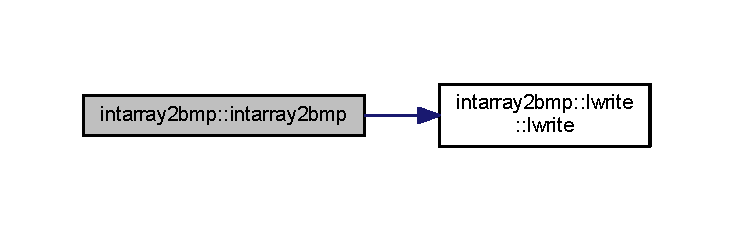
\includegraphics[width=350pt]{namespaceintarray2bmp_a504dc3b703d9a772b4d6bf1017234f49_cgraph}
\end{center}
\end{figure}




这是这个函数的调用关系图\+:
\nopagebreak
\begin{figure}[H]
\begin{center}
\leavevmode
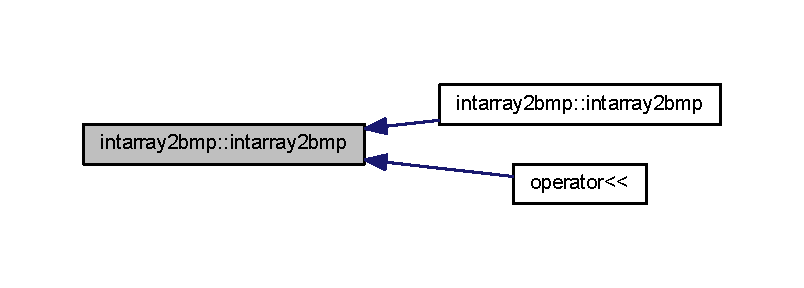
\includegraphics[width=350pt]{namespaceintarray2bmp_a504dc3b703d9a772b4d6bf1017234f49_icgraph}
\end{center}
\end{figure}


\index{intarray2bmp@{intarray2bmp}!intarray2bmp@{intarray2bmp}}
\index{intarray2bmp@{intarray2bmp}!intarray2bmp@{intarray2bmp}}
\subsubsection[{\texorpdfstring{intarray2bmp(const std\+::string \&filename, Int\+Type $\ast$intarray, unsigned rows, unsigned columns, Int\+Type min\+\_\+value, Int\+Type max\+\_\+value)}{intarray2bmp(const std::string &filename, IntType *intarray, unsigned rows, unsigned columns, IntType min_value, IntType max_value)}}]{\setlength{\rightskip}{0pt plus 5cm}template$<$typename Int\+Type $>$ bool intarray2bmp\+::intarray2bmp (
\begin{DoxyParamCaption}
\item[{const std\+::string \&}]{filename, }
\item[{Int\+Type $\ast$}]{intarray, }
\item[{unsigned}]{rows, }
\item[{unsigned}]{columns, }
\item[{Int\+Type}]{min\+\_\+value, }
\item[{Int\+Type}]{max\+\_\+value}
\end{DoxyParamCaption}
)}\hypertarget{namespaceintarray2bmp_af95c6110f71199e05a9997b17957da22}{}\label{namespaceintarray2bmp_af95c6110f71199e05a9997b17957da22}


在文件 Int\+Array2bmp.\+h 第 174 行定义.



参考 intarray2bmp().


\begin{DoxyCode}
181       \{
182     IntType** ia = \textcolor{keyword}{new}( std::nothrow ) IntType* [ rows ];
183     \textcolor{keywordflow}{for} (\textcolor{keywordtype}{unsigned} row = 0; row < rows; row++)
184       \{
185       ia[ row ] = intarray + (row * columns);
186       \}
187     \textcolor{keywordtype}{bool} result = \hyperlink{namespaceintarray2bmp_af95c6110f71199e05a9997b17957da22}{intarray2bmp}(
188                     filename, ia, rows, columns, min\_value, max\_value
189                     );
190     \textcolor{keyword}{delete} [] ia;
191     \textcolor{keywordflow}{return} result;
192     \}
\end{DoxyCode}


函数调用图\+:
\nopagebreak
\begin{figure}[H]
\begin{center}
\leavevmode
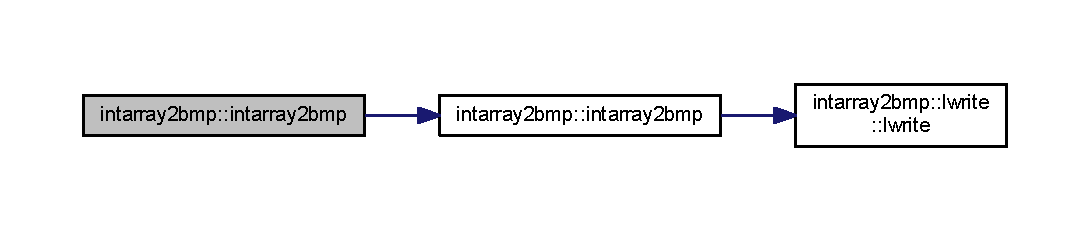
\includegraphics[width=350pt]{namespaceintarray2bmp_af95c6110f71199e05a9997b17957da22_cgraph}
\end{center}
\end{figure}


\index{intarray2bmp@{intarray2bmp}!operator$<$$<$@{operator$<$$<$}}
\index{operator$<$$<$@{operator$<$$<$}!intarray2bmp@{intarray2bmp}}
\subsubsection[{\texorpdfstring{operator$<$$<$(std\+::ostream \&outs, const lwrite \&v)}{operator<<(std::ostream &outs, const lwrite &v)}}]{\setlength{\rightskip}{0pt plus 5cm}std\+::ostream\& intarray2bmp\+::operator$<$$<$ (
\begin{DoxyParamCaption}
\item[{std\+::ostream \&}]{outs, }
\item[{const {\bf lwrite} \&}]{v}
\end{DoxyParamCaption}
)\hspace{0.3cm}{\ttfamily [inline]}}\hypertarget{namespaceintarray2bmp_a427bc6d7c8a53613eff03c28fce442ba}{}\label{namespaceintarray2bmp_a427bc6d7c8a53613eff03c28fce442ba}


在文件 Int\+Array2bmp.\+h 第 54 行定义.



参考 intarray2bmp\+::lwrite\+::size , 以及 intarray2bmp\+::lwrite\+::value.


\begin{DoxyCode}
55     \{
56     \textcolor{keywordtype}{unsigned} \textcolor{keywordtype}{long} value = v.value;
57     \textcolor{keywordflow}{for} (\textcolor{keywordtype}{unsigned} cntr = 0; cntr < v.size; cntr++, value >>= 8)
58       outs.put( static\_cast <char> (value & 0xFF) );
59     \textcolor{keywordflow}{return} outs;
60     \}
\end{DoxyCode}

\chapter{类说明}
\hypertarget{struct__GRBsvec}{}\section{\+\_\+\+G\+R\+Bsvec结构体 参考}
\label{struct__GRBsvec}\index{\+\_\+\+G\+R\+Bsvec@{\+\_\+\+G\+R\+Bsvec}}


{\ttfamily \#include \char`\"{}gurobi\+\_\+c.\+h\char`\"{}}



\+\_\+\+G\+R\+Bsvec 的协作图\+:
\nopagebreak
\begin{figure}[H]
\begin{center}
\leavevmode
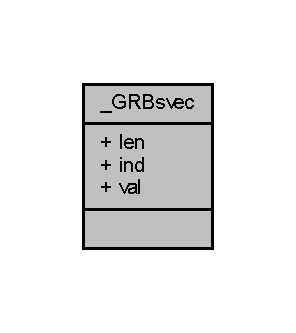
\includegraphics[width=142pt]{struct__GRBsvec__coll__graph}
\end{center}
\end{figure}
\subsection*{Public 属性}
\begin{DoxyCompactItemize}
\item 
int \hyperlink{struct__GRBsvec_a66e2892be214468f89d8512430a14428}{len}
\item 
int $\ast$ \hyperlink{struct__GRBsvec_a4a00220bb01e90ee6ce1f79b26a60095}{ind}
\item 
double $\ast$ \hyperlink{struct__GRBsvec_abb0d4946d18c0bcb33a0e132cb470c01}{val}
\end{DoxyCompactItemize}


\subsection{详细描述}


在文件 gurobi\+\_\+c.\+h 第 665 行定义.



\subsection{类成员变量说明}
\index{\+\_\+\+G\+R\+Bsvec@{\+\_\+\+G\+R\+Bsvec}!ind@{ind}}
\index{ind@{ind}!\+\_\+\+G\+R\+Bsvec@{\+\_\+\+G\+R\+Bsvec}}
\subsubsection[{\texorpdfstring{ind}{ind}}]{\setlength{\rightskip}{0pt plus 5cm}int$\ast$ \+\_\+\+G\+R\+Bsvec\+::ind}\hypertarget{struct__GRBsvec_a4a00220bb01e90ee6ce1f79b26a60095}{}\label{struct__GRBsvec_a4a00220bb01e90ee6ce1f79b26a60095}


在文件 gurobi\+\_\+c.\+h 第 668 行定义.

\index{\+\_\+\+G\+R\+Bsvec@{\+\_\+\+G\+R\+Bsvec}!len@{len}}
\index{len@{len}!\+\_\+\+G\+R\+Bsvec@{\+\_\+\+G\+R\+Bsvec}}
\subsubsection[{\texorpdfstring{len}{len}}]{\setlength{\rightskip}{0pt plus 5cm}int \+\_\+\+G\+R\+Bsvec\+::len}\hypertarget{struct__GRBsvec_a66e2892be214468f89d8512430a14428}{}\label{struct__GRBsvec_a66e2892be214468f89d8512430a14428}


在文件 gurobi\+\_\+c.\+h 第 667 行定义.

\index{\+\_\+\+G\+R\+Bsvec@{\+\_\+\+G\+R\+Bsvec}!val@{val}}
\index{val@{val}!\+\_\+\+G\+R\+Bsvec@{\+\_\+\+G\+R\+Bsvec}}
\subsubsection[{\texorpdfstring{val}{val}}]{\setlength{\rightskip}{0pt plus 5cm}double$\ast$ \+\_\+\+G\+R\+Bsvec\+::val}\hypertarget{struct__GRBsvec_abb0d4946d18c0bcb33a0e132cb470c01}{}\label{struct__GRBsvec_abb0d4946d18c0bcb33a0e132cb470c01}


在文件 gurobi\+\_\+c.\+h 第 669 行定义.



该结构体的文档由以下文件生成\+:\begin{DoxyCompactItemize}
\item 
include/\hyperlink{gurobi__c_8h}{gurobi\+\_\+c.\+h}\end{DoxyCompactItemize}

\hypertarget{classBitMatrix}{}\section{Bit\+Matrix类 参考}
\label{classBitMatrix}\index{Bit\+Matrix@{Bit\+Matrix}}


{\ttfamily \#include \char`\"{}Bit\+Matrix.\+h\char`\"{}}



Bit\+Matrix 的协作图\+:
\nopagebreak
\begin{figure}[H]
\begin{center}
\leavevmode
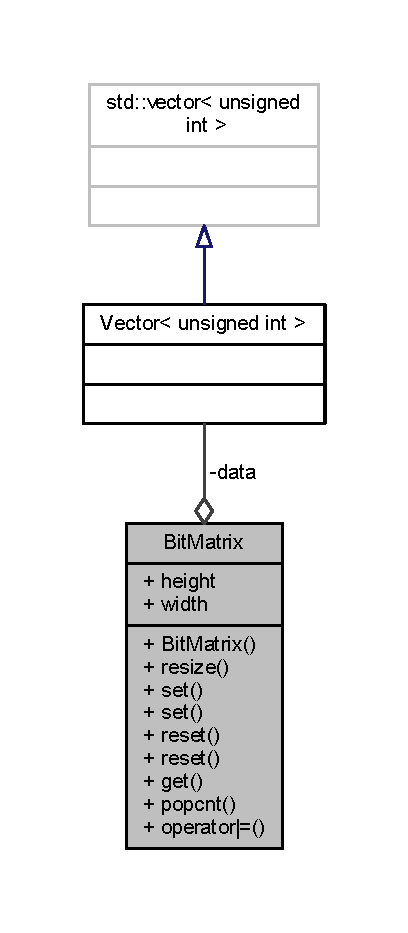
\includegraphics[width=196pt]{classBitMatrix__coll__graph}
\end{center}
\end{figure}
\subsection*{Public 成员函数}
\begin{DoxyCompactItemize}
\item 
\hyperlink{classBitMatrix_ab15c012d5aa86228f2cf19e758fed178}{Bit\+Matrix} (int h=0, int w=0)
\item 
void \hyperlink{classBitMatrix_ab09face4935598cf90705d6e8f8d1cfa}{resize} (int h, int w)
\item 
void \hyperlink{classBitMatrix_ad26dd2e93e9d24d70834d6d79e29c81e}{set} (int x, int \hyperlink{classes_8txt_a52673b1e0cce0104e52dcd12727f211e}{y})
\item 
void \hyperlink{classBitMatrix_a8ac0c3b78a28101d75a26f3d7ad43d24}{set} (\hyperlink{classPoint}{Point} point)
\item 
void \hyperlink{classBitMatrix_a0ee870454e6343c3272ab791e45af404}{reset} (int x, int \hyperlink{classes_8txt_a52673b1e0cce0104e52dcd12727f211e}{y})
\item 
void \hyperlink{classBitMatrix_acfcf5e573a47dd45c47040d96774faa0}{reset} (\hyperlink{classPoint}{Point} point)
\item 
bool \hyperlink{classBitMatrix_ad19d1045b54ccc8a99d70d38305b4ca6}{get} (int x, int \hyperlink{classes_8txt_a52673b1e0cce0104e52dcd12727f211e}{y}) const 
\item 
int \hyperlink{classBitMatrix_aff2c100f5123e0f821a1d6c6d20daf21}{popcnt} () const 
\item 
\hyperlink{classBitMatrix}{Bit\+Matrix} \& \hyperlink{classBitMatrix_ae5aeab0b906b1e70fdc2086bb434dd85}{operator$\vert$=} (const \hyperlink{classBitMatrix}{Bit\+Matrix} \&other)
\end{DoxyCompactItemize}
\subsection*{Public 属性}
\begin{DoxyCompactItemize}
\item 
int \hyperlink{classBitMatrix_a3b7a1be96313cacfd3b2a08661dd919c}{height}
\item 
int \hyperlink{classBitMatrix_ac271de23ac5446a0a75ee457a385d882}{width}
\end{DoxyCompactItemize}
\subsection*{Private 属性}
\begin{DoxyCompactItemize}
\item 
\hyperlink{classVector}{Vector}$<$ unsigned int $>$ \hyperlink{classBitMatrix_a8a914444d9945c79a7e3cc88a49ef928}{data}
\end{DoxyCompactItemize}
\subsection*{友元}
\begin{DoxyCompactItemize}
\item 
\hyperlink{global_8h_a4fcce0eedf9be71754b55a7e7a6d7f50}{O\+Stream} \& \hyperlink{classBitMatrix_ab6451c309fb63e3ef335e931f5918834}{operator$<$$<$} (\hyperlink{global_8h_a4fcce0eedf9be71754b55a7e7a6d7f50}{O\+Stream} \&ost, const \hyperlink{classBitMatrix}{Bit\+Matrix} \&bmx)
\item 
bool \hyperlink{classBitMatrix_af1c93f67e106dfcba871486f3a5c3312}{operator==} (const \hyperlink{classBitMatrix}{Bit\+Matrix} \&lhs, const \hyperlink{classBitMatrix}{Bit\+Matrix} \&rhs)
\item 
bool \hyperlink{classBitMatrix_a57e43b3edc6cb3a9d083d4bf6af9045c}{operator$<$} (const \hyperlink{classBitMatrix}{Bit\+Matrix} \&lhs, const \hyperlink{classBitMatrix}{Bit\+Matrix} \&rhs)
\item 
bool \hyperlink{classBitMatrix_a61fcfe2623514f269a51fd57d199c66a}{operator!=} (const \hyperlink{classBitMatrix}{Bit\+Matrix} \&lhs, const \hyperlink{classBitMatrix}{Bit\+Matrix} \&rhs)
\end{DoxyCompactItemize}


\subsection{详细描述}


在文件 Bit\+Matrix.\+h 第 6 行定义.



\subsection{构造及析构函数说明}
\index{Bit\+Matrix@{Bit\+Matrix}!Bit\+Matrix@{Bit\+Matrix}}
\index{Bit\+Matrix@{Bit\+Matrix}!Bit\+Matrix@{Bit\+Matrix}}
\subsubsection[{\texorpdfstring{Bit\+Matrix(int h=0, int w=0)}{BitMatrix(int h=0, int w=0)}}]{\setlength{\rightskip}{0pt plus 5cm}Bit\+Matrix\+::\+Bit\+Matrix (
\begin{DoxyParamCaption}
\item[{int}]{h = {\ttfamily 0}, }
\item[{int}]{w = {\ttfamily 0}}
\end{DoxyParamCaption}
)\hspace{0.3cm}{\ttfamily [inline]}}\hypertarget{classBitMatrix_ab15c012d5aa86228f2cf19e758fed178}{}\label{classBitMatrix_ab15c012d5aa86228f2cf19e758fed178}


在文件 Bit\+Matrix.\+h 第 12 行定义.



参考 resize().


\begin{DoxyCode}
13     \{
14         \hyperlink{classBitMatrix_ab09face4935598cf90705d6e8f8d1cfa}{resize}(h, w);
15     \}
\end{DoxyCode}


函数调用图\+:
\nopagebreak
\begin{figure}[H]
\begin{center}
\leavevmode
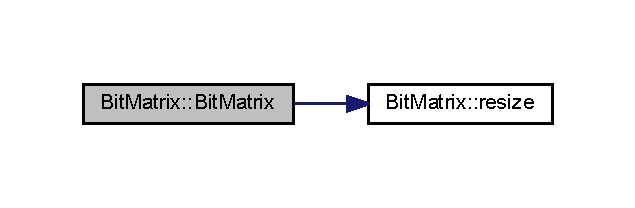
\includegraphics[width=305pt]{classBitMatrix_ab15c012d5aa86228f2cf19e758fed178_cgraph}
\end{center}
\end{figure}




\subsection{成员函数说明}
\index{Bit\+Matrix@{Bit\+Matrix}!get@{get}}
\index{get@{get}!Bit\+Matrix@{Bit\+Matrix}}
\subsubsection[{\texorpdfstring{get(int x, int y) const }{get(int x, int y) const }}]{\setlength{\rightskip}{0pt plus 5cm}bool Bit\+Matrix\+::get (
\begin{DoxyParamCaption}
\item[{int}]{x, }
\item[{int}]{y}
\end{DoxyParamCaption}
) const\hspace{0.3cm}{\ttfamily [inline]}}\hypertarget{classBitMatrix_ad19d1045b54ccc8a99d70d38305b4ca6}{}\label{classBitMatrix_ad19d1045b54ccc8a99d70d38305b4ca6}


在文件 Bit\+Matrix.\+h 第 39 行定义.



参考 operator!=, operator$<$, operator$<$$<$, operator==, operator$\vert$=(), popcnt() , 以及 y.



参考自 Clever\+Optimize\+::bfs(), Column\+Gen\+Solve\+::dfs\+Edge(), Clever\+Optimize\+::get\+Map(), operator$<$$<$(), Column\+Gen\+Solve\+::par\+Dijkstra(), Column\+Gen\+Solve\+::remove\+Non\+Cuts(), Column\+Gen\+Solve\+::suggest\+Tree(), Column\+Gen\+Solve\+::tree\+Branches(), Column\+Gen\+Solve\+::tree\+D\+F\+S\+Branches(), Column\+Gen\+Solve\+::tree\+D\+F\+S\+Get\+Branches() , 以及 Column\+Gen\+Solve\+::tree\+Get\+Branches().


\begin{DoxyCode}
40     \{
41         x = x * \hyperlink{classBitMatrix_ac271de23ac5446a0a75ee457a385d882}{width} + \hyperlink{classes_8txt_a52673b1e0cce0104e52dcd12727f211e}{y};
42         \textcolor{keywordflow}{return} \hyperlink{classBitMatrix_a8a914444d9945c79a7e3cc88a49ef928}{data}[x >> 5] >> (x & 31) & 1;
43     \}
\end{DoxyCode}


函数调用图\+:
\nopagebreak
\begin{figure}[H]
\begin{center}
\leavevmode
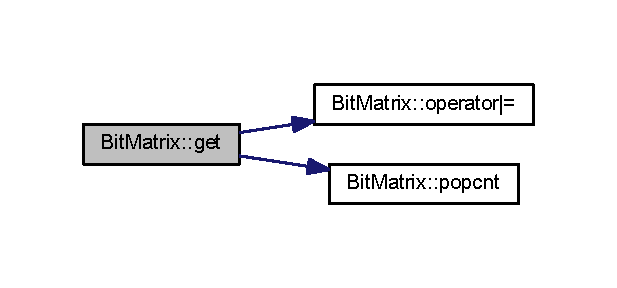
\includegraphics[width=296pt]{classBitMatrix_ad19d1045b54ccc8a99d70d38305b4ca6_cgraph}
\end{center}
\end{figure}




这是这个函数的调用关系图\+:
\nopagebreak
\begin{figure}[H]
\begin{center}
\leavevmode
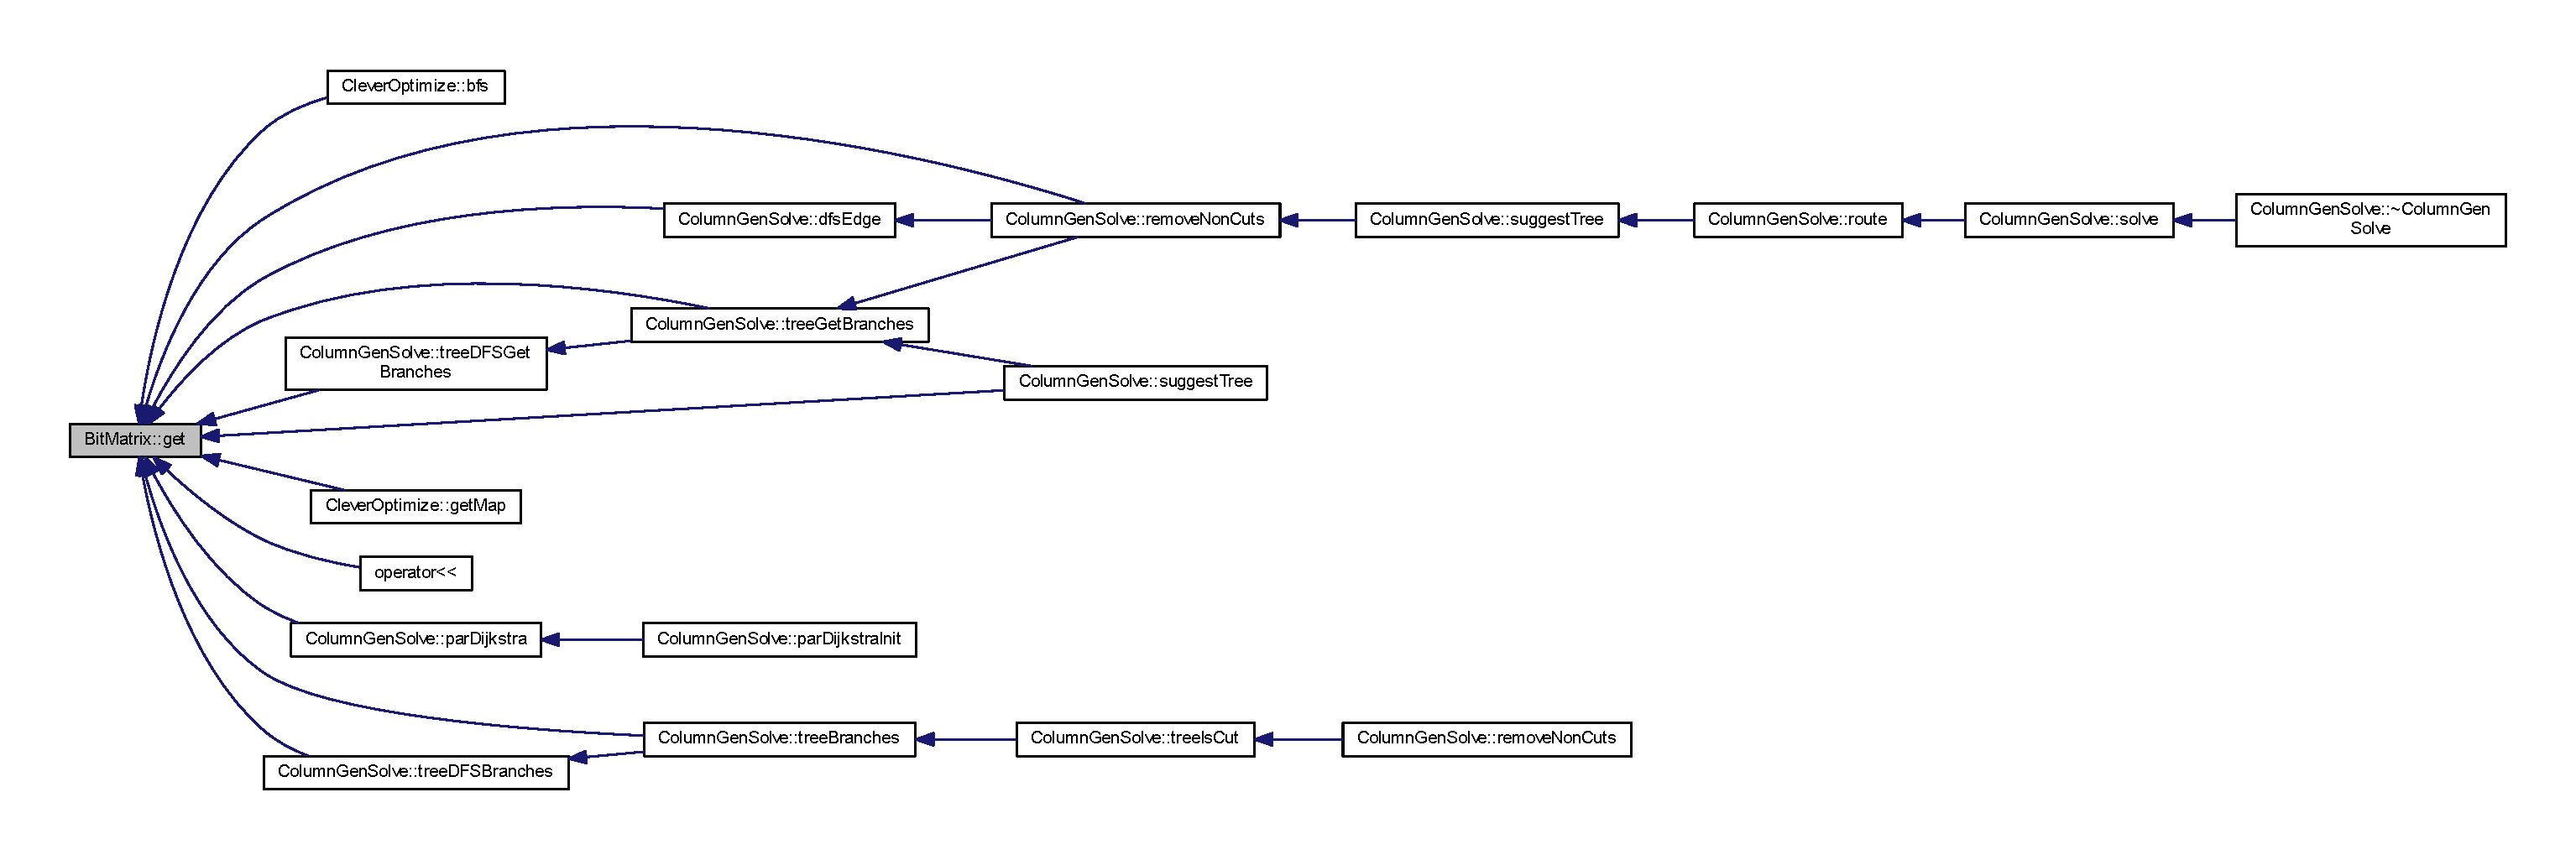
\includegraphics[width=350pt]{classBitMatrix_ad19d1045b54ccc8a99d70d38305b4ca6_icgraph}
\end{center}
\end{figure}


\index{Bit\+Matrix@{Bit\+Matrix}!operator\texttt{"|}=@{operator\texttt{"|}=}}
\index{operator\texttt{"|}=@{operator\texttt{"|}=}!Bit\+Matrix@{Bit\+Matrix}}
\subsubsection[{\texorpdfstring{operator\texttt{"|}=(const Bit\+Matrix \&other)}{operator|=(const BitMatrix &other)}}]{\setlength{\rightskip}{0pt plus 5cm}{\bf Bit\+Matrix} \& Bit\+Matrix\+::operator$\vert$= (
\begin{DoxyParamCaption}
\item[{const {\bf Bit\+Matrix} \&}]{other}
\end{DoxyParamCaption}
)}\hypertarget{classBitMatrix_ae5aeab0b906b1e70fdc2086bb434dd85}{}\label{classBitMatrix_ae5aeab0b906b1e70fdc2086bb434dd85}


在文件 Bit\+Matrix.\+cpp 第 46 行定义.



参考 assert, data, height , 以及 width.



参考自 get().


\begin{DoxyCode}
47 \{
48     \hyperlink{global_8h_af576bf8ffa22a44e53018c67095ffbf0}{assert}(\hyperlink{classBitMatrix_a3b7a1be96313cacfd3b2a08661dd919c}{height} == other.\hyperlink{classBitMatrix_a3b7a1be96313cacfd3b2a08661dd919c}{height});
49     \hyperlink{global_8h_af576bf8ffa22a44e53018c67095ffbf0}{assert}(\hyperlink{classBitMatrix_ac271de23ac5446a0a75ee457a385d882}{width} == other.\hyperlink{classBitMatrix_ac271de23ac5446a0a75ee457a385d882}{width});
50     \textcolor{keywordtype}{int} tot = (\hyperlink{classBitMatrix_a3b7a1be96313cacfd3b2a08661dd919c}{height} * \hyperlink{classBitMatrix_ac271de23ac5446a0a75ee457a385d882}{width} + 31) >> 5;
51     \textcolor{keywordtype}{unsigned} *cur = &\hyperlink{classBitMatrix_a8a914444d9945c79a7e3cc88a49ef928}{data}[0];
52     \textcolor{keyword}{const} \textcolor{keywordtype}{unsigned} *oth = &other.\hyperlink{classBitMatrix_a8a914444d9945c79a7e3cc88a49ef928}{data}[0];
53     \textcolor{keywordflow}{for}(\textcolor{keywordtype}{int} i = 0; i < tot; i++)
54         cur[i] |= oth[i];
55     \textcolor{keywordflow}{return} *\textcolor{keyword}{this};
56 \}
\end{DoxyCode}


这是这个函数的调用关系图\+:
\nopagebreak
\begin{figure}[H]
\begin{center}
\leavevmode
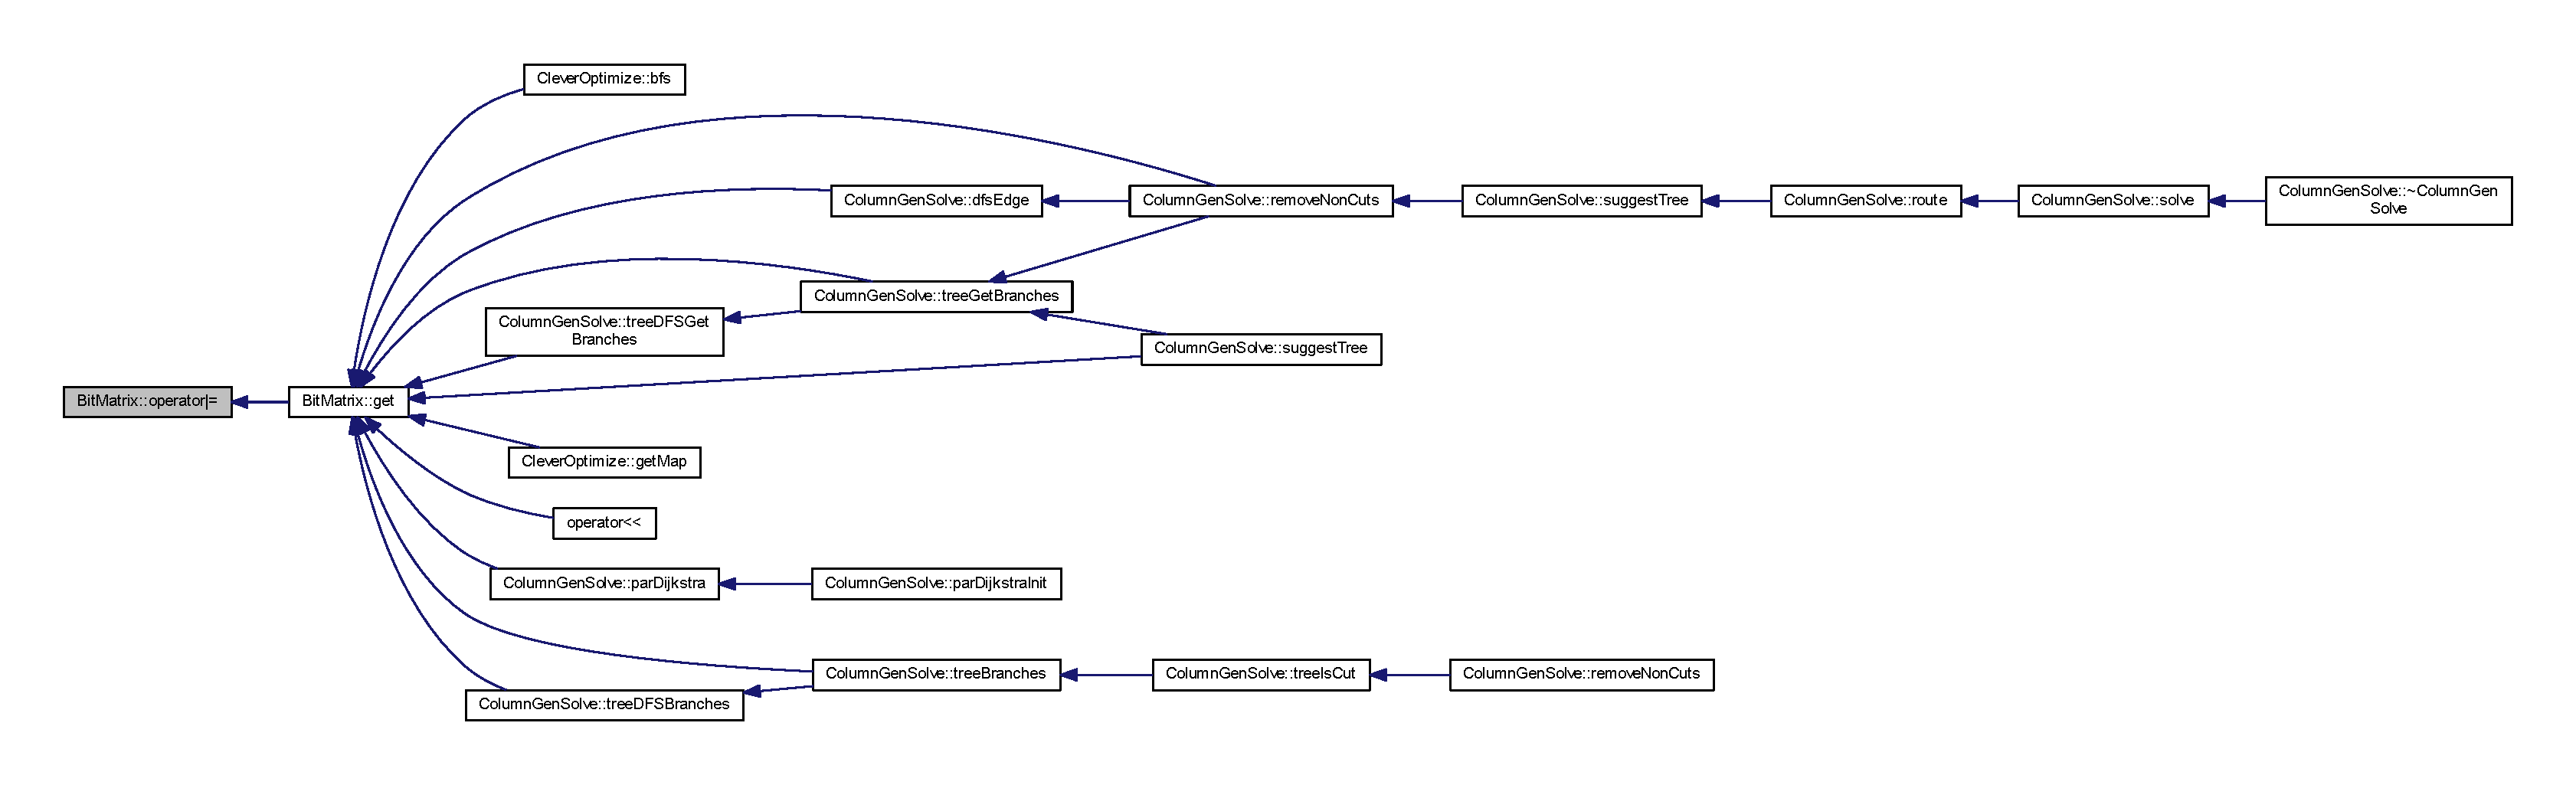
\includegraphics[width=350pt]{classBitMatrix_ae5aeab0b906b1e70fdc2086bb434dd85_icgraph}
\end{center}
\end{figure}


\index{Bit\+Matrix@{Bit\+Matrix}!popcnt@{popcnt}}
\index{popcnt@{popcnt}!Bit\+Matrix@{Bit\+Matrix}}
\subsubsection[{\texorpdfstring{popcnt() const }{popcnt() const }}]{\setlength{\rightskip}{0pt plus 5cm}int Bit\+Matrix\+::popcnt (
\begin{DoxyParamCaption}
{}
\end{DoxyParamCaption}
) const}\hypertarget{classBitMatrix_aff2c100f5123e0f821a1d6c6d20daf21}{}\label{classBitMatrix_aff2c100f5123e0f821a1d6c6d20daf21}


在文件 Bit\+Matrix.\+cpp 第 3 行定义.



参考 height , 以及 width.



参考自 Tree\+::compute\+Length() , 以及 get().


\begin{DoxyCode}
4 \{
5     \textcolor{comment}{// TODO: can be improved}
6     \textcolor{keywordtype}{int} ans = 0;
7     \textcolor{keywordflow}{for}(\textcolor{keywordtype}{int} i = 0; i < \hyperlink{classBitMatrix_a3b7a1be96313cacfd3b2a08661dd919c}{height}; i++)
8         \textcolor{keywordflow}{for}(\textcolor{keywordtype}{int} j = 0; j < \hyperlink{classBitMatrix_ac271de23ac5446a0a75ee457a385d882}{width}; j++)
9             ans += (\textcolor{keywordtype}{int}) \textcolor{keyword}{get}(i, j);
10     \textcolor{keywordflow}{return} ans;
11 \}
\end{DoxyCode}


这是这个函数的调用关系图\+:
\nopagebreak
\begin{figure}[H]
\begin{center}
\leavevmode
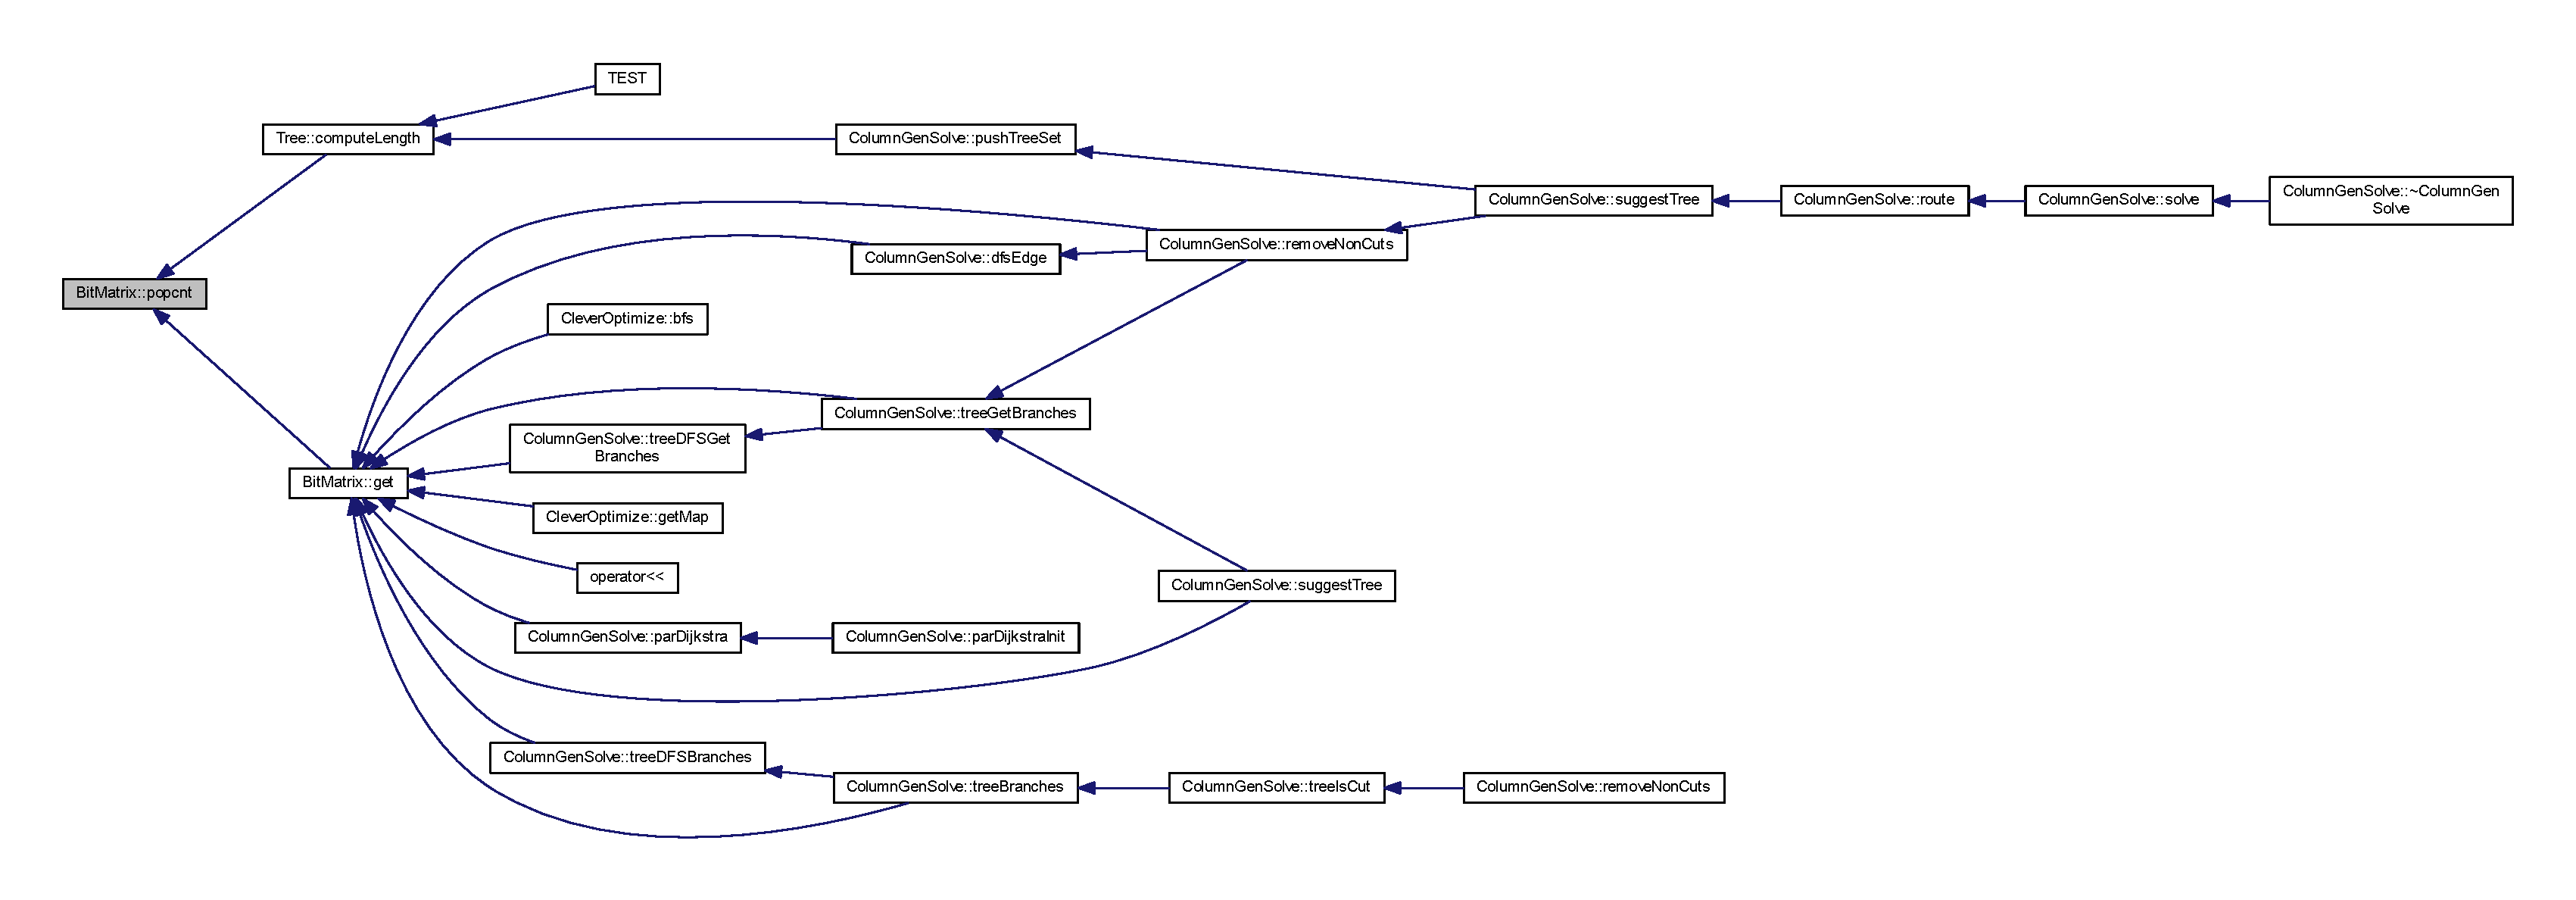
\includegraphics[width=350pt]{classBitMatrix_aff2c100f5123e0f821a1d6c6d20daf21_icgraph}
\end{center}
\end{figure}


\index{Bit\+Matrix@{Bit\+Matrix}!reset@{reset}}
\index{reset@{reset}!Bit\+Matrix@{Bit\+Matrix}}
\subsubsection[{\texorpdfstring{reset(int x, int y)}{reset(int x, int y)}}]{\setlength{\rightskip}{0pt plus 5cm}void Bit\+Matrix\+::reset (
\begin{DoxyParamCaption}
\item[{int}]{x, }
\item[{int}]{y}
\end{DoxyParamCaption}
)\hspace{0.3cm}{\ttfamily [inline]}}\hypertarget{classBitMatrix_a0ee870454e6343c3272ab791e45af404}{}\label{classBitMatrix_a0ee870454e6343c3272ab791e45af404}


在文件 Bit\+Matrix.\+h 第 30 行定义.



参考 y.



参考自 Column\+Gen\+Solve\+::dfs\+Edge(), Column\+Gen\+Solve\+::remove\+Non\+Cuts(), reset(), Column\+Gen\+Solve\+::tree\+D\+F\+S\+Branches(), Column\+Gen\+Solve\+::tree\+D\+F\+S\+Get\+Branches() , 以及 Column\+Gen\+Solve\+::tree\+Is\+Cut().


\begin{DoxyCode}
31     \{
32         x = x * \hyperlink{classBitMatrix_ac271de23ac5446a0a75ee457a385d882}{width} + \hyperlink{classes_8txt_a52673b1e0cce0104e52dcd12727f211e}{y};
33         \hyperlink{classBitMatrix_a8a914444d9945c79a7e3cc88a49ef928}{data}[x >> 5] &= ~(1u << (x & 31));
34     \}
\end{DoxyCode}


这是这个函数的调用关系图\+:
\nopagebreak
\begin{figure}[H]
\begin{center}
\leavevmode
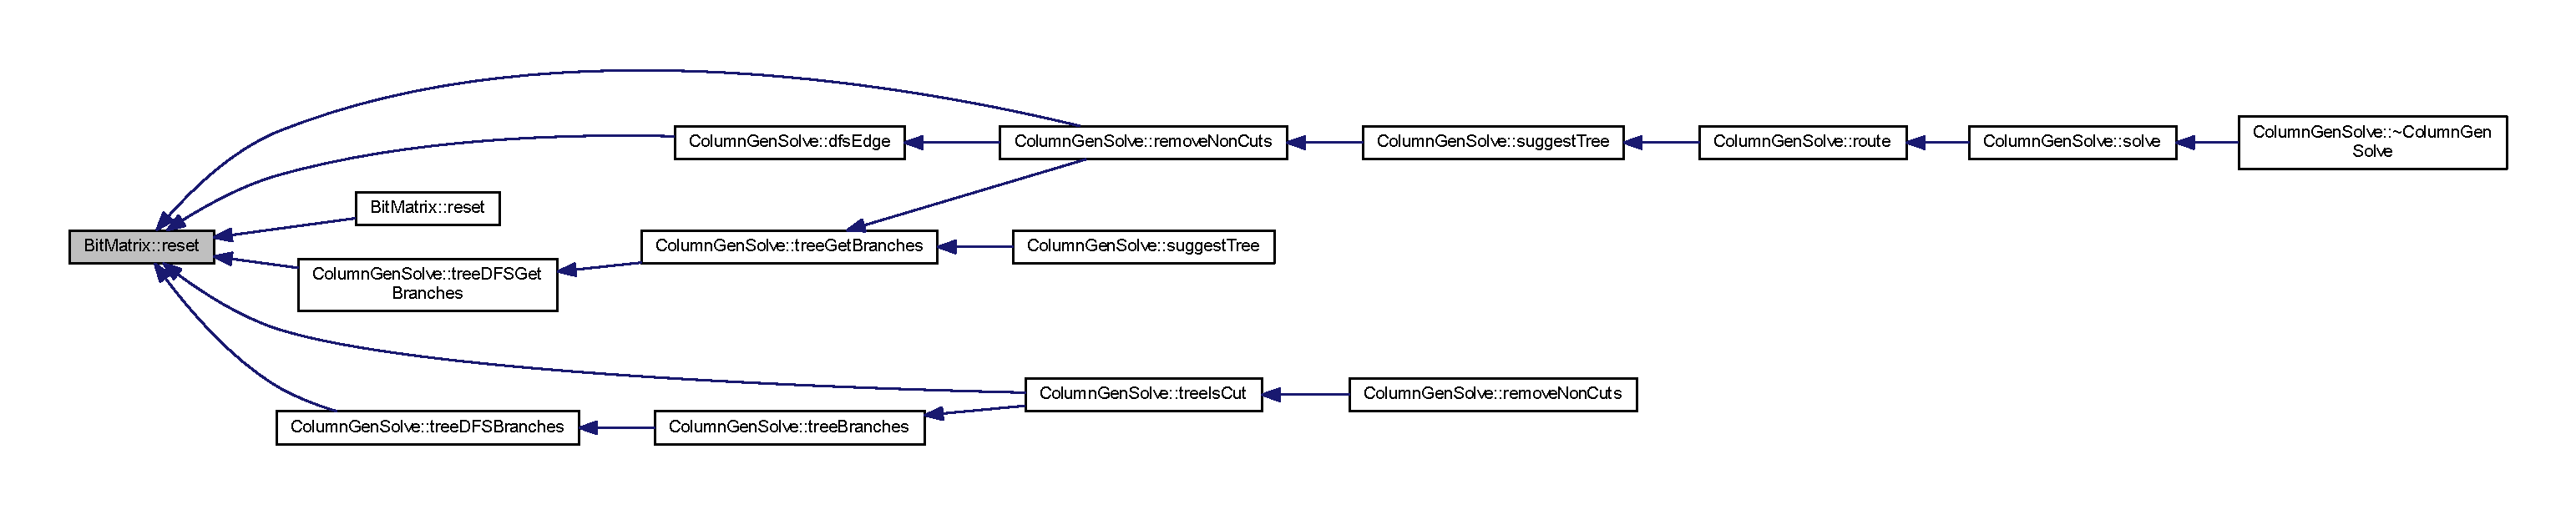
\includegraphics[width=350pt]{classBitMatrix_a0ee870454e6343c3272ab791e45af404_icgraph}
\end{center}
\end{figure}


\index{Bit\+Matrix@{Bit\+Matrix}!reset@{reset}}
\index{reset@{reset}!Bit\+Matrix@{Bit\+Matrix}}
\subsubsection[{\texorpdfstring{reset(\+Point point)}{reset(Point point)}}]{\setlength{\rightskip}{0pt plus 5cm}void Bit\+Matrix\+::reset (
\begin{DoxyParamCaption}
\item[{{\bf Point}}]{point}
\end{DoxyParamCaption}
)\hspace{0.3cm}{\ttfamily [inline]}}\hypertarget{classBitMatrix_acfcf5e573a47dd45c47040d96774faa0}{}\label{classBitMatrix_acfcf5e573a47dd45c47040d96774faa0}


在文件 Bit\+Matrix.\+h 第 35 行定义.



参考 reset(), Point\+::x , 以及 Point\+::y.


\begin{DoxyCode}
36     \{
37         \hyperlink{classBitMatrix_a0ee870454e6343c3272ab791e45af404}{reset}(point.\hyperlink{classPoint_a8c779e11e694b20e0946105a9f5de842}{x}, point.\hyperlink{classPoint_a2e1b5fb2b2a83571f5c0bc0f66a73cf7}{y});
38     \}
\end{DoxyCode}


函数调用图\+:
\nopagebreak
\begin{figure}[H]
\begin{center}
\leavevmode
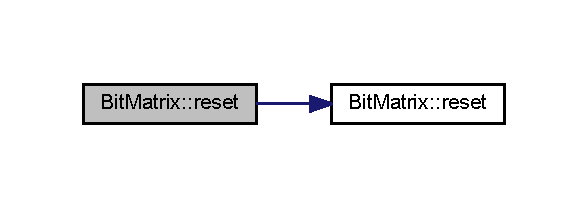
\includegraphics[width=282pt]{classBitMatrix_acfcf5e573a47dd45c47040d96774faa0_cgraph}
\end{center}
\end{figure}


\index{Bit\+Matrix@{Bit\+Matrix}!resize@{resize}}
\index{resize@{resize}!Bit\+Matrix@{Bit\+Matrix}}
\subsubsection[{\texorpdfstring{resize(int h, int w)}{resize(int h, int w)}}]{\setlength{\rightskip}{0pt plus 5cm}void Bit\+Matrix\+::resize (
\begin{DoxyParamCaption}
\item[{int}]{h, }
\item[{int}]{w}
\end{DoxyParamCaption}
)\hspace{0.3cm}{\ttfamily [inline]}}\hypertarget{classBitMatrix_ab09face4935598cf90705d6e8f8d1cfa}{}\label{classBitMatrix_ab09face4935598cf90705d6e8f8d1cfa}


在文件 Bit\+Matrix.\+h 第 16 行定义.



参考自 Bit\+Matrix(), Column\+Gen\+Solve\+::suggest\+Tree(), Tree\+::\+Tree() , 以及 Column\+Gen\+Solve\+::tree\+Get\+Branches().


\begin{DoxyCode}
17     \{
18         \hyperlink{classBitMatrix_a3b7a1be96313cacfd3b2a08661dd919c}{height} = h; \hyperlink{classBitMatrix_ac271de23ac5446a0a75ee457a385d882}{width} = w;
19         \hyperlink{classBitMatrix_a8a914444d9945c79a7e3cc88a49ef928}{data}.resize((h * w + 31) >> 5);
20     \}
\end{DoxyCode}


这是这个函数的调用关系图\+:
\nopagebreak
\begin{figure}[H]
\begin{center}
\leavevmode
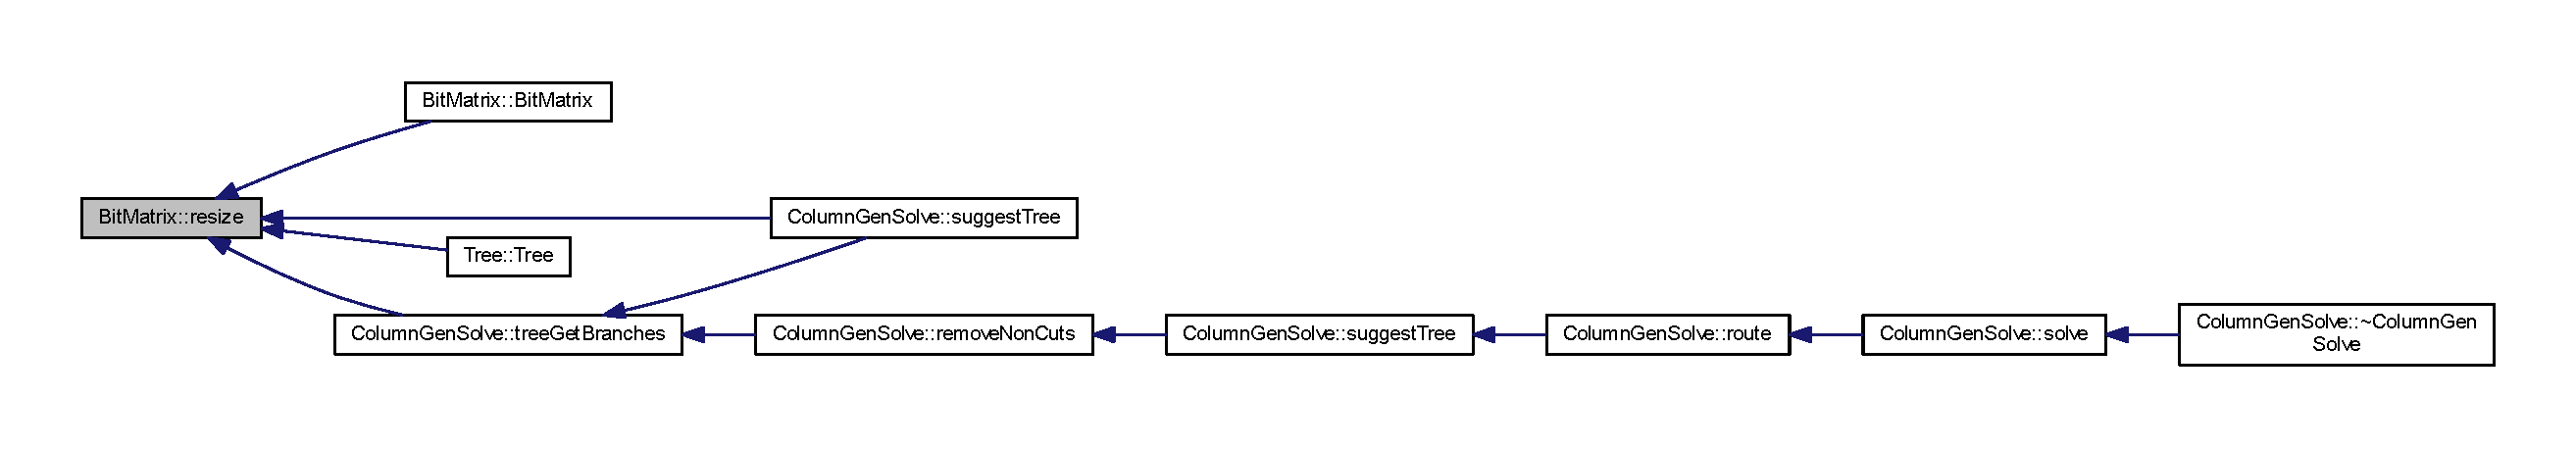
\includegraphics[width=350pt]{classBitMatrix_ab09face4935598cf90705d6e8f8d1cfa_icgraph}
\end{center}
\end{figure}


\index{Bit\+Matrix@{Bit\+Matrix}!set@{set}}
\index{set@{set}!Bit\+Matrix@{Bit\+Matrix}}
\subsubsection[{\texorpdfstring{set(int x, int y)}{set(int x, int y)}}]{\setlength{\rightskip}{0pt plus 5cm}void Bit\+Matrix\+::set (
\begin{DoxyParamCaption}
\item[{int}]{x, }
\item[{int}]{y}
\end{DoxyParamCaption}
)\hspace{0.3cm}{\ttfamily [inline]}}\hypertarget{classBitMatrix_ad26dd2e93e9d24d70834d6d79e29c81e}{}\label{classBitMatrix_ad26dd2e93e9d24d70834d6d79e29c81e}


在文件 Bit\+Matrix.\+h 第 21 行定义.



参考 y.



参考自 Clever\+Optimize\+::backtrace(), Bit\+Matrix\+Test(), Clever\+Optimize\+::get\+Map(), Column\+Gen\+Solve\+::remove\+Non\+Cuts(), Column\+Gen\+Solve\+::suggest\+Tree(), T\+E\+S\+T() , 以及 Column\+Gen\+Solve\+::tree\+D\+F\+S\+Get\+Branches().


\begin{DoxyCode}
22     \{
23         x = x * \hyperlink{classBitMatrix_ac271de23ac5446a0a75ee457a385d882}{width} + \hyperlink{classes_8txt_a52673b1e0cce0104e52dcd12727f211e}{y};
24         \hyperlink{classBitMatrix_a8a914444d9945c79a7e3cc88a49ef928}{data}[x >> 5] |= (1u << (x & 31));
25     \}
\end{DoxyCode}


这是这个函数的调用关系图\+:
\nopagebreak
\begin{figure}[H]
\begin{center}
\leavevmode
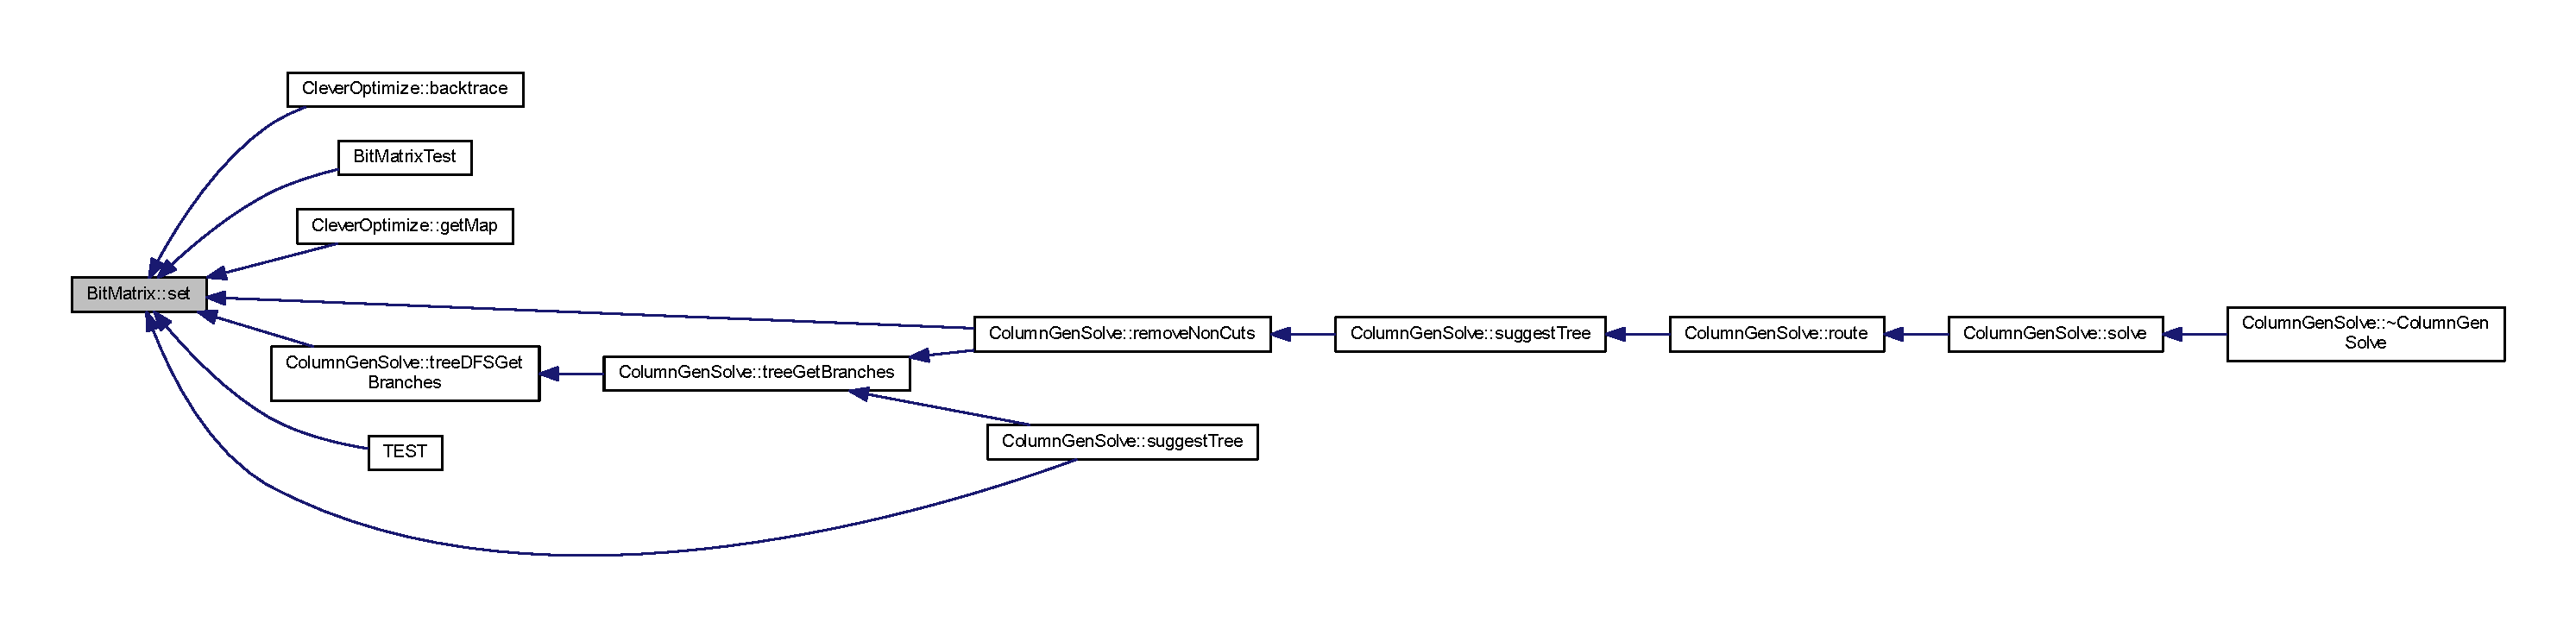
\includegraphics[width=350pt]{classBitMatrix_ad26dd2e93e9d24d70834d6d79e29c81e_icgraph}
\end{center}
\end{figure}


\index{Bit\+Matrix@{Bit\+Matrix}!set@{set}}
\index{set@{set}!Bit\+Matrix@{Bit\+Matrix}}
\subsubsection[{\texorpdfstring{set(\+Point point)}{set(Point point)}}]{\setlength{\rightskip}{0pt plus 5cm}void Bit\+Matrix\+::set (
\begin{DoxyParamCaption}
\item[{{\bf Point}}]{point}
\end{DoxyParamCaption}
)\hspace{0.3cm}{\ttfamily [inline]}}\hypertarget{classBitMatrix_a8ac0c3b78a28101d75a26f3d7ad43d24}{}\label{classBitMatrix_a8ac0c3b78a28101d75a26f3d7ad43d24}


在文件 Bit\+Matrix.\+h 第 26 行定义.


\begin{DoxyCode}
27     \{
28         \textcolor{keyword}{set}(point.\hyperlink{classPoint_a8c779e11e694b20e0946105a9f5de842}{x}, point.\hyperlink{classPoint_a2e1b5fb2b2a83571f5c0bc0f66a73cf7}{y});
29     \}
\end{DoxyCode}


\subsection{友元及相关函数文档}
\index{Bit\+Matrix@{Bit\+Matrix}!operator"!=@{operator"!=}}
\index{operator"!=@{operator"!=}!Bit\+Matrix@{Bit\+Matrix}}
\subsubsection[{\texorpdfstring{operator"!=}{operator!=}}]{\setlength{\rightskip}{0pt plus 5cm}bool operator!= (
\begin{DoxyParamCaption}
\item[{const {\bf Bit\+Matrix} \&}]{lhs, }
\item[{const {\bf Bit\+Matrix} \&}]{rhs}
\end{DoxyParamCaption}
)\hspace{0.3cm}{\ttfamily [friend]}}\hypertarget{classBitMatrix_a61fcfe2623514f269a51fd57d199c66a}{}\label{classBitMatrix_a61fcfe2623514f269a51fd57d199c66a}


在文件 Bit\+Matrix.\+cpp 第 41 行定义.



参考自 get().


\begin{DoxyCode}
42 \{
43     \textcolor{keywordflow}{return} !(lhs == rhs);
44 \}
\end{DoxyCode}
\index{Bit\+Matrix@{Bit\+Matrix}!operator$<$@{operator$<$}}
\index{operator$<$@{operator$<$}!Bit\+Matrix@{Bit\+Matrix}}
\subsubsection[{\texorpdfstring{operator$<$}{operator<}}]{\setlength{\rightskip}{0pt plus 5cm}bool operator$<$ (
\begin{DoxyParamCaption}
\item[{const {\bf Bit\+Matrix} \&}]{lhs, }
\item[{const {\bf Bit\+Matrix} \&}]{rhs}
\end{DoxyParamCaption}
)\hspace{0.3cm}{\ttfamily [friend]}}\hypertarget{classBitMatrix_a57e43b3edc6cb3a9d083d4bf6af9045c}{}\label{classBitMatrix_a57e43b3edc6cb3a9d083d4bf6af9045c}


在文件 Bit\+Matrix.\+cpp 第 33 行定义.



参考自 get().


\begin{DoxyCode}
34 \{
35     \textcolor{keywordtype}{int} sz = lhs.\hyperlink{classBitMatrix_a3b7a1be96313cacfd3b2a08661dd919c}{height} * lhs.\hyperlink{classBitMatrix_ac271de23ac5446a0a75ee457a385d882}{width};
36     \textcolor{keywordflow}{if}(sz != rhs.\hyperlink{classBitMatrix_a3b7a1be96313cacfd3b2a08661dd919c}{height} * rhs.\hyperlink{classBitMatrix_ac271de23ac5446a0a75ee457a385d882}{width})
37         \textcolor{keywordflow}{return} sz < rhs.\hyperlink{classBitMatrix_a3b7a1be96313cacfd3b2a08661dd919c}{height} * rhs.\hyperlink{classBitMatrix_ac271de23ac5446a0a75ee457a385d882}{width};
38     \textcolor{keywordflow}{return} lhs.\hyperlink{classBitMatrix_a8a914444d9945c79a7e3cc88a49ef928}{data} < rhs.\hyperlink{classBitMatrix_a8a914444d9945c79a7e3cc88a49ef928}{data};
39 \}
\end{DoxyCode}
\index{Bit\+Matrix@{Bit\+Matrix}!operator$<$$<$@{operator$<$$<$}}
\index{operator$<$$<$@{operator$<$$<$}!Bit\+Matrix@{Bit\+Matrix}}
\subsubsection[{\texorpdfstring{operator$<$$<$}{operator<<}}]{\setlength{\rightskip}{0pt plus 5cm}{\bf O\+Stream}\& operator$<$$<$ (
\begin{DoxyParamCaption}
\item[{{\bf O\+Stream} \&}]{ost, }
\item[{const {\bf Bit\+Matrix} \&}]{bmx}
\end{DoxyParamCaption}
)\hspace{0.3cm}{\ttfamily [friend]}}\hypertarget{classBitMatrix_ab6451c309fb63e3ef335e931f5918834}{}\label{classBitMatrix_ab6451c309fb63e3ef335e931f5918834}


在文件 Bit\+Matrix.\+cpp 第 13 行定义.



参考自 get().


\begin{DoxyCode}
14 \{
15     ost << \textcolor{stringliteral}{"BitMatrix "} << bmx.\hyperlink{classBitMatrix_a3b7a1be96313cacfd3b2a08661dd919c}{height} << \textcolor{stringliteral}{" * "} << bmx.\hyperlink{classBitMatrix_ac271de23ac5446a0a75ee457a385d882}{width} << \textcolor{stringliteral}{"\(\backslash\)n"};
16     \textcolor{keywordflow}{for}(\textcolor{keywordtype}{int} i = 0; i < bmx.\hyperlink{classBitMatrix_a3b7a1be96313cacfd3b2a08661dd919c}{height}; i++)
17     \{
18         \textcolor{keywordflow}{for}(\textcolor{keywordtype}{int} j = 0; j < bmx.\hyperlink{classBitMatrix_ac271de23ac5446a0a75ee457a385d882}{width}; j++)
19             ost << (\textcolor{keywordtype}{int}) bmx.\hyperlink{classBitMatrix_ad19d1045b54ccc8a99d70d38305b4ca6}{get}(i, j);
20         ost << \textcolor{stringliteral}{"\(\backslash\)n"};
21     \}
22     \textcolor{keywordflow}{return} ost;
23 \}
\end{DoxyCode}
\index{Bit\+Matrix@{Bit\+Matrix}!operator==@{operator==}}
\index{operator==@{operator==}!Bit\+Matrix@{Bit\+Matrix}}
\subsubsection[{\texorpdfstring{operator==}{operator==}}]{\setlength{\rightskip}{0pt plus 5cm}bool operator== (
\begin{DoxyParamCaption}
\item[{const {\bf Bit\+Matrix} \&}]{lhs, }
\item[{const {\bf Bit\+Matrix} \&}]{rhs}
\end{DoxyParamCaption}
)\hspace{0.3cm}{\ttfamily [friend]}}\hypertarget{classBitMatrix_af1c93f67e106dfcba871486f3a5c3312}{}\label{classBitMatrix_af1c93f67e106dfcba871486f3a5c3312}


在文件 Bit\+Matrix.\+cpp 第 25 行定义.



参考自 get().


\begin{DoxyCode}
26 \{
27     \textcolor{keywordtype}{int} sz = lhs.\hyperlink{classBitMatrix_a3b7a1be96313cacfd3b2a08661dd919c}{height} * lhs.\hyperlink{classBitMatrix_ac271de23ac5446a0a75ee457a385d882}{width};
28     \textcolor{keywordflow}{if}(sz != rhs.\hyperlink{classBitMatrix_a3b7a1be96313cacfd3b2a08661dd919c}{height} * rhs.\hyperlink{classBitMatrix_ac271de23ac5446a0a75ee457a385d882}{width})
29         \textcolor{keywordflow}{return} \textcolor{keyword}{false};
30     \textcolor{keywordflow}{return} lhs.\hyperlink{classBitMatrix_a8a914444d9945c79a7e3cc88a49ef928}{data} == rhs.\hyperlink{classBitMatrix_a8a914444d9945c79a7e3cc88a49ef928}{data};
31 \}
\end{DoxyCode}


\subsection{类成员变量说明}
\index{Bit\+Matrix@{Bit\+Matrix}!data@{data}}
\index{data@{data}!Bit\+Matrix@{Bit\+Matrix}}
\subsubsection[{\texorpdfstring{data}{data}}]{\setlength{\rightskip}{0pt plus 5cm}{\bf Vector}$<$unsigned int$>$ Bit\+Matrix\+::data\hspace{0.3cm}{\ttfamily [private]}}\hypertarget{classBitMatrix_a8a914444d9945c79a7e3cc88a49ef928}{}\label{classBitMatrix_a8a914444d9945c79a7e3cc88a49ef928}


在文件 Bit\+Matrix.\+h 第 9 行定义.



参考自 operator$<$(), operator==() , 以及 operator$\vert$=().

\index{Bit\+Matrix@{Bit\+Matrix}!height@{height}}
\index{height@{height}!Bit\+Matrix@{Bit\+Matrix}}
\subsubsection[{\texorpdfstring{height}{height}}]{\setlength{\rightskip}{0pt plus 5cm}int Bit\+Matrix\+::height}\hypertarget{classBitMatrix_a3b7a1be96313cacfd3b2a08661dd919c}{}\label{classBitMatrix_a3b7a1be96313cacfd3b2a08661dd919c}


在文件 Bit\+Matrix.\+h 第 11 行定义.



参考自 Clever\+Optimize\+::backtrace(), Clever\+Optimize\+::bfs(), Clever\+Optimize\+::get\+Map(), operator$<$(), operator$<$$<$(), operator==(), operator$\vert$=() , 以及 popcnt().

\index{Bit\+Matrix@{Bit\+Matrix}!width@{width}}
\index{width@{width}!Bit\+Matrix@{Bit\+Matrix}}
\subsubsection[{\texorpdfstring{width}{width}}]{\setlength{\rightskip}{0pt plus 5cm}int Bit\+Matrix\+::width}\hypertarget{classBitMatrix_ac271de23ac5446a0a75ee457a385d882}{}\label{classBitMatrix_ac271de23ac5446a0a75ee457a385d882}


在文件 Bit\+Matrix.\+h 第 11 行定义.



参考自 Clever\+Optimize\+::bfs(), Clever\+Optimize\+::get\+Map(), operator$<$(), operator$<$$<$(), operator==(), operator$\vert$=() , 以及 popcnt().



该类的文档由以下文件生成\+:\begin{DoxyCompactItemize}
\item 
include/\hyperlink{BitMatrix_8h}{Bit\+Matrix.\+h}\item 
src/\hyperlink{BitMatrix_8cpp}{Bit\+Matrix.\+cpp}\end{DoxyCompactItemize}

\hypertarget{classBoard}{}\section{Board类 参考}
\label{classBoard}\index{Board@{Board}}


{\ttfamily \#include \char`\"{}Board.\+h\char`\"{}}



Board 的协作图\+:
\nopagebreak
\begin{figure}[H]
\begin{center}
\leavevmode
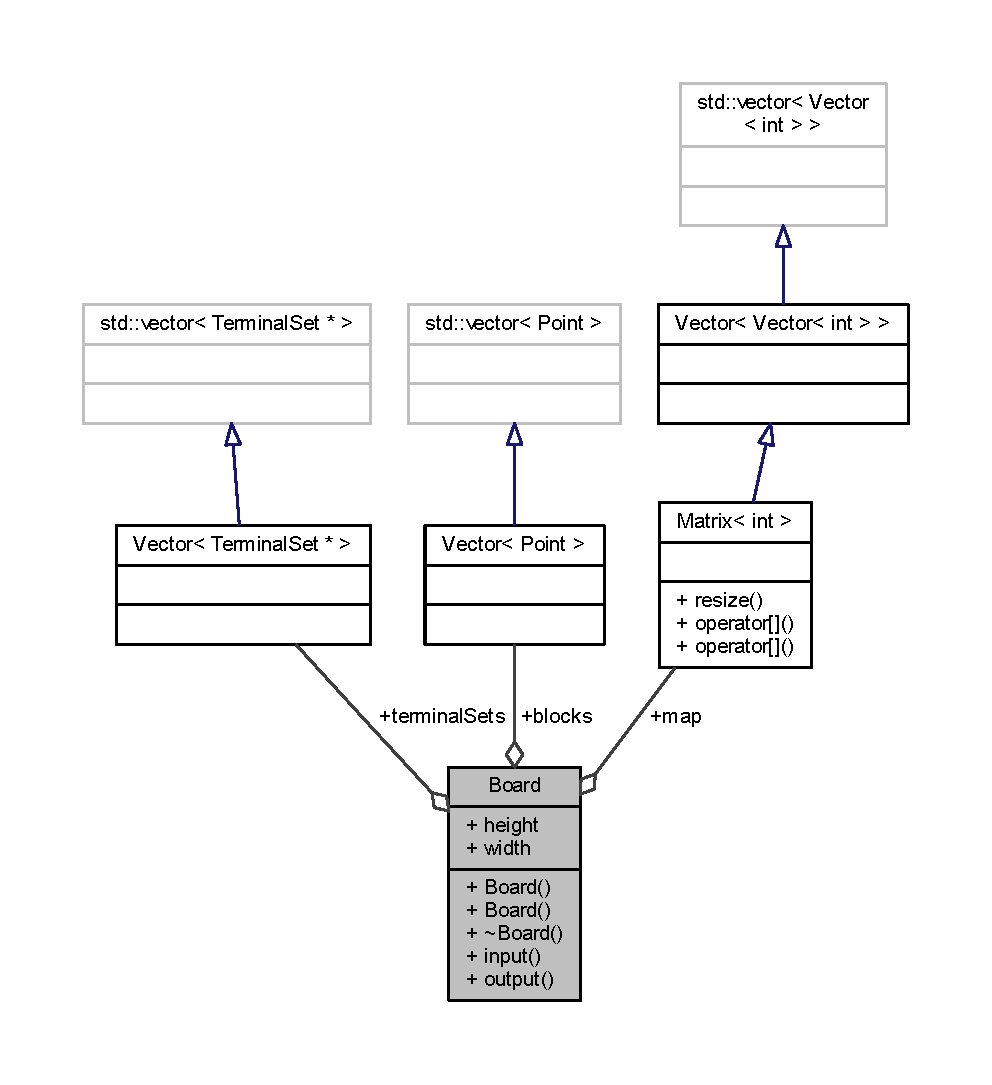
\includegraphics[width=350pt]{classBoard__coll__graph}
\end{center}
\end{figure}
\subsection*{Public 成员函数}
\begin{DoxyCompactItemize}
\item 
\hyperlink{classBoard_a9ee491d4fea680cf69b033374a9fdfcb}{Board} ()
\item 
\hyperlink{classBoard_a19e2c1f6c2baf8ab04cbd02f0cd2aebc}{Board} (const \hyperlink{classBoard}{Board} \&)
\item 
\hyperlink{classBoard_af73f45730119a1fd8f6670f53f959e68}{$\sim$\+Board} ()
\item 
void \hyperlink{classBoard_ace215dfac6b741c9fb51cc40a6fe6ab1}{input} (int mode=0, \hyperlink{global_8h_a3ae955d826788591b03995dc737012c7}{I\+Stream} \&ifs=cin)
\item 
void \hyperlink{classBoard_a88190948cb3ed605cb54355de513cfa6}{output} (int mode=0, \hyperlink{global_8h_a4fcce0eedf9be71754b55a7e7a6d7f50}{O\+Stream} \&ofs=cout) const 
\end{DoxyCompactItemize}
\subsection*{Public 属性}
\begin{DoxyCompactItemize}
\item 
int \hyperlink{classBoard_aa0cb8de0254520dc08dab5796643c8e5}{height}
\item 
int \hyperlink{classBoard_a90a8efaa4736af25511ac948bdd27d6c}{width}
\item 
\hyperlink{classVector}{Vector}$<$ \hyperlink{classTerminalSet}{Terminal\+Set} $\ast$ $>$ \hyperlink{classBoard_a6683a9c042af7113f55c5bc1b9656b69}{terminal\+Sets}
\item 
\hyperlink{classMatrix}{Matrix}$<$ int $>$ \hyperlink{classBoard_a191ff45df9151b8fee0c32877f582165}{map}
\item 
\hyperlink{classVector}{Vector}$<$ \hyperlink{classPoint}{Point} $>$ \hyperlink{classBoard_abd553dee0125b79f672dbfa74f86c52b}{blocks}
\end{DoxyCompactItemize}


\subsection{详细描述}


在文件 Board.\+h 第 7 行定义.



\subsection{构造及析构函数说明}
\index{Board@{Board}!Board@{Board}}
\index{Board@{Board}!Board@{Board}}
\subsubsection[{\texorpdfstring{Board()}{Board()}}]{\setlength{\rightskip}{0pt plus 5cm}Board\+::\+Board (
\begin{DoxyParamCaption}
{}
\end{DoxyParamCaption}
)\hspace{0.3cm}{\ttfamily [inline]}}\hypertarget{classBoard_a9ee491d4fea680cf69b033374a9fdfcb}{}\label{classBoard_a9ee491d4fea680cf69b033374a9fdfcb}


在文件 Board.\+h 第 10 行定义.


\begin{DoxyCode}
10 \{\}
\end{DoxyCode}
\index{Board@{Board}!Board@{Board}}
\index{Board@{Board}!Board@{Board}}
\subsubsection[{\texorpdfstring{Board(const Board \&)}{Board(const Board &)}}]{\setlength{\rightskip}{0pt plus 5cm}Board\+::\+Board (
\begin{DoxyParamCaption}
\item[{const {\bf Board} \&}]{\+\_\+board}
\end{DoxyParamCaption}
)}\hypertarget{classBoard_a19e2c1f6c2baf8ab04cbd02f0cd2aebc}{}\label{classBoard_a19e2c1f6c2baf8ab04cbd02f0cd2aebc}


在文件 Board.\+cpp 第 10 行定义.



参考 Terminal\+Set\+::\+Add\+Point(), blocks, height, map, terminal\+Sets , 以及 width.


\begin{DoxyCode}
11 \{
12     this->\hyperlink{classBoard_aa0cb8de0254520dc08dab5796643c8e5}{height} = \_board.\hyperlink{classBoard_aa0cb8de0254520dc08dab5796643c8e5}{height};
13     this->\hyperlink{classBoard_a90a8efaa4736af25511ac948bdd27d6c}{width} = \_board.\hyperlink{classBoard_a90a8efaa4736af25511ac948bdd27d6c}{width};
14     this->\hyperlink{classBoard_a191ff45df9151b8fee0c32877f582165}{map} = \_board.\hyperlink{classBoard_a191ff45df9151b8fee0c32877f582165}{map};
15     this->\hyperlink{classBoard_abd553dee0125b79f672dbfa74f86c52b}{blocks} = \_board.\hyperlink{classBoard_abd553dee0125b79f672dbfa74f86c52b}{blocks};
16     \textcolor{keywordflow}{for} (\textcolor{keywordtype}{unsigned} \textcolor{keywordtype}{int} i = 0;i < \_board.\hyperlink{classBoard_a6683a9c042af7113f55c5bc1b9656b69}{terminalSets}.size();++i)
17         \textcolor{keywordflow}{if} (\_board.\hyperlink{classBoard_a6683a9c042af7113f55c5bc1b9656b69}{terminalSets}[i] == NULL)
18             this->\hyperlink{classBoard_a6683a9c042af7113f55c5bc1b9656b69}{terminalSets}.push\_back(NULL);
19         \textcolor{keywordflow}{else}
20         \{
21             \hyperlink{classTerminalSet}{TerminalSet}* temp = \textcolor{keyword}{new} \hyperlink{classTerminalSet}{TerminalSet}(\_board.
      \hyperlink{classBoard_a6683a9c042af7113f55c5bc1b9656b69}{terminalSets}[i]->id,\textcolor{keyword}{this});
22             \textcolor{keywordflow}{for} (\textcolor{keywordtype}{unsigned} \textcolor{keywordtype}{int} j = 0;j < \_board.\hyperlink{classBoard_a6683a9c042af7113f55c5bc1b9656b69}{terminalSets}[i]->points.size();++j)
23                 temp->\hyperlink{classTerminalSet_a405cff3b74573b5459da6ffd387f347a}{AddPoint}(\_board.\hyperlink{classBoard_a6683a9c042af7113f55c5bc1b9656b69}{terminalSets}[i]->points[j]);
24             this->\hyperlink{classBoard_a6683a9c042af7113f55c5bc1b9656b69}{terminalSets}.push\_back(temp);
25         \}
26             
27 \}
\end{DoxyCode}


函数调用图\+:
\nopagebreak
\begin{figure}[H]
\begin{center}
\leavevmode
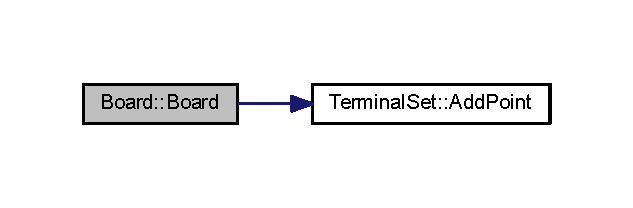
\includegraphics[width=304pt]{classBoard_a19e2c1f6c2baf8ab04cbd02f0cd2aebc_cgraph}
\end{center}
\end{figure}


\index{Board@{Board}!````~Board@{$\sim$\+Board}}
\index{````~Board@{$\sim$\+Board}!Board@{Board}}
\subsubsection[{\texorpdfstring{$\sim$\+Board()}{~Board()}}]{\setlength{\rightskip}{0pt plus 5cm}Board\+::$\sim$\+Board (
\begin{DoxyParamCaption}
{}
\end{DoxyParamCaption}
)}\hypertarget{classBoard_af73f45730119a1fd8f6670f53f959e68}{}\label{classBoard_af73f45730119a1fd8f6670f53f959e68}


在文件 Board.\+cpp 第 4 行定义.



参考 terminal\+Sets.


\begin{DoxyCode}
5 \{
6     \textcolor{keywordflow}{for}(\textcolor{keyword}{auto} pointer: \hyperlink{classBoard_a6683a9c042af7113f55c5bc1b9656b69}{terminalSets})
7         \textcolor{keyword}{delete} pointer;
8 \}
\end{DoxyCode}


\subsection{成员函数说明}
\index{Board@{Board}!input@{input}}
\index{input@{input}!Board@{Board}}
\subsubsection[{\texorpdfstring{input(int mode=0, I\+Stream \&ifs=cin)}{input(int mode=0, IStream &ifs=cin)}}]{\setlength{\rightskip}{0pt plus 5cm}void Board\+::input (
\begin{DoxyParamCaption}
\item[{int}]{mode = {\ttfamily 0}, }
\item[{{\bf I\+Stream} \&}]{ifs = {\ttfamily cin}}
\end{DoxyParamCaption}
)}\hypertarget{classBoard_ace215dfac6b741c9fb51cc40a6fe6ab1}{}\label{classBoard_ace215dfac6b741c9fb51cc40a6fe6ab1}


在文件 Board.\+cpp 第 29 行定义.



参考 Terminal\+Set\+::\+Add\+Point(), blocks, height, id, map, Matrix$<$ T $>$\+::resize(), terminal\+Sets, width , 以及 y.



参考自 Board\+I\+O\+Test(), D\+A\+C\+Solve\+::divide(), Large\+Test(), D\+A\+C\+Solve\+::solve(), Stupid\+Strategy\+Test() , 以及 T\+E\+S\+T().


\begin{DoxyCode}
30 \{
31     \textcolor{keywordflow}{if} (mode == 0)
32     \{
33         \textcolor{comment}{//input the size of the board}
34         ifs>>\hyperlink{classBoard_aa0cb8de0254520dc08dab5796643c8e5}{height}>>\hyperlink{classBoard_a90a8efaa4736af25511ac948bdd27d6c}{width};
35         \hyperlink{classBoard_a191ff45df9151b8fee0c32877f582165}{map}.\hyperlink{classMatrix_a15ce96c8af4c7a982c2c10b96f29cea1}{resize}(\hyperlink{classBoard_aa0cb8de0254520dc08dab5796643c8e5}{height},width);
36         \textcolor{comment}{//input every element of the board}
37         \textcolor{keywordtype}{int} maxindex = 0;
38         \textcolor{keywordflow}{for} (\textcolor{keywordtype}{int} i = 0;i < \hyperlink{classBoard_aa0cb8de0254520dc08dab5796643c8e5}{height}; ++i)
39             \textcolor{keywordflow}{for} (\textcolor{keywordtype}{int} j = 0; j < \hyperlink{classBoard_a90a8efaa4736af25511ac948bdd27d6c}{width}; ++j)
40             \{
41                 ifs>>\hyperlink{classBoard_a191ff45df9151b8fee0c32877f582165}{map}[i][j];
42                 maxindex = max(maxindex,map[i][j]);
43             \}
44     \hyperlink{classBoard_a6683a9c042af7113f55c5bc1b9656b69}{terminalSets}.resize(maxindex+1);
45     \textcolor{keywordflow}{for} (\textcolor{keywordtype}{int} i = 0;i < (int)\hyperlink{classBoard_a6683a9c042af7113f55c5bc1b9656b69}{terminalSets}.size(); ++i)
46         \hyperlink{classBoard_a6683a9c042af7113f55c5bc1b9656b69}{terminalSets}[i] = \textcolor{keyword}{new} \hyperlink{classTerminalSet}{TerminalSet}(i,\textcolor{keyword}{this});
47     \textcolor{keywordflow}{for} (\textcolor{keywordtype}{int} i = 0;i < \hyperlink{classBoard_aa0cb8de0254520dc08dab5796643c8e5}{height}; ++i)
48         \textcolor{keywordflow}{for} (\textcolor{keywordtype}{int} j = 0; j < \hyperlink{classBoard_a90a8efaa4736af25511ac948bdd27d6c}{width}; ++j)
49         \{
50             \textcolor{keywordflow}{if} (\hyperlink{classBoard_a191ff45df9151b8fee0c32877f582165}{map}[i][j] == -1) \hyperlink{classBoard_abd553dee0125b79f672dbfa74f86c52b}{blocks}.push\_back(\hyperlink{classPoint}{Point}(i,j));
51             \textcolor{keywordflow}{else} \textcolor{keywordflow}{if} (\hyperlink{classBoard_a191ff45df9151b8fee0c32877f582165}{map}[i][j] > 0)
52             \hyperlink{classBoard_a6683a9c042af7113f55c5bc1b9656b69}{terminalSets}[\hyperlink{classBoard_a191ff45df9151b8fee0c32877f582165}{map}[i][j]]->AddPoint(\hyperlink{classPoint}{Point}(i,j));
53         \}   
54     \}
55     \textcolor{keywordflow}{else}
56     \{
57         \textcolor{keywordtype}{int} \hyperlink{classes_8txt_a7441ef0865bcb3db9b8064dd7375c1ea}{id};
58         ifs>>height>>\hyperlink{classBoard_a90a8efaa4736af25511ac948bdd27d6c}{width};
59         \hyperlink{classBoard_a191ff45df9151b8fee0c32877f582165}{map}.\hyperlink{classMatrix_a15ce96c8af4c7a982c2c10b96f29cea1}{resize}(height,width);
60         \hyperlink{classTerminalSet}{TerminalSet} *terminal0 = \textcolor{keyword}{new} \hyperlink{classTerminalSet}{TerminalSet}(0,\textcolor{keyword}{this});
61         \hyperlink{classBoard_a6683a9c042af7113f55c5bc1b9656b69}{terminalSets}.push\_back(terminal0);
62         \textcolor{keywordflow}{while} (ifs>>\textcolor{keywordtype}{id})
63         \{
64             \textcolor{keywordtype}{int} x,\hyperlink{classes_8txt_a52673b1e0cce0104e52dcd12727f211e}{y};
65             \textcolor{keywordtype}{int} n;
66             ifs>>n;
67             \textcolor{keywordflow}{if} (\textcolor{keywordtype}{id} > 0)
68             \{
69                 \hyperlink{classTerminalSet}{TerminalSet} *terminal = \textcolor{keyword}{new} \hyperlink{classTerminalSet}{TerminalSet}(\textcolor{keywordtype}{id},\textcolor{keyword}{this});
70                 \textcolor{keywordflow}{for} (\textcolor{keywordtype}{int} i = 1;i <= n; ++i)
71                 \{
72                     ifs>>x>>\hyperlink{classes_8txt_a52673b1e0cce0104e52dcd12727f211e}{y};
73                     terminal->\hyperlink{classTerminalSet_a405cff3b74573b5459da6ffd387f347a}{AddPoint}(\hyperlink{classPoint}{Point}(x,y));
74                     \hyperlink{classBoard_a191ff45df9151b8fee0c32877f582165}{map}[x][\hyperlink{classes_8txt_a52673b1e0cce0104e52dcd12727f211e}{y}] = \hyperlink{classes_8txt_a7441ef0865bcb3db9b8064dd7375c1ea}{id};
75                 \}
76                 \hyperlink{classBoard_a6683a9c042af7113f55c5bc1b9656b69}{terminalSets}.push\_back(terminal);
77             \}
78             \textcolor{keywordflow}{else} \textcolor{keywordflow}{if} (\textcolor{keywordtype}{id} == -1)
79             \{
80                 \textcolor{keywordflow}{for} (\textcolor{keywordtype}{int} i = 1;i <=n; ++i)
81                 \{
82                     ifs>>x>>\hyperlink{classes_8txt_a52673b1e0cce0104e52dcd12727f211e}{y};
83                     \hyperlink{classBoard_abd553dee0125b79f672dbfa74f86c52b}{blocks}.push\_back(\hyperlink{classPoint}{Point}(x,y));
84                     \hyperlink{classBoard_a191ff45df9151b8fee0c32877f582165}{map}[x][\hyperlink{classes_8txt_a52673b1e0cce0104e52dcd12727f211e}{y}] = -1;
85                 \}
86             \}
87                 
88         \}
89     \}
90 \}
\end{DoxyCode}


函数调用图\+:
\nopagebreak
\begin{figure}[H]
\begin{center}
\leavevmode
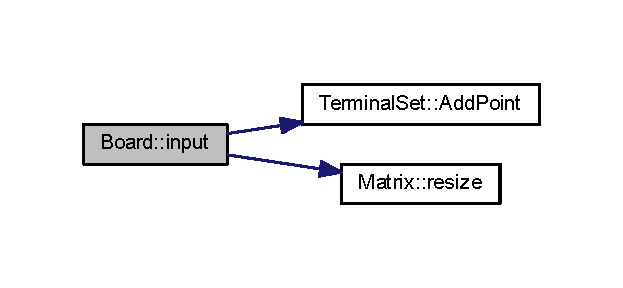
\includegraphics[width=299pt]{classBoard_ace215dfac6b741c9fb51cc40a6fe6ab1_cgraph}
\end{center}
\end{figure}




这是这个函数的调用关系图\+:
\nopagebreak
\begin{figure}[H]
\begin{center}
\leavevmode
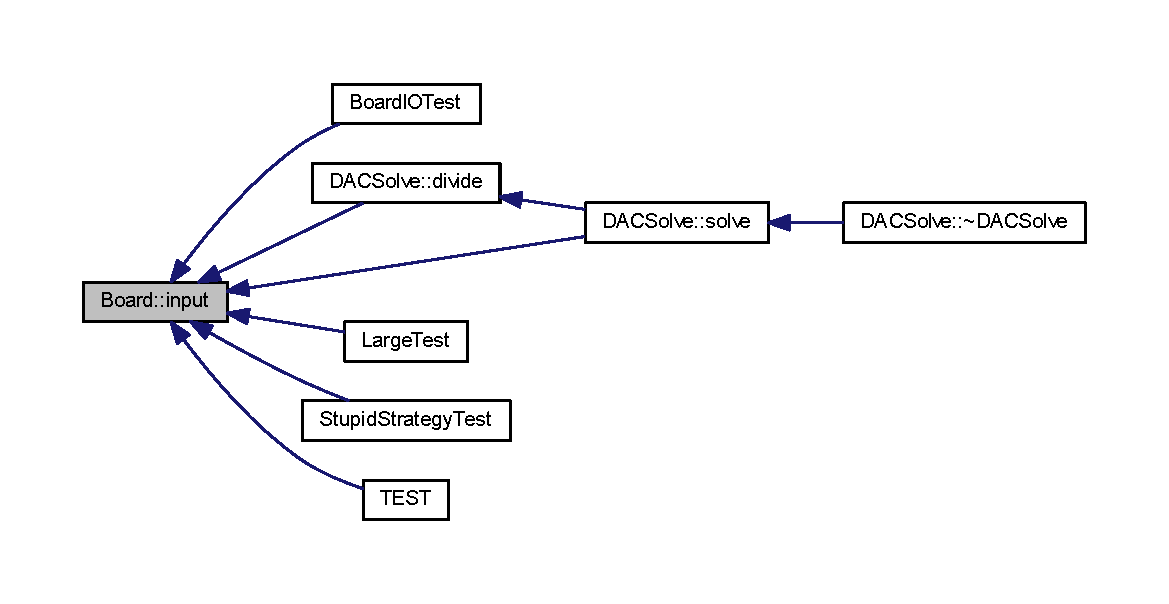
\includegraphics[width=350pt]{classBoard_ace215dfac6b741c9fb51cc40a6fe6ab1_icgraph}
\end{center}
\end{figure}


\index{Board@{Board}!output@{output}}
\index{output@{output}!Board@{Board}}
\subsubsection[{\texorpdfstring{output(int mode=0, O\+Stream \&ofs=cout) const }{output(int mode=0, OStream &ofs=cout) const }}]{\setlength{\rightskip}{0pt plus 5cm}void Board\+::output (
\begin{DoxyParamCaption}
\item[{int}]{mode = {\ttfamily 0}, }
\item[{{\bf O\+Stream} \&}]{ofs = {\ttfamily cout}}
\end{DoxyParamCaption}
) const}\hypertarget{classBoard_a88190948cb3ed605cb54355de513cfa6}{}\label{classBoard_a88190948cb3ed605cb54355de513cfa6}


在文件 Board.\+cpp 第 92 行定义.



参考 blocks, height, map, points, terminal\+Sets, width , 以及 y.



参考自 Board\+I\+O\+Test().


\begin{DoxyCode}
93 \{
94     \textcolor{keywordflow}{if} (mode == 0)
95     \{
96         ofs<<\hyperlink{classBoard_aa0cb8de0254520dc08dab5796643c8e5}{height}<<\textcolor{charliteral}{' '}<<\hyperlink{classBoard_a90a8efaa4736af25511ac948bdd27d6c}{width}<<\textcolor{charliteral}{'\(\backslash\)n'};
97         \textcolor{keywordflow}{for} (\textcolor{keywordtype}{int} i = 0;i < \hyperlink{classBoard_aa0cb8de0254520dc08dab5796643c8e5}{height}; ++i)
98         \{
99             \textcolor{keywordflow}{for} (\textcolor{keywordtype}{int} j = 0;j < \hyperlink{classBoard_a90a8efaa4736af25511ac948bdd27d6c}{width}; ++j)
100                 ofs<<\hyperlink{classBoard_a191ff45df9151b8fee0c32877f582165}{map}[i][j]<<\textcolor{charliteral}{' '};
101             ofs<<\textcolor{charliteral}{'\(\backslash\)n'};
102         \}
103     \}
104     \textcolor{keywordflow}{else}
105     \{
106         ofs<<height<<\textcolor{charliteral}{' '}<<width<<\textcolor{charliteral}{'\(\backslash\)n'};
107         \textcolor{keywordflow}{for} (\textcolor{keywordtype}{int} i = 1;i < (int)\hyperlink{classBoard_a6683a9c042af7113f55c5bc1b9656b69}{terminalSets}.size(); ++i)
108         \{
109             ofs<<i<<\textcolor{charliteral}{' '}<<\hyperlink{classBoard_a6683a9c042af7113f55c5bc1b9656b69}{terminalSets}[i]->points.size()<<\textcolor{charliteral}{'\(\backslash\)n'};
110             \textcolor{keywordflow}{for} (\textcolor{keywordtype}{int} j = 0;j < (int)\hyperlink{classBoard_a6683a9c042af7113f55c5bc1b9656b69}{terminalSets}[i]->\hyperlink{classes_8txt_ae368e6252d0add75ea011d5d90db68ed}{points}.size(); ++j)
111                 ofs<<\hyperlink{classBoard_a6683a9c042af7113f55c5bc1b9656b69}{terminalSets}[i]->\hyperlink{classes_8txt_ae368e6252d0add75ea011d5d90db68ed}{points}[j].x<<\textcolor{charliteral}{' '}<<
      \hyperlink{classBoard_a6683a9c042af7113f55c5bc1b9656b69}{terminalSets}[i]->\hyperlink{classes_8txt_ae368e6252d0add75ea011d5d90db68ed}{points}[j].\hyperlink{classes_8txt_a52673b1e0cce0104e52dcd12727f211e}{y}<<\textcolor{charliteral}{' '}<<\textcolor{charliteral}{'\(\backslash\)n'};
112         \}
113         ofs<<-1<<\textcolor{charliteral}{' '}<<\hyperlink{classBoard_abd553dee0125b79f672dbfa74f86c52b}{blocks}.size()<<\textcolor{charliteral}{'\(\backslash\)n'};
114         \textcolor{keywordflow}{for} (\textcolor{keywordtype}{int} i = 0;i < (int)\hyperlink{classBoard_abd553dee0125b79f672dbfa74f86c52b}{blocks}.size(); ++i)
115             ofs<<\hyperlink{classBoard_abd553dee0125b79f672dbfa74f86c52b}{blocks}[i].x<<\textcolor{charliteral}{' '}<<\hyperlink{classBoard_abd553dee0125b79f672dbfa74f86c52b}{blocks}[i].\hyperlink{classes_8txt_a52673b1e0cce0104e52dcd12727f211e}{y}<<\textcolor{charliteral}{'\(\backslash\)n'};
116     \}
117 \}\end{DoxyCode}


这是这个函数的调用关系图\+:
\nopagebreak
\begin{figure}[H]
\begin{center}
\leavevmode
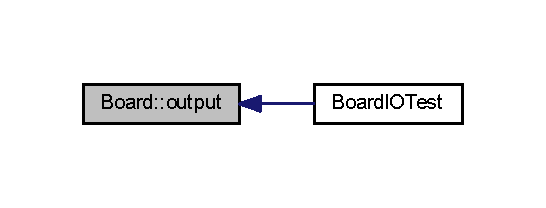
\includegraphics[width=262pt]{classBoard_a88190948cb3ed605cb54355de513cfa6_icgraph}
\end{center}
\end{figure}




\subsection{类成员变量说明}
\index{Board@{Board}!blocks@{blocks}}
\index{blocks@{blocks}!Board@{Board}}
\subsubsection[{\texorpdfstring{blocks}{blocks}}]{\setlength{\rightskip}{0pt plus 5cm}{\bf Vector}$<${\bf Point}$>$ Board\+::blocks}\hypertarget{classBoard_abd553dee0125b79f672dbfa74f86c52b}{}\label{classBoard_abd553dee0125b79f672dbfa74f86c52b}


在文件 Board.\+h 第 15 行定义.



参考自 Board(), Solution\+::compute\+Map(), input() , 以及 output().

\index{Board@{Board}!height@{height}}
\index{height@{height}!Board@{Board}}
\subsubsection[{\texorpdfstring{height}{height}}]{\setlength{\rightskip}{0pt plus 5cm}int Board\+::height}\hypertarget{classBoard_aa0cb8de0254520dc08dab5796643c8e5}{}\label{classBoard_aa0cb8de0254520dc08dab5796643c8e5}


在文件 Board.\+h 第 11 行定义.



参考自 Board(), Solution\+::compute\+Map(), input(), operator$<$$<$(), output(), Column\+Gen\+Solve\+::route(), Column\+Gen\+Solve\+::solve(), D\+A\+C\+Solve\+::solve(), Column\+Gen\+Solve\+::solve\+L\+P() , 以及 Tree\+::\+Tree().

\index{Board@{Board}!map@{map}}
\index{map@{map}!Board@{Board}}
\subsubsection[{\texorpdfstring{map}{map}}]{\setlength{\rightskip}{0pt plus 5cm}{\bf Matrix}$<$int$>$ Board\+::map}\hypertarget{classBoard_a191ff45df9151b8fee0c32877f582165}{}\label{classBoard_a191ff45df9151b8fee0c32877f582165}


在文件 Board.\+h 第 14 行定义.



参考自 Clever\+Optimize\+::bfs(), Board(), input(), operator$<$$<$(), Clever\+Optimize\+::optimize(), output(), Column\+Gen\+Solve\+::route(), Stupid\+Solve\+::solve(), D\+A\+C\+Solve\+::solve(), Column\+Gen\+Solve\+::solve\+L\+P() , 以及 Column\+Gen\+Solve\+::suggest\+Tree().

\index{Board@{Board}!terminal\+Sets@{terminal\+Sets}}
\index{terminal\+Sets@{terminal\+Sets}!Board@{Board}}
\subsubsection[{\texorpdfstring{terminal\+Sets}{terminalSets}}]{\setlength{\rightskip}{0pt plus 5cm}{\bf Vector}$<${\bf Terminal\+Set} $\ast$$>$ Board\+::terminal\+Sets}\hypertarget{classBoard_a6683a9c042af7113f55c5bc1b9656b69}{}\label{classBoard_a6683a9c042af7113f55c5bc1b9656b69}


在文件 Board.\+h 第 13 行定义.



参考自 Board(), input(), output(), Column\+Gen\+Solve\+::route(), Stupid\+Solve\+::solve(), T\+E\+S\+T() , 以及 $\sim$\+Board().

\index{Board@{Board}!width@{width}}
\index{width@{width}!Board@{Board}}
\subsubsection[{\texorpdfstring{width}{width}}]{\setlength{\rightskip}{0pt plus 5cm}int Board\+::width}\hypertarget{classBoard_a90a8efaa4736af25511ac948bdd27d6c}{}\label{classBoard_a90a8efaa4736af25511ac948bdd27d6c}


在文件 Board.\+h 第 11 行定义.



参考自 Board(), Solution\+::compute\+Map(), input(), operator$<$$<$(), output(), Column\+Gen\+Solve\+::route(), Column\+Gen\+Solve\+::solve(), D\+A\+C\+Solve\+::solve(), Column\+Gen\+Solve\+::solve\+L\+P() , 以及 Tree\+::\+Tree().



该类的文档由以下文件生成\+:\begin{DoxyCompactItemize}
\item 
include/\hyperlink{Board_8h}{Board.\+h}\item 
src/\hyperlink{Board_8cpp}{Board.\+cpp}\end{DoxyCompactItemize}

\hypertarget{classCheckStrategy}{}\section{Check\+Strategy类 参考}
\label{classCheckStrategy}\index{Check\+Strategy@{Check\+Strategy}}


{\ttfamily \#include \char`\"{}Solve\+Strategy.\+h\char`\"{}}



类 Check\+Strategy 继承关系图\+:
\nopagebreak
\begin{figure}[H]
\begin{center}
\leavevmode
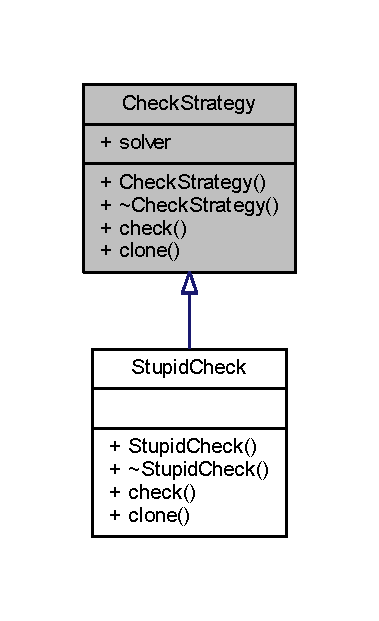
\includegraphics[width=182pt]{classCheckStrategy__inherit__graph}
\end{center}
\end{figure}


Check\+Strategy 的协作图\+:
\nopagebreak
\begin{figure}[H]
\begin{center}
\leavevmode
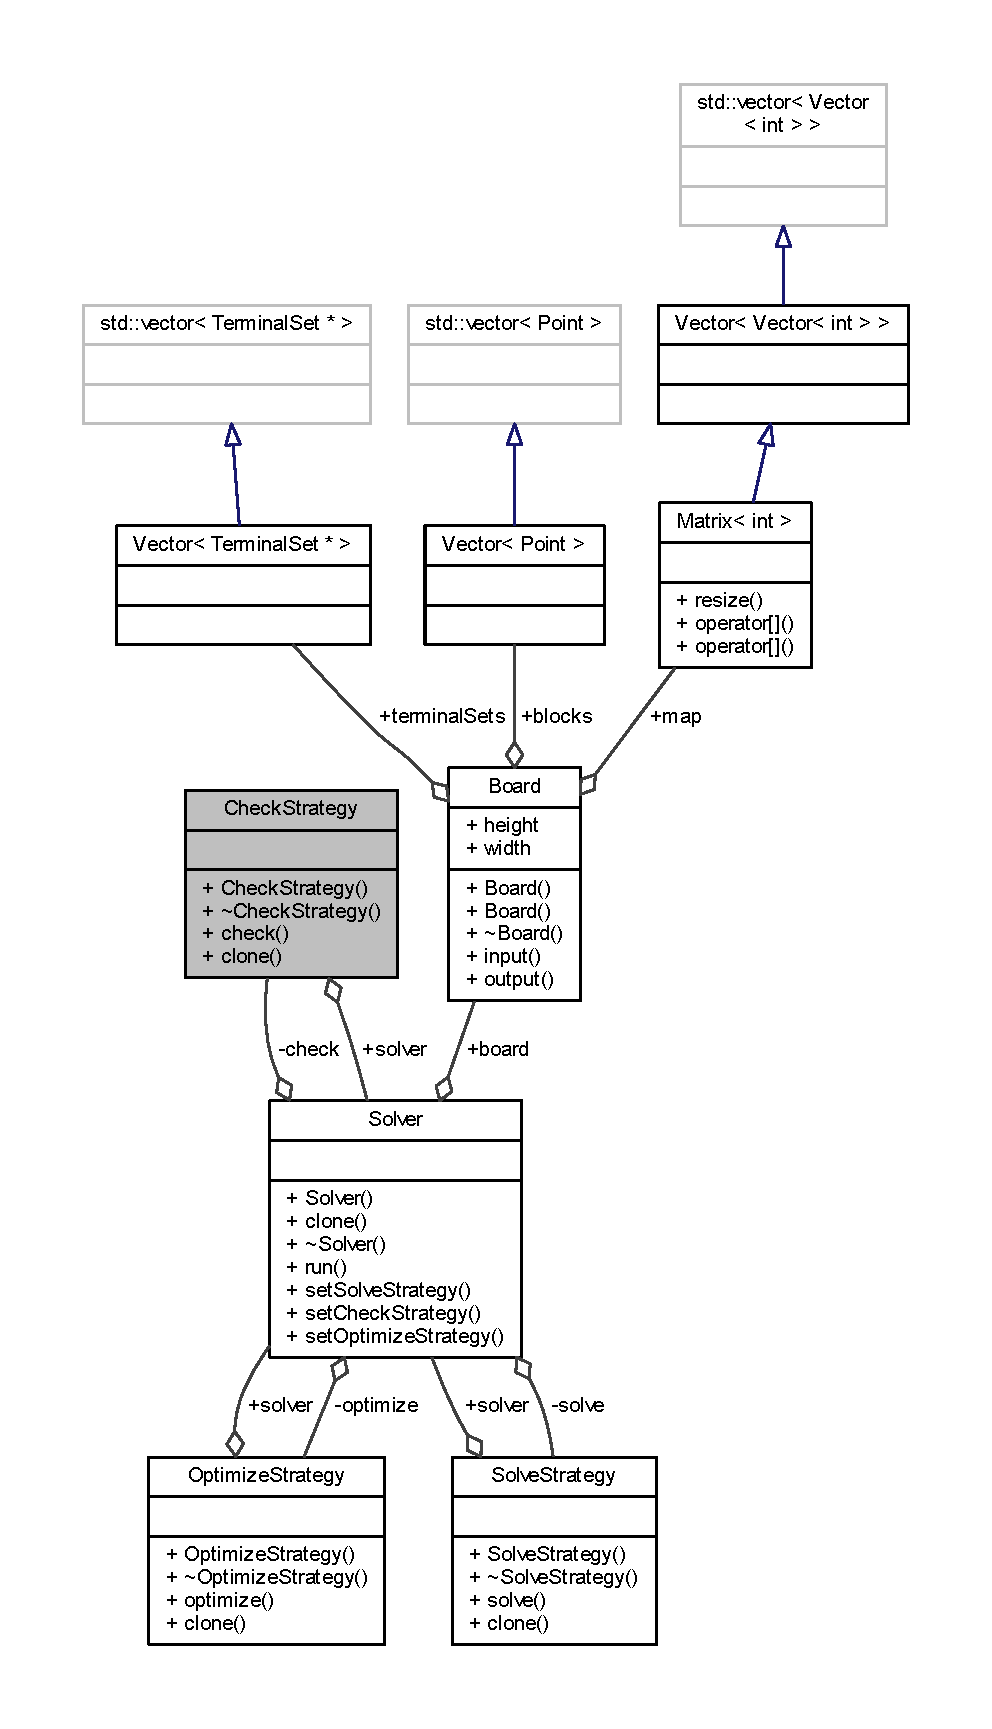
\includegraphics[height=550pt]{classCheckStrategy__coll__graph}
\end{center}
\end{figure}
\subsection*{Public 成员函数}
\begin{DoxyCompactItemize}
\item 
\hyperlink{classCheckStrategy_afdfa5dca2aecaccd079a765a1fb52690}{Check\+Strategy} (\hyperlink{classSolver}{Solver} $\ast$solver\+\_\+)
\item 
virtual \hyperlink{classCheckStrategy_a15162688463374268c2a008ba70b7327}{$\sim$\+Check\+Strategy} ()
\item 
virtual bool \hyperlink{classCheckStrategy_a4ea49fe480604a34b1a4604f61e34b11}{check} (const \hyperlink{classSolution}{Solution} \&\hyperlink{classes_8txt_aa43d5190bbc491d9c9134146e01a248e}{solution}) const  =0
\item 
virtual \hyperlink{classCheckStrategy}{Check\+Strategy} $\ast$ \hyperlink{classCheckStrategy_ae3d41d899831bf33314db410d7f2f947}{clone} () const  =0
\end{DoxyCompactItemize}
\subsection*{Public 属性}
\begin{DoxyCompactItemize}
\item 
\hyperlink{classSolver}{Solver} $\ast$ \hyperlink{classCheckStrategy_a2adc667c9f5fe299ef7fa0a01781448b}{solver}
\end{DoxyCompactItemize}


\subsection{详细描述}


在文件 Solve\+Strategy.\+h 第 23 行定义.



\subsection{构造及析构函数说明}
\index{Check\+Strategy@{Check\+Strategy}!Check\+Strategy@{Check\+Strategy}}
\index{Check\+Strategy@{Check\+Strategy}!Check\+Strategy@{Check\+Strategy}}
\subsubsection[{\texorpdfstring{Check\+Strategy(\+Solver $\ast$solver\+\_\+)}{CheckStrategy(Solver *solver_)}}]{\setlength{\rightskip}{0pt plus 5cm}Check\+Strategy\+::\+Check\+Strategy (
\begin{DoxyParamCaption}
\item[{{\bf Solver} $\ast$}]{solver\+\_\+}
\end{DoxyParamCaption}
)\hspace{0.3cm}{\ttfamily [inline]}}\hypertarget{classCheckStrategy_afdfa5dca2aecaccd079a765a1fb52690}{}\label{classCheckStrategy_afdfa5dca2aecaccd079a765a1fb52690}


在文件 Solve\+Strategy.\+h 第 28 行定义.


\begin{DoxyCode}
29     \{
30         \hyperlink{classCheckStrategy_a2adc667c9f5fe299ef7fa0a01781448b}{solver} = solver\_;
31     \}
\end{DoxyCode}
\index{Check\+Strategy@{Check\+Strategy}!````~Check\+Strategy@{$\sim$\+Check\+Strategy}}
\index{````~Check\+Strategy@{$\sim$\+Check\+Strategy}!Check\+Strategy@{Check\+Strategy}}
\subsubsection[{\texorpdfstring{$\sim$\+Check\+Strategy()}{~CheckStrategy()}}]{\setlength{\rightskip}{0pt plus 5cm}virtual Check\+Strategy\+::$\sim$\+Check\+Strategy (
\begin{DoxyParamCaption}
{}
\end{DoxyParamCaption}
)\hspace{0.3cm}{\ttfamily [inline]}, {\ttfamily [virtual]}}\hypertarget{classCheckStrategy_a15162688463374268c2a008ba70b7327}{}\label{classCheckStrategy_a15162688463374268c2a008ba70b7327}


在文件 Solve\+Strategy.\+h 第 32 行定义.



参考 Solve\+Strategy\+::clone() , 以及 solution.


\begin{DoxyCode}
32 \{\}
\end{DoxyCode}


函数调用图\+:
\nopagebreak
\begin{figure}[H]
\begin{center}
\leavevmode
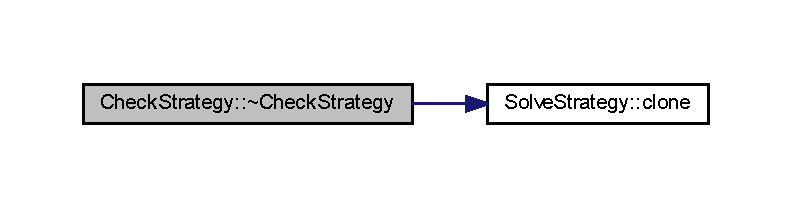
\includegraphics[width=350pt]{classCheckStrategy_a15162688463374268c2a008ba70b7327_cgraph}
\end{center}
\end{figure}




\subsection{成员函数说明}
\index{Check\+Strategy@{Check\+Strategy}!check@{check}}
\index{check@{check}!Check\+Strategy@{Check\+Strategy}}
\subsubsection[{\texorpdfstring{check(const Solution \&solution) const  =0}{check(const Solution &solution) const  =0}}]{\setlength{\rightskip}{0pt plus 5cm}virtual bool Check\+Strategy\+::check (
\begin{DoxyParamCaption}
\item[{const {\bf Solution} \&}]{solution}
\end{DoxyParamCaption}
) const\hspace{0.3cm}{\ttfamily [pure virtual]}}\hypertarget{classCheckStrategy_a4ea49fe480604a34b1a4604f61e34b11}{}\label{classCheckStrategy_a4ea49fe480604a34b1a4604f61e34b11}


在 \hyperlink{classStupidCheck_a6291b52893e1caf4dc84e195dc79e534}{Stupid\+Check} 内被实现.



参考自 Solver\+::run().



这是这个函数的调用关系图\+:
\nopagebreak
\begin{figure}[H]
\begin{center}
\leavevmode
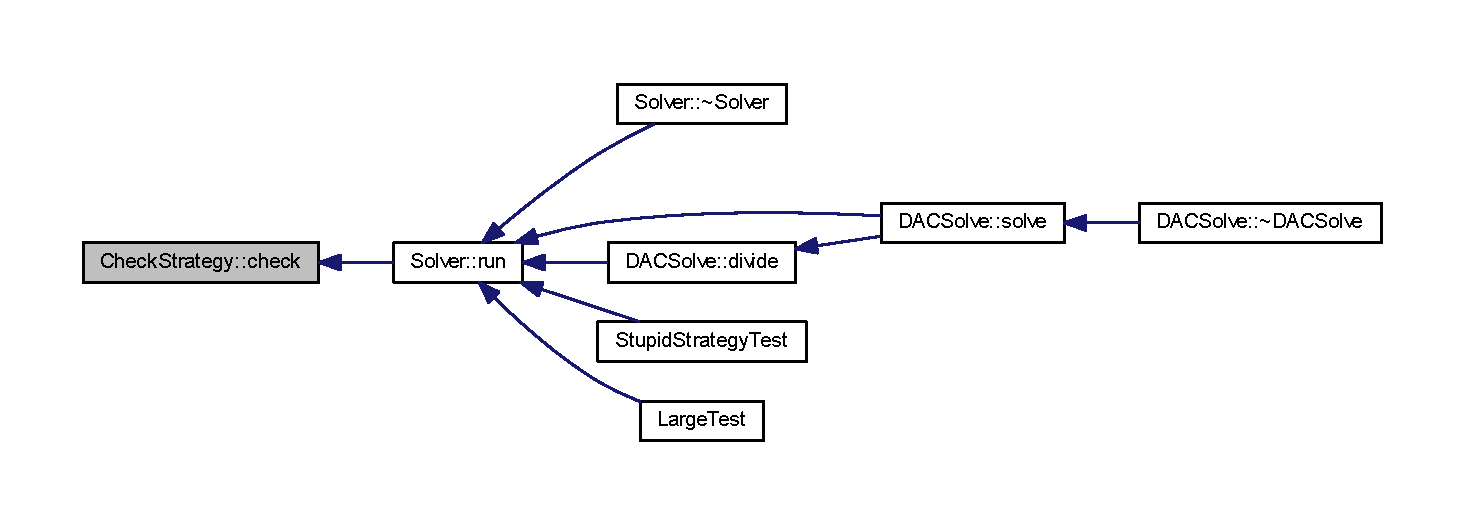
\includegraphics[width=350pt]{classCheckStrategy_a4ea49fe480604a34b1a4604f61e34b11_icgraph}
\end{center}
\end{figure}


\index{Check\+Strategy@{Check\+Strategy}!clone@{clone}}
\index{clone@{clone}!Check\+Strategy@{Check\+Strategy}}
\subsubsection[{\texorpdfstring{clone() const  =0}{clone() const  =0}}]{\setlength{\rightskip}{0pt plus 5cm}virtual {\bf Check\+Strategy}$\ast$ Check\+Strategy\+::clone (
\begin{DoxyParamCaption}
{}
\end{DoxyParamCaption}
) const\hspace{0.3cm}{\ttfamily [pure virtual]}}\hypertarget{classCheckStrategy_ae3d41d899831bf33314db410d7f2f947}{}\label{classCheckStrategy_ae3d41d899831bf33314db410d7f2f947}


在 \hyperlink{classStupidCheck_a5c2425603803daf7d190771623c78bcd}{Stupid\+Check} 内被实现.



参考自 Solver\+::clone().



这是这个函数的调用关系图\+:
\nopagebreak
\begin{figure}[H]
\begin{center}
\leavevmode
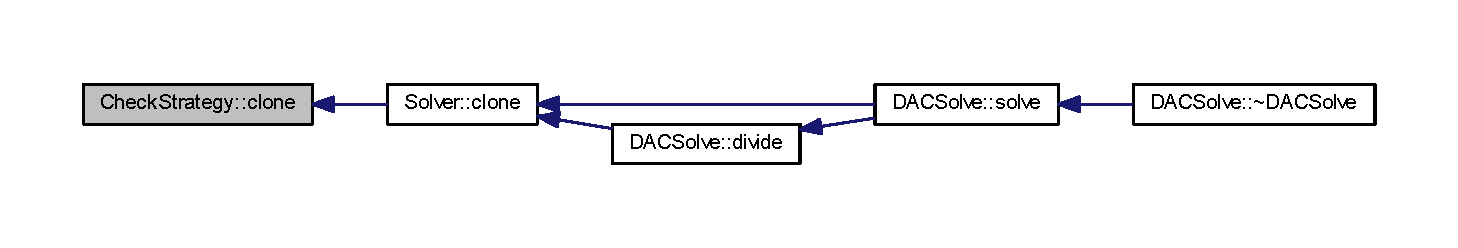
\includegraphics[width=350pt]{classCheckStrategy_ae3d41d899831bf33314db410d7f2f947_icgraph}
\end{center}
\end{figure}




\subsection{类成员变量说明}
\index{Check\+Strategy@{Check\+Strategy}!solver@{solver}}
\index{solver@{solver}!Check\+Strategy@{Check\+Strategy}}
\subsubsection[{\texorpdfstring{solver}{solver}}]{\setlength{\rightskip}{0pt plus 5cm}{\bf Solver}$\ast$ Check\+Strategy\+::solver}\hypertarget{classCheckStrategy_a2adc667c9f5fe299ef7fa0a01781448b}{}\label{classCheckStrategy_a2adc667c9f5fe299ef7fa0a01781448b}


在文件 Solve\+Strategy.\+h 第 27 行定义.



参考自 Solver\+::clone() , 以及 Solver\+::set\+Check\+Strategy().



该类的文档由以下文件生成\+:\begin{DoxyCompactItemize}
\item 
include/\hyperlink{SolveStrategy_8h}{Solve\+Strategy.\+h}\end{DoxyCompactItemize}

\hypertarget{classCleverOptimize}{}\section{Clever\+Optimize类 参考}
\label{classCleverOptimize}\index{Clever\+Optimize@{Clever\+Optimize}}


{\ttfamily \#include \char`\"{}Clever\+Optimize.\+h\char`\"{}}



类 Clever\+Optimize 继承关系图\+:
\nopagebreak
\begin{figure}[H]
\begin{center}
\leavevmode
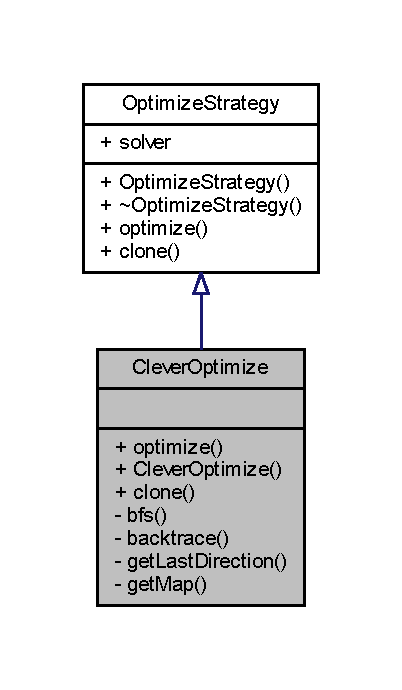
\includegraphics[width=193pt]{classCleverOptimize__inherit__graph}
\end{center}
\end{figure}


Clever\+Optimize 的协作图\+:
\nopagebreak
\begin{figure}[H]
\begin{center}
\leavevmode
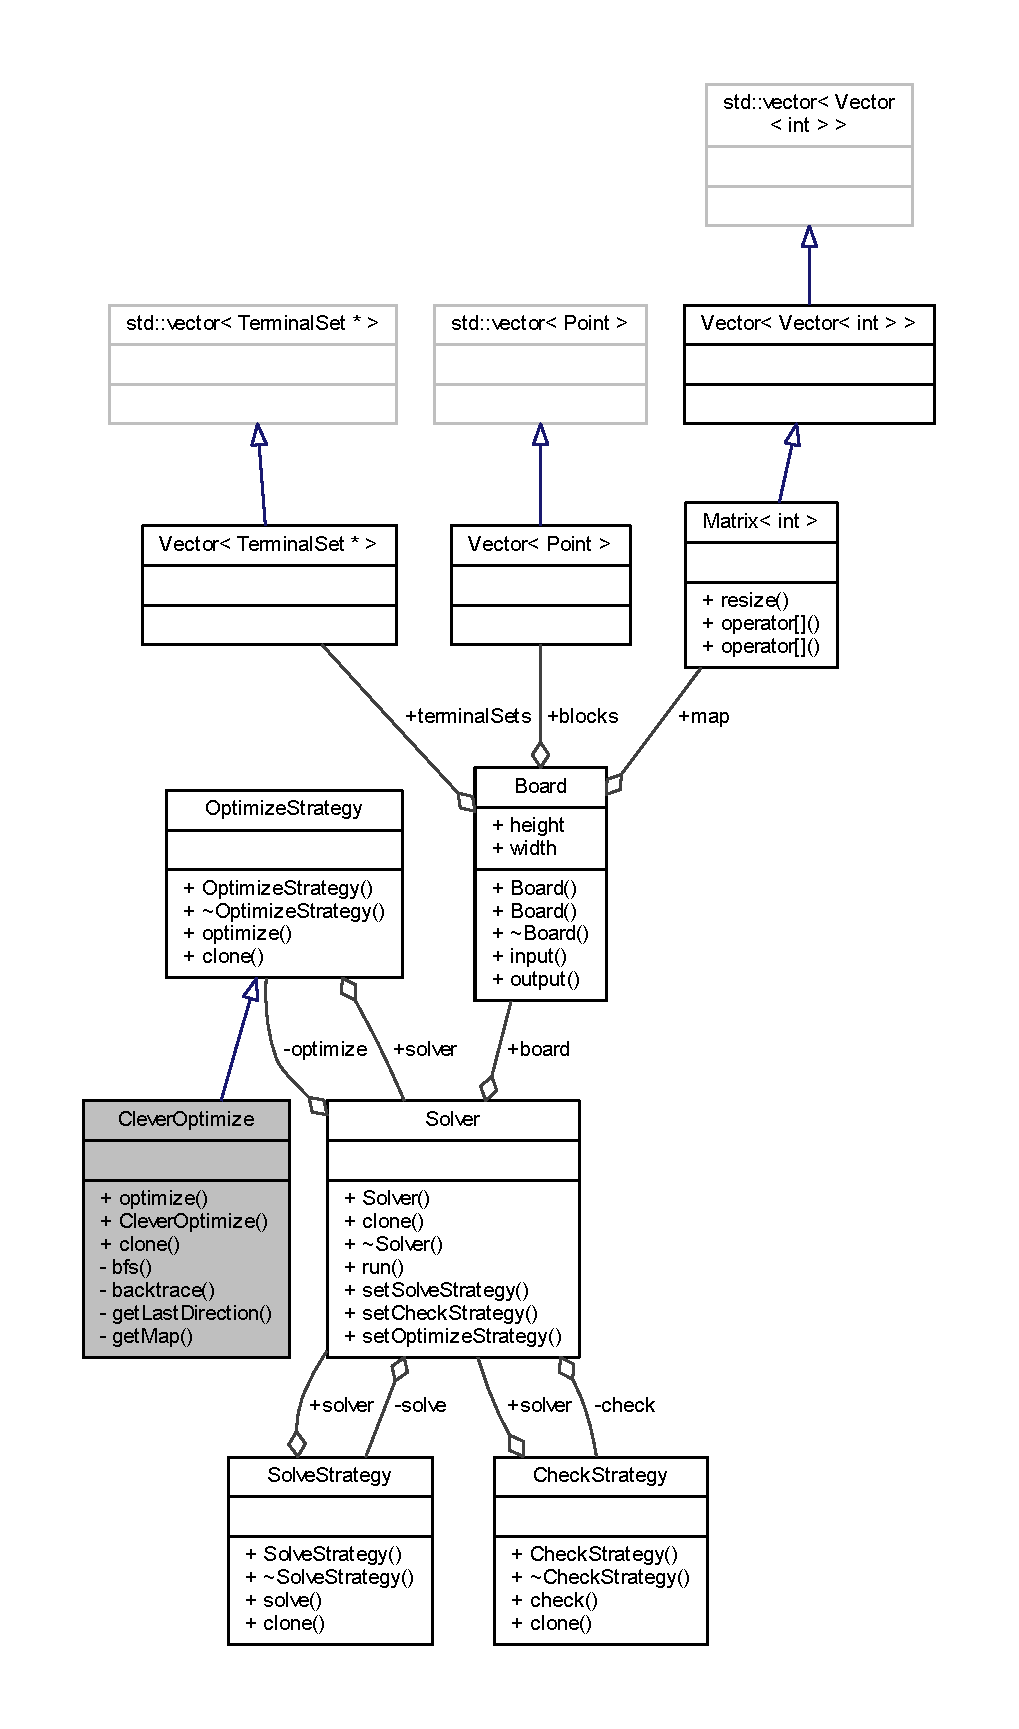
\includegraphics[height=550pt]{classCleverOptimize__coll__graph}
\end{center}
\end{figure}
\subsection*{Public 成员函数}
\begin{DoxyCompactItemize}
\item 
\hyperlink{classSolution}{Solution} \hyperlink{classCleverOptimize_ab3cc46af7f8e30d264c2f737870ab9e6}{optimize} (const \hyperlink{classSolution}{Solution} \&\hyperlink{classes_8txt_aa43d5190bbc491d9c9134146e01a248e}{solution}) const 
\item 
\hyperlink{classCleverOptimize_a84307b644b9fafa57d21042e02e9cdd3}{Clever\+Optimize} (\hyperlink{classSolver}{Solver} $\ast$solver\+\_\+)
\item 
virtual \hyperlink{classOptimizeStrategy}{Optimize\+Strategy} $\ast$ \hyperlink{classCleverOptimize_a64e5717a9e8090ccf6aecd185fbc9054}{clone} () const 
\end{DoxyCompactItemize}
\subsection*{Private 成员函数}
\begin{DoxyCompactItemize}
\item 
void \hyperlink{classCleverOptimize_a4b53de9bec3e3bbfd176ab68562a0df6}{bfs} (const \hyperlink{classPoint}{Point} \&start, \hyperlink{classBitMatrix}{Bit\+Matrix} \&\+\_\+map, \hyperlink{classBitMatrix}{Bit\+Matrix} \&\+\_\+compute\+Map, const \hyperlink{classSolution}{Solution} \&temp) const 
\item 
void \hyperlink{classCleverOptimize_ad4df8b31e69546d22b2066d33ef57c81}{backtrace} (const \hyperlink{classPoint}{Point} \&start, \hyperlink{classBitMatrix}{Bit\+Matrix} \&\hyperlink{classes_8txt_a0a12e395730487ab04f7f11cbc4d2132}{map}, \hyperlink{classMatrix}{Matrix}$<$ int $>$ \&visited, const \hyperlink{classPoint}{Point} \&end, int step) const 
\item 
int \hyperlink{classCleverOptimize_ac1cf58abb7c91bbabffde680d06226af}{get\+Last\+Direction} (const int k) const 
\item 
void \hyperlink{classCleverOptimize_a616cb7ecce678bca75c693230c7415ce}{get\+Map} (\hyperlink{classBitMatrix}{Bit\+Matrix} \&\+\_\+map, const \hyperlink{classPoint}{Point} \&start, \hyperlink{classBitMatrix}{Bit\+Matrix} \&\+\_\+origin\+Map) const 
\end{DoxyCompactItemize}
\subsection*{额外继承的成员函数}


\subsection{详细描述}


在文件 Clever\+Optimize.\+h 第 6 行定义.



\subsection{构造及析构函数说明}
\index{Clever\+Optimize@{Clever\+Optimize}!Clever\+Optimize@{Clever\+Optimize}}
\index{Clever\+Optimize@{Clever\+Optimize}!Clever\+Optimize@{Clever\+Optimize}}
\subsubsection[{\texorpdfstring{Clever\+Optimize(\+Solver $\ast$solver\+\_\+)}{CleverOptimize(Solver *solver_)}}]{\setlength{\rightskip}{0pt plus 5cm}Clever\+Optimize\+::\+Clever\+Optimize (
\begin{DoxyParamCaption}
\item[{{\bf Solver} $\ast$}]{solver\+\_\+}
\end{DoxyParamCaption}
)\hspace{0.3cm}{\ttfamily [inline]}}\hypertarget{classCleverOptimize_a84307b644b9fafa57d21042e02e9cdd3}{}\label{classCleverOptimize_a84307b644b9fafa57d21042e02e9cdd3}


在文件 Clever\+Optimize.\+h 第 15 行定义.



参考 clone().


\begin{DoxyCode}
15 : \hyperlink{classOptimizeStrategy_a4d2e0bc2a8590dd000428896bc26b7f0}{OptimizeStrategy}(solver\_)\{\}
\end{DoxyCode}


函数调用图\+:
\nopagebreak
\begin{figure}[H]
\begin{center}
\leavevmode
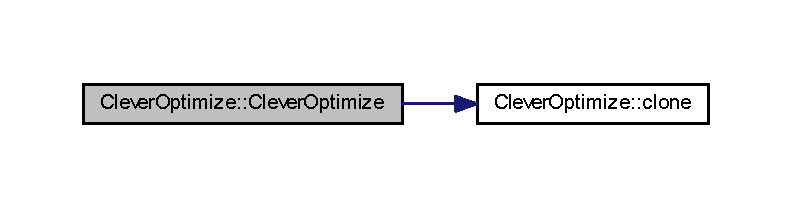
\includegraphics[width=350pt]{classCleverOptimize_a84307b644b9fafa57d21042e02e9cdd3_cgraph}
\end{center}
\end{figure}




\subsection{成员函数说明}
\index{Clever\+Optimize@{Clever\+Optimize}!backtrace@{backtrace}}
\index{backtrace@{backtrace}!Clever\+Optimize@{Clever\+Optimize}}
\subsubsection[{\texorpdfstring{backtrace(const Point \&start, Bit\+Matrix \&map, Matrix$<$ int $>$ \&visited, const Point \&end, int step) const }{backtrace(const Point &start, BitMatrix &map, Matrix< int > &visited, const Point &end, int step) const }}]{\setlength{\rightskip}{0pt plus 5cm}void Clever\+Optimize\+::backtrace (
\begin{DoxyParamCaption}
\item[{const {\bf Point} \&}]{start, }
\item[{{\bf Bit\+Matrix} \&}]{map, }
\item[{{\bf Matrix}$<$ int $>$ \&}]{visited, }
\item[{const {\bf Point} \&}]{end, }
\item[{int}]{step}
\end{DoxyParamCaption}
) const\hspace{0.3cm}{\ttfamily [private]}}\hypertarget{classCleverOptimize_ad4df8b31e69546d22b2066d33ef57c81}{}\label{classCleverOptimize_ad4df8b31e69546d22b2066d33ef57c81}


在文件 Clever\+Optimizie.\+cpp 第 204 行定义.



参考 Bit\+Matrix\+::height, Bit\+Matrix\+::set(), X, Point\+::x, Y , 以及 Point\+::y.


\begin{DoxyCode}
205 \{
206     \hyperlink{classPoint}{Point} currentPoint = end;
207     \textcolor{keywordflow}{while} (currentPoint != start)
208     \{
209         step = step - 1;
210         \textcolor{keywordflow}{for} (\textcolor{keywordtype}{int} i = 1;i <= 4;++i)
211         \{
212             \textcolor{keywordtype}{int} currentx = \hyperlink{CleverOptimizie_8cpp_a34adaf40bb2f109e151ba28ccc73c677}{X}[i] + currentPoint.\hyperlink{classPoint_a8c779e11e694b20e0946105a9f5de842}{x};
213             \textcolor{keywordtype}{int} currenty = \hyperlink{CleverOptimizie_8cpp_a86f15c23d2ab23bfebe784c368885663}{Y}[i] + currentPoint.\hyperlink{classPoint_a2e1b5fb2b2a83571f5c0bc0f66a73cf7}{y};
214             \textcolor{keywordflow}{if} (currenty >= 0 && currenty < map.width && currentx >= 0 && currentx < map.
      \hyperlink{classBitMatrix_a3b7a1be96313cacfd3b2a08661dd919c}{height})
215             \{
216                 \textcolor{keywordflow}{if} (visited[currentx][currenty] == step)
217                 \{
218                     currentPoint = \hyperlink{classPoint}{Point}(currentx,currenty);
219                     map.\hyperlink{classBitMatrix_ad26dd2e93e9d24d70834d6d79e29c81e}{set}(currentx,currenty);
220                     \textcolor{keywordflow}{break};
221                 \}
222             \}
223         \}
224     \}
225 \}
\end{DoxyCode}


函数调用图\+:
\nopagebreak
\begin{figure}[H]
\begin{center}
\leavevmode
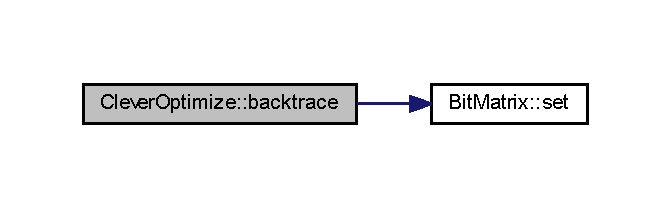
\includegraphics[width=322pt]{classCleverOptimize_ad4df8b31e69546d22b2066d33ef57c81_cgraph}
\end{center}
\end{figure}


\index{Clever\+Optimize@{Clever\+Optimize}!bfs@{bfs}}
\index{bfs@{bfs}!Clever\+Optimize@{Clever\+Optimize}}
\subsubsection[{\texorpdfstring{bfs(const Point \&start, Bit\+Matrix \&\+\_\+map, Bit\+Matrix \&\+\_\+compute\+Map, const Solution \&temp) const }{bfs(const Point &start, BitMatrix &_map, BitMatrix &_computeMap, const Solution &temp) const }}]{\setlength{\rightskip}{0pt plus 5cm}void Clever\+Optimize\+::bfs (
\begin{DoxyParamCaption}
\item[{const {\bf Point} \&}]{start, }
\item[{{\bf Bit\+Matrix} \&}]{\+\_\+map, }
\item[{{\bf Bit\+Matrix} \&}]{\+\_\+compute\+Map, }
\item[{const {\bf Solution} \&}]{temp}
\end{DoxyParamCaption}
) const\hspace{0.3cm}{\ttfamily [private]}}\hypertarget{classCleverOptimize_a4b53de9bec3e3bbfd176ab68562a0df6}{}\label{classCleverOptimize_a4b53de9bec3e3bbfd176ab68562a0df6}


在文件 Clever\+Optimizie.\+cpp 第 156 行定义.



参考 Solution\+::board, Bit\+Matrix\+::get(), Bit\+Matrix\+::height, Board\+::map, Solution\+::map, Matrix$<$ T $>$\+::resize(), Bit\+Matrix\+::width, X, Point\+::x, Y , 以及 Point\+::y.


\begin{DoxyCode}
157 \{
158     \hyperlink{classMatrix}{Matrix<int>} visited;
159     list<Point> waitingPoints;
160     waitingPoints.push\_back(start);
161     visited.\hyperlink{classMatrix_a15ce96c8af4c7a982c2c10b96f29cea1}{resize}(\_map.\hyperlink{classBitMatrix_a3b7a1be96313cacfd3b2a08661dd919c}{height},\_map.\hyperlink{classBitMatrix_ac271de23ac5446a0a75ee457a385d882}{width});
162     visited[start.\hyperlink{classPoint_a8c779e11e694b20e0946105a9f5de842}{x}][start.\hyperlink{classPoint_a2e1b5fb2b2a83571f5c0bc0f66a73cf7}{y}] = 1;
163     \textcolor{keywordtype}{bool} find = \textcolor{keyword}{false};
164     \textcolor{keywordtype}{int} step = 1;
165     \textcolor{keywordflow}{while} (!waitingPoints.empty() && !find)
166     \{
167         \hyperlink{classPoint}{Point} currentPoint = waitingPoints.front();
168         waitingPoints.pop\_front();
169         step = visited[currentPoint.\hyperlink{classPoint_a8c779e11e694b20e0946105a9f5de842}{x}][currentPoint.\hyperlink{classPoint_a2e1b5fb2b2a83571f5c0bc0f66a73cf7}{y}] + 1;
170         \textcolor{keywordflow}{for} (\textcolor{keywordtype}{int} i = 1;i <= 4;++i)
171         \{
172             \textcolor{keywordtype}{int} currentx = \hyperlink{CleverOptimizie_8cpp_a34adaf40bb2f109e151ba28ccc73c677}{X}[i] + currentPoint.\hyperlink{classPoint_a8c779e11e694b20e0946105a9f5de842}{x};
173             \textcolor{keywordtype}{int} currenty = \hyperlink{CleverOptimizie_8cpp_a86f15c23d2ab23bfebe784c368885663}{Y}[i] + currentPoint.\hyperlink{classPoint_a2e1b5fb2b2a83571f5c0bc0f66a73cf7}{y};
174                 \textcolor{keywordflow}{if} (currenty >= 0 && currenty < 
175                     \_map.\hyperlink{classBitMatrix_ac271de23ac5446a0a75ee457a385d882}{width} && currentx >= 0 && currentx < \_map.\hyperlink{classBitMatrix_a3b7a1be96313cacfd3b2a08661dd919c}{height})
176                 \textcolor{keywordflow}{if} (!visited[currentx][currenty] && !(temp.\hyperlink{classSolution_ac4f88cd3aa0713e8900f33eb9f1f15bf}{board}->\hyperlink{classBoard_a191ff45df9151b8fee0c32877f582165}{map}[currentx][currenty] == -1) 
177                     && ((\_map.\hyperlink{classBitMatrix_ad19d1045b54ccc8a99d70d38305b4ca6}{get}(currentx,currenty)^(temp.\hyperlink{classSolution_ae89ccd74484f2c87afa05b16f8ee5bf6}{map}[currentx][currenty] > 0)) == 0))
178                 \{
179                     \textcolor{comment}{// cout<<currentx<<"now"<<currenty<<endl;}
180                     visited[currentx][currenty] = step;
181                     waitingPoints.push\_back(\hyperlink{classPoint}{Point}(currentx,currenty));
182                     \textcolor{keywordflow}{if} (\_computedMap.get(currentx,currenty) == 1)
183                     \{
184                         \textcolor{comment}{// cout<<"true"<<currentx<<' '<<currenty<<endl;}
185                         \textcolor{comment}{// cout<<"currentPoint"<<currentPoint.x<<' '<<currentPoint.y<<endl;}
186                         find  = \textcolor{keyword}{true};
187                         \textcolor{comment}{// cout<<"bfs completed"<<endl;}
188                         \textcolor{keywordflow}{for} (\textcolor{keywordtype}{int} i = 0;i < \_map.\hyperlink{classBitMatrix_ac271de23ac5446a0a75ee457a385d882}{width}; ++i)
189                         \{
190                             \textcolor{keywordflow}{for} (\textcolor{keywordtype}{int} j = 0;j < \_map.\hyperlink{classBitMatrix_a3b7a1be96313cacfd3b2a08661dd919c}{height}; ++j)
191                                 cout<<visited[i][j]<<\textcolor{charliteral}{' '};
192                             \textcolor{comment}{// cout<<endl;}
193                         \}
194                         \hyperlink{classCleverOptimize_ad4df8b31e69546d22b2066d33ef57c81}{backtrace}(start,\_map,visited,\hyperlink{classPoint}{Point}(currentx,currenty),step);
195                         \textcolor{comment}{// cout<<\_map<<endl;}
196                         find = \textcolor{keyword}{true};
197                         \textcolor{keywordflow}{break};
198                     \}
199                 \}
200         \}
201     \}
202 \}
\end{DoxyCode}


函数调用图\+:
\nopagebreak
\begin{figure}[H]
\begin{center}
\leavevmode
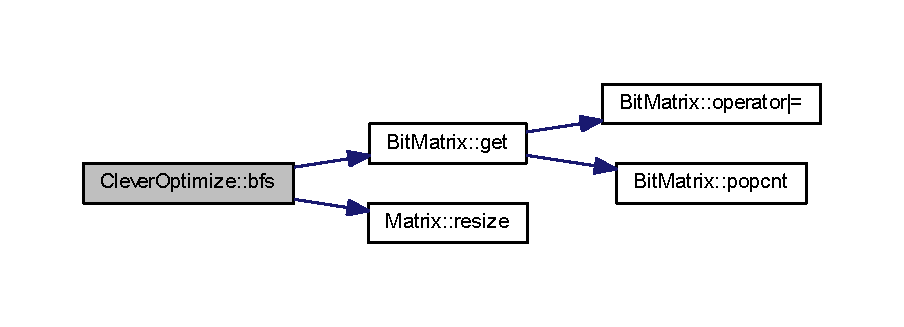
\includegraphics[width=350pt]{classCleverOptimize_a4b53de9bec3e3bbfd176ab68562a0df6_cgraph}
\end{center}
\end{figure}


\index{Clever\+Optimize@{Clever\+Optimize}!clone@{clone}}
\index{clone@{clone}!Clever\+Optimize@{Clever\+Optimize}}
\subsubsection[{\texorpdfstring{clone() const }{clone() const }}]{\setlength{\rightskip}{0pt plus 5cm}{\bf Optimize\+Strategy} $\ast$ Clever\+Optimize\+::clone (
\begin{DoxyParamCaption}
{}
\end{DoxyParamCaption}
) const\hspace{0.3cm}{\ttfamily [virtual]}}\hypertarget{classCleverOptimize_a64e5717a9e8090ccf6aecd185fbc9054}{}\label{classCleverOptimize_a64e5717a9e8090ccf6aecd185fbc9054}


实现了 \hyperlink{classOptimizeStrategy_a3cf14f98ef8800d2e6c67ddd610edcbd}{Optimize\+Strategy}.



在文件 Clever\+Optimizie.\+cpp 第 227 行定义.



参考自 Clever\+Optimize().


\begin{DoxyCode}
228 \{
229     \textcolor{keywordflow}{return} \textcolor{keyword}{new} \hyperlink{classCleverOptimize_a84307b644b9fafa57d21042e02e9cdd3}{CleverOptimize}(*\textcolor{keyword}{this});
230 \}
\end{DoxyCode}


这是这个函数的调用关系图\+:
\nopagebreak
\begin{figure}[H]
\begin{center}
\leavevmode
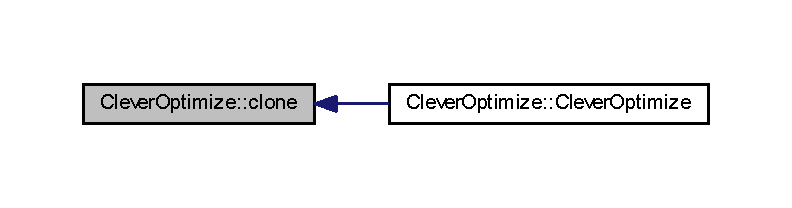
\includegraphics[width=350pt]{classCleverOptimize_a64e5717a9e8090ccf6aecd185fbc9054_icgraph}
\end{center}
\end{figure}


\index{Clever\+Optimize@{Clever\+Optimize}!get\+Last\+Direction@{get\+Last\+Direction}}
\index{get\+Last\+Direction@{get\+Last\+Direction}!Clever\+Optimize@{Clever\+Optimize}}
\subsubsection[{\texorpdfstring{get\+Last\+Direction(const int k) const }{getLastDirection(const int k) const }}]{\setlength{\rightskip}{0pt plus 5cm}int Clever\+Optimize\+::get\+Last\+Direction (
\begin{DoxyParamCaption}
\item[{const int}]{k}
\end{DoxyParamCaption}
) const\hspace{0.3cm}{\ttfamily [private]}}\hypertarget{classCleverOptimize_ac1cf58abb7c91bbabffde680d06226af}{}\label{classCleverOptimize_ac1cf58abb7c91bbabffde680d06226af}


在文件 Clever\+Optimizie.\+cpp 第 116 行定义.


\begin{DoxyCode}
117 \{
118     \textcolor{keywordflow}{if} (k == 1) \textcolor{keywordflow}{return} 3;
119     \textcolor{keywordflow}{if} (k == 2) \textcolor{keywordflow}{return} 4;
120     \textcolor{keywordflow}{if} (k == 3) \textcolor{keywordflow}{return} 1;
121     \textcolor{keywordflow}{if} (k == 4) \textcolor{keywordflow}{return} 2;
122     \textcolor{keywordflow}{return} 0;
123 \}
\end{DoxyCode}
\index{Clever\+Optimize@{Clever\+Optimize}!get\+Map@{get\+Map}}
\index{get\+Map@{get\+Map}!Clever\+Optimize@{Clever\+Optimize}}
\subsubsection[{\texorpdfstring{get\+Map(\+Bit\+Matrix \&\+\_\+map, const Point \&start, Bit\+Matrix \&\+\_\+origin\+Map) const }{getMap(BitMatrix &_map, const Point &start, BitMatrix &_originMap) const }}]{\setlength{\rightskip}{0pt plus 5cm}void Clever\+Optimize\+::get\+Map (
\begin{DoxyParamCaption}
\item[{{\bf Bit\+Matrix} \&}]{\+\_\+map, }
\item[{const {\bf Point} \&}]{start, }
\item[{{\bf Bit\+Matrix} \&}]{\+\_\+origin\+Map}
\end{DoxyParamCaption}
) const\hspace{0.3cm}{\ttfamily [private]}}\hypertarget{classCleverOptimize_a616cb7ecce678bca75c693230c7415ce}{}\label{classCleverOptimize_a616cb7ecce678bca75c693230c7415ce}


在文件 Clever\+Optimizie.\+cpp 第 125 行定义.



参考 Bit\+Matrix\+::get(), Bit\+Matrix\+::height, Matrix$<$ T $>$\+::resize(), Bit\+Matrix\+::set(), Bit\+Matrix\+::width, X, Point\+::x, Y , 以及 Point\+::y.


\begin{DoxyCode}
126 \{
127     \hyperlink{classMatrix}{Matrix<int>} visited;
128     visited.\hyperlink{classMatrix_a15ce96c8af4c7a982c2c10b96f29cea1}{resize}(\_map.\hyperlink{classBitMatrix_a3b7a1be96313cacfd3b2a08661dd919c}{height},\_map.\hyperlink{classBitMatrix_ac271de23ac5446a0a75ee457a385d882}{width});
129     list<Point> waitingPoints;
130     waitingPoints.push\_back(start);
131     visited[start.\hyperlink{classPoint_a8c779e11e694b20e0946105a9f5de842}{x}][start.\hyperlink{classPoint_a2e1b5fb2b2a83571f5c0bc0f66a73cf7}{y}] = 1;
132     \textcolor{comment}{// cout<<start.x<<' '<<start.y<<endl;}
133     \_map.\hyperlink{classBitMatrix_ad26dd2e93e9d24d70834d6d79e29c81e}{set}(start.\hyperlink{classPoint_a8c779e11e694b20e0946105a9f5de842}{x},start.\hyperlink{classPoint_a2e1b5fb2b2a83571f5c0bc0f66a73cf7}{y});
134     \textcolor{comment}{// cout<<"start"<<\_map<<endl;}
135     \textcolor{keywordflow}{while} (!waitingPoints.empty())
136     \{
137         \hyperlink{classPoint}{Point} currentPoint = waitingPoints.front();
138         waitingPoints.pop\_front();
139         \textcolor{keywordflow}{for} (\textcolor{keywordtype}{int} i = 1;i <= 4;++i)
140         \{
141             \textcolor{keywordtype}{int} currentx = \hyperlink{CleverOptimizie_8cpp_a34adaf40bb2f109e151ba28ccc73c677}{X}[i] + currentPoint.\hyperlink{classPoint_a8c779e11e694b20e0946105a9f5de842}{x};
142             \textcolor{keywordtype}{int} currenty = \hyperlink{CleverOptimizie_8cpp_a86f15c23d2ab23bfebe784c368885663}{Y}[i] + currentPoint.\hyperlink{classPoint_a2e1b5fb2b2a83571f5c0bc0f66a73cf7}{y};
143             \textcolor{keywordflow}{if} (currenty >= 0 && currenty < \_map.width && currentx >= 0 && currentx < \_map.
      \hyperlink{classBitMatrix_a3b7a1be96313cacfd3b2a08661dd919c}{height})
144             \{
145                 \textcolor{keywordflow}{if} (!visited[currentx][currenty] && \_originMap.\hyperlink{classBitMatrix_ad19d1045b54ccc8a99d70d38305b4ca6}{get}(currentx,currenty) == 1)
146                 \{
147                     waitingPoints.push\_back(\hyperlink{classPoint}{Point}(currentx,currenty));
148                     \_map.\hyperlink{classBitMatrix_ad26dd2e93e9d24d70834d6d79e29c81e}{set}(currentx,currenty);
149                     visited[currentx][currenty] = 1;
150                 \}
151             \}
152         \}
153     \}
154 \}
\end{DoxyCode}


函数调用图\+:
\nopagebreak
\begin{figure}[H]
\begin{center}
\leavevmode
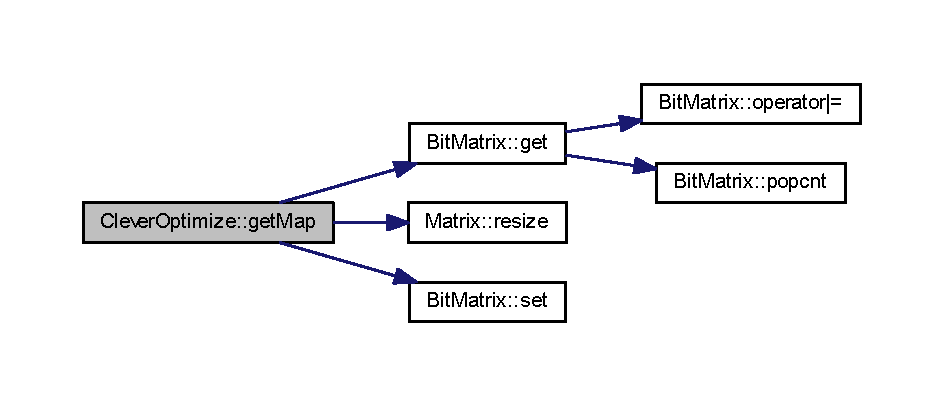
\includegraphics[width=350pt]{classCleverOptimize_a616cb7ecce678bca75c693230c7415ce_cgraph}
\end{center}
\end{figure}


\index{Clever\+Optimize@{Clever\+Optimize}!optimize@{optimize}}
\index{optimize@{optimize}!Clever\+Optimize@{Clever\+Optimize}}
\subsubsection[{\texorpdfstring{optimize(const Solution \&solution) const }{optimize(const Solution &solution) const }}]{\setlength{\rightskip}{0pt plus 5cm}{\bf Solution} Clever\+Optimize\+::optimize (
\begin{DoxyParamCaption}
\item[{const {\bf Solution} \&}]{solution}
\end{DoxyParamCaption}
) const\hspace{0.3cm}{\ttfamily [virtual]}}\hypertarget{classCleverOptimize_ab3cc46af7f8e30d264c2f737870ab9e6}{}\label{classCleverOptimize_ab3cc46af7f8e30d264c2f737870ab9e6}


实现了 \hyperlink{classOptimizeStrategy_a2ac1b1c33fa54a59e6f3a9daffcbf4eb}{Optimize\+Strategy}.



在文件 Clever\+Optimizie.\+cpp 第 10 行定义.



参考 Solution\+::board, Solution\+::compute\+Map(), Board\+::map, Solution\+::trees, X, Point\+::x, Y , 以及 Point\+::y.



参考自 T\+E\+S\+T().


\begin{DoxyCode}
11 \{
12     \hyperlink{classSolution}{Solution} temp(solution);
13     \textcolor{keywordflow}{for} (\textcolor{keywordtype}{unsigned} i = 1;i < temp.trees.size();++i)
14     \{
15         \textcolor{keywordflow}{for} (\textcolor{keywordtype}{unsigned} j = 0;j < temp.trees[i]->terminalSet->points.size();++j)
16         \{
17             \textcolor{keywordtype}{int} degree = 0,lastDirection = 0;
18             \textcolor{keywordtype}{bool} noNeedToChange = \textcolor{keyword}{true};
19             \hyperlink{classPoint}{Point} currentPoint(temp.trees[i]->terminalSet->points[j].x,temp.trees[i]->terminalSet->
      points[j].y);
20             \textcolor{keywordflow}{for} (\textcolor{keywordtype}{int} k = 1;k <= 4; ++k)
21             \{
22                 \textcolor{comment}{// cout<<currentPoint.x<<currentPoint.y<<endl;  }
23                 \textcolor{keywordtype}{int} currentx = \hyperlink{CleverOptimizie_8cpp_a34adaf40bb2f109e151ba28ccc73c677}{X}[k] + currentPoint.x;
24                 \textcolor{keywordtype}{int} currenty = \hyperlink{CleverOptimizie_8cpp_a86f15c23d2ab23bfebe784c368885663}{Y}[k] + currentPoint.y;
25                 \textcolor{comment}{// cout<<"cur"<<currentx<<currenty<<endl;}
26                 \textcolor{keywordflow}{if} (currenty >= 0 && currenty < temp.trees[i]->map.width && currentx >= 0 && currentx < 
      temp.trees[i]->map.height)
27                 \{
28                     \textcolor{keywordflow}{if} (temp.trees[i]->map.get(currentx,currenty) == 1) 
29                     \{
30                         vector<Point>  resetedPoints;
31                         lastDirection = k;
32                         \textcolor{comment}{// cout<<k<<' '<<currentPoint.x<<' '<<currentPoint.y<<endl;}
33                         \hyperlink{classPoint}{Point} tempPoint(currentx,currenty);
34                         \textcolor{keywordflow}{while} (degree <= 2)
35                         \{
36                             \textcolor{keywordflow}{for} (\textcolor{keywordtype}{int} u = 1;u <= 4; ++u)
37                             \{
38                                 currentx = \hyperlink{CleverOptimizie_8cpp_a34adaf40bb2f109e151ba28ccc73c677}{X}[u] + tempPoint.x;
39                                 currenty = \hyperlink{CleverOptimizie_8cpp_a86f15c23d2ab23bfebe784c368885663}{Y}[u] + tempPoint.y;
40                                 \textcolor{keywordflow}{if} (currenty >= 0 && currenty < temp.trees[i]->map.width && currentx >= 0 
      && currentx < temp.trees[i]->map.height)
41                                 \{
42                                     \textcolor{keywordflow}{if} (temp.trees[i]->map.get(currentx,currenty) == 1 
43                                     && !(temp.board->map[currentx][currenty] > 0)) 
44                                     \{
45                                         \textcolor{keywordflow}{if} (u != \hyperlink{classCleverOptimize_ac1cf58abb7c91bbabffde680d06226af}{getLastDirection}(lastDirection))
46                                         \{
47                                             degree++;
48                                             \textcolor{comment}{// cout<<tempPoint.x<<' '<<tempPoint.y<<' '<<currentx<<'
       '<<currenty<<endl;}
49                                         \}
50                                     \}
51                                 \}
52                             \}
53                             \textcolor{comment}{// cout<<"degree : "<<degree<<endl;}
54                             \textcolor{keywordflow}{if} (degree >= 2)
55                             \{
56                                 noNeedToChange = \textcolor{keyword}{false};
57                                 \textcolor{keywordflow}{break};
58                             \}
59                             \textcolor{keywordflow}{else} \textcolor{keywordflow}{if} (degree == 0) \textcolor{keywordflow}{break};
60                             \textcolor{keywordflow}{else}
61                             \{
62                                 \textcolor{keywordflow}{if} (temp.board->map[tempPoint.x][tempPoint.y] != 0) \textcolor{keywordflow}{break};
63                                 temp.trees[i]->map.reset(tempPoint.x,tempPoint.y);
64                                 temp.computeMap();
65                                 resetedPoints.push\_back(tempPoint);
66                                 degree = 0;
67                                 \textcolor{keywordflow}{for} (\textcolor{keywordtype}{int} u = 1;u <= 4; ++u)
68                                 \{
69                                     currentx = \hyperlink{CleverOptimizie_8cpp_a34adaf40bb2f109e151ba28ccc73c677}{X}[u] + tempPoint.x;
70                                     currenty = \hyperlink{CleverOptimizie_8cpp_a86f15c23d2ab23bfebe784c368885663}{Y}[u] + tempPoint.y;
71                                     \textcolor{keywordflow}{if} (currenty >= 0 && currenty < temp.trees[i]->map.width && currentx >=
       0 && currentx < temp.trees[i]->map.height)
72                                     \{
73                                         \textcolor{keywordflow}{if} (temp.trees[i]->map.get(currentx,currenty) == 1) 
74                                         \{
75                                             \textcolor{comment}{// cout<<u<<' '<<lastDirection<<endl;}
76                                             \textcolor{keywordflow}{if} (u != \hyperlink{classCleverOptimize_ac1cf58abb7c91bbabffde680d06226af}{getLastDirection}(lastDirection))
77                                             \{
78                                                 lastDirection = u;
79                                                 \textcolor{keywordflow}{break};
80                                             \}
81                                         \}
82                                     \}
83                                 \}
84                                 tempPoint.x += \hyperlink{CleverOptimizie_8cpp_a34adaf40bb2f109e151ba28ccc73c677}{X}[lastDirection];
85                                 tempPoint.y += \hyperlink{CleverOptimizie_8cpp_a86f15c23d2ab23bfebe784c368885663}{Y}[lastDirection];
86                             \}
87                             \textcolor{comment}{// cout<<i<<' '<<j<<' '<<degree<<endl;}
88                         \}
89                         \textcolor{keywordflow}{if} (!noNeedToChange)
90                         \{
91                             \textcolor{comment}{// cout<<temp<<endl;}
92                             \hyperlink{classBitMatrix}{BitMatrix} \_map(temp.trees[i]->map.height,temp.trees[i]->map.width);
93                             \hyperlink{classCleverOptimize_a616cb7ecce678bca75c693230c7415ce}{getMap}(\_map,tempPoint,temp.trees[i]->map);
94                             \textcolor{comment}{// cout<<\_map;}
95                             \hyperlink{classCleverOptimize_a4b53de9bec3e3bbfd176ab68562a0df6}{bfs}(temp.trees[i]->terminalSet->points[j],temp.trees[i]->map,\_map,temp);
96                             temp.computeMap();
97                             \textcolor{comment}{// cout<<temp.trees[i]->map<<endl;}
98                             \textcolor{comment}{// cout<<temp<<endl;}
99                         \}
100                         \textcolor{keywordflow}{else}
101                         \{
102                             \textcolor{comment}{// cout<<"reseting..."<<endl;}
103                             \textcolor{keywordflow}{for} (\textcolor{keywordtype}{unsigned} \textcolor{keywordtype}{int} u = 0;u < resetedPoints.size();++u)
104                                 temp.trees[i]->map.set(resetedPoints[u].x,resetedPoints[u].y);
105                             temp.computeMap();
106                         \}
107                         \textcolor{comment}{// cout<<temp<<endl;}
108                     \}
109                 \}
110             \}   
111         \}
112     \}
113     \textcolor{keywordflow}{return} temp;
114 \}
\end{DoxyCode}


函数调用图\+:
\nopagebreak
\begin{figure}[H]
\begin{center}
\leavevmode
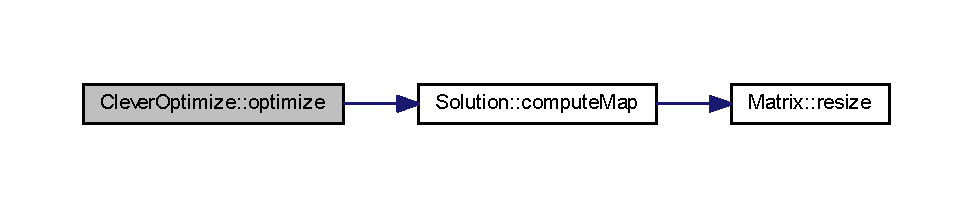
\includegraphics[width=350pt]{classCleverOptimize_ab3cc46af7f8e30d264c2f737870ab9e6_cgraph}
\end{center}
\end{figure}




这是这个函数的调用关系图\+:
\nopagebreak
\begin{figure}[H]
\begin{center}
\leavevmode
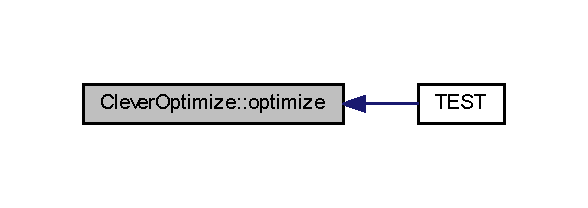
\includegraphics[width=282pt]{classCleverOptimize_ab3cc46af7f8e30d264c2f737870ab9e6_icgraph}
\end{center}
\end{figure}




该类的文档由以下文件生成\+:\begin{DoxyCompactItemize}
\item 
include/\hyperlink{CleverOptimize_8h}{Clever\+Optimize.\+h}\item 
src/\hyperlink{CleverOptimizie_8cpp}{Clever\+Optimizie.\+cpp}\end{DoxyCompactItemize}

\hypertarget{classColumnGenSolve}{}\section{Column\+Gen\+Solve类 参考}
\label{classColumnGenSolve}\index{Column\+Gen\+Solve@{Column\+Gen\+Solve}}


{\ttfamily \#include \char`\"{}Column\+Gen\+Solve.\+h\char`\"{}}



类 Column\+Gen\+Solve 继承关系图\+:
\nopagebreak
\begin{figure}[H]
\begin{center}
\leavevmode
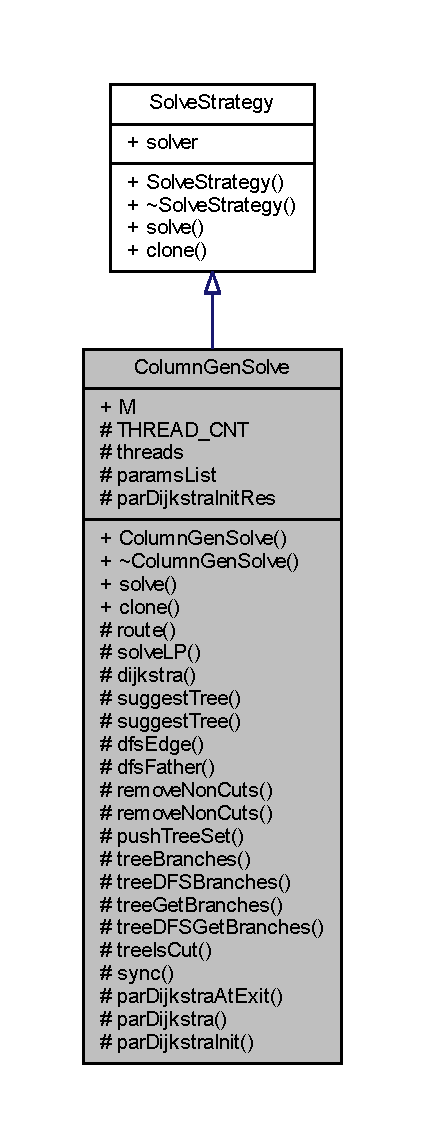
\includegraphics[height=550pt]{classColumnGenSolve__inherit__graph}
\end{center}
\end{figure}


Column\+Gen\+Solve 的协作图\+:
\nopagebreak
\begin{figure}[H]
\begin{center}
\leavevmode
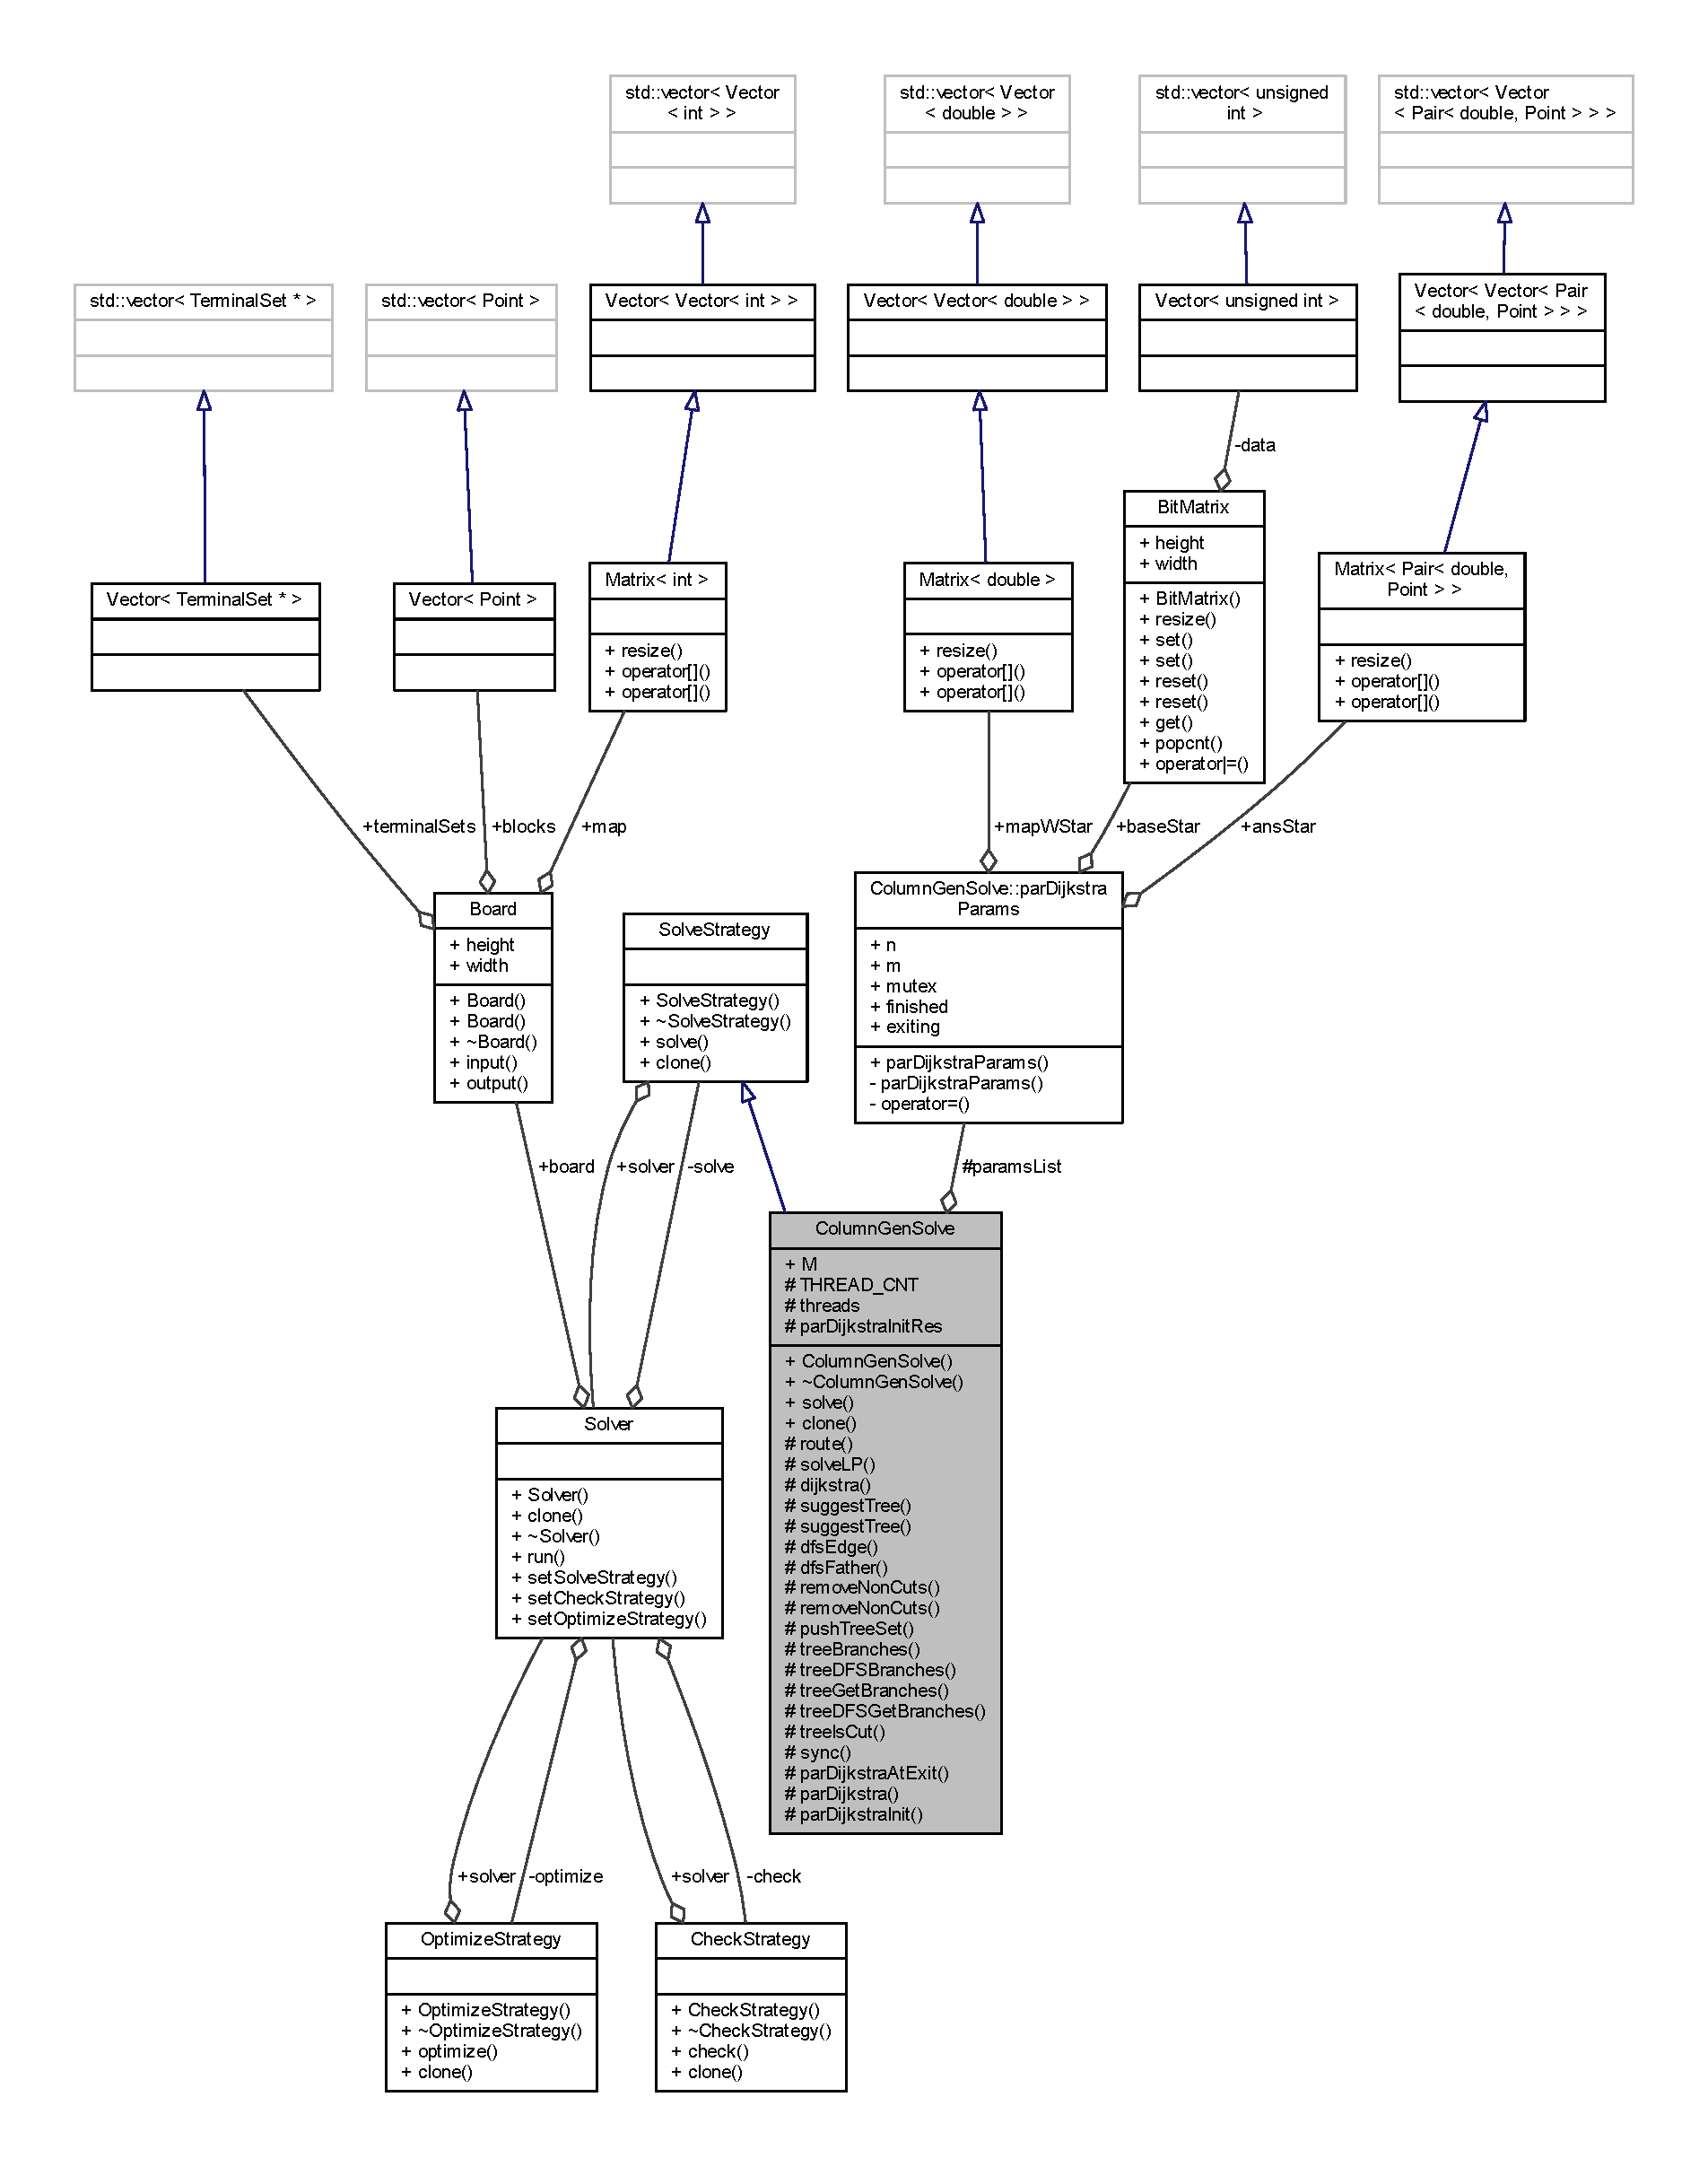
\includegraphics[width=350pt]{classColumnGenSolve__coll__graph}
\end{center}
\end{figure}
\subsection*{类}
\begin{DoxyCompactItemize}
\item 
struct \hyperlink{structColumnGenSolve_1_1expandFinished}{expand\+Finished}
\item 
struct \hyperlink{structColumnGenSolve_1_1parDijkstraParams}{par\+Dijkstra\+Params}
\end{DoxyCompactItemize}
\subsection*{Public 成员函数}
\begin{DoxyCompactItemize}
\item 
\hyperlink{classColumnGenSolve_a825d4a3f8f1995c6a772535b29b3bbeb}{Column\+Gen\+Solve} (\hyperlink{classSolver}{Solver} $\ast$solver\+\_\+)
\item 
virtual \hyperlink{classColumnGenSolve_a04ccfc4d9676794aa5413590b41a07f4}{$\sim$\+Column\+Gen\+Solve} ()
\item 
virtual \hyperlink{classSolution}{Solution} \hyperlink{classColumnGenSolve_aad7c316627e7ea6de4138db1a33e66ee}{solve} () const 
\item 
virtual \hyperlink{classSolveStrategy}{Solve\+Strategy} $\ast$ \hyperlink{classColumnGenSolve_ae7cc479a554a497f738630259e446b8f}{clone} () const 
\end{DoxyCompactItemize}
\subsection*{Public 属性}
\begin{DoxyCompactItemize}
\item 
const double \hyperlink{classColumnGenSolve_ac5abb4d6dfd291b01af6ea006b5f9f5d}{M}
\end{DoxyCompactItemize}
\subsection*{Protected 成员函数}
\begin{DoxyCompactItemize}
\item 
\hyperlink{classVector}{Vector}$<$ \hyperlink{classTree}{Tree} $\ast$ $>$ \hyperlink{classColumnGenSolve_af97cd5f1c4a7305b72e46971fdb85002}{route} (int tim) const 
\item 
double \hyperlink{classColumnGenSolve_aadb23efa531a3eb68651ba11f4d36c81}{solve\+LP} (\hyperlink{classVector}{Vector}$<$ \hyperlink{classVector}{Vector}$<$ \hyperlink{classPair}{Pair}$<$ \hyperlink{classTree}{Tree}, \hyperlink{classGRBVar}{G\+R\+B\+Var} $>$$>$$>$ \&treesets, int mode, \hyperlink{classMatrix}{Matrix}$<$ double $>$ $\ast$map\+Pi=N\+U\+LL, \hyperlink{classVector}{Vector}$<$ double $>$ $\ast$vec\+Lambda=N\+U\+LL, int ignore\+Idx=-\/1) const 
\item 
void \hyperlink{classColumnGenSolve_a71007959556061091171c03da6197f34}{dijkstra} (const \hyperlink{classBitMatrix}{Bit\+Matrix} \&base, const \hyperlink{classMatrix}{Matrix}$<$ double $>$ \&mapW, int n, int m, \hyperlink{classMatrix}{Matrix}$<$ \hyperlink{classPair}{Pair}$<$ double, \hyperlink{classPoint}{Point} $>$$>$ \&ans) const 
\item 
bool \hyperlink{classColumnGenSolve_a4ec729b2184612495e657f7ec2d644fa}{suggest\+Tree} (const \hyperlink{classVector}{Vector}$<$ \hyperlink{classTerminalSet}{Terminal\+Set} $\ast$ $>$ \&termsets, \hyperlink{classVector}{Vector}$<$ \hyperlink{classVector}{Vector}$<$ \hyperlink{classPair}{Pair}$<$ \hyperlink{classTree}{Tree}, \hyperlink{classGRBVar}{G\+R\+B\+Var} $>$$>$$>$ \&treesets, const \hyperlink{classMatrix}{Matrix}$<$ double $>$ \&mapW, int n, int m, int idx) const 
\item 
\hyperlink{classTree}{Tree} \hyperlink{classColumnGenSolve_a9f9ca7d65c0e42d18ea422ff136d52d0}{suggest\+Tree} (const \hyperlink{classTerminalSet}{Terminal\+Set} $\ast$\hyperlink{classes_8txt_a597568d74a60fa533165215be11d5f0b}{terminal\+Set}, const \hyperlink{classMatrix}{Matrix}$<$ double $>$ \&mapW, int n, int m) const 
\item 
void \hyperlink{classColumnGenSolve_a96cbeba5fb978bb67e32b8f42ba161fe}{dfs\+Edge} (\hyperlink{classBitMatrix}{Bit\+Matrix} \&tree, const \hyperlink{classMatrix}{Matrix}$<$ int $>$ \&\hyperlink{classes_8txt_a7441ef0865bcb3db9b8064dd7375c1ea}{id}, \hyperlink{classVector}{Vector}$<$ \hyperlink{classPoint}{Point} $>$ \&\hyperlink{classes_8txt_ae368e6252d0add75ea011d5d90db68ed}{points}, int x, int \hyperlink{classes_8txt_a52673b1e0cce0104e52dcd12727f211e}{y}, int n, int m, int \&s, int \&t) const 
\item 
int \hyperlink{classColumnGenSolve_af3470aaed4b9d0aa92f27b487b093479}{dfs\+Father} (\hyperlink{classVector}{Vector}$<$ int $>$ \&father, int x) const 
\item 
void \hyperlink{classColumnGenSolve_a6c08d317e692a357d49ee56184a9db22}{remove\+Non\+Cuts} (const \hyperlink{classMatrix}{Matrix}$<$ int $>$ \&\hyperlink{classes_8txt_a0a12e395730487ab04f7f11cbc4d2132}{map}, int idx, \hyperlink{classBitMatrix}{Bit\+Matrix} \&tree, int n, int m, const \hyperlink{classMatrix}{Matrix}$<$ double $>$ $\ast$mapW=N\+U\+LL) const 
\item 
double \hyperlink{classColumnGenSolve_ad5a36333d83b1a1803eb582c9a0a9941}{remove\+Non\+Cuts} (\hyperlink{classMatrix}{Matrix}$<$ bool $>$ \&visited, const \hyperlink{classMatrix}{Matrix}$<$ int $>$ \&\hyperlink{classes_8txt_a0a12e395730487ab04f7f11cbc4d2132}{map}, int idx, const \hyperlink{classMatrix}{Matrix}$<$ double $>$ \&mapW, \hyperlink{classBitMatrix}{Bit\+Matrix} \&tree, int n, int m) const 
\item 
bool \hyperlink{classColumnGenSolve_a4a1019de523004757e60c023fc92a38d}{push\+Tree\+Set} (\hyperlink{classVector}{Vector}$<$ \hyperlink{classPair}{Pair}$<$ \hyperlink{classTree}{Tree}, \hyperlink{classGRBVar}{G\+R\+B\+Var} $>$$>$ \&treeset, \hyperlink{classTree}{Tree} \&tree) const 
\item 
int \hyperlink{classColumnGenSolve_ac6a085a6c1704afde58891f19d1acf78}{tree\+Branches} (\hyperlink{classBitMatrix}{Bit\+Matrix} tree, int n, int m) const 
\item 
void \hyperlink{classColumnGenSolve_a57004ff3ac6bffa4f19fa5838a851a25}{tree\+D\+F\+S\+Branches} (\hyperlink{classBitMatrix}{Bit\+Matrix} \&tree, int i, int j, int n, int m) const 
\item 
\hyperlink{classVector}{Vector}$<$ \hyperlink{classBitMatrix}{Bit\+Matrix} $>$ \hyperlink{classColumnGenSolve_acbcc78e94e4a6e59ceb7da2357ddb87a}{tree\+Get\+Branches} (\hyperlink{classBitMatrix}{Bit\+Matrix} tree, int n, int m) const 
\item 
void \hyperlink{classColumnGenSolve_a39be14a210fccecb512a754e1a359861}{tree\+D\+F\+S\+Get\+Branches} (\hyperlink{classBitMatrix}{Bit\+Matrix} \&tree, \hyperlink{classBitMatrix}{Bit\+Matrix} \&res, int i, int j, int n, int m) const 
\item 
bool \hyperlink{classColumnGenSolve_ae971ef7c0098fd33bea1701fbfe92f4f}{tree\+Is\+Cut} (\hyperlink{classBitMatrix}{Bit\+Matrix} tree, int i, int j, int n, int m) const 
\end{DoxyCompactItemize}
\subsection*{静态 Protected 成员函数}
\begin{DoxyCompactItemize}
\item 
static void \hyperlink{classColumnGenSolve_ab976cab8582808218110d86252177f88}{sync} ()
\item 
static void \hyperlink{classColumnGenSolve_a5501879ba2b6480f0bacbc38b6e5121e}{par\+Dijkstra\+At\+Exit} ()
\item 
static void \hyperlink{classColumnGenSolve_a6dc294df38e9aa3160f435bd527f2f20}{par\+Dijkstra} (\hyperlink{structColumnGenSolve_1_1parDijkstraParams}{par\+Dijkstra\+Params} \&params)
\item 
static void $\ast$ \hyperlink{classColumnGenSolve_a97e581fdab12a396fd173b030ec26bec}{par\+Dijkstra\+Init} ()
\end{DoxyCompactItemize}
\subsection*{静态 Protected 属性}
\begin{DoxyCompactItemize}
\item 
static const int \hyperlink{classColumnGenSolve_a6ead284bdba22a11e3b84eb873807e23}{T\+H\+R\+E\+A\+D\+\_\+\+C\+NT} = 2
\item 
static \hyperlink{global_8h_ab4108db709b91dc2efcd48309edb9f5e}{Thread} \hyperlink{classColumnGenSolve_ae836bca68776f265a26e46c7e842492e}{threads} \mbox{[}\hyperlink{classColumnGenSolve_a6ead284bdba22a11e3b84eb873807e23}{T\+H\+R\+E\+A\+D\+\_\+\+C\+NT}\mbox{]}
\item 
static \hyperlink{structColumnGenSolve_1_1parDijkstraParams}{par\+Dijkstra\+Params} \hyperlink{classColumnGenSolve_aba2e5f0dc752db74718e834faf9ef606}{params\+List} \mbox{[}\hyperlink{classColumnGenSolve_a6ead284bdba22a11e3b84eb873807e23}{T\+H\+R\+E\+A\+D\+\_\+\+C\+NT}\mbox{]}
\item 
static const void $\ast$ \hyperlink{classColumnGenSolve_ac77eb4def69a3476015487be8a49818a}{par\+Dijkstra\+Init\+Res} = \hyperlink{classColumnGenSolve_a97e581fdab12a396fd173b030ec26bec}{Column\+Gen\+Solve\+::par\+Dijkstra\+Init}()
\end{DoxyCompactItemize}


\subsection{详细描述}


在文件 Column\+Gen\+Solve.\+h 第 8 行定义.



\subsection{构造及析构函数说明}
\index{Column\+Gen\+Solve@{Column\+Gen\+Solve}!Column\+Gen\+Solve@{Column\+Gen\+Solve}}
\index{Column\+Gen\+Solve@{Column\+Gen\+Solve}!Column\+Gen\+Solve@{Column\+Gen\+Solve}}
\subsubsection[{\texorpdfstring{Column\+Gen\+Solve(\+Solver $\ast$solver\+\_\+)}{ColumnGenSolve(Solver *solver_)}}]{\setlength{\rightskip}{0pt plus 5cm}Column\+Gen\+Solve\+::\+Column\+Gen\+Solve (
\begin{DoxyParamCaption}
\item[{{\bf Solver} $\ast$}]{solver\+\_\+}
\end{DoxyParamCaption}
)\hspace{0.3cm}{\ttfamily [inline]}}\hypertarget{classColumnGenSolve_a825d4a3f8f1995c6a772535b29b3bbeb}{}\label{classColumnGenSolve_a825d4a3f8f1995c6a772535b29b3bbeb}


在文件 Column\+Gen\+Solve.\+h 第 12 行定义.



参考自 clone().


\begin{DoxyCode}
12 : \hyperlink{classSolveStrategy_adae0995ba06bc3bd6d79b08f7a0677b7}{SolveStrategy}(solver\_), \hyperlink{classColumnGenSolve_ac5abb4d6dfd291b01af6ea006b5f9f5d}{M}(solver\_->\hyperlink{classSolver_a8966a22c2f247addc8ce453d119bc54e}{board}->\hyperlink{classBoard_a90a8efaa4736af25511ac948bdd27d6c}{width} * solver\_->
      \hyperlink{classSolver_a8966a22c2f247addc8ce453d119bc54e}{board}->\hyperlink{classBoard_aa0cb8de0254520dc08dab5796643c8e5}{height})\{\}
\end{DoxyCode}


这是这个函数的调用关系图\+:
\nopagebreak
\begin{figure}[H]
\begin{center}
\leavevmode
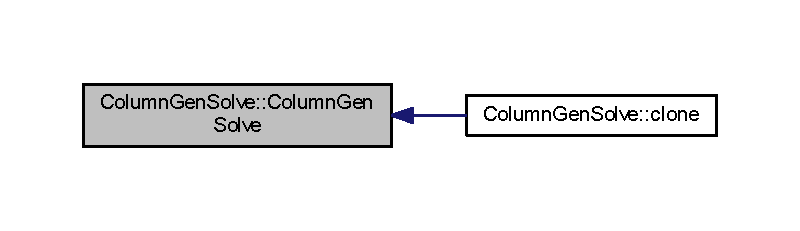
\includegraphics[width=350pt]{classColumnGenSolve_a825d4a3f8f1995c6a772535b29b3bbeb_icgraph}
\end{center}
\end{figure}


\index{Column\+Gen\+Solve@{Column\+Gen\+Solve}!````~Column\+Gen\+Solve@{$\sim$\+Column\+Gen\+Solve}}
\index{````~Column\+Gen\+Solve@{$\sim$\+Column\+Gen\+Solve}!Column\+Gen\+Solve@{Column\+Gen\+Solve}}
\subsubsection[{\texorpdfstring{$\sim$\+Column\+Gen\+Solve()}{~ColumnGenSolve()}}]{\setlength{\rightskip}{0pt plus 5cm}virtual Column\+Gen\+Solve\+::$\sim$\+Column\+Gen\+Solve (
\begin{DoxyParamCaption}
{}
\end{DoxyParamCaption}
)\hspace{0.3cm}{\ttfamily [inline]}, {\ttfamily [virtual]}}\hypertarget{classColumnGenSolve_a04ccfc4d9676794aa5413590b41a07f4}{}\label{classColumnGenSolve_a04ccfc4d9676794aa5413590b41a07f4}


在文件 Column\+Gen\+Solve.\+h 第 13 行定义.



参考 solve().


\begin{DoxyCode}
13 \{\}
\end{DoxyCode}


函数调用图\+:
\nopagebreak
\begin{figure}[H]
\begin{center}
\leavevmode
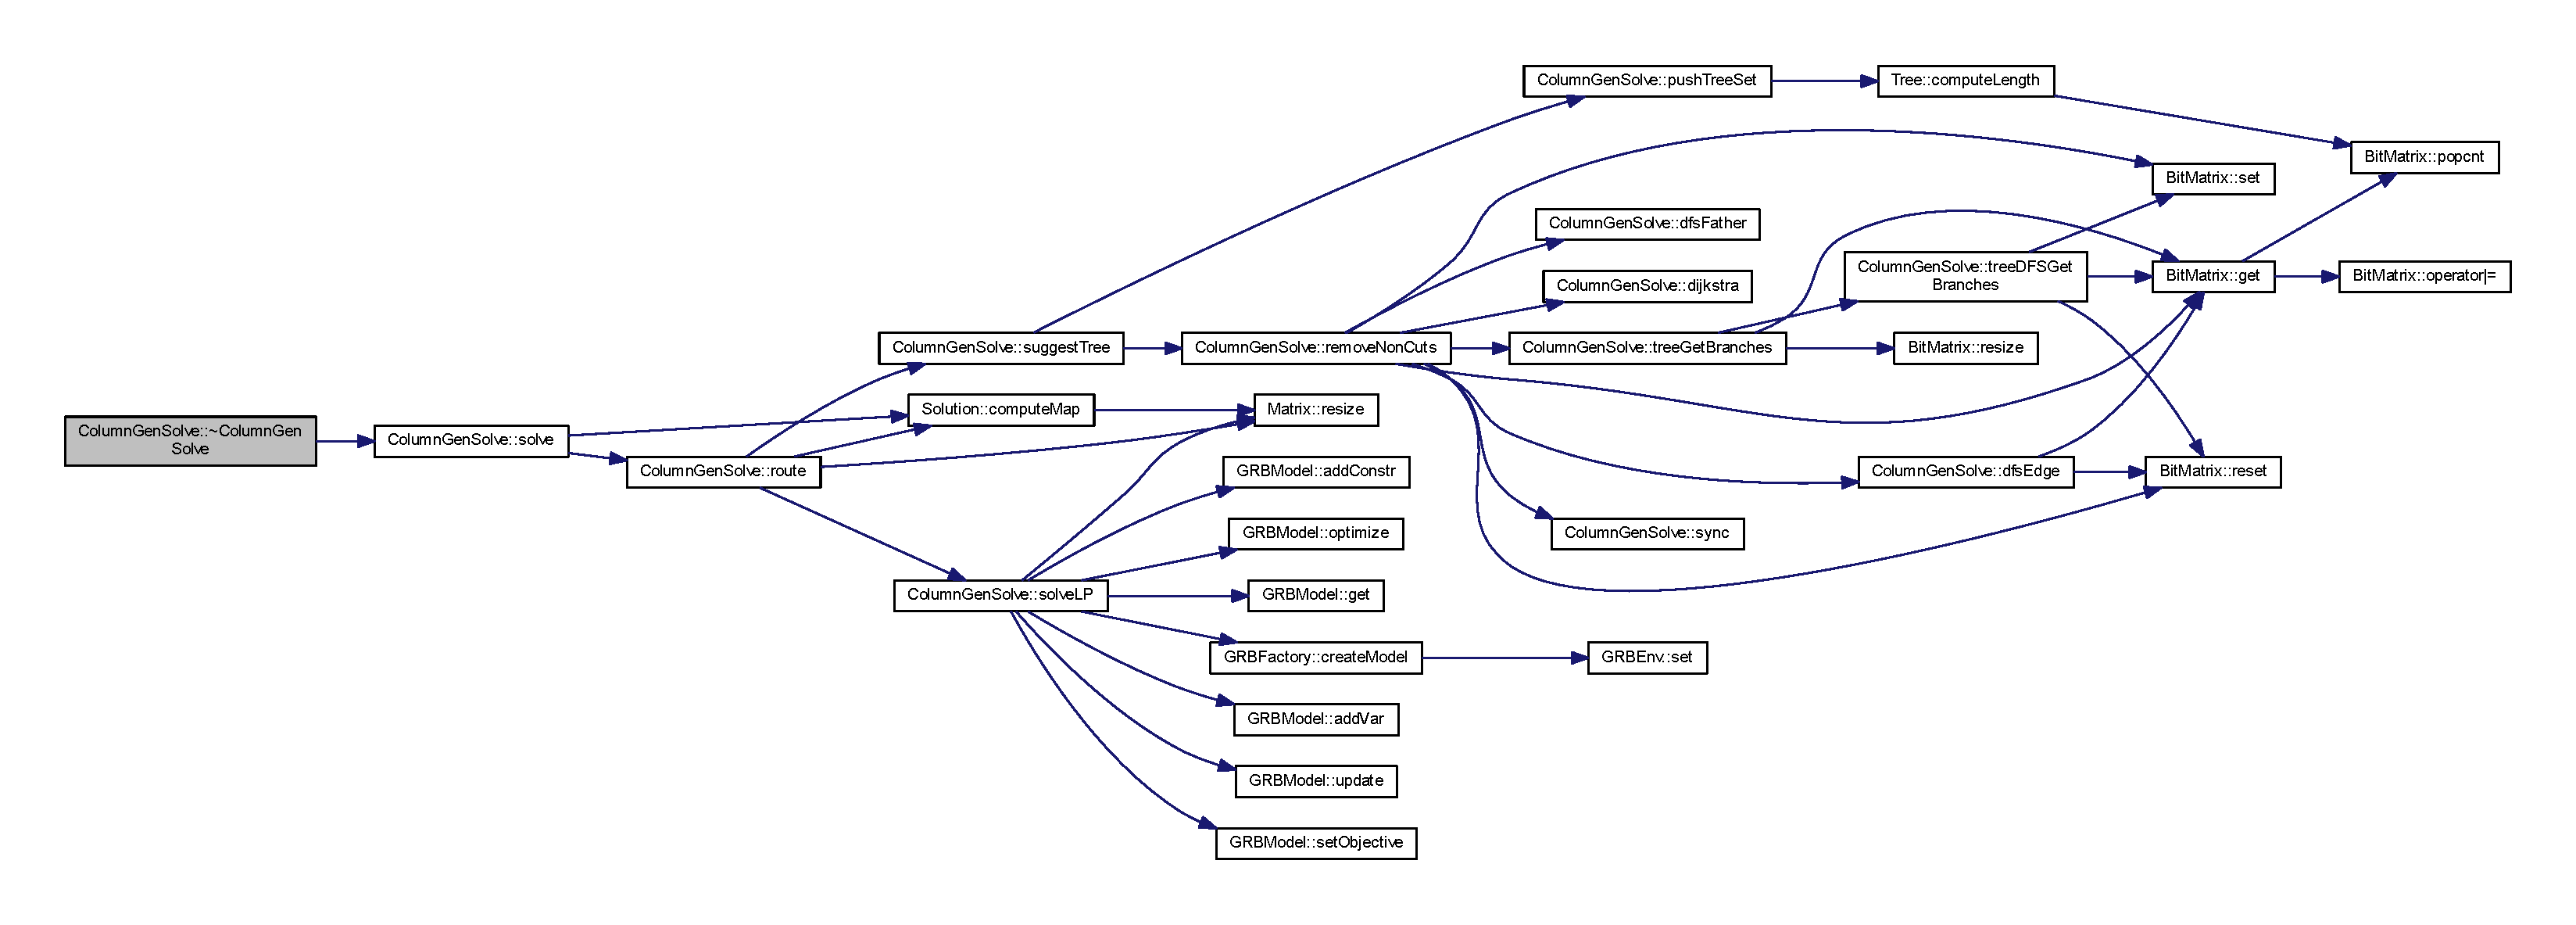
\includegraphics[width=350pt]{classColumnGenSolve_a04ccfc4d9676794aa5413590b41a07f4_cgraph}
\end{center}
\end{figure}




\subsection{成员函数说明}
\index{Column\+Gen\+Solve@{Column\+Gen\+Solve}!clone@{clone}}
\index{clone@{clone}!Column\+Gen\+Solve@{Column\+Gen\+Solve}}
\subsubsection[{\texorpdfstring{clone() const }{clone() const }}]{\setlength{\rightskip}{0pt plus 5cm}virtual {\bf Solve\+Strategy}$\ast$ Column\+Gen\+Solve\+::clone (
\begin{DoxyParamCaption}
{}
\end{DoxyParamCaption}
) const\hspace{0.3cm}{\ttfamily [inline]}, {\ttfamily [virtual]}}\hypertarget{classColumnGenSolve_ae7cc479a554a497f738630259e446b8f}{}\label{classColumnGenSolve_ae7cc479a554a497f738630259e446b8f}


实现了 \hyperlink{classSolveStrategy_a49d51ab69b0c47648638819c2f61f247}{Solve\+Strategy}.



在文件 Column\+Gen\+Solve.\+h 第 15 行定义.



参考 Column\+Gen\+Solve().


\begin{DoxyCode}
16     \{
17         \textcolor{keywordflow}{return} \textcolor{keyword}{new} \hyperlink{classColumnGenSolve_a825d4a3f8f1995c6a772535b29b3bbeb}{ColumnGenSolve}(*\textcolor{keyword}{this});
18     \}
\end{DoxyCode}


函数调用图\+:
\nopagebreak
\begin{figure}[H]
\begin{center}
\leavevmode
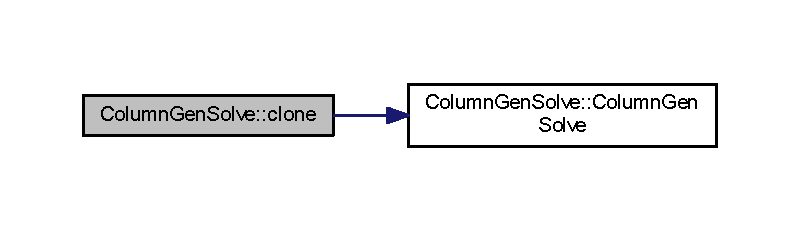
\includegraphics[width=350pt]{classColumnGenSolve_ae7cc479a554a497f738630259e446b8f_cgraph}
\end{center}
\end{figure}


\index{Column\+Gen\+Solve@{Column\+Gen\+Solve}!dfs\+Edge@{dfs\+Edge}}
\index{dfs\+Edge@{dfs\+Edge}!Column\+Gen\+Solve@{Column\+Gen\+Solve}}
\subsubsection[{\texorpdfstring{dfs\+Edge(\+Bit\+Matrix \&tree, const Matrix$<$ int $>$ \&id, Vector$<$ Point $>$ \&points, int x, int y, int n, int m, int \&s, int \&t) const }{dfsEdge(BitMatrix &tree, const Matrix< int > &id, Vector< Point > &points, int x, int y, int n, int m, int &s, int &t) const }}]{\setlength{\rightskip}{0pt plus 5cm}void Column\+Gen\+Solve\+::dfs\+Edge (
\begin{DoxyParamCaption}
\item[{{\bf Bit\+Matrix} \&}]{tree, }
\item[{const {\bf Matrix}$<$ int $>$ \&}]{id, }
\item[{{\bf Vector}$<$ {\bf Point} $>$ \&}]{points, }
\item[{int}]{x, }
\item[{int}]{y, }
\item[{int}]{n, }
\item[{int}]{m, }
\item[{int \&}]{s, }
\item[{int \&}]{t}
\end{DoxyParamCaption}
) const\hspace{0.3cm}{\ttfamily [protected]}}\hypertarget{classColumnGenSolve_a96cbeba5fb978bb67e32b8f42ba161fe}{}\label{classColumnGenSolve_a96cbeba5fb978bb67e32b8f42ba161fe}


在文件 Column\+Gen\+Solve.\+cpp 第 762 行定义.



参考 assert, Bit\+Matrix\+::get(), Bit\+Matrix\+::reset() , 以及 y.



参考自 remove\+Non\+Cuts().


\begin{DoxyCode}
766 \{
767     \textcolor{keywordflow}{if}(x < 0 || x >= n || y < 0 || y >= m || !tree.\hyperlink{classBitMatrix_ad19d1045b54ccc8a99d70d38305b4ca6}{get}(x, \hyperlink{classes_8txt_a52673b1e0cce0104e52dcd12727f211e}{y}))
768         \textcolor{keywordflow}{return};
769     \textcolor{keywordflow}{if}(\textcolor{keywordtype}{id}[x][\hyperlink{classes_8txt_a52673b1e0cce0104e52dcd12727f211e}{y}])
770     \{
771         \textcolor{keywordflow}{if}(s)
772         \{
773             \hyperlink{global_8h_af576bf8ffa22a44e53018c67095ffbf0}{assert}(!t);
774             t = \textcolor{keywordtype}{id}[x][\hyperlink{classes_8txt_a52673b1e0cce0104e52dcd12727f211e}{y}];
775         \}
776         \textcolor{keywordflow}{else}
777             s = \textcolor{keywordtype}{id}[x][\hyperlink{classes_8txt_a52673b1e0cce0104e52dcd12727f211e}{y}];
778         \textcolor{keywordflow}{return};
779     \}
780     points.push\_back(\hyperlink{classPoint}{Point}(x, y));
781     tree.\hyperlink{classBitMatrix_a0ee870454e6343c3272ab791e45af404}{reset}(x, y);
782     \hyperlink{classColumnGenSolve_a96cbeba5fb978bb67e32b8f42ba161fe}{dfsEdge}(tree, \textcolor{keywordtype}{id}, points, x - 1, y, n, m, s, t);
783     \hyperlink{classColumnGenSolve_a96cbeba5fb978bb67e32b8f42ba161fe}{dfsEdge}(tree, \textcolor{keywordtype}{id}, points, x + 1, y, n, m, s, t);
784     \hyperlink{classColumnGenSolve_a96cbeba5fb978bb67e32b8f42ba161fe}{dfsEdge}(tree, \textcolor{keywordtype}{id}, points, x, y - 1, n, m, s, t);
785     \hyperlink{classColumnGenSolve_a96cbeba5fb978bb67e32b8f42ba161fe}{dfsEdge}(tree, \textcolor{keywordtype}{id}, points, x, y + 1, n, m, s, t);
786 \}
\end{DoxyCode}


函数调用图\+:
\nopagebreak
\begin{figure}[H]
\begin{center}
\leavevmode
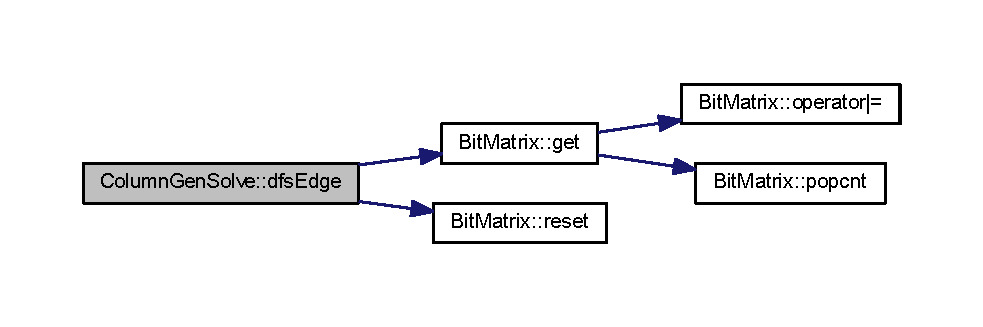
\includegraphics[width=350pt]{classColumnGenSolve_a96cbeba5fb978bb67e32b8f42ba161fe_cgraph}
\end{center}
\end{figure}




这是这个函数的调用关系图\+:
\nopagebreak
\begin{figure}[H]
\begin{center}
\leavevmode
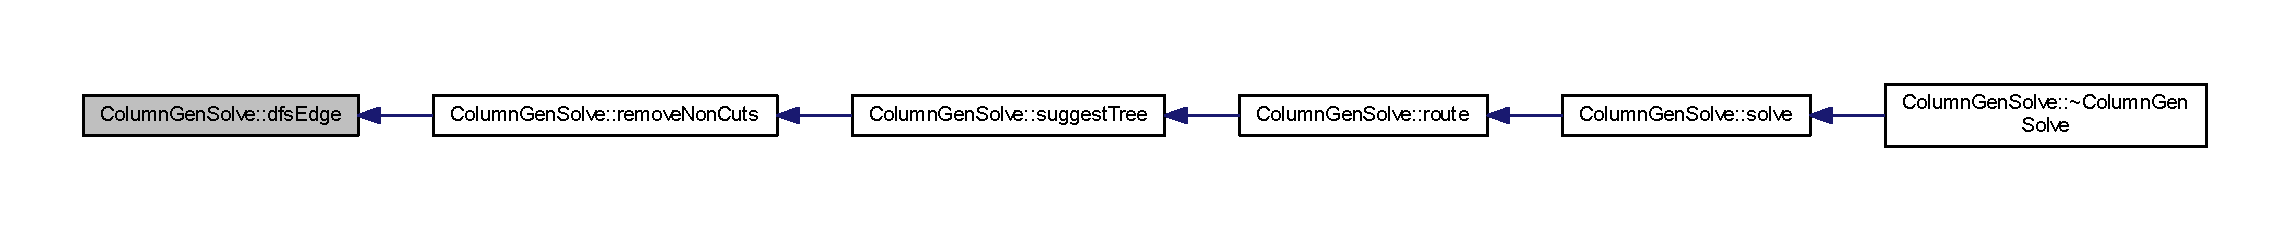
\includegraphics[width=350pt]{classColumnGenSolve_a96cbeba5fb978bb67e32b8f42ba161fe_icgraph}
\end{center}
\end{figure}


\index{Column\+Gen\+Solve@{Column\+Gen\+Solve}!dfs\+Father@{dfs\+Father}}
\index{dfs\+Father@{dfs\+Father}!Column\+Gen\+Solve@{Column\+Gen\+Solve}}
\subsubsection[{\texorpdfstring{dfs\+Father(\+Vector$<$ int $>$ \&father, int x) const }{dfsFather(Vector< int > &father, int x) const }}]{\setlength{\rightskip}{0pt plus 5cm}int Column\+Gen\+Solve\+::dfs\+Father (
\begin{DoxyParamCaption}
\item[{{\bf Vector}$<$ int $>$ \&}]{father, }
\item[{int}]{x}
\end{DoxyParamCaption}
) const\hspace{0.3cm}{\ttfamily [protected]}}\hypertarget{classColumnGenSolve_af3470aaed4b9d0aa92f27b487b093479}{}\label{classColumnGenSolve_af3470aaed4b9d0aa92f27b487b093479}


在文件 Column\+Gen\+Solve.\+cpp 第 788 行定义.



参考自 remove\+Non\+Cuts().


\begin{DoxyCode}
789 \{
790     \textcolor{keywordflow}{if}(father[x] == x)
791         \textcolor{keywordflow}{return} x;
792     \textcolor{keywordflow}{else}
793         \textcolor{keywordflow}{return} father[x] = \hyperlink{classColumnGenSolve_af3470aaed4b9d0aa92f27b487b093479}{dfsFather}(father, father[x]);
794 \}
\end{DoxyCode}


这是这个函数的调用关系图\+:
\nopagebreak
\begin{figure}[H]
\begin{center}
\leavevmode
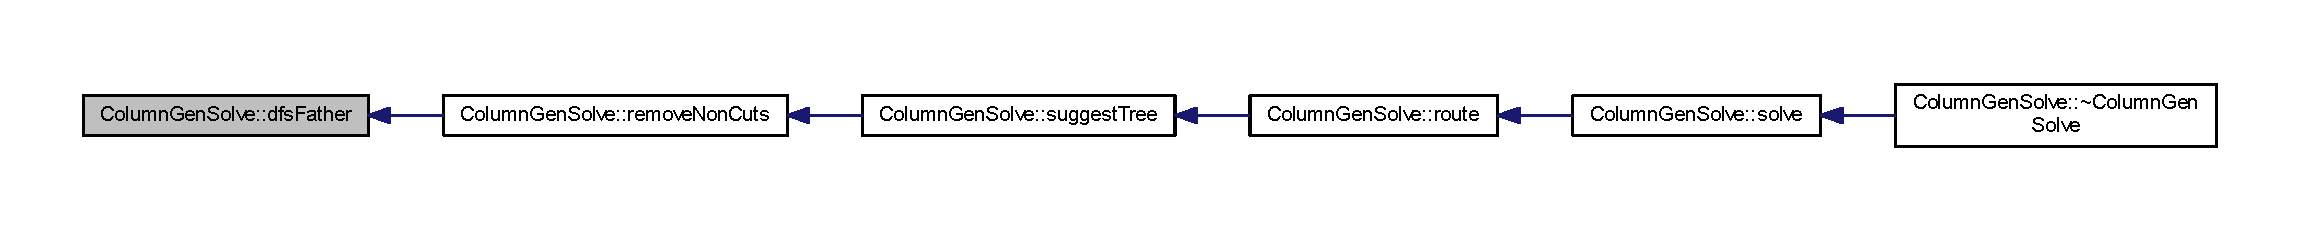
\includegraphics[width=350pt]{classColumnGenSolve_af3470aaed4b9d0aa92f27b487b093479_icgraph}
\end{center}
\end{figure}


\index{Column\+Gen\+Solve@{Column\+Gen\+Solve}!dijkstra@{dijkstra}}
\index{dijkstra@{dijkstra}!Column\+Gen\+Solve@{Column\+Gen\+Solve}}
\subsubsection[{\texorpdfstring{dijkstra(const Bit\+Matrix \&base, const Matrix$<$ double $>$ \&map\+W, int n, int m, Matrix$<$ Pair$<$ double, Point $>$$>$ \&ans) const }{dijkstra(const BitMatrix &base, const Matrix< double > &mapW, int n, int m, Matrix< Pair< double, Point >> &ans) const }}]{\setlength{\rightskip}{0pt plus 5cm}void Column\+Gen\+Solve\+::dijkstra (
\begin{DoxyParamCaption}
\item[{const {\bf Bit\+Matrix} \&}]{base, }
\item[{const {\bf Matrix}$<$ double $>$ \&}]{mapW, }
\item[{int}]{n, }
\item[{int}]{m, }
\item[{{\bf Matrix}$<$ {\bf Pair}$<$ double, {\bf Point} $>$$>$ \&}]{ans}
\end{DoxyParamCaption}
) const\hspace{0.3cm}{\ttfamily [protected]}}\hypertarget{classColumnGenSolve_a71007959556061091171c03da6197f34}{}\label{classColumnGenSolve_a71007959556061091171c03da6197f34}


在文件 Column\+Gen\+Solve.\+cpp 第 643 行定义.



参考 Column\+Gen\+Solve\+::par\+Dijkstra\+Params\+::ans\+Star, Column\+Gen\+Solve\+::par\+Dijkstra\+Params\+::base\+Star, Column\+Gen\+Solve\+::par\+Dijkstra\+Params\+::finished, id, Column\+Gen\+Solve\+::par\+Dijkstra\+Params\+::m, Column\+Gen\+Solve\+::par\+Dijkstra\+Params\+::map\+W\+Star, Column\+Gen\+Solve\+::par\+Dijkstra\+Params\+::n, params\+List , 以及 T\+H\+R\+E\+A\+D\+\_\+\+C\+NT.



参考自 remove\+Non\+Cuts() , 以及 suggest\+Tree().


\begin{DoxyCode}
647 \{
648     \textcolor{keywordtype}{int} \textcolor{keywordtype}{id} = -1;
649     \textcolor{keywordflow}{for}(;;)
650     \{
651         \textcolor{keywordflow}{for}(\textcolor{keywordtype}{int} i = 0; i < \hyperlink{classColumnGenSolve_a6ead284bdba22a11e3b84eb873807e23}{THREAD\_CNT}; i++)
652             \textcolor{comment}{// if(paramsList[i].mutex.try\_lock())}
653             \textcolor{comment}{// \{}
654                 \textcolor{keywordflow}{if}(\hyperlink{classColumnGenSolve_aba2e5f0dc752db74718e834faf9ef606}{paramsList}[i].finished)
655                 \{
656                     \textcolor{keywordtype}{id} = i;
657                     \textcolor{keywordflow}{goto} foundThread;
658                 \}
659                 \textcolor{comment}{// paramsList[i].mutex.unlock();}
660             \textcolor{comment}{// \}}
661         std::this\_thread::sleep\_for(std::chrono::microseconds(1));
662     \}
663     foundThread:;
664     \textcolor{comment}{// cout << "id = " << id << '\(\backslash\)n';}
665     \textcolor{keyword}{static} \textcolor{keywordtype}{int} a = 0;
666     \textcolor{keyword}{static} \textcolor{keywordtype}{int} b = 0;
667     a += \hyperlink{classes_8txt_a7441ef0865bcb3db9b8064dd7375c1ea}{id}; ++b;
668     \textcolor{comment}{// cout << "p " << a << "/" << b << "\(\backslash\)n";}
669     \textcolor{comment}{// cout.flush();}
670     parDijkstraParams &params = \hyperlink{classColumnGenSolve_aba2e5f0dc752db74718e834faf9ef606}{paramsList}[\hyperlink{classes_8txt_a7441ef0865bcb3db9b8064dd7375c1ea}{id}];
671     params.\hyperlink{structColumnGenSolve_1_1parDijkstraParams_a6d66ec75238960aaf04d2d62058ea077}{baseStar} = &base;
672     params.mapWStar = &mapW;
673     params.n = n; params.m = m;
674     params.ansStar = &ans;
675     \textcolor{comment}{// cout << "createthread begin" << '\(\backslash\)n';}
676     \textcolor{comment}{// cout.flush();}
677     params.finished = \textcolor{keyword}{false};
678     \textcolor{comment}{// cout << "createthread end" << '\(\backslash\)n';}
679     \textcolor{comment}{// cout.flush();}
680     \textcolor{comment}{// params.mutex.unlock();}
681 \}
\end{DoxyCode}


这是这个函数的调用关系图\+:
\nopagebreak
\begin{figure}[H]
\begin{center}
\leavevmode
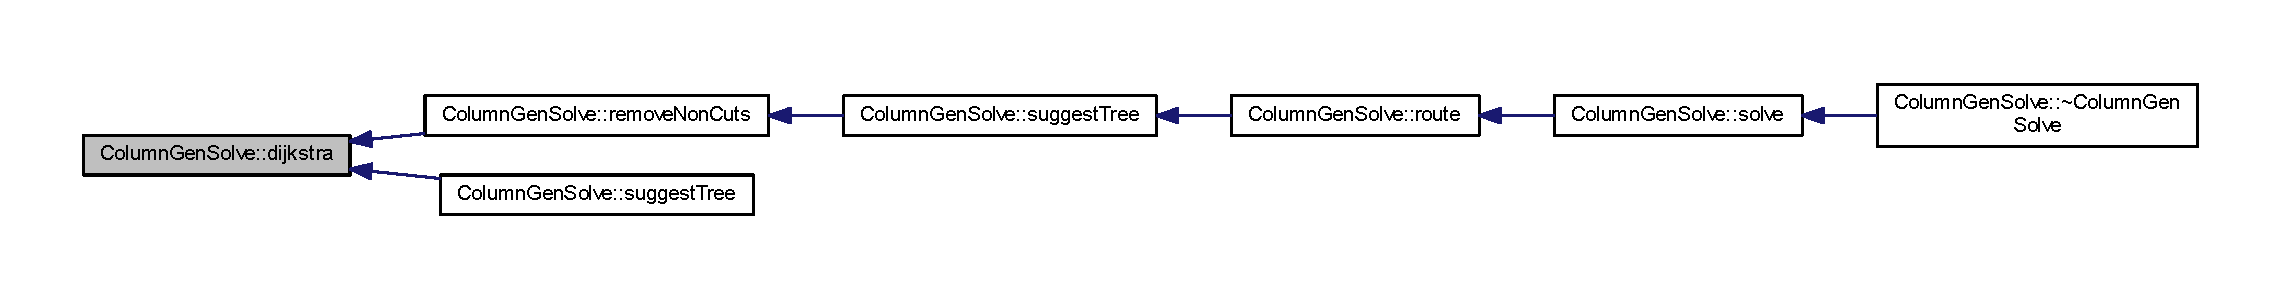
\includegraphics[width=350pt]{classColumnGenSolve_a71007959556061091171c03da6197f34_icgraph}
\end{center}
\end{figure}


\index{Column\+Gen\+Solve@{Column\+Gen\+Solve}!par\+Dijkstra@{par\+Dijkstra}}
\index{par\+Dijkstra@{par\+Dijkstra}!Column\+Gen\+Solve@{Column\+Gen\+Solve}}
\subsubsection[{\texorpdfstring{par\+Dijkstra(par\+Dijkstra\+Params \&params)}{parDijkstra(parDijkstraParams &params)}}]{\setlength{\rightskip}{0pt plus 5cm}void Column\+Gen\+Solve\+::par\+Dijkstra (
\begin{DoxyParamCaption}
\item[{{\bf Column\+Gen\+Solve\+::par\+Dijkstra\+Params} \&}]{params}
\end{DoxyParamCaption}
)\hspace{0.3cm}{\ttfamily [static]}, {\ttfamily [protected]}}\hypertarget{classColumnGenSolve_a6dc294df38e9aa3160f435bd527f2f20}{}\label{classColumnGenSolve_a6dc294df38e9aa3160f435bd527f2f20}


在文件 Column\+Gen\+Solve.\+cpp 第 544 行定义.



参考 Column\+Gen\+Solve\+::par\+Dijkstra\+Params\+::ans\+Star, Column\+Gen\+Solve\+::par\+Dijkstra\+Params\+::base\+Star, Column\+Gen\+Solve\+::par\+Dijkstra\+Params\+::exiting, Column\+Gen\+Solve\+::par\+Dijkstra\+Params\+::finished, Bit\+Matrix\+::get(), Column\+Gen\+Solve\+::par\+Dijkstra\+Params\+::m, Column\+Gen\+Solve\+::par\+Dijkstra\+Params\+::map\+W\+Star, Column\+Gen\+Solve\+::par\+Dijkstra\+Params\+::n , 以及 Matrix$<$ T $>$\+::resize().



参考自 par\+Dijkstra\+Init().


\begin{DoxyCode}
545 \{
546     \textcolor{keywordflow}{for}(;;)
547     \{
548         \textcolor{comment}{// params.mutex.lock();}
549         \textcolor{keywordflow}{if}(params.\hyperlink{structColumnGenSolve_1_1parDijkstraParams_a56efc1b9b760d7a8934f06406e2e61a0}{exiting})
550             \textcolor{keywordflow}{return};
551         \textcolor{keywordflow}{if}(params.\hyperlink{structColumnGenSolve_1_1parDijkstraParams_a72bfc9f9b0c4851bdb63715b053df511}{finished})
552         \{
553             \textcolor{comment}{// std::this\_thread::sleep\_for(std::chrono::microseconds(1));}
554             \textcolor{comment}{// params.mutex.unlock();}
555             \textcolor{keywordflow}{continue};
556         \}
557         \textcolor{comment}{// cout << "run!\(\backslash\)n";}
558         \textcolor{comment}{// cout.flush();}
559         \textcolor{keyword}{const} \hyperlink{classBitMatrix}{BitMatrix} &base = *params.\hyperlink{structColumnGenSolve_1_1parDijkstraParams_a6d66ec75238960aaf04d2d62058ea077}{baseStar};
560         \textcolor{keyword}{const} \hyperlink{classMatrix}{Matrix<double>} &mapW = *params.\hyperlink{structColumnGenSolve_1_1parDijkstraParams_ae0b35a1ba11e00c8ce3113b2a174042d}{mapWStar};
561         \textcolor{keywordtype}{int} n = params.\hyperlink{structColumnGenSolve_1_1parDijkstraParams_a33cbd8316dde8102d996c01ad2ae68d5}{n}, m = params.\hyperlink{structColumnGenSolve_1_1parDijkstraParams_a20f153fdd04ede56c8ec19f155e1e423}{m};
562         \hyperlink{classMatrix}{Matrix<Pair<double, Point>}> &ans = *params.
      \hyperlink{structColumnGenSolve_1_1parDijkstraParams_a6e3c1462f7a9a1714c190a83819cf632}{ansStar};
563         \textcolor{comment}{// simple Dijkstra algorithm}
564         \hyperlink{classMatrix}{Matrix<Pair<double, Point>}> dist;
565         dist.\hyperlink{classMatrix_a15ce96c8af4c7a982c2c10b96f29cea1}{resize}(n, m);
566         \textcolor{keywordflow}{for}(\textcolor{keywordtype}{int} i = 0; i < n; i++)
567             \textcolor{keywordflow}{for}(\textcolor{keywordtype}{int} j = 0; j < m; j++)
568                 \textcolor{keywordflow}{if}(base.\hyperlink{classBitMatrix_ad19d1045b54ccc8a99d70d38305b4ca6}{get}(i, j))
569                     dist[i][j].second = \hyperlink{classPoint}{Point}(-1, -1);
570                 \textcolor{keywordflow}{else}
571                     dist[i][j].first = 1e30;
572         \textcolor{comment}{// Matrix<bool> visited;}
573         \textcolor{comment}{// visited.resize(n, m);}
574         \textcolor{keywordtype}{int} dx[4] = \{1, -1, 0, 0\};
575         \textcolor{keywordtype}{int} dy[4] = \{0, 0, 1, -1\};
576         \textcolor{keywordtype}{int} EX = 1;
577         \textcolor{keywordflow}{while}(n * m > EX)
578             EX <<= 1;
579         vector<double> sgt;
580         sgt.\hyperlink{classMatrix_a15ce96c8af4c7a982c2c10b96f29cea1}{resize}(EX << 1, 1e30);
581         \textcolor{keywordflow}{for}(\textcolor{keywordtype}{int} i = 0; i < n; i++)
582             \textcolor{keywordflow}{for}(\textcolor{keywordtype}{int} j = 0; j < m; j++)
583                 \textcolor{keywordflow}{if}(base.\hyperlink{classBitMatrix_ad19d1045b54ccc8a99d70d38305b4ca6}{get}(i, j))
584                     sgt[EX + i * m + j] = 0;
585         \textcolor{keywordflow}{for}(\textcolor{keywordtype}{int} i = EX - 1; i >= 1; i--)
586             sgt[i] = min(sgt[i << 1], sgt[i << 1 | 1]);
587         \textcolor{comment}{// cout << "core dij begin\(\backslash\)n";}
588         \textcolor{keywordflow}{for}(;;)
589         \{
590             \textcolor{comment}{// cout << "cur " << sgt[1] << endl;}
591             \textcolor{keywordflow}{if}(sgt[1] >= 1e25) \textcolor{keywordflow}{break};
592             \textcolor{keywordtype}{int} sgtIdx = 1;
593             \textcolor{keywordflow}{while}(sgtIdx < EX)
594                 \textcolor{keywordflow}{if}(sgt[sgtIdx] == sgt[sgtIdx << 1])
595                     sgtIdx <<= 1;
596                 \textcolor{keywordflow}{else}
597                     sgtIdx = (sgtIdx << 1 | 1);
598             sgtIdx -= EX;
599             \textcolor{keywordtype}{int} cx = sgtIdx / m, cy = sgtIdx % m;
600             sgt[sgtIdx += EX] = 1e30;
601             \textcolor{keywordflow}{for}(sgtIdx >>= 1; sgtIdx; sgtIdx >>= 1)
602                 sgt[sgtIdx] = min(sgt[sgtIdx << 1], sgt[sgtIdx << 1 | 1]);
603             \textcolor{comment}{// visited[cx][cy] = 1;}
604             \textcolor{keyword}{const} \hyperlink{classPair}{Pair<double, Point>} &cd = dist[cx][cy];
605             \textcolor{keywordflow}{for}(\textcolor{keywordtype}{int} d = 0; d < 4; d++)
606             \{
607                 \textcolor{keywordtype}{int} tx = cx + dx[d], ty = cy + dy[d];
608                 \textcolor{keywordflow}{if}(tx < 0 || tx >= n || ty < 0 || ty >= m)
609                     \textcolor{keywordflow}{continue};
610                 \textcolor{keywordtype}{double} tdFirst = cd.first + mapW[tx][ty];
611                 \textcolor{keywordflow}{if}(tdFirst < dist[tx][ty].first)
612                 \{
613                     dist[tx][ty].first = tdFirst;
614                     dist[tx][ty].second = \hyperlink{classPoint}{Point}(cx, cy);
615                     sgt[sgtIdx = EX + tx * m + ty] = tdFirst;
616                     \textcolor{keywordflow}{for}(sgtIdx >>= 1; sgtIdx; sgtIdx >>= 1)
617                         sgt[sgtIdx] = min(sgt[sgtIdx << 1], sgt[sgtIdx << 1 | 1]);
618                 \}
619             \}
620         \}
621         \textcolor{comment}{// cout << "core dij end\(\backslash\)n";}
622         ans = dist;
623         \textcolor{keywordflow}{for}(\textcolor{keywordtype}{int} i = 0; i < n; i++)
624             \textcolor{keywordflow}{for}(\textcolor{keywordtype}{int} j = 0; j < m; j++)
625             \{
626                 \textcolor{keywordflow}{for}(\textcolor{keywordtype}{int} d = 3; d >= 0; d--)
627                 \{
628                     \textcolor{keywordtype}{int} tx = i + dx[d], ty = j + dy[d];
629                     \textcolor{keywordflow}{if}(tx < 0 || tx >= n || ty < 0 || ty >= m)
630                         \textcolor{keywordflow}{continue};
631                     \textcolor{keywordflow}{if}(dist[tx][ty].first < ans[i][j].first)
632                     \{
633                         ans[i][j].first = dist[tx][ty].first;
634                         ans[i][j].second = \hyperlink{classPoint}{Point}(tx, ty);
635                     \}
636                 \}
637             \}
638         params.\hyperlink{structColumnGenSolve_1_1parDijkstraParams_a72bfc9f9b0c4851bdb63715b053df511}{finished} = \textcolor{keyword}{true};
639         \textcolor{comment}{// params.mutex.unlock();}
640     \}
641 \}
\end{DoxyCode}


函数调用图\+:
\nopagebreak
\begin{figure}[H]
\begin{center}
\leavevmode
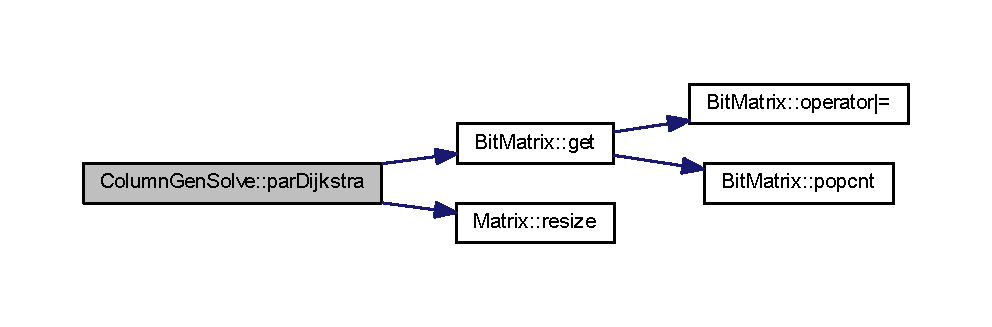
\includegraphics[width=350pt]{classColumnGenSolve_a6dc294df38e9aa3160f435bd527f2f20_cgraph}
\end{center}
\end{figure}




这是这个函数的调用关系图\+:
\nopagebreak
\begin{figure}[H]
\begin{center}
\leavevmode
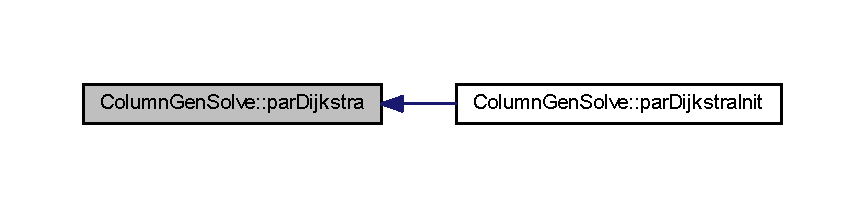
\includegraphics[width=350pt]{classColumnGenSolve_a6dc294df38e9aa3160f435bd527f2f20_icgraph}
\end{center}
\end{figure}


\index{Column\+Gen\+Solve@{Column\+Gen\+Solve}!par\+Dijkstra\+At\+Exit@{par\+Dijkstra\+At\+Exit}}
\index{par\+Dijkstra\+At\+Exit@{par\+Dijkstra\+At\+Exit}!Column\+Gen\+Solve@{Column\+Gen\+Solve}}
\subsubsection[{\texorpdfstring{par\+Dijkstra\+At\+Exit()}{parDijkstraAtExit()}}]{\setlength{\rightskip}{0pt plus 5cm}void Column\+Gen\+Solve\+::par\+Dijkstra\+At\+Exit (
\begin{DoxyParamCaption}
{}
\end{DoxyParamCaption}
)\hspace{0.3cm}{\ttfamily [static]}, {\ttfamily [protected]}}\hypertarget{classColumnGenSolve_a5501879ba2b6480f0bacbc38b6e5121e}{}\label{classColumnGenSolve_a5501879ba2b6480f0bacbc38b6e5121e}


在文件 Column\+Gen\+Solve.\+cpp 第 520 行定义.



参考 Column\+Gen\+Solve\+::par\+Dijkstra\+Params\+::exiting, params\+List, T\+H\+R\+E\+A\+D\+\_\+\+C\+NT , 以及 threads.



参考自 par\+Dijkstra\+Init().


\begin{DoxyCode}
521 \{
522     \textcolor{comment}{// cout << "atexit\(\backslash\)n";}
523     \textcolor{comment}{// cout.flush();}
524     \textcolor{keywordflow}{for}(\textcolor{keywordtype}{int} i = 0; i < \hyperlink{classColumnGenSolve_a6ead284bdba22a11e3b84eb873807e23}{THREAD\_CNT}; i++)\{
525         \hyperlink{classColumnGenSolve_aba2e5f0dc752db74718e834faf9ef606}{paramsList}[i].\hyperlink{structColumnGenSolve_1_1parDijkstraParams_a56efc1b9b760d7a8934f06406e2e61a0}{exiting} = \textcolor{keyword}{true};
526         \hyperlink{classColumnGenSolve_ae836bca68776f265a26e46c7e842492e}{threads}[i].join();
527     \}
528     \textcolor{comment}{// cout << "atexit finished\(\backslash\)n";}
529     \textcolor{comment}{// cout.flush();}
530 \}
\end{DoxyCode}


这是这个函数的调用关系图\+:
\nopagebreak
\begin{figure}[H]
\begin{center}
\leavevmode
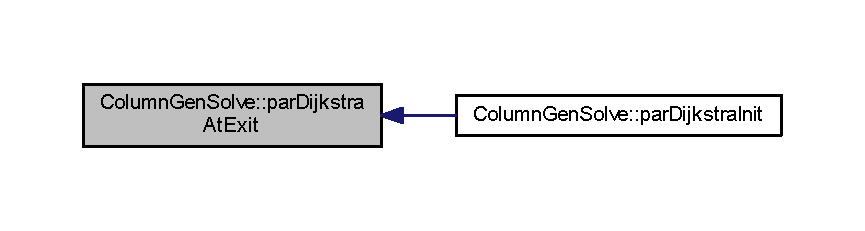
\includegraphics[width=350pt]{classColumnGenSolve_a5501879ba2b6480f0bacbc38b6e5121e_icgraph}
\end{center}
\end{figure}


\index{Column\+Gen\+Solve@{Column\+Gen\+Solve}!par\+Dijkstra\+Init@{par\+Dijkstra\+Init}}
\index{par\+Dijkstra\+Init@{par\+Dijkstra\+Init}!Column\+Gen\+Solve@{Column\+Gen\+Solve}}
\subsubsection[{\texorpdfstring{par\+Dijkstra\+Init()}{parDijkstraInit()}}]{\setlength{\rightskip}{0pt plus 5cm}void $\ast$ Column\+Gen\+Solve\+::par\+Dijkstra\+Init (
\begin{DoxyParamCaption}
{}
\end{DoxyParamCaption}
)\hspace{0.3cm}{\ttfamily [static]}, {\ttfamily [protected]}}\hypertarget{classColumnGenSolve_a97e581fdab12a396fd173b030ec26bec}{}\label{classColumnGenSolve_a97e581fdab12a396fd173b030ec26bec}


在文件 Column\+Gen\+Solve.\+cpp 第 532 行定义.



参考 Column\+Gen\+Solve\+::par\+Dijkstra\+Params\+::exiting, Column\+Gen\+Solve\+::par\+Dijkstra\+Params\+::finished, params\+List, par\+Dijkstra(), par\+Dijkstra\+At\+Exit(), T\+H\+R\+E\+A\+D\+\_\+\+C\+NT , 以及 threads.


\begin{DoxyCode}
533 \{
534     \textcolor{keywordflow}{for}(\textcolor{keywordtype}{int} i = 0; i < \hyperlink{classColumnGenSolve_a6ead284bdba22a11e3b84eb873807e23}{THREAD\_CNT}; i++)
535     \{
536         \hyperlink{classColumnGenSolve_aba2e5f0dc752db74718e834faf9ef606}{paramsList}[i].\hyperlink{structColumnGenSolve_1_1parDijkstraParams_a56efc1b9b760d7a8934f06406e2e61a0}{exiting} = \textcolor{keyword}{false};
537         \hyperlink{classColumnGenSolve_aba2e5f0dc752db74718e834faf9ef606}{paramsList}[i].\hyperlink{structColumnGenSolve_1_1parDijkstraParams_a72bfc9f9b0c4851bdb63715b053df511}{finished} = \textcolor{keyword}{true};
538         \hyperlink{classColumnGenSolve_ae836bca68776f265a26e46c7e842492e}{threads}[i] = \hyperlink{global_8h_ab4108db709b91dc2efcd48309edb9f5e}{Thread}(\hyperlink{classColumnGenSolve_a6dc294df38e9aa3160f435bd527f2f20}{parDijkstra}, std::ref(
      \hyperlink{classColumnGenSolve_aba2e5f0dc752db74718e834faf9ef606}{paramsList}[i]));
539     \}
540     \textcolor{keywordflow}{while}(atexit(\hyperlink{classColumnGenSolve_a5501879ba2b6480f0bacbc38b6e5121e}{ColumnGenSolve::parDijkstraAtExit}));
541     \textcolor{keywordflow}{return} (\textcolor{keywordtype}{void} *) 0x23333333;
542 \}
\end{DoxyCode}


函数调用图\+:
\nopagebreak
\begin{figure}[H]
\begin{center}
\leavevmode
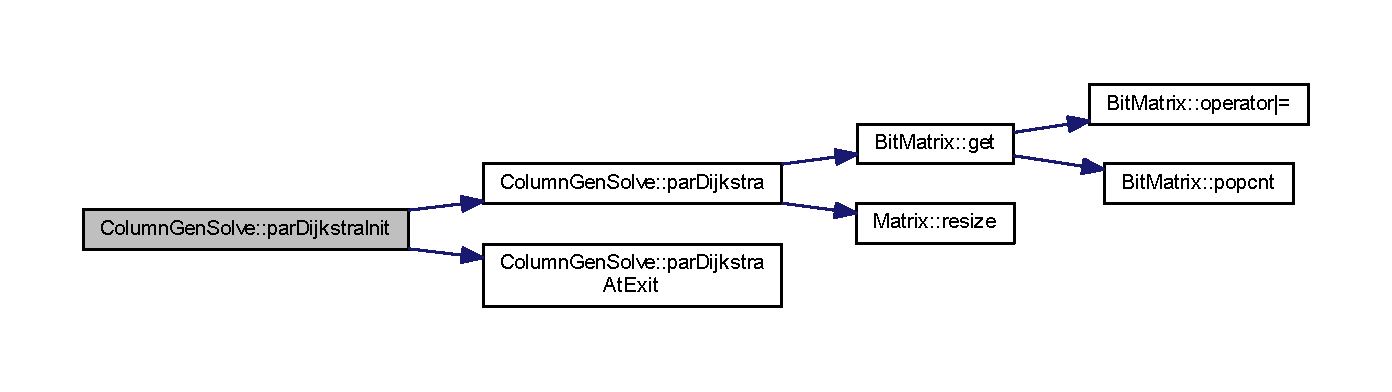
\includegraphics[width=350pt]{classColumnGenSolve_a97e581fdab12a396fd173b030ec26bec_cgraph}
\end{center}
\end{figure}


\index{Column\+Gen\+Solve@{Column\+Gen\+Solve}!push\+Tree\+Set@{push\+Tree\+Set}}
\index{push\+Tree\+Set@{push\+Tree\+Set}!Column\+Gen\+Solve@{Column\+Gen\+Solve}}
\subsubsection[{\texorpdfstring{push\+Tree\+Set(\+Vector$<$ Pair$<$ Tree, G\+R\+B\+Var $>$$>$ \&treeset, Tree \&tree) const }{pushTreeSet(Vector< Pair< Tree, GRBVar >> &treeset, Tree &tree) const }}]{\setlength{\rightskip}{0pt plus 5cm}bool Column\+Gen\+Solve\+::push\+Tree\+Set (
\begin{DoxyParamCaption}
\item[{{\bf Vector}$<$ {\bf Pair}$<$ {\bf Tree}, {\bf G\+R\+B\+Var} $>$$>$ \&}]{treeset, }
\item[{{\bf Tree} \&}]{tree}
\end{DoxyParamCaption}
) const\hspace{0.3cm}{\ttfamily [protected]}}\hypertarget{classColumnGenSolve_a4a1019de523004757e60c023fc92a38d}{}\label{classColumnGenSolve_a4a1019de523004757e60c023fc92a38d}


在文件 Column\+Gen\+Solve.\+cpp 第 1007 行定义.



参考 Tree\+::compute\+Length().



参考自 suggest\+Tree().


\begin{DoxyCode}
1010 \{
1011     \textcolor{keywordflow}{for}(\textcolor{keyword}{const} \textcolor{keyword}{auto} &treeVar: treeset)
1012         \textcolor{keywordflow}{if}(treeVar.first == tree)
1013             \textcolor{keywordflow}{return} \textcolor{keyword}{false};
1014     tree.\hyperlink{classTree_a70810e1d66ffb05f9787ab07c713c104}{computeLength}();
1015     treeset.push\_back(\hyperlink{classPair}{Pair<Tree, GRBVar>}(tree, \hyperlink{classGRBVar}{GRBVar}()));
1016     \textcolor{keywordflow}{return} \textcolor{keyword}{true};
1017 \}
\end{DoxyCode}


函数调用图\+:
\nopagebreak
\begin{figure}[H]
\begin{center}
\leavevmode
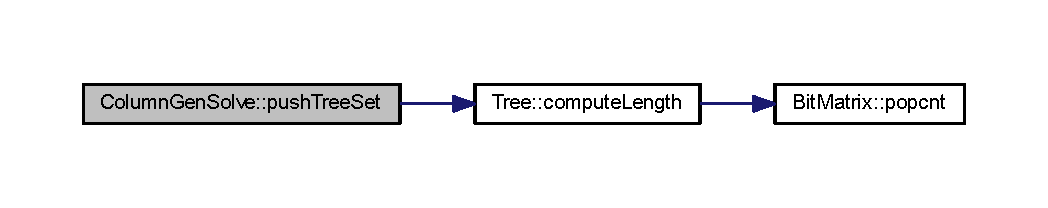
\includegraphics[width=350pt]{classColumnGenSolve_a4a1019de523004757e60c023fc92a38d_cgraph}
\end{center}
\end{figure}




这是这个函数的调用关系图\+:
\nopagebreak
\begin{figure}[H]
\begin{center}
\leavevmode
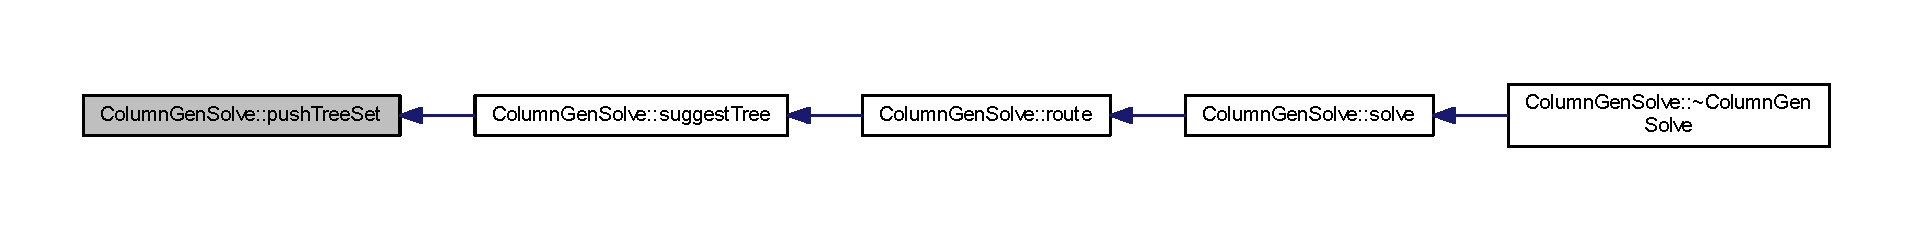
\includegraphics[width=350pt]{classColumnGenSolve_a4a1019de523004757e60c023fc92a38d_icgraph}
\end{center}
\end{figure}


\index{Column\+Gen\+Solve@{Column\+Gen\+Solve}!remove\+Non\+Cuts@{remove\+Non\+Cuts}}
\index{remove\+Non\+Cuts@{remove\+Non\+Cuts}!Column\+Gen\+Solve@{Column\+Gen\+Solve}}
\subsubsection[{\texorpdfstring{remove\+Non\+Cuts(const Matrix$<$ int $>$ \&map, int idx, Bit\+Matrix \&tree, int n, int m, const Matrix$<$ double $>$ $\ast$map\+W=\+N\+U\+L\+L) const }{removeNonCuts(const Matrix< int > &map, int idx, BitMatrix &tree, int n, int m, const Matrix< double > *mapW=NULL) const }}]{\setlength{\rightskip}{0pt plus 5cm}void Column\+Gen\+Solve\+::remove\+Non\+Cuts (
\begin{DoxyParamCaption}
\item[{const {\bf Matrix}$<$ int $>$ \&}]{map, }
\item[{int}]{idx, }
\item[{{\bf Bit\+Matrix} \&}]{tree, }
\item[{int}]{n, }
\item[{int}]{m, }
\item[{const {\bf Matrix}$<$ double $>$ $\ast$}]{mapW = {\ttfamily NULL}}
\end{DoxyParamCaption}
) const\hspace{0.3cm}{\ttfamily [protected]}}\hypertarget{classColumnGenSolve_a6c08d317e692a357d49ee56184a9db22}{}\label{classColumnGenSolve_a6c08d317e692a357d49ee56184a9db22}


在文件 Column\+Gen\+Solve.\+cpp 第 796 行定义.



参考 assert, dfs\+Edge(), dfs\+Father(), dijkstra(), Bit\+Matrix\+::get(), id, points, Bit\+Matrix\+::reset(), Bit\+Matrix\+::set(), sync(), tree\+Get\+Branches(), Point\+::x, y , 以及 Point\+::y.



参考自 suggest\+Tree().


\begin{DoxyCode}
800 \{
801     \textcolor{comment}{// cout << "Begin Removal\(\backslash\)n" << tree;}
802     \textcolor{keyword}{struct }TreeEdge
803     \{
804         \textcolor{keywordtype}{int} s, t;
805         \textcolor{keywordtype}{bool} enabled;
806         \hyperlink{classVector}{Vector<Point>} \hyperlink{classes_8txt_ae368e6252d0add75ea011d5d90db68ed}{points};
807     \};
808     \hyperlink{classVector}{Vector<TreeEdge *>} edges;
809     \hyperlink{classMatrix}{Matrix<int>} \hyperlink{classes_8txt_a7441ef0865bcb3db9b8064dd7375c1ea}{id}; \textcolor{keywordtype}{int} totId = 0;
810     \textcolor{keywordtype}{id}.resize(n, m);
811     \hyperlink{classVector}{Vector<bool>} isKey; isKey.push\_back(\textcolor{keyword}{false});
812     
813     \textcolor{keywordflow}{for}(\textcolor{keywordtype}{int} i = 0; i < n; i++)
814         \textcolor{keywordflow}{for}(\textcolor{keywordtype}{int} j = 0; j < m; j++)
815         \{
816             \textcolor{keywordflow}{if}(!tree.\hyperlink{classBitMatrix_ad19d1045b54ccc8a99d70d38305b4ca6}{get}(i, j))
817                 \textcolor{keywordflow}{continue};
818             \textcolor{keywordtype}{int} deg = 0;
819             \textcolor{keywordflow}{if}(i && tree.\hyperlink{classBitMatrix_ad19d1045b54ccc8a99d70d38305b4ca6}{get}(i - 1, j))
820                 ++deg;
821             \textcolor{keywordflow}{if}(i + 1 < n && tree.\hyperlink{classBitMatrix_ad19d1045b54ccc8a99d70d38305b4ca6}{get}(i + 1, j))
822                 ++deg;
823             \textcolor{keywordflow}{if}(j && tree.\hyperlink{classBitMatrix_ad19d1045b54ccc8a99d70d38305b4ca6}{get}(i, j - 1))
824                 ++deg;
825             \textcolor{keywordflow}{if}(j + 1 < m && tree.\hyperlink{classBitMatrix_ad19d1045b54ccc8a99d70d38305b4ca6}{get}(i, j + 1))
826                 ++deg;
827             \textcolor{keywordflow}{if}(deg == 2 && map[i][j] != idx)
828                 \textcolor{keywordflow}{continue};
829             \textcolor{keywordtype}{id}[i][j] = ++totId;
830             isKey.push\_back(map[i][j] == idx);
831             \textcolor{keywordflow}{if}(i && \textcolor{keywordtype}{id}[i - 1][j])
832             \{
833                 TreeEdge *edge = \textcolor{keyword}{new} TreeEdge;
834                 edge->s = totId; edge->t = \textcolor{keywordtype}{id}[i - 1][j];
835                 edge->enabled = \textcolor{keyword}{false};
836                 edges.push\_back(edge);
837             \}
838             \textcolor{keywordflow}{if}(j && \textcolor{keywordtype}{id}[i][j - 1])
839             \{
840                 TreeEdge *edge = \textcolor{keyword}{new} TreeEdge;
841                 edge->s = totId; edge->t = \textcolor{keywordtype}{id}[i][j - 1];
842                 edge->enabled = \textcolor{keyword}{false};
843                 edges.push\_back(edge);
844             \}
845         \}
846     
847     \textcolor{keywordflow}{for}(\textcolor{keywordtype}{int} i = 0; i < n; i++)
848         \textcolor{keywordflow}{for}(\textcolor{keywordtype}{int} j = 0; j < m; j++)
849         \{
850             \textcolor{keywordflow}{if}(!tree.\hyperlink{classBitMatrix_ad19d1045b54ccc8a99d70d38305b4ca6}{get}(i, j) || \textcolor{keywordtype}{id}[i][j])
851                 \textcolor{keywordflow}{continue};
852             TreeEdge *edge = \textcolor{keyword}{new} TreeEdge;
853             edge->s = 0; edge->t = 0;
854             edge->enabled = \textcolor{keyword}{false};
855             \hyperlink{classColumnGenSolve_a96cbeba5fb978bb67e32b8f42ba161fe}{dfsEdge}(tree, \textcolor{keywordtype}{id}, edge->points, i, j, n, m, edge->s, edge->t);
856             \hyperlink{global_8h_af576bf8ffa22a44e53018c67095ffbf0}{assert}(edge->s); \hyperlink{global_8h_af576bf8ffa22a44e53018c67095ffbf0}{assert}(edge->t);
857             edges.push\_back(edge);
858         \}
859     
860     sort(
861         edges.begin(), edges.end(),
862         [](TreeEdge *x, TreeEdge *\hyperlink{classes_8txt_a52673b1e0cce0104e52dcd12727f211e}{y})
863         \{
864             \textcolor{keywordflow}{return} x->points.size() < \hyperlink{classes_8txt_a52673b1e0cce0104e52dcd12727f211e}{y}->points.size();
865         \}
866     );
867     
868     \hyperlink{classVector}{Vector<int>} father;
869     father.resize(totId + 1);
870     \hyperlink{classVector}{Vector<int>} deg;
871     deg.resize(totId + 1);
872     \hyperlink{classVector}{Vector<Vector<TreeEdge *>}> graphEdges;
873     graphEdges.resize(totId + 1);
874     
875     \textcolor{keywordflow}{for}(\textcolor{keywordtype}{int} i = 1; i <= totId; i++)
876         father[i] = i;
877     \textcolor{keywordflow}{for}(\textcolor{keyword}{auto} edge: edges)
878     \{
879         \textcolor{keywordtype}{int} fatherS = \hyperlink{classColumnGenSolve_af3470aaed4b9d0aa92f27b487b093479}{dfsFather}(father, edge->s);
880         \textcolor{keywordtype}{int} fatherT = \hyperlink{classColumnGenSolve_af3470aaed4b9d0aa92f27b487b093479}{dfsFather}(father, edge->t);
881         \textcolor{keywordflow}{if}(fatherS == fatherT)
882             \textcolor{keywordflow}{continue};
883         father[fatherS] = fatherT;
884         graphEdges[edge->s].push\_back(edge);
885         graphEdges[edge->t].push\_back(edge);
886         ++deg[edge->s];
887         ++deg[edge->t];
888         edge->enabled = \textcolor{keyword}{true};
889     \}
890     
891     \hyperlink{classVector}{Vector<int>} queue;
892     queue.resize(totId + 1);
893     \textcolor{keywordtype}{int} queueHead = 1, queueTail = 0;
894     \hyperlink{classVector}{Vector<bool>} disposed;
895     disposed.resize(totId + 1);
896     \textcolor{keywordflow}{for}(\textcolor{keywordtype}{int} i = 1; i <= totId; i++)
897         \textcolor{keywordflow}{if}(deg[i] == 1 && !isKey[i])
898             queue[++queueTail] = i;
899     \textcolor{keywordflow}{while}(queueHead <= queueTail)
900     \{
901         \textcolor{keywordtype}{int} curId = queue[queueHead++];
902         disposed[curId] = \textcolor{keyword}{true};
903         \textcolor{keywordflow}{for}(\textcolor{keyword}{auto} edge: graphEdges[curId])
904         \{
905             \textcolor{keywordflow}{if}(!edge->enabled)
906                 \textcolor{keywordflow}{continue};
907             \textcolor{keywordtype}{int} otherId = (edge->s ^ edge->t ^ curId);
908             \hyperlink{global_8h_af576bf8ffa22a44e53018c67095ffbf0}{assert}(!disposed[otherId]);
909             \textcolor{keywordflow}{if}((--deg[otherId]) == 1 && !isKey[otherId])
910                 queue[++queueTail] = otherId;
911             edge->enabled = \textcolor{keyword}{false};
912         \}
913     \}
914     
915     \textcolor{keywordflow}{for}(\textcolor{keyword}{auto} edge: edges)
916         \textcolor{keywordflow}{if}(edge->enabled)
917             \textcolor{keywordflow}{for}(\textcolor{keyword}{auto} &point: edge->points)
918                 tree.\hyperlink{classBitMatrix_ad26dd2e93e9d24d70834d6d79e29c81e}{set}(point);
919     
920     \textcolor{keywordflow}{for}(\textcolor{keywordtype}{int} i = 0; i < n; i++)
921         \textcolor{keywordflow}{for}(\textcolor{keywordtype}{int} j = 0; j < m; j++)
922             \textcolor{keywordflow}{if}(\textcolor{keywordtype}{id}[i][j] && disposed[\textcolor{keywordtype}{id}[i][j]])
923                 tree.\hyperlink{classBitMatrix_a0ee870454e6343c3272ab791e45af404}{reset}(i, j);
924     
925     \textcolor{keywordflow}{if}(mapW == NULL)
926         \textcolor{keywordflow}{goto} funcend;
927     
928     \textcolor{comment}{// cout << "optimizing tree\(\backslash\)n";}
929     \textcolor{comment}{// cout << tree;}
930     
931     \textcolor{keywordflow}{for}(\textcolor{keyword}{auto} edge: edges)
932         \textcolor{keywordflow}{if}(edge->enabled)
933         \{
934             \hyperlink{classBitMatrix}{BitMatrix} newTree = tree;
935             \textcolor{keywordflow}{for}(\textcolor{keyword}{auto} point: edge->points)
936                 newTree.\hyperlink{classBitMatrix_a0ee870454e6343c3272ab791e45af404}{reset}(point);
937             \hyperlink{classVector}{Vector<BitMatrix>} branches = \hyperlink{classColumnGenSolve_acbcc78e94e4a6e59ceb7da2357ddb87a}{treeGetBranches}(newTree, n, m);
938             \textcolor{comment}{// cout << "branchsize " << (int) branches.size() << '\(\backslash\)n';}
939             \textcolor{keywordflow}{if}((\textcolor{keywordtype}{int}) branches.size() != 2) \textcolor{keywordflow}{continue};
940             \hyperlink{classMatrix}{Matrix<Pair<double, Point>}> dijResult;
941             \hyperlink{classColumnGenSolve_a71007959556061091171c03da6197f34}{dijkstra}(branches[0], *mapW, n, m, dijResult);
942             \hyperlink{classColumnGenSolve_ab976cab8582808218110d86252177f88}{sync}();
943             \hyperlink{classPoint}{Point} bestPoint1(-1, -1); \textcolor{keywordtype}{double} dist = 1e30;
944             \textcolor{keywordflow}{for}(\textcolor{keywordtype}{int} i = 0; i < n; i++)
945                 \textcolor{keywordflow}{for}(\textcolor{keywordtype}{int} j = 0; j < m; j++)
946                     \textcolor{keywordflow}{if}(branches[1].\textcolor{keyword}{get}(i, j) && dijResult[i][j].first < dist)
947                     \{
948                         dist = dijResult[i][j].first;
949                         bestPoint1.x = i; bestPoint1.y = j;
950                     \}
951             \textcolor{comment}{// cout << "dist " << dist << '\(\backslash\)n';}
952             \textcolor{keywordflow}{for}(\textcolor{keyword}{auto} point: edge->points)
953                 dist -= (*mapW)[point];
954             \textcolor{comment}{// cout << "dist " << dist << '\(\backslash\)n';}
955             \textcolor{keyword}{static} \textcolor{keywordtype}{int} a = 0;
956             \textcolor{keyword}{static} \textcolor{keywordtype}{int} b = 0;
957             a += (int) (dist >= 0); b++;
958             \textcolor{comment}{// cout << "q " << a << "/" << b << "\(\backslash\)n";}
959             \textcolor{comment}{// cout.flush();}
960             \textcolor{keywordflow}{if}(dist >= 0)
961                 \textcolor{keywordflow}{continue};
962             \textcolor{keywordflow}{while}(bestPoint1 != \hyperlink{classPoint}{Point}(-1, -1))
963             \{
964                 newTree.\hyperlink{classBitMatrix_ad26dd2e93e9d24d70834d6d79e29c81e}{set}(bestPoint1);
965                 bestPoint1 = dijResult[bestPoint1].second;
966             \}
967             \hyperlink{classColumnGenSolve_a6c08d317e692a357d49ee56184a9db22}{removeNonCuts}(map, idx, newTree, n, m, mapW);
968             tree = newTree;
969             \textcolor{keywordflow}{goto} funcend;
970         \}
971     
972     funcend:;
973     \textcolor{keywordflow}{for}(\textcolor{keyword}{auto} edge: edges)
974         \textcolor{keyword}{delete} edge;
975     
976     \textcolor{comment}{// if(mapW != NULL)}
977     \textcolor{comment}{// \{}
978         \textcolor{comment}{// cout << "optimize finished\(\backslash\)n";}
979         \textcolor{comment}{// cout << tree;}
980     \textcolor{comment}{// \}}
981 
982     \textcolor{comment}{// cout << "End Removal\(\backslash\)n" << tree;}
983 \}
\end{DoxyCode}


函数调用图\+:
\nopagebreak
\begin{figure}[H]
\begin{center}
\leavevmode
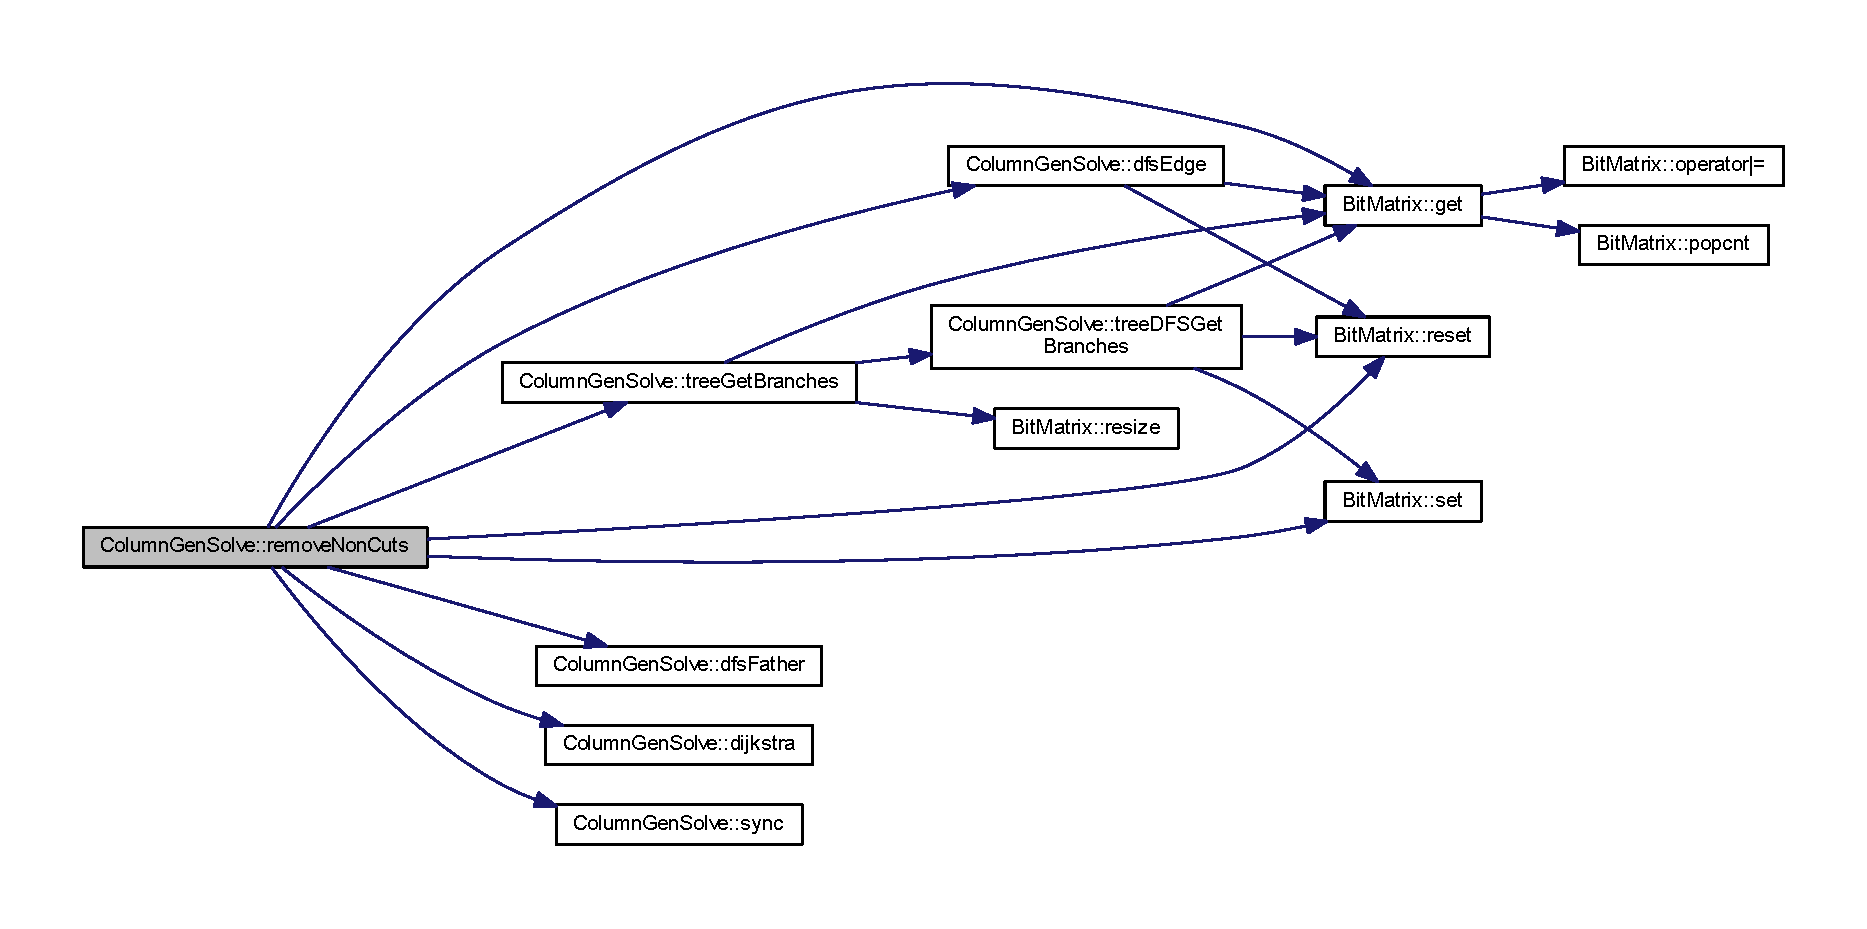
\includegraphics[width=350pt]{classColumnGenSolve_a6c08d317e692a357d49ee56184a9db22_cgraph}
\end{center}
\end{figure}




这是这个函数的调用关系图\+:
\nopagebreak
\begin{figure}[H]
\begin{center}
\leavevmode
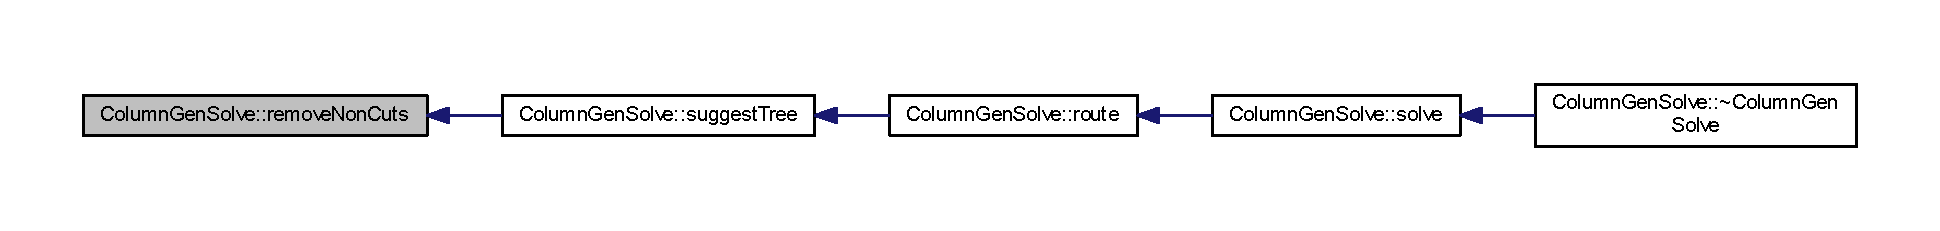
\includegraphics[width=350pt]{classColumnGenSolve_a6c08d317e692a357d49ee56184a9db22_icgraph}
\end{center}
\end{figure}


\index{Column\+Gen\+Solve@{Column\+Gen\+Solve}!remove\+Non\+Cuts@{remove\+Non\+Cuts}}
\index{remove\+Non\+Cuts@{remove\+Non\+Cuts}!Column\+Gen\+Solve@{Column\+Gen\+Solve}}
\subsubsection[{\texorpdfstring{remove\+Non\+Cuts(\+Matrix$<$ bool $>$ \&visited, const Matrix$<$ int $>$ \&map, int idx, const Matrix$<$ double $>$ \&map\+W, Bit\+Matrix \&tree, int n, int m) const }{removeNonCuts(Matrix< bool > &visited, const Matrix< int > &map, int idx, const Matrix< double > &mapW, BitMatrix &tree, int n, int m) const }}]{\setlength{\rightskip}{0pt plus 5cm}double Column\+Gen\+Solve\+::remove\+Non\+Cuts (
\begin{DoxyParamCaption}
\item[{{\bf Matrix}$<$ bool $>$ \&}]{visited, }
\item[{const {\bf Matrix}$<$ int $>$ \&}]{map, }
\item[{int}]{idx, }
\item[{const {\bf Matrix}$<$ double $>$ \&}]{mapW, }
\item[{{\bf Bit\+Matrix} \&}]{tree, }
\item[{int}]{n, }
\item[{int}]{m}
\end{DoxyParamCaption}
) const\hspace{0.3cm}{\ttfamily [protected]}}\hypertarget{classColumnGenSolve_ad5a36333d83b1a1803eb582c9a0a9941}{}\label{classColumnGenSolve_ad5a36333d83b1a1803eb582c9a0a9941}


在文件 Column\+Gen\+Solve.\+cpp 第 985 行定义.



参考 Bit\+Matrix\+::get(), Bit\+Matrix\+::reset() , 以及 tree\+Is\+Cut().


\begin{DoxyCode}
989 \{
990     \textcolor{keywordtype}{double} ans = 0;
991     begin:
992     \textcolor{keywordflow}{for}(\textcolor{keywordtype}{int} i = 0; i < n; i++)
993         \textcolor{keywordflow}{for}(\textcolor{keywordtype}{int} j = 0; j < m; j++)
994             \textcolor{keywordflow}{if}(
995                 tree.\hyperlink{classBitMatrix_ad19d1045b54ccc8a99d70d38305b4ca6}{get}(i, j) && map[i][j] != idx
996                 && !\hyperlink{classColumnGenSolve_ae971ef7c0098fd33bea1701fbfe92f4f}{treeIsCut}(tree, i, j, n, m)
997             )
998             \{
999                 visited[i][j] = 1;
1000                 tree.\hyperlink{classBitMatrix_a0ee870454e6343c3272ab791e45af404}{reset}(i, j);
1001                 ans += mapW[i][j];
1002                 \textcolor{keywordflow}{goto} begin;
1003             \}
1004     \textcolor{keywordflow}{return} ans;
1005 \}
\end{DoxyCode}


函数调用图\+:
\nopagebreak
\begin{figure}[H]
\begin{center}
\leavevmode
\includegraphics[width=350pt]{classColumnGenSolve_ad5a36333d83b1a1803eb582c9a0a9941_cgraph}
\end{center}
\end{figure}


\index{Column\+Gen\+Solve@{Column\+Gen\+Solve}!route@{route}}
\index{route@{route}!Column\+Gen\+Solve@{Column\+Gen\+Solve}}
\subsubsection[{\texorpdfstring{route(int tim) const }{route(int tim) const }}]{\setlength{\rightskip}{0pt plus 5cm}{\bf Vector}$<$ {\bf Tree} $\ast$ $>$ Column\+Gen\+Solve\+::route (
\begin{DoxyParamCaption}
\item[{int}]{tim}
\end{DoxyParamCaption}
) const\hspace{0.3cm}{\ttfamily [protected]}}\hypertarget{classColumnGenSolve_af97cd5f1c4a7305b72e46971fdb85002}{}\label{classColumnGenSolve_af97cd5f1c4a7305b72e46971fdb85002}


在文件 Column\+Gen\+Solve.\+cpp 第 106 行定义.



参考 Solver\+::board, Solution\+::board, board, Solution\+::compute\+Map(), G\+R\+B\+\_\+\+Double\+Attr\+\_\+X, Board\+::height, M, Board\+::map, map, points, Matrix$<$ T $>$\+::resize(), solution, solve\+L\+P(), Solve\+Strategy\+::solver, suggest\+Tree(), Board\+::terminal\+Sets, Solution\+::trees , 以及 Board\+::width.



参考自 solve().


\begin{DoxyCode}
107 \{
108     \textcolor{comment}{// Open a console for output}
109     \hyperlink{global_8h_a7ec5bb64a5a7c56f5600caebf1ac2b7e}{OFStream} con(\textcolor{stringliteral}{"con"});
110     \textcolor{keyword}{auto} clkStart = clock();
111     
112     \textcolor{comment}{// Constant definition}
113     \textcolor{keyword}{const} \hyperlink{classBoard}{Board} *\hyperlink{classes_8txt_ab2104b75e0965a7c5fc13208045d9b59}{board} = \hyperlink{classSolveStrategy_a94d43c47305176d0d3858697d3410443}{solver}->\hyperlink{classSolver_a8966a22c2f247addc8ce453d119bc54e}{board};
114     \textcolor{keyword}{const} \hyperlink{classVector}{Vector<TerminalSet *>} &termsets = board->
      \hyperlink{classBoard_a6683a9c042af7113f55c5bc1b9656b69}{terminalSets};
115     \textcolor{keyword}{const} \hyperlink{classMatrix}{Matrix<int>} &\hyperlink{classes_8txt_a0a12e395730487ab04f7f11cbc4d2132}{map} = board->\hyperlink{classBoard_a191ff45df9151b8fee0c32877f582165}{map};
116     \textcolor{keyword}{const} \textcolor{keywordtype}{int} t = termsets.size() - 1;
117     \textcolor{keyword}{const} \textcolor{keywordtype}{int} n = board->\hyperlink{classBoard_aa0cb8de0254520dc08dab5796643c8e5}{height};
118     \textcolor{keyword}{const} \textcolor{keywordtype}{int} m = board->\hyperlink{classBoard_a90a8efaa4736af25511ac948bdd27d6c}{width};
119     \textcolor{keywordflow}{if}(n * m >= 1250)
120         cout << \textcolor{stringliteral}{"solving subproblem "} << n << \textcolor{stringliteral}{" * "} << m << \textcolor{stringliteral}{"\(\backslash\)n"};
121     
122     \textcolor{comment}{// Two useful Vectors}
123     \textcolor{comment}{/*}
124 \textcolor{comment}{    Vector<Point> allPoints;}
125 \textcolor{comment}{    for(int i = 0; i < n; i++)}
126 \textcolor{comment}{        for(int j = 0; j < m; j++)}
127 \textcolor{comment}{            allPoints.push\_back(Point(i, j));}
128 \textcolor{comment}{    */}
129     
130     \hyperlink{classMatrix}{Matrix<double>} all1;
131     all1.\hyperlink{classMatrix_a15ce96c8af4c7a982c2c10b96f29cea1}{resize}(n, m);
132     \textcolor{keywordflow}{for}(\textcolor{keywordtype}{int} i = 0; i < n; i++)
133         \textcolor{keywordflow}{for}(\textcolor{keywordtype}{int} j = 0; j < m; j++)
134             all1[i][j] = 1;
135     
136     \textcolor{comment}{// The tree set, initially empty}
137     \hyperlink{classVector}{Vector<Vector<Pair<Tree, GRBVar>}>> treesets;
138     
139     \textcolor{keywordflow}{for}(\textcolor{keywordtype}{int} idx = 1; idx <= t; idx++)
140     \{
141         \textcolor{comment}{// Current tree set}
142         \hyperlink{classVector}{Vector<Pair<Tree, GRBVar>}> vec;
143         \textcolor{comment}{/*}
144 \textcolor{comment}{        // If "Precise", all points can be joint}
145 \textcolor{comment}{        if(this->m\_mode == "Precise")}
146 \textcolor{comment}{            for(auto joint: allPoints)\{}
147 \textcolor{comment}{                // Call Dijkstra}
148 \textcolor{comment}{                Matrix<bool> base;}
149 \textcolor{comment}{                base.resize(n, m);}
150 \textcolor{comment}{                base[joint.first][joint.second] = 1;}
151 \textcolor{comment}{                Matrix<Pair<double, Matrix<bool>>> dijRes}
152 \textcolor{comment}{                    = this->dijkstra(base, all1, n, m);}
153 \textcolor{comment}{                // Generate a tree with Dijkstra}
154 \textcolor{comment}{                // result}
155 \textcolor{comment}{                Tree tree(this->m\_board, idx);}
156 \textcolor{comment}{                tree.m\_tree[joint.first][joint.second] = 1;}
157 \textcolor{comment}{                for(auto term: termsets[idx])}
158 \textcolor{comment}{                \{}
159 \textcolor{comment}{                    tree.m\_tree[term.first][term.second] = 1;}
160 \textcolor{comment}{                    for(int i = 0; i < n; i++)}
161 \textcolor{comment}{                        for(int j = 0; j < m; j++)}
162 \textcolor{comment}{                            if(dijRes[term].second[i][j])}
163 \textcolor{comment}{                                tree.m\_tree[i][j] = 1;}
164 \textcolor{comment}{                \}}
165 \textcolor{comment}{                this->removeNonCuts(}
166 \textcolor{comment}{                    map, idx, tree.m\_tree, n, m, joint.first, joint.second}
167 \textcolor{comment}{                );}
168 \textcolor{comment}{                // Add the tree to the set}
169 \textcolor{comment}{                vec.push\_back(tree);}
170 \textcolor{comment}{            \}}
171 \textcolor{comment}{        */}
172         \textcolor{comment}{// Add the set to the set list}
173         treesets.push\_back(vec);
174     \}
175     
176     \textcolor{comment}{// Answer history}
177     \hyperlink{classVector}{Vector<double>} tarAns;
178     \textcolor{keywordflow}{for}(\textcolor{keywordtype}{int} T = 0;; T++)\{
179         \textcolor{comment}{// cout << "LP " << T << endl;}
180         \textcolor{comment}{// Solve the integer (binary) programming problem}
181         \textcolor{keywordtype}{double} curAns = \hyperlink{classColumnGenSolve_aadb23efa531a3eb68651ba11f4d36c81}{solveLP}(treesets, 1);
182         tarAns.push\_back(curAns);
183         
184         \textcolor{comment}{// Construct current best answer}
185         \hyperlink{classVector}{Vector<Tree *>} ans;
186         \textcolor{keywordflow}{for}(\textcolor{keyword}{const} \textcolor{keyword}{auto} &treeset: treesets)
187         \{
188             \textcolor{keywordflow}{for}(\textcolor{keyword}{const} \textcolor{keyword}{auto} &treeVar: treeset)
189                 \textcolor{keywordflow}{if}(treeVar.second.get(\hyperlink{gurobi__c_09_09_8h_a2f43cc28447ce1778973a1f7961e8180a88afa2b5caf4dd5e8b44785752f6940a}{GRB\_DoubleAttr\_X}) > 0.5)
190                 \{
191                     ans.push\_back(\textcolor{keyword}{new} \hyperlink{classTree}{Tree}(treeVar.first));
192                     \textcolor{keywordflow}{goto} found;
193                 \}
194             ans.push\_back(NULL);
195             found:;
196         \}
197         
198         \textcolor{comment}{// if(T >= 3)}
199             \textcolor{comment}{// return ans;}
200         \textcolor{comment}{// output(ans, con);}
201         \textcolor{comment}{// output(ans, cout);}
202         
203         \textcolor{keywordtype}{bool} updated = \textcolor{keyword}{false};
204         \textcolor{comment}{// Build weight map for unrouted set}
205         \hyperlink{classMatrix}{Matrix<double>} mapObs;
206         mapObs.\hyperlink{classMatrix_a15ce96c8af4c7a982c2c10b96f29cea1}{resize}(n, m);
207         \textcolor{keywordflow}{for}(\textcolor{keywordtype}{int} i = 0; i < n; i++)
208             \textcolor{keywordflow}{for}(\textcolor{keywordtype}{int} j = 0; j < m; j++)
209                 \textcolor{keywordflow}{if}(map[i][j] == -1)
210                     mapObs[i][j] = \hyperlink{classColumnGenSolve_ac5abb4d6dfd291b01af6ea006b5f9f5d}{M};
211                 \textcolor{keywordflow}{else}
212                     mapObs[i][j] = 1;
213         
214         \textcolor{keywordflow}{for}(\textcolor{keywordtype}{int} idx = 1; idx <= t; idx++)
215             \textcolor{keywordflow}{if}(ans[idx - 1])
216                 \textcolor{keywordflow}{for}(\textcolor{keywordtype}{int} i = 0; i < n; i++)
217                     \textcolor{keywordflow}{for}(\textcolor{keywordtype}{int} j = 0; j < m; j++)
218                         \textcolor{keywordflow}{if}(ans[idx - 1]->map.get(i, j))
219                             mapObs[i][j] = \hyperlink{classColumnGenSolve_ac5abb4d6dfd291b01af6ea006b5f9f5d}{M};
220         \textcolor{comment}{// Try to generate from each set}
221         \textcolor{keywordflow}{for}(\textcolor{keywordtype}{int} idx = 1; idx <= t; idx++)
222         \{
223             \textcolor{keywordflow}{if}(termsets[idx]->\hyperlink{classes_8txt_ae368e6252d0add75ea011d5d90db68ed}{points}.empty())
224                 \textcolor{keywordflow}{continue};
225             \textcolor{keywordflow}{if}(!ans[idx - 1])\{
226                 \textcolor{comment}{// If unrouted, try to generate from the map above}
227                 \textcolor{keywordflow}{if}(\hyperlink{classColumnGenSolve_a4ec729b2184612495e657f7ec2d644fa}{suggestTree}(termsets, treesets, mapObs, n, m, idx))
228                     updated = \textcolor{keyword}{true};
229             \}\textcolor{keywordflow}{else}\{
230                 \textcolor{comment}{// If routed}
231                 \{
232                     \textcolor{comment}{// Try to reroute current set}
233                     \hyperlink{classMatrix}{Matrix<double>} mapObs2 = mapObs;
234                     \textcolor{keywordflow}{for}(\textcolor{keywordtype}{int} i = 0; i < n; i++)
235                         \textcolor{keywordflow}{for}(\textcolor{keywordtype}{int} j = 0; j < m; j++)
236                             \textcolor{keywordflow}{if}(
237                                 mapObs2[i][j] >= \hyperlink{classColumnGenSolve_ac5abb4d6dfd291b01af6ea006b5f9f5d}{M} / 2
238                                 && ans[idx - 1]->map.get(i, j)
239                             )
240                                 mapObs2[i][j] = 1;
241                     \textcolor{keywordflow}{if}(\hyperlink{classColumnGenSolve_a4ec729b2184612495e657f7ec2d644fa}{suggestTree}(termsets, treesets, mapObs2, n, m, idx))
242                         updated = \textcolor{keyword}{true};
243                 \}
244                 \{
245                     \textcolor{comment}{/*}
246 \textcolor{comment}{                        Try to reroute current set and try to route another tree}
247 \textcolor{comment}{                        rather than current tree}
248 \textcolor{comment}{                    */}
249                     \hyperlink{classMatrix}{Matrix<double>} mapObs2 = mapObs;
250                     \textcolor{keywordflow}{for}(\textcolor{keywordtype}{int} i = 0; i < n; i++)
251                         \textcolor{keywordflow}{for}(\textcolor{keywordtype}{int} j = 0; j < m; j++)
252                             \textcolor{keywordflow}{if}(
253                                 mapObs2[i][j] >= \hyperlink{classColumnGenSolve_ac5abb4d6dfd291b01af6ea006b5f9f5d}{M} / 2 &&
254                                 !ans[idx - 1]->map.get(i, j)
255                             ) mapObs2[i][j] = \hyperlink{classColumnGenSolve_ac5abb4d6dfd291b01af6ea006b5f9f5d}{M} * \hyperlink{classColumnGenSolve_ac5abb4d6dfd291b01af6ea006b5f9f5d}{M};
256                     \textcolor{keywordflow}{if}(\hyperlink{classColumnGenSolve_a4ec729b2184612495e657f7ec2d644fa}{suggestTree}(termsets, treesets, mapObs2, n, m, idx))
257                         updated = \textcolor{keyword}{true};
258                 \}
259                 \{
260                     \textcolor{comment}{/*}
261 \textcolor{comment}{                        Try to solve integer programming without current set and}
262 \textcolor{comment}{                        try to avoid overlap between current tree and the}
263 \textcolor{comment}{                        solution above}
264 \textcolor{comment}{                    */}
265                     \hyperlink{classColumnGenSolve_aadb23efa531a3eb68651ba11f4d36c81}{solveLP}(treesets, 1, NULL, NULL, idx);
266                     
267                     \hyperlink{classVector}{Vector<Tree *>} tmpAns;
268                     
269                     \textcolor{keywordflow}{for}(\textcolor{keywordtype}{int} i = 0; i < t; i++)
270                         \textcolor{keywordflow}{if}(i != idx - 1)
271                         \{
272                             \textcolor{keywordflow}{for}(\textcolor{keyword}{const} \textcolor{keyword}{auto} &treeVar: treesets[i])
273                                 \textcolor{keywordflow}{if}(treeVar.second.get(\hyperlink{gurobi__c_09_09_8h_a2f43cc28447ce1778973a1f7961e8180a88afa2b5caf4dd5e8b44785752f6940a}{GRB\_DoubleAttr\_X}) > 0.5)
274                                 \{
275                                     tmpAns.push\_back(\textcolor{keyword}{new} \hyperlink{classTree}{Tree}(treeVar.first));
276                                     \textcolor{keywordflow}{goto} found2;
277                                 \}
278                             tmpAns.push\_back(NULL);
279                             found2:;
280                         \}
281                         \textcolor{keywordflow}{else}
282                             tmpAns.push\_back(NULL);
283                     
284                     \textcolor{comment}{// OK, let's construct weight map}
285                     \hyperlink{classMatrix}{Matrix<double>} mapObs2;
286                     mapObs2.\hyperlink{classMatrix_a15ce96c8af4c7a982c2c10b96f29cea1}{resize}(n, m);
287                     \textcolor{keywordflow}{for}(\textcolor{keywordtype}{int} i = 0; i < n; i++)
288                         \textcolor{keywordflow}{for}(\textcolor{keywordtype}{int} j = 0; j < m; j++)
289                             \textcolor{keywordflow}{if}(map[i][j] == -1)
290                                 mapObs2[i][j] = \hyperlink{classColumnGenSolve_ac5abb4d6dfd291b01af6ea006b5f9f5d}{M} * \hyperlink{classColumnGenSolve_ac5abb4d6dfd291b01af6ea006b5f9f5d}{M};
291                             \textcolor{keywordflow}{else}
292                                 mapObs2[i][j] = 1;
293                     
294                     \textcolor{keywordflow}{for}(\textcolor{keywordtype}{int} nidx = 1; nidx <= t; nidx++)
295                         \textcolor{keywordflow}{if}(tmpAns[nidx - 1])
296                             \textcolor{keywordflow}{for}(\textcolor{keywordtype}{int} i = 0; i < n; i++)
297                                 \textcolor{keywordflow}{for}(\textcolor{keywordtype}{int} j = 0; j < m; j++)
298                                     \textcolor{keywordflow}{if}(tmpAns[nidx - 1]->map.get(i, j))
299                                         mapObs2[i][j] = M;
300                     
301                     \textcolor{keywordflow}{if}(\hyperlink{classColumnGenSolve_a4ec729b2184612495e657f7ec2d644fa}{suggestTree}(termsets, treesets, mapObs2, n, m, idx))
302                         updated = \textcolor{keyword}{true};
303                     
304                     \textcolor{comment}{// clean up}
305                     \textcolor{keywordflow}{for}(\textcolor{keyword}{auto} tree: tmpAns)
306                         \textcolor{keyword}{delete} tree;
307                 \}
308             \}
309         \}
310         
311         \textcolor{keyword}{auto} clkNow = clock();
312         \textcolor{comment}{/*if((int) ((clkNow - clkStart) / CLOCKS\_PER\_SEC) > tim)}
313 \textcolor{comment}{        \{}
314 \textcolor{comment}{            con << "time up, aborting\(\backslash\)n";}
315 \textcolor{comment}{            con << (int) ((clkNow - clkStart) / CLOCKS\_PER\_SEC)}
316 \textcolor{comment}{                << " seconds passed\(\backslash\)n";}
317 \textcolor{comment}{            //return ans;}
318 \textcolor{comment}{        \}*/}
319         
320         \textcolor{comment}{// If solution didn't improve recently,}
321         \textcolor{comment}{// cut!}
322         \textcolor{keywordflow}{if}(T >= 1 && fabs(tarAns[T - 1] - tarAns[T]) < 0.5)
323             \textcolor{keywordflow}{return} ans;
324         
325         \textcolor{comment}{// Output current colution info}
326         \textcolor{keywordflow}{if}(n * m >= 20000)
327         \{
328             cout << \textcolor{stringliteral}{"iteration "} << T << \textcolor{stringliteral}{"\(\backslash\)n"};
329             cout << \textcolor{stringliteral}{"current time: "}
330                 << (int) ((clkNow - clkStart) / CLOCKS\_PER\_SEC) << \textcolor{stringliteral}{" seconds\(\backslash\)n"};
331             cout << \textcolor{stringliteral}{"curAns "} << curAns << endl;
332             cout << \textcolor{stringliteral}{"column sizes:\(\backslash\)n"};
333             \textcolor{keywordflow}{for}(\textcolor{keyword}{const} \textcolor{keyword}{auto} &treeset: treesets)
334                 cout << treeset.size() << \textcolor{stringliteral}{" "};
335             cout << \textcolor{stringliteral}{"\(\backslash\)n"};
336             cout.flush();
337             \textcolor{keywordflow}{if}(n * m >= 80000)
338             \{
339                 \hyperlink{classSolution}{Solution} \hyperlink{classes_8txt_aa43d5190bbc491d9c9134146e01a248e}{solution};
340                 solution.\hyperlink{classSolution_ac4f88cd3aa0713e8900f33eb9f1f15bf}{board} = \hyperlink{classSolveStrategy_a94d43c47305176d0d3858697d3410443}{solver}->\hyperlink{classSolver_a8966a22c2f247addc8ce453d119bc54e}{board};
341                 solution.\hyperlink{classSolution_a554205b5c578add14d2d7836042215d8}{trees}.push\_back(NULL);
342                 \textcolor{keywordflow}{for}(\textcolor{keyword}{auto} tree: ans)
343                     \textcolor{keywordflow}{if}(tree)
344                         solution.\hyperlink{classSolution_a554205b5c578add14d2d7836042215d8}{trees}.push\_back(\textcolor{keyword}{new} \hyperlink{classTree}{Tree}(*tree));
345                     \textcolor{keywordflow}{else}
346                         solution.\hyperlink{classSolution_a554205b5c578add14d2d7836042215d8}{trees}.push\_back(NULL);
347                 solution.\hyperlink{classSolution_a45e5ef985917b725347a0742fe887400}{computeMap}();
348                 con << \hyperlink{classes_8txt_aa43d5190bbc491d9c9134146e01a248e}{solution};
349                 con.flush();
350             \}
351         \}
352         \textcolor{comment}{/*}
353 \textcolor{comment}{        // Solve LP}
354 \textcolor{comment}{        Matrix<double> mapPi;}
355 \textcolor{comment}{        Vector<double> vecLambda;}
356 \textcolor{comment}{        }
357 \textcolor{comment}{        tarAns.push\_back(solveLP(treesets, 0, &mapPi, &vecLambda));}
358 \textcolor{comment}{        }
359 \textcolor{comment}{        // Only try to expand when Dijkstra cannot find any solution}
360 \textcolor{comment}{        if(!updated)}
361 \textcolor{comment}{            for(int i = 0; i < t; i++)\{}
362 \textcolor{comment}{                if(termsets[i + 1]->points.empty())}
363 \textcolor{comment}{                    continue;}
364 \textcolor{comment}{                int oldSize = treesets[i].size();}
365 \textcolor{comment}{                sort(}
366 \textcolor{comment}{                    treesets[i].begin(), treesets[i].end(),}
367 \textcolor{comment}{                    [](const Pair<Tree, GRBVar> &l, const Pair<Tree, GRBVar> &r)}
368 \textcolor{comment}{                    \{}
369 \textcolor{comment}{                        return l.second.get(GRB\_DoubleAttr\_X)}
370 \textcolor{comment}{                            > r.second.get(GRB\_DoubleAttr\_X);}
371 \textcolor{comment}{                    \}}
372 \textcolor{comment}{                );}
373 \textcolor{comment}{                try}
374 \textcolor{comment}{                \{}
375 \textcolor{comment}{                    // int r = 10;}
376 \textcolor{comment}{                    // expand(mapPi, vecLambda[i], treesets[i], n, m, i + 1, r);}
377 \textcolor{comment}{                \}}
378 \textcolor{comment}{                catch(expandFinished)\{\}}
379 \textcolor{comment}{                if((int) treesets[i].size() != oldSize)}
380 \textcolor{comment}{                    updated = true;}
381 \textcolor{comment}{            \}}
382 \textcolor{comment}{            }
383 \textcolor{comment}{        */}
384         
385         \textcolor{comment}{// Still cannot generate, cut}
386         \textcolor{keywordflow}{if}(!updated)
387             \textcolor{keywordflow}{return} ans;
388         
389         \textcolor{comment}{// Clean up}
390         \textcolor{keywordflow}{for}(\textcolor{keyword}{auto} tree: ans)
391             \textcolor{keyword}{delete} tree;
392     \}
393 \}
\end{DoxyCode}


函数调用图\+:
\nopagebreak
\begin{figure}[H]
\begin{center}
\leavevmode
\includegraphics[width=350pt]{classColumnGenSolve_af97cd5f1c4a7305b72e46971fdb85002_cgraph}
\end{center}
\end{figure}




这是这个函数的调用关系图\+:
\nopagebreak
\begin{figure}[H]
\begin{center}
\leavevmode
\includegraphics[width=350pt]{classColumnGenSolve_af97cd5f1c4a7305b72e46971fdb85002_icgraph}
\end{center}
\end{figure}


\index{Column\+Gen\+Solve@{Column\+Gen\+Solve}!solve@{solve}}
\index{solve@{solve}!Column\+Gen\+Solve@{Column\+Gen\+Solve}}
\subsubsection[{\texorpdfstring{solve() const }{solve() const }}]{\setlength{\rightskip}{0pt plus 5cm}{\bf Solution} Column\+Gen\+Solve\+::solve (
\begin{DoxyParamCaption}
{}
\end{DoxyParamCaption}
) const\hspace{0.3cm}{\ttfamily [virtual]}}\hypertarget{classColumnGenSolve_aad7c316627e7ea6de4138db1a33e66ee}{}\label{classColumnGenSolve_aad7c316627e7ea6de4138db1a33e66ee}


实现了 \hyperlink{classSolveStrategy_ad3c3800be3e04570b466c3d8d054c500}{Solve\+Strategy}.



在文件 Column\+Gen\+Solve.\+cpp 第 1087 行定义.



参考 Solver\+::board, Solution\+::board, Solution\+::compute\+Map(), Board\+::height, route(), solution, Solve\+Strategy\+::solver, Solution\+::trees , 以及 Board\+::width.



参考自 $\sim$\+Column\+Gen\+Solve().


\begin{DoxyCode}
1088 \{
1089     \hyperlink{classSolution}{Solution} \hyperlink{classes_8txt_aa43d5190bbc491d9c9134146e01a248e}{solution};
1090     solution.\hyperlink{classSolution_ac4f88cd3aa0713e8900f33eb9f1f15bf}{board} = \hyperlink{classSolveStrategy_a94d43c47305176d0d3858697d3410443}{solver}->\hyperlink{classSolver_a8966a22c2f247addc8ce453d119bc54e}{board};
1091     \hyperlink{classVector}{Vector<Tree *>} res = \hyperlink{classColumnGenSolve_af97cd5f1c4a7305b72e46971fdb85002}{route}(\hyperlink{classSolveStrategy_a94d43c47305176d0d3858697d3410443}{solver}->\hyperlink{classSolver_a8966a22c2f247addc8ce453d119bc54e}{board}->
      \hyperlink{classBoard_a90a8efaa4736af25511ac948bdd27d6c}{width} * \hyperlink{classSolveStrategy_a94d43c47305176d0d3858697d3410443}{solver}->\hyperlink{classSolver_a8966a22c2f247addc8ce453d119bc54e}{board}->\hyperlink{classBoard_aa0cb8de0254520dc08dab5796643c8e5}{height} / 100 + 1);
1092     solution.\hyperlink{classSolution_a554205b5c578add14d2d7836042215d8}{trees}.push\_back(NULL);
1093     \textcolor{keywordflow}{for}(\textcolor{keyword}{auto} tree: res)
1094         solution.\hyperlink{classSolution_a554205b5c578add14d2d7836042215d8}{trees}.push\_back(tree);
1095     solution.\hyperlink{classSolution_a45e5ef985917b725347a0742fe887400}{computeMap}();
1096     \textcolor{keywordflow}{return} \hyperlink{classes_8txt_aa43d5190bbc491d9c9134146e01a248e}{solution};
1097 \}
\end{DoxyCode}


函数调用图\+:
\nopagebreak
\begin{figure}[H]
\begin{center}
\leavevmode
\includegraphics[width=350pt]{classColumnGenSolve_aad7c316627e7ea6de4138db1a33e66ee_cgraph}
\end{center}
\end{figure}




这是这个函数的调用关系图\+:
\nopagebreak
\begin{figure}[H]
\begin{center}
\leavevmode
\includegraphics[width=350pt]{classColumnGenSolve_aad7c316627e7ea6de4138db1a33e66ee_icgraph}
\end{center}
\end{figure}


\index{Column\+Gen\+Solve@{Column\+Gen\+Solve}!solve\+LP@{solve\+LP}}
\index{solve\+LP@{solve\+LP}!Column\+Gen\+Solve@{Column\+Gen\+Solve}}
\subsubsection[{\texorpdfstring{solve\+L\+P(\+Vector$<$ Vector$<$ Pair$<$ Tree, G\+R\+B\+Var $>$$>$$>$ \&treesets, int mode, Matrix$<$ double $>$ $\ast$map\+Pi=\+N\+U\+L\+L, Vector$<$ double $>$ $\ast$vec\+Lambda=\+N\+U\+L\+L, int ignore\+Idx=-\/1) const }{solveLP(Vector< Vector< Pair< Tree, GRBVar >>> &treesets, int mode, Matrix< double > *mapPi=NULL, Vector< double > *vecLambda=NULL, int ignoreIdx=-1) const }}]{\setlength{\rightskip}{0pt plus 5cm}double Column\+Gen\+Solve\+::solve\+LP (
\begin{DoxyParamCaption}
\item[{{\bf Vector}$<$ {\bf Vector}$<$ {\bf Pair}$<$ {\bf Tree}, {\bf G\+R\+B\+Var} $>$$>$$>$ \&}]{treesets, }
\item[{int}]{mode, }
\item[{{\bf Matrix}$<$ double $>$ $\ast$}]{map\+Pi = {\ttfamily NULL}, }
\item[{{\bf Vector}$<$ double $>$ $\ast$}]{vec\+Lambda = {\ttfamily NULL}, }
\item[{int}]{ignore\+Idx = {\ttfamily -\/1}}
\end{DoxyParamCaption}
) const\hspace{0.3cm}{\ttfamily [protected]}}\hypertarget{classColumnGenSolve_aadb23efa531a3eb68651ba11f4d36c81}{}\label{classColumnGenSolve_aadb23efa531a3eb68651ba11f4d36c81}


在文件 Column\+Gen\+Solve.\+cpp 第 8 行定义.



参考 G\+R\+B\+Model\+::add\+Constr(), G\+R\+B\+Model\+::add\+Var(), Solver\+::board, board, G\+R\+B\+Factory\+::create\+Model(), G\+R\+B\+Model\+::get(), G\+R\+B\+\_\+\+B\+I\+N\+A\+RY, G\+R\+B\+\_\+\+C\+O\+N\+T\+I\+N\+U\+O\+US, G\+R\+B\+\_\+\+Double\+Attr\+\_\+\+Obj\+Val, G\+R\+B\+\_\+\+Double\+Attr\+\_\+\+Pi, G\+R\+B\+\_\+\+M\+I\+N\+I\+M\+I\+ZE, Board\+::height, M, Board\+::map, G\+R\+B\+Model\+::optimize(), Matrix$<$ T $>$\+::resize(), G\+R\+B\+Model\+::set\+Objective(), Solve\+Strategy\+::solver, G\+R\+B\+Model\+::update() , 以及 Board\+::width.



参考自 route().


\begin{DoxyCode}
12 \{
13     \textcolor{keywordtype}{int} t = (int) treesets.size();
14     \textcolor{keyword}{const} \hyperlink{classBoard}{Board} *\hyperlink{classes_8txt_ab2104b75e0965a7c5fc13208045d9b59}{board} = \hyperlink{classSolveStrategy_a94d43c47305176d0d3858697d3410443}{solver}->\hyperlink{classSolver_a8966a22c2f247addc8ce453d119bc54e}{board};
15     \textcolor{keywordtype}{int} n = board->\hyperlink{classBoard_aa0cb8de0254520dc08dab5796643c8e5}{height};
16     \textcolor{keywordtype}{int} m = board->\hyperlink{classBoard_a90a8efaa4736af25511ac948bdd27d6c}{width};
17     \hyperlink{classGRBModel}{GRBModel} &model = \hyperlink{classGRBFactory_aadd50eacec778be1265b494b4348fe8c}{GRBFactory::createModel}();
18     
19     \textcolor{comment}{// Create variables for trees}
20     \textcolor{keywordflow}{for}(\textcolor{keywordtype}{int} i = 0; i < t; i++)
21         \textcolor{keywordflow}{if}(i != ignoreIdx - 1)
22             \textcolor{keywordflow}{for}(\textcolor{keyword}{auto} &treeVar: treesets[i])
23                 treeVar.second = model.\hyperlink{classGRBModel_af31f99d256c700fa34ef0c9efdd76d98}{addVar}(
24                     0, 1, 0, mode ? \hyperlink{gurobi__c_8h_af253f5e12cd48e0718eac5d4cb4f161d}{GRB\_BINARY} : \hyperlink{gurobi__c_8h_a6cc9be6c5a5942fae165ac67f0b55c09}{GRB\_CONTINUOUS}
25                 );
26     
27     \textcolor{comment}{// Create variables for sets}
28     \hyperlink{classVector}{Vector<GRBVar>} varCanRoute;
29     \textcolor{keywordflow}{for}(\textcolor{keywordtype}{int} i = 0; i < t; i++)
30         varCanRoute.push\_back(model.\hyperlink{classGRBModel_af31f99d256c700fa34ef0c9efdd76d98}{addVar}(
31             0, 1, 0, mode ? \hyperlink{gurobi__c_8h_af253f5e12cd48e0718eac5d4cb4f161d}{GRB\_BINARY} : GRB\_CONTINUOUS
32         ));
33     model.\hyperlink{classGRBModel_a7662994a5e461c9fa82345f93985e043}{update}();
34     
35     \textcolor{comment}{// Create target}
36     \hyperlink{classGRBLinExpr}{GRBLinExpr} target;
37     \textcolor{keywordflow}{for}(\textcolor{keywordtype}{int} i = 0; i < t; i++)
38     \{
39         target += \hyperlink{classColumnGenSolve_ac5abb4d6dfd291b01af6ea006b5f9f5d}{M} * varCanRoute[i];
40         \textcolor{keywordflow}{if}(i != ignoreIdx - 1)
41             \textcolor{keywordflow}{for}(\textcolor{keyword}{const} \textcolor{keyword}{auto} &treeVar: treesets[i])
42                 target += treeVar.first.length * treeVar.second;
43     \}
44     model.\hyperlink{classGRBModel_a408a224373e26cb163510c5352577d51}{setObjective}(target, \hyperlink{gurobi__c_8h_ad4477c4c3cade685194ae6957edce447}{GRB\_MINIMIZE});
45     
46     \textcolor{comment}{// Create constraints for sets}
47     \hyperlink{classVector}{Vector<GRBConstr>} constrCanRoute;
48     \textcolor{keywordflow}{for}(\textcolor{keywordtype}{int} i = 0; i < t; i++)
49     \{
50         \hyperlink{classGRBLinExpr}{GRBLinExpr} consLeft;
51         consLeft += varCanRoute[i];
52         \textcolor{keywordflow}{if}(i != ignoreIdx - 1)
53             \textcolor{keywordflow}{for}(\textcolor{keyword}{const} \textcolor{keyword}{auto} &treeVar: treesets[i])
54                 consLeft += treeVar.second;
55         constrCanRoute.push\_back(model.\hyperlink{classGRBModel_a95e9bc35355e800ebdf87ba618153d27}{addConstr}(consLeft == 1));
56     \}
57     
58     \textcolor{comment}{// Create constraints for grids}
59     \hyperlink{classMatrix}{Matrix<GRBConstr>} constrNode;
60     constrNode.\hyperlink{classMatrix_a15ce96c8af4c7a982c2c10b96f29cea1}{resize}(n, m);
61     \textcolor{keywordflow}{for}(\textcolor{keywordtype}{int} i = 0; i < n; i++)
62         \textcolor{keywordflow}{for}(\textcolor{keywordtype}{int} j = 0; j < m; j++)
63         \{
64             \hyperlink{classGRBLinExpr}{GRBLinExpr} consLeft;
65             \textcolor{keywordflow}{for}(\textcolor{keywordtype}{int} idx = 0; idx < t; idx++)
66                 \textcolor{keywordflow}{if}(idx != ignoreIdx - 1)
67                     \textcolor{keywordflow}{for}(\textcolor{keyword}{const} \textcolor{keyword}{auto} &treeVar: treesets[idx])
68                         \textcolor{keywordflow}{if}(treeVar.first.map.get(i, j))
69                             consLeft += treeVar.second;
70             \textcolor{keywordflow}{if}(board->\hyperlink{classBoard_a191ff45df9151b8fee0c32877f582165}{map}[i][j] == -1)
71                 constrNode[i][j] = model.\hyperlink{classGRBModel_a95e9bc35355e800ebdf87ba618153d27}{addConstr}(consLeft == 0);
72             \textcolor{keywordflow}{else}
73                 constrNode[i][j] = model.\hyperlink{classGRBModel_a95e9bc35355e800ebdf87ba618153d27}{addConstr}(consLeft <= 1);
74         \}
75     
76     \textcolor{comment}{// Optimize!}
77     model.\hyperlink{classGRBModel_a261ee3d0ea71fe57fd484d3c93e4388d}{optimize}();
78     
79     \textcolor{keywordtype}{double} ans = model.\hyperlink{classGRBModel_a8fe021a9f145ee918ab1a7a1b326aa20}{get}(\hyperlink{gurobi__c_09_09_8h_a2f43cc28447ce1778973a1f7961e8180a4a9cfc64b93ee8a035ab4f23104d8641}{GRB\_DoubleAttr\_ObjVal});
80     
81     \textcolor{comment}{// If mode is binary, dual values are not calculated,}
82     \textcolor{comment}{// we only return the answer.}
83     \textcolor{comment}{// if(mode)}
84         \textcolor{comment}{// return ans;}
85     
86     \textcolor{comment}{// Get dual values of each grid}
87     \textcolor{keywordflow}{if}(mapPi != NULL)
88     \{
89         mapPi->\hyperlink{classMatrix_a15ce96c8af4c7a982c2c10b96f29cea1}{resize}(n, m);
90         \textcolor{keywordflow}{for}(\textcolor{keywordtype}{int} i = 0; i < n; i++)
91             \textcolor{keywordflow}{for}(\textcolor{keywordtype}{int} j = 0; j < m; j++)
92                 (*mapPi)[i][j] = constrNode[i][j].get(\hyperlink{gurobi__c_09_09_8h_a2f43cc28447ce1778973a1f7961e8180a9a7c190c12f277ba010fc1039b9540fd}{GRB\_DoubleAttr\_Pi});
93     \}
94     
95     \textcolor{comment}{// Get dual values of each set}
96     \textcolor{keywordflow}{if}(vecLambda != NULL)
97     \{
98         vecLambda->clear();
99         \textcolor{keywordflow}{for}(\textcolor{keyword}{const} \textcolor{keyword}{auto} &cons: constrCanRoute)
100             vecLambda->push\_back(cons.get(\hyperlink{gurobi__c_09_09_8h_a2f43cc28447ce1778973a1f7961e8180a9a7c190c12f277ba010fc1039b9540fd}{GRB\_DoubleAttr\_Pi}));
101     \}
102     
103     \textcolor{keywordflow}{return} ans;
104 \}
\end{DoxyCode}


函数调用图\+:
\nopagebreak
\begin{figure}[H]
\begin{center}
\leavevmode
\includegraphics[width=350pt]{classColumnGenSolve_aadb23efa531a3eb68651ba11f4d36c81_cgraph}
\end{center}
\end{figure}




这是这个函数的调用关系图\+:
\nopagebreak
\begin{figure}[H]
\begin{center}
\leavevmode
\includegraphics[width=350pt]{classColumnGenSolve_aadb23efa531a3eb68651ba11f4d36c81_icgraph}
\end{center}
\end{figure}


\index{Column\+Gen\+Solve@{Column\+Gen\+Solve}!suggest\+Tree@{suggest\+Tree}}
\index{suggest\+Tree@{suggest\+Tree}!Column\+Gen\+Solve@{Column\+Gen\+Solve}}
\subsubsection[{\texorpdfstring{suggest\+Tree(const Vector$<$ Terminal\+Set $\ast$ $>$ \&termsets, Vector$<$ Vector$<$ Pair$<$ Tree, G\+R\+B\+Var $>$$>$$>$ \&treesets, const Matrix$<$ double $>$ \&map\+W, int n, int m, int idx) const }{suggestTree(const Vector< TerminalSet * > &termsets, Vector< Vector< Pair< Tree, GRBVar >>> &treesets, const Matrix< double > &mapW, int n, int m, int idx) const }}]{\setlength{\rightskip}{0pt plus 5cm}bool Column\+Gen\+Solve\+::suggest\+Tree (
\begin{DoxyParamCaption}
\item[{const {\bf Vector}$<$ {\bf Terminal\+Set} $\ast$ $>$ \&}]{termsets, }
\item[{{\bf Vector}$<$ {\bf Vector}$<$ {\bf Pair}$<$ {\bf Tree}, {\bf G\+R\+B\+Var} $>$$>$$>$ \&}]{treesets, }
\item[{const {\bf Matrix}$<$ double $>$ \&}]{mapW, }
\item[{int}]{n, }
\item[{int}]{m, }
\item[{int}]{idx}
\end{DoxyParamCaption}
) const\hspace{0.3cm}{\ttfamily [protected]}}\hypertarget{classColumnGenSolve_a4ec729b2184612495e657f7ec2d644fa}{}\label{classColumnGenSolve_a4ec729b2184612495e657f7ec2d644fa}


在文件 Column\+Gen\+Solve.\+cpp 第 700 行定义.



参考 Solver\+::board, Tree\+::map, Board\+::map, push\+Tree\+Set(), remove\+Non\+Cuts() , 以及 Solve\+Strategy\+::solver.



参考自 route().


\begin{DoxyCode}
705 \{
706     \textcolor{keyword}{auto} &treeset = treesets[idx - 1];
707     \hyperlink{classTree}{Tree} tree = \hyperlink{classColumnGenSolve_a4ec729b2184612495e657f7ec2d644fa}{suggestTree}(termsets[idx], mapW, n, m);
708     \textcolor{comment}{// if(termsets[idx]->points.size() > 3)}
709     \hyperlink{classColumnGenSolve_a6c08d317e692a357d49ee56184a9db22}{removeNonCuts}(\hyperlink{classSolveStrategy_a94d43c47305176d0d3858697d3410443}{solver}->\hyperlink{classSolver_a8966a22c2f247addc8ce453d119bc54e}{board}->\hyperlink{classBoard_a191ff45df9151b8fee0c32877f582165}{map}, idx, tree.\hyperlink{classTree_a1e3b10da468444e998120389f271d6b1}{map}, n, m, &mapW);
710     \textcolor{comment}{// The tree may have some useless grids}
711     \textcolor{keywordflow}{return} \hyperlink{classColumnGenSolve_a4a1019de523004757e60c023fc92a38d}{pushTreeSet}(treeset, tree);
712 \}
\end{DoxyCode}


函数调用图\+:
\nopagebreak
\begin{figure}[H]
\begin{center}
\leavevmode
\includegraphics[width=350pt]{classColumnGenSolve_a4ec729b2184612495e657f7ec2d644fa_cgraph}
\end{center}
\end{figure}




这是这个函数的调用关系图\+:
\nopagebreak
\begin{figure}[H]
\begin{center}
\leavevmode
\includegraphics[width=350pt]{classColumnGenSolve_a4ec729b2184612495e657f7ec2d644fa_icgraph}
\end{center}
\end{figure}


\index{Column\+Gen\+Solve@{Column\+Gen\+Solve}!suggest\+Tree@{suggest\+Tree}}
\index{suggest\+Tree@{suggest\+Tree}!Column\+Gen\+Solve@{Column\+Gen\+Solve}}
\subsubsection[{\texorpdfstring{suggest\+Tree(const Terminal\+Set $\ast$terminal\+Set, const Matrix$<$ double $>$ \&map\+W, int n, int m) const }{suggestTree(const TerminalSet *terminalSet, const Matrix< double > &mapW, int n, int m) const }}]{\setlength{\rightskip}{0pt plus 5cm}{\bf Tree} Column\+Gen\+Solve\+::suggest\+Tree (
\begin{DoxyParamCaption}
\item[{const {\bf Terminal\+Set} $\ast$}]{terminal\+Set, }
\item[{const {\bf Matrix}$<$ double $>$ \&}]{mapW, }
\item[{int}]{n, }
\item[{int}]{m}
\end{DoxyParamCaption}
) const\hspace{0.3cm}{\ttfamily [protected]}}\hypertarget{classColumnGenSolve_a9f9ca7d65c0e42d18ea422ff136d52d0}{}\label{classColumnGenSolve_a9f9ca7d65c0e42d18ea422ff136d52d0}


在文件 Column\+Gen\+Solve.\+cpp 第 714 行定义.



参考 Solver\+::board, dijkstra(), Bit\+Matrix\+::get(), Terminal\+Set\+::id, Tree\+::map, Board\+::map, Terminal\+Set\+::points, remove\+Non\+Cuts(), Bit\+Matrix\+::resize(), Bit\+Matrix\+::set(), Solve\+Strategy\+::solver, sync(), tree\+Get\+Branches() , 以及 Point\+::x.


\begin{DoxyCode}
717 \{
718     \textcolor{comment}{// similar but different to the expand process}
719     \hyperlink{classBitMatrix}{BitMatrix} base;
720     base.\hyperlink{classBitMatrix_ab09face4935598cf90705d6e8f8d1cfa}{resize}(n, m);
721     \textcolor{keywordflow}{for}(\textcolor{keyword}{const} \textcolor{keyword}{auto} &term: terminalSet->\hyperlink{classTerminalSet_a08ca403fedfeab1fed1dbf96cf7ec1cb}{points})
722         base.\hyperlink{classBitMatrix_ad26dd2e93e9d24d70834d6d79e29c81e}{set}(term);
723     \hyperlink{classVector}{Vector<BitMatrix>} branches = \hyperlink{classColumnGenSolve_acbcc78e94e4a6e59ceb7da2357ddb87a}{treeGetBranches}(base, n, m);
724     \hyperlink{classVector}{Vector<Matrix<Pair<double, Point>}>> dijMatrices;
725     dijMatrices.resize(branches.size());
726     \textcolor{keywordflow}{for}(\textcolor{keywordtype}{unsigned} i = 0; i < branches.size(); i++)
727         \hyperlink{classColumnGenSolve_a71007959556061091171c03da6197f34}{dijkstra}(branches[i], mapW, n, m, dijMatrices[i]);
728     \hyperlink{classColumnGenSolve_ab976cab8582808218110d86252177f88}{sync}();
729     \textcolor{keywordtype}{double} bestw = 1e40;
730     \hyperlink{classTree}{Tree} btree(terminalSet);
731     \textcolor{keywordtype}{int} T = max(n, m);
732     \textcolor{keywordflow}{while}(T--)
733     \textcolor{comment}{// for(int i = 0; i < n; i++)}
734         \textcolor{comment}{// for(int j = 0; j < m; j++)}
735         \{
736             \textcolor{keywordtype}{int} i = rand() % n, j = rand() % m;
737             \textcolor{keywordtype}{double} cw = 0;
738             \hyperlink{classTree}{Tree} tree(terminalSet);
739             tree.map = base;
740             \textcolor{keywordflow}{for}(\textcolor{keyword}{const} \textcolor{keyword}{auto} &dijMatrix: dijMatrices)
741             \{
742                 \textcolor{keywordflow}{if}(dijMatrix[i][j].first >= 1e20)
743                     \textcolor{keywordflow}{goto} fail;
744                 \textcolor{keywordflow}{for}(\hyperlink{classPoint}{Point} cp(i, j); cp.\hyperlink{classPoint_a8c779e11e694b20e0946105a9f5de842}{x} != -1 && cp.y != -1; cp = dijMatrix[cp].second)
745                     tree.map.\hyperlink{classBitMatrix_ad26dd2e93e9d24d70834d6d79e29c81e}{set}(cp);
746                 \textcolor{comment}{// tree.map |= dijMatrix[i][j].second;}
747             \}
748             \textcolor{comment}{// tree.map.set(i, j);}
749             \hyperlink{classColumnGenSolve_a6c08d317e692a357d49ee56184a9db22}{removeNonCuts}(\hyperlink{classSolveStrategy_a94d43c47305176d0d3858697d3410443}{solver}->\hyperlink{classSolver_a8966a22c2f247addc8ce453d119bc54e}{board}->\hyperlink{classBoard_a191ff45df9151b8fee0c32877f582165}{map}, terminalSet->
      \hyperlink{classTerminalSet_a3c9824c98990fdf3abb15b766fd93e6b}{id}, tree.map, n, m);
750             \textcolor{keywordflow}{for}(\textcolor{keywordtype}{int} i1 = 0; i1 < n; i1++)
751                 \textcolor{keywordflow}{for}(\textcolor{keywordtype}{int} j1 = 0; j1 < m; j1++)
752                     \textcolor{keywordflow}{if}(tree.map.get(i1, j1))
753                         cw += mapW[i1][j1];
754             \textcolor{keywordflow}{if}(cw < bestw)\{
755                 bestw = cw; btree = tree;
756             \}
757             fail:;
758         \}
759     \textcolor{keywordflow}{return} btree;
760 \}
\end{DoxyCode}


函数调用图\+:
\nopagebreak
\begin{figure}[H]
\begin{center}
\leavevmode
\includegraphics[width=350pt]{classColumnGenSolve_a9f9ca7d65c0e42d18ea422ff136d52d0_cgraph}
\end{center}
\end{figure}


\index{Column\+Gen\+Solve@{Column\+Gen\+Solve}!sync@{sync}}
\index{sync@{sync}!Column\+Gen\+Solve@{Column\+Gen\+Solve}}
\subsubsection[{\texorpdfstring{sync()}{sync()}}]{\setlength{\rightskip}{0pt plus 5cm}void Column\+Gen\+Solve\+::sync (
\begin{DoxyParamCaption}
{}
\end{DoxyParamCaption}
)\hspace{0.3cm}{\ttfamily [static]}, {\ttfamily [protected]}}\hypertarget{classColumnGenSolve_ab976cab8582808218110d86252177f88}{}\label{classColumnGenSolve_ab976cab8582808218110d86252177f88}


在文件 Column\+Gen\+Solve.\+cpp 第 683 行定义.



参考 params\+List , 以及 T\+H\+R\+E\+A\+D\+\_\+\+C\+NT.



参考自 remove\+Non\+Cuts() , 以及 suggest\+Tree().


\begin{DoxyCode}
684 \{
685     \textcolor{comment}{// cout << "sync begin" << '\(\backslash\)n';}
686     \textcolor{comment}{// cout.flush();}
687     \textcolor{keywordflow}{for}(;;)
688     \{
689         \textcolor{keywordflow}{for}(\textcolor{keywordtype}{int} i = 0; i < \hyperlink{classColumnGenSolve_a6ead284bdba22a11e3b84eb873807e23}{THREAD\_CNT}; i++)
690             \textcolor{keywordflow}{if}(!\hyperlink{classColumnGenSolve_aba2e5f0dc752db74718e834faf9ef606}{paramsList}[i].finished)
691                 \textcolor{keywordflow}{goto} fail;
692         \textcolor{keywordflow}{break};
693         fail:
694         std::this\_thread::sleep\_for(std::chrono::microseconds(100));
695     \}
696     \textcolor{comment}{// cout << "sync end" << '\(\backslash\)n';}
697     \textcolor{comment}{// cout.flush();}
698 \}
\end{DoxyCode}


这是这个函数的调用关系图\+:
\nopagebreak
\begin{figure}[H]
\begin{center}
\leavevmode
\includegraphics[width=350pt]{classColumnGenSolve_ab976cab8582808218110d86252177f88_icgraph}
\end{center}
\end{figure}


\index{Column\+Gen\+Solve@{Column\+Gen\+Solve}!tree\+Branches@{tree\+Branches}}
\index{tree\+Branches@{tree\+Branches}!Column\+Gen\+Solve@{Column\+Gen\+Solve}}
\subsubsection[{\texorpdfstring{tree\+Branches(\+Bit\+Matrix tree, int n, int m) const }{treeBranches(BitMatrix tree, int n, int m) const }}]{\setlength{\rightskip}{0pt plus 5cm}int Column\+Gen\+Solve\+::tree\+Branches (
\begin{DoxyParamCaption}
\item[{{\bf Bit\+Matrix}}]{tree, }
\item[{int}]{n, }
\item[{int}]{m}
\end{DoxyParamCaption}
) const\hspace{0.3cm}{\ttfamily [protected]}}\hypertarget{classColumnGenSolve_ac6a085a6c1704afde58891f19d1acf78}{}\label{classColumnGenSolve_ac6a085a6c1704afde58891f19d1acf78}


在文件 Column\+Gen\+Solve.\+cpp 第 1019 行定义.



参考 Bit\+Matrix\+::get() , 以及 tree\+D\+F\+S\+Branches().



参考自 tree\+Is\+Cut().


\begin{DoxyCode}
1020 \{
1021     \textcolor{comment}{// Simple method finding how many branches}
1022     \textcolor{keywordtype}{int} ans = 0;
1023     \textcolor{keywordflow}{for}(\textcolor{keywordtype}{int} i = 0; i < n; i++)
1024         \textcolor{keywordflow}{for}(\textcolor{keywordtype}{int} j = 0; j < m; j++)
1025             \textcolor{keywordflow}{if}(tree.\hyperlink{classBitMatrix_ad19d1045b54ccc8a99d70d38305b4ca6}{get}(i, j))
1026             \{
1027                 \hyperlink{classColumnGenSolve_a57004ff3ac6bffa4f19fa5838a851a25}{treeDFSBranches}(tree, i, j, n, m);
1028                 ++ans;
1029             \}
1030     \textcolor{keywordflow}{return} ans;
1031 \}
\end{DoxyCode}


函数调用图\+:
\nopagebreak
\begin{figure}[H]
\begin{center}
\leavevmode
\includegraphics[width=350pt]{classColumnGenSolve_ac6a085a6c1704afde58891f19d1acf78_cgraph}
\end{center}
\end{figure}




这是这个函数的调用关系图\+:
\nopagebreak
\begin{figure}[H]
\begin{center}
\leavevmode
\includegraphics[width=350pt]{classColumnGenSolve_ac6a085a6c1704afde58891f19d1acf78_icgraph}
\end{center}
\end{figure}


\index{Column\+Gen\+Solve@{Column\+Gen\+Solve}!tree\+D\+F\+S\+Branches@{tree\+D\+F\+S\+Branches}}
\index{tree\+D\+F\+S\+Branches@{tree\+D\+F\+S\+Branches}!Column\+Gen\+Solve@{Column\+Gen\+Solve}}
\subsubsection[{\texorpdfstring{tree\+D\+F\+S\+Branches(\+Bit\+Matrix \&tree, int i, int j, int n, int m) const }{treeDFSBranches(BitMatrix &tree, int i, int j, int n, int m) const }}]{\setlength{\rightskip}{0pt plus 5cm}void Column\+Gen\+Solve\+::tree\+D\+F\+S\+Branches (
\begin{DoxyParamCaption}
\item[{{\bf Bit\+Matrix} \&}]{tree, }
\item[{int}]{i, }
\item[{int}]{j, }
\item[{int}]{n, }
\item[{int}]{m}
\end{DoxyParamCaption}
) const\hspace{0.3cm}{\ttfamily [protected]}}\hypertarget{classColumnGenSolve_a57004ff3ac6bffa4f19fa5838a851a25}{}\label{classColumnGenSolve_a57004ff3ac6bffa4f19fa5838a851a25}


在文件 Column\+Gen\+Solve.\+cpp 第 1033 行定义.



参考 Bit\+Matrix\+::get() , 以及 Bit\+Matrix\+::reset().



参考自 tree\+Branches().


\begin{DoxyCode}
1036 \{
1037     \textcolor{comment}{// Simple DFS}
1038     \textcolor{keywordflow}{if}(i < 0 || i >= n || j < 0 || j >= m || !tree.\hyperlink{classBitMatrix_ad19d1045b54ccc8a99d70d38305b4ca6}{get}(i, j)) 
1039         \textcolor{keywordflow}{return};
1040     tree.\hyperlink{classBitMatrix_a0ee870454e6343c3272ab791e45af404}{reset}(i, j);
1041     \hyperlink{classColumnGenSolve_a57004ff3ac6bffa4f19fa5838a851a25}{treeDFSBranches}(tree, i - 1, j, n, m);
1042     \hyperlink{classColumnGenSolve_a57004ff3ac6bffa4f19fa5838a851a25}{treeDFSBranches}(tree, i + 1, j, n, m);
1043     \hyperlink{classColumnGenSolve_a57004ff3ac6bffa4f19fa5838a851a25}{treeDFSBranches}(tree, i, j - 1, n, m);
1044     \hyperlink{classColumnGenSolve_a57004ff3ac6bffa4f19fa5838a851a25}{treeDFSBranches}(tree, i, j + 1, n, m);
1045 \}
\end{DoxyCode}


函数调用图\+:
\nopagebreak
\begin{figure}[H]
\begin{center}
\leavevmode
\includegraphics[width=350pt]{classColumnGenSolve_a57004ff3ac6bffa4f19fa5838a851a25_cgraph}
\end{center}
\end{figure}




这是这个函数的调用关系图\+:
\nopagebreak
\begin{figure}[H]
\begin{center}
\leavevmode
\includegraphics[width=350pt]{classColumnGenSolve_a57004ff3ac6bffa4f19fa5838a851a25_icgraph}
\end{center}
\end{figure}


\index{Column\+Gen\+Solve@{Column\+Gen\+Solve}!tree\+D\+F\+S\+Get\+Branches@{tree\+D\+F\+S\+Get\+Branches}}
\index{tree\+D\+F\+S\+Get\+Branches@{tree\+D\+F\+S\+Get\+Branches}!Column\+Gen\+Solve@{Column\+Gen\+Solve}}
\subsubsection[{\texorpdfstring{tree\+D\+F\+S\+Get\+Branches(\+Bit\+Matrix \&tree, Bit\+Matrix \&res, int i, int j, int n, int m) const }{treeDFSGetBranches(BitMatrix &tree, BitMatrix &res, int i, int j, int n, int m) const }}]{\setlength{\rightskip}{0pt plus 5cm}void Column\+Gen\+Solve\+::tree\+D\+F\+S\+Get\+Branches (
\begin{DoxyParamCaption}
\item[{{\bf Bit\+Matrix} \&}]{tree, }
\item[{{\bf Bit\+Matrix} \&}]{res, }
\item[{int}]{i, }
\item[{int}]{j, }
\item[{int}]{n, }
\item[{int}]{m}
\end{DoxyParamCaption}
) const\hspace{0.3cm}{\ttfamily [protected]}}\hypertarget{classColumnGenSolve_a39be14a210fccecb512a754e1a359861}{}\label{classColumnGenSolve_a39be14a210fccecb512a754e1a359861}


在文件 Column\+Gen\+Solve.\+cpp 第 1065 行定义.



参考 Bit\+Matrix\+::get(), Bit\+Matrix\+::reset() , 以及 Bit\+Matrix\+::set().



参考自 tree\+Get\+Branches().


\begin{DoxyCode}
1068 \{
1069     \textcolor{comment}{// Simple DFS}
1070     \textcolor{keywordflow}{if}(i < 0 || i >= n || j < 0 || j >= m || !tree.\hyperlink{classBitMatrix_ad19d1045b54ccc8a99d70d38305b4ca6}{get}(i, j)) 
1071         \textcolor{keywordflow}{return};
1072     tree.\hyperlink{classBitMatrix_a0ee870454e6343c3272ab791e45af404}{reset}(i, j); res.\hyperlink{classBitMatrix_ad26dd2e93e9d24d70834d6d79e29c81e}{set}(i, j);
1073     \hyperlink{classColumnGenSolve_a39be14a210fccecb512a754e1a359861}{treeDFSGetBranches}(tree, res, i - 1, j, n, m);
1074     \hyperlink{classColumnGenSolve_a39be14a210fccecb512a754e1a359861}{treeDFSGetBranches}(tree, res, i + 1, j, n, m);
1075     \hyperlink{classColumnGenSolve_a39be14a210fccecb512a754e1a359861}{treeDFSGetBranches}(tree, res, i, j - 1, n, m);
1076     \hyperlink{classColumnGenSolve_a39be14a210fccecb512a754e1a359861}{treeDFSGetBranches}(tree, res, i, j + 1, n, m);
1077 \}
\end{DoxyCode}


函数调用图\+:
\nopagebreak
\begin{figure}[H]
\begin{center}
\leavevmode
\includegraphics[width=350pt]{classColumnGenSolve_a39be14a210fccecb512a754e1a359861_cgraph}
\end{center}
\end{figure}




这是这个函数的调用关系图\+:
\nopagebreak
\begin{figure}[H]
\begin{center}
\leavevmode
\includegraphics[width=350pt]{classColumnGenSolve_a39be14a210fccecb512a754e1a359861_icgraph}
\end{center}
\end{figure}


\index{Column\+Gen\+Solve@{Column\+Gen\+Solve}!tree\+Get\+Branches@{tree\+Get\+Branches}}
\index{tree\+Get\+Branches@{tree\+Get\+Branches}!Column\+Gen\+Solve@{Column\+Gen\+Solve}}
\subsubsection[{\texorpdfstring{tree\+Get\+Branches(\+Bit\+Matrix tree, int n, int m) const }{treeGetBranches(BitMatrix tree, int n, int m) const }}]{\setlength{\rightskip}{0pt plus 5cm}{\bf Vector}$<$ {\bf Bit\+Matrix} $>$ Column\+Gen\+Solve\+::tree\+Get\+Branches (
\begin{DoxyParamCaption}
\item[{{\bf Bit\+Matrix}}]{tree, }
\item[{int}]{n, }
\item[{int}]{m}
\end{DoxyParamCaption}
) const\hspace{0.3cm}{\ttfamily [protected]}}\hypertarget{classColumnGenSolve_acbcc78e94e4a6e59ceb7da2357ddb87a}{}\label{classColumnGenSolve_acbcc78e94e4a6e59ceb7da2357ddb87a}


在文件 Column\+Gen\+Solve.\+cpp 第 1047 行定义.



参考 Bit\+Matrix\+::get(), Bit\+Matrix\+::resize() , 以及 tree\+D\+F\+S\+Get\+Branches().



参考自 remove\+Non\+Cuts() , 以及 suggest\+Tree().


\begin{DoxyCode}
1050 \{
1051     \textcolor{comment}{// Simple method finding every branch}
1052     \hyperlink{classVector}{Vector<BitMatrix>} ans;
1053     \textcolor{keywordflow}{for}(\textcolor{keywordtype}{int} i = 0; i < n; i++)
1054         \textcolor{keywordflow}{for}(\textcolor{keywordtype}{int} j = 0; j < m; j++)
1055             \textcolor{keywordflow}{if}(tree.\hyperlink{classBitMatrix_ad19d1045b54ccc8a99d70d38305b4ca6}{get}(i, j))
1056             \{
1057                 \hyperlink{classBitMatrix}{BitMatrix} res;
1058                 res.\hyperlink{classBitMatrix_ab09face4935598cf90705d6e8f8d1cfa}{resize}(n, m);
1059                 \hyperlink{classColumnGenSolve_a39be14a210fccecb512a754e1a359861}{treeDFSGetBranches}(tree, res, i, j, n, m);
1060                 ans.push\_back(res);
1061             \}
1062     \textcolor{keywordflow}{return} ans;
1063 \}
\end{DoxyCode}


函数调用图\+:
\nopagebreak
\begin{figure}[H]
\begin{center}
\leavevmode
\includegraphics[width=350pt]{classColumnGenSolve_acbcc78e94e4a6e59ceb7da2357ddb87a_cgraph}
\end{center}
\end{figure}




这是这个函数的调用关系图\+:
\nopagebreak
\begin{figure}[H]
\begin{center}
\leavevmode
\includegraphics[width=350pt]{classColumnGenSolve_acbcc78e94e4a6e59ceb7da2357ddb87a_icgraph}
\end{center}
\end{figure}


\index{Column\+Gen\+Solve@{Column\+Gen\+Solve}!tree\+Is\+Cut@{tree\+Is\+Cut}}
\index{tree\+Is\+Cut@{tree\+Is\+Cut}!Column\+Gen\+Solve@{Column\+Gen\+Solve}}
\subsubsection[{\texorpdfstring{tree\+Is\+Cut(\+Bit\+Matrix tree, int i, int j, int n, int m) const }{treeIsCut(BitMatrix tree, int i, int j, int n, int m) const }}]{\setlength{\rightskip}{0pt plus 5cm}bool Column\+Gen\+Solve\+::tree\+Is\+Cut (
\begin{DoxyParamCaption}
\item[{{\bf Bit\+Matrix}}]{tree, }
\item[{int}]{i, }
\item[{int}]{j, }
\item[{int}]{n, }
\item[{int}]{m}
\end{DoxyParamCaption}
) const\hspace{0.3cm}{\ttfamily [protected]}}\hypertarget{classColumnGenSolve_ae971ef7c0098fd33bea1701fbfe92f4f}{}\label{classColumnGenSolve_ae971ef7c0098fd33bea1701fbfe92f4f}


在文件 Column\+Gen\+Solve.\+cpp 第 1079 行定义.



参考 Bit\+Matrix\+::reset() , 以及 tree\+Branches().



参考自 remove\+Non\+Cuts().


\begin{DoxyCode}
1080 \{
1081     \textcolor{comment}{// A simple method judging a cut-grid}
1082     \textcolor{keywordtype}{int} b0 = \hyperlink{classColumnGenSolve_ac6a085a6c1704afde58891f19d1acf78}{treeBranches}(tree, n, m);
1083     tree.\hyperlink{classBitMatrix_a0ee870454e6343c3272ab791e45af404}{reset}(i, j);
1084     \textcolor{keywordflow}{return} \hyperlink{classColumnGenSolve_ac6a085a6c1704afde58891f19d1acf78}{treeBranches}(tree, n, m) != b0;
1085 \}
\end{DoxyCode}


函数调用图\+:
\nopagebreak
\begin{figure}[H]
\begin{center}
\leavevmode
\includegraphics[width=350pt]{classColumnGenSolve_ae971ef7c0098fd33bea1701fbfe92f4f_cgraph}
\end{center}
\end{figure}




这是这个函数的调用关系图\+:
\nopagebreak
\begin{figure}[H]
\begin{center}
\leavevmode
\includegraphics[width=350pt]{classColumnGenSolve_ae971ef7c0098fd33bea1701fbfe92f4f_icgraph}
\end{center}
\end{figure}




\subsection{类成员变量说明}
\index{Column\+Gen\+Solve@{Column\+Gen\+Solve}!M@{M}}
\index{M@{M}!Column\+Gen\+Solve@{Column\+Gen\+Solve}}
\subsubsection[{\texorpdfstring{M}{M}}]{\setlength{\rightskip}{0pt plus 5cm}const double Column\+Gen\+Solve\+::M}\hypertarget{classColumnGenSolve_ac5abb4d6dfd291b01af6ea006b5f9f5d}{}\label{classColumnGenSolve_ac5abb4d6dfd291b01af6ea006b5f9f5d}


在文件 Column\+Gen\+Solve.\+h 第 11 行定义.



参考自 route() , 以及 solve\+L\+P().

\index{Column\+Gen\+Solve@{Column\+Gen\+Solve}!params\+List@{params\+List}}
\index{params\+List@{params\+List}!Column\+Gen\+Solve@{Column\+Gen\+Solve}}
\subsubsection[{\texorpdfstring{params\+List}{paramsList}}]{\setlength{\rightskip}{0pt plus 5cm}{\bf Column\+Gen\+Solve\+::par\+Dijkstra\+Params} Column\+Gen\+Solve\+::params\+List\hspace{0.3cm}{\ttfamily [static]}, {\ttfamily [protected]}}\hypertarget{classColumnGenSolve_aba2e5f0dc752db74718e834faf9ef606}{}\label{classColumnGenSolve_aba2e5f0dc752db74718e834faf9ef606}


在文件 Column\+Gen\+Solve.\+h 第 40 行定义.



参考自 dijkstra(), par\+Dijkstra\+At\+Exit(), par\+Dijkstra\+Init() , 以及 sync().

\index{Column\+Gen\+Solve@{Column\+Gen\+Solve}!par\+Dijkstra\+Init\+Res@{par\+Dijkstra\+Init\+Res}}
\index{par\+Dijkstra\+Init\+Res@{par\+Dijkstra\+Init\+Res}!Column\+Gen\+Solve@{Column\+Gen\+Solve}}
\subsubsection[{\texorpdfstring{par\+Dijkstra\+Init\+Res}{parDijkstraInitRes}}]{\setlength{\rightskip}{0pt plus 5cm}const void $\ast$ Column\+Gen\+Solve\+::par\+Dijkstra\+Init\+Res = {\bf Column\+Gen\+Solve\+::par\+Dijkstra\+Init}()\hspace{0.3cm}{\ttfamily [static]}, {\ttfamily [protected]}}\hypertarget{classColumnGenSolve_ac77eb4def69a3476015487be8a49818a}{}\label{classColumnGenSolve_ac77eb4def69a3476015487be8a49818a}


在文件 Column\+Gen\+Solve.\+h 第 44 行定义.

\index{Column\+Gen\+Solve@{Column\+Gen\+Solve}!T\+H\+R\+E\+A\+D\+\_\+\+C\+NT@{T\+H\+R\+E\+A\+D\+\_\+\+C\+NT}}
\index{T\+H\+R\+E\+A\+D\+\_\+\+C\+NT@{T\+H\+R\+E\+A\+D\+\_\+\+C\+NT}!Column\+Gen\+Solve@{Column\+Gen\+Solve}}
\subsubsection[{\texorpdfstring{T\+H\+R\+E\+A\+D\+\_\+\+C\+NT}{THREAD_CNT}}]{\setlength{\rightskip}{0pt plus 5cm}const int Column\+Gen\+Solve\+::\+T\+H\+R\+E\+A\+D\+\_\+\+C\+NT = 2\hspace{0.3cm}{\ttfamily [static]}, {\ttfamily [protected]}}\hypertarget{classColumnGenSolve_a6ead284bdba22a11e3b84eb873807e23}{}\label{classColumnGenSolve_a6ead284bdba22a11e3b84eb873807e23}


在文件 Column\+Gen\+Solve.\+h 第 22 行定义.



参考自 dijkstra(), par\+Dijkstra\+At\+Exit(), par\+Dijkstra\+Init() , 以及 sync().

\index{Column\+Gen\+Solve@{Column\+Gen\+Solve}!threads@{threads}}
\index{threads@{threads}!Column\+Gen\+Solve@{Column\+Gen\+Solve}}
\subsubsection[{\texorpdfstring{threads}{threads}}]{\setlength{\rightskip}{0pt plus 5cm}{\bf Thread} Column\+Gen\+Solve\+::threads\hspace{0.3cm}{\ttfamily [static]}, {\ttfamily [protected]}}\hypertarget{classColumnGenSolve_ae836bca68776f265a26e46c7e842492e}{}\label{classColumnGenSolve_ae836bca68776f265a26e46c7e842492e}


在文件 Column\+Gen\+Solve.\+h 第 23 行定义.



参考自 par\+Dijkstra\+At\+Exit() , 以及 par\+Dijkstra\+Init().



该类的文档由以下文件生成\+:\begin{DoxyCompactItemize}
\item 
include/\hyperlink{ColumnGenSolve_8h}{Column\+Gen\+Solve.\+h}\item 
src/\hyperlink{ColumnGenSolve_8cpp}{Column\+Gen\+Solve.\+cpp}\end{DoxyCompactItemize}

\hypertarget{classDACSolve}{}\section{D\+A\+C\+Solve类 参考}
\label{classDACSolve}\index{D\+A\+C\+Solve@{D\+A\+C\+Solve}}


{\ttfamily \#include \char`\"{}D\+A\+C\+Solve.\+h\char`\"{}}



类 D\+A\+C\+Solve 继承关系图\+:
\nopagebreak
\begin{figure}[H]
\begin{center}
\leavevmode
\includegraphics[width=178pt]{classDACSolve__inherit__graph}
\end{center}
\end{figure}


D\+A\+C\+Solve 的协作图\+:
\nopagebreak
\begin{figure}[H]
\begin{center}
\leavevmode
\includegraphics[height=550pt]{classDACSolve__coll__graph}
\end{center}
\end{figure}
\subsection*{Public 成员函数}
\begin{DoxyCompactItemize}
\item 
\hyperlink{classDACSolve_a58d3d76680a09684a84f32615e258da2}{D\+A\+C\+Solve} (\hyperlink{classSolver}{Solver} $\ast$solver\+\_\+, \hyperlink{classSolveStrategy}{Solve\+Strategy} $\ast$subsolve\+\_\+)
\item 
virtual \hyperlink{classDACSolve_a45f18555266f27ff24938f513f416e94}{$\sim$\+D\+A\+C\+Solve} ()
\item 
virtual \hyperlink{classSolution}{Solution} \hyperlink{classDACSolve_a45deda5b055671bbcee609cbf1500fdc}{solve} () const 
\item 
\hyperlink{classDACSolve}{D\+A\+C\+Solve} $\ast$ \hyperlink{classDACSolve_a0d980823220a3a574757c69487b61350}{clone} () const 
\end{DoxyCompactItemize}
\subsection*{Public 属性}
\begin{DoxyCompactItemize}
\item 
\hyperlink{classSolveStrategy}{Solve\+Strategy} $\ast$ \hyperlink{classDACSolve_ae29a23fdf07424e738f99abf75de9dd4}{sub\+Solve}
\end{DoxyCompactItemize}
\subsection*{Protected 成员函数}
\begin{DoxyCompactItemize}
\item 
void \hyperlink{classDACSolve_ac9ccf5c5fe3102bac8b34d7d90492841}{divide} (\hyperlink{classMatrix}{Matrix}$<$ int $>$ \&\hyperlink{classes_8txt_a0a12e395730487ab04f7f11cbc4d2132}{map}, int x1, int x2, int y1, int y2) const 
\end{DoxyCompactItemize}


\subsection{详细描述}


在文件 D\+A\+C\+Solve.\+h 第 6 行定义.



\subsection{构造及析构函数说明}
\index{D\+A\+C\+Solve@{D\+A\+C\+Solve}!D\+A\+C\+Solve@{D\+A\+C\+Solve}}
\index{D\+A\+C\+Solve@{D\+A\+C\+Solve}!D\+A\+C\+Solve@{D\+A\+C\+Solve}}
\subsubsection[{\texorpdfstring{D\+A\+C\+Solve(\+Solver $\ast$solver\+\_\+, Solve\+Strategy $\ast$subsolve\+\_\+)}{DACSolve(Solver *solver_, SolveStrategy *subsolve_)}}]{\setlength{\rightskip}{0pt plus 5cm}D\+A\+C\+Solve\+::\+D\+A\+C\+Solve (
\begin{DoxyParamCaption}
\item[{{\bf Solver} $\ast$}]{solver\+\_\+, }
\item[{{\bf Solve\+Strategy} $\ast$}]{subsolve\+\_\+}
\end{DoxyParamCaption}
)\hspace{0.3cm}{\ttfamily [inline]}}\hypertarget{classDACSolve_a58d3d76680a09684a84f32615e258da2}{}\label{classDACSolve_a58d3d76680a09684a84f32615e258da2}


在文件 D\+A\+C\+Solve.\+h 第 12 行定义.



参考自 clone().


\begin{DoxyCode}
13         : \hyperlink{classSolveStrategy_adae0995ba06bc3bd6d79b08f7a0677b7}{SolveStrategy}(solver\_), \hyperlink{classDACSolve_ae29a23fdf07424e738f99abf75de9dd4}{subSolve}(subsolve\_)\{\}
\end{DoxyCode}


这是这个函数的调用关系图\+:
\nopagebreak
\begin{figure}[H]
\begin{center}
\leavevmode
\includegraphics[width=315pt]{classDACSolve_a58d3d76680a09684a84f32615e258da2_icgraph}
\end{center}
\end{figure}


\index{D\+A\+C\+Solve@{D\+A\+C\+Solve}!````~D\+A\+C\+Solve@{$\sim$\+D\+A\+C\+Solve}}
\index{````~D\+A\+C\+Solve@{$\sim$\+D\+A\+C\+Solve}!D\+A\+C\+Solve@{D\+A\+C\+Solve}}
\subsubsection[{\texorpdfstring{$\sim$\+D\+A\+C\+Solve()}{~DACSolve()}}]{\setlength{\rightskip}{0pt plus 5cm}virtual D\+A\+C\+Solve\+::$\sim$\+D\+A\+C\+Solve (
\begin{DoxyParamCaption}
{}
\end{DoxyParamCaption}
)\hspace{0.3cm}{\ttfamily [inline]}, {\ttfamily [virtual]}}\hypertarget{classDACSolve_a45f18555266f27ff24938f513f416e94}{}\label{classDACSolve_a45f18555266f27ff24938f513f416e94}


在文件 D\+A\+C\+Solve.\+h 第 14 行定义.



参考 solve() , 以及 sub\+Solve.


\begin{DoxyCode}
15     \{
16         \textcolor{keywordflow}{if}(\hyperlink{classDACSolve_ae29a23fdf07424e738f99abf75de9dd4}{subSolve})
17             \textcolor{keyword}{delete} \hyperlink{classDACSolve_ae29a23fdf07424e738f99abf75de9dd4}{subSolve};
18     \}
\end{DoxyCode}


函数调用图\+:
\nopagebreak
\begin{figure}[H]
\begin{center}
\leavevmode
\includegraphics[width=350pt]{classDACSolve_a45f18555266f27ff24938f513f416e94_cgraph}
\end{center}
\end{figure}




\subsection{成员函数说明}
\index{D\+A\+C\+Solve@{D\+A\+C\+Solve}!clone@{clone}}
\index{clone@{clone}!D\+A\+C\+Solve@{D\+A\+C\+Solve}}
\subsubsection[{\texorpdfstring{clone() const }{clone() const }}]{\setlength{\rightskip}{0pt plus 5cm}{\bf D\+A\+C\+Solve}$\ast$ D\+A\+C\+Solve\+::clone (
\begin{DoxyParamCaption}
{}
\end{DoxyParamCaption}
) const\hspace{0.3cm}{\ttfamily [inline]}, {\ttfamily [virtual]}}\hypertarget{classDACSolve_a0d980823220a3a574757c69487b61350}{}\label{classDACSolve_a0d980823220a3a574757c69487b61350}


实现了 \hyperlink{classSolveStrategy_a49d51ab69b0c47648638819c2f61f247}{Solve\+Strategy}.



在文件 D\+A\+C\+Solve.\+h 第 20 行定义.



参考 Solve\+Strategy\+::clone(), D\+A\+C\+Solve(), Solve\+Strategy\+::solver , 以及 sub\+Solve.


\begin{DoxyCode}
21     \{
22         \hyperlink{classDACSolve}{DACSolve} *ans = \textcolor{keyword}{new} \hyperlink{classDACSolve_a58d3d76680a09684a84f32615e258da2}{DACSolve}(\hyperlink{classSolveStrategy_a94d43c47305176d0d3858697d3410443}{solver}, \hyperlink{classDACSolve_ae29a23fdf07424e738f99abf75de9dd4}{subSolve});
23         \textcolor{keywordflow}{if}(\hyperlink{classDACSolve_ae29a23fdf07424e738f99abf75de9dd4}{subSolve})
24         \{
25             ans->\hyperlink{classDACSolve_ae29a23fdf07424e738f99abf75de9dd4}{subSolve} = \hyperlink{classDACSolve_ae29a23fdf07424e738f99abf75de9dd4}{subSolve}->\hyperlink{classSolveStrategy_a49d51ab69b0c47648638819c2f61f247}{clone}();
26         \}
27         \textcolor{keywordflow}{else}
28             ans->\hyperlink{classDACSolve_ae29a23fdf07424e738f99abf75de9dd4}{subSolve} = NULL;
29         \textcolor{keywordflow}{return} ans;
30     \}
\end{DoxyCode}


函数调用图\+:
\nopagebreak
\begin{figure}[H]
\begin{center}
\leavevmode
\includegraphics[width=315pt]{classDACSolve_a0d980823220a3a574757c69487b61350_cgraph}
\end{center}
\end{figure}


\index{D\+A\+C\+Solve@{D\+A\+C\+Solve}!divide@{divide}}
\index{divide@{divide}!D\+A\+C\+Solve@{D\+A\+C\+Solve}}
\subsubsection[{\texorpdfstring{divide(\+Matrix$<$ int $>$ \&map, int x1, int x2, int y1, int y2) const }{divide(Matrix< int > &map, int x1, int x2, int y1, int y2) const }}]{\setlength{\rightskip}{0pt plus 5cm}void D\+A\+C\+Solve\+::divide (
\begin{DoxyParamCaption}
\item[{{\bf Matrix}$<$ int $>$ \&}]{map, }
\item[{int}]{x1, }
\item[{int}]{x2, }
\item[{int}]{y1, }
\item[{int}]{y2}
\end{DoxyParamCaption}
) const\hspace{0.3cm}{\ttfamily [protected]}}\hypertarget{classDACSolve_ac9ccf5c5fe3102bac8b34d7d90492841}{}\label{classDACSolve_ac9ccf5c5fe3102bac8b34d7d90492841}


在文件 D\+A\+C\+Solve.\+cpp 第 34 行定义.



参考 Solver\+::board, board, Solver\+::clone(), Board\+::input(), Solution\+::map, Solver\+::run(), solution , 以及 Solve\+Strategy\+::solver.



参考自 solve().


\begin{DoxyCode}
35 \{
36     \textcolor{comment}{// cout << "divide " << x1 << ' ' << x2 << ' ' << y1 << ' ' << y2 << ' ' << endl;}
37     \hyperlink{global_8h_a3b00b4d9ec9db1584a445acde990ced6}{StringStream} sstr;
38     sstr << x2 - x1 << \textcolor{charliteral}{' '} << y2 - y1 << \textcolor{charliteral}{' '};
39     \textcolor{keywordflow}{for}(\textcolor{keywordtype}{int} i = x1; i < x2; i++)
40         \textcolor{keywordflow}{for}(\textcolor{keywordtype}{int} j = y1; j < y2; j++)
41             sstr << map[i][j] << \textcolor{charliteral}{' '};
42     \hyperlink{classBoard}{Board} \hyperlink{classes_8txt_ab2104b75e0965a7c5fc13208045d9b59}{board};
43     board.\hyperlink{classBoard_ace215dfac6b741c9fb51cc40a6fe6ab1}{input}(0, sstr);
44     \hyperlink{classSolver}{Solver} *newSolver = \hyperlink{classSolveStrategy_a94d43c47305176d0d3858697d3410443}{solver}->\hyperlink{classSolver_a1a6f0075358685b01c83188d206e41a5}{clone}();
45     \textcolor{comment}{// board.output();}
46     newSolver->\hyperlink{classSolver_a8966a22c2f247addc8ce453d119bc54e}{board} = &\hyperlink{classes_8txt_ab2104b75e0965a7c5fc13208045d9b59}{board};
47     \hyperlink{classSolution}{Solution} \hyperlink{classes_8txt_aa43d5190bbc491d9c9134146e01a248e}{solution} = newSolver->\hyperlink{classSolver_ac0b51cb3578988fe9c461ea3fc424bef}{run}();
48     \textcolor{keywordflow}{for}(\textcolor{keywordtype}{int} i = x1; i < x2; i++)
49         \textcolor{keywordflow}{for}(\textcolor{keywordtype}{int} j = y1; j < y2; j++)
50             \textcolor{keywordflow}{if}(map[i][j] == 0)
51                 map[i][j] = solution.\hyperlink{classSolution_ae89ccd74484f2c87afa05b16f8ee5bf6}{map}[i - x1][j - y1];
52     \textcolor{keyword}{delete} newSolver;
53 \}
\end{DoxyCode}


函数调用图\+:
\nopagebreak
\begin{figure}[H]
\begin{center}
\leavevmode
\includegraphics[width=350pt]{classDACSolve_ac9ccf5c5fe3102bac8b34d7d90492841_cgraph}
\end{center}
\end{figure}




这是这个函数的调用关系图\+:
\nopagebreak
\begin{figure}[H]
\begin{center}
\leavevmode
\includegraphics[width=350pt]{classDACSolve_ac9ccf5c5fe3102bac8b34d7d90492841_icgraph}
\end{center}
\end{figure}


\index{D\+A\+C\+Solve@{D\+A\+C\+Solve}!solve@{solve}}
\index{solve@{solve}!D\+A\+C\+Solve@{D\+A\+C\+Solve}}
\subsubsection[{\texorpdfstring{solve() const }{solve() const }}]{\setlength{\rightskip}{0pt plus 5cm}{\bf Solution} D\+A\+C\+Solve\+::solve (
\begin{DoxyParamCaption}
{}
\end{DoxyParamCaption}
) const\hspace{0.3cm}{\ttfamily [virtual]}}\hypertarget{classDACSolve_a45deda5b055671bbcee609cbf1500fdc}{}\label{classDACSolve_a45deda5b055671bbcee609cbf1500fdc}


实现了 \hyperlink{classSolveStrategy_ad3c3800be3e04570b466c3d8d054c500}{Solve\+Strategy}.



在文件 D\+A\+C\+Solve.\+cpp 第 3 行定义.



参考 Solver\+::board, Solution\+::board, board, Solver\+::clone(), Solve\+Strategy\+::clone(), divide(), Board\+::height, Board\+::input(), Board\+::map, Solver\+::run(), Solver\+::set\+Solve\+Strategy(), solution, Solve\+Strategy\+::solve(), Solve\+Strategy\+::solver, sub\+Solve , 以及 Board\+::width.



参考自 $\sim$\+D\+A\+C\+Solve().


\begin{DoxyCode}
4 \{
5     \hyperlink{classDACSolve_ae29a23fdf07424e738f99abf75de9dd4}{subSolve}->\hyperlink{classSolveStrategy_a94d43c47305176d0d3858697d3410443}{solver} = \hyperlink{classSolveStrategy_a94d43c47305176d0d3858697d3410443}{solver};
6     \textcolor{keyword}{const} \hyperlink{classBoard}{Board} *\hyperlink{classes_8txt_ab2104b75e0965a7c5fc13208045d9b59}{board} = \hyperlink{classSolveStrategy_a94d43c47305176d0d3858697d3410443}{solver}->\hyperlink{classSolver_a8966a22c2f247addc8ce453d119bc54e}{board};
7     \textcolor{keywordtype}{int} n = board->\hyperlink{classBoard_aa0cb8de0254520dc08dab5796643c8e5}{height}, m = board->\hyperlink{classBoard_a90a8efaa4736af25511ac948bdd27d6c}{width};
8     \textcolor{comment}{// cout << "solve " << n << " " << m << endl;}
9     \textcolor{keywordflow}{if}(n < 10000 || m < 10000)
10         \textcolor{keywordflow}{return} \hyperlink{classDACSolve_ae29a23fdf07424e738f99abf75de9dd4}{subSolve}->\hyperlink{classSolveStrategy_ad3c3800be3e04570b466c3d8d054c500}{solve}();
11     \textcolor{comment}{// int n1 = n / 2, n2 = n - n1, m1 = m / 2, m2 = m - m1;}
12     \hyperlink{classMatrix}{Matrix<int>} newMap = board->\hyperlink{classBoard_a191ff45df9151b8fee0c32877f582165}{map};
13     \hyperlink{classDACSolve_ac9ccf5c5fe3102bac8b34d7d90492841}{divide}(newMap, 0, n / 2, 0, m / 2);
14     \hyperlink{classDACSolve_ac9ccf5c5fe3102bac8b34d7d90492841}{divide}(newMap, 0, n / 2, m / 2, m);
15     \hyperlink{classDACSolve_ac9ccf5c5fe3102bac8b34d7d90492841}{divide}(newMap, n / 2, n, 0, m / 2);
16     \hyperlink{classDACSolve_ac9ccf5c5fe3102bac8b34d7d90492841}{divide}(newMap, n / 2, n, m / 2, m);
17     \hyperlink{global_8h_a3b00b4d9ec9db1584a445acde990ced6}{StringStream} sstr;
18     sstr << n << \textcolor{charliteral}{' '} << m << \textcolor{charliteral}{' '};
19     \textcolor{keywordflow}{for}(\textcolor{keywordtype}{int} i = 0; i < n; i++)
20         \textcolor{keywordflow}{for}(\textcolor{keywordtype}{int} j = 0; j < m; j++)
21             sstr << newMap[i][j] << \textcolor{charliteral}{' '};
22     \hyperlink{classBoard}{Board} newBoard;
23     newBoard.\hyperlink{classBoard_ace215dfac6b741c9fb51cc40a6fe6ab1}{input}(0, sstr);
24     \hyperlink{classSolver}{Solver} *newSolver = \hyperlink{classSolveStrategy_a94d43c47305176d0d3858697d3410443}{solver}->\hyperlink{classSolver_a1a6f0075358685b01c83188d206e41a5}{clone}();
25     newSolver->\hyperlink{classSolver_a8966a22c2f247addc8ce453d119bc54e}{board} = &newBoard;
26     newSolver->\hyperlink{classSolver_a2b07dd3c581eeb3207036430082cb2f9}{setSolveStrategy}(\hyperlink{classDACSolve_ae29a23fdf07424e738f99abf75de9dd4}{subSolve}->\hyperlink{classSolveStrategy_a49d51ab69b0c47648638819c2f61f247}{clone}());
27     \hyperlink{classSolution}{Solution} \hyperlink{classes_8txt_aa43d5190bbc491d9c9134146e01a248e}{solution} = newSolver->\hyperlink{classSolver_ac0b51cb3578988fe9c461ea3fc424bef}{run}();
28     solution.\hyperlink{classSolution_ac4f88cd3aa0713e8900f33eb9f1f15bf}{board} = \hyperlink{classes_8txt_ab2104b75e0965a7c5fc13208045d9b59}{board};
29     \textcolor{keyword}{delete} newSolver;
30     \textcolor{keywordflow}{return} \hyperlink{classes_8txt_aa43d5190bbc491d9c9134146e01a248e}{solution};
31 \}
\end{DoxyCode}


函数调用图\+:
\nopagebreak
\begin{figure}[H]
\begin{center}
\leavevmode
\includegraphics[width=350pt]{classDACSolve_a45deda5b055671bbcee609cbf1500fdc_cgraph}
\end{center}
\end{figure}




这是这个函数的调用关系图\+:
\nopagebreak
\begin{figure}[H]
\begin{center}
\leavevmode
\includegraphics[width=320pt]{classDACSolve_a45deda5b055671bbcee609cbf1500fdc_icgraph}
\end{center}
\end{figure}




\subsection{类成员变量说明}
\index{D\+A\+C\+Solve@{D\+A\+C\+Solve}!sub\+Solve@{sub\+Solve}}
\index{sub\+Solve@{sub\+Solve}!D\+A\+C\+Solve@{D\+A\+C\+Solve}}
\subsubsection[{\texorpdfstring{sub\+Solve}{subSolve}}]{\setlength{\rightskip}{0pt plus 5cm}{\bf Solve\+Strategy}$\ast$ D\+A\+C\+Solve\+::sub\+Solve}\hypertarget{classDACSolve_ae29a23fdf07424e738f99abf75de9dd4}{}\label{classDACSolve_ae29a23fdf07424e738f99abf75de9dd4}


在文件 D\+A\+C\+Solve.\+h 第 11 行定义.



参考自 clone(), solve() , 以及 $\sim$\+D\+A\+C\+Solve().



该类的文档由以下文件生成\+:\begin{DoxyCompactItemize}
\item 
include/\hyperlink{DACSolve_8h}{D\+A\+C\+Solve.\+h}\item 
src/\hyperlink{DACSolve_8cpp}{D\+A\+C\+Solve.\+cpp}\end{DoxyCompactItemize}

\hypertarget{structColumnGenSolve_1_1expandFinished}{}\section{Column\+Gen\+Solve\+:\+:expand\+Finished结构体 参考}
\label{structColumnGenSolve_1_1expandFinished}\index{Column\+Gen\+Solve\+::expand\+Finished@{Column\+Gen\+Solve\+::expand\+Finished}}


{\ttfamily \#include \char`\"{}Column\+Gen\+Solve.\+h\char`\"{}}



Column\+Gen\+Solve\+:\+:expand\+Finished 的协作图\+:
\nopagebreak
\begin{figure}[H]
\begin{center}
\leavevmode
\includegraphics[width=245pt]{structColumnGenSolve_1_1expandFinished__coll__graph}
\end{center}
\end{figure}


\subsection{详细描述}


在文件 Column\+Gen\+Solve.\+h 第 20 行定义.



该结构体的文档由以下文件生成\+:\begin{DoxyCompactItemize}
\item 
include/\hyperlink{ColumnGenSolve_8h}{Column\+Gen\+Solve.\+h}\end{DoxyCompactItemize}

\hypertarget{classGRBCallback}{}\section{G\+R\+B\+Callback类 参考}
\label{classGRBCallback}\index{G\+R\+B\+Callback@{G\+R\+B\+Callback}}


{\ttfamily \#include \char`\"{}gurobi\+\_\+c++.\+h\char`\"{}}



G\+R\+B\+Callback 的协作图\+:
\nopagebreak
\begin{figure}[H]
\begin{center}
\leavevmode
\includegraphics[width=176pt]{classGRBCallback__coll__graph}
\end{center}
\end{figure}
\subsection*{Public 成员函数}
\begin{DoxyCompactItemize}
\item 
\hyperlink{classGRBCallback_a8c915b5ac43af4ca5a41a30a1505b7f2}{G\+R\+B\+Callback} ()
\item 
virtual \hyperlink{classGRBCallback_abf4425434716854214b1860c028a1c31}{$\sim$\+G\+R\+B\+Callback} ()
\end{DoxyCompactItemize}
\subsection*{Protected 成员函数}
\begin{DoxyCompactItemize}
\item 
virtual void \hyperlink{classGRBCallback_ac98d2ce2e5f33f78aea23ef181182218}{callback} ()
\item 
double \hyperlink{classGRBCallback_a78e47638aed52d436681c681feb5b8ed}{get\+Double\+Info} (int what)
\item 
int \hyperlink{classGRBCallback_a5779181f8925fa6a62340a9ca0827b68}{get\+Int\+Info} (int what)
\item 
const string \hyperlink{classGRBCallback_a6fe2420d0dd1016d15c49b720b50586c}{get\+String\+Info} (int what) const 
\item 
double \hyperlink{classGRBCallback_a11d706f8c1665226cfe9c1b069570572}{get\+Solution} (\hyperlink{classGRBVar}{G\+R\+B\+Var} v)
\item 
double $\ast$ \hyperlink{classGRBCallback_a60bccb058cbb5f92ad51b12ca2f2777d}{get\+Solution} (const \hyperlink{classGRBVar}{G\+R\+B\+Var} $\ast$xvars, int len)
\item 
double \hyperlink{classGRBCallback_a7398903fc0268c9d3671ab3b1efcb66d}{get\+Node\+Rel} (\hyperlink{classGRBVar}{G\+R\+B\+Var} v)
\item 
double $\ast$ \hyperlink{classGRBCallback_a067e11497658188467fcd9779e4caace}{get\+Node\+Rel} (const \hyperlink{classGRBVar}{G\+R\+B\+Var} $\ast$xvars, int len)
\item 
void \hyperlink{classGRBCallback_abb80bff13130307439678f5254561806}{set\+Solution} (\hyperlink{classGRBVar}{G\+R\+B\+Var} v, double val)
\item 
void \hyperlink{classGRBCallback_aede79d20d33272f78f63bf62d411b25b}{set\+Solution} (const \hyperlink{classGRBVar}{G\+R\+B\+Var} $\ast$xvars, const double $\ast$sol, int len)
\item 
void \hyperlink{classGRBCallback_a86e7e676fecae748ba6f5c77a684e8b9}{add\+Cut} (const \hyperlink{classGRBTempConstr}{G\+R\+B\+Temp\+Constr} \&tc)
\item 
void \hyperlink{classGRBCallback_aac8fec59044c43ef7bc0ce7e24969d6b}{add\+Cut} (const \hyperlink{classGRBLinExpr}{G\+R\+B\+Lin\+Expr} \&expr, char sense, double rhs)
\item 
void \hyperlink{classGRBCallback_ae2ce7ec9da74305255efd554de16e507}{add\+Lazy} (const \hyperlink{classGRBTempConstr}{G\+R\+B\+Temp\+Constr} \&tc)
\item 
void \hyperlink{classGRBCallback_a9ecd912fb5de513e5826160dfca06edf}{add\+Lazy} (const \hyperlink{classGRBLinExpr}{G\+R\+B\+Lin\+Expr} \&expr, char sense, double rhs)
\item 
void \hyperlink{classGRBCallback_a2bc94f81dc5c8bc799fe4b51f795071a}{abort} ()
\end{DoxyCompactItemize}
\subsection*{Protected 属性}
\begin{DoxyCompactItemize}
\item 
int \hyperlink{classGRBCallback_ac3a80ef6ca81a5503751de0555281fa9}{where}
\end{DoxyCompactItemize}
\subsection*{Private 属性}
\begin{DoxyCompactItemize}
\item 
\hyperlink{gurobi__c_8h_a865e461c79c88bc5c0d5f56087ae4876}{G\+R\+Bmodel} $\ast$ \hyperlink{classGRBCallback_a3fb7b1f730273f41f676585d623da030}{Cmodel}
\item 
int \hyperlink{classGRBCallback_a8f9edc33ac248fb72f07ade41918487f}{cols}
\item 
void $\ast$ \hyperlink{classGRBCallback_ae185005e911df996d486a7ee3f106424}{cbdata}
\item 
double $\ast$ \hyperlink{classGRBCallback_a3e658eed900f01b7f77e931b136f5ff7}{x}
\item 
double $\ast$ \hyperlink{classGRBCallback_ad4d2d0181047f6cbc91775f09da1b44e}{newx}
\item 
double $\ast$ \hyperlink{classGRBCallback_a345d6000f8cd0b97e59d6dc1f908250c}{relx}
\end{DoxyCompactItemize}
\subsection*{友元}
\begin{DoxyCompactItemize}
\item 
void \hyperlink{classGRBCallback_ab51e7bab6b848387ff0705a2af377a4e}{G\+R\+B\+Model\+::set\+Callback} (\hyperlink{classGRBCallback}{G\+R\+B\+Callback} $\ast$cb)
\item 
void \hyperlink{classGRBCallback_a160ecdebd0c7715238fedba69f5c01f4}{G\+R\+B\+Model\+::update} ()
\end{DoxyCompactItemize}


\subsection{详细描述}


在文件 gurobi\+\_\+c++.\+h 第 737 行定义.



\subsection{构造及析构函数说明}
\index{G\+R\+B\+Callback@{G\+R\+B\+Callback}!G\+R\+B\+Callback@{G\+R\+B\+Callback}}
\index{G\+R\+B\+Callback@{G\+R\+B\+Callback}!G\+R\+B\+Callback@{G\+R\+B\+Callback}}
\subsubsection[{\texorpdfstring{G\+R\+B\+Callback()}{GRBCallback()}}]{\setlength{\rightskip}{0pt plus 5cm}G\+R\+B\+Callback\+::\+G\+R\+B\+Callback (
\begin{DoxyParamCaption}
{}
\end{DoxyParamCaption}
)}\hypertarget{classGRBCallback_a8c915b5ac43af4ca5a41a30a1505b7f2}{}\label{classGRBCallback_a8c915b5ac43af4ca5a41a30a1505b7f2}
\index{G\+R\+B\+Callback@{G\+R\+B\+Callback}!````~G\+R\+B\+Callback@{$\sim$\+G\+R\+B\+Callback}}
\index{````~G\+R\+B\+Callback@{$\sim$\+G\+R\+B\+Callback}!G\+R\+B\+Callback@{G\+R\+B\+Callback}}
\subsubsection[{\texorpdfstring{$\sim$\+G\+R\+B\+Callback()}{~GRBCallback()}}]{\setlength{\rightskip}{0pt plus 5cm}virtual G\+R\+B\+Callback\+::$\sim$\+G\+R\+B\+Callback (
\begin{DoxyParamCaption}
{}
\end{DoxyParamCaption}
)\hspace{0.3cm}{\ttfamily [inline]}, {\ttfamily [virtual]}}\hypertarget{classGRBCallback_abf4425434716854214b1860c028a1c31}{}\label{classGRBCallback_abf4425434716854214b1860c028a1c31}


在文件 gurobi\+\_\+c++.\+h 第 755 行定义.


\begin{DoxyCode}
755 \{\};
\end{DoxyCode}


\subsection{成员函数说明}
\index{G\+R\+B\+Callback@{G\+R\+B\+Callback}!abort@{abort}}
\index{abort@{abort}!G\+R\+B\+Callback@{G\+R\+B\+Callback}}
\subsubsection[{\texorpdfstring{abort()}{abort()}}]{\setlength{\rightskip}{0pt plus 5cm}void G\+R\+B\+Callback\+::abort (
\begin{DoxyParamCaption}
{}
\end{DoxyParamCaption}
)\hspace{0.3cm}{\ttfamily [protected]}}\hypertarget{classGRBCallback_a2bc94f81dc5c8bc799fe4b51f795071a}{}\label{classGRBCallback_a2bc94f81dc5c8bc799fe4b51f795071a}
\index{G\+R\+B\+Callback@{G\+R\+B\+Callback}!add\+Cut@{add\+Cut}}
\index{add\+Cut@{add\+Cut}!G\+R\+B\+Callback@{G\+R\+B\+Callback}}
\subsubsection[{\texorpdfstring{add\+Cut(const G\+R\+B\+Temp\+Constr \&tc)}{addCut(const GRBTempConstr &tc)}}]{\setlength{\rightskip}{0pt plus 5cm}void G\+R\+B\+Callback\+::add\+Cut (
\begin{DoxyParamCaption}
\item[{const {\bf G\+R\+B\+Temp\+Constr} \&}]{tc}
\end{DoxyParamCaption}
)\hspace{0.3cm}{\ttfamily [protected]}}\hypertarget{classGRBCallback_a86e7e676fecae748ba6f5c77a684e8b9}{}\label{classGRBCallback_a86e7e676fecae748ba6f5c77a684e8b9}
\index{G\+R\+B\+Callback@{G\+R\+B\+Callback}!add\+Cut@{add\+Cut}}
\index{add\+Cut@{add\+Cut}!G\+R\+B\+Callback@{G\+R\+B\+Callback}}
\subsubsection[{\texorpdfstring{add\+Cut(const G\+R\+B\+Lin\+Expr \&expr, char sense, double rhs)}{addCut(const GRBLinExpr &expr, char sense, double rhs)}}]{\setlength{\rightskip}{0pt plus 5cm}void G\+R\+B\+Callback\+::add\+Cut (
\begin{DoxyParamCaption}
\item[{const {\bf G\+R\+B\+Lin\+Expr} \&}]{expr, }
\item[{char}]{sense, }
\item[{double}]{rhs}
\end{DoxyParamCaption}
)\hspace{0.3cm}{\ttfamily [protected]}}\hypertarget{classGRBCallback_aac8fec59044c43ef7bc0ce7e24969d6b}{}\label{classGRBCallback_aac8fec59044c43ef7bc0ce7e24969d6b}
\index{G\+R\+B\+Callback@{G\+R\+B\+Callback}!add\+Lazy@{add\+Lazy}}
\index{add\+Lazy@{add\+Lazy}!G\+R\+B\+Callback@{G\+R\+B\+Callback}}
\subsubsection[{\texorpdfstring{add\+Lazy(const G\+R\+B\+Temp\+Constr \&tc)}{addLazy(const GRBTempConstr &tc)}}]{\setlength{\rightskip}{0pt plus 5cm}void G\+R\+B\+Callback\+::add\+Lazy (
\begin{DoxyParamCaption}
\item[{const {\bf G\+R\+B\+Temp\+Constr} \&}]{tc}
\end{DoxyParamCaption}
)\hspace{0.3cm}{\ttfamily [protected]}}\hypertarget{classGRBCallback_ae2ce7ec9da74305255efd554de16e507}{}\label{classGRBCallback_ae2ce7ec9da74305255efd554de16e507}
\index{G\+R\+B\+Callback@{G\+R\+B\+Callback}!add\+Lazy@{add\+Lazy}}
\index{add\+Lazy@{add\+Lazy}!G\+R\+B\+Callback@{G\+R\+B\+Callback}}
\subsubsection[{\texorpdfstring{add\+Lazy(const G\+R\+B\+Lin\+Expr \&expr, char sense, double rhs)}{addLazy(const GRBLinExpr &expr, char sense, double rhs)}}]{\setlength{\rightskip}{0pt plus 5cm}void G\+R\+B\+Callback\+::add\+Lazy (
\begin{DoxyParamCaption}
\item[{const {\bf G\+R\+B\+Lin\+Expr} \&}]{expr, }
\item[{char}]{sense, }
\item[{double}]{rhs}
\end{DoxyParamCaption}
)\hspace{0.3cm}{\ttfamily [protected]}}\hypertarget{classGRBCallback_a9ecd912fb5de513e5826160dfca06edf}{}\label{classGRBCallback_a9ecd912fb5de513e5826160dfca06edf}
\index{G\+R\+B\+Callback@{G\+R\+B\+Callback}!callback@{callback}}
\index{callback@{callback}!G\+R\+B\+Callback@{G\+R\+B\+Callback}}
\subsubsection[{\texorpdfstring{callback()}{callback()}}]{\setlength{\rightskip}{0pt plus 5cm}virtual void G\+R\+B\+Callback\+::callback (
\begin{DoxyParamCaption}
{}
\end{DoxyParamCaption}
)\hspace{0.3cm}{\ttfamily [inline]}, {\ttfamily [protected]}, {\ttfamily [virtual]}}\hypertarget{classGRBCallback_ac98d2ce2e5f33f78aea23ef181182218}{}\label{classGRBCallback_ac98d2ce2e5f33f78aea23ef181182218}


在文件 gurobi\+\_\+c++.\+h 第 760 行定义.


\begin{DoxyCode}
760 \{\};
\end{DoxyCode}
\index{G\+R\+B\+Callback@{G\+R\+B\+Callback}!get\+Double\+Info@{get\+Double\+Info}}
\index{get\+Double\+Info@{get\+Double\+Info}!G\+R\+B\+Callback@{G\+R\+B\+Callback}}
\subsubsection[{\texorpdfstring{get\+Double\+Info(int what)}{getDoubleInfo(int what)}}]{\setlength{\rightskip}{0pt plus 5cm}double G\+R\+B\+Callback\+::get\+Double\+Info (
\begin{DoxyParamCaption}
\item[{int}]{what}
\end{DoxyParamCaption}
)\hspace{0.3cm}{\ttfamily [protected]}}\hypertarget{classGRBCallback_a78e47638aed52d436681c681feb5b8ed}{}\label{classGRBCallback_a78e47638aed52d436681c681feb5b8ed}
\index{G\+R\+B\+Callback@{G\+R\+B\+Callback}!get\+Int\+Info@{get\+Int\+Info}}
\index{get\+Int\+Info@{get\+Int\+Info}!G\+R\+B\+Callback@{G\+R\+B\+Callback}}
\subsubsection[{\texorpdfstring{get\+Int\+Info(int what)}{getIntInfo(int what)}}]{\setlength{\rightskip}{0pt plus 5cm}int G\+R\+B\+Callback\+::get\+Int\+Info (
\begin{DoxyParamCaption}
\item[{int}]{what}
\end{DoxyParamCaption}
)\hspace{0.3cm}{\ttfamily [protected]}}\hypertarget{classGRBCallback_a5779181f8925fa6a62340a9ca0827b68}{}\label{classGRBCallback_a5779181f8925fa6a62340a9ca0827b68}
\index{G\+R\+B\+Callback@{G\+R\+B\+Callback}!get\+Node\+Rel@{get\+Node\+Rel}}
\index{get\+Node\+Rel@{get\+Node\+Rel}!G\+R\+B\+Callback@{G\+R\+B\+Callback}}
\subsubsection[{\texorpdfstring{get\+Node\+Rel(\+G\+R\+B\+Var v)}{getNodeRel(GRBVar v)}}]{\setlength{\rightskip}{0pt plus 5cm}double G\+R\+B\+Callback\+::get\+Node\+Rel (
\begin{DoxyParamCaption}
\item[{{\bf G\+R\+B\+Var}}]{v}
\end{DoxyParamCaption}
)\hspace{0.3cm}{\ttfamily [protected]}}\hypertarget{classGRBCallback_a7398903fc0268c9d3671ab3b1efcb66d}{}\label{classGRBCallback_a7398903fc0268c9d3671ab3b1efcb66d}
\index{G\+R\+B\+Callback@{G\+R\+B\+Callback}!get\+Node\+Rel@{get\+Node\+Rel}}
\index{get\+Node\+Rel@{get\+Node\+Rel}!G\+R\+B\+Callback@{G\+R\+B\+Callback}}
\subsubsection[{\texorpdfstring{get\+Node\+Rel(const G\+R\+B\+Var $\ast$xvars, int len)}{getNodeRel(const GRBVar *xvars, int len)}}]{\setlength{\rightskip}{0pt plus 5cm}double$\ast$ G\+R\+B\+Callback\+::get\+Node\+Rel (
\begin{DoxyParamCaption}
\item[{const {\bf G\+R\+B\+Var} $\ast$}]{xvars, }
\item[{int}]{len}
\end{DoxyParamCaption}
)\hspace{0.3cm}{\ttfamily [protected]}}\hypertarget{classGRBCallback_a067e11497658188467fcd9779e4caace}{}\label{classGRBCallback_a067e11497658188467fcd9779e4caace}
\index{G\+R\+B\+Callback@{G\+R\+B\+Callback}!get\+Solution@{get\+Solution}}
\index{get\+Solution@{get\+Solution}!G\+R\+B\+Callback@{G\+R\+B\+Callback}}
\subsubsection[{\texorpdfstring{get\+Solution(\+G\+R\+B\+Var v)}{getSolution(GRBVar v)}}]{\setlength{\rightskip}{0pt plus 5cm}double G\+R\+B\+Callback\+::get\+Solution (
\begin{DoxyParamCaption}
\item[{{\bf G\+R\+B\+Var}}]{v}
\end{DoxyParamCaption}
)\hspace{0.3cm}{\ttfamily [protected]}}\hypertarget{classGRBCallback_a11d706f8c1665226cfe9c1b069570572}{}\label{classGRBCallback_a11d706f8c1665226cfe9c1b069570572}
\index{G\+R\+B\+Callback@{G\+R\+B\+Callback}!get\+Solution@{get\+Solution}}
\index{get\+Solution@{get\+Solution}!G\+R\+B\+Callback@{G\+R\+B\+Callback}}
\subsubsection[{\texorpdfstring{get\+Solution(const G\+R\+B\+Var $\ast$xvars, int len)}{getSolution(const GRBVar *xvars, int len)}}]{\setlength{\rightskip}{0pt plus 5cm}double$\ast$ G\+R\+B\+Callback\+::get\+Solution (
\begin{DoxyParamCaption}
\item[{const {\bf G\+R\+B\+Var} $\ast$}]{xvars, }
\item[{int}]{len}
\end{DoxyParamCaption}
)\hspace{0.3cm}{\ttfamily [protected]}}\hypertarget{classGRBCallback_a60bccb058cbb5f92ad51b12ca2f2777d}{}\label{classGRBCallback_a60bccb058cbb5f92ad51b12ca2f2777d}
\index{G\+R\+B\+Callback@{G\+R\+B\+Callback}!get\+String\+Info@{get\+String\+Info}}
\index{get\+String\+Info@{get\+String\+Info}!G\+R\+B\+Callback@{G\+R\+B\+Callback}}
\subsubsection[{\texorpdfstring{get\+String\+Info(int what) const }{getStringInfo(int what) const }}]{\setlength{\rightskip}{0pt plus 5cm}const string G\+R\+B\+Callback\+::get\+String\+Info (
\begin{DoxyParamCaption}
\item[{int}]{what}
\end{DoxyParamCaption}
) const\hspace{0.3cm}{\ttfamily [protected]}}\hypertarget{classGRBCallback_a6fe2420d0dd1016d15c49b720b50586c}{}\label{classGRBCallback_a6fe2420d0dd1016d15c49b720b50586c}
\index{G\+R\+B\+Callback@{G\+R\+B\+Callback}!set\+Solution@{set\+Solution}}
\index{set\+Solution@{set\+Solution}!G\+R\+B\+Callback@{G\+R\+B\+Callback}}
\subsubsection[{\texorpdfstring{set\+Solution(\+G\+R\+B\+Var v, double val)}{setSolution(GRBVar v, double val)}}]{\setlength{\rightskip}{0pt plus 5cm}void G\+R\+B\+Callback\+::set\+Solution (
\begin{DoxyParamCaption}
\item[{{\bf G\+R\+B\+Var}}]{v, }
\item[{double}]{val}
\end{DoxyParamCaption}
)\hspace{0.3cm}{\ttfamily [protected]}}\hypertarget{classGRBCallback_abb80bff13130307439678f5254561806}{}\label{classGRBCallback_abb80bff13130307439678f5254561806}
\index{G\+R\+B\+Callback@{G\+R\+B\+Callback}!set\+Solution@{set\+Solution}}
\index{set\+Solution@{set\+Solution}!G\+R\+B\+Callback@{G\+R\+B\+Callback}}
\subsubsection[{\texorpdfstring{set\+Solution(const G\+R\+B\+Var $\ast$xvars, const double $\ast$sol, int len)}{setSolution(const GRBVar *xvars, const double *sol, int len)}}]{\setlength{\rightskip}{0pt plus 5cm}void G\+R\+B\+Callback\+::set\+Solution (
\begin{DoxyParamCaption}
\item[{const {\bf G\+R\+B\+Var} $\ast$}]{xvars, }
\item[{const double $\ast$}]{sol, }
\item[{int}]{len}
\end{DoxyParamCaption}
)\hspace{0.3cm}{\ttfamily [protected]}}\hypertarget{classGRBCallback_aede79d20d33272f78f63bf62d411b25b}{}\label{classGRBCallback_aede79d20d33272f78f63bf62d411b25b}


\subsection{友元及相关函数文档}
\index{G\+R\+B\+Callback@{G\+R\+B\+Callback}!G\+R\+B\+Model\+::set\+Callback@{G\+R\+B\+Model\+::set\+Callback}}
\index{G\+R\+B\+Model\+::set\+Callback@{G\+R\+B\+Model\+::set\+Callback}!G\+R\+B\+Callback@{G\+R\+B\+Callback}}
\subsubsection[{\texorpdfstring{G\+R\+B\+Model\+::set\+Callback}{GRBModel::setCallback}}]{\setlength{\rightskip}{0pt plus 5cm}void {\bf G\+R\+B\+Model\+::set\+Callback} (
\begin{DoxyParamCaption}
\item[{{\bf G\+R\+B\+Callback} $\ast$}]{cb}
\end{DoxyParamCaption}
)\hspace{0.3cm}{\ttfamily [friend]}}\hypertarget{classGRBCallback_ab51e7bab6b848387ff0705a2af377a4e}{}\label{classGRBCallback_ab51e7bab6b848387ff0705a2af377a4e}
\index{G\+R\+B\+Callback@{G\+R\+B\+Callback}!G\+R\+B\+Model\+::update@{G\+R\+B\+Model\+::update}}
\index{G\+R\+B\+Model\+::update@{G\+R\+B\+Model\+::update}!G\+R\+B\+Callback@{G\+R\+B\+Callback}}
\subsubsection[{\texorpdfstring{G\+R\+B\+Model\+::update}{GRBModel::update}}]{\setlength{\rightskip}{0pt plus 5cm}void {\bf G\+R\+B\+Model\+::update} (
\begin{DoxyParamCaption}
{}
\end{DoxyParamCaption}
)\hspace{0.3cm}{\ttfamily [friend]}}\hypertarget{classGRBCallback_a160ecdebd0c7715238fedba69f5c01f4}{}\label{classGRBCallback_a160ecdebd0c7715238fedba69f5c01f4}


\subsection{类成员变量说明}
\index{G\+R\+B\+Callback@{G\+R\+B\+Callback}!cbdata@{cbdata}}
\index{cbdata@{cbdata}!G\+R\+B\+Callback@{G\+R\+B\+Callback}}
\subsubsection[{\texorpdfstring{cbdata}{cbdata}}]{\setlength{\rightskip}{0pt plus 5cm}void$\ast$ G\+R\+B\+Callback\+::cbdata\hspace{0.3cm}{\ttfamily [private]}}\hypertarget{classGRBCallback_ae185005e911df996d486a7ee3f106424}{}\label{classGRBCallback_ae185005e911df996d486a7ee3f106424}


在文件 gurobi\+\_\+c++.\+h 第 743 行定义.

\index{G\+R\+B\+Callback@{G\+R\+B\+Callback}!Cmodel@{Cmodel}}
\index{Cmodel@{Cmodel}!G\+R\+B\+Callback@{G\+R\+B\+Callback}}
\subsubsection[{\texorpdfstring{Cmodel}{Cmodel}}]{\setlength{\rightskip}{0pt plus 5cm}{\bf G\+R\+Bmodel}$\ast$ G\+R\+B\+Callback\+::\+Cmodel\hspace{0.3cm}{\ttfamily [private]}}\hypertarget{classGRBCallback_a3fb7b1f730273f41f676585d623da030}{}\label{classGRBCallback_a3fb7b1f730273f41f676585d623da030}


在文件 gurobi\+\_\+c++.\+h 第 741 行定义.

\index{G\+R\+B\+Callback@{G\+R\+B\+Callback}!cols@{cols}}
\index{cols@{cols}!G\+R\+B\+Callback@{G\+R\+B\+Callback}}
\subsubsection[{\texorpdfstring{cols}{cols}}]{\setlength{\rightskip}{0pt plus 5cm}int G\+R\+B\+Callback\+::cols\hspace{0.3cm}{\ttfamily [private]}}\hypertarget{classGRBCallback_a8f9edc33ac248fb72f07ade41918487f}{}\label{classGRBCallback_a8f9edc33ac248fb72f07ade41918487f}


在文件 gurobi\+\_\+c++.\+h 第 742 行定义.

\index{G\+R\+B\+Callback@{G\+R\+B\+Callback}!newx@{newx}}
\index{newx@{newx}!G\+R\+B\+Callback@{G\+R\+B\+Callback}}
\subsubsection[{\texorpdfstring{newx}{newx}}]{\setlength{\rightskip}{0pt plus 5cm}double$\ast$ G\+R\+B\+Callback\+::newx\hspace{0.3cm}{\ttfamily [private]}}\hypertarget{classGRBCallback_ad4d2d0181047f6cbc91775f09da1b44e}{}\label{classGRBCallback_ad4d2d0181047f6cbc91775f09da1b44e}


在文件 gurobi\+\_\+c++.\+h 第 745 行定义.

\index{G\+R\+B\+Callback@{G\+R\+B\+Callback}!relx@{relx}}
\index{relx@{relx}!G\+R\+B\+Callback@{G\+R\+B\+Callback}}
\subsubsection[{\texorpdfstring{relx}{relx}}]{\setlength{\rightskip}{0pt plus 5cm}double$\ast$ G\+R\+B\+Callback\+::relx\hspace{0.3cm}{\ttfamily [private]}}\hypertarget{classGRBCallback_a345d6000f8cd0b97e59d6dc1f908250c}{}\label{classGRBCallback_a345d6000f8cd0b97e59d6dc1f908250c}


在文件 gurobi\+\_\+c++.\+h 第 746 行定义.

\index{G\+R\+B\+Callback@{G\+R\+B\+Callback}!where@{where}}
\index{where@{where}!G\+R\+B\+Callback@{G\+R\+B\+Callback}}
\subsubsection[{\texorpdfstring{where}{where}}]{\setlength{\rightskip}{0pt plus 5cm}int G\+R\+B\+Callback\+::where\hspace{0.3cm}{\ttfamily [protected]}}\hypertarget{classGRBCallback_ac3a80ef6ca81a5503751de0555281fa9}{}\label{classGRBCallback_ac3a80ef6ca81a5503751de0555281fa9}


在文件 gurobi\+\_\+c++.\+h 第 755 行定义.

\index{G\+R\+B\+Callback@{G\+R\+B\+Callback}!x@{x}}
\index{x@{x}!G\+R\+B\+Callback@{G\+R\+B\+Callback}}
\subsubsection[{\texorpdfstring{x}{x}}]{\setlength{\rightskip}{0pt plus 5cm}double$\ast$ G\+R\+B\+Callback\+::x\hspace{0.3cm}{\ttfamily [private]}}\hypertarget{classGRBCallback_a3e658eed900f01b7f77e931b136f5ff7}{}\label{classGRBCallback_a3e658eed900f01b7f77e931b136f5ff7}


在文件 gurobi\+\_\+c++.\+h 第 744 行定义.



该类的文档由以下文件生成\+:\begin{DoxyCompactItemize}
\item 
include/\hyperlink{gurobi__c_09_09_8h}{gurobi\+\_\+c++.\+h}\end{DoxyCompactItemize}

\hypertarget{classGRBColumn}{}\section{G\+R\+B\+Column类 参考}
\label{classGRBColumn}\index{G\+R\+B\+Column@{G\+R\+B\+Column}}


{\ttfamily \#include \char`\"{}gurobi\+\_\+c++.\+h\char`\"{}}



G\+R\+B\+Column 的协作图\+:
\nopagebreak
\begin{figure}[H]
\begin{center}
\leavevmode
\includegraphics[width=298pt]{classGRBColumn__coll__graph}
\end{center}
\end{figure}
\subsection*{Public 成员函数}
\begin{DoxyCompactItemize}
\item 
unsigned int \hyperlink{classGRBColumn_a6eccdebcb0f2398ea9f4052d02556edb}{size} (void) const 
\item 
\hyperlink{classGRBConstr}{G\+R\+B\+Constr} \hyperlink{classGRBColumn_ace7f5fa402631a190e05d748d4419785}{get\+Constr} (int i) const 
\item 
double \hyperlink{classGRBColumn_ae80d8a00cfd2f8ed08b4b568c4200e92}{get\+Coeff} (int i) const 
\item 
void \hyperlink{classGRBColumn_a362319584df999c5b3c307c753470dca}{add\+Term} (double coeff, \hyperlink{classGRBConstr}{G\+R\+B\+Constr} constr)
\item 
void \hyperlink{classGRBColumn_af09eb19173fed76d7bbb5a5fc3412a1e}{add\+Terms} (const double $\ast$coeff, const \hyperlink{classGRBConstr}{G\+R\+B\+Constr} $\ast$constr, int cnt)
\item 
void \hyperlink{classGRBColumn_a98e7b3e9d0f41ff6735e0a4fcb320524}{remove} (int i)
\item 
bool \hyperlink{classGRBColumn_a144b23ac50865047d13d124194425ab3}{remove} (\hyperlink{classGRBConstr}{G\+R\+B\+Constr} \hyperlink{IntArray2bmp_8h_ae9d8014c37dbf37873bdee6b8497a065}{c})
\item 
void \hyperlink{classGRBColumn_ab85ab11f2a7c07c555e79a28c3d817e5}{clear} ()
\end{DoxyCompactItemize}
\subsection*{Private 属性}
\begin{DoxyCompactItemize}
\item 
vector$<$ double $>$ \hyperlink{classGRBColumn_a566867c00e843b07d5f190207750ade7}{coeffs}
\item 
vector$<$ \hyperlink{classGRBConstr}{G\+R\+B\+Constr} $>$ \hyperlink{classGRBColumn_a301819481446b8cf0b0b106febb678c4}{constrs}
\end{DoxyCompactItemize}


\subsection{详细描述}


在文件 gurobi\+\_\+c++.\+h 第 777 行定义.



\subsection{成员函数说明}
\index{G\+R\+B\+Column@{G\+R\+B\+Column}!add\+Term@{add\+Term}}
\index{add\+Term@{add\+Term}!G\+R\+B\+Column@{G\+R\+B\+Column}}
\subsubsection[{\texorpdfstring{add\+Term(double coeff, G\+R\+B\+Constr constr)}{addTerm(double coeff, GRBConstr constr)}}]{\setlength{\rightskip}{0pt plus 5cm}void G\+R\+B\+Column\+::add\+Term (
\begin{DoxyParamCaption}
\item[{double}]{coeff, }
\item[{{\bf G\+R\+B\+Constr}}]{constr}
\end{DoxyParamCaption}
)}\hypertarget{classGRBColumn_a362319584df999c5b3c307c753470dca}{}\label{classGRBColumn_a362319584df999c5b3c307c753470dca}
\index{G\+R\+B\+Column@{G\+R\+B\+Column}!add\+Terms@{add\+Terms}}
\index{add\+Terms@{add\+Terms}!G\+R\+B\+Column@{G\+R\+B\+Column}}
\subsubsection[{\texorpdfstring{add\+Terms(const double $\ast$coeff, const G\+R\+B\+Constr $\ast$constr, int cnt)}{addTerms(const double *coeff, const GRBConstr *constr, int cnt)}}]{\setlength{\rightskip}{0pt plus 5cm}void G\+R\+B\+Column\+::add\+Terms (
\begin{DoxyParamCaption}
\item[{const double $\ast$}]{coeff, }
\item[{const {\bf G\+R\+B\+Constr} $\ast$}]{constr, }
\item[{int}]{cnt}
\end{DoxyParamCaption}
)}\hypertarget{classGRBColumn_af09eb19173fed76d7bbb5a5fc3412a1e}{}\label{classGRBColumn_af09eb19173fed76d7bbb5a5fc3412a1e}
\index{G\+R\+B\+Column@{G\+R\+B\+Column}!clear@{clear}}
\index{clear@{clear}!G\+R\+B\+Column@{G\+R\+B\+Column}}
\subsubsection[{\texorpdfstring{clear()}{clear()}}]{\setlength{\rightskip}{0pt plus 5cm}void G\+R\+B\+Column\+::clear (
\begin{DoxyParamCaption}
{}
\end{DoxyParamCaption}
)}\hypertarget{classGRBColumn_ab85ab11f2a7c07c555e79a28c3d817e5}{}\label{classGRBColumn_ab85ab11f2a7c07c555e79a28c3d817e5}
\index{G\+R\+B\+Column@{G\+R\+B\+Column}!get\+Coeff@{get\+Coeff}}
\index{get\+Coeff@{get\+Coeff}!G\+R\+B\+Column@{G\+R\+B\+Column}}
\subsubsection[{\texorpdfstring{get\+Coeff(int i) const }{getCoeff(int i) const }}]{\setlength{\rightskip}{0pt plus 5cm}double G\+R\+B\+Column\+::get\+Coeff (
\begin{DoxyParamCaption}
\item[{int}]{i}
\end{DoxyParamCaption}
) const}\hypertarget{classGRBColumn_ae80d8a00cfd2f8ed08b4b568c4200e92}{}\label{classGRBColumn_ae80d8a00cfd2f8ed08b4b568c4200e92}
\index{G\+R\+B\+Column@{G\+R\+B\+Column}!get\+Constr@{get\+Constr}}
\index{get\+Constr@{get\+Constr}!G\+R\+B\+Column@{G\+R\+B\+Column}}
\subsubsection[{\texorpdfstring{get\+Constr(int i) const }{getConstr(int i) const }}]{\setlength{\rightskip}{0pt plus 5cm}{\bf G\+R\+B\+Constr} G\+R\+B\+Column\+::get\+Constr (
\begin{DoxyParamCaption}
\item[{int}]{i}
\end{DoxyParamCaption}
) const}\hypertarget{classGRBColumn_ace7f5fa402631a190e05d748d4419785}{}\label{classGRBColumn_ace7f5fa402631a190e05d748d4419785}
\index{G\+R\+B\+Column@{G\+R\+B\+Column}!remove@{remove}}
\index{remove@{remove}!G\+R\+B\+Column@{G\+R\+B\+Column}}
\subsubsection[{\texorpdfstring{remove(int i)}{remove(int i)}}]{\setlength{\rightskip}{0pt plus 5cm}void G\+R\+B\+Column\+::remove (
\begin{DoxyParamCaption}
\item[{int}]{i}
\end{DoxyParamCaption}
)}\hypertarget{classGRBColumn_a98e7b3e9d0f41ff6735e0a4fcb320524}{}\label{classGRBColumn_a98e7b3e9d0f41ff6735e0a4fcb320524}
\index{G\+R\+B\+Column@{G\+R\+B\+Column}!remove@{remove}}
\index{remove@{remove}!G\+R\+B\+Column@{G\+R\+B\+Column}}
\subsubsection[{\texorpdfstring{remove(\+G\+R\+B\+Constr c)}{remove(GRBConstr c)}}]{\setlength{\rightskip}{0pt plus 5cm}bool G\+R\+B\+Column\+::remove (
\begin{DoxyParamCaption}
\item[{{\bf G\+R\+B\+Constr}}]{c}
\end{DoxyParamCaption}
)}\hypertarget{classGRBColumn_a144b23ac50865047d13d124194425ab3}{}\label{classGRBColumn_a144b23ac50865047d13d124194425ab3}
\index{G\+R\+B\+Column@{G\+R\+B\+Column}!size@{size}}
\index{size@{size}!G\+R\+B\+Column@{G\+R\+B\+Column}}
\subsubsection[{\texorpdfstring{size(void) const }{size(void) const }}]{\setlength{\rightskip}{0pt plus 5cm}unsigned int G\+R\+B\+Column\+::size (
\begin{DoxyParamCaption}
\item[{void}]{}
\end{DoxyParamCaption}
) const}\hypertarget{classGRBColumn_a6eccdebcb0f2398ea9f4052d02556edb}{}\label{classGRBColumn_a6eccdebcb0f2398ea9f4052d02556edb}


\subsection{类成员变量说明}
\index{G\+R\+B\+Column@{G\+R\+B\+Column}!coeffs@{coeffs}}
\index{coeffs@{coeffs}!G\+R\+B\+Column@{G\+R\+B\+Column}}
\subsubsection[{\texorpdfstring{coeffs}{coeffs}}]{\setlength{\rightskip}{0pt plus 5cm}vector$<$double$>$ G\+R\+B\+Column\+::coeffs\hspace{0.3cm}{\ttfamily [private]}}\hypertarget{classGRBColumn_a566867c00e843b07d5f190207750ade7}{}\label{classGRBColumn_a566867c00e843b07d5f190207750ade7}


在文件 gurobi\+\_\+c++.\+h 第 781 行定义.

\index{G\+R\+B\+Column@{G\+R\+B\+Column}!constrs@{constrs}}
\index{constrs@{constrs}!G\+R\+B\+Column@{G\+R\+B\+Column}}
\subsubsection[{\texorpdfstring{constrs}{constrs}}]{\setlength{\rightskip}{0pt plus 5cm}vector$<${\bf G\+R\+B\+Constr}$>$ G\+R\+B\+Column\+::constrs\hspace{0.3cm}{\ttfamily [private]}}\hypertarget{classGRBColumn_a301819481446b8cf0b0b106febb678c4}{}\label{classGRBColumn_a301819481446b8cf0b0b106febb678c4}


在文件 gurobi\+\_\+c++.\+h 第 782 行定义.



该类的文档由以下文件生成\+:\begin{DoxyCompactItemize}
\item 
include/\hyperlink{gurobi__c_09_09_8h}{gurobi\+\_\+c++.\+h}\end{DoxyCompactItemize}

\hypertarget{classGRBConstr}{}\section{G\+R\+B\+Constr类 参考}
\label{classGRBConstr}\index{G\+R\+B\+Constr@{G\+R\+B\+Constr}}


{\ttfamily \#include \char`\"{}gurobi\+\_\+c++.\+h\char`\"{}}



G\+R\+B\+Constr 的协作图\+:
\nopagebreak
\begin{figure}[H]
\begin{center}
\leavevmode
\includegraphics[width=161pt]{classGRBConstr__coll__graph}
\end{center}
\end{figure}
\subsection*{Public 成员函数}
\begin{DoxyCompactItemize}
\item 
\hyperlink{classGRBConstr_ac7a7b5203b6cffaad14a24399e994043}{G\+R\+B\+Constr} ()
\item 
int \hyperlink{classGRBConstr_a3dc837b0f956fb87080f4b364bc1f029}{get} (\hyperlink{gurobi__c_09_09_8h_acfc136f6822be3d3e36ac84bd76b0900}{G\+R\+B\+\_\+\+Int\+Attr} attr) const 
\item 
char \hyperlink{classGRBConstr_afad4f42c56cda34c6eec119c9cc11b89}{get} (\hyperlink{gurobi__c_09_09_8h_a590e6aa44289cb0563eb6a382794dace}{G\+R\+B\+\_\+\+Char\+Attr} attr) const 
\item 
double \hyperlink{classGRBConstr_a10096d44f3ff74bbe0526c3f36b78702}{get} (\hyperlink{gurobi__c_09_09_8h_a2f43cc28447ce1778973a1f7961e8180}{G\+R\+B\+\_\+\+Double\+Attr} attr) const 
\item 
string \hyperlink{classGRBConstr_a85277dcd1d72ebcd40959d3c34b3f8f0}{get} (\hyperlink{gurobi__c_09_09_8h_a08ffa110d9b1684d689ae53300bb7ec1}{G\+R\+B\+\_\+\+String\+Attr} attr) const 
\item 
void \hyperlink{classGRBConstr_ab433a4700baf3f4e688fcf255ba5c357}{set} (\hyperlink{gurobi__c_09_09_8h_acfc136f6822be3d3e36ac84bd76b0900}{G\+R\+B\+\_\+\+Int\+Attr} attr, int value)
\item 
void \hyperlink{classGRBConstr_a4fbeb466208c38167d200d86b85b864e}{set} (\hyperlink{gurobi__c_09_09_8h_a590e6aa44289cb0563eb6a382794dace}{G\+R\+B\+\_\+\+Char\+Attr} attr, char value)
\item 
void \hyperlink{classGRBConstr_a8119bec391198e80c36b786d727ff488}{set} (\hyperlink{gurobi__c_09_09_8h_a2f43cc28447ce1778973a1f7961e8180}{G\+R\+B\+\_\+\+Double\+Attr} attr, double value)
\item 
void \hyperlink{classGRBConstr_a35ca6cdcd565a75854314db34e2c61da}{set} (\hyperlink{gurobi__c_09_09_8h_a08ffa110d9b1684d689ae53300bb7ec1}{G\+R\+B\+\_\+\+String\+Attr} attr, const string \&value)
\item 
bool \hyperlink{classGRBConstr_a7b54977cb61f3d141aa5069582ac3039}{same\+As} (\hyperlink{classGRBConstr}{G\+R\+B\+Constr} c2)
\end{DoxyCompactItemize}
\subsection*{Private 属性}
\begin{DoxyCompactItemize}
\item 
G\+R\+B\+Con\+Rep $\ast$ \hyperlink{classGRBConstr_a8a09f73543ba2fccfbe845696380ec2d}{con\+Rep}
\end{DoxyCompactItemize}
\subsection*{友元}
\begin{DoxyCompactItemize}
\item 
class \hyperlink{classGRBConstr_a43690ac42cca6dade14d7fde97306d59}{G\+R\+B\+Model}
\item 
class \hyperlink{classGRBConstr_a6452fbce8b7eb06314bb49def647649e}{G\+R\+B\+Column}
\end{DoxyCompactItemize}


\subsection{详细描述}


在文件 gurobi\+\_\+c++.\+h 第 580 行定义.



\subsection{构造及析构函数说明}
\index{G\+R\+B\+Constr@{G\+R\+B\+Constr}!G\+R\+B\+Constr@{G\+R\+B\+Constr}}
\index{G\+R\+B\+Constr@{G\+R\+B\+Constr}!G\+R\+B\+Constr@{G\+R\+B\+Constr}}
\subsubsection[{\texorpdfstring{G\+R\+B\+Constr()}{GRBConstr()}}]{\setlength{\rightskip}{0pt plus 5cm}G\+R\+B\+Constr\+::\+G\+R\+B\+Constr (
\begin{DoxyParamCaption}
{}
\end{DoxyParamCaption}
)}\hypertarget{classGRBConstr_ac7a7b5203b6cffaad14a24399e994043}{}\label{classGRBConstr_ac7a7b5203b6cffaad14a24399e994043}


\subsection{成员函数说明}
\index{G\+R\+B\+Constr@{G\+R\+B\+Constr}!get@{get}}
\index{get@{get}!G\+R\+B\+Constr@{G\+R\+B\+Constr}}
\subsubsection[{\texorpdfstring{get(\+G\+R\+B\+\_\+\+Int\+Attr attr) const }{get(GRB_IntAttr attr) const }}]{\setlength{\rightskip}{0pt plus 5cm}int G\+R\+B\+Constr\+::get (
\begin{DoxyParamCaption}
\item[{{\bf G\+R\+B\+\_\+\+Int\+Attr}}]{attr}
\end{DoxyParamCaption}
) const}\hypertarget{classGRBConstr_a3dc837b0f956fb87080f4b364bc1f029}{}\label{classGRBConstr_a3dc837b0f956fb87080f4b364bc1f029}
\index{G\+R\+B\+Constr@{G\+R\+B\+Constr}!get@{get}}
\index{get@{get}!G\+R\+B\+Constr@{G\+R\+B\+Constr}}
\subsubsection[{\texorpdfstring{get(\+G\+R\+B\+\_\+\+Char\+Attr attr) const }{get(GRB_CharAttr attr) const }}]{\setlength{\rightskip}{0pt plus 5cm}char G\+R\+B\+Constr\+::get (
\begin{DoxyParamCaption}
\item[{{\bf G\+R\+B\+\_\+\+Char\+Attr}}]{attr}
\end{DoxyParamCaption}
) const}\hypertarget{classGRBConstr_afad4f42c56cda34c6eec119c9cc11b89}{}\label{classGRBConstr_afad4f42c56cda34c6eec119c9cc11b89}
\index{G\+R\+B\+Constr@{G\+R\+B\+Constr}!get@{get}}
\index{get@{get}!G\+R\+B\+Constr@{G\+R\+B\+Constr}}
\subsubsection[{\texorpdfstring{get(\+G\+R\+B\+\_\+\+Double\+Attr attr) const }{get(GRB_DoubleAttr attr) const }}]{\setlength{\rightskip}{0pt plus 5cm}double G\+R\+B\+Constr\+::get (
\begin{DoxyParamCaption}
\item[{{\bf G\+R\+B\+\_\+\+Double\+Attr}}]{attr}
\end{DoxyParamCaption}
) const}\hypertarget{classGRBConstr_a10096d44f3ff74bbe0526c3f36b78702}{}\label{classGRBConstr_a10096d44f3ff74bbe0526c3f36b78702}
\index{G\+R\+B\+Constr@{G\+R\+B\+Constr}!get@{get}}
\index{get@{get}!G\+R\+B\+Constr@{G\+R\+B\+Constr}}
\subsubsection[{\texorpdfstring{get(\+G\+R\+B\+\_\+\+String\+Attr attr) const }{get(GRB_StringAttr attr) const }}]{\setlength{\rightskip}{0pt plus 5cm}string G\+R\+B\+Constr\+::get (
\begin{DoxyParamCaption}
\item[{{\bf G\+R\+B\+\_\+\+String\+Attr}}]{attr}
\end{DoxyParamCaption}
) const}\hypertarget{classGRBConstr_a85277dcd1d72ebcd40959d3c34b3f8f0}{}\label{classGRBConstr_a85277dcd1d72ebcd40959d3c34b3f8f0}
\index{G\+R\+B\+Constr@{G\+R\+B\+Constr}!same\+As@{same\+As}}
\index{same\+As@{same\+As}!G\+R\+B\+Constr@{G\+R\+B\+Constr}}
\subsubsection[{\texorpdfstring{same\+As(\+G\+R\+B\+Constr c2)}{sameAs(GRBConstr c2)}}]{\setlength{\rightskip}{0pt plus 5cm}bool G\+R\+B\+Constr\+::same\+As (
\begin{DoxyParamCaption}
\item[{{\bf G\+R\+B\+Constr}}]{c2}
\end{DoxyParamCaption}
)}\hypertarget{classGRBConstr_a7b54977cb61f3d141aa5069582ac3039}{}\label{classGRBConstr_a7b54977cb61f3d141aa5069582ac3039}
\index{G\+R\+B\+Constr@{G\+R\+B\+Constr}!set@{set}}
\index{set@{set}!G\+R\+B\+Constr@{G\+R\+B\+Constr}}
\subsubsection[{\texorpdfstring{set(\+G\+R\+B\+\_\+\+Int\+Attr attr, int value)}{set(GRB_IntAttr attr, int value)}}]{\setlength{\rightskip}{0pt plus 5cm}void G\+R\+B\+Constr\+::set (
\begin{DoxyParamCaption}
\item[{{\bf G\+R\+B\+\_\+\+Int\+Attr}}]{attr, }
\item[{int}]{value}
\end{DoxyParamCaption}
)}\hypertarget{classGRBConstr_ab433a4700baf3f4e688fcf255ba5c357}{}\label{classGRBConstr_ab433a4700baf3f4e688fcf255ba5c357}
\index{G\+R\+B\+Constr@{G\+R\+B\+Constr}!set@{set}}
\index{set@{set}!G\+R\+B\+Constr@{G\+R\+B\+Constr}}
\subsubsection[{\texorpdfstring{set(\+G\+R\+B\+\_\+\+Char\+Attr attr, char value)}{set(GRB_CharAttr attr, char value)}}]{\setlength{\rightskip}{0pt plus 5cm}void G\+R\+B\+Constr\+::set (
\begin{DoxyParamCaption}
\item[{{\bf G\+R\+B\+\_\+\+Char\+Attr}}]{attr, }
\item[{char}]{value}
\end{DoxyParamCaption}
)}\hypertarget{classGRBConstr_a4fbeb466208c38167d200d86b85b864e}{}\label{classGRBConstr_a4fbeb466208c38167d200d86b85b864e}
\index{G\+R\+B\+Constr@{G\+R\+B\+Constr}!set@{set}}
\index{set@{set}!G\+R\+B\+Constr@{G\+R\+B\+Constr}}
\subsubsection[{\texorpdfstring{set(\+G\+R\+B\+\_\+\+Double\+Attr attr, double value)}{set(GRB_DoubleAttr attr, double value)}}]{\setlength{\rightskip}{0pt plus 5cm}void G\+R\+B\+Constr\+::set (
\begin{DoxyParamCaption}
\item[{{\bf G\+R\+B\+\_\+\+Double\+Attr}}]{attr, }
\item[{double}]{value}
\end{DoxyParamCaption}
)}\hypertarget{classGRBConstr_a8119bec391198e80c36b786d727ff488}{}\label{classGRBConstr_a8119bec391198e80c36b786d727ff488}
\index{G\+R\+B\+Constr@{G\+R\+B\+Constr}!set@{set}}
\index{set@{set}!G\+R\+B\+Constr@{G\+R\+B\+Constr}}
\subsubsection[{\texorpdfstring{set(\+G\+R\+B\+\_\+\+String\+Attr attr, const string \&value)}{set(GRB_StringAttr attr, const string &value)}}]{\setlength{\rightskip}{0pt plus 5cm}void G\+R\+B\+Constr\+::set (
\begin{DoxyParamCaption}
\item[{{\bf G\+R\+B\+\_\+\+String\+Attr}}]{attr, }
\item[{const string \&}]{value}
\end{DoxyParamCaption}
)}\hypertarget{classGRBConstr_a35ca6cdcd565a75854314db34e2c61da}{}\label{classGRBConstr_a35ca6cdcd565a75854314db34e2c61da}


\subsection{友元及相关函数文档}
\index{G\+R\+B\+Constr@{G\+R\+B\+Constr}!G\+R\+B\+Column@{G\+R\+B\+Column}}
\index{G\+R\+B\+Column@{G\+R\+B\+Column}!G\+R\+B\+Constr@{G\+R\+B\+Constr}}
\subsubsection[{\texorpdfstring{G\+R\+B\+Column}{GRBColumn}}]{\setlength{\rightskip}{0pt plus 5cm}friend class {\bf G\+R\+B\+Column}\hspace{0.3cm}{\ttfamily [friend]}}\hypertarget{classGRBConstr_a6452fbce8b7eb06314bb49def647649e}{}\label{classGRBConstr_a6452fbce8b7eb06314bb49def647649e}


在文件 gurobi\+\_\+c++.\+h 第 589 行定义.

\index{G\+R\+B\+Constr@{G\+R\+B\+Constr}!G\+R\+B\+Model@{G\+R\+B\+Model}}
\index{G\+R\+B\+Model@{G\+R\+B\+Model}!G\+R\+B\+Constr@{G\+R\+B\+Constr}}
\subsubsection[{\texorpdfstring{G\+R\+B\+Model}{GRBModel}}]{\setlength{\rightskip}{0pt plus 5cm}friend class {\bf G\+R\+B\+Model}\hspace{0.3cm}{\ttfamily [friend]}}\hypertarget{classGRBConstr_a43690ac42cca6dade14d7fde97306d59}{}\label{classGRBConstr_a43690ac42cca6dade14d7fde97306d59}


在文件 gurobi\+\_\+c++.\+h 第 588 行定义.



\subsection{类成员变量说明}
\index{G\+R\+B\+Constr@{G\+R\+B\+Constr}!con\+Rep@{con\+Rep}}
\index{con\+Rep@{con\+Rep}!G\+R\+B\+Constr@{G\+R\+B\+Constr}}
\subsubsection[{\texorpdfstring{con\+Rep}{conRep}}]{\setlength{\rightskip}{0pt plus 5cm}G\+R\+B\+Con\+Rep$\ast$ G\+R\+B\+Constr\+::con\+Rep\hspace{0.3cm}{\ttfamily [private]}}\hypertarget{classGRBConstr_a8a09f73543ba2fccfbe845696380ec2d}{}\label{classGRBConstr_a8a09f73543ba2fccfbe845696380ec2d}


在文件 gurobi\+\_\+c++.\+h 第 584 行定义.



该类的文档由以下文件生成\+:\begin{DoxyCompactItemize}
\item 
include/\hyperlink{gurobi__c_09_09_8h}{gurobi\+\_\+c++.\+h}\end{DoxyCompactItemize}

\hypertarget{classGRBEnv}{}\section{G\+R\+B\+Env类 参考}
\label{classGRBEnv}\index{G\+R\+B\+Env@{G\+R\+B\+Env}}


{\ttfamily \#include \char`\"{}gurobi\+\_\+c++.\+h\char`\"{}}



G\+R\+B\+Env 的协作图\+:
\nopagebreak
\begin{figure}[H]
\begin{center}
\leavevmode
\includegraphics[width=156pt]{classGRBEnv__coll__graph}
\end{center}
\end{figure}
\subsection*{Public 成员函数}
\begin{DoxyCompactItemize}
\item 
\hyperlink{classGRBEnv_ae83989a2de3dc8269e07ff86268e6307}{G\+R\+B\+Env} ()
\item 
\hyperlink{classGRBEnv_a7ab5f47660f638645913c694c1a38deb}{G\+R\+B\+Env} (const string \&logfilename)
\item 
\hyperlink{classGRBEnv_a472e887a6f907dd3841cb82db19b8224}{G\+R\+B\+Env} (const string \&logfilename, const string \&computeservers, int port, const string \&password, int priority, double timeout)
\item 
\hyperlink{classGRBEnv_a70a83b789fc3307063f0a269ae154482}{G\+R\+B\+Env} (const string \&, const string \&, const string \&, int, const string \&)
\item 
\hyperlink{classGRBEnv_a1f17093649616f37cf594604a003cd64}{$\sim$\+G\+R\+B\+Env} ()
\item 
void \hyperlink{classGRBEnv_a767efd5ec6946c463d4f49eaf98ebc5b}{message} (const string \&msg)
\item 
int \hyperlink{classGRBEnv_a2110323bbc642797af268cda5cae230f}{get} (\hyperlink{gurobi__c_09_09_8h_ab02a171b88b53892fce22c6426a9d166}{G\+R\+B\+\_\+\+Int\+Param} param) const 
\item 
double \hyperlink{classGRBEnv_a1cd6e05d94ee1154f73818a3f7a0a677}{get} (\hyperlink{gurobi__c_09_09_8h_a4703eabc6bd97595ee1d0b3241981772}{G\+R\+B\+\_\+\+Double\+Param} param) const 
\item 
const string \hyperlink{classGRBEnv_ac866810468b30710288554338d4681f6}{get} (\hyperlink{gurobi__c_09_09_8h_a7ed46434ddcd973e46a3acd4d6c2cf04}{G\+R\+B\+\_\+\+String\+Param} param) const 
\item 
void \hyperlink{classGRBEnv_a7f3ec7e37fbed1c7606ea52e18ed8a95}{set} (\hyperlink{gurobi__c_09_09_8h_ab02a171b88b53892fce22c6426a9d166}{G\+R\+B\+\_\+\+Int\+Param} param, int newvalue)
\item 
void \hyperlink{classGRBEnv_a6f2c82571e7c901f796e3b8f673988cb}{set} (\hyperlink{gurobi__c_09_09_8h_a4703eabc6bd97595ee1d0b3241981772}{G\+R\+B\+\_\+\+Double\+Param} param, double newvalue)
\item 
void \hyperlink{classGRBEnv_a802a1623a34bebb9171452db16753920}{set} (\hyperlink{gurobi__c_09_09_8h_a7ed46434ddcd973e46a3acd4d6c2cf04}{G\+R\+B\+\_\+\+String\+Param} param, const string \&newvalue)
\item 
void \hyperlink{classGRBEnv_a7e076fcc7f772b56f247fc4dbd376917}{set} (const string \&paramname, const string \&newvalue)
\item 
void \hyperlink{classGRBEnv_a2307d1763c215e44ba1a9006de210ecf}{get\+Param\+Info} (\hyperlink{gurobi__c_09_09_8h_a4703eabc6bd97595ee1d0b3241981772}{G\+R\+B\+\_\+\+Double\+Param} param, double $\ast$valP, double $\ast$minP, double $\ast$maxP, double $\ast$defP)
\item 
void \hyperlink{classGRBEnv_acd3dcb4f007b51ac0724fc4701489cd2}{get\+Param\+Info} (\hyperlink{gurobi__c_09_09_8h_ab02a171b88b53892fce22c6426a9d166}{G\+R\+B\+\_\+\+Int\+Param} param, int $\ast$valP, int $\ast$minP, int $\ast$maxP, int $\ast$defP)
\item 
void \hyperlink{classGRBEnv_a925b2c44fcdc1c3f73d0030bd3baa3b9}{get\+Param\+Info} (\hyperlink{gurobi__c_09_09_8h_a7ed46434ddcd973e46a3acd4d6c2cf04}{G\+R\+B\+\_\+\+String\+Param} param, string \&value, string \&defvalue)
\item 
void \hyperlink{classGRBEnv_ab9961b41498c1ac27a9b636f630d4d19}{reset\+Params} ()
\item 
void \hyperlink{classGRBEnv_a0fab9f92af27e787f9f2271df0c6262f}{write\+Params} (const string \&paramfile)
\item 
void \hyperlink{classGRBEnv_a030dde91644684c2118031a5ace34d11}{read\+Params} (const string \&paramfile)
\item 
const string \hyperlink{classGRBEnv_ab885068657ab5f74109d350415890072}{get\+Error\+Msg} () const 
\end{DoxyCompactItemize}
\subsection*{Private 成员函数}
\begin{DoxyCompactItemize}
\item 
const \hyperlink{classGRBEnv}{G\+R\+B\+Env} \& \hyperlink{classGRBEnv_acac68ecf2c8e672377cf8227182fcee0}{operator=} (const \hyperlink{classGRBEnv}{G\+R\+B\+Env} \&xenv)
\end{DoxyCompactItemize}
\subsection*{Private 属性}
\begin{DoxyCompactItemize}
\item 
\hyperlink{gurobi__c_8h_a2963ba0c46b86ac4680fb3bb4ca8b2f3}{G\+R\+Benv} $\ast$ \hyperlink{classGRBEnv_a73432e3a07386ee4a3669f67137ec1cc}{env}
\item 
\hyperlink{gurobi__c_8h_a2963ba0c46b86ac4680fb3bb4ca8b2f3}{G\+R\+Benv} $\ast$$\ast$ \hyperlink{classGRBEnv_aa55900386bf034ad127526269ad6465b}{envP}
\end{DoxyCompactItemize}
\subsection*{友元}
\begin{DoxyCompactItemize}
\item 
class \hyperlink{classGRBEnv_a43690ac42cca6dade14d7fde97306d59}{G\+R\+B\+Model}
\end{DoxyCompactItemize}


\subsection{详细描述}


在文件 gurobi\+\_\+c++.\+h 第 322 行定义.



\subsection{构造及析构函数说明}
\index{G\+R\+B\+Env@{G\+R\+B\+Env}!G\+R\+B\+Env@{G\+R\+B\+Env}}
\index{G\+R\+B\+Env@{G\+R\+B\+Env}!G\+R\+B\+Env@{G\+R\+B\+Env}}
\subsubsection[{\texorpdfstring{G\+R\+B\+Env()}{GRBEnv()}}]{\setlength{\rightskip}{0pt plus 5cm}G\+R\+B\+Env\+::\+G\+R\+B\+Env (
\begin{DoxyParamCaption}
{}
\end{DoxyParamCaption}
)}\hypertarget{classGRBEnv_ae83989a2de3dc8269e07ff86268e6307}{}\label{classGRBEnv_ae83989a2de3dc8269e07ff86268e6307}
\index{G\+R\+B\+Env@{G\+R\+B\+Env}!G\+R\+B\+Env@{G\+R\+B\+Env}}
\index{G\+R\+B\+Env@{G\+R\+B\+Env}!G\+R\+B\+Env@{G\+R\+B\+Env}}
\subsubsection[{\texorpdfstring{G\+R\+B\+Env(const string \&logfilename)}{GRBEnv(const string &logfilename)}}]{\setlength{\rightskip}{0pt plus 5cm}G\+R\+B\+Env\+::\+G\+R\+B\+Env (
\begin{DoxyParamCaption}
\item[{const string \&}]{logfilename}
\end{DoxyParamCaption}
)}\hypertarget{classGRBEnv_a7ab5f47660f638645913c694c1a38deb}{}\label{classGRBEnv_a7ab5f47660f638645913c694c1a38deb}
\index{G\+R\+B\+Env@{G\+R\+B\+Env}!G\+R\+B\+Env@{G\+R\+B\+Env}}
\index{G\+R\+B\+Env@{G\+R\+B\+Env}!G\+R\+B\+Env@{G\+R\+B\+Env}}
\subsubsection[{\texorpdfstring{G\+R\+B\+Env(const string \&logfilename, const string \&computeservers, int port, const string \&password, int priority, double timeout)}{GRBEnv(const string &logfilename, const string &computeservers, int port, const string &password, int priority, double timeout)}}]{\setlength{\rightskip}{0pt plus 5cm}G\+R\+B\+Env\+::\+G\+R\+B\+Env (
\begin{DoxyParamCaption}
\item[{const string \&}]{logfilename, }
\item[{const string \&}]{computeservers, }
\item[{int}]{port, }
\item[{const string \&}]{password, }
\item[{int}]{priority, }
\item[{double}]{timeout}
\end{DoxyParamCaption}
)}\hypertarget{classGRBEnv_a472e887a6f907dd3841cb82db19b8224}{}\label{classGRBEnv_a472e887a6f907dd3841cb82db19b8224}
\index{G\+R\+B\+Env@{G\+R\+B\+Env}!G\+R\+B\+Env@{G\+R\+B\+Env}}
\index{G\+R\+B\+Env@{G\+R\+B\+Env}!G\+R\+B\+Env@{G\+R\+B\+Env}}
\subsubsection[{\texorpdfstring{G\+R\+B\+Env(const string \&, const string \&, const string \&, int, const string \&)}{GRBEnv(const string &, const string &, const string &, int, const string &)}}]{\setlength{\rightskip}{0pt plus 5cm}G\+R\+B\+Env\+::\+G\+R\+B\+Env (
\begin{DoxyParamCaption}
\item[{const string \&}]{, }
\item[{const string \&}]{, }
\item[{const string \&}]{, }
\item[{int}]{, }
\item[{const string \&}]{}
\end{DoxyParamCaption}
)}\hypertarget{classGRBEnv_a70a83b789fc3307063f0a269ae154482}{}\label{classGRBEnv_a70a83b789fc3307063f0a269ae154482}
\index{G\+R\+B\+Env@{G\+R\+B\+Env}!````~G\+R\+B\+Env@{$\sim$\+G\+R\+B\+Env}}
\index{````~G\+R\+B\+Env@{$\sim$\+G\+R\+B\+Env}!G\+R\+B\+Env@{G\+R\+B\+Env}}
\subsubsection[{\texorpdfstring{$\sim$\+G\+R\+B\+Env()}{~GRBEnv()}}]{\setlength{\rightskip}{0pt plus 5cm}G\+R\+B\+Env\+::$\sim$\+G\+R\+B\+Env (
\begin{DoxyParamCaption}
{}
\end{DoxyParamCaption}
)}\hypertarget{classGRBEnv_a1f17093649616f37cf594604a003cd64}{}\label{classGRBEnv_a1f17093649616f37cf594604a003cd64}


\subsection{成员函数说明}
\index{G\+R\+B\+Env@{G\+R\+B\+Env}!get@{get}}
\index{get@{get}!G\+R\+B\+Env@{G\+R\+B\+Env}}
\subsubsection[{\texorpdfstring{get(\+G\+R\+B\+\_\+\+Int\+Param param) const }{get(GRB_IntParam param) const }}]{\setlength{\rightskip}{0pt plus 5cm}int G\+R\+B\+Env\+::get (
\begin{DoxyParamCaption}
\item[{{\bf G\+R\+B\+\_\+\+Int\+Param}}]{param}
\end{DoxyParamCaption}
) const}\hypertarget{classGRBEnv_a2110323bbc642797af268cda5cae230f}{}\label{classGRBEnv_a2110323bbc642797af268cda5cae230f}
\index{G\+R\+B\+Env@{G\+R\+B\+Env}!get@{get}}
\index{get@{get}!G\+R\+B\+Env@{G\+R\+B\+Env}}
\subsubsection[{\texorpdfstring{get(\+G\+R\+B\+\_\+\+Double\+Param param) const }{get(GRB_DoubleParam param) const }}]{\setlength{\rightskip}{0pt plus 5cm}double G\+R\+B\+Env\+::get (
\begin{DoxyParamCaption}
\item[{{\bf G\+R\+B\+\_\+\+Double\+Param}}]{param}
\end{DoxyParamCaption}
) const}\hypertarget{classGRBEnv_a1cd6e05d94ee1154f73818a3f7a0a677}{}\label{classGRBEnv_a1cd6e05d94ee1154f73818a3f7a0a677}
\index{G\+R\+B\+Env@{G\+R\+B\+Env}!get@{get}}
\index{get@{get}!G\+R\+B\+Env@{G\+R\+B\+Env}}
\subsubsection[{\texorpdfstring{get(\+G\+R\+B\+\_\+\+String\+Param param) const }{get(GRB_StringParam param) const }}]{\setlength{\rightskip}{0pt plus 5cm}const string G\+R\+B\+Env\+::get (
\begin{DoxyParamCaption}
\item[{{\bf G\+R\+B\+\_\+\+String\+Param}}]{param}
\end{DoxyParamCaption}
) const}\hypertarget{classGRBEnv_ac866810468b30710288554338d4681f6}{}\label{classGRBEnv_ac866810468b30710288554338d4681f6}
\index{G\+R\+B\+Env@{G\+R\+B\+Env}!get\+Error\+Msg@{get\+Error\+Msg}}
\index{get\+Error\+Msg@{get\+Error\+Msg}!G\+R\+B\+Env@{G\+R\+B\+Env}}
\subsubsection[{\texorpdfstring{get\+Error\+Msg() const }{getErrorMsg() const }}]{\setlength{\rightskip}{0pt plus 5cm}const string G\+R\+B\+Env\+::get\+Error\+Msg (
\begin{DoxyParamCaption}
{}
\end{DoxyParamCaption}
) const}\hypertarget{classGRBEnv_ab885068657ab5f74109d350415890072}{}\label{classGRBEnv_ab885068657ab5f74109d350415890072}
\index{G\+R\+B\+Env@{G\+R\+B\+Env}!get\+Param\+Info@{get\+Param\+Info}}
\index{get\+Param\+Info@{get\+Param\+Info}!G\+R\+B\+Env@{G\+R\+B\+Env}}
\subsubsection[{\texorpdfstring{get\+Param\+Info(\+G\+R\+B\+\_\+\+Double\+Param param, double $\ast$val\+P, double $\ast$min\+P, double $\ast$max\+P, double $\ast$def\+P)}{getParamInfo(GRB_DoubleParam param, double *valP, double *minP, double *maxP, double *defP)}}]{\setlength{\rightskip}{0pt plus 5cm}void G\+R\+B\+Env\+::get\+Param\+Info (
\begin{DoxyParamCaption}
\item[{{\bf G\+R\+B\+\_\+\+Double\+Param}}]{param, }
\item[{double $\ast$}]{valP, }
\item[{double $\ast$}]{minP, }
\item[{double $\ast$}]{maxP, }
\item[{double $\ast$}]{defP}
\end{DoxyParamCaption}
)}\hypertarget{classGRBEnv_a2307d1763c215e44ba1a9006de210ecf}{}\label{classGRBEnv_a2307d1763c215e44ba1a9006de210ecf}
\index{G\+R\+B\+Env@{G\+R\+B\+Env}!get\+Param\+Info@{get\+Param\+Info}}
\index{get\+Param\+Info@{get\+Param\+Info}!G\+R\+B\+Env@{G\+R\+B\+Env}}
\subsubsection[{\texorpdfstring{get\+Param\+Info(\+G\+R\+B\+\_\+\+Int\+Param param, int $\ast$val\+P, int $\ast$min\+P, int $\ast$max\+P, int $\ast$def\+P)}{getParamInfo(GRB_IntParam param, int *valP, int *minP, int *maxP, int *defP)}}]{\setlength{\rightskip}{0pt plus 5cm}void G\+R\+B\+Env\+::get\+Param\+Info (
\begin{DoxyParamCaption}
\item[{{\bf G\+R\+B\+\_\+\+Int\+Param}}]{param, }
\item[{int $\ast$}]{valP, }
\item[{int $\ast$}]{minP, }
\item[{int $\ast$}]{maxP, }
\item[{int $\ast$}]{defP}
\end{DoxyParamCaption}
)}\hypertarget{classGRBEnv_acd3dcb4f007b51ac0724fc4701489cd2}{}\label{classGRBEnv_acd3dcb4f007b51ac0724fc4701489cd2}
\index{G\+R\+B\+Env@{G\+R\+B\+Env}!get\+Param\+Info@{get\+Param\+Info}}
\index{get\+Param\+Info@{get\+Param\+Info}!G\+R\+B\+Env@{G\+R\+B\+Env}}
\subsubsection[{\texorpdfstring{get\+Param\+Info(\+G\+R\+B\+\_\+\+String\+Param param, string \&value, string \&defvalue)}{getParamInfo(GRB_StringParam param, string &value, string &defvalue)}}]{\setlength{\rightskip}{0pt plus 5cm}void G\+R\+B\+Env\+::get\+Param\+Info (
\begin{DoxyParamCaption}
\item[{{\bf G\+R\+B\+\_\+\+String\+Param}}]{param, }
\item[{string \&}]{value, }
\item[{string \&}]{defvalue}
\end{DoxyParamCaption}
)}\hypertarget{classGRBEnv_a925b2c44fcdc1c3f73d0030bd3baa3b9}{}\label{classGRBEnv_a925b2c44fcdc1c3f73d0030bd3baa3b9}
\index{G\+R\+B\+Env@{G\+R\+B\+Env}!message@{message}}
\index{message@{message}!G\+R\+B\+Env@{G\+R\+B\+Env}}
\subsubsection[{\texorpdfstring{message(const string \&msg)}{message(const string &msg)}}]{\setlength{\rightskip}{0pt plus 5cm}void G\+R\+B\+Env\+::message (
\begin{DoxyParamCaption}
\item[{const string \&}]{msg}
\end{DoxyParamCaption}
)}\hypertarget{classGRBEnv_a767efd5ec6946c463d4f49eaf98ebc5b}{}\label{classGRBEnv_a767efd5ec6946c463d4f49eaf98ebc5b}
\index{G\+R\+B\+Env@{G\+R\+B\+Env}!operator=@{operator=}}
\index{operator=@{operator=}!G\+R\+B\+Env@{G\+R\+B\+Env}}
\subsubsection[{\texorpdfstring{operator=(const G\+R\+B\+Env \&xenv)}{operator=(const GRBEnv &xenv)}}]{\setlength{\rightskip}{0pt plus 5cm}const {\bf G\+R\+B\+Env}\& G\+R\+B\+Env\+::operator= (
\begin{DoxyParamCaption}
\item[{const {\bf G\+R\+B\+Env} \&}]{xenv}
\end{DoxyParamCaption}
)\hspace{0.3cm}{\ttfamily [private]}}\hypertarget{classGRBEnv_acac68ecf2c8e672377cf8227182fcee0}{}\label{classGRBEnv_acac68ecf2c8e672377cf8227182fcee0}
\index{G\+R\+B\+Env@{G\+R\+B\+Env}!read\+Params@{read\+Params}}
\index{read\+Params@{read\+Params}!G\+R\+B\+Env@{G\+R\+B\+Env}}
\subsubsection[{\texorpdfstring{read\+Params(const string \&paramfile)}{readParams(const string &paramfile)}}]{\setlength{\rightskip}{0pt plus 5cm}void G\+R\+B\+Env\+::read\+Params (
\begin{DoxyParamCaption}
\item[{const string \&}]{paramfile}
\end{DoxyParamCaption}
)}\hypertarget{classGRBEnv_a030dde91644684c2118031a5ace34d11}{}\label{classGRBEnv_a030dde91644684c2118031a5ace34d11}
\index{G\+R\+B\+Env@{G\+R\+B\+Env}!reset\+Params@{reset\+Params}}
\index{reset\+Params@{reset\+Params}!G\+R\+B\+Env@{G\+R\+B\+Env}}
\subsubsection[{\texorpdfstring{reset\+Params()}{resetParams()}}]{\setlength{\rightskip}{0pt plus 5cm}void G\+R\+B\+Env\+::reset\+Params (
\begin{DoxyParamCaption}
{}
\end{DoxyParamCaption}
)}\hypertarget{classGRBEnv_ab9961b41498c1ac27a9b636f630d4d19}{}\label{classGRBEnv_ab9961b41498c1ac27a9b636f630d4d19}
\index{G\+R\+B\+Env@{G\+R\+B\+Env}!set@{set}}
\index{set@{set}!G\+R\+B\+Env@{G\+R\+B\+Env}}
\subsubsection[{\texorpdfstring{set(\+G\+R\+B\+\_\+\+Int\+Param param, int newvalue)}{set(GRB_IntParam param, int newvalue)}}]{\setlength{\rightskip}{0pt plus 5cm}void G\+R\+B\+Env\+::set (
\begin{DoxyParamCaption}
\item[{{\bf G\+R\+B\+\_\+\+Int\+Param}}]{param, }
\item[{int}]{newvalue}
\end{DoxyParamCaption}
)}\hypertarget{classGRBEnv_a7f3ec7e37fbed1c7606ea52e18ed8a95}{}\label{classGRBEnv_a7f3ec7e37fbed1c7606ea52e18ed8a95}


参考自 G\+R\+B\+Factory\+::create\+Model().



这是这个函数的调用关系图\+:
\nopagebreak
\begin{figure}[H]
\begin{center}
\leavevmode
\includegraphics[width=350pt]{classGRBEnv_a7f3ec7e37fbed1c7606ea52e18ed8a95_icgraph}
\end{center}
\end{figure}


\index{G\+R\+B\+Env@{G\+R\+B\+Env}!set@{set}}
\index{set@{set}!G\+R\+B\+Env@{G\+R\+B\+Env}}
\subsubsection[{\texorpdfstring{set(\+G\+R\+B\+\_\+\+Double\+Param param, double newvalue)}{set(GRB_DoubleParam param, double newvalue)}}]{\setlength{\rightskip}{0pt plus 5cm}void G\+R\+B\+Env\+::set (
\begin{DoxyParamCaption}
\item[{{\bf G\+R\+B\+\_\+\+Double\+Param}}]{param, }
\item[{double}]{newvalue}
\end{DoxyParamCaption}
)}\hypertarget{classGRBEnv_a6f2c82571e7c901f796e3b8f673988cb}{}\label{classGRBEnv_a6f2c82571e7c901f796e3b8f673988cb}
\index{G\+R\+B\+Env@{G\+R\+B\+Env}!set@{set}}
\index{set@{set}!G\+R\+B\+Env@{G\+R\+B\+Env}}
\subsubsection[{\texorpdfstring{set(\+G\+R\+B\+\_\+\+String\+Param param, const string \&newvalue)}{set(GRB_StringParam param, const string &newvalue)}}]{\setlength{\rightskip}{0pt plus 5cm}void G\+R\+B\+Env\+::set (
\begin{DoxyParamCaption}
\item[{{\bf G\+R\+B\+\_\+\+String\+Param}}]{param, }
\item[{const string \&}]{newvalue}
\end{DoxyParamCaption}
)}\hypertarget{classGRBEnv_a802a1623a34bebb9171452db16753920}{}\label{classGRBEnv_a802a1623a34bebb9171452db16753920}
\index{G\+R\+B\+Env@{G\+R\+B\+Env}!set@{set}}
\index{set@{set}!G\+R\+B\+Env@{G\+R\+B\+Env}}
\subsubsection[{\texorpdfstring{set(const string \&paramname, const string \&newvalue)}{set(const string &paramname, const string &newvalue)}}]{\setlength{\rightskip}{0pt plus 5cm}void G\+R\+B\+Env\+::set (
\begin{DoxyParamCaption}
\item[{const string \&}]{paramname, }
\item[{const string \&}]{newvalue}
\end{DoxyParamCaption}
)}\hypertarget{classGRBEnv_a7e076fcc7f772b56f247fc4dbd376917}{}\label{classGRBEnv_a7e076fcc7f772b56f247fc4dbd376917}
\index{G\+R\+B\+Env@{G\+R\+B\+Env}!write\+Params@{write\+Params}}
\index{write\+Params@{write\+Params}!G\+R\+B\+Env@{G\+R\+B\+Env}}
\subsubsection[{\texorpdfstring{write\+Params(const string \&paramfile)}{writeParams(const string &paramfile)}}]{\setlength{\rightskip}{0pt plus 5cm}void G\+R\+B\+Env\+::write\+Params (
\begin{DoxyParamCaption}
\item[{const string \&}]{paramfile}
\end{DoxyParamCaption}
)}\hypertarget{classGRBEnv_a0fab9f92af27e787f9f2271df0c6262f}{}\label{classGRBEnv_a0fab9f92af27e787f9f2271df0c6262f}


\subsection{友元及相关函数文档}
\index{G\+R\+B\+Env@{G\+R\+B\+Env}!G\+R\+B\+Model@{G\+R\+B\+Model}}
\index{G\+R\+B\+Model@{G\+R\+B\+Model}!G\+R\+B\+Env@{G\+R\+B\+Env}}
\subsubsection[{\texorpdfstring{G\+R\+B\+Model}{GRBModel}}]{\setlength{\rightskip}{0pt plus 5cm}friend class {\bf G\+R\+B\+Model}\hspace{0.3cm}{\ttfamily [friend]}}\hypertarget{classGRBEnv_a43690ac42cca6dade14d7fde97306d59}{}\label{classGRBEnv_a43690ac42cca6dade14d7fde97306d59}


在文件 gurobi\+\_\+c++.\+h 第 333 行定义.



\subsection{类成员变量说明}
\index{G\+R\+B\+Env@{G\+R\+B\+Env}!env@{env}}
\index{env@{env}!G\+R\+B\+Env@{G\+R\+B\+Env}}
\subsubsection[{\texorpdfstring{env}{env}}]{\setlength{\rightskip}{0pt plus 5cm}{\bf G\+R\+Benv}$\ast$ G\+R\+B\+Env\+::env\hspace{0.3cm}{\ttfamily [private]}}\hypertarget{classGRBEnv_a73432e3a07386ee4a3669f67137ec1cc}{}\label{classGRBEnv_a73432e3a07386ee4a3669f67137ec1cc}


在文件 gurobi\+\_\+c++.\+h 第 326 行定义.

\index{G\+R\+B\+Env@{G\+R\+B\+Env}!envP@{envP}}
\index{envP@{envP}!G\+R\+B\+Env@{G\+R\+B\+Env}}
\subsubsection[{\texorpdfstring{envP}{envP}}]{\setlength{\rightskip}{0pt plus 5cm}{\bf G\+R\+Benv}$\ast$$\ast$ G\+R\+B\+Env\+::envP\hspace{0.3cm}{\ttfamily [private]}}\hypertarget{classGRBEnv_aa55900386bf034ad127526269ad6465b}{}\label{classGRBEnv_aa55900386bf034ad127526269ad6465b}


在文件 gurobi\+\_\+c++.\+h 第 327 行定义.



该类的文档由以下文件生成\+:\begin{DoxyCompactItemize}
\item 
include/\hyperlink{gurobi__c_09_09_8h}{gurobi\+\_\+c++.\+h}\end{DoxyCompactItemize}

\hypertarget{classGRBException}{}\section{G\+R\+B\+Exception类 参考}
\label{classGRBException}\index{G\+R\+B\+Exception@{G\+R\+B\+Exception}}


{\ttfamily \#include \char`\"{}gurobi\+\_\+c++.\+h\char`\"{}}



G\+R\+B\+Exception 的协作图\+:
\nopagebreak
\begin{figure}[H]
\begin{center}
\leavevmode
\includegraphics[width=176pt]{classGRBException__coll__graph}
\end{center}
\end{figure}
\subsection*{Public 成员函数}
\begin{DoxyCompactItemize}
\item 
\hyperlink{classGRBException_aa93550045a83663e1b5cb17f0751cf02}{G\+R\+B\+Exception} (int errcode=0)
\item 
\hyperlink{classGRBException_af984462e77493569666407c72b85746a}{G\+R\+B\+Exception} (string errmsg, int errcode=0)
\item 
const string \hyperlink{classGRBException_a3340265f7a0ca2f613b82774f801d2ca}{get\+Message} () const 
\item 
int \hyperlink{classGRBException_a6fb8943e914178d4fdbac399b07cfa29}{get\+Error\+Code} () const 
\end{DoxyCompactItemize}
\subsection*{Private 属性}
\begin{DoxyCompactItemize}
\item 
string \hyperlink{classGRBException_aa1220043a118ddcf4d3927f2f1974b07}{msg}
\item 
int \hyperlink{classGRBException_abf9778159ef8e361d7c09db384c7db2b}{error}
\end{DoxyCompactItemize}


\subsection{详细描述}


在文件 gurobi\+\_\+c++.\+h 第 721 行定义.



\subsection{构造及析构函数说明}
\index{G\+R\+B\+Exception@{G\+R\+B\+Exception}!G\+R\+B\+Exception@{G\+R\+B\+Exception}}
\index{G\+R\+B\+Exception@{G\+R\+B\+Exception}!G\+R\+B\+Exception@{G\+R\+B\+Exception}}
\subsubsection[{\texorpdfstring{G\+R\+B\+Exception(int errcode=0)}{GRBException(int errcode=0)}}]{\setlength{\rightskip}{0pt plus 5cm}G\+R\+B\+Exception\+::\+G\+R\+B\+Exception (
\begin{DoxyParamCaption}
\item[{int}]{errcode = {\ttfamily 0}}
\end{DoxyParamCaption}
)}\hypertarget{classGRBException_aa93550045a83663e1b5cb17f0751cf02}{}\label{classGRBException_aa93550045a83663e1b5cb17f0751cf02}
\index{G\+R\+B\+Exception@{G\+R\+B\+Exception}!G\+R\+B\+Exception@{G\+R\+B\+Exception}}
\index{G\+R\+B\+Exception@{G\+R\+B\+Exception}!G\+R\+B\+Exception@{G\+R\+B\+Exception}}
\subsubsection[{\texorpdfstring{G\+R\+B\+Exception(string errmsg, int errcode=0)}{GRBException(string errmsg, int errcode=0)}}]{\setlength{\rightskip}{0pt plus 5cm}G\+R\+B\+Exception\+::\+G\+R\+B\+Exception (
\begin{DoxyParamCaption}
\item[{string}]{errmsg, }
\item[{int}]{errcode = {\ttfamily 0}}
\end{DoxyParamCaption}
)}\hypertarget{classGRBException_af984462e77493569666407c72b85746a}{}\label{classGRBException_af984462e77493569666407c72b85746a}


\subsection{成员函数说明}
\index{G\+R\+B\+Exception@{G\+R\+B\+Exception}!get\+Error\+Code@{get\+Error\+Code}}
\index{get\+Error\+Code@{get\+Error\+Code}!G\+R\+B\+Exception@{G\+R\+B\+Exception}}
\subsubsection[{\texorpdfstring{get\+Error\+Code() const }{getErrorCode() const }}]{\setlength{\rightskip}{0pt plus 5cm}int G\+R\+B\+Exception\+::get\+Error\+Code (
\begin{DoxyParamCaption}
{}
\end{DoxyParamCaption}
) const}\hypertarget{classGRBException_a6fb8943e914178d4fdbac399b07cfa29}{}\label{classGRBException_a6fb8943e914178d4fdbac399b07cfa29}
\index{G\+R\+B\+Exception@{G\+R\+B\+Exception}!get\+Message@{get\+Message}}
\index{get\+Message@{get\+Message}!G\+R\+B\+Exception@{G\+R\+B\+Exception}}
\subsubsection[{\texorpdfstring{get\+Message() const }{getMessage() const }}]{\setlength{\rightskip}{0pt plus 5cm}const string G\+R\+B\+Exception\+::get\+Message (
\begin{DoxyParamCaption}
{}
\end{DoxyParamCaption}
) const}\hypertarget{classGRBException_a3340265f7a0ca2f613b82774f801d2ca}{}\label{classGRBException_a3340265f7a0ca2f613b82774f801d2ca}


\subsection{类成员变量说明}
\index{G\+R\+B\+Exception@{G\+R\+B\+Exception}!error@{error}}
\index{error@{error}!G\+R\+B\+Exception@{G\+R\+B\+Exception}}
\subsubsection[{\texorpdfstring{error}{error}}]{\setlength{\rightskip}{0pt plus 5cm}int G\+R\+B\+Exception\+::error\hspace{0.3cm}{\ttfamily [private]}}\hypertarget{classGRBException_abf9778159ef8e361d7c09db384c7db2b}{}\label{classGRBException_abf9778159ef8e361d7c09db384c7db2b}


在文件 gurobi\+\_\+c++.\+h 第 726 行定义.

\index{G\+R\+B\+Exception@{G\+R\+B\+Exception}!msg@{msg}}
\index{msg@{msg}!G\+R\+B\+Exception@{G\+R\+B\+Exception}}
\subsubsection[{\texorpdfstring{msg}{msg}}]{\setlength{\rightskip}{0pt plus 5cm}string G\+R\+B\+Exception\+::msg\hspace{0.3cm}{\ttfamily [private]}}\hypertarget{classGRBException_aa1220043a118ddcf4d3927f2f1974b07}{}\label{classGRBException_aa1220043a118ddcf4d3927f2f1974b07}


在文件 gurobi\+\_\+c++.\+h 第 725 行定义.



该类的文档由以下文件生成\+:\begin{DoxyCompactItemize}
\item 
include/\hyperlink{gurobi__c_09_09_8h}{gurobi\+\_\+c++.\+h}\end{DoxyCompactItemize}

\hypertarget{classGRBExpr}{}\section{G\+R\+B\+Expr类 参考}
\label{classGRBExpr}\index{G\+R\+B\+Expr@{G\+R\+B\+Expr}}


{\ttfamily \#include \char`\"{}gurobi\+\_\+c++.\+h\char`\"{}}



类 G\+R\+B\+Expr 继承关系图\+:
\nopagebreak
\begin{figure}[H]
\begin{center}
\leavevmode
\includegraphics[width=280pt]{classGRBExpr__inherit__graph}
\end{center}
\end{figure}


G\+R\+B\+Expr 的协作图\+:
\nopagebreak
\begin{figure}[H]
\begin{center}
\leavevmode
\includegraphics[width=138pt]{classGRBExpr__coll__graph}
\end{center}
\end{figure}
\subsection*{友元}
\begin{DoxyCompactItemize}
\item 
class \hyperlink{classGRBExpr_a43690ac42cca6dade14d7fde97306d59}{G\+R\+B\+Model}
\end{DoxyCompactItemize}


\subsection{详细描述}


在文件 gurobi\+\_\+c++.\+h 第 605 行定义.



\subsection{友元及相关函数文档}
\index{G\+R\+B\+Expr@{G\+R\+B\+Expr}!G\+R\+B\+Model@{G\+R\+B\+Model}}
\index{G\+R\+B\+Model@{G\+R\+B\+Model}!G\+R\+B\+Expr@{G\+R\+B\+Expr}}
\subsubsection[{\texorpdfstring{G\+R\+B\+Model}{GRBModel}}]{\setlength{\rightskip}{0pt plus 5cm}friend class {\bf G\+R\+B\+Model}\hspace{0.3cm}{\ttfamily [friend]}}\hypertarget{classGRBExpr_a43690ac42cca6dade14d7fde97306d59}{}\label{classGRBExpr_a43690ac42cca6dade14d7fde97306d59}


在文件 gurobi\+\_\+c++.\+h 第 610 行定义.



该类的文档由以下文件生成\+:\begin{DoxyCompactItemize}
\item 
include/\hyperlink{gurobi__c_09_09_8h}{gurobi\+\_\+c++.\+h}\end{DoxyCompactItemize}

\hypertarget{classGRBFactory}{}\section{G\+R\+B\+Factory类 参考}
\label{classGRBFactory}\index{G\+R\+B\+Factory@{G\+R\+B\+Factory}}


{\ttfamily \#include \char`\"{}G\+R\+B\+Factory.\+h\char`\"{}}



G\+R\+B\+Factory 的协作图\+:
\nopagebreak
\begin{figure}[H]
\begin{center}
\leavevmode
\includegraphics[width=165pt]{classGRBFactory__coll__graph}
\end{center}
\end{figure}
\subsection*{静态 Public 成员函数}
\begin{DoxyCompactItemize}
\item 
static \hyperlink{classGRBModel}{G\+R\+B\+Model} \& \hyperlink{classGRBFactory_aadd50eacec778be1265b494b4348fe8c}{create\+Model} ()
\end{DoxyCompactItemize}
\subsection*{Private 成员函数}
\begin{DoxyCompactItemize}
\item 
\hyperlink{classGRBFactory_a08b7599eb8c438a5576db24c82e6641d}{G\+R\+B\+Factory} ()
\end{DoxyCompactItemize}
\subsection*{静态 Private 属性}
\begin{DoxyCompactItemize}
\item 
static \hyperlink{classGRBEnv}{G\+R\+B\+Env} $\ast$ \hyperlink{classGRBFactory_af4f851ebdd232a3c3054f59078e2c2f5}{grb\+Env} = N\+U\+LL
\end{DoxyCompactItemize}


\subsection{详细描述}


在文件 G\+R\+B\+Factory.\+h 第 6 行定义.



\subsection{构造及析构函数说明}
\index{G\+R\+B\+Factory@{G\+R\+B\+Factory}!G\+R\+B\+Factory@{G\+R\+B\+Factory}}
\index{G\+R\+B\+Factory@{G\+R\+B\+Factory}!G\+R\+B\+Factory@{G\+R\+B\+Factory}}
\subsubsection[{\texorpdfstring{G\+R\+B\+Factory()}{GRBFactory()}}]{\setlength{\rightskip}{0pt plus 5cm}G\+R\+B\+Factory\+::\+G\+R\+B\+Factory (
\begin{DoxyParamCaption}
{}
\end{DoxyParamCaption}
)\hspace{0.3cm}{\ttfamily [inline]}, {\ttfamily [private]}}\hypertarget{classGRBFactory_a08b7599eb8c438a5576db24c82e6641d}{}\label{classGRBFactory_a08b7599eb8c438a5576db24c82e6641d}


在文件 G\+R\+B\+Factory.\+h 第 9 行定义.


\begin{DoxyCode}
9 \{\}
\end{DoxyCode}


\subsection{成员函数说明}
\index{G\+R\+B\+Factory@{G\+R\+B\+Factory}!create\+Model@{create\+Model}}
\index{create\+Model@{create\+Model}!G\+R\+B\+Factory@{G\+R\+B\+Factory}}
\subsubsection[{\texorpdfstring{create\+Model()}{createModel()}}]{\setlength{\rightskip}{0pt plus 5cm}{\bf G\+R\+B\+Model} \& G\+R\+B\+Factory\+::create\+Model (
\begin{DoxyParamCaption}
{}
\end{DoxyParamCaption}
)\hspace{0.3cm}{\ttfamily [static]}}\hypertarget{classGRBFactory_aadd50eacec778be1265b494b4348fe8c}{}\label{classGRBFactory_aadd50eacec778be1265b494b4348fe8c}


在文件 G\+R\+B\+Factory.\+cpp 第 5 行定义.



参考 G\+R\+B\+\_\+\+Int\+Param\+\_\+\+Log\+To\+Console, G\+R\+B\+\_\+\+Int\+Param\+\_\+\+Threads, G\+R\+B\+\_\+\+String\+Param\+\_\+\+Log\+File, grb\+Env , 以及 G\+R\+B\+Env\+::set().



参考自 Column\+Gen\+Solve\+::solve\+L\+P().


\begin{DoxyCode}
6 \{
7     \textcolor{keywordflow}{if}(\hyperlink{classGRBFactory_af4f851ebdd232a3c3054f59078e2c2f5}{grbEnv} == NULL)
8     \{
9         \hyperlink{classGRBFactory_af4f851ebdd232a3c3054f59078e2c2f5}{grbEnv} = \textcolor{keyword}{new} \hyperlink{classGRBEnv}{GRBEnv};
10         \hyperlink{classGRBFactory_af4f851ebdd232a3c3054f59078e2c2f5}{grbEnv}->\hyperlink{classGRBEnv_a7f3ec7e37fbed1c7606ea52e18ed8a95}{set}(\hyperlink{gurobi__c_09_09_8h_ab02a171b88b53892fce22c6426a9d166a92b379cd1a568389f6ba4b6f8d1991ec}{GRB\_IntParam\_Threads}, 1);
11         \hyperlink{classGRBFactory_af4f851ebdd232a3c3054f59078e2c2f5}{grbEnv}->\hyperlink{classGRBEnv_a7f3ec7e37fbed1c7606ea52e18ed8a95}{set}(\hyperlink{gurobi__c_09_09_8h_ab02a171b88b53892fce22c6426a9d166a90160a82fabe018d22962d7b554b419b}{GRB\_IntParam\_LogToConsole}, 0);
12         \hyperlink{classGRBFactory_af4f851ebdd232a3c3054f59078e2c2f5}{grbEnv}->\hyperlink{classGRBEnv_a7f3ec7e37fbed1c7606ea52e18ed8a95}{set}(\hyperlink{gurobi__c_09_09_8h_a7ed46434ddcd973e46a3acd4d6c2cf04af3e55b4b2e1c8ecbb5a652b18d11197e}{GRB\_StringParam\_LogFile}, \textcolor{stringliteral}{"Gurobi.log"});
13     \}
14     \textcolor{keyword}{static} \hyperlink{classGRBModel}{GRBModel} *lastModel = NULL;
15     \textcolor{keywordflow}{if}(lastModel != NULL)
16         \textcolor{keyword}{delete} lastModel;
17     \textcolor{keywordflow}{return} *(lastModel = \textcolor{keyword}{new} \hyperlink{classGRBModel}{GRBModel}(*\hyperlink{classGRBFactory_af4f851ebdd232a3c3054f59078e2c2f5}{grbEnv}));
18 \}
\end{DoxyCode}


函数调用图\+:
\nopagebreak
\begin{figure}[H]
\begin{center}
\leavevmode
\includegraphics[width=319pt]{classGRBFactory_aadd50eacec778be1265b494b4348fe8c_cgraph}
\end{center}
\end{figure}




这是这个函数的调用关系图\+:
\nopagebreak
\begin{figure}[H]
\begin{center}
\leavevmode
\includegraphics[width=350pt]{classGRBFactory_aadd50eacec778be1265b494b4348fe8c_icgraph}
\end{center}
\end{figure}




\subsection{类成员变量说明}
\index{G\+R\+B\+Factory@{G\+R\+B\+Factory}!grb\+Env@{grb\+Env}}
\index{grb\+Env@{grb\+Env}!G\+R\+B\+Factory@{G\+R\+B\+Factory}}
\subsubsection[{\texorpdfstring{grb\+Env}{grbEnv}}]{\setlength{\rightskip}{0pt plus 5cm}{\bf G\+R\+B\+Env} $\ast$ G\+R\+B\+Factory\+::grb\+Env = N\+U\+LL\hspace{0.3cm}{\ttfamily [static]}, {\ttfamily [private]}}\hypertarget{classGRBFactory_af4f851ebdd232a3c3054f59078e2c2f5}{}\label{classGRBFactory_af4f851ebdd232a3c3054f59078e2c2f5}


在文件 G\+R\+B\+Factory.\+h 第 10 行定义.



参考自 create\+Model().



该类的文档由以下文件生成\+:\begin{DoxyCompactItemize}
\item 
include/\hyperlink{GRBFactory_8h}{G\+R\+B\+Factory.\+h}\item 
src/\hyperlink{GRBFactory_8cpp}{G\+R\+B\+Factory.\+cpp}\end{DoxyCompactItemize}

\hypertarget{classGRBLinExpr}{}\section{G\+R\+B\+Lin\+Expr类 参考}
\label{classGRBLinExpr}\index{G\+R\+B\+Lin\+Expr@{G\+R\+B\+Lin\+Expr}}


{\ttfamily \#include \char`\"{}gurobi\+\_\+c++.\+h\char`\"{}}



类 G\+R\+B\+Lin\+Expr 继承关系图\+:
\nopagebreak
\begin{figure}[H]
\begin{center}
\leavevmode
\includegraphics[width=166pt]{classGRBLinExpr__inherit__graph}
\end{center}
\end{figure}


G\+R\+B\+Lin\+Expr 的协作图\+:
\nopagebreak
\begin{figure}[H]
\begin{center}
\leavevmode
\includegraphics[width=350pt]{classGRBLinExpr__coll__graph}
\end{center}
\end{figure}
\subsection*{Public 成员函数}
\begin{DoxyCompactItemize}
\item 
\hyperlink{classGRBLinExpr_a6d308acfca68887dac4843925aa2ab06}{G\+R\+B\+Lin\+Expr} (double \hyperlink{classGRBLinExpr_a3cbf5b4a570659fab686d349584d5614}{constant}=0.\+0)
\item 
\hyperlink{classGRBLinExpr_a2c5be71c7868c786460f723c7570ee61}{G\+R\+B\+Lin\+Expr} (\hyperlink{classGRBVar}{G\+R\+B\+Var} var, double coeff=1.\+0)
\item 
unsigned int \hyperlink{classGRBLinExpr_a02ac38b252b1848f20b8276321b2248f}{size} (void) const 
\item 
\hyperlink{classGRBVar}{G\+R\+B\+Var} \hyperlink{classGRBLinExpr_ad73e24304c81a6b003c950cd71db9af2}{get\+Var} (int i) const 
\item 
double \hyperlink{classGRBLinExpr_a1434367b8a05b14ad06b1342c74b7a5a}{get\+Coeff} (int i) const 
\item 
double \hyperlink{classGRBLinExpr_a4fb39d2dafff31f7bbc02db2cc5dc079}{get\+Constant} () const 
\item 
double \hyperlink{classGRBLinExpr_aec9ba00d4ef639332048bc2e38bbb27f}{get\+Value} () const 
\item 
void \hyperlink{classGRBLinExpr_a8518bb8a516ce7257d87caf1c970c2e5}{add\+Terms} (const double $\ast$coeff, const \hyperlink{classGRBVar}{G\+R\+B\+Var} $\ast$var, int cnt)
\item 
\hyperlink{classGRBLinExpr}{G\+R\+B\+Lin\+Expr} \hyperlink{classGRBLinExpr_aefd20a3bbfff0cf823998d4fe945aaad}{operator=} (const \hyperlink{classGRBLinExpr}{G\+R\+B\+Lin\+Expr} \&rhs)
\item 
void \hyperlink{classGRBLinExpr_a7489ab064252b75fe5a0637911adc448}{operator+=} (const \hyperlink{classGRBLinExpr}{G\+R\+B\+Lin\+Expr} \&expr)
\item 
void \hyperlink{classGRBLinExpr_a695a03ddb2ca3c36c5b58937072d171c}{operator-\/=} (const \hyperlink{classGRBLinExpr}{G\+R\+B\+Lin\+Expr} \&expr)
\item 
void \hyperlink{classGRBLinExpr_ab71f95ab71f47f698eafa01d582cb549}{operator$\ast$=} (double mult)
\item 
void \hyperlink{classGRBLinExpr_a0fded896dc63c3316dd3866ae5cb018c}{operator/=} (double a)
\item 
\hyperlink{classGRBLinExpr}{G\+R\+B\+Lin\+Expr} \hyperlink{classGRBLinExpr_a706e746f7ab762191964594cc8530c82}{operator+} (const \hyperlink{classGRBLinExpr}{G\+R\+B\+Lin\+Expr} \&rhs)
\item 
\hyperlink{classGRBLinExpr}{G\+R\+B\+Lin\+Expr} \hyperlink{classGRBLinExpr_a2bd54ff49c976ffe9dc7764d6f732d90}{operator-\/} (const \hyperlink{classGRBLinExpr}{G\+R\+B\+Lin\+Expr} \&rhs)
\item 
void \hyperlink{classGRBLinExpr_a112f03db7d72c70e1d35ff0a5d0197e3}{remove} (int i)
\item 
bool \hyperlink{classGRBLinExpr_ac5d17e62d9f3a918270d6dfe81d157f1}{remove} (\hyperlink{classGRBVar}{G\+R\+B\+Var} v)
\item 
void \hyperlink{classGRBLinExpr_aae564561808839e6b72327a3dda1417b}{clear} ()
\end{DoxyCompactItemize}
\subsection*{Private 属性}
\begin{DoxyCompactItemize}
\item 
double \hyperlink{classGRBLinExpr_a3cbf5b4a570659fab686d349584d5614}{constant}
\item 
vector$<$ double $>$ \hyperlink{classGRBLinExpr_ae1b3b0796efe5b47e4607b56ce87ca1c}{coeffs}
\item 
vector$<$ \hyperlink{classGRBVar}{G\+R\+B\+Var} $>$ \hyperlink{classGRBLinExpr_a0cfef12c4fdb11e4c623007b03a61993}{vars}
\end{DoxyCompactItemize}
\subsection*{友元}
\begin{DoxyCompactItemize}
\item 
class \hyperlink{classGRBLinExpr_a009c524a57973d6bb8fe064cf7546546}{G\+R\+B\+Quad\+Expr}
\item 
ostream \& \hyperlink{classGRBLinExpr_aad1fe067e7a53c06483bef11b7b112da}{operator$<$$<$} (ostream \&stream, \hyperlink{classGRBLinExpr}{G\+R\+B\+Lin\+Expr} expr)
\item 
\hyperlink{classGRBLinExpr}{G\+R\+B\+Lin\+Expr} \hyperlink{classGRBLinExpr_a0d1ccf674f3672f07a87ed4b9a9432c4}{operator+} (const \hyperlink{classGRBLinExpr}{G\+R\+B\+Lin\+Expr} \&x, const \hyperlink{classGRBLinExpr}{G\+R\+B\+Lin\+Expr} \&\hyperlink{classes_8txt_a52673b1e0cce0104e52dcd12727f211e}{y})
\item 
\hyperlink{classGRBLinExpr}{G\+R\+B\+Lin\+Expr} \hyperlink{classGRBLinExpr_a369f98a2a7d72242ef8f9f063c863529}{operator+} (const \hyperlink{classGRBLinExpr}{G\+R\+B\+Lin\+Expr} \&x)
\item 
\hyperlink{classGRBLinExpr}{G\+R\+B\+Lin\+Expr} \hyperlink{classGRBLinExpr_ae61d5781d4b5794478e7148411754662}{operator+} (\hyperlink{classGRBVar}{G\+R\+B\+Var} x, \hyperlink{classGRBVar}{G\+R\+B\+Var} \hyperlink{classes_8txt_a52673b1e0cce0104e52dcd12727f211e}{y})
\item 
\hyperlink{classGRBLinExpr}{G\+R\+B\+Lin\+Expr} \hyperlink{classGRBLinExpr_a0ac4e6cc05b18a223b617798c1422fc0}{operator+} (\hyperlink{classGRBVar}{G\+R\+B\+Var} x, double a)
\item 
\hyperlink{classGRBLinExpr}{G\+R\+B\+Lin\+Expr} \hyperlink{classGRBLinExpr_a362f19526ca0509aec663da3e5e57ca1}{operator+} (double a, \hyperlink{classGRBVar}{G\+R\+B\+Var} x)
\item 
\hyperlink{classGRBLinExpr}{G\+R\+B\+Lin\+Expr} \hyperlink{classGRBLinExpr_aca32b6ededf483179d4ec832f041b9bc}{operator-\/} (const \hyperlink{classGRBLinExpr}{G\+R\+B\+Lin\+Expr} \&x, const \hyperlink{classGRBLinExpr}{G\+R\+B\+Lin\+Expr} \&\hyperlink{classes_8txt_a52673b1e0cce0104e52dcd12727f211e}{y})
\item 
\hyperlink{classGRBLinExpr}{G\+R\+B\+Lin\+Expr} \hyperlink{classGRBLinExpr_a381a06d1de784c063a1558593b25d1ef}{operator-\/} (const \hyperlink{classGRBLinExpr}{G\+R\+B\+Lin\+Expr} \&x)
\item 
\hyperlink{classGRBLinExpr}{G\+R\+B\+Lin\+Expr} \hyperlink{classGRBLinExpr_a220e01acbc110d26decc3eb9b9f2f707}{operator-\/} (\hyperlink{classGRBVar}{G\+R\+B\+Var} x)
\item 
\hyperlink{classGRBLinExpr}{G\+R\+B\+Lin\+Expr} \hyperlink{classGRBLinExpr_a00944c21db97e06c57a32a8a44b17fcb}{operator-\/} (\hyperlink{classGRBVar}{G\+R\+B\+Var} x, \hyperlink{classGRBVar}{G\+R\+B\+Var} \hyperlink{classes_8txt_a52673b1e0cce0104e52dcd12727f211e}{y})
\item 
\hyperlink{classGRBLinExpr}{G\+R\+B\+Lin\+Expr} \hyperlink{classGRBLinExpr_a1c6d619403b25212a24e445d35692d08}{operator-\/} (\hyperlink{classGRBVar}{G\+R\+B\+Var} x, double a)
\item 
\hyperlink{classGRBLinExpr}{G\+R\+B\+Lin\+Expr} \hyperlink{classGRBLinExpr_a9e69f993bbdb9da3c094f3b6913c8c20}{operator-\/} (double a, \hyperlink{classGRBVar}{G\+R\+B\+Var} x)
\item 
\hyperlink{classGRBLinExpr}{G\+R\+B\+Lin\+Expr} \hyperlink{classGRBLinExpr_a2e9c9bf7dda6aa982287c8f3f99ef943}{operator$\ast$} (double a, \hyperlink{classGRBVar}{G\+R\+B\+Var} x)
\item 
\hyperlink{classGRBLinExpr}{G\+R\+B\+Lin\+Expr} \hyperlink{classGRBLinExpr_afbfcc44d81eac4b5898f9dbfca6e1a2a}{operator$\ast$} (\hyperlink{classGRBVar}{G\+R\+B\+Var} x, double a)
\item 
\hyperlink{classGRBLinExpr}{G\+R\+B\+Lin\+Expr} \hyperlink{classGRBLinExpr_ade32ef36fef6dfa0b9fa542ea425d775}{operator$\ast$} (const \hyperlink{classGRBLinExpr}{G\+R\+B\+Lin\+Expr} \&x, double a)
\item 
\hyperlink{classGRBLinExpr}{G\+R\+B\+Lin\+Expr} \hyperlink{classGRBLinExpr_a49ea44a25db94396a530a8ad89114a36}{operator$\ast$} (double a, const \hyperlink{classGRBLinExpr}{G\+R\+B\+Lin\+Expr} \&x)
\item 
\hyperlink{classGRBLinExpr}{G\+R\+B\+Lin\+Expr} \hyperlink{classGRBLinExpr_ab9ee71ce5a0f6cb380df2ef3c5d42370}{operator/} (\hyperlink{classGRBVar}{G\+R\+B\+Var} x, double a)
\item 
\hyperlink{classGRBLinExpr}{G\+R\+B\+Lin\+Expr} \hyperlink{classGRBLinExpr_aa1b365e3f8c7f2f13fb4c9d335b7e79b}{operator/} (const \hyperlink{classGRBLinExpr}{G\+R\+B\+Lin\+Expr} \&x, double a)
\end{DoxyCompactItemize}


\subsection{详细描述}


在文件 gurobi\+\_\+c++.\+h 第 613 行定义.



\subsection{构造及析构函数说明}
\index{G\+R\+B\+Lin\+Expr@{G\+R\+B\+Lin\+Expr}!G\+R\+B\+Lin\+Expr@{G\+R\+B\+Lin\+Expr}}
\index{G\+R\+B\+Lin\+Expr@{G\+R\+B\+Lin\+Expr}!G\+R\+B\+Lin\+Expr@{G\+R\+B\+Lin\+Expr}}
\subsubsection[{\texorpdfstring{G\+R\+B\+Lin\+Expr(double constant=0.\+0)}{GRBLinExpr(double constant=0.0)}}]{\setlength{\rightskip}{0pt plus 5cm}G\+R\+B\+Lin\+Expr\+::\+G\+R\+B\+Lin\+Expr (
\begin{DoxyParamCaption}
\item[{double}]{constant = {\ttfamily 0.0}}
\end{DoxyParamCaption}
)}\hypertarget{classGRBLinExpr_a6d308acfca68887dac4843925aa2ab06}{}\label{classGRBLinExpr_a6d308acfca68887dac4843925aa2ab06}
\index{G\+R\+B\+Lin\+Expr@{G\+R\+B\+Lin\+Expr}!G\+R\+B\+Lin\+Expr@{G\+R\+B\+Lin\+Expr}}
\index{G\+R\+B\+Lin\+Expr@{G\+R\+B\+Lin\+Expr}!G\+R\+B\+Lin\+Expr@{G\+R\+B\+Lin\+Expr}}
\subsubsection[{\texorpdfstring{G\+R\+B\+Lin\+Expr(\+G\+R\+B\+Var var, double coeff=1.\+0)}{GRBLinExpr(GRBVar var, double coeff=1.0)}}]{\setlength{\rightskip}{0pt plus 5cm}G\+R\+B\+Lin\+Expr\+::\+G\+R\+B\+Lin\+Expr (
\begin{DoxyParamCaption}
\item[{{\bf G\+R\+B\+Var}}]{var, }
\item[{double}]{coeff = {\ttfamily 1.0}}
\end{DoxyParamCaption}
)}\hypertarget{classGRBLinExpr_a2c5be71c7868c786460f723c7570ee61}{}\label{classGRBLinExpr_a2c5be71c7868c786460f723c7570ee61}


\subsection{成员函数说明}
\index{G\+R\+B\+Lin\+Expr@{G\+R\+B\+Lin\+Expr}!add\+Terms@{add\+Terms}}
\index{add\+Terms@{add\+Terms}!G\+R\+B\+Lin\+Expr@{G\+R\+B\+Lin\+Expr}}
\subsubsection[{\texorpdfstring{add\+Terms(const double $\ast$coeff, const G\+R\+B\+Var $\ast$var, int cnt)}{addTerms(const double *coeff, const GRBVar *var, int cnt)}}]{\setlength{\rightskip}{0pt plus 5cm}void G\+R\+B\+Lin\+Expr\+::add\+Terms (
\begin{DoxyParamCaption}
\item[{const double $\ast$}]{coeff, }
\item[{const {\bf G\+R\+B\+Var} $\ast$}]{var, }
\item[{int}]{cnt}
\end{DoxyParamCaption}
)}\hypertarget{classGRBLinExpr_a8518bb8a516ce7257d87caf1c970c2e5}{}\label{classGRBLinExpr_a8518bb8a516ce7257d87caf1c970c2e5}
\index{G\+R\+B\+Lin\+Expr@{G\+R\+B\+Lin\+Expr}!clear@{clear}}
\index{clear@{clear}!G\+R\+B\+Lin\+Expr@{G\+R\+B\+Lin\+Expr}}
\subsubsection[{\texorpdfstring{clear()}{clear()}}]{\setlength{\rightskip}{0pt plus 5cm}void G\+R\+B\+Lin\+Expr\+::clear (
\begin{DoxyParamCaption}
{}
\end{DoxyParamCaption}
)}\hypertarget{classGRBLinExpr_aae564561808839e6b72327a3dda1417b}{}\label{classGRBLinExpr_aae564561808839e6b72327a3dda1417b}
\index{G\+R\+B\+Lin\+Expr@{G\+R\+B\+Lin\+Expr}!get\+Coeff@{get\+Coeff}}
\index{get\+Coeff@{get\+Coeff}!G\+R\+B\+Lin\+Expr@{G\+R\+B\+Lin\+Expr}}
\subsubsection[{\texorpdfstring{get\+Coeff(int i) const }{getCoeff(int i) const }}]{\setlength{\rightskip}{0pt plus 5cm}double G\+R\+B\+Lin\+Expr\+::get\+Coeff (
\begin{DoxyParamCaption}
\item[{int}]{i}
\end{DoxyParamCaption}
) const}\hypertarget{classGRBLinExpr_a1434367b8a05b14ad06b1342c74b7a5a}{}\label{classGRBLinExpr_a1434367b8a05b14ad06b1342c74b7a5a}
\index{G\+R\+B\+Lin\+Expr@{G\+R\+B\+Lin\+Expr}!get\+Constant@{get\+Constant}}
\index{get\+Constant@{get\+Constant}!G\+R\+B\+Lin\+Expr@{G\+R\+B\+Lin\+Expr}}
\subsubsection[{\texorpdfstring{get\+Constant() const }{getConstant() const }}]{\setlength{\rightskip}{0pt plus 5cm}double G\+R\+B\+Lin\+Expr\+::get\+Constant (
\begin{DoxyParamCaption}
{}
\end{DoxyParamCaption}
) const}\hypertarget{classGRBLinExpr_a4fb39d2dafff31f7bbc02db2cc5dc079}{}\label{classGRBLinExpr_a4fb39d2dafff31f7bbc02db2cc5dc079}
\index{G\+R\+B\+Lin\+Expr@{G\+R\+B\+Lin\+Expr}!get\+Value@{get\+Value}}
\index{get\+Value@{get\+Value}!G\+R\+B\+Lin\+Expr@{G\+R\+B\+Lin\+Expr}}
\subsubsection[{\texorpdfstring{get\+Value() const }{getValue() const }}]{\setlength{\rightskip}{0pt plus 5cm}double G\+R\+B\+Lin\+Expr\+::get\+Value (
\begin{DoxyParamCaption}
{}
\end{DoxyParamCaption}
) const}\hypertarget{classGRBLinExpr_aec9ba00d4ef639332048bc2e38bbb27f}{}\label{classGRBLinExpr_aec9ba00d4ef639332048bc2e38bbb27f}
\index{G\+R\+B\+Lin\+Expr@{G\+R\+B\+Lin\+Expr}!get\+Var@{get\+Var}}
\index{get\+Var@{get\+Var}!G\+R\+B\+Lin\+Expr@{G\+R\+B\+Lin\+Expr}}
\subsubsection[{\texorpdfstring{get\+Var(int i) const }{getVar(int i) const }}]{\setlength{\rightskip}{0pt plus 5cm}{\bf G\+R\+B\+Var} G\+R\+B\+Lin\+Expr\+::get\+Var (
\begin{DoxyParamCaption}
\item[{int}]{i}
\end{DoxyParamCaption}
) const}\hypertarget{classGRBLinExpr_ad73e24304c81a6b003c950cd71db9af2}{}\label{classGRBLinExpr_ad73e24304c81a6b003c950cd71db9af2}
\index{G\+R\+B\+Lin\+Expr@{G\+R\+B\+Lin\+Expr}!operator$\ast$=@{operator$\ast$=}}
\index{operator$\ast$=@{operator$\ast$=}!G\+R\+B\+Lin\+Expr@{G\+R\+B\+Lin\+Expr}}
\subsubsection[{\texorpdfstring{operator$\ast$=(double mult)}{operator*=(double mult)}}]{\setlength{\rightskip}{0pt plus 5cm}void G\+R\+B\+Lin\+Expr\+::operator$\ast$= (
\begin{DoxyParamCaption}
\item[{double}]{mult}
\end{DoxyParamCaption}
)}\hypertarget{classGRBLinExpr_ab71f95ab71f47f698eafa01d582cb549}{}\label{classGRBLinExpr_ab71f95ab71f47f698eafa01d582cb549}
\index{G\+R\+B\+Lin\+Expr@{G\+R\+B\+Lin\+Expr}!operator+@{operator+}}
\index{operator+@{operator+}!G\+R\+B\+Lin\+Expr@{G\+R\+B\+Lin\+Expr}}
\subsubsection[{\texorpdfstring{operator+(const G\+R\+B\+Lin\+Expr \&rhs)}{operator+(const GRBLinExpr &rhs)}}]{\setlength{\rightskip}{0pt plus 5cm}{\bf G\+R\+B\+Lin\+Expr} G\+R\+B\+Lin\+Expr\+::operator+ (
\begin{DoxyParamCaption}
\item[{const {\bf G\+R\+B\+Lin\+Expr} \&}]{rhs}
\end{DoxyParamCaption}
)}\hypertarget{classGRBLinExpr_a706e746f7ab762191964594cc8530c82}{}\label{classGRBLinExpr_a706e746f7ab762191964594cc8530c82}
\index{G\+R\+B\+Lin\+Expr@{G\+R\+B\+Lin\+Expr}!operator+=@{operator+=}}
\index{operator+=@{operator+=}!G\+R\+B\+Lin\+Expr@{G\+R\+B\+Lin\+Expr}}
\subsubsection[{\texorpdfstring{operator+=(const G\+R\+B\+Lin\+Expr \&expr)}{operator+=(const GRBLinExpr &expr)}}]{\setlength{\rightskip}{0pt plus 5cm}void G\+R\+B\+Lin\+Expr\+::operator+= (
\begin{DoxyParamCaption}
\item[{const {\bf G\+R\+B\+Lin\+Expr} \&}]{expr}
\end{DoxyParamCaption}
)}\hypertarget{classGRBLinExpr_a7489ab064252b75fe5a0637911adc448}{}\label{classGRBLinExpr_a7489ab064252b75fe5a0637911adc448}
\index{G\+R\+B\+Lin\+Expr@{G\+R\+B\+Lin\+Expr}!operator-\/@{operator-\/}}
\index{operator-\/@{operator-\/}!G\+R\+B\+Lin\+Expr@{G\+R\+B\+Lin\+Expr}}
\subsubsection[{\texorpdfstring{operator-\/(const G\+R\+B\+Lin\+Expr \&rhs)}{operator-(const GRBLinExpr &rhs)}}]{\setlength{\rightskip}{0pt plus 5cm}{\bf G\+R\+B\+Lin\+Expr} G\+R\+B\+Lin\+Expr\+::operator-\/ (
\begin{DoxyParamCaption}
\item[{const {\bf G\+R\+B\+Lin\+Expr} \&}]{rhs}
\end{DoxyParamCaption}
)}\hypertarget{classGRBLinExpr_a2bd54ff49c976ffe9dc7764d6f732d90}{}\label{classGRBLinExpr_a2bd54ff49c976ffe9dc7764d6f732d90}
\index{G\+R\+B\+Lin\+Expr@{G\+R\+B\+Lin\+Expr}!operator-\/=@{operator-\/=}}
\index{operator-\/=@{operator-\/=}!G\+R\+B\+Lin\+Expr@{G\+R\+B\+Lin\+Expr}}
\subsubsection[{\texorpdfstring{operator-\/=(const G\+R\+B\+Lin\+Expr \&expr)}{operator-=(const GRBLinExpr &expr)}}]{\setlength{\rightskip}{0pt plus 5cm}void G\+R\+B\+Lin\+Expr\+::operator-\/= (
\begin{DoxyParamCaption}
\item[{const {\bf G\+R\+B\+Lin\+Expr} \&}]{expr}
\end{DoxyParamCaption}
)}\hypertarget{classGRBLinExpr_a695a03ddb2ca3c36c5b58937072d171c}{}\label{classGRBLinExpr_a695a03ddb2ca3c36c5b58937072d171c}
\index{G\+R\+B\+Lin\+Expr@{G\+R\+B\+Lin\+Expr}!operator/=@{operator/=}}
\index{operator/=@{operator/=}!G\+R\+B\+Lin\+Expr@{G\+R\+B\+Lin\+Expr}}
\subsubsection[{\texorpdfstring{operator/=(double a)}{operator/=(double a)}}]{\setlength{\rightskip}{0pt plus 5cm}void G\+R\+B\+Lin\+Expr\+::operator/= (
\begin{DoxyParamCaption}
\item[{double}]{a}
\end{DoxyParamCaption}
)}\hypertarget{classGRBLinExpr_a0fded896dc63c3316dd3866ae5cb018c}{}\label{classGRBLinExpr_a0fded896dc63c3316dd3866ae5cb018c}
\index{G\+R\+B\+Lin\+Expr@{G\+R\+B\+Lin\+Expr}!operator=@{operator=}}
\index{operator=@{operator=}!G\+R\+B\+Lin\+Expr@{G\+R\+B\+Lin\+Expr}}
\subsubsection[{\texorpdfstring{operator=(const G\+R\+B\+Lin\+Expr \&rhs)}{operator=(const GRBLinExpr &rhs)}}]{\setlength{\rightskip}{0pt plus 5cm}{\bf G\+R\+B\+Lin\+Expr} G\+R\+B\+Lin\+Expr\+::operator= (
\begin{DoxyParamCaption}
\item[{const {\bf G\+R\+B\+Lin\+Expr} \&}]{rhs}
\end{DoxyParamCaption}
)}\hypertarget{classGRBLinExpr_aefd20a3bbfff0cf823998d4fe945aaad}{}\label{classGRBLinExpr_aefd20a3bbfff0cf823998d4fe945aaad}
\index{G\+R\+B\+Lin\+Expr@{G\+R\+B\+Lin\+Expr}!remove@{remove}}
\index{remove@{remove}!G\+R\+B\+Lin\+Expr@{G\+R\+B\+Lin\+Expr}}
\subsubsection[{\texorpdfstring{remove(int i)}{remove(int i)}}]{\setlength{\rightskip}{0pt plus 5cm}void G\+R\+B\+Lin\+Expr\+::remove (
\begin{DoxyParamCaption}
\item[{int}]{i}
\end{DoxyParamCaption}
)}\hypertarget{classGRBLinExpr_a112f03db7d72c70e1d35ff0a5d0197e3}{}\label{classGRBLinExpr_a112f03db7d72c70e1d35ff0a5d0197e3}
\index{G\+R\+B\+Lin\+Expr@{G\+R\+B\+Lin\+Expr}!remove@{remove}}
\index{remove@{remove}!G\+R\+B\+Lin\+Expr@{G\+R\+B\+Lin\+Expr}}
\subsubsection[{\texorpdfstring{remove(\+G\+R\+B\+Var v)}{remove(GRBVar v)}}]{\setlength{\rightskip}{0pt plus 5cm}bool G\+R\+B\+Lin\+Expr\+::remove (
\begin{DoxyParamCaption}
\item[{{\bf G\+R\+B\+Var}}]{v}
\end{DoxyParamCaption}
)}\hypertarget{classGRBLinExpr_ac5d17e62d9f3a918270d6dfe81d157f1}{}\label{classGRBLinExpr_ac5d17e62d9f3a918270d6dfe81d157f1}
\index{G\+R\+B\+Lin\+Expr@{G\+R\+B\+Lin\+Expr}!size@{size}}
\index{size@{size}!G\+R\+B\+Lin\+Expr@{G\+R\+B\+Lin\+Expr}}
\subsubsection[{\texorpdfstring{size(void) const }{size(void) const }}]{\setlength{\rightskip}{0pt plus 5cm}unsigned int G\+R\+B\+Lin\+Expr\+::size (
\begin{DoxyParamCaption}
\item[{void}]{}
\end{DoxyParamCaption}
) const}\hypertarget{classGRBLinExpr_a02ac38b252b1848f20b8276321b2248f}{}\label{classGRBLinExpr_a02ac38b252b1848f20b8276321b2248f}


\subsection{友元及相关函数文档}
\index{G\+R\+B\+Lin\+Expr@{G\+R\+B\+Lin\+Expr}!G\+R\+B\+Quad\+Expr@{G\+R\+B\+Quad\+Expr}}
\index{G\+R\+B\+Quad\+Expr@{G\+R\+B\+Quad\+Expr}!G\+R\+B\+Lin\+Expr@{G\+R\+B\+Lin\+Expr}}
\subsubsection[{\texorpdfstring{G\+R\+B\+Quad\+Expr}{GRBQuadExpr}}]{\setlength{\rightskip}{0pt plus 5cm}friend class {\bf G\+R\+B\+Quad\+Expr}\hspace{0.3cm}{\ttfamily [friend]}}\hypertarget{classGRBLinExpr_a009c524a57973d6bb8fe064cf7546546}{}\label{classGRBLinExpr_a009c524a57973d6bb8fe064cf7546546}


在文件 gurobi\+\_\+c++.\+h 第 625 行定义.

\index{G\+R\+B\+Lin\+Expr@{G\+R\+B\+Lin\+Expr}!operator$\ast$@{operator$\ast$}}
\index{operator$\ast$@{operator$\ast$}!G\+R\+B\+Lin\+Expr@{G\+R\+B\+Lin\+Expr}}
\subsubsection[{\texorpdfstring{operator$\ast$}{operator*}}]{\setlength{\rightskip}{0pt plus 5cm}{\bf G\+R\+B\+Lin\+Expr} operator$\ast$ (
\begin{DoxyParamCaption}
\item[{double}]{a, }
\item[{{\bf G\+R\+B\+Var}}]{x}
\end{DoxyParamCaption}
)\hspace{0.3cm}{\ttfamily [friend]}}\hypertarget{classGRBLinExpr_a2e9c9bf7dda6aa982287c8f3f99ef943}{}\label{classGRBLinExpr_a2e9c9bf7dda6aa982287c8f3f99ef943}
\index{G\+R\+B\+Lin\+Expr@{G\+R\+B\+Lin\+Expr}!operator$\ast$@{operator$\ast$}}
\index{operator$\ast$@{operator$\ast$}!G\+R\+B\+Lin\+Expr@{G\+R\+B\+Lin\+Expr}}
\subsubsection[{\texorpdfstring{operator$\ast$}{operator*}}]{\setlength{\rightskip}{0pt plus 5cm}{\bf G\+R\+B\+Lin\+Expr} operator$\ast$ (
\begin{DoxyParamCaption}
\item[{{\bf G\+R\+B\+Var}}]{x, }
\item[{double}]{a}
\end{DoxyParamCaption}
)\hspace{0.3cm}{\ttfamily [friend]}}\hypertarget{classGRBLinExpr_afbfcc44d81eac4b5898f9dbfca6e1a2a}{}\label{classGRBLinExpr_afbfcc44d81eac4b5898f9dbfca6e1a2a}
\index{G\+R\+B\+Lin\+Expr@{G\+R\+B\+Lin\+Expr}!operator$\ast$@{operator$\ast$}}
\index{operator$\ast$@{operator$\ast$}!G\+R\+B\+Lin\+Expr@{G\+R\+B\+Lin\+Expr}}
\subsubsection[{\texorpdfstring{operator$\ast$}{operator*}}]{\setlength{\rightskip}{0pt plus 5cm}{\bf G\+R\+B\+Lin\+Expr} operator$\ast$ (
\begin{DoxyParamCaption}
\item[{const {\bf G\+R\+B\+Lin\+Expr} \&}]{x, }
\item[{double}]{a}
\end{DoxyParamCaption}
)\hspace{0.3cm}{\ttfamily [friend]}}\hypertarget{classGRBLinExpr_ade32ef36fef6dfa0b9fa542ea425d775}{}\label{classGRBLinExpr_ade32ef36fef6dfa0b9fa542ea425d775}
\index{G\+R\+B\+Lin\+Expr@{G\+R\+B\+Lin\+Expr}!operator$\ast$@{operator$\ast$}}
\index{operator$\ast$@{operator$\ast$}!G\+R\+B\+Lin\+Expr@{G\+R\+B\+Lin\+Expr}}
\subsubsection[{\texorpdfstring{operator$\ast$}{operator*}}]{\setlength{\rightskip}{0pt plus 5cm}{\bf G\+R\+B\+Lin\+Expr} operator$\ast$ (
\begin{DoxyParamCaption}
\item[{double}]{a, }
\item[{const {\bf G\+R\+B\+Lin\+Expr} \&}]{x}
\end{DoxyParamCaption}
)\hspace{0.3cm}{\ttfamily [friend]}}\hypertarget{classGRBLinExpr_a49ea44a25db94396a530a8ad89114a36}{}\label{classGRBLinExpr_a49ea44a25db94396a530a8ad89114a36}
\index{G\+R\+B\+Lin\+Expr@{G\+R\+B\+Lin\+Expr}!operator+@{operator+}}
\index{operator+@{operator+}!G\+R\+B\+Lin\+Expr@{G\+R\+B\+Lin\+Expr}}
\subsubsection[{\texorpdfstring{operator+}{operator+}}]{\setlength{\rightskip}{0pt plus 5cm}{\bf G\+R\+B\+Lin\+Expr} operator+ (
\begin{DoxyParamCaption}
\item[{const {\bf G\+R\+B\+Lin\+Expr} \&}]{x, }
\item[{const {\bf G\+R\+B\+Lin\+Expr} \&}]{y}
\end{DoxyParamCaption}
)\hspace{0.3cm}{\ttfamily [friend]}}\hypertarget{classGRBLinExpr_a0d1ccf674f3672f07a87ed4b9a9432c4}{}\label{classGRBLinExpr_a0d1ccf674f3672f07a87ed4b9a9432c4}
\index{G\+R\+B\+Lin\+Expr@{G\+R\+B\+Lin\+Expr}!operator+@{operator+}}
\index{operator+@{operator+}!G\+R\+B\+Lin\+Expr@{G\+R\+B\+Lin\+Expr}}
\subsubsection[{\texorpdfstring{operator+}{operator+}}]{\setlength{\rightskip}{0pt plus 5cm}{\bf G\+R\+B\+Lin\+Expr} operator+ (
\begin{DoxyParamCaption}
\item[{const {\bf G\+R\+B\+Lin\+Expr} \&}]{x}
\end{DoxyParamCaption}
)\hspace{0.3cm}{\ttfamily [friend]}}\hypertarget{classGRBLinExpr_a369f98a2a7d72242ef8f9f063c863529}{}\label{classGRBLinExpr_a369f98a2a7d72242ef8f9f063c863529}
\index{G\+R\+B\+Lin\+Expr@{G\+R\+B\+Lin\+Expr}!operator+@{operator+}}
\index{operator+@{operator+}!G\+R\+B\+Lin\+Expr@{G\+R\+B\+Lin\+Expr}}
\subsubsection[{\texorpdfstring{operator+}{operator+}}]{\setlength{\rightskip}{0pt plus 5cm}{\bf G\+R\+B\+Lin\+Expr} operator+ (
\begin{DoxyParamCaption}
\item[{{\bf G\+R\+B\+Var}}]{x, }
\item[{{\bf G\+R\+B\+Var}}]{y}
\end{DoxyParamCaption}
)\hspace{0.3cm}{\ttfamily [friend]}}\hypertarget{classGRBLinExpr_ae61d5781d4b5794478e7148411754662}{}\label{classGRBLinExpr_ae61d5781d4b5794478e7148411754662}
\index{G\+R\+B\+Lin\+Expr@{G\+R\+B\+Lin\+Expr}!operator+@{operator+}}
\index{operator+@{operator+}!G\+R\+B\+Lin\+Expr@{G\+R\+B\+Lin\+Expr}}
\subsubsection[{\texorpdfstring{operator+}{operator+}}]{\setlength{\rightskip}{0pt plus 5cm}{\bf G\+R\+B\+Lin\+Expr} operator+ (
\begin{DoxyParamCaption}
\item[{{\bf G\+R\+B\+Var}}]{x, }
\item[{double}]{a}
\end{DoxyParamCaption}
)\hspace{0.3cm}{\ttfamily [friend]}}\hypertarget{classGRBLinExpr_a0ac4e6cc05b18a223b617798c1422fc0}{}\label{classGRBLinExpr_a0ac4e6cc05b18a223b617798c1422fc0}
\index{G\+R\+B\+Lin\+Expr@{G\+R\+B\+Lin\+Expr}!operator+@{operator+}}
\index{operator+@{operator+}!G\+R\+B\+Lin\+Expr@{G\+R\+B\+Lin\+Expr}}
\subsubsection[{\texorpdfstring{operator+}{operator+}}]{\setlength{\rightskip}{0pt plus 5cm}{\bf G\+R\+B\+Lin\+Expr} operator+ (
\begin{DoxyParamCaption}
\item[{double}]{a, }
\item[{{\bf G\+R\+B\+Var}}]{x}
\end{DoxyParamCaption}
)\hspace{0.3cm}{\ttfamily [friend]}}\hypertarget{classGRBLinExpr_a362f19526ca0509aec663da3e5e57ca1}{}\label{classGRBLinExpr_a362f19526ca0509aec663da3e5e57ca1}
\index{G\+R\+B\+Lin\+Expr@{G\+R\+B\+Lin\+Expr}!operator-\/@{operator-\/}}
\index{operator-\/@{operator-\/}!G\+R\+B\+Lin\+Expr@{G\+R\+B\+Lin\+Expr}}
\subsubsection[{\texorpdfstring{operator-\/}{operator-}}]{\setlength{\rightskip}{0pt plus 5cm}{\bf G\+R\+B\+Lin\+Expr} operator-\/ (
\begin{DoxyParamCaption}
\item[{const {\bf G\+R\+B\+Lin\+Expr} \&}]{x, }
\item[{const {\bf G\+R\+B\+Lin\+Expr} \&}]{y}
\end{DoxyParamCaption}
)\hspace{0.3cm}{\ttfamily [friend]}}\hypertarget{classGRBLinExpr_aca32b6ededf483179d4ec832f041b9bc}{}\label{classGRBLinExpr_aca32b6ededf483179d4ec832f041b9bc}
\index{G\+R\+B\+Lin\+Expr@{G\+R\+B\+Lin\+Expr}!operator-\/@{operator-\/}}
\index{operator-\/@{operator-\/}!G\+R\+B\+Lin\+Expr@{G\+R\+B\+Lin\+Expr}}
\subsubsection[{\texorpdfstring{operator-\/}{operator-}}]{\setlength{\rightskip}{0pt plus 5cm}{\bf G\+R\+B\+Lin\+Expr} operator-\/ (
\begin{DoxyParamCaption}
\item[{const {\bf G\+R\+B\+Lin\+Expr} \&}]{x}
\end{DoxyParamCaption}
)\hspace{0.3cm}{\ttfamily [friend]}}\hypertarget{classGRBLinExpr_a381a06d1de784c063a1558593b25d1ef}{}\label{classGRBLinExpr_a381a06d1de784c063a1558593b25d1ef}
\index{G\+R\+B\+Lin\+Expr@{G\+R\+B\+Lin\+Expr}!operator-\/@{operator-\/}}
\index{operator-\/@{operator-\/}!G\+R\+B\+Lin\+Expr@{G\+R\+B\+Lin\+Expr}}
\subsubsection[{\texorpdfstring{operator-\/}{operator-}}]{\setlength{\rightskip}{0pt plus 5cm}{\bf G\+R\+B\+Lin\+Expr} operator-\/ (
\begin{DoxyParamCaption}
\item[{{\bf G\+R\+B\+Var}}]{x}
\end{DoxyParamCaption}
)\hspace{0.3cm}{\ttfamily [friend]}}\hypertarget{classGRBLinExpr_a220e01acbc110d26decc3eb9b9f2f707}{}\label{classGRBLinExpr_a220e01acbc110d26decc3eb9b9f2f707}
\index{G\+R\+B\+Lin\+Expr@{G\+R\+B\+Lin\+Expr}!operator-\/@{operator-\/}}
\index{operator-\/@{operator-\/}!G\+R\+B\+Lin\+Expr@{G\+R\+B\+Lin\+Expr}}
\subsubsection[{\texorpdfstring{operator-\/}{operator-}}]{\setlength{\rightskip}{0pt plus 5cm}{\bf G\+R\+B\+Lin\+Expr} operator-\/ (
\begin{DoxyParamCaption}
\item[{{\bf G\+R\+B\+Var}}]{x, }
\item[{{\bf G\+R\+B\+Var}}]{y}
\end{DoxyParamCaption}
)\hspace{0.3cm}{\ttfamily [friend]}}\hypertarget{classGRBLinExpr_a00944c21db97e06c57a32a8a44b17fcb}{}\label{classGRBLinExpr_a00944c21db97e06c57a32a8a44b17fcb}
\index{G\+R\+B\+Lin\+Expr@{G\+R\+B\+Lin\+Expr}!operator-\/@{operator-\/}}
\index{operator-\/@{operator-\/}!G\+R\+B\+Lin\+Expr@{G\+R\+B\+Lin\+Expr}}
\subsubsection[{\texorpdfstring{operator-\/}{operator-}}]{\setlength{\rightskip}{0pt plus 5cm}{\bf G\+R\+B\+Lin\+Expr} operator-\/ (
\begin{DoxyParamCaption}
\item[{{\bf G\+R\+B\+Var}}]{x, }
\item[{double}]{a}
\end{DoxyParamCaption}
)\hspace{0.3cm}{\ttfamily [friend]}}\hypertarget{classGRBLinExpr_a1c6d619403b25212a24e445d35692d08}{}\label{classGRBLinExpr_a1c6d619403b25212a24e445d35692d08}
\index{G\+R\+B\+Lin\+Expr@{G\+R\+B\+Lin\+Expr}!operator-\/@{operator-\/}}
\index{operator-\/@{operator-\/}!G\+R\+B\+Lin\+Expr@{G\+R\+B\+Lin\+Expr}}
\subsubsection[{\texorpdfstring{operator-\/}{operator-}}]{\setlength{\rightskip}{0pt plus 5cm}{\bf G\+R\+B\+Lin\+Expr} operator-\/ (
\begin{DoxyParamCaption}
\item[{double}]{a, }
\item[{{\bf G\+R\+B\+Var}}]{x}
\end{DoxyParamCaption}
)\hspace{0.3cm}{\ttfamily [friend]}}\hypertarget{classGRBLinExpr_a9e69f993bbdb9da3c094f3b6913c8c20}{}\label{classGRBLinExpr_a9e69f993bbdb9da3c094f3b6913c8c20}
\index{G\+R\+B\+Lin\+Expr@{G\+R\+B\+Lin\+Expr}!operator/@{operator/}}
\index{operator/@{operator/}!G\+R\+B\+Lin\+Expr@{G\+R\+B\+Lin\+Expr}}
\subsubsection[{\texorpdfstring{operator/}{operator/}}]{\setlength{\rightskip}{0pt plus 5cm}{\bf G\+R\+B\+Lin\+Expr} operator/ (
\begin{DoxyParamCaption}
\item[{{\bf G\+R\+B\+Var}}]{x, }
\item[{double}]{a}
\end{DoxyParamCaption}
)\hspace{0.3cm}{\ttfamily [friend]}}\hypertarget{classGRBLinExpr_ab9ee71ce5a0f6cb380df2ef3c5d42370}{}\label{classGRBLinExpr_ab9ee71ce5a0f6cb380df2ef3c5d42370}
\index{G\+R\+B\+Lin\+Expr@{G\+R\+B\+Lin\+Expr}!operator/@{operator/}}
\index{operator/@{operator/}!G\+R\+B\+Lin\+Expr@{G\+R\+B\+Lin\+Expr}}
\subsubsection[{\texorpdfstring{operator/}{operator/}}]{\setlength{\rightskip}{0pt plus 5cm}{\bf G\+R\+B\+Lin\+Expr} operator/ (
\begin{DoxyParamCaption}
\item[{const {\bf G\+R\+B\+Lin\+Expr} \&}]{x, }
\item[{double}]{a}
\end{DoxyParamCaption}
)\hspace{0.3cm}{\ttfamily [friend]}}\hypertarget{classGRBLinExpr_aa1b365e3f8c7f2f13fb4c9d335b7e79b}{}\label{classGRBLinExpr_aa1b365e3f8c7f2f13fb4c9d335b7e79b}
\index{G\+R\+B\+Lin\+Expr@{G\+R\+B\+Lin\+Expr}!operator$<$$<$@{operator$<$$<$}}
\index{operator$<$$<$@{operator$<$$<$}!G\+R\+B\+Lin\+Expr@{G\+R\+B\+Lin\+Expr}}
\subsubsection[{\texorpdfstring{operator$<$$<$}{operator<<}}]{\setlength{\rightskip}{0pt plus 5cm}ostream\& operator$<$$<$ (
\begin{DoxyParamCaption}
\item[{ostream \&}]{stream, }
\item[{{\bf G\+R\+B\+Lin\+Expr}}]{expr}
\end{DoxyParamCaption}
)\hspace{0.3cm}{\ttfamily [friend]}}\hypertarget{classGRBLinExpr_aad1fe067e7a53c06483bef11b7b112da}{}\label{classGRBLinExpr_aad1fe067e7a53c06483bef11b7b112da}


\subsection{类成员变量说明}
\index{G\+R\+B\+Lin\+Expr@{G\+R\+B\+Lin\+Expr}!coeffs@{coeffs}}
\index{coeffs@{coeffs}!G\+R\+B\+Lin\+Expr@{G\+R\+B\+Lin\+Expr}}
\subsubsection[{\texorpdfstring{coeffs}{coeffs}}]{\setlength{\rightskip}{0pt plus 5cm}vector$<$double$>$ G\+R\+B\+Lin\+Expr\+::coeffs\hspace{0.3cm}{\ttfamily [private]}}\hypertarget{classGRBLinExpr_ae1b3b0796efe5b47e4607b56ce87ca1c}{}\label{classGRBLinExpr_ae1b3b0796efe5b47e4607b56ce87ca1c}


在文件 gurobi\+\_\+c++.\+h 第 618 行定义.

\index{G\+R\+B\+Lin\+Expr@{G\+R\+B\+Lin\+Expr}!constant@{constant}}
\index{constant@{constant}!G\+R\+B\+Lin\+Expr@{G\+R\+B\+Lin\+Expr}}
\subsubsection[{\texorpdfstring{constant}{constant}}]{\setlength{\rightskip}{0pt plus 5cm}double G\+R\+B\+Lin\+Expr\+::constant\hspace{0.3cm}{\ttfamily [private]}}\hypertarget{classGRBLinExpr_a3cbf5b4a570659fab686d349584d5614}{}\label{classGRBLinExpr_a3cbf5b4a570659fab686d349584d5614}


在文件 gurobi\+\_\+c++.\+h 第 617 行定义.

\index{G\+R\+B\+Lin\+Expr@{G\+R\+B\+Lin\+Expr}!vars@{vars}}
\index{vars@{vars}!G\+R\+B\+Lin\+Expr@{G\+R\+B\+Lin\+Expr}}
\subsubsection[{\texorpdfstring{vars}{vars}}]{\setlength{\rightskip}{0pt plus 5cm}vector$<${\bf G\+R\+B\+Var}$>$ G\+R\+B\+Lin\+Expr\+::vars\hspace{0.3cm}{\ttfamily [private]}}\hypertarget{classGRBLinExpr_a0cfef12c4fdb11e4c623007b03a61993}{}\label{classGRBLinExpr_a0cfef12c4fdb11e4c623007b03a61993}


在文件 gurobi\+\_\+c++.\+h 第 619 行定义.



该类的文档由以下文件生成\+:\begin{DoxyCompactItemize}
\item 
include/\hyperlink{gurobi__c_09_09_8h}{gurobi\+\_\+c++.\+h}\end{DoxyCompactItemize}

\hypertarget{classGRBModel}{}\section{G\+R\+B\+Model类 参考}
\label{classGRBModel}\index{G\+R\+B\+Model@{G\+R\+B\+Model}}


{\ttfamily \#include \char`\"{}gurobi\+\_\+c++.\+h\char`\"{}}



G\+R\+B\+Model 的协作图\+:
\nopagebreak
\begin{figure}[H]
\begin{center}
\leavevmode
\includegraphics[width=350pt]{classGRBModel__coll__graph}
\end{center}
\end{figure}
\subsection*{Public 成员函数}
\begin{DoxyCompactItemize}
\item 
\hyperlink{classGRBModel_a026d67cfd0800caceb46aacb08edf2ef}{G\+R\+B\+Model} (const \hyperlink{classGRBEnv}{G\+R\+B\+Env} \&env)
\item 
\hyperlink{classGRBModel_ab3f639bddd431df6a898cb3dd08f30d2}{G\+R\+B\+Model} (const \hyperlink{classGRBEnv}{G\+R\+B\+Env} \&env, const string \&filename)
\item 
\hyperlink{classGRBModel_ace55e91735a6583c414c8e1268848fc2}{G\+R\+B\+Model} (const \hyperlink{classGRBModel}{G\+R\+B\+Model} \&xmodel)
\item 
\hyperlink{classGRBModel_ab896389fae051821a84dc914cb1bbb3d}{$\sim$\+G\+R\+B\+Model} ()
\item 
void \hyperlink{classGRBModel_a576fef8ddfcd26755547e715b25bc047}{read} (const string \&filename)
\item 
void \hyperlink{classGRBModel_a0e9bcc54f46939c7e55987c594645533}{write} (const string \&filename)
\item 
void \hyperlink{classGRBModel_a33c526935bc1c6fa329e28d74d132d64}{sync} ()
\item 
\hyperlink{classGRBModel}{G\+R\+B\+Model} \hyperlink{classGRBModel_adc85a6f51fb2b1847bdbfdcffc0c8154}{relax} ()
\item 
\hyperlink{classGRBModel}{G\+R\+B\+Model} \hyperlink{classGRBModel_ad696fc9087efbb57f3e1f4974c709bb7}{fixed\+Model} ()
\item 
\hyperlink{classGRBModel}{G\+R\+B\+Model} \hyperlink{classGRBModel_ac864af8e2453f73995890c62f403fe10}{presolve} ()
\item 
\hyperlink{classGRBModel}{G\+R\+B\+Model} \hyperlink{classGRBModel_a14e4d07e39aa57662a33e5c098777068}{feasibility} ()
\item 
double \hyperlink{classGRBModel_a0082e0bba4d3dbff4db471c49e0cf69e}{feas\+Relax} (int relaxobjtype, bool minrelax, bool vrelax, bool crelax)
\item 
double \hyperlink{classGRBModel_adc968bc539fe3ee0bd95baf44ed03697}{feas\+Relax} (int relaxobjtype, bool minrelax, int vlen, const \hyperlink{classGRBVar}{G\+R\+B\+Var} $\ast$\hyperlink{classGRBModel_a96d3ba518278642c7b13b74ad9bc7f7e}{vars}, const double $\ast$lbpen, const double $\ast$ubpen, int clen, const \hyperlink{classGRBConstr}{G\+R\+B\+Constr} $\ast$\hyperlink{classGRBModel_a755e1d5f050c0244720ccca9610a1e02}{constrs}, const double $\ast$rhspen)
\item 
void \hyperlink{classGRBModel_a7662994a5e461c9fa82345f93985e043}{update} ()
\item 
void \hyperlink{classGRBModel_a261ee3d0ea71fe57fd484d3c93e4388d}{optimize} ()
\item 
void \hyperlink{classGRBModel_adf9fd231decbafd1bbd06c6488a53b36}{optimizeasync} ()
\item 
void \hyperlink{classGRBModel_a233ec1462a249c1494cee66445319a02}{compute\+I\+IS} ()
\item 
void \hyperlink{classGRBModel_a60b71c3d7a2dbcd8594c3d1fa901e3dd}{tune} ()
\item 
void \hyperlink{classGRBModel_ab9ce968b8366f363a3dca98c2f829947}{reset} ()
\item 
void \hyperlink{classGRBModel_a1c187df2f9bcf41d20687d79d14cd7c0}{check} ()
\item 
void \hyperlink{classGRBModel_a5950fc4eedb549dc38f2f504d6bc8224}{terminate} ()
\item 
void \hyperlink{classGRBModel_a5bc61abf65ff7bce782bfbe822525c06}{get\+Tune\+Result} (int i)
\item 
\hyperlink{classGRBQuadExpr}{G\+R\+B\+Quad\+Expr} \hyperlink{classGRBModel_a101e9eb73e8b2bc384117f8fa1eca662}{get\+Objective} () const 
\item 
int \hyperlink{classGRBModel_a88a22d02a6af050943884a5140a5a45a}{get\+P\+W\+L\+Obj} (\hyperlink{classGRBVar}{G\+R\+B\+Var} v, double $\ast$x, double $\ast$\hyperlink{classes_8txt_a52673b1e0cce0104e52dcd12727f211e}{y}) const 
\item 
void \hyperlink{classGRBModel_a408a224373e26cb163510c5352577d51}{set\+Objective} (\hyperlink{classGRBLinExpr}{G\+R\+B\+Lin\+Expr} obje, int sense=0)
\item 
void \hyperlink{classGRBModel_a487c992f4b9c14eb6b2348f487765fbe}{set\+Objective} (\hyperlink{classGRBQuadExpr}{G\+R\+B\+Quad\+Expr} obje, int sense=0)
\item 
void \hyperlink{classGRBModel_a5b717d74dbef2ce72e7eef2b84316709}{set\+P\+W\+L\+Obj} (\hyperlink{classGRBVar}{G\+R\+B\+Var} v, int \hyperlink{classes_8txt_ae368e6252d0add75ea011d5d90db68ed}{points}, double $\ast$x, double $\ast$\hyperlink{classes_8txt_a52673b1e0cce0104e52dcd12727f211e}{y})
\item 
\hyperlink{classGRBVar}{G\+R\+B\+Var} \hyperlink{classGRBModel_ac27b8102164a63e3c5d1b3e49a36fd54}{get\+Var} (int i) const 
\item 
\hyperlink{classGRBVar}{G\+R\+B\+Var} $\ast$ \hyperlink{classGRBModel_a10f0d8daaf5fde5084c4f0536a6b42f0}{get\+Vars} () const 
\item 
\hyperlink{classGRBVar}{G\+R\+B\+Var} \hyperlink{classGRBModel_a98af5f146886bb892341df82c51e4dba}{get\+Var\+By\+Name} (const string \&name)
\item 
\hyperlink{classGRBConstr}{G\+R\+B\+Constr} \hyperlink{classGRBModel_a8505c2a2068a9dcfef060975840c5d7a}{get\+Constr} (int i) const 
\item 
\hyperlink{classGRBConstr}{G\+R\+B\+Constr} $\ast$ \hyperlink{classGRBModel_a0cf32507e437dfcd579c6ba865525281}{get\+Constrs} () const 
\item 
\hyperlink{classGRBConstr}{G\+R\+B\+Constr} \hyperlink{classGRBModel_a2d4b3c0b05bcfbd94e4e5537db318569}{get\+Constr\+By\+Name} (const string \&name)
\item 
\hyperlink{classGRBSOS}{G\+R\+B\+S\+OS} $\ast$ \hyperlink{classGRBModel_aff890e0663bd4e6ab03374924c7bbd94}{get\+S\+O\+Ss} () const 
\item 
\hyperlink{classGRBQConstr}{G\+R\+B\+Q\+Constr} $\ast$ \hyperlink{classGRBModel_a5feaa08937f3d4aad2fa1a84efc23cef}{get\+Q\+Constrs} () const 
\item 
\hyperlink{classGRBVar}{G\+R\+B\+Var} \hyperlink{classGRBModel_af31f99d256c700fa34ef0c9efdd76d98}{add\+Var} (double lb, double ub, double obj, char vtype, string vname=\char`\"{}\char`\"{})
\item 
\hyperlink{classGRBVar}{G\+R\+B\+Var} \hyperlink{classGRBModel_a99ff5e30497fae9e6b5d0e7fc67754d4}{add\+Var} (double lb, double ub, double obj, char vtype, int nonzeros, const \hyperlink{classGRBConstr}{G\+R\+B\+Constr} $\ast$xconstrs, const double $\ast$coeffs=N\+U\+LL, string name=\char`\"{}\char`\"{})
\item 
\hyperlink{classGRBVar}{G\+R\+B\+Var} \hyperlink{classGRBModel_aff71d21d540bc2938d4154022b22efb9}{add\+Var} (double lb, double ub, double obj, char vtype, const \hyperlink{classGRBColumn}{G\+R\+B\+Column} \&col, string name=\char`\"{}\char`\"{})
\item 
\hyperlink{classGRBVar}{G\+R\+B\+Var} $\ast$ \hyperlink{classGRBModel_ab66da570bb1582d82cfce21dfa2d4587}{add\+Vars} (int cnt, char type=\hyperlink{gurobi__c_8h_a6cc9be6c5a5942fae165ac67f0b55c09}{G\+R\+B\+\_\+\+C\+O\+N\+T\+I\+N\+U\+O\+US})
\item 
\hyperlink{classGRBVar}{G\+R\+B\+Var} $\ast$ \hyperlink{classGRBModel_aeae91a0fadbbfdc452a3d17ff5c68f6f}{add\+Vars} (const double $\ast$lb, const double $\ast$ub, const double $\ast$obj, const char $\ast$type, const string $\ast$name, int len)
\item 
\hyperlink{classGRBVar}{G\+R\+B\+Var} $\ast$ \hyperlink{classGRBModel_af8a3a9fc35892c314be155e243601192}{add\+Vars} (const double $\ast$lb, const double $\ast$ub, const double $\ast$obj, const char $\ast$type, const string $\ast$name, const \hyperlink{classGRBColumn}{G\+R\+B\+Column} $\ast$col, int len)
\item 
\hyperlink{classGRBConstr}{G\+R\+B\+Constr} \hyperlink{classGRBModel_a95e9bc35355e800ebdf87ba618153d27}{add\+Constr} (const \hyperlink{classGRBLinExpr}{G\+R\+B\+Lin\+Expr} \&expr1, char sense, const \hyperlink{classGRBLinExpr}{G\+R\+B\+Lin\+Expr} \&expr2, string name=\char`\"{}\char`\"{})
\item 
\hyperlink{classGRBConstr}{G\+R\+B\+Constr} \hyperlink{classGRBModel_a3605e2d163ba6ca2fc31586874b057f3}{add\+Constr} (const \hyperlink{classGRBLinExpr}{G\+R\+B\+Lin\+Expr} \&expr, char sense, \hyperlink{classGRBVar}{G\+R\+B\+Var} v, string name=\char`\"{}\char`\"{})
\item 
\hyperlink{classGRBConstr}{G\+R\+B\+Constr} \hyperlink{classGRBModel_a245f9547c916fa83d65e91863c5f10cd}{add\+Constr} (\hyperlink{classGRBVar}{G\+R\+B\+Var} v1, char sense, \hyperlink{classGRBVar}{G\+R\+B\+Var} v2, string name=\char`\"{}\char`\"{})
\item 
\hyperlink{classGRBConstr}{G\+R\+B\+Constr} \hyperlink{classGRBModel_abb54387d2110a52ad5bbe14c92c0f077}{add\+Constr} (\hyperlink{classGRBVar}{G\+R\+B\+Var} v, char sense, double rhs, string name=\char`\"{}\char`\"{})
\item 
\hyperlink{classGRBConstr}{G\+R\+B\+Constr} \hyperlink{classGRBModel_a3bba6ea074b2b285092f965adc4ade63}{add\+Constr} (const \hyperlink{classGRBLinExpr}{G\+R\+B\+Lin\+Expr} \&expr, char sense, double rhs, string name=\char`\"{}\char`\"{})
\item 
\hyperlink{classGRBConstr}{G\+R\+B\+Constr} \hyperlink{classGRBModel_ab5db9d63232f37b13834e0fbd5ea665c}{add\+Constr} (const \hyperlink{classGRBTempConstr}{G\+R\+B\+Temp\+Constr} \&tc, string name=\char`\"{}\char`\"{})
\item 
\hyperlink{classGRBConstr}{G\+R\+B\+Constr} \hyperlink{classGRBModel_a8d7c5b467a6f17c130a5c51a33051d08}{add\+Range} (const \hyperlink{classGRBLinExpr}{G\+R\+B\+Lin\+Expr} \&expr, double lower, double upper, string name=\char`\"{}\char`\"{})
\item 
\hyperlink{classGRBConstr}{G\+R\+B\+Constr} $\ast$ \hyperlink{classGRBModel_a648968e99d4f92774f28fea67719b393}{add\+Constrs} (int cnt)
\item 
\hyperlink{classGRBConstr}{G\+R\+B\+Constr} $\ast$ \hyperlink{classGRBModel_a89c52e6cbb11932bafd3a79dfee7d6bd}{add\+Constrs} (const \hyperlink{classGRBLinExpr}{G\+R\+B\+Lin\+Expr} $\ast$expr, const char $\ast$sense, const double $\ast$rhs, const string $\ast$name, int len)
\item 
\hyperlink{classGRBConstr}{G\+R\+B\+Constr} $\ast$ \hyperlink{classGRBModel_a7d398eb440616e3ab7438ccb1dcd3624}{add\+Ranges} (const \hyperlink{classGRBLinExpr}{G\+R\+B\+Lin\+Expr} $\ast$expr, const double $\ast$lower, const double $\ast$upper, const string $\ast$name, int len)
\item 
\hyperlink{classGRBSOS}{G\+R\+B\+S\+OS} \hyperlink{classGRBModel_a8a127afa0ed029c7dff13c03ab66bc07}{add\+S\+OS} (const \hyperlink{classGRBVar}{G\+R\+B\+Var} $\ast$xvars, const double $\ast$weight, int len, int type)
\item 
\hyperlink{classGRBQConstr}{G\+R\+B\+Q\+Constr} \hyperlink{classGRBModel_a85a2af8c63488d161906f7e29c976306}{add\+Q\+Constr} (const \hyperlink{classGRBQuadExpr}{G\+R\+B\+Quad\+Expr} \&expr1, char sense, const \hyperlink{classGRBQuadExpr}{G\+R\+B\+Quad\+Expr} \&expr2, string name=\char`\"{}\char`\"{})
\item 
\hyperlink{classGRBQConstr}{G\+R\+B\+Q\+Constr} \hyperlink{classGRBModel_a8f1c1cd83d74ae931b1a2e8b941011a1}{add\+Q\+Constr} (const \hyperlink{classGRBTempConstr}{G\+R\+B\+Temp\+Constr} \&tc, string name=\char`\"{}\char`\"{})
\item 
\hyperlink{classGRBQConstr}{G\+R\+B\+Q\+Constr} \hyperlink{classGRBModel_abcb46d2d8b02d714e4359c1c57ffc15c}{add\+Q\+Constr} (const \hyperlink{classGRBQuadExpr}{G\+R\+B\+Quad\+Expr} \&expr, char sense, double rhs, string cname)
\item 
void \hyperlink{classGRBModel_a9465c542f5e612f028b669f18e074a8c}{remove} (\hyperlink{classGRBVar}{G\+R\+B\+Var} v)
\item 
void \hyperlink{classGRBModel_aa53fa2a1da135e40b106594fa9f50c27}{remove} (\hyperlink{classGRBConstr}{G\+R\+B\+Constr} \hyperlink{IntArray2bmp_8h_ae9d8014c37dbf37873bdee6b8497a065}{c})
\item 
void \hyperlink{classGRBModel_aee6ae45e2945292f0e900473e24b08f6}{remove} (\hyperlink{classGRBSOS}{G\+R\+B\+S\+OS} xsos)
\item 
void \hyperlink{classGRBModel_af4b9518f82d0ae65f0f5f0cbb0301cc2}{remove} (\hyperlink{classGRBQConstr}{G\+R\+B\+Q\+Constr} xqconstr)
\item 
void \hyperlink{classGRBModel_a91417ce8780706480b40e095b4bc0d87}{chg\+Coeff} (\hyperlink{classGRBConstr}{G\+R\+B\+Constr} \hyperlink{IntArray2bmp_8h_ae9d8014c37dbf37873bdee6b8497a065}{c}, \hyperlink{classGRBVar}{G\+R\+B\+Var} v, double val)
\item 
void \hyperlink{classGRBModel_a17d9363c54c8f81f3110bf7d4a8905be}{chg\+Coeffs} (const \hyperlink{classGRBConstr}{G\+R\+B\+Constr} $\ast$xconstrs, const \hyperlink{classGRBVar}{G\+R\+B\+Var} $\ast$xvars, const double $\ast$val, int len)
\item 
void \hyperlink{classGRBModel_a3e467e1a46fd96658f5fb4483f69c561}{chg\+Coeffs} (const \hyperlink{classGRBConstr}{G\+R\+B\+Constr} $\ast$xconstrs, const \hyperlink{classGRBVar}{G\+R\+B\+Var} $\ast$xvars, const double $\ast$val, size\+\_\+t len)
\item 
double \hyperlink{classGRBModel_a7a70806a3c68d0bff5a232914eaedea7}{get\+Coeff} (\hyperlink{classGRBConstr}{G\+R\+B\+Constr} \hyperlink{IntArray2bmp_8h_ae9d8014c37dbf37873bdee6b8497a065}{c}, \hyperlink{classGRBVar}{G\+R\+B\+Var} v) const 
\item 
\hyperlink{classGRBColumn}{G\+R\+B\+Column} \hyperlink{classGRBModel_aab9b448afc20566ab7945548f4b05bf9}{get\+Col} (\hyperlink{classGRBVar}{G\+R\+B\+Var} v)
\item 
\hyperlink{classGRBLinExpr}{G\+R\+B\+Lin\+Expr} \hyperlink{classGRBModel_a8f65fe39e6a6ede1387ea977cc12ed66}{get\+Row} (\hyperlink{classGRBConstr}{G\+R\+B\+Constr} \hyperlink{IntArray2bmp_8h_ae9d8014c37dbf37873bdee6b8497a065}{c})
\item 
int \hyperlink{classGRBModel_a58b991efcdc6f6bb179a1c267bf12f42}{get\+S\+OS} (\hyperlink{classGRBSOS}{G\+R\+B\+S\+OS} xsos, \hyperlink{classGRBVar}{G\+R\+B\+Var} $\ast$xvars, double $\ast$weight, int $\ast$typeP)
\item 
\hyperlink{classGRBQuadExpr}{G\+R\+B\+Quad\+Expr} \hyperlink{classGRBModel_a8824331442db733b68bac9745fb38317}{get\+Q\+C\+Row} (\hyperlink{classGRBQConstr}{G\+R\+B\+Q\+Constr} \hyperlink{IntArray2bmp_8h_ae9d8014c37dbf37873bdee6b8497a065}{c})
\item 
\hyperlink{classGRBEnv}{G\+R\+B\+Env} \hyperlink{classGRBModel_aa5dfd23b74bf0936a22a5b5f58a7c34b}{get\+Env} ()
\item 
\hyperlink{classGRBEnv}{G\+R\+B\+Env} \hyperlink{classGRBModel_ab285776b9bb6b59bd31f7f38bc371909}{get\+Concurrent\+Env} (int num)
\item 
void \hyperlink{classGRBModel_a19b5f355d4c80da959bfa597e268d3d0}{discard\+Concurrent\+Envs} ()
\item 
int \hyperlink{classGRBModel_a8fe021a9f145ee918ab1a7a1b326aa20}{get} (\hyperlink{gurobi__c_09_09_8h_acfc136f6822be3d3e36ac84bd76b0900}{G\+R\+B\+\_\+\+Int\+Attr} attr) const 
\item 
double \hyperlink{classGRBModel_ab088618084ec2f3d81dbcba0cdafb03b}{get} (\hyperlink{gurobi__c_09_09_8h_a2f43cc28447ce1778973a1f7961e8180}{G\+R\+B\+\_\+\+Double\+Attr} attr) const 
\item 
string \hyperlink{classGRBModel_a95f9ec06673910a083b6ff76551172d2}{get} (\hyperlink{gurobi__c_09_09_8h_a08ffa110d9b1684d689ae53300bb7ec1}{G\+R\+B\+\_\+\+String\+Attr} attr) const 
\item 
void \hyperlink{classGRBModel_a8df5e3c25795f50163511d383a460b98}{set} (\hyperlink{gurobi__c_09_09_8h_acfc136f6822be3d3e36ac84bd76b0900}{G\+R\+B\+\_\+\+Int\+Attr} attr, int val)
\item 
void \hyperlink{classGRBModel_a42c9aad88b3d2afd75e0fe547c69cfeb}{set} (\hyperlink{gurobi__c_09_09_8h_a2f43cc28447ce1778973a1f7961e8180}{G\+R\+B\+\_\+\+Double\+Attr} attr, double val)
\item 
void \hyperlink{classGRBModel_af14524414b1b608e2dedc89d699ba090}{set} (\hyperlink{gurobi__c_09_09_8h_a08ffa110d9b1684d689ae53300bb7ec1}{G\+R\+B\+\_\+\+String\+Attr} attr, const string \&val)
\item 
int $\ast$ \hyperlink{classGRBModel_ad65bb0a90763bd68c29d62da6fcd6c06}{get} (\hyperlink{gurobi__c_09_09_8h_acfc136f6822be3d3e36ac84bd76b0900}{G\+R\+B\+\_\+\+Int\+Attr} attr, const \hyperlink{classGRBVar}{G\+R\+B\+Var} $\ast$xvars, int len)
\item 
char $\ast$ \hyperlink{classGRBModel_a6af098708900c06369dadb51d6d8d343}{get} (\hyperlink{gurobi__c_09_09_8h_a590e6aa44289cb0563eb6a382794dace}{G\+R\+B\+\_\+\+Char\+Attr} attr, const \hyperlink{classGRBVar}{G\+R\+B\+Var} $\ast$xvars, int len)
\item 
double $\ast$ \hyperlink{classGRBModel_ac82e98ad043965288391dfc8a65f0b5d}{get} (\hyperlink{gurobi__c_09_09_8h_a2f43cc28447ce1778973a1f7961e8180}{G\+R\+B\+\_\+\+Double\+Attr} attr, const \hyperlink{classGRBVar}{G\+R\+B\+Var} $\ast$xvars, int len)
\item 
string $\ast$ \hyperlink{classGRBModel_a8a32496eb7dd5ff5b0cd4483f29bd37a}{get} (\hyperlink{gurobi__c_09_09_8h_a08ffa110d9b1684d689ae53300bb7ec1}{G\+R\+B\+\_\+\+String\+Attr} attr, const \hyperlink{classGRBVar}{G\+R\+B\+Var} $\ast$xvars, int len)
\item 
int $\ast$ \hyperlink{classGRBModel_ac78d23b5a697701a5195ae6247e4fa89}{get} (\hyperlink{gurobi__c_09_09_8h_acfc136f6822be3d3e36ac84bd76b0900}{G\+R\+B\+\_\+\+Int\+Attr} attr, const \hyperlink{classGRBConstr}{G\+R\+B\+Constr} $\ast$xconstrs, int len)
\item 
char $\ast$ \hyperlink{classGRBModel_a27cf7cac2d485a0addffaab547194e97}{get} (\hyperlink{gurobi__c_09_09_8h_a590e6aa44289cb0563eb6a382794dace}{G\+R\+B\+\_\+\+Char\+Attr} attr, const \hyperlink{classGRBConstr}{G\+R\+B\+Constr} $\ast$xconstrs, int len)
\item 
double $\ast$ \hyperlink{classGRBModel_af6b4bfca41c2a82541b770e69377902f}{get} (\hyperlink{gurobi__c_09_09_8h_a2f43cc28447ce1778973a1f7961e8180}{G\+R\+B\+\_\+\+Double\+Attr} attr, const \hyperlink{classGRBConstr}{G\+R\+B\+Constr} $\ast$xconstrs, int len)
\item 
string $\ast$ \hyperlink{classGRBModel_a0478e3e64996775c023038059cdf19a1}{get} (\hyperlink{gurobi__c_09_09_8h_a08ffa110d9b1684d689ae53300bb7ec1}{G\+R\+B\+\_\+\+String\+Attr} attr, const \hyperlink{classGRBConstr}{G\+R\+B\+Constr} $\ast$xconstrs, int len)
\item 
char $\ast$ \hyperlink{classGRBModel_a4974083812ee67881c9052f7cac7ca2f}{get} (\hyperlink{gurobi__c_09_09_8h_a590e6aa44289cb0563eb6a382794dace}{G\+R\+B\+\_\+\+Char\+Attr} attr, const \hyperlink{classGRBQConstr}{G\+R\+B\+Q\+Constr} $\ast$xqconstrs, int len)
\item 
double $\ast$ \hyperlink{classGRBModel_a3664633bfe524de118f432bc011b61ed}{get} (\hyperlink{gurobi__c_09_09_8h_a2f43cc28447ce1778973a1f7961e8180}{G\+R\+B\+\_\+\+Double\+Attr} attr, const \hyperlink{classGRBQConstr}{G\+R\+B\+Q\+Constr} $\ast$xqconstrs, int len)
\item 
string $\ast$ \hyperlink{classGRBModel_abdac5cb1ebe0e610216fc255ec521c7e}{get} (\hyperlink{gurobi__c_09_09_8h_a08ffa110d9b1684d689ae53300bb7ec1}{G\+R\+B\+\_\+\+String\+Attr} attr, const \hyperlink{classGRBQConstr}{G\+R\+B\+Q\+Constr} $\ast$xqconstrs, int len)
\item 
void \hyperlink{classGRBModel_a45636b2c5aed29cf096eb65cafa656a8}{set} (\hyperlink{gurobi__c_09_09_8h_acfc136f6822be3d3e36ac84bd76b0900}{G\+R\+B\+\_\+\+Int\+Attr} attr, const \hyperlink{classGRBVar}{G\+R\+B\+Var} $\ast$xvars, const int $\ast$val, int len)
\item 
void \hyperlink{classGRBModel_afd103bc2bfefc1bcf2ac3840d5863c7b}{set} (\hyperlink{gurobi__c_09_09_8h_a590e6aa44289cb0563eb6a382794dace}{G\+R\+B\+\_\+\+Char\+Attr} attr, const \hyperlink{classGRBVar}{G\+R\+B\+Var} $\ast$xvars, const char $\ast$val, int len)
\item 
void \hyperlink{classGRBModel_acd3dde73f8f2d44bb21454069bbaa2a5}{set} (\hyperlink{gurobi__c_09_09_8h_a2f43cc28447ce1778973a1f7961e8180}{G\+R\+B\+\_\+\+Double\+Attr} attr, const \hyperlink{classGRBVar}{G\+R\+B\+Var} $\ast$xvars, const double $\ast$val, int len)
\item 
void \hyperlink{classGRBModel_af88c5e400af5f8e86e088633e3bc97c5}{set} (\hyperlink{gurobi__c_09_09_8h_a08ffa110d9b1684d689ae53300bb7ec1}{G\+R\+B\+\_\+\+String\+Attr} attr, const \hyperlink{classGRBVar}{G\+R\+B\+Var} $\ast$xvars, const string $\ast$val, int len)
\item 
void \hyperlink{classGRBModel_a5ebf4f2bfd9dc58740c3cb1cf3a97e61}{set} (\hyperlink{gurobi__c_09_09_8h_acfc136f6822be3d3e36ac84bd76b0900}{G\+R\+B\+\_\+\+Int\+Attr} attr, const \hyperlink{classGRBConstr}{G\+R\+B\+Constr} $\ast$xconstrs, const int $\ast$val, int len)
\item 
void \hyperlink{classGRBModel_a25a9c48cecb1591882ef210d9d0e4194}{set} (\hyperlink{gurobi__c_09_09_8h_a590e6aa44289cb0563eb6a382794dace}{G\+R\+B\+\_\+\+Char\+Attr} attr, const \hyperlink{classGRBConstr}{G\+R\+B\+Constr} $\ast$xconstrs, const char $\ast$val, int len)
\item 
void \hyperlink{classGRBModel_a47bc449b8837a5934c714053e1f68d26}{set} (\hyperlink{gurobi__c_09_09_8h_a2f43cc28447ce1778973a1f7961e8180}{G\+R\+B\+\_\+\+Double\+Attr} attr, const \hyperlink{classGRBConstr}{G\+R\+B\+Constr} $\ast$xconstrs, const double $\ast$val, int len)
\item 
void \hyperlink{classGRBModel_a5e9935cfc3dab2e22c7c7cb44ca2777c}{set} (\hyperlink{gurobi__c_09_09_8h_a08ffa110d9b1684d689ae53300bb7ec1}{G\+R\+B\+\_\+\+String\+Attr} attr, const \hyperlink{classGRBConstr}{G\+R\+B\+Constr} $\ast$xconstrs, const string $\ast$val, int len)
\item 
void \hyperlink{classGRBModel_a8b062eb2cbef1d7ea95b97583643bf40}{set} (\hyperlink{gurobi__c_09_09_8h_a590e6aa44289cb0563eb6a382794dace}{G\+R\+B\+\_\+\+Char\+Attr} attr, const \hyperlink{classGRBQConstr}{G\+R\+B\+Q\+Constr} $\ast$xconstrs, const char $\ast$val, int len)
\item 
void \hyperlink{classGRBModel_a3208e1d73da529cbb25be520081c136b}{set} (\hyperlink{gurobi__c_09_09_8h_a2f43cc28447ce1778973a1f7961e8180}{G\+R\+B\+\_\+\+Double\+Attr} attr, const \hyperlink{classGRBQConstr}{G\+R\+B\+Q\+Constr} $\ast$xconstrs, const double $\ast$val, int len)
\item 
void \hyperlink{classGRBModel_a64fb0b201ae8dfb6aafb6beb288df157}{set} (\hyperlink{gurobi__c_09_09_8h_a08ffa110d9b1684d689ae53300bb7ec1}{G\+R\+B\+\_\+\+String\+Attr} attr, const \hyperlink{classGRBQConstr}{G\+R\+B\+Q\+Constr} $\ast$xconstrs, const string $\ast$val, int len)
\item 
void \hyperlink{classGRBModel_a0e46642edd2a421500e84ea10dc17008}{set\+Callback} (\hyperlink{classGRBCallback}{G\+R\+B\+Callback} $\ast$xcb)
\end{DoxyCompactItemize}
\subsection*{Private 成员函数}
\begin{DoxyCompactItemize}
\item 
const \hyperlink{classGRBModel}{G\+R\+B\+Model} \& \hyperlink{classGRBModel_ab2e7ffcd6632246a35fc3a05cb02f29b}{operator=} (const \hyperlink{classGRBModel}{G\+R\+B\+Model} \&xmodel)
\end{DoxyCompactItemize}
\subsection*{Private 属性}
\begin{DoxyCompactItemize}
\item 
\hyperlink{gurobi__c_8h_a865e461c79c88bc5c0d5f56087ae4876}{G\+R\+Bmodel} $\ast$ \hyperlink{classGRBModel_a8eedf4d4f2c9cd3159bd965d4595191f}{Cmodel}
\item 
\hyperlink{gurobi__c_8h_a2963ba0c46b86ac4680fb3bb4ca8b2f3}{G\+R\+Benv} $\ast$ \hyperlink{classGRBModel_ac46ee318ff2a26ddae94dd45480ae1dc}{Cenv}
\item 
\hyperlink{classGRBCallback}{G\+R\+B\+Callback} $\ast$ \hyperlink{classGRBModel_aa23c57adb09b4579dd70d32e517efe21}{cb}
\item 
int \hyperlink{classGRBModel_ada5c8e80ac12d437788ccad6c1f42b24}{rows}
\item 
int \hyperlink{classGRBModel_a7451154c68d35f13d44232c253d52fa8}{cols}
\item 
int \hyperlink{classGRBModel_a0743eafebda885b7df2c2b5923f6b8b1}{numsos}
\item 
int \hyperlink{classGRBModel_aad59ddf2475017a4828a22e08e52b59a}{numqconstrs}
\item 
int \hyperlink{classGRBModel_a358db0bf3a8f9bebcadc9403af27551f}{newranges}
\item 
int \hyperlink{classGRBModel_a717756c5b80328a48913e94986ba65fa}{updatemode}
\item 
vector$<$ \hyperlink{classGRBVar}{G\+R\+B\+Var} $>$ \hyperlink{classGRBModel_a96d3ba518278642c7b13b74ad9bc7f7e}{vars}
\item 
vector$<$ \hyperlink{classGRBConstr}{G\+R\+B\+Constr} $>$ \hyperlink{classGRBModel_a755e1d5f050c0244720ccca9610a1e02}{constrs}
\item 
vector$<$ \hyperlink{classGRBSOS}{G\+R\+B\+S\+OS} $>$ \hyperlink{classGRBModel_a61a1fbf3b90e08e1c149b2081ea9b847}{sos}
\item 
vector$<$ \hyperlink{classGRBQConstr}{G\+R\+B\+Q\+Constr} $>$ \hyperlink{classGRBModel_ab999e528d40409141a1db990e6277806}{qconstrs}
\end{DoxyCompactItemize}


\subsection{详细描述}


在文件 gurobi\+\_\+c++.\+h 第 361 行定义.



\subsection{构造及析构函数说明}
\index{G\+R\+B\+Model@{G\+R\+B\+Model}!G\+R\+B\+Model@{G\+R\+B\+Model}}
\index{G\+R\+B\+Model@{G\+R\+B\+Model}!G\+R\+B\+Model@{G\+R\+B\+Model}}
\subsubsection[{\texorpdfstring{G\+R\+B\+Model(const G\+R\+B\+Env \&env)}{GRBModel(const GRBEnv &env)}}]{\setlength{\rightskip}{0pt plus 5cm}G\+R\+B\+Model\+::\+G\+R\+B\+Model (
\begin{DoxyParamCaption}
\item[{const {\bf G\+R\+B\+Env} \&}]{env}
\end{DoxyParamCaption}
)}\hypertarget{classGRBModel_a026d67cfd0800caceb46aacb08edf2ef}{}\label{classGRBModel_a026d67cfd0800caceb46aacb08edf2ef}
\index{G\+R\+B\+Model@{G\+R\+B\+Model}!G\+R\+B\+Model@{G\+R\+B\+Model}}
\index{G\+R\+B\+Model@{G\+R\+B\+Model}!G\+R\+B\+Model@{G\+R\+B\+Model}}
\subsubsection[{\texorpdfstring{G\+R\+B\+Model(const G\+R\+B\+Env \&env, const string \&filename)}{GRBModel(const GRBEnv &env, const string &filename)}}]{\setlength{\rightskip}{0pt plus 5cm}G\+R\+B\+Model\+::\+G\+R\+B\+Model (
\begin{DoxyParamCaption}
\item[{const {\bf G\+R\+B\+Env} \&}]{env, }
\item[{const string \&}]{filename}
\end{DoxyParamCaption}
)}\hypertarget{classGRBModel_ab3f639bddd431df6a898cb3dd08f30d2}{}\label{classGRBModel_ab3f639bddd431df6a898cb3dd08f30d2}
\index{G\+R\+B\+Model@{G\+R\+B\+Model}!G\+R\+B\+Model@{G\+R\+B\+Model}}
\index{G\+R\+B\+Model@{G\+R\+B\+Model}!G\+R\+B\+Model@{G\+R\+B\+Model}}
\subsubsection[{\texorpdfstring{G\+R\+B\+Model(const G\+R\+B\+Model \&xmodel)}{GRBModel(const GRBModel &xmodel)}}]{\setlength{\rightskip}{0pt plus 5cm}G\+R\+B\+Model\+::\+G\+R\+B\+Model (
\begin{DoxyParamCaption}
\item[{const {\bf G\+R\+B\+Model} \&}]{xmodel}
\end{DoxyParamCaption}
)}\hypertarget{classGRBModel_ace55e91735a6583c414c8e1268848fc2}{}\label{classGRBModel_ace55e91735a6583c414c8e1268848fc2}
\index{G\+R\+B\+Model@{G\+R\+B\+Model}!````~G\+R\+B\+Model@{$\sim$\+G\+R\+B\+Model}}
\index{````~G\+R\+B\+Model@{$\sim$\+G\+R\+B\+Model}!G\+R\+B\+Model@{G\+R\+B\+Model}}
\subsubsection[{\texorpdfstring{$\sim$\+G\+R\+B\+Model()}{~GRBModel()}}]{\setlength{\rightskip}{0pt plus 5cm}G\+R\+B\+Model\+::$\sim$\+G\+R\+B\+Model (
\begin{DoxyParamCaption}
{}
\end{DoxyParamCaption}
)}\hypertarget{classGRBModel_ab896389fae051821a84dc914cb1bbb3d}{}\label{classGRBModel_ab896389fae051821a84dc914cb1bbb3d}


\subsection{成员函数说明}
\index{G\+R\+B\+Model@{G\+R\+B\+Model}!add\+Constr@{add\+Constr}}
\index{add\+Constr@{add\+Constr}!G\+R\+B\+Model@{G\+R\+B\+Model}}
\subsubsection[{\texorpdfstring{add\+Constr(const G\+R\+B\+Lin\+Expr \&expr1, char sense, const G\+R\+B\+Lin\+Expr \&expr2, string name="""")}{addConstr(const GRBLinExpr &expr1, char sense, const GRBLinExpr &expr2, string name="")}}]{\setlength{\rightskip}{0pt plus 5cm}{\bf G\+R\+B\+Constr} G\+R\+B\+Model\+::add\+Constr (
\begin{DoxyParamCaption}
\item[{const {\bf G\+R\+B\+Lin\+Expr} \&}]{expr1, }
\item[{char}]{sense, }
\item[{const {\bf G\+R\+B\+Lin\+Expr} \&}]{expr2, }
\item[{string}]{name = {\ttfamily \char`\"{}\char`\"{}}}
\end{DoxyParamCaption}
)}\hypertarget{classGRBModel_a95e9bc35355e800ebdf87ba618153d27}{}\label{classGRBModel_a95e9bc35355e800ebdf87ba618153d27}


参考自 Column\+Gen\+Solve\+::solve\+L\+P().



这是这个函数的调用关系图\+:
\nopagebreak
\begin{figure}[H]
\begin{center}
\leavevmode
\includegraphics[width=350pt]{classGRBModel_a95e9bc35355e800ebdf87ba618153d27_icgraph}
\end{center}
\end{figure}


\index{G\+R\+B\+Model@{G\+R\+B\+Model}!add\+Constr@{add\+Constr}}
\index{add\+Constr@{add\+Constr}!G\+R\+B\+Model@{G\+R\+B\+Model}}
\subsubsection[{\texorpdfstring{add\+Constr(const G\+R\+B\+Lin\+Expr \&expr, char sense, G\+R\+B\+Var v, string name="""")}{addConstr(const GRBLinExpr &expr, char sense, GRBVar v, string name="")}}]{\setlength{\rightskip}{0pt plus 5cm}{\bf G\+R\+B\+Constr} G\+R\+B\+Model\+::add\+Constr (
\begin{DoxyParamCaption}
\item[{const {\bf G\+R\+B\+Lin\+Expr} \&}]{expr, }
\item[{char}]{sense, }
\item[{{\bf G\+R\+B\+Var}}]{v, }
\item[{string}]{name = {\ttfamily \char`\"{}\char`\"{}}}
\end{DoxyParamCaption}
)}\hypertarget{classGRBModel_a3605e2d163ba6ca2fc31586874b057f3}{}\label{classGRBModel_a3605e2d163ba6ca2fc31586874b057f3}
\index{G\+R\+B\+Model@{G\+R\+B\+Model}!add\+Constr@{add\+Constr}}
\index{add\+Constr@{add\+Constr}!G\+R\+B\+Model@{G\+R\+B\+Model}}
\subsubsection[{\texorpdfstring{add\+Constr(\+G\+R\+B\+Var v1, char sense, G\+R\+B\+Var v2, string name="""")}{addConstr(GRBVar v1, char sense, GRBVar v2, string name="")}}]{\setlength{\rightskip}{0pt plus 5cm}{\bf G\+R\+B\+Constr} G\+R\+B\+Model\+::add\+Constr (
\begin{DoxyParamCaption}
\item[{{\bf G\+R\+B\+Var}}]{v1, }
\item[{char}]{sense, }
\item[{{\bf G\+R\+B\+Var}}]{v2, }
\item[{string}]{name = {\ttfamily \char`\"{}\char`\"{}}}
\end{DoxyParamCaption}
)}\hypertarget{classGRBModel_a245f9547c916fa83d65e91863c5f10cd}{}\label{classGRBModel_a245f9547c916fa83d65e91863c5f10cd}
\index{G\+R\+B\+Model@{G\+R\+B\+Model}!add\+Constr@{add\+Constr}}
\index{add\+Constr@{add\+Constr}!G\+R\+B\+Model@{G\+R\+B\+Model}}
\subsubsection[{\texorpdfstring{add\+Constr(\+G\+R\+B\+Var v, char sense, double rhs, string name="""")}{addConstr(GRBVar v, char sense, double rhs, string name="")}}]{\setlength{\rightskip}{0pt plus 5cm}{\bf G\+R\+B\+Constr} G\+R\+B\+Model\+::add\+Constr (
\begin{DoxyParamCaption}
\item[{{\bf G\+R\+B\+Var}}]{v, }
\item[{char}]{sense, }
\item[{double}]{rhs, }
\item[{string}]{name = {\ttfamily \char`\"{}\char`\"{}}}
\end{DoxyParamCaption}
)}\hypertarget{classGRBModel_abb54387d2110a52ad5bbe14c92c0f077}{}\label{classGRBModel_abb54387d2110a52ad5bbe14c92c0f077}
\index{G\+R\+B\+Model@{G\+R\+B\+Model}!add\+Constr@{add\+Constr}}
\index{add\+Constr@{add\+Constr}!G\+R\+B\+Model@{G\+R\+B\+Model}}
\subsubsection[{\texorpdfstring{add\+Constr(const G\+R\+B\+Lin\+Expr \&expr, char sense, double rhs, string name="""")}{addConstr(const GRBLinExpr &expr, char sense, double rhs, string name="")}}]{\setlength{\rightskip}{0pt plus 5cm}{\bf G\+R\+B\+Constr} G\+R\+B\+Model\+::add\+Constr (
\begin{DoxyParamCaption}
\item[{const {\bf G\+R\+B\+Lin\+Expr} \&}]{expr, }
\item[{char}]{sense, }
\item[{double}]{rhs, }
\item[{string}]{name = {\ttfamily \char`\"{}\char`\"{}}}
\end{DoxyParamCaption}
)}\hypertarget{classGRBModel_a3bba6ea074b2b285092f965adc4ade63}{}\label{classGRBModel_a3bba6ea074b2b285092f965adc4ade63}
\index{G\+R\+B\+Model@{G\+R\+B\+Model}!add\+Constr@{add\+Constr}}
\index{add\+Constr@{add\+Constr}!G\+R\+B\+Model@{G\+R\+B\+Model}}
\subsubsection[{\texorpdfstring{add\+Constr(const G\+R\+B\+Temp\+Constr \&tc, string name="""")}{addConstr(const GRBTempConstr &tc, string name="")}}]{\setlength{\rightskip}{0pt plus 5cm}{\bf G\+R\+B\+Constr} G\+R\+B\+Model\+::add\+Constr (
\begin{DoxyParamCaption}
\item[{const {\bf G\+R\+B\+Temp\+Constr} \&}]{tc, }
\item[{string}]{name = {\ttfamily \char`\"{}\char`\"{}}}
\end{DoxyParamCaption}
)}\hypertarget{classGRBModel_ab5db9d63232f37b13834e0fbd5ea665c}{}\label{classGRBModel_ab5db9d63232f37b13834e0fbd5ea665c}
\index{G\+R\+B\+Model@{G\+R\+B\+Model}!add\+Constrs@{add\+Constrs}}
\index{add\+Constrs@{add\+Constrs}!G\+R\+B\+Model@{G\+R\+B\+Model}}
\subsubsection[{\texorpdfstring{add\+Constrs(int cnt)}{addConstrs(int cnt)}}]{\setlength{\rightskip}{0pt plus 5cm}{\bf G\+R\+B\+Constr}$\ast$ G\+R\+B\+Model\+::add\+Constrs (
\begin{DoxyParamCaption}
\item[{int}]{cnt}
\end{DoxyParamCaption}
)}\hypertarget{classGRBModel_a648968e99d4f92774f28fea67719b393}{}\label{classGRBModel_a648968e99d4f92774f28fea67719b393}
\index{G\+R\+B\+Model@{G\+R\+B\+Model}!add\+Constrs@{add\+Constrs}}
\index{add\+Constrs@{add\+Constrs}!G\+R\+B\+Model@{G\+R\+B\+Model}}
\subsubsection[{\texorpdfstring{add\+Constrs(const G\+R\+B\+Lin\+Expr $\ast$expr, const char $\ast$sense, const double $\ast$rhs, const string $\ast$name, int len)}{addConstrs(const GRBLinExpr *expr, const char *sense, const double *rhs, const string *name, int len)}}]{\setlength{\rightskip}{0pt plus 5cm}{\bf G\+R\+B\+Constr}$\ast$ G\+R\+B\+Model\+::add\+Constrs (
\begin{DoxyParamCaption}
\item[{const {\bf G\+R\+B\+Lin\+Expr} $\ast$}]{expr, }
\item[{const char $\ast$}]{sense, }
\item[{const double $\ast$}]{rhs, }
\item[{const string $\ast$}]{name, }
\item[{int}]{len}
\end{DoxyParamCaption}
)}\hypertarget{classGRBModel_a89c52e6cbb11932bafd3a79dfee7d6bd}{}\label{classGRBModel_a89c52e6cbb11932bafd3a79dfee7d6bd}
\index{G\+R\+B\+Model@{G\+R\+B\+Model}!add\+Q\+Constr@{add\+Q\+Constr}}
\index{add\+Q\+Constr@{add\+Q\+Constr}!G\+R\+B\+Model@{G\+R\+B\+Model}}
\subsubsection[{\texorpdfstring{add\+Q\+Constr(const G\+R\+B\+Quad\+Expr \&expr1, char sense, const G\+R\+B\+Quad\+Expr \&expr2, string name="""")}{addQConstr(const GRBQuadExpr &expr1, char sense, const GRBQuadExpr &expr2, string name="")}}]{\setlength{\rightskip}{0pt plus 5cm}{\bf G\+R\+B\+Q\+Constr} G\+R\+B\+Model\+::add\+Q\+Constr (
\begin{DoxyParamCaption}
\item[{const {\bf G\+R\+B\+Quad\+Expr} \&}]{expr1, }
\item[{char}]{sense, }
\item[{const {\bf G\+R\+B\+Quad\+Expr} \&}]{expr2, }
\item[{string}]{name = {\ttfamily \char`\"{}\char`\"{}}}
\end{DoxyParamCaption}
)}\hypertarget{classGRBModel_a85a2af8c63488d161906f7e29c976306}{}\label{classGRBModel_a85a2af8c63488d161906f7e29c976306}
\index{G\+R\+B\+Model@{G\+R\+B\+Model}!add\+Q\+Constr@{add\+Q\+Constr}}
\index{add\+Q\+Constr@{add\+Q\+Constr}!G\+R\+B\+Model@{G\+R\+B\+Model}}
\subsubsection[{\texorpdfstring{add\+Q\+Constr(const G\+R\+B\+Temp\+Constr \&tc, string name="""")}{addQConstr(const GRBTempConstr &tc, string name="")}}]{\setlength{\rightskip}{0pt plus 5cm}{\bf G\+R\+B\+Q\+Constr} G\+R\+B\+Model\+::add\+Q\+Constr (
\begin{DoxyParamCaption}
\item[{const {\bf G\+R\+B\+Temp\+Constr} \&}]{tc, }
\item[{string}]{name = {\ttfamily \char`\"{}\char`\"{}}}
\end{DoxyParamCaption}
)}\hypertarget{classGRBModel_a8f1c1cd83d74ae931b1a2e8b941011a1}{}\label{classGRBModel_a8f1c1cd83d74ae931b1a2e8b941011a1}
\index{G\+R\+B\+Model@{G\+R\+B\+Model}!add\+Q\+Constr@{add\+Q\+Constr}}
\index{add\+Q\+Constr@{add\+Q\+Constr}!G\+R\+B\+Model@{G\+R\+B\+Model}}
\subsubsection[{\texorpdfstring{add\+Q\+Constr(const G\+R\+B\+Quad\+Expr \&expr, char sense, double rhs, string cname)}{addQConstr(const GRBQuadExpr &expr, char sense, double rhs, string cname)}}]{\setlength{\rightskip}{0pt plus 5cm}{\bf G\+R\+B\+Q\+Constr} G\+R\+B\+Model\+::add\+Q\+Constr (
\begin{DoxyParamCaption}
\item[{const {\bf G\+R\+B\+Quad\+Expr} \&}]{expr, }
\item[{char}]{sense, }
\item[{double}]{rhs, }
\item[{string}]{cname}
\end{DoxyParamCaption}
)}\hypertarget{classGRBModel_abcb46d2d8b02d714e4359c1c57ffc15c}{}\label{classGRBModel_abcb46d2d8b02d714e4359c1c57ffc15c}
\index{G\+R\+B\+Model@{G\+R\+B\+Model}!add\+Range@{add\+Range}}
\index{add\+Range@{add\+Range}!G\+R\+B\+Model@{G\+R\+B\+Model}}
\subsubsection[{\texorpdfstring{add\+Range(const G\+R\+B\+Lin\+Expr \&expr, double lower, double upper, string name="""")}{addRange(const GRBLinExpr &expr, double lower, double upper, string name="")}}]{\setlength{\rightskip}{0pt plus 5cm}{\bf G\+R\+B\+Constr} G\+R\+B\+Model\+::add\+Range (
\begin{DoxyParamCaption}
\item[{const {\bf G\+R\+B\+Lin\+Expr} \&}]{expr, }
\item[{double}]{lower, }
\item[{double}]{upper, }
\item[{string}]{name = {\ttfamily \char`\"{}\char`\"{}}}
\end{DoxyParamCaption}
)}\hypertarget{classGRBModel_a8d7c5b467a6f17c130a5c51a33051d08}{}\label{classGRBModel_a8d7c5b467a6f17c130a5c51a33051d08}
\index{G\+R\+B\+Model@{G\+R\+B\+Model}!add\+Ranges@{add\+Ranges}}
\index{add\+Ranges@{add\+Ranges}!G\+R\+B\+Model@{G\+R\+B\+Model}}
\subsubsection[{\texorpdfstring{add\+Ranges(const G\+R\+B\+Lin\+Expr $\ast$expr, const double $\ast$lower, const double $\ast$upper, const string $\ast$name, int len)}{addRanges(const GRBLinExpr *expr, const double *lower, const double *upper, const string *name, int len)}}]{\setlength{\rightskip}{0pt plus 5cm}{\bf G\+R\+B\+Constr}$\ast$ G\+R\+B\+Model\+::add\+Ranges (
\begin{DoxyParamCaption}
\item[{const {\bf G\+R\+B\+Lin\+Expr} $\ast$}]{expr, }
\item[{const double $\ast$}]{lower, }
\item[{const double $\ast$}]{upper, }
\item[{const string $\ast$}]{name, }
\item[{int}]{len}
\end{DoxyParamCaption}
)}\hypertarget{classGRBModel_a7d398eb440616e3ab7438ccb1dcd3624}{}\label{classGRBModel_a7d398eb440616e3ab7438ccb1dcd3624}
\index{G\+R\+B\+Model@{G\+R\+B\+Model}!add\+S\+OS@{add\+S\+OS}}
\index{add\+S\+OS@{add\+S\+OS}!G\+R\+B\+Model@{G\+R\+B\+Model}}
\subsubsection[{\texorpdfstring{add\+S\+O\+S(const G\+R\+B\+Var $\ast$xvars, const double $\ast$weight, int len, int type)}{addSOS(const GRBVar *xvars, const double *weight, int len, int type)}}]{\setlength{\rightskip}{0pt plus 5cm}{\bf G\+R\+B\+S\+OS} G\+R\+B\+Model\+::add\+S\+OS (
\begin{DoxyParamCaption}
\item[{const {\bf G\+R\+B\+Var} $\ast$}]{xvars, }
\item[{const double $\ast$}]{weight, }
\item[{int}]{len, }
\item[{int}]{type}
\end{DoxyParamCaption}
)}\hypertarget{classGRBModel_a8a127afa0ed029c7dff13c03ab66bc07}{}\label{classGRBModel_a8a127afa0ed029c7dff13c03ab66bc07}
\index{G\+R\+B\+Model@{G\+R\+B\+Model}!add\+Var@{add\+Var}}
\index{add\+Var@{add\+Var}!G\+R\+B\+Model@{G\+R\+B\+Model}}
\subsubsection[{\texorpdfstring{add\+Var(double lb, double ub, double obj, char vtype, string vname="""")}{addVar(double lb, double ub, double obj, char vtype, string vname="")}}]{\setlength{\rightskip}{0pt plus 5cm}{\bf G\+R\+B\+Var} G\+R\+B\+Model\+::add\+Var (
\begin{DoxyParamCaption}
\item[{double}]{lb, }
\item[{double}]{ub, }
\item[{double}]{obj, }
\item[{char}]{vtype, }
\item[{string}]{vname = {\ttfamily \char`\"{}\char`\"{}}}
\end{DoxyParamCaption}
)}\hypertarget{classGRBModel_af31f99d256c700fa34ef0c9efdd76d98}{}\label{classGRBModel_af31f99d256c700fa34ef0c9efdd76d98}


参考自 Column\+Gen\+Solve\+::solve\+L\+P().



这是这个函数的调用关系图\+:
\nopagebreak
\begin{figure}[H]
\begin{center}
\leavevmode
\includegraphics[width=350pt]{classGRBModel_af31f99d256c700fa34ef0c9efdd76d98_icgraph}
\end{center}
\end{figure}


\index{G\+R\+B\+Model@{G\+R\+B\+Model}!add\+Var@{add\+Var}}
\index{add\+Var@{add\+Var}!G\+R\+B\+Model@{G\+R\+B\+Model}}
\subsubsection[{\texorpdfstring{add\+Var(double lb, double ub, double obj, char vtype, int nonzeros, const G\+R\+B\+Constr $\ast$xconstrs, const double $\ast$coeffs=\+N\+U\+L\+L, string name="""")}{addVar(double lb, double ub, double obj, char vtype, int nonzeros, const GRBConstr *xconstrs, const double *coeffs=NULL, string name="")}}]{\setlength{\rightskip}{0pt plus 5cm}{\bf G\+R\+B\+Var} G\+R\+B\+Model\+::add\+Var (
\begin{DoxyParamCaption}
\item[{double}]{lb, }
\item[{double}]{ub, }
\item[{double}]{obj, }
\item[{char}]{vtype, }
\item[{int}]{nonzeros, }
\item[{const {\bf G\+R\+B\+Constr} $\ast$}]{xconstrs, }
\item[{const double $\ast$}]{coeffs = {\ttfamily NULL}, }
\item[{string}]{name = {\ttfamily \char`\"{}\char`\"{}}}
\end{DoxyParamCaption}
)}\hypertarget{classGRBModel_a99ff5e30497fae9e6b5d0e7fc67754d4}{}\label{classGRBModel_a99ff5e30497fae9e6b5d0e7fc67754d4}
\index{G\+R\+B\+Model@{G\+R\+B\+Model}!add\+Var@{add\+Var}}
\index{add\+Var@{add\+Var}!G\+R\+B\+Model@{G\+R\+B\+Model}}
\subsubsection[{\texorpdfstring{add\+Var(double lb, double ub, double obj, char vtype, const G\+R\+B\+Column \&col, string name="""")}{addVar(double lb, double ub, double obj, char vtype, const GRBColumn &col, string name="")}}]{\setlength{\rightskip}{0pt plus 5cm}{\bf G\+R\+B\+Var} G\+R\+B\+Model\+::add\+Var (
\begin{DoxyParamCaption}
\item[{double}]{lb, }
\item[{double}]{ub, }
\item[{double}]{obj, }
\item[{char}]{vtype, }
\item[{const {\bf G\+R\+B\+Column} \&}]{col, }
\item[{string}]{name = {\ttfamily \char`\"{}\char`\"{}}}
\end{DoxyParamCaption}
)}\hypertarget{classGRBModel_aff71d21d540bc2938d4154022b22efb9}{}\label{classGRBModel_aff71d21d540bc2938d4154022b22efb9}
\index{G\+R\+B\+Model@{G\+R\+B\+Model}!add\+Vars@{add\+Vars}}
\index{add\+Vars@{add\+Vars}!G\+R\+B\+Model@{G\+R\+B\+Model}}
\subsubsection[{\texorpdfstring{add\+Vars(int cnt, char type=\+G\+R\+B\+\_\+\+C\+O\+N\+T\+I\+N\+U\+O\+U\+S)}{addVars(int cnt, char type=GRB_CONTINUOUS)}}]{\setlength{\rightskip}{0pt plus 5cm}{\bf G\+R\+B\+Var}$\ast$ G\+R\+B\+Model\+::add\+Vars (
\begin{DoxyParamCaption}
\item[{int}]{cnt, }
\item[{char}]{type = {\ttfamily {\bf G\+R\+B\+\_\+\+C\+O\+N\+T\+I\+N\+U\+O\+US}}}
\end{DoxyParamCaption}
)}\hypertarget{classGRBModel_ab66da570bb1582d82cfce21dfa2d4587}{}\label{classGRBModel_ab66da570bb1582d82cfce21dfa2d4587}
\index{G\+R\+B\+Model@{G\+R\+B\+Model}!add\+Vars@{add\+Vars}}
\index{add\+Vars@{add\+Vars}!G\+R\+B\+Model@{G\+R\+B\+Model}}
\subsubsection[{\texorpdfstring{add\+Vars(const double $\ast$lb, const double $\ast$ub, const double $\ast$obj, const char $\ast$type, const string $\ast$name, int len)}{addVars(const double *lb, const double *ub, const double *obj, const char *type, const string *name, int len)}}]{\setlength{\rightskip}{0pt plus 5cm}{\bf G\+R\+B\+Var}$\ast$ G\+R\+B\+Model\+::add\+Vars (
\begin{DoxyParamCaption}
\item[{const double $\ast$}]{lb, }
\item[{const double $\ast$}]{ub, }
\item[{const double $\ast$}]{obj, }
\item[{const char $\ast$}]{type, }
\item[{const string $\ast$}]{name, }
\item[{int}]{len}
\end{DoxyParamCaption}
)}\hypertarget{classGRBModel_aeae91a0fadbbfdc452a3d17ff5c68f6f}{}\label{classGRBModel_aeae91a0fadbbfdc452a3d17ff5c68f6f}
\index{G\+R\+B\+Model@{G\+R\+B\+Model}!add\+Vars@{add\+Vars}}
\index{add\+Vars@{add\+Vars}!G\+R\+B\+Model@{G\+R\+B\+Model}}
\subsubsection[{\texorpdfstring{add\+Vars(const double $\ast$lb, const double $\ast$ub, const double $\ast$obj, const char $\ast$type, const string $\ast$name, const G\+R\+B\+Column $\ast$col, int len)}{addVars(const double *lb, const double *ub, const double *obj, const char *type, const string *name, const GRBColumn *col, int len)}}]{\setlength{\rightskip}{0pt plus 5cm}{\bf G\+R\+B\+Var}$\ast$ G\+R\+B\+Model\+::add\+Vars (
\begin{DoxyParamCaption}
\item[{const double $\ast$}]{lb, }
\item[{const double $\ast$}]{ub, }
\item[{const double $\ast$}]{obj, }
\item[{const char $\ast$}]{type, }
\item[{const string $\ast$}]{name, }
\item[{const {\bf G\+R\+B\+Column} $\ast$}]{col, }
\item[{int}]{len}
\end{DoxyParamCaption}
)}\hypertarget{classGRBModel_af8a3a9fc35892c314be155e243601192}{}\label{classGRBModel_af8a3a9fc35892c314be155e243601192}
\index{G\+R\+B\+Model@{G\+R\+B\+Model}!check@{check}}
\index{check@{check}!G\+R\+B\+Model@{G\+R\+B\+Model}}
\subsubsection[{\texorpdfstring{check()}{check()}}]{\setlength{\rightskip}{0pt plus 5cm}void G\+R\+B\+Model\+::check (
\begin{DoxyParamCaption}
{}
\end{DoxyParamCaption}
)}\hypertarget{classGRBModel_a1c187df2f9bcf41d20687d79d14cd7c0}{}\label{classGRBModel_a1c187df2f9bcf41d20687d79d14cd7c0}
\index{G\+R\+B\+Model@{G\+R\+B\+Model}!chg\+Coeff@{chg\+Coeff}}
\index{chg\+Coeff@{chg\+Coeff}!G\+R\+B\+Model@{G\+R\+B\+Model}}
\subsubsection[{\texorpdfstring{chg\+Coeff(\+G\+R\+B\+Constr c, G\+R\+B\+Var v, double val)}{chgCoeff(GRBConstr c, GRBVar v, double val)}}]{\setlength{\rightskip}{0pt plus 5cm}void G\+R\+B\+Model\+::chg\+Coeff (
\begin{DoxyParamCaption}
\item[{{\bf G\+R\+B\+Constr}}]{c, }
\item[{{\bf G\+R\+B\+Var}}]{v, }
\item[{double}]{val}
\end{DoxyParamCaption}
)}\hypertarget{classGRBModel_a91417ce8780706480b40e095b4bc0d87}{}\label{classGRBModel_a91417ce8780706480b40e095b4bc0d87}
\index{G\+R\+B\+Model@{G\+R\+B\+Model}!chg\+Coeffs@{chg\+Coeffs}}
\index{chg\+Coeffs@{chg\+Coeffs}!G\+R\+B\+Model@{G\+R\+B\+Model}}
\subsubsection[{\texorpdfstring{chg\+Coeffs(const G\+R\+B\+Constr $\ast$xconstrs, const G\+R\+B\+Var $\ast$xvars, const double $\ast$val, int len)}{chgCoeffs(const GRBConstr *xconstrs, const GRBVar *xvars, const double *val, int len)}}]{\setlength{\rightskip}{0pt plus 5cm}void G\+R\+B\+Model\+::chg\+Coeffs (
\begin{DoxyParamCaption}
\item[{const {\bf G\+R\+B\+Constr} $\ast$}]{xconstrs, }
\item[{const {\bf G\+R\+B\+Var} $\ast$}]{xvars, }
\item[{const double $\ast$}]{val, }
\item[{int}]{len}
\end{DoxyParamCaption}
)}\hypertarget{classGRBModel_a17d9363c54c8f81f3110bf7d4a8905be}{}\label{classGRBModel_a17d9363c54c8f81f3110bf7d4a8905be}
\index{G\+R\+B\+Model@{G\+R\+B\+Model}!chg\+Coeffs@{chg\+Coeffs}}
\index{chg\+Coeffs@{chg\+Coeffs}!G\+R\+B\+Model@{G\+R\+B\+Model}}
\subsubsection[{\texorpdfstring{chg\+Coeffs(const G\+R\+B\+Constr $\ast$xconstrs, const G\+R\+B\+Var $\ast$xvars, const double $\ast$val, size\+\_\+t len)}{chgCoeffs(const GRBConstr *xconstrs, const GRBVar *xvars, const double *val, size_t len)}}]{\setlength{\rightskip}{0pt plus 5cm}void G\+R\+B\+Model\+::chg\+Coeffs (
\begin{DoxyParamCaption}
\item[{const {\bf G\+R\+B\+Constr} $\ast$}]{xconstrs, }
\item[{const {\bf G\+R\+B\+Var} $\ast$}]{xvars, }
\item[{const double $\ast$}]{val, }
\item[{size\+\_\+t}]{len}
\end{DoxyParamCaption}
)}\hypertarget{classGRBModel_a3e467e1a46fd96658f5fb4483f69c561}{}\label{classGRBModel_a3e467e1a46fd96658f5fb4483f69c561}
\index{G\+R\+B\+Model@{G\+R\+B\+Model}!compute\+I\+IS@{compute\+I\+IS}}
\index{compute\+I\+IS@{compute\+I\+IS}!G\+R\+B\+Model@{G\+R\+B\+Model}}
\subsubsection[{\texorpdfstring{compute\+I\+I\+S()}{computeIIS()}}]{\setlength{\rightskip}{0pt plus 5cm}void G\+R\+B\+Model\+::compute\+I\+IS (
\begin{DoxyParamCaption}
{}
\end{DoxyParamCaption}
)}\hypertarget{classGRBModel_a233ec1462a249c1494cee66445319a02}{}\label{classGRBModel_a233ec1462a249c1494cee66445319a02}
\index{G\+R\+B\+Model@{G\+R\+B\+Model}!discard\+Concurrent\+Envs@{discard\+Concurrent\+Envs}}
\index{discard\+Concurrent\+Envs@{discard\+Concurrent\+Envs}!G\+R\+B\+Model@{G\+R\+B\+Model}}
\subsubsection[{\texorpdfstring{discard\+Concurrent\+Envs()}{discardConcurrentEnvs()}}]{\setlength{\rightskip}{0pt plus 5cm}void G\+R\+B\+Model\+::discard\+Concurrent\+Envs (
\begin{DoxyParamCaption}
{}
\end{DoxyParamCaption}
)}\hypertarget{classGRBModel_a19b5f355d4c80da959bfa597e268d3d0}{}\label{classGRBModel_a19b5f355d4c80da959bfa597e268d3d0}
\index{G\+R\+B\+Model@{G\+R\+B\+Model}!feasibility@{feasibility}}
\index{feasibility@{feasibility}!G\+R\+B\+Model@{G\+R\+B\+Model}}
\subsubsection[{\texorpdfstring{feasibility()}{feasibility()}}]{\setlength{\rightskip}{0pt plus 5cm}{\bf G\+R\+B\+Model} G\+R\+B\+Model\+::feasibility (
\begin{DoxyParamCaption}
{}
\end{DoxyParamCaption}
)}\hypertarget{classGRBModel_a14e4d07e39aa57662a33e5c098777068}{}\label{classGRBModel_a14e4d07e39aa57662a33e5c098777068}
\index{G\+R\+B\+Model@{G\+R\+B\+Model}!feas\+Relax@{feas\+Relax}}
\index{feas\+Relax@{feas\+Relax}!G\+R\+B\+Model@{G\+R\+B\+Model}}
\subsubsection[{\texorpdfstring{feas\+Relax(int relaxobjtype, bool minrelax, bool vrelax, bool crelax)}{feasRelax(int relaxobjtype, bool minrelax, bool vrelax, bool crelax)}}]{\setlength{\rightskip}{0pt plus 5cm}double G\+R\+B\+Model\+::feas\+Relax (
\begin{DoxyParamCaption}
\item[{int}]{relaxobjtype, }
\item[{bool}]{minrelax, }
\item[{bool}]{vrelax, }
\item[{bool}]{crelax}
\end{DoxyParamCaption}
)}\hypertarget{classGRBModel_a0082e0bba4d3dbff4db471c49e0cf69e}{}\label{classGRBModel_a0082e0bba4d3dbff4db471c49e0cf69e}
\index{G\+R\+B\+Model@{G\+R\+B\+Model}!feas\+Relax@{feas\+Relax}}
\index{feas\+Relax@{feas\+Relax}!G\+R\+B\+Model@{G\+R\+B\+Model}}
\subsubsection[{\texorpdfstring{feas\+Relax(int relaxobjtype, bool minrelax, int vlen, const G\+R\+B\+Var $\ast$vars, const double $\ast$lbpen, const double $\ast$ubpen, int clen, const G\+R\+B\+Constr $\ast$constrs, const double $\ast$rhspen)}{feasRelax(int relaxobjtype, bool minrelax, int vlen, const GRBVar *vars, const double *lbpen, const double *ubpen, int clen, const GRBConstr *constrs, const double *rhspen)}}]{\setlength{\rightskip}{0pt plus 5cm}double G\+R\+B\+Model\+::feas\+Relax (
\begin{DoxyParamCaption}
\item[{int}]{relaxobjtype, }
\item[{bool}]{minrelax, }
\item[{int}]{vlen, }
\item[{const {\bf G\+R\+B\+Var} $\ast$}]{vars, }
\item[{const double $\ast$}]{lbpen, }
\item[{const double $\ast$}]{ubpen, }
\item[{int}]{clen, }
\item[{const {\bf G\+R\+B\+Constr} $\ast$}]{constrs, }
\item[{const double $\ast$}]{rhspen}
\end{DoxyParamCaption}
)}\hypertarget{classGRBModel_adc968bc539fe3ee0bd95baf44ed03697}{}\label{classGRBModel_adc968bc539fe3ee0bd95baf44ed03697}
\index{G\+R\+B\+Model@{G\+R\+B\+Model}!fixed\+Model@{fixed\+Model}}
\index{fixed\+Model@{fixed\+Model}!G\+R\+B\+Model@{G\+R\+B\+Model}}
\subsubsection[{\texorpdfstring{fixed\+Model()}{fixedModel()}}]{\setlength{\rightskip}{0pt plus 5cm}{\bf G\+R\+B\+Model} G\+R\+B\+Model\+::fixed\+Model (
\begin{DoxyParamCaption}
{}
\end{DoxyParamCaption}
)}\hypertarget{classGRBModel_ad696fc9087efbb57f3e1f4974c709bb7}{}\label{classGRBModel_ad696fc9087efbb57f3e1f4974c709bb7}
\index{G\+R\+B\+Model@{G\+R\+B\+Model}!get@{get}}
\index{get@{get}!G\+R\+B\+Model@{G\+R\+B\+Model}}
\subsubsection[{\texorpdfstring{get(\+G\+R\+B\+\_\+\+Int\+Attr attr) const }{get(GRB_IntAttr attr) const }}]{\setlength{\rightskip}{0pt plus 5cm}int G\+R\+B\+Model\+::get (
\begin{DoxyParamCaption}
\item[{{\bf G\+R\+B\+\_\+\+Int\+Attr}}]{attr}
\end{DoxyParamCaption}
) const}\hypertarget{classGRBModel_a8fe021a9f145ee918ab1a7a1b326aa20}{}\label{classGRBModel_a8fe021a9f145ee918ab1a7a1b326aa20}


参考自 Column\+Gen\+Solve\+::solve\+L\+P().



这是这个函数的调用关系图\+:
\nopagebreak
\begin{figure}[H]
\begin{center}
\leavevmode
\includegraphics[width=350pt]{classGRBModel_a8fe021a9f145ee918ab1a7a1b326aa20_icgraph}
\end{center}
\end{figure}


\index{G\+R\+B\+Model@{G\+R\+B\+Model}!get@{get}}
\index{get@{get}!G\+R\+B\+Model@{G\+R\+B\+Model}}
\subsubsection[{\texorpdfstring{get(\+G\+R\+B\+\_\+\+Double\+Attr attr) const }{get(GRB_DoubleAttr attr) const }}]{\setlength{\rightskip}{0pt plus 5cm}double G\+R\+B\+Model\+::get (
\begin{DoxyParamCaption}
\item[{{\bf G\+R\+B\+\_\+\+Double\+Attr}}]{attr}
\end{DoxyParamCaption}
) const}\hypertarget{classGRBModel_ab088618084ec2f3d81dbcba0cdafb03b}{}\label{classGRBModel_ab088618084ec2f3d81dbcba0cdafb03b}
\index{G\+R\+B\+Model@{G\+R\+B\+Model}!get@{get}}
\index{get@{get}!G\+R\+B\+Model@{G\+R\+B\+Model}}
\subsubsection[{\texorpdfstring{get(\+G\+R\+B\+\_\+\+String\+Attr attr) const }{get(GRB_StringAttr attr) const }}]{\setlength{\rightskip}{0pt plus 5cm}string G\+R\+B\+Model\+::get (
\begin{DoxyParamCaption}
\item[{{\bf G\+R\+B\+\_\+\+String\+Attr}}]{attr}
\end{DoxyParamCaption}
) const}\hypertarget{classGRBModel_a95f9ec06673910a083b6ff76551172d2}{}\label{classGRBModel_a95f9ec06673910a083b6ff76551172d2}
\index{G\+R\+B\+Model@{G\+R\+B\+Model}!get@{get}}
\index{get@{get}!G\+R\+B\+Model@{G\+R\+B\+Model}}
\subsubsection[{\texorpdfstring{get(\+G\+R\+B\+\_\+\+Int\+Attr attr, const G\+R\+B\+Var $\ast$xvars, int len)}{get(GRB_IntAttr attr, const GRBVar *xvars, int len)}}]{\setlength{\rightskip}{0pt plus 5cm}int$\ast$ G\+R\+B\+Model\+::get (
\begin{DoxyParamCaption}
\item[{{\bf G\+R\+B\+\_\+\+Int\+Attr}}]{attr, }
\item[{const {\bf G\+R\+B\+Var} $\ast$}]{xvars, }
\item[{int}]{len}
\end{DoxyParamCaption}
)}\hypertarget{classGRBModel_ad65bb0a90763bd68c29d62da6fcd6c06}{}\label{classGRBModel_ad65bb0a90763bd68c29d62da6fcd6c06}
\index{G\+R\+B\+Model@{G\+R\+B\+Model}!get@{get}}
\index{get@{get}!G\+R\+B\+Model@{G\+R\+B\+Model}}
\subsubsection[{\texorpdfstring{get(\+G\+R\+B\+\_\+\+Char\+Attr attr, const G\+R\+B\+Var $\ast$xvars, int len)}{get(GRB_CharAttr attr, const GRBVar *xvars, int len)}}]{\setlength{\rightskip}{0pt plus 5cm}char$\ast$ G\+R\+B\+Model\+::get (
\begin{DoxyParamCaption}
\item[{{\bf G\+R\+B\+\_\+\+Char\+Attr}}]{attr, }
\item[{const {\bf G\+R\+B\+Var} $\ast$}]{xvars, }
\item[{int}]{len}
\end{DoxyParamCaption}
)}\hypertarget{classGRBModel_a6af098708900c06369dadb51d6d8d343}{}\label{classGRBModel_a6af098708900c06369dadb51d6d8d343}
\index{G\+R\+B\+Model@{G\+R\+B\+Model}!get@{get}}
\index{get@{get}!G\+R\+B\+Model@{G\+R\+B\+Model}}
\subsubsection[{\texorpdfstring{get(\+G\+R\+B\+\_\+\+Double\+Attr attr, const G\+R\+B\+Var $\ast$xvars, int len)}{get(GRB_DoubleAttr attr, const GRBVar *xvars, int len)}}]{\setlength{\rightskip}{0pt plus 5cm}double$\ast$ G\+R\+B\+Model\+::get (
\begin{DoxyParamCaption}
\item[{{\bf G\+R\+B\+\_\+\+Double\+Attr}}]{attr, }
\item[{const {\bf G\+R\+B\+Var} $\ast$}]{xvars, }
\item[{int}]{len}
\end{DoxyParamCaption}
)}\hypertarget{classGRBModel_ac82e98ad043965288391dfc8a65f0b5d}{}\label{classGRBModel_ac82e98ad043965288391dfc8a65f0b5d}
\index{G\+R\+B\+Model@{G\+R\+B\+Model}!get@{get}}
\index{get@{get}!G\+R\+B\+Model@{G\+R\+B\+Model}}
\subsubsection[{\texorpdfstring{get(\+G\+R\+B\+\_\+\+String\+Attr attr, const G\+R\+B\+Var $\ast$xvars, int len)}{get(GRB_StringAttr attr, const GRBVar *xvars, int len)}}]{\setlength{\rightskip}{0pt plus 5cm}string$\ast$ G\+R\+B\+Model\+::get (
\begin{DoxyParamCaption}
\item[{{\bf G\+R\+B\+\_\+\+String\+Attr}}]{attr, }
\item[{const {\bf G\+R\+B\+Var} $\ast$}]{xvars, }
\item[{int}]{len}
\end{DoxyParamCaption}
)}\hypertarget{classGRBModel_a8a32496eb7dd5ff5b0cd4483f29bd37a}{}\label{classGRBModel_a8a32496eb7dd5ff5b0cd4483f29bd37a}
\index{G\+R\+B\+Model@{G\+R\+B\+Model}!get@{get}}
\index{get@{get}!G\+R\+B\+Model@{G\+R\+B\+Model}}
\subsubsection[{\texorpdfstring{get(\+G\+R\+B\+\_\+\+Int\+Attr attr, const G\+R\+B\+Constr $\ast$xconstrs, int len)}{get(GRB_IntAttr attr, const GRBConstr *xconstrs, int len)}}]{\setlength{\rightskip}{0pt plus 5cm}int$\ast$ G\+R\+B\+Model\+::get (
\begin{DoxyParamCaption}
\item[{{\bf G\+R\+B\+\_\+\+Int\+Attr}}]{attr, }
\item[{const {\bf G\+R\+B\+Constr} $\ast$}]{xconstrs, }
\item[{int}]{len}
\end{DoxyParamCaption}
)}\hypertarget{classGRBModel_ac78d23b5a697701a5195ae6247e4fa89}{}\label{classGRBModel_ac78d23b5a697701a5195ae6247e4fa89}
\index{G\+R\+B\+Model@{G\+R\+B\+Model}!get@{get}}
\index{get@{get}!G\+R\+B\+Model@{G\+R\+B\+Model}}
\subsubsection[{\texorpdfstring{get(\+G\+R\+B\+\_\+\+Char\+Attr attr, const G\+R\+B\+Constr $\ast$xconstrs, int len)}{get(GRB_CharAttr attr, const GRBConstr *xconstrs, int len)}}]{\setlength{\rightskip}{0pt plus 5cm}char$\ast$ G\+R\+B\+Model\+::get (
\begin{DoxyParamCaption}
\item[{{\bf G\+R\+B\+\_\+\+Char\+Attr}}]{attr, }
\item[{const {\bf G\+R\+B\+Constr} $\ast$}]{xconstrs, }
\item[{int}]{len}
\end{DoxyParamCaption}
)}\hypertarget{classGRBModel_a27cf7cac2d485a0addffaab547194e97}{}\label{classGRBModel_a27cf7cac2d485a0addffaab547194e97}
\index{G\+R\+B\+Model@{G\+R\+B\+Model}!get@{get}}
\index{get@{get}!G\+R\+B\+Model@{G\+R\+B\+Model}}
\subsubsection[{\texorpdfstring{get(\+G\+R\+B\+\_\+\+Double\+Attr attr, const G\+R\+B\+Constr $\ast$xconstrs, int len)}{get(GRB_DoubleAttr attr, const GRBConstr *xconstrs, int len)}}]{\setlength{\rightskip}{0pt plus 5cm}double$\ast$ G\+R\+B\+Model\+::get (
\begin{DoxyParamCaption}
\item[{{\bf G\+R\+B\+\_\+\+Double\+Attr}}]{attr, }
\item[{const {\bf G\+R\+B\+Constr} $\ast$}]{xconstrs, }
\item[{int}]{len}
\end{DoxyParamCaption}
)}\hypertarget{classGRBModel_af6b4bfca41c2a82541b770e69377902f}{}\label{classGRBModel_af6b4bfca41c2a82541b770e69377902f}
\index{G\+R\+B\+Model@{G\+R\+B\+Model}!get@{get}}
\index{get@{get}!G\+R\+B\+Model@{G\+R\+B\+Model}}
\subsubsection[{\texorpdfstring{get(\+G\+R\+B\+\_\+\+String\+Attr attr, const G\+R\+B\+Constr $\ast$xconstrs, int len)}{get(GRB_StringAttr attr, const GRBConstr *xconstrs, int len)}}]{\setlength{\rightskip}{0pt plus 5cm}string$\ast$ G\+R\+B\+Model\+::get (
\begin{DoxyParamCaption}
\item[{{\bf G\+R\+B\+\_\+\+String\+Attr}}]{attr, }
\item[{const {\bf G\+R\+B\+Constr} $\ast$}]{xconstrs, }
\item[{int}]{len}
\end{DoxyParamCaption}
)}\hypertarget{classGRBModel_a0478e3e64996775c023038059cdf19a1}{}\label{classGRBModel_a0478e3e64996775c023038059cdf19a1}
\index{G\+R\+B\+Model@{G\+R\+B\+Model}!get@{get}}
\index{get@{get}!G\+R\+B\+Model@{G\+R\+B\+Model}}
\subsubsection[{\texorpdfstring{get(\+G\+R\+B\+\_\+\+Char\+Attr attr, const G\+R\+B\+Q\+Constr $\ast$xqconstrs, int len)}{get(GRB_CharAttr attr, const GRBQConstr *xqconstrs, int len)}}]{\setlength{\rightskip}{0pt plus 5cm}char$\ast$ G\+R\+B\+Model\+::get (
\begin{DoxyParamCaption}
\item[{{\bf G\+R\+B\+\_\+\+Char\+Attr}}]{attr, }
\item[{const {\bf G\+R\+B\+Q\+Constr} $\ast$}]{xqconstrs, }
\item[{int}]{len}
\end{DoxyParamCaption}
)}\hypertarget{classGRBModel_a4974083812ee67881c9052f7cac7ca2f}{}\label{classGRBModel_a4974083812ee67881c9052f7cac7ca2f}
\index{G\+R\+B\+Model@{G\+R\+B\+Model}!get@{get}}
\index{get@{get}!G\+R\+B\+Model@{G\+R\+B\+Model}}
\subsubsection[{\texorpdfstring{get(\+G\+R\+B\+\_\+\+Double\+Attr attr, const G\+R\+B\+Q\+Constr $\ast$xqconstrs, int len)}{get(GRB_DoubleAttr attr, const GRBQConstr *xqconstrs, int len)}}]{\setlength{\rightskip}{0pt plus 5cm}double$\ast$ G\+R\+B\+Model\+::get (
\begin{DoxyParamCaption}
\item[{{\bf G\+R\+B\+\_\+\+Double\+Attr}}]{attr, }
\item[{const {\bf G\+R\+B\+Q\+Constr} $\ast$}]{xqconstrs, }
\item[{int}]{len}
\end{DoxyParamCaption}
)}\hypertarget{classGRBModel_a3664633bfe524de118f432bc011b61ed}{}\label{classGRBModel_a3664633bfe524de118f432bc011b61ed}
\index{G\+R\+B\+Model@{G\+R\+B\+Model}!get@{get}}
\index{get@{get}!G\+R\+B\+Model@{G\+R\+B\+Model}}
\subsubsection[{\texorpdfstring{get(\+G\+R\+B\+\_\+\+String\+Attr attr, const G\+R\+B\+Q\+Constr $\ast$xqconstrs, int len)}{get(GRB_StringAttr attr, const GRBQConstr *xqconstrs, int len)}}]{\setlength{\rightskip}{0pt plus 5cm}string$\ast$ G\+R\+B\+Model\+::get (
\begin{DoxyParamCaption}
\item[{{\bf G\+R\+B\+\_\+\+String\+Attr}}]{attr, }
\item[{const {\bf G\+R\+B\+Q\+Constr} $\ast$}]{xqconstrs, }
\item[{int}]{len}
\end{DoxyParamCaption}
)}\hypertarget{classGRBModel_abdac5cb1ebe0e610216fc255ec521c7e}{}\label{classGRBModel_abdac5cb1ebe0e610216fc255ec521c7e}
\index{G\+R\+B\+Model@{G\+R\+B\+Model}!get\+Coeff@{get\+Coeff}}
\index{get\+Coeff@{get\+Coeff}!G\+R\+B\+Model@{G\+R\+B\+Model}}
\subsubsection[{\texorpdfstring{get\+Coeff(\+G\+R\+B\+Constr c, G\+R\+B\+Var v) const }{getCoeff(GRBConstr c, GRBVar v) const }}]{\setlength{\rightskip}{0pt plus 5cm}double G\+R\+B\+Model\+::get\+Coeff (
\begin{DoxyParamCaption}
\item[{{\bf G\+R\+B\+Constr}}]{c, }
\item[{{\bf G\+R\+B\+Var}}]{v}
\end{DoxyParamCaption}
) const}\hypertarget{classGRBModel_a7a70806a3c68d0bff5a232914eaedea7}{}\label{classGRBModel_a7a70806a3c68d0bff5a232914eaedea7}
\index{G\+R\+B\+Model@{G\+R\+B\+Model}!get\+Col@{get\+Col}}
\index{get\+Col@{get\+Col}!G\+R\+B\+Model@{G\+R\+B\+Model}}
\subsubsection[{\texorpdfstring{get\+Col(\+G\+R\+B\+Var v)}{getCol(GRBVar v)}}]{\setlength{\rightskip}{0pt plus 5cm}{\bf G\+R\+B\+Column} G\+R\+B\+Model\+::get\+Col (
\begin{DoxyParamCaption}
\item[{{\bf G\+R\+B\+Var}}]{v}
\end{DoxyParamCaption}
)}\hypertarget{classGRBModel_aab9b448afc20566ab7945548f4b05bf9}{}\label{classGRBModel_aab9b448afc20566ab7945548f4b05bf9}
\index{G\+R\+B\+Model@{G\+R\+B\+Model}!get\+Concurrent\+Env@{get\+Concurrent\+Env}}
\index{get\+Concurrent\+Env@{get\+Concurrent\+Env}!G\+R\+B\+Model@{G\+R\+B\+Model}}
\subsubsection[{\texorpdfstring{get\+Concurrent\+Env(int num)}{getConcurrentEnv(int num)}}]{\setlength{\rightskip}{0pt plus 5cm}{\bf G\+R\+B\+Env} G\+R\+B\+Model\+::get\+Concurrent\+Env (
\begin{DoxyParamCaption}
\item[{int}]{num}
\end{DoxyParamCaption}
)}\hypertarget{classGRBModel_ab285776b9bb6b59bd31f7f38bc371909}{}\label{classGRBModel_ab285776b9bb6b59bd31f7f38bc371909}
\index{G\+R\+B\+Model@{G\+R\+B\+Model}!get\+Constr@{get\+Constr}}
\index{get\+Constr@{get\+Constr}!G\+R\+B\+Model@{G\+R\+B\+Model}}
\subsubsection[{\texorpdfstring{get\+Constr(int i) const }{getConstr(int i) const }}]{\setlength{\rightskip}{0pt plus 5cm}{\bf G\+R\+B\+Constr} G\+R\+B\+Model\+::get\+Constr (
\begin{DoxyParamCaption}
\item[{int}]{i}
\end{DoxyParamCaption}
) const}\hypertarget{classGRBModel_a8505c2a2068a9dcfef060975840c5d7a}{}\label{classGRBModel_a8505c2a2068a9dcfef060975840c5d7a}
\index{G\+R\+B\+Model@{G\+R\+B\+Model}!get\+Constr\+By\+Name@{get\+Constr\+By\+Name}}
\index{get\+Constr\+By\+Name@{get\+Constr\+By\+Name}!G\+R\+B\+Model@{G\+R\+B\+Model}}
\subsubsection[{\texorpdfstring{get\+Constr\+By\+Name(const string \&name)}{getConstrByName(const string &name)}}]{\setlength{\rightskip}{0pt plus 5cm}{\bf G\+R\+B\+Constr} G\+R\+B\+Model\+::get\+Constr\+By\+Name (
\begin{DoxyParamCaption}
\item[{const string \&}]{name}
\end{DoxyParamCaption}
)}\hypertarget{classGRBModel_a2d4b3c0b05bcfbd94e4e5537db318569}{}\label{classGRBModel_a2d4b3c0b05bcfbd94e4e5537db318569}
\index{G\+R\+B\+Model@{G\+R\+B\+Model}!get\+Constrs@{get\+Constrs}}
\index{get\+Constrs@{get\+Constrs}!G\+R\+B\+Model@{G\+R\+B\+Model}}
\subsubsection[{\texorpdfstring{get\+Constrs() const }{getConstrs() const }}]{\setlength{\rightskip}{0pt plus 5cm}{\bf G\+R\+B\+Constr}$\ast$ G\+R\+B\+Model\+::get\+Constrs (
\begin{DoxyParamCaption}
{}
\end{DoxyParamCaption}
) const}\hypertarget{classGRBModel_a0cf32507e437dfcd579c6ba865525281}{}\label{classGRBModel_a0cf32507e437dfcd579c6ba865525281}
\index{G\+R\+B\+Model@{G\+R\+B\+Model}!get\+Env@{get\+Env}}
\index{get\+Env@{get\+Env}!G\+R\+B\+Model@{G\+R\+B\+Model}}
\subsubsection[{\texorpdfstring{get\+Env()}{getEnv()}}]{\setlength{\rightskip}{0pt plus 5cm}{\bf G\+R\+B\+Env} G\+R\+B\+Model\+::get\+Env (
\begin{DoxyParamCaption}
{}
\end{DoxyParamCaption}
)}\hypertarget{classGRBModel_aa5dfd23b74bf0936a22a5b5f58a7c34b}{}\label{classGRBModel_aa5dfd23b74bf0936a22a5b5f58a7c34b}
\index{G\+R\+B\+Model@{G\+R\+B\+Model}!get\+Objective@{get\+Objective}}
\index{get\+Objective@{get\+Objective}!G\+R\+B\+Model@{G\+R\+B\+Model}}
\subsubsection[{\texorpdfstring{get\+Objective() const }{getObjective() const }}]{\setlength{\rightskip}{0pt plus 5cm}{\bf G\+R\+B\+Quad\+Expr} G\+R\+B\+Model\+::get\+Objective (
\begin{DoxyParamCaption}
{}
\end{DoxyParamCaption}
) const}\hypertarget{classGRBModel_a101e9eb73e8b2bc384117f8fa1eca662}{}\label{classGRBModel_a101e9eb73e8b2bc384117f8fa1eca662}
\index{G\+R\+B\+Model@{G\+R\+B\+Model}!get\+P\+W\+L\+Obj@{get\+P\+W\+L\+Obj}}
\index{get\+P\+W\+L\+Obj@{get\+P\+W\+L\+Obj}!G\+R\+B\+Model@{G\+R\+B\+Model}}
\subsubsection[{\texorpdfstring{get\+P\+W\+L\+Obj(\+G\+R\+B\+Var v, double $\ast$x, double $\ast$y) const }{getPWLObj(GRBVar v, double *x, double *y) const }}]{\setlength{\rightskip}{0pt plus 5cm}int G\+R\+B\+Model\+::get\+P\+W\+L\+Obj (
\begin{DoxyParamCaption}
\item[{{\bf G\+R\+B\+Var}}]{v, }
\item[{double $\ast$}]{x, }
\item[{double $\ast$}]{y}
\end{DoxyParamCaption}
) const}\hypertarget{classGRBModel_a88a22d02a6af050943884a5140a5a45a}{}\label{classGRBModel_a88a22d02a6af050943884a5140a5a45a}
\index{G\+R\+B\+Model@{G\+R\+B\+Model}!get\+Q\+Constrs@{get\+Q\+Constrs}}
\index{get\+Q\+Constrs@{get\+Q\+Constrs}!G\+R\+B\+Model@{G\+R\+B\+Model}}
\subsubsection[{\texorpdfstring{get\+Q\+Constrs() const }{getQConstrs() const }}]{\setlength{\rightskip}{0pt plus 5cm}{\bf G\+R\+B\+Q\+Constr}$\ast$ G\+R\+B\+Model\+::get\+Q\+Constrs (
\begin{DoxyParamCaption}
{}
\end{DoxyParamCaption}
) const}\hypertarget{classGRBModel_a5feaa08937f3d4aad2fa1a84efc23cef}{}\label{classGRBModel_a5feaa08937f3d4aad2fa1a84efc23cef}
\index{G\+R\+B\+Model@{G\+R\+B\+Model}!get\+Q\+C\+Row@{get\+Q\+C\+Row}}
\index{get\+Q\+C\+Row@{get\+Q\+C\+Row}!G\+R\+B\+Model@{G\+R\+B\+Model}}
\subsubsection[{\texorpdfstring{get\+Q\+C\+Row(\+G\+R\+B\+Q\+Constr c)}{getQCRow(GRBQConstr c)}}]{\setlength{\rightskip}{0pt plus 5cm}{\bf G\+R\+B\+Quad\+Expr} G\+R\+B\+Model\+::get\+Q\+C\+Row (
\begin{DoxyParamCaption}
\item[{{\bf G\+R\+B\+Q\+Constr}}]{c}
\end{DoxyParamCaption}
)}\hypertarget{classGRBModel_a8824331442db733b68bac9745fb38317}{}\label{classGRBModel_a8824331442db733b68bac9745fb38317}
\index{G\+R\+B\+Model@{G\+R\+B\+Model}!get\+Row@{get\+Row}}
\index{get\+Row@{get\+Row}!G\+R\+B\+Model@{G\+R\+B\+Model}}
\subsubsection[{\texorpdfstring{get\+Row(\+G\+R\+B\+Constr c)}{getRow(GRBConstr c)}}]{\setlength{\rightskip}{0pt plus 5cm}{\bf G\+R\+B\+Lin\+Expr} G\+R\+B\+Model\+::get\+Row (
\begin{DoxyParamCaption}
\item[{{\bf G\+R\+B\+Constr}}]{c}
\end{DoxyParamCaption}
)}\hypertarget{classGRBModel_a8f65fe39e6a6ede1387ea977cc12ed66}{}\label{classGRBModel_a8f65fe39e6a6ede1387ea977cc12ed66}
\index{G\+R\+B\+Model@{G\+R\+B\+Model}!get\+S\+OS@{get\+S\+OS}}
\index{get\+S\+OS@{get\+S\+OS}!G\+R\+B\+Model@{G\+R\+B\+Model}}
\subsubsection[{\texorpdfstring{get\+S\+O\+S(\+G\+R\+B\+S\+O\+S xsos, G\+R\+B\+Var $\ast$xvars, double $\ast$weight, int $\ast$type\+P)}{getSOS(GRBSOS xsos, GRBVar *xvars, double *weight, int *typeP)}}]{\setlength{\rightskip}{0pt plus 5cm}int G\+R\+B\+Model\+::get\+S\+OS (
\begin{DoxyParamCaption}
\item[{{\bf G\+R\+B\+S\+OS}}]{xsos, }
\item[{{\bf G\+R\+B\+Var} $\ast$}]{xvars, }
\item[{double $\ast$}]{weight, }
\item[{int $\ast$}]{typeP}
\end{DoxyParamCaption}
)}\hypertarget{classGRBModel_a58b991efcdc6f6bb179a1c267bf12f42}{}\label{classGRBModel_a58b991efcdc6f6bb179a1c267bf12f42}
\index{G\+R\+B\+Model@{G\+R\+B\+Model}!get\+S\+O\+Ss@{get\+S\+O\+Ss}}
\index{get\+S\+O\+Ss@{get\+S\+O\+Ss}!G\+R\+B\+Model@{G\+R\+B\+Model}}
\subsubsection[{\texorpdfstring{get\+S\+O\+Ss() const }{getSOSs() const }}]{\setlength{\rightskip}{0pt plus 5cm}{\bf G\+R\+B\+S\+OS}$\ast$ G\+R\+B\+Model\+::get\+S\+O\+Ss (
\begin{DoxyParamCaption}
{}
\end{DoxyParamCaption}
) const}\hypertarget{classGRBModel_aff890e0663bd4e6ab03374924c7bbd94}{}\label{classGRBModel_aff890e0663bd4e6ab03374924c7bbd94}
\index{G\+R\+B\+Model@{G\+R\+B\+Model}!get\+Tune\+Result@{get\+Tune\+Result}}
\index{get\+Tune\+Result@{get\+Tune\+Result}!G\+R\+B\+Model@{G\+R\+B\+Model}}
\subsubsection[{\texorpdfstring{get\+Tune\+Result(int i)}{getTuneResult(int i)}}]{\setlength{\rightskip}{0pt plus 5cm}void G\+R\+B\+Model\+::get\+Tune\+Result (
\begin{DoxyParamCaption}
\item[{int}]{i}
\end{DoxyParamCaption}
)}\hypertarget{classGRBModel_a5bc61abf65ff7bce782bfbe822525c06}{}\label{classGRBModel_a5bc61abf65ff7bce782bfbe822525c06}
\index{G\+R\+B\+Model@{G\+R\+B\+Model}!get\+Var@{get\+Var}}
\index{get\+Var@{get\+Var}!G\+R\+B\+Model@{G\+R\+B\+Model}}
\subsubsection[{\texorpdfstring{get\+Var(int i) const }{getVar(int i) const }}]{\setlength{\rightskip}{0pt plus 5cm}{\bf G\+R\+B\+Var} G\+R\+B\+Model\+::get\+Var (
\begin{DoxyParamCaption}
\item[{int}]{i}
\end{DoxyParamCaption}
) const}\hypertarget{classGRBModel_ac27b8102164a63e3c5d1b3e49a36fd54}{}\label{classGRBModel_ac27b8102164a63e3c5d1b3e49a36fd54}
\index{G\+R\+B\+Model@{G\+R\+B\+Model}!get\+Var\+By\+Name@{get\+Var\+By\+Name}}
\index{get\+Var\+By\+Name@{get\+Var\+By\+Name}!G\+R\+B\+Model@{G\+R\+B\+Model}}
\subsubsection[{\texorpdfstring{get\+Var\+By\+Name(const string \&name)}{getVarByName(const string &name)}}]{\setlength{\rightskip}{0pt plus 5cm}{\bf G\+R\+B\+Var} G\+R\+B\+Model\+::get\+Var\+By\+Name (
\begin{DoxyParamCaption}
\item[{const string \&}]{name}
\end{DoxyParamCaption}
)}\hypertarget{classGRBModel_a98af5f146886bb892341df82c51e4dba}{}\label{classGRBModel_a98af5f146886bb892341df82c51e4dba}
\index{G\+R\+B\+Model@{G\+R\+B\+Model}!get\+Vars@{get\+Vars}}
\index{get\+Vars@{get\+Vars}!G\+R\+B\+Model@{G\+R\+B\+Model}}
\subsubsection[{\texorpdfstring{get\+Vars() const }{getVars() const }}]{\setlength{\rightskip}{0pt plus 5cm}{\bf G\+R\+B\+Var}$\ast$ G\+R\+B\+Model\+::get\+Vars (
\begin{DoxyParamCaption}
{}
\end{DoxyParamCaption}
) const}\hypertarget{classGRBModel_a10f0d8daaf5fde5084c4f0536a6b42f0}{}\label{classGRBModel_a10f0d8daaf5fde5084c4f0536a6b42f0}
\index{G\+R\+B\+Model@{G\+R\+B\+Model}!operator=@{operator=}}
\index{operator=@{operator=}!G\+R\+B\+Model@{G\+R\+B\+Model}}
\subsubsection[{\texorpdfstring{operator=(const G\+R\+B\+Model \&xmodel)}{operator=(const GRBModel &xmodel)}}]{\setlength{\rightskip}{0pt plus 5cm}const {\bf G\+R\+B\+Model}\& G\+R\+B\+Model\+::operator= (
\begin{DoxyParamCaption}
\item[{const {\bf G\+R\+B\+Model} \&}]{xmodel}
\end{DoxyParamCaption}
)\hspace{0.3cm}{\ttfamily [private]}}\hypertarget{classGRBModel_ab2e7ffcd6632246a35fc3a05cb02f29b}{}\label{classGRBModel_ab2e7ffcd6632246a35fc3a05cb02f29b}
\index{G\+R\+B\+Model@{G\+R\+B\+Model}!optimize@{optimize}}
\index{optimize@{optimize}!G\+R\+B\+Model@{G\+R\+B\+Model}}
\subsubsection[{\texorpdfstring{optimize()}{optimize()}}]{\setlength{\rightskip}{0pt plus 5cm}void G\+R\+B\+Model\+::optimize (
\begin{DoxyParamCaption}
{}
\end{DoxyParamCaption}
)}\hypertarget{classGRBModel_a261ee3d0ea71fe57fd484d3c93e4388d}{}\label{classGRBModel_a261ee3d0ea71fe57fd484d3c93e4388d}


参考自 Column\+Gen\+Solve\+::solve\+L\+P().



这是这个函数的调用关系图\+:
\nopagebreak
\begin{figure}[H]
\begin{center}
\leavevmode
\includegraphics[width=350pt]{classGRBModel_a261ee3d0ea71fe57fd484d3c93e4388d_icgraph}
\end{center}
\end{figure}


\index{G\+R\+B\+Model@{G\+R\+B\+Model}!optimizeasync@{optimizeasync}}
\index{optimizeasync@{optimizeasync}!G\+R\+B\+Model@{G\+R\+B\+Model}}
\subsubsection[{\texorpdfstring{optimizeasync()}{optimizeasync()}}]{\setlength{\rightskip}{0pt plus 5cm}void G\+R\+B\+Model\+::optimizeasync (
\begin{DoxyParamCaption}
{}
\end{DoxyParamCaption}
)}\hypertarget{classGRBModel_adf9fd231decbafd1bbd06c6488a53b36}{}\label{classGRBModel_adf9fd231decbafd1bbd06c6488a53b36}
\index{G\+R\+B\+Model@{G\+R\+B\+Model}!presolve@{presolve}}
\index{presolve@{presolve}!G\+R\+B\+Model@{G\+R\+B\+Model}}
\subsubsection[{\texorpdfstring{presolve()}{presolve()}}]{\setlength{\rightskip}{0pt plus 5cm}{\bf G\+R\+B\+Model} G\+R\+B\+Model\+::presolve (
\begin{DoxyParamCaption}
{}
\end{DoxyParamCaption}
)}\hypertarget{classGRBModel_ac864af8e2453f73995890c62f403fe10}{}\label{classGRBModel_ac864af8e2453f73995890c62f403fe10}
\index{G\+R\+B\+Model@{G\+R\+B\+Model}!read@{read}}
\index{read@{read}!G\+R\+B\+Model@{G\+R\+B\+Model}}
\subsubsection[{\texorpdfstring{read(const string \&filename)}{read(const string &filename)}}]{\setlength{\rightskip}{0pt plus 5cm}void G\+R\+B\+Model\+::read (
\begin{DoxyParamCaption}
\item[{const string \&}]{filename}
\end{DoxyParamCaption}
)}\hypertarget{classGRBModel_a576fef8ddfcd26755547e715b25bc047}{}\label{classGRBModel_a576fef8ddfcd26755547e715b25bc047}
\index{G\+R\+B\+Model@{G\+R\+B\+Model}!relax@{relax}}
\index{relax@{relax}!G\+R\+B\+Model@{G\+R\+B\+Model}}
\subsubsection[{\texorpdfstring{relax()}{relax()}}]{\setlength{\rightskip}{0pt plus 5cm}{\bf G\+R\+B\+Model} G\+R\+B\+Model\+::relax (
\begin{DoxyParamCaption}
{}
\end{DoxyParamCaption}
)}\hypertarget{classGRBModel_adc85a6f51fb2b1847bdbfdcffc0c8154}{}\label{classGRBModel_adc85a6f51fb2b1847bdbfdcffc0c8154}
\index{G\+R\+B\+Model@{G\+R\+B\+Model}!remove@{remove}}
\index{remove@{remove}!G\+R\+B\+Model@{G\+R\+B\+Model}}
\subsubsection[{\texorpdfstring{remove(\+G\+R\+B\+Var v)}{remove(GRBVar v)}}]{\setlength{\rightskip}{0pt plus 5cm}void G\+R\+B\+Model\+::remove (
\begin{DoxyParamCaption}
\item[{{\bf G\+R\+B\+Var}}]{v}
\end{DoxyParamCaption}
)}\hypertarget{classGRBModel_a9465c542f5e612f028b669f18e074a8c}{}\label{classGRBModel_a9465c542f5e612f028b669f18e074a8c}
\index{G\+R\+B\+Model@{G\+R\+B\+Model}!remove@{remove}}
\index{remove@{remove}!G\+R\+B\+Model@{G\+R\+B\+Model}}
\subsubsection[{\texorpdfstring{remove(\+G\+R\+B\+Constr c)}{remove(GRBConstr c)}}]{\setlength{\rightskip}{0pt plus 5cm}void G\+R\+B\+Model\+::remove (
\begin{DoxyParamCaption}
\item[{{\bf G\+R\+B\+Constr}}]{c}
\end{DoxyParamCaption}
)}\hypertarget{classGRBModel_aa53fa2a1da135e40b106594fa9f50c27}{}\label{classGRBModel_aa53fa2a1da135e40b106594fa9f50c27}
\index{G\+R\+B\+Model@{G\+R\+B\+Model}!remove@{remove}}
\index{remove@{remove}!G\+R\+B\+Model@{G\+R\+B\+Model}}
\subsubsection[{\texorpdfstring{remove(\+G\+R\+B\+S\+O\+S xsos)}{remove(GRBSOS xsos)}}]{\setlength{\rightskip}{0pt plus 5cm}void G\+R\+B\+Model\+::remove (
\begin{DoxyParamCaption}
\item[{{\bf G\+R\+B\+S\+OS}}]{xsos}
\end{DoxyParamCaption}
)}\hypertarget{classGRBModel_aee6ae45e2945292f0e900473e24b08f6}{}\label{classGRBModel_aee6ae45e2945292f0e900473e24b08f6}
\index{G\+R\+B\+Model@{G\+R\+B\+Model}!remove@{remove}}
\index{remove@{remove}!G\+R\+B\+Model@{G\+R\+B\+Model}}
\subsubsection[{\texorpdfstring{remove(\+G\+R\+B\+Q\+Constr xqconstr)}{remove(GRBQConstr xqconstr)}}]{\setlength{\rightskip}{0pt plus 5cm}void G\+R\+B\+Model\+::remove (
\begin{DoxyParamCaption}
\item[{{\bf G\+R\+B\+Q\+Constr}}]{xqconstr}
\end{DoxyParamCaption}
)}\hypertarget{classGRBModel_af4b9518f82d0ae65f0f5f0cbb0301cc2}{}\label{classGRBModel_af4b9518f82d0ae65f0f5f0cbb0301cc2}
\index{G\+R\+B\+Model@{G\+R\+B\+Model}!reset@{reset}}
\index{reset@{reset}!G\+R\+B\+Model@{G\+R\+B\+Model}}
\subsubsection[{\texorpdfstring{reset()}{reset()}}]{\setlength{\rightskip}{0pt plus 5cm}void G\+R\+B\+Model\+::reset (
\begin{DoxyParamCaption}
{}
\end{DoxyParamCaption}
)}\hypertarget{classGRBModel_ab9ce968b8366f363a3dca98c2f829947}{}\label{classGRBModel_ab9ce968b8366f363a3dca98c2f829947}
\index{G\+R\+B\+Model@{G\+R\+B\+Model}!set@{set}}
\index{set@{set}!G\+R\+B\+Model@{G\+R\+B\+Model}}
\subsubsection[{\texorpdfstring{set(\+G\+R\+B\+\_\+\+Int\+Attr attr, int val)}{set(GRB_IntAttr attr, int val)}}]{\setlength{\rightskip}{0pt plus 5cm}void G\+R\+B\+Model\+::set (
\begin{DoxyParamCaption}
\item[{{\bf G\+R\+B\+\_\+\+Int\+Attr}}]{attr, }
\item[{int}]{val}
\end{DoxyParamCaption}
)}\hypertarget{classGRBModel_a8df5e3c25795f50163511d383a460b98}{}\label{classGRBModel_a8df5e3c25795f50163511d383a460b98}
\index{G\+R\+B\+Model@{G\+R\+B\+Model}!set@{set}}
\index{set@{set}!G\+R\+B\+Model@{G\+R\+B\+Model}}
\subsubsection[{\texorpdfstring{set(\+G\+R\+B\+\_\+\+Double\+Attr attr, double val)}{set(GRB_DoubleAttr attr, double val)}}]{\setlength{\rightskip}{0pt plus 5cm}void G\+R\+B\+Model\+::set (
\begin{DoxyParamCaption}
\item[{{\bf G\+R\+B\+\_\+\+Double\+Attr}}]{attr, }
\item[{double}]{val}
\end{DoxyParamCaption}
)}\hypertarget{classGRBModel_a42c9aad88b3d2afd75e0fe547c69cfeb}{}\label{classGRBModel_a42c9aad88b3d2afd75e0fe547c69cfeb}
\index{G\+R\+B\+Model@{G\+R\+B\+Model}!set@{set}}
\index{set@{set}!G\+R\+B\+Model@{G\+R\+B\+Model}}
\subsubsection[{\texorpdfstring{set(\+G\+R\+B\+\_\+\+String\+Attr attr, const string \&val)}{set(GRB_StringAttr attr, const string &val)}}]{\setlength{\rightskip}{0pt plus 5cm}void G\+R\+B\+Model\+::set (
\begin{DoxyParamCaption}
\item[{{\bf G\+R\+B\+\_\+\+String\+Attr}}]{attr, }
\item[{const string \&}]{val}
\end{DoxyParamCaption}
)}\hypertarget{classGRBModel_af14524414b1b608e2dedc89d699ba090}{}\label{classGRBModel_af14524414b1b608e2dedc89d699ba090}
\index{G\+R\+B\+Model@{G\+R\+B\+Model}!set@{set}}
\index{set@{set}!G\+R\+B\+Model@{G\+R\+B\+Model}}
\subsubsection[{\texorpdfstring{set(\+G\+R\+B\+\_\+\+Int\+Attr attr, const G\+R\+B\+Var $\ast$xvars, const int $\ast$val, int len)}{set(GRB_IntAttr attr, const GRBVar *xvars, const int *val, int len)}}]{\setlength{\rightskip}{0pt plus 5cm}void G\+R\+B\+Model\+::set (
\begin{DoxyParamCaption}
\item[{{\bf G\+R\+B\+\_\+\+Int\+Attr}}]{attr, }
\item[{const {\bf G\+R\+B\+Var} $\ast$}]{xvars, }
\item[{const int $\ast$}]{val, }
\item[{int}]{len}
\end{DoxyParamCaption}
)}\hypertarget{classGRBModel_a45636b2c5aed29cf096eb65cafa656a8}{}\label{classGRBModel_a45636b2c5aed29cf096eb65cafa656a8}
\index{G\+R\+B\+Model@{G\+R\+B\+Model}!set@{set}}
\index{set@{set}!G\+R\+B\+Model@{G\+R\+B\+Model}}
\subsubsection[{\texorpdfstring{set(\+G\+R\+B\+\_\+\+Char\+Attr attr, const G\+R\+B\+Var $\ast$xvars, const char $\ast$val, int len)}{set(GRB_CharAttr attr, const GRBVar *xvars, const char *val, int len)}}]{\setlength{\rightskip}{0pt plus 5cm}void G\+R\+B\+Model\+::set (
\begin{DoxyParamCaption}
\item[{{\bf G\+R\+B\+\_\+\+Char\+Attr}}]{attr, }
\item[{const {\bf G\+R\+B\+Var} $\ast$}]{xvars, }
\item[{const char $\ast$}]{val, }
\item[{int}]{len}
\end{DoxyParamCaption}
)}\hypertarget{classGRBModel_afd103bc2bfefc1bcf2ac3840d5863c7b}{}\label{classGRBModel_afd103bc2bfefc1bcf2ac3840d5863c7b}
\index{G\+R\+B\+Model@{G\+R\+B\+Model}!set@{set}}
\index{set@{set}!G\+R\+B\+Model@{G\+R\+B\+Model}}
\subsubsection[{\texorpdfstring{set(\+G\+R\+B\+\_\+\+Double\+Attr attr, const G\+R\+B\+Var $\ast$xvars, const double $\ast$val, int len)}{set(GRB_DoubleAttr attr, const GRBVar *xvars, const double *val, int len)}}]{\setlength{\rightskip}{0pt plus 5cm}void G\+R\+B\+Model\+::set (
\begin{DoxyParamCaption}
\item[{{\bf G\+R\+B\+\_\+\+Double\+Attr}}]{attr, }
\item[{const {\bf G\+R\+B\+Var} $\ast$}]{xvars, }
\item[{const double $\ast$}]{val, }
\item[{int}]{len}
\end{DoxyParamCaption}
)}\hypertarget{classGRBModel_acd3dde73f8f2d44bb21454069bbaa2a5}{}\label{classGRBModel_acd3dde73f8f2d44bb21454069bbaa2a5}
\index{G\+R\+B\+Model@{G\+R\+B\+Model}!set@{set}}
\index{set@{set}!G\+R\+B\+Model@{G\+R\+B\+Model}}
\subsubsection[{\texorpdfstring{set(\+G\+R\+B\+\_\+\+String\+Attr attr, const G\+R\+B\+Var $\ast$xvars, const string $\ast$val, int len)}{set(GRB_StringAttr attr, const GRBVar *xvars, const string *val, int len)}}]{\setlength{\rightskip}{0pt plus 5cm}void G\+R\+B\+Model\+::set (
\begin{DoxyParamCaption}
\item[{{\bf G\+R\+B\+\_\+\+String\+Attr}}]{attr, }
\item[{const {\bf G\+R\+B\+Var} $\ast$}]{xvars, }
\item[{const string $\ast$}]{val, }
\item[{int}]{len}
\end{DoxyParamCaption}
)}\hypertarget{classGRBModel_af88c5e400af5f8e86e088633e3bc97c5}{}\label{classGRBModel_af88c5e400af5f8e86e088633e3bc97c5}
\index{G\+R\+B\+Model@{G\+R\+B\+Model}!set@{set}}
\index{set@{set}!G\+R\+B\+Model@{G\+R\+B\+Model}}
\subsubsection[{\texorpdfstring{set(\+G\+R\+B\+\_\+\+Int\+Attr attr, const G\+R\+B\+Constr $\ast$xconstrs, const int $\ast$val, int len)}{set(GRB_IntAttr attr, const GRBConstr *xconstrs, const int *val, int len)}}]{\setlength{\rightskip}{0pt plus 5cm}void G\+R\+B\+Model\+::set (
\begin{DoxyParamCaption}
\item[{{\bf G\+R\+B\+\_\+\+Int\+Attr}}]{attr, }
\item[{const {\bf G\+R\+B\+Constr} $\ast$}]{xconstrs, }
\item[{const int $\ast$}]{val, }
\item[{int}]{len}
\end{DoxyParamCaption}
)}\hypertarget{classGRBModel_a5ebf4f2bfd9dc58740c3cb1cf3a97e61}{}\label{classGRBModel_a5ebf4f2bfd9dc58740c3cb1cf3a97e61}
\index{G\+R\+B\+Model@{G\+R\+B\+Model}!set@{set}}
\index{set@{set}!G\+R\+B\+Model@{G\+R\+B\+Model}}
\subsubsection[{\texorpdfstring{set(\+G\+R\+B\+\_\+\+Char\+Attr attr, const G\+R\+B\+Constr $\ast$xconstrs, const char $\ast$val, int len)}{set(GRB_CharAttr attr, const GRBConstr *xconstrs, const char *val, int len)}}]{\setlength{\rightskip}{0pt plus 5cm}void G\+R\+B\+Model\+::set (
\begin{DoxyParamCaption}
\item[{{\bf G\+R\+B\+\_\+\+Char\+Attr}}]{attr, }
\item[{const {\bf G\+R\+B\+Constr} $\ast$}]{xconstrs, }
\item[{const char $\ast$}]{val, }
\item[{int}]{len}
\end{DoxyParamCaption}
)}\hypertarget{classGRBModel_a25a9c48cecb1591882ef210d9d0e4194}{}\label{classGRBModel_a25a9c48cecb1591882ef210d9d0e4194}
\index{G\+R\+B\+Model@{G\+R\+B\+Model}!set@{set}}
\index{set@{set}!G\+R\+B\+Model@{G\+R\+B\+Model}}
\subsubsection[{\texorpdfstring{set(\+G\+R\+B\+\_\+\+Double\+Attr attr, const G\+R\+B\+Constr $\ast$xconstrs, const double $\ast$val, int len)}{set(GRB_DoubleAttr attr, const GRBConstr *xconstrs, const double *val, int len)}}]{\setlength{\rightskip}{0pt plus 5cm}void G\+R\+B\+Model\+::set (
\begin{DoxyParamCaption}
\item[{{\bf G\+R\+B\+\_\+\+Double\+Attr}}]{attr, }
\item[{const {\bf G\+R\+B\+Constr} $\ast$}]{xconstrs, }
\item[{const double $\ast$}]{val, }
\item[{int}]{len}
\end{DoxyParamCaption}
)}\hypertarget{classGRBModel_a47bc449b8837a5934c714053e1f68d26}{}\label{classGRBModel_a47bc449b8837a5934c714053e1f68d26}
\index{G\+R\+B\+Model@{G\+R\+B\+Model}!set@{set}}
\index{set@{set}!G\+R\+B\+Model@{G\+R\+B\+Model}}
\subsubsection[{\texorpdfstring{set(\+G\+R\+B\+\_\+\+String\+Attr attr, const G\+R\+B\+Constr $\ast$xconstrs, const string $\ast$val, int len)}{set(GRB_StringAttr attr, const GRBConstr *xconstrs, const string *val, int len)}}]{\setlength{\rightskip}{0pt plus 5cm}void G\+R\+B\+Model\+::set (
\begin{DoxyParamCaption}
\item[{{\bf G\+R\+B\+\_\+\+String\+Attr}}]{attr, }
\item[{const {\bf G\+R\+B\+Constr} $\ast$}]{xconstrs, }
\item[{const string $\ast$}]{val, }
\item[{int}]{len}
\end{DoxyParamCaption}
)}\hypertarget{classGRBModel_a5e9935cfc3dab2e22c7c7cb44ca2777c}{}\label{classGRBModel_a5e9935cfc3dab2e22c7c7cb44ca2777c}
\index{G\+R\+B\+Model@{G\+R\+B\+Model}!set@{set}}
\index{set@{set}!G\+R\+B\+Model@{G\+R\+B\+Model}}
\subsubsection[{\texorpdfstring{set(\+G\+R\+B\+\_\+\+Char\+Attr attr, const G\+R\+B\+Q\+Constr $\ast$xconstrs, const char $\ast$val, int len)}{set(GRB_CharAttr attr, const GRBQConstr *xconstrs, const char *val, int len)}}]{\setlength{\rightskip}{0pt plus 5cm}void G\+R\+B\+Model\+::set (
\begin{DoxyParamCaption}
\item[{{\bf G\+R\+B\+\_\+\+Char\+Attr}}]{attr, }
\item[{const {\bf G\+R\+B\+Q\+Constr} $\ast$}]{xconstrs, }
\item[{const char $\ast$}]{val, }
\item[{int}]{len}
\end{DoxyParamCaption}
)}\hypertarget{classGRBModel_a8b062eb2cbef1d7ea95b97583643bf40}{}\label{classGRBModel_a8b062eb2cbef1d7ea95b97583643bf40}
\index{G\+R\+B\+Model@{G\+R\+B\+Model}!set@{set}}
\index{set@{set}!G\+R\+B\+Model@{G\+R\+B\+Model}}
\subsubsection[{\texorpdfstring{set(\+G\+R\+B\+\_\+\+Double\+Attr attr, const G\+R\+B\+Q\+Constr $\ast$xconstrs, const double $\ast$val, int len)}{set(GRB_DoubleAttr attr, const GRBQConstr *xconstrs, const double *val, int len)}}]{\setlength{\rightskip}{0pt plus 5cm}void G\+R\+B\+Model\+::set (
\begin{DoxyParamCaption}
\item[{{\bf G\+R\+B\+\_\+\+Double\+Attr}}]{attr, }
\item[{const {\bf G\+R\+B\+Q\+Constr} $\ast$}]{xconstrs, }
\item[{const double $\ast$}]{val, }
\item[{int}]{len}
\end{DoxyParamCaption}
)}\hypertarget{classGRBModel_a3208e1d73da529cbb25be520081c136b}{}\label{classGRBModel_a3208e1d73da529cbb25be520081c136b}
\index{G\+R\+B\+Model@{G\+R\+B\+Model}!set@{set}}
\index{set@{set}!G\+R\+B\+Model@{G\+R\+B\+Model}}
\subsubsection[{\texorpdfstring{set(\+G\+R\+B\+\_\+\+String\+Attr attr, const G\+R\+B\+Q\+Constr $\ast$xconstrs, const string $\ast$val, int len)}{set(GRB_StringAttr attr, const GRBQConstr *xconstrs, const string *val, int len)}}]{\setlength{\rightskip}{0pt plus 5cm}void G\+R\+B\+Model\+::set (
\begin{DoxyParamCaption}
\item[{{\bf G\+R\+B\+\_\+\+String\+Attr}}]{attr, }
\item[{const {\bf G\+R\+B\+Q\+Constr} $\ast$}]{xconstrs, }
\item[{const string $\ast$}]{val, }
\item[{int}]{len}
\end{DoxyParamCaption}
)}\hypertarget{classGRBModel_a64fb0b201ae8dfb6aafb6beb288df157}{}\label{classGRBModel_a64fb0b201ae8dfb6aafb6beb288df157}
\index{G\+R\+B\+Model@{G\+R\+B\+Model}!set\+Callback@{set\+Callback}}
\index{set\+Callback@{set\+Callback}!G\+R\+B\+Model@{G\+R\+B\+Model}}
\subsubsection[{\texorpdfstring{set\+Callback(\+G\+R\+B\+Callback $\ast$xcb)}{setCallback(GRBCallback *xcb)}}]{\setlength{\rightskip}{0pt plus 5cm}void G\+R\+B\+Model\+::set\+Callback (
\begin{DoxyParamCaption}
\item[{{\bf G\+R\+B\+Callback} $\ast$}]{xcb}
\end{DoxyParamCaption}
)}\hypertarget{classGRBModel_a0e46642edd2a421500e84ea10dc17008}{}\label{classGRBModel_a0e46642edd2a421500e84ea10dc17008}
\index{G\+R\+B\+Model@{G\+R\+B\+Model}!set\+Objective@{set\+Objective}}
\index{set\+Objective@{set\+Objective}!G\+R\+B\+Model@{G\+R\+B\+Model}}
\subsubsection[{\texorpdfstring{set\+Objective(\+G\+R\+B\+Lin\+Expr obje, int sense=0)}{setObjective(GRBLinExpr obje, int sense=0)}}]{\setlength{\rightskip}{0pt plus 5cm}void G\+R\+B\+Model\+::set\+Objective (
\begin{DoxyParamCaption}
\item[{{\bf G\+R\+B\+Lin\+Expr}}]{obje, }
\item[{int}]{sense = {\ttfamily 0}}
\end{DoxyParamCaption}
)}\hypertarget{classGRBModel_a408a224373e26cb163510c5352577d51}{}\label{classGRBModel_a408a224373e26cb163510c5352577d51}


参考自 Column\+Gen\+Solve\+::solve\+L\+P().



这是这个函数的调用关系图\+:
\nopagebreak
\begin{figure}[H]
\begin{center}
\leavevmode
\includegraphics[width=350pt]{classGRBModel_a408a224373e26cb163510c5352577d51_icgraph}
\end{center}
\end{figure}


\index{G\+R\+B\+Model@{G\+R\+B\+Model}!set\+Objective@{set\+Objective}}
\index{set\+Objective@{set\+Objective}!G\+R\+B\+Model@{G\+R\+B\+Model}}
\subsubsection[{\texorpdfstring{set\+Objective(\+G\+R\+B\+Quad\+Expr obje, int sense=0)}{setObjective(GRBQuadExpr obje, int sense=0)}}]{\setlength{\rightskip}{0pt plus 5cm}void G\+R\+B\+Model\+::set\+Objective (
\begin{DoxyParamCaption}
\item[{{\bf G\+R\+B\+Quad\+Expr}}]{obje, }
\item[{int}]{sense = {\ttfamily 0}}
\end{DoxyParamCaption}
)}\hypertarget{classGRBModel_a487c992f4b9c14eb6b2348f487765fbe}{}\label{classGRBModel_a487c992f4b9c14eb6b2348f487765fbe}
\index{G\+R\+B\+Model@{G\+R\+B\+Model}!set\+P\+W\+L\+Obj@{set\+P\+W\+L\+Obj}}
\index{set\+P\+W\+L\+Obj@{set\+P\+W\+L\+Obj}!G\+R\+B\+Model@{G\+R\+B\+Model}}
\subsubsection[{\texorpdfstring{set\+P\+W\+L\+Obj(\+G\+R\+B\+Var v, int points, double $\ast$x, double $\ast$y)}{setPWLObj(GRBVar v, int points, double *x, double *y)}}]{\setlength{\rightskip}{0pt plus 5cm}void G\+R\+B\+Model\+::set\+P\+W\+L\+Obj (
\begin{DoxyParamCaption}
\item[{{\bf G\+R\+B\+Var}}]{v, }
\item[{int}]{points, }
\item[{double $\ast$}]{x, }
\item[{double $\ast$}]{y}
\end{DoxyParamCaption}
)}\hypertarget{classGRBModel_a5b717d74dbef2ce72e7eef2b84316709}{}\label{classGRBModel_a5b717d74dbef2ce72e7eef2b84316709}
\index{G\+R\+B\+Model@{G\+R\+B\+Model}!sync@{sync}}
\index{sync@{sync}!G\+R\+B\+Model@{G\+R\+B\+Model}}
\subsubsection[{\texorpdfstring{sync()}{sync()}}]{\setlength{\rightskip}{0pt plus 5cm}void G\+R\+B\+Model\+::sync (
\begin{DoxyParamCaption}
{}
\end{DoxyParamCaption}
)}\hypertarget{classGRBModel_a33c526935bc1c6fa329e28d74d132d64}{}\label{classGRBModel_a33c526935bc1c6fa329e28d74d132d64}
\index{G\+R\+B\+Model@{G\+R\+B\+Model}!terminate@{terminate}}
\index{terminate@{terminate}!G\+R\+B\+Model@{G\+R\+B\+Model}}
\subsubsection[{\texorpdfstring{terminate()}{terminate()}}]{\setlength{\rightskip}{0pt plus 5cm}void G\+R\+B\+Model\+::terminate (
\begin{DoxyParamCaption}
{}
\end{DoxyParamCaption}
)}\hypertarget{classGRBModel_a5950fc4eedb549dc38f2f504d6bc8224}{}\label{classGRBModel_a5950fc4eedb549dc38f2f504d6bc8224}
\index{G\+R\+B\+Model@{G\+R\+B\+Model}!tune@{tune}}
\index{tune@{tune}!G\+R\+B\+Model@{G\+R\+B\+Model}}
\subsubsection[{\texorpdfstring{tune()}{tune()}}]{\setlength{\rightskip}{0pt plus 5cm}void G\+R\+B\+Model\+::tune (
\begin{DoxyParamCaption}
{}
\end{DoxyParamCaption}
)}\hypertarget{classGRBModel_a60b71c3d7a2dbcd8594c3d1fa901e3dd}{}\label{classGRBModel_a60b71c3d7a2dbcd8594c3d1fa901e3dd}
\index{G\+R\+B\+Model@{G\+R\+B\+Model}!update@{update}}
\index{update@{update}!G\+R\+B\+Model@{G\+R\+B\+Model}}
\subsubsection[{\texorpdfstring{update()}{update()}}]{\setlength{\rightskip}{0pt plus 5cm}void G\+R\+B\+Model\+::update (
\begin{DoxyParamCaption}
{}
\end{DoxyParamCaption}
)}\hypertarget{classGRBModel_a7662994a5e461c9fa82345f93985e043}{}\label{classGRBModel_a7662994a5e461c9fa82345f93985e043}


参考自 Column\+Gen\+Solve\+::solve\+L\+P().



这是这个函数的调用关系图\+:
\nopagebreak
\begin{figure}[H]
\begin{center}
\leavevmode
\includegraphics[width=350pt]{classGRBModel_a7662994a5e461c9fa82345f93985e043_icgraph}
\end{center}
\end{figure}


\index{G\+R\+B\+Model@{G\+R\+B\+Model}!write@{write}}
\index{write@{write}!G\+R\+B\+Model@{G\+R\+B\+Model}}
\subsubsection[{\texorpdfstring{write(const string \&filename)}{write(const string &filename)}}]{\setlength{\rightskip}{0pt plus 5cm}void G\+R\+B\+Model\+::write (
\begin{DoxyParamCaption}
\item[{const string \&}]{filename}
\end{DoxyParamCaption}
)}\hypertarget{classGRBModel_a0e9bcc54f46939c7e55987c594645533}{}\label{classGRBModel_a0e9bcc54f46939c7e55987c594645533}


\subsection{类成员变量说明}
\index{G\+R\+B\+Model@{G\+R\+B\+Model}!cb@{cb}}
\index{cb@{cb}!G\+R\+B\+Model@{G\+R\+B\+Model}}
\subsubsection[{\texorpdfstring{cb}{cb}}]{\setlength{\rightskip}{0pt plus 5cm}{\bf G\+R\+B\+Callback}$\ast$ G\+R\+B\+Model\+::cb\hspace{0.3cm}{\ttfamily [private]}}\hypertarget{classGRBModel_aa23c57adb09b4579dd70d32e517efe21}{}\label{classGRBModel_aa23c57adb09b4579dd70d32e517efe21}


在文件 gurobi\+\_\+c++.\+h 第 367 行定义.

\index{G\+R\+B\+Model@{G\+R\+B\+Model}!Cenv@{Cenv}}
\index{Cenv@{Cenv}!G\+R\+B\+Model@{G\+R\+B\+Model}}
\subsubsection[{\texorpdfstring{Cenv}{Cenv}}]{\setlength{\rightskip}{0pt plus 5cm}{\bf G\+R\+Benv}$\ast$ G\+R\+B\+Model\+::\+Cenv\hspace{0.3cm}{\ttfamily [private]}}\hypertarget{classGRBModel_ac46ee318ff2a26ddae94dd45480ae1dc}{}\label{classGRBModel_ac46ee318ff2a26ddae94dd45480ae1dc}


在文件 gurobi\+\_\+c++.\+h 第 366 行定义.

\index{G\+R\+B\+Model@{G\+R\+B\+Model}!Cmodel@{Cmodel}}
\index{Cmodel@{Cmodel}!G\+R\+B\+Model@{G\+R\+B\+Model}}
\subsubsection[{\texorpdfstring{Cmodel}{Cmodel}}]{\setlength{\rightskip}{0pt plus 5cm}{\bf G\+R\+Bmodel}$\ast$ G\+R\+B\+Model\+::\+Cmodel\hspace{0.3cm}{\ttfamily [private]}}\hypertarget{classGRBModel_a8eedf4d4f2c9cd3159bd965d4595191f}{}\label{classGRBModel_a8eedf4d4f2c9cd3159bd965d4595191f}


在文件 gurobi\+\_\+c++.\+h 第 365 行定义.

\index{G\+R\+B\+Model@{G\+R\+B\+Model}!cols@{cols}}
\index{cols@{cols}!G\+R\+B\+Model@{G\+R\+B\+Model}}
\subsubsection[{\texorpdfstring{cols}{cols}}]{\setlength{\rightskip}{0pt plus 5cm}int G\+R\+B\+Model\+::cols\hspace{0.3cm}{\ttfamily [private]}}\hypertarget{classGRBModel_a7451154c68d35f13d44232c253d52fa8}{}\label{classGRBModel_a7451154c68d35f13d44232c253d52fa8}


在文件 gurobi\+\_\+c++.\+h 第 370 行定义.

\index{G\+R\+B\+Model@{G\+R\+B\+Model}!constrs@{constrs}}
\index{constrs@{constrs}!G\+R\+B\+Model@{G\+R\+B\+Model}}
\subsubsection[{\texorpdfstring{constrs}{constrs}}]{\setlength{\rightskip}{0pt plus 5cm}vector$<${\bf G\+R\+B\+Constr}$>$ G\+R\+B\+Model\+::constrs\hspace{0.3cm}{\ttfamily [private]}}\hypertarget{classGRBModel_a755e1d5f050c0244720ccca9610a1e02}{}\label{classGRBModel_a755e1d5f050c0244720ccca9610a1e02}


在文件 gurobi\+\_\+c++.\+h 第 378 行定义.

\index{G\+R\+B\+Model@{G\+R\+B\+Model}!newranges@{newranges}}
\index{newranges@{newranges}!G\+R\+B\+Model@{G\+R\+B\+Model}}
\subsubsection[{\texorpdfstring{newranges}{newranges}}]{\setlength{\rightskip}{0pt plus 5cm}int G\+R\+B\+Model\+::newranges\hspace{0.3cm}{\ttfamily [private]}}\hypertarget{classGRBModel_a358db0bf3a8f9bebcadc9403af27551f}{}\label{classGRBModel_a358db0bf3a8f9bebcadc9403af27551f}


在文件 gurobi\+\_\+c++.\+h 第 373 行定义.

\index{G\+R\+B\+Model@{G\+R\+B\+Model}!numqconstrs@{numqconstrs}}
\index{numqconstrs@{numqconstrs}!G\+R\+B\+Model@{G\+R\+B\+Model}}
\subsubsection[{\texorpdfstring{numqconstrs}{numqconstrs}}]{\setlength{\rightskip}{0pt plus 5cm}int G\+R\+B\+Model\+::numqconstrs\hspace{0.3cm}{\ttfamily [private]}}\hypertarget{classGRBModel_aad59ddf2475017a4828a22e08e52b59a}{}\label{classGRBModel_aad59ddf2475017a4828a22e08e52b59a}


在文件 gurobi\+\_\+c++.\+h 第 372 行定义.

\index{G\+R\+B\+Model@{G\+R\+B\+Model}!numsos@{numsos}}
\index{numsos@{numsos}!G\+R\+B\+Model@{G\+R\+B\+Model}}
\subsubsection[{\texorpdfstring{numsos}{numsos}}]{\setlength{\rightskip}{0pt plus 5cm}int G\+R\+B\+Model\+::numsos\hspace{0.3cm}{\ttfamily [private]}}\hypertarget{classGRBModel_a0743eafebda885b7df2c2b5923f6b8b1}{}\label{classGRBModel_a0743eafebda885b7df2c2b5923f6b8b1}


在文件 gurobi\+\_\+c++.\+h 第 371 行定义.

\index{G\+R\+B\+Model@{G\+R\+B\+Model}!qconstrs@{qconstrs}}
\index{qconstrs@{qconstrs}!G\+R\+B\+Model@{G\+R\+B\+Model}}
\subsubsection[{\texorpdfstring{qconstrs}{qconstrs}}]{\setlength{\rightskip}{0pt plus 5cm}vector$<${\bf G\+R\+B\+Q\+Constr}$>$ G\+R\+B\+Model\+::qconstrs\hspace{0.3cm}{\ttfamily [private]}}\hypertarget{classGRBModel_ab999e528d40409141a1db990e6277806}{}\label{classGRBModel_ab999e528d40409141a1db990e6277806}


在文件 gurobi\+\_\+c++.\+h 第 380 行定义.

\index{G\+R\+B\+Model@{G\+R\+B\+Model}!rows@{rows}}
\index{rows@{rows}!G\+R\+B\+Model@{G\+R\+B\+Model}}
\subsubsection[{\texorpdfstring{rows}{rows}}]{\setlength{\rightskip}{0pt plus 5cm}int G\+R\+B\+Model\+::rows\hspace{0.3cm}{\ttfamily [private]}}\hypertarget{classGRBModel_ada5c8e80ac12d437788ccad6c1f42b24}{}\label{classGRBModel_ada5c8e80ac12d437788ccad6c1f42b24}


在文件 gurobi\+\_\+c++.\+h 第 369 行定义.

\index{G\+R\+B\+Model@{G\+R\+B\+Model}!sos@{sos}}
\index{sos@{sos}!G\+R\+B\+Model@{G\+R\+B\+Model}}
\subsubsection[{\texorpdfstring{sos}{sos}}]{\setlength{\rightskip}{0pt plus 5cm}vector$<${\bf G\+R\+B\+S\+OS}$>$ G\+R\+B\+Model\+::sos\hspace{0.3cm}{\ttfamily [private]}}\hypertarget{classGRBModel_a61a1fbf3b90e08e1c149b2081ea9b847}{}\label{classGRBModel_a61a1fbf3b90e08e1c149b2081ea9b847}


在文件 gurobi\+\_\+c++.\+h 第 379 行定义.

\index{G\+R\+B\+Model@{G\+R\+B\+Model}!updatemode@{updatemode}}
\index{updatemode@{updatemode}!G\+R\+B\+Model@{G\+R\+B\+Model}}
\subsubsection[{\texorpdfstring{updatemode}{updatemode}}]{\setlength{\rightskip}{0pt plus 5cm}int G\+R\+B\+Model\+::updatemode\hspace{0.3cm}{\ttfamily [private]}}\hypertarget{classGRBModel_a717756c5b80328a48913e94986ba65fa}{}\label{classGRBModel_a717756c5b80328a48913e94986ba65fa}


在文件 gurobi\+\_\+c++.\+h 第 375 行定义.

\index{G\+R\+B\+Model@{G\+R\+B\+Model}!vars@{vars}}
\index{vars@{vars}!G\+R\+B\+Model@{G\+R\+B\+Model}}
\subsubsection[{\texorpdfstring{vars}{vars}}]{\setlength{\rightskip}{0pt plus 5cm}vector$<${\bf G\+R\+B\+Var}$>$ G\+R\+B\+Model\+::vars\hspace{0.3cm}{\ttfamily [private]}}\hypertarget{classGRBModel_a96d3ba518278642c7b13b74ad9bc7f7e}{}\label{classGRBModel_a96d3ba518278642c7b13b74ad9bc7f7e}


在文件 gurobi\+\_\+c++.\+h 第 377 行定义.



该类的文档由以下文件生成\+:\begin{DoxyCompactItemize}
\item 
include/\hyperlink{gurobi__c_09_09_8h}{gurobi\+\_\+c++.\+h}\end{DoxyCompactItemize}

\hypertarget{classGRBQConstr}{}\section{G\+R\+B\+Q\+Constr类 参考}
\label{classGRBQConstr}\index{G\+R\+B\+Q\+Constr@{G\+R\+B\+Q\+Constr}}


{\ttfamily \#include \char`\"{}gurobi\+\_\+c++.\+h\char`\"{}}



G\+R\+B\+Q\+Constr 的协作图\+:
\nopagebreak
\begin{figure}[H]
\begin{center}
\leavevmode
\includegraphics[width=169pt]{classGRBQConstr__coll__graph}
\end{center}
\end{figure}
\subsection*{Public 成员函数}
\begin{DoxyCompactItemize}
\item 
\hyperlink{classGRBQConstr_a7652dd54e0b724d5701267939a42b9ab}{G\+R\+B\+Q\+Constr} ()
\item 
char \hyperlink{classGRBQConstr_a874b933d3948378d5d82b8b4aef7e31b}{get} (\hyperlink{gurobi__c_09_09_8h_a590e6aa44289cb0563eb6a382794dace}{G\+R\+B\+\_\+\+Char\+Attr} attr) const 
\item 
int \hyperlink{classGRBQConstr_af5e18b8367c22f3d99fdee3ff99d2b23}{get} (\hyperlink{gurobi__c_09_09_8h_acfc136f6822be3d3e36ac84bd76b0900}{G\+R\+B\+\_\+\+Int\+Attr} attr) const 
\item 
double \hyperlink{classGRBQConstr_a0becdaa6287d54e8eaf063ab20409792}{get} (\hyperlink{gurobi__c_09_09_8h_a2f43cc28447ce1778973a1f7961e8180}{G\+R\+B\+\_\+\+Double\+Attr} attr) const 
\item 
string \hyperlink{classGRBQConstr_a9829a0c14ff221d5e530ff87e149e666}{get} (\hyperlink{gurobi__c_09_09_8h_a08ffa110d9b1684d689ae53300bb7ec1}{G\+R\+B\+\_\+\+String\+Attr} attr) const 
\item 
void \hyperlink{classGRBQConstr_a9b0ce1d418b0792b2e8b94c101ff042b}{set} (\hyperlink{gurobi__c_09_09_8h_a590e6aa44289cb0563eb6a382794dace}{G\+R\+B\+\_\+\+Char\+Attr} attr, char value)
\item 
void \hyperlink{classGRBQConstr_a7ced889984631fd85c2f3f96e2b92ca0}{set} (\hyperlink{gurobi__c_09_09_8h_a2f43cc28447ce1778973a1f7961e8180}{G\+R\+B\+\_\+\+Double\+Attr} attr, double value)
\item 
void \hyperlink{classGRBQConstr_a987d08314ec7bc9ce28ff7450696436f}{set} (\hyperlink{gurobi__c_09_09_8h_a08ffa110d9b1684d689ae53300bb7ec1}{G\+R\+B\+\_\+\+String\+Attr} attr, const string \&value)
\end{DoxyCompactItemize}
\subsection*{Private 属性}
\begin{DoxyCompactItemize}
\item 
G\+R\+B\+Q\+Constr\+Rep $\ast$ \hyperlink{classGRBQConstr_a6902b113e59d87057004deca9c0c87b9}{qcon\+Rep}
\end{DoxyCompactItemize}
\subsection*{友元}
\begin{DoxyCompactItemize}
\item 
class \hyperlink{classGRBQConstr_a43690ac42cca6dade14d7fde97306d59}{G\+R\+B\+Model}
\end{DoxyCompactItemize}


\subsection{详细描述}


在文件 gurobi\+\_\+c++.\+h 第 816 行定义.



\subsection{构造及析构函数说明}
\index{G\+R\+B\+Q\+Constr@{G\+R\+B\+Q\+Constr}!G\+R\+B\+Q\+Constr@{G\+R\+B\+Q\+Constr}}
\index{G\+R\+B\+Q\+Constr@{G\+R\+B\+Q\+Constr}!G\+R\+B\+Q\+Constr@{G\+R\+B\+Q\+Constr}}
\subsubsection[{\texorpdfstring{G\+R\+B\+Q\+Constr()}{GRBQConstr()}}]{\setlength{\rightskip}{0pt plus 5cm}G\+R\+B\+Q\+Constr\+::\+G\+R\+B\+Q\+Constr (
\begin{DoxyParamCaption}
{}
\end{DoxyParamCaption}
)}\hypertarget{classGRBQConstr_a7652dd54e0b724d5701267939a42b9ab}{}\label{classGRBQConstr_a7652dd54e0b724d5701267939a42b9ab}


\subsection{成员函数说明}
\index{G\+R\+B\+Q\+Constr@{G\+R\+B\+Q\+Constr}!get@{get}}
\index{get@{get}!G\+R\+B\+Q\+Constr@{G\+R\+B\+Q\+Constr}}
\subsubsection[{\texorpdfstring{get(\+G\+R\+B\+\_\+\+Char\+Attr attr) const }{get(GRB_CharAttr attr) const }}]{\setlength{\rightskip}{0pt plus 5cm}char G\+R\+B\+Q\+Constr\+::get (
\begin{DoxyParamCaption}
\item[{{\bf G\+R\+B\+\_\+\+Char\+Attr}}]{attr}
\end{DoxyParamCaption}
) const}\hypertarget{classGRBQConstr_a874b933d3948378d5d82b8b4aef7e31b}{}\label{classGRBQConstr_a874b933d3948378d5d82b8b4aef7e31b}
\index{G\+R\+B\+Q\+Constr@{G\+R\+B\+Q\+Constr}!get@{get}}
\index{get@{get}!G\+R\+B\+Q\+Constr@{G\+R\+B\+Q\+Constr}}
\subsubsection[{\texorpdfstring{get(\+G\+R\+B\+\_\+\+Int\+Attr attr) const }{get(GRB_IntAttr attr) const }}]{\setlength{\rightskip}{0pt plus 5cm}int G\+R\+B\+Q\+Constr\+::get (
\begin{DoxyParamCaption}
\item[{{\bf G\+R\+B\+\_\+\+Int\+Attr}}]{attr}
\end{DoxyParamCaption}
) const}\hypertarget{classGRBQConstr_af5e18b8367c22f3d99fdee3ff99d2b23}{}\label{classGRBQConstr_af5e18b8367c22f3d99fdee3ff99d2b23}
\index{G\+R\+B\+Q\+Constr@{G\+R\+B\+Q\+Constr}!get@{get}}
\index{get@{get}!G\+R\+B\+Q\+Constr@{G\+R\+B\+Q\+Constr}}
\subsubsection[{\texorpdfstring{get(\+G\+R\+B\+\_\+\+Double\+Attr attr) const }{get(GRB_DoubleAttr attr) const }}]{\setlength{\rightskip}{0pt plus 5cm}double G\+R\+B\+Q\+Constr\+::get (
\begin{DoxyParamCaption}
\item[{{\bf G\+R\+B\+\_\+\+Double\+Attr}}]{attr}
\end{DoxyParamCaption}
) const}\hypertarget{classGRBQConstr_a0becdaa6287d54e8eaf063ab20409792}{}\label{classGRBQConstr_a0becdaa6287d54e8eaf063ab20409792}
\index{G\+R\+B\+Q\+Constr@{G\+R\+B\+Q\+Constr}!get@{get}}
\index{get@{get}!G\+R\+B\+Q\+Constr@{G\+R\+B\+Q\+Constr}}
\subsubsection[{\texorpdfstring{get(\+G\+R\+B\+\_\+\+String\+Attr attr) const }{get(GRB_StringAttr attr) const }}]{\setlength{\rightskip}{0pt plus 5cm}string G\+R\+B\+Q\+Constr\+::get (
\begin{DoxyParamCaption}
\item[{{\bf G\+R\+B\+\_\+\+String\+Attr}}]{attr}
\end{DoxyParamCaption}
) const}\hypertarget{classGRBQConstr_a9829a0c14ff221d5e530ff87e149e666}{}\label{classGRBQConstr_a9829a0c14ff221d5e530ff87e149e666}
\index{G\+R\+B\+Q\+Constr@{G\+R\+B\+Q\+Constr}!set@{set}}
\index{set@{set}!G\+R\+B\+Q\+Constr@{G\+R\+B\+Q\+Constr}}
\subsubsection[{\texorpdfstring{set(\+G\+R\+B\+\_\+\+Char\+Attr attr, char value)}{set(GRB_CharAttr attr, char value)}}]{\setlength{\rightskip}{0pt plus 5cm}void G\+R\+B\+Q\+Constr\+::set (
\begin{DoxyParamCaption}
\item[{{\bf G\+R\+B\+\_\+\+Char\+Attr}}]{attr, }
\item[{char}]{value}
\end{DoxyParamCaption}
)}\hypertarget{classGRBQConstr_a9b0ce1d418b0792b2e8b94c101ff042b}{}\label{classGRBQConstr_a9b0ce1d418b0792b2e8b94c101ff042b}
\index{G\+R\+B\+Q\+Constr@{G\+R\+B\+Q\+Constr}!set@{set}}
\index{set@{set}!G\+R\+B\+Q\+Constr@{G\+R\+B\+Q\+Constr}}
\subsubsection[{\texorpdfstring{set(\+G\+R\+B\+\_\+\+Double\+Attr attr, double value)}{set(GRB_DoubleAttr attr, double value)}}]{\setlength{\rightskip}{0pt plus 5cm}void G\+R\+B\+Q\+Constr\+::set (
\begin{DoxyParamCaption}
\item[{{\bf G\+R\+B\+\_\+\+Double\+Attr}}]{attr, }
\item[{double}]{value}
\end{DoxyParamCaption}
)}\hypertarget{classGRBQConstr_a7ced889984631fd85c2f3f96e2b92ca0}{}\label{classGRBQConstr_a7ced889984631fd85c2f3f96e2b92ca0}
\index{G\+R\+B\+Q\+Constr@{G\+R\+B\+Q\+Constr}!set@{set}}
\index{set@{set}!G\+R\+B\+Q\+Constr@{G\+R\+B\+Q\+Constr}}
\subsubsection[{\texorpdfstring{set(\+G\+R\+B\+\_\+\+String\+Attr attr, const string \&value)}{set(GRB_StringAttr attr, const string &value)}}]{\setlength{\rightskip}{0pt plus 5cm}void G\+R\+B\+Q\+Constr\+::set (
\begin{DoxyParamCaption}
\item[{{\bf G\+R\+B\+\_\+\+String\+Attr}}]{attr, }
\item[{const string \&}]{value}
\end{DoxyParamCaption}
)}\hypertarget{classGRBQConstr_a987d08314ec7bc9ce28ff7450696436f}{}\label{classGRBQConstr_a987d08314ec7bc9ce28ff7450696436f}


\subsection{友元及相关函数文档}
\index{G\+R\+B\+Q\+Constr@{G\+R\+B\+Q\+Constr}!G\+R\+B\+Model@{G\+R\+B\+Model}}
\index{G\+R\+B\+Model@{G\+R\+B\+Model}!G\+R\+B\+Q\+Constr@{G\+R\+B\+Q\+Constr}}
\subsubsection[{\texorpdfstring{G\+R\+B\+Model}{GRBModel}}]{\setlength{\rightskip}{0pt plus 5cm}friend class {\bf G\+R\+B\+Model}\hspace{0.3cm}{\ttfamily [friend]}}\hypertarget{classGRBQConstr_a43690ac42cca6dade14d7fde97306d59}{}\label{classGRBQConstr_a43690ac42cca6dade14d7fde97306d59}


在文件 gurobi\+\_\+c++.\+h 第 824 行定义.



\subsection{类成员变量说明}
\index{G\+R\+B\+Q\+Constr@{G\+R\+B\+Q\+Constr}!qcon\+Rep@{qcon\+Rep}}
\index{qcon\+Rep@{qcon\+Rep}!G\+R\+B\+Q\+Constr@{G\+R\+B\+Q\+Constr}}
\subsubsection[{\texorpdfstring{qcon\+Rep}{qconRep}}]{\setlength{\rightskip}{0pt plus 5cm}G\+R\+B\+Q\+Constr\+Rep$\ast$ G\+R\+B\+Q\+Constr\+::qcon\+Rep\hspace{0.3cm}{\ttfamily [private]}}\hypertarget{classGRBQConstr_a6902b113e59d87057004deca9c0c87b9}{}\label{classGRBQConstr_a6902b113e59d87057004deca9c0c87b9}


在文件 gurobi\+\_\+c++.\+h 第 820 行定义.



该类的文档由以下文件生成\+:\begin{DoxyCompactItemize}
\item 
include/\hyperlink{gurobi__c_09_09_8h}{gurobi\+\_\+c++.\+h}\end{DoxyCompactItemize}

\hypertarget{classGRBQuadExpr}{}\section{G\+R\+B\+Quad\+Expr类 参考}
\label{classGRBQuadExpr}\index{G\+R\+B\+Quad\+Expr@{G\+R\+B\+Quad\+Expr}}


{\ttfamily \#include \char`\"{}gurobi\+\_\+c++.\+h\char`\"{}}



类 G\+R\+B\+Quad\+Expr 继承关系图\+:
\nopagebreak
\begin{figure}[H]
\begin{center}
\leavevmode
\includegraphics[width=176pt]{classGRBQuadExpr__inherit__graph}
\end{center}
\end{figure}


G\+R\+B\+Quad\+Expr 的协作图\+:
\nopagebreak
\begin{figure}[H]
\begin{center}
\leavevmode
\includegraphics[width=350pt]{classGRBQuadExpr__coll__graph}
\end{center}
\end{figure}
\subsection*{Public 成员函数}
\begin{DoxyCompactItemize}
\item 
\hyperlink{classGRBQuadExpr_a43fa63987ac20f99ef122955b6ede096}{G\+R\+B\+Quad\+Expr} (double constant=0.\+0)
\item 
\hyperlink{classGRBQuadExpr_a3ecdf9ca3557a24525052867fc2c8f8b}{G\+R\+B\+Quad\+Expr} (\hyperlink{classGRBVar}{G\+R\+B\+Var} var, double coeff=1.\+0)
\item 
\hyperlink{classGRBQuadExpr_ab093b03a58f322abb0f40ccbdbe4805f}{G\+R\+B\+Quad\+Expr} (\hyperlink{classGRBLinExpr}{G\+R\+B\+Lin\+Expr} le)
\item 
unsigned int \hyperlink{classGRBQuadExpr_a08a8a51e2a8c717cb9e59c98a5e457d9}{size} (void) const 
\item 
\hyperlink{classGRBVar}{G\+R\+B\+Var} \hyperlink{classGRBQuadExpr_afdfbcdd9eddea5f9edd11194340c1160}{get\+Var1} (int i) const 
\item 
\hyperlink{classGRBVar}{G\+R\+B\+Var} \hyperlink{classGRBQuadExpr_a8add7ef778921b5b1313be1ec922fe14}{get\+Var2} (int i) const 
\item 
double \hyperlink{classGRBQuadExpr_ad23aedddc02ca8de6cf8844ce7e29f7d}{get\+Coeff} (int i) const 
\item 
\hyperlink{classGRBLinExpr}{G\+R\+B\+Lin\+Expr} \hyperlink{classGRBQuadExpr_ac5d385d68bc55c9e5f2268e9f002597f}{get\+Lin\+Expr} () const 
\item 
double \hyperlink{classGRBQuadExpr_ac7541e6b49aa38df71ff29b86b2514d2}{get\+Value} () const 
\item 
void \hyperlink{classGRBQuadExpr_adff49561f4598a301c077c848d13b415}{add\+Constant} (double \hyperlink{IntArray2bmp_8h_ae9d8014c37dbf37873bdee6b8497a065}{c})
\item 
void \hyperlink{classGRBQuadExpr_a3aa68c6db417e3391eee1e364aff8a2f}{add\+Term} (double coeff, \hyperlink{classGRBVar}{G\+R\+B\+Var} var)
\item 
void \hyperlink{classGRBQuadExpr_aa4d8679d1401bff1264d591dd5f856a6}{add\+Term} (double coeff, \hyperlink{classGRBVar}{G\+R\+B\+Var} var1, \hyperlink{classGRBVar}{G\+R\+B\+Var} var2)
\item 
void \hyperlink{classGRBQuadExpr_af3a9b6bccd8445f9adf93348acf73b15}{add\+Terms} (const double $\ast$coeff, const \hyperlink{classGRBVar}{G\+R\+B\+Var} $\ast$var, int cnt)
\item 
void \hyperlink{classGRBQuadExpr_a0c409ad1da9b6f4aa96223344e21d4aa}{add\+Terms} (const double $\ast$coeff, const \hyperlink{classGRBVar}{G\+R\+B\+Var} $\ast$var1, const \hyperlink{classGRBVar}{G\+R\+B\+Var} $\ast$var2, int cnt)
\item 
void \hyperlink{classGRBQuadExpr_a2110c8afc03887b079cee94bb118ed5b}{add} (const \hyperlink{classGRBLinExpr}{G\+R\+B\+Lin\+Expr} le)
\item 
\hyperlink{classGRBQuadExpr}{G\+R\+B\+Quad\+Expr} \hyperlink{classGRBQuadExpr_a23c661bee78a6710e0cf0d0c81fb49b1}{operator=} (const \hyperlink{classGRBQuadExpr}{G\+R\+B\+Quad\+Expr} \&rhs)
\item 
void \hyperlink{classGRBQuadExpr_a1953215e8ddf053f6be72483bae1b795}{operator+=} (const \hyperlink{classGRBQuadExpr}{G\+R\+B\+Quad\+Expr} \&expr)
\item 
void \hyperlink{classGRBQuadExpr_a1fb9651a3653b70fd17682fe70b4fe7f}{operator-\/=} (const \hyperlink{classGRBQuadExpr}{G\+R\+B\+Quad\+Expr} \&expr)
\item 
void \hyperlink{classGRBQuadExpr_aebe85e0385f8770d3324e1b9ba6d8301}{operator$\ast$=} (double mult)
\item 
void \hyperlink{classGRBQuadExpr_a20c235f27fe3abfa7ed64b5f30864c80}{operator/=} (double a)
\item 
\hyperlink{classGRBQuadExpr}{G\+R\+B\+Quad\+Expr} \hyperlink{classGRBQuadExpr_a2ccc50627ecaa66a10963aed9e666f38}{operator+} (const \hyperlink{classGRBQuadExpr}{G\+R\+B\+Quad\+Expr} \&rhs)
\item 
\hyperlink{classGRBQuadExpr}{G\+R\+B\+Quad\+Expr} \hyperlink{classGRBQuadExpr_a47a14ad704161d27c0bbaf939ccbfe52}{operator-\/} (const \hyperlink{classGRBQuadExpr}{G\+R\+B\+Quad\+Expr} \&rhs)
\item 
void \hyperlink{classGRBQuadExpr_adf78f93dfa684779f589e4a7f955dd30}{remove} (int i)
\item 
bool \hyperlink{classGRBQuadExpr_adb5762320abe8033eb91ae7f764c5f51}{remove} (\hyperlink{classGRBVar}{G\+R\+B\+Var} v)
\item 
void \hyperlink{classGRBQuadExpr_a1ab3de2a1d0b102c2df9f79a2587b043}{clear} ()
\end{DoxyCompactItemize}
\subsection*{Private 属性}
\begin{DoxyCompactItemize}
\item 
\hyperlink{classGRBLinExpr}{G\+R\+B\+Lin\+Expr} \hyperlink{classGRBQuadExpr_a64271f5613f18c638c5151135924a5c4}{linexpr}
\item 
vector$<$ double $>$ \hyperlink{classGRBQuadExpr_ad76d7cc3a36808156873d166da9383bd}{coeffs}
\item 
vector$<$ \hyperlink{classGRBVar}{G\+R\+B\+Var} $>$ \hyperlink{classGRBQuadExpr_a37c9db4ad0b8f77e99e9305e52f9f44c}{vars1}
\item 
vector$<$ \hyperlink{classGRBVar}{G\+R\+B\+Var} $>$ \hyperlink{classGRBQuadExpr_a3a8446260dbb63555ab6bc4bf9e2fd1d}{vars2}
\end{DoxyCompactItemize}
\subsection*{友元}
\begin{DoxyCompactItemize}
\item 
ostream \& \hyperlink{classGRBQuadExpr_a7f706660078044ff3455e1aee30e3efd}{operator$<$$<$} (ostream \&stream, \hyperlink{classGRBQuadExpr}{G\+R\+B\+Quad\+Expr} expr)
\item 
\hyperlink{classGRBQuadExpr}{G\+R\+B\+Quad\+Expr} \hyperlink{classGRBQuadExpr_ad6605abfc8a5cef7dd87f27763c58b1b}{operator+} (const \hyperlink{classGRBQuadExpr}{G\+R\+B\+Quad\+Expr} \&x, const \hyperlink{classGRBQuadExpr}{G\+R\+B\+Quad\+Expr} \&\hyperlink{classes_8txt_a52673b1e0cce0104e52dcd12727f211e}{y})
\item 
\hyperlink{classGRBQuadExpr}{G\+R\+B\+Quad\+Expr} \hyperlink{classGRBQuadExpr_a8fbf2b063848eacd45ec75367f67ee22}{operator-\/} (const \hyperlink{classGRBQuadExpr}{G\+R\+B\+Quad\+Expr} \&x, const \hyperlink{classGRBQuadExpr}{G\+R\+B\+Quad\+Expr} \&\hyperlink{classes_8txt_a52673b1e0cce0104e52dcd12727f211e}{y})
\item 
\hyperlink{classGRBQuadExpr}{G\+R\+B\+Quad\+Expr} \hyperlink{classGRBQuadExpr_ae0d5fe423dee4abd52ada4a39a0fdd58}{operator+} (const \hyperlink{classGRBQuadExpr}{G\+R\+B\+Quad\+Expr} \&x)
\item 
\hyperlink{classGRBQuadExpr}{G\+R\+B\+Quad\+Expr} \hyperlink{classGRBQuadExpr_a1ff9c32f10a2d3d9f436b9795a2f3e6c}{operator-\/} (const \hyperlink{classGRBQuadExpr}{G\+R\+B\+Quad\+Expr} \&x)
\item 
\hyperlink{classGRBQuadExpr}{G\+R\+B\+Quad\+Expr} \hyperlink{classGRBQuadExpr_aaf8f02a342ae05dfa30e8dea524b33c1}{operator$\ast$} (const \hyperlink{classGRBQuadExpr}{G\+R\+B\+Quad\+Expr} \&x, double a)
\item 
\hyperlink{classGRBQuadExpr}{G\+R\+B\+Quad\+Expr} \hyperlink{classGRBQuadExpr_a608da5b524fe50b076f9d0550061cbdc}{operator$\ast$} (double a, const \hyperlink{classGRBQuadExpr}{G\+R\+B\+Quad\+Expr} \&x)
\item 
\hyperlink{classGRBQuadExpr}{G\+R\+B\+Quad\+Expr} \hyperlink{classGRBQuadExpr_a59d20d5a9262153ac5570a9a9c4ea281}{operator$\ast$} (\hyperlink{classGRBVar}{G\+R\+B\+Var} x, \hyperlink{classGRBVar}{G\+R\+B\+Var} \hyperlink{classes_8txt_a52673b1e0cce0104e52dcd12727f211e}{y})
\item 
\hyperlink{classGRBQuadExpr}{G\+R\+B\+Quad\+Expr} \hyperlink{classGRBQuadExpr_a5257312977e80efa2652ee13b0e2fd23}{operator$\ast$} (\hyperlink{classGRBVar}{G\+R\+B\+Var} x, const \hyperlink{classGRBLinExpr}{G\+R\+B\+Lin\+Expr} \&\hyperlink{classes_8txt_a52673b1e0cce0104e52dcd12727f211e}{y})
\item 
\hyperlink{classGRBQuadExpr}{G\+R\+B\+Quad\+Expr} \hyperlink{classGRBQuadExpr_abaa939acb2648def48b9ed27528535d7}{operator$\ast$} (const \hyperlink{classGRBLinExpr}{G\+R\+B\+Lin\+Expr} \&\hyperlink{classes_8txt_a52673b1e0cce0104e52dcd12727f211e}{y}, \hyperlink{classGRBVar}{G\+R\+B\+Var} x)
\item 
\hyperlink{classGRBQuadExpr}{G\+R\+B\+Quad\+Expr} \hyperlink{classGRBQuadExpr_a43c69f0b027005c1a0be602e79f0b92d}{operator$\ast$} (const \hyperlink{classGRBLinExpr}{G\+R\+B\+Lin\+Expr} \&x, const \hyperlink{classGRBLinExpr}{G\+R\+B\+Lin\+Expr} \&\hyperlink{classes_8txt_a52673b1e0cce0104e52dcd12727f211e}{y})
\item 
\hyperlink{classGRBQuadExpr}{G\+R\+B\+Quad\+Expr} \hyperlink{classGRBQuadExpr_a834494efa8a8602c3136b7346c947553}{operator/} (const \hyperlink{classGRBQuadExpr}{G\+R\+B\+Quad\+Expr} \&x, double a)
\end{DoxyCompactItemize}


\subsection{详细描述}


在文件 gurobi\+\_\+c++.\+h 第 666 行定义.



\subsection{构造及析构函数说明}
\index{G\+R\+B\+Quad\+Expr@{G\+R\+B\+Quad\+Expr}!G\+R\+B\+Quad\+Expr@{G\+R\+B\+Quad\+Expr}}
\index{G\+R\+B\+Quad\+Expr@{G\+R\+B\+Quad\+Expr}!G\+R\+B\+Quad\+Expr@{G\+R\+B\+Quad\+Expr}}
\subsubsection[{\texorpdfstring{G\+R\+B\+Quad\+Expr(double constant=0.\+0)}{GRBQuadExpr(double constant=0.0)}}]{\setlength{\rightskip}{0pt plus 5cm}G\+R\+B\+Quad\+Expr\+::\+G\+R\+B\+Quad\+Expr (
\begin{DoxyParamCaption}
\item[{double}]{constant = {\ttfamily 0.0}}
\end{DoxyParamCaption}
)}\hypertarget{classGRBQuadExpr_a43fa63987ac20f99ef122955b6ede096}{}\label{classGRBQuadExpr_a43fa63987ac20f99ef122955b6ede096}
\index{G\+R\+B\+Quad\+Expr@{G\+R\+B\+Quad\+Expr}!G\+R\+B\+Quad\+Expr@{G\+R\+B\+Quad\+Expr}}
\index{G\+R\+B\+Quad\+Expr@{G\+R\+B\+Quad\+Expr}!G\+R\+B\+Quad\+Expr@{G\+R\+B\+Quad\+Expr}}
\subsubsection[{\texorpdfstring{G\+R\+B\+Quad\+Expr(\+G\+R\+B\+Var var, double coeff=1.\+0)}{GRBQuadExpr(GRBVar var, double coeff=1.0)}}]{\setlength{\rightskip}{0pt plus 5cm}G\+R\+B\+Quad\+Expr\+::\+G\+R\+B\+Quad\+Expr (
\begin{DoxyParamCaption}
\item[{{\bf G\+R\+B\+Var}}]{var, }
\item[{double}]{coeff = {\ttfamily 1.0}}
\end{DoxyParamCaption}
)}\hypertarget{classGRBQuadExpr_a3ecdf9ca3557a24525052867fc2c8f8b}{}\label{classGRBQuadExpr_a3ecdf9ca3557a24525052867fc2c8f8b}
\index{G\+R\+B\+Quad\+Expr@{G\+R\+B\+Quad\+Expr}!G\+R\+B\+Quad\+Expr@{G\+R\+B\+Quad\+Expr}}
\index{G\+R\+B\+Quad\+Expr@{G\+R\+B\+Quad\+Expr}!G\+R\+B\+Quad\+Expr@{G\+R\+B\+Quad\+Expr}}
\subsubsection[{\texorpdfstring{G\+R\+B\+Quad\+Expr(\+G\+R\+B\+Lin\+Expr le)}{GRBQuadExpr(GRBLinExpr le)}}]{\setlength{\rightskip}{0pt plus 5cm}G\+R\+B\+Quad\+Expr\+::\+G\+R\+B\+Quad\+Expr (
\begin{DoxyParamCaption}
\item[{{\bf G\+R\+B\+Lin\+Expr}}]{le}
\end{DoxyParamCaption}
)}\hypertarget{classGRBQuadExpr_ab093b03a58f322abb0f40ccbdbe4805f}{}\label{classGRBQuadExpr_ab093b03a58f322abb0f40ccbdbe4805f}


\subsection{成员函数说明}
\index{G\+R\+B\+Quad\+Expr@{G\+R\+B\+Quad\+Expr}!add@{add}}
\index{add@{add}!G\+R\+B\+Quad\+Expr@{G\+R\+B\+Quad\+Expr}}
\subsubsection[{\texorpdfstring{add(const G\+R\+B\+Lin\+Expr le)}{add(const GRBLinExpr le)}}]{\setlength{\rightskip}{0pt plus 5cm}void G\+R\+B\+Quad\+Expr\+::add (
\begin{DoxyParamCaption}
\item[{const {\bf G\+R\+B\+Lin\+Expr}}]{le}
\end{DoxyParamCaption}
)}\hypertarget{classGRBQuadExpr_a2110c8afc03887b079cee94bb118ed5b}{}\label{classGRBQuadExpr_a2110c8afc03887b079cee94bb118ed5b}
\index{G\+R\+B\+Quad\+Expr@{G\+R\+B\+Quad\+Expr}!add\+Constant@{add\+Constant}}
\index{add\+Constant@{add\+Constant}!G\+R\+B\+Quad\+Expr@{G\+R\+B\+Quad\+Expr}}
\subsubsection[{\texorpdfstring{add\+Constant(double c)}{addConstant(double c)}}]{\setlength{\rightskip}{0pt plus 5cm}void G\+R\+B\+Quad\+Expr\+::add\+Constant (
\begin{DoxyParamCaption}
\item[{double}]{c}
\end{DoxyParamCaption}
)}\hypertarget{classGRBQuadExpr_adff49561f4598a301c077c848d13b415}{}\label{classGRBQuadExpr_adff49561f4598a301c077c848d13b415}
\index{G\+R\+B\+Quad\+Expr@{G\+R\+B\+Quad\+Expr}!add\+Term@{add\+Term}}
\index{add\+Term@{add\+Term}!G\+R\+B\+Quad\+Expr@{G\+R\+B\+Quad\+Expr}}
\subsubsection[{\texorpdfstring{add\+Term(double coeff, G\+R\+B\+Var var)}{addTerm(double coeff, GRBVar var)}}]{\setlength{\rightskip}{0pt plus 5cm}void G\+R\+B\+Quad\+Expr\+::add\+Term (
\begin{DoxyParamCaption}
\item[{double}]{coeff, }
\item[{{\bf G\+R\+B\+Var}}]{var}
\end{DoxyParamCaption}
)}\hypertarget{classGRBQuadExpr_a3aa68c6db417e3391eee1e364aff8a2f}{}\label{classGRBQuadExpr_a3aa68c6db417e3391eee1e364aff8a2f}
\index{G\+R\+B\+Quad\+Expr@{G\+R\+B\+Quad\+Expr}!add\+Term@{add\+Term}}
\index{add\+Term@{add\+Term}!G\+R\+B\+Quad\+Expr@{G\+R\+B\+Quad\+Expr}}
\subsubsection[{\texorpdfstring{add\+Term(double coeff, G\+R\+B\+Var var1, G\+R\+B\+Var var2)}{addTerm(double coeff, GRBVar var1, GRBVar var2)}}]{\setlength{\rightskip}{0pt plus 5cm}void G\+R\+B\+Quad\+Expr\+::add\+Term (
\begin{DoxyParamCaption}
\item[{double}]{coeff, }
\item[{{\bf G\+R\+B\+Var}}]{var1, }
\item[{{\bf G\+R\+B\+Var}}]{var2}
\end{DoxyParamCaption}
)}\hypertarget{classGRBQuadExpr_aa4d8679d1401bff1264d591dd5f856a6}{}\label{classGRBQuadExpr_aa4d8679d1401bff1264d591dd5f856a6}
\index{G\+R\+B\+Quad\+Expr@{G\+R\+B\+Quad\+Expr}!add\+Terms@{add\+Terms}}
\index{add\+Terms@{add\+Terms}!G\+R\+B\+Quad\+Expr@{G\+R\+B\+Quad\+Expr}}
\subsubsection[{\texorpdfstring{add\+Terms(const double $\ast$coeff, const G\+R\+B\+Var $\ast$var, int cnt)}{addTerms(const double *coeff, const GRBVar *var, int cnt)}}]{\setlength{\rightskip}{0pt plus 5cm}void G\+R\+B\+Quad\+Expr\+::add\+Terms (
\begin{DoxyParamCaption}
\item[{const double $\ast$}]{coeff, }
\item[{const {\bf G\+R\+B\+Var} $\ast$}]{var, }
\item[{int}]{cnt}
\end{DoxyParamCaption}
)}\hypertarget{classGRBQuadExpr_af3a9b6bccd8445f9adf93348acf73b15}{}\label{classGRBQuadExpr_af3a9b6bccd8445f9adf93348acf73b15}
\index{G\+R\+B\+Quad\+Expr@{G\+R\+B\+Quad\+Expr}!add\+Terms@{add\+Terms}}
\index{add\+Terms@{add\+Terms}!G\+R\+B\+Quad\+Expr@{G\+R\+B\+Quad\+Expr}}
\subsubsection[{\texorpdfstring{add\+Terms(const double $\ast$coeff, const G\+R\+B\+Var $\ast$var1, const G\+R\+B\+Var $\ast$var2, int cnt)}{addTerms(const double *coeff, const GRBVar *var1, const GRBVar *var2, int cnt)}}]{\setlength{\rightskip}{0pt plus 5cm}void G\+R\+B\+Quad\+Expr\+::add\+Terms (
\begin{DoxyParamCaption}
\item[{const double $\ast$}]{coeff, }
\item[{const {\bf G\+R\+B\+Var} $\ast$}]{var1, }
\item[{const {\bf G\+R\+B\+Var} $\ast$}]{var2, }
\item[{int}]{cnt}
\end{DoxyParamCaption}
)}\hypertarget{classGRBQuadExpr_a0c409ad1da9b6f4aa96223344e21d4aa}{}\label{classGRBQuadExpr_a0c409ad1da9b6f4aa96223344e21d4aa}
\index{G\+R\+B\+Quad\+Expr@{G\+R\+B\+Quad\+Expr}!clear@{clear}}
\index{clear@{clear}!G\+R\+B\+Quad\+Expr@{G\+R\+B\+Quad\+Expr}}
\subsubsection[{\texorpdfstring{clear()}{clear()}}]{\setlength{\rightskip}{0pt plus 5cm}void G\+R\+B\+Quad\+Expr\+::clear (
\begin{DoxyParamCaption}
{}
\end{DoxyParamCaption}
)}\hypertarget{classGRBQuadExpr_a1ab3de2a1d0b102c2df9f79a2587b043}{}\label{classGRBQuadExpr_a1ab3de2a1d0b102c2df9f79a2587b043}
\index{G\+R\+B\+Quad\+Expr@{G\+R\+B\+Quad\+Expr}!get\+Coeff@{get\+Coeff}}
\index{get\+Coeff@{get\+Coeff}!G\+R\+B\+Quad\+Expr@{G\+R\+B\+Quad\+Expr}}
\subsubsection[{\texorpdfstring{get\+Coeff(int i) const }{getCoeff(int i) const }}]{\setlength{\rightskip}{0pt plus 5cm}double G\+R\+B\+Quad\+Expr\+::get\+Coeff (
\begin{DoxyParamCaption}
\item[{int}]{i}
\end{DoxyParamCaption}
) const}\hypertarget{classGRBQuadExpr_ad23aedddc02ca8de6cf8844ce7e29f7d}{}\label{classGRBQuadExpr_ad23aedddc02ca8de6cf8844ce7e29f7d}
\index{G\+R\+B\+Quad\+Expr@{G\+R\+B\+Quad\+Expr}!get\+Lin\+Expr@{get\+Lin\+Expr}}
\index{get\+Lin\+Expr@{get\+Lin\+Expr}!G\+R\+B\+Quad\+Expr@{G\+R\+B\+Quad\+Expr}}
\subsubsection[{\texorpdfstring{get\+Lin\+Expr() const }{getLinExpr() const }}]{\setlength{\rightskip}{0pt plus 5cm}{\bf G\+R\+B\+Lin\+Expr} G\+R\+B\+Quad\+Expr\+::get\+Lin\+Expr (
\begin{DoxyParamCaption}
{}
\end{DoxyParamCaption}
) const}\hypertarget{classGRBQuadExpr_ac5d385d68bc55c9e5f2268e9f002597f}{}\label{classGRBQuadExpr_ac5d385d68bc55c9e5f2268e9f002597f}
\index{G\+R\+B\+Quad\+Expr@{G\+R\+B\+Quad\+Expr}!get\+Value@{get\+Value}}
\index{get\+Value@{get\+Value}!G\+R\+B\+Quad\+Expr@{G\+R\+B\+Quad\+Expr}}
\subsubsection[{\texorpdfstring{get\+Value() const }{getValue() const }}]{\setlength{\rightskip}{0pt plus 5cm}double G\+R\+B\+Quad\+Expr\+::get\+Value (
\begin{DoxyParamCaption}
{}
\end{DoxyParamCaption}
) const}\hypertarget{classGRBQuadExpr_ac7541e6b49aa38df71ff29b86b2514d2}{}\label{classGRBQuadExpr_ac7541e6b49aa38df71ff29b86b2514d2}
\index{G\+R\+B\+Quad\+Expr@{G\+R\+B\+Quad\+Expr}!get\+Var1@{get\+Var1}}
\index{get\+Var1@{get\+Var1}!G\+R\+B\+Quad\+Expr@{G\+R\+B\+Quad\+Expr}}
\subsubsection[{\texorpdfstring{get\+Var1(int i) const }{getVar1(int i) const }}]{\setlength{\rightskip}{0pt plus 5cm}{\bf G\+R\+B\+Var} G\+R\+B\+Quad\+Expr\+::get\+Var1 (
\begin{DoxyParamCaption}
\item[{int}]{i}
\end{DoxyParamCaption}
) const}\hypertarget{classGRBQuadExpr_afdfbcdd9eddea5f9edd11194340c1160}{}\label{classGRBQuadExpr_afdfbcdd9eddea5f9edd11194340c1160}
\index{G\+R\+B\+Quad\+Expr@{G\+R\+B\+Quad\+Expr}!get\+Var2@{get\+Var2}}
\index{get\+Var2@{get\+Var2}!G\+R\+B\+Quad\+Expr@{G\+R\+B\+Quad\+Expr}}
\subsubsection[{\texorpdfstring{get\+Var2(int i) const }{getVar2(int i) const }}]{\setlength{\rightskip}{0pt plus 5cm}{\bf G\+R\+B\+Var} G\+R\+B\+Quad\+Expr\+::get\+Var2 (
\begin{DoxyParamCaption}
\item[{int}]{i}
\end{DoxyParamCaption}
) const}\hypertarget{classGRBQuadExpr_a8add7ef778921b5b1313be1ec922fe14}{}\label{classGRBQuadExpr_a8add7ef778921b5b1313be1ec922fe14}
\index{G\+R\+B\+Quad\+Expr@{G\+R\+B\+Quad\+Expr}!operator$\ast$=@{operator$\ast$=}}
\index{operator$\ast$=@{operator$\ast$=}!G\+R\+B\+Quad\+Expr@{G\+R\+B\+Quad\+Expr}}
\subsubsection[{\texorpdfstring{operator$\ast$=(double mult)}{operator*=(double mult)}}]{\setlength{\rightskip}{0pt plus 5cm}void G\+R\+B\+Quad\+Expr\+::operator$\ast$= (
\begin{DoxyParamCaption}
\item[{double}]{mult}
\end{DoxyParamCaption}
)}\hypertarget{classGRBQuadExpr_aebe85e0385f8770d3324e1b9ba6d8301}{}\label{classGRBQuadExpr_aebe85e0385f8770d3324e1b9ba6d8301}
\index{G\+R\+B\+Quad\+Expr@{G\+R\+B\+Quad\+Expr}!operator+@{operator+}}
\index{operator+@{operator+}!G\+R\+B\+Quad\+Expr@{G\+R\+B\+Quad\+Expr}}
\subsubsection[{\texorpdfstring{operator+(const G\+R\+B\+Quad\+Expr \&rhs)}{operator+(const GRBQuadExpr &rhs)}}]{\setlength{\rightskip}{0pt plus 5cm}{\bf G\+R\+B\+Quad\+Expr} G\+R\+B\+Quad\+Expr\+::operator+ (
\begin{DoxyParamCaption}
\item[{const {\bf G\+R\+B\+Quad\+Expr} \&}]{rhs}
\end{DoxyParamCaption}
)}\hypertarget{classGRBQuadExpr_a2ccc50627ecaa66a10963aed9e666f38}{}\label{classGRBQuadExpr_a2ccc50627ecaa66a10963aed9e666f38}
\index{G\+R\+B\+Quad\+Expr@{G\+R\+B\+Quad\+Expr}!operator+=@{operator+=}}
\index{operator+=@{operator+=}!G\+R\+B\+Quad\+Expr@{G\+R\+B\+Quad\+Expr}}
\subsubsection[{\texorpdfstring{operator+=(const G\+R\+B\+Quad\+Expr \&expr)}{operator+=(const GRBQuadExpr &expr)}}]{\setlength{\rightskip}{0pt plus 5cm}void G\+R\+B\+Quad\+Expr\+::operator+= (
\begin{DoxyParamCaption}
\item[{const {\bf G\+R\+B\+Quad\+Expr} \&}]{expr}
\end{DoxyParamCaption}
)}\hypertarget{classGRBQuadExpr_a1953215e8ddf053f6be72483bae1b795}{}\label{classGRBQuadExpr_a1953215e8ddf053f6be72483bae1b795}
\index{G\+R\+B\+Quad\+Expr@{G\+R\+B\+Quad\+Expr}!operator-\/@{operator-\/}}
\index{operator-\/@{operator-\/}!G\+R\+B\+Quad\+Expr@{G\+R\+B\+Quad\+Expr}}
\subsubsection[{\texorpdfstring{operator-\/(const G\+R\+B\+Quad\+Expr \&rhs)}{operator-(const GRBQuadExpr &rhs)}}]{\setlength{\rightskip}{0pt plus 5cm}{\bf G\+R\+B\+Quad\+Expr} G\+R\+B\+Quad\+Expr\+::operator-\/ (
\begin{DoxyParamCaption}
\item[{const {\bf G\+R\+B\+Quad\+Expr} \&}]{rhs}
\end{DoxyParamCaption}
)}\hypertarget{classGRBQuadExpr_a47a14ad704161d27c0bbaf939ccbfe52}{}\label{classGRBQuadExpr_a47a14ad704161d27c0bbaf939ccbfe52}
\index{G\+R\+B\+Quad\+Expr@{G\+R\+B\+Quad\+Expr}!operator-\/=@{operator-\/=}}
\index{operator-\/=@{operator-\/=}!G\+R\+B\+Quad\+Expr@{G\+R\+B\+Quad\+Expr}}
\subsubsection[{\texorpdfstring{operator-\/=(const G\+R\+B\+Quad\+Expr \&expr)}{operator-=(const GRBQuadExpr &expr)}}]{\setlength{\rightskip}{0pt plus 5cm}void G\+R\+B\+Quad\+Expr\+::operator-\/= (
\begin{DoxyParamCaption}
\item[{const {\bf G\+R\+B\+Quad\+Expr} \&}]{expr}
\end{DoxyParamCaption}
)}\hypertarget{classGRBQuadExpr_a1fb9651a3653b70fd17682fe70b4fe7f}{}\label{classGRBQuadExpr_a1fb9651a3653b70fd17682fe70b4fe7f}
\index{G\+R\+B\+Quad\+Expr@{G\+R\+B\+Quad\+Expr}!operator/=@{operator/=}}
\index{operator/=@{operator/=}!G\+R\+B\+Quad\+Expr@{G\+R\+B\+Quad\+Expr}}
\subsubsection[{\texorpdfstring{operator/=(double a)}{operator/=(double a)}}]{\setlength{\rightskip}{0pt plus 5cm}void G\+R\+B\+Quad\+Expr\+::operator/= (
\begin{DoxyParamCaption}
\item[{double}]{a}
\end{DoxyParamCaption}
)}\hypertarget{classGRBQuadExpr_a20c235f27fe3abfa7ed64b5f30864c80}{}\label{classGRBQuadExpr_a20c235f27fe3abfa7ed64b5f30864c80}
\index{G\+R\+B\+Quad\+Expr@{G\+R\+B\+Quad\+Expr}!operator=@{operator=}}
\index{operator=@{operator=}!G\+R\+B\+Quad\+Expr@{G\+R\+B\+Quad\+Expr}}
\subsubsection[{\texorpdfstring{operator=(const G\+R\+B\+Quad\+Expr \&rhs)}{operator=(const GRBQuadExpr &rhs)}}]{\setlength{\rightskip}{0pt plus 5cm}{\bf G\+R\+B\+Quad\+Expr} G\+R\+B\+Quad\+Expr\+::operator= (
\begin{DoxyParamCaption}
\item[{const {\bf G\+R\+B\+Quad\+Expr} \&}]{rhs}
\end{DoxyParamCaption}
)}\hypertarget{classGRBQuadExpr_a23c661bee78a6710e0cf0d0c81fb49b1}{}\label{classGRBQuadExpr_a23c661bee78a6710e0cf0d0c81fb49b1}
\index{G\+R\+B\+Quad\+Expr@{G\+R\+B\+Quad\+Expr}!remove@{remove}}
\index{remove@{remove}!G\+R\+B\+Quad\+Expr@{G\+R\+B\+Quad\+Expr}}
\subsubsection[{\texorpdfstring{remove(int i)}{remove(int i)}}]{\setlength{\rightskip}{0pt plus 5cm}void G\+R\+B\+Quad\+Expr\+::remove (
\begin{DoxyParamCaption}
\item[{int}]{i}
\end{DoxyParamCaption}
)}\hypertarget{classGRBQuadExpr_adf78f93dfa684779f589e4a7f955dd30}{}\label{classGRBQuadExpr_adf78f93dfa684779f589e4a7f955dd30}
\index{G\+R\+B\+Quad\+Expr@{G\+R\+B\+Quad\+Expr}!remove@{remove}}
\index{remove@{remove}!G\+R\+B\+Quad\+Expr@{G\+R\+B\+Quad\+Expr}}
\subsubsection[{\texorpdfstring{remove(\+G\+R\+B\+Var v)}{remove(GRBVar v)}}]{\setlength{\rightskip}{0pt plus 5cm}bool G\+R\+B\+Quad\+Expr\+::remove (
\begin{DoxyParamCaption}
\item[{{\bf G\+R\+B\+Var}}]{v}
\end{DoxyParamCaption}
)}\hypertarget{classGRBQuadExpr_adb5762320abe8033eb91ae7f764c5f51}{}\label{classGRBQuadExpr_adb5762320abe8033eb91ae7f764c5f51}
\index{G\+R\+B\+Quad\+Expr@{G\+R\+B\+Quad\+Expr}!size@{size}}
\index{size@{size}!G\+R\+B\+Quad\+Expr@{G\+R\+B\+Quad\+Expr}}
\subsubsection[{\texorpdfstring{size(void) const }{size(void) const }}]{\setlength{\rightskip}{0pt plus 5cm}unsigned int G\+R\+B\+Quad\+Expr\+::size (
\begin{DoxyParamCaption}
\item[{void}]{}
\end{DoxyParamCaption}
) const}\hypertarget{classGRBQuadExpr_a08a8a51e2a8c717cb9e59c98a5e457d9}{}\label{classGRBQuadExpr_a08a8a51e2a8c717cb9e59c98a5e457d9}


\subsection{友元及相关函数文档}
\index{G\+R\+B\+Quad\+Expr@{G\+R\+B\+Quad\+Expr}!operator$\ast$@{operator$\ast$}}
\index{operator$\ast$@{operator$\ast$}!G\+R\+B\+Quad\+Expr@{G\+R\+B\+Quad\+Expr}}
\subsubsection[{\texorpdfstring{operator$\ast$}{operator*}}]{\setlength{\rightskip}{0pt plus 5cm}{\bf G\+R\+B\+Quad\+Expr} operator$\ast$ (
\begin{DoxyParamCaption}
\item[{const {\bf G\+R\+B\+Quad\+Expr} \&}]{x, }
\item[{double}]{a}
\end{DoxyParamCaption}
)\hspace{0.3cm}{\ttfamily [friend]}}\hypertarget{classGRBQuadExpr_aaf8f02a342ae05dfa30e8dea524b33c1}{}\label{classGRBQuadExpr_aaf8f02a342ae05dfa30e8dea524b33c1}
\index{G\+R\+B\+Quad\+Expr@{G\+R\+B\+Quad\+Expr}!operator$\ast$@{operator$\ast$}}
\index{operator$\ast$@{operator$\ast$}!G\+R\+B\+Quad\+Expr@{G\+R\+B\+Quad\+Expr}}
\subsubsection[{\texorpdfstring{operator$\ast$}{operator*}}]{\setlength{\rightskip}{0pt plus 5cm}{\bf G\+R\+B\+Quad\+Expr} operator$\ast$ (
\begin{DoxyParamCaption}
\item[{double}]{a, }
\item[{const {\bf G\+R\+B\+Quad\+Expr} \&}]{x}
\end{DoxyParamCaption}
)\hspace{0.3cm}{\ttfamily [friend]}}\hypertarget{classGRBQuadExpr_a608da5b524fe50b076f9d0550061cbdc}{}\label{classGRBQuadExpr_a608da5b524fe50b076f9d0550061cbdc}
\index{G\+R\+B\+Quad\+Expr@{G\+R\+B\+Quad\+Expr}!operator$\ast$@{operator$\ast$}}
\index{operator$\ast$@{operator$\ast$}!G\+R\+B\+Quad\+Expr@{G\+R\+B\+Quad\+Expr}}
\subsubsection[{\texorpdfstring{operator$\ast$}{operator*}}]{\setlength{\rightskip}{0pt plus 5cm}{\bf G\+R\+B\+Quad\+Expr} operator$\ast$ (
\begin{DoxyParamCaption}
\item[{{\bf G\+R\+B\+Var}}]{x, }
\item[{{\bf G\+R\+B\+Var}}]{y}
\end{DoxyParamCaption}
)\hspace{0.3cm}{\ttfamily [friend]}}\hypertarget{classGRBQuadExpr_a59d20d5a9262153ac5570a9a9c4ea281}{}\label{classGRBQuadExpr_a59d20d5a9262153ac5570a9a9c4ea281}
\index{G\+R\+B\+Quad\+Expr@{G\+R\+B\+Quad\+Expr}!operator$\ast$@{operator$\ast$}}
\index{operator$\ast$@{operator$\ast$}!G\+R\+B\+Quad\+Expr@{G\+R\+B\+Quad\+Expr}}
\subsubsection[{\texorpdfstring{operator$\ast$}{operator*}}]{\setlength{\rightskip}{0pt plus 5cm}{\bf G\+R\+B\+Quad\+Expr} operator$\ast$ (
\begin{DoxyParamCaption}
\item[{{\bf G\+R\+B\+Var}}]{x, }
\item[{const {\bf G\+R\+B\+Lin\+Expr} \&}]{y}
\end{DoxyParamCaption}
)\hspace{0.3cm}{\ttfamily [friend]}}\hypertarget{classGRBQuadExpr_a5257312977e80efa2652ee13b0e2fd23}{}\label{classGRBQuadExpr_a5257312977e80efa2652ee13b0e2fd23}
\index{G\+R\+B\+Quad\+Expr@{G\+R\+B\+Quad\+Expr}!operator$\ast$@{operator$\ast$}}
\index{operator$\ast$@{operator$\ast$}!G\+R\+B\+Quad\+Expr@{G\+R\+B\+Quad\+Expr}}
\subsubsection[{\texorpdfstring{operator$\ast$}{operator*}}]{\setlength{\rightskip}{0pt plus 5cm}{\bf G\+R\+B\+Quad\+Expr} operator$\ast$ (
\begin{DoxyParamCaption}
\item[{const {\bf G\+R\+B\+Lin\+Expr} \&}]{y, }
\item[{{\bf G\+R\+B\+Var}}]{x}
\end{DoxyParamCaption}
)\hspace{0.3cm}{\ttfamily [friend]}}\hypertarget{classGRBQuadExpr_abaa939acb2648def48b9ed27528535d7}{}\label{classGRBQuadExpr_abaa939acb2648def48b9ed27528535d7}
\index{G\+R\+B\+Quad\+Expr@{G\+R\+B\+Quad\+Expr}!operator$\ast$@{operator$\ast$}}
\index{operator$\ast$@{operator$\ast$}!G\+R\+B\+Quad\+Expr@{G\+R\+B\+Quad\+Expr}}
\subsubsection[{\texorpdfstring{operator$\ast$}{operator*}}]{\setlength{\rightskip}{0pt plus 5cm}{\bf G\+R\+B\+Quad\+Expr} operator$\ast$ (
\begin{DoxyParamCaption}
\item[{const {\bf G\+R\+B\+Lin\+Expr} \&}]{x, }
\item[{const {\bf G\+R\+B\+Lin\+Expr} \&}]{y}
\end{DoxyParamCaption}
)\hspace{0.3cm}{\ttfamily [friend]}}\hypertarget{classGRBQuadExpr_a43c69f0b027005c1a0be602e79f0b92d}{}\label{classGRBQuadExpr_a43c69f0b027005c1a0be602e79f0b92d}
\index{G\+R\+B\+Quad\+Expr@{G\+R\+B\+Quad\+Expr}!operator+@{operator+}}
\index{operator+@{operator+}!G\+R\+B\+Quad\+Expr@{G\+R\+B\+Quad\+Expr}}
\subsubsection[{\texorpdfstring{operator+}{operator+}}]{\setlength{\rightskip}{0pt plus 5cm}{\bf G\+R\+B\+Quad\+Expr} operator+ (
\begin{DoxyParamCaption}
\item[{const {\bf G\+R\+B\+Quad\+Expr} \&}]{x, }
\item[{const {\bf G\+R\+B\+Quad\+Expr} \&}]{y}
\end{DoxyParamCaption}
)\hspace{0.3cm}{\ttfamily [friend]}}\hypertarget{classGRBQuadExpr_ad6605abfc8a5cef7dd87f27763c58b1b}{}\label{classGRBQuadExpr_ad6605abfc8a5cef7dd87f27763c58b1b}
\index{G\+R\+B\+Quad\+Expr@{G\+R\+B\+Quad\+Expr}!operator+@{operator+}}
\index{operator+@{operator+}!G\+R\+B\+Quad\+Expr@{G\+R\+B\+Quad\+Expr}}
\subsubsection[{\texorpdfstring{operator+}{operator+}}]{\setlength{\rightskip}{0pt plus 5cm}{\bf G\+R\+B\+Quad\+Expr} operator+ (
\begin{DoxyParamCaption}
\item[{const {\bf G\+R\+B\+Quad\+Expr} \&}]{x}
\end{DoxyParamCaption}
)\hspace{0.3cm}{\ttfamily [friend]}}\hypertarget{classGRBQuadExpr_ae0d5fe423dee4abd52ada4a39a0fdd58}{}\label{classGRBQuadExpr_ae0d5fe423dee4abd52ada4a39a0fdd58}
\index{G\+R\+B\+Quad\+Expr@{G\+R\+B\+Quad\+Expr}!operator-\/@{operator-\/}}
\index{operator-\/@{operator-\/}!G\+R\+B\+Quad\+Expr@{G\+R\+B\+Quad\+Expr}}
\subsubsection[{\texorpdfstring{operator-\/}{operator-}}]{\setlength{\rightskip}{0pt plus 5cm}{\bf G\+R\+B\+Quad\+Expr} operator-\/ (
\begin{DoxyParamCaption}
\item[{const {\bf G\+R\+B\+Quad\+Expr} \&}]{x, }
\item[{const {\bf G\+R\+B\+Quad\+Expr} \&}]{y}
\end{DoxyParamCaption}
)\hspace{0.3cm}{\ttfamily [friend]}}\hypertarget{classGRBQuadExpr_a8fbf2b063848eacd45ec75367f67ee22}{}\label{classGRBQuadExpr_a8fbf2b063848eacd45ec75367f67ee22}
\index{G\+R\+B\+Quad\+Expr@{G\+R\+B\+Quad\+Expr}!operator-\/@{operator-\/}}
\index{operator-\/@{operator-\/}!G\+R\+B\+Quad\+Expr@{G\+R\+B\+Quad\+Expr}}
\subsubsection[{\texorpdfstring{operator-\/}{operator-}}]{\setlength{\rightskip}{0pt plus 5cm}{\bf G\+R\+B\+Quad\+Expr} operator-\/ (
\begin{DoxyParamCaption}
\item[{const {\bf G\+R\+B\+Quad\+Expr} \&}]{x}
\end{DoxyParamCaption}
)\hspace{0.3cm}{\ttfamily [friend]}}\hypertarget{classGRBQuadExpr_a1ff9c32f10a2d3d9f436b9795a2f3e6c}{}\label{classGRBQuadExpr_a1ff9c32f10a2d3d9f436b9795a2f3e6c}
\index{G\+R\+B\+Quad\+Expr@{G\+R\+B\+Quad\+Expr}!operator/@{operator/}}
\index{operator/@{operator/}!G\+R\+B\+Quad\+Expr@{G\+R\+B\+Quad\+Expr}}
\subsubsection[{\texorpdfstring{operator/}{operator/}}]{\setlength{\rightskip}{0pt plus 5cm}{\bf G\+R\+B\+Quad\+Expr} operator/ (
\begin{DoxyParamCaption}
\item[{const {\bf G\+R\+B\+Quad\+Expr} \&}]{x, }
\item[{double}]{a}
\end{DoxyParamCaption}
)\hspace{0.3cm}{\ttfamily [friend]}}\hypertarget{classGRBQuadExpr_a834494efa8a8602c3136b7346c947553}{}\label{classGRBQuadExpr_a834494efa8a8602c3136b7346c947553}
\index{G\+R\+B\+Quad\+Expr@{G\+R\+B\+Quad\+Expr}!operator$<$$<$@{operator$<$$<$}}
\index{operator$<$$<$@{operator$<$$<$}!G\+R\+B\+Quad\+Expr@{G\+R\+B\+Quad\+Expr}}
\subsubsection[{\texorpdfstring{operator$<$$<$}{operator<<}}]{\setlength{\rightskip}{0pt plus 5cm}ostream\& operator$<$$<$ (
\begin{DoxyParamCaption}
\item[{ostream \&}]{stream, }
\item[{{\bf G\+R\+B\+Quad\+Expr}}]{expr}
\end{DoxyParamCaption}
)\hspace{0.3cm}{\ttfamily [friend]}}\hypertarget{classGRBQuadExpr_a7f706660078044ff3455e1aee30e3efd}{}\label{classGRBQuadExpr_a7f706660078044ff3455e1aee30e3efd}


\subsection{类成员变量说明}
\index{G\+R\+B\+Quad\+Expr@{G\+R\+B\+Quad\+Expr}!coeffs@{coeffs}}
\index{coeffs@{coeffs}!G\+R\+B\+Quad\+Expr@{G\+R\+B\+Quad\+Expr}}
\subsubsection[{\texorpdfstring{coeffs}{coeffs}}]{\setlength{\rightskip}{0pt plus 5cm}vector$<$double$>$ G\+R\+B\+Quad\+Expr\+::coeffs\hspace{0.3cm}{\ttfamily [private]}}\hypertarget{classGRBQuadExpr_ad76d7cc3a36808156873d166da9383bd}{}\label{classGRBQuadExpr_ad76d7cc3a36808156873d166da9383bd}


在文件 gurobi\+\_\+c++.\+h 第 671 行定义.

\index{G\+R\+B\+Quad\+Expr@{G\+R\+B\+Quad\+Expr}!linexpr@{linexpr}}
\index{linexpr@{linexpr}!G\+R\+B\+Quad\+Expr@{G\+R\+B\+Quad\+Expr}}
\subsubsection[{\texorpdfstring{linexpr}{linexpr}}]{\setlength{\rightskip}{0pt plus 5cm}{\bf G\+R\+B\+Lin\+Expr} G\+R\+B\+Quad\+Expr\+::linexpr\hspace{0.3cm}{\ttfamily [private]}}\hypertarget{classGRBQuadExpr_a64271f5613f18c638c5151135924a5c4}{}\label{classGRBQuadExpr_a64271f5613f18c638c5151135924a5c4}


在文件 gurobi\+\_\+c++.\+h 第 670 行定义.

\index{G\+R\+B\+Quad\+Expr@{G\+R\+B\+Quad\+Expr}!vars1@{vars1}}
\index{vars1@{vars1}!G\+R\+B\+Quad\+Expr@{G\+R\+B\+Quad\+Expr}}
\subsubsection[{\texorpdfstring{vars1}{vars1}}]{\setlength{\rightskip}{0pt plus 5cm}vector$<${\bf G\+R\+B\+Var}$>$ G\+R\+B\+Quad\+Expr\+::vars1\hspace{0.3cm}{\ttfamily [private]}}\hypertarget{classGRBQuadExpr_a37c9db4ad0b8f77e99e9305e52f9f44c}{}\label{classGRBQuadExpr_a37c9db4ad0b8f77e99e9305e52f9f44c}


在文件 gurobi\+\_\+c++.\+h 第 672 行定义.

\index{G\+R\+B\+Quad\+Expr@{G\+R\+B\+Quad\+Expr}!vars2@{vars2}}
\index{vars2@{vars2}!G\+R\+B\+Quad\+Expr@{G\+R\+B\+Quad\+Expr}}
\subsubsection[{\texorpdfstring{vars2}{vars2}}]{\setlength{\rightskip}{0pt plus 5cm}vector$<${\bf G\+R\+B\+Var}$>$ G\+R\+B\+Quad\+Expr\+::vars2\hspace{0.3cm}{\ttfamily [private]}}\hypertarget{classGRBQuadExpr_a3a8446260dbb63555ab6bc4bf9e2fd1d}{}\label{classGRBQuadExpr_a3a8446260dbb63555ab6bc4bf9e2fd1d}


在文件 gurobi\+\_\+c++.\+h 第 673 行定义.



该类的文档由以下文件生成\+:\begin{DoxyCompactItemize}
\item 
include/\hyperlink{gurobi__c_09_09_8h}{gurobi\+\_\+c++.\+h}\end{DoxyCompactItemize}

\hypertarget{classGRBSOS}{}\section{G\+R\+B\+S\+O\+S类 参考}
\label{classGRBSOS}\index{G\+R\+B\+S\+OS@{G\+R\+B\+S\+OS}}


{\ttfamily \#include \char`\"{}gurobi\+\_\+c++.\+h\char`\"{}}



G\+R\+B\+S\+OS 的协作图\+:
\nopagebreak
\begin{figure}[H]
\begin{center}
\leavevmode
\includegraphics[width=154pt]{classGRBSOS__coll__graph}
\end{center}
\end{figure}
\subsection*{Public 成员函数}
\begin{DoxyCompactItemize}
\item 
\hyperlink{classGRBSOS_af0654658e9270d0dc40bd91fb64dc94a}{G\+R\+B\+S\+OS} ()
\item 
int \hyperlink{classGRBSOS_a5f1fa1ce71fa5552f1d65171726b4729}{get} (\hyperlink{gurobi__c_09_09_8h_acfc136f6822be3d3e36ac84bd76b0900}{G\+R\+B\+\_\+\+Int\+Attr} attr) const 
\end{DoxyCompactItemize}
\subsection*{Private 属性}
\begin{DoxyCompactItemize}
\item 
G\+R\+B\+S\+O\+S\+Rep $\ast$ \hyperlink{classGRBSOS_a322ecee38e16d78a226ed3cdb3227b5b}{sos\+Rep}
\end{DoxyCompactItemize}
\subsection*{友元}
\begin{DoxyCompactItemize}
\item 
class \hyperlink{classGRBSOS_a43690ac42cca6dade14d7fde97306d59}{G\+R\+B\+Model}
\end{DoxyCompactItemize}


\subsection{详细描述}


在文件 gurobi\+\_\+c++.\+h 第 800 行定义.



\subsection{构造及析构函数说明}
\index{G\+R\+B\+S\+OS@{G\+R\+B\+S\+OS}!G\+R\+B\+S\+OS@{G\+R\+B\+S\+OS}}
\index{G\+R\+B\+S\+OS@{G\+R\+B\+S\+OS}!G\+R\+B\+S\+OS@{G\+R\+B\+S\+OS}}
\subsubsection[{\texorpdfstring{G\+R\+B\+S\+O\+S()}{GRBSOS()}}]{\setlength{\rightskip}{0pt plus 5cm}G\+R\+B\+S\+O\+S\+::\+G\+R\+B\+S\+OS (
\begin{DoxyParamCaption}
{}
\end{DoxyParamCaption}
)}\hypertarget{classGRBSOS_af0654658e9270d0dc40bd91fb64dc94a}{}\label{classGRBSOS_af0654658e9270d0dc40bd91fb64dc94a}


\subsection{成员函数说明}
\index{G\+R\+B\+S\+OS@{G\+R\+B\+S\+OS}!get@{get}}
\index{get@{get}!G\+R\+B\+S\+OS@{G\+R\+B\+S\+OS}}
\subsubsection[{\texorpdfstring{get(\+G\+R\+B\+\_\+\+Int\+Attr attr) const }{get(GRB_IntAttr attr) const }}]{\setlength{\rightskip}{0pt plus 5cm}int G\+R\+B\+S\+O\+S\+::get (
\begin{DoxyParamCaption}
\item[{{\bf G\+R\+B\+\_\+\+Int\+Attr}}]{attr}
\end{DoxyParamCaption}
) const}\hypertarget{classGRBSOS_a5f1fa1ce71fa5552f1d65171726b4729}{}\label{classGRBSOS_a5f1fa1ce71fa5552f1d65171726b4729}


\subsection{友元及相关函数文档}
\index{G\+R\+B\+S\+OS@{G\+R\+B\+S\+OS}!G\+R\+B\+Model@{G\+R\+B\+Model}}
\index{G\+R\+B\+Model@{G\+R\+B\+Model}!G\+R\+B\+S\+OS@{G\+R\+B\+S\+OS}}
\subsubsection[{\texorpdfstring{G\+R\+B\+Model}{GRBModel}}]{\setlength{\rightskip}{0pt plus 5cm}friend class {\bf G\+R\+B\+Model}\hspace{0.3cm}{\ttfamily [friend]}}\hypertarget{classGRBSOS_a43690ac42cca6dade14d7fde97306d59}{}\label{classGRBSOS_a43690ac42cca6dade14d7fde97306d59}


在文件 gurobi\+\_\+c++.\+h 第 808 行定义.



\subsection{类成员变量说明}
\index{G\+R\+B\+S\+OS@{G\+R\+B\+S\+OS}!sos\+Rep@{sos\+Rep}}
\index{sos\+Rep@{sos\+Rep}!G\+R\+B\+S\+OS@{G\+R\+B\+S\+OS}}
\subsubsection[{\texorpdfstring{sos\+Rep}{sosRep}}]{\setlength{\rightskip}{0pt plus 5cm}G\+R\+B\+S\+O\+S\+Rep$\ast$ G\+R\+B\+S\+O\+S\+::sos\+Rep\hspace{0.3cm}{\ttfamily [private]}}\hypertarget{classGRBSOS_a322ecee38e16d78a226ed3cdb3227b5b}{}\label{classGRBSOS_a322ecee38e16d78a226ed3cdb3227b5b}


在文件 gurobi\+\_\+c++.\+h 第 804 行定义.



该类的文档由以下文件生成\+:\begin{DoxyCompactItemize}
\item 
include/\hyperlink{gurobi__c_09_09_8h}{gurobi\+\_\+c++.\+h}\end{DoxyCompactItemize}

\hypertarget{classGRBTempConstr}{}\section{G\+R\+B\+Temp\+Constr类 参考}
\label{classGRBTempConstr}\index{G\+R\+B\+Temp\+Constr@{G\+R\+B\+Temp\+Constr}}


{\ttfamily \#include \char`\"{}gurobi\+\_\+c++.\+h\char`\"{}}



G\+R\+B\+Temp\+Constr 的协作图\+:
\nopagebreak
\begin{figure}[H]
\begin{center}
\leavevmode
\includegraphics[height=550pt]{classGRBTempConstr__coll__graph}
\end{center}
\end{figure}
\subsection*{Private 属性}
\begin{DoxyCompactItemize}
\item 
\hyperlink{classGRBQuadExpr}{G\+R\+B\+Quad\+Expr} \hyperlink{classGRBTempConstr_a42d7a1a82b833b4f68b1cf4918611746}{expr}
\item 
char \hyperlink{classGRBTempConstr_a6113993eccf6b8a16684d69f71c8cf0a}{sense}
\end{DoxyCompactItemize}
\subsection*{友元}
\begin{DoxyCompactItemize}
\item 
class \hyperlink{classGRBTempConstr_a43690ac42cca6dade14d7fde97306d59}{G\+R\+B\+Model}
\item 
class \hyperlink{classGRBTempConstr_acfba07303dba169ec36e15619375c9b5}{G\+R\+B\+Callback}
\item 
\hyperlink{classGRBTempConstr}{G\+R\+B\+Temp\+Constr} \hyperlink{classGRBTempConstr_a5578d60d4a07924ed066ee6639f827be}{operator$<$=} (\hyperlink{classGRBQuadExpr}{G\+R\+B\+Quad\+Expr} x, \hyperlink{classGRBQuadExpr}{G\+R\+B\+Quad\+Expr} \hyperlink{classes_8txt_a52673b1e0cce0104e52dcd12727f211e}{y})
\item 
\hyperlink{classGRBTempConstr}{G\+R\+B\+Temp\+Constr} \hyperlink{classGRBTempConstr_a7463501c248daf2c0b81020effc36e8b}{operator$>$=} (\hyperlink{classGRBQuadExpr}{G\+R\+B\+Quad\+Expr} x, \hyperlink{classGRBQuadExpr}{G\+R\+B\+Quad\+Expr} \hyperlink{classes_8txt_a52673b1e0cce0104e52dcd12727f211e}{y})
\item 
\hyperlink{classGRBTempConstr}{G\+R\+B\+Temp\+Constr} \hyperlink{classGRBTempConstr_a172ca575c3ca0c2024c2dc316abb58c1}{operator==} (\hyperlink{classGRBQuadExpr}{G\+R\+B\+Quad\+Expr} x, \hyperlink{classGRBQuadExpr}{G\+R\+B\+Quad\+Expr} \hyperlink{classes_8txt_a52673b1e0cce0104e52dcd12727f211e}{y})
\end{DoxyCompactItemize}


\subsection{详细描述}


在文件 gurobi\+\_\+c++.\+h 第 837 行定义.



\subsection{友元及相关函数文档}
\index{G\+R\+B\+Temp\+Constr@{G\+R\+B\+Temp\+Constr}!G\+R\+B\+Callback@{G\+R\+B\+Callback}}
\index{G\+R\+B\+Callback@{G\+R\+B\+Callback}!G\+R\+B\+Temp\+Constr@{G\+R\+B\+Temp\+Constr}}
\subsubsection[{\texorpdfstring{G\+R\+B\+Callback}{GRBCallback}}]{\setlength{\rightskip}{0pt plus 5cm}friend class {\bf G\+R\+B\+Callback}\hspace{0.3cm}{\ttfamily [friend]}}\hypertarget{classGRBTempConstr_acfba07303dba169ec36e15619375c9b5}{}\label{classGRBTempConstr_acfba07303dba169ec36e15619375c9b5}


在文件 gurobi\+\_\+c++.\+h 第 847 行定义.

\index{G\+R\+B\+Temp\+Constr@{G\+R\+B\+Temp\+Constr}!G\+R\+B\+Model@{G\+R\+B\+Model}}
\index{G\+R\+B\+Model@{G\+R\+B\+Model}!G\+R\+B\+Temp\+Constr@{G\+R\+B\+Temp\+Constr}}
\subsubsection[{\texorpdfstring{G\+R\+B\+Model}{GRBModel}}]{\setlength{\rightskip}{0pt plus 5cm}friend class {\bf G\+R\+B\+Model}\hspace{0.3cm}{\ttfamily [friend]}}\hypertarget{classGRBTempConstr_a43690ac42cca6dade14d7fde97306d59}{}\label{classGRBTempConstr_a43690ac42cca6dade14d7fde97306d59}


在文件 gurobi\+\_\+c++.\+h 第 846 行定义.

\index{G\+R\+B\+Temp\+Constr@{G\+R\+B\+Temp\+Constr}!operator$<$=@{operator$<$=}}
\index{operator$<$=@{operator$<$=}!G\+R\+B\+Temp\+Constr@{G\+R\+B\+Temp\+Constr}}
\subsubsection[{\texorpdfstring{operator$<$=}{operator<=}}]{\setlength{\rightskip}{0pt plus 5cm}{\bf G\+R\+B\+Temp\+Constr} operator$<$= (
\begin{DoxyParamCaption}
\item[{{\bf G\+R\+B\+Quad\+Expr}}]{x, }
\item[{{\bf G\+R\+B\+Quad\+Expr}}]{y}
\end{DoxyParamCaption}
)\hspace{0.3cm}{\ttfamily [friend]}}\hypertarget{classGRBTempConstr_a5578d60d4a07924ed066ee6639f827be}{}\label{classGRBTempConstr_a5578d60d4a07924ed066ee6639f827be}
\index{G\+R\+B\+Temp\+Constr@{G\+R\+B\+Temp\+Constr}!operator==@{operator==}}
\index{operator==@{operator==}!G\+R\+B\+Temp\+Constr@{G\+R\+B\+Temp\+Constr}}
\subsubsection[{\texorpdfstring{operator==}{operator==}}]{\setlength{\rightskip}{0pt plus 5cm}{\bf G\+R\+B\+Temp\+Constr} operator== (
\begin{DoxyParamCaption}
\item[{{\bf G\+R\+B\+Quad\+Expr}}]{x, }
\item[{{\bf G\+R\+B\+Quad\+Expr}}]{y}
\end{DoxyParamCaption}
)\hspace{0.3cm}{\ttfamily [friend]}}\hypertarget{classGRBTempConstr_a172ca575c3ca0c2024c2dc316abb58c1}{}\label{classGRBTempConstr_a172ca575c3ca0c2024c2dc316abb58c1}
\index{G\+R\+B\+Temp\+Constr@{G\+R\+B\+Temp\+Constr}!operator$>$=@{operator$>$=}}
\index{operator$>$=@{operator$>$=}!G\+R\+B\+Temp\+Constr@{G\+R\+B\+Temp\+Constr}}
\subsubsection[{\texorpdfstring{operator$>$=}{operator>=}}]{\setlength{\rightskip}{0pt plus 5cm}{\bf G\+R\+B\+Temp\+Constr} operator$>$= (
\begin{DoxyParamCaption}
\item[{{\bf G\+R\+B\+Quad\+Expr}}]{x, }
\item[{{\bf G\+R\+B\+Quad\+Expr}}]{y}
\end{DoxyParamCaption}
)\hspace{0.3cm}{\ttfamily [friend]}}\hypertarget{classGRBTempConstr_a7463501c248daf2c0b81020effc36e8b}{}\label{classGRBTempConstr_a7463501c248daf2c0b81020effc36e8b}


\subsection{类成员变量说明}
\index{G\+R\+B\+Temp\+Constr@{G\+R\+B\+Temp\+Constr}!expr@{expr}}
\index{expr@{expr}!G\+R\+B\+Temp\+Constr@{G\+R\+B\+Temp\+Constr}}
\subsubsection[{\texorpdfstring{expr}{expr}}]{\setlength{\rightskip}{0pt plus 5cm}{\bf G\+R\+B\+Quad\+Expr} G\+R\+B\+Temp\+Constr\+::expr\hspace{0.3cm}{\ttfamily [private]}}\hypertarget{classGRBTempConstr_a42d7a1a82b833b4f68b1cf4918611746}{}\label{classGRBTempConstr_a42d7a1a82b833b4f68b1cf4918611746}


在文件 gurobi\+\_\+c++.\+h 第 841 行定义.

\index{G\+R\+B\+Temp\+Constr@{G\+R\+B\+Temp\+Constr}!sense@{sense}}
\index{sense@{sense}!G\+R\+B\+Temp\+Constr@{G\+R\+B\+Temp\+Constr}}
\subsubsection[{\texorpdfstring{sense}{sense}}]{\setlength{\rightskip}{0pt plus 5cm}char G\+R\+B\+Temp\+Constr\+::sense\hspace{0.3cm}{\ttfamily [private]}}\hypertarget{classGRBTempConstr_a6113993eccf6b8a16684d69f71c8cf0a}{}\label{classGRBTempConstr_a6113993eccf6b8a16684d69f71c8cf0a}


在文件 gurobi\+\_\+c++.\+h 第 842 行定义.



该类的文档由以下文件生成\+:\begin{DoxyCompactItemize}
\item 
include/\hyperlink{gurobi__c_09_09_8h}{gurobi\+\_\+c++.\+h}\end{DoxyCompactItemize}

\hypertarget{classGRBVar}{}\section{G\+R\+B\+Var类 参考}
\label{classGRBVar}\index{G\+R\+B\+Var@{G\+R\+B\+Var}}


{\ttfamily \#include \char`\"{}gurobi\+\_\+c++.\+h\char`\"{}}



G\+R\+B\+Var 的协作图\+:
\nopagebreak
\begin{figure}[H]
\begin{center}
\leavevmode
\includegraphics[width=148pt]{classGRBVar__coll__graph}
\end{center}
\end{figure}
\subsection*{Public 成员函数}
\begin{DoxyCompactItemize}
\item 
\hyperlink{classGRBVar_ada09a21b1a10eb3d0850742a814bdcbe}{G\+R\+B\+Var} ()
\item 
int \hyperlink{classGRBVar_ae4f7bcb2f1566f8cbecc68f2c91b9fd3}{get} (\hyperlink{gurobi__c_09_09_8h_acfc136f6822be3d3e36ac84bd76b0900}{G\+R\+B\+\_\+\+Int\+Attr} attr) const 
\item 
char \hyperlink{classGRBVar_ad5f125a3d1f68da54c502027b7a6aa70}{get} (\hyperlink{gurobi__c_09_09_8h_a590e6aa44289cb0563eb6a382794dace}{G\+R\+B\+\_\+\+Char\+Attr} attr) const 
\item 
double \hyperlink{classGRBVar_a3cd63f30eba419c1cc32adf5f9a2b3c1}{get} (\hyperlink{gurobi__c_09_09_8h_a2f43cc28447ce1778973a1f7961e8180}{G\+R\+B\+\_\+\+Double\+Attr} attr) const 
\item 
string \hyperlink{classGRBVar_a394688ebea6147535c0c1977c4153bb1}{get} (\hyperlink{gurobi__c_09_09_8h_a08ffa110d9b1684d689ae53300bb7ec1}{G\+R\+B\+\_\+\+String\+Attr} attr) const 
\item 
void \hyperlink{classGRBVar_ad87e786374280a1eff2e80b9bab70e34}{set} (\hyperlink{gurobi__c_09_09_8h_acfc136f6822be3d3e36ac84bd76b0900}{G\+R\+B\+\_\+\+Int\+Attr} attr, int value)
\item 
void \hyperlink{classGRBVar_a27bf9e5723cfc4db029a49ac7e75737a}{set} (\hyperlink{gurobi__c_09_09_8h_a590e6aa44289cb0563eb6a382794dace}{G\+R\+B\+\_\+\+Char\+Attr} attr, char value)
\item 
void \hyperlink{classGRBVar_a86c84b7441910761ba0c65981a95a5af}{set} (\hyperlink{gurobi__c_09_09_8h_a2f43cc28447ce1778973a1f7961e8180}{G\+R\+B\+\_\+\+Double\+Attr} attr, double value)
\item 
void \hyperlink{classGRBVar_a8464c6f92033960cf7a988633dadc38f}{set} (\hyperlink{gurobi__c_09_09_8h_a08ffa110d9b1684d689ae53300bb7ec1}{G\+R\+B\+\_\+\+String\+Attr} attr, const string \&value)
\item 
bool \hyperlink{classGRBVar_a3fa6da896d85d67cfcec9179e74e233a}{same\+As} (\hyperlink{classGRBVar}{G\+R\+B\+Var} v2)
\end{DoxyCompactItemize}
\subsection*{Private 属性}
\begin{DoxyCompactItemize}
\item 
G\+R\+B\+Var\+Rep $\ast$ \hyperlink{classGRBVar_a365c4e6fdc26fb055c9db636eff617e3}{var\+Rep}
\end{DoxyCompactItemize}
\subsection*{友元}
\begin{DoxyCompactItemize}
\item 
class \hyperlink{classGRBVar_a43690ac42cca6dade14d7fde97306d59}{G\+R\+B\+Model}
\item 
class \hyperlink{classGRBVar_a0bd37572a3d07daa212f303433d658dc}{G\+R\+B\+Lin\+Expr}
\item 
class \hyperlink{classGRBVar_a009c524a57973d6bb8fe064cf7546546}{G\+R\+B\+Quad\+Expr}
\item 
class \hyperlink{classGRBVar_acfba07303dba169ec36e15619375c9b5}{G\+R\+B\+Callback}
\end{DoxyCompactItemize}


\subsection{详细描述}


在文件 gurobi\+\_\+c++.\+h 第 551 行定义.



\subsection{构造及析构函数说明}
\index{G\+R\+B\+Var@{G\+R\+B\+Var}!G\+R\+B\+Var@{G\+R\+B\+Var}}
\index{G\+R\+B\+Var@{G\+R\+B\+Var}!G\+R\+B\+Var@{G\+R\+B\+Var}}
\subsubsection[{\texorpdfstring{G\+R\+B\+Var()}{GRBVar()}}]{\setlength{\rightskip}{0pt plus 5cm}G\+R\+B\+Var\+::\+G\+R\+B\+Var (
\begin{DoxyParamCaption}
{}
\end{DoxyParamCaption}
)}\hypertarget{classGRBVar_ada09a21b1a10eb3d0850742a814bdcbe}{}\label{classGRBVar_ada09a21b1a10eb3d0850742a814bdcbe}


\subsection{成员函数说明}
\index{G\+R\+B\+Var@{G\+R\+B\+Var}!get@{get}}
\index{get@{get}!G\+R\+B\+Var@{G\+R\+B\+Var}}
\subsubsection[{\texorpdfstring{get(\+G\+R\+B\+\_\+\+Int\+Attr attr) const }{get(GRB_IntAttr attr) const }}]{\setlength{\rightskip}{0pt plus 5cm}int G\+R\+B\+Var\+::get (
\begin{DoxyParamCaption}
\item[{{\bf G\+R\+B\+\_\+\+Int\+Attr}}]{attr}
\end{DoxyParamCaption}
) const}\hypertarget{classGRBVar_ae4f7bcb2f1566f8cbecc68f2c91b9fd3}{}\label{classGRBVar_ae4f7bcb2f1566f8cbecc68f2c91b9fd3}
\index{G\+R\+B\+Var@{G\+R\+B\+Var}!get@{get}}
\index{get@{get}!G\+R\+B\+Var@{G\+R\+B\+Var}}
\subsubsection[{\texorpdfstring{get(\+G\+R\+B\+\_\+\+Char\+Attr attr) const }{get(GRB_CharAttr attr) const }}]{\setlength{\rightskip}{0pt plus 5cm}char G\+R\+B\+Var\+::get (
\begin{DoxyParamCaption}
\item[{{\bf G\+R\+B\+\_\+\+Char\+Attr}}]{attr}
\end{DoxyParamCaption}
) const}\hypertarget{classGRBVar_ad5f125a3d1f68da54c502027b7a6aa70}{}\label{classGRBVar_ad5f125a3d1f68da54c502027b7a6aa70}
\index{G\+R\+B\+Var@{G\+R\+B\+Var}!get@{get}}
\index{get@{get}!G\+R\+B\+Var@{G\+R\+B\+Var}}
\subsubsection[{\texorpdfstring{get(\+G\+R\+B\+\_\+\+Double\+Attr attr) const }{get(GRB_DoubleAttr attr) const }}]{\setlength{\rightskip}{0pt plus 5cm}double G\+R\+B\+Var\+::get (
\begin{DoxyParamCaption}
\item[{{\bf G\+R\+B\+\_\+\+Double\+Attr}}]{attr}
\end{DoxyParamCaption}
) const}\hypertarget{classGRBVar_a3cd63f30eba419c1cc32adf5f9a2b3c1}{}\label{classGRBVar_a3cd63f30eba419c1cc32adf5f9a2b3c1}
\index{G\+R\+B\+Var@{G\+R\+B\+Var}!get@{get}}
\index{get@{get}!G\+R\+B\+Var@{G\+R\+B\+Var}}
\subsubsection[{\texorpdfstring{get(\+G\+R\+B\+\_\+\+String\+Attr attr) const }{get(GRB_StringAttr attr) const }}]{\setlength{\rightskip}{0pt plus 5cm}string G\+R\+B\+Var\+::get (
\begin{DoxyParamCaption}
\item[{{\bf G\+R\+B\+\_\+\+String\+Attr}}]{attr}
\end{DoxyParamCaption}
) const}\hypertarget{classGRBVar_a394688ebea6147535c0c1977c4153bb1}{}\label{classGRBVar_a394688ebea6147535c0c1977c4153bb1}
\index{G\+R\+B\+Var@{G\+R\+B\+Var}!same\+As@{same\+As}}
\index{same\+As@{same\+As}!G\+R\+B\+Var@{G\+R\+B\+Var}}
\subsubsection[{\texorpdfstring{same\+As(\+G\+R\+B\+Var v2)}{sameAs(GRBVar v2)}}]{\setlength{\rightskip}{0pt plus 5cm}bool G\+R\+B\+Var\+::same\+As (
\begin{DoxyParamCaption}
\item[{{\bf G\+R\+B\+Var}}]{v2}
\end{DoxyParamCaption}
)}\hypertarget{classGRBVar_a3fa6da896d85d67cfcec9179e74e233a}{}\label{classGRBVar_a3fa6da896d85d67cfcec9179e74e233a}
\index{G\+R\+B\+Var@{G\+R\+B\+Var}!set@{set}}
\index{set@{set}!G\+R\+B\+Var@{G\+R\+B\+Var}}
\subsubsection[{\texorpdfstring{set(\+G\+R\+B\+\_\+\+Int\+Attr attr, int value)}{set(GRB_IntAttr attr, int value)}}]{\setlength{\rightskip}{0pt plus 5cm}void G\+R\+B\+Var\+::set (
\begin{DoxyParamCaption}
\item[{{\bf G\+R\+B\+\_\+\+Int\+Attr}}]{attr, }
\item[{int}]{value}
\end{DoxyParamCaption}
)}\hypertarget{classGRBVar_ad87e786374280a1eff2e80b9bab70e34}{}\label{classGRBVar_ad87e786374280a1eff2e80b9bab70e34}
\index{G\+R\+B\+Var@{G\+R\+B\+Var}!set@{set}}
\index{set@{set}!G\+R\+B\+Var@{G\+R\+B\+Var}}
\subsubsection[{\texorpdfstring{set(\+G\+R\+B\+\_\+\+Char\+Attr attr, char value)}{set(GRB_CharAttr attr, char value)}}]{\setlength{\rightskip}{0pt plus 5cm}void G\+R\+B\+Var\+::set (
\begin{DoxyParamCaption}
\item[{{\bf G\+R\+B\+\_\+\+Char\+Attr}}]{attr, }
\item[{char}]{value}
\end{DoxyParamCaption}
)}\hypertarget{classGRBVar_a27bf9e5723cfc4db029a49ac7e75737a}{}\label{classGRBVar_a27bf9e5723cfc4db029a49ac7e75737a}
\index{G\+R\+B\+Var@{G\+R\+B\+Var}!set@{set}}
\index{set@{set}!G\+R\+B\+Var@{G\+R\+B\+Var}}
\subsubsection[{\texorpdfstring{set(\+G\+R\+B\+\_\+\+Double\+Attr attr, double value)}{set(GRB_DoubleAttr attr, double value)}}]{\setlength{\rightskip}{0pt plus 5cm}void G\+R\+B\+Var\+::set (
\begin{DoxyParamCaption}
\item[{{\bf G\+R\+B\+\_\+\+Double\+Attr}}]{attr, }
\item[{double}]{value}
\end{DoxyParamCaption}
)}\hypertarget{classGRBVar_a86c84b7441910761ba0c65981a95a5af}{}\label{classGRBVar_a86c84b7441910761ba0c65981a95a5af}
\index{G\+R\+B\+Var@{G\+R\+B\+Var}!set@{set}}
\index{set@{set}!G\+R\+B\+Var@{G\+R\+B\+Var}}
\subsubsection[{\texorpdfstring{set(\+G\+R\+B\+\_\+\+String\+Attr attr, const string \&value)}{set(GRB_StringAttr attr, const string &value)}}]{\setlength{\rightskip}{0pt plus 5cm}void G\+R\+B\+Var\+::set (
\begin{DoxyParamCaption}
\item[{{\bf G\+R\+B\+\_\+\+String\+Attr}}]{attr, }
\item[{const string \&}]{value}
\end{DoxyParamCaption}
)}\hypertarget{classGRBVar_a8464c6f92033960cf7a988633dadc38f}{}\label{classGRBVar_a8464c6f92033960cf7a988633dadc38f}


\subsection{友元及相关函数文档}
\index{G\+R\+B\+Var@{G\+R\+B\+Var}!G\+R\+B\+Callback@{G\+R\+B\+Callback}}
\index{G\+R\+B\+Callback@{G\+R\+B\+Callback}!G\+R\+B\+Var@{G\+R\+B\+Var}}
\subsubsection[{\texorpdfstring{G\+R\+B\+Callback}{GRBCallback}}]{\setlength{\rightskip}{0pt plus 5cm}friend class {\bf G\+R\+B\+Callback}\hspace{0.3cm}{\ttfamily [friend]}}\hypertarget{classGRBVar_acfba07303dba169ec36e15619375c9b5}{}\label{classGRBVar_acfba07303dba169ec36e15619375c9b5}


在文件 gurobi\+\_\+c++.\+h 第 562 行定义.

\index{G\+R\+B\+Var@{G\+R\+B\+Var}!G\+R\+B\+Lin\+Expr@{G\+R\+B\+Lin\+Expr}}
\index{G\+R\+B\+Lin\+Expr@{G\+R\+B\+Lin\+Expr}!G\+R\+B\+Var@{G\+R\+B\+Var}}
\subsubsection[{\texorpdfstring{G\+R\+B\+Lin\+Expr}{GRBLinExpr}}]{\setlength{\rightskip}{0pt plus 5cm}friend class {\bf G\+R\+B\+Lin\+Expr}\hspace{0.3cm}{\ttfamily [friend]}}\hypertarget{classGRBVar_a0bd37572a3d07daa212f303433d658dc}{}\label{classGRBVar_a0bd37572a3d07daa212f303433d658dc}


在文件 gurobi\+\_\+c++.\+h 第 560 行定义.

\index{G\+R\+B\+Var@{G\+R\+B\+Var}!G\+R\+B\+Model@{G\+R\+B\+Model}}
\index{G\+R\+B\+Model@{G\+R\+B\+Model}!G\+R\+B\+Var@{G\+R\+B\+Var}}
\subsubsection[{\texorpdfstring{G\+R\+B\+Model}{GRBModel}}]{\setlength{\rightskip}{0pt plus 5cm}friend class {\bf G\+R\+B\+Model}\hspace{0.3cm}{\ttfamily [friend]}}\hypertarget{classGRBVar_a43690ac42cca6dade14d7fde97306d59}{}\label{classGRBVar_a43690ac42cca6dade14d7fde97306d59}


在文件 gurobi\+\_\+c++.\+h 第 559 行定义.

\index{G\+R\+B\+Var@{G\+R\+B\+Var}!G\+R\+B\+Quad\+Expr@{G\+R\+B\+Quad\+Expr}}
\index{G\+R\+B\+Quad\+Expr@{G\+R\+B\+Quad\+Expr}!G\+R\+B\+Var@{G\+R\+B\+Var}}
\subsubsection[{\texorpdfstring{G\+R\+B\+Quad\+Expr}{GRBQuadExpr}}]{\setlength{\rightskip}{0pt plus 5cm}friend class {\bf G\+R\+B\+Quad\+Expr}\hspace{0.3cm}{\ttfamily [friend]}}\hypertarget{classGRBVar_a009c524a57973d6bb8fe064cf7546546}{}\label{classGRBVar_a009c524a57973d6bb8fe064cf7546546}


在文件 gurobi\+\_\+c++.\+h 第 561 行定义.



\subsection{类成员变量说明}
\index{G\+R\+B\+Var@{G\+R\+B\+Var}!var\+Rep@{var\+Rep}}
\index{var\+Rep@{var\+Rep}!G\+R\+B\+Var@{G\+R\+B\+Var}}
\subsubsection[{\texorpdfstring{var\+Rep}{varRep}}]{\setlength{\rightskip}{0pt plus 5cm}G\+R\+B\+Var\+Rep$\ast$ G\+R\+B\+Var\+::var\+Rep\hspace{0.3cm}{\ttfamily [private]}}\hypertarget{classGRBVar_a365c4e6fdc26fb055c9db636eff617e3}{}\label{classGRBVar_a365c4e6fdc26fb055c9db636eff617e3}


在文件 gurobi\+\_\+c++.\+h 第 555 行定义.



该类的文档由以下文件生成\+:\begin{DoxyCompactItemize}
\item 
include/\hyperlink{gurobi__c_09_09_8h}{gurobi\+\_\+c++.\+h}\end{DoxyCompactItemize}

\hypertarget{structintarray2bmp_1_1lwrite}{}\section{intarray2bmp\+:\+:lwrite结构体 参考}
\label{structintarray2bmp_1_1lwrite}\index{intarray2bmp\+::lwrite@{intarray2bmp\+::lwrite}}


{\ttfamily \#include \char`\"{}Int\+Array2bmp.\+h\char`\"{}}



intarray2bmp\+:\+:lwrite 的协作图\+:
\nopagebreak
\begin{figure}[H]
\begin{center}
\leavevmode
\includegraphics[width=181pt]{structintarray2bmp_1_1lwrite__coll__graph}
\end{center}
\end{figure}
\subsection*{Public 成员函数}
\begin{DoxyCompactItemize}
\item 
\hyperlink{structintarray2bmp_1_1lwrite_aab51acb091b0986ff1b2fd3626f5f88f}{lwrite} (unsigned long \hyperlink{structintarray2bmp_1_1lwrite_a054185f53b9977e24f9e54bc611f7e9e}{value}, unsigned \hyperlink{structintarray2bmp_1_1lwrite_af9a3a6332e486dec31a6a3264ed00a98}{size})
\end{DoxyCompactItemize}
\subsection*{Public 属性}
\begin{DoxyCompactItemize}
\item 
unsigned long \hyperlink{structintarray2bmp_1_1lwrite_a054185f53b9977e24f9e54bc611f7e9e}{value}
\item 
unsigned \hyperlink{structintarray2bmp_1_1lwrite_af9a3a6332e486dec31a6a3264ed00a98}{size}
\end{DoxyCompactItemize}


\subsection{详细描述}


在文件 Int\+Array2bmp.\+h 第 44 行定义.



\subsection{构造及析构函数说明}
\index{intarray2bmp\+::lwrite@{intarray2bmp\+::lwrite}!lwrite@{lwrite}}
\index{lwrite@{lwrite}!intarray2bmp\+::lwrite@{intarray2bmp\+::lwrite}}
\subsubsection[{\texorpdfstring{lwrite(unsigned long value, unsigned size)}{lwrite(unsigned long value, unsigned size)}}]{\setlength{\rightskip}{0pt plus 5cm}intarray2bmp\+::lwrite\+::lwrite (
\begin{DoxyParamCaption}
\item[{unsigned long}]{value, }
\item[{unsigned}]{size}
\end{DoxyParamCaption}
)\hspace{0.3cm}{\ttfamily [inline]}}\hypertarget{structintarray2bmp_1_1lwrite_aab51acb091b0986ff1b2fd3626f5f88f}{}\label{structintarray2bmp_1_1lwrite_aab51acb091b0986ff1b2fd3626f5f88f}


在文件 Int\+Array2bmp.\+h 第 48 行定义.



参考自 intarray2bmp\+::intarray2bmp().


\begin{DoxyCode}
48                                                 :
49       \hyperlink{structintarray2bmp_1_1lwrite_a054185f53b9977e24f9e54bc611f7e9e}{value}( \hyperlink{structintarray2bmp_1_1lwrite_a054185f53b9977e24f9e54bc611f7e9e}{value} ), \hyperlink{structintarray2bmp_1_1lwrite_af9a3a6332e486dec31a6a3264ed00a98}{size}( \hyperlink{structintarray2bmp_1_1lwrite_af9a3a6332e486dec31a6a3264ed00a98}{size} )
50       \{ \}
\end{DoxyCode}


这是这个函数的调用关系图\+:
\nopagebreak
\begin{figure}[H]
\begin{center}
\leavevmode
\includegraphics[width=350pt]{structintarray2bmp_1_1lwrite_aab51acb091b0986ff1b2fd3626f5f88f_icgraph}
\end{center}
\end{figure}




\subsection{类成员变量说明}
\index{intarray2bmp\+::lwrite@{intarray2bmp\+::lwrite}!size@{size}}
\index{size@{size}!intarray2bmp\+::lwrite@{intarray2bmp\+::lwrite}}
\subsubsection[{\texorpdfstring{size}{size}}]{\setlength{\rightskip}{0pt plus 5cm}unsigned intarray2bmp\+::lwrite\+::size}\hypertarget{structintarray2bmp_1_1lwrite_af9a3a6332e486dec31a6a3264ed00a98}{}\label{structintarray2bmp_1_1lwrite_af9a3a6332e486dec31a6a3264ed00a98}


在文件 Int\+Array2bmp.\+h 第 47 行定义.



参考自 intarray2bmp\+::operator$<$$<$().

\index{intarray2bmp\+::lwrite@{intarray2bmp\+::lwrite}!value@{value}}
\index{value@{value}!intarray2bmp\+::lwrite@{intarray2bmp\+::lwrite}}
\subsubsection[{\texorpdfstring{value}{value}}]{\setlength{\rightskip}{0pt plus 5cm}unsigned long intarray2bmp\+::lwrite\+::value}\hypertarget{structintarray2bmp_1_1lwrite_a054185f53b9977e24f9e54bc611f7e9e}{}\label{structintarray2bmp_1_1lwrite_a054185f53b9977e24f9e54bc611f7e9e}


在文件 Int\+Array2bmp.\+h 第 46 行定义.



参考自 intarray2bmp\+::operator$<$$<$().



该结构体的文档由以下文件生成\+:\begin{DoxyCompactItemize}
\item 
include/\hyperlink{IntArray2bmp_8h}{Int\+Array2bmp.\+h}\end{DoxyCompactItemize}

\hypertarget{classMatrix}{}\section{Matrix$<$ T $>$ 模板类 参考}
\label{classMatrix}\index{Matrix$<$ T $>$@{Matrix$<$ T $>$}}


{\ttfamily \#include \char`\"{}global.\+h\char`\"{}}



类 Matrix$<$ T $>$ 继承关系图\+:
\nopagebreak
\begin{figure}[H]
\begin{center}
\leavevmode
\includegraphics[width=195pt]{classMatrix__inherit__graph}
\end{center}
\end{figure}


Matrix$<$ T $>$ 的协作图\+:
\nopagebreak
\begin{figure}[H]
\begin{center}
\leavevmode
\includegraphics[width=195pt]{classMatrix__coll__graph}
\end{center}
\end{figure}
\subsection*{Public 成员函数}
\begin{DoxyCompactItemize}
\item 
void \hyperlink{classMatrix_a15ce96c8af4c7a982c2c10b96f29cea1}{resize} (int n, int m)
\item 
T \& \hyperlink{classMatrix_a8a7de06bb121fe2d6fe32708057a5f29}{operator\mbox{[}$\,$\mbox{]}} (\hyperlink{classPoint}{Point} pii)
\item 
const T \& \hyperlink{classMatrix_a26b02431e20f8d21a66aec834effcca1}{operator\mbox{[}$\,$\mbox{]}} (\hyperlink{classPoint}{Point} pii) const 
\end{DoxyCompactItemize}
\subsection*{友元}
\begin{DoxyCompactItemize}
\item 
\hyperlink{global_8h_a4fcce0eedf9be71754b55a7e7a6d7f50}{O\+Stream} \& \hyperlink{classMatrix_a27b4e4fa201d8e7b0eec27a409108518}{operator$<$$<$} (\hyperlink{global_8h_a4fcce0eedf9be71754b55a7e7a6d7f50}{O\+Stream} \&ost, const \hyperlink{classMatrix}{Matrix}$<$ T $>$ \&mat)
\end{DoxyCompactItemize}


\subsection{详细描述}
\subsubsection*{template$<$class T$>$\\*
class Matrix$<$ T $>$}



在文件 global.\+h 第 85 行定义.



\subsection{成员函数说明}
\index{Matrix@{Matrix}!operator\mbox{[}$\,$\mbox{]}@{operator[]}}
\index{operator\mbox{[}$\,$\mbox{]}@{operator[]}!Matrix@{Matrix}}
\subsubsection[{\texorpdfstring{operator[](\+Point pii)}{operator[](Point pii)}}]{\setlength{\rightskip}{0pt plus 5cm}template$<$class T$>$ T\& {\bf Matrix}$<$ T $>$\+::operator\mbox{[}$\,$\mbox{]} (
\begin{DoxyParamCaption}
\item[{{\bf Point}}]{pii}
\end{DoxyParamCaption}
)\hspace{0.3cm}{\ttfamily [inline]}}\hypertarget{classMatrix_a8a7de06bb121fe2d6fe32708057a5f29}{}\label{classMatrix_a8a7de06bb121fe2d6fe32708057a5f29}


在文件 global.\+h 第 96 行定义.


\begin{DoxyCode}
97     \{
98         \textcolor{keywordflow}{return} (*\textcolor{keyword}{this})[pii.\hyperlink{classPoint_a8c779e11e694b20e0946105a9f5de842}{x}][pii.\hyperlink{classPoint_a2e1b5fb2b2a83571f5c0bc0f66a73cf7}{y}];
99     \}
\end{DoxyCode}
\index{Matrix@{Matrix}!operator\mbox{[}$\,$\mbox{]}@{operator[]}}
\index{operator\mbox{[}$\,$\mbox{]}@{operator[]}!Matrix@{Matrix}}
\subsubsection[{\texorpdfstring{operator[](\+Point pii) const }{operator[](Point pii) const }}]{\setlength{\rightskip}{0pt plus 5cm}template$<$class T$>$ const T\& {\bf Matrix}$<$ T $>$\+::operator\mbox{[}$\,$\mbox{]} (
\begin{DoxyParamCaption}
\item[{{\bf Point}}]{pii}
\end{DoxyParamCaption}
) const\hspace{0.3cm}{\ttfamily [inline]}}\hypertarget{classMatrix_a26b02431e20f8d21a66aec834effcca1}{}\label{classMatrix_a26b02431e20f8d21a66aec834effcca1}


在文件 global.\+h 第 100 行定义.


\begin{DoxyCode}
101     \{
102         \textcolor{keywordflow}{return} (*\textcolor{keyword}{this})[pii.\hyperlink{classPoint_a8c779e11e694b20e0946105a9f5de842}{x}][pii.\hyperlink{classPoint_a2e1b5fb2b2a83571f5c0bc0f66a73cf7}{y}];
103     \}
\end{DoxyCode}
\index{Matrix@{Matrix}!resize@{resize}}
\index{resize@{resize}!Matrix@{Matrix}}
\subsubsection[{\texorpdfstring{resize(int n, int m)}{resize(int n, int m)}}]{\setlength{\rightskip}{0pt plus 5cm}template$<$class T$>$ void {\bf Matrix}$<$ T $>$\+::resize (
\begin{DoxyParamCaption}
\item[{int}]{n, }
\item[{int}]{m}
\end{DoxyParamCaption}
)\hspace{0.3cm}{\ttfamily [inline]}}\hypertarget{classMatrix_a15ce96c8af4c7a982c2c10b96f29cea1}{}\label{classMatrix_a15ce96c8af4c7a982c2c10b96f29cea1}


在文件 global.\+h 第 90 行定义.



参考自 Clever\+Optimize\+::bfs(), Solution\+::compute\+Map(), Clever\+Optimize\+::get\+Map(), Board\+::input(), Column\+Gen\+Solve\+::par\+Dijkstra(), Column\+Gen\+Solve\+::route() , 以及 Column\+Gen\+Solve\+::solve\+L\+P().


\begin{DoxyCode}
91     \{
92         this->\hyperlink{classMatrix_a15ce96c8af4c7a982c2c10b96f29cea1}{resize}(n);
93         \textcolor{keywordflow}{for}(\textcolor{keyword}{auto} &row: *\textcolor{keyword}{this})
94             row.resize(m);
95     \}
\end{DoxyCode}


这是这个函数的调用关系图\+:
\nopagebreak
\begin{figure}[H]
\begin{center}
\leavevmode
\includegraphics[width=350pt]{classMatrix_a15ce96c8af4c7a982c2c10b96f29cea1_icgraph}
\end{center}
\end{figure}




\subsection{友元及相关函数文档}
\index{Matrix@{Matrix}!operator$<$$<$@{operator$<$$<$}}
\index{operator$<$$<$@{operator$<$$<$}!Matrix@{Matrix}}
\subsubsection[{\texorpdfstring{operator$<$$<$}{operator<<}}]{\setlength{\rightskip}{0pt plus 5cm}template$<$class T$>$ {\bf O\+Stream}\& operator$<$$<$ (
\begin{DoxyParamCaption}
\item[{{\bf O\+Stream} \&}]{ost, }
\item[{const {\bf Matrix}$<$ T $>$ \&}]{mat}
\end{DoxyParamCaption}
)\hspace{0.3cm}{\ttfamily [friend]}}\hypertarget{classMatrix_a27b4e4fa201d8e7b0eec27a409108518}{}\label{classMatrix_a27b4e4fa201d8e7b0eec27a409108518}


在文件 global.\+h 第 104 行定义.


\begin{DoxyCode}
105     \{
106         \textcolor{keywordflow}{for}(\textcolor{keyword}{auto} &row: mat)
107         \{
108             \textcolor{keywordflow}{for}(\textcolor{keyword}{auto} col: row)
109                 ost << col << \textcolor{charliteral}{' '};
110             ost << \textcolor{charliteral}{'\(\backslash\)n'};
111         \}
112         \textcolor{keywordflow}{return} ost;
113     \}
\end{DoxyCode}


该类的文档由以下文件生成\+:\begin{DoxyCompactItemize}
\item 
include/\hyperlink{global_8h}{global.\+h}\end{DoxyCompactItemize}

\hypertarget{classOptimizeStrategy}{}\section{Optimize\+Strategy类 参考}
\label{classOptimizeStrategy}\index{Optimize\+Strategy@{Optimize\+Strategy}}


{\ttfamily \#include \char`\"{}Solve\+Strategy.\+h\char`\"{}}



类 Optimize\+Strategy 继承关系图\+:
\nopagebreak
\begin{figure}[H]
\begin{center}
\leavevmode
\includegraphics[width=302pt]{classOptimizeStrategy__inherit__graph}
\end{center}
\end{figure}


Optimize\+Strategy 的协作图\+:
\nopagebreak
\begin{figure}[H]
\begin{center}
\leavevmode
\includegraphics[height=550pt]{classOptimizeStrategy__coll__graph}
\end{center}
\end{figure}
\subsection*{Public 成员函数}
\begin{DoxyCompactItemize}
\item 
\hyperlink{classOptimizeStrategy_a4d2e0bc2a8590dd000428896bc26b7f0}{Optimize\+Strategy} (\hyperlink{classSolver}{Solver} $\ast$solver\+\_\+)
\item 
virtual \hyperlink{classOptimizeStrategy_ae6ec4ccf210c79fccbede891814584c5}{$\sim$\+Optimize\+Strategy} ()
\item 
virtual \hyperlink{classSolution}{Solution} \hyperlink{classOptimizeStrategy_a2ac1b1c33fa54a59e6f3a9daffcbf4eb}{optimize} (const \hyperlink{classSolution}{Solution} \&\hyperlink{classes_8txt_aa43d5190bbc491d9c9134146e01a248e}{solution}) const  =0
\item 
virtual \hyperlink{classOptimizeStrategy}{Optimize\+Strategy} $\ast$ \hyperlink{classOptimizeStrategy_a3cf14f98ef8800d2e6c67ddd610edcbd}{clone} () const  =0
\end{DoxyCompactItemize}
\subsection*{Public 属性}
\begin{DoxyCompactItemize}
\item 
\hyperlink{classSolver}{Solver} $\ast$ \hyperlink{classOptimizeStrategy_a3954aa31d0f832b79a52648ef295b379}{solver}
\end{DoxyCompactItemize}


\subsection{详细描述}


在文件 Solve\+Strategy.\+h 第 37 行定义.



\subsection{构造及析构函数说明}
\index{Optimize\+Strategy@{Optimize\+Strategy}!Optimize\+Strategy@{Optimize\+Strategy}}
\index{Optimize\+Strategy@{Optimize\+Strategy}!Optimize\+Strategy@{Optimize\+Strategy}}
\subsubsection[{\texorpdfstring{Optimize\+Strategy(\+Solver $\ast$solver\+\_\+)}{OptimizeStrategy(Solver *solver_)}}]{\setlength{\rightskip}{0pt plus 5cm}Optimize\+Strategy\+::\+Optimize\+Strategy (
\begin{DoxyParamCaption}
\item[{{\bf Solver} $\ast$}]{solver\+\_\+}
\end{DoxyParamCaption}
)\hspace{0.3cm}{\ttfamily [inline]}}\hypertarget{classOptimizeStrategy_a4d2e0bc2a8590dd000428896bc26b7f0}{}\label{classOptimizeStrategy_a4d2e0bc2a8590dd000428896bc26b7f0}


在文件 Solve\+Strategy.\+h 第 42 行定义.


\begin{DoxyCode}
43     \{
44         \hyperlink{classOptimizeStrategy_a3954aa31d0f832b79a52648ef295b379}{solver} = solver\_;
45     \}
\end{DoxyCode}
\index{Optimize\+Strategy@{Optimize\+Strategy}!````~Optimize\+Strategy@{$\sim$\+Optimize\+Strategy}}
\index{````~Optimize\+Strategy@{$\sim$\+Optimize\+Strategy}!Optimize\+Strategy@{Optimize\+Strategy}}
\subsubsection[{\texorpdfstring{$\sim$\+Optimize\+Strategy()}{~OptimizeStrategy()}}]{\setlength{\rightskip}{0pt plus 5cm}virtual Optimize\+Strategy\+::$\sim$\+Optimize\+Strategy (
\begin{DoxyParamCaption}
{}
\end{DoxyParamCaption}
)\hspace{0.3cm}{\ttfamily [inline]}, {\ttfamily [virtual]}}\hypertarget{classOptimizeStrategy_ae6ec4ccf210c79fccbede891814584c5}{}\label{classOptimizeStrategy_ae6ec4ccf210c79fccbede891814584c5}


在文件 Solve\+Strategy.\+h 第 46 行定义.



参考 Solve\+Strategy\+::clone() , 以及 solution.


\begin{DoxyCode}
46 \{\}
\end{DoxyCode}


函数调用图\+:
\nopagebreak
\begin{figure}[H]
\begin{center}
\leavevmode
\includegraphics[width=320pt]{classOptimizeStrategy_ae6ec4ccf210c79fccbede891814584c5_cgraph}
\end{center}
\end{figure}




\subsection{成员函数说明}
\index{Optimize\+Strategy@{Optimize\+Strategy}!clone@{clone}}
\index{clone@{clone}!Optimize\+Strategy@{Optimize\+Strategy}}
\subsubsection[{\texorpdfstring{clone() const  =0}{clone() const  =0}}]{\setlength{\rightskip}{0pt plus 5cm}virtual {\bf Optimize\+Strategy}$\ast$ Optimize\+Strategy\+::clone (
\begin{DoxyParamCaption}
{}
\end{DoxyParamCaption}
) const\hspace{0.3cm}{\ttfamily [pure virtual]}}\hypertarget{classOptimizeStrategy_a3cf14f98ef8800d2e6c67ddd610edcbd}{}\label{classOptimizeStrategy_a3cf14f98ef8800d2e6c67ddd610edcbd}


在 \hyperlink{classStupidOptimize_a112d117092ca22231f28729fcad8f71b}{Stupid\+Optimize} , 以及 \hyperlink{classCleverOptimize_a64e5717a9e8090ccf6aecd185fbc9054}{Clever\+Optimize} 内被实现.



参考自 Solver\+::clone().



这是这个函数的调用关系图\+:
\nopagebreak
\begin{figure}[H]
\begin{center}
\leavevmode
\includegraphics[width=350pt]{classOptimizeStrategy_a3cf14f98ef8800d2e6c67ddd610edcbd_icgraph}
\end{center}
\end{figure}


\index{Optimize\+Strategy@{Optimize\+Strategy}!optimize@{optimize}}
\index{optimize@{optimize}!Optimize\+Strategy@{Optimize\+Strategy}}
\subsubsection[{\texorpdfstring{optimize(const Solution \&solution) const  =0}{optimize(const Solution &solution) const  =0}}]{\setlength{\rightskip}{0pt plus 5cm}virtual {\bf Solution} Optimize\+Strategy\+::optimize (
\begin{DoxyParamCaption}
\item[{const {\bf Solution} \&}]{solution}
\end{DoxyParamCaption}
) const\hspace{0.3cm}{\ttfamily [pure virtual]}}\hypertarget{classOptimizeStrategy_a2ac1b1c33fa54a59e6f3a9daffcbf4eb}{}\label{classOptimizeStrategy_a2ac1b1c33fa54a59e6f3a9daffcbf4eb}


在 \hyperlink{classStupidOptimize_a6a3817a3c94145c676b31aa7e778669f}{Stupid\+Optimize} , 以及 \hyperlink{classCleverOptimize_ab3cc46af7f8e30d264c2f737870ab9e6}{Clever\+Optimize} 内被实现.



参考自 Solver\+::run().



这是这个函数的调用关系图\+:
\nopagebreak
\begin{figure}[H]
\begin{center}
\leavevmode
\includegraphics[width=350pt]{classOptimizeStrategy_a2ac1b1c33fa54a59e6f3a9daffcbf4eb_icgraph}
\end{center}
\end{figure}




\subsection{类成员变量说明}
\index{Optimize\+Strategy@{Optimize\+Strategy}!solver@{solver}}
\index{solver@{solver}!Optimize\+Strategy@{Optimize\+Strategy}}
\subsubsection[{\texorpdfstring{solver}{solver}}]{\setlength{\rightskip}{0pt plus 5cm}{\bf Solver}$\ast$ Optimize\+Strategy\+::solver}\hypertarget{classOptimizeStrategy_a3954aa31d0f832b79a52648ef295b379}{}\label{classOptimizeStrategy_a3954aa31d0f832b79a52648ef295b379}


在文件 Solve\+Strategy.\+h 第 41 行定义.



参考自 Solver\+::clone() , 以及 Solver\+::set\+Optimize\+Strategy().



该类的文档由以下文件生成\+:\begin{DoxyCompactItemize}
\item 
include/\hyperlink{SolveStrategy_8h}{Solve\+Strategy.\+h}\end{DoxyCompactItemize}

\hypertarget{classPair}{}\section{Pair$<$ T1, T2 $>$ 模板类 参考}
\label{classPair}\index{Pair$<$ T1, T2 $>$@{Pair$<$ T1, T2 $>$}}


{\ttfamily \#include \char`\"{}global.\+h\char`\"{}}



类 Pair$<$ T1, T2 $>$ 继承关系图\+:
\nopagebreak
\begin{figure}[H]
\begin{center}
\leavevmode
\includegraphics[width=177pt]{classPair__inherit__graph}
\end{center}
\end{figure}


Pair$<$ T1, T2 $>$ 的协作图\+:
\nopagebreak
\begin{figure}[H]
\begin{center}
\leavevmode
\includegraphics[width=177pt]{classPair__coll__graph}
\end{center}
\end{figure}
\subsection*{Public 成员函数}
\begin{DoxyCompactItemize}
\item 
\hyperlink{classPair_afdbbd798262302838fcf7ce963b8182b}{Pair} ()
\item 
\hyperlink{classPair_a8a27760293c0132e8abdb47d92031c23}{Pair} (const T1 \&t1, const T2 \&t2)
\end{DoxyCompactItemize}


\subsection{详细描述}
\subsubsection*{template$<$class T1, class T2$>$\\*
class Pair$<$ T1, T2 $>$}



在文件 global.\+h 第 29 行定义.



\subsection{构造及析构函数说明}
\index{Pair@{Pair}!Pair@{Pair}}
\index{Pair@{Pair}!Pair@{Pair}}
\subsubsection[{\texorpdfstring{Pair()}{Pair()}}]{\setlength{\rightskip}{0pt plus 5cm}template$<$class T1, class T2$>$ {\bf Pair}$<$ T1, T2 $>$\+::{\bf Pair} (
\begin{DoxyParamCaption}
{}
\end{DoxyParamCaption}
)\hspace{0.3cm}{\ttfamily [inline]}}\hypertarget{classPair_afdbbd798262302838fcf7ce963b8182b}{}\label{classPair_afdbbd798262302838fcf7ce963b8182b}


在文件 global.\+h 第 32 行定义.


\begin{DoxyCode}
32 \{\}
\end{DoxyCode}
\index{Pair@{Pair}!Pair@{Pair}}
\index{Pair@{Pair}!Pair@{Pair}}
\subsubsection[{\texorpdfstring{Pair(const T1 \&t1, const T2 \&t2)}{Pair(const T1 &t1, const T2 &t2)}}]{\setlength{\rightskip}{0pt plus 5cm}template$<$class T1, class T2$>$ {\bf Pair}$<$ T1, T2 $>$\+::{\bf Pair} (
\begin{DoxyParamCaption}
\item[{const T1 \&}]{t1, }
\item[{const T2 \&}]{t2}
\end{DoxyParamCaption}
)\hspace{0.3cm}{\ttfamily [inline]}}\hypertarget{classPair_a8a27760293c0132e8abdb47d92031c23}{}\label{classPair_a8a27760293c0132e8abdb47d92031c23}


在文件 global.\+h 第 33 行定义.


\begin{DoxyCode}
34     \{
35         this->first = t1; this->second = t2;
36     \}
\end{DoxyCode}


该类的文档由以下文件生成\+:\begin{DoxyCompactItemize}
\item 
include/\hyperlink{global_8h}{global.\+h}\end{DoxyCompactItemize}

\hypertarget{structColumnGenSolve_1_1parDijkstraParams}{}\section{Column\+Gen\+Solve\+:\+:par\+Dijkstra\+Params结构体 参考}
\label{structColumnGenSolve_1_1parDijkstraParams}\index{Column\+Gen\+Solve\+::par\+Dijkstra\+Params@{Column\+Gen\+Solve\+::par\+Dijkstra\+Params}}


{\ttfamily \#include \char`\"{}Column\+Gen\+Solve.\+h\char`\"{}}



Column\+Gen\+Solve\+:\+:par\+Dijkstra\+Params 的协作图\+:
\nopagebreak
\begin{figure}[H]
\begin{center}
\leavevmode
\includegraphics[width=350pt]{structColumnGenSolve_1_1parDijkstraParams__coll__graph}
\end{center}
\end{figure}
\subsection*{Public 成员函数}
\begin{DoxyCompactItemize}
\item 
\hyperlink{structColumnGenSolve_1_1parDijkstraParams_ad25b436324e54bcff4bea4e0cb2b87f1}{par\+Dijkstra\+Params} ()
\end{DoxyCompactItemize}
\subsection*{Public 属性}
\begin{DoxyCompactItemize}
\item 
const \hyperlink{classBitMatrix}{Bit\+Matrix} $\ast$ \hyperlink{structColumnGenSolve_1_1parDijkstraParams_a6d66ec75238960aaf04d2d62058ea077}{base\+Star}
\item 
const \hyperlink{classMatrix}{Matrix}$<$ double $>$ $\ast$ \hyperlink{structColumnGenSolve_1_1parDijkstraParams_ae0b35a1ba11e00c8ce3113b2a174042d}{map\+W\+Star}
\item 
int \hyperlink{structColumnGenSolve_1_1parDijkstraParams_a33cbd8316dde8102d996c01ad2ae68d5}{n}
\item 
int \hyperlink{structColumnGenSolve_1_1parDijkstraParams_a20f153fdd04ede56c8ec19f155e1e423}{m}
\item 
\hyperlink{classMatrix}{Matrix}$<$ \hyperlink{classPair}{Pair}$<$ double, \hyperlink{classPoint}{Point} $>$ $>$ $\ast$ \hyperlink{structColumnGenSolve_1_1parDijkstraParams_a6e3c1462f7a9a1714c190a83819cf632}{ans\+Star}
\item 
\hyperlink{global_8h_a2cdb1fa98da4079d3a6c4ad3e2afe4af}{Mutex} \hyperlink{structColumnGenSolve_1_1parDijkstraParams_afd187d09e520e40b13939295dc60f208}{mutex}
\item 
bool \hyperlink{structColumnGenSolve_1_1parDijkstraParams_a72bfc9f9b0c4851bdb63715b053df511}{finished}
\item 
bool \hyperlink{structColumnGenSolve_1_1parDijkstraParams_a56efc1b9b760d7a8934f06406e2e61a0}{exiting}
\end{DoxyCompactItemize}
\subsection*{Private 成员函数}
\begin{DoxyCompactItemize}
\item 
\hyperlink{structColumnGenSolve_1_1parDijkstraParams_ab5468ca1728c44b12a62df21c563a7a9}{par\+Dijkstra\+Params} (const \hyperlink{structColumnGenSolve_1_1parDijkstraParams}{par\+Dijkstra\+Params} \&)
\item 
\hyperlink{structColumnGenSolve_1_1parDijkstraParams}{par\+Dijkstra\+Params} \& \hyperlink{structColumnGenSolve_1_1parDijkstraParams_a12b23b7cb9fb0678b3a85d0b92cb4c5d}{operator=} (const \hyperlink{structColumnGenSolve_1_1parDijkstraParams}{par\+Dijkstra\+Params} \&)
\end{DoxyCompactItemize}


\subsection{详细描述}


在文件 Column\+Gen\+Solve.\+h 第 25 行定义.



\subsection{构造及析构函数说明}
\index{Column\+Gen\+Solve\+::par\+Dijkstra\+Params@{Column\+Gen\+Solve\+::par\+Dijkstra\+Params}!par\+Dijkstra\+Params@{par\+Dijkstra\+Params}}
\index{par\+Dijkstra\+Params@{par\+Dijkstra\+Params}!Column\+Gen\+Solve\+::par\+Dijkstra\+Params@{Column\+Gen\+Solve\+::par\+Dijkstra\+Params}}
\subsubsection[{\texorpdfstring{par\+Dijkstra\+Params(const par\+Dijkstra\+Params \&)}{parDijkstraParams(const parDijkstraParams &)}}]{\setlength{\rightskip}{0pt plus 5cm}Column\+Gen\+Solve\+::par\+Dijkstra\+Params\+::par\+Dijkstra\+Params (
\begin{DoxyParamCaption}
\item[{const {\bf par\+Dijkstra\+Params} \&}]{}
\end{DoxyParamCaption}
)\hspace{0.3cm}{\ttfamily [private]}}\hypertarget{structColumnGenSolve_1_1parDijkstraParams_ab5468ca1728c44b12a62df21c563a7a9}{}\label{structColumnGenSolve_1_1parDijkstraParams_ab5468ca1728c44b12a62df21c563a7a9}
\index{Column\+Gen\+Solve\+::par\+Dijkstra\+Params@{Column\+Gen\+Solve\+::par\+Dijkstra\+Params}!par\+Dijkstra\+Params@{par\+Dijkstra\+Params}}
\index{par\+Dijkstra\+Params@{par\+Dijkstra\+Params}!Column\+Gen\+Solve\+::par\+Dijkstra\+Params@{Column\+Gen\+Solve\+::par\+Dijkstra\+Params}}
\subsubsection[{\texorpdfstring{par\+Dijkstra\+Params()}{parDijkstraParams()}}]{\setlength{\rightskip}{0pt plus 5cm}Column\+Gen\+Solve\+::par\+Dijkstra\+Params\+::par\+Dijkstra\+Params (
\begin{DoxyParamCaption}
{}
\end{DoxyParamCaption}
)\hspace{0.3cm}{\ttfamily [inline]}}\hypertarget{structColumnGenSolve_1_1parDijkstraParams_ad25b436324e54bcff4bea4e0cb2b87f1}{}\label{structColumnGenSolve_1_1parDijkstraParams_ad25b436324e54bcff4bea4e0cb2b87f1}


在文件 Column\+Gen\+Solve.\+h 第 31 行定义.


\begin{DoxyCode}
31 \{\}
\end{DoxyCode}


\subsection{成员函数说明}
\index{Column\+Gen\+Solve\+::par\+Dijkstra\+Params@{Column\+Gen\+Solve\+::par\+Dijkstra\+Params}!operator=@{operator=}}
\index{operator=@{operator=}!Column\+Gen\+Solve\+::par\+Dijkstra\+Params@{Column\+Gen\+Solve\+::par\+Dijkstra\+Params}}
\subsubsection[{\texorpdfstring{operator=(const par\+Dijkstra\+Params \&)}{operator=(const parDijkstraParams &)}}]{\setlength{\rightskip}{0pt plus 5cm}{\bf par\+Dijkstra\+Params}\& Column\+Gen\+Solve\+::par\+Dijkstra\+Params\+::operator= (
\begin{DoxyParamCaption}
\item[{const {\bf par\+Dijkstra\+Params} \&}]{}
\end{DoxyParamCaption}
)\hspace{0.3cm}{\ttfamily [private]}}\hypertarget{structColumnGenSolve_1_1parDijkstraParams_a12b23b7cb9fb0678b3a85d0b92cb4c5d}{}\label{structColumnGenSolve_1_1parDijkstraParams_a12b23b7cb9fb0678b3a85d0b92cb4c5d}


\subsection{类成员变量说明}
\index{Column\+Gen\+Solve\+::par\+Dijkstra\+Params@{Column\+Gen\+Solve\+::par\+Dijkstra\+Params}!ans\+Star@{ans\+Star}}
\index{ans\+Star@{ans\+Star}!Column\+Gen\+Solve\+::par\+Dijkstra\+Params@{Column\+Gen\+Solve\+::par\+Dijkstra\+Params}}
\subsubsection[{\texorpdfstring{ans\+Star}{ansStar}}]{\setlength{\rightskip}{0pt plus 5cm}{\bf Matrix}$<${\bf Pair}$<$double, {\bf Point}$>$ $>$$\ast$ Column\+Gen\+Solve\+::par\+Dijkstra\+Params\+::ans\+Star}\hypertarget{structColumnGenSolve_1_1parDijkstraParams_a6e3c1462f7a9a1714c190a83819cf632}{}\label{structColumnGenSolve_1_1parDijkstraParams_a6e3c1462f7a9a1714c190a83819cf632}


在文件 Column\+Gen\+Solve.\+h 第 35 行定义.



参考自 Column\+Gen\+Solve\+::dijkstra() , 以及 Column\+Gen\+Solve\+::par\+Dijkstra().

\index{Column\+Gen\+Solve\+::par\+Dijkstra\+Params@{Column\+Gen\+Solve\+::par\+Dijkstra\+Params}!base\+Star@{base\+Star}}
\index{base\+Star@{base\+Star}!Column\+Gen\+Solve\+::par\+Dijkstra\+Params@{Column\+Gen\+Solve\+::par\+Dijkstra\+Params}}
\subsubsection[{\texorpdfstring{base\+Star}{baseStar}}]{\setlength{\rightskip}{0pt plus 5cm}const {\bf Bit\+Matrix}$\ast$ Column\+Gen\+Solve\+::par\+Dijkstra\+Params\+::base\+Star}\hypertarget{structColumnGenSolve_1_1parDijkstraParams_a6d66ec75238960aaf04d2d62058ea077}{}\label{structColumnGenSolve_1_1parDijkstraParams_a6d66ec75238960aaf04d2d62058ea077}


在文件 Column\+Gen\+Solve.\+h 第 32 行定义.



参考自 Column\+Gen\+Solve\+::dijkstra() , 以及 Column\+Gen\+Solve\+::par\+Dijkstra().

\index{Column\+Gen\+Solve\+::par\+Dijkstra\+Params@{Column\+Gen\+Solve\+::par\+Dijkstra\+Params}!exiting@{exiting}}
\index{exiting@{exiting}!Column\+Gen\+Solve\+::par\+Dijkstra\+Params@{Column\+Gen\+Solve\+::par\+Dijkstra\+Params}}
\subsubsection[{\texorpdfstring{exiting}{exiting}}]{\setlength{\rightskip}{0pt plus 5cm}bool Column\+Gen\+Solve\+::par\+Dijkstra\+Params\+::exiting}\hypertarget{structColumnGenSolve_1_1parDijkstraParams_a56efc1b9b760d7a8934f06406e2e61a0}{}\label{structColumnGenSolve_1_1parDijkstraParams_a56efc1b9b760d7a8934f06406e2e61a0}


在文件 Column\+Gen\+Solve.\+h 第 38 行定义.



参考自 Column\+Gen\+Solve\+::par\+Dijkstra(), Column\+Gen\+Solve\+::par\+Dijkstra\+At\+Exit() , 以及 Column\+Gen\+Solve\+::par\+Dijkstra\+Init().

\index{Column\+Gen\+Solve\+::par\+Dijkstra\+Params@{Column\+Gen\+Solve\+::par\+Dijkstra\+Params}!finished@{finished}}
\index{finished@{finished}!Column\+Gen\+Solve\+::par\+Dijkstra\+Params@{Column\+Gen\+Solve\+::par\+Dijkstra\+Params}}
\subsubsection[{\texorpdfstring{finished}{finished}}]{\setlength{\rightskip}{0pt plus 5cm}bool Column\+Gen\+Solve\+::par\+Dijkstra\+Params\+::finished}\hypertarget{structColumnGenSolve_1_1parDijkstraParams_a72bfc9f9b0c4851bdb63715b053df511}{}\label{structColumnGenSolve_1_1parDijkstraParams_a72bfc9f9b0c4851bdb63715b053df511}


在文件 Column\+Gen\+Solve.\+h 第 37 行定义.



参考自 Column\+Gen\+Solve\+::dijkstra(), Column\+Gen\+Solve\+::par\+Dijkstra() , 以及 Column\+Gen\+Solve\+::par\+Dijkstra\+Init().

\index{Column\+Gen\+Solve\+::par\+Dijkstra\+Params@{Column\+Gen\+Solve\+::par\+Dijkstra\+Params}!m@{m}}
\index{m@{m}!Column\+Gen\+Solve\+::par\+Dijkstra\+Params@{Column\+Gen\+Solve\+::par\+Dijkstra\+Params}}
\subsubsection[{\texorpdfstring{m}{m}}]{\setlength{\rightskip}{0pt plus 5cm}int Column\+Gen\+Solve\+::par\+Dijkstra\+Params\+::m}\hypertarget{structColumnGenSolve_1_1parDijkstraParams_a20f153fdd04ede56c8ec19f155e1e423}{}\label{structColumnGenSolve_1_1parDijkstraParams_a20f153fdd04ede56c8ec19f155e1e423}


在文件 Column\+Gen\+Solve.\+h 第 34 行定义.



参考自 Column\+Gen\+Solve\+::dijkstra() , 以及 Column\+Gen\+Solve\+::par\+Dijkstra().

\index{Column\+Gen\+Solve\+::par\+Dijkstra\+Params@{Column\+Gen\+Solve\+::par\+Dijkstra\+Params}!map\+W\+Star@{map\+W\+Star}}
\index{map\+W\+Star@{map\+W\+Star}!Column\+Gen\+Solve\+::par\+Dijkstra\+Params@{Column\+Gen\+Solve\+::par\+Dijkstra\+Params}}
\subsubsection[{\texorpdfstring{map\+W\+Star}{mapWStar}}]{\setlength{\rightskip}{0pt plus 5cm}const {\bf Matrix}$<$double$>$$\ast$ Column\+Gen\+Solve\+::par\+Dijkstra\+Params\+::map\+W\+Star}\hypertarget{structColumnGenSolve_1_1parDijkstraParams_ae0b35a1ba11e00c8ce3113b2a174042d}{}\label{structColumnGenSolve_1_1parDijkstraParams_ae0b35a1ba11e00c8ce3113b2a174042d}


在文件 Column\+Gen\+Solve.\+h 第 33 行定义.



参考自 Column\+Gen\+Solve\+::dijkstra() , 以及 Column\+Gen\+Solve\+::par\+Dijkstra().

\index{Column\+Gen\+Solve\+::par\+Dijkstra\+Params@{Column\+Gen\+Solve\+::par\+Dijkstra\+Params}!mutex@{mutex}}
\index{mutex@{mutex}!Column\+Gen\+Solve\+::par\+Dijkstra\+Params@{Column\+Gen\+Solve\+::par\+Dijkstra\+Params}}
\subsubsection[{\texorpdfstring{mutex}{mutex}}]{\setlength{\rightskip}{0pt plus 5cm}{\bf Mutex} Column\+Gen\+Solve\+::par\+Dijkstra\+Params\+::mutex}\hypertarget{structColumnGenSolve_1_1parDijkstraParams_afd187d09e520e40b13939295dc60f208}{}\label{structColumnGenSolve_1_1parDijkstraParams_afd187d09e520e40b13939295dc60f208}


在文件 Column\+Gen\+Solve.\+h 第 36 行定义.

\index{Column\+Gen\+Solve\+::par\+Dijkstra\+Params@{Column\+Gen\+Solve\+::par\+Dijkstra\+Params}!n@{n}}
\index{n@{n}!Column\+Gen\+Solve\+::par\+Dijkstra\+Params@{Column\+Gen\+Solve\+::par\+Dijkstra\+Params}}
\subsubsection[{\texorpdfstring{n}{n}}]{\setlength{\rightskip}{0pt plus 5cm}int Column\+Gen\+Solve\+::par\+Dijkstra\+Params\+::n}\hypertarget{structColumnGenSolve_1_1parDijkstraParams_a33cbd8316dde8102d996c01ad2ae68d5}{}\label{structColumnGenSolve_1_1parDijkstraParams_a33cbd8316dde8102d996c01ad2ae68d5}


在文件 Column\+Gen\+Solve.\+h 第 34 行定义.



参考自 Column\+Gen\+Solve\+::dijkstra() , 以及 Column\+Gen\+Solve\+::par\+Dijkstra().



该结构体的文档由以下文件生成\+:\begin{DoxyCompactItemize}
\item 
include/\hyperlink{ColumnGenSolve_8h}{Column\+Gen\+Solve.\+h}\end{DoxyCompactItemize}

\hypertarget{classPoint}{}\section{Point类 参考}
\label{classPoint}\index{Point@{Point}}


{\ttfamily \#include \char`\"{}global.\+h\char`\"{}}



Point 的协作图\+:
\nopagebreak
\begin{figure}[H]
\begin{center}
\leavevmode
\includegraphics[width=159pt]{classPoint__coll__graph}
\end{center}
\end{figure}
\subsection*{Public 成员函数}
\begin{DoxyCompactItemize}
\item 
\hyperlink{classPoint_a7733108bf07d2ef72e1b55aed68eb2fc}{Point} (int x\+\_\+, int y\+\_\+)
\item 
\hyperlink{classPoint_ad92f2337b839a94ce97dcdb439b4325a}{Point} ()
\item 
bool \hyperlink{classPoint_a47584280150c7a90e86358b1edf8f810}{operator==} (const \hyperlink{classPoint}{Point} \&other) const 
\item 
bool \hyperlink{classPoint_aac8cc421b631fdeedfa084cf924c2164}{operator!=} (const \hyperlink{classPoint}{Point} \&other) const 
\end{DoxyCompactItemize}
\subsection*{Public 属性}
\begin{DoxyCompactItemize}
\item 
int \hyperlink{classPoint_a8c779e11e694b20e0946105a9f5de842}{x}
\item 
int \hyperlink{classPoint_a2e1b5fb2b2a83571f5c0bc0f66a73cf7}{y}
\end{DoxyCompactItemize}


\subsection{详细描述}


在文件 global.\+h 第 68 行定义.



\subsection{构造及析构函数说明}
\index{Point@{Point}!Point@{Point}}
\index{Point@{Point}!Point@{Point}}
\subsubsection[{\texorpdfstring{Point(int x\+\_\+, int y\+\_\+)}{Point(int x_, int y_)}}]{\setlength{\rightskip}{0pt plus 5cm}Point\+::\+Point (
\begin{DoxyParamCaption}
\item[{int}]{x\+\_\+, }
\item[{int}]{y\+\_\+}
\end{DoxyParamCaption}
)\hspace{0.3cm}{\ttfamily [inline]}}\hypertarget{classPoint_a7733108bf07d2ef72e1b55aed68eb2fc}{}\label{classPoint_a7733108bf07d2ef72e1b55aed68eb2fc}


在文件 global.\+h 第 72 行定义.


\begin{DoxyCode}
72 :\hyperlink{classPoint_a8c779e11e694b20e0946105a9f5de842}{x}(x\_),\hyperlink{classPoint_a2e1b5fb2b2a83571f5c0bc0f66a73cf7}{y}(y\_)\{\};
\end{DoxyCode}
\index{Point@{Point}!Point@{Point}}
\index{Point@{Point}!Point@{Point}}
\subsubsection[{\texorpdfstring{Point()}{Point()}}]{\setlength{\rightskip}{0pt plus 5cm}Point\+::\+Point (
\begin{DoxyParamCaption}
{}
\end{DoxyParamCaption}
)\hspace{0.3cm}{\ttfamily [inline]}}\hypertarget{classPoint_ad92f2337b839a94ce97dcdb439b4325a}{}\label{classPoint_ad92f2337b839a94ce97dcdb439b4325a}


在文件 global.\+h 第 73 行定义.


\begin{DoxyCode}
73 :\hyperlink{classPoint_a8c779e11e694b20e0946105a9f5de842}{x}(0),\hyperlink{classPoint_a2e1b5fb2b2a83571f5c0bc0f66a73cf7}{y}(0)\{\};
\end{DoxyCode}


\subsection{成员函数说明}
\index{Point@{Point}!operator"!=@{operator"!=}}
\index{operator"!=@{operator"!=}!Point@{Point}}
\subsubsection[{\texorpdfstring{operator"!=(const Point \&other) const }{operator!=(const Point &other) const }}]{\setlength{\rightskip}{0pt plus 5cm}bool Point\+::operator!= (
\begin{DoxyParamCaption}
\item[{const {\bf Point} \&}]{other}
\end{DoxyParamCaption}
) const\hspace{0.3cm}{\ttfamily [inline]}}\hypertarget{classPoint_aac8cc421b631fdeedfa084cf924c2164}{}\label{classPoint_aac8cc421b631fdeedfa084cf924c2164}


在文件 global.\+h 第 78 行定义.



参考 x , 以及 y.


\begin{DoxyCode}
79     \{
80         \textcolor{keywordflow}{return} \hyperlink{classPoint_a8c779e11e694b20e0946105a9f5de842}{x} != other.\hyperlink{classPoint_a8c779e11e694b20e0946105a9f5de842}{x} || \hyperlink{classPoint_a2e1b5fb2b2a83571f5c0bc0f66a73cf7}{y} != other.\hyperlink{classPoint_a2e1b5fb2b2a83571f5c0bc0f66a73cf7}{y};
81     \}
\end{DoxyCode}
\index{Point@{Point}!operator==@{operator==}}
\index{operator==@{operator==}!Point@{Point}}
\subsubsection[{\texorpdfstring{operator==(const Point \&other) const }{operator==(const Point &other) const }}]{\setlength{\rightskip}{0pt plus 5cm}bool Point\+::operator== (
\begin{DoxyParamCaption}
\item[{const {\bf Point} \&}]{other}
\end{DoxyParamCaption}
) const\hspace{0.3cm}{\ttfamily [inline]}}\hypertarget{classPoint_a47584280150c7a90e86358b1edf8f810}{}\label{classPoint_a47584280150c7a90e86358b1edf8f810}


在文件 global.\+h 第 74 行定义.



参考 x , 以及 y.


\begin{DoxyCode}
75     \{
76         \textcolor{keywordflow}{return} \hyperlink{classPoint_a8c779e11e694b20e0946105a9f5de842}{x} == other.\hyperlink{classPoint_a8c779e11e694b20e0946105a9f5de842}{x} && \hyperlink{classPoint_a2e1b5fb2b2a83571f5c0bc0f66a73cf7}{y} == other.\hyperlink{classPoint_a2e1b5fb2b2a83571f5c0bc0f66a73cf7}{y};
77     \}
\end{DoxyCode}


\subsection{类成员变量说明}
\index{Point@{Point}!x@{x}}
\index{x@{x}!Point@{Point}}
\subsubsection[{\texorpdfstring{x}{x}}]{\setlength{\rightskip}{0pt plus 5cm}int Point\+::x}\hypertarget{classPoint_a8c779e11e694b20e0946105a9f5de842}{}\label{classPoint_a8c779e11e694b20e0946105a9f5de842}


在文件 global.\+h 第 71 行定义.



参考自 Clever\+Optimize\+::backtrace(), Clever\+Optimize\+::bfs(), Clever\+Optimize\+::get\+Map(), operator!=(), operator==(), Matrix$<$ Pair$<$ double, Point $>$ $>$\+::operator\mbox{[}$\,$\mbox{]}(), Clever\+Optimize\+::optimize(), Column\+Gen\+Solve\+::remove\+Non\+Cuts(), Bit\+Matrix\+::reset() , 以及 Column\+Gen\+Solve\+::suggest\+Tree().

\index{Point@{Point}!y@{y}}
\index{y@{y}!Point@{Point}}
\subsubsection[{\texorpdfstring{y}{y}}]{\setlength{\rightskip}{0pt plus 5cm}int Point\+::y}\hypertarget{classPoint_a2e1b5fb2b2a83571f5c0bc0f66a73cf7}{}\label{classPoint_a2e1b5fb2b2a83571f5c0bc0f66a73cf7}


在文件 global.\+h 第 71 行定义.



参考自 Clever\+Optimize\+::backtrace(), Clever\+Optimize\+::bfs(), Clever\+Optimize\+::get\+Map(), operator!=(), operator==(), Matrix$<$ Pair$<$ double, Point $>$ $>$\+::operator\mbox{[}$\,$\mbox{]}(), Clever\+Optimize\+::optimize(), Column\+Gen\+Solve\+::remove\+Non\+Cuts() , 以及 Bit\+Matrix\+::reset().



该类的文档由以下文件生成\+:\begin{DoxyCompactItemize}
\item 
include/\hyperlink{global_8h}{global.\+h}\end{DoxyCompactItemize}

\hypertarget{classSolution}{}\section{Solution类 参考}
\label{classSolution}\index{Solution@{Solution}}


{\ttfamily \#include \char`\"{}Solution.\+h\char`\"{}}



Solution 的协作图\+:
\nopagebreak
\begin{figure}[H]
\begin{center}
\leavevmode
\includegraphics[width=350pt]{classSolution__coll__graph}
\end{center}
\end{figure}
\subsection*{Public 成员函数}
\begin{DoxyCompactItemize}
\item 
\hyperlink{classSolution_ae476d795607d0cc25347480be20a39c7}{Solution} (const \hyperlink{classSolution}{Solution} \&)
\item 
\hyperlink{classSolution_ab55bd4b023d596ce11aaf737b9a6123b}{Solution} ()
\item 
\hyperlink{classSolution_a5d245f7409aacf6ace5e965b7879a580}{$\sim$\+Solution} ()
\item 
void \hyperlink{classSolution_a45e5ef985917b725347a0742fe887400}{compute\+Map} ()
\end{DoxyCompactItemize}
\subsection*{Public 属性}
\begin{DoxyCompactItemize}
\item 
const \hyperlink{classBoard}{Board} $\ast$ \hyperlink{classSolution_ac4f88cd3aa0713e8900f33eb9f1f15bf}{board}
\item 
\hyperlink{classVector}{Vector}$<$ \hyperlink{classTree}{Tree} $\ast$ $>$ \hyperlink{classSolution_a554205b5c578add14d2d7836042215d8}{trees}
\item 
\hyperlink{classMatrix}{Matrix}$<$ int $>$ \hyperlink{classSolution_ae89ccd74484f2c87afa05b16f8ee5bf6}{map}
\end{DoxyCompactItemize}
\subsection*{友元}
\begin{DoxyCompactItemize}
\item 
\hyperlink{global_8h_a4fcce0eedf9be71754b55a7e7a6d7f50}{O\+Stream} \& \hyperlink{classSolution_a5af0fc266ffa02e4ca1231a71aca1873}{operator$<$$<$} (\hyperlink{global_8h_a4fcce0eedf9be71754b55a7e7a6d7f50}{O\+Stream} \&ost, const \hyperlink{classSolution}{Solution} \&\hyperlink{classes_8txt_aa43d5190bbc491d9c9134146e01a248e}{solution})
\end{DoxyCompactItemize}


\subsection{详细描述}


在文件 Solution.\+h 第 8 行定义.



\subsection{构造及析构函数说明}
\index{Solution@{Solution}!Solution@{Solution}}
\index{Solution@{Solution}!Solution@{Solution}}
\subsubsection[{\texorpdfstring{Solution(const Solution \&)}{Solution(const Solution &)}}]{\setlength{\rightskip}{0pt plus 5cm}Solution\+::\+Solution (
\begin{DoxyParamCaption}
\item[{const {\bf Solution} \&}]{\+\_\+solution}
\end{DoxyParamCaption}
)}\hypertarget{classSolution_ae476d795607d0cc25347480be20a39c7}{}\label{classSolution_ae476d795607d0cc25347480be20a39c7}


在文件 Solution.\+cpp 第 5 行定义.



参考 board, Tree\+::length, Tree\+::map, map, Tree\+::terminal\+Set , 以及 trees.


\begin{DoxyCode}
6 \{
7     \textcolor{keywordflow}{for} (\textcolor{keywordtype}{unsigned} i = 0;i < \_solution.\hyperlink{classSolution_a554205b5c578add14d2d7836042215d8}{trees}.size();++i)
8     \{
9         \textcolor{keywordflow}{if}(\_solution.\hyperlink{classSolution_a554205b5c578add14d2d7836042215d8}{trees}[i] == NULL)
10             this->\hyperlink{classSolution_a554205b5c578add14d2d7836042215d8}{trees}.push\_back(NULL);
11         \textcolor{keywordflow}{else}
12         \{
13             \hyperlink{classTree}{Tree}* \_tree = \textcolor{keyword}{new} \hyperlink{classTree}{Tree}();
14             \_tree->\hyperlink{classTree_a83a3dcb8167164b3086d1f52c5b7b3eb}{terminalSet} = \_solution.\hyperlink{classSolution_a554205b5c578add14d2d7836042215d8}{trees}[i]->terminalSet;
15             \_tree->\hyperlink{classTree_a1e3b10da468444e998120389f271d6b1}{map} = \_solution.\hyperlink{classSolution_a554205b5c578add14d2d7836042215d8}{trees}[i]->map;
16             \_tree->\hyperlink{classTree_abd2590a324518ea612aeeebd16ca3b19}{length} = \_solution.\hyperlink{classSolution_a554205b5c578add14d2d7836042215d8}{trees}[i]->length;
17             this->\hyperlink{classSolution_a554205b5c578add14d2d7836042215d8}{trees}.push\_back(\_tree);
18         \}
19     \}
20     this->\hyperlink{classSolution_ac4f88cd3aa0713e8900f33eb9f1f15bf}{board} = \_solution.\hyperlink{classSolution_ac4f88cd3aa0713e8900f33eb9f1f15bf}{board};
21     this->\hyperlink{classSolution_ae89ccd74484f2c87afa05b16f8ee5bf6}{map} = \_solution.\hyperlink{classSolution_ae89ccd74484f2c87afa05b16f8ee5bf6}{map};
22 \}
\end{DoxyCode}
\index{Solution@{Solution}!Solution@{Solution}}
\index{Solution@{Solution}!Solution@{Solution}}
\subsubsection[{\texorpdfstring{Solution()}{Solution()}}]{\setlength{\rightskip}{0pt plus 5cm}Solution\+::\+Solution (
\begin{DoxyParamCaption}
{}
\end{DoxyParamCaption}
)\hspace{0.3cm}{\ttfamily [inline]}}\hypertarget{classSolution_ab55bd4b023d596ce11aaf737b9a6123b}{}\label{classSolution_ab55bd4b023d596ce11aaf737b9a6123b}


在文件 Solution.\+h 第 13 行定义.



参考 $\sim$\+Solution().


\begin{DoxyCode}
13 \{\}
\end{DoxyCode}


函数调用图\+:
\nopagebreak
\begin{figure}[H]
\begin{center}
\leavevmode
\includegraphics[width=308pt]{classSolution_ab55bd4b023d596ce11aaf737b9a6123b_cgraph}
\end{center}
\end{figure}


\index{Solution@{Solution}!````~Solution@{$\sim$\+Solution}}
\index{````~Solution@{$\sim$\+Solution}!Solution@{Solution}}
\subsubsection[{\texorpdfstring{$\sim$\+Solution()}{~Solution()}}]{\setlength{\rightskip}{0pt plus 5cm}Solution\+::$\sim$\+Solution (
\begin{DoxyParamCaption}
{}
\end{DoxyParamCaption}
)}\hypertarget{classSolution_a5d245f7409aacf6ace5e965b7879a580}{}\label{classSolution_a5d245f7409aacf6ace5e965b7879a580}


在文件 Solution.\+cpp 第 24 行定义.



参考 trees.



参考自 Solution().


\begin{DoxyCode}
25 \{
26     \textcolor{keywordflow}{for} (\textcolor{keywordtype}{unsigned} i = 0;i < this->\hyperlink{classSolution_a554205b5c578add14d2d7836042215d8}{trees}.size();++i)
27         \textcolor{keywordflow}{if} (this->\hyperlink{classSolution_a554205b5c578add14d2d7836042215d8}{trees}[i] != NULL)
28         \textcolor{keyword}{delete} this->\hyperlink{classSolution_a554205b5c578add14d2d7836042215d8}{trees}[i];
29 \}
\end{DoxyCode}


这是这个函数的调用关系图\+:
\nopagebreak
\begin{figure}[H]
\begin{center}
\leavevmode
\includegraphics[width=308pt]{classSolution_a5d245f7409aacf6ace5e965b7879a580_icgraph}
\end{center}
\end{figure}




\subsection{成员函数说明}
\index{Solution@{Solution}!compute\+Map@{compute\+Map}}
\index{compute\+Map@{compute\+Map}!Solution@{Solution}}
\subsubsection[{\texorpdfstring{compute\+Map()}{computeMap()}}]{\setlength{\rightskip}{0pt plus 5cm}void Solution\+::compute\+Map (
\begin{DoxyParamCaption}
{}
\end{DoxyParamCaption}
)}\hypertarget{classSolution_a45e5ef985917b725347a0742fe887400}{}\label{classSolution_a45e5ef985917b725347a0742fe887400}


在文件 Solution.\+cpp 第 118 行定义.



参考 Board\+::blocks, board, Board\+::height, map, Matrix$<$ T $>$\+::resize(), trees , 以及 Board\+::width.



参考自 Clever\+Optimize\+::optimize(), Column\+Gen\+Solve\+::route(), Column\+Gen\+Solve\+::solve() , 以及 T\+E\+S\+T().


\begin{DoxyCode}
119 \{
120     \hyperlink{classSolution_ae89ccd74484f2c87afa05b16f8ee5bf6}{map}.\hyperlink{classMatrix_a15ce96c8af4c7a982c2c10b96f29cea1}{resize}(\hyperlink{classSolution_ac4f88cd3aa0713e8900f33eb9f1f15bf}{board}->\hyperlink{classBoard_aa0cb8de0254520dc08dab5796643c8e5}{height},\hyperlink{classSolution_ac4f88cd3aa0713e8900f33eb9f1f15bf}{board}->\hyperlink{classBoard_a90a8efaa4736af25511ac948bdd27d6c}{width});
121     \textcolor{keywordflow}{for} (\textcolor{keywordtype}{int} i = 1;i < (int) \hyperlink{classSolution_a554205b5c578add14d2d7836042215d8}{trees}.size(); ++i)
122     \{
123         \textcolor{keywordflow}{if} (\hyperlink{classSolution_a554205b5c578add14d2d7836042215d8}{trees}[i] != NULL)
124         \{
125             \textcolor{keywordflow}{for} (\textcolor{keywordtype}{int} j = 0;j < \hyperlink{classSolution_ac4f88cd3aa0713e8900f33eb9f1f15bf}{board}->\hyperlink{classBoard_aa0cb8de0254520dc08dab5796643c8e5}{height}; ++j)
126                 \textcolor{keywordflow}{for} (\textcolor{keywordtype}{int} k = 0;k < \hyperlink{classSolution_ac4f88cd3aa0713e8900f33eb9f1f15bf}{board}->\hyperlink{classBoard_a90a8efaa4736af25511ac948bdd27d6c}{width}; ++k)
127                     \textcolor{keywordflow}{if} (\hyperlink{classSolution_a554205b5c578add14d2d7836042215d8}{trees}[i]->\hyperlink{classSolution_ae89ccd74484f2c87afa05b16f8ee5bf6}{map}.get(j,k) != 0)
128                     \hyperlink{classSolution_ae89ccd74484f2c87afa05b16f8ee5bf6}{map}[j][k] = \hyperlink{classSolution_a554205b5c578add14d2d7836042215d8}{trees}[i]->\hyperlink{classSolution_ae89ccd74484f2c87afa05b16f8ee5bf6}{map}.get(j,k) * i;
129                 \textcolor{keywordflow}{else}
130                 \{
131                     \textcolor{keywordtype}{bool} find = \textcolor{keyword}{false};
132                     \textcolor{keywordflow}{for} (\textcolor{keywordtype}{int} p = 1;p < (int) \hyperlink{classSolution_a554205b5c578add14d2d7836042215d8}{trees}.size(); ++p)
133                     \textcolor{keywordflow}{if} (\hyperlink{classSolution_a554205b5c578add14d2d7836042215d8}{trees}[p]->\hyperlink{classSolution_ae89ccd74484f2c87afa05b16f8ee5bf6}{map}.get(j,k) == 1) find = \textcolor{keyword}{true};
134                     \textcolor{keywordflow}{if} (!find) \hyperlink{classSolution_ae89ccd74484f2c87afa05b16f8ee5bf6}{map}[j][k] = 0;
135                 \}
136         \}
137     \}
138     \textcolor{keywordflow}{for}(\textcolor{keyword}{auto} block: \hyperlink{classSolution_ac4f88cd3aa0713e8900f33eb9f1f15bf}{board}->\hyperlink{classBoard_abd553dee0125b79f672dbfa74f86c52b}{blocks})
139         \hyperlink{classSolution_ae89ccd74484f2c87afa05b16f8ee5bf6}{map}[block] = -1;
140     \textcolor{comment}{// for (int i = 0;i < (int)board->blocks.size(); ++i)}
141         \textcolor{comment}{// map[board->blocks[i].x][board->blocks[i].y] = -1;}
142 \}\end{DoxyCode}


函数调用图\+:
\nopagebreak
\begin{figure}[H]
\begin{center}
\leavevmode
\includegraphics[width=306pt]{classSolution_a45e5ef985917b725347a0742fe887400_cgraph}
\end{center}
\end{figure}




这是这个函数的调用关系图\+:
\nopagebreak
\begin{figure}[H]
\begin{center}
\leavevmode
\includegraphics[width=350pt]{classSolution_a45e5ef985917b725347a0742fe887400_icgraph}
\end{center}
\end{figure}




\subsection{友元及相关函数文档}
\index{Solution@{Solution}!operator$<$$<$@{operator$<$$<$}}
\index{operator$<$$<$@{operator$<$$<$}!Solution@{Solution}}
\subsubsection[{\texorpdfstring{operator$<$$<$}{operator<<}}]{\setlength{\rightskip}{0pt plus 5cm}{\bf O\+Stream}\& operator$<$$<$ (
\begin{DoxyParamCaption}
\item[{{\bf O\+Stream} \&}]{ost, }
\item[{const {\bf Solution} \&}]{solution}
\end{DoxyParamCaption}
)\hspace{0.3cm}{\ttfamily [friend]}}\hypertarget{classSolution_a5af0fc266ffa02e4ca1231a71aca1873}{}\label{classSolution_a5af0fc266ffa02e4ca1231a71aca1873}


在文件 Solution.\+cpp 第 31 行定义.


\begin{DoxyCode}
32 \{
33     \textcolor{keywordtype}{int} treeCnt = 0, totLen = 0;
34     \textcolor{keywordflow}{for}(\textcolor{keyword}{auto} tree: solution.\hyperlink{classSolution_a554205b5c578add14d2d7836042215d8}{trees})
35         \textcolor{keywordflow}{if}(tree != NULL)
36         \{
37             ++treeCnt;
38             totLen += tree->length;
39         \}
40     cout << \textcolor{stringliteral}{"successfully routed "} << treeCnt << \textcolor{stringliteral}{" sets of terminals with "} << totLen << \textcolor{stringliteral}{" grids\(\backslash\)n"};
41     cout.flush();
42     ost << \textcolor{stringliteral}{"Solution\(\backslash\)n"};
43     \textcolor{comment}{// for(auto &row: solution.map)}
44     \textcolor{comment}{// \{}
45         \textcolor{comment}{// for(auto col: row)}
46             \textcolor{comment}{// ost << col << " ";}
47         \textcolor{comment}{// ost << "\(\backslash\)n";}
48     \textcolor{comment}{// \}}
49     \textcolor{keywordtype}{int} n = solution.\hyperlink{classSolution_ac4f88cd3aa0713e8900f33eb9f1f15bf}{board}->\hyperlink{classBoard_aa0cb8de0254520dc08dab5796643c8e5}{height}, m = solution.\hyperlink{classSolution_ac4f88cd3aa0713e8900f33eb9f1f15bf}{board}->\hyperlink{classBoard_a90a8efaa4736af25511ac948bdd27d6c}{width};
50     \textcolor{keyword}{const} \hyperlink{classMatrix}{Matrix<int>} &\hyperlink{classSolution_ae89ccd74484f2c87afa05b16f8ee5bf6}{map} = solution.\hyperlink{classSolution_ac4f88cd3aa0713e8900f33eb9f1f15bf}{board}->\hyperlink{classBoard_a191ff45df9151b8fee0c32877f582165}{map};
51     \textcolor{keywordflow}{for}(\textcolor{keywordtype}{int} i = 0; i < n; i++)
52     \{
53         \textcolor{keywordflow}{for}(\textcolor{keywordtype}{int} j = 0; j < m; j++)
54         \{
55             \textcolor{keywordflow}{if}(solution.\hyperlink{classSolution_ae89ccd74484f2c87afa05b16f8ee5bf6}{map}[i][j] == -1)
56                 ost << \textcolor{stringliteral}{" X "};
57             \textcolor{keywordflow}{else} \textcolor{keywordflow}{if}(solution.\hyperlink{classSolution_ae89ccd74484f2c87afa05b16f8ee5bf6}{map}[i][j] == 0)
58                 ost << \textcolor{stringliteral}{"   "};
59             \textcolor{keywordflow}{else} \textcolor{keywordflow}{if}(map[i][j] == solution.\hyperlink{classSolution_ae89ccd74484f2c87afa05b16f8ee5bf6}{map}[i][j])
60                 ost << \textcolor{stringliteral}{"["} << solution.\hyperlink{classSolution_ae89ccd74484f2c87afa05b16f8ee5bf6}{map}[i][j] - 1 << \textcolor{stringliteral}{"]"};
61             \textcolor{keywordflow}{else}
62                 ost << \textcolor{stringliteral}{" "} << solution.\hyperlink{classSolution_ae89ccd74484f2c87afa05b16f8ee5bf6}{map}[i][j] - 1 << \textcolor{stringliteral}{" "};
63         \}
64         ost << \textcolor{stringliteral}{"\(\backslash\)n"};
65     \}
66     \textcolor{keywordflow}{for}(\textcolor{keywordtype}{int} i = 0; i < n; i++)
67     \{
68         \textcolor{keywordflow}{for}(\textcolor{keywordtype}{int} j = 0; j < m; j++)
69         \{
70             \textcolor{keywordflow}{if}(solution.\hyperlink{classSolution_ae89ccd74484f2c87afa05b16f8ee5bf6}{map}[i][j] == -1)
71                 ost << \textcolor{stringliteral}{"-1 "};
72             \textcolor{keywordflow}{else} \textcolor{keywordflow}{if}(solution.\hyperlink{classSolution_ae89ccd74484f2c87afa05b16f8ee5bf6}{map}[i][j] == 0)
73                 ost << \textcolor{stringliteral}{"0 "};
74             \textcolor{keywordflow}{else} \textcolor{keywordflow}{if}(map[i][j] == solution.\hyperlink{classSolution_ae89ccd74484f2c87afa05b16f8ee5bf6}{map}[i][j])
75                 ost << solution.\hyperlink{classSolution_ae89ccd74484f2c87afa05b16f8ee5bf6}{map}[i][j] << \textcolor{stringliteral}{" "};
76             \textcolor{keywordflow}{else}
77                 ost << solution.\hyperlink{classSolution_ae89ccd74484f2c87afa05b16f8ee5bf6}{map}[i][j] + 100000 << \textcolor{stringliteral}{" "};
78         \}
79         ost << \textcolor{stringliteral}{"\(\backslash\)n"};
80     \}
81     std::set<int> index;
82     index.insert(-1);
83     \textcolor{keywordtype}{int}** pic = \textcolor{keyword}{new} \textcolor{keywordtype}{int}*[n];
84     \textcolor{keywordflow}{for} (\textcolor{keywordtype}{int} i = 0;i < n; ++i) 
85         pic[i] = \textcolor{keyword}{new} \textcolor{keywordtype}{int}[m];
86     \textcolor{keywordflow}{for} (\textcolor{keywordtype}{int} i = 0;i < n; ++i)
87         \textcolor{keywordflow}{for} (\textcolor{keywordtype}{int} j = 0;j < m; ++j)
88         \{
89             \textcolor{keywordtype}{int} &p = pic[i][j];
90             \textcolor{keywordflow}{if}(solution.\hyperlink{classSolution_ae89ccd74484f2c87afa05b16f8ee5bf6}{map}[i][j] == -1)
91                 p = -1;
92             \textcolor{keywordflow}{else} \textcolor{keywordflow}{if}(solution.\hyperlink{classSolution_ae89ccd74484f2c87afa05b16f8ee5bf6}{map}[i][j] == 0)
93                 p = 0;
94             \textcolor{keywordflow}{else} \textcolor{keywordflow}{if}(map[i][j] == solution.\hyperlink{classSolution_ae89ccd74484f2c87afa05b16f8ee5bf6}{map}[i][j])
95                 p = solution.\hyperlink{classSolution_ae89ccd74484f2c87afa05b16f8ee5bf6}{map}[i][j];
96             \textcolor{keywordflow}{else}
97                 p = solution.\hyperlink{classSolution_ae89ccd74484f2c87afa05b16f8ee5bf6}{map}[i][j] + 100;
98             index.insert(p);
99         \}
100     \textcolor{keywordflow}{for} (\textcolor{keywordtype}{int} i = 0;i < n; ++i)
101         \textcolor{keywordflow}{for} (\textcolor{keywordtype}{int} j = 0;j < m; ++j)
102             ++pic[i][j];
103             \textcolor{comment}{// pic[i][j] = std::distance(index.begin(),index.find(pic[i][j]));}
104     \textcolor{keywordtype}{int} min = 0,max = index.size() - 1;
105     \textcolor{keywordtype}{char} fileName[256];
106     time\_t cTime = time(NULL);
107     \textcolor{keywordtype}{int} len = strftime(fileName, \textcolor{keyword}{sizeof}(fileName), \textcolor{stringliteral}{"%Y%m%d%H%M%S"}, localtime(&cTime));
108     sprintf(fileName + len, \textcolor{stringliteral}{"\_%010d.bmp"}, (\textcolor{keywordtype}{int}) clock());
109     \textcolor{keywordflow}{if} (\hyperlink{namespaceintarray2bmp_a504dc3b703d9a772b4d6bf1017234f49}{intarray2bmp::intarray2bmp}(fileName,pic,n,m,min,max))
110         cout<<\textcolor{stringliteral}{"picture saved to "} << fileName << \textcolor{stringliteral}{"\(\backslash\)n"};
111     \textcolor{keywordflow}{for} (\textcolor{keywordtype}{int} i = 0;i < n; ++i) 
112         \textcolor{keyword}{delete}[] pic[i];
113     \textcolor{keyword}{delete}[] pic;
114     cout.flush();
115     \textcolor{keywordflow}{return} ost;
116 \}
\end{DoxyCode}


\subsection{类成员变量说明}
\index{Solution@{Solution}!board@{board}}
\index{board@{board}!Solution@{Solution}}
\subsubsection[{\texorpdfstring{board}{board}}]{\setlength{\rightskip}{0pt plus 5cm}const {\bf Board}$\ast$ Solution\+::board}\hypertarget{classSolution_ac4f88cd3aa0713e8900f33eb9f1f15bf}{}\label{classSolution_ac4f88cd3aa0713e8900f33eb9f1f15bf}


在文件 Solution.\+h 第 15 行定义.



参考自 Clever\+Optimize\+::bfs(), compute\+Map(), operator$<$$<$(), Clever\+Optimize\+::optimize(), Column\+Gen\+Solve\+::route(), Solution(), Stupid\+Solve\+::solve(), Column\+Gen\+Solve\+::solve(), D\+A\+C\+Solve\+::solve() , 以及 T\+E\+S\+T().

\index{Solution@{Solution}!map@{map}}
\index{map@{map}!Solution@{Solution}}
\subsubsection[{\texorpdfstring{map}{map}}]{\setlength{\rightskip}{0pt plus 5cm}{\bf Matrix}$<$int$>$ Solution\+::map}\hypertarget{classSolution_ae89ccd74484f2c87afa05b16f8ee5bf6}{}\label{classSolution_ae89ccd74484f2c87afa05b16f8ee5bf6}


在文件 Solution.\+h 第 18 行定义.



参考自 Clever\+Optimize\+::bfs(), compute\+Map(), D\+A\+C\+Solve\+::divide(), operator$<$$<$(), Solution() , 以及 Stupid\+Solve\+::solve().

\index{Solution@{Solution}!trees@{trees}}
\index{trees@{trees}!Solution@{Solution}}
\subsubsection[{\texorpdfstring{trees}{trees}}]{\setlength{\rightskip}{0pt plus 5cm}{\bf Vector}$<${\bf Tree}$\ast$$>$ Solution\+::trees}\hypertarget{classSolution_a554205b5c578add14d2d7836042215d8}{}\label{classSolution_a554205b5c578add14d2d7836042215d8}


在文件 Solution.\+h 第 16 行定义.



参考自 compute\+Map(), operator$<$$<$(), Clever\+Optimize\+::optimize(), Column\+Gen\+Solve\+::route(), Solution(), Stupid\+Solve\+::solve(), Column\+Gen\+Solve\+::solve(), T\+E\+S\+T() , 以及 $\sim$\+Solution().



该类的文档由以下文件生成\+:\begin{DoxyCompactItemize}
\item 
include/\hyperlink{Solution_8h}{Solution.\+h}\item 
src/\hyperlink{Solution_8cpp}{Solution.\+cpp}\end{DoxyCompactItemize}

\hypertarget{classSolver}{}\section{Solver类 参考}
\label{classSolver}\index{Solver@{Solver}}


{\ttfamily \#include \char`\"{}Solver.\+h\char`\"{}}



Solver 的协作图\+:
\nopagebreak
\begin{figure}[H]
\begin{center}
\leavevmode
\includegraphics[height=550pt]{classSolver__coll__graph}
\end{center}
\end{figure}
\subsection*{Public 成员函数}
\begin{DoxyCompactItemize}
\item 
\hyperlink{classSolver_aa700448cac8f07eda6adccc6c79c4b9e}{Solver} (const \hyperlink{classBoard}{Board} $\ast$board\+\_\+)
\item 
\hyperlink{classSolver}{Solver} $\ast$ \hyperlink{classSolver_a1a6f0075358685b01c83188d206e41a5}{clone} () const 
\item 
\hyperlink{classSolver_aba52d3c92fafceb6fe39f937f2d73db3}{$\sim$\+Solver} ()
\item 
\hyperlink{classSolution}{Solution} \hyperlink{classSolver_ac0b51cb3578988fe9c461ea3fc424bef}{run} ()
\item 
void \hyperlink{classSolver_a2b07dd3c581eeb3207036430082cb2f9}{set\+Solve\+Strategy} (\hyperlink{classSolveStrategy}{Solve\+Strategy} $\ast$solve\+\_\+)
\item 
void \hyperlink{classSolver_a1a0ef339f8da3d56acea8b5a0d50d701}{set\+Check\+Strategy} (\hyperlink{classCheckStrategy}{Check\+Strategy} $\ast$check\+\_\+)
\item 
void \hyperlink{classSolver_a9917ba104c1daf8d9104e1892b480c2f}{set\+Optimize\+Strategy} (\hyperlink{classOptimizeStrategy}{Optimize\+Strategy} $\ast$optimize\+\_\+)
\end{DoxyCompactItemize}
\subsection*{Public 属性}
\begin{DoxyCompactItemize}
\item 
const \hyperlink{classBoard}{Board} $\ast$ \hyperlink{classSolver_a8966a22c2f247addc8ce453d119bc54e}{board}
\end{DoxyCompactItemize}
\subsection*{Private 属性}
\begin{DoxyCompactItemize}
\item 
\hyperlink{classSolveStrategy}{Solve\+Strategy} $\ast$ \hyperlink{classSolver_a2da9746bdd69a8ae76bb519bb1bc95b3}{solve}
\item 
\hyperlink{classCheckStrategy}{Check\+Strategy} $\ast$ \hyperlink{classSolver_af9c1ccc9336ccdee35dcc7c1c0e39a95}{check}
\item 
\hyperlink{classOptimizeStrategy}{Optimize\+Strategy} $\ast$ \hyperlink{classSolver_a030d66f9899352a9c96313801ae58b8a}{optimize}
\end{DoxyCompactItemize}


\subsection{详细描述}


在文件 Solver.\+h 第 9 行定义.



\subsection{构造及析构函数说明}
\index{Solver@{Solver}!Solver@{Solver}}
\index{Solver@{Solver}!Solver@{Solver}}
\subsubsection[{\texorpdfstring{Solver(const Board $\ast$board\+\_\+)}{Solver(const Board *board_)}}]{\setlength{\rightskip}{0pt plus 5cm}Solver\+::\+Solver (
\begin{DoxyParamCaption}
\item[{const {\bf Board} $\ast$}]{board\+\_\+}
\end{DoxyParamCaption}
)\hspace{0.3cm}{\ttfamily [inline]}}\hypertarget{classSolver_aa700448cac8f07eda6adccc6c79c4b9e}{}\label{classSolver_aa700448cac8f07eda6adccc6c79c4b9e}


在文件 Solver.\+h 第 13 行定义.



参考 check, optimize , 以及 solve.



参考自 clone().


\begin{DoxyCode}
14     \{
15         \hyperlink{classSolver_a8966a22c2f247addc8ce453d119bc54e}{board} = board\_;
16         \hyperlink{classSolver_a2da9746bdd69a8ae76bb519bb1bc95b3}{solve} = NULL;
17         \hyperlink{classSolver_af9c1ccc9336ccdee35dcc7c1c0e39a95}{check} = NULL;
18         \hyperlink{classSolver_a030d66f9899352a9c96313801ae58b8a}{optimize} = NULL;
19     \}
\end{DoxyCode}


这是这个函数的调用关系图\+:
\nopagebreak
\begin{figure}[H]
\begin{center}
\leavevmode
\includegraphics[width=350pt]{classSolver_aa700448cac8f07eda6adccc6c79c4b9e_icgraph}
\end{center}
\end{figure}


\index{Solver@{Solver}!````~Solver@{$\sim$\+Solver}}
\index{````~Solver@{$\sim$\+Solver}!Solver@{Solver}}
\subsubsection[{\texorpdfstring{$\sim$\+Solver()}{~Solver()}}]{\setlength{\rightskip}{0pt plus 5cm}Solver\+::$\sim$\+Solver (
\begin{DoxyParamCaption}
{}
\end{DoxyParamCaption}
)\hspace{0.3cm}{\ttfamily [inline]}}\hypertarget{classSolver_aba52d3c92fafceb6fe39f937f2d73db3}{}\label{classSolver_aba52d3c92fafceb6fe39f937f2d73db3}


在文件 Solver.\+h 第 46 行定义.



参考 check, optimize, run() , 以及 solve.


\begin{DoxyCode}
47     \{
48         \textcolor{keyword}{delete} \hyperlink{classSolver_a2da9746bdd69a8ae76bb519bb1bc95b3}{solve};
49         \textcolor{keyword}{delete} \hyperlink{classSolver_af9c1ccc9336ccdee35dcc7c1c0e39a95}{check};
50         \textcolor{keyword}{delete} \hyperlink{classSolver_a030d66f9899352a9c96313801ae58b8a}{optimize};
51     \}
\end{DoxyCode}


函数调用图\+:
\nopagebreak
\begin{figure}[H]
\begin{center}
\leavevmode
\includegraphics[width=350pt]{classSolver_aba52d3c92fafceb6fe39f937f2d73db3_cgraph}
\end{center}
\end{figure}




\subsection{成员函数说明}
\index{Solver@{Solver}!clone@{clone}}
\index{clone@{clone}!Solver@{Solver}}
\subsubsection[{\texorpdfstring{clone() const }{clone() const }}]{\setlength{\rightskip}{0pt plus 5cm}{\bf Solver}$\ast$ Solver\+::clone (
\begin{DoxyParamCaption}
{}
\end{DoxyParamCaption}
) const\hspace{0.3cm}{\ttfamily [inline]}}\hypertarget{classSolver_a1a6f0075358685b01c83188d206e41a5}{}\label{classSolver_a1a6f0075358685b01c83188d206e41a5}


在文件 Solver.\+h 第 20 行定义.



参考 check, Solve\+Strategy\+::clone(), Check\+Strategy\+::clone(), Optimize\+Strategy\+::clone(), optimize, solve, Solver(), Solve\+Strategy\+::solver, Check\+Strategy\+::solver , 以及 Optimize\+Strategy\+::solver.



参考自 D\+A\+C\+Solve\+::divide() , 以及 D\+A\+C\+Solve\+::solve().


\begin{DoxyCode}
21     \{
22         \hyperlink{classSolver}{Solver} *ans = \textcolor{keyword}{new} \hyperlink{classSolver_aa700448cac8f07eda6adccc6c79c4b9e}{Solver}(\hyperlink{classSolver_a8966a22c2f247addc8ce453d119bc54e}{board});
23         \textcolor{keywordflow}{if}(\hyperlink{classSolver_a2da9746bdd69a8ae76bb519bb1bc95b3}{solve})
24         \{
25             ans->\hyperlink{classSolver_a2da9746bdd69a8ae76bb519bb1bc95b3}{solve} = \hyperlink{classSolver_a2da9746bdd69a8ae76bb519bb1bc95b3}{solve}->\hyperlink{classSolveStrategy_a49d51ab69b0c47648638819c2f61f247}{clone}();
26             ans->\hyperlink{classSolver_a2da9746bdd69a8ae76bb519bb1bc95b3}{solve}->\hyperlink{classSolveStrategy_a94d43c47305176d0d3858697d3410443}{solver} = ans;
27         \}
28         \textcolor{keywordflow}{else}
29             ans->\hyperlink{classSolver_a2da9746bdd69a8ae76bb519bb1bc95b3}{solve} = NULL;
30         \textcolor{keywordflow}{if}(\hyperlink{classSolver_af9c1ccc9336ccdee35dcc7c1c0e39a95}{check})
31         \{
32             ans->\hyperlink{classSolver_af9c1ccc9336ccdee35dcc7c1c0e39a95}{check} = \hyperlink{classSolver_af9c1ccc9336ccdee35dcc7c1c0e39a95}{check}->\hyperlink{classCheckStrategy_ae3d41d899831bf33314db410d7f2f947}{clone}();
33             ans->\hyperlink{classSolver_af9c1ccc9336ccdee35dcc7c1c0e39a95}{check}->\hyperlink{classCheckStrategy_a2adc667c9f5fe299ef7fa0a01781448b}{solver} = ans;
34         \}
35         \textcolor{keywordflow}{else}
36             ans->\hyperlink{classSolver_af9c1ccc9336ccdee35dcc7c1c0e39a95}{check} = NULL;
37         \textcolor{keywordflow}{if}(\hyperlink{classSolver_a030d66f9899352a9c96313801ae58b8a}{optimize})
38         \{
39             ans->\hyperlink{classSolver_a030d66f9899352a9c96313801ae58b8a}{optimize} = \hyperlink{classSolver_a030d66f9899352a9c96313801ae58b8a}{optimize}->\hyperlink{classOptimizeStrategy_a3cf14f98ef8800d2e6c67ddd610edcbd}{clone}();
40             ans->\hyperlink{classSolver_a030d66f9899352a9c96313801ae58b8a}{optimize}->\hyperlink{classOptimizeStrategy_a3954aa31d0f832b79a52648ef295b379}{solver} = ans;
41         \}
42         \textcolor{keywordflow}{else}
43             ans->\hyperlink{classSolver_a030d66f9899352a9c96313801ae58b8a}{optimize} = NULL;
44         \textcolor{keywordflow}{return} ans;
45     \}
\end{DoxyCode}


函数调用图\+:
\nopagebreak
\begin{figure}[H]
\begin{center}
\leavevmode
\includegraphics[width=310pt]{classSolver_a1a6f0075358685b01c83188d206e41a5_cgraph}
\end{center}
\end{figure}




这是这个函数的调用关系图\+:
\nopagebreak
\begin{figure}[H]
\begin{center}
\leavevmode
\includegraphics[width=350pt]{classSolver_a1a6f0075358685b01c83188d206e41a5_icgraph}
\end{center}
\end{figure}


\index{Solver@{Solver}!run@{run}}
\index{run@{run}!Solver@{Solver}}
\subsubsection[{\texorpdfstring{run()}{run()}}]{\setlength{\rightskip}{0pt plus 5cm}{\bf Solution} Solver\+::run (
\begin{DoxyParamCaption}
{}
\end{DoxyParamCaption}
)}\hypertarget{classSolver_ac0b51cb3578988fe9c461ea3fc424bef}{}\label{classSolver_ac0b51cb3578988fe9c461ea3fc424bef}


在文件 Solver.\+cpp 第 3 行定义.



参考 assert, Check\+Strategy\+::check(), check, Optimize\+Strategy\+::optimize(), optimize, solution, Solve\+Strategy\+::solve() , 以及 solve.



参考自 D\+A\+C\+Solve\+::divide(), Large\+Test(), D\+A\+C\+Solve\+::solve(), Stupid\+Strategy\+Test() , 以及 $\sim$\+Solver().


\begin{DoxyCode}
3                     \{
4     \hyperlink{global_8h_af576bf8ffa22a44e53018c67095ffbf0}{assert}(\hyperlink{classSolver_a2da9746bdd69a8ae76bb519bb1bc95b3}{solve} != NULL);
5     \hyperlink{global_8h_af576bf8ffa22a44e53018c67095ffbf0}{assert}(\hyperlink{classSolver_af9c1ccc9336ccdee35dcc7c1c0e39a95}{check} != NULL);
6     \hyperlink{global_8h_af576bf8ffa22a44e53018c67095ffbf0}{assert}(\hyperlink{classSolver_a030d66f9899352a9c96313801ae58b8a}{optimize} != NULL);
7     \hyperlink{classSolution}{Solution} \hyperlink{classes_8txt_aa43d5190bbc491d9c9134146e01a248e}{solution} = \hyperlink{classSolver_a2da9746bdd69a8ae76bb519bb1bc95b3}{solve}->\hyperlink{classSolveStrategy_ad3c3800be3e04570b466c3d8d054c500}{solve}();
8     \hyperlink{global_8h_af576bf8ffa22a44e53018c67095ffbf0}{assert}(\hyperlink{classSolver_af9c1ccc9336ccdee35dcc7c1c0e39a95}{check}->\hyperlink{classCheckStrategy_a4ea49fe480604a34b1a4604f61e34b11}{check}(solution));
9     \textcolor{comment}{/*if(board->width * board->height >= 500)}
10 \textcolor{comment}{    \{}
11 \textcolor{comment}{        board->output();}
12 \textcolor{comment}{        cout << solution;}
13 \textcolor{comment}{        cout.flush();}
14 \textcolor{comment}{    \}*/}
15     \textcolor{keywordflow}{return} \hyperlink{classSolver_a030d66f9899352a9c96313801ae58b8a}{optimize}->\hyperlink{classOptimizeStrategy_a2ac1b1c33fa54a59e6f3a9daffcbf4eb}{optimize}(solution);
16 \}
\end{DoxyCode}


函数调用图\+:
\nopagebreak
\begin{figure}[H]
\begin{center}
\leavevmode
\includegraphics[width=313pt]{classSolver_ac0b51cb3578988fe9c461ea3fc424bef_cgraph}
\end{center}
\end{figure}




这是这个函数的调用关系图\+:
\nopagebreak
\begin{figure}[H]
\begin{center}
\leavevmode
\includegraphics[width=350pt]{classSolver_ac0b51cb3578988fe9c461ea3fc424bef_icgraph}
\end{center}
\end{figure}


\index{Solver@{Solver}!set\+Check\+Strategy@{set\+Check\+Strategy}}
\index{set\+Check\+Strategy@{set\+Check\+Strategy}!Solver@{Solver}}
\subsubsection[{\texorpdfstring{set\+Check\+Strategy(\+Check\+Strategy $\ast$check\+\_\+)}{setCheckStrategy(CheckStrategy *check_)}}]{\setlength{\rightskip}{0pt plus 5cm}void Solver\+::set\+Check\+Strategy (
\begin{DoxyParamCaption}
\item[{{\bf Check\+Strategy} $\ast$}]{check\+\_\+}
\end{DoxyParamCaption}
)\hspace{0.3cm}{\ttfamily [inline]}}\hypertarget{classSolver_a1a0ef339f8da3d56acea8b5a0d50d701}{}\label{classSolver_a1a0ef339f8da3d56acea8b5a0d50d701}


在文件 Solver.\+h 第 60 行定义.



参考 check , 以及 Check\+Strategy\+::solver.



参考自 Large\+Test() , 以及 Stupid\+Strategy\+Test().


\begin{DoxyCode}
61     \{
62         \textcolor{keywordflow}{if}(\hyperlink{classSolver_af9c1ccc9336ccdee35dcc7c1c0e39a95}{check})
63             \textcolor{keyword}{delete} \hyperlink{classSolver_af9c1ccc9336ccdee35dcc7c1c0e39a95}{check};
64         \hyperlink{classSolver_af9c1ccc9336ccdee35dcc7c1c0e39a95}{check} = check\_;
65         \hyperlink{classSolver_af9c1ccc9336ccdee35dcc7c1c0e39a95}{check}->\hyperlink{classCheckStrategy_a2adc667c9f5fe299ef7fa0a01781448b}{solver} = \textcolor{keyword}{this};
66     \}
\end{DoxyCode}


这是这个函数的调用关系图\+:
\nopagebreak
\begin{figure}[H]
\begin{center}
\leavevmode
\includegraphics[width=343pt]{classSolver_a1a0ef339f8da3d56acea8b5a0d50d701_icgraph}
\end{center}
\end{figure}


\index{Solver@{Solver}!set\+Optimize\+Strategy@{set\+Optimize\+Strategy}}
\index{set\+Optimize\+Strategy@{set\+Optimize\+Strategy}!Solver@{Solver}}
\subsubsection[{\texorpdfstring{set\+Optimize\+Strategy(\+Optimize\+Strategy $\ast$optimize\+\_\+)}{setOptimizeStrategy(OptimizeStrategy *optimize_)}}]{\setlength{\rightskip}{0pt plus 5cm}void Solver\+::set\+Optimize\+Strategy (
\begin{DoxyParamCaption}
\item[{{\bf Optimize\+Strategy} $\ast$}]{optimize\+\_\+}
\end{DoxyParamCaption}
)\hspace{0.3cm}{\ttfamily [inline]}}\hypertarget{classSolver_a9917ba104c1daf8d9104e1892b480c2f}{}\label{classSolver_a9917ba104c1daf8d9104e1892b480c2f}


在文件 Solver.\+h 第 67 行定义.



参考 optimize , 以及 Optimize\+Strategy\+::solver.



参考自 Large\+Test() , 以及 Stupid\+Strategy\+Test().


\begin{DoxyCode}
68     \{
69         \textcolor{keywordflow}{if}(\hyperlink{classSolver_a030d66f9899352a9c96313801ae58b8a}{optimize})
70             \textcolor{keyword}{delete} \hyperlink{classSolver_a030d66f9899352a9c96313801ae58b8a}{optimize};
71         \hyperlink{classSolver_a030d66f9899352a9c96313801ae58b8a}{optimize} = optimize\_;
72         \hyperlink{classSolver_a030d66f9899352a9c96313801ae58b8a}{optimize}->\hyperlink{classOptimizeStrategy_a3954aa31d0f832b79a52648ef295b379}{solver} = \textcolor{keyword}{this};
73     \}
\end{DoxyCode}


这是这个函数的调用关系图\+:
\nopagebreak
\begin{figure}[H]
\begin{center}
\leavevmode
\includegraphics[width=350pt]{classSolver_a9917ba104c1daf8d9104e1892b480c2f_icgraph}
\end{center}
\end{figure}


\index{Solver@{Solver}!set\+Solve\+Strategy@{set\+Solve\+Strategy}}
\index{set\+Solve\+Strategy@{set\+Solve\+Strategy}!Solver@{Solver}}
\subsubsection[{\texorpdfstring{set\+Solve\+Strategy(\+Solve\+Strategy $\ast$solve\+\_\+)}{setSolveStrategy(SolveStrategy *solve_)}}]{\setlength{\rightskip}{0pt plus 5cm}void Solver\+::set\+Solve\+Strategy (
\begin{DoxyParamCaption}
\item[{{\bf Solve\+Strategy} $\ast$}]{solve\+\_\+}
\end{DoxyParamCaption}
)\hspace{0.3cm}{\ttfamily [inline]}}\hypertarget{classSolver_a2b07dd3c581eeb3207036430082cb2f9}{}\label{classSolver_a2b07dd3c581eeb3207036430082cb2f9}


在文件 Solver.\+h 第 53 行定义.



参考 solve , 以及 Solve\+Strategy\+::solver.



参考自 Large\+Test(), D\+A\+C\+Solve\+::solve() , 以及 Stupid\+Strategy\+Test().


\begin{DoxyCode}
54     \{
55         \textcolor{keywordflow}{if}(\hyperlink{classSolver_a2da9746bdd69a8ae76bb519bb1bc95b3}{solve})
56             \textcolor{keyword}{delete} \hyperlink{classSolver_a2da9746bdd69a8ae76bb519bb1bc95b3}{solve};
57         \hyperlink{classSolver_a2da9746bdd69a8ae76bb519bb1bc95b3}{solve} = solve\_;
58         \hyperlink{classSolver_a2da9746bdd69a8ae76bb519bb1bc95b3}{solve}->\hyperlink{classSolveStrategy_a94d43c47305176d0d3858697d3410443}{solver} = \textcolor{keyword}{this};
59     \}
\end{DoxyCode}


这是这个函数的调用关系图\+:
\nopagebreak
\begin{figure}[H]
\begin{center}
\leavevmode
\includegraphics[width=350pt]{classSolver_a2b07dd3c581eeb3207036430082cb2f9_icgraph}
\end{center}
\end{figure}




\subsection{类成员变量说明}
\index{Solver@{Solver}!board@{board}}
\index{board@{board}!Solver@{Solver}}
\subsubsection[{\texorpdfstring{board}{board}}]{\setlength{\rightskip}{0pt plus 5cm}const {\bf Board}$\ast$ Solver\+::board}\hypertarget{classSolver_a8966a22c2f247addc8ce453d119bc54e}{}\label{classSolver_a8966a22c2f247addc8ce453d119bc54e}


在文件 Solver.\+h 第 12 行定义.



参考自 D\+A\+C\+Solve\+::divide(), Column\+Gen\+Solve\+::route(), Stupid\+Solve\+::solve(), Column\+Gen\+Solve\+::solve(), D\+A\+C\+Solve\+::solve(), Column\+Gen\+Solve\+::solve\+L\+P() , 以及 Column\+Gen\+Solve\+::suggest\+Tree().

\index{Solver@{Solver}!check@{check}}
\index{check@{check}!Solver@{Solver}}
\subsubsection[{\texorpdfstring{check}{check}}]{\setlength{\rightskip}{0pt plus 5cm}{\bf Check\+Strategy}$\ast$ Solver\+::check\hspace{0.3cm}{\ttfamily [private]}}\hypertarget{classSolver_af9c1ccc9336ccdee35dcc7c1c0e39a95}{}\label{classSolver_af9c1ccc9336ccdee35dcc7c1c0e39a95}


在文件 Solver.\+h 第 76 行定义.



参考自 clone(), run(), set\+Check\+Strategy(), Solver() , 以及 $\sim$\+Solver().

\index{Solver@{Solver}!optimize@{optimize}}
\index{optimize@{optimize}!Solver@{Solver}}
\subsubsection[{\texorpdfstring{optimize}{optimize}}]{\setlength{\rightskip}{0pt plus 5cm}{\bf Optimize\+Strategy}$\ast$ Solver\+::optimize\hspace{0.3cm}{\ttfamily [private]}}\hypertarget{classSolver_a030d66f9899352a9c96313801ae58b8a}{}\label{classSolver_a030d66f9899352a9c96313801ae58b8a}


在文件 Solver.\+h 第 77 行定义.



参考自 clone(), run(), set\+Optimize\+Strategy(), Solver() , 以及 $\sim$\+Solver().

\index{Solver@{Solver}!solve@{solve}}
\index{solve@{solve}!Solver@{Solver}}
\subsubsection[{\texorpdfstring{solve}{solve}}]{\setlength{\rightskip}{0pt plus 5cm}{\bf Solve\+Strategy}$\ast$ Solver\+::solve\hspace{0.3cm}{\ttfamily [private]}}\hypertarget{classSolver_a2da9746bdd69a8ae76bb519bb1bc95b3}{}\label{classSolver_a2da9746bdd69a8ae76bb519bb1bc95b3}


在文件 Solver.\+h 第 75 行定义.



参考自 clone(), run(), set\+Solve\+Strategy(), Solver() , 以及 $\sim$\+Solver().



该类的文档由以下文件生成\+:\begin{DoxyCompactItemize}
\item 
include/\hyperlink{Solver_8h}{Solver.\+h}\item 
src/\hyperlink{Solver_8cpp}{Solver.\+cpp}\end{DoxyCompactItemize}

\hypertarget{classSolveStrategy}{}\section{Solve\+Strategy类 参考}
\label{classSolveStrategy}\index{Solve\+Strategy@{Solve\+Strategy}}


{\ttfamily \#include \char`\"{}Solve\+Strategy.\+h\char`\"{}}



类 Solve\+Strategy 继承关系图\+:
\nopagebreak
\begin{figure}[H]
\begin{center}
\leavevmode
\includegraphics[width=350pt]{classSolveStrategy__inherit__graph}
\end{center}
\end{figure}


Solve\+Strategy 的协作图\+:
\nopagebreak
\begin{figure}[H]
\begin{center}
\leavevmode
\includegraphics[height=550pt]{classSolveStrategy__coll__graph}
\end{center}
\end{figure}
\subsection*{Public 成员函数}
\begin{DoxyCompactItemize}
\item 
\hyperlink{classSolveStrategy_adae0995ba06bc3bd6d79b08f7a0677b7}{Solve\+Strategy} (\hyperlink{classSolver}{Solver} $\ast$solver\+\_\+)
\item 
virtual \hyperlink{classSolveStrategy_ade3d76ea14e2b9b838a63d3431ad3752}{$\sim$\+Solve\+Strategy} ()
\item 
virtual \hyperlink{classSolution}{Solution} \hyperlink{classSolveStrategy_ad3c3800be3e04570b466c3d8d054c500}{solve} () const  =0
\item 
virtual \hyperlink{classSolveStrategy}{Solve\+Strategy} $\ast$ \hyperlink{classSolveStrategy_a49d51ab69b0c47648638819c2f61f247}{clone} () const  =0
\end{DoxyCompactItemize}
\subsection*{Public 属性}
\begin{DoxyCompactItemize}
\item 
\hyperlink{classSolver}{Solver} $\ast$ \hyperlink{classSolveStrategy_a94d43c47305176d0d3858697d3410443}{solver}
\end{DoxyCompactItemize}


\subsection{详细描述}


在文件 Solve\+Strategy.\+h 第 9 行定义.



\subsection{构造及析构函数说明}
\index{Solve\+Strategy@{Solve\+Strategy}!Solve\+Strategy@{Solve\+Strategy}}
\index{Solve\+Strategy@{Solve\+Strategy}!Solve\+Strategy@{Solve\+Strategy}}
\subsubsection[{\texorpdfstring{Solve\+Strategy(\+Solver $\ast$solver\+\_\+)}{SolveStrategy(Solver *solver_)}}]{\setlength{\rightskip}{0pt plus 5cm}Solve\+Strategy\+::\+Solve\+Strategy (
\begin{DoxyParamCaption}
\item[{{\bf Solver} $\ast$}]{solver\+\_\+}
\end{DoxyParamCaption}
)\hspace{0.3cm}{\ttfamily [inline]}}\hypertarget{classSolveStrategy_adae0995ba06bc3bd6d79b08f7a0677b7}{}\label{classSolveStrategy_adae0995ba06bc3bd6d79b08f7a0677b7}


在文件 Solve\+Strategy.\+h 第 14 行定义.


\begin{DoxyCode}
15     \{
16         \hyperlink{classSolveStrategy_a94d43c47305176d0d3858697d3410443}{solver} = solver\_;
17     \}
\end{DoxyCode}
\index{Solve\+Strategy@{Solve\+Strategy}!````~Solve\+Strategy@{$\sim$\+Solve\+Strategy}}
\index{````~Solve\+Strategy@{$\sim$\+Solve\+Strategy}!Solve\+Strategy@{Solve\+Strategy}}
\subsubsection[{\texorpdfstring{$\sim$\+Solve\+Strategy()}{~SolveStrategy()}}]{\setlength{\rightskip}{0pt plus 5cm}virtual Solve\+Strategy\+::$\sim$\+Solve\+Strategy (
\begin{DoxyParamCaption}
{}
\end{DoxyParamCaption}
)\hspace{0.3cm}{\ttfamily [inline]}, {\ttfamily [virtual]}}\hypertarget{classSolveStrategy_ade3d76ea14e2b9b838a63d3431ad3752}{}\label{classSolveStrategy_ade3d76ea14e2b9b838a63d3431ad3752}


在文件 Solve\+Strategy.\+h 第 18 行定义.



参考 clone() , 以及 solve().


\begin{DoxyCode}
18 \{\}
\end{DoxyCode}


函数调用图\+:
\nopagebreak
\begin{figure}[H]
\begin{center}
\leavevmode
\includegraphics[width=350pt]{classSolveStrategy_ade3d76ea14e2b9b838a63d3431ad3752_cgraph}
\end{center}
\end{figure}




\subsection{成员函数说明}
\index{Solve\+Strategy@{Solve\+Strategy}!clone@{clone}}
\index{clone@{clone}!Solve\+Strategy@{Solve\+Strategy}}
\subsubsection[{\texorpdfstring{clone() const  =0}{clone() const  =0}}]{\setlength{\rightskip}{0pt plus 5cm}virtual {\bf Solve\+Strategy}$\ast$ Solve\+Strategy\+::clone (
\begin{DoxyParamCaption}
{}
\end{DoxyParamCaption}
) const\hspace{0.3cm}{\ttfamily [pure virtual]}}\hypertarget{classSolveStrategy_a49d51ab69b0c47648638819c2f61f247}{}\label{classSolveStrategy_a49d51ab69b0c47648638819c2f61f247}


在 \hyperlink{classDACSolve_a0d980823220a3a574757c69487b61350}{D\+A\+C\+Solve}, \hyperlink{classColumnGenSolve_ae7cc479a554a497f738630259e446b8f}{Column\+Gen\+Solve} , 以及 \hyperlink{classStupidSolve_aeec5309af1a0358ac13ff5f9384e3af7}{Stupid\+Solve} 内被实现.



参考自 D\+A\+C\+Solve\+::clone(), Solver\+::clone(), D\+A\+C\+Solve\+::solve(), Check\+Strategy\+::$\sim$\+Check\+Strategy(), Optimize\+Strategy\+::$\sim$\+Optimize\+Strategy() , 以及 $\sim$\+Solve\+Strategy().



这是这个函数的调用关系图\+:
\nopagebreak
\begin{figure}[H]
\begin{center}
\leavevmode
\includegraphics[width=350pt]{classSolveStrategy_a49d51ab69b0c47648638819c2f61f247_icgraph}
\end{center}
\end{figure}


\index{Solve\+Strategy@{Solve\+Strategy}!solve@{solve}}
\index{solve@{solve}!Solve\+Strategy@{Solve\+Strategy}}
\subsubsection[{\texorpdfstring{solve() const  =0}{solve() const  =0}}]{\setlength{\rightskip}{0pt plus 5cm}virtual {\bf Solution} Solve\+Strategy\+::solve (
\begin{DoxyParamCaption}
{}
\end{DoxyParamCaption}
) const\hspace{0.3cm}{\ttfamily [pure virtual]}}\hypertarget{classSolveStrategy_ad3c3800be3e04570b466c3d8d054c500}{}\label{classSolveStrategy_ad3c3800be3e04570b466c3d8d054c500}


在 \hyperlink{classDACSolve_a45deda5b055671bbcee609cbf1500fdc}{D\+A\+C\+Solve}, \hyperlink{classColumnGenSolve_aad7c316627e7ea6de4138db1a33e66ee}{Column\+Gen\+Solve} , 以及 \hyperlink{classStupidSolve_aee240779acb1983c0fba3dfc6bec643f}{Stupid\+Solve} 内被实现.



参考自 Solver\+::run(), D\+A\+C\+Solve\+::solve() , 以及 $\sim$\+Solve\+Strategy().



这是这个函数的调用关系图\+:
\nopagebreak
\begin{figure}[H]
\begin{center}
\leavevmode
\includegraphics[width=350pt]{classSolveStrategy_ad3c3800be3e04570b466c3d8d054c500_icgraph}
\end{center}
\end{figure}




\subsection{类成员变量说明}
\index{Solve\+Strategy@{Solve\+Strategy}!solver@{solver}}
\index{solver@{solver}!Solve\+Strategy@{Solve\+Strategy}}
\subsubsection[{\texorpdfstring{solver}{solver}}]{\setlength{\rightskip}{0pt plus 5cm}{\bf Solver}$\ast$ Solve\+Strategy\+::solver}\hypertarget{classSolveStrategy_a94d43c47305176d0d3858697d3410443}{}\label{classSolveStrategy_a94d43c47305176d0d3858697d3410443}


在文件 Solve\+Strategy.\+h 第 13 行定义.



参考自 D\+A\+C\+Solve\+::clone(), Solver\+::clone(), D\+A\+C\+Solve\+::divide(), Column\+Gen\+Solve\+::route(), Solver\+::set\+Solve\+Strategy(), Stupid\+Solve\+::solve(), Column\+Gen\+Solve\+::solve(), D\+A\+C\+Solve\+::solve(), Column\+Gen\+Solve\+::solve\+L\+P() , 以及 Column\+Gen\+Solve\+::suggest\+Tree().



该类的文档由以下文件生成\+:\begin{DoxyCompactItemize}
\item 
include/\hyperlink{SolveStrategy_8h}{Solve\+Strategy.\+h}\end{DoxyCompactItemize}

\hypertarget{classStupidCheck}{}\section{Stupid\+Check类 参考}
\label{classStupidCheck}\index{Stupid\+Check@{Stupid\+Check}}


{\ttfamily \#include \char`\"{}Stupid\+Strategy.\+h\char`\"{}}



类 Stupid\+Check 继承关系图\+:
\nopagebreak
\begin{figure}[H]
\begin{center}
\leavevmode
\includegraphics[width=182pt]{classStupidCheck__inherit__graph}
\end{center}
\end{figure}


Stupid\+Check 的协作图\+:
\nopagebreak
\begin{figure}[H]
\begin{center}
\leavevmode
\includegraphics[height=550pt]{classStupidCheck__coll__graph}
\end{center}
\end{figure}
\subsection*{Public 成员函数}
\begin{DoxyCompactItemize}
\item 
\hyperlink{classStupidCheck_a5d9cfbf24ede46fe72f85817996081d2}{Stupid\+Check} (\hyperlink{classSolver}{Solver} $\ast$solver\+\_\+)
\item 
virtual \hyperlink{classStupidCheck_a8f0518b4d64dd33ef27f9af0117f9dd2}{$\sim$\+Stupid\+Check} ()
\item 
virtual bool \hyperlink{classStupidCheck_a6291b52893e1caf4dc84e195dc79e534}{check} (const \hyperlink{classSolution}{Solution} \&\hyperlink{classes_8txt_aa43d5190bbc491d9c9134146e01a248e}{solution}) const 
\item 
virtual \hyperlink{classCheckStrategy}{Check\+Strategy} $\ast$ \hyperlink{classStupidCheck_a5c2425603803daf7d190771623c78bcd}{clone} () const 
\end{DoxyCompactItemize}
\subsection*{额外继承的成员函数}


\subsection{详细描述}


在文件 Stupid\+Strategy.\+h 第 18 行定义.



\subsection{构造及析构函数说明}
\index{Stupid\+Check@{Stupid\+Check}!Stupid\+Check@{Stupid\+Check}}
\index{Stupid\+Check@{Stupid\+Check}!Stupid\+Check@{Stupid\+Check}}
\subsubsection[{\texorpdfstring{Stupid\+Check(\+Solver $\ast$solver\+\_\+)}{StupidCheck(Solver *solver_)}}]{\setlength{\rightskip}{0pt plus 5cm}Stupid\+Check\+::\+Stupid\+Check (
\begin{DoxyParamCaption}
\item[{{\bf Solver} $\ast$}]{solver\+\_\+}
\end{DoxyParamCaption}
)\hspace{0.3cm}{\ttfamily [inline]}}\hypertarget{classStupidCheck_a5d9cfbf24ede46fe72f85817996081d2}{}\label{classStupidCheck_a5d9cfbf24ede46fe72f85817996081d2}


在文件 Stupid\+Strategy.\+h 第 21 行定义.


\begin{DoxyCode}
21 : \hyperlink{classCheckStrategy_afdfa5dca2aecaccd079a765a1fb52690}{CheckStrategy}(solver\_)\{\}
\end{DoxyCode}
\index{Stupid\+Check@{Stupid\+Check}!````~Stupid\+Check@{$\sim$\+Stupid\+Check}}
\index{````~Stupid\+Check@{$\sim$\+Stupid\+Check}!Stupid\+Check@{Stupid\+Check}}
\subsubsection[{\texorpdfstring{$\sim$\+Stupid\+Check()}{~StupidCheck()}}]{\setlength{\rightskip}{0pt plus 5cm}virtual Stupid\+Check\+::$\sim$\+Stupid\+Check (
\begin{DoxyParamCaption}
{}
\end{DoxyParamCaption}
)\hspace{0.3cm}{\ttfamily [inline]}, {\ttfamily [virtual]}}\hypertarget{classStupidCheck_a8f0518b4d64dd33ef27f9af0117f9dd2}{}\label{classStupidCheck_a8f0518b4d64dd33ef27f9af0117f9dd2}


在文件 Stupid\+Strategy.\+h 第 22 行定义.


\begin{DoxyCode}
22 \{\}
\end{DoxyCode}


\subsection{成员函数说明}
\index{Stupid\+Check@{Stupid\+Check}!check@{check}}
\index{check@{check}!Stupid\+Check@{Stupid\+Check}}
\subsubsection[{\texorpdfstring{check(const Solution \&solution) const }{check(const Solution &solution) const }}]{\setlength{\rightskip}{0pt plus 5cm}virtual bool Stupid\+Check\+::check (
\begin{DoxyParamCaption}
\item[{const {\bf Solution} \&}]{solution}
\end{DoxyParamCaption}
) const\hspace{0.3cm}{\ttfamily [inline]}, {\ttfamily [virtual]}}\hypertarget{classStupidCheck_a6291b52893e1caf4dc84e195dc79e534}{}\label{classStupidCheck_a6291b52893e1caf4dc84e195dc79e534}


实现了 \hyperlink{classCheckStrategy_a4ea49fe480604a34b1a4604f61e34b11}{Check\+Strategy}.



在文件 Stupid\+Strategy.\+h 第 23 行定义.



参考 N\+O\+T\+\_\+\+U\+S\+ED.


\begin{DoxyCode}
24     \{
25         \hyperlink{global_8h_a05a7b30aaf65db56c27346272aa681e5}{NOT\_USED}(solution);
26         \textcolor{keywordflow}{return} \textcolor{keyword}{true};
27     \}
\end{DoxyCode}
\index{Stupid\+Check@{Stupid\+Check}!clone@{clone}}
\index{clone@{clone}!Stupid\+Check@{Stupid\+Check}}
\subsubsection[{\texorpdfstring{clone() const }{clone() const }}]{\setlength{\rightskip}{0pt plus 5cm}virtual {\bf Check\+Strategy}$\ast$ Stupid\+Check\+::clone (
\begin{DoxyParamCaption}
{}
\end{DoxyParamCaption}
) const\hspace{0.3cm}{\ttfamily [inline]}, {\ttfamily [virtual]}}\hypertarget{classStupidCheck_a5c2425603803daf7d190771623c78bcd}{}\label{classStupidCheck_a5c2425603803daf7d190771623c78bcd}


实现了 \hyperlink{classCheckStrategy_ae3d41d899831bf33314db410d7f2f947}{Check\+Strategy}.



在文件 Stupid\+Strategy.\+h 第 28 行定义.


\begin{DoxyCode}
29     \{
30         \textcolor{keywordflow}{return} \textcolor{keyword}{new} \hyperlink{classStupidCheck_a5d9cfbf24ede46fe72f85817996081d2}{StupidCheck}(*\textcolor{keyword}{this});
31     \}
\end{DoxyCode}


该类的文档由以下文件生成\+:\begin{DoxyCompactItemize}
\item 
include/\hyperlink{StupidStrategy_8h}{Stupid\+Strategy.\+h}\end{DoxyCompactItemize}

\hypertarget{classStupidOptimize}{}\section{Stupid\+Optimize类 参考}
\label{classStupidOptimize}\index{Stupid\+Optimize@{Stupid\+Optimize}}


{\ttfamily \#include \char`\"{}Stupid\+Strategy.\+h\char`\"{}}



类 Stupid\+Optimize 继承关系图\+:
\nopagebreak
\begin{figure}[H]
\begin{center}
\leavevmode
\includegraphics[width=193pt]{classStupidOptimize__inherit__graph}
\end{center}
\end{figure}


Stupid\+Optimize 的协作图\+:
\nopagebreak
\begin{figure}[H]
\begin{center}
\leavevmode
\includegraphics[height=550pt]{classStupidOptimize__coll__graph}
\end{center}
\end{figure}
\subsection*{Public 成员函数}
\begin{DoxyCompactItemize}
\item 
\hyperlink{classStupidOptimize_a33514f9f829ac93cc524b37ce55922e7}{Stupid\+Optimize} (\hyperlink{classSolver}{Solver} $\ast$solver\+\_\+)
\item 
virtual \hyperlink{classStupidOptimize_aab5bc971dccd2b70e6ae07dc3ecc6ba6}{$\sim$\+Stupid\+Optimize} ()
\item 
virtual \hyperlink{classSolution}{Solution} \hyperlink{classStupidOptimize_a6a3817a3c94145c676b31aa7e778669f}{optimize} (const \hyperlink{classSolution}{Solution} \&\hyperlink{classes_8txt_aa43d5190bbc491d9c9134146e01a248e}{solution}) const 
\item 
virtual \hyperlink{classOptimizeStrategy}{Optimize\+Strategy} $\ast$ \hyperlink{classStupidOptimize_a112d117092ca22231f28729fcad8f71b}{clone} () const 
\end{DoxyCompactItemize}
\subsection*{额外继承的成员函数}


\subsection{详细描述}


在文件 Stupid\+Strategy.\+h 第 34 行定义.



\subsection{构造及析构函数说明}
\index{Stupid\+Optimize@{Stupid\+Optimize}!Stupid\+Optimize@{Stupid\+Optimize}}
\index{Stupid\+Optimize@{Stupid\+Optimize}!Stupid\+Optimize@{Stupid\+Optimize}}
\subsubsection[{\texorpdfstring{Stupid\+Optimize(\+Solver $\ast$solver\+\_\+)}{StupidOptimize(Solver *solver_)}}]{\setlength{\rightskip}{0pt plus 5cm}Stupid\+Optimize\+::\+Stupid\+Optimize (
\begin{DoxyParamCaption}
\item[{{\bf Solver} $\ast$}]{solver\+\_\+}
\end{DoxyParamCaption}
)\hspace{0.3cm}{\ttfamily [inline]}}\hypertarget{classStupidOptimize_a33514f9f829ac93cc524b37ce55922e7}{}\label{classStupidOptimize_a33514f9f829ac93cc524b37ce55922e7}


在文件 Stupid\+Strategy.\+h 第 37 行定义.


\begin{DoxyCode}
37 : \hyperlink{classOptimizeStrategy_a4d2e0bc2a8590dd000428896bc26b7f0}{OptimizeStrategy}(solver\_)\{\}
\end{DoxyCode}
\index{Stupid\+Optimize@{Stupid\+Optimize}!````~Stupid\+Optimize@{$\sim$\+Stupid\+Optimize}}
\index{````~Stupid\+Optimize@{$\sim$\+Stupid\+Optimize}!Stupid\+Optimize@{Stupid\+Optimize}}
\subsubsection[{\texorpdfstring{$\sim$\+Stupid\+Optimize()}{~StupidOptimize()}}]{\setlength{\rightskip}{0pt plus 5cm}virtual Stupid\+Optimize\+::$\sim$\+Stupid\+Optimize (
\begin{DoxyParamCaption}
{}
\end{DoxyParamCaption}
)\hspace{0.3cm}{\ttfamily [inline]}, {\ttfamily [virtual]}}\hypertarget{classStupidOptimize_aab5bc971dccd2b70e6ae07dc3ecc6ba6}{}\label{classStupidOptimize_aab5bc971dccd2b70e6ae07dc3ecc6ba6}


在文件 Stupid\+Strategy.\+h 第 38 行定义.


\begin{DoxyCode}
38 \{\}
\end{DoxyCode}


\subsection{成员函数说明}
\index{Stupid\+Optimize@{Stupid\+Optimize}!clone@{clone}}
\index{clone@{clone}!Stupid\+Optimize@{Stupid\+Optimize}}
\subsubsection[{\texorpdfstring{clone() const }{clone() const }}]{\setlength{\rightskip}{0pt plus 5cm}virtual {\bf Optimize\+Strategy}$\ast$ Stupid\+Optimize\+::clone (
\begin{DoxyParamCaption}
{}
\end{DoxyParamCaption}
) const\hspace{0.3cm}{\ttfamily [inline]}, {\ttfamily [virtual]}}\hypertarget{classStupidOptimize_a112d117092ca22231f28729fcad8f71b}{}\label{classStupidOptimize_a112d117092ca22231f28729fcad8f71b}


实现了 \hyperlink{classOptimizeStrategy_a3cf14f98ef8800d2e6c67ddd610edcbd}{Optimize\+Strategy}.



在文件 Stupid\+Strategy.\+h 第 43 行定义.


\begin{DoxyCode}
44     \{
45         \textcolor{keywordflow}{return} \textcolor{keyword}{new} \hyperlink{classStupidOptimize_a33514f9f829ac93cc524b37ce55922e7}{StupidOptimize}(*\textcolor{keyword}{this});
46     \}
\end{DoxyCode}
\index{Stupid\+Optimize@{Stupid\+Optimize}!optimize@{optimize}}
\index{optimize@{optimize}!Stupid\+Optimize@{Stupid\+Optimize}}
\subsubsection[{\texorpdfstring{optimize(const Solution \&solution) const }{optimize(const Solution &solution) const }}]{\setlength{\rightskip}{0pt plus 5cm}virtual {\bf Solution} Stupid\+Optimize\+::optimize (
\begin{DoxyParamCaption}
\item[{const {\bf Solution} \&}]{solution}
\end{DoxyParamCaption}
) const\hspace{0.3cm}{\ttfamily [inline]}, {\ttfamily [virtual]}}\hypertarget{classStupidOptimize_a6a3817a3c94145c676b31aa7e778669f}{}\label{classStupidOptimize_a6a3817a3c94145c676b31aa7e778669f}


实现了 \hyperlink{classOptimizeStrategy_a2ac1b1c33fa54a59e6f3a9daffcbf4eb}{Optimize\+Strategy}.



在文件 Stupid\+Strategy.\+h 第 39 行定义.



参考 solution.


\begin{DoxyCode}
40     \{
41         \textcolor{keywordflow}{return} \hyperlink{classes_8txt_aa43d5190bbc491d9c9134146e01a248e}{solution};
42     \}
\end{DoxyCode}


该类的文档由以下文件生成\+:\begin{DoxyCompactItemize}
\item 
include/\hyperlink{StupidStrategy_8h}{Stupid\+Strategy.\+h}\end{DoxyCompactItemize}

\hypertarget{classStupidSolve}{}\section{Stupid\+Solve类 参考}
\label{classStupidSolve}\index{Stupid\+Solve@{Stupid\+Solve}}


{\ttfamily \#include \char`\"{}Stupid\+Strategy.\+h\char`\"{}}



类 Stupid\+Solve 继承关系图\+:
\nopagebreak
\begin{figure}[H]
\begin{center}
\leavevmode
\includegraphics[width=178pt]{classStupidSolve__inherit__graph}
\end{center}
\end{figure}


Stupid\+Solve 的协作图\+:
\nopagebreak
\begin{figure}[H]
\begin{center}
\leavevmode
\includegraphics[height=550pt]{classStupidSolve__coll__graph}
\end{center}
\end{figure}
\subsection*{Public 成员函数}
\begin{DoxyCompactItemize}
\item 
\hyperlink{classStupidSolve_a6362d046b2b7082d7fbd7251e991f99f}{Stupid\+Solve} (\hyperlink{classSolver}{Solver} $\ast$solver\+\_\+)
\item 
virtual \hyperlink{classStupidSolve_a5492220840d035dfae95335957eb1848}{$\sim$\+Stupid\+Solve} ()
\item 
virtual \hyperlink{classSolution}{Solution} \hyperlink{classStupidSolve_aee240779acb1983c0fba3dfc6bec643f}{solve} () const 
\item 
virtual \hyperlink{classSolveStrategy}{Solve\+Strategy} $\ast$ \hyperlink{classStupidSolve_aeec5309af1a0358ac13ff5f9384e3af7}{clone} () const 
\end{DoxyCompactItemize}
\subsection*{额外继承的成员函数}


\subsection{详细描述}


在文件 Stupid\+Strategy.\+h 第 6 行定义.



\subsection{构造及析构函数说明}
\index{Stupid\+Solve@{Stupid\+Solve}!Stupid\+Solve@{Stupid\+Solve}}
\index{Stupid\+Solve@{Stupid\+Solve}!Stupid\+Solve@{Stupid\+Solve}}
\subsubsection[{\texorpdfstring{Stupid\+Solve(\+Solver $\ast$solver\+\_\+)}{StupidSolve(Solver *solver_)}}]{\setlength{\rightskip}{0pt plus 5cm}Stupid\+Solve\+::\+Stupid\+Solve (
\begin{DoxyParamCaption}
\item[{{\bf Solver} $\ast$}]{solver\+\_\+}
\end{DoxyParamCaption}
)\hspace{0.3cm}{\ttfamily [inline]}}\hypertarget{classStupidSolve_a6362d046b2b7082d7fbd7251e991f99f}{}\label{classStupidSolve_a6362d046b2b7082d7fbd7251e991f99f}


在文件 Stupid\+Strategy.\+h 第 9 行定义.



参考自 clone().


\begin{DoxyCode}
9 : \hyperlink{classSolveStrategy_adae0995ba06bc3bd6d79b08f7a0677b7}{SolveStrategy}(solver\_)\{\}
\end{DoxyCode}


这是这个函数的调用关系图\+:
\nopagebreak
\begin{figure}[H]
\begin{center}
\leavevmode
\includegraphics[width=338pt]{classStupidSolve_a6362d046b2b7082d7fbd7251e991f99f_icgraph}
\end{center}
\end{figure}


\index{Stupid\+Solve@{Stupid\+Solve}!````~Stupid\+Solve@{$\sim$\+Stupid\+Solve}}
\index{````~Stupid\+Solve@{$\sim$\+Stupid\+Solve}!Stupid\+Solve@{Stupid\+Solve}}
\subsubsection[{\texorpdfstring{$\sim$\+Stupid\+Solve()}{~StupidSolve()}}]{\setlength{\rightskip}{0pt plus 5cm}virtual Stupid\+Solve\+::$\sim$\+Stupid\+Solve (
\begin{DoxyParamCaption}
{}
\end{DoxyParamCaption}
)\hspace{0.3cm}{\ttfamily [inline]}, {\ttfamily [virtual]}}\hypertarget{classStupidSolve_a5492220840d035dfae95335957eb1848}{}\label{classStupidSolve_a5492220840d035dfae95335957eb1848}


在文件 Stupid\+Strategy.\+h 第 10 行定义.



参考 solve().


\begin{DoxyCode}
10 \{\}
\end{DoxyCode}


函数调用图\+:
\nopagebreak
\begin{figure}[H]
\begin{center}
\leavevmode
\includegraphics[width=342pt]{classStupidSolve_a5492220840d035dfae95335957eb1848_cgraph}
\end{center}
\end{figure}




\subsection{成员函数说明}
\index{Stupid\+Solve@{Stupid\+Solve}!clone@{clone}}
\index{clone@{clone}!Stupid\+Solve@{Stupid\+Solve}}
\subsubsection[{\texorpdfstring{clone() const }{clone() const }}]{\setlength{\rightskip}{0pt plus 5cm}virtual {\bf Solve\+Strategy}$\ast$ Stupid\+Solve\+::clone (
\begin{DoxyParamCaption}
{}
\end{DoxyParamCaption}
) const\hspace{0.3cm}{\ttfamily [inline]}, {\ttfamily [virtual]}}\hypertarget{classStupidSolve_aeec5309af1a0358ac13ff5f9384e3af7}{}\label{classStupidSolve_aeec5309af1a0358ac13ff5f9384e3af7}


实现了 \hyperlink{classSolveStrategy_a49d51ab69b0c47648638819c2f61f247}{Solve\+Strategy}.



在文件 Stupid\+Strategy.\+h 第 12 行定义.



参考 Stupid\+Solve().


\begin{DoxyCode}
13     \{
14         \textcolor{keywordflow}{return} \textcolor{keyword}{new} \hyperlink{classStupidSolve_a6362d046b2b7082d7fbd7251e991f99f}{StupidSolve}(*\textcolor{keyword}{this});
15     \}
\end{DoxyCode}


函数调用图\+:
\nopagebreak
\begin{figure}[H]
\begin{center}
\leavevmode
\includegraphics[width=338pt]{classStupidSolve_aeec5309af1a0358ac13ff5f9384e3af7_cgraph}
\end{center}
\end{figure}


\index{Stupid\+Solve@{Stupid\+Solve}!solve@{solve}}
\index{solve@{solve}!Stupid\+Solve@{Stupid\+Solve}}
\subsubsection[{\texorpdfstring{solve() const }{solve() const }}]{\setlength{\rightskip}{0pt plus 5cm}{\bf Solution} Stupid\+Solve\+::solve (
\begin{DoxyParamCaption}
{}
\end{DoxyParamCaption}
) const\hspace{0.3cm}{\ttfamily [virtual]}}\hypertarget{classStupidSolve_aee240779acb1983c0fba3dfc6bec643f}{}\label{classStupidSolve_aee240779acb1983c0fba3dfc6bec643f}


实现了 \hyperlink{classSolveStrategy_ad3c3800be3e04570b466c3d8d054c500}{Solve\+Strategy}.



在文件 Stupid\+Strategy.\+cpp 第 3 行定义.



参考 Solver\+::board, Solution\+::board, Board\+::map, Solution\+::map, solution, Solve\+Strategy\+::solver, Board\+::terminal\+Sets , 以及 Solution\+::trees.



参考自 $\sim$\+Stupid\+Solve().


\begin{DoxyCode}
4 \{
5     \hyperlink{classSolution}{Solution} \hyperlink{classes_8txt_aa43d5190bbc491d9c9134146e01a248e}{solution};
6     solution.\hyperlink{classSolution_ac4f88cd3aa0713e8900f33eb9f1f15bf}{board} = \hyperlink{classSolveStrategy_a94d43c47305176d0d3858697d3410443}{solver}->\hyperlink{classSolver_a8966a22c2f247addc8ce453d119bc54e}{board};
7     solution.\hyperlink{classSolution_a554205b5c578add14d2d7836042215d8}{trees}.resize(\hyperlink{classSolveStrategy_a94d43c47305176d0d3858697d3410443}{solver}->\hyperlink{classSolver_a8966a22c2f247addc8ce453d119bc54e}{board}->\hyperlink{classBoard_a6683a9c042af7113f55c5bc1b9656b69}{terminalSets}.size(), NULL);
8     solution.\hyperlink{classSolution_ae89ccd74484f2c87afa05b16f8ee5bf6}{map} = \hyperlink{classSolveStrategy_a94d43c47305176d0d3858697d3410443}{solver}->\hyperlink{classSolver_a8966a22c2f247addc8ce453d119bc54e}{board}->\hyperlink{classBoard_a191ff45df9151b8fee0c32877f582165}{map};
9     \textcolor{keywordflow}{for}(\textcolor{keyword}{auto} &col: solution.\hyperlink{classSolution_ae89ccd74484f2c87afa05b16f8ee5bf6}{map})
10         \textcolor{keywordflow}{for}(\textcolor{keyword}{auto} &row: col)
11             \textcolor{keywordflow}{if}(row > 0)
12                 row = 0;
13     \textcolor{keywordflow}{return} \hyperlink{classes_8txt_aa43d5190bbc491d9c9134146e01a248e}{solution};
14 \}
\end{DoxyCode}


这是这个函数的调用关系图\+:
\nopagebreak
\begin{figure}[H]
\begin{center}
\leavevmode
\includegraphics[width=342pt]{classStupidSolve_aee240779acb1983c0fba3dfc6bec643f_icgraph}
\end{center}
\end{figure}




该类的文档由以下文件生成\+:\begin{DoxyCompactItemize}
\item 
include/\hyperlink{StupidStrategy_8h}{Stupid\+Strategy.\+h}\item 
src/\hyperlink{StupidStrategy_8cpp}{Stupid\+Strategy.\+cpp}\end{DoxyCompactItemize}

\hypertarget{classTerminalSet}{}\section{Terminal\+Set类 参考}
\label{classTerminalSet}\index{Terminal\+Set@{Terminal\+Set}}


{\ttfamily \#include \char`\"{}Terminal\+Set.\+h\char`\"{}}



Terminal\+Set 的协作图\+:
\nopagebreak
\begin{figure}[H]
\begin{center}
\leavevmode
\includegraphics[width=350pt]{classTerminalSet__coll__graph}
\end{center}
\end{figure}
\subsection*{Public 成员函数}
\begin{DoxyCompactItemize}
\item 
\hyperlink{classTerminalSet_a50ddda52fed225eec22e1baa3163655d}{Terminal\+Set} (int id\+\_\+, const \hyperlink{classBoard}{Board} $\ast$board\+\_\+)
\item 
void \hyperlink{classTerminalSet_a405cff3b74573b5459da6ffd387f347a}{Add\+Point} (\hyperlink{classPoint}{Point} point)
\end{DoxyCompactItemize}
\subsection*{Public 属性}
\begin{DoxyCompactItemize}
\item 
const \hyperlink{classBoard}{Board} $\ast$ \hyperlink{classTerminalSet_a597ed851001800b6f5ff420b612ecbe1}{board}
\item 
\hyperlink{classVector}{Vector}$<$ \hyperlink{classPoint}{Point} $>$ \hyperlink{classTerminalSet_a08ca403fedfeab1fed1dbf96cf7ec1cb}{points}
\item 
const int \hyperlink{classTerminalSet_a3c9824c98990fdf3abb15b766fd93e6b}{id}
\end{DoxyCompactItemize}
\subsection*{Private 成员函数}
\begin{DoxyCompactItemize}
\item 
\hyperlink{classTerminalSet}{Terminal\+Set} \& \hyperlink{classTerminalSet_af65994a87506f5d27d40cdc51fb4ea96}{operator=} (const \hyperlink{classTerminalSet}{Terminal\+Set} \&)
\end{DoxyCompactItemize}


\subsection{详细描述}


在文件 Terminal\+Set.\+h 第 7 行定义.



\subsection{构造及析构函数说明}
\index{Terminal\+Set@{Terminal\+Set}!Terminal\+Set@{Terminal\+Set}}
\index{Terminal\+Set@{Terminal\+Set}!Terminal\+Set@{Terminal\+Set}}
\subsubsection[{\texorpdfstring{Terminal\+Set(int id\+\_\+, const Board $\ast$board\+\_\+)}{TerminalSet(int id_, const Board *board_)}}]{\setlength{\rightskip}{0pt plus 5cm}Terminal\+Set\+::\+Terminal\+Set (
\begin{DoxyParamCaption}
\item[{int}]{id\+\_\+, }
\item[{const {\bf Board} $\ast$}]{board\+\_\+}
\end{DoxyParamCaption}
)\hspace{0.3cm}{\ttfamily [inline]}}\hypertarget{classTerminalSet_a50ddda52fed225eec22e1baa3163655d}{}\label{classTerminalSet_a50ddda52fed225eec22e1baa3163655d}


在文件 Terminal\+Set.\+h 第 15 行定义.


\begin{DoxyCode}
15                                             :\hyperlink{classTerminalSet_a3c9824c98990fdf3abb15b766fd93e6b}{id}(id\_)
16     \{
17         \hyperlink{classTerminalSet_a597ed851001800b6f5ff420b612ecbe1}{board} = board\_;
18     \}
\end{DoxyCode}


\subsection{成员函数说明}
\index{Terminal\+Set@{Terminal\+Set}!Add\+Point@{Add\+Point}}
\index{Add\+Point@{Add\+Point}!Terminal\+Set@{Terminal\+Set}}
\subsubsection[{\texorpdfstring{Add\+Point(\+Point point)}{AddPoint(Point point)}}]{\setlength{\rightskip}{0pt plus 5cm}void Terminal\+Set\+::\+Add\+Point (
\begin{DoxyParamCaption}
\item[{{\bf Point}}]{point}
\end{DoxyParamCaption}
)\hspace{0.3cm}{\ttfamily [inline]}}\hypertarget{classTerminalSet_a405cff3b74573b5459da6ffd387f347a}{}\label{classTerminalSet_a405cff3b74573b5459da6ffd387f347a}


在文件 Terminal\+Set.\+h 第 19 行定义.



参考自 Board\+::\+Board() , 以及 Board\+::input().


\begin{DoxyCode}
20     \{   
21         \hyperlink{classTerminalSet_a08ca403fedfeab1fed1dbf96cf7ec1cb}{points}.push\_back(point);
22     \}
\end{DoxyCode}


这是这个函数的调用关系图\+:
\nopagebreak
\begin{figure}[H]
\begin{center}
\leavevmode
\includegraphics[width=350pt]{classTerminalSet_a405cff3b74573b5459da6ffd387f347a_icgraph}
\end{center}
\end{figure}


\index{Terminal\+Set@{Terminal\+Set}!operator=@{operator=}}
\index{operator=@{operator=}!Terminal\+Set@{Terminal\+Set}}
\subsubsection[{\texorpdfstring{operator=(const Terminal\+Set \&)}{operator=(const TerminalSet &)}}]{\setlength{\rightskip}{0pt plus 5cm}{\bf Terminal\+Set}\& Terminal\+Set\+::operator= (
\begin{DoxyParamCaption}
\item[{const {\bf Terminal\+Set} \&}]{}
\end{DoxyParamCaption}
)\hspace{0.3cm}{\ttfamily [private]}}\hypertarget{classTerminalSet_af65994a87506f5d27d40cdc51fb4ea96}{}\label{classTerminalSet_af65994a87506f5d27d40cdc51fb4ea96}


\subsection{类成员变量说明}
\index{Terminal\+Set@{Terminal\+Set}!board@{board}}
\index{board@{board}!Terminal\+Set@{Terminal\+Set}}
\subsubsection[{\texorpdfstring{board}{board}}]{\setlength{\rightskip}{0pt plus 5cm}const {\bf Board}$\ast$ Terminal\+Set\+::board}\hypertarget{classTerminalSet_a597ed851001800b6f5ff420b612ecbe1}{}\label{classTerminalSet_a597ed851001800b6f5ff420b612ecbe1}


在文件 Terminal\+Set.\+h 第 12 行定义.



参考自 Tree\+::\+Tree().

\index{Terminal\+Set@{Terminal\+Set}!id@{id}}
\index{id@{id}!Terminal\+Set@{Terminal\+Set}}
\subsubsection[{\texorpdfstring{id}{id}}]{\setlength{\rightskip}{0pt plus 5cm}const int Terminal\+Set\+::id}\hypertarget{classTerminalSet_a3c9824c98990fdf3abb15b766fd93e6b}{}\label{classTerminalSet_a3c9824c98990fdf3abb15b766fd93e6b}


在文件 Terminal\+Set.\+h 第 14 行定义.



参考自 Column\+Gen\+Solve\+::suggest\+Tree().

\index{Terminal\+Set@{Terminal\+Set}!points@{points}}
\index{points@{points}!Terminal\+Set@{Terminal\+Set}}
\subsubsection[{\texorpdfstring{points}{points}}]{\setlength{\rightskip}{0pt plus 5cm}{\bf Vector}$<${\bf Point}$>$ Terminal\+Set\+::points}\hypertarget{classTerminalSet_a08ca403fedfeab1fed1dbf96cf7ec1cb}{}\label{classTerminalSet_a08ca403fedfeab1fed1dbf96cf7ec1cb}


在文件 Terminal\+Set.\+h 第 13 行定义.



参考自 Column\+Gen\+Solve\+::suggest\+Tree().



该类的文档由以下文件生成\+:\begin{DoxyCompactItemize}
\item 
include/\hyperlink{TerminalSet_8h}{Terminal\+Set.\+h}\end{DoxyCompactItemize}

\hypertarget{classTest}{}\section{Test类 参考}
\label{classTest}\index{Test@{Test}}


{\ttfamily \#include \char`\"{}test.\+h\char`\"{}}



Test 的协作图\+:
\nopagebreak
\begin{figure}[H]
\begin{center}
\leavevmode
\includegraphics[width=185pt]{classTest__coll__graph}
\end{center}
\end{figure}
\subsection*{Public 成员函数}
\begin{DoxyCompactItemize}
\item 
virtual \hyperlink{classTest_ac9dcc51f46141d9ed1e8206ca0011b8c}{$\sim$\+Test} ()
\end{DoxyCompactItemize}
\subsection*{静态 Public 成员函数}
\begin{DoxyCompactItemize}
\item 
static void \hyperlink{classTest_a50697b06fcd7021c126a5bceceb6757c}{run\+Tests} ()
\end{DoxyCompactItemize}
\subsection*{Protected 成员函数}
\begin{DoxyCompactItemize}
\item 
\hyperlink{classTest_a8a7783520b34172d4c6a2722c1a5c0d5}{Test} (const char $\ast$name\+\_\+)
\item 
virtual void \hyperlink{classTest_a203ca6c43b72403db54c8bdffb6efae9}{run} () const  =0
\end{DoxyCompactItemize}
\subsection*{Protected 属性}
\begin{DoxyCompactItemize}
\item 
const char $\ast$const \hyperlink{classTest_a55a121f22f5a6365a27758307c0340fa}{name}
\end{DoxyCompactItemize}
\subsection*{Private 成员函数}
\begin{DoxyCompactItemize}
\item 
\hyperlink{classTest}{Test} \& \hyperlink{classTest_a8952e21f4fe561f61fdc501a917a8aed}{operator=} (const \hyperlink{classTest}{Test} \&)
\end{DoxyCompactItemize}
\subsection*{静态 Private 属性}
\begin{DoxyCompactItemize}
\item 
static \hyperlink{classVector}{Vector}$<$ \hyperlink{classTest}{Test} $\ast$ $>$ \hyperlink{classTest_ad03939a08980e2a62dd1d1cbcb13914c}{tests}
\end{DoxyCompactItemize}


\subsection{详细描述}


在文件 test.\+h 第 6 行定义.



\subsection{构造及析构函数说明}
\index{Test@{Test}!Test@{Test}}
\index{Test@{Test}!Test@{Test}}
\subsubsection[{\texorpdfstring{Test(const char $\ast$name\+\_\+)}{Test(const char *name_)}}]{\setlength{\rightskip}{0pt plus 5cm}Test\+::\+Test (
\begin{DoxyParamCaption}
\item[{const char $\ast$}]{name\+\_\+}
\end{DoxyParamCaption}
)\hspace{0.3cm}{\ttfamily [inline]}, {\ttfamily [protected]}}\hypertarget{classTest_a8a7783520b34172d4c6a2722c1a5c0d5}{}\label{classTest_a8a7783520b34172d4c6a2722c1a5c0d5}


在文件 test.\+h 第 12 行定义.


\begin{DoxyCode}
12                            : \hyperlink{classTest_a55a121f22f5a6365a27758307c0340fa}{name}(name\_)
13     \{
14         \hyperlink{classTest_ad03939a08980e2a62dd1d1cbcb13914c}{tests}.push\_back(\textcolor{keyword}{this});
15     \}
\end{DoxyCode}
\index{Test@{Test}!````~Test@{$\sim$\+Test}}
\index{````~Test@{$\sim$\+Test}!Test@{Test}}
\subsubsection[{\texorpdfstring{$\sim$\+Test()}{~Test()}}]{\setlength{\rightskip}{0pt plus 5cm}virtual Test\+::$\sim$\+Test (
\begin{DoxyParamCaption}
{}
\end{DoxyParamCaption}
)\hspace{0.3cm}{\ttfamily [inline]}, {\ttfamily [virtual]}}\hypertarget{classTest_ac9dcc51f46141d9ed1e8206ca0011b8c}{}\label{classTest_ac9dcc51f46141d9ed1e8206ca0011b8c}


在文件 test.\+h 第 19 行定义.



参考 run\+Tests().


\begin{DoxyCode}
19 \{\}
\end{DoxyCode}


函数调用图\+:
\nopagebreak
\begin{figure}[H]
\begin{center}
\leavevmode
\includegraphics[width=261pt]{classTest_ac9dcc51f46141d9ed1e8206ca0011b8c_cgraph}
\end{center}
\end{figure}




\subsection{成员函数说明}
\index{Test@{Test}!operator=@{operator=}}
\index{operator=@{operator=}!Test@{Test}}
\subsubsection[{\texorpdfstring{operator=(const Test \&)}{operator=(const Test &)}}]{\setlength{\rightskip}{0pt plus 5cm}{\bf Test}\& Test\+::operator= (
\begin{DoxyParamCaption}
\item[{const {\bf Test} \&}]{}
\end{DoxyParamCaption}
)\hspace{0.3cm}{\ttfamily [private]}}\hypertarget{classTest_a8952e21f4fe561f61fdc501a917a8aed}{}\label{classTest_a8952e21f4fe561f61fdc501a917a8aed}
\index{Test@{Test}!run@{run}}
\index{run@{run}!Test@{Test}}
\subsubsection[{\texorpdfstring{run() const  =0}{run() const  =0}}]{\setlength{\rightskip}{0pt plus 5cm}virtual void Test\+::run (
\begin{DoxyParamCaption}
{}
\end{DoxyParamCaption}
) const\hspace{0.3cm}{\ttfamily [protected]}, {\ttfamily [pure virtual]}}\hypertarget{classTest_a203ca6c43b72403db54c8bdffb6efae9}{}\label{classTest_a203ca6c43b72403db54c8bdffb6efae9}
\index{Test@{Test}!run\+Tests@{run\+Tests}}
\index{run\+Tests@{run\+Tests}!Test@{Test}}
\subsubsection[{\texorpdfstring{run\+Tests()}{runTests()}}]{\setlength{\rightskip}{0pt plus 5cm}void Test\+::run\+Tests (
\begin{DoxyParamCaption}
{}
\end{DoxyParamCaption}
)\hspace{0.3cm}{\ttfamily [static]}}\hypertarget{classTest_a50697b06fcd7021c126a5bceceb6757c}{}\label{classTest_a50697b06fcd7021c126a5bceceb6757c}


在文件 test.\+cpp 第 5 行定义.



参考 tests.



参考自 main() , 以及 $\sim$\+Test().


\begin{DoxyCode}
6 \{
7     \textcolor{keywordflow}{for}(\textcolor{keyword}{auto} test: \hyperlink{classTest_ad03939a08980e2a62dd1d1cbcb13914c}{tests})
8     \{
9         cout << \textcolor{stringliteral}{"Running test "} << test->name << \textcolor{stringliteral}{"\(\backslash\)n"};
10         \textcolor{keyword}{auto} clkBegin = clock();
11         test->run();
12         \textcolor{keyword}{auto} clkEnd = clock();
13         cout << \textcolor{stringliteral}{"Test "} << test->name << \textcolor{stringliteral}{" finished in "}
14             << (double) (clkEnd - clkBegin) / CLOCKS\_PER\_SEC << \textcolor{stringliteral}{" seconds.\(\backslash\)n"};
15     \}
16 \}
\end{DoxyCode}


这是这个函数的调用关系图\+:
\nopagebreak
\begin{figure}[H]
\begin{center}
\leavevmode
\includegraphics[width=261pt]{classTest_a50697b06fcd7021c126a5bceceb6757c_icgraph}
\end{center}
\end{figure}




\subsection{类成员变量说明}
\index{Test@{Test}!name@{name}}
\index{name@{name}!Test@{Test}}
\subsubsection[{\texorpdfstring{name}{name}}]{\setlength{\rightskip}{0pt plus 5cm}const char$\ast$ const Test\+::name\hspace{0.3cm}{\ttfamily [protected]}}\hypertarget{classTest_a55a121f22f5a6365a27758307c0340fa}{}\label{classTest_a55a121f22f5a6365a27758307c0340fa}


在文件 test.\+h 第 16 行定义.

\index{Test@{Test}!tests@{tests}}
\index{tests@{tests}!Test@{Test}}
\subsubsection[{\texorpdfstring{tests}{tests}}]{\setlength{\rightskip}{0pt plus 5cm}{\bf Vector}$<$ {\bf Test} $\ast$ $>$ Test\+::tests\hspace{0.3cm}{\ttfamily [static]}, {\ttfamily [private]}}\hypertarget{classTest_ad03939a08980e2a62dd1d1cbcb13914c}{}\label{classTest_ad03939a08980e2a62dd1d1cbcb13914c}


在文件 test.\+h 第 9 行定义.



参考自 run\+Tests().



该类的文档由以下文件生成\+:\begin{DoxyCompactItemize}
\item 
include/\hyperlink{test_8h}{test.\+h}\item 
src/\hyperlink{test_8cpp}{test.\+cpp}\end{DoxyCompactItemize}

\hypertarget{classTree}{}\section{Tree类 参考}
\label{classTree}\index{Tree@{Tree}}


{\ttfamily \#include \char`\"{}Tree.\+h\char`\"{}}



Tree 的协作图\+:
\nopagebreak
\begin{figure}[H]
\begin{center}
\leavevmode
\includegraphics[width=350pt]{classTree__coll__graph}
\end{center}
\end{figure}
\subsection*{Public 成员函数}
\begin{DoxyCompactItemize}
\item 
\hyperlink{classTree_ad376a7c639d857312f5de2ef47482f68}{Tree} ()
\item 
\hyperlink{classTree_a7c8567f1cd838f15d83f312edcf571d3}{Tree} (const \hyperlink{classTerminalSet}{Terminal\+Set} $\ast$)
\item 
void \hyperlink{classTree_a70810e1d66ffb05f9787ab07c713c104}{compute\+Length} ()
\end{DoxyCompactItemize}
\subsection*{Public 属性}
\begin{DoxyCompactItemize}
\item 
const \hyperlink{classTerminalSet}{Terminal\+Set} $\ast$ \hyperlink{classTree_a83a3dcb8167164b3086d1f52c5b7b3eb}{terminal\+Set}
\item 
\hyperlink{classBitMatrix}{Bit\+Matrix} \hyperlink{classTree_a1e3b10da468444e998120389f271d6b1}{map}
\item 
int \hyperlink{classTree_abd2590a324518ea612aeeebd16ca3b19}{length}
\end{DoxyCompactItemize}
\subsection*{友元}
\begin{DoxyCompactItemize}
\item 
bool \hyperlink{classTree_ad56ecc1d0ca3804eee80fadc45195294}{operator==} (const \hyperlink{classTree}{Tree} \&lhs, const \hyperlink{classTree}{Tree} \&rhs)
\end{DoxyCompactItemize}


\subsection{详细描述}


在文件 Tree.\+h 第 7 行定义.



\subsection{构造及析构函数说明}
\index{Tree@{Tree}!Tree@{Tree}}
\index{Tree@{Tree}!Tree@{Tree}}
\subsubsection[{\texorpdfstring{Tree()}{Tree()}}]{\setlength{\rightskip}{0pt plus 5cm}Tree\+::\+Tree (
\begin{DoxyParamCaption}
{}
\end{DoxyParamCaption}
)\hspace{0.3cm}{\ttfamily [inline]}}\hypertarget{classTree_ad376a7c639d857312f5de2ef47482f68}{}\label{classTree_ad376a7c639d857312f5de2ef47482f68}


在文件 Tree.\+h 第 10 行定义.


\begin{DoxyCode}
10 \{\}
\end{DoxyCode}
\index{Tree@{Tree}!Tree@{Tree}}
\index{Tree@{Tree}!Tree@{Tree}}
\subsubsection[{\texorpdfstring{Tree(const Terminal\+Set $\ast$)}{Tree(const TerminalSet *)}}]{\setlength{\rightskip}{0pt plus 5cm}Tree\+::\+Tree (
\begin{DoxyParamCaption}
\item[{const {\bf Terminal\+Set} $\ast$}]{terminal\+Set\+\_\+}
\end{DoxyParamCaption}
)}\hypertarget{classTree_a7c8567f1cd838f15d83f312edcf571d3}{}\label{classTree_a7c8567f1cd838f15d83f312edcf571d3}


在文件 Tree.\+cpp 第 3 行定义.



参考 Terminal\+Set\+::board, Board\+::height, length, map, Bit\+Matrix\+::resize(), terminal\+Set , 以及 Board\+::width.


\begin{DoxyCode}
4 \{
5     \hyperlink{classTree_a83a3dcb8167164b3086d1f52c5b7b3eb}{terminalSet} = terminalSet\_;
6     \hyperlink{classTree_a1e3b10da468444e998120389f271d6b1}{map}.\hyperlink{classBitMatrix_ab09face4935598cf90705d6e8f8d1cfa}{resize}(\hyperlink{classTree_a83a3dcb8167164b3086d1f52c5b7b3eb}{terminalSet}->\hyperlink{classTerminalSet_a597ed851001800b6f5ff420b612ecbe1}{board}->\hyperlink{classBoard_aa0cb8de0254520dc08dab5796643c8e5}{height}, 
      \hyperlink{classTree_a83a3dcb8167164b3086d1f52c5b7b3eb}{terminalSet}->\hyperlink{classTerminalSet_a597ed851001800b6f5ff420b612ecbe1}{board}->\hyperlink{classBoard_a90a8efaa4736af25511ac948bdd27d6c}{width});
7     \hyperlink{classTree_abd2590a324518ea612aeeebd16ca3b19}{length} = 0;
8 \}
\end{DoxyCode}


函数调用图\+:
\nopagebreak
\begin{figure}[H]
\begin{center}
\leavevmode
\includegraphics[width=264pt]{classTree_a7c8567f1cd838f15d83f312edcf571d3_cgraph}
\end{center}
\end{figure}




\subsection{成员函数说明}
\index{Tree@{Tree}!compute\+Length@{compute\+Length}}
\index{compute\+Length@{compute\+Length}!Tree@{Tree}}
\subsubsection[{\texorpdfstring{compute\+Length()}{computeLength()}}]{\setlength{\rightskip}{0pt plus 5cm}void Tree\+::compute\+Length (
\begin{DoxyParamCaption}
{}
\end{DoxyParamCaption}
)\hspace{0.3cm}{\ttfamily [inline]}}\hypertarget{classTree_a70810e1d66ffb05f9787ab07c713c104}{}\label{classTree_a70810e1d66ffb05f9787ab07c713c104}


在文件 Tree.\+h 第 15 行定义.



参考 operator== , 以及 Bit\+Matrix\+::popcnt().



参考自 Column\+Gen\+Solve\+::push\+Tree\+Set() , 以及 T\+E\+S\+T().


\begin{DoxyCode}
16     \{
17         \hyperlink{classTree_abd2590a324518ea612aeeebd16ca3b19}{length} = \hyperlink{classTree_a1e3b10da468444e998120389f271d6b1}{map}.\hyperlink{classBitMatrix_aff2c100f5123e0f821a1d6c6d20daf21}{popcnt}();
18     \}
\end{DoxyCode}


函数调用图\+:
\nopagebreak
\begin{figure}[H]
\begin{center}
\leavevmode
\includegraphics[width=315pt]{classTree_a70810e1d66ffb05f9787ab07c713c104_cgraph}
\end{center}
\end{figure}




这是这个函数的调用关系图\+:
\nopagebreak
\begin{figure}[H]
\begin{center}
\leavevmode
\includegraphics[width=350pt]{classTree_a70810e1d66ffb05f9787ab07c713c104_icgraph}
\end{center}
\end{figure}




\subsection{友元及相关函数文档}
\index{Tree@{Tree}!operator==@{operator==}}
\index{operator==@{operator==}!Tree@{Tree}}
\subsubsection[{\texorpdfstring{operator==}{operator==}}]{\setlength{\rightskip}{0pt plus 5cm}bool operator== (
\begin{DoxyParamCaption}
\item[{const {\bf Tree} \&}]{lhs, }
\item[{const {\bf Tree} \&}]{rhs}
\end{DoxyParamCaption}
)\hspace{0.3cm}{\ttfamily [friend]}}\hypertarget{classTree_ad56ecc1d0ca3804eee80fadc45195294}{}\label{classTree_ad56ecc1d0ca3804eee80fadc45195294}


在文件 Tree.\+cpp 第 10 行定义.



参考自 compute\+Length().


\begin{DoxyCode}
11 \{
12     \textcolor{keywordflow}{return} lhs.\hyperlink{classTree_a83a3dcb8167164b3086d1f52c5b7b3eb}{terminalSet} == rhs.\hyperlink{classTree_a83a3dcb8167164b3086d1f52c5b7b3eb}{terminalSet} && lhs.\hyperlink{classTree_a1e3b10da468444e998120389f271d6b1}{map} == rhs.
      \hyperlink{classTree_a1e3b10da468444e998120389f271d6b1}{map};
13 \}
\end{DoxyCode}


\subsection{类成员变量说明}
\index{Tree@{Tree}!length@{length}}
\index{length@{length}!Tree@{Tree}}
\subsubsection[{\texorpdfstring{length}{length}}]{\setlength{\rightskip}{0pt plus 5cm}int Tree\+::length}\hypertarget{classTree_abd2590a324518ea612aeeebd16ca3b19}{}\label{classTree_abd2590a324518ea612aeeebd16ca3b19}


在文件 Tree.\+h 第 14 行定义.



参考自 Solution\+::\+Solution() , 以及 Tree().

\index{Tree@{Tree}!map@{map}}
\index{map@{map}!Tree@{Tree}}
\subsubsection[{\texorpdfstring{map}{map}}]{\setlength{\rightskip}{0pt plus 5cm}{\bf Bit\+Matrix} Tree\+::map}\hypertarget{classTree_a1e3b10da468444e998120389f271d6b1}{}\label{classTree_a1e3b10da468444e998120389f271d6b1}


在文件 Tree.\+h 第 13 行定义.



参考自 operator==(), Solution\+::\+Solution(), Column\+Gen\+Solve\+::suggest\+Tree(), T\+E\+S\+T() , 以及 Tree().

\index{Tree@{Tree}!terminal\+Set@{terminal\+Set}}
\index{terminal\+Set@{terminal\+Set}!Tree@{Tree}}
\subsubsection[{\texorpdfstring{terminal\+Set}{terminalSet}}]{\setlength{\rightskip}{0pt plus 5cm}const {\bf Terminal\+Set}$\ast$ Tree\+::terminal\+Set}\hypertarget{classTree_a83a3dcb8167164b3086d1f52c5b7b3eb}{}\label{classTree_a83a3dcb8167164b3086d1f52c5b7b3eb}


在文件 Tree.\+h 第 12 行定义.



参考自 operator==(), Solution\+::\+Solution() , 以及 Tree().



该类的文档由以下文件生成\+:\begin{DoxyCompactItemize}
\item 
include/\hyperlink{Tree_8h}{Tree.\+h}\item 
src/\hyperlink{Tree_8cpp}{Tree.\+cpp}\end{DoxyCompactItemize}

\hypertarget{classVector}{}\section{Vector$<$ T $>$ 模板类 参考}
\label{classVector}\index{Vector$<$ T $>$@{Vector$<$ T $>$}}


{\ttfamily \#include \char`\"{}global.\+h\char`\"{}}



类 Vector$<$ T $>$ 继承关系图\+:
\nopagebreak
\begin{figure}[H]
\begin{center}
\leavevmode
\includegraphics[width=165pt]{classVector__inherit__graph}
\end{center}
\end{figure}


Vector$<$ T $>$ 的协作图\+:
\nopagebreak
\begin{figure}[H]
\begin{center}
\leavevmode
\includegraphics[width=165pt]{classVector__coll__graph}
\end{center}
\end{figure}


\subsection{详细描述}
\subsubsection*{template$<$class T$>$\\*
class Vector$<$ T $>$}



在文件 global.\+h 第 22 行定义.



该类的文档由以下文件生成\+:\begin{DoxyCompactItemize}
\item 
include/\hyperlink{global_8h}{global.\+h}\end{DoxyCompactItemize}

\chapter{文件说明}
\hypertarget{classes_8txt}{}\section{classes.\+txt 文件参考}
\label{classes_8txt}\index{classes.\+txt@{classes.\+txt}}
\subsection*{函数}
\begin{DoxyCompactItemize}
\item 
void \hyperlink{classes_8txt_a60a60807972bd23903a353ba2a01e535}{input} (int mode=0, ifstream \&ifs=cin)
\item 
void \hyperlink{classes_8txt_ae812a710e2af1a588c6b246aca6e72dd}{output} (int mode=0, ofstream \&ofs=cout)
\end{DoxyCompactItemize}
\subsection*{变量}
\begin{DoxyCompactItemize}
\item 
Utility \hyperlink{classes_8txt_ad6cc41fabb67cb459387b9c9375f4aff}{classes}
\item 
Utility \hyperlink{classes_8txt_a52673b1e0cce0104e52dcd12727f211e}{y}
\item 
\hyperlink{classVector}{Vector}$<$ T $>$ jiushi vector \hyperlink{classMatrix}{Matrix}$<$ T $>$ jiushi vector$<$ vector$<$ xxx $>$ $>$ \hyperlink{classes_8txt_a91bb0844819b55afa331ca2a41d77b64}{resize} (h, w)
\item 
int \hyperlink{classes_8txt_ad12fc34ce789bce6c8a05d8a17138534}{height}
\item 
int \hyperlink{classes_8txt_a2474a5474cbff19523a51eb1de01cda4}{width}
\item 
\hyperlink{classVector}{Vector}$<$ \hyperlink{classTerminalSet}{Terminal\+Set} $\ast$ $>$ \hyperlink{classes_8txt_aefc745d101147acb2777430132833faf}{terminal\+Sets}
\item 
\hyperlink{classMatrix}{Matrix}$<$ int $>$ \hyperlink{classes_8txt_a0a12e395730487ab04f7f11cbc4d2132}{map}
\item 
\hyperlink{classTerminalSet}{Terminal\+Set} \hyperlink{classVector}{Vector}$<$ \hyperlink{classPoint}{Point} $>$ \hyperlink{classes_8txt_ae368e6252d0add75ea011d5d90db68ed}{points}
\item 
const \hyperlink{classBoard}{Board} $\ast$ \hyperlink{classes_8txt_ab2104b75e0965a7c5fc13208045d9b59}{board}
\item 
int \hyperlink{classes_8txt_a7441ef0865bcb3db9b8064dd7375c1ea}{id}
\item 
\hyperlink{classTree}{Tree} const \hyperlink{classTerminalSet}{Terminal\+Set} $\ast$ \hyperlink{classes_8txt_a597568d74a60fa533165215be11d5f0b}{terminal\+Set}
\item 
int \hyperlink{classes_8txt_a9f59b34b1f25fe00023291b678246bcc}{length}
\item 
\hyperlink{classSolveStrategy}{Solve\+Strategy} $\ast$ \hyperlink{classes_8txt_a849eb63b7a4e1c3628d4d0e94b9d8aed}{strategy}
\item 
\hyperlink{classVector}{Vector}$<$ \hyperlink{classTree}{Tree} $\ast$ $>$ \hyperlink{classes_8txt_aa43d5190bbc491d9c9134146e01a248e}{solution}
\end{DoxyCompactItemize}


\subsection{函数说明}
\index{classes.\+txt@{classes.\+txt}!input@{input}}
\index{input@{input}!classes.\+txt@{classes.\+txt}}
\subsubsection[{\texorpdfstring{input(int mode=0, ifstream \&ifs=cin)}{input(int mode=0, ifstream &ifs=cin)}}]{\setlength{\rightskip}{0pt plus 5cm}void input (
\begin{DoxyParamCaption}
\item[{int}]{mode = {\ttfamily 0}, }
\item[{ifstream \&}]{ifs = {\ttfamily cin}}
\end{DoxyParamCaption}
)}\hypertarget{classes_8txt_a60a60807972bd23903a353ba2a01e535}{}\label{classes_8txt_a60a60807972bd23903a353ba2a01e535}
\index{classes.\+txt@{classes.\+txt}!output@{output}}
\index{output@{output}!classes.\+txt@{classes.\+txt}}
\subsubsection[{\texorpdfstring{output(int mode=0, ofstream \&ofs=cout)}{output(int mode=0, ofstream &ofs=cout)}}]{\setlength{\rightskip}{0pt plus 5cm}void output (
\begin{DoxyParamCaption}
\item[{int}]{mode = {\ttfamily 0}, }
\item[{ofstream \&}]{ofs = {\ttfamily cout}}
\end{DoxyParamCaption}
)}\hypertarget{classes_8txt_ae812a710e2af1a588c6b246aca6e72dd}{}\label{classes_8txt_ae812a710e2af1a588c6b246aca6e72dd}


\subsection{变量说明}
\index{classes.\+txt@{classes.\+txt}!board@{board}}
\index{board@{board}!classes.\+txt@{classes.\+txt}}
\subsubsection[{\texorpdfstring{board}{board}}]{\setlength{\rightskip}{0pt plus 5cm}{\bf Solution} const {\bf Board} $\ast$ board}\hypertarget{classes_8txt_ab2104b75e0965a7c5fc13208045d9b59}{}\label{classes_8txt_ab2104b75e0965a7c5fc13208045d9b59}


在文件 classes.\+txt 第 22 行定义.



参考自 Board\+I\+O\+Test(), D\+A\+C\+Solve\+::divide(), Large\+Test(), Column\+Gen\+Solve\+::route(), D\+A\+C\+Solve\+::solve(), Column\+Gen\+Solve\+::solve\+L\+P(), Stupid\+Strategy\+Test() , 以及 T\+E\+S\+T().

\index{classes.\+txt@{classes.\+txt}!classes@{classes}}
\index{classes@{classes}!classes.\+txt@{classes.\+txt}}
\subsubsection[{\texorpdfstring{classes}{classes}}]{\setlength{\rightskip}{0pt plus 5cm}{\bf Bit\+Matrix} Basic classes}\hypertarget{classes_8txt_ad6cc41fabb67cb459387b9c9375f4aff}{}\label{classes_8txt_ad6cc41fabb67cb459387b9c9375f4aff}


在文件 classes.\+txt 第 3 行定义.

\index{classes.\+txt@{classes.\+txt}!height@{height}}
\index{height@{height}!classes.\+txt@{classes.\+txt}}
\subsubsection[{\texorpdfstring{height}{height}}]{\setlength{\rightskip}{0pt plus 5cm}int height}\hypertarget{classes_8txt_ad12fc34ce789bce6c8a05d8a17138534}{}\label{classes_8txt_ad12fc34ce789bce6c8a05d8a17138534}


在文件 classes.\+txt 第 15 行定义.

\index{classes.\+txt@{classes.\+txt}!id@{id}}
\index{id@{id}!classes.\+txt@{classes.\+txt}}
\subsubsection[{\texorpdfstring{id}{id}}]{\setlength{\rightskip}{0pt plus 5cm}int id}\hypertarget{classes_8txt_a7441ef0865bcb3db9b8064dd7375c1ea}{}\label{classes_8txt_a7441ef0865bcb3db9b8064dd7375c1ea}


在文件 classes.\+txt 第 23 行定义.



参考自 Column\+Gen\+Solve\+::dijkstra(), Board\+::input() , 以及 Column\+Gen\+Solve\+::remove\+Non\+Cuts().

\index{classes.\+txt@{classes.\+txt}!length@{length}}
\index{length@{length}!classes.\+txt@{classes.\+txt}}
\subsubsection[{\texorpdfstring{length}{length}}]{\setlength{\rightskip}{0pt plus 5cm}int length}\hypertarget{classes_8txt_a9f59b34b1f25fe00023291b678246bcc}{}\label{classes_8txt_a9f59b34b1f25fe00023291b678246bcc}


在文件 classes.\+txt 第 27 行定义.

\index{classes.\+txt@{classes.\+txt}!map@{map}}
\index{map@{map}!classes.\+txt@{classes.\+txt}}
\subsubsection[{\texorpdfstring{map}{map}}]{\setlength{\rightskip}{0pt plus 5cm}{\bf Matrix}$<$ int $>$ map}\hypertarget{classes_8txt_a0a12e395730487ab04f7f11cbc4d2132}{}\label{classes_8txt_a0a12e395730487ab04f7f11cbc4d2132}


在文件 classes.\+txt 第 17 行定义.



参考自 Column\+Gen\+Solve\+::route().

\index{classes.\+txt@{classes.\+txt}!points@{points}}
\index{points@{points}!classes.\+txt@{classes.\+txt}}
\subsubsection[{\texorpdfstring{points}{points}}]{\setlength{\rightskip}{0pt plus 5cm}{\bf Terminal\+Set} {\bf Vector}$<${\bf Point}$>$ points}\hypertarget{classes_8txt_ae368e6252d0add75ea011d5d90db68ed}{}\label{classes_8txt_ae368e6252d0add75ea011d5d90db68ed}


在文件 classes.\+txt 第 21 行定义.



参考自 Board\+::output(), Column\+Gen\+Solve\+::remove\+Non\+Cuts() , 以及 Column\+Gen\+Solve\+::route().

\index{classes.\+txt@{classes.\+txt}!resize@{resize}}
\index{resize@{resize}!classes.\+txt@{classes.\+txt}}
\subsubsection[{\texorpdfstring{resize}{resize}}]{\setlength{\rightskip}{0pt plus 5cm}{\bf Vector}$<$T$>$ jiushi vector {\bf Matrix}$<$T$>$ jiushi vector$<$vector$<$ xxx $>$ $>$ resize(h, w)}\hypertarget{classes_8txt_a91bb0844819b55afa331ca2a41d77b64}{}\label{classes_8txt_a91bb0844819b55afa331ca2a41d77b64}


参考自 Matrix$<$ Pair$<$ double, Point $>$ $>$\+::resize().

\index{classes.\+txt@{classes.\+txt}!solution@{solution}}
\index{solution@{solution}!classes.\+txt@{classes.\+txt}}
\subsubsection[{\texorpdfstring{solution}{solution}}]{\setlength{\rightskip}{0pt plus 5cm}{\bf Vector}$<${\bf Tree}$\ast$$>$ solution}\hypertarget{classes_8txt_aa43d5190bbc491d9c9134146e01a248e}{}\label{classes_8txt_aa43d5190bbc491d9c9134146e01a248e}


在文件 classes.\+txt 第 33 行定义.



参考自 D\+A\+C\+Solve\+::divide(), Large\+Test(), Stupid\+Optimize\+::optimize(), Column\+Gen\+Solve\+::route(), Solver\+::run(), Stupid\+Solve\+::solve(), Column\+Gen\+Solve\+::solve(), D\+A\+C\+Solve\+::solve(), Stupid\+Strategy\+Test(), T\+E\+S\+T(), Check\+Strategy\+::$\sim$\+Check\+Strategy() , 以及 Optimize\+Strategy\+::$\sim$\+Optimize\+Strategy().

\index{classes.\+txt@{classes.\+txt}!strategy@{strategy}}
\index{strategy@{strategy}!classes.\+txt@{classes.\+txt}}
\subsubsection[{\texorpdfstring{strategy}{strategy}}]{\setlength{\rightskip}{0pt plus 5cm}{\bf Solve\+Strategy}$\ast$ strategy}\hypertarget{classes_8txt_a849eb63b7a4e1c3628d4d0e94b9d8aed}{}\label{classes_8txt_a849eb63b7a4e1c3628d4d0e94b9d8aed}


在文件 classes.\+txt 第 30 行定义.

\index{classes.\+txt@{classes.\+txt}!terminal\+Set@{terminal\+Set}}
\index{terminal\+Set@{terminal\+Set}!classes.\+txt@{classes.\+txt}}
\subsubsection[{\texorpdfstring{terminal\+Set}{terminalSet}}]{\setlength{\rightskip}{0pt plus 5cm}{\bf Tree} const {\bf Terminal\+Set}$\ast$ terminal\+Set}\hypertarget{classes_8txt_a597568d74a60fa533165215be11d5f0b}{}\label{classes_8txt_a597568d74a60fa533165215be11d5f0b}


在文件 classes.\+txt 第 25 行定义.

\index{classes.\+txt@{classes.\+txt}!terminal\+Sets@{terminal\+Sets}}
\index{terminal\+Sets@{terminal\+Sets}!classes.\+txt@{classes.\+txt}}
\subsubsection[{\texorpdfstring{terminal\+Sets}{terminalSets}}]{\setlength{\rightskip}{0pt plus 5cm}{\bf Vector}$<${\bf Terminal\+Set} $\ast$$>$ terminal\+Sets}\hypertarget{classes_8txt_aefc745d101147acb2777430132833faf}{}\label{classes_8txt_aefc745d101147acb2777430132833faf}


在文件 classes.\+txt 第 16 行定义.

\index{classes.\+txt@{classes.\+txt}!width@{width}}
\index{width@{width}!classes.\+txt@{classes.\+txt}}
\subsubsection[{\texorpdfstring{width}{width}}]{\setlength{\rightskip}{0pt plus 5cm}int width}\hypertarget{classes_8txt_a2474a5474cbff19523a51eb1de01cda4}{}\label{classes_8txt_a2474a5474cbff19523a51eb1de01cda4}


在文件 classes.\+txt 第 15 行定义.

\index{classes.\+txt@{classes.\+txt}!y@{y}}
\index{y@{y}!classes.\+txt@{classes.\+txt}}
\subsubsection[{\texorpdfstring{y}{y}}]{\setlength{\rightskip}{0pt plus 5cm}Utility y}\hypertarget{classes_8txt_a52673b1e0cce0104e52dcd12727f211e}{}\label{classes_8txt_a52673b1e0cce0104e52dcd12727f211e}


在文件 classes.\+txt 第 3 行定义.



参考自 Column\+Gen\+Solve\+::dfs\+Edge(), Bit\+Matrix\+::get(), Board\+::input(), Board\+::output(), Column\+Gen\+Solve\+::remove\+Non\+Cuts(), Bit\+Matrix\+::reset(), rp() , 以及 Bit\+Matrix\+::set().


\hypertarget{BitMatrix_8h}{}\section{include/\+Bit\+Matrix.h 文件参考}
\label{BitMatrix_8h}\index{include/\+Bit\+Matrix.\+h@{include/\+Bit\+Matrix.\+h}}
{\ttfamily \#include \char`\"{}global.\+h\char`\"{}}\\*
Bit\+Matrix.\+h 的引用(Include)关系图\+:
\nopagebreak
\begin{figure}[H]
\begin{center}
\leavevmode
\includegraphics[width=350pt]{BitMatrix_8h__incl}
\end{center}
\end{figure}
此图展示该文件直接或间接的被哪些文件引用了\+:
\nopagebreak
\begin{figure}[H]
\begin{center}
\leavevmode
\includegraphics[width=350pt]{BitMatrix_8h__dep__incl}
\end{center}
\end{figure}
\subsection*{类}
\begin{DoxyCompactItemize}
\item 
class \hyperlink{classBitMatrix}{Bit\+Matrix}
\end{DoxyCompactItemize}

\hypertarget{Board_8h}{}\section{include/\+Board.h 文件参考}
\label{Board_8h}\index{include/\+Board.\+h@{include/\+Board.\+h}}
{\ttfamily \#include \char`\"{}global.\+h\char`\"{}}\\*
{\ttfamily \#include \char`\"{}Terminal\+Set.\+h\char`\"{}}\\*
Board.\+h 的引用(Include)关系图\+:
\nopagebreak
\begin{figure}[H]
\begin{center}
\leavevmode
\includegraphics[width=350pt]{Board_8h__incl}
\end{center}
\end{figure}
此图展示该文件直接或间接的被哪些文件引用了\+:
\nopagebreak
\begin{figure}[H]
\begin{center}
\leavevmode
\includegraphics[width=350pt]{Board_8h__dep__incl}
\end{center}
\end{figure}
\subsection*{类}
\begin{DoxyCompactItemize}
\item 
class \hyperlink{classBoard}{Board}
\end{DoxyCompactItemize}

\hypertarget{CleverOptimize_8h}{}\section{include/\+Clever\+Optimize.h 文件参考}
\label{CleverOptimize_8h}\index{include/\+Clever\+Optimize.\+h@{include/\+Clever\+Optimize.\+h}}
{\ttfamily \#include \char`\"{}Solve\+Strategy.\+h\char`\"{}}\\*
Clever\+Optimize.\+h 的引用(Include)关系图\+:
\nopagebreak
\begin{figure}[H]
\begin{center}
\leavevmode
\includegraphics[width=350pt]{CleverOptimize_8h__incl}
\end{center}
\end{figure}
此图展示该文件直接或间接的被哪些文件引用了\+:
\nopagebreak
\begin{figure}[H]
\begin{center}
\leavevmode
\includegraphics[width=292pt]{CleverOptimize_8h__dep__incl}
\end{center}
\end{figure}
\subsection*{类}
\begin{DoxyCompactItemize}
\item 
class \hyperlink{classCleverOptimize}{Clever\+Optimize}
\end{DoxyCompactItemize}

\hypertarget{ColumnGenSolve_8h}{}\section{include/\+Column\+Gen\+Solve.h 文件参考}
\label{ColumnGenSolve_8h}\index{include/\+Column\+Gen\+Solve.\+h@{include/\+Column\+Gen\+Solve.\+h}}
{\ttfamily \#include \char`\"{}Solve\+Strategy.\+h\char`\"{}}\\*
{\ttfamily \#include \char`\"{}Tree.\+h\char`\"{}}\\*
{\ttfamily \#include \char`\"{}gurobi\+\_\+c++.\+h\char`\"{}}\\*
Column\+Gen\+Solve.\+h 的引用(Include)关系图\+:
\nopagebreak
\begin{figure}[H]
\begin{center}
\leavevmode
\includegraphics[width=350pt]{ColumnGenSolve_8h__incl}
\end{center}
\end{figure}
此图展示该文件直接或间接的被哪些文件引用了\+:
\nopagebreak
\begin{figure}[H]
\begin{center}
\leavevmode
\includegraphics[width=298pt]{ColumnGenSolve_8h__dep__incl}
\end{center}
\end{figure}
\subsection*{类}
\begin{DoxyCompactItemize}
\item 
class \hyperlink{classColumnGenSolve}{Column\+Gen\+Solve}
\item 
struct \hyperlink{structColumnGenSolve_1_1expandFinished}{Column\+Gen\+Solve\+::expand\+Finished}
\item 
struct \hyperlink{structColumnGenSolve_1_1parDijkstraParams}{Column\+Gen\+Solve\+::par\+Dijkstra\+Params}
\end{DoxyCompactItemize}

\hypertarget{DACSolve_8h}{}\section{include/\+D\+A\+C\+Solve.h 文件参考}
\label{DACSolve_8h}\index{include/\+D\+A\+C\+Solve.\+h@{include/\+D\+A\+C\+Solve.\+h}}
{\ttfamily \#include \char`\"{}Solve\+Strategy.\+h\char`\"{}}\\*
D\+A\+C\+Solve.\+h 的引用(Include)关系图\+:
\nopagebreak
\begin{figure}[H]
\begin{center}
\leavevmode
\includegraphics[width=350pt]{DACSolve_8h__incl}
\end{center}
\end{figure}
此图展示该文件直接或间接的被哪些文件引用了\+:
\nopagebreak
\begin{figure}[H]
\begin{center}
\leavevmode
\includegraphics[width=268pt]{DACSolve_8h__dep__incl}
\end{center}
\end{figure}
\subsection*{类}
\begin{DoxyCompactItemize}
\item 
class \hyperlink{classDACSolve}{D\+A\+C\+Solve}
\end{DoxyCompactItemize}

\hypertarget{global_8h}{}\section{include/global.h 文件参考}
\label{global_8h}\index{include/global.\+h@{include/global.\+h}}
{\ttfamily \#include $<$iostream$>$}\\*
{\ttfamily \#include $<$fstream$>$}\\*
{\ttfamily \#include $<$sstream$>$}\\*
{\ttfamily \#include $<$vector$>$}\\*
{\ttfamily \#include $<$utility$>$}\\*
{\ttfamily \#include $<$algorithm$>$}\\*
{\ttfamily \#include $<$string$>$}\\*
{\ttfamily \#include $<$thread$>$}\\*
{\ttfamily \#include $<$mutex$>$}\\*
{\ttfamily \#include $<$cstdlib$>$}\\*
{\ttfamily \#include $<$ctime$>$}\\*
{\ttfamily \#include $<$cmath$>$}\\*
{\ttfamily \#include $<$set$>$}\\*
{\ttfamily \#include \char`\"{}Bit\+Matrix.\+h\char`\"{}}\\*
global.\+h 的引用(Include)关系图\+:
\nopagebreak
\begin{figure}[H]
\begin{center}
\leavevmode
\includegraphics[width=350pt]{global_8h__incl}
\end{center}
\end{figure}
此图展示该文件直接或间接的被哪些文件引用了\+:
\nopagebreak
\begin{figure}[H]
\begin{center}
\leavevmode
\includegraphics[width=350pt]{global_8h__dep__incl}
\end{center}
\end{figure}
\subsection*{类}
\begin{DoxyCompactItemize}
\item 
class \hyperlink{classVector}{Vector$<$ T $>$}
\item 
class \hyperlink{classPair}{Pair$<$ T1, T2 $>$}
\item 
class \hyperlink{classPoint}{Point}
\item 
class \hyperlink{classMatrix}{Matrix$<$ T $>$}
\end{DoxyCompactItemize}
\subsection*{宏定义}
\begin{DoxyCompactItemize}
\item 
\#define \hyperlink{global_8h_af576bf8ffa22a44e53018c67095ffbf0}{assert}(x)~0
\item 
\#define \hyperlink{global_8h_a05a7b30aaf65db56c27346272aa681e5}{N\+O\+T\+\_\+\+U\+S\+ED}(x)~((void) (x))
\end{DoxyCompactItemize}
\subsection*{类型定义}
\begin{DoxyCompactItemize}
\item 
typedef std\+::istream \hyperlink{global_8h_a3ae955d826788591b03995dc737012c7}{I\+Stream}
\item 
typedef std\+::ostream \hyperlink{global_8h_a4fcce0eedf9be71754b55a7e7a6d7f50}{O\+Stream}
\item 
typedef std\+::ifstream \hyperlink{global_8h_a6b9b4efa4e8dedbbc3ff147b0fb94071}{I\+F\+Stream}
\item 
typedef std\+::ofstream \hyperlink{global_8h_a7ec5bb64a5a7c56f5600caebf1ac2b7e}{O\+F\+Stream}
\item 
typedef std\+::stringstream \hyperlink{global_8h_a3b00b4d9ec9db1584a445acde990ced6}{String\+Stream}
\item 
typedef std\+::string \hyperlink{global_8h_afbeda3fd1bdc8c37d01bdf9f5c8274ff}{String}
\item 
typedef std\+::thread \hyperlink{global_8h_ab4108db709b91dc2efcd48309edb9f5e}{Thread}
\item 
typedef std\+::mutex \hyperlink{global_8h_a2cdb1fa98da4079d3a6c4ad3e2afe4af}{Mutex}
\end{DoxyCompactItemize}
\subsection*{函数}
\begin{DoxyCompactItemize}
\item 
int \hyperlink{global_8h_a1fb1f97263125239f4977ad75cb60e57}{do\+Assert} (bool, const char $\ast$file, int line)
\end{DoxyCompactItemize}


\subsection{宏定义说明}
\index{global.\+h@{global.\+h}!assert@{assert}}
\index{assert@{assert}!global.\+h@{global.\+h}}
\subsubsection[{\texorpdfstring{assert}{assert}}]{\setlength{\rightskip}{0pt plus 5cm}\#define assert(
\begin{DoxyParamCaption}
\item[{}]{x}
\end{DoxyParamCaption}
)~0}\hypertarget{global_8h_af576bf8ffa22a44e53018c67095ffbf0}{}\label{global_8h_af576bf8ffa22a44e53018c67095ffbf0}


在文件 global.\+h 第 63 行定义.



参考自 Board\+I\+O\+Test(), Column\+Gen\+Solve\+::dfs\+Edge(), Bit\+Matrix\+::operator$\vert$=(), Column\+Gen\+Solve\+::remove\+Non\+Cuts() , 以及 Solver\+::run().

\index{global.\+h@{global.\+h}!N\+O\+T\+\_\+\+U\+S\+ED@{N\+O\+T\+\_\+\+U\+S\+ED}}
\index{N\+O\+T\+\_\+\+U\+S\+ED@{N\+O\+T\+\_\+\+U\+S\+ED}!global.\+h@{global.\+h}}
\subsubsection[{\texorpdfstring{N\+O\+T\+\_\+\+U\+S\+ED}{NOT_USED}}]{\setlength{\rightskip}{0pt plus 5cm}\#define N\+O\+T\+\_\+\+U\+S\+ED(
\begin{DoxyParamCaption}
\item[{}]{x}
\end{DoxyParamCaption}
)~((void) (x))}\hypertarget{global_8h_a05a7b30aaf65db56c27346272aa681e5}{}\label{global_8h_a05a7b30aaf65db56c27346272aa681e5}


在文件 global.\+h 第 66 行定义.



参考自 Stupid\+Check\+::check().



\subsection{类型定义说明}
\index{global.\+h@{global.\+h}!I\+F\+Stream@{I\+F\+Stream}}
\index{I\+F\+Stream@{I\+F\+Stream}!global.\+h@{global.\+h}}
\subsubsection[{\texorpdfstring{I\+F\+Stream}{IFStream}}]{\setlength{\rightskip}{0pt plus 5cm}typedef std\+::ifstream {\bf I\+F\+Stream}}\hypertarget{global_8h_a6b9b4efa4e8dedbbc3ff147b0fb94071}{}\label{global_8h_a6b9b4efa4e8dedbbc3ff147b0fb94071}


在文件 global.\+h 第 13 行定义.

\index{global.\+h@{global.\+h}!I\+Stream@{I\+Stream}}
\index{I\+Stream@{I\+Stream}!global.\+h@{global.\+h}}
\subsubsection[{\texorpdfstring{I\+Stream}{IStream}}]{\setlength{\rightskip}{0pt plus 5cm}typedef std\+::istream {\bf I\+Stream}}\hypertarget{global_8h_a3ae955d826788591b03995dc737012c7}{}\label{global_8h_a3ae955d826788591b03995dc737012c7}


在文件 global.\+h 第 8 行定义.

\index{global.\+h@{global.\+h}!Mutex@{Mutex}}
\index{Mutex@{Mutex}!global.\+h@{global.\+h}}
\subsubsection[{\texorpdfstring{Mutex}{Mutex}}]{\setlength{\rightskip}{0pt plus 5cm}typedef std\+::mutex {\bf Mutex}}\hypertarget{global_8h_a2cdb1fa98da4079d3a6c4ad3e2afe4af}{}\label{global_8h_a2cdb1fa98da4079d3a6c4ad3e2afe4af}


在文件 global.\+h 第 51 行定义.

\index{global.\+h@{global.\+h}!O\+F\+Stream@{O\+F\+Stream}}
\index{O\+F\+Stream@{O\+F\+Stream}!global.\+h@{global.\+h}}
\subsubsection[{\texorpdfstring{O\+F\+Stream}{OFStream}}]{\setlength{\rightskip}{0pt plus 5cm}typedef std\+::ofstream {\bf O\+F\+Stream}}\hypertarget{global_8h_a7ec5bb64a5a7c56f5600caebf1ac2b7e}{}\label{global_8h_a7ec5bb64a5a7c56f5600caebf1ac2b7e}


在文件 global.\+h 第 14 行定义.

\index{global.\+h@{global.\+h}!O\+Stream@{O\+Stream}}
\index{O\+Stream@{O\+Stream}!global.\+h@{global.\+h}}
\subsubsection[{\texorpdfstring{O\+Stream}{OStream}}]{\setlength{\rightskip}{0pt plus 5cm}typedef std\+::ostream {\bf O\+Stream}}\hypertarget{global_8h_a4fcce0eedf9be71754b55a7e7a6d7f50}{}\label{global_8h_a4fcce0eedf9be71754b55a7e7a6d7f50}


在文件 global.\+h 第 9 行定义.

\index{global.\+h@{global.\+h}!String@{String}}
\index{String@{String}!global.\+h@{global.\+h}}
\subsubsection[{\texorpdfstring{String}{String}}]{\setlength{\rightskip}{0pt plus 5cm}typedef std\+::string {\bf String}}\hypertarget{global_8h_afbeda3fd1bdc8c37d01bdf9f5c8274ff}{}\label{global_8h_afbeda3fd1bdc8c37d01bdf9f5c8274ff}


在文件 global.\+h 第 46 行定义.

\index{global.\+h@{global.\+h}!String\+Stream@{String\+Stream}}
\index{String\+Stream@{String\+Stream}!global.\+h@{global.\+h}}
\subsubsection[{\texorpdfstring{String\+Stream}{StringStream}}]{\setlength{\rightskip}{0pt plus 5cm}typedef std\+::stringstream {\bf String\+Stream}}\hypertarget{global_8h_a3b00b4d9ec9db1584a445acde990ced6}{}\label{global_8h_a3b00b4d9ec9db1584a445acde990ced6}


在文件 global.\+h 第 17 行定义.

\index{global.\+h@{global.\+h}!Thread@{Thread}}
\index{Thread@{Thread}!global.\+h@{global.\+h}}
\subsubsection[{\texorpdfstring{Thread}{Thread}}]{\setlength{\rightskip}{0pt plus 5cm}typedef std\+::thread {\bf Thread}}\hypertarget{global_8h_ab4108db709b91dc2efcd48309edb9f5e}{}\label{global_8h_ab4108db709b91dc2efcd48309edb9f5e}


在文件 global.\+h 第 49 行定义.



\subsection{函数说明}
\index{global.\+h@{global.\+h}!do\+Assert@{do\+Assert}}
\index{do\+Assert@{do\+Assert}!global.\+h@{global.\+h}}
\subsubsection[{\texorpdfstring{do\+Assert(bool, const char $\ast$file, int line)}{doAssert(bool, const char *file, int line)}}]{\setlength{\rightskip}{0pt plus 5cm}int do\+Assert (
\begin{DoxyParamCaption}
\item[{bool}]{, }
\item[{const char $\ast$}]{file, }
\item[{int}]{line}
\end{DoxyParamCaption}
)}\hypertarget{global_8h_a1fb1f97263125239f4977ad75cb60e57}{}\label{global_8h_a1fb1f97263125239f4977ad75cb60e57}


在文件 global.\+cpp 第 3 行定义.


\begin{DoxyCode}
4 \{
5     \textcolor{keywordflow}{if}(x)
6         \textcolor{keywordflow}{return} 0;
7     cout << \textcolor{stringliteral}{"Assertion failed at file "} << file << \textcolor{stringliteral}{" line "} << line << \textcolor{stringliteral}{"\(\backslash\)n"};
8     exit(1);
9 \}
\end{DoxyCode}

\hypertarget{GRBFactory_8h}{}\section{include/\+G\+R\+B\+Factory.h 文件参考}
\label{GRBFactory_8h}\index{include/\+G\+R\+B\+Factory.\+h@{include/\+G\+R\+B\+Factory.\+h}}
{\ttfamily \#include \char`\"{}gurobi\+\_\+c++.\+h\char`\"{}}\\*
G\+R\+B\+Factory.\+h 的引用(Include)关系图\+:
\nopagebreak
\begin{figure}[H]
\begin{center}
\leavevmode
\includegraphics[width=350pt]{GRBFactory_8h__incl}
\end{center}
\end{figure}
此图展示该文件直接或间接的被哪些文件引用了\+:
\nopagebreak
\begin{figure}[H]
\begin{center}
\leavevmode
\includegraphics[width=350pt]{GRBFactory_8h__dep__incl}
\end{center}
\end{figure}
\subsection*{类}
\begin{DoxyCompactItemize}
\item 
class \hyperlink{classGRBFactory}{G\+R\+B\+Factory}
\end{DoxyCompactItemize}

\hypertarget{gurobi__c_09_09_8h}{}\section{include/gurobi\+\_\+c++.h 文件参考}
\label{gurobi__c_09_09_8h}\index{include/gurobi\+\_\+c++.\+h@{include/gurobi\+\_\+c++.\+h}}
{\ttfamily \#include $<$iostream$>$}\\*
{\ttfamily \#include $<$string$>$}\\*
{\ttfamily \#include $<$assert.\+h$>$}\\*
{\ttfamily \#include $<$vector$>$}\\*
{\ttfamily \#include $<$fstream$>$}\\*
{\ttfamily \#include \char`\"{}gurobi\+\_\+c.\+h\char`\"{}}\\*
gurobi\+\_\+c++.h 的引用(Include)关系图\+:
\nopagebreak
\begin{figure}[H]
\begin{center}
\leavevmode
\includegraphics[width=350pt]{gurobi__c_09_09_8h__incl}
\end{center}
\end{figure}
此图展示该文件直接或间接的被哪些文件引用了\+:
\nopagebreak
\begin{figure}[H]
\begin{center}
\leavevmode
\includegraphics[width=350pt]{gurobi__c_09_09_8h__dep__incl}
\end{center}
\end{figure}
\subsection*{类}
\begin{DoxyCompactItemize}
\item 
class \hyperlink{classGRBEnv}{G\+R\+B\+Env}
\item 
class \hyperlink{classGRBModel}{G\+R\+B\+Model}
\item 
class \hyperlink{classGRBVar}{G\+R\+B\+Var}
\item 
class \hyperlink{classGRBConstr}{G\+R\+B\+Constr}
\item 
class \hyperlink{classGRBExpr}{G\+R\+B\+Expr}
\item 
class \hyperlink{classGRBLinExpr}{G\+R\+B\+Lin\+Expr}
\item 
class \hyperlink{classGRBQuadExpr}{G\+R\+B\+Quad\+Expr}
\item 
class \hyperlink{classGRBException}{G\+R\+B\+Exception}
\item 
class \hyperlink{classGRBCallback}{G\+R\+B\+Callback}
\item 
class \hyperlink{classGRBColumn}{G\+R\+B\+Column}
\item 
class \hyperlink{classGRBSOS}{G\+R\+B\+S\+OS}
\item 
class \hyperlink{classGRBQConstr}{G\+R\+B\+Q\+Constr}
\item 
class \hyperlink{classGRBTempConstr}{G\+R\+B\+Temp\+Constr}
\end{DoxyCompactItemize}
\subsection*{宏定义}
\begin{DoxyCompactItemize}
\item 
\#define \hyperlink{gurobi__c_09_09_8h_a0db0e43bef65c3d544b31846c1fd1988}{G\+R\+B\+\_\+\+E\+R\+R\+O\+R\+\_\+\+N\+O\+T\+\_\+\+I\+N\+\_\+\+M\+O\+D\+EL}~20001
\item 
\#define \hyperlink{gurobi__c_09_09_8h_accc69400082e3bd91bafb977902e55e6}{G\+R\+B\+\_\+\+E\+R\+R\+O\+R\+\_\+\+F\+A\+I\+L\+E\+D\+\_\+\+T\+O\+\_\+\+C\+R\+E\+A\+T\+E\+\_\+\+M\+O\+D\+EL}~20002
\item 
\#define \hyperlink{gurobi__c_09_09_8h_a66111830fecbc95db9189d10affa61d1}{G\+R\+B\+\_\+\+E\+R\+R\+O\+R\+\_\+\+I\+N\+T\+E\+R\+N\+AL}~20003
\end{DoxyCompactItemize}
\subsection*{枚举}
\begin{DoxyCompactItemize}
\item 
enum \hyperlink{gurobi__c_09_09_8h_a4703eabc6bd97595ee1d0b3241981772}{G\+R\+B\+\_\+\+Double\+Param} \{ \\*
\hyperlink{gurobi__c_09_09_8h_a4703eabc6bd97595ee1d0b3241981772aada0ab119a804f75381a856daf92feba}{G\+R\+B\+\_\+\+Double\+Param\+\_\+\+Cutoff}, 
\hyperlink{gurobi__c_09_09_8h_a4703eabc6bd97595ee1d0b3241981772ac77275818fda4a3274450ace5644ad00}{G\+R\+B\+\_\+\+Double\+Param\+\_\+\+Iteration\+Limit}, 
\hyperlink{gurobi__c_09_09_8h_a4703eabc6bd97595ee1d0b3241981772a4534c9eef263c059c864e7c8525e8000}{G\+R\+B\+\_\+\+Double\+Param\+\_\+\+Node\+Limit}, 
\hyperlink{gurobi__c_09_09_8h_a4703eabc6bd97595ee1d0b3241981772a0a35930e7ce0519e96af231c658a1d15}{G\+R\+B\+\_\+\+Double\+Param\+\_\+\+Time\+Limit}, 
\\*
\hyperlink{gurobi__c_09_09_8h_a4703eabc6bd97595ee1d0b3241981772a0486171797ccdfddb16c620438014c70}{G\+R\+B\+\_\+\+Double\+Param\+\_\+\+Feasibility\+Tol}, 
\hyperlink{gurobi__c_09_09_8h_a4703eabc6bd97595ee1d0b3241981772a593f259458f66eae89c4e3e86e7bdace}{G\+R\+B\+\_\+\+Double\+Param\+\_\+\+Int\+Feas\+Tol}, 
\hyperlink{gurobi__c_09_09_8h_a4703eabc6bd97595ee1d0b3241981772a12dcf432a37842e06b9f9cfc1e529127}{G\+R\+B\+\_\+\+Double\+Param\+\_\+\+Markowitz\+Tol}, 
\hyperlink{gurobi__c_09_09_8h_a4703eabc6bd97595ee1d0b3241981772ae421668b28a67479fd3199fbdd279a41}{G\+R\+B\+\_\+\+Double\+Param\+\_\+\+M\+I\+P\+Gap}, 
\\*
\hyperlink{gurobi__c_09_09_8h_a4703eabc6bd97595ee1d0b3241981772a37d346440f77075969d8f80a57bce904}{G\+R\+B\+\_\+\+Double\+Param\+\_\+\+M\+I\+P\+Gap\+Abs}, 
\hyperlink{gurobi__c_09_09_8h_a4703eabc6bd97595ee1d0b3241981772a55a9d5108d6a452712c6584701df328d}{G\+R\+B\+\_\+\+Double\+Param\+\_\+\+Optimality\+Tol}, 
\hyperlink{gurobi__c_09_09_8h_a4703eabc6bd97595ee1d0b3241981772a49977c17ce8149eeb4863c01f3139817}{G\+R\+B\+\_\+\+Double\+Param\+\_\+\+Perturb\+Value}, 
\hyperlink{gurobi__c_09_09_8h_a4703eabc6bd97595ee1d0b3241981772a5d6b6ab86c3068e6cc516e3c0b163b01}{G\+R\+B\+\_\+\+Double\+Param\+\_\+\+Heuristics}, 
\\*
\hyperlink{gurobi__c_09_09_8h_a4703eabc6bd97595ee1d0b3241981772a8bcf9520f7e37582b34ad0b1dc0edd07}{G\+R\+B\+\_\+\+Double\+Param\+\_\+\+Obj\+Scale}, 
\hyperlink{gurobi__c_09_09_8h_a4703eabc6bd97595ee1d0b3241981772aa46906d5e00c174d0f5a866371bda631}{G\+R\+B\+\_\+\+Double\+Param\+\_\+\+Nodefile\+Start}, 
\hyperlink{gurobi__c_09_09_8h_a4703eabc6bd97595ee1d0b3241981772a294b1bcf1ac737584842e580dfe35393}{G\+R\+B\+\_\+\+Double\+Param\+\_\+\+Bar\+Conv\+Tol}, 
\hyperlink{gurobi__c_09_09_8h_a4703eabc6bd97595ee1d0b3241981772ad45d1cd5ab19902207db149a87b20d3e}{G\+R\+B\+\_\+\+Double\+Param\+\_\+\+Bar\+Q\+C\+P\+Conv\+Tol}, 
\\*
\hyperlink{gurobi__c_09_09_8h_a4703eabc6bd97595ee1d0b3241981772aa860046a38e46c574df0165793a57cef}{G\+R\+B\+\_\+\+Double\+Param\+\_\+\+P\+S\+D\+Tol}, 
\hyperlink{gurobi__c_09_09_8h_a4703eabc6bd97595ee1d0b3241981772ae4a6b52df8a5f9e242824263d6d6c085}{G\+R\+B\+\_\+\+Double\+Param\+\_\+\+Improve\+Start\+Gap}, 
\hyperlink{gurobi__c_09_09_8h_a4703eabc6bd97595ee1d0b3241981772a574f03aaf10a318ef7ffd1569665c296}{G\+R\+B\+\_\+\+Double\+Param\+\_\+\+Improve\+Start\+Nodes}, 
\hyperlink{gurobi__c_09_09_8h_a4703eabc6bd97595ee1d0b3241981772af55867fb896db78e1c8612071b56b87b}{G\+R\+B\+\_\+\+Double\+Param\+\_\+\+Improve\+Start\+Time}, 
\\*
\hyperlink{gurobi__c_09_09_8h_a4703eabc6bd97595ee1d0b3241981772ac6ceec7dedd33a8687cc6c9505253864}{G\+R\+B\+\_\+\+Double\+Param\+\_\+\+Feas\+Relax\+BigM}, 
\hyperlink{gurobi__c_09_09_8h_a4703eabc6bd97595ee1d0b3241981772aaffa28d2472a7db8f80263927e655c86}{G\+R\+B\+\_\+\+Double\+Param\+\_\+\+Tune\+Time\+Limit}, 
\hyperlink{gurobi__c_09_09_8h_a4703eabc6bd97595ee1d0b3241981772a269b5d3a3a412b7632628531c30eaba1}{G\+R\+B\+\_\+\+Double\+Param\+\_\+\+Pre\+S\+O\+S1\+BigM}, 
\hyperlink{gurobi__c_09_09_8h_a4703eabc6bd97595ee1d0b3241981772ab12123261ddcaf3f85fde06bb3a8d015}{G\+R\+B\+\_\+\+Double\+Param\+\_\+\+Pre\+S\+O\+S2\+BigM}
 \}
\item 
enum \hyperlink{gurobi__c_09_09_8h_ab02a171b88b53892fce22c6426a9d166}{G\+R\+B\+\_\+\+Int\+Param} \{ \\*
\hyperlink{gurobi__c_09_09_8h_ab02a171b88b53892fce22c6426a9d166a8883700995b44c647883a1e3f6dc509e}{G\+R\+B\+\_\+\+Int\+Param\+\_\+\+Solution\+Limit}, 
\hyperlink{gurobi__c_09_09_8h_ab02a171b88b53892fce22c6426a9d166ad8d15c1f8a53720c6915e151d389b031}{G\+R\+B\+\_\+\+Int\+Param\+\_\+\+Method}, 
\hyperlink{gurobi__c_09_09_8h_ab02a171b88b53892fce22c6426a9d166a9ea974dc27a1b058aaf94e7618723633}{G\+R\+B\+\_\+\+Int\+Param\+\_\+\+Scale\+Flag}, 
\hyperlink{gurobi__c_09_09_8h_ab02a171b88b53892fce22c6426a9d166a2498182960bcc6f244309727cb089d0e}{G\+R\+B\+\_\+\+Int\+Param\+\_\+\+Simplex\+Pricing}, 
\\*
\hyperlink{gurobi__c_09_09_8h_ab02a171b88b53892fce22c6426a9d166ae3e86b92729691ec9e39d069367193ae}{G\+R\+B\+\_\+\+Int\+Param\+\_\+\+Quad}, 
\hyperlink{gurobi__c_09_09_8h_ab02a171b88b53892fce22c6426a9d166ab413988f4dbda92b6cba2fc5f0e1f8f1}{G\+R\+B\+\_\+\+Int\+Param\+\_\+\+Norm\+Adjust}, 
\hyperlink{gurobi__c_09_09_8h_ab02a171b88b53892fce22c6426a9d166a7da8b4e5d83930cd2cb7cb7eae182542}{G\+R\+B\+\_\+\+Int\+Param\+\_\+\+Sifting}, 
\hyperlink{gurobi__c_09_09_8h_ab02a171b88b53892fce22c6426a9d166a6e6218ca84bbb7c35bcfec5adcf84ccd}{G\+R\+B\+\_\+\+Int\+Param\+\_\+\+Sift\+Method}, 
\\*
\hyperlink{gurobi__c_09_09_8h_ab02a171b88b53892fce22c6426a9d166ac5326069c14aad69dcfe2a89d37f7ae7}{G\+R\+B\+\_\+\+Int\+Param\+\_\+\+Sub\+M\+I\+P\+Nodes}, 
\hyperlink{gurobi__c_09_09_8h_ab02a171b88b53892fce22c6426a9d166ab968a589948fa316f722b77687354531}{G\+R\+B\+\_\+\+Int\+Param\+\_\+\+Var\+Branch}, 
\hyperlink{gurobi__c_09_09_8h_ab02a171b88b53892fce22c6426a9d166ae3dc7ec35f44769724baa28ac8d967b9}{G\+R\+B\+\_\+\+Int\+Param\+\_\+\+Cuts}, 
\hyperlink{gurobi__c_09_09_8h_ab02a171b88b53892fce22c6426a9d166a16ff278c8482a2cc14e05fe4f98b50fa}{G\+R\+B\+\_\+\+Int\+Param\+\_\+\+Clique\+Cuts}, 
\\*
\hyperlink{gurobi__c_09_09_8h_ab02a171b88b53892fce22c6426a9d166a37829ce6ca98084e284bcd881bb0d78e}{G\+R\+B\+\_\+\+Int\+Param\+\_\+\+Cover\+Cuts}, 
\hyperlink{gurobi__c_09_09_8h_ab02a171b88b53892fce22c6426a9d166ac52ad27eb897c0092f500b167b260673}{G\+R\+B\+\_\+\+Int\+Param\+\_\+\+Flow\+Cover\+Cuts}, 
\hyperlink{gurobi__c_09_09_8h_ab02a171b88b53892fce22c6426a9d166a8061b5c19ee5c3fdef651afad8bcecc6}{G\+R\+B\+\_\+\+Int\+Param\+\_\+\+Flow\+Path\+Cuts}, 
\hyperlink{gurobi__c_09_09_8h_ab02a171b88b53892fce22c6426a9d166a3d1fe6465273f518ef724a6386d4bfbc}{G\+R\+B\+\_\+\+Int\+Param\+\_\+\+G\+U\+B\+Cover\+Cuts}, 
\\*
\hyperlink{gurobi__c_09_09_8h_ab02a171b88b53892fce22c6426a9d166a290463e7cdca647021d434a994c10234}{G\+R\+B\+\_\+\+Int\+Param\+\_\+\+Implied\+Cuts}, 
\hyperlink{gurobi__c_09_09_8h_ab02a171b88b53892fce22c6426a9d166ac1284f4acf4c1a7b14e9aa06038035be}{G\+R\+B\+\_\+\+Int\+Param\+\_\+\+M\+I\+P\+Sep\+Cuts}, 
\hyperlink{gurobi__c_09_09_8h_ab02a171b88b53892fce22c6426a9d166ad70d165ffdedb390c0ee397f30b58c11}{G\+R\+B\+\_\+\+Int\+Param\+\_\+\+M\+I\+R\+Cuts}, 
\hyperlink{gurobi__c_09_09_8h_ab02a171b88b53892fce22c6426a9d166a9a3eee21dd705113ff70e8f33bf465b0}{G\+R\+B\+\_\+\+Int\+Param\+\_\+\+Mod\+K\+Cuts}, 
\\*
\hyperlink{gurobi__c_09_09_8h_ab02a171b88b53892fce22c6426a9d166ae90737e4f3b734c70132c8b3e2b7892e}{G\+R\+B\+\_\+\+Int\+Param\+\_\+\+Zero\+Half\+Cuts}, 
\hyperlink{gurobi__c_09_09_8h_ab02a171b88b53892fce22c6426a9d166aa3259e0d1d47ef5ec2c107c5b59285eb}{G\+R\+B\+\_\+\+Int\+Param\+\_\+\+Network\+Cuts}, 
\hyperlink{gurobi__c_09_09_8h_ab02a171b88b53892fce22c6426a9d166ae86a5ce94574a482a0e44c4782f5778d}{G\+R\+B\+\_\+\+Int\+Param\+\_\+\+Sub\+M\+I\+P\+Cuts}, 
\hyperlink{gurobi__c_09_09_8h_ab02a171b88b53892fce22c6426a9d166a2e5457cf61df6cc1246135cc62477dc2}{G\+R\+B\+\_\+\+Int\+Param\+\_\+\+Cut\+Agg\+Passes}, 
\\*
\hyperlink{gurobi__c_09_09_8h_ab02a171b88b53892fce22c6426a9d166a407c8736f5906939064c59ede2439021}{G\+R\+B\+\_\+\+Int\+Param\+\_\+\+Cut\+Passes}, 
\hyperlink{gurobi__c_09_09_8h_ab02a171b88b53892fce22c6426a9d166af5db1b7b6bbacf8e20decb66b9a99b77}{G\+R\+B\+\_\+\+Int\+Param\+\_\+\+Gomory\+Passes}, 
\hyperlink{gurobi__c_09_09_8h_ab02a171b88b53892fce22c6426a9d166a187181ee2656f7e0cab1e143460dd507}{G\+R\+B\+\_\+\+Int\+Param\+\_\+\+Node\+Method}, 
\hyperlink{gurobi__c_09_09_8h_ab02a171b88b53892fce22c6426a9d166a0d0da9eb058298947063fdd03a2cb116}{G\+R\+B\+\_\+\+Int\+Param\+\_\+\+Presolve}, 
\\*
\hyperlink{gurobi__c_09_09_8h_ab02a171b88b53892fce22c6426a9d166a8ece3c5b96dc8e4a90cf3ff0d90b8fba}{G\+R\+B\+\_\+\+Int\+Param\+\_\+\+Aggregate}, 
\hyperlink{gurobi__c_09_09_8h_ab02a171b88b53892fce22c6426a9d166a80e79b09b138ef3271a1782047e5f8e8}{G\+R\+B\+\_\+\+Int\+Param\+\_\+\+I\+I\+S\+Method}, 
\hyperlink{gurobi__c_09_09_8h_ab02a171b88b53892fce22c6426a9d166ae637820d736a299eadcaac3f0b82f4b2}{G\+R\+B\+\_\+\+Int\+Param\+\_\+\+Pre\+Crush}, 
\hyperlink{gurobi__c_09_09_8h_ab02a171b88b53892fce22c6426a9d166ad8a39a1dcbfe0f485452b996b5839a39}{G\+R\+B\+\_\+\+Int\+Param\+\_\+\+Pre\+Dep\+Row}, 
\\*
\hyperlink{gurobi__c_09_09_8h_ab02a171b88b53892fce22c6426a9d166a30f16710bf158195fe29f0ecaa2c6534}{G\+R\+B\+\_\+\+Int\+Param\+\_\+\+Pre\+Passes}, 
\hyperlink{gurobi__c_09_09_8h_ab02a171b88b53892fce22c6426a9d166a366b20aad12895c8530a8029cecae054}{G\+R\+B\+\_\+\+Int\+Param\+\_\+\+Display\+Interval}, 
\hyperlink{gurobi__c_09_09_8h_ab02a171b88b53892fce22c6426a9d166afb9d468146d040e07543d128d3977162}{G\+R\+B\+\_\+\+Int\+Param\+\_\+\+Output\+Flag}, 
\hyperlink{gurobi__c_09_09_8h_ab02a171b88b53892fce22c6426a9d166a92b379cd1a568389f6ba4b6f8d1991ec}{G\+R\+B\+\_\+\+Int\+Param\+\_\+\+Threads}, 
\\*
\hyperlink{gurobi__c_09_09_8h_ab02a171b88b53892fce22c6426a9d166a710aa5e188e0a3489f08b8173bafad1d}{G\+R\+B\+\_\+\+Int\+Param\+\_\+\+Bar\+Iter\+Limit}, 
\hyperlink{gurobi__c_09_09_8h_ab02a171b88b53892fce22c6426a9d166a82a4bed41a21a929c93b0e0ded30ddf6}{G\+R\+B\+\_\+\+Int\+Param\+\_\+\+Crossover}, 
\hyperlink{gurobi__c_09_09_8h_ab02a171b88b53892fce22c6426a9d166a6883a59ff93f1f7f3b4f35981686c5ae}{G\+R\+B\+\_\+\+Int\+Param\+\_\+\+Crossover\+Basis}, 
\hyperlink{gurobi__c_09_09_8h_ab02a171b88b53892fce22c6426a9d166a7e07a8cdf4d4faca0ec5e3e13639da73}{G\+R\+B\+\_\+\+Int\+Param\+\_\+\+Bar\+Correctors}, 
\\*
\hyperlink{gurobi__c_09_09_8h_ab02a171b88b53892fce22c6426a9d166a923be4888245023989c322a04c5e77bb}{G\+R\+B\+\_\+\+Int\+Param\+\_\+\+Bar\+Order}, 
\hyperlink{gurobi__c_09_09_8h_ab02a171b88b53892fce22c6426a9d166a8630229b5a02f7ee024798a735204f60}{G\+R\+B\+\_\+\+Int\+Param\+\_\+\+Pump\+Passes}, 
\hyperlink{gurobi__c_09_09_8h_ab02a171b88b53892fce22c6426a9d166a681a92f0de9f227669c8d704e3836ba8}{G\+R\+B\+\_\+\+Int\+Param\+\_\+\+R\+I\+NS}, 
\hyperlink{gurobi__c_09_09_8h_ab02a171b88b53892fce22c6426a9d166a09265de9aebf2baeb17cee69a4cbc6a9}{G\+R\+B\+\_\+\+Int\+Param\+\_\+\+Symmetry}, 
\\*
\hyperlink{gurobi__c_09_09_8h_ab02a171b88b53892fce22c6426a9d166a03a7d6bd998d2b9de63f42e3dca32771}{G\+R\+B\+\_\+\+Int\+Param\+\_\+\+M\+I\+P\+Focus}, 
\hyperlink{gurobi__c_09_09_8h_ab02a171b88b53892fce22c6426a9d166acbd54010974fad0b6159cf615691df43}{G\+R\+B\+\_\+\+Int\+Param\+\_\+\+Numeric\+Focus}, 
\hyperlink{gurobi__c_09_09_8h_ab02a171b88b53892fce22c6426a9d166aaadee82cd1348cf9cd00658b61f2012b}{G\+R\+B\+\_\+\+Int\+Param\+\_\+\+Agg\+Fill}, 
\hyperlink{gurobi__c_09_09_8h_ab02a171b88b53892fce22c6426a9d166a18d2c2309a6f76b4aa1c2d82caf19c9c}{G\+R\+B\+\_\+\+Int\+Param\+\_\+\+Pre\+Dual}, 
\\*
\hyperlink{gurobi__c_09_09_8h_ab02a171b88b53892fce22c6426a9d166a4509a543d10a22508acc8ca6acbd2960}{G\+R\+B\+\_\+\+Int\+Param\+\_\+\+Solution\+Number}, 
\hyperlink{gurobi__c_09_09_8h_ab02a171b88b53892fce22c6426a9d166ae888ffbd8cf8aacd634619053b905860}{G\+R\+B\+\_\+\+Int\+Param\+\_\+\+Min\+Rel\+Nodes}, 
\hyperlink{gurobi__c_09_09_8h_ab02a171b88b53892fce22c6426a9d166aeb9a9463944b4740e5de789048f34320}{G\+R\+B\+\_\+\+Int\+Param\+\_\+\+Zero\+Obj\+Nodes}, 
\hyperlink{gurobi__c_09_09_8h_ab02a171b88b53892fce22c6426a9d166ab0c2a3d075f0145390ab5944c9d790d6}{G\+R\+B\+\_\+\+Int\+Param\+\_\+\+Branch\+Dir}, 
\\*
\hyperlink{gurobi__c_09_09_8h_ab02a171b88b53892fce22c6426a9d166a4a89c539760f75849c7bbd07312c8856}{G\+R\+B\+\_\+\+Int\+Param\+\_\+\+Inf\+Unbd\+Info}, 
\hyperlink{gurobi__c_09_09_8h_ab02a171b88b53892fce22c6426a9d166acfd7db32dda5e72459a0ac57a97b2ec2}{G\+R\+B\+\_\+\+Int\+Param\+\_\+\+Dual\+Reductions}, 
\hyperlink{gurobi__c_09_09_8h_ab02a171b88b53892fce22c6426a9d166afadd93d24fe7a17a6c511f258a24bd97}{G\+R\+B\+\_\+\+Int\+Param\+\_\+\+Bar\+Homogeneous}, 
\hyperlink{gurobi__c_09_09_8h_ab02a171b88b53892fce22c6426a9d166a1bf898aa7964013e62857a2e2190328a}{G\+R\+B\+\_\+\+Int\+Param\+\_\+\+Pre\+Q\+Linearize}, 
\\*
\hyperlink{gurobi__c_09_09_8h_ab02a171b88b53892fce22c6426a9d166a26195fd7520de219b00df4ef7eb5729a}{G\+R\+B\+\_\+\+Int\+Param\+\_\+\+M\+I\+Q\+C\+P\+Method}, 
\hyperlink{gurobi__c_09_09_8h_ab02a171b88b53892fce22c6426a9d166adde12016835ff73844be7ae876be9e85}{G\+R\+B\+\_\+\+Int\+Param\+\_\+\+Q\+C\+P\+Dual}, 
\hyperlink{gurobi__c_09_09_8h_ab02a171b88b53892fce22c6426a9d166a90160a82fabe018d22962d7b554b419b}{G\+R\+B\+\_\+\+Int\+Param\+\_\+\+Log\+To\+Console}, 
\hyperlink{gurobi__c_09_09_8h_ab02a171b88b53892fce22c6426a9d166a18cdf90a5c887cbc7bd85e92ac6073c3}{G\+R\+B\+\_\+\+Int\+Param\+\_\+\+Pre\+Sparsify}, 
\\*
\hyperlink{gurobi__c_09_09_8h_ab02a171b88b53892fce22c6426a9d166a3bd130c0727b61b554430cea67e84108}{G\+R\+B\+\_\+\+Int\+Param\+\_\+\+Pre\+M\+I\+Q\+C\+P\+Form}, 
\hyperlink{gurobi__c_09_09_8h_ab02a171b88b53892fce22c6426a9d166af1559b12c3507a5a2ed3e763c9e8e39d}{G\+R\+B\+\_\+\+Int\+Param\+\_\+\+Seed}, 
\hyperlink{gurobi__c_09_09_8h_ab02a171b88b53892fce22c6426a9d166a4330ea876c0f64ce88e48eac40254cb6}{G\+R\+B\+\_\+\+Int\+Param\+\_\+\+Concurrent\+M\+IP}, 
\hyperlink{gurobi__c_09_09_8h_ab02a171b88b53892fce22c6426a9d166a598d0a2cf7654994c092bfa2735f3869}{G\+R\+B\+\_\+\+Int\+Param\+\_\+\+Concurrent\+Jobs}, 
\\*
\hyperlink{gurobi__c_09_09_8h_ab02a171b88b53892fce22c6426a9d166a30758a3c885731eb414e04927df00ea5}{G\+R\+B\+\_\+\+Int\+Param\+\_\+\+Distributed\+M\+I\+P\+Jobs}, 
\hyperlink{gurobi__c_09_09_8h_ab02a171b88b53892fce22c6426a9d166acd02e622abdd342012c2edf5c26a8f29}{G\+R\+B\+\_\+\+Int\+Param\+\_\+\+Lazy\+Constraints}, 
\hyperlink{gurobi__c_09_09_8h_ab02a171b88b53892fce22c6426a9d166a8a78cfeee2d23a4681a465d13ddae7b3}{G\+R\+B\+\_\+\+Int\+Param\+\_\+\+Tune\+Results}, 
\hyperlink{gurobi__c_09_09_8h_ab02a171b88b53892fce22c6426a9d166adfa8ebe9a895200d6dddd089c754e6ad}{G\+R\+B\+\_\+\+Int\+Param\+\_\+\+Tune\+Trials}, 
\\*
\hyperlink{gurobi__c_09_09_8h_ab02a171b88b53892fce22c6426a9d166a2185a64fabbb113f0a2bdc2c267e793f}{G\+R\+B\+\_\+\+Int\+Param\+\_\+\+Tune\+Output}, 
\hyperlink{gurobi__c_09_09_8h_ab02a171b88b53892fce22c6426a9d166ad1909c030292b0f1f37e132770d1ac65}{G\+R\+B\+\_\+\+Int\+Param\+\_\+\+Tune\+Jobs}, 
\hyperlink{gurobi__c_09_09_8h_ab02a171b88b53892fce22c6426a9d166ae6f7372486c1cb0e1f5953d41a810a5a}{G\+R\+B\+\_\+\+Int\+Param\+\_\+\+Disconnected}, 
\hyperlink{gurobi__c_09_09_8h_ab02a171b88b53892fce22c6426a9d166a16e5d1302fad335aa8de7e0a15de9107}{G\+R\+B\+\_\+\+Int\+Param\+\_\+\+No\+Rel\+Heuristic}, 
\\*
\hyperlink{gurobi__c_09_09_8h_ab02a171b88b53892fce22c6426a9d166ad3dc33e5a38fd21432f02db27b5526ac}{G\+R\+B\+\_\+\+Int\+Param\+\_\+\+Update\+Mode}, 
\hyperlink{gurobi__c_09_09_8h_ab02a171b88b53892fce22c6426a9d166a2f49ca1730227cc788779bf5cfbfd4a4}{G\+R\+B\+\_\+\+Int\+Param\+\_\+\+Worker\+Port}, 
\hyperlink{gurobi__c_09_09_8h_ab02a171b88b53892fce22c6426a9d166a1d7f18b847328bc54f10389f29476e15}{G\+R\+B\+\_\+\+Int\+Param\+\_\+\+Record}
 \}
\item 
enum \hyperlink{gurobi__c_09_09_8h_a7ed46434ddcd973e46a3acd4d6c2cf04}{G\+R\+B\+\_\+\+String\+Param} \{ \\*
\hyperlink{gurobi__c_09_09_8h_a7ed46434ddcd973e46a3acd4d6c2cf04af3e55b4b2e1c8ecbb5a652b18d11197e}{G\+R\+B\+\_\+\+String\+Param\+\_\+\+Log\+File}, 
\hyperlink{gurobi__c_09_09_8h_a7ed46434ddcd973e46a3acd4d6c2cf04a5dd713686c207c675650ea2dea81d9a5}{G\+R\+B\+\_\+\+String\+Param\+\_\+\+Nodefile\+Dir}, 
\hyperlink{gurobi__c_09_09_8h_a7ed46434ddcd973e46a3acd4d6c2cf04a07b4192acd56834cb9fa5094bb15d4a1}{G\+R\+B\+\_\+\+String\+Param\+\_\+\+Result\+File}, 
\hyperlink{gurobi__c_09_09_8h_a7ed46434ddcd973e46a3acd4d6c2cf04a5ae9c9926033b4f94f48dcb2a5ea5892}{G\+R\+B\+\_\+\+String\+Param\+\_\+\+Worker\+Pool}, 
\\*
\hyperlink{gurobi__c_09_09_8h_a7ed46434ddcd973e46a3acd4d6c2cf04aeba4b387bdc1338a8865c7b9a9ba5136}{G\+R\+B\+\_\+\+String\+Param\+\_\+\+Worker\+Password}, 
\hyperlink{gurobi__c_09_09_8h_a7ed46434ddcd973e46a3acd4d6c2cf04af646e85d0429270677973b22cb3110a5}{G\+R\+B\+\_\+\+String\+Param\+\_\+\+Dummy}
 \}
\item 
enum \hyperlink{gurobi__c_09_09_8h_acfc136f6822be3d3e36ac84bd76b0900}{G\+R\+B\+\_\+\+Int\+Attr} \{ \\*
\hyperlink{gurobi__c_09_09_8h_acfc136f6822be3d3e36ac84bd76b0900aad473ede691d79c4c2b496228b9c61dd}{G\+R\+B\+\_\+\+Int\+Attr\+\_\+\+Num\+Constrs}, 
\hyperlink{gurobi__c_09_09_8h_acfc136f6822be3d3e36ac84bd76b0900a4126b7d0ce821733e0cc77ebc4c2f066}{G\+R\+B\+\_\+\+Int\+Attr\+\_\+\+Num\+Vars}, 
\hyperlink{gurobi__c_09_09_8h_acfc136f6822be3d3e36ac84bd76b0900ae50b7fb8af50ad05f5fd3c8cd68cbc6e}{G\+R\+B\+\_\+\+Int\+Attr\+\_\+\+Num\+S\+OS}, 
\hyperlink{gurobi__c_09_09_8h_acfc136f6822be3d3e36ac84bd76b0900a4c0d404987d9b5e77982be67e6285862}{G\+R\+B\+\_\+\+Int\+Attr\+\_\+\+Num\+Q\+Constrs}, 
\\*
\hyperlink{gurobi__c_09_09_8h_acfc136f6822be3d3e36ac84bd76b0900a342ca143fe5193b291efd52c30af2dc7}{G\+R\+B\+\_\+\+Int\+Attr\+\_\+\+Num\+N\+Zs}, 
\hyperlink{gurobi__c_09_09_8h_acfc136f6822be3d3e36ac84bd76b0900ac1a0de2931438bfd5ff3a0583fd252b7}{G\+R\+B\+\_\+\+Int\+Attr\+\_\+\+Num\+Q\+N\+Zs}, 
\hyperlink{gurobi__c_09_09_8h_acfc136f6822be3d3e36ac84bd76b0900adc5a02aca8e74ba98c583b341db120d6}{G\+R\+B\+\_\+\+Int\+Attr\+\_\+\+Num\+Q\+C\+N\+Zs}, 
\hyperlink{gurobi__c_09_09_8h_acfc136f6822be3d3e36ac84bd76b0900a799347c02773cfa44558d5ababfd8c23}{G\+R\+B\+\_\+\+Int\+Attr\+\_\+\+Num\+Int\+Vars}, 
\\*
\hyperlink{gurobi__c_09_09_8h_acfc136f6822be3d3e36ac84bd76b0900a061f8025f7fef9f6f80d9e480c2c41cd}{G\+R\+B\+\_\+\+Int\+Attr\+\_\+\+Num\+Bin\+Vars}, 
\hyperlink{gurobi__c_09_09_8h_acfc136f6822be3d3e36ac84bd76b0900a4208244cb9d66b15c31025545a9c1c8c}{G\+R\+B\+\_\+\+Int\+Attr\+\_\+\+Num\+P\+W\+L\+Obj\+Vars}, 
\hyperlink{gurobi__c_09_09_8h_acfc136f6822be3d3e36ac84bd76b0900a8fb572400686b2f8c27a23f08141b160}{G\+R\+B\+\_\+\+Int\+Attr\+\_\+\+Model\+Sense}, 
\hyperlink{gurobi__c_09_09_8h_acfc136f6822be3d3e36ac84bd76b0900a0277486a01e1e195f84f81f1055feff4}{G\+R\+B\+\_\+\+Int\+Attr\+\_\+\+Is\+M\+IP}, 
\\*
\hyperlink{gurobi__c_09_09_8h_acfc136f6822be3d3e36ac84bd76b0900a02962bbfce10345ee4614eb9c804523a}{G\+R\+B\+\_\+\+Int\+Attr\+\_\+\+Is\+QP}, 
\hyperlink{gurobi__c_09_09_8h_acfc136f6822be3d3e36ac84bd76b0900acd9e8c236b0151085cd36e0c89bee779}{G\+R\+B\+\_\+\+Int\+Attr\+\_\+\+Is\+Q\+CP}, 
\hyperlink{gurobi__c_09_09_8h_acfc136f6822be3d3e36ac84bd76b0900a12ba1b885e7a032d5f8692eac63b562d}{G\+R\+B\+\_\+\+Int\+Attr\+\_\+\+Status}, 
\hyperlink{gurobi__c_09_09_8h_acfc136f6822be3d3e36ac84bd76b0900ab912a2bcab978d680d55bd9c606e1187}{G\+R\+B\+\_\+\+Int\+Attr\+\_\+\+Sol\+Count}, 
\\*
\hyperlink{gurobi__c_09_09_8h_acfc136f6822be3d3e36ac84bd76b0900adca4b5d19a95a88ad7bb93c9dd4bfeb5}{G\+R\+B\+\_\+\+Int\+Attr\+\_\+\+Bar\+Iter\+Count}, 
\hyperlink{gurobi__c_09_09_8h_acfc136f6822be3d3e36ac84bd76b0900ac3027f8662cc9dd273d91ff55b2c4f4b}{G\+R\+B\+\_\+\+Int\+Attr\+\_\+\+V\+Basis}, 
\hyperlink{gurobi__c_09_09_8h_acfc136f6822be3d3e36ac84bd76b0900a6646476bf64810eb19cd9087e6085953}{G\+R\+B\+\_\+\+Int\+Attr\+\_\+\+C\+Basis}, 
\hyperlink{gurobi__c_09_09_8h_acfc136f6822be3d3e36ac84bd76b0900ac2e698971e8cca70988033561d8911a3}{G\+R\+B\+\_\+\+Int\+Attr\+\_\+\+P\+W\+L\+Obj\+Cvx}, 
\\*
\hyperlink{gurobi__c_09_09_8h_acfc136f6822be3d3e36ac84bd76b0900a6428000be62c009f1ee60bae456dc11d}{G\+R\+B\+\_\+\+Int\+Attr\+\_\+\+Branch\+Priority}, 
\hyperlink{gurobi__c_09_09_8h_acfc136f6822be3d3e36ac84bd76b0900acd5e742476c253bada1c0c749f694356}{G\+R\+B\+\_\+\+Int\+Attr\+\_\+\+Var\+Pre\+Stat}, 
\hyperlink{gurobi__c_09_09_8h_acfc136f6822be3d3e36ac84bd76b0900ad873bcf7d2778c07dc2db48f91fd13c7}{G\+R\+B\+\_\+\+Int\+Attr\+\_\+\+Bound\+Vio\+Index}, 
\hyperlink{gurobi__c_09_09_8h_acfc136f6822be3d3e36ac84bd76b0900a1f2b35c250c29d4dcc29d27de75fe116}{G\+R\+B\+\_\+\+Int\+Attr\+\_\+\+Bound\+S\+Vio\+Index}, 
\\*
\hyperlink{gurobi__c_09_09_8h_acfc136f6822be3d3e36ac84bd76b0900a2f88920196a5c836bba507a10782cb49}{G\+R\+B\+\_\+\+Int\+Attr\+\_\+\+Constr\+Vio\+Index}, 
\hyperlink{gurobi__c_09_09_8h_acfc136f6822be3d3e36ac84bd76b0900aab8defad35f25f85f73c3f3a674eeab2}{G\+R\+B\+\_\+\+Int\+Attr\+\_\+\+Constr\+S\+Vio\+Index}, 
\hyperlink{gurobi__c_09_09_8h_acfc136f6822be3d3e36ac84bd76b0900ace5b30c12863353cb2d1240ceb588ecc}{G\+R\+B\+\_\+\+Int\+Attr\+\_\+\+Constr\+Residual\+Index}, 
\hyperlink{gurobi__c_09_09_8h_acfc136f6822be3d3e36ac84bd76b0900a3b3483cd83ff86cb56164ba76f0af18d}{G\+R\+B\+\_\+\+Int\+Attr\+\_\+\+Constr\+S\+Residual\+Index}, 
\\*
\hyperlink{gurobi__c_09_09_8h_acfc136f6822be3d3e36ac84bd76b0900ab045ec0e92b6702b1c56a897da59fed0}{G\+R\+B\+\_\+\+Int\+Attr\+\_\+\+Dual\+Vio\+Index}, 
\hyperlink{gurobi__c_09_09_8h_acfc136f6822be3d3e36ac84bd76b0900a600939a30e21299289af58d8bcf7c5c8}{G\+R\+B\+\_\+\+Int\+Attr\+\_\+\+Dual\+S\+Vio\+Index}, 
\hyperlink{gurobi__c_09_09_8h_acfc136f6822be3d3e36ac84bd76b0900a362c576fc9bbf5e2a775f2543cb192b1}{G\+R\+B\+\_\+\+Int\+Attr\+\_\+\+Dual\+Residual\+Index}, 
\hyperlink{gurobi__c_09_09_8h_acfc136f6822be3d3e36ac84bd76b0900a3ba52d67bd2ea963fdb5377ce86fb791}{G\+R\+B\+\_\+\+Int\+Attr\+\_\+\+Dual\+S\+Residual\+Index}, 
\\*
\hyperlink{gurobi__c_09_09_8h_acfc136f6822be3d3e36ac84bd76b0900ae2a7c2b6b26c6825b6b3c08d3c65c630}{G\+R\+B\+\_\+\+Int\+Attr\+\_\+\+Compl\+Vio\+Index}, 
\hyperlink{gurobi__c_09_09_8h_acfc136f6822be3d3e36ac84bd76b0900a7eb7b1c12696b7ee9b356cd2d75a8f23}{G\+R\+B\+\_\+\+Int\+Attr\+\_\+\+Int\+Vio\+Index}, 
\hyperlink{gurobi__c_09_09_8h_acfc136f6822be3d3e36ac84bd76b0900a4216f459919d498e94ff4f7125c9c6ff}{G\+R\+B\+\_\+\+Int\+Attr\+\_\+\+I\+I\+S\+Minimal}, 
\hyperlink{gurobi__c_09_09_8h_acfc136f6822be3d3e36ac84bd76b0900ae16f098cae0a649433a163e0f32ba63e}{G\+R\+B\+\_\+\+Int\+Attr\+\_\+\+I\+I\+S\+LB}, 
\\*
\hyperlink{gurobi__c_09_09_8h_acfc136f6822be3d3e36ac84bd76b0900a74645bd1dd4e2e052e8890e23e117322}{G\+R\+B\+\_\+\+Int\+Attr\+\_\+\+I\+I\+S\+UB}, 
\hyperlink{gurobi__c_09_09_8h_acfc136f6822be3d3e36ac84bd76b0900aaba22b1695f8face0fcfdaba011adce8}{G\+R\+B\+\_\+\+Int\+Attr\+\_\+\+I\+I\+S\+Constr}, 
\hyperlink{gurobi__c_09_09_8h_acfc136f6822be3d3e36ac84bd76b0900ae8fcc7293181ded59ada4a229675ab1e}{G\+R\+B\+\_\+\+Int\+Attr\+\_\+\+I\+I\+S\+S\+OS}, 
\hyperlink{gurobi__c_09_09_8h_acfc136f6822be3d3e36ac84bd76b0900a5c4f93dcf16825ee2903a8da920b195b}{G\+R\+B\+\_\+\+Int\+Attr\+\_\+\+I\+I\+S\+Q\+Constr}, 
\\*
\hyperlink{gurobi__c_09_09_8h_acfc136f6822be3d3e36ac84bd76b0900af3c0424b0960743aab18936aca58215f}{G\+R\+B\+\_\+\+Int\+Attr\+\_\+\+Tune\+Result\+Count}, 
\hyperlink{gurobi__c_09_09_8h_acfc136f6822be3d3e36ac84bd76b0900afab41fde292c12f50ce49062cc449c03}{G\+R\+B\+\_\+\+Int\+Attr\+\_\+\+Lazy}, 
\hyperlink{gurobi__c_09_09_8h_acfc136f6822be3d3e36ac84bd76b0900ada5681fb050174dcf331a19f14849b09}{G\+R\+B\+\_\+\+Int\+Attr\+\_\+\+Var\+Hint\+Pri}
 \}
\item 
enum \hyperlink{gurobi__c_09_09_8h_a590e6aa44289cb0563eb6a382794dace}{G\+R\+B\+\_\+\+Char\+Attr} \{ \hyperlink{gurobi__c_09_09_8h_a590e6aa44289cb0563eb6a382794dacea68249d73de81a31a25e8693539400702}{G\+R\+B\+\_\+\+Char\+Attr\+\_\+\+V\+Type}, 
\hyperlink{gurobi__c_09_09_8h_a590e6aa44289cb0563eb6a382794daceae3d008bb1ab5506f323e9db217340a54}{G\+R\+B\+\_\+\+Char\+Attr\+\_\+\+Sense}, 
\hyperlink{gurobi__c_09_09_8h_a590e6aa44289cb0563eb6a382794dacea2292f8a7ed7688405230371deee2a979}{G\+R\+B\+\_\+\+Char\+Attr\+\_\+\+Q\+C\+Sense}
 \}
\item 
enum \hyperlink{gurobi__c_09_09_8h_a2f43cc28447ce1778973a1f7961e8180}{G\+R\+B\+\_\+\+Double\+Attr} \{ \\*
\hyperlink{gurobi__c_09_09_8h_a2f43cc28447ce1778973a1f7961e8180a3793b7b5b9b40c80c938cdfb5d9f7645}{G\+R\+B\+\_\+\+Double\+Attr\+\_\+\+Runtime}, 
\hyperlink{gurobi__c_09_09_8h_a2f43cc28447ce1778973a1f7961e8180add4ebd555d170fb0615d041cb952ffb0}{G\+R\+B\+\_\+\+Double\+Attr\+\_\+\+Obj\+Con}, 
\hyperlink{gurobi__c_09_09_8h_a2f43cc28447ce1778973a1f7961e8180ac63edc780367ce2e7c00e638054b48ad}{G\+R\+B\+\_\+\+Double\+Attr\+\_\+\+LB}, 
\hyperlink{gurobi__c_09_09_8h_a2f43cc28447ce1778973a1f7961e8180a16229791fa9e03a498b39f563465a02d}{G\+R\+B\+\_\+\+Double\+Attr\+\_\+\+UB}, 
\\*
\hyperlink{gurobi__c_09_09_8h_a2f43cc28447ce1778973a1f7961e8180a738d55fc1d07818e8af654a5587bca1a}{G\+R\+B\+\_\+\+Double\+Attr\+\_\+\+Obj}, 
\hyperlink{gurobi__c_09_09_8h_a2f43cc28447ce1778973a1f7961e8180a18c91fe47218c989eb9a1f096ce2449d}{G\+R\+B\+\_\+\+Double\+Attr\+\_\+\+Start}, 
\hyperlink{gurobi__c_09_09_8h_a2f43cc28447ce1778973a1f7961e8180af3663f6a60393f02ce0a0df8d310e13e}{G\+R\+B\+\_\+\+Double\+Attr\+\_\+\+Pre\+Fix\+Val}, 
\hyperlink{gurobi__c_09_09_8h_a2f43cc28447ce1778973a1f7961e8180a39401b919ffcb9d7ad77c4246d880980}{G\+R\+B\+\_\+\+Double\+Attr\+\_\+\+R\+HS}, 
\\*
\hyperlink{gurobi__c_09_09_8h_a2f43cc28447ce1778973a1f7961e8180af8b9c547a31b33f54fd23025b7539e66}{G\+R\+B\+\_\+\+Double\+Attr\+\_\+\+Q\+C\+R\+HS}, 
\hyperlink{gurobi__c_09_09_8h_a2f43cc28447ce1778973a1f7961e8180a9feab38b679b56816590609755c24a4a}{G\+R\+B\+\_\+\+Double\+Attr\+\_\+\+Max\+Coeff}, 
\hyperlink{gurobi__c_09_09_8h_a2f43cc28447ce1778973a1f7961e8180a7c4004c9f9d9594c8d995c69c3973076}{G\+R\+B\+\_\+\+Double\+Attr\+\_\+\+Min\+Coeff}, 
\hyperlink{gurobi__c_09_09_8h_a2f43cc28447ce1778973a1f7961e8180a423f3a377452194e819faee1e77a1aeb}{G\+R\+B\+\_\+\+Double\+Attr\+\_\+\+Max\+Bound}, 
\\*
\hyperlink{gurobi__c_09_09_8h_a2f43cc28447ce1778973a1f7961e8180a6227273edf66590cc4441b5bba1bf949}{G\+R\+B\+\_\+\+Double\+Attr\+\_\+\+Min\+Bound}, 
\hyperlink{gurobi__c_09_09_8h_a2f43cc28447ce1778973a1f7961e8180ad3c129504ed8182b949e380b7234a96b}{G\+R\+B\+\_\+\+Double\+Attr\+\_\+\+Max\+Obj\+Coeff}, 
\hyperlink{gurobi__c_09_09_8h_a2f43cc28447ce1778973a1f7961e8180a7c3065f0e146e25a77cf009f51117cd8}{G\+R\+B\+\_\+\+Double\+Attr\+\_\+\+Min\+Obj\+Coeff}, 
\hyperlink{gurobi__c_09_09_8h_a2f43cc28447ce1778973a1f7961e8180a75d517c6683987fbf8866fdc1367a554}{G\+R\+B\+\_\+\+Double\+Attr\+\_\+\+Max\+R\+HS}, 
\\*
\hyperlink{gurobi__c_09_09_8h_a2f43cc28447ce1778973a1f7961e8180a4c3455d4439fabd5c0d79043766fcb35}{G\+R\+B\+\_\+\+Double\+Attr\+\_\+\+Min\+R\+HS}, 
\hyperlink{gurobi__c_09_09_8h_a2f43cc28447ce1778973a1f7961e8180a4a9cfc64b93ee8a035ab4f23104d8641}{G\+R\+B\+\_\+\+Double\+Attr\+\_\+\+Obj\+Val}, 
\hyperlink{gurobi__c_09_09_8h_a2f43cc28447ce1778973a1f7961e8180afd6336e113e2e62126a9b9f787b0e4a0}{G\+R\+B\+\_\+\+Double\+Attr\+\_\+\+Obj\+Bound}, 
\hyperlink{gurobi__c_09_09_8h_a2f43cc28447ce1778973a1f7961e8180a87d22e8f1781bea2f285cb867f285d9c}{G\+R\+B\+\_\+\+Double\+Attr\+\_\+\+Obj\+BoundC}, 
\\*
\hyperlink{gurobi__c_09_09_8h_a2f43cc28447ce1778973a1f7961e8180a22c4eba3e59da0795f400aed9999d9d2}{G\+R\+B\+\_\+\+Double\+Attr\+\_\+\+M\+I\+P\+Gap}, 
\hyperlink{gurobi__c_09_09_8h_a2f43cc28447ce1778973a1f7961e8180a304965dab7ec12e6ed09173442a06867}{G\+R\+B\+\_\+\+Double\+Attr\+\_\+\+Iter\+Count}, 
\hyperlink{gurobi__c_09_09_8h_a2f43cc28447ce1778973a1f7961e8180a2024e3d05156982893895737eae8c950}{G\+R\+B\+\_\+\+Double\+Attr\+\_\+\+Node\+Count}, 
\hyperlink{gurobi__c_09_09_8h_a2f43cc28447ce1778973a1f7961e8180a88afa2b5caf4dd5e8b44785752f6940a}{G\+R\+B\+\_\+\+Double\+Attr\+\_\+X}, 
\\*
\hyperlink{gurobi__c_09_09_8h_a2f43cc28447ce1778973a1f7961e8180aa68033f3d29e677b03fb1bd8ed4bfbec}{G\+R\+B\+\_\+\+Double\+Attr\+\_\+\+RC}, 
\hyperlink{gurobi__c_09_09_8h_a2f43cc28447ce1778973a1f7961e8180a9a7c190c12f277ba010fc1039b9540fd}{G\+R\+B\+\_\+\+Double\+Attr\+\_\+\+Pi}, 
\hyperlink{gurobi__c_09_09_8h_a2f43cc28447ce1778973a1f7961e8180a373b0cd31ffc364df04e14bb7545dbbb}{G\+R\+B\+\_\+\+Double\+Attr\+\_\+\+Q\+C\+Pi}, 
\hyperlink{gurobi__c_09_09_8h_a2f43cc28447ce1778973a1f7961e8180a8bb568005e19df2b2b4f68b8f83b73f9}{G\+R\+B\+\_\+\+Double\+Attr\+\_\+\+Slack}, 
\\*
\hyperlink{gurobi__c_09_09_8h_a2f43cc28447ce1778973a1f7961e8180a79acb7a8bae1044cd42fa8cb12be7fe3}{G\+R\+B\+\_\+\+Double\+Attr\+\_\+\+Q\+C\+Slack}, 
\hyperlink{gurobi__c_09_09_8h_a2f43cc28447ce1778973a1f7961e8180a58d6920111bf9955091e823cc4f84d0e}{G\+R\+B\+\_\+\+Double\+Attr\+\_\+\+Bound\+Vio}, 
\hyperlink{gurobi__c_09_09_8h_a2f43cc28447ce1778973a1f7961e8180a8e05982a75f6bd599ea8acc9b9fb296e}{G\+R\+B\+\_\+\+Double\+Attr\+\_\+\+Bound\+S\+Vio}, 
\hyperlink{gurobi__c_09_09_8h_a2f43cc28447ce1778973a1f7961e8180a4ff3759c41a4f5f90e1ffc116da39753}{G\+R\+B\+\_\+\+Double\+Attr\+\_\+\+Bound\+Vio\+Sum}, 
\\*
\hyperlink{gurobi__c_09_09_8h_a2f43cc28447ce1778973a1f7961e8180a64a008394d024ceb02e55578222ed70c}{G\+R\+B\+\_\+\+Double\+Attr\+\_\+\+Bound\+S\+Vio\+Sum}, 
\hyperlink{gurobi__c_09_09_8h_a2f43cc28447ce1778973a1f7961e8180a2975bb530bd26f7973e1e81740c3c3f3}{G\+R\+B\+\_\+\+Double\+Attr\+\_\+\+Constr\+Vio}, 
\hyperlink{gurobi__c_09_09_8h_a2f43cc28447ce1778973a1f7961e8180af2d9384ce79017a8b460b9159d4a0c50}{G\+R\+B\+\_\+\+Double\+Attr\+\_\+\+Constr\+S\+Vio}, 
\hyperlink{gurobi__c_09_09_8h_a2f43cc28447ce1778973a1f7961e8180a62606a2cd511559db2059d12678476a7}{G\+R\+B\+\_\+\+Double\+Attr\+\_\+\+Constr\+Vio\+Sum}, 
\\*
\hyperlink{gurobi__c_09_09_8h_a2f43cc28447ce1778973a1f7961e8180a373aeefa1009c65bd865adcf65612236}{G\+R\+B\+\_\+\+Double\+Attr\+\_\+\+Constr\+S\+Vio\+Sum}, 
\hyperlink{gurobi__c_09_09_8h_a2f43cc28447ce1778973a1f7961e8180a764ec84393b7f347fd0e443c4f074567}{G\+R\+B\+\_\+\+Double\+Attr\+\_\+\+Constr\+Residual}, 
\hyperlink{gurobi__c_09_09_8h_a2f43cc28447ce1778973a1f7961e8180abce7f9566ba79fdaa70416f5952a3345}{G\+R\+B\+\_\+\+Double\+Attr\+\_\+\+Constr\+S\+Residual}, 
\hyperlink{gurobi__c_09_09_8h_a2f43cc28447ce1778973a1f7961e8180ab3de8268f3e8a471c4d50f0514468a3a}{G\+R\+B\+\_\+\+Double\+Attr\+\_\+\+Constr\+Residual\+Sum}, 
\\*
\hyperlink{gurobi__c_09_09_8h_a2f43cc28447ce1778973a1f7961e8180a093f6b2a26aa8371984d1c072d9157f5}{G\+R\+B\+\_\+\+Double\+Attr\+\_\+\+Constr\+S\+Residual\+Sum}, 
\hyperlink{gurobi__c_09_09_8h_a2f43cc28447ce1778973a1f7961e8180abc242a60ca33cf8ee66d40190e631043}{G\+R\+B\+\_\+\+Double\+Attr\+\_\+\+Dual\+Vio}, 
\hyperlink{gurobi__c_09_09_8h_a2f43cc28447ce1778973a1f7961e8180a1d28931cbbadd4938af38cc362e6ec2b}{G\+R\+B\+\_\+\+Double\+Attr\+\_\+\+Dual\+S\+Vio}, 
\hyperlink{gurobi__c_09_09_8h_a2f43cc28447ce1778973a1f7961e8180a64180244b5acce9e8de76eba628f957b}{G\+R\+B\+\_\+\+Double\+Attr\+\_\+\+Dual\+Vio\+Sum}, 
\\*
\hyperlink{gurobi__c_09_09_8h_a2f43cc28447ce1778973a1f7961e8180a6171e2c97495745373607b566f22f4fa}{G\+R\+B\+\_\+\+Double\+Attr\+\_\+\+Dual\+S\+Vio\+Sum}, 
\hyperlink{gurobi__c_09_09_8h_a2f43cc28447ce1778973a1f7961e8180a4fc0e37b658fb226338888713632bf35}{G\+R\+B\+\_\+\+Double\+Attr\+\_\+\+Dual\+Residual}, 
\hyperlink{gurobi__c_09_09_8h_a2f43cc28447ce1778973a1f7961e8180af7dcd6cabb526350d05ff1b37ad3e86f}{G\+R\+B\+\_\+\+Double\+Attr\+\_\+\+Dual\+S\+Residual}, 
\hyperlink{gurobi__c_09_09_8h_a2f43cc28447ce1778973a1f7961e8180ade13d6639a8690a8ce5eb5c90827b235}{G\+R\+B\+\_\+\+Double\+Attr\+\_\+\+Dual\+Residual\+Sum}, 
\\*
\hyperlink{gurobi__c_09_09_8h_a2f43cc28447ce1778973a1f7961e8180adbd324fdaf9e10c220aaa556c8cc81fe}{G\+R\+B\+\_\+\+Double\+Attr\+\_\+\+Dual\+S\+Residual\+Sum}, 
\hyperlink{gurobi__c_09_09_8h_a2f43cc28447ce1778973a1f7961e8180a1dcde80c594ebdcdfbd5ab3c823c9e44}{G\+R\+B\+\_\+\+Double\+Attr\+\_\+\+Compl\+Vio}, 
\hyperlink{gurobi__c_09_09_8h_a2f43cc28447ce1778973a1f7961e8180aa7f734216f8fba16181be179317dd5b8}{G\+R\+B\+\_\+\+Double\+Attr\+\_\+\+Compl\+Vio\+Sum}, 
\hyperlink{gurobi__c_09_09_8h_a2f43cc28447ce1778973a1f7961e8180ae8fc0fd4771a8c61fca83ac9da5a4d08}{G\+R\+B\+\_\+\+Double\+Attr\+\_\+\+Int\+Vio}, 
\\*
\hyperlink{gurobi__c_09_09_8h_a2f43cc28447ce1778973a1f7961e8180a773c320aa1627503f2c13086366f674c}{G\+R\+B\+\_\+\+Double\+Attr\+\_\+\+Int\+Vio\+Sum}, 
\hyperlink{gurobi__c_09_09_8h_a2f43cc28447ce1778973a1f7961e8180a8e2994f6dad8aab363a1e27cdf4aa263}{G\+R\+B\+\_\+\+Double\+Attr\+\_\+\+Kappa}, 
\hyperlink{gurobi__c_09_09_8h_a2f43cc28447ce1778973a1f7961e8180abf92e543cb15298765abbc1153294d1e}{G\+R\+B\+\_\+\+Double\+Attr\+\_\+\+Kappa\+Exact}, 
\hyperlink{gurobi__c_09_09_8h_a2f43cc28447ce1778973a1f7961e8180aeaab11adc860c10a2ebe6a444a11f6c6}{G\+R\+B\+\_\+\+Double\+Attr\+\_\+\+S\+A\+Obj\+Low}, 
\\*
\hyperlink{gurobi__c_09_09_8h_a2f43cc28447ce1778973a1f7961e8180abb70fc0e205790b90aab89c9b1b328b2}{G\+R\+B\+\_\+\+Double\+Attr\+\_\+\+S\+A\+Obj\+Up}, 
\hyperlink{gurobi__c_09_09_8h_a2f43cc28447ce1778973a1f7961e8180a5e74c37d98e83c60f8171eb4931bdd9f}{G\+R\+B\+\_\+\+Double\+Attr\+\_\+\+S\+A\+L\+B\+Low}, 
\hyperlink{gurobi__c_09_09_8h_a2f43cc28447ce1778973a1f7961e8180a5d816136d768d12bdb2983253d7b5e69}{G\+R\+B\+\_\+\+Double\+Attr\+\_\+\+S\+A\+L\+B\+Up}, 
\hyperlink{gurobi__c_09_09_8h_a2f43cc28447ce1778973a1f7961e8180a7db1dd537c78a85e54b55dc2b5c30afb}{G\+R\+B\+\_\+\+Double\+Attr\+\_\+\+S\+A\+R\+H\+S\+Low}, 
\\*
\hyperlink{gurobi__c_09_09_8h_a2f43cc28447ce1778973a1f7961e8180a8c93976b6c3f07fd2e7ed27376d2c949}{G\+R\+B\+\_\+\+Double\+Attr\+\_\+\+S\+A\+U\+B\+Low}, 
\hyperlink{gurobi__c_09_09_8h_a2f43cc28447ce1778973a1f7961e8180a272658242b04af6003dd5b3dd447d960}{G\+R\+B\+\_\+\+Double\+Attr\+\_\+\+S\+A\+U\+B\+Up}, 
\hyperlink{gurobi__c_09_09_8h_a2f43cc28447ce1778973a1f7961e8180a8284d930a34118ebf1dc4b6978b80931}{G\+R\+B\+\_\+\+Double\+Attr\+\_\+\+S\+A\+R\+H\+S\+Up}, 
\hyperlink{gurobi__c_09_09_8h_a2f43cc28447ce1778973a1f7961e8180ad213b87506c732daee27648f9af95fa5}{G\+R\+B\+\_\+\+Double\+Attr\+\_\+\+Xn}, 
\\*
\hyperlink{gurobi__c_09_09_8h_a2f43cc28447ce1778973a1f7961e8180a91b8b49ed3194091db634fdf0b2b4604}{G\+R\+B\+\_\+\+Double\+Attr\+\_\+\+Farkas\+Proof}, 
\hyperlink{gurobi__c_09_09_8h_a2f43cc28447ce1778973a1f7961e8180a17836fc9102c8bd6258363e286b53231}{G\+R\+B\+\_\+\+Double\+Attr\+\_\+\+Farkas\+Dual}, 
\hyperlink{gurobi__c_09_09_8h_a2f43cc28447ce1778973a1f7961e8180aacd51fb06907dd27e3c7a7e489392c9d}{G\+R\+B\+\_\+\+Double\+Attr\+\_\+\+Unbd\+Ray}, 
\hyperlink{gurobi__c_09_09_8h_a2f43cc28447ce1778973a1f7961e8180a92f8f77ab20573765f17f1f87bc39e29}{G\+R\+B\+\_\+\+Double\+Attr\+\_\+\+P\+Start}, 
\\*
\hyperlink{gurobi__c_09_09_8h_a2f43cc28447ce1778973a1f7961e8180a8bee9a73a6eeeaad7ebb0f336535108c}{G\+R\+B\+\_\+\+Double\+Attr\+\_\+\+D\+Start}, 
\hyperlink{gurobi__c_09_09_8h_a2f43cc28447ce1778973a1f7961e8180a6049f9c93c437434638dd3e2beb42c8e}{G\+R\+B\+\_\+\+Double\+Attr\+\_\+\+BarX}, 
\hyperlink{gurobi__c_09_09_8h_a2f43cc28447ce1778973a1f7961e8180ab23cfdd17375b9cb7eca836249b60d50}{G\+R\+B\+\_\+\+Double\+Attr\+\_\+\+Var\+Hint\+Val}
 \}
\item 
enum \hyperlink{gurobi__c_09_09_8h_a08ffa110d9b1684d689ae53300bb7ec1}{G\+R\+B\+\_\+\+String\+Attr} \{ \hyperlink{gurobi__c_09_09_8h_a08ffa110d9b1684d689ae53300bb7ec1a6d4350eabafdb4a6217b1de73eb860f3}{G\+R\+B\+\_\+\+String\+Attr\+\_\+\+Model\+Name}, 
\hyperlink{gurobi__c_09_09_8h_a08ffa110d9b1684d689ae53300bb7ec1a5cc60eb35b3e71c1642725bebaa128ab}{G\+R\+B\+\_\+\+String\+Attr\+\_\+\+Var\+Name}, 
\hyperlink{gurobi__c_09_09_8h_a08ffa110d9b1684d689ae53300bb7ec1a3090c55cabb5319b90e7730292d6beb9}{G\+R\+B\+\_\+\+String\+Attr\+\_\+\+Constr\+Name}, 
\hyperlink{gurobi__c_09_09_8h_a08ffa110d9b1684d689ae53300bb7ec1a0f498b0d7b3c15a3c7861066f055aac5}{G\+R\+B\+\_\+\+String\+Attr\+\_\+\+Q\+C\+Name}
 \}
\end{DoxyCompactItemize}
\subsection*{函数}
\begin{DoxyCompactItemize}
\item 
ostream \& \hyperlink{gurobi__c_09_09_8h_aad1fe067e7a53c06483bef11b7b112da}{operator$<$$<$} (ostream \&stream, \hyperlink{classGRBLinExpr}{G\+R\+B\+Lin\+Expr} expr)
\item 
\hyperlink{classGRBLinExpr}{G\+R\+B\+Lin\+Expr} \hyperlink{gurobi__c_09_09_8h_a0d1ccf674f3672f07a87ed4b9a9432c4}{operator+} (const \hyperlink{classGRBLinExpr}{G\+R\+B\+Lin\+Expr} \&x, const \hyperlink{classGRBLinExpr}{G\+R\+B\+Lin\+Expr} \&\hyperlink{classes_8txt_a52673b1e0cce0104e52dcd12727f211e}{y})
\item 
\hyperlink{classGRBLinExpr}{G\+R\+B\+Lin\+Expr} \hyperlink{gurobi__c_09_09_8h_aca32b6ededf483179d4ec832f041b9bc}{operator-\/} (const \hyperlink{classGRBLinExpr}{G\+R\+B\+Lin\+Expr} \&x, const \hyperlink{classGRBLinExpr}{G\+R\+B\+Lin\+Expr} \&\hyperlink{classes_8txt_a52673b1e0cce0104e52dcd12727f211e}{y})
\item 
\hyperlink{classGRBLinExpr}{G\+R\+B\+Lin\+Expr} \hyperlink{gurobi__c_09_09_8h_a369f98a2a7d72242ef8f9f063c863529}{operator+} (const \hyperlink{classGRBLinExpr}{G\+R\+B\+Lin\+Expr} \&x)
\item 
\hyperlink{classGRBLinExpr}{G\+R\+B\+Lin\+Expr} \hyperlink{gurobi__c_09_09_8h_ae61d5781d4b5794478e7148411754662}{operator+} (\hyperlink{classGRBVar}{G\+R\+B\+Var} x, \hyperlink{classGRBVar}{G\+R\+B\+Var} \hyperlink{classes_8txt_a52673b1e0cce0104e52dcd12727f211e}{y})
\item 
\hyperlink{classGRBLinExpr}{G\+R\+B\+Lin\+Expr} \hyperlink{gurobi__c_09_09_8h_a0ac4e6cc05b18a223b617798c1422fc0}{operator+} (\hyperlink{classGRBVar}{G\+R\+B\+Var} x, double a)
\item 
\hyperlink{classGRBLinExpr}{G\+R\+B\+Lin\+Expr} \hyperlink{gurobi__c_09_09_8h_a362f19526ca0509aec663da3e5e57ca1}{operator+} (double a, \hyperlink{classGRBVar}{G\+R\+B\+Var} x)
\item 
\hyperlink{classGRBLinExpr}{G\+R\+B\+Lin\+Expr} \hyperlink{gurobi__c_09_09_8h_a381a06d1de784c063a1558593b25d1ef}{operator-\/} (const \hyperlink{classGRBLinExpr}{G\+R\+B\+Lin\+Expr} \&x)
\item 
\hyperlink{classGRBLinExpr}{G\+R\+B\+Lin\+Expr} \hyperlink{gurobi__c_09_09_8h_a220e01acbc110d26decc3eb9b9f2f707}{operator-\/} (\hyperlink{classGRBVar}{G\+R\+B\+Var} x)
\item 
\hyperlink{classGRBLinExpr}{G\+R\+B\+Lin\+Expr} \hyperlink{gurobi__c_09_09_8h_a00944c21db97e06c57a32a8a44b17fcb}{operator-\/} (\hyperlink{classGRBVar}{G\+R\+B\+Var} x, \hyperlink{classGRBVar}{G\+R\+B\+Var} \hyperlink{classes_8txt_a52673b1e0cce0104e52dcd12727f211e}{y})
\item 
\hyperlink{classGRBLinExpr}{G\+R\+B\+Lin\+Expr} \hyperlink{gurobi__c_09_09_8h_a1c6d619403b25212a24e445d35692d08}{operator-\/} (\hyperlink{classGRBVar}{G\+R\+B\+Var} x, double a)
\item 
\hyperlink{classGRBLinExpr}{G\+R\+B\+Lin\+Expr} \hyperlink{gurobi__c_09_09_8h_a9e69f993bbdb9da3c094f3b6913c8c20}{operator-\/} (double a, \hyperlink{classGRBVar}{G\+R\+B\+Var} x)
\item 
\hyperlink{classGRBLinExpr}{G\+R\+B\+Lin\+Expr} \hyperlink{gurobi__c_09_09_8h_a2e9c9bf7dda6aa982287c8f3f99ef943}{operator$\ast$} (double a, \hyperlink{classGRBVar}{G\+R\+B\+Var} x)
\item 
\hyperlink{classGRBLinExpr}{G\+R\+B\+Lin\+Expr} \hyperlink{gurobi__c_09_09_8h_afbfcc44d81eac4b5898f9dbfca6e1a2a}{operator$\ast$} (\hyperlink{classGRBVar}{G\+R\+B\+Var} x, double a)
\item 
\hyperlink{classGRBLinExpr}{G\+R\+B\+Lin\+Expr} \hyperlink{gurobi__c_09_09_8h_ade32ef36fef6dfa0b9fa542ea425d775}{operator$\ast$} (const \hyperlink{classGRBLinExpr}{G\+R\+B\+Lin\+Expr} \&x, double a)
\item 
\hyperlink{classGRBLinExpr}{G\+R\+B\+Lin\+Expr} \hyperlink{gurobi__c_09_09_8h_a49ea44a25db94396a530a8ad89114a36}{operator$\ast$} (double a, const \hyperlink{classGRBLinExpr}{G\+R\+B\+Lin\+Expr} \&x)
\item 
\hyperlink{classGRBLinExpr}{G\+R\+B\+Lin\+Expr} \hyperlink{gurobi__c_09_09_8h_ab9ee71ce5a0f6cb380df2ef3c5d42370}{operator/} (\hyperlink{classGRBVar}{G\+R\+B\+Var} x, double a)
\item 
\hyperlink{classGRBLinExpr}{G\+R\+B\+Lin\+Expr} \hyperlink{gurobi__c_09_09_8h_aa1b365e3f8c7f2f13fb4c9d335b7e79b}{operator/} (const \hyperlink{classGRBLinExpr}{G\+R\+B\+Lin\+Expr} \&x, double a)
\item 
ostream \& \hyperlink{gurobi__c_09_09_8h_a7f706660078044ff3455e1aee30e3efd}{operator$<$$<$} (ostream \&stream, \hyperlink{classGRBQuadExpr}{G\+R\+B\+Quad\+Expr} expr)
\item 
\hyperlink{classGRBQuadExpr}{G\+R\+B\+Quad\+Expr} \hyperlink{gurobi__c_09_09_8h_ad6605abfc8a5cef7dd87f27763c58b1b}{operator+} (const \hyperlink{classGRBQuadExpr}{G\+R\+B\+Quad\+Expr} \&x, const \hyperlink{classGRBQuadExpr}{G\+R\+B\+Quad\+Expr} \&\hyperlink{classes_8txt_a52673b1e0cce0104e52dcd12727f211e}{y})
\item 
\hyperlink{classGRBQuadExpr}{G\+R\+B\+Quad\+Expr} \hyperlink{gurobi__c_09_09_8h_a8fbf2b063848eacd45ec75367f67ee22}{operator-\/} (const \hyperlink{classGRBQuadExpr}{G\+R\+B\+Quad\+Expr} \&x, const \hyperlink{classGRBQuadExpr}{G\+R\+B\+Quad\+Expr} \&\hyperlink{classes_8txt_a52673b1e0cce0104e52dcd12727f211e}{y})
\item 
\hyperlink{classGRBQuadExpr}{G\+R\+B\+Quad\+Expr} \hyperlink{gurobi__c_09_09_8h_ae0d5fe423dee4abd52ada4a39a0fdd58}{operator+} (const \hyperlink{classGRBQuadExpr}{G\+R\+B\+Quad\+Expr} \&x)
\item 
\hyperlink{classGRBQuadExpr}{G\+R\+B\+Quad\+Expr} \hyperlink{gurobi__c_09_09_8h_a1ff9c32f10a2d3d9f436b9795a2f3e6c}{operator-\/} (const \hyperlink{classGRBQuadExpr}{G\+R\+B\+Quad\+Expr} \&x)
\item 
\hyperlink{classGRBQuadExpr}{G\+R\+B\+Quad\+Expr} \hyperlink{gurobi__c_09_09_8h_aaf8f02a342ae05dfa30e8dea524b33c1}{operator$\ast$} (const \hyperlink{classGRBQuadExpr}{G\+R\+B\+Quad\+Expr} \&x, double a)
\item 
\hyperlink{classGRBQuadExpr}{G\+R\+B\+Quad\+Expr} \hyperlink{gurobi__c_09_09_8h_a608da5b524fe50b076f9d0550061cbdc}{operator$\ast$} (double a, const \hyperlink{classGRBQuadExpr}{G\+R\+B\+Quad\+Expr} \&x)
\item 
\hyperlink{classGRBQuadExpr}{G\+R\+B\+Quad\+Expr} \hyperlink{gurobi__c_09_09_8h_a59d20d5a9262153ac5570a9a9c4ea281}{operator$\ast$} (\hyperlink{classGRBVar}{G\+R\+B\+Var} x, \hyperlink{classGRBVar}{G\+R\+B\+Var} \hyperlink{classes_8txt_a52673b1e0cce0104e52dcd12727f211e}{y})
\item 
\hyperlink{classGRBQuadExpr}{G\+R\+B\+Quad\+Expr} \hyperlink{gurobi__c_09_09_8h_a5257312977e80efa2652ee13b0e2fd23}{operator$\ast$} (\hyperlink{classGRBVar}{G\+R\+B\+Var} x, const \hyperlink{classGRBLinExpr}{G\+R\+B\+Lin\+Expr} \&\hyperlink{classes_8txt_a52673b1e0cce0104e52dcd12727f211e}{y})
\item 
\hyperlink{classGRBQuadExpr}{G\+R\+B\+Quad\+Expr} \hyperlink{gurobi__c_09_09_8h_abaa939acb2648def48b9ed27528535d7}{operator$\ast$} (const \hyperlink{classGRBLinExpr}{G\+R\+B\+Lin\+Expr} \&\hyperlink{classes_8txt_a52673b1e0cce0104e52dcd12727f211e}{y}, \hyperlink{classGRBVar}{G\+R\+B\+Var} x)
\item 
\hyperlink{classGRBQuadExpr}{G\+R\+B\+Quad\+Expr} \hyperlink{gurobi__c_09_09_8h_a43c69f0b027005c1a0be602e79f0b92d}{operator$\ast$} (const \hyperlink{classGRBLinExpr}{G\+R\+B\+Lin\+Expr} \&x, const \hyperlink{classGRBLinExpr}{G\+R\+B\+Lin\+Expr} \&\hyperlink{classes_8txt_a52673b1e0cce0104e52dcd12727f211e}{y})
\item 
\hyperlink{classGRBQuadExpr}{G\+R\+B\+Quad\+Expr} \hyperlink{gurobi__c_09_09_8h_a834494efa8a8602c3136b7346c947553}{operator/} (const \hyperlink{classGRBQuadExpr}{G\+R\+B\+Quad\+Expr} \&x, double a)
\item 
\hyperlink{classGRBTempConstr}{G\+R\+B\+Temp\+Constr} \hyperlink{gurobi__c_09_09_8h_a5578d60d4a07924ed066ee6639f827be}{operator$<$=} (\hyperlink{classGRBQuadExpr}{G\+R\+B\+Quad\+Expr} x, \hyperlink{classGRBQuadExpr}{G\+R\+B\+Quad\+Expr} \hyperlink{classes_8txt_a52673b1e0cce0104e52dcd12727f211e}{y})
\item 
\hyperlink{classGRBTempConstr}{G\+R\+B\+Temp\+Constr} \hyperlink{gurobi__c_09_09_8h_a7463501c248daf2c0b81020effc36e8b}{operator$>$=} (\hyperlink{classGRBQuadExpr}{G\+R\+B\+Quad\+Expr} x, \hyperlink{classGRBQuadExpr}{G\+R\+B\+Quad\+Expr} \hyperlink{classes_8txt_a52673b1e0cce0104e52dcd12727f211e}{y})
\item 
\hyperlink{classGRBTempConstr}{G\+R\+B\+Temp\+Constr} \hyperlink{gurobi__c_09_09_8h_a172ca575c3ca0c2024c2dc316abb58c1}{operator==} (\hyperlink{classGRBQuadExpr}{G\+R\+B\+Quad\+Expr} x, \hyperlink{classGRBQuadExpr}{G\+R\+B\+Quad\+Expr} \hyperlink{classes_8txt_a52673b1e0cce0104e52dcd12727f211e}{y})
\end{DoxyCompactItemize}


\subsection{宏定义说明}
\index{gurobi\+\_\+c++.\+h@{gurobi\+\_\+c++.\+h}!G\+R\+B\+\_\+\+E\+R\+R\+O\+R\+\_\+\+F\+A\+I\+L\+E\+D\+\_\+\+T\+O\+\_\+\+C\+R\+E\+A\+T\+E\+\_\+\+M\+O\+D\+EL@{G\+R\+B\+\_\+\+E\+R\+R\+O\+R\+\_\+\+F\+A\+I\+L\+E\+D\+\_\+\+T\+O\+\_\+\+C\+R\+E\+A\+T\+E\+\_\+\+M\+O\+D\+EL}}
\index{G\+R\+B\+\_\+\+E\+R\+R\+O\+R\+\_\+\+F\+A\+I\+L\+E\+D\+\_\+\+T\+O\+\_\+\+C\+R\+E\+A\+T\+E\+\_\+\+M\+O\+D\+EL@{G\+R\+B\+\_\+\+E\+R\+R\+O\+R\+\_\+\+F\+A\+I\+L\+E\+D\+\_\+\+T\+O\+\_\+\+C\+R\+E\+A\+T\+E\+\_\+\+M\+O\+D\+EL}!gurobi\+\_\+c++.\+h@{gurobi\+\_\+c++.\+h}}
\subsubsection[{\texorpdfstring{G\+R\+B\+\_\+\+E\+R\+R\+O\+R\+\_\+\+F\+A\+I\+L\+E\+D\+\_\+\+T\+O\+\_\+\+C\+R\+E\+A\+T\+E\+\_\+\+M\+O\+D\+EL}{GRB_ERROR_FAILED_TO_CREATE_MODEL}}]{\setlength{\rightskip}{0pt plus 5cm}\#define G\+R\+B\+\_\+\+E\+R\+R\+O\+R\+\_\+\+F\+A\+I\+L\+E\+D\+\_\+\+T\+O\+\_\+\+C\+R\+E\+A\+T\+E\+\_\+\+M\+O\+D\+EL~20002}\hypertarget{gurobi__c_09_09_8h_accc69400082e3bd91bafb977902e55e6}{}\label{gurobi__c_09_09_8h_accc69400082e3bd91bafb977902e55e6}


在文件 gurobi\+\_\+c++.\+h 第 22 行定义.

\index{gurobi\+\_\+c++.\+h@{gurobi\+\_\+c++.\+h}!G\+R\+B\+\_\+\+E\+R\+R\+O\+R\+\_\+\+I\+N\+T\+E\+R\+N\+AL@{G\+R\+B\+\_\+\+E\+R\+R\+O\+R\+\_\+\+I\+N\+T\+E\+R\+N\+AL}}
\index{G\+R\+B\+\_\+\+E\+R\+R\+O\+R\+\_\+\+I\+N\+T\+E\+R\+N\+AL@{G\+R\+B\+\_\+\+E\+R\+R\+O\+R\+\_\+\+I\+N\+T\+E\+R\+N\+AL}!gurobi\+\_\+c++.\+h@{gurobi\+\_\+c++.\+h}}
\subsubsection[{\texorpdfstring{G\+R\+B\+\_\+\+E\+R\+R\+O\+R\+\_\+\+I\+N\+T\+E\+R\+N\+AL}{GRB_ERROR_INTERNAL}}]{\setlength{\rightskip}{0pt plus 5cm}\#define G\+R\+B\+\_\+\+E\+R\+R\+O\+R\+\_\+\+I\+N\+T\+E\+R\+N\+AL~20003}\hypertarget{gurobi__c_09_09_8h_a66111830fecbc95db9189d10affa61d1}{}\label{gurobi__c_09_09_8h_a66111830fecbc95db9189d10affa61d1}


在文件 gurobi\+\_\+c++.\+h 第 23 行定义.

\index{gurobi\+\_\+c++.\+h@{gurobi\+\_\+c++.\+h}!G\+R\+B\+\_\+\+E\+R\+R\+O\+R\+\_\+\+N\+O\+T\+\_\+\+I\+N\+\_\+\+M\+O\+D\+EL@{G\+R\+B\+\_\+\+E\+R\+R\+O\+R\+\_\+\+N\+O\+T\+\_\+\+I\+N\+\_\+\+M\+O\+D\+EL}}
\index{G\+R\+B\+\_\+\+E\+R\+R\+O\+R\+\_\+\+N\+O\+T\+\_\+\+I\+N\+\_\+\+M\+O\+D\+EL@{G\+R\+B\+\_\+\+E\+R\+R\+O\+R\+\_\+\+N\+O\+T\+\_\+\+I\+N\+\_\+\+M\+O\+D\+EL}!gurobi\+\_\+c++.\+h@{gurobi\+\_\+c++.\+h}}
\subsubsection[{\texorpdfstring{G\+R\+B\+\_\+\+E\+R\+R\+O\+R\+\_\+\+N\+O\+T\+\_\+\+I\+N\+\_\+\+M\+O\+D\+EL}{GRB_ERROR_NOT_IN_MODEL}}]{\setlength{\rightskip}{0pt plus 5cm}\#define G\+R\+B\+\_\+\+E\+R\+R\+O\+R\+\_\+\+N\+O\+T\+\_\+\+I\+N\+\_\+\+M\+O\+D\+EL~20001}\hypertarget{gurobi__c_09_09_8h_a0db0e43bef65c3d544b31846c1fd1988}{}\label{gurobi__c_09_09_8h_a0db0e43bef65c3d544b31846c1fd1988}


在文件 gurobi\+\_\+c++.\+h 第 21 行定义.



\subsection{枚举类型说明}
\index{gurobi\+\_\+c++.\+h@{gurobi\+\_\+c++.\+h}!G\+R\+B\+\_\+\+Char\+Attr@{G\+R\+B\+\_\+\+Char\+Attr}}
\index{G\+R\+B\+\_\+\+Char\+Attr@{G\+R\+B\+\_\+\+Char\+Attr}!gurobi\+\_\+c++.\+h@{gurobi\+\_\+c++.\+h}}
\subsubsection[{\texorpdfstring{G\+R\+B\+\_\+\+Char\+Attr}{GRB_CharAttr}}]{\setlength{\rightskip}{0pt plus 5cm}enum {\bf G\+R\+B\+\_\+\+Char\+Attr}}\hypertarget{gurobi__c_09_09_8h_a590e6aa44289cb0563eb6a382794dace}{}\label{gurobi__c_09_09_8h_a590e6aa44289cb0563eb6a382794dace}
\begin{Desc}
\item[枚举值]\par
\begin{description}
\index{G\+R\+B\+\_\+\+Char\+Attr\+\_\+\+V\+Type@{G\+R\+B\+\_\+\+Char\+Attr\+\_\+\+V\+Type}!gurobi\+\_\+c++.\+h@{gurobi\+\_\+c++.\+h}}\index{gurobi\+\_\+c++.\+h@{gurobi\+\_\+c++.\+h}!G\+R\+B\+\_\+\+Char\+Attr\+\_\+\+V\+Type@{G\+R\+B\+\_\+\+Char\+Attr\+\_\+\+V\+Type}}\item[{\em 
G\+R\+B\+\_\+\+Char\+Attr\+\_\+\+V\+Type\hypertarget{gurobi__c_09_09_8h_a590e6aa44289cb0563eb6a382794dacea68249d73de81a31a25e8693539400702}{}\label{gurobi__c_09_09_8h_a590e6aa44289cb0563eb6a382794dacea68249d73de81a31a25e8693539400702}
}]\index{G\+R\+B\+\_\+\+Char\+Attr\+\_\+\+Sense@{G\+R\+B\+\_\+\+Char\+Attr\+\_\+\+Sense}!gurobi\+\_\+c++.\+h@{gurobi\+\_\+c++.\+h}}\index{gurobi\+\_\+c++.\+h@{gurobi\+\_\+c++.\+h}!G\+R\+B\+\_\+\+Char\+Attr\+\_\+\+Sense@{G\+R\+B\+\_\+\+Char\+Attr\+\_\+\+Sense}}\item[{\em 
G\+R\+B\+\_\+\+Char\+Attr\+\_\+\+Sense\hypertarget{gurobi__c_09_09_8h_a590e6aa44289cb0563eb6a382794daceae3d008bb1ab5506f323e9db217340a54}{}\label{gurobi__c_09_09_8h_a590e6aa44289cb0563eb6a382794daceae3d008bb1ab5506f323e9db217340a54}
}]\index{G\+R\+B\+\_\+\+Char\+Attr\+\_\+\+Q\+C\+Sense@{G\+R\+B\+\_\+\+Char\+Attr\+\_\+\+Q\+C\+Sense}!gurobi\+\_\+c++.\+h@{gurobi\+\_\+c++.\+h}}\index{gurobi\+\_\+c++.\+h@{gurobi\+\_\+c++.\+h}!G\+R\+B\+\_\+\+Char\+Attr\+\_\+\+Q\+C\+Sense@{G\+R\+B\+\_\+\+Char\+Attr\+\_\+\+Q\+C\+Sense}}\item[{\em 
G\+R\+B\+\_\+\+Char\+Attr\+\_\+\+Q\+C\+Sense\hypertarget{gurobi__c_09_09_8h_a590e6aa44289cb0563eb6a382794dacea2292f8a7ed7688405230371deee2a979}{}\label{gurobi__c_09_09_8h_a590e6aa44289cb0563eb6a382794dacea2292f8a7ed7688405230371deee2a979}
}]\end{description}
\end{Desc}


在文件 gurobi\+\_\+c++.\+h 第 185 行定义.


\begin{DoxyCode}
185                   \{
186   \hyperlink{gurobi__c_09_09_8h_a590e6aa44289cb0563eb6a382794dacea68249d73de81a31a25e8693539400702}{GRB\_CharAttr\_VType},
187   \hyperlink{gurobi__c_09_09_8h_a590e6aa44289cb0563eb6a382794daceae3d008bb1ab5506f323e9db217340a54}{GRB\_CharAttr\_Sense},
188   \hyperlink{gurobi__c_09_09_8h_a590e6aa44289cb0563eb6a382794dacea2292f8a7ed7688405230371deee2a979}{GRB\_CharAttr\_QCSense}
189 \};
\end{DoxyCode}
\index{gurobi\+\_\+c++.\+h@{gurobi\+\_\+c++.\+h}!G\+R\+B\+\_\+\+Double\+Attr@{G\+R\+B\+\_\+\+Double\+Attr}}
\index{G\+R\+B\+\_\+\+Double\+Attr@{G\+R\+B\+\_\+\+Double\+Attr}!gurobi\+\_\+c++.\+h@{gurobi\+\_\+c++.\+h}}
\subsubsection[{\texorpdfstring{G\+R\+B\+\_\+\+Double\+Attr}{GRB_DoubleAttr}}]{\setlength{\rightskip}{0pt plus 5cm}enum {\bf G\+R\+B\+\_\+\+Double\+Attr}}\hypertarget{gurobi__c_09_09_8h_a2f43cc28447ce1778973a1f7961e8180}{}\label{gurobi__c_09_09_8h_a2f43cc28447ce1778973a1f7961e8180}
\begin{Desc}
\item[枚举值]\par
\begin{description}
\index{G\+R\+B\+\_\+\+Double\+Attr\+\_\+\+Runtime@{G\+R\+B\+\_\+\+Double\+Attr\+\_\+\+Runtime}!gurobi\+\_\+c++.\+h@{gurobi\+\_\+c++.\+h}}\index{gurobi\+\_\+c++.\+h@{gurobi\+\_\+c++.\+h}!G\+R\+B\+\_\+\+Double\+Attr\+\_\+\+Runtime@{G\+R\+B\+\_\+\+Double\+Attr\+\_\+\+Runtime}}\item[{\em 
G\+R\+B\+\_\+\+Double\+Attr\+\_\+\+Runtime\hypertarget{gurobi__c_09_09_8h_a2f43cc28447ce1778973a1f7961e8180a3793b7b5b9b40c80c938cdfb5d9f7645}{}\label{gurobi__c_09_09_8h_a2f43cc28447ce1778973a1f7961e8180a3793b7b5b9b40c80c938cdfb5d9f7645}
}]\index{G\+R\+B\+\_\+\+Double\+Attr\+\_\+\+Obj\+Con@{G\+R\+B\+\_\+\+Double\+Attr\+\_\+\+Obj\+Con}!gurobi\+\_\+c++.\+h@{gurobi\+\_\+c++.\+h}}\index{gurobi\+\_\+c++.\+h@{gurobi\+\_\+c++.\+h}!G\+R\+B\+\_\+\+Double\+Attr\+\_\+\+Obj\+Con@{G\+R\+B\+\_\+\+Double\+Attr\+\_\+\+Obj\+Con}}\item[{\em 
G\+R\+B\+\_\+\+Double\+Attr\+\_\+\+Obj\+Con\hypertarget{gurobi__c_09_09_8h_a2f43cc28447ce1778973a1f7961e8180add4ebd555d170fb0615d041cb952ffb0}{}\label{gurobi__c_09_09_8h_a2f43cc28447ce1778973a1f7961e8180add4ebd555d170fb0615d041cb952ffb0}
}]\index{G\+R\+B\+\_\+\+Double\+Attr\+\_\+\+LB@{G\+R\+B\+\_\+\+Double\+Attr\+\_\+\+LB}!gurobi\+\_\+c++.\+h@{gurobi\+\_\+c++.\+h}}\index{gurobi\+\_\+c++.\+h@{gurobi\+\_\+c++.\+h}!G\+R\+B\+\_\+\+Double\+Attr\+\_\+\+LB@{G\+R\+B\+\_\+\+Double\+Attr\+\_\+\+LB}}\item[{\em 
G\+R\+B\+\_\+\+Double\+Attr\+\_\+\+LB\hypertarget{gurobi__c_09_09_8h_a2f43cc28447ce1778973a1f7961e8180ac63edc780367ce2e7c00e638054b48ad}{}\label{gurobi__c_09_09_8h_a2f43cc28447ce1778973a1f7961e8180ac63edc780367ce2e7c00e638054b48ad}
}]\index{G\+R\+B\+\_\+\+Double\+Attr\+\_\+\+UB@{G\+R\+B\+\_\+\+Double\+Attr\+\_\+\+UB}!gurobi\+\_\+c++.\+h@{gurobi\+\_\+c++.\+h}}\index{gurobi\+\_\+c++.\+h@{gurobi\+\_\+c++.\+h}!G\+R\+B\+\_\+\+Double\+Attr\+\_\+\+UB@{G\+R\+B\+\_\+\+Double\+Attr\+\_\+\+UB}}\item[{\em 
G\+R\+B\+\_\+\+Double\+Attr\+\_\+\+UB\hypertarget{gurobi__c_09_09_8h_a2f43cc28447ce1778973a1f7961e8180a16229791fa9e03a498b39f563465a02d}{}\label{gurobi__c_09_09_8h_a2f43cc28447ce1778973a1f7961e8180a16229791fa9e03a498b39f563465a02d}
}]\index{G\+R\+B\+\_\+\+Double\+Attr\+\_\+\+Obj@{G\+R\+B\+\_\+\+Double\+Attr\+\_\+\+Obj}!gurobi\+\_\+c++.\+h@{gurobi\+\_\+c++.\+h}}\index{gurobi\+\_\+c++.\+h@{gurobi\+\_\+c++.\+h}!G\+R\+B\+\_\+\+Double\+Attr\+\_\+\+Obj@{G\+R\+B\+\_\+\+Double\+Attr\+\_\+\+Obj}}\item[{\em 
G\+R\+B\+\_\+\+Double\+Attr\+\_\+\+Obj\hypertarget{gurobi__c_09_09_8h_a2f43cc28447ce1778973a1f7961e8180a738d55fc1d07818e8af654a5587bca1a}{}\label{gurobi__c_09_09_8h_a2f43cc28447ce1778973a1f7961e8180a738d55fc1d07818e8af654a5587bca1a}
}]\index{G\+R\+B\+\_\+\+Double\+Attr\+\_\+\+Start@{G\+R\+B\+\_\+\+Double\+Attr\+\_\+\+Start}!gurobi\+\_\+c++.\+h@{gurobi\+\_\+c++.\+h}}\index{gurobi\+\_\+c++.\+h@{gurobi\+\_\+c++.\+h}!G\+R\+B\+\_\+\+Double\+Attr\+\_\+\+Start@{G\+R\+B\+\_\+\+Double\+Attr\+\_\+\+Start}}\item[{\em 
G\+R\+B\+\_\+\+Double\+Attr\+\_\+\+Start\hypertarget{gurobi__c_09_09_8h_a2f43cc28447ce1778973a1f7961e8180a18c91fe47218c989eb9a1f096ce2449d}{}\label{gurobi__c_09_09_8h_a2f43cc28447ce1778973a1f7961e8180a18c91fe47218c989eb9a1f096ce2449d}
}]\index{G\+R\+B\+\_\+\+Double\+Attr\+\_\+\+Pre\+Fix\+Val@{G\+R\+B\+\_\+\+Double\+Attr\+\_\+\+Pre\+Fix\+Val}!gurobi\+\_\+c++.\+h@{gurobi\+\_\+c++.\+h}}\index{gurobi\+\_\+c++.\+h@{gurobi\+\_\+c++.\+h}!G\+R\+B\+\_\+\+Double\+Attr\+\_\+\+Pre\+Fix\+Val@{G\+R\+B\+\_\+\+Double\+Attr\+\_\+\+Pre\+Fix\+Val}}\item[{\em 
G\+R\+B\+\_\+\+Double\+Attr\+\_\+\+Pre\+Fix\+Val\hypertarget{gurobi__c_09_09_8h_a2f43cc28447ce1778973a1f7961e8180af3663f6a60393f02ce0a0df8d310e13e}{}\label{gurobi__c_09_09_8h_a2f43cc28447ce1778973a1f7961e8180af3663f6a60393f02ce0a0df8d310e13e}
}]\index{G\+R\+B\+\_\+\+Double\+Attr\+\_\+\+R\+HS@{G\+R\+B\+\_\+\+Double\+Attr\+\_\+\+R\+HS}!gurobi\+\_\+c++.\+h@{gurobi\+\_\+c++.\+h}}\index{gurobi\+\_\+c++.\+h@{gurobi\+\_\+c++.\+h}!G\+R\+B\+\_\+\+Double\+Attr\+\_\+\+R\+HS@{G\+R\+B\+\_\+\+Double\+Attr\+\_\+\+R\+HS}}\item[{\em 
G\+R\+B\+\_\+\+Double\+Attr\+\_\+\+R\+HS\hypertarget{gurobi__c_09_09_8h_a2f43cc28447ce1778973a1f7961e8180a39401b919ffcb9d7ad77c4246d880980}{}\label{gurobi__c_09_09_8h_a2f43cc28447ce1778973a1f7961e8180a39401b919ffcb9d7ad77c4246d880980}
}]\index{G\+R\+B\+\_\+\+Double\+Attr\+\_\+\+Q\+C\+R\+HS@{G\+R\+B\+\_\+\+Double\+Attr\+\_\+\+Q\+C\+R\+HS}!gurobi\+\_\+c++.\+h@{gurobi\+\_\+c++.\+h}}\index{gurobi\+\_\+c++.\+h@{gurobi\+\_\+c++.\+h}!G\+R\+B\+\_\+\+Double\+Attr\+\_\+\+Q\+C\+R\+HS@{G\+R\+B\+\_\+\+Double\+Attr\+\_\+\+Q\+C\+R\+HS}}\item[{\em 
G\+R\+B\+\_\+\+Double\+Attr\+\_\+\+Q\+C\+R\+HS\hypertarget{gurobi__c_09_09_8h_a2f43cc28447ce1778973a1f7961e8180af8b9c547a31b33f54fd23025b7539e66}{}\label{gurobi__c_09_09_8h_a2f43cc28447ce1778973a1f7961e8180af8b9c547a31b33f54fd23025b7539e66}
}]\index{G\+R\+B\+\_\+\+Double\+Attr\+\_\+\+Max\+Coeff@{G\+R\+B\+\_\+\+Double\+Attr\+\_\+\+Max\+Coeff}!gurobi\+\_\+c++.\+h@{gurobi\+\_\+c++.\+h}}\index{gurobi\+\_\+c++.\+h@{gurobi\+\_\+c++.\+h}!G\+R\+B\+\_\+\+Double\+Attr\+\_\+\+Max\+Coeff@{G\+R\+B\+\_\+\+Double\+Attr\+\_\+\+Max\+Coeff}}\item[{\em 
G\+R\+B\+\_\+\+Double\+Attr\+\_\+\+Max\+Coeff\hypertarget{gurobi__c_09_09_8h_a2f43cc28447ce1778973a1f7961e8180a9feab38b679b56816590609755c24a4a}{}\label{gurobi__c_09_09_8h_a2f43cc28447ce1778973a1f7961e8180a9feab38b679b56816590609755c24a4a}
}]\index{G\+R\+B\+\_\+\+Double\+Attr\+\_\+\+Min\+Coeff@{G\+R\+B\+\_\+\+Double\+Attr\+\_\+\+Min\+Coeff}!gurobi\+\_\+c++.\+h@{gurobi\+\_\+c++.\+h}}\index{gurobi\+\_\+c++.\+h@{gurobi\+\_\+c++.\+h}!G\+R\+B\+\_\+\+Double\+Attr\+\_\+\+Min\+Coeff@{G\+R\+B\+\_\+\+Double\+Attr\+\_\+\+Min\+Coeff}}\item[{\em 
G\+R\+B\+\_\+\+Double\+Attr\+\_\+\+Min\+Coeff\hypertarget{gurobi__c_09_09_8h_a2f43cc28447ce1778973a1f7961e8180a7c4004c9f9d9594c8d995c69c3973076}{}\label{gurobi__c_09_09_8h_a2f43cc28447ce1778973a1f7961e8180a7c4004c9f9d9594c8d995c69c3973076}
}]\index{G\+R\+B\+\_\+\+Double\+Attr\+\_\+\+Max\+Bound@{G\+R\+B\+\_\+\+Double\+Attr\+\_\+\+Max\+Bound}!gurobi\+\_\+c++.\+h@{gurobi\+\_\+c++.\+h}}\index{gurobi\+\_\+c++.\+h@{gurobi\+\_\+c++.\+h}!G\+R\+B\+\_\+\+Double\+Attr\+\_\+\+Max\+Bound@{G\+R\+B\+\_\+\+Double\+Attr\+\_\+\+Max\+Bound}}\item[{\em 
G\+R\+B\+\_\+\+Double\+Attr\+\_\+\+Max\+Bound\hypertarget{gurobi__c_09_09_8h_a2f43cc28447ce1778973a1f7961e8180a423f3a377452194e819faee1e77a1aeb}{}\label{gurobi__c_09_09_8h_a2f43cc28447ce1778973a1f7961e8180a423f3a377452194e819faee1e77a1aeb}
}]\index{G\+R\+B\+\_\+\+Double\+Attr\+\_\+\+Min\+Bound@{G\+R\+B\+\_\+\+Double\+Attr\+\_\+\+Min\+Bound}!gurobi\+\_\+c++.\+h@{gurobi\+\_\+c++.\+h}}\index{gurobi\+\_\+c++.\+h@{gurobi\+\_\+c++.\+h}!G\+R\+B\+\_\+\+Double\+Attr\+\_\+\+Min\+Bound@{G\+R\+B\+\_\+\+Double\+Attr\+\_\+\+Min\+Bound}}\item[{\em 
G\+R\+B\+\_\+\+Double\+Attr\+\_\+\+Min\+Bound\hypertarget{gurobi__c_09_09_8h_a2f43cc28447ce1778973a1f7961e8180a6227273edf66590cc4441b5bba1bf949}{}\label{gurobi__c_09_09_8h_a2f43cc28447ce1778973a1f7961e8180a6227273edf66590cc4441b5bba1bf949}
}]\index{G\+R\+B\+\_\+\+Double\+Attr\+\_\+\+Max\+Obj\+Coeff@{G\+R\+B\+\_\+\+Double\+Attr\+\_\+\+Max\+Obj\+Coeff}!gurobi\+\_\+c++.\+h@{gurobi\+\_\+c++.\+h}}\index{gurobi\+\_\+c++.\+h@{gurobi\+\_\+c++.\+h}!G\+R\+B\+\_\+\+Double\+Attr\+\_\+\+Max\+Obj\+Coeff@{G\+R\+B\+\_\+\+Double\+Attr\+\_\+\+Max\+Obj\+Coeff}}\item[{\em 
G\+R\+B\+\_\+\+Double\+Attr\+\_\+\+Max\+Obj\+Coeff\hypertarget{gurobi__c_09_09_8h_a2f43cc28447ce1778973a1f7961e8180ad3c129504ed8182b949e380b7234a96b}{}\label{gurobi__c_09_09_8h_a2f43cc28447ce1778973a1f7961e8180ad3c129504ed8182b949e380b7234a96b}
}]\index{G\+R\+B\+\_\+\+Double\+Attr\+\_\+\+Min\+Obj\+Coeff@{G\+R\+B\+\_\+\+Double\+Attr\+\_\+\+Min\+Obj\+Coeff}!gurobi\+\_\+c++.\+h@{gurobi\+\_\+c++.\+h}}\index{gurobi\+\_\+c++.\+h@{gurobi\+\_\+c++.\+h}!G\+R\+B\+\_\+\+Double\+Attr\+\_\+\+Min\+Obj\+Coeff@{G\+R\+B\+\_\+\+Double\+Attr\+\_\+\+Min\+Obj\+Coeff}}\item[{\em 
G\+R\+B\+\_\+\+Double\+Attr\+\_\+\+Min\+Obj\+Coeff\hypertarget{gurobi__c_09_09_8h_a2f43cc28447ce1778973a1f7961e8180a7c3065f0e146e25a77cf009f51117cd8}{}\label{gurobi__c_09_09_8h_a2f43cc28447ce1778973a1f7961e8180a7c3065f0e146e25a77cf009f51117cd8}
}]\index{G\+R\+B\+\_\+\+Double\+Attr\+\_\+\+Max\+R\+HS@{G\+R\+B\+\_\+\+Double\+Attr\+\_\+\+Max\+R\+HS}!gurobi\+\_\+c++.\+h@{gurobi\+\_\+c++.\+h}}\index{gurobi\+\_\+c++.\+h@{gurobi\+\_\+c++.\+h}!G\+R\+B\+\_\+\+Double\+Attr\+\_\+\+Max\+R\+HS@{G\+R\+B\+\_\+\+Double\+Attr\+\_\+\+Max\+R\+HS}}\item[{\em 
G\+R\+B\+\_\+\+Double\+Attr\+\_\+\+Max\+R\+HS\hypertarget{gurobi__c_09_09_8h_a2f43cc28447ce1778973a1f7961e8180a75d517c6683987fbf8866fdc1367a554}{}\label{gurobi__c_09_09_8h_a2f43cc28447ce1778973a1f7961e8180a75d517c6683987fbf8866fdc1367a554}
}]\index{G\+R\+B\+\_\+\+Double\+Attr\+\_\+\+Min\+R\+HS@{G\+R\+B\+\_\+\+Double\+Attr\+\_\+\+Min\+R\+HS}!gurobi\+\_\+c++.\+h@{gurobi\+\_\+c++.\+h}}\index{gurobi\+\_\+c++.\+h@{gurobi\+\_\+c++.\+h}!G\+R\+B\+\_\+\+Double\+Attr\+\_\+\+Min\+R\+HS@{G\+R\+B\+\_\+\+Double\+Attr\+\_\+\+Min\+R\+HS}}\item[{\em 
G\+R\+B\+\_\+\+Double\+Attr\+\_\+\+Min\+R\+HS\hypertarget{gurobi__c_09_09_8h_a2f43cc28447ce1778973a1f7961e8180a4c3455d4439fabd5c0d79043766fcb35}{}\label{gurobi__c_09_09_8h_a2f43cc28447ce1778973a1f7961e8180a4c3455d4439fabd5c0d79043766fcb35}
}]\index{G\+R\+B\+\_\+\+Double\+Attr\+\_\+\+Obj\+Val@{G\+R\+B\+\_\+\+Double\+Attr\+\_\+\+Obj\+Val}!gurobi\+\_\+c++.\+h@{gurobi\+\_\+c++.\+h}}\index{gurobi\+\_\+c++.\+h@{gurobi\+\_\+c++.\+h}!G\+R\+B\+\_\+\+Double\+Attr\+\_\+\+Obj\+Val@{G\+R\+B\+\_\+\+Double\+Attr\+\_\+\+Obj\+Val}}\item[{\em 
G\+R\+B\+\_\+\+Double\+Attr\+\_\+\+Obj\+Val\hypertarget{gurobi__c_09_09_8h_a2f43cc28447ce1778973a1f7961e8180a4a9cfc64b93ee8a035ab4f23104d8641}{}\label{gurobi__c_09_09_8h_a2f43cc28447ce1778973a1f7961e8180a4a9cfc64b93ee8a035ab4f23104d8641}
}]\index{G\+R\+B\+\_\+\+Double\+Attr\+\_\+\+Obj\+Bound@{G\+R\+B\+\_\+\+Double\+Attr\+\_\+\+Obj\+Bound}!gurobi\+\_\+c++.\+h@{gurobi\+\_\+c++.\+h}}\index{gurobi\+\_\+c++.\+h@{gurobi\+\_\+c++.\+h}!G\+R\+B\+\_\+\+Double\+Attr\+\_\+\+Obj\+Bound@{G\+R\+B\+\_\+\+Double\+Attr\+\_\+\+Obj\+Bound}}\item[{\em 
G\+R\+B\+\_\+\+Double\+Attr\+\_\+\+Obj\+Bound\hypertarget{gurobi__c_09_09_8h_a2f43cc28447ce1778973a1f7961e8180afd6336e113e2e62126a9b9f787b0e4a0}{}\label{gurobi__c_09_09_8h_a2f43cc28447ce1778973a1f7961e8180afd6336e113e2e62126a9b9f787b0e4a0}
}]\index{G\+R\+B\+\_\+\+Double\+Attr\+\_\+\+Obj\+BoundC@{G\+R\+B\+\_\+\+Double\+Attr\+\_\+\+Obj\+BoundC}!gurobi\+\_\+c++.\+h@{gurobi\+\_\+c++.\+h}}\index{gurobi\+\_\+c++.\+h@{gurobi\+\_\+c++.\+h}!G\+R\+B\+\_\+\+Double\+Attr\+\_\+\+Obj\+BoundC@{G\+R\+B\+\_\+\+Double\+Attr\+\_\+\+Obj\+BoundC}}\item[{\em 
G\+R\+B\+\_\+\+Double\+Attr\+\_\+\+Obj\+BoundC\hypertarget{gurobi__c_09_09_8h_a2f43cc28447ce1778973a1f7961e8180a87d22e8f1781bea2f285cb867f285d9c}{}\label{gurobi__c_09_09_8h_a2f43cc28447ce1778973a1f7961e8180a87d22e8f1781bea2f285cb867f285d9c}
}]\index{G\+R\+B\+\_\+\+Double\+Attr\+\_\+\+M\+I\+P\+Gap@{G\+R\+B\+\_\+\+Double\+Attr\+\_\+\+M\+I\+P\+Gap}!gurobi\+\_\+c++.\+h@{gurobi\+\_\+c++.\+h}}\index{gurobi\+\_\+c++.\+h@{gurobi\+\_\+c++.\+h}!G\+R\+B\+\_\+\+Double\+Attr\+\_\+\+M\+I\+P\+Gap@{G\+R\+B\+\_\+\+Double\+Attr\+\_\+\+M\+I\+P\+Gap}}\item[{\em 
G\+R\+B\+\_\+\+Double\+Attr\+\_\+\+M\+I\+P\+Gap\hypertarget{gurobi__c_09_09_8h_a2f43cc28447ce1778973a1f7961e8180a22c4eba3e59da0795f400aed9999d9d2}{}\label{gurobi__c_09_09_8h_a2f43cc28447ce1778973a1f7961e8180a22c4eba3e59da0795f400aed9999d9d2}
}]\index{G\+R\+B\+\_\+\+Double\+Attr\+\_\+\+Iter\+Count@{G\+R\+B\+\_\+\+Double\+Attr\+\_\+\+Iter\+Count}!gurobi\+\_\+c++.\+h@{gurobi\+\_\+c++.\+h}}\index{gurobi\+\_\+c++.\+h@{gurobi\+\_\+c++.\+h}!G\+R\+B\+\_\+\+Double\+Attr\+\_\+\+Iter\+Count@{G\+R\+B\+\_\+\+Double\+Attr\+\_\+\+Iter\+Count}}\item[{\em 
G\+R\+B\+\_\+\+Double\+Attr\+\_\+\+Iter\+Count\hypertarget{gurobi__c_09_09_8h_a2f43cc28447ce1778973a1f7961e8180a304965dab7ec12e6ed09173442a06867}{}\label{gurobi__c_09_09_8h_a2f43cc28447ce1778973a1f7961e8180a304965dab7ec12e6ed09173442a06867}
}]\index{G\+R\+B\+\_\+\+Double\+Attr\+\_\+\+Node\+Count@{G\+R\+B\+\_\+\+Double\+Attr\+\_\+\+Node\+Count}!gurobi\+\_\+c++.\+h@{gurobi\+\_\+c++.\+h}}\index{gurobi\+\_\+c++.\+h@{gurobi\+\_\+c++.\+h}!G\+R\+B\+\_\+\+Double\+Attr\+\_\+\+Node\+Count@{G\+R\+B\+\_\+\+Double\+Attr\+\_\+\+Node\+Count}}\item[{\em 
G\+R\+B\+\_\+\+Double\+Attr\+\_\+\+Node\+Count\hypertarget{gurobi__c_09_09_8h_a2f43cc28447ce1778973a1f7961e8180a2024e3d05156982893895737eae8c950}{}\label{gurobi__c_09_09_8h_a2f43cc28447ce1778973a1f7961e8180a2024e3d05156982893895737eae8c950}
}]\index{G\+R\+B\+\_\+\+Double\+Attr\+\_\+X@{G\+R\+B\+\_\+\+Double\+Attr\+\_\+X}!gurobi\+\_\+c++.\+h@{gurobi\+\_\+c++.\+h}}\index{gurobi\+\_\+c++.\+h@{gurobi\+\_\+c++.\+h}!G\+R\+B\+\_\+\+Double\+Attr\+\_\+X@{G\+R\+B\+\_\+\+Double\+Attr\+\_\+X}}\item[{\em 
G\+R\+B\+\_\+\+Double\+Attr\+\_\+X\hypertarget{gurobi__c_09_09_8h_a2f43cc28447ce1778973a1f7961e8180a88afa2b5caf4dd5e8b44785752f6940a}{}\label{gurobi__c_09_09_8h_a2f43cc28447ce1778973a1f7961e8180a88afa2b5caf4dd5e8b44785752f6940a}
}]\index{G\+R\+B\+\_\+\+Double\+Attr\+\_\+\+RC@{G\+R\+B\+\_\+\+Double\+Attr\+\_\+\+RC}!gurobi\+\_\+c++.\+h@{gurobi\+\_\+c++.\+h}}\index{gurobi\+\_\+c++.\+h@{gurobi\+\_\+c++.\+h}!G\+R\+B\+\_\+\+Double\+Attr\+\_\+\+RC@{G\+R\+B\+\_\+\+Double\+Attr\+\_\+\+RC}}\item[{\em 
G\+R\+B\+\_\+\+Double\+Attr\+\_\+\+RC\hypertarget{gurobi__c_09_09_8h_a2f43cc28447ce1778973a1f7961e8180aa68033f3d29e677b03fb1bd8ed4bfbec}{}\label{gurobi__c_09_09_8h_a2f43cc28447ce1778973a1f7961e8180aa68033f3d29e677b03fb1bd8ed4bfbec}
}]\index{G\+R\+B\+\_\+\+Double\+Attr\+\_\+\+Pi@{G\+R\+B\+\_\+\+Double\+Attr\+\_\+\+Pi}!gurobi\+\_\+c++.\+h@{gurobi\+\_\+c++.\+h}}\index{gurobi\+\_\+c++.\+h@{gurobi\+\_\+c++.\+h}!G\+R\+B\+\_\+\+Double\+Attr\+\_\+\+Pi@{G\+R\+B\+\_\+\+Double\+Attr\+\_\+\+Pi}}\item[{\em 
G\+R\+B\+\_\+\+Double\+Attr\+\_\+\+Pi\hypertarget{gurobi__c_09_09_8h_a2f43cc28447ce1778973a1f7961e8180a9a7c190c12f277ba010fc1039b9540fd}{}\label{gurobi__c_09_09_8h_a2f43cc28447ce1778973a1f7961e8180a9a7c190c12f277ba010fc1039b9540fd}
}]\index{G\+R\+B\+\_\+\+Double\+Attr\+\_\+\+Q\+C\+Pi@{G\+R\+B\+\_\+\+Double\+Attr\+\_\+\+Q\+C\+Pi}!gurobi\+\_\+c++.\+h@{gurobi\+\_\+c++.\+h}}\index{gurobi\+\_\+c++.\+h@{gurobi\+\_\+c++.\+h}!G\+R\+B\+\_\+\+Double\+Attr\+\_\+\+Q\+C\+Pi@{G\+R\+B\+\_\+\+Double\+Attr\+\_\+\+Q\+C\+Pi}}\item[{\em 
G\+R\+B\+\_\+\+Double\+Attr\+\_\+\+Q\+C\+Pi\hypertarget{gurobi__c_09_09_8h_a2f43cc28447ce1778973a1f7961e8180a373b0cd31ffc364df04e14bb7545dbbb}{}\label{gurobi__c_09_09_8h_a2f43cc28447ce1778973a1f7961e8180a373b0cd31ffc364df04e14bb7545dbbb}
}]\index{G\+R\+B\+\_\+\+Double\+Attr\+\_\+\+Slack@{G\+R\+B\+\_\+\+Double\+Attr\+\_\+\+Slack}!gurobi\+\_\+c++.\+h@{gurobi\+\_\+c++.\+h}}\index{gurobi\+\_\+c++.\+h@{gurobi\+\_\+c++.\+h}!G\+R\+B\+\_\+\+Double\+Attr\+\_\+\+Slack@{G\+R\+B\+\_\+\+Double\+Attr\+\_\+\+Slack}}\item[{\em 
G\+R\+B\+\_\+\+Double\+Attr\+\_\+\+Slack\hypertarget{gurobi__c_09_09_8h_a2f43cc28447ce1778973a1f7961e8180a8bb568005e19df2b2b4f68b8f83b73f9}{}\label{gurobi__c_09_09_8h_a2f43cc28447ce1778973a1f7961e8180a8bb568005e19df2b2b4f68b8f83b73f9}
}]\index{G\+R\+B\+\_\+\+Double\+Attr\+\_\+\+Q\+C\+Slack@{G\+R\+B\+\_\+\+Double\+Attr\+\_\+\+Q\+C\+Slack}!gurobi\+\_\+c++.\+h@{gurobi\+\_\+c++.\+h}}\index{gurobi\+\_\+c++.\+h@{gurobi\+\_\+c++.\+h}!G\+R\+B\+\_\+\+Double\+Attr\+\_\+\+Q\+C\+Slack@{G\+R\+B\+\_\+\+Double\+Attr\+\_\+\+Q\+C\+Slack}}\item[{\em 
G\+R\+B\+\_\+\+Double\+Attr\+\_\+\+Q\+C\+Slack\hypertarget{gurobi__c_09_09_8h_a2f43cc28447ce1778973a1f7961e8180a79acb7a8bae1044cd42fa8cb12be7fe3}{}\label{gurobi__c_09_09_8h_a2f43cc28447ce1778973a1f7961e8180a79acb7a8bae1044cd42fa8cb12be7fe3}
}]\index{G\+R\+B\+\_\+\+Double\+Attr\+\_\+\+Bound\+Vio@{G\+R\+B\+\_\+\+Double\+Attr\+\_\+\+Bound\+Vio}!gurobi\+\_\+c++.\+h@{gurobi\+\_\+c++.\+h}}\index{gurobi\+\_\+c++.\+h@{gurobi\+\_\+c++.\+h}!G\+R\+B\+\_\+\+Double\+Attr\+\_\+\+Bound\+Vio@{G\+R\+B\+\_\+\+Double\+Attr\+\_\+\+Bound\+Vio}}\item[{\em 
G\+R\+B\+\_\+\+Double\+Attr\+\_\+\+Bound\+Vio\hypertarget{gurobi__c_09_09_8h_a2f43cc28447ce1778973a1f7961e8180a58d6920111bf9955091e823cc4f84d0e}{}\label{gurobi__c_09_09_8h_a2f43cc28447ce1778973a1f7961e8180a58d6920111bf9955091e823cc4f84d0e}
}]\index{G\+R\+B\+\_\+\+Double\+Attr\+\_\+\+Bound\+S\+Vio@{G\+R\+B\+\_\+\+Double\+Attr\+\_\+\+Bound\+S\+Vio}!gurobi\+\_\+c++.\+h@{gurobi\+\_\+c++.\+h}}\index{gurobi\+\_\+c++.\+h@{gurobi\+\_\+c++.\+h}!G\+R\+B\+\_\+\+Double\+Attr\+\_\+\+Bound\+S\+Vio@{G\+R\+B\+\_\+\+Double\+Attr\+\_\+\+Bound\+S\+Vio}}\item[{\em 
G\+R\+B\+\_\+\+Double\+Attr\+\_\+\+Bound\+S\+Vio\hypertarget{gurobi__c_09_09_8h_a2f43cc28447ce1778973a1f7961e8180a8e05982a75f6bd599ea8acc9b9fb296e}{}\label{gurobi__c_09_09_8h_a2f43cc28447ce1778973a1f7961e8180a8e05982a75f6bd599ea8acc9b9fb296e}
}]\index{G\+R\+B\+\_\+\+Double\+Attr\+\_\+\+Bound\+Vio\+Sum@{G\+R\+B\+\_\+\+Double\+Attr\+\_\+\+Bound\+Vio\+Sum}!gurobi\+\_\+c++.\+h@{gurobi\+\_\+c++.\+h}}\index{gurobi\+\_\+c++.\+h@{gurobi\+\_\+c++.\+h}!G\+R\+B\+\_\+\+Double\+Attr\+\_\+\+Bound\+Vio\+Sum@{G\+R\+B\+\_\+\+Double\+Attr\+\_\+\+Bound\+Vio\+Sum}}\item[{\em 
G\+R\+B\+\_\+\+Double\+Attr\+\_\+\+Bound\+Vio\+Sum\hypertarget{gurobi__c_09_09_8h_a2f43cc28447ce1778973a1f7961e8180a4ff3759c41a4f5f90e1ffc116da39753}{}\label{gurobi__c_09_09_8h_a2f43cc28447ce1778973a1f7961e8180a4ff3759c41a4f5f90e1ffc116da39753}
}]\index{G\+R\+B\+\_\+\+Double\+Attr\+\_\+\+Bound\+S\+Vio\+Sum@{G\+R\+B\+\_\+\+Double\+Attr\+\_\+\+Bound\+S\+Vio\+Sum}!gurobi\+\_\+c++.\+h@{gurobi\+\_\+c++.\+h}}\index{gurobi\+\_\+c++.\+h@{gurobi\+\_\+c++.\+h}!G\+R\+B\+\_\+\+Double\+Attr\+\_\+\+Bound\+S\+Vio\+Sum@{G\+R\+B\+\_\+\+Double\+Attr\+\_\+\+Bound\+S\+Vio\+Sum}}\item[{\em 
G\+R\+B\+\_\+\+Double\+Attr\+\_\+\+Bound\+S\+Vio\+Sum\hypertarget{gurobi__c_09_09_8h_a2f43cc28447ce1778973a1f7961e8180a64a008394d024ceb02e55578222ed70c}{}\label{gurobi__c_09_09_8h_a2f43cc28447ce1778973a1f7961e8180a64a008394d024ceb02e55578222ed70c}
}]\index{G\+R\+B\+\_\+\+Double\+Attr\+\_\+\+Constr\+Vio@{G\+R\+B\+\_\+\+Double\+Attr\+\_\+\+Constr\+Vio}!gurobi\+\_\+c++.\+h@{gurobi\+\_\+c++.\+h}}\index{gurobi\+\_\+c++.\+h@{gurobi\+\_\+c++.\+h}!G\+R\+B\+\_\+\+Double\+Attr\+\_\+\+Constr\+Vio@{G\+R\+B\+\_\+\+Double\+Attr\+\_\+\+Constr\+Vio}}\item[{\em 
G\+R\+B\+\_\+\+Double\+Attr\+\_\+\+Constr\+Vio\hypertarget{gurobi__c_09_09_8h_a2f43cc28447ce1778973a1f7961e8180a2975bb530bd26f7973e1e81740c3c3f3}{}\label{gurobi__c_09_09_8h_a2f43cc28447ce1778973a1f7961e8180a2975bb530bd26f7973e1e81740c3c3f3}
}]\index{G\+R\+B\+\_\+\+Double\+Attr\+\_\+\+Constr\+S\+Vio@{G\+R\+B\+\_\+\+Double\+Attr\+\_\+\+Constr\+S\+Vio}!gurobi\+\_\+c++.\+h@{gurobi\+\_\+c++.\+h}}\index{gurobi\+\_\+c++.\+h@{gurobi\+\_\+c++.\+h}!G\+R\+B\+\_\+\+Double\+Attr\+\_\+\+Constr\+S\+Vio@{G\+R\+B\+\_\+\+Double\+Attr\+\_\+\+Constr\+S\+Vio}}\item[{\em 
G\+R\+B\+\_\+\+Double\+Attr\+\_\+\+Constr\+S\+Vio\hypertarget{gurobi__c_09_09_8h_a2f43cc28447ce1778973a1f7961e8180af2d9384ce79017a8b460b9159d4a0c50}{}\label{gurobi__c_09_09_8h_a2f43cc28447ce1778973a1f7961e8180af2d9384ce79017a8b460b9159d4a0c50}
}]\index{G\+R\+B\+\_\+\+Double\+Attr\+\_\+\+Constr\+Vio\+Sum@{G\+R\+B\+\_\+\+Double\+Attr\+\_\+\+Constr\+Vio\+Sum}!gurobi\+\_\+c++.\+h@{gurobi\+\_\+c++.\+h}}\index{gurobi\+\_\+c++.\+h@{gurobi\+\_\+c++.\+h}!G\+R\+B\+\_\+\+Double\+Attr\+\_\+\+Constr\+Vio\+Sum@{G\+R\+B\+\_\+\+Double\+Attr\+\_\+\+Constr\+Vio\+Sum}}\item[{\em 
G\+R\+B\+\_\+\+Double\+Attr\+\_\+\+Constr\+Vio\+Sum\hypertarget{gurobi__c_09_09_8h_a2f43cc28447ce1778973a1f7961e8180a62606a2cd511559db2059d12678476a7}{}\label{gurobi__c_09_09_8h_a2f43cc28447ce1778973a1f7961e8180a62606a2cd511559db2059d12678476a7}
}]\index{G\+R\+B\+\_\+\+Double\+Attr\+\_\+\+Constr\+S\+Vio\+Sum@{G\+R\+B\+\_\+\+Double\+Attr\+\_\+\+Constr\+S\+Vio\+Sum}!gurobi\+\_\+c++.\+h@{gurobi\+\_\+c++.\+h}}\index{gurobi\+\_\+c++.\+h@{gurobi\+\_\+c++.\+h}!G\+R\+B\+\_\+\+Double\+Attr\+\_\+\+Constr\+S\+Vio\+Sum@{G\+R\+B\+\_\+\+Double\+Attr\+\_\+\+Constr\+S\+Vio\+Sum}}\item[{\em 
G\+R\+B\+\_\+\+Double\+Attr\+\_\+\+Constr\+S\+Vio\+Sum\hypertarget{gurobi__c_09_09_8h_a2f43cc28447ce1778973a1f7961e8180a373aeefa1009c65bd865adcf65612236}{}\label{gurobi__c_09_09_8h_a2f43cc28447ce1778973a1f7961e8180a373aeefa1009c65bd865adcf65612236}
}]\index{G\+R\+B\+\_\+\+Double\+Attr\+\_\+\+Constr\+Residual@{G\+R\+B\+\_\+\+Double\+Attr\+\_\+\+Constr\+Residual}!gurobi\+\_\+c++.\+h@{gurobi\+\_\+c++.\+h}}\index{gurobi\+\_\+c++.\+h@{gurobi\+\_\+c++.\+h}!G\+R\+B\+\_\+\+Double\+Attr\+\_\+\+Constr\+Residual@{G\+R\+B\+\_\+\+Double\+Attr\+\_\+\+Constr\+Residual}}\item[{\em 
G\+R\+B\+\_\+\+Double\+Attr\+\_\+\+Constr\+Residual\hypertarget{gurobi__c_09_09_8h_a2f43cc28447ce1778973a1f7961e8180a764ec84393b7f347fd0e443c4f074567}{}\label{gurobi__c_09_09_8h_a2f43cc28447ce1778973a1f7961e8180a764ec84393b7f347fd0e443c4f074567}
}]\index{G\+R\+B\+\_\+\+Double\+Attr\+\_\+\+Constr\+S\+Residual@{G\+R\+B\+\_\+\+Double\+Attr\+\_\+\+Constr\+S\+Residual}!gurobi\+\_\+c++.\+h@{gurobi\+\_\+c++.\+h}}\index{gurobi\+\_\+c++.\+h@{gurobi\+\_\+c++.\+h}!G\+R\+B\+\_\+\+Double\+Attr\+\_\+\+Constr\+S\+Residual@{G\+R\+B\+\_\+\+Double\+Attr\+\_\+\+Constr\+S\+Residual}}\item[{\em 
G\+R\+B\+\_\+\+Double\+Attr\+\_\+\+Constr\+S\+Residual\hypertarget{gurobi__c_09_09_8h_a2f43cc28447ce1778973a1f7961e8180abce7f9566ba79fdaa70416f5952a3345}{}\label{gurobi__c_09_09_8h_a2f43cc28447ce1778973a1f7961e8180abce7f9566ba79fdaa70416f5952a3345}
}]\index{G\+R\+B\+\_\+\+Double\+Attr\+\_\+\+Constr\+Residual\+Sum@{G\+R\+B\+\_\+\+Double\+Attr\+\_\+\+Constr\+Residual\+Sum}!gurobi\+\_\+c++.\+h@{gurobi\+\_\+c++.\+h}}\index{gurobi\+\_\+c++.\+h@{gurobi\+\_\+c++.\+h}!G\+R\+B\+\_\+\+Double\+Attr\+\_\+\+Constr\+Residual\+Sum@{G\+R\+B\+\_\+\+Double\+Attr\+\_\+\+Constr\+Residual\+Sum}}\item[{\em 
G\+R\+B\+\_\+\+Double\+Attr\+\_\+\+Constr\+Residual\+Sum\hypertarget{gurobi__c_09_09_8h_a2f43cc28447ce1778973a1f7961e8180ab3de8268f3e8a471c4d50f0514468a3a}{}\label{gurobi__c_09_09_8h_a2f43cc28447ce1778973a1f7961e8180ab3de8268f3e8a471c4d50f0514468a3a}
}]\index{G\+R\+B\+\_\+\+Double\+Attr\+\_\+\+Constr\+S\+Residual\+Sum@{G\+R\+B\+\_\+\+Double\+Attr\+\_\+\+Constr\+S\+Residual\+Sum}!gurobi\+\_\+c++.\+h@{gurobi\+\_\+c++.\+h}}\index{gurobi\+\_\+c++.\+h@{gurobi\+\_\+c++.\+h}!G\+R\+B\+\_\+\+Double\+Attr\+\_\+\+Constr\+S\+Residual\+Sum@{G\+R\+B\+\_\+\+Double\+Attr\+\_\+\+Constr\+S\+Residual\+Sum}}\item[{\em 
G\+R\+B\+\_\+\+Double\+Attr\+\_\+\+Constr\+S\+Residual\+Sum\hypertarget{gurobi__c_09_09_8h_a2f43cc28447ce1778973a1f7961e8180a093f6b2a26aa8371984d1c072d9157f5}{}\label{gurobi__c_09_09_8h_a2f43cc28447ce1778973a1f7961e8180a093f6b2a26aa8371984d1c072d9157f5}
}]\index{G\+R\+B\+\_\+\+Double\+Attr\+\_\+\+Dual\+Vio@{G\+R\+B\+\_\+\+Double\+Attr\+\_\+\+Dual\+Vio}!gurobi\+\_\+c++.\+h@{gurobi\+\_\+c++.\+h}}\index{gurobi\+\_\+c++.\+h@{gurobi\+\_\+c++.\+h}!G\+R\+B\+\_\+\+Double\+Attr\+\_\+\+Dual\+Vio@{G\+R\+B\+\_\+\+Double\+Attr\+\_\+\+Dual\+Vio}}\item[{\em 
G\+R\+B\+\_\+\+Double\+Attr\+\_\+\+Dual\+Vio\hypertarget{gurobi__c_09_09_8h_a2f43cc28447ce1778973a1f7961e8180abc242a60ca33cf8ee66d40190e631043}{}\label{gurobi__c_09_09_8h_a2f43cc28447ce1778973a1f7961e8180abc242a60ca33cf8ee66d40190e631043}
}]\index{G\+R\+B\+\_\+\+Double\+Attr\+\_\+\+Dual\+S\+Vio@{G\+R\+B\+\_\+\+Double\+Attr\+\_\+\+Dual\+S\+Vio}!gurobi\+\_\+c++.\+h@{gurobi\+\_\+c++.\+h}}\index{gurobi\+\_\+c++.\+h@{gurobi\+\_\+c++.\+h}!G\+R\+B\+\_\+\+Double\+Attr\+\_\+\+Dual\+S\+Vio@{G\+R\+B\+\_\+\+Double\+Attr\+\_\+\+Dual\+S\+Vio}}\item[{\em 
G\+R\+B\+\_\+\+Double\+Attr\+\_\+\+Dual\+S\+Vio\hypertarget{gurobi__c_09_09_8h_a2f43cc28447ce1778973a1f7961e8180a1d28931cbbadd4938af38cc362e6ec2b}{}\label{gurobi__c_09_09_8h_a2f43cc28447ce1778973a1f7961e8180a1d28931cbbadd4938af38cc362e6ec2b}
}]\index{G\+R\+B\+\_\+\+Double\+Attr\+\_\+\+Dual\+Vio\+Sum@{G\+R\+B\+\_\+\+Double\+Attr\+\_\+\+Dual\+Vio\+Sum}!gurobi\+\_\+c++.\+h@{gurobi\+\_\+c++.\+h}}\index{gurobi\+\_\+c++.\+h@{gurobi\+\_\+c++.\+h}!G\+R\+B\+\_\+\+Double\+Attr\+\_\+\+Dual\+Vio\+Sum@{G\+R\+B\+\_\+\+Double\+Attr\+\_\+\+Dual\+Vio\+Sum}}\item[{\em 
G\+R\+B\+\_\+\+Double\+Attr\+\_\+\+Dual\+Vio\+Sum\hypertarget{gurobi__c_09_09_8h_a2f43cc28447ce1778973a1f7961e8180a64180244b5acce9e8de76eba628f957b}{}\label{gurobi__c_09_09_8h_a2f43cc28447ce1778973a1f7961e8180a64180244b5acce9e8de76eba628f957b}
}]\index{G\+R\+B\+\_\+\+Double\+Attr\+\_\+\+Dual\+S\+Vio\+Sum@{G\+R\+B\+\_\+\+Double\+Attr\+\_\+\+Dual\+S\+Vio\+Sum}!gurobi\+\_\+c++.\+h@{gurobi\+\_\+c++.\+h}}\index{gurobi\+\_\+c++.\+h@{gurobi\+\_\+c++.\+h}!G\+R\+B\+\_\+\+Double\+Attr\+\_\+\+Dual\+S\+Vio\+Sum@{G\+R\+B\+\_\+\+Double\+Attr\+\_\+\+Dual\+S\+Vio\+Sum}}\item[{\em 
G\+R\+B\+\_\+\+Double\+Attr\+\_\+\+Dual\+S\+Vio\+Sum\hypertarget{gurobi__c_09_09_8h_a2f43cc28447ce1778973a1f7961e8180a6171e2c97495745373607b566f22f4fa}{}\label{gurobi__c_09_09_8h_a2f43cc28447ce1778973a1f7961e8180a6171e2c97495745373607b566f22f4fa}
}]\index{G\+R\+B\+\_\+\+Double\+Attr\+\_\+\+Dual\+Residual@{G\+R\+B\+\_\+\+Double\+Attr\+\_\+\+Dual\+Residual}!gurobi\+\_\+c++.\+h@{gurobi\+\_\+c++.\+h}}\index{gurobi\+\_\+c++.\+h@{gurobi\+\_\+c++.\+h}!G\+R\+B\+\_\+\+Double\+Attr\+\_\+\+Dual\+Residual@{G\+R\+B\+\_\+\+Double\+Attr\+\_\+\+Dual\+Residual}}\item[{\em 
G\+R\+B\+\_\+\+Double\+Attr\+\_\+\+Dual\+Residual\hypertarget{gurobi__c_09_09_8h_a2f43cc28447ce1778973a1f7961e8180a4fc0e37b658fb226338888713632bf35}{}\label{gurobi__c_09_09_8h_a2f43cc28447ce1778973a1f7961e8180a4fc0e37b658fb226338888713632bf35}
}]\index{G\+R\+B\+\_\+\+Double\+Attr\+\_\+\+Dual\+S\+Residual@{G\+R\+B\+\_\+\+Double\+Attr\+\_\+\+Dual\+S\+Residual}!gurobi\+\_\+c++.\+h@{gurobi\+\_\+c++.\+h}}\index{gurobi\+\_\+c++.\+h@{gurobi\+\_\+c++.\+h}!G\+R\+B\+\_\+\+Double\+Attr\+\_\+\+Dual\+S\+Residual@{G\+R\+B\+\_\+\+Double\+Attr\+\_\+\+Dual\+S\+Residual}}\item[{\em 
G\+R\+B\+\_\+\+Double\+Attr\+\_\+\+Dual\+S\+Residual\hypertarget{gurobi__c_09_09_8h_a2f43cc28447ce1778973a1f7961e8180af7dcd6cabb526350d05ff1b37ad3e86f}{}\label{gurobi__c_09_09_8h_a2f43cc28447ce1778973a1f7961e8180af7dcd6cabb526350d05ff1b37ad3e86f}
}]\index{G\+R\+B\+\_\+\+Double\+Attr\+\_\+\+Dual\+Residual\+Sum@{G\+R\+B\+\_\+\+Double\+Attr\+\_\+\+Dual\+Residual\+Sum}!gurobi\+\_\+c++.\+h@{gurobi\+\_\+c++.\+h}}\index{gurobi\+\_\+c++.\+h@{gurobi\+\_\+c++.\+h}!G\+R\+B\+\_\+\+Double\+Attr\+\_\+\+Dual\+Residual\+Sum@{G\+R\+B\+\_\+\+Double\+Attr\+\_\+\+Dual\+Residual\+Sum}}\item[{\em 
G\+R\+B\+\_\+\+Double\+Attr\+\_\+\+Dual\+Residual\+Sum\hypertarget{gurobi__c_09_09_8h_a2f43cc28447ce1778973a1f7961e8180ade13d6639a8690a8ce5eb5c90827b235}{}\label{gurobi__c_09_09_8h_a2f43cc28447ce1778973a1f7961e8180ade13d6639a8690a8ce5eb5c90827b235}
}]\index{G\+R\+B\+\_\+\+Double\+Attr\+\_\+\+Dual\+S\+Residual\+Sum@{G\+R\+B\+\_\+\+Double\+Attr\+\_\+\+Dual\+S\+Residual\+Sum}!gurobi\+\_\+c++.\+h@{gurobi\+\_\+c++.\+h}}\index{gurobi\+\_\+c++.\+h@{gurobi\+\_\+c++.\+h}!G\+R\+B\+\_\+\+Double\+Attr\+\_\+\+Dual\+S\+Residual\+Sum@{G\+R\+B\+\_\+\+Double\+Attr\+\_\+\+Dual\+S\+Residual\+Sum}}\item[{\em 
G\+R\+B\+\_\+\+Double\+Attr\+\_\+\+Dual\+S\+Residual\+Sum\hypertarget{gurobi__c_09_09_8h_a2f43cc28447ce1778973a1f7961e8180adbd324fdaf9e10c220aaa556c8cc81fe}{}\label{gurobi__c_09_09_8h_a2f43cc28447ce1778973a1f7961e8180adbd324fdaf9e10c220aaa556c8cc81fe}
}]\index{G\+R\+B\+\_\+\+Double\+Attr\+\_\+\+Compl\+Vio@{G\+R\+B\+\_\+\+Double\+Attr\+\_\+\+Compl\+Vio}!gurobi\+\_\+c++.\+h@{gurobi\+\_\+c++.\+h}}\index{gurobi\+\_\+c++.\+h@{gurobi\+\_\+c++.\+h}!G\+R\+B\+\_\+\+Double\+Attr\+\_\+\+Compl\+Vio@{G\+R\+B\+\_\+\+Double\+Attr\+\_\+\+Compl\+Vio}}\item[{\em 
G\+R\+B\+\_\+\+Double\+Attr\+\_\+\+Compl\+Vio\hypertarget{gurobi__c_09_09_8h_a2f43cc28447ce1778973a1f7961e8180a1dcde80c594ebdcdfbd5ab3c823c9e44}{}\label{gurobi__c_09_09_8h_a2f43cc28447ce1778973a1f7961e8180a1dcde80c594ebdcdfbd5ab3c823c9e44}
}]\index{G\+R\+B\+\_\+\+Double\+Attr\+\_\+\+Compl\+Vio\+Sum@{G\+R\+B\+\_\+\+Double\+Attr\+\_\+\+Compl\+Vio\+Sum}!gurobi\+\_\+c++.\+h@{gurobi\+\_\+c++.\+h}}\index{gurobi\+\_\+c++.\+h@{gurobi\+\_\+c++.\+h}!G\+R\+B\+\_\+\+Double\+Attr\+\_\+\+Compl\+Vio\+Sum@{G\+R\+B\+\_\+\+Double\+Attr\+\_\+\+Compl\+Vio\+Sum}}\item[{\em 
G\+R\+B\+\_\+\+Double\+Attr\+\_\+\+Compl\+Vio\+Sum\hypertarget{gurobi__c_09_09_8h_a2f43cc28447ce1778973a1f7961e8180aa7f734216f8fba16181be179317dd5b8}{}\label{gurobi__c_09_09_8h_a2f43cc28447ce1778973a1f7961e8180aa7f734216f8fba16181be179317dd5b8}
}]\index{G\+R\+B\+\_\+\+Double\+Attr\+\_\+\+Int\+Vio@{G\+R\+B\+\_\+\+Double\+Attr\+\_\+\+Int\+Vio}!gurobi\+\_\+c++.\+h@{gurobi\+\_\+c++.\+h}}\index{gurobi\+\_\+c++.\+h@{gurobi\+\_\+c++.\+h}!G\+R\+B\+\_\+\+Double\+Attr\+\_\+\+Int\+Vio@{G\+R\+B\+\_\+\+Double\+Attr\+\_\+\+Int\+Vio}}\item[{\em 
G\+R\+B\+\_\+\+Double\+Attr\+\_\+\+Int\+Vio\hypertarget{gurobi__c_09_09_8h_a2f43cc28447ce1778973a1f7961e8180ae8fc0fd4771a8c61fca83ac9da5a4d08}{}\label{gurobi__c_09_09_8h_a2f43cc28447ce1778973a1f7961e8180ae8fc0fd4771a8c61fca83ac9da5a4d08}
}]\index{G\+R\+B\+\_\+\+Double\+Attr\+\_\+\+Int\+Vio\+Sum@{G\+R\+B\+\_\+\+Double\+Attr\+\_\+\+Int\+Vio\+Sum}!gurobi\+\_\+c++.\+h@{gurobi\+\_\+c++.\+h}}\index{gurobi\+\_\+c++.\+h@{gurobi\+\_\+c++.\+h}!G\+R\+B\+\_\+\+Double\+Attr\+\_\+\+Int\+Vio\+Sum@{G\+R\+B\+\_\+\+Double\+Attr\+\_\+\+Int\+Vio\+Sum}}\item[{\em 
G\+R\+B\+\_\+\+Double\+Attr\+\_\+\+Int\+Vio\+Sum\hypertarget{gurobi__c_09_09_8h_a2f43cc28447ce1778973a1f7961e8180a773c320aa1627503f2c13086366f674c}{}\label{gurobi__c_09_09_8h_a2f43cc28447ce1778973a1f7961e8180a773c320aa1627503f2c13086366f674c}
}]\index{G\+R\+B\+\_\+\+Double\+Attr\+\_\+\+Kappa@{G\+R\+B\+\_\+\+Double\+Attr\+\_\+\+Kappa}!gurobi\+\_\+c++.\+h@{gurobi\+\_\+c++.\+h}}\index{gurobi\+\_\+c++.\+h@{gurobi\+\_\+c++.\+h}!G\+R\+B\+\_\+\+Double\+Attr\+\_\+\+Kappa@{G\+R\+B\+\_\+\+Double\+Attr\+\_\+\+Kappa}}\item[{\em 
G\+R\+B\+\_\+\+Double\+Attr\+\_\+\+Kappa\hypertarget{gurobi__c_09_09_8h_a2f43cc28447ce1778973a1f7961e8180a8e2994f6dad8aab363a1e27cdf4aa263}{}\label{gurobi__c_09_09_8h_a2f43cc28447ce1778973a1f7961e8180a8e2994f6dad8aab363a1e27cdf4aa263}
}]\index{G\+R\+B\+\_\+\+Double\+Attr\+\_\+\+Kappa\+Exact@{G\+R\+B\+\_\+\+Double\+Attr\+\_\+\+Kappa\+Exact}!gurobi\+\_\+c++.\+h@{gurobi\+\_\+c++.\+h}}\index{gurobi\+\_\+c++.\+h@{gurobi\+\_\+c++.\+h}!G\+R\+B\+\_\+\+Double\+Attr\+\_\+\+Kappa\+Exact@{G\+R\+B\+\_\+\+Double\+Attr\+\_\+\+Kappa\+Exact}}\item[{\em 
G\+R\+B\+\_\+\+Double\+Attr\+\_\+\+Kappa\+Exact\hypertarget{gurobi__c_09_09_8h_a2f43cc28447ce1778973a1f7961e8180abf92e543cb15298765abbc1153294d1e}{}\label{gurobi__c_09_09_8h_a2f43cc28447ce1778973a1f7961e8180abf92e543cb15298765abbc1153294d1e}
}]\index{G\+R\+B\+\_\+\+Double\+Attr\+\_\+\+S\+A\+Obj\+Low@{G\+R\+B\+\_\+\+Double\+Attr\+\_\+\+S\+A\+Obj\+Low}!gurobi\+\_\+c++.\+h@{gurobi\+\_\+c++.\+h}}\index{gurobi\+\_\+c++.\+h@{gurobi\+\_\+c++.\+h}!G\+R\+B\+\_\+\+Double\+Attr\+\_\+\+S\+A\+Obj\+Low@{G\+R\+B\+\_\+\+Double\+Attr\+\_\+\+S\+A\+Obj\+Low}}\item[{\em 
G\+R\+B\+\_\+\+Double\+Attr\+\_\+\+S\+A\+Obj\+Low\hypertarget{gurobi__c_09_09_8h_a2f43cc28447ce1778973a1f7961e8180aeaab11adc860c10a2ebe6a444a11f6c6}{}\label{gurobi__c_09_09_8h_a2f43cc28447ce1778973a1f7961e8180aeaab11adc860c10a2ebe6a444a11f6c6}
}]\index{G\+R\+B\+\_\+\+Double\+Attr\+\_\+\+S\+A\+Obj\+Up@{G\+R\+B\+\_\+\+Double\+Attr\+\_\+\+S\+A\+Obj\+Up}!gurobi\+\_\+c++.\+h@{gurobi\+\_\+c++.\+h}}\index{gurobi\+\_\+c++.\+h@{gurobi\+\_\+c++.\+h}!G\+R\+B\+\_\+\+Double\+Attr\+\_\+\+S\+A\+Obj\+Up@{G\+R\+B\+\_\+\+Double\+Attr\+\_\+\+S\+A\+Obj\+Up}}\item[{\em 
G\+R\+B\+\_\+\+Double\+Attr\+\_\+\+S\+A\+Obj\+Up\hypertarget{gurobi__c_09_09_8h_a2f43cc28447ce1778973a1f7961e8180abb70fc0e205790b90aab89c9b1b328b2}{}\label{gurobi__c_09_09_8h_a2f43cc28447ce1778973a1f7961e8180abb70fc0e205790b90aab89c9b1b328b2}
}]\index{G\+R\+B\+\_\+\+Double\+Attr\+\_\+\+S\+A\+L\+B\+Low@{G\+R\+B\+\_\+\+Double\+Attr\+\_\+\+S\+A\+L\+B\+Low}!gurobi\+\_\+c++.\+h@{gurobi\+\_\+c++.\+h}}\index{gurobi\+\_\+c++.\+h@{gurobi\+\_\+c++.\+h}!G\+R\+B\+\_\+\+Double\+Attr\+\_\+\+S\+A\+L\+B\+Low@{G\+R\+B\+\_\+\+Double\+Attr\+\_\+\+S\+A\+L\+B\+Low}}\item[{\em 
G\+R\+B\+\_\+\+Double\+Attr\+\_\+\+S\+A\+L\+B\+Low\hypertarget{gurobi__c_09_09_8h_a2f43cc28447ce1778973a1f7961e8180a5e74c37d98e83c60f8171eb4931bdd9f}{}\label{gurobi__c_09_09_8h_a2f43cc28447ce1778973a1f7961e8180a5e74c37d98e83c60f8171eb4931bdd9f}
}]\index{G\+R\+B\+\_\+\+Double\+Attr\+\_\+\+S\+A\+L\+B\+Up@{G\+R\+B\+\_\+\+Double\+Attr\+\_\+\+S\+A\+L\+B\+Up}!gurobi\+\_\+c++.\+h@{gurobi\+\_\+c++.\+h}}\index{gurobi\+\_\+c++.\+h@{gurobi\+\_\+c++.\+h}!G\+R\+B\+\_\+\+Double\+Attr\+\_\+\+S\+A\+L\+B\+Up@{G\+R\+B\+\_\+\+Double\+Attr\+\_\+\+S\+A\+L\+B\+Up}}\item[{\em 
G\+R\+B\+\_\+\+Double\+Attr\+\_\+\+S\+A\+L\+B\+Up\hypertarget{gurobi__c_09_09_8h_a2f43cc28447ce1778973a1f7961e8180a5d816136d768d12bdb2983253d7b5e69}{}\label{gurobi__c_09_09_8h_a2f43cc28447ce1778973a1f7961e8180a5d816136d768d12bdb2983253d7b5e69}
}]\index{G\+R\+B\+\_\+\+Double\+Attr\+\_\+\+S\+A\+R\+H\+S\+Low@{G\+R\+B\+\_\+\+Double\+Attr\+\_\+\+S\+A\+R\+H\+S\+Low}!gurobi\+\_\+c++.\+h@{gurobi\+\_\+c++.\+h}}\index{gurobi\+\_\+c++.\+h@{gurobi\+\_\+c++.\+h}!G\+R\+B\+\_\+\+Double\+Attr\+\_\+\+S\+A\+R\+H\+S\+Low@{G\+R\+B\+\_\+\+Double\+Attr\+\_\+\+S\+A\+R\+H\+S\+Low}}\item[{\em 
G\+R\+B\+\_\+\+Double\+Attr\+\_\+\+S\+A\+R\+H\+S\+Low\hypertarget{gurobi__c_09_09_8h_a2f43cc28447ce1778973a1f7961e8180a7db1dd537c78a85e54b55dc2b5c30afb}{}\label{gurobi__c_09_09_8h_a2f43cc28447ce1778973a1f7961e8180a7db1dd537c78a85e54b55dc2b5c30afb}
}]\index{G\+R\+B\+\_\+\+Double\+Attr\+\_\+\+S\+A\+U\+B\+Low@{G\+R\+B\+\_\+\+Double\+Attr\+\_\+\+S\+A\+U\+B\+Low}!gurobi\+\_\+c++.\+h@{gurobi\+\_\+c++.\+h}}\index{gurobi\+\_\+c++.\+h@{gurobi\+\_\+c++.\+h}!G\+R\+B\+\_\+\+Double\+Attr\+\_\+\+S\+A\+U\+B\+Low@{G\+R\+B\+\_\+\+Double\+Attr\+\_\+\+S\+A\+U\+B\+Low}}\item[{\em 
G\+R\+B\+\_\+\+Double\+Attr\+\_\+\+S\+A\+U\+B\+Low\hypertarget{gurobi__c_09_09_8h_a2f43cc28447ce1778973a1f7961e8180a8c93976b6c3f07fd2e7ed27376d2c949}{}\label{gurobi__c_09_09_8h_a2f43cc28447ce1778973a1f7961e8180a8c93976b6c3f07fd2e7ed27376d2c949}
}]\index{G\+R\+B\+\_\+\+Double\+Attr\+\_\+\+S\+A\+U\+B\+Up@{G\+R\+B\+\_\+\+Double\+Attr\+\_\+\+S\+A\+U\+B\+Up}!gurobi\+\_\+c++.\+h@{gurobi\+\_\+c++.\+h}}\index{gurobi\+\_\+c++.\+h@{gurobi\+\_\+c++.\+h}!G\+R\+B\+\_\+\+Double\+Attr\+\_\+\+S\+A\+U\+B\+Up@{G\+R\+B\+\_\+\+Double\+Attr\+\_\+\+S\+A\+U\+B\+Up}}\item[{\em 
G\+R\+B\+\_\+\+Double\+Attr\+\_\+\+S\+A\+U\+B\+Up\hypertarget{gurobi__c_09_09_8h_a2f43cc28447ce1778973a1f7961e8180a272658242b04af6003dd5b3dd447d960}{}\label{gurobi__c_09_09_8h_a2f43cc28447ce1778973a1f7961e8180a272658242b04af6003dd5b3dd447d960}
}]\index{G\+R\+B\+\_\+\+Double\+Attr\+\_\+\+S\+A\+R\+H\+S\+Up@{G\+R\+B\+\_\+\+Double\+Attr\+\_\+\+S\+A\+R\+H\+S\+Up}!gurobi\+\_\+c++.\+h@{gurobi\+\_\+c++.\+h}}\index{gurobi\+\_\+c++.\+h@{gurobi\+\_\+c++.\+h}!G\+R\+B\+\_\+\+Double\+Attr\+\_\+\+S\+A\+R\+H\+S\+Up@{G\+R\+B\+\_\+\+Double\+Attr\+\_\+\+S\+A\+R\+H\+S\+Up}}\item[{\em 
G\+R\+B\+\_\+\+Double\+Attr\+\_\+\+S\+A\+R\+H\+S\+Up\hypertarget{gurobi__c_09_09_8h_a2f43cc28447ce1778973a1f7961e8180a8284d930a34118ebf1dc4b6978b80931}{}\label{gurobi__c_09_09_8h_a2f43cc28447ce1778973a1f7961e8180a8284d930a34118ebf1dc4b6978b80931}
}]\index{G\+R\+B\+\_\+\+Double\+Attr\+\_\+\+Xn@{G\+R\+B\+\_\+\+Double\+Attr\+\_\+\+Xn}!gurobi\+\_\+c++.\+h@{gurobi\+\_\+c++.\+h}}\index{gurobi\+\_\+c++.\+h@{gurobi\+\_\+c++.\+h}!G\+R\+B\+\_\+\+Double\+Attr\+\_\+\+Xn@{G\+R\+B\+\_\+\+Double\+Attr\+\_\+\+Xn}}\item[{\em 
G\+R\+B\+\_\+\+Double\+Attr\+\_\+\+Xn\hypertarget{gurobi__c_09_09_8h_a2f43cc28447ce1778973a1f7961e8180ad213b87506c732daee27648f9af95fa5}{}\label{gurobi__c_09_09_8h_a2f43cc28447ce1778973a1f7961e8180ad213b87506c732daee27648f9af95fa5}
}]\index{G\+R\+B\+\_\+\+Double\+Attr\+\_\+\+Farkas\+Proof@{G\+R\+B\+\_\+\+Double\+Attr\+\_\+\+Farkas\+Proof}!gurobi\+\_\+c++.\+h@{gurobi\+\_\+c++.\+h}}\index{gurobi\+\_\+c++.\+h@{gurobi\+\_\+c++.\+h}!G\+R\+B\+\_\+\+Double\+Attr\+\_\+\+Farkas\+Proof@{G\+R\+B\+\_\+\+Double\+Attr\+\_\+\+Farkas\+Proof}}\item[{\em 
G\+R\+B\+\_\+\+Double\+Attr\+\_\+\+Farkas\+Proof\hypertarget{gurobi__c_09_09_8h_a2f43cc28447ce1778973a1f7961e8180a91b8b49ed3194091db634fdf0b2b4604}{}\label{gurobi__c_09_09_8h_a2f43cc28447ce1778973a1f7961e8180a91b8b49ed3194091db634fdf0b2b4604}
}]\index{G\+R\+B\+\_\+\+Double\+Attr\+\_\+\+Farkas\+Dual@{G\+R\+B\+\_\+\+Double\+Attr\+\_\+\+Farkas\+Dual}!gurobi\+\_\+c++.\+h@{gurobi\+\_\+c++.\+h}}\index{gurobi\+\_\+c++.\+h@{gurobi\+\_\+c++.\+h}!G\+R\+B\+\_\+\+Double\+Attr\+\_\+\+Farkas\+Dual@{G\+R\+B\+\_\+\+Double\+Attr\+\_\+\+Farkas\+Dual}}\item[{\em 
G\+R\+B\+\_\+\+Double\+Attr\+\_\+\+Farkas\+Dual\hypertarget{gurobi__c_09_09_8h_a2f43cc28447ce1778973a1f7961e8180a17836fc9102c8bd6258363e286b53231}{}\label{gurobi__c_09_09_8h_a2f43cc28447ce1778973a1f7961e8180a17836fc9102c8bd6258363e286b53231}
}]\index{G\+R\+B\+\_\+\+Double\+Attr\+\_\+\+Unbd\+Ray@{G\+R\+B\+\_\+\+Double\+Attr\+\_\+\+Unbd\+Ray}!gurobi\+\_\+c++.\+h@{gurobi\+\_\+c++.\+h}}\index{gurobi\+\_\+c++.\+h@{gurobi\+\_\+c++.\+h}!G\+R\+B\+\_\+\+Double\+Attr\+\_\+\+Unbd\+Ray@{G\+R\+B\+\_\+\+Double\+Attr\+\_\+\+Unbd\+Ray}}\item[{\em 
G\+R\+B\+\_\+\+Double\+Attr\+\_\+\+Unbd\+Ray\hypertarget{gurobi__c_09_09_8h_a2f43cc28447ce1778973a1f7961e8180aacd51fb06907dd27e3c7a7e489392c9d}{}\label{gurobi__c_09_09_8h_a2f43cc28447ce1778973a1f7961e8180aacd51fb06907dd27e3c7a7e489392c9d}
}]\index{G\+R\+B\+\_\+\+Double\+Attr\+\_\+\+P\+Start@{G\+R\+B\+\_\+\+Double\+Attr\+\_\+\+P\+Start}!gurobi\+\_\+c++.\+h@{gurobi\+\_\+c++.\+h}}\index{gurobi\+\_\+c++.\+h@{gurobi\+\_\+c++.\+h}!G\+R\+B\+\_\+\+Double\+Attr\+\_\+\+P\+Start@{G\+R\+B\+\_\+\+Double\+Attr\+\_\+\+P\+Start}}\item[{\em 
G\+R\+B\+\_\+\+Double\+Attr\+\_\+\+P\+Start\hypertarget{gurobi__c_09_09_8h_a2f43cc28447ce1778973a1f7961e8180a92f8f77ab20573765f17f1f87bc39e29}{}\label{gurobi__c_09_09_8h_a2f43cc28447ce1778973a1f7961e8180a92f8f77ab20573765f17f1f87bc39e29}
}]\index{G\+R\+B\+\_\+\+Double\+Attr\+\_\+\+D\+Start@{G\+R\+B\+\_\+\+Double\+Attr\+\_\+\+D\+Start}!gurobi\+\_\+c++.\+h@{gurobi\+\_\+c++.\+h}}\index{gurobi\+\_\+c++.\+h@{gurobi\+\_\+c++.\+h}!G\+R\+B\+\_\+\+Double\+Attr\+\_\+\+D\+Start@{G\+R\+B\+\_\+\+Double\+Attr\+\_\+\+D\+Start}}\item[{\em 
G\+R\+B\+\_\+\+Double\+Attr\+\_\+\+D\+Start\hypertarget{gurobi__c_09_09_8h_a2f43cc28447ce1778973a1f7961e8180a8bee9a73a6eeeaad7ebb0f336535108c}{}\label{gurobi__c_09_09_8h_a2f43cc28447ce1778973a1f7961e8180a8bee9a73a6eeeaad7ebb0f336535108c}
}]\index{G\+R\+B\+\_\+\+Double\+Attr\+\_\+\+BarX@{G\+R\+B\+\_\+\+Double\+Attr\+\_\+\+BarX}!gurobi\+\_\+c++.\+h@{gurobi\+\_\+c++.\+h}}\index{gurobi\+\_\+c++.\+h@{gurobi\+\_\+c++.\+h}!G\+R\+B\+\_\+\+Double\+Attr\+\_\+\+BarX@{G\+R\+B\+\_\+\+Double\+Attr\+\_\+\+BarX}}\item[{\em 
G\+R\+B\+\_\+\+Double\+Attr\+\_\+\+BarX\hypertarget{gurobi__c_09_09_8h_a2f43cc28447ce1778973a1f7961e8180a6049f9c93c437434638dd3e2beb42c8e}{}\label{gurobi__c_09_09_8h_a2f43cc28447ce1778973a1f7961e8180a6049f9c93c437434638dd3e2beb42c8e}
}]\index{G\+R\+B\+\_\+\+Double\+Attr\+\_\+\+Var\+Hint\+Val@{G\+R\+B\+\_\+\+Double\+Attr\+\_\+\+Var\+Hint\+Val}!gurobi\+\_\+c++.\+h@{gurobi\+\_\+c++.\+h}}\index{gurobi\+\_\+c++.\+h@{gurobi\+\_\+c++.\+h}!G\+R\+B\+\_\+\+Double\+Attr\+\_\+\+Var\+Hint\+Val@{G\+R\+B\+\_\+\+Double\+Attr\+\_\+\+Var\+Hint\+Val}}\item[{\em 
G\+R\+B\+\_\+\+Double\+Attr\+\_\+\+Var\+Hint\+Val\hypertarget{gurobi__c_09_09_8h_a2f43cc28447ce1778973a1f7961e8180ab23cfdd17375b9cb7eca836249b60d50}{}\label{gurobi__c_09_09_8h_a2f43cc28447ce1778973a1f7961e8180ab23cfdd17375b9cb7eca836249b60d50}
}]\end{description}
\end{Desc}


在文件 gurobi\+\_\+c++.\+h 第 191 行定义.


\begin{DoxyCode}
191                     \{
192   \hyperlink{gurobi__c_09_09_8h_a2f43cc28447ce1778973a1f7961e8180a3793b7b5b9b40c80c938cdfb5d9f7645}{GRB\_DoubleAttr\_Runtime},
193   \hyperlink{gurobi__c_09_09_8h_a2f43cc28447ce1778973a1f7961e8180add4ebd555d170fb0615d041cb952ffb0}{GRB\_DoubleAttr\_ObjCon},
194   \hyperlink{gurobi__c_09_09_8h_a2f43cc28447ce1778973a1f7961e8180ac63edc780367ce2e7c00e638054b48ad}{GRB\_DoubleAttr\_LB},
195   \hyperlink{gurobi__c_09_09_8h_a2f43cc28447ce1778973a1f7961e8180a16229791fa9e03a498b39f563465a02d}{GRB\_DoubleAttr\_UB},
196   \hyperlink{gurobi__c_09_09_8h_a2f43cc28447ce1778973a1f7961e8180a738d55fc1d07818e8af654a5587bca1a}{GRB\_DoubleAttr\_Obj},
197   \hyperlink{gurobi__c_09_09_8h_a2f43cc28447ce1778973a1f7961e8180a18c91fe47218c989eb9a1f096ce2449d}{GRB\_DoubleAttr\_Start},
198   \hyperlink{gurobi__c_09_09_8h_a2f43cc28447ce1778973a1f7961e8180af3663f6a60393f02ce0a0df8d310e13e}{GRB\_DoubleAttr\_PreFixVal},
199   \hyperlink{gurobi__c_09_09_8h_a2f43cc28447ce1778973a1f7961e8180a39401b919ffcb9d7ad77c4246d880980}{GRB\_DoubleAttr\_RHS},
200   \hyperlink{gurobi__c_09_09_8h_a2f43cc28447ce1778973a1f7961e8180af8b9c547a31b33f54fd23025b7539e66}{GRB\_DoubleAttr\_QCRHS},
201   \hyperlink{gurobi__c_09_09_8h_a2f43cc28447ce1778973a1f7961e8180a9feab38b679b56816590609755c24a4a}{GRB\_DoubleAttr\_MaxCoeff},
202   \hyperlink{gurobi__c_09_09_8h_a2f43cc28447ce1778973a1f7961e8180a7c4004c9f9d9594c8d995c69c3973076}{GRB\_DoubleAttr\_MinCoeff},
203   \hyperlink{gurobi__c_09_09_8h_a2f43cc28447ce1778973a1f7961e8180a423f3a377452194e819faee1e77a1aeb}{GRB\_DoubleAttr\_MaxBound},
204   \hyperlink{gurobi__c_09_09_8h_a2f43cc28447ce1778973a1f7961e8180a6227273edf66590cc4441b5bba1bf949}{GRB\_DoubleAttr\_MinBound},
205   \hyperlink{gurobi__c_09_09_8h_a2f43cc28447ce1778973a1f7961e8180ad3c129504ed8182b949e380b7234a96b}{GRB\_DoubleAttr\_MaxObjCoeff},
206   \hyperlink{gurobi__c_09_09_8h_a2f43cc28447ce1778973a1f7961e8180a7c3065f0e146e25a77cf009f51117cd8}{GRB\_DoubleAttr\_MinObjCoeff},
207   \hyperlink{gurobi__c_09_09_8h_a2f43cc28447ce1778973a1f7961e8180a75d517c6683987fbf8866fdc1367a554}{GRB\_DoubleAttr\_MaxRHS},
208   \hyperlink{gurobi__c_09_09_8h_a2f43cc28447ce1778973a1f7961e8180a4c3455d4439fabd5c0d79043766fcb35}{GRB\_DoubleAttr\_MinRHS},
209   \hyperlink{gurobi__c_09_09_8h_a2f43cc28447ce1778973a1f7961e8180a4a9cfc64b93ee8a035ab4f23104d8641}{GRB\_DoubleAttr\_ObjVal},
210   \hyperlink{gurobi__c_09_09_8h_a2f43cc28447ce1778973a1f7961e8180afd6336e113e2e62126a9b9f787b0e4a0}{GRB\_DoubleAttr\_ObjBound},
211   \hyperlink{gurobi__c_09_09_8h_a2f43cc28447ce1778973a1f7961e8180a87d22e8f1781bea2f285cb867f285d9c}{GRB\_DoubleAttr\_ObjBoundC},
212   \hyperlink{gurobi__c_09_09_8h_a2f43cc28447ce1778973a1f7961e8180a22c4eba3e59da0795f400aed9999d9d2}{GRB\_DoubleAttr\_MIPGap},
213   \hyperlink{gurobi__c_09_09_8h_a2f43cc28447ce1778973a1f7961e8180a304965dab7ec12e6ed09173442a06867}{GRB\_DoubleAttr\_IterCount},
214   \hyperlink{gurobi__c_09_09_8h_a2f43cc28447ce1778973a1f7961e8180a2024e3d05156982893895737eae8c950}{GRB\_DoubleAttr\_NodeCount},
215   \hyperlink{gurobi__c_09_09_8h_a2f43cc28447ce1778973a1f7961e8180a88afa2b5caf4dd5e8b44785752f6940a}{GRB\_DoubleAttr\_X},
216   \hyperlink{gurobi__c_09_09_8h_a2f43cc28447ce1778973a1f7961e8180aa68033f3d29e677b03fb1bd8ed4bfbec}{GRB\_DoubleAttr\_RC},
217   \hyperlink{gurobi__c_09_09_8h_a2f43cc28447ce1778973a1f7961e8180a9a7c190c12f277ba010fc1039b9540fd}{GRB\_DoubleAttr\_Pi},
218   \hyperlink{gurobi__c_09_09_8h_a2f43cc28447ce1778973a1f7961e8180a373b0cd31ffc364df04e14bb7545dbbb}{GRB\_DoubleAttr\_QCPi},
219   \hyperlink{gurobi__c_09_09_8h_a2f43cc28447ce1778973a1f7961e8180a8bb568005e19df2b2b4f68b8f83b73f9}{GRB\_DoubleAttr\_Slack},
220   \hyperlink{gurobi__c_09_09_8h_a2f43cc28447ce1778973a1f7961e8180a79acb7a8bae1044cd42fa8cb12be7fe3}{GRB\_DoubleAttr\_QCSlack},
221   \hyperlink{gurobi__c_09_09_8h_a2f43cc28447ce1778973a1f7961e8180a58d6920111bf9955091e823cc4f84d0e}{GRB\_DoubleAttr\_BoundVio},
222   \hyperlink{gurobi__c_09_09_8h_a2f43cc28447ce1778973a1f7961e8180a8e05982a75f6bd599ea8acc9b9fb296e}{GRB\_DoubleAttr\_BoundSVio},
223   \hyperlink{gurobi__c_09_09_8h_a2f43cc28447ce1778973a1f7961e8180a4ff3759c41a4f5f90e1ffc116da39753}{GRB\_DoubleAttr\_BoundVioSum},
224   \hyperlink{gurobi__c_09_09_8h_a2f43cc28447ce1778973a1f7961e8180a64a008394d024ceb02e55578222ed70c}{GRB\_DoubleAttr\_BoundSVioSum},
225   \hyperlink{gurobi__c_09_09_8h_a2f43cc28447ce1778973a1f7961e8180a2975bb530bd26f7973e1e81740c3c3f3}{GRB\_DoubleAttr\_ConstrVio},
226   \hyperlink{gurobi__c_09_09_8h_a2f43cc28447ce1778973a1f7961e8180af2d9384ce79017a8b460b9159d4a0c50}{GRB\_DoubleAttr\_ConstrSVio},
227   \hyperlink{gurobi__c_09_09_8h_a2f43cc28447ce1778973a1f7961e8180a62606a2cd511559db2059d12678476a7}{GRB\_DoubleAttr\_ConstrVioSum},
228   \hyperlink{gurobi__c_09_09_8h_a2f43cc28447ce1778973a1f7961e8180a373aeefa1009c65bd865adcf65612236}{GRB\_DoubleAttr\_ConstrSVioSum},
229   \hyperlink{gurobi__c_09_09_8h_a2f43cc28447ce1778973a1f7961e8180a764ec84393b7f347fd0e443c4f074567}{GRB\_DoubleAttr\_ConstrResidual},
230   \hyperlink{gurobi__c_09_09_8h_a2f43cc28447ce1778973a1f7961e8180abce7f9566ba79fdaa70416f5952a3345}{GRB\_DoubleAttr\_ConstrSResidual},
231   \hyperlink{gurobi__c_09_09_8h_a2f43cc28447ce1778973a1f7961e8180ab3de8268f3e8a471c4d50f0514468a3a}{GRB\_DoubleAttr\_ConstrResidualSum},
232   \hyperlink{gurobi__c_09_09_8h_a2f43cc28447ce1778973a1f7961e8180a093f6b2a26aa8371984d1c072d9157f5}{GRB\_DoubleAttr\_ConstrSResidualSum},
233   \hyperlink{gurobi__c_09_09_8h_a2f43cc28447ce1778973a1f7961e8180abc242a60ca33cf8ee66d40190e631043}{GRB\_DoubleAttr\_DualVio},
234   \hyperlink{gurobi__c_09_09_8h_a2f43cc28447ce1778973a1f7961e8180a1d28931cbbadd4938af38cc362e6ec2b}{GRB\_DoubleAttr\_DualSVio},
235   \hyperlink{gurobi__c_09_09_8h_a2f43cc28447ce1778973a1f7961e8180a64180244b5acce9e8de76eba628f957b}{GRB\_DoubleAttr\_DualVioSum},
236   \hyperlink{gurobi__c_09_09_8h_a2f43cc28447ce1778973a1f7961e8180a6171e2c97495745373607b566f22f4fa}{GRB\_DoubleAttr\_DualSVioSum},
237   \hyperlink{gurobi__c_09_09_8h_a2f43cc28447ce1778973a1f7961e8180a4fc0e37b658fb226338888713632bf35}{GRB\_DoubleAttr\_DualResidual},
238   \hyperlink{gurobi__c_09_09_8h_a2f43cc28447ce1778973a1f7961e8180af7dcd6cabb526350d05ff1b37ad3e86f}{GRB\_DoubleAttr\_DualSResidual},
239   \hyperlink{gurobi__c_09_09_8h_a2f43cc28447ce1778973a1f7961e8180ade13d6639a8690a8ce5eb5c90827b235}{GRB\_DoubleAttr\_DualResidualSum},
240   \hyperlink{gurobi__c_09_09_8h_a2f43cc28447ce1778973a1f7961e8180adbd324fdaf9e10c220aaa556c8cc81fe}{GRB\_DoubleAttr\_DualSResidualSum},
241   \hyperlink{gurobi__c_09_09_8h_a2f43cc28447ce1778973a1f7961e8180a1dcde80c594ebdcdfbd5ab3c823c9e44}{GRB\_DoubleAttr\_ComplVio},
242   \hyperlink{gurobi__c_09_09_8h_a2f43cc28447ce1778973a1f7961e8180aa7f734216f8fba16181be179317dd5b8}{GRB\_DoubleAttr\_ComplVioSum},
243   \hyperlink{gurobi__c_09_09_8h_a2f43cc28447ce1778973a1f7961e8180ae8fc0fd4771a8c61fca83ac9da5a4d08}{GRB\_DoubleAttr\_IntVio},
244   \hyperlink{gurobi__c_09_09_8h_a2f43cc28447ce1778973a1f7961e8180a773c320aa1627503f2c13086366f674c}{GRB\_DoubleAttr\_IntVioSum},
245   \hyperlink{gurobi__c_09_09_8h_a2f43cc28447ce1778973a1f7961e8180a8e2994f6dad8aab363a1e27cdf4aa263}{GRB\_DoubleAttr\_Kappa},
246   \hyperlink{gurobi__c_09_09_8h_a2f43cc28447ce1778973a1f7961e8180abf92e543cb15298765abbc1153294d1e}{GRB\_DoubleAttr\_KappaExact},
247   \hyperlink{gurobi__c_09_09_8h_a2f43cc28447ce1778973a1f7961e8180aeaab11adc860c10a2ebe6a444a11f6c6}{GRB\_DoubleAttr\_SAObjLow},
248   \hyperlink{gurobi__c_09_09_8h_a2f43cc28447ce1778973a1f7961e8180abb70fc0e205790b90aab89c9b1b328b2}{GRB\_DoubleAttr\_SAObjUp},
249   \hyperlink{gurobi__c_09_09_8h_a2f43cc28447ce1778973a1f7961e8180a5e74c37d98e83c60f8171eb4931bdd9f}{GRB\_DoubleAttr\_SALBLow},
250   \hyperlink{gurobi__c_09_09_8h_a2f43cc28447ce1778973a1f7961e8180a5d816136d768d12bdb2983253d7b5e69}{GRB\_DoubleAttr\_SALBUp},
251   \hyperlink{gurobi__c_09_09_8h_a2f43cc28447ce1778973a1f7961e8180a7db1dd537c78a85e54b55dc2b5c30afb}{GRB\_DoubleAttr\_SARHSLow},
252   \hyperlink{gurobi__c_09_09_8h_a2f43cc28447ce1778973a1f7961e8180a8c93976b6c3f07fd2e7ed27376d2c949}{GRB\_DoubleAttr\_SAUBLow},
253   \hyperlink{gurobi__c_09_09_8h_a2f43cc28447ce1778973a1f7961e8180a272658242b04af6003dd5b3dd447d960}{GRB\_DoubleAttr\_SAUBUp},
254   \hyperlink{gurobi__c_09_09_8h_a2f43cc28447ce1778973a1f7961e8180a8284d930a34118ebf1dc4b6978b80931}{GRB\_DoubleAttr\_SARHSUp},
255   \hyperlink{gurobi__c_09_09_8h_a2f43cc28447ce1778973a1f7961e8180ad213b87506c732daee27648f9af95fa5}{GRB\_DoubleAttr\_Xn},
256   \hyperlink{gurobi__c_09_09_8h_a2f43cc28447ce1778973a1f7961e8180a91b8b49ed3194091db634fdf0b2b4604}{GRB\_DoubleAttr\_FarkasProof},
257   \hyperlink{gurobi__c_09_09_8h_a2f43cc28447ce1778973a1f7961e8180a17836fc9102c8bd6258363e286b53231}{GRB\_DoubleAttr\_FarkasDual},
258   \hyperlink{gurobi__c_09_09_8h_a2f43cc28447ce1778973a1f7961e8180aacd51fb06907dd27e3c7a7e489392c9d}{GRB\_DoubleAttr\_UnbdRay},
259   \hyperlink{gurobi__c_09_09_8h_a2f43cc28447ce1778973a1f7961e8180a92f8f77ab20573765f17f1f87bc39e29}{GRB\_DoubleAttr\_PStart},
260   \hyperlink{gurobi__c_09_09_8h_a2f43cc28447ce1778973a1f7961e8180a8bee9a73a6eeeaad7ebb0f336535108c}{GRB\_DoubleAttr\_DStart},
261   \hyperlink{gurobi__c_09_09_8h_a2f43cc28447ce1778973a1f7961e8180a6049f9c93c437434638dd3e2beb42c8e}{GRB\_DoubleAttr\_BarX},
262   \hyperlink{gurobi__c_09_09_8h_a2f43cc28447ce1778973a1f7961e8180ab23cfdd17375b9cb7eca836249b60d50}{GRB\_DoubleAttr\_VarHintVal}
263 \};
\end{DoxyCode}
\index{gurobi\+\_\+c++.\+h@{gurobi\+\_\+c++.\+h}!G\+R\+B\+\_\+\+Double\+Param@{G\+R\+B\+\_\+\+Double\+Param}}
\index{G\+R\+B\+\_\+\+Double\+Param@{G\+R\+B\+\_\+\+Double\+Param}!gurobi\+\_\+c++.\+h@{gurobi\+\_\+c++.\+h}}
\subsubsection[{\texorpdfstring{G\+R\+B\+\_\+\+Double\+Param}{GRB_DoubleParam}}]{\setlength{\rightskip}{0pt plus 5cm}enum {\bf G\+R\+B\+\_\+\+Double\+Param}}\hypertarget{gurobi__c_09_09_8h_a4703eabc6bd97595ee1d0b3241981772}{}\label{gurobi__c_09_09_8h_a4703eabc6bd97595ee1d0b3241981772}
\begin{Desc}
\item[枚举值]\par
\begin{description}
\index{G\+R\+B\+\_\+\+Double\+Param\+\_\+\+Cutoff@{G\+R\+B\+\_\+\+Double\+Param\+\_\+\+Cutoff}!gurobi\+\_\+c++.\+h@{gurobi\+\_\+c++.\+h}}\index{gurobi\+\_\+c++.\+h@{gurobi\+\_\+c++.\+h}!G\+R\+B\+\_\+\+Double\+Param\+\_\+\+Cutoff@{G\+R\+B\+\_\+\+Double\+Param\+\_\+\+Cutoff}}\item[{\em 
G\+R\+B\+\_\+\+Double\+Param\+\_\+\+Cutoff\hypertarget{gurobi__c_09_09_8h_a4703eabc6bd97595ee1d0b3241981772aada0ab119a804f75381a856daf92feba}{}\label{gurobi__c_09_09_8h_a4703eabc6bd97595ee1d0b3241981772aada0ab119a804f75381a856daf92feba}
}]\index{G\+R\+B\+\_\+\+Double\+Param\+\_\+\+Iteration\+Limit@{G\+R\+B\+\_\+\+Double\+Param\+\_\+\+Iteration\+Limit}!gurobi\+\_\+c++.\+h@{gurobi\+\_\+c++.\+h}}\index{gurobi\+\_\+c++.\+h@{gurobi\+\_\+c++.\+h}!G\+R\+B\+\_\+\+Double\+Param\+\_\+\+Iteration\+Limit@{G\+R\+B\+\_\+\+Double\+Param\+\_\+\+Iteration\+Limit}}\item[{\em 
G\+R\+B\+\_\+\+Double\+Param\+\_\+\+Iteration\+Limit\hypertarget{gurobi__c_09_09_8h_a4703eabc6bd97595ee1d0b3241981772ac77275818fda4a3274450ace5644ad00}{}\label{gurobi__c_09_09_8h_a4703eabc6bd97595ee1d0b3241981772ac77275818fda4a3274450ace5644ad00}
}]\index{G\+R\+B\+\_\+\+Double\+Param\+\_\+\+Node\+Limit@{G\+R\+B\+\_\+\+Double\+Param\+\_\+\+Node\+Limit}!gurobi\+\_\+c++.\+h@{gurobi\+\_\+c++.\+h}}\index{gurobi\+\_\+c++.\+h@{gurobi\+\_\+c++.\+h}!G\+R\+B\+\_\+\+Double\+Param\+\_\+\+Node\+Limit@{G\+R\+B\+\_\+\+Double\+Param\+\_\+\+Node\+Limit}}\item[{\em 
G\+R\+B\+\_\+\+Double\+Param\+\_\+\+Node\+Limit\hypertarget{gurobi__c_09_09_8h_a4703eabc6bd97595ee1d0b3241981772a4534c9eef263c059c864e7c8525e8000}{}\label{gurobi__c_09_09_8h_a4703eabc6bd97595ee1d0b3241981772a4534c9eef263c059c864e7c8525e8000}
}]\index{G\+R\+B\+\_\+\+Double\+Param\+\_\+\+Time\+Limit@{G\+R\+B\+\_\+\+Double\+Param\+\_\+\+Time\+Limit}!gurobi\+\_\+c++.\+h@{gurobi\+\_\+c++.\+h}}\index{gurobi\+\_\+c++.\+h@{gurobi\+\_\+c++.\+h}!G\+R\+B\+\_\+\+Double\+Param\+\_\+\+Time\+Limit@{G\+R\+B\+\_\+\+Double\+Param\+\_\+\+Time\+Limit}}\item[{\em 
G\+R\+B\+\_\+\+Double\+Param\+\_\+\+Time\+Limit\hypertarget{gurobi__c_09_09_8h_a4703eabc6bd97595ee1d0b3241981772a0a35930e7ce0519e96af231c658a1d15}{}\label{gurobi__c_09_09_8h_a4703eabc6bd97595ee1d0b3241981772a0a35930e7ce0519e96af231c658a1d15}
}]\index{G\+R\+B\+\_\+\+Double\+Param\+\_\+\+Feasibility\+Tol@{G\+R\+B\+\_\+\+Double\+Param\+\_\+\+Feasibility\+Tol}!gurobi\+\_\+c++.\+h@{gurobi\+\_\+c++.\+h}}\index{gurobi\+\_\+c++.\+h@{gurobi\+\_\+c++.\+h}!G\+R\+B\+\_\+\+Double\+Param\+\_\+\+Feasibility\+Tol@{G\+R\+B\+\_\+\+Double\+Param\+\_\+\+Feasibility\+Tol}}\item[{\em 
G\+R\+B\+\_\+\+Double\+Param\+\_\+\+Feasibility\+Tol\hypertarget{gurobi__c_09_09_8h_a4703eabc6bd97595ee1d0b3241981772a0486171797ccdfddb16c620438014c70}{}\label{gurobi__c_09_09_8h_a4703eabc6bd97595ee1d0b3241981772a0486171797ccdfddb16c620438014c70}
}]\index{G\+R\+B\+\_\+\+Double\+Param\+\_\+\+Int\+Feas\+Tol@{G\+R\+B\+\_\+\+Double\+Param\+\_\+\+Int\+Feas\+Tol}!gurobi\+\_\+c++.\+h@{gurobi\+\_\+c++.\+h}}\index{gurobi\+\_\+c++.\+h@{gurobi\+\_\+c++.\+h}!G\+R\+B\+\_\+\+Double\+Param\+\_\+\+Int\+Feas\+Tol@{G\+R\+B\+\_\+\+Double\+Param\+\_\+\+Int\+Feas\+Tol}}\item[{\em 
G\+R\+B\+\_\+\+Double\+Param\+\_\+\+Int\+Feas\+Tol\hypertarget{gurobi__c_09_09_8h_a4703eabc6bd97595ee1d0b3241981772a593f259458f66eae89c4e3e86e7bdace}{}\label{gurobi__c_09_09_8h_a4703eabc6bd97595ee1d0b3241981772a593f259458f66eae89c4e3e86e7bdace}
}]\index{G\+R\+B\+\_\+\+Double\+Param\+\_\+\+Markowitz\+Tol@{G\+R\+B\+\_\+\+Double\+Param\+\_\+\+Markowitz\+Tol}!gurobi\+\_\+c++.\+h@{gurobi\+\_\+c++.\+h}}\index{gurobi\+\_\+c++.\+h@{gurobi\+\_\+c++.\+h}!G\+R\+B\+\_\+\+Double\+Param\+\_\+\+Markowitz\+Tol@{G\+R\+B\+\_\+\+Double\+Param\+\_\+\+Markowitz\+Tol}}\item[{\em 
G\+R\+B\+\_\+\+Double\+Param\+\_\+\+Markowitz\+Tol\hypertarget{gurobi__c_09_09_8h_a4703eabc6bd97595ee1d0b3241981772a12dcf432a37842e06b9f9cfc1e529127}{}\label{gurobi__c_09_09_8h_a4703eabc6bd97595ee1d0b3241981772a12dcf432a37842e06b9f9cfc1e529127}
}]\index{G\+R\+B\+\_\+\+Double\+Param\+\_\+\+M\+I\+P\+Gap@{G\+R\+B\+\_\+\+Double\+Param\+\_\+\+M\+I\+P\+Gap}!gurobi\+\_\+c++.\+h@{gurobi\+\_\+c++.\+h}}\index{gurobi\+\_\+c++.\+h@{gurobi\+\_\+c++.\+h}!G\+R\+B\+\_\+\+Double\+Param\+\_\+\+M\+I\+P\+Gap@{G\+R\+B\+\_\+\+Double\+Param\+\_\+\+M\+I\+P\+Gap}}\item[{\em 
G\+R\+B\+\_\+\+Double\+Param\+\_\+\+M\+I\+P\+Gap\hypertarget{gurobi__c_09_09_8h_a4703eabc6bd97595ee1d0b3241981772ae421668b28a67479fd3199fbdd279a41}{}\label{gurobi__c_09_09_8h_a4703eabc6bd97595ee1d0b3241981772ae421668b28a67479fd3199fbdd279a41}
}]\index{G\+R\+B\+\_\+\+Double\+Param\+\_\+\+M\+I\+P\+Gap\+Abs@{G\+R\+B\+\_\+\+Double\+Param\+\_\+\+M\+I\+P\+Gap\+Abs}!gurobi\+\_\+c++.\+h@{gurobi\+\_\+c++.\+h}}\index{gurobi\+\_\+c++.\+h@{gurobi\+\_\+c++.\+h}!G\+R\+B\+\_\+\+Double\+Param\+\_\+\+M\+I\+P\+Gap\+Abs@{G\+R\+B\+\_\+\+Double\+Param\+\_\+\+M\+I\+P\+Gap\+Abs}}\item[{\em 
G\+R\+B\+\_\+\+Double\+Param\+\_\+\+M\+I\+P\+Gap\+Abs\hypertarget{gurobi__c_09_09_8h_a4703eabc6bd97595ee1d0b3241981772a37d346440f77075969d8f80a57bce904}{}\label{gurobi__c_09_09_8h_a4703eabc6bd97595ee1d0b3241981772a37d346440f77075969d8f80a57bce904}
}]\index{G\+R\+B\+\_\+\+Double\+Param\+\_\+\+Optimality\+Tol@{G\+R\+B\+\_\+\+Double\+Param\+\_\+\+Optimality\+Tol}!gurobi\+\_\+c++.\+h@{gurobi\+\_\+c++.\+h}}\index{gurobi\+\_\+c++.\+h@{gurobi\+\_\+c++.\+h}!G\+R\+B\+\_\+\+Double\+Param\+\_\+\+Optimality\+Tol@{G\+R\+B\+\_\+\+Double\+Param\+\_\+\+Optimality\+Tol}}\item[{\em 
G\+R\+B\+\_\+\+Double\+Param\+\_\+\+Optimality\+Tol\hypertarget{gurobi__c_09_09_8h_a4703eabc6bd97595ee1d0b3241981772a55a9d5108d6a452712c6584701df328d}{}\label{gurobi__c_09_09_8h_a4703eabc6bd97595ee1d0b3241981772a55a9d5108d6a452712c6584701df328d}
}]\index{G\+R\+B\+\_\+\+Double\+Param\+\_\+\+Perturb\+Value@{G\+R\+B\+\_\+\+Double\+Param\+\_\+\+Perturb\+Value}!gurobi\+\_\+c++.\+h@{gurobi\+\_\+c++.\+h}}\index{gurobi\+\_\+c++.\+h@{gurobi\+\_\+c++.\+h}!G\+R\+B\+\_\+\+Double\+Param\+\_\+\+Perturb\+Value@{G\+R\+B\+\_\+\+Double\+Param\+\_\+\+Perturb\+Value}}\item[{\em 
G\+R\+B\+\_\+\+Double\+Param\+\_\+\+Perturb\+Value\hypertarget{gurobi__c_09_09_8h_a4703eabc6bd97595ee1d0b3241981772a49977c17ce8149eeb4863c01f3139817}{}\label{gurobi__c_09_09_8h_a4703eabc6bd97595ee1d0b3241981772a49977c17ce8149eeb4863c01f3139817}
}]\index{G\+R\+B\+\_\+\+Double\+Param\+\_\+\+Heuristics@{G\+R\+B\+\_\+\+Double\+Param\+\_\+\+Heuristics}!gurobi\+\_\+c++.\+h@{gurobi\+\_\+c++.\+h}}\index{gurobi\+\_\+c++.\+h@{gurobi\+\_\+c++.\+h}!G\+R\+B\+\_\+\+Double\+Param\+\_\+\+Heuristics@{G\+R\+B\+\_\+\+Double\+Param\+\_\+\+Heuristics}}\item[{\em 
G\+R\+B\+\_\+\+Double\+Param\+\_\+\+Heuristics\hypertarget{gurobi__c_09_09_8h_a4703eabc6bd97595ee1d0b3241981772a5d6b6ab86c3068e6cc516e3c0b163b01}{}\label{gurobi__c_09_09_8h_a4703eabc6bd97595ee1d0b3241981772a5d6b6ab86c3068e6cc516e3c0b163b01}
}]\index{G\+R\+B\+\_\+\+Double\+Param\+\_\+\+Obj\+Scale@{G\+R\+B\+\_\+\+Double\+Param\+\_\+\+Obj\+Scale}!gurobi\+\_\+c++.\+h@{gurobi\+\_\+c++.\+h}}\index{gurobi\+\_\+c++.\+h@{gurobi\+\_\+c++.\+h}!G\+R\+B\+\_\+\+Double\+Param\+\_\+\+Obj\+Scale@{G\+R\+B\+\_\+\+Double\+Param\+\_\+\+Obj\+Scale}}\item[{\em 
G\+R\+B\+\_\+\+Double\+Param\+\_\+\+Obj\+Scale\hypertarget{gurobi__c_09_09_8h_a4703eabc6bd97595ee1d0b3241981772a8bcf9520f7e37582b34ad0b1dc0edd07}{}\label{gurobi__c_09_09_8h_a4703eabc6bd97595ee1d0b3241981772a8bcf9520f7e37582b34ad0b1dc0edd07}
}]\index{G\+R\+B\+\_\+\+Double\+Param\+\_\+\+Nodefile\+Start@{G\+R\+B\+\_\+\+Double\+Param\+\_\+\+Nodefile\+Start}!gurobi\+\_\+c++.\+h@{gurobi\+\_\+c++.\+h}}\index{gurobi\+\_\+c++.\+h@{gurobi\+\_\+c++.\+h}!G\+R\+B\+\_\+\+Double\+Param\+\_\+\+Nodefile\+Start@{G\+R\+B\+\_\+\+Double\+Param\+\_\+\+Nodefile\+Start}}\item[{\em 
G\+R\+B\+\_\+\+Double\+Param\+\_\+\+Nodefile\+Start\hypertarget{gurobi__c_09_09_8h_a4703eabc6bd97595ee1d0b3241981772aa46906d5e00c174d0f5a866371bda631}{}\label{gurobi__c_09_09_8h_a4703eabc6bd97595ee1d0b3241981772aa46906d5e00c174d0f5a866371bda631}
}]\index{G\+R\+B\+\_\+\+Double\+Param\+\_\+\+Bar\+Conv\+Tol@{G\+R\+B\+\_\+\+Double\+Param\+\_\+\+Bar\+Conv\+Tol}!gurobi\+\_\+c++.\+h@{gurobi\+\_\+c++.\+h}}\index{gurobi\+\_\+c++.\+h@{gurobi\+\_\+c++.\+h}!G\+R\+B\+\_\+\+Double\+Param\+\_\+\+Bar\+Conv\+Tol@{G\+R\+B\+\_\+\+Double\+Param\+\_\+\+Bar\+Conv\+Tol}}\item[{\em 
G\+R\+B\+\_\+\+Double\+Param\+\_\+\+Bar\+Conv\+Tol\hypertarget{gurobi__c_09_09_8h_a4703eabc6bd97595ee1d0b3241981772a294b1bcf1ac737584842e580dfe35393}{}\label{gurobi__c_09_09_8h_a4703eabc6bd97595ee1d0b3241981772a294b1bcf1ac737584842e580dfe35393}
}]\index{G\+R\+B\+\_\+\+Double\+Param\+\_\+\+Bar\+Q\+C\+P\+Conv\+Tol@{G\+R\+B\+\_\+\+Double\+Param\+\_\+\+Bar\+Q\+C\+P\+Conv\+Tol}!gurobi\+\_\+c++.\+h@{gurobi\+\_\+c++.\+h}}\index{gurobi\+\_\+c++.\+h@{gurobi\+\_\+c++.\+h}!G\+R\+B\+\_\+\+Double\+Param\+\_\+\+Bar\+Q\+C\+P\+Conv\+Tol@{G\+R\+B\+\_\+\+Double\+Param\+\_\+\+Bar\+Q\+C\+P\+Conv\+Tol}}\item[{\em 
G\+R\+B\+\_\+\+Double\+Param\+\_\+\+Bar\+Q\+C\+P\+Conv\+Tol\hypertarget{gurobi__c_09_09_8h_a4703eabc6bd97595ee1d0b3241981772ad45d1cd5ab19902207db149a87b20d3e}{}\label{gurobi__c_09_09_8h_a4703eabc6bd97595ee1d0b3241981772ad45d1cd5ab19902207db149a87b20d3e}
}]\index{G\+R\+B\+\_\+\+Double\+Param\+\_\+\+P\+S\+D\+Tol@{G\+R\+B\+\_\+\+Double\+Param\+\_\+\+P\+S\+D\+Tol}!gurobi\+\_\+c++.\+h@{gurobi\+\_\+c++.\+h}}\index{gurobi\+\_\+c++.\+h@{gurobi\+\_\+c++.\+h}!G\+R\+B\+\_\+\+Double\+Param\+\_\+\+P\+S\+D\+Tol@{G\+R\+B\+\_\+\+Double\+Param\+\_\+\+P\+S\+D\+Tol}}\item[{\em 
G\+R\+B\+\_\+\+Double\+Param\+\_\+\+P\+S\+D\+Tol\hypertarget{gurobi__c_09_09_8h_a4703eabc6bd97595ee1d0b3241981772aa860046a38e46c574df0165793a57cef}{}\label{gurobi__c_09_09_8h_a4703eabc6bd97595ee1d0b3241981772aa860046a38e46c574df0165793a57cef}
}]\index{G\+R\+B\+\_\+\+Double\+Param\+\_\+\+Improve\+Start\+Gap@{G\+R\+B\+\_\+\+Double\+Param\+\_\+\+Improve\+Start\+Gap}!gurobi\+\_\+c++.\+h@{gurobi\+\_\+c++.\+h}}\index{gurobi\+\_\+c++.\+h@{gurobi\+\_\+c++.\+h}!G\+R\+B\+\_\+\+Double\+Param\+\_\+\+Improve\+Start\+Gap@{G\+R\+B\+\_\+\+Double\+Param\+\_\+\+Improve\+Start\+Gap}}\item[{\em 
G\+R\+B\+\_\+\+Double\+Param\+\_\+\+Improve\+Start\+Gap\hypertarget{gurobi__c_09_09_8h_a4703eabc6bd97595ee1d0b3241981772ae4a6b52df8a5f9e242824263d6d6c085}{}\label{gurobi__c_09_09_8h_a4703eabc6bd97595ee1d0b3241981772ae4a6b52df8a5f9e242824263d6d6c085}
}]\index{G\+R\+B\+\_\+\+Double\+Param\+\_\+\+Improve\+Start\+Nodes@{G\+R\+B\+\_\+\+Double\+Param\+\_\+\+Improve\+Start\+Nodes}!gurobi\+\_\+c++.\+h@{gurobi\+\_\+c++.\+h}}\index{gurobi\+\_\+c++.\+h@{gurobi\+\_\+c++.\+h}!G\+R\+B\+\_\+\+Double\+Param\+\_\+\+Improve\+Start\+Nodes@{G\+R\+B\+\_\+\+Double\+Param\+\_\+\+Improve\+Start\+Nodes}}\item[{\em 
G\+R\+B\+\_\+\+Double\+Param\+\_\+\+Improve\+Start\+Nodes\hypertarget{gurobi__c_09_09_8h_a4703eabc6bd97595ee1d0b3241981772a574f03aaf10a318ef7ffd1569665c296}{}\label{gurobi__c_09_09_8h_a4703eabc6bd97595ee1d0b3241981772a574f03aaf10a318ef7ffd1569665c296}
}]\index{G\+R\+B\+\_\+\+Double\+Param\+\_\+\+Improve\+Start\+Time@{G\+R\+B\+\_\+\+Double\+Param\+\_\+\+Improve\+Start\+Time}!gurobi\+\_\+c++.\+h@{gurobi\+\_\+c++.\+h}}\index{gurobi\+\_\+c++.\+h@{gurobi\+\_\+c++.\+h}!G\+R\+B\+\_\+\+Double\+Param\+\_\+\+Improve\+Start\+Time@{G\+R\+B\+\_\+\+Double\+Param\+\_\+\+Improve\+Start\+Time}}\item[{\em 
G\+R\+B\+\_\+\+Double\+Param\+\_\+\+Improve\+Start\+Time\hypertarget{gurobi__c_09_09_8h_a4703eabc6bd97595ee1d0b3241981772af55867fb896db78e1c8612071b56b87b}{}\label{gurobi__c_09_09_8h_a4703eabc6bd97595ee1d0b3241981772af55867fb896db78e1c8612071b56b87b}
}]\index{G\+R\+B\+\_\+\+Double\+Param\+\_\+\+Feas\+Relax\+BigM@{G\+R\+B\+\_\+\+Double\+Param\+\_\+\+Feas\+Relax\+BigM}!gurobi\+\_\+c++.\+h@{gurobi\+\_\+c++.\+h}}\index{gurobi\+\_\+c++.\+h@{gurobi\+\_\+c++.\+h}!G\+R\+B\+\_\+\+Double\+Param\+\_\+\+Feas\+Relax\+BigM@{G\+R\+B\+\_\+\+Double\+Param\+\_\+\+Feas\+Relax\+BigM}}\item[{\em 
G\+R\+B\+\_\+\+Double\+Param\+\_\+\+Feas\+Relax\+BigM\hypertarget{gurobi__c_09_09_8h_a4703eabc6bd97595ee1d0b3241981772ac6ceec7dedd33a8687cc6c9505253864}{}\label{gurobi__c_09_09_8h_a4703eabc6bd97595ee1d0b3241981772ac6ceec7dedd33a8687cc6c9505253864}
}]\index{G\+R\+B\+\_\+\+Double\+Param\+\_\+\+Tune\+Time\+Limit@{G\+R\+B\+\_\+\+Double\+Param\+\_\+\+Tune\+Time\+Limit}!gurobi\+\_\+c++.\+h@{gurobi\+\_\+c++.\+h}}\index{gurobi\+\_\+c++.\+h@{gurobi\+\_\+c++.\+h}!G\+R\+B\+\_\+\+Double\+Param\+\_\+\+Tune\+Time\+Limit@{G\+R\+B\+\_\+\+Double\+Param\+\_\+\+Tune\+Time\+Limit}}\item[{\em 
G\+R\+B\+\_\+\+Double\+Param\+\_\+\+Tune\+Time\+Limit\hypertarget{gurobi__c_09_09_8h_a4703eabc6bd97595ee1d0b3241981772aaffa28d2472a7db8f80263927e655c86}{}\label{gurobi__c_09_09_8h_a4703eabc6bd97595ee1d0b3241981772aaffa28d2472a7db8f80263927e655c86}
}]\index{G\+R\+B\+\_\+\+Double\+Param\+\_\+\+Pre\+S\+O\+S1\+BigM@{G\+R\+B\+\_\+\+Double\+Param\+\_\+\+Pre\+S\+O\+S1\+BigM}!gurobi\+\_\+c++.\+h@{gurobi\+\_\+c++.\+h}}\index{gurobi\+\_\+c++.\+h@{gurobi\+\_\+c++.\+h}!G\+R\+B\+\_\+\+Double\+Param\+\_\+\+Pre\+S\+O\+S1\+BigM@{G\+R\+B\+\_\+\+Double\+Param\+\_\+\+Pre\+S\+O\+S1\+BigM}}\item[{\em 
G\+R\+B\+\_\+\+Double\+Param\+\_\+\+Pre\+S\+O\+S1\+BigM\hypertarget{gurobi__c_09_09_8h_a4703eabc6bd97595ee1d0b3241981772a269b5d3a3a412b7632628531c30eaba1}{}\label{gurobi__c_09_09_8h_a4703eabc6bd97595ee1d0b3241981772a269b5d3a3a412b7632628531c30eaba1}
}]\index{G\+R\+B\+\_\+\+Double\+Param\+\_\+\+Pre\+S\+O\+S2\+BigM@{G\+R\+B\+\_\+\+Double\+Param\+\_\+\+Pre\+S\+O\+S2\+BigM}!gurobi\+\_\+c++.\+h@{gurobi\+\_\+c++.\+h}}\index{gurobi\+\_\+c++.\+h@{gurobi\+\_\+c++.\+h}!G\+R\+B\+\_\+\+Double\+Param\+\_\+\+Pre\+S\+O\+S2\+BigM@{G\+R\+B\+\_\+\+Double\+Param\+\_\+\+Pre\+S\+O\+S2\+BigM}}\item[{\em 
G\+R\+B\+\_\+\+Double\+Param\+\_\+\+Pre\+S\+O\+S2\+BigM\hypertarget{gurobi__c_09_09_8h_a4703eabc6bd97595ee1d0b3241981772ab12123261ddcaf3f85fde06bb3a8d015}{}\label{gurobi__c_09_09_8h_a4703eabc6bd97595ee1d0b3241981772ab12123261ddcaf3f85fde06bb3a8d015}
}]\end{description}
\end{Desc}


在文件 gurobi\+\_\+c++.\+h 第 25 行定义.


\begin{DoxyCode}
25                      \{
26   \hyperlink{gurobi__c_09_09_8h_a4703eabc6bd97595ee1d0b3241981772aada0ab119a804f75381a856daf92feba}{GRB\_DoubleParam\_Cutoff},
27   \hyperlink{gurobi__c_09_09_8h_a4703eabc6bd97595ee1d0b3241981772ac77275818fda4a3274450ace5644ad00}{GRB\_DoubleParam\_IterationLimit},
28   \hyperlink{gurobi__c_09_09_8h_a4703eabc6bd97595ee1d0b3241981772a4534c9eef263c059c864e7c8525e8000}{GRB\_DoubleParam\_NodeLimit},
29   \hyperlink{gurobi__c_09_09_8h_a4703eabc6bd97595ee1d0b3241981772a0a35930e7ce0519e96af231c658a1d15}{GRB\_DoubleParam\_TimeLimit},
30   \hyperlink{gurobi__c_09_09_8h_a4703eabc6bd97595ee1d0b3241981772a0486171797ccdfddb16c620438014c70}{GRB\_DoubleParam\_FeasibilityTol},
31   \hyperlink{gurobi__c_09_09_8h_a4703eabc6bd97595ee1d0b3241981772a593f259458f66eae89c4e3e86e7bdace}{GRB\_DoubleParam\_IntFeasTol},
32   \hyperlink{gurobi__c_09_09_8h_a4703eabc6bd97595ee1d0b3241981772a12dcf432a37842e06b9f9cfc1e529127}{GRB\_DoubleParam\_MarkowitzTol},
33   \hyperlink{gurobi__c_09_09_8h_a4703eabc6bd97595ee1d0b3241981772ae421668b28a67479fd3199fbdd279a41}{GRB\_DoubleParam\_MIPGap},
34   \hyperlink{gurobi__c_09_09_8h_a4703eabc6bd97595ee1d0b3241981772a37d346440f77075969d8f80a57bce904}{GRB\_DoubleParam\_MIPGapAbs},
35   \hyperlink{gurobi__c_09_09_8h_a4703eabc6bd97595ee1d0b3241981772a55a9d5108d6a452712c6584701df328d}{GRB\_DoubleParam\_OptimalityTol},
36   \hyperlink{gurobi__c_09_09_8h_a4703eabc6bd97595ee1d0b3241981772a49977c17ce8149eeb4863c01f3139817}{GRB\_DoubleParam\_PerturbValue},
37   \hyperlink{gurobi__c_09_09_8h_a4703eabc6bd97595ee1d0b3241981772a5d6b6ab86c3068e6cc516e3c0b163b01}{GRB\_DoubleParam\_Heuristics},
38   \hyperlink{gurobi__c_09_09_8h_a4703eabc6bd97595ee1d0b3241981772a8bcf9520f7e37582b34ad0b1dc0edd07}{GRB\_DoubleParam\_ObjScale},
39   \hyperlink{gurobi__c_09_09_8h_a4703eabc6bd97595ee1d0b3241981772aa46906d5e00c174d0f5a866371bda631}{GRB\_DoubleParam\_NodefileStart},
40   \hyperlink{gurobi__c_09_09_8h_a4703eabc6bd97595ee1d0b3241981772a294b1bcf1ac737584842e580dfe35393}{GRB\_DoubleParam\_BarConvTol},
41   \hyperlink{gurobi__c_09_09_8h_a4703eabc6bd97595ee1d0b3241981772ad45d1cd5ab19902207db149a87b20d3e}{GRB\_DoubleParam\_BarQCPConvTol},
42   \hyperlink{gurobi__c_09_09_8h_a4703eabc6bd97595ee1d0b3241981772aa860046a38e46c574df0165793a57cef}{GRB\_DoubleParam\_PSDTol},
43   \hyperlink{gurobi__c_09_09_8h_a4703eabc6bd97595ee1d0b3241981772ae4a6b52df8a5f9e242824263d6d6c085}{GRB\_DoubleParam\_ImproveStartGap},
44   \hyperlink{gurobi__c_09_09_8h_a4703eabc6bd97595ee1d0b3241981772a574f03aaf10a318ef7ffd1569665c296}{GRB\_DoubleParam\_ImproveStartNodes},
45   \hyperlink{gurobi__c_09_09_8h_a4703eabc6bd97595ee1d0b3241981772af55867fb896db78e1c8612071b56b87b}{GRB\_DoubleParam\_ImproveStartTime},
46   \hyperlink{gurobi__c_09_09_8h_a4703eabc6bd97595ee1d0b3241981772ac6ceec7dedd33a8687cc6c9505253864}{GRB\_DoubleParam\_FeasRelaxBigM},
47   \hyperlink{gurobi__c_09_09_8h_a4703eabc6bd97595ee1d0b3241981772aaffa28d2472a7db8f80263927e655c86}{GRB\_DoubleParam\_TuneTimeLimit},
48   \hyperlink{gurobi__c_09_09_8h_a4703eabc6bd97595ee1d0b3241981772a269b5d3a3a412b7632628531c30eaba1}{GRB\_DoubleParam\_PreSOS1BigM},
49   \hyperlink{gurobi__c_09_09_8h_a4703eabc6bd97595ee1d0b3241981772ab12123261ddcaf3f85fde06bb3a8d015}{GRB\_DoubleParam\_PreSOS2BigM}
50 \};
\end{DoxyCode}
\index{gurobi\+\_\+c++.\+h@{gurobi\+\_\+c++.\+h}!G\+R\+B\+\_\+\+Int\+Attr@{G\+R\+B\+\_\+\+Int\+Attr}}
\index{G\+R\+B\+\_\+\+Int\+Attr@{G\+R\+B\+\_\+\+Int\+Attr}!gurobi\+\_\+c++.\+h@{gurobi\+\_\+c++.\+h}}
\subsubsection[{\texorpdfstring{G\+R\+B\+\_\+\+Int\+Attr}{GRB_IntAttr}}]{\setlength{\rightskip}{0pt plus 5cm}enum {\bf G\+R\+B\+\_\+\+Int\+Attr}}\hypertarget{gurobi__c_09_09_8h_acfc136f6822be3d3e36ac84bd76b0900}{}\label{gurobi__c_09_09_8h_acfc136f6822be3d3e36ac84bd76b0900}
\begin{Desc}
\item[枚举值]\par
\begin{description}
\index{G\+R\+B\+\_\+\+Int\+Attr\+\_\+\+Num\+Constrs@{G\+R\+B\+\_\+\+Int\+Attr\+\_\+\+Num\+Constrs}!gurobi\+\_\+c++.\+h@{gurobi\+\_\+c++.\+h}}\index{gurobi\+\_\+c++.\+h@{gurobi\+\_\+c++.\+h}!G\+R\+B\+\_\+\+Int\+Attr\+\_\+\+Num\+Constrs@{G\+R\+B\+\_\+\+Int\+Attr\+\_\+\+Num\+Constrs}}\item[{\em 
G\+R\+B\+\_\+\+Int\+Attr\+\_\+\+Num\+Constrs\hypertarget{gurobi__c_09_09_8h_acfc136f6822be3d3e36ac84bd76b0900aad473ede691d79c4c2b496228b9c61dd}{}\label{gurobi__c_09_09_8h_acfc136f6822be3d3e36ac84bd76b0900aad473ede691d79c4c2b496228b9c61dd}
}]\index{G\+R\+B\+\_\+\+Int\+Attr\+\_\+\+Num\+Vars@{G\+R\+B\+\_\+\+Int\+Attr\+\_\+\+Num\+Vars}!gurobi\+\_\+c++.\+h@{gurobi\+\_\+c++.\+h}}\index{gurobi\+\_\+c++.\+h@{gurobi\+\_\+c++.\+h}!G\+R\+B\+\_\+\+Int\+Attr\+\_\+\+Num\+Vars@{G\+R\+B\+\_\+\+Int\+Attr\+\_\+\+Num\+Vars}}\item[{\em 
G\+R\+B\+\_\+\+Int\+Attr\+\_\+\+Num\+Vars\hypertarget{gurobi__c_09_09_8h_acfc136f6822be3d3e36ac84bd76b0900a4126b7d0ce821733e0cc77ebc4c2f066}{}\label{gurobi__c_09_09_8h_acfc136f6822be3d3e36ac84bd76b0900a4126b7d0ce821733e0cc77ebc4c2f066}
}]\index{G\+R\+B\+\_\+\+Int\+Attr\+\_\+\+Num\+S\+OS@{G\+R\+B\+\_\+\+Int\+Attr\+\_\+\+Num\+S\+OS}!gurobi\+\_\+c++.\+h@{gurobi\+\_\+c++.\+h}}\index{gurobi\+\_\+c++.\+h@{gurobi\+\_\+c++.\+h}!G\+R\+B\+\_\+\+Int\+Attr\+\_\+\+Num\+S\+OS@{G\+R\+B\+\_\+\+Int\+Attr\+\_\+\+Num\+S\+OS}}\item[{\em 
G\+R\+B\+\_\+\+Int\+Attr\+\_\+\+Num\+S\+OS\hypertarget{gurobi__c_09_09_8h_acfc136f6822be3d3e36ac84bd76b0900ae50b7fb8af50ad05f5fd3c8cd68cbc6e}{}\label{gurobi__c_09_09_8h_acfc136f6822be3d3e36ac84bd76b0900ae50b7fb8af50ad05f5fd3c8cd68cbc6e}
}]\index{G\+R\+B\+\_\+\+Int\+Attr\+\_\+\+Num\+Q\+Constrs@{G\+R\+B\+\_\+\+Int\+Attr\+\_\+\+Num\+Q\+Constrs}!gurobi\+\_\+c++.\+h@{gurobi\+\_\+c++.\+h}}\index{gurobi\+\_\+c++.\+h@{gurobi\+\_\+c++.\+h}!G\+R\+B\+\_\+\+Int\+Attr\+\_\+\+Num\+Q\+Constrs@{G\+R\+B\+\_\+\+Int\+Attr\+\_\+\+Num\+Q\+Constrs}}\item[{\em 
G\+R\+B\+\_\+\+Int\+Attr\+\_\+\+Num\+Q\+Constrs\hypertarget{gurobi__c_09_09_8h_acfc136f6822be3d3e36ac84bd76b0900a4c0d404987d9b5e77982be67e6285862}{}\label{gurobi__c_09_09_8h_acfc136f6822be3d3e36ac84bd76b0900a4c0d404987d9b5e77982be67e6285862}
}]\index{G\+R\+B\+\_\+\+Int\+Attr\+\_\+\+Num\+N\+Zs@{G\+R\+B\+\_\+\+Int\+Attr\+\_\+\+Num\+N\+Zs}!gurobi\+\_\+c++.\+h@{gurobi\+\_\+c++.\+h}}\index{gurobi\+\_\+c++.\+h@{gurobi\+\_\+c++.\+h}!G\+R\+B\+\_\+\+Int\+Attr\+\_\+\+Num\+N\+Zs@{G\+R\+B\+\_\+\+Int\+Attr\+\_\+\+Num\+N\+Zs}}\item[{\em 
G\+R\+B\+\_\+\+Int\+Attr\+\_\+\+Num\+N\+Zs\hypertarget{gurobi__c_09_09_8h_acfc136f6822be3d3e36ac84bd76b0900a342ca143fe5193b291efd52c30af2dc7}{}\label{gurobi__c_09_09_8h_acfc136f6822be3d3e36ac84bd76b0900a342ca143fe5193b291efd52c30af2dc7}
}]\index{G\+R\+B\+\_\+\+Int\+Attr\+\_\+\+Num\+Q\+N\+Zs@{G\+R\+B\+\_\+\+Int\+Attr\+\_\+\+Num\+Q\+N\+Zs}!gurobi\+\_\+c++.\+h@{gurobi\+\_\+c++.\+h}}\index{gurobi\+\_\+c++.\+h@{gurobi\+\_\+c++.\+h}!G\+R\+B\+\_\+\+Int\+Attr\+\_\+\+Num\+Q\+N\+Zs@{G\+R\+B\+\_\+\+Int\+Attr\+\_\+\+Num\+Q\+N\+Zs}}\item[{\em 
G\+R\+B\+\_\+\+Int\+Attr\+\_\+\+Num\+Q\+N\+Zs\hypertarget{gurobi__c_09_09_8h_acfc136f6822be3d3e36ac84bd76b0900ac1a0de2931438bfd5ff3a0583fd252b7}{}\label{gurobi__c_09_09_8h_acfc136f6822be3d3e36ac84bd76b0900ac1a0de2931438bfd5ff3a0583fd252b7}
}]\index{G\+R\+B\+\_\+\+Int\+Attr\+\_\+\+Num\+Q\+C\+N\+Zs@{G\+R\+B\+\_\+\+Int\+Attr\+\_\+\+Num\+Q\+C\+N\+Zs}!gurobi\+\_\+c++.\+h@{gurobi\+\_\+c++.\+h}}\index{gurobi\+\_\+c++.\+h@{gurobi\+\_\+c++.\+h}!G\+R\+B\+\_\+\+Int\+Attr\+\_\+\+Num\+Q\+C\+N\+Zs@{G\+R\+B\+\_\+\+Int\+Attr\+\_\+\+Num\+Q\+C\+N\+Zs}}\item[{\em 
G\+R\+B\+\_\+\+Int\+Attr\+\_\+\+Num\+Q\+C\+N\+Zs\hypertarget{gurobi__c_09_09_8h_acfc136f6822be3d3e36ac84bd76b0900adc5a02aca8e74ba98c583b341db120d6}{}\label{gurobi__c_09_09_8h_acfc136f6822be3d3e36ac84bd76b0900adc5a02aca8e74ba98c583b341db120d6}
}]\index{G\+R\+B\+\_\+\+Int\+Attr\+\_\+\+Num\+Int\+Vars@{G\+R\+B\+\_\+\+Int\+Attr\+\_\+\+Num\+Int\+Vars}!gurobi\+\_\+c++.\+h@{gurobi\+\_\+c++.\+h}}\index{gurobi\+\_\+c++.\+h@{gurobi\+\_\+c++.\+h}!G\+R\+B\+\_\+\+Int\+Attr\+\_\+\+Num\+Int\+Vars@{G\+R\+B\+\_\+\+Int\+Attr\+\_\+\+Num\+Int\+Vars}}\item[{\em 
G\+R\+B\+\_\+\+Int\+Attr\+\_\+\+Num\+Int\+Vars\hypertarget{gurobi__c_09_09_8h_acfc136f6822be3d3e36ac84bd76b0900a799347c02773cfa44558d5ababfd8c23}{}\label{gurobi__c_09_09_8h_acfc136f6822be3d3e36ac84bd76b0900a799347c02773cfa44558d5ababfd8c23}
}]\index{G\+R\+B\+\_\+\+Int\+Attr\+\_\+\+Num\+Bin\+Vars@{G\+R\+B\+\_\+\+Int\+Attr\+\_\+\+Num\+Bin\+Vars}!gurobi\+\_\+c++.\+h@{gurobi\+\_\+c++.\+h}}\index{gurobi\+\_\+c++.\+h@{gurobi\+\_\+c++.\+h}!G\+R\+B\+\_\+\+Int\+Attr\+\_\+\+Num\+Bin\+Vars@{G\+R\+B\+\_\+\+Int\+Attr\+\_\+\+Num\+Bin\+Vars}}\item[{\em 
G\+R\+B\+\_\+\+Int\+Attr\+\_\+\+Num\+Bin\+Vars\hypertarget{gurobi__c_09_09_8h_acfc136f6822be3d3e36ac84bd76b0900a061f8025f7fef9f6f80d9e480c2c41cd}{}\label{gurobi__c_09_09_8h_acfc136f6822be3d3e36ac84bd76b0900a061f8025f7fef9f6f80d9e480c2c41cd}
}]\index{G\+R\+B\+\_\+\+Int\+Attr\+\_\+\+Num\+P\+W\+L\+Obj\+Vars@{G\+R\+B\+\_\+\+Int\+Attr\+\_\+\+Num\+P\+W\+L\+Obj\+Vars}!gurobi\+\_\+c++.\+h@{gurobi\+\_\+c++.\+h}}\index{gurobi\+\_\+c++.\+h@{gurobi\+\_\+c++.\+h}!G\+R\+B\+\_\+\+Int\+Attr\+\_\+\+Num\+P\+W\+L\+Obj\+Vars@{G\+R\+B\+\_\+\+Int\+Attr\+\_\+\+Num\+P\+W\+L\+Obj\+Vars}}\item[{\em 
G\+R\+B\+\_\+\+Int\+Attr\+\_\+\+Num\+P\+W\+L\+Obj\+Vars\hypertarget{gurobi__c_09_09_8h_acfc136f6822be3d3e36ac84bd76b0900a4208244cb9d66b15c31025545a9c1c8c}{}\label{gurobi__c_09_09_8h_acfc136f6822be3d3e36ac84bd76b0900a4208244cb9d66b15c31025545a9c1c8c}
}]\index{G\+R\+B\+\_\+\+Int\+Attr\+\_\+\+Model\+Sense@{G\+R\+B\+\_\+\+Int\+Attr\+\_\+\+Model\+Sense}!gurobi\+\_\+c++.\+h@{gurobi\+\_\+c++.\+h}}\index{gurobi\+\_\+c++.\+h@{gurobi\+\_\+c++.\+h}!G\+R\+B\+\_\+\+Int\+Attr\+\_\+\+Model\+Sense@{G\+R\+B\+\_\+\+Int\+Attr\+\_\+\+Model\+Sense}}\item[{\em 
G\+R\+B\+\_\+\+Int\+Attr\+\_\+\+Model\+Sense\hypertarget{gurobi__c_09_09_8h_acfc136f6822be3d3e36ac84bd76b0900a8fb572400686b2f8c27a23f08141b160}{}\label{gurobi__c_09_09_8h_acfc136f6822be3d3e36ac84bd76b0900a8fb572400686b2f8c27a23f08141b160}
}]\index{G\+R\+B\+\_\+\+Int\+Attr\+\_\+\+Is\+M\+IP@{G\+R\+B\+\_\+\+Int\+Attr\+\_\+\+Is\+M\+IP}!gurobi\+\_\+c++.\+h@{gurobi\+\_\+c++.\+h}}\index{gurobi\+\_\+c++.\+h@{gurobi\+\_\+c++.\+h}!G\+R\+B\+\_\+\+Int\+Attr\+\_\+\+Is\+M\+IP@{G\+R\+B\+\_\+\+Int\+Attr\+\_\+\+Is\+M\+IP}}\item[{\em 
G\+R\+B\+\_\+\+Int\+Attr\+\_\+\+Is\+M\+IP\hypertarget{gurobi__c_09_09_8h_acfc136f6822be3d3e36ac84bd76b0900a0277486a01e1e195f84f81f1055feff4}{}\label{gurobi__c_09_09_8h_acfc136f6822be3d3e36ac84bd76b0900a0277486a01e1e195f84f81f1055feff4}
}]\index{G\+R\+B\+\_\+\+Int\+Attr\+\_\+\+Is\+QP@{G\+R\+B\+\_\+\+Int\+Attr\+\_\+\+Is\+QP}!gurobi\+\_\+c++.\+h@{gurobi\+\_\+c++.\+h}}\index{gurobi\+\_\+c++.\+h@{gurobi\+\_\+c++.\+h}!G\+R\+B\+\_\+\+Int\+Attr\+\_\+\+Is\+QP@{G\+R\+B\+\_\+\+Int\+Attr\+\_\+\+Is\+QP}}\item[{\em 
G\+R\+B\+\_\+\+Int\+Attr\+\_\+\+Is\+QP\hypertarget{gurobi__c_09_09_8h_acfc136f6822be3d3e36ac84bd76b0900a02962bbfce10345ee4614eb9c804523a}{}\label{gurobi__c_09_09_8h_acfc136f6822be3d3e36ac84bd76b0900a02962bbfce10345ee4614eb9c804523a}
}]\index{G\+R\+B\+\_\+\+Int\+Attr\+\_\+\+Is\+Q\+CP@{G\+R\+B\+\_\+\+Int\+Attr\+\_\+\+Is\+Q\+CP}!gurobi\+\_\+c++.\+h@{gurobi\+\_\+c++.\+h}}\index{gurobi\+\_\+c++.\+h@{gurobi\+\_\+c++.\+h}!G\+R\+B\+\_\+\+Int\+Attr\+\_\+\+Is\+Q\+CP@{G\+R\+B\+\_\+\+Int\+Attr\+\_\+\+Is\+Q\+CP}}\item[{\em 
G\+R\+B\+\_\+\+Int\+Attr\+\_\+\+Is\+Q\+CP\hypertarget{gurobi__c_09_09_8h_acfc136f6822be3d3e36ac84bd76b0900acd9e8c236b0151085cd36e0c89bee779}{}\label{gurobi__c_09_09_8h_acfc136f6822be3d3e36ac84bd76b0900acd9e8c236b0151085cd36e0c89bee779}
}]\index{G\+R\+B\+\_\+\+Int\+Attr\+\_\+\+Status@{G\+R\+B\+\_\+\+Int\+Attr\+\_\+\+Status}!gurobi\+\_\+c++.\+h@{gurobi\+\_\+c++.\+h}}\index{gurobi\+\_\+c++.\+h@{gurobi\+\_\+c++.\+h}!G\+R\+B\+\_\+\+Int\+Attr\+\_\+\+Status@{G\+R\+B\+\_\+\+Int\+Attr\+\_\+\+Status}}\item[{\em 
G\+R\+B\+\_\+\+Int\+Attr\+\_\+\+Status\hypertarget{gurobi__c_09_09_8h_acfc136f6822be3d3e36ac84bd76b0900a12ba1b885e7a032d5f8692eac63b562d}{}\label{gurobi__c_09_09_8h_acfc136f6822be3d3e36ac84bd76b0900a12ba1b885e7a032d5f8692eac63b562d}
}]\index{G\+R\+B\+\_\+\+Int\+Attr\+\_\+\+Sol\+Count@{G\+R\+B\+\_\+\+Int\+Attr\+\_\+\+Sol\+Count}!gurobi\+\_\+c++.\+h@{gurobi\+\_\+c++.\+h}}\index{gurobi\+\_\+c++.\+h@{gurobi\+\_\+c++.\+h}!G\+R\+B\+\_\+\+Int\+Attr\+\_\+\+Sol\+Count@{G\+R\+B\+\_\+\+Int\+Attr\+\_\+\+Sol\+Count}}\item[{\em 
G\+R\+B\+\_\+\+Int\+Attr\+\_\+\+Sol\+Count\hypertarget{gurobi__c_09_09_8h_acfc136f6822be3d3e36ac84bd76b0900ab912a2bcab978d680d55bd9c606e1187}{}\label{gurobi__c_09_09_8h_acfc136f6822be3d3e36ac84bd76b0900ab912a2bcab978d680d55bd9c606e1187}
}]\index{G\+R\+B\+\_\+\+Int\+Attr\+\_\+\+Bar\+Iter\+Count@{G\+R\+B\+\_\+\+Int\+Attr\+\_\+\+Bar\+Iter\+Count}!gurobi\+\_\+c++.\+h@{gurobi\+\_\+c++.\+h}}\index{gurobi\+\_\+c++.\+h@{gurobi\+\_\+c++.\+h}!G\+R\+B\+\_\+\+Int\+Attr\+\_\+\+Bar\+Iter\+Count@{G\+R\+B\+\_\+\+Int\+Attr\+\_\+\+Bar\+Iter\+Count}}\item[{\em 
G\+R\+B\+\_\+\+Int\+Attr\+\_\+\+Bar\+Iter\+Count\hypertarget{gurobi__c_09_09_8h_acfc136f6822be3d3e36ac84bd76b0900adca4b5d19a95a88ad7bb93c9dd4bfeb5}{}\label{gurobi__c_09_09_8h_acfc136f6822be3d3e36ac84bd76b0900adca4b5d19a95a88ad7bb93c9dd4bfeb5}
}]\index{G\+R\+B\+\_\+\+Int\+Attr\+\_\+\+V\+Basis@{G\+R\+B\+\_\+\+Int\+Attr\+\_\+\+V\+Basis}!gurobi\+\_\+c++.\+h@{gurobi\+\_\+c++.\+h}}\index{gurobi\+\_\+c++.\+h@{gurobi\+\_\+c++.\+h}!G\+R\+B\+\_\+\+Int\+Attr\+\_\+\+V\+Basis@{G\+R\+B\+\_\+\+Int\+Attr\+\_\+\+V\+Basis}}\item[{\em 
G\+R\+B\+\_\+\+Int\+Attr\+\_\+\+V\+Basis\hypertarget{gurobi__c_09_09_8h_acfc136f6822be3d3e36ac84bd76b0900ac3027f8662cc9dd273d91ff55b2c4f4b}{}\label{gurobi__c_09_09_8h_acfc136f6822be3d3e36ac84bd76b0900ac3027f8662cc9dd273d91ff55b2c4f4b}
}]\index{G\+R\+B\+\_\+\+Int\+Attr\+\_\+\+C\+Basis@{G\+R\+B\+\_\+\+Int\+Attr\+\_\+\+C\+Basis}!gurobi\+\_\+c++.\+h@{gurobi\+\_\+c++.\+h}}\index{gurobi\+\_\+c++.\+h@{gurobi\+\_\+c++.\+h}!G\+R\+B\+\_\+\+Int\+Attr\+\_\+\+C\+Basis@{G\+R\+B\+\_\+\+Int\+Attr\+\_\+\+C\+Basis}}\item[{\em 
G\+R\+B\+\_\+\+Int\+Attr\+\_\+\+C\+Basis\hypertarget{gurobi__c_09_09_8h_acfc136f6822be3d3e36ac84bd76b0900a6646476bf64810eb19cd9087e6085953}{}\label{gurobi__c_09_09_8h_acfc136f6822be3d3e36ac84bd76b0900a6646476bf64810eb19cd9087e6085953}
}]\index{G\+R\+B\+\_\+\+Int\+Attr\+\_\+\+P\+W\+L\+Obj\+Cvx@{G\+R\+B\+\_\+\+Int\+Attr\+\_\+\+P\+W\+L\+Obj\+Cvx}!gurobi\+\_\+c++.\+h@{gurobi\+\_\+c++.\+h}}\index{gurobi\+\_\+c++.\+h@{gurobi\+\_\+c++.\+h}!G\+R\+B\+\_\+\+Int\+Attr\+\_\+\+P\+W\+L\+Obj\+Cvx@{G\+R\+B\+\_\+\+Int\+Attr\+\_\+\+P\+W\+L\+Obj\+Cvx}}\item[{\em 
G\+R\+B\+\_\+\+Int\+Attr\+\_\+\+P\+W\+L\+Obj\+Cvx\hypertarget{gurobi__c_09_09_8h_acfc136f6822be3d3e36ac84bd76b0900ac2e698971e8cca70988033561d8911a3}{}\label{gurobi__c_09_09_8h_acfc136f6822be3d3e36ac84bd76b0900ac2e698971e8cca70988033561d8911a3}
}]\index{G\+R\+B\+\_\+\+Int\+Attr\+\_\+\+Branch\+Priority@{G\+R\+B\+\_\+\+Int\+Attr\+\_\+\+Branch\+Priority}!gurobi\+\_\+c++.\+h@{gurobi\+\_\+c++.\+h}}\index{gurobi\+\_\+c++.\+h@{gurobi\+\_\+c++.\+h}!G\+R\+B\+\_\+\+Int\+Attr\+\_\+\+Branch\+Priority@{G\+R\+B\+\_\+\+Int\+Attr\+\_\+\+Branch\+Priority}}\item[{\em 
G\+R\+B\+\_\+\+Int\+Attr\+\_\+\+Branch\+Priority\hypertarget{gurobi__c_09_09_8h_acfc136f6822be3d3e36ac84bd76b0900a6428000be62c009f1ee60bae456dc11d}{}\label{gurobi__c_09_09_8h_acfc136f6822be3d3e36ac84bd76b0900a6428000be62c009f1ee60bae456dc11d}
}]\index{G\+R\+B\+\_\+\+Int\+Attr\+\_\+\+Var\+Pre\+Stat@{G\+R\+B\+\_\+\+Int\+Attr\+\_\+\+Var\+Pre\+Stat}!gurobi\+\_\+c++.\+h@{gurobi\+\_\+c++.\+h}}\index{gurobi\+\_\+c++.\+h@{gurobi\+\_\+c++.\+h}!G\+R\+B\+\_\+\+Int\+Attr\+\_\+\+Var\+Pre\+Stat@{G\+R\+B\+\_\+\+Int\+Attr\+\_\+\+Var\+Pre\+Stat}}\item[{\em 
G\+R\+B\+\_\+\+Int\+Attr\+\_\+\+Var\+Pre\+Stat\hypertarget{gurobi__c_09_09_8h_acfc136f6822be3d3e36ac84bd76b0900acd5e742476c253bada1c0c749f694356}{}\label{gurobi__c_09_09_8h_acfc136f6822be3d3e36ac84bd76b0900acd5e742476c253bada1c0c749f694356}
}]\index{G\+R\+B\+\_\+\+Int\+Attr\+\_\+\+Bound\+Vio\+Index@{G\+R\+B\+\_\+\+Int\+Attr\+\_\+\+Bound\+Vio\+Index}!gurobi\+\_\+c++.\+h@{gurobi\+\_\+c++.\+h}}\index{gurobi\+\_\+c++.\+h@{gurobi\+\_\+c++.\+h}!G\+R\+B\+\_\+\+Int\+Attr\+\_\+\+Bound\+Vio\+Index@{G\+R\+B\+\_\+\+Int\+Attr\+\_\+\+Bound\+Vio\+Index}}\item[{\em 
G\+R\+B\+\_\+\+Int\+Attr\+\_\+\+Bound\+Vio\+Index\hypertarget{gurobi__c_09_09_8h_acfc136f6822be3d3e36ac84bd76b0900ad873bcf7d2778c07dc2db48f91fd13c7}{}\label{gurobi__c_09_09_8h_acfc136f6822be3d3e36ac84bd76b0900ad873bcf7d2778c07dc2db48f91fd13c7}
}]\index{G\+R\+B\+\_\+\+Int\+Attr\+\_\+\+Bound\+S\+Vio\+Index@{G\+R\+B\+\_\+\+Int\+Attr\+\_\+\+Bound\+S\+Vio\+Index}!gurobi\+\_\+c++.\+h@{gurobi\+\_\+c++.\+h}}\index{gurobi\+\_\+c++.\+h@{gurobi\+\_\+c++.\+h}!G\+R\+B\+\_\+\+Int\+Attr\+\_\+\+Bound\+S\+Vio\+Index@{G\+R\+B\+\_\+\+Int\+Attr\+\_\+\+Bound\+S\+Vio\+Index}}\item[{\em 
G\+R\+B\+\_\+\+Int\+Attr\+\_\+\+Bound\+S\+Vio\+Index\hypertarget{gurobi__c_09_09_8h_acfc136f6822be3d3e36ac84bd76b0900a1f2b35c250c29d4dcc29d27de75fe116}{}\label{gurobi__c_09_09_8h_acfc136f6822be3d3e36ac84bd76b0900a1f2b35c250c29d4dcc29d27de75fe116}
}]\index{G\+R\+B\+\_\+\+Int\+Attr\+\_\+\+Constr\+Vio\+Index@{G\+R\+B\+\_\+\+Int\+Attr\+\_\+\+Constr\+Vio\+Index}!gurobi\+\_\+c++.\+h@{gurobi\+\_\+c++.\+h}}\index{gurobi\+\_\+c++.\+h@{gurobi\+\_\+c++.\+h}!G\+R\+B\+\_\+\+Int\+Attr\+\_\+\+Constr\+Vio\+Index@{G\+R\+B\+\_\+\+Int\+Attr\+\_\+\+Constr\+Vio\+Index}}\item[{\em 
G\+R\+B\+\_\+\+Int\+Attr\+\_\+\+Constr\+Vio\+Index\hypertarget{gurobi__c_09_09_8h_acfc136f6822be3d3e36ac84bd76b0900a2f88920196a5c836bba507a10782cb49}{}\label{gurobi__c_09_09_8h_acfc136f6822be3d3e36ac84bd76b0900a2f88920196a5c836bba507a10782cb49}
}]\index{G\+R\+B\+\_\+\+Int\+Attr\+\_\+\+Constr\+S\+Vio\+Index@{G\+R\+B\+\_\+\+Int\+Attr\+\_\+\+Constr\+S\+Vio\+Index}!gurobi\+\_\+c++.\+h@{gurobi\+\_\+c++.\+h}}\index{gurobi\+\_\+c++.\+h@{gurobi\+\_\+c++.\+h}!G\+R\+B\+\_\+\+Int\+Attr\+\_\+\+Constr\+S\+Vio\+Index@{G\+R\+B\+\_\+\+Int\+Attr\+\_\+\+Constr\+S\+Vio\+Index}}\item[{\em 
G\+R\+B\+\_\+\+Int\+Attr\+\_\+\+Constr\+S\+Vio\+Index\hypertarget{gurobi__c_09_09_8h_acfc136f6822be3d3e36ac84bd76b0900aab8defad35f25f85f73c3f3a674eeab2}{}\label{gurobi__c_09_09_8h_acfc136f6822be3d3e36ac84bd76b0900aab8defad35f25f85f73c3f3a674eeab2}
}]\index{G\+R\+B\+\_\+\+Int\+Attr\+\_\+\+Constr\+Residual\+Index@{G\+R\+B\+\_\+\+Int\+Attr\+\_\+\+Constr\+Residual\+Index}!gurobi\+\_\+c++.\+h@{gurobi\+\_\+c++.\+h}}\index{gurobi\+\_\+c++.\+h@{gurobi\+\_\+c++.\+h}!G\+R\+B\+\_\+\+Int\+Attr\+\_\+\+Constr\+Residual\+Index@{G\+R\+B\+\_\+\+Int\+Attr\+\_\+\+Constr\+Residual\+Index}}\item[{\em 
G\+R\+B\+\_\+\+Int\+Attr\+\_\+\+Constr\+Residual\+Index\hypertarget{gurobi__c_09_09_8h_acfc136f6822be3d3e36ac84bd76b0900ace5b30c12863353cb2d1240ceb588ecc}{}\label{gurobi__c_09_09_8h_acfc136f6822be3d3e36ac84bd76b0900ace5b30c12863353cb2d1240ceb588ecc}
}]\index{G\+R\+B\+\_\+\+Int\+Attr\+\_\+\+Constr\+S\+Residual\+Index@{G\+R\+B\+\_\+\+Int\+Attr\+\_\+\+Constr\+S\+Residual\+Index}!gurobi\+\_\+c++.\+h@{gurobi\+\_\+c++.\+h}}\index{gurobi\+\_\+c++.\+h@{gurobi\+\_\+c++.\+h}!G\+R\+B\+\_\+\+Int\+Attr\+\_\+\+Constr\+S\+Residual\+Index@{G\+R\+B\+\_\+\+Int\+Attr\+\_\+\+Constr\+S\+Residual\+Index}}\item[{\em 
G\+R\+B\+\_\+\+Int\+Attr\+\_\+\+Constr\+S\+Residual\+Index\hypertarget{gurobi__c_09_09_8h_acfc136f6822be3d3e36ac84bd76b0900a3b3483cd83ff86cb56164ba76f0af18d}{}\label{gurobi__c_09_09_8h_acfc136f6822be3d3e36ac84bd76b0900a3b3483cd83ff86cb56164ba76f0af18d}
}]\index{G\+R\+B\+\_\+\+Int\+Attr\+\_\+\+Dual\+Vio\+Index@{G\+R\+B\+\_\+\+Int\+Attr\+\_\+\+Dual\+Vio\+Index}!gurobi\+\_\+c++.\+h@{gurobi\+\_\+c++.\+h}}\index{gurobi\+\_\+c++.\+h@{gurobi\+\_\+c++.\+h}!G\+R\+B\+\_\+\+Int\+Attr\+\_\+\+Dual\+Vio\+Index@{G\+R\+B\+\_\+\+Int\+Attr\+\_\+\+Dual\+Vio\+Index}}\item[{\em 
G\+R\+B\+\_\+\+Int\+Attr\+\_\+\+Dual\+Vio\+Index\hypertarget{gurobi__c_09_09_8h_acfc136f6822be3d3e36ac84bd76b0900ab045ec0e92b6702b1c56a897da59fed0}{}\label{gurobi__c_09_09_8h_acfc136f6822be3d3e36ac84bd76b0900ab045ec0e92b6702b1c56a897da59fed0}
}]\index{G\+R\+B\+\_\+\+Int\+Attr\+\_\+\+Dual\+S\+Vio\+Index@{G\+R\+B\+\_\+\+Int\+Attr\+\_\+\+Dual\+S\+Vio\+Index}!gurobi\+\_\+c++.\+h@{gurobi\+\_\+c++.\+h}}\index{gurobi\+\_\+c++.\+h@{gurobi\+\_\+c++.\+h}!G\+R\+B\+\_\+\+Int\+Attr\+\_\+\+Dual\+S\+Vio\+Index@{G\+R\+B\+\_\+\+Int\+Attr\+\_\+\+Dual\+S\+Vio\+Index}}\item[{\em 
G\+R\+B\+\_\+\+Int\+Attr\+\_\+\+Dual\+S\+Vio\+Index\hypertarget{gurobi__c_09_09_8h_acfc136f6822be3d3e36ac84bd76b0900a600939a30e21299289af58d8bcf7c5c8}{}\label{gurobi__c_09_09_8h_acfc136f6822be3d3e36ac84bd76b0900a600939a30e21299289af58d8bcf7c5c8}
}]\index{G\+R\+B\+\_\+\+Int\+Attr\+\_\+\+Dual\+Residual\+Index@{G\+R\+B\+\_\+\+Int\+Attr\+\_\+\+Dual\+Residual\+Index}!gurobi\+\_\+c++.\+h@{gurobi\+\_\+c++.\+h}}\index{gurobi\+\_\+c++.\+h@{gurobi\+\_\+c++.\+h}!G\+R\+B\+\_\+\+Int\+Attr\+\_\+\+Dual\+Residual\+Index@{G\+R\+B\+\_\+\+Int\+Attr\+\_\+\+Dual\+Residual\+Index}}\item[{\em 
G\+R\+B\+\_\+\+Int\+Attr\+\_\+\+Dual\+Residual\+Index\hypertarget{gurobi__c_09_09_8h_acfc136f6822be3d3e36ac84bd76b0900a362c576fc9bbf5e2a775f2543cb192b1}{}\label{gurobi__c_09_09_8h_acfc136f6822be3d3e36ac84bd76b0900a362c576fc9bbf5e2a775f2543cb192b1}
}]\index{G\+R\+B\+\_\+\+Int\+Attr\+\_\+\+Dual\+S\+Residual\+Index@{G\+R\+B\+\_\+\+Int\+Attr\+\_\+\+Dual\+S\+Residual\+Index}!gurobi\+\_\+c++.\+h@{gurobi\+\_\+c++.\+h}}\index{gurobi\+\_\+c++.\+h@{gurobi\+\_\+c++.\+h}!G\+R\+B\+\_\+\+Int\+Attr\+\_\+\+Dual\+S\+Residual\+Index@{G\+R\+B\+\_\+\+Int\+Attr\+\_\+\+Dual\+S\+Residual\+Index}}\item[{\em 
G\+R\+B\+\_\+\+Int\+Attr\+\_\+\+Dual\+S\+Residual\+Index\hypertarget{gurobi__c_09_09_8h_acfc136f6822be3d3e36ac84bd76b0900a3ba52d67bd2ea963fdb5377ce86fb791}{}\label{gurobi__c_09_09_8h_acfc136f6822be3d3e36ac84bd76b0900a3ba52d67bd2ea963fdb5377ce86fb791}
}]\index{G\+R\+B\+\_\+\+Int\+Attr\+\_\+\+Compl\+Vio\+Index@{G\+R\+B\+\_\+\+Int\+Attr\+\_\+\+Compl\+Vio\+Index}!gurobi\+\_\+c++.\+h@{gurobi\+\_\+c++.\+h}}\index{gurobi\+\_\+c++.\+h@{gurobi\+\_\+c++.\+h}!G\+R\+B\+\_\+\+Int\+Attr\+\_\+\+Compl\+Vio\+Index@{G\+R\+B\+\_\+\+Int\+Attr\+\_\+\+Compl\+Vio\+Index}}\item[{\em 
G\+R\+B\+\_\+\+Int\+Attr\+\_\+\+Compl\+Vio\+Index\hypertarget{gurobi__c_09_09_8h_acfc136f6822be3d3e36ac84bd76b0900ae2a7c2b6b26c6825b6b3c08d3c65c630}{}\label{gurobi__c_09_09_8h_acfc136f6822be3d3e36ac84bd76b0900ae2a7c2b6b26c6825b6b3c08d3c65c630}
}]\index{G\+R\+B\+\_\+\+Int\+Attr\+\_\+\+Int\+Vio\+Index@{G\+R\+B\+\_\+\+Int\+Attr\+\_\+\+Int\+Vio\+Index}!gurobi\+\_\+c++.\+h@{gurobi\+\_\+c++.\+h}}\index{gurobi\+\_\+c++.\+h@{gurobi\+\_\+c++.\+h}!G\+R\+B\+\_\+\+Int\+Attr\+\_\+\+Int\+Vio\+Index@{G\+R\+B\+\_\+\+Int\+Attr\+\_\+\+Int\+Vio\+Index}}\item[{\em 
G\+R\+B\+\_\+\+Int\+Attr\+\_\+\+Int\+Vio\+Index\hypertarget{gurobi__c_09_09_8h_acfc136f6822be3d3e36ac84bd76b0900a7eb7b1c12696b7ee9b356cd2d75a8f23}{}\label{gurobi__c_09_09_8h_acfc136f6822be3d3e36ac84bd76b0900a7eb7b1c12696b7ee9b356cd2d75a8f23}
}]\index{G\+R\+B\+\_\+\+Int\+Attr\+\_\+\+I\+I\+S\+Minimal@{G\+R\+B\+\_\+\+Int\+Attr\+\_\+\+I\+I\+S\+Minimal}!gurobi\+\_\+c++.\+h@{gurobi\+\_\+c++.\+h}}\index{gurobi\+\_\+c++.\+h@{gurobi\+\_\+c++.\+h}!G\+R\+B\+\_\+\+Int\+Attr\+\_\+\+I\+I\+S\+Minimal@{G\+R\+B\+\_\+\+Int\+Attr\+\_\+\+I\+I\+S\+Minimal}}\item[{\em 
G\+R\+B\+\_\+\+Int\+Attr\+\_\+\+I\+I\+S\+Minimal\hypertarget{gurobi__c_09_09_8h_acfc136f6822be3d3e36ac84bd76b0900a4216f459919d498e94ff4f7125c9c6ff}{}\label{gurobi__c_09_09_8h_acfc136f6822be3d3e36ac84bd76b0900a4216f459919d498e94ff4f7125c9c6ff}
}]\index{G\+R\+B\+\_\+\+Int\+Attr\+\_\+\+I\+I\+S\+LB@{G\+R\+B\+\_\+\+Int\+Attr\+\_\+\+I\+I\+S\+LB}!gurobi\+\_\+c++.\+h@{gurobi\+\_\+c++.\+h}}\index{gurobi\+\_\+c++.\+h@{gurobi\+\_\+c++.\+h}!G\+R\+B\+\_\+\+Int\+Attr\+\_\+\+I\+I\+S\+LB@{G\+R\+B\+\_\+\+Int\+Attr\+\_\+\+I\+I\+S\+LB}}\item[{\em 
G\+R\+B\+\_\+\+Int\+Attr\+\_\+\+I\+I\+S\+LB\hypertarget{gurobi__c_09_09_8h_acfc136f6822be3d3e36ac84bd76b0900ae16f098cae0a649433a163e0f32ba63e}{}\label{gurobi__c_09_09_8h_acfc136f6822be3d3e36ac84bd76b0900ae16f098cae0a649433a163e0f32ba63e}
}]\index{G\+R\+B\+\_\+\+Int\+Attr\+\_\+\+I\+I\+S\+UB@{G\+R\+B\+\_\+\+Int\+Attr\+\_\+\+I\+I\+S\+UB}!gurobi\+\_\+c++.\+h@{gurobi\+\_\+c++.\+h}}\index{gurobi\+\_\+c++.\+h@{gurobi\+\_\+c++.\+h}!G\+R\+B\+\_\+\+Int\+Attr\+\_\+\+I\+I\+S\+UB@{G\+R\+B\+\_\+\+Int\+Attr\+\_\+\+I\+I\+S\+UB}}\item[{\em 
G\+R\+B\+\_\+\+Int\+Attr\+\_\+\+I\+I\+S\+UB\hypertarget{gurobi__c_09_09_8h_acfc136f6822be3d3e36ac84bd76b0900a74645bd1dd4e2e052e8890e23e117322}{}\label{gurobi__c_09_09_8h_acfc136f6822be3d3e36ac84bd76b0900a74645bd1dd4e2e052e8890e23e117322}
}]\index{G\+R\+B\+\_\+\+Int\+Attr\+\_\+\+I\+I\+S\+Constr@{G\+R\+B\+\_\+\+Int\+Attr\+\_\+\+I\+I\+S\+Constr}!gurobi\+\_\+c++.\+h@{gurobi\+\_\+c++.\+h}}\index{gurobi\+\_\+c++.\+h@{gurobi\+\_\+c++.\+h}!G\+R\+B\+\_\+\+Int\+Attr\+\_\+\+I\+I\+S\+Constr@{G\+R\+B\+\_\+\+Int\+Attr\+\_\+\+I\+I\+S\+Constr}}\item[{\em 
G\+R\+B\+\_\+\+Int\+Attr\+\_\+\+I\+I\+S\+Constr\hypertarget{gurobi__c_09_09_8h_acfc136f6822be3d3e36ac84bd76b0900aaba22b1695f8face0fcfdaba011adce8}{}\label{gurobi__c_09_09_8h_acfc136f6822be3d3e36ac84bd76b0900aaba22b1695f8face0fcfdaba011adce8}
}]\index{G\+R\+B\+\_\+\+Int\+Attr\+\_\+\+I\+I\+S\+S\+OS@{G\+R\+B\+\_\+\+Int\+Attr\+\_\+\+I\+I\+S\+S\+OS}!gurobi\+\_\+c++.\+h@{gurobi\+\_\+c++.\+h}}\index{gurobi\+\_\+c++.\+h@{gurobi\+\_\+c++.\+h}!G\+R\+B\+\_\+\+Int\+Attr\+\_\+\+I\+I\+S\+S\+OS@{G\+R\+B\+\_\+\+Int\+Attr\+\_\+\+I\+I\+S\+S\+OS}}\item[{\em 
G\+R\+B\+\_\+\+Int\+Attr\+\_\+\+I\+I\+S\+S\+OS\hypertarget{gurobi__c_09_09_8h_acfc136f6822be3d3e36ac84bd76b0900ae8fcc7293181ded59ada4a229675ab1e}{}\label{gurobi__c_09_09_8h_acfc136f6822be3d3e36ac84bd76b0900ae8fcc7293181ded59ada4a229675ab1e}
}]\index{G\+R\+B\+\_\+\+Int\+Attr\+\_\+\+I\+I\+S\+Q\+Constr@{G\+R\+B\+\_\+\+Int\+Attr\+\_\+\+I\+I\+S\+Q\+Constr}!gurobi\+\_\+c++.\+h@{gurobi\+\_\+c++.\+h}}\index{gurobi\+\_\+c++.\+h@{gurobi\+\_\+c++.\+h}!G\+R\+B\+\_\+\+Int\+Attr\+\_\+\+I\+I\+S\+Q\+Constr@{G\+R\+B\+\_\+\+Int\+Attr\+\_\+\+I\+I\+S\+Q\+Constr}}\item[{\em 
G\+R\+B\+\_\+\+Int\+Attr\+\_\+\+I\+I\+S\+Q\+Constr\hypertarget{gurobi__c_09_09_8h_acfc136f6822be3d3e36ac84bd76b0900a5c4f93dcf16825ee2903a8da920b195b}{}\label{gurobi__c_09_09_8h_acfc136f6822be3d3e36ac84bd76b0900a5c4f93dcf16825ee2903a8da920b195b}
}]\index{G\+R\+B\+\_\+\+Int\+Attr\+\_\+\+Tune\+Result\+Count@{G\+R\+B\+\_\+\+Int\+Attr\+\_\+\+Tune\+Result\+Count}!gurobi\+\_\+c++.\+h@{gurobi\+\_\+c++.\+h}}\index{gurobi\+\_\+c++.\+h@{gurobi\+\_\+c++.\+h}!G\+R\+B\+\_\+\+Int\+Attr\+\_\+\+Tune\+Result\+Count@{G\+R\+B\+\_\+\+Int\+Attr\+\_\+\+Tune\+Result\+Count}}\item[{\em 
G\+R\+B\+\_\+\+Int\+Attr\+\_\+\+Tune\+Result\+Count\hypertarget{gurobi__c_09_09_8h_acfc136f6822be3d3e36ac84bd76b0900af3c0424b0960743aab18936aca58215f}{}\label{gurobi__c_09_09_8h_acfc136f6822be3d3e36ac84bd76b0900af3c0424b0960743aab18936aca58215f}
}]\index{G\+R\+B\+\_\+\+Int\+Attr\+\_\+\+Lazy@{G\+R\+B\+\_\+\+Int\+Attr\+\_\+\+Lazy}!gurobi\+\_\+c++.\+h@{gurobi\+\_\+c++.\+h}}\index{gurobi\+\_\+c++.\+h@{gurobi\+\_\+c++.\+h}!G\+R\+B\+\_\+\+Int\+Attr\+\_\+\+Lazy@{G\+R\+B\+\_\+\+Int\+Attr\+\_\+\+Lazy}}\item[{\em 
G\+R\+B\+\_\+\+Int\+Attr\+\_\+\+Lazy\hypertarget{gurobi__c_09_09_8h_acfc136f6822be3d3e36ac84bd76b0900afab41fde292c12f50ce49062cc449c03}{}\label{gurobi__c_09_09_8h_acfc136f6822be3d3e36ac84bd76b0900afab41fde292c12f50ce49062cc449c03}
}]\index{G\+R\+B\+\_\+\+Int\+Attr\+\_\+\+Var\+Hint\+Pri@{G\+R\+B\+\_\+\+Int\+Attr\+\_\+\+Var\+Hint\+Pri}!gurobi\+\_\+c++.\+h@{gurobi\+\_\+c++.\+h}}\index{gurobi\+\_\+c++.\+h@{gurobi\+\_\+c++.\+h}!G\+R\+B\+\_\+\+Int\+Attr\+\_\+\+Var\+Hint\+Pri@{G\+R\+B\+\_\+\+Int\+Attr\+\_\+\+Var\+Hint\+Pri}}\item[{\em 
G\+R\+B\+\_\+\+Int\+Attr\+\_\+\+Var\+Hint\+Pri\hypertarget{gurobi__c_09_09_8h_acfc136f6822be3d3e36ac84bd76b0900ada5681fb050174dcf331a19f14849b09}{}\label{gurobi__c_09_09_8h_acfc136f6822be3d3e36ac84bd76b0900ada5681fb050174dcf331a19f14849b09}
}]\end{description}
\end{Desc}


在文件 gurobi\+\_\+c++.\+h 第 139 行定义.


\begin{DoxyCode}
139                  \{
140   \hyperlink{gurobi__c_09_09_8h_acfc136f6822be3d3e36ac84bd76b0900aad473ede691d79c4c2b496228b9c61dd}{GRB\_IntAttr\_NumConstrs},
141   \hyperlink{gurobi__c_09_09_8h_acfc136f6822be3d3e36ac84bd76b0900a4126b7d0ce821733e0cc77ebc4c2f066}{GRB\_IntAttr\_NumVars},
142   \hyperlink{gurobi__c_09_09_8h_acfc136f6822be3d3e36ac84bd76b0900ae50b7fb8af50ad05f5fd3c8cd68cbc6e}{GRB\_IntAttr\_NumSOS},
143   \hyperlink{gurobi__c_09_09_8h_acfc136f6822be3d3e36ac84bd76b0900a4c0d404987d9b5e77982be67e6285862}{GRB\_IntAttr\_NumQConstrs},
144   \hyperlink{gurobi__c_09_09_8h_acfc136f6822be3d3e36ac84bd76b0900a342ca143fe5193b291efd52c30af2dc7}{GRB\_IntAttr\_NumNZs},
145   \hyperlink{gurobi__c_09_09_8h_acfc136f6822be3d3e36ac84bd76b0900ac1a0de2931438bfd5ff3a0583fd252b7}{GRB\_IntAttr\_NumQNZs},
146   \hyperlink{gurobi__c_09_09_8h_acfc136f6822be3d3e36ac84bd76b0900adc5a02aca8e74ba98c583b341db120d6}{GRB\_IntAttr\_NumQCNZs},
147   \hyperlink{gurobi__c_09_09_8h_acfc136f6822be3d3e36ac84bd76b0900a799347c02773cfa44558d5ababfd8c23}{GRB\_IntAttr\_NumIntVars},
148   \hyperlink{gurobi__c_09_09_8h_acfc136f6822be3d3e36ac84bd76b0900a061f8025f7fef9f6f80d9e480c2c41cd}{GRB\_IntAttr\_NumBinVars},
149   \hyperlink{gurobi__c_09_09_8h_acfc136f6822be3d3e36ac84bd76b0900a4208244cb9d66b15c31025545a9c1c8c}{GRB\_IntAttr\_NumPWLObjVars},
150   \hyperlink{gurobi__c_09_09_8h_acfc136f6822be3d3e36ac84bd76b0900a8fb572400686b2f8c27a23f08141b160}{GRB\_IntAttr\_ModelSense},
151   \hyperlink{gurobi__c_09_09_8h_acfc136f6822be3d3e36ac84bd76b0900a0277486a01e1e195f84f81f1055feff4}{GRB\_IntAttr\_IsMIP},
152   \hyperlink{gurobi__c_09_09_8h_acfc136f6822be3d3e36ac84bd76b0900a02962bbfce10345ee4614eb9c804523a}{GRB\_IntAttr\_IsQP},
153   \hyperlink{gurobi__c_09_09_8h_acfc136f6822be3d3e36ac84bd76b0900acd9e8c236b0151085cd36e0c89bee779}{GRB\_IntAttr\_IsQCP},
154   \hyperlink{gurobi__c_09_09_8h_acfc136f6822be3d3e36ac84bd76b0900a12ba1b885e7a032d5f8692eac63b562d}{GRB\_IntAttr\_Status},
155   \hyperlink{gurobi__c_09_09_8h_acfc136f6822be3d3e36ac84bd76b0900ab912a2bcab978d680d55bd9c606e1187}{GRB\_IntAttr\_SolCount},
156   \hyperlink{gurobi__c_09_09_8h_acfc136f6822be3d3e36ac84bd76b0900adca4b5d19a95a88ad7bb93c9dd4bfeb5}{GRB\_IntAttr\_BarIterCount},
157   \hyperlink{gurobi__c_09_09_8h_acfc136f6822be3d3e36ac84bd76b0900ac3027f8662cc9dd273d91ff55b2c4f4b}{GRB\_IntAttr\_VBasis},
158   \hyperlink{gurobi__c_09_09_8h_acfc136f6822be3d3e36ac84bd76b0900a6646476bf64810eb19cd9087e6085953}{GRB\_IntAttr\_CBasis},
159   \hyperlink{gurobi__c_09_09_8h_acfc136f6822be3d3e36ac84bd76b0900ac2e698971e8cca70988033561d8911a3}{GRB\_IntAttr\_PWLObjCvx},
160   \hyperlink{gurobi__c_09_09_8h_acfc136f6822be3d3e36ac84bd76b0900a6428000be62c009f1ee60bae456dc11d}{GRB\_IntAttr\_BranchPriority},
161   \hyperlink{gurobi__c_09_09_8h_acfc136f6822be3d3e36ac84bd76b0900acd5e742476c253bada1c0c749f694356}{GRB\_IntAttr\_VarPreStat},
162   \hyperlink{gurobi__c_09_09_8h_acfc136f6822be3d3e36ac84bd76b0900ad873bcf7d2778c07dc2db48f91fd13c7}{GRB\_IntAttr\_BoundVioIndex},
163   \hyperlink{gurobi__c_09_09_8h_acfc136f6822be3d3e36ac84bd76b0900a1f2b35c250c29d4dcc29d27de75fe116}{GRB\_IntAttr\_BoundSVioIndex},
164   \hyperlink{gurobi__c_09_09_8h_acfc136f6822be3d3e36ac84bd76b0900a2f88920196a5c836bba507a10782cb49}{GRB\_IntAttr\_ConstrVioIndex},
165   \hyperlink{gurobi__c_09_09_8h_acfc136f6822be3d3e36ac84bd76b0900aab8defad35f25f85f73c3f3a674eeab2}{GRB\_IntAttr\_ConstrSVioIndex},
166   \hyperlink{gurobi__c_09_09_8h_acfc136f6822be3d3e36ac84bd76b0900ace5b30c12863353cb2d1240ceb588ecc}{GRB\_IntAttr\_ConstrResidualIndex},
167   \hyperlink{gurobi__c_09_09_8h_acfc136f6822be3d3e36ac84bd76b0900a3b3483cd83ff86cb56164ba76f0af18d}{GRB\_IntAttr\_ConstrSResidualIndex},
168   \hyperlink{gurobi__c_09_09_8h_acfc136f6822be3d3e36ac84bd76b0900ab045ec0e92b6702b1c56a897da59fed0}{GRB\_IntAttr\_DualVioIndex},
169   \hyperlink{gurobi__c_09_09_8h_acfc136f6822be3d3e36ac84bd76b0900a600939a30e21299289af58d8bcf7c5c8}{GRB\_IntAttr\_DualSVioIndex},
170   \hyperlink{gurobi__c_09_09_8h_acfc136f6822be3d3e36ac84bd76b0900a362c576fc9bbf5e2a775f2543cb192b1}{GRB\_IntAttr\_DualResidualIndex},
171   \hyperlink{gurobi__c_09_09_8h_acfc136f6822be3d3e36ac84bd76b0900a3ba52d67bd2ea963fdb5377ce86fb791}{GRB\_IntAttr\_DualSResidualIndex},
172   \hyperlink{gurobi__c_09_09_8h_acfc136f6822be3d3e36ac84bd76b0900ae2a7c2b6b26c6825b6b3c08d3c65c630}{GRB\_IntAttr\_ComplVioIndex},
173   \hyperlink{gurobi__c_09_09_8h_acfc136f6822be3d3e36ac84bd76b0900a7eb7b1c12696b7ee9b356cd2d75a8f23}{GRB\_IntAttr\_IntVioIndex},
174   \hyperlink{gurobi__c_09_09_8h_acfc136f6822be3d3e36ac84bd76b0900a4216f459919d498e94ff4f7125c9c6ff}{GRB\_IntAttr\_IISMinimal},
175   \hyperlink{gurobi__c_09_09_8h_acfc136f6822be3d3e36ac84bd76b0900ae16f098cae0a649433a163e0f32ba63e}{GRB\_IntAttr\_IISLB},
176   \hyperlink{gurobi__c_09_09_8h_acfc136f6822be3d3e36ac84bd76b0900a74645bd1dd4e2e052e8890e23e117322}{GRB\_IntAttr\_IISUB},
177   \hyperlink{gurobi__c_09_09_8h_acfc136f6822be3d3e36ac84bd76b0900aaba22b1695f8face0fcfdaba011adce8}{GRB\_IntAttr\_IISConstr},
178   \hyperlink{gurobi__c_09_09_8h_acfc136f6822be3d3e36ac84bd76b0900ae8fcc7293181ded59ada4a229675ab1e}{GRB\_IntAttr\_IISSOS},
179   \hyperlink{gurobi__c_09_09_8h_acfc136f6822be3d3e36ac84bd76b0900a5c4f93dcf16825ee2903a8da920b195b}{GRB\_IntAttr\_IISQConstr},
180   \hyperlink{gurobi__c_09_09_8h_acfc136f6822be3d3e36ac84bd76b0900af3c0424b0960743aab18936aca58215f}{GRB\_IntAttr\_TuneResultCount},
181   \hyperlink{gurobi__c_09_09_8h_acfc136f6822be3d3e36ac84bd76b0900afab41fde292c12f50ce49062cc449c03}{GRB\_IntAttr\_Lazy},
182   \hyperlink{gurobi__c_09_09_8h_acfc136f6822be3d3e36ac84bd76b0900ada5681fb050174dcf331a19f14849b09}{GRB\_IntAttr\_VarHintPri}
183 \};
\end{DoxyCode}
\index{gurobi\+\_\+c++.\+h@{gurobi\+\_\+c++.\+h}!G\+R\+B\+\_\+\+Int\+Param@{G\+R\+B\+\_\+\+Int\+Param}}
\index{G\+R\+B\+\_\+\+Int\+Param@{G\+R\+B\+\_\+\+Int\+Param}!gurobi\+\_\+c++.\+h@{gurobi\+\_\+c++.\+h}}
\subsubsection[{\texorpdfstring{G\+R\+B\+\_\+\+Int\+Param}{GRB_IntParam}}]{\setlength{\rightskip}{0pt plus 5cm}enum {\bf G\+R\+B\+\_\+\+Int\+Param}}\hypertarget{gurobi__c_09_09_8h_ab02a171b88b53892fce22c6426a9d166}{}\label{gurobi__c_09_09_8h_ab02a171b88b53892fce22c6426a9d166}
\begin{Desc}
\item[枚举值]\par
\begin{description}
\index{G\+R\+B\+\_\+\+Int\+Param\+\_\+\+Solution\+Limit@{G\+R\+B\+\_\+\+Int\+Param\+\_\+\+Solution\+Limit}!gurobi\+\_\+c++.\+h@{gurobi\+\_\+c++.\+h}}\index{gurobi\+\_\+c++.\+h@{gurobi\+\_\+c++.\+h}!G\+R\+B\+\_\+\+Int\+Param\+\_\+\+Solution\+Limit@{G\+R\+B\+\_\+\+Int\+Param\+\_\+\+Solution\+Limit}}\item[{\em 
G\+R\+B\+\_\+\+Int\+Param\+\_\+\+Solution\+Limit\hypertarget{gurobi__c_09_09_8h_ab02a171b88b53892fce22c6426a9d166a8883700995b44c647883a1e3f6dc509e}{}\label{gurobi__c_09_09_8h_ab02a171b88b53892fce22c6426a9d166a8883700995b44c647883a1e3f6dc509e}
}]\index{G\+R\+B\+\_\+\+Int\+Param\+\_\+\+Method@{G\+R\+B\+\_\+\+Int\+Param\+\_\+\+Method}!gurobi\+\_\+c++.\+h@{gurobi\+\_\+c++.\+h}}\index{gurobi\+\_\+c++.\+h@{gurobi\+\_\+c++.\+h}!G\+R\+B\+\_\+\+Int\+Param\+\_\+\+Method@{G\+R\+B\+\_\+\+Int\+Param\+\_\+\+Method}}\item[{\em 
G\+R\+B\+\_\+\+Int\+Param\+\_\+\+Method\hypertarget{gurobi__c_09_09_8h_ab02a171b88b53892fce22c6426a9d166ad8d15c1f8a53720c6915e151d389b031}{}\label{gurobi__c_09_09_8h_ab02a171b88b53892fce22c6426a9d166ad8d15c1f8a53720c6915e151d389b031}
}]\index{G\+R\+B\+\_\+\+Int\+Param\+\_\+\+Scale\+Flag@{G\+R\+B\+\_\+\+Int\+Param\+\_\+\+Scale\+Flag}!gurobi\+\_\+c++.\+h@{gurobi\+\_\+c++.\+h}}\index{gurobi\+\_\+c++.\+h@{gurobi\+\_\+c++.\+h}!G\+R\+B\+\_\+\+Int\+Param\+\_\+\+Scale\+Flag@{G\+R\+B\+\_\+\+Int\+Param\+\_\+\+Scale\+Flag}}\item[{\em 
G\+R\+B\+\_\+\+Int\+Param\+\_\+\+Scale\+Flag\hypertarget{gurobi__c_09_09_8h_ab02a171b88b53892fce22c6426a9d166a9ea974dc27a1b058aaf94e7618723633}{}\label{gurobi__c_09_09_8h_ab02a171b88b53892fce22c6426a9d166a9ea974dc27a1b058aaf94e7618723633}
}]\index{G\+R\+B\+\_\+\+Int\+Param\+\_\+\+Simplex\+Pricing@{G\+R\+B\+\_\+\+Int\+Param\+\_\+\+Simplex\+Pricing}!gurobi\+\_\+c++.\+h@{gurobi\+\_\+c++.\+h}}\index{gurobi\+\_\+c++.\+h@{gurobi\+\_\+c++.\+h}!G\+R\+B\+\_\+\+Int\+Param\+\_\+\+Simplex\+Pricing@{G\+R\+B\+\_\+\+Int\+Param\+\_\+\+Simplex\+Pricing}}\item[{\em 
G\+R\+B\+\_\+\+Int\+Param\+\_\+\+Simplex\+Pricing\hypertarget{gurobi__c_09_09_8h_ab02a171b88b53892fce22c6426a9d166a2498182960bcc6f244309727cb089d0e}{}\label{gurobi__c_09_09_8h_ab02a171b88b53892fce22c6426a9d166a2498182960bcc6f244309727cb089d0e}
}]\index{G\+R\+B\+\_\+\+Int\+Param\+\_\+\+Quad@{G\+R\+B\+\_\+\+Int\+Param\+\_\+\+Quad}!gurobi\+\_\+c++.\+h@{gurobi\+\_\+c++.\+h}}\index{gurobi\+\_\+c++.\+h@{gurobi\+\_\+c++.\+h}!G\+R\+B\+\_\+\+Int\+Param\+\_\+\+Quad@{G\+R\+B\+\_\+\+Int\+Param\+\_\+\+Quad}}\item[{\em 
G\+R\+B\+\_\+\+Int\+Param\+\_\+\+Quad\hypertarget{gurobi__c_09_09_8h_ab02a171b88b53892fce22c6426a9d166ae3e86b92729691ec9e39d069367193ae}{}\label{gurobi__c_09_09_8h_ab02a171b88b53892fce22c6426a9d166ae3e86b92729691ec9e39d069367193ae}
}]\index{G\+R\+B\+\_\+\+Int\+Param\+\_\+\+Norm\+Adjust@{G\+R\+B\+\_\+\+Int\+Param\+\_\+\+Norm\+Adjust}!gurobi\+\_\+c++.\+h@{gurobi\+\_\+c++.\+h}}\index{gurobi\+\_\+c++.\+h@{gurobi\+\_\+c++.\+h}!G\+R\+B\+\_\+\+Int\+Param\+\_\+\+Norm\+Adjust@{G\+R\+B\+\_\+\+Int\+Param\+\_\+\+Norm\+Adjust}}\item[{\em 
G\+R\+B\+\_\+\+Int\+Param\+\_\+\+Norm\+Adjust\hypertarget{gurobi__c_09_09_8h_ab02a171b88b53892fce22c6426a9d166ab413988f4dbda92b6cba2fc5f0e1f8f1}{}\label{gurobi__c_09_09_8h_ab02a171b88b53892fce22c6426a9d166ab413988f4dbda92b6cba2fc5f0e1f8f1}
}]\index{G\+R\+B\+\_\+\+Int\+Param\+\_\+\+Sifting@{G\+R\+B\+\_\+\+Int\+Param\+\_\+\+Sifting}!gurobi\+\_\+c++.\+h@{gurobi\+\_\+c++.\+h}}\index{gurobi\+\_\+c++.\+h@{gurobi\+\_\+c++.\+h}!G\+R\+B\+\_\+\+Int\+Param\+\_\+\+Sifting@{G\+R\+B\+\_\+\+Int\+Param\+\_\+\+Sifting}}\item[{\em 
G\+R\+B\+\_\+\+Int\+Param\+\_\+\+Sifting\hypertarget{gurobi__c_09_09_8h_ab02a171b88b53892fce22c6426a9d166a7da8b4e5d83930cd2cb7cb7eae182542}{}\label{gurobi__c_09_09_8h_ab02a171b88b53892fce22c6426a9d166a7da8b4e5d83930cd2cb7cb7eae182542}
}]\index{G\+R\+B\+\_\+\+Int\+Param\+\_\+\+Sift\+Method@{G\+R\+B\+\_\+\+Int\+Param\+\_\+\+Sift\+Method}!gurobi\+\_\+c++.\+h@{gurobi\+\_\+c++.\+h}}\index{gurobi\+\_\+c++.\+h@{gurobi\+\_\+c++.\+h}!G\+R\+B\+\_\+\+Int\+Param\+\_\+\+Sift\+Method@{G\+R\+B\+\_\+\+Int\+Param\+\_\+\+Sift\+Method}}\item[{\em 
G\+R\+B\+\_\+\+Int\+Param\+\_\+\+Sift\+Method\hypertarget{gurobi__c_09_09_8h_ab02a171b88b53892fce22c6426a9d166a6e6218ca84bbb7c35bcfec5adcf84ccd}{}\label{gurobi__c_09_09_8h_ab02a171b88b53892fce22c6426a9d166a6e6218ca84bbb7c35bcfec5adcf84ccd}
}]\index{G\+R\+B\+\_\+\+Int\+Param\+\_\+\+Sub\+M\+I\+P\+Nodes@{G\+R\+B\+\_\+\+Int\+Param\+\_\+\+Sub\+M\+I\+P\+Nodes}!gurobi\+\_\+c++.\+h@{gurobi\+\_\+c++.\+h}}\index{gurobi\+\_\+c++.\+h@{gurobi\+\_\+c++.\+h}!G\+R\+B\+\_\+\+Int\+Param\+\_\+\+Sub\+M\+I\+P\+Nodes@{G\+R\+B\+\_\+\+Int\+Param\+\_\+\+Sub\+M\+I\+P\+Nodes}}\item[{\em 
G\+R\+B\+\_\+\+Int\+Param\+\_\+\+Sub\+M\+I\+P\+Nodes\hypertarget{gurobi__c_09_09_8h_ab02a171b88b53892fce22c6426a9d166ac5326069c14aad69dcfe2a89d37f7ae7}{}\label{gurobi__c_09_09_8h_ab02a171b88b53892fce22c6426a9d166ac5326069c14aad69dcfe2a89d37f7ae7}
}]\index{G\+R\+B\+\_\+\+Int\+Param\+\_\+\+Var\+Branch@{G\+R\+B\+\_\+\+Int\+Param\+\_\+\+Var\+Branch}!gurobi\+\_\+c++.\+h@{gurobi\+\_\+c++.\+h}}\index{gurobi\+\_\+c++.\+h@{gurobi\+\_\+c++.\+h}!G\+R\+B\+\_\+\+Int\+Param\+\_\+\+Var\+Branch@{G\+R\+B\+\_\+\+Int\+Param\+\_\+\+Var\+Branch}}\item[{\em 
G\+R\+B\+\_\+\+Int\+Param\+\_\+\+Var\+Branch\hypertarget{gurobi__c_09_09_8h_ab02a171b88b53892fce22c6426a9d166ab968a589948fa316f722b77687354531}{}\label{gurobi__c_09_09_8h_ab02a171b88b53892fce22c6426a9d166ab968a589948fa316f722b77687354531}
}]\index{G\+R\+B\+\_\+\+Int\+Param\+\_\+\+Cuts@{G\+R\+B\+\_\+\+Int\+Param\+\_\+\+Cuts}!gurobi\+\_\+c++.\+h@{gurobi\+\_\+c++.\+h}}\index{gurobi\+\_\+c++.\+h@{gurobi\+\_\+c++.\+h}!G\+R\+B\+\_\+\+Int\+Param\+\_\+\+Cuts@{G\+R\+B\+\_\+\+Int\+Param\+\_\+\+Cuts}}\item[{\em 
G\+R\+B\+\_\+\+Int\+Param\+\_\+\+Cuts\hypertarget{gurobi__c_09_09_8h_ab02a171b88b53892fce22c6426a9d166ae3dc7ec35f44769724baa28ac8d967b9}{}\label{gurobi__c_09_09_8h_ab02a171b88b53892fce22c6426a9d166ae3dc7ec35f44769724baa28ac8d967b9}
}]\index{G\+R\+B\+\_\+\+Int\+Param\+\_\+\+Clique\+Cuts@{G\+R\+B\+\_\+\+Int\+Param\+\_\+\+Clique\+Cuts}!gurobi\+\_\+c++.\+h@{gurobi\+\_\+c++.\+h}}\index{gurobi\+\_\+c++.\+h@{gurobi\+\_\+c++.\+h}!G\+R\+B\+\_\+\+Int\+Param\+\_\+\+Clique\+Cuts@{G\+R\+B\+\_\+\+Int\+Param\+\_\+\+Clique\+Cuts}}\item[{\em 
G\+R\+B\+\_\+\+Int\+Param\+\_\+\+Clique\+Cuts\hypertarget{gurobi__c_09_09_8h_ab02a171b88b53892fce22c6426a9d166a16ff278c8482a2cc14e05fe4f98b50fa}{}\label{gurobi__c_09_09_8h_ab02a171b88b53892fce22c6426a9d166a16ff278c8482a2cc14e05fe4f98b50fa}
}]\index{G\+R\+B\+\_\+\+Int\+Param\+\_\+\+Cover\+Cuts@{G\+R\+B\+\_\+\+Int\+Param\+\_\+\+Cover\+Cuts}!gurobi\+\_\+c++.\+h@{gurobi\+\_\+c++.\+h}}\index{gurobi\+\_\+c++.\+h@{gurobi\+\_\+c++.\+h}!G\+R\+B\+\_\+\+Int\+Param\+\_\+\+Cover\+Cuts@{G\+R\+B\+\_\+\+Int\+Param\+\_\+\+Cover\+Cuts}}\item[{\em 
G\+R\+B\+\_\+\+Int\+Param\+\_\+\+Cover\+Cuts\hypertarget{gurobi__c_09_09_8h_ab02a171b88b53892fce22c6426a9d166a37829ce6ca98084e284bcd881bb0d78e}{}\label{gurobi__c_09_09_8h_ab02a171b88b53892fce22c6426a9d166a37829ce6ca98084e284bcd881bb0d78e}
}]\index{G\+R\+B\+\_\+\+Int\+Param\+\_\+\+Flow\+Cover\+Cuts@{G\+R\+B\+\_\+\+Int\+Param\+\_\+\+Flow\+Cover\+Cuts}!gurobi\+\_\+c++.\+h@{gurobi\+\_\+c++.\+h}}\index{gurobi\+\_\+c++.\+h@{gurobi\+\_\+c++.\+h}!G\+R\+B\+\_\+\+Int\+Param\+\_\+\+Flow\+Cover\+Cuts@{G\+R\+B\+\_\+\+Int\+Param\+\_\+\+Flow\+Cover\+Cuts}}\item[{\em 
G\+R\+B\+\_\+\+Int\+Param\+\_\+\+Flow\+Cover\+Cuts\hypertarget{gurobi__c_09_09_8h_ab02a171b88b53892fce22c6426a9d166ac52ad27eb897c0092f500b167b260673}{}\label{gurobi__c_09_09_8h_ab02a171b88b53892fce22c6426a9d166ac52ad27eb897c0092f500b167b260673}
}]\index{G\+R\+B\+\_\+\+Int\+Param\+\_\+\+Flow\+Path\+Cuts@{G\+R\+B\+\_\+\+Int\+Param\+\_\+\+Flow\+Path\+Cuts}!gurobi\+\_\+c++.\+h@{gurobi\+\_\+c++.\+h}}\index{gurobi\+\_\+c++.\+h@{gurobi\+\_\+c++.\+h}!G\+R\+B\+\_\+\+Int\+Param\+\_\+\+Flow\+Path\+Cuts@{G\+R\+B\+\_\+\+Int\+Param\+\_\+\+Flow\+Path\+Cuts}}\item[{\em 
G\+R\+B\+\_\+\+Int\+Param\+\_\+\+Flow\+Path\+Cuts\hypertarget{gurobi__c_09_09_8h_ab02a171b88b53892fce22c6426a9d166a8061b5c19ee5c3fdef651afad8bcecc6}{}\label{gurobi__c_09_09_8h_ab02a171b88b53892fce22c6426a9d166a8061b5c19ee5c3fdef651afad8bcecc6}
}]\index{G\+R\+B\+\_\+\+Int\+Param\+\_\+\+G\+U\+B\+Cover\+Cuts@{G\+R\+B\+\_\+\+Int\+Param\+\_\+\+G\+U\+B\+Cover\+Cuts}!gurobi\+\_\+c++.\+h@{gurobi\+\_\+c++.\+h}}\index{gurobi\+\_\+c++.\+h@{gurobi\+\_\+c++.\+h}!G\+R\+B\+\_\+\+Int\+Param\+\_\+\+G\+U\+B\+Cover\+Cuts@{G\+R\+B\+\_\+\+Int\+Param\+\_\+\+G\+U\+B\+Cover\+Cuts}}\item[{\em 
G\+R\+B\+\_\+\+Int\+Param\+\_\+\+G\+U\+B\+Cover\+Cuts\hypertarget{gurobi__c_09_09_8h_ab02a171b88b53892fce22c6426a9d166a3d1fe6465273f518ef724a6386d4bfbc}{}\label{gurobi__c_09_09_8h_ab02a171b88b53892fce22c6426a9d166a3d1fe6465273f518ef724a6386d4bfbc}
}]\index{G\+R\+B\+\_\+\+Int\+Param\+\_\+\+Implied\+Cuts@{G\+R\+B\+\_\+\+Int\+Param\+\_\+\+Implied\+Cuts}!gurobi\+\_\+c++.\+h@{gurobi\+\_\+c++.\+h}}\index{gurobi\+\_\+c++.\+h@{gurobi\+\_\+c++.\+h}!G\+R\+B\+\_\+\+Int\+Param\+\_\+\+Implied\+Cuts@{G\+R\+B\+\_\+\+Int\+Param\+\_\+\+Implied\+Cuts}}\item[{\em 
G\+R\+B\+\_\+\+Int\+Param\+\_\+\+Implied\+Cuts\hypertarget{gurobi__c_09_09_8h_ab02a171b88b53892fce22c6426a9d166a290463e7cdca647021d434a994c10234}{}\label{gurobi__c_09_09_8h_ab02a171b88b53892fce22c6426a9d166a290463e7cdca647021d434a994c10234}
}]\index{G\+R\+B\+\_\+\+Int\+Param\+\_\+\+M\+I\+P\+Sep\+Cuts@{G\+R\+B\+\_\+\+Int\+Param\+\_\+\+M\+I\+P\+Sep\+Cuts}!gurobi\+\_\+c++.\+h@{gurobi\+\_\+c++.\+h}}\index{gurobi\+\_\+c++.\+h@{gurobi\+\_\+c++.\+h}!G\+R\+B\+\_\+\+Int\+Param\+\_\+\+M\+I\+P\+Sep\+Cuts@{G\+R\+B\+\_\+\+Int\+Param\+\_\+\+M\+I\+P\+Sep\+Cuts}}\item[{\em 
G\+R\+B\+\_\+\+Int\+Param\+\_\+\+M\+I\+P\+Sep\+Cuts\hypertarget{gurobi__c_09_09_8h_ab02a171b88b53892fce22c6426a9d166ac1284f4acf4c1a7b14e9aa06038035be}{}\label{gurobi__c_09_09_8h_ab02a171b88b53892fce22c6426a9d166ac1284f4acf4c1a7b14e9aa06038035be}
}]\index{G\+R\+B\+\_\+\+Int\+Param\+\_\+\+M\+I\+R\+Cuts@{G\+R\+B\+\_\+\+Int\+Param\+\_\+\+M\+I\+R\+Cuts}!gurobi\+\_\+c++.\+h@{gurobi\+\_\+c++.\+h}}\index{gurobi\+\_\+c++.\+h@{gurobi\+\_\+c++.\+h}!G\+R\+B\+\_\+\+Int\+Param\+\_\+\+M\+I\+R\+Cuts@{G\+R\+B\+\_\+\+Int\+Param\+\_\+\+M\+I\+R\+Cuts}}\item[{\em 
G\+R\+B\+\_\+\+Int\+Param\+\_\+\+M\+I\+R\+Cuts\hypertarget{gurobi__c_09_09_8h_ab02a171b88b53892fce22c6426a9d166ad70d165ffdedb390c0ee397f30b58c11}{}\label{gurobi__c_09_09_8h_ab02a171b88b53892fce22c6426a9d166ad70d165ffdedb390c0ee397f30b58c11}
}]\index{G\+R\+B\+\_\+\+Int\+Param\+\_\+\+Mod\+K\+Cuts@{G\+R\+B\+\_\+\+Int\+Param\+\_\+\+Mod\+K\+Cuts}!gurobi\+\_\+c++.\+h@{gurobi\+\_\+c++.\+h}}\index{gurobi\+\_\+c++.\+h@{gurobi\+\_\+c++.\+h}!G\+R\+B\+\_\+\+Int\+Param\+\_\+\+Mod\+K\+Cuts@{G\+R\+B\+\_\+\+Int\+Param\+\_\+\+Mod\+K\+Cuts}}\item[{\em 
G\+R\+B\+\_\+\+Int\+Param\+\_\+\+Mod\+K\+Cuts\hypertarget{gurobi__c_09_09_8h_ab02a171b88b53892fce22c6426a9d166a9a3eee21dd705113ff70e8f33bf465b0}{}\label{gurobi__c_09_09_8h_ab02a171b88b53892fce22c6426a9d166a9a3eee21dd705113ff70e8f33bf465b0}
}]\index{G\+R\+B\+\_\+\+Int\+Param\+\_\+\+Zero\+Half\+Cuts@{G\+R\+B\+\_\+\+Int\+Param\+\_\+\+Zero\+Half\+Cuts}!gurobi\+\_\+c++.\+h@{gurobi\+\_\+c++.\+h}}\index{gurobi\+\_\+c++.\+h@{gurobi\+\_\+c++.\+h}!G\+R\+B\+\_\+\+Int\+Param\+\_\+\+Zero\+Half\+Cuts@{G\+R\+B\+\_\+\+Int\+Param\+\_\+\+Zero\+Half\+Cuts}}\item[{\em 
G\+R\+B\+\_\+\+Int\+Param\+\_\+\+Zero\+Half\+Cuts\hypertarget{gurobi__c_09_09_8h_ab02a171b88b53892fce22c6426a9d166ae90737e4f3b734c70132c8b3e2b7892e}{}\label{gurobi__c_09_09_8h_ab02a171b88b53892fce22c6426a9d166ae90737e4f3b734c70132c8b3e2b7892e}
}]\index{G\+R\+B\+\_\+\+Int\+Param\+\_\+\+Network\+Cuts@{G\+R\+B\+\_\+\+Int\+Param\+\_\+\+Network\+Cuts}!gurobi\+\_\+c++.\+h@{gurobi\+\_\+c++.\+h}}\index{gurobi\+\_\+c++.\+h@{gurobi\+\_\+c++.\+h}!G\+R\+B\+\_\+\+Int\+Param\+\_\+\+Network\+Cuts@{G\+R\+B\+\_\+\+Int\+Param\+\_\+\+Network\+Cuts}}\item[{\em 
G\+R\+B\+\_\+\+Int\+Param\+\_\+\+Network\+Cuts\hypertarget{gurobi__c_09_09_8h_ab02a171b88b53892fce22c6426a9d166aa3259e0d1d47ef5ec2c107c5b59285eb}{}\label{gurobi__c_09_09_8h_ab02a171b88b53892fce22c6426a9d166aa3259e0d1d47ef5ec2c107c5b59285eb}
}]\index{G\+R\+B\+\_\+\+Int\+Param\+\_\+\+Sub\+M\+I\+P\+Cuts@{G\+R\+B\+\_\+\+Int\+Param\+\_\+\+Sub\+M\+I\+P\+Cuts}!gurobi\+\_\+c++.\+h@{gurobi\+\_\+c++.\+h}}\index{gurobi\+\_\+c++.\+h@{gurobi\+\_\+c++.\+h}!G\+R\+B\+\_\+\+Int\+Param\+\_\+\+Sub\+M\+I\+P\+Cuts@{G\+R\+B\+\_\+\+Int\+Param\+\_\+\+Sub\+M\+I\+P\+Cuts}}\item[{\em 
G\+R\+B\+\_\+\+Int\+Param\+\_\+\+Sub\+M\+I\+P\+Cuts\hypertarget{gurobi__c_09_09_8h_ab02a171b88b53892fce22c6426a9d166ae86a5ce94574a482a0e44c4782f5778d}{}\label{gurobi__c_09_09_8h_ab02a171b88b53892fce22c6426a9d166ae86a5ce94574a482a0e44c4782f5778d}
}]\index{G\+R\+B\+\_\+\+Int\+Param\+\_\+\+Cut\+Agg\+Passes@{G\+R\+B\+\_\+\+Int\+Param\+\_\+\+Cut\+Agg\+Passes}!gurobi\+\_\+c++.\+h@{gurobi\+\_\+c++.\+h}}\index{gurobi\+\_\+c++.\+h@{gurobi\+\_\+c++.\+h}!G\+R\+B\+\_\+\+Int\+Param\+\_\+\+Cut\+Agg\+Passes@{G\+R\+B\+\_\+\+Int\+Param\+\_\+\+Cut\+Agg\+Passes}}\item[{\em 
G\+R\+B\+\_\+\+Int\+Param\+\_\+\+Cut\+Agg\+Passes\hypertarget{gurobi__c_09_09_8h_ab02a171b88b53892fce22c6426a9d166a2e5457cf61df6cc1246135cc62477dc2}{}\label{gurobi__c_09_09_8h_ab02a171b88b53892fce22c6426a9d166a2e5457cf61df6cc1246135cc62477dc2}
}]\index{G\+R\+B\+\_\+\+Int\+Param\+\_\+\+Cut\+Passes@{G\+R\+B\+\_\+\+Int\+Param\+\_\+\+Cut\+Passes}!gurobi\+\_\+c++.\+h@{gurobi\+\_\+c++.\+h}}\index{gurobi\+\_\+c++.\+h@{gurobi\+\_\+c++.\+h}!G\+R\+B\+\_\+\+Int\+Param\+\_\+\+Cut\+Passes@{G\+R\+B\+\_\+\+Int\+Param\+\_\+\+Cut\+Passes}}\item[{\em 
G\+R\+B\+\_\+\+Int\+Param\+\_\+\+Cut\+Passes\hypertarget{gurobi__c_09_09_8h_ab02a171b88b53892fce22c6426a9d166a407c8736f5906939064c59ede2439021}{}\label{gurobi__c_09_09_8h_ab02a171b88b53892fce22c6426a9d166a407c8736f5906939064c59ede2439021}
}]\index{G\+R\+B\+\_\+\+Int\+Param\+\_\+\+Gomory\+Passes@{G\+R\+B\+\_\+\+Int\+Param\+\_\+\+Gomory\+Passes}!gurobi\+\_\+c++.\+h@{gurobi\+\_\+c++.\+h}}\index{gurobi\+\_\+c++.\+h@{gurobi\+\_\+c++.\+h}!G\+R\+B\+\_\+\+Int\+Param\+\_\+\+Gomory\+Passes@{G\+R\+B\+\_\+\+Int\+Param\+\_\+\+Gomory\+Passes}}\item[{\em 
G\+R\+B\+\_\+\+Int\+Param\+\_\+\+Gomory\+Passes\hypertarget{gurobi__c_09_09_8h_ab02a171b88b53892fce22c6426a9d166af5db1b7b6bbacf8e20decb66b9a99b77}{}\label{gurobi__c_09_09_8h_ab02a171b88b53892fce22c6426a9d166af5db1b7b6bbacf8e20decb66b9a99b77}
}]\index{G\+R\+B\+\_\+\+Int\+Param\+\_\+\+Node\+Method@{G\+R\+B\+\_\+\+Int\+Param\+\_\+\+Node\+Method}!gurobi\+\_\+c++.\+h@{gurobi\+\_\+c++.\+h}}\index{gurobi\+\_\+c++.\+h@{gurobi\+\_\+c++.\+h}!G\+R\+B\+\_\+\+Int\+Param\+\_\+\+Node\+Method@{G\+R\+B\+\_\+\+Int\+Param\+\_\+\+Node\+Method}}\item[{\em 
G\+R\+B\+\_\+\+Int\+Param\+\_\+\+Node\+Method\hypertarget{gurobi__c_09_09_8h_ab02a171b88b53892fce22c6426a9d166a187181ee2656f7e0cab1e143460dd507}{}\label{gurobi__c_09_09_8h_ab02a171b88b53892fce22c6426a9d166a187181ee2656f7e0cab1e143460dd507}
}]\index{G\+R\+B\+\_\+\+Int\+Param\+\_\+\+Presolve@{G\+R\+B\+\_\+\+Int\+Param\+\_\+\+Presolve}!gurobi\+\_\+c++.\+h@{gurobi\+\_\+c++.\+h}}\index{gurobi\+\_\+c++.\+h@{gurobi\+\_\+c++.\+h}!G\+R\+B\+\_\+\+Int\+Param\+\_\+\+Presolve@{G\+R\+B\+\_\+\+Int\+Param\+\_\+\+Presolve}}\item[{\em 
G\+R\+B\+\_\+\+Int\+Param\+\_\+\+Presolve\hypertarget{gurobi__c_09_09_8h_ab02a171b88b53892fce22c6426a9d166a0d0da9eb058298947063fdd03a2cb116}{}\label{gurobi__c_09_09_8h_ab02a171b88b53892fce22c6426a9d166a0d0da9eb058298947063fdd03a2cb116}
}]\index{G\+R\+B\+\_\+\+Int\+Param\+\_\+\+Aggregate@{G\+R\+B\+\_\+\+Int\+Param\+\_\+\+Aggregate}!gurobi\+\_\+c++.\+h@{gurobi\+\_\+c++.\+h}}\index{gurobi\+\_\+c++.\+h@{gurobi\+\_\+c++.\+h}!G\+R\+B\+\_\+\+Int\+Param\+\_\+\+Aggregate@{G\+R\+B\+\_\+\+Int\+Param\+\_\+\+Aggregate}}\item[{\em 
G\+R\+B\+\_\+\+Int\+Param\+\_\+\+Aggregate\hypertarget{gurobi__c_09_09_8h_ab02a171b88b53892fce22c6426a9d166a8ece3c5b96dc8e4a90cf3ff0d90b8fba}{}\label{gurobi__c_09_09_8h_ab02a171b88b53892fce22c6426a9d166a8ece3c5b96dc8e4a90cf3ff0d90b8fba}
}]\index{G\+R\+B\+\_\+\+Int\+Param\+\_\+\+I\+I\+S\+Method@{G\+R\+B\+\_\+\+Int\+Param\+\_\+\+I\+I\+S\+Method}!gurobi\+\_\+c++.\+h@{gurobi\+\_\+c++.\+h}}\index{gurobi\+\_\+c++.\+h@{gurobi\+\_\+c++.\+h}!G\+R\+B\+\_\+\+Int\+Param\+\_\+\+I\+I\+S\+Method@{G\+R\+B\+\_\+\+Int\+Param\+\_\+\+I\+I\+S\+Method}}\item[{\em 
G\+R\+B\+\_\+\+Int\+Param\+\_\+\+I\+I\+S\+Method\hypertarget{gurobi__c_09_09_8h_ab02a171b88b53892fce22c6426a9d166a80e79b09b138ef3271a1782047e5f8e8}{}\label{gurobi__c_09_09_8h_ab02a171b88b53892fce22c6426a9d166a80e79b09b138ef3271a1782047e5f8e8}
}]\index{G\+R\+B\+\_\+\+Int\+Param\+\_\+\+Pre\+Crush@{G\+R\+B\+\_\+\+Int\+Param\+\_\+\+Pre\+Crush}!gurobi\+\_\+c++.\+h@{gurobi\+\_\+c++.\+h}}\index{gurobi\+\_\+c++.\+h@{gurobi\+\_\+c++.\+h}!G\+R\+B\+\_\+\+Int\+Param\+\_\+\+Pre\+Crush@{G\+R\+B\+\_\+\+Int\+Param\+\_\+\+Pre\+Crush}}\item[{\em 
G\+R\+B\+\_\+\+Int\+Param\+\_\+\+Pre\+Crush\hypertarget{gurobi__c_09_09_8h_ab02a171b88b53892fce22c6426a9d166ae637820d736a299eadcaac3f0b82f4b2}{}\label{gurobi__c_09_09_8h_ab02a171b88b53892fce22c6426a9d166ae637820d736a299eadcaac3f0b82f4b2}
}]\index{G\+R\+B\+\_\+\+Int\+Param\+\_\+\+Pre\+Dep\+Row@{G\+R\+B\+\_\+\+Int\+Param\+\_\+\+Pre\+Dep\+Row}!gurobi\+\_\+c++.\+h@{gurobi\+\_\+c++.\+h}}\index{gurobi\+\_\+c++.\+h@{gurobi\+\_\+c++.\+h}!G\+R\+B\+\_\+\+Int\+Param\+\_\+\+Pre\+Dep\+Row@{G\+R\+B\+\_\+\+Int\+Param\+\_\+\+Pre\+Dep\+Row}}\item[{\em 
G\+R\+B\+\_\+\+Int\+Param\+\_\+\+Pre\+Dep\+Row\hypertarget{gurobi__c_09_09_8h_ab02a171b88b53892fce22c6426a9d166ad8a39a1dcbfe0f485452b996b5839a39}{}\label{gurobi__c_09_09_8h_ab02a171b88b53892fce22c6426a9d166ad8a39a1dcbfe0f485452b996b5839a39}
}]\index{G\+R\+B\+\_\+\+Int\+Param\+\_\+\+Pre\+Passes@{G\+R\+B\+\_\+\+Int\+Param\+\_\+\+Pre\+Passes}!gurobi\+\_\+c++.\+h@{gurobi\+\_\+c++.\+h}}\index{gurobi\+\_\+c++.\+h@{gurobi\+\_\+c++.\+h}!G\+R\+B\+\_\+\+Int\+Param\+\_\+\+Pre\+Passes@{G\+R\+B\+\_\+\+Int\+Param\+\_\+\+Pre\+Passes}}\item[{\em 
G\+R\+B\+\_\+\+Int\+Param\+\_\+\+Pre\+Passes\hypertarget{gurobi__c_09_09_8h_ab02a171b88b53892fce22c6426a9d166a30f16710bf158195fe29f0ecaa2c6534}{}\label{gurobi__c_09_09_8h_ab02a171b88b53892fce22c6426a9d166a30f16710bf158195fe29f0ecaa2c6534}
}]\index{G\+R\+B\+\_\+\+Int\+Param\+\_\+\+Display\+Interval@{G\+R\+B\+\_\+\+Int\+Param\+\_\+\+Display\+Interval}!gurobi\+\_\+c++.\+h@{gurobi\+\_\+c++.\+h}}\index{gurobi\+\_\+c++.\+h@{gurobi\+\_\+c++.\+h}!G\+R\+B\+\_\+\+Int\+Param\+\_\+\+Display\+Interval@{G\+R\+B\+\_\+\+Int\+Param\+\_\+\+Display\+Interval}}\item[{\em 
G\+R\+B\+\_\+\+Int\+Param\+\_\+\+Display\+Interval\hypertarget{gurobi__c_09_09_8h_ab02a171b88b53892fce22c6426a9d166a366b20aad12895c8530a8029cecae054}{}\label{gurobi__c_09_09_8h_ab02a171b88b53892fce22c6426a9d166a366b20aad12895c8530a8029cecae054}
}]\index{G\+R\+B\+\_\+\+Int\+Param\+\_\+\+Output\+Flag@{G\+R\+B\+\_\+\+Int\+Param\+\_\+\+Output\+Flag}!gurobi\+\_\+c++.\+h@{gurobi\+\_\+c++.\+h}}\index{gurobi\+\_\+c++.\+h@{gurobi\+\_\+c++.\+h}!G\+R\+B\+\_\+\+Int\+Param\+\_\+\+Output\+Flag@{G\+R\+B\+\_\+\+Int\+Param\+\_\+\+Output\+Flag}}\item[{\em 
G\+R\+B\+\_\+\+Int\+Param\+\_\+\+Output\+Flag\hypertarget{gurobi__c_09_09_8h_ab02a171b88b53892fce22c6426a9d166afb9d468146d040e07543d128d3977162}{}\label{gurobi__c_09_09_8h_ab02a171b88b53892fce22c6426a9d166afb9d468146d040e07543d128d3977162}
}]\index{G\+R\+B\+\_\+\+Int\+Param\+\_\+\+Threads@{G\+R\+B\+\_\+\+Int\+Param\+\_\+\+Threads}!gurobi\+\_\+c++.\+h@{gurobi\+\_\+c++.\+h}}\index{gurobi\+\_\+c++.\+h@{gurobi\+\_\+c++.\+h}!G\+R\+B\+\_\+\+Int\+Param\+\_\+\+Threads@{G\+R\+B\+\_\+\+Int\+Param\+\_\+\+Threads}}\item[{\em 
G\+R\+B\+\_\+\+Int\+Param\+\_\+\+Threads\hypertarget{gurobi__c_09_09_8h_ab02a171b88b53892fce22c6426a9d166a92b379cd1a568389f6ba4b6f8d1991ec}{}\label{gurobi__c_09_09_8h_ab02a171b88b53892fce22c6426a9d166a92b379cd1a568389f6ba4b6f8d1991ec}
}]\index{G\+R\+B\+\_\+\+Int\+Param\+\_\+\+Bar\+Iter\+Limit@{G\+R\+B\+\_\+\+Int\+Param\+\_\+\+Bar\+Iter\+Limit}!gurobi\+\_\+c++.\+h@{gurobi\+\_\+c++.\+h}}\index{gurobi\+\_\+c++.\+h@{gurobi\+\_\+c++.\+h}!G\+R\+B\+\_\+\+Int\+Param\+\_\+\+Bar\+Iter\+Limit@{G\+R\+B\+\_\+\+Int\+Param\+\_\+\+Bar\+Iter\+Limit}}\item[{\em 
G\+R\+B\+\_\+\+Int\+Param\+\_\+\+Bar\+Iter\+Limit\hypertarget{gurobi__c_09_09_8h_ab02a171b88b53892fce22c6426a9d166a710aa5e188e0a3489f08b8173bafad1d}{}\label{gurobi__c_09_09_8h_ab02a171b88b53892fce22c6426a9d166a710aa5e188e0a3489f08b8173bafad1d}
}]\index{G\+R\+B\+\_\+\+Int\+Param\+\_\+\+Crossover@{G\+R\+B\+\_\+\+Int\+Param\+\_\+\+Crossover}!gurobi\+\_\+c++.\+h@{gurobi\+\_\+c++.\+h}}\index{gurobi\+\_\+c++.\+h@{gurobi\+\_\+c++.\+h}!G\+R\+B\+\_\+\+Int\+Param\+\_\+\+Crossover@{G\+R\+B\+\_\+\+Int\+Param\+\_\+\+Crossover}}\item[{\em 
G\+R\+B\+\_\+\+Int\+Param\+\_\+\+Crossover\hypertarget{gurobi__c_09_09_8h_ab02a171b88b53892fce22c6426a9d166a82a4bed41a21a929c93b0e0ded30ddf6}{}\label{gurobi__c_09_09_8h_ab02a171b88b53892fce22c6426a9d166a82a4bed41a21a929c93b0e0ded30ddf6}
}]\index{G\+R\+B\+\_\+\+Int\+Param\+\_\+\+Crossover\+Basis@{G\+R\+B\+\_\+\+Int\+Param\+\_\+\+Crossover\+Basis}!gurobi\+\_\+c++.\+h@{gurobi\+\_\+c++.\+h}}\index{gurobi\+\_\+c++.\+h@{gurobi\+\_\+c++.\+h}!G\+R\+B\+\_\+\+Int\+Param\+\_\+\+Crossover\+Basis@{G\+R\+B\+\_\+\+Int\+Param\+\_\+\+Crossover\+Basis}}\item[{\em 
G\+R\+B\+\_\+\+Int\+Param\+\_\+\+Crossover\+Basis\hypertarget{gurobi__c_09_09_8h_ab02a171b88b53892fce22c6426a9d166a6883a59ff93f1f7f3b4f35981686c5ae}{}\label{gurobi__c_09_09_8h_ab02a171b88b53892fce22c6426a9d166a6883a59ff93f1f7f3b4f35981686c5ae}
}]\index{G\+R\+B\+\_\+\+Int\+Param\+\_\+\+Bar\+Correctors@{G\+R\+B\+\_\+\+Int\+Param\+\_\+\+Bar\+Correctors}!gurobi\+\_\+c++.\+h@{gurobi\+\_\+c++.\+h}}\index{gurobi\+\_\+c++.\+h@{gurobi\+\_\+c++.\+h}!G\+R\+B\+\_\+\+Int\+Param\+\_\+\+Bar\+Correctors@{G\+R\+B\+\_\+\+Int\+Param\+\_\+\+Bar\+Correctors}}\item[{\em 
G\+R\+B\+\_\+\+Int\+Param\+\_\+\+Bar\+Correctors\hypertarget{gurobi__c_09_09_8h_ab02a171b88b53892fce22c6426a9d166a7e07a8cdf4d4faca0ec5e3e13639da73}{}\label{gurobi__c_09_09_8h_ab02a171b88b53892fce22c6426a9d166a7e07a8cdf4d4faca0ec5e3e13639da73}
}]\index{G\+R\+B\+\_\+\+Int\+Param\+\_\+\+Bar\+Order@{G\+R\+B\+\_\+\+Int\+Param\+\_\+\+Bar\+Order}!gurobi\+\_\+c++.\+h@{gurobi\+\_\+c++.\+h}}\index{gurobi\+\_\+c++.\+h@{gurobi\+\_\+c++.\+h}!G\+R\+B\+\_\+\+Int\+Param\+\_\+\+Bar\+Order@{G\+R\+B\+\_\+\+Int\+Param\+\_\+\+Bar\+Order}}\item[{\em 
G\+R\+B\+\_\+\+Int\+Param\+\_\+\+Bar\+Order\hypertarget{gurobi__c_09_09_8h_ab02a171b88b53892fce22c6426a9d166a923be4888245023989c322a04c5e77bb}{}\label{gurobi__c_09_09_8h_ab02a171b88b53892fce22c6426a9d166a923be4888245023989c322a04c5e77bb}
}]\index{G\+R\+B\+\_\+\+Int\+Param\+\_\+\+Pump\+Passes@{G\+R\+B\+\_\+\+Int\+Param\+\_\+\+Pump\+Passes}!gurobi\+\_\+c++.\+h@{gurobi\+\_\+c++.\+h}}\index{gurobi\+\_\+c++.\+h@{gurobi\+\_\+c++.\+h}!G\+R\+B\+\_\+\+Int\+Param\+\_\+\+Pump\+Passes@{G\+R\+B\+\_\+\+Int\+Param\+\_\+\+Pump\+Passes}}\item[{\em 
G\+R\+B\+\_\+\+Int\+Param\+\_\+\+Pump\+Passes\hypertarget{gurobi__c_09_09_8h_ab02a171b88b53892fce22c6426a9d166a8630229b5a02f7ee024798a735204f60}{}\label{gurobi__c_09_09_8h_ab02a171b88b53892fce22c6426a9d166a8630229b5a02f7ee024798a735204f60}
}]\index{G\+R\+B\+\_\+\+Int\+Param\+\_\+\+R\+I\+NS@{G\+R\+B\+\_\+\+Int\+Param\+\_\+\+R\+I\+NS}!gurobi\+\_\+c++.\+h@{gurobi\+\_\+c++.\+h}}\index{gurobi\+\_\+c++.\+h@{gurobi\+\_\+c++.\+h}!G\+R\+B\+\_\+\+Int\+Param\+\_\+\+R\+I\+NS@{G\+R\+B\+\_\+\+Int\+Param\+\_\+\+R\+I\+NS}}\item[{\em 
G\+R\+B\+\_\+\+Int\+Param\+\_\+\+R\+I\+NS\hypertarget{gurobi__c_09_09_8h_ab02a171b88b53892fce22c6426a9d166a681a92f0de9f227669c8d704e3836ba8}{}\label{gurobi__c_09_09_8h_ab02a171b88b53892fce22c6426a9d166a681a92f0de9f227669c8d704e3836ba8}
}]\index{G\+R\+B\+\_\+\+Int\+Param\+\_\+\+Symmetry@{G\+R\+B\+\_\+\+Int\+Param\+\_\+\+Symmetry}!gurobi\+\_\+c++.\+h@{gurobi\+\_\+c++.\+h}}\index{gurobi\+\_\+c++.\+h@{gurobi\+\_\+c++.\+h}!G\+R\+B\+\_\+\+Int\+Param\+\_\+\+Symmetry@{G\+R\+B\+\_\+\+Int\+Param\+\_\+\+Symmetry}}\item[{\em 
G\+R\+B\+\_\+\+Int\+Param\+\_\+\+Symmetry\hypertarget{gurobi__c_09_09_8h_ab02a171b88b53892fce22c6426a9d166a09265de9aebf2baeb17cee69a4cbc6a9}{}\label{gurobi__c_09_09_8h_ab02a171b88b53892fce22c6426a9d166a09265de9aebf2baeb17cee69a4cbc6a9}
}]\index{G\+R\+B\+\_\+\+Int\+Param\+\_\+\+M\+I\+P\+Focus@{G\+R\+B\+\_\+\+Int\+Param\+\_\+\+M\+I\+P\+Focus}!gurobi\+\_\+c++.\+h@{gurobi\+\_\+c++.\+h}}\index{gurobi\+\_\+c++.\+h@{gurobi\+\_\+c++.\+h}!G\+R\+B\+\_\+\+Int\+Param\+\_\+\+M\+I\+P\+Focus@{G\+R\+B\+\_\+\+Int\+Param\+\_\+\+M\+I\+P\+Focus}}\item[{\em 
G\+R\+B\+\_\+\+Int\+Param\+\_\+\+M\+I\+P\+Focus\hypertarget{gurobi__c_09_09_8h_ab02a171b88b53892fce22c6426a9d166a03a7d6bd998d2b9de63f42e3dca32771}{}\label{gurobi__c_09_09_8h_ab02a171b88b53892fce22c6426a9d166a03a7d6bd998d2b9de63f42e3dca32771}
}]\index{G\+R\+B\+\_\+\+Int\+Param\+\_\+\+Numeric\+Focus@{G\+R\+B\+\_\+\+Int\+Param\+\_\+\+Numeric\+Focus}!gurobi\+\_\+c++.\+h@{gurobi\+\_\+c++.\+h}}\index{gurobi\+\_\+c++.\+h@{gurobi\+\_\+c++.\+h}!G\+R\+B\+\_\+\+Int\+Param\+\_\+\+Numeric\+Focus@{G\+R\+B\+\_\+\+Int\+Param\+\_\+\+Numeric\+Focus}}\item[{\em 
G\+R\+B\+\_\+\+Int\+Param\+\_\+\+Numeric\+Focus\hypertarget{gurobi__c_09_09_8h_ab02a171b88b53892fce22c6426a9d166acbd54010974fad0b6159cf615691df43}{}\label{gurobi__c_09_09_8h_ab02a171b88b53892fce22c6426a9d166acbd54010974fad0b6159cf615691df43}
}]\index{G\+R\+B\+\_\+\+Int\+Param\+\_\+\+Agg\+Fill@{G\+R\+B\+\_\+\+Int\+Param\+\_\+\+Agg\+Fill}!gurobi\+\_\+c++.\+h@{gurobi\+\_\+c++.\+h}}\index{gurobi\+\_\+c++.\+h@{gurobi\+\_\+c++.\+h}!G\+R\+B\+\_\+\+Int\+Param\+\_\+\+Agg\+Fill@{G\+R\+B\+\_\+\+Int\+Param\+\_\+\+Agg\+Fill}}\item[{\em 
G\+R\+B\+\_\+\+Int\+Param\+\_\+\+Agg\+Fill\hypertarget{gurobi__c_09_09_8h_ab02a171b88b53892fce22c6426a9d166aaadee82cd1348cf9cd00658b61f2012b}{}\label{gurobi__c_09_09_8h_ab02a171b88b53892fce22c6426a9d166aaadee82cd1348cf9cd00658b61f2012b}
}]\index{G\+R\+B\+\_\+\+Int\+Param\+\_\+\+Pre\+Dual@{G\+R\+B\+\_\+\+Int\+Param\+\_\+\+Pre\+Dual}!gurobi\+\_\+c++.\+h@{gurobi\+\_\+c++.\+h}}\index{gurobi\+\_\+c++.\+h@{gurobi\+\_\+c++.\+h}!G\+R\+B\+\_\+\+Int\+Param\+\_\+\+Pre\+Dual@{G\+R\+B\+\_\+\+Int\+Param\+\_\+\+Pre\+Dual}}\item[{\em 
G\+R\+B\+\_\+\+Int\+Param\+\_\+\+Pre\+Dual\hypertarget{gurobi__c_09_09_8h_ab02a171b88b53892fce22c6426a9d166a18d2c2309a6f76b4aa1c2d82caf19c9c}{}\label{gurobi__c_09_09_8h_ab02a171b88b53892fce22c6426a9d166a18d2c2309a6f76b4aa1c2d82caf19c9c}
}]\index{G\+R\+B\+\_\+\+Int\+Param\+\_\+\+Solution\+Number@{G\+R\+B\+\_\+\+Int\+Param\+\_\+\+Solution\+Number}!gurobi\+\_\+c++.\+h@{gurobi\+\_\+c++.\+h}}\index{gurobi\+\_\+c++.\+h@{gurobi\+\_\+c++.\+h}!G\+R\+B\+\_\+\+Int\+Param\+\_\+\+Solution\+Number@{G\+R\+B\+\_\+\+Int\+Param\+\_\+\+Solution\+Number}}\item[{\em 
G\+R\+B\+\_\+\+Int\+Param\+\_\+\+Solution\+Number\hypertarget{gurobi__c_09_09_8h_ab02a171b88b53892fce22c6426a9d166a4509a543d10a22508acc8ca6acbd2960}{}\label{gurobi__c_09_09_8h_ab02a171b88b53892fce22c6426a9d166a4509a543d10a22508acc8ca6acbd2960}
}]\index{G\+R\+B\+\_\+\+Int\+Param\+\_\+\+Min\+Rel\+Nodes@{G\+R\+B\+\_\+\+Int\+Param\+\_\+\+Min\+Rel\+Nodes}!gurobi\+\_\+c++.\+h@{gurobi\+\_\+c++.\+h}}\index{gurobi\+\_\+c++.\+h@{gurobi\+\_\+c++.\+h}!G\+R\+B\+\_\+\+Int\+Param\+\_\+\+Min\+Rel\+Nodes@{G\+R\+B\+\_\+\+Int\+Param\+\_\+\+Min\+Rel\+Nodes}}\item[{\em 
G\+R\+B\+\_\+\+Int\+Param\+\_\+\+Min\+Rel\+Nodes\hypertarget{gurobi__c_09_09_8h_ab02a171b88b53892fce22c6426a9d166ae888ffbd8cf8aacd634619053b905860}{}\label{gurobi__c_09_09_8h_ab02a171b88b53892fce22c6426a9d166ae888ffbd8cf8aacd634619053b905860}
}]\index{G\+R\+B\+\_\+\+Int\+Param\+\_\+\+Zero\+Obj\+Nodes@{G\+R\+B\+\_\+\+Int\+Param\+\_\+\+Zero\+Obj\+Nodes}!gurobi\+\_\+c++.\+h@{gurobi\+\_\+c++.\+h}}\index{gurobi\+\_\+c++.\+h@{gurobi\+\_\+c++.\+h}!G\+R\+B\+\_\+\+Int\+Param\+\_\+\+Zero\+Obj\+Nodes@{G\+R\+B\+\_\+\+Int\+Param\+\_\+\+Zero\+Obj\+Nodes}}\item[{\em 
G\+R\+B\+\_\+\+Int\+Param\+\_\+\+Zero\+Obj\+Nodes\hypertarget{gurobi__c_09_09_8h_ab02a171b88b53892fce22c6426a9d166aeb9a9463944b4740e5de789048f34320}{}\label{gurobi__c_09_09_8h_ab02a171b88b53892fce22c6426a9d166aeb9a9463944b4740e5de789048f34320}
}]\index{G\+R\+B\+\_\+\+Int\+Param\+\_\+\+Branch\+Dir@{G\+R\+B\+\_\+\+Int\+Param\+\_\+\+Branch\+Dir}!gurobi\+\_\+c++.\+h@{gurobi\+\_\+c++.\+h}}\index{gurobi\+\_\+c++.\+h@{gurobi\+\_\+c++.\+h}!G\+R\+B\+\_\+\+Int\+Param\+\_\+\+Branch\+Dir@{G\+R\+B\+\_\+\+Int\+Param\+\_\+\+Branch\+Dir}}\item[{\em 
G\+R\+B\+\_\+\+Int\+Param\+\_\+\+Branch\+Dir\hypertarget{gurobi__c_09_09_8h_ab02a171b88b53892fce22c6426a9d166ab0c2a3d075f0145390ab5944c9d790d6}{}\label{gurobi__c_09_09_8h_ab02a171b88b53892fce22c6426a9d166ab0c2a3d075f0145390ab5944c9d790d6}
}]\index{G\+R\+B\+\_\+\+Int\+Param\+\_\+\+Inf\+Unbd\+Info@{G\+R\+B\+\_\+\+Int\+Param\+\_\+\+Inf\+Unbd\+Info}!gurobi\+\_\+c++.\+h@{gurobi\+\_\+c++.\+h}}\index{gurobi\+\_\+c++.\+h@{gurobi\+\_\+c++.\+h}!G\+R\+B\+\_\+\+Int\+Param\+\_\+\+Inf\+Unbd\+Info@{G\+R\+B\+\_\+\+Int\+Param\+\_\+\+Inf\+Unbd\+Info}}\item[{\em 
G\+R\+B\+\_\+\+Int\+Param\+\_\+\+Inf\+Unbd\+Info\hypertarget{gurobi__c_09_09_8h_ab02a171b88b53892fce22c6426a9d166a4a89c539760f75849c7bbd07312c8856}{}\label{gurobi__c_09_09_8h_ab02a171b88b53892fce22c6426a9d166a4a89c539760f75849c7bbd07312c8856}
}]\index{G\+R\+B\+\_\+\+Int\+Param\+\_\+\+Dual\+Reductions@{G\+R\+B\+\_\+\+Int\+Param\+\_\+\+Dual\+Reductions}!gurobi\+\_\+c++.\+h@{gurobi\+\_\+c++.\+h}}\index{gurobi\+\_\+c++.\+h@{gurobi\+\_\+c++.\+h}!G\+R\+B\+\_\+\+Int\+Param\+\_\+\+Dual\+Reductions@{G\+R\+B\+\_\+\+Int\+Param\+\_\+\+Dual\+Reductions}}\item[{\em 
G\+R\+B\+\_\+\+Int\+Param\+\_\+\+Dual\+Reductions\hypertarget{gurobi__c_09_09_8h_ab02a171b88b53892fce22c6426a9d166acfd7db32dda5e72459a0ac57a97b2ec2}{}\label{gurobi__c_09_09_8h_ab02a171b88b53892fce22c6426a9d166acfd7db32dda5e72459a0ac57a97b2ec2}
}]\index{G\+R\+B\+\_\+\+Int\+Param\+\_\+\+Bar\+Homogeneous@{G\+R\+B\+\_\+\+Int\+Param\+\_\+\+Bar\+Homogeneous}!gurobi\+\_\+c++.\+h@{gurobi\+\_\+c++.\+h}}\index{gurobi\+\_\+c++.\+h@{gurobi\+\_\+c++.\+h}!G\+R\+B\+\_\+\+Int\+Param\+\_\+\+Bar\+Homogeneous@{G\+R\+B\+\_\+\+Int\+Param\+\_\+\+Bar\+Homogeneous}}\item[{\em 
G\+R\+B\+\_\+\+Int\+Param\+\_\+\+Bar\+Homogeneous\hypertarget{gurobi__c_09_09_8h_ab02a171b88b53892fce22c6426a9d166afadd93d24fe7a17a6c511f258a24bd97}{}\label{gurobi__c_09_09_8h_ab02a171b88b53892fce22c6426a9d166afadd93d24fe7a17a6c511f258a24bd97}
}]\index{G\+R\+B\+\_\+\+Int\+Param\+\_\+\+Pre\+Q\+Linearize@{G\+R\+B\+\_\+\+Int\+Param\+\_\+\+Pre\+Q\+Linearize}!gurobi\+\_\+c++.\+h@{gurobi\+\_\+c++.\+h}}\index{gurobi\+\_\+c++.\+h@{gurobi\+\_\+c++.\+h}!G\+R\+B\+\_\+\+Int\+Param\+\_\+\+Pre\+Q\+Linearize@{G\+R\+B\+\_\+\+Int\+Param\+\_\+\+Pre\+Q\+Linearize}}\item[{\em 
G\+R\+B\+\_\+\+Int\+Param\+\_\+\+Pre\+Q\+Linearize\hypertarget{gurobi__c_09_09_8h_ab02a171b88b53892fce22c6426a9d166a1bf898aa7964013e62857a2e2190328a}{}\label{gurobi__c_09_09_8h_ab02a171b88b53892fce22c6426a9d166a1bf898aa7964013e62857a2e2190328a}
}]\index{G\+R\+B\+\_\+\+Int\+Param\+\_\+\+M\+I\+Q\+C\+P\+Method@{G\+R\+B\+\_\+\+Int\+Param\+\_\+\+M\+I\+Q\+C\+P\+Method}!gurobi\+\_\+c++.\+h@{gurobi\+\_\+c++.\+h}}\index{gurobi\+\_\+c++.\+h@{gurobi\+\_\+c++.\+h}!G\+R\+B\+\_\+\+Int\+Param\+\_\+\+M\+I\+Q\+C\+P\+Method@{G\+R\+B\+\_\+\+Int\+Param\+\_\+\+M\+I\+Q\+C\+P\+Method}}\item[{\em 
G\+R\+B\+\_\+\+Int\+Param\+\_\+\+M\+I\+Q\+C\+P\+Method\hypertarget{gurobi__c_09_09_8h_ab02a171b88b53892fce22c6426a9d166a26195fd7520de219b00df4ef7eb5729a}{}\label{gurobi__c_09_09_8h_ab02a171b88b53892fce22c6426a9d166a26195fd7520de219b00df4ef7eb5729a}
}]\index{G\+R\+B\+\_\+\+Int\+Param\+\_\+\+Q\+C\+P\+Dual@{G\+R\+B\+\_\+\+Int\+Param\+\_\+\+Q\+C\+P\+Dual}!gurobi\+\_\+c++.\+h@{gurobi\+\_\+c++.\+h}}\index{gurobi\+\_\+c++.\+h@{gurobi\+\_\+c++.\+h}!G\+R\+B\+\_\+\+Int\+Param\+\_\+\+Q\+C\+P\+Dual@{G\+R\+B\+\_\+\+Int\+Param\+\_\+\+Q\+C\+P\+Dual}}\item[{\em 
G\+R\+B\+\_\+\+Int\+Param\+\_\+\+Q\+C\+P\+Dual\hypertarget{gurobi__c_09_09_8h_ab02a171b88b53892fce22c6426a9d166adde12016835ff73844be7ae876be9e85}{}\label{gurobi__c_09_09_8h_ab02a171b88b53892fce22c6426a9d166adde12016835ff73844be7ae876be9e85}
}]\index{G\+R\+B\+\_\+\+Int\+Param\+\_\+\+Log\+To\+Console@{G\+R\+B\+\_\+\+Int\+Param\+\_\+\+Log\+To\+Console}!gurobi\+\_\+c++.\+h@{gurobi\+\_\+c++.\+h}}\index{gurobi\+\_\+c++.\+h@{gurobi\+\_\+c++.\+h}!G\+R\+B\+\_\+\+Int\+Param\+\_\+\+Log\+To\+Console@{G\+R\+B\+\_\+\+Int\+Param\+\_\+\+Log\+To\+Console}}\item[{\em 
G\+R\+B\+\_\+\+Int\+Param\+\_\+\+Log\+To\+Console\hypertarget{gurobi__c_09_09_8h_ab02a171b88b53892fce22c6426a9d166a90160a82fabe018d22962d7b554b419b}{}\label{gurobi__c_09_09_8h_ab02a171b88b53892fce22c6426a9d166a90160a82fabe018d22962d7b554b419b}
}]\index{G\+R\+B\+\_\+\+Int\+Param\+\_\+\+Pre\+Sparsify@{G\+R\+B\+\_\+\+Int\+Param\+\_\+\+Pre\+Sparsify}!gurobi\+\_\+c++.\+h@{gurobi\+\_\+c++.\+h}}\index{gurobi\+\_\+c++.\+h@{gurobi\+\_\+c++.\+h}!G\+R\+B\+\_\+\+Int\+Param\+\_\+\+Pre\+Sparsify@{G\+R\+B\+\_\+\+Int\+Param\+\_\+\+Pre\+Sparsify}}\item[{\em 
G\+R\+B\+\_\+\+Int\+Param\+\_\+\+Pre\+Sparsify\hypertarget{gurobi__c_09_09_8h_ab02a171b88b53892fce22c6426a9d166a18cdf90a5c887cbc7bd85e92ac6073c3}{}\label{gurobi__c_09_09_8h_ab02a171b88b53892fce22c6426a9d166a18cdf90a5c887cbc7bd85e92ac6073c3}
}]\index{G\+R\+B\+\_\+\+Int\+Param\+\_\+\+Pre\+M\+I\+Q\+C\+P\+Form@{G\+R\+B\+\_\+\+Int\+Param\+\_\+\+Pre\+M\+I\+Q\+C\+P\+Form}!gurobi\+\_\+c++.\+h@{gurobi\+\_\+c++.\+h}}\index{gurobi\+\_\+c++.\+h@{gurobi\+\_\+c++.\+h}!G\+R\+B\+\_\+\+Int\+Param\+\_\+\+Pre\+M\+I\+Q\+C\+P\+Form@{G\+R\+B\+\_\+\+Int\+Param\+\_\+\+Pre\+M\+I\+Q\+C\+P\+Form}}\item[{\em 
G\+R\+B\+\_\+\+Int\+Param\+\_\+\+Pre\+M\+I\+Q\+C\+P\+Form\hypertarget{gurobi__c_09_09_8h_ab02a171b88b53892fce22c6426a9d166a3bd130c0727b61b554430cea67e84108}{}\label{gurobi__c_09_09_8h_ab02a171b88b53892fce22c6426a9d166a3bd130c0727b61b554430cea67e84108}
}]\index{G\+R\+B\+\_\+\+Int\+Param\+\_\+\+Seed@{G\+R\+B\+\_\+\+Int\+Param\+\_\+\+Seed}!gurobi\+\_\+c++.\+h@{gurobi\+\_\+c++.\+h}}\index{gurobi\+\_\+c++.\+h@{gurobi\+\_\+c++.\+h}!G\+R\+B\+\_\+\+Int\+Param\+\_\+\+Seed@{G\+R\+B\+\_\+\+Int\+Param\+\_\+\+Seed}}\item[{\em 
G\+R\+B\+\_\+\+Int\+Param\+\_\+\+Seed\hypertarget{gurobi__c_09_09_8h_ab02a171b88b53892fce22c6426a9d166af1559b12c3507a5a2ed3e763c9e8e39d}{}\label{gurobi__c_09_09_8h_ab02a171b88b53892fce22c6426a9d166af1559b12c3507a5a2ed3e763c9e8e39d}
}]\index{G\+R\+B\+\_\+\+Int\+Param\+\_\+\+Concurrent\+M\+IP@{G\+R\+B\+\_\+\+Int\+Param\+\_\+\+Concurrent\+M\+IP}!gurobi\+\_\+c++.\+h@{gurobi\+\_\+c++.\+h}}\index{gurobi\+\_\+c++.\+h@{gurobi\+\_\+c++.\+h}!G\+R\+B\+\_\+\+Int\+Param\+\_\+\+Concurrent\+M\+IP@{G\+R\+B\+\_\+\+Int\+Param\+\_\+\+Concurrent\+M\+IP}}\item[{\em 
G\+R\+B\+\_\+\+Int\+Param\+\_\+\+Concurrent\+M\+IP\hypertarget{gurobi__c_09_09_8h_ab02a171b88b53892fce22c6426a9d166a4330ea876c0f64ce88e48eac40254cb6}{}\label{gurobi__c_09_09_8h_ab02a171b88b53892fce22c6426a9d166a4330ea876c0f64ce88e48eac40254cb6}
}]\index{G\+R\+B\+\_\+\+Int\+Param\+\_\+\+Concurrent\+Jobs@{G\+R\+B\+\_\+\+Int\+Param\+\_\+\+Concurrent\+Jobs}!gurobi\+\_\+c++.\+h@{gurobi\+\_\+c++.\+h}}\index{gurobi\+\_\+c++.\+h@{gurobi\+\_\+c++.\+h}!G\+R\+B\+\_\+\+Int\+Param\+\_\+\+Concurrent\+Jobs@{G\+R\+B\+\_\+\+Int\+Param\+\_\+\+Concurrent\+Jobs}}\item[{\em 
G\+R\+B\+\_\+\+Int\+Param\+\_\+\+Concurrent\+Jobs\hypertarget{gurobi__c_09_09_8h_ab02a171b88b53892fce22c6426a9d166a598d0a2cf7654994c092bfa2735f3869}{}\label{gurobi__c_09_09_8h_ab02a171b88b53892fce22c6426a9d166a598d0a2cf7654994c092bfa2735f3869}
}]\index{G\+R\+B\+\_\+\+Int\+Param\+\_\+\+Distributed\+M\+I\+P\+Jobs@{G\+R\+B\+\_\+\+Int\+Param\+\_\+\+Distributed\+M\+I\+P\+Jobs}!gurobi\+\_\+c++.\+h@{gurobi\+\_\+c++.\+h}}\index{gurobi\+\_\+c++.\+h@{gurobi\+\_\+c++.\+h}!G\+R\+B\+\_\+\+Int\+Param\+\_\+\+Distributed\+M\+I\+P\+Jobs@{G\+R\+B\+\_\+\+Int\+Param\+\_\+\+Distributed\+M\+I\+P\+Jobs}}\item[{\em 
G\+R\+B\+\_\+\+Int\+Param\+\_\+\+Distributed\+M\+I\+P\+Jobs\hypertarget{gurobi__c_09_09_8h_ab02a171b88b53892fce22c6426a9d166a30758a3c885731eb414e04927df00ea5}{}\label{gurobi__c_09_09_8h_ab02a171b88b53892fce22c6426a9d166a30758a3c885731eb414e04927df00ea5}
}]\index{G\+R\+B\+\_\+\+Int\+Param\+\_\+\+Lazy\+Constraints@{G\+R\+B\+\_\+\+Int\+Param\+\_\+\+Lazy\+Constraints}!gurobi\+\_\+c++.\+h@{gurobi\+\_\+c++.\+h}}\index{gurobi\+\_\+c++.\+h@{gurobi\+\_\+c++.\+h}!G\+R\+B\+\_\+\+Int\+Param\+\_\+\+Lazy\+Constraints@{G\+R\+B\+\_\+\+Int\+Param\+\_\+\+Lazy\+Constraints}}\item[{\em 
G\+R\+B\+\_\+\+Int\+Param\+\_\+\+Lazy\+Constraints\hypertarget{gurobi__c_09_09_8h_ab02a171b88b53892fce22c6426a9d166acd02e622abdd342012c2edf5c26a8f29}{}\label{gurobi__c_09_09_8h_ab02a171b88b53892fce22c6426a9d166acd02e622abdd342012c2edf5c26a8f29}
}]\index{G\+R\+B\+\_\+\+Int\+Param\+\_\+\+Tune\+Results@{G\+R\+B\+\_\+\+Int\+Param\+\_\+\+Tune\+Results}!gurobi\+\_\+c++.\+h@{gurobi\+\_\+c++.\+h}}\index{gurobi\+\_\+c++.\+h@{gurobi\+\_\+c++.\+h}!G\+R\+B\+\_\+\+Int\+Param\+\_\+\+Tune\+Results@{G\+R\+B\+\_\+\+Int\+Param\+\_\+\+Tune\+Results}}\item[{\em 
G\+R\+B\+\_\+\+Int\+Param\+\_\+\+Tune\+Results\hypertarget{gurobi__c_09_09_8h_ab02a171b88b53892fce22c6426a9d166a8a78cfeee2d23a4681a465d13ddae7b3}{}\label{gurobi__c_09_09_8h_ab02a171b88b53892fce22c6426a9d166a8a78cfeee2d23a4681a465d13ddae7b3}
}]\index{G\+R\+B\+\_\+\+Int\+Param\+\_\+\+Tune\+Trials@{G\+R\+B\+\_\+\+Int\+Param\+\_\+\+Tune\+Trials}!gurobi\+\_\+c++.\+h@{gurobi\+\_\+c++.\+h}}\index{gurobi\+\_\+c++.\+h@{gurobi\+\_\+c++.\+h}!G\+R\+B\+\_\+\+Int\+Param\+\_\+\+Tune\+Trials@{G\+R\+B\+\_\+\+Int\+Param\+\_\+\+Tune\+Trials}}\item[{\em 
G\+R\+B\+\_\+\+Int\+Param\+\_\+\+Tune\+Trials\hypertarget{gurobi__c_09_09_8h_ab02a171b88b53892fce22c6426a9d166adfa8ebe9a895200d6dddd089c754e6ad}{}\label{gurobi__c_09_09_8h_ab02a171b88b53892fce22c6426a9d166adfa8ebe9a895200d6dddd089c754e6ad}
}]\index{G\+R\+B\+\_\+\+Int\+Param\+\_\+\+Tune\+Output@{G\+R\+B\+\_\+\+Int\+Param\+\_\+\+Tune\+Output}!gurobi\+\_\+c++.\+h@{gurobi\+\_\+c++.\+h}}\index{gurobi\+\_\+c++.\+h@{gurobi\+\_\+c++.\+h}!G\+R\+B\+\_\+\+Int\+Param\+\_\+\+Tune\+Output@{G\+R\+B\+\_\+\+Int\+Param\+\_\+\+Tune\+Output}}\item[{\em 
G\+R\+B\+\_\+\+Int\+Param\+\_\+\+Tune\+Output\hypertarget{gurobi__c_09_09_8h_ab02a171b88b53892fce22c6426a9d166a2185a64fabbb113f0a2bdc2c267e793f}{}\label{gurobi__c_09_09_8h_ab02a171b88b53892fce22c6426a9d166a2185a64fabbb113f0a2bdc2c267e793f}
}]\index{G\+R\+B\+\_\+\+Int\+Param\+\_\+\+Tune\+Jobs@{G\+R\+B\+\_\+\+Int\+Param\+\_\+\+Tune\+Jobs}!gurobi\+\_\+c++.\+h@{gurobi\+\_\+c++.\+h}}\index{gurobi\+\_\+c++.\+h@{gurobi\+\_\+c++.\+h}!G\+R\+B\+\_\+\+Int\+Param\+\_\+\+Tune\+Jobs@{G\+R\+B\+\_\+\+Int\+Param\+\_\+\+Tune\+Jobs}}\item[{\em 
G\+R\+B\+\_\+\+Int\+Param\+\_\+\+Tune\+Jobs\hypertarget{gurobi__c_09_09_8h_ab02a171b88b53892fce22c6426a9d166ad1909c030292b0f1f37e132770d1ac65}{}\label{gurobi__c_09_09_8h_ab02a171b88b53892fce22c6426a9d166ad1909c030292b0f1f37e132770d1ac65}
}]\index{G\+R\+B\+\_\+\+Int\+Param\+\_\+\+Disconnected@{G\+R\+B\+\_\+\+Int\+Param\+\_\+\+Disconnected}!gurobi\+\_\+c++.\+h@{gurobi\+\_\+c++.\+h}}\index{gurobi\+\_\+c++.\+h@{gurobi\+\_\+c++.\+h}!G\+R\+B\+\_\+\+Int\+Param\+\_\+\+Disconnected@{G\+R\+B\+\_\+\+Int\+Param\+\_\+\+Disconnected}}\item[{\em 
G\+R\+B\+\_\+\+Int\+Param\+\_\+\+Disconnected\hypertarget{gurobi__c_09_09_8h_ab02a171b88b53892fce22c6426a9d166ae6f7372486c1cb0e1f5953d41a810a5a}{}\label{gurobi__c_09_09_8h_ab02a171b88b53892fce22c6426a9d166ae6f7372486c1cb0e1f5953d41a810a5a}
}]\index{G\+R\+B\+\_\+\+Int\+Param\+\_\+\+No\+Rel\+Heuristic@{G\+R\+B\+\_\+\+Int\+Param\+\_\+\+No\+Rel\+Heuristic}!gurobi\+\_\+c++.\+h@{gurobi\+\_\+c++.\+h}}\index{gurobi\+\_\+c++.\+h@{gurobi\+\_\+c++.\+h}!G\+R\+B\+\_\+\+Int\+Param\+\_\+\+No\+Rel\+Heuristic@{G\+R\+B\+\_\+\+Int\+Param\+\_\+\+No\+Rel\+Heuristic}}\item[{\em 
G\+R\+B\+\_\+\+Int\+Param\+\_\+\+No\+Rel\+Heuristic\hypertarget{gurobi__c_09_09_8h_ab02a171b88b53892fce22c6426a9d166a16e5d1302fad335aa8de7e0a15de9107}{}\label{gurobi__c_09_09_8h_ab02a171b88b53892fce22c6426a9d166a16e5d1302fad335aa8de7e0a15de9107}
}]\index{G\+R\+B\+\_\+\+Int\+Param\+\_\+\+Update\+Mode@{G\+R\+B\+\_\+\+Int\+Param\+\_\+\+Update\+Mode}!gurobi\+\_\+c++.\+h@{gurobi\+\_\+c++.\+h}}\index{gurobi\+\_\+c++.\+h@{gurobi\+\_\+c++.\+h}!G\+R\+B\+\_\+\+Int\+Param\+\_\+\+Update\+Mode@{G\+R\+B\+\_\+\+Int\+Param\+\_\+\+Update\+Mode}}\item[{\em 
G\+R\+B\+\_\+\+Int\+Param\+\_\+\+Update\+Mode\hypertarget{gurobi__c_09_09_8h_ab02a171b88b53892fce22c6426a9d166ad3dc33e5a38fd21432f02db27b5526ac}{}\label{gurobi__c_09_09_8h_ab02a171b88b53892fce22c6426a9d166ad3dc33e5a38fd21432f02db27b5526ac}
}]\index{G\+R\+B\+\_\+\+Int\+Param\+\_\+\+Worker\+Port@{G\+R\+B\+\_\+\+Int\+Param\+\_\+\+Worker\+Port}!gurobi\+\_\+c++.\+h@{gurobi\+\_\+c++.\+h}}\index{gurobi\+\_\+c++.\+h@{gurobi\+\_\+c++.\+h}!G\+R\+B\+\_\+\+Int\+Param\+\_\+\+Worker\+Port@{G\+R\+B\+\_\+\+Int\+Param\+\_\+\+Worker\+Port}}\item[{\em 
G\+R\+B\+\_\+\+Int\+Param\+\_\+\+Worker\+Port\hypertarget{gurobi__c_09_09_8h_ab02a171b88b53892fce22c6426a9d166a2f49ca1730227cc788779bf5cfbfd4a4}{}\label{gurobi__c_09_09_8h_ab02a171b88b53892fce22c6426a9d166a2f49ca1730227cc788779bf5cfbfd4a4}
}]\index{G\+R\+B\+\_\+\+Int\+Param\+\_\+\+Record@{G\+R\+B\+\_\+\+Int\+Param\+\_\+\+Record}!gurobi\+\_\+c++.\+h@{gurobi\+\_\+c++.\+h}}\index{gurobi\+\_\+c++.\+h@{gurobi\+\_\+c++.\+h}!G\+R\+B\+\_\+\+Int\+Param\+\_\+\+Record@{G\+R\+B\+\_\+\+Int\+Param\+\_\+\+Record}}\item[{\em 
G\+R\+B\+\_\+\+Int\+Param\+\_\+\+Record\hypertarget{gurobi__c_09_09_8h_ab02a171b88b53892fce22c6426a9d166a1d7f18b847328bc54f10389f29476e15}{}\label{gurobi__c_09_09_8h_ab02a171b88b53892fce22c6426a9d166a1d7f18b847328bc54f10389f29476e15}
}]\end{description}
\end{Desc}


在文件 gurobi\+\_\+c++.\+h 第 52 行定义.


\begin{DoxyCode}
52                   \{
53   \hyperlink{gurobi__c_09_09_8h_ab02a171b88b53892fce22c6426a9d166a8883700995b44c647883a1e3f6dc509e}{GRB\_IntParam\_SolutionLimit},
54   \hyperlink{gurobi__c_09_09_8h_ab02a171b88b53892fce22c6426a9d166ad8d15c1f8a53720c6915e151d389b031}{GRB\_IntParam\_Method},
55   \hyperlink{gurobi__c_09_09_8h_ab02a171b88b53892fce22c6426a9d166a9ea974dc27a1b058aaf94e7618723633}{GRB\_IntParam\_ScaleFlag},
56   \hyperlink{gurobi__c_09_09_8h_ab02a171b88b53892fce22c6426a9d166a2498182960bcc6f244309727cb089d0e}{GRB\_IntParam\_SimplexPricing},
57   \hyperlink{gurobi__c_09_09_8h_ab02a171b88b53892fce22c6426a9d166ae3e86b92729691ec9e39d069367193ae}{GRB\_IntParam\_Quad},
58   \hyperlink{gurobi__c_09_09_8h_ab02a171b88b53892fce22c6426a9d166ab413988f4dbda92b6cba2fc5f0e1f8f1}{GRB\_IntParam\_NormAdjust},
59   \hyperlink{gurobi__c_09_09_8h_ab02a171b88b53892fce22c6426a9d166a7da8b4e5d83930cd2cb7cb7eae182542}{GRB\_IntParam\_Sifting},
60   \hyperlink{gurobi__c_09_09_8h_ab02a171b88b53892fce22c6426a9d166a6e6218ca84bbb7c35bcfec5adcf84ccd}{GRB\_IntParam\_SiftMethod},
61   \hyperlink{gurobi__c_09_09_8h_ab02a171b88b53892fce22c6426a9d166ac5326069c14aad69dcfe2a89d37f7ae7}{GRB\_IntParam\_SubMIPNodes},
62   \hyperlink{gurobi__c_09_09_8h_ab02a171b88b53892fce22c6426a9d166ab968a589948fa316f722b77687354531}{GRB\_IntParam\_VarBranch},
63   \hyperlink{gurobi__c_09_09_8h_ab02a171b88b53892fce22c6426a9d166ae3dc7ec35f44769724baa28ac8d967b9}{GRB\_IntParam\_Cuts},
64   \hyperlink{gurobi__c_09_09_8h_ab02a171b88b53892fce22c6426a9d166a16ff278c8482a2cc14e05fe4f98b50fa}{GRB\_IntParam\_CliqueCuts},
65   \hyperlink{gurobi__c_09_09_8h_ab02a171b88b53892fce22c6426a9d166a37829ce6ca98084e284bcd881bb0d78e}{GRB\_IntParam\_CoverCuts},
66   \hyperlink{gurobi__c_09_09_8h_ab02a171b88b53892fce22c6426a9d166ac52ad27eb897c0092f500b167b260673}{GRB\_IntParam\_FlowCoverCuts},
67   \hyperlink{gurobi__c_09_09_8h_ab02a171b88b53892fce22c6426a9d166a8061b5c19ee5c3fdef651afad8bcecc6}{GRB\_IntParam\_FlowPathCuts},
68   \hyperlink{gurobi__c_09_09_8h_ab02a171b88b53892fce22c6426a9d166a3d1fe6465273f518ef724a6386d4bfbc}{GRB\_IntParam\_GUBCoverCuts},
69   \hyperlink{gurobi__c_09_09_8h_ab02a171b88b53892fce22c6426a9d166a290463e7cdca647021d434a994c10234}{GRB\_IntParam\_ImpliedCuts},
70   \hyperlink{gurobi__c_09_09_8h_ab02a171b88b53892fce22c6426a9d166ac1284f4acf4c1a7b14e9aa06038035be}{GRB\_IntParam\_MIPSepCuts},
71   \hyperlink{gurobi__c_09_09_8h_ab02a171b88b53892fce22c6426a9d166ad70d165ffdedb390c0ee397f30b58c11}{GRB\_IntParam\_MIRCuts},
72   \hyperlink{gurobi__c_09_09_8h_ab02a171b88b53892fce22c6426a9d166a9a3eee21dd705113ff70e8f33bf465b0}{GRB\_IntParam\_ModKCuts},
73   \hyperlink{gurobi__c_09_09_8h_ab02a171b88b53892fce22c6426a9d166ae90737e4f3b734c70132c8b3e2b7892e}{GRB\_IntParam\_ZeroHalfCuts},
74   \hyperlink{gurobi__c_09_09_8h_ab02a171b88b53892fce22c6426a9d166aa3259e0d1d47ef5ec2c107c5b59285eb}{GRB\_IntParam\_NetworkCuts},
75   \hyperlink{gurobi__c_09_09_8h_ab02a171b88b53892fce22c6426a9d166ae86a5ce94574a482a0e44c4782f5778d}{GRB\_IntParam\_SubMIPCuts},
76   \hyperlink{gurobi__c_09_09_8h_ab02a171b88b53892fce22c6426a9d166a2e5457cf61df6cc1246135cc62477dc2}{GRB\_IntParam\_CutAggPasses},
77   \hyperlink{gurobi__c_09_09_8h_ab02a171b88b53892fce22c6426a9d166a407c8736f5906939064c59ede2439021}{GRB\_IntParam\_CutPasses},
78   \hyperlink{gurobi__c_09_09_8h_ab02a171b88b53892fce22c6426a9d166af5db1b7b6bbacf8e20decb66b9a99b77}{GRB\_IntParam\_GomoryPasses},
79   \hyperlink{gurobi__c_09_09_8h_ab02a171b88b53892fce22c6426a9d166a187181ee2656f7e0cab1e143460dd507}{GRB\_IntParam\_NodeMethod},
80   \hyperlink{gurobi__c_09_09_8h_ab02a171b88b53892fce22c6426a9d166a0d0da9eb058298947063fdd03a2cb116}{GRB\_IntParam\_Presolve},
81   \hyperlink{gurobi__c_09_09_8h_ab02a171b88b53892fce22c6426a9d166a8ece3c5b96dc8e4a90cf3ff0d90b8fba}{GRB\_IntParam\_Aggregate},
82   \hyperlink{gurobi__c_09_09_8h_ab02a171b88b53892fce22c6426a9d166a80e79b09b138ef3271a1782047e5f8e8}{GRB\_IntParam\_IISMethod},
83   \hyperlink{gurobi__c_09_09_8h_ab02a171b88b53892fce22c6426a9d166ae637820d736a299eadcaac3f0b82f4b2}{GRB\_IntParam\_PreCrush},
84   \hyperlink{gurobi__c_09_09_8h_ab02a171b88b53892fce22c6426a9d166ad8a39a1dcbfe0f485452b996b5839a39}{GRB\_IntParam\_PreDepRow},
85   \hyperlink{gurobi__c_09_09_8h_ab02a171b88b53892fce22c6426a9d166a30f16710bf158195fe29f0ecaa2c6534}{GRB\_IntParam\_PrePasses},
86   \hyperlink{gurobi__c_09_09_8h_ab02a171b88b53892fce22c6426a9d166a366b20aad12895c8530a8029cecae054}{GRB\_IntParam\_DisplayInterval},
87   \hyperlink{gurobi__c_09_09_8h_ab02a171b88b53892fce22c6426a9d166afb9d468146d040e07543d128d3977162}{GRB\_IntParam\_OutputFlag},
88   \hyperlink{gurobi__c_09_09_8h_ab02a171b88b53892fce22c6426a9d166a92b379cd1a568389f6ba4b6f8d1991ec}{GRB\_IntParam\_Threads},
89   \hyperlink{gurobi__c_09_09_8h_ab02a171b88b53892fce22c6426a9d166a710aa5e188e0a3489f08b8173bafad1d}{GRB\_IntParam\_BarIterLimit},
90   \hyperlink{gurobi__c_09_09_8h_ab02a171b88b53892fce22c6426a9d166a82a4bed41a21a929c93b0e0ded30ddf6}{GRB\_IntParam\_Crossover},
91   \hyperlink{gurobi__c_09_09_8h_ab02a171b88b53892fce22c6426a9d166a6883a59ff93f1f7f3b4f35981686c5ae}{GRB\_IntParam\_CrossoverBasis},
92   \hyperlink{gurobi__c_09_09_8h_ab02a171b88b53892fce22c6426a9d166a7e07a8cdf4d4faca0ec5e3e13639da73}{GRB\_IntParam\_BarCorrectors},
93   \hyperlink{gurobi__c_09_09_8h_ab02a171b88b53892fce22c6426a9d166a923be4888245023989c322a04c5e77bb}{GRB\_IntParam\_BarOrder},
94   \hyperlink{gurobi__c_09_09_8h_ab02a171b88b53892fce22c6426a9d166a8630229b5a02f7ee024798a735204f60}{GRB\_IntParam\_PumpPasses},
95   \hyperlink{gurobi__c_09_09_8h_ab02a171b88b53892fce22c6426a9d166a681a92f0de9f227669c8d704e3836ba8}{GRB\_IntParam\_RINS},
96   \hyperlink{gurobi__c_09_09_8h_ab02a171b88b53892fce22c6426a9d166a09265de9aebf2baeb17cee69a4cbc6a9}{GRB\_IntParam\_Symmetry},
97   \hyperlink{gurobi__c_09_09_8h_ab02a171b88b53892fce22c6426a9d166a03a7d6bd998d2b9de63f42e3dca32771}{GRB\_IntParam\_MIPFocus},
98   \hyperlink{gurobi__c_09_09_8h_ab02a171b88b53892fce22c6426a9d166acbd54010974fad0b6159cf615691df43}{GRB\_IntParam\_NumericFocus},
99   \hyperlink{gurobi__c_09_09_8h_ab02a171b88b53892fce22c6426a9d166aaadee82cd1348cf9cd00658b61f2012b}{GRB\_IntParam\_AggFill},
100   \hyperlink{gurobi__c_09_09_8h_ab02a171b88b53892fce22c6426a9d166a18d2c2309a6f76b4aa1c2d82caf19c9c}{GRB\_IntParam\_PreDual},
101   \hyperlink{gurobi__c_09_09_8h_ab02a171b88b53892fce22c6426a9d166a4509a543d10a22508acc8ca6acbd2960}{GRB\_IntParam\_SolutionNumber},
102   \hyperlink{gurobi__c_09_09_8h_ab02a171b88b53892fce22c6426a9d166ae888ffbd8cf8aacd634619053b905860}{GRB\_IntParam\_MinRelNodes},
103   \hyperlink{gurobi__c_09_09_8h_ab02a171b88b53892fce22c6426a9d166aeb9a9463944b4740e5de789048f34320}{GRB\_IntParam\_ZeroObjNodes},
104   \hyperlink{gurobi__c_09_09_8h_ab02a171b88b53892fce22c6426a9d166ab0c2a3d075f0145390ab5944c9d790d6}{GRB\_IntParam\_BranchDir},
105   \hyperlink{gurobi__c_09_09_8h_ab02a171b88b53892fce22c6426a9d166a4a89c539760f75849c7bbd07312c8856}{GRB\_IntParam\_InfUnbdInfo},
106   \hyperlink{gurobi__c_09_09_8h_ab02a171b88b53892fce22c6426a9d166acfd7db32dda5e72459a0ac57a97b2ec2}{GRB\_IntParam\_DualReductions},
107   \hyperlink{gurobi__c_09_09_8h_ab02a171b88b53892fce22c6426a9d166afadd93d24fe7a17a6c511f258a24bd97}{GRB\_IntParam\_BarHomogeneous},
108   \hyperlink{gurobi__c_09_09_8h_ab02a171b88b53892fce22c6426a9d166a1bf898aa7964013e62857a2e2190328a}{GRB\_IntParam\_PreQLinearize},
109   \hyperlink{gurobi__c_09_09_8h_ab02a171b88b53892fce22c6426a9d166a26195fd7520de219b00df4ef7eb5729a}{GRB\_IntParam\_MIQCPMethod},
110   \hyperlink{gurobi__c_09_09_8h_ab02a171b88b53892fce22c6426a9d166adde12016835ff73844be7ae876be9e85}{GRB\_IntParam\_QCPDual},
111   \hyperlink{gurobi__c_09_09_8h_ab02a171b88b53892fce22c6426a9d166a90160a82fabe018d22962d7b554b419b}{GRB\_IntParam\_LogToConsole},
112   \hyperlink{gurobi__c_09_09_8h_ab02a171b88b53892fce22c6426a9d166a18cdf90a5c887cbc7bd85e92ac6073c3}{GRB\_IntParam\_PreSparsify},
113   \hyperlink{gurobi__c_09_09_8h_ab02a171b88b53892fce22c6426a9d166a3bd130c0727b61b554430cea67e84108}{GRB\_IntParam\_PreMIQCPForm},
114   \hyperlink{gurobi__c_09_09_8h_ab02a171b88b53892fce22c6426a9d166af1559b12c3507a5a2ed3e763c9e8e39d}{GRB\_IntParam\_Seed},
115   \hyperlink{gurobi__c_09_09_8h_ab02a171b88b53892fce22c6426a9d166a4330ea876c0f64ce88e48eac40254cb6}{GRB\_IntParam\_ConcurrentMIP},
116   \hyperlink{gurobi__c_09_09_8h_ab02a171b88b53892fce22c6426a9d166a598d0a2cf7654994c092bfa2735f3869}{GRB\_IntParam\_ConcurrentJobs},
117   \hyperlink{gurobi__c_09_09_8h_ab02a171b88b53892fce22c6426a9d166a30758a3c885731eb414e04927df00ea5}{GRB\_IntParam\_DistributedMIPJobs},
118   \hyperlink{gurobi__c_09_09_8h_ab02a171b88b53892fce22c6426a9d166acd02e622abdd342012c2edf5c26a8f29}{GRB\_IntParam\_LazyConstraints},
119   \hyperlink{gurobi__c_09_09_8h_ab02a171b88b53892fce22c6426a9d166a8a78cfeee2d23a4681a465d13ddae7b3}{GRB\_IntParam\_TuneResults},
120   \hyperlink{gurobi__c_09_09_8h_ab02a171b88b53892fce22c6426a9d166adfa8ebe9a895200d6dddd089c754e6ad}{GRB\_IntParam\_TuneTrials},
121   \hyperlink{gurobi__c_09_09_8h_ab02a171b88b53892fce22c6426a9d166a2185a64fabbb113f0a2bdc2c267e793f}{GRB\_IntParam\_TuneOutput},
122   \hyperlink{gurobi__c_09_09_8h_ab02a171b88b53892fce22c6426a9d166ad1909c030292b0f1f37e132770d1ac65}{GRB\_IntParam\_TuneJobs},
123   \hyperlink{gurobi__c_09_09_8h_ab02a171b88b53892fce22c6426a9d166ae6f7372486c1cb0e1f5953d41a810a5a}{GRB\_IntParam\_Disconnected},
124   \hyperlink{gurobi__c_09_09_8h_ab02a171b88b53892fce22c6426a9d166a16e5d1302fad335aa8de7e0a15de9107}{GRB\_IntParam\_NoRelHeuristic},
125   \hyperlink{gurobi__c_09_09_8h_ab02a171b88b53892fce22c6426a9d166ad3dc33e5a38fd21432f02db27b5526ac}{GRB\_IntParam\_UpdateMode},
126   \hyperlink{gurobi__c_09_09_8h_ab02a171b88b53892fce22c6426a9d166a2f49ca1730227cc788779bf5cfbfd4a4}{GRB\_IntParam\_WorkerPort},
127   \hyperlink{gurobi__c_09_09_8h_ab02a171b88b53892fce22c6426a9d166a1d7f18b847328bc54f10389f29476e15}{GRB\_IntParam\_Record}
128 \};
\end{DoxyCode}
\index{gurobi\+\_\+c++.\+h@{gurobi\+\_\+c++.\+h}!G\+R\+B\+\_\+\+String\+Attr@{G\+R\+B\+\_\+\+String\+Attr}}
\index{G\+R\+B\+\_\+\+String\+Attr@{G\+R\+B\+\_\+\+String\+Attr}!gurobi\+\_\+c++.\+h@{gurobi\+\_\+c++.\+h}}
\subsubsection[{\texorpdfstring{G\+R\+B\+\_\+\+String\+Attr}{GRB_StringAttr}}]{\setlength{\rightskip}{0pt plus 5cm}enum {\bf G\+R\+B\+\_\+\+String\+Attr}}\hypertarget{gurobi__c_09_09_8h_a08ffa110d9b1684d689ae53300bb7ec1}{}\label{gurobi__c_09_09_8h_a08ffa110d9b1684d689ae53300bb7ec1}
\begin{Desc}
\item[枚举值]\par
\begin{description}
\index{G\+R\+B\+\_\+\+String\+Attr\+\_\+\+Model\+Name@{G\+R\+B\+\_\+\+String\+Attr\+\_\+\+Model\+Name}!gurobi\+\_\+c++.\+h@{gurobi\+\_\+c++.\+h}}\index{gurobi\+\_\+c++.\+h@{gurobi\+\_\+c++.\+h}!G\+R\+B\+\_\+\+String\+Attr\+\_\+\+Model\+Name@{G\+R\+B\+\_\+\+String\+Attr\+\_\+\+Model\+Name}}\item[{\em 
G\+R\+B\+\_\+\+String\+Attr\+\_\+\+Model\+Name\hypertarget{gurobi__c_09_09_8h_a08ffa110d9b1684d689ae53300bb7ec1a6d4350eabafdb4a6217b1de73eb860f3}{}\label{gurobi__c_09_09_8h_a08ffa110d9b1684d689ae53300bb7ec1a6d4350eabafdb4a6217b1de73eb860f3}
}]\index{G\+R\+B\+\_\+\+String\+Attr\+\_\+\+Var\+Name@{G\+R\+B\+\_\+\+String\+Attr\+\_\+\+Var\+Name}!gurobi\+\_\+c++.\+h@{gurobi\+\_\+c++.\+h}}\index{gurobi\+\_\+c++.\+h@{gurobi\+\_\+c++.\+h}!G\+R\+B\+\_\+\+String\+Attr\+\_\+\+Var\+Name@{G\+R\+B\+\_\+\+String\+Attr\+\_\+\+Var\+Name}}\item[{\em 
G\+R\+B\+\_\+\+String\+Attr\+\_\+\+Var\+Name\hypertarget{gurobi__c_09_09_8h_a08ffa110d9b1684d689ae53300bb7ec1a5cc60eb35b3e71c1642725bebaa128ab}{}\label{gurobi__c_09_09_8h_a08ffa110d9b1684d689ae53300bb7ec1a5cc60eb35b3e71c1642725bebaa128ab}
}]\index{G\+R\+B\+\_\+\+String\+Attr\+\_\+\+Constr\+Name@{G\+R\+B\+\_\+\+String\+Attr\+\_\+\+Constr\+Name}!gurobi\+\_\+c++.\+h@{gurobi\+\_\+c++.\+h}}\index{gurobi\+\_\+c++.\+h@{gurobi\+\_\+c++.\+h}!G\+R\+B\+\_\+\+String\+Attr\+\_\+\+Constr\+Name@{G\+R\+B\+\_\+\+String\+Attr\+\_\+\+Constr\+Name}}\item[{\em 
G\+R\+B\+\_\+\+String\+Attr\+\_\+\+Constr\+Name\hypertarget{gurobi__c_09_09_8h_a08ffa110d9b1684d689ae53300bb7ec1a3090c55cabb5319b90e7730292d6beb9}{}\label{gurobi__c_09_09_8h_a08ffa110d9b1684d689ae53300bb7ec1a3090c55cabb5319b90e7730292d6beb9}
}]\index{G\+R\+B\+\_\+\+String\+Attr\+\_\+\+Q\+C\+Name@{G\+R\+B\+\_\+\+String\+Attr\+\_\+\+Q\+C\+Name}!gurobi\+\_\+c++.\+h@{gurobi\+\_\+c++.\+h}}\index{gurobi\+\_\+c++.\+h@{gurobi\+\_\+c++.\+h}!G\+R\+B\+\_\+\+String\+Attr\+\_\+\+Q\+C\+Name@{G\+R\+B\+\_\+\+String\+Attr\+\_\+\+Q\+C\+Name}}\item[{\em 
G\+R\+B\+\_\+\+String\+Attr\+\_\+\+Q\+C\+Name\hypertarget{gurobi__c_09_09_8h_a08ffa110d9b1684d689ae53300bb7ec1a0f498b0d7b3c15a3c7861066f055aac5}{}\label{gurobi__c_09_09_8h_a08ffa110d9b1684d689ae53300bb7ec1a0f498b0d7b3c15a3c7861066f055aac5}
}]\end{description}
\end{Desc}


在文件 gurobi\+\_\+c++.\+h 第 265 行定义.


\begin{DoxyCode}
265                     \{
266   \hyperlink{gurobi__c_09_09_8h_a08ffa110d9b1684d689ae53300bb7ec1a6d4350eabafdb4a6217b1de73eb860f3}{GRB\_StringAttr\_ModelName},
267   \hyperlink{gurobi__c_09_09_8h_a08ffa110d9b1684d689ae53300bb7ec1a5cc60eb35b3e71c1642725bebaa128ab}{GRB\_StringAttr\_VarName},
268   \hyperlink{gurobi__c_09_09_8h_a08ffa110d9b1684d689ae53300bb7ec1a3090c55cabb5319b90e7730292d6beb9}{GRB\_StringAttr\_ConstrName},
269   \hyperlink{gurobi__c_09_09_8h_a08ffa110d9b1684d689ae53300bb7ec1a0f498b0d7b3c15a3c7861066f055aac5}{GRB\_StringAttr\_QCName}
270 \};
\end{DoxyCode}
\index{gurobi\+\_\+c++.\+h@{gurobi\+\_\+c++.\+h}!G\+R\+B\+\_\+\+String\+Param@{G\+R\+B\+\_\+\+String\+Param}}
\index{G\+R\+B\+\_\+\+String\+Param@{G\+R\+B\+\_\+\+String\+Param}!gurobi\+\_\+c++.\+h@{gurobi\+\_\+c++.\+h}}
\subsubsection[{\texorpdfstring{G\+R\+B\+\_\+\+String\+Param}{GRB_StringParam}}]{\setlength{\rightskip}{0pt plus 5cm}enum {\bf G\+R\+B\+\_\+\+String\+Param}}\hypertarget{gurobi__c_09_09_8h_a7ed46434ddcd973e46a3acd4d6c2cf04}{}\label{gurobi__c_09_09_8h_a7ed46434ddcd973e46a3acd4d6c2cf04}
\begin{Desc}
\item[枚举值]\par
\begin{description}
\index{G\+R\+B\+\_\+\+String\+Param\+\_\+\+Log\+File@{G\+R\+B\+\_\+\+String\+Param\+\_\+\+Log\+File}!gurobi\+\_\+c++.\+h@{gurobi\+\_\+c++.\+h}}\index{gurobi\+\_\+c++.\+h@{gurobi\+\_\+c++.\+h}!G\+R\+B\+\_\+\+String\+Param\+\_\+\+Log\+File@{G\+R\+B\+\_\+\+String\+Param\+\_\+\+Log\+File}}\item[{\em 
G\+R\+B\+\_\+\+String\+Param\+\_\+\+Log\+File\hypertarget{gurobi__c_09_09_8h_a7ed46434ddcd973e46a3acd4d6c2cf04af3e55b4b2e1c8ecbb5a652b18d11197e}{}\label{gurobi__c_09_09_8h_a7ed46434ddcd973e46a3acd4d6c2cf04af3e55b4b2e1c8ecbb5a652b18d11197e}
}]\index{G\+R\+B\+\_\+\+String\+Param\+\_\+\+Nodefile\+Dir@{G\+R\+B\+\_\+\+String\+Param\+\_\+\+Nodefile\+Dir}!gurobi\+\_\+c++.\+h@{gurobi\+\_\+c++.\+h}}\index{gurobi\+\_\+c++.\+h@{gurobi\+\_\+c++.\+h}!G\+R\+B\+\_\+\+String\+Param\+\_\+\+Nodefile\+Dir@{G\+R\+B\+\_\+\+String\+Param\+\_\+\+Nodefile\+Dir}}\item[{\em 
G\+R\+B\+\_\+\+String\+Param\+\_\+\+Nodefile\+Dir\hypertarget{gurobi__c_09_09_8h_a7ed46434ddcd973e46a3acd4d6c2cf04a5dd713686c207c675650ea2dea81d9a5}{}\label{gurobi__c_09_09_8h_a7ed46434ddcd973e46a3acd4d6c2cf04a5dd713686c207c675650ea2dea81d9a5}
}]\index{G\+R\+B\+\_\+\+String\+Param\+\_\+\+Result\+File@{G\+R\+B\+\_\+\+String\+Param\+\_\+\+Result\+File}!gurobi\+\_\+c++.\+h@{gurobi\+\_\+c++.\+h}}\index{gurobi\+\_\+c++.\+h@{gurobi\+\_\+c++.\+h}!G\+R\+B\+\_\+\+String\+Param\+\_\+\+Result\+File@{G\+R\+B\+\_\+\+String\+Param\+\_\+\+Result\+File}}\item[{\em 
G\+R\+B\+\_\+\+String\+Param\+\_\+\+Result\+File\hypertarget{gurobi__c_09_09_8h_a7ed46434ddcd973e46a3acd4d6c2cf04a07b4192acd56834cb9fa5094bb15d4a1}{}\label{gurobi__c_09_09_8h_a7ed46434ddcd973e46a3acd4d6c2cf04a07b4192acd56834cb9fa5094bb15d4a1}
}]\index{G\+R\+B\+\_\+\+String\+Param\+\_\+\+Worker\+Pool@{G\+R\+B\+\_\+\+String\+Param\+\_\+\+Worker\+Pool}!gurobi\+\_\+c++.\+h@{gurobi\+\_\+c++.\+h}}\index{gurobi\+\_\+c++.\+h@{gurobi\+\_\+c++.\+h}!G\+R\+B\+\_\+\+String\+Param\+\_\+\+Worker\+Pool@{G\+R\+B\+\_\+\+String\+Param\+\_\+\+Worker\+Pool}}\item[{\em 
G\+R\+B\+\_\+\+String\+Param\+\_\+\+Worker\+Pool\hypertarget{gurobi__c_09_09_8h_a7ed46434ddcd973e46a3acd4d6c2cf04a5ae9c9926033b4f94f48dcb2a5ea5892}{}\label{gurobi__c_09_09_8h_a7ed46434ddcd973e46a3acd4d6c2cf04a5ae9c9926033b4f94f48dcb2a5ea5892}
}]\index{G\+R\+B\+\_\+\+String\+Param\+\_\+\+Worker\+Password@{G\+R\+B\+\_\+\+String\+Param\+\_\+\+Worker\+Password}!gurobi\+\_\+c++.\+h@{gurobi\+\_\+c++.\+h}}\index{gurobi\+\_\+c++.\+h@{gurobi\+\_\+c++.\+h}!G\+R\+B\+\_\+\+String\+Param\+\_\+\+Worker\+Password@{G\+R\+B\+\_\+\+String\+Param\+\_\+\+Worker\+Password}}\item[{\em 
G\+R\+B\+\_\+\+String\+Param\+\_\+\+Worker\+Password\hypertarget{gurobi__c_09_09_8h_a7ed46434ddcd973e46a3acd4d6c2cf04aeba4b387bdc1338a8865c7b9a9ba5136}{}\label{gurobi__c_09_09_8h_a7ed46434ddcd973e46a3acd4d6c2cf04aeba4b387bdc1338a8865c7b9a9ba5136}
}]\index{G\+R\+B\+\_\+\+String\+Param\+\_\+\+Dummy@{G\+R\+B\+\_\+\+String\+Param\+\_\+\+Dummy}!gurobi\+\_\+c++.\+h@{gurobi\+\_\+c++.\+h}}\index{gurobi\+\_\+c++.\+h@{gurobi\+\_\+c++.\+h}!G\+R\+B\+\_\+\+String\+Param\+\_\+\+Dummy@{G\+R\+B\+\_\+\+String\+Param\+\_\+\+Dummy}}\item[{\em 
G\+R\+B\+\_\+\+String\+Param\+\_\+\+Dummy\hypertarget{gurobi__c_09_09_8h_a7ed46434ddcd973e46a3acd4d6c2cf04af646e85d0429270677973b22cb3110a5}{}\label{gurobi__c_09_09_8h_a7ed46434ddcd973e46a3acd4d6c2cf04af646e85d0429270677973b22cb3110a5}
}]\end{description}
\end{Desc}


在文件 gurobi\+\_\+c++.\+h 第 130 行定义.


\begin{DoxyCode}
130                      \{
131   \hyperlink{gurobi__c_09_09_8h_a7ed46434ddcd973e46a3acd4d6c2cf04af3e55b4b2e1c8ecbb5a652b18d11197e}{GRB\_StringParam\_LogFile},
132   \hyperlink{gurobi__c_09_09_8h_a7ed46434ddcd973e46a3acd4d6c2cf04a5dd713686c207c675650ea2dea81d9a5}{GRB\_StringParam\_NodefileDir},
133   \hyperlink{gurobi__c_09_09_8h_a7ed46434ddcd973e46a3acd4d6c2cf04a07b4192acd56834cb9fa5094bb15d4a1}{GRB\_StringParam\_ResultFile},
134   \hyperlink{gurobi__c_09_09_8h_a7ed46434ddcd973e46a3acd4d6c2cf04a5ae9c9926033b4f94f48dcb2a5ea5892}{GRB\_StringParam\_WorkerPool},
135   \hyperlink{gurobi__c_09_09_8h_a7ed46434ddcd973e46a3acd4d6c2cf04aeba4b387bdc1338a8865c7b9a9ba5136}{GRB\_StringParam\_WorkerPassword},
136   \hyperlink{gurobi__c_09_09_8h_a7ed46434ddcd973e46a3acd4d6c2cf04af646e85d0429270677973b22cb3110a5}{GRB\_StringParam\_Dummy}
137 \};
\end{DoxyCode}


\subsection{函数说明}
\index{gurobi\+\_\+c++.\+h@{gurobi\+\_\+c++.\+h}!operator$\ast$@{operator$\ast$}}
\index{operator$\ast$@{operator$\ast$}!gurobi\+\_\+c++.\+h@{gurobi\+\_\+c++.\+h}}
\subsubsection[{\texorpdfstring{operator$\ast$(double a, G\+R\+B\+Var x)}{operator*(double a, GRBVar x)}}]{\setlength{\rightskip}{0pt plus 5cm}{\bf G\+R\+B\+Lin\+Expr} operator$\ast$ (
\begin{DoxyParamCaption}
\item[{double}]{a, }
\item[{{\bf G\+R\+B\+Var}}]{x}
\end{DoxyParamCaption}
)}\hypertarget{gurobi__c_09_09_8h_a2e9c9bf7dda6aa982287c8f3f99ef943}{}\label{gurobi__c_09_09_8h_a2e9c9bf7dda6aa982287c8f3f99ef943}
\index{gurobi\+\_\+c++.\+h@{gurobi\+\_\+c++.\+h}!operator$\ast$@{operator$\ast$}}
\index{operator$\ast$@{operator$\ast$}!gurobi\+\_\+c++.\+h@{gurobi\+\_\+c++.\+h}}
\subsubsection[{\texorpdfstring{operator$\ast$(\+G\+R\+B\+Var x, double a)}{operator*(GRBVar x, double a)}}]{\setlength{\rightskip}{0pt plus 5cm}{\bf G\+R\+B\+Lin\+Expr} operator$\ast$ (
\begin{DoxyParamCaption}
\item[{{\bf G\+R\+B\+Var}}]{x, }
\item[{double}]{a}
\end{DoxyParamCaption}
)}\hypertarget{gurobi__c_09_09_8h_afbfcc44d81eac4b5898f9dbfca6e1a2a}{}\label{gurobi__c_09_09_8h_afbfcc44d81eac4b5898f9dbfca6e1a2a}
\index{gurobi\+\_\+c++.\+h@{gurobi\+\_\+c++.\+h}!operator$\ast$@{operator$\ast$}}
\index{operator$\ast$@{operator$\ast$}!gurobi\+\_\+c++.\+h@{gurobi\+\_\+c++.\+h}}
\subsubsection[{\texorpdfstring{operator$\ast$(const G\+R\+B\+Lin\+Expr \&x, double a)}{operator*(const GRBLinExpr &x, double a)}}]{\setlength{\rightskip}{0pt plus 5cm}{\bf G\+R\+B\+Lin\+Expr} operator$\ast$ (
\begin{DoxyParamCaption}
\item[{const {\bf G\+R\+B\+Lin\+Expr} \&}]{x, }
\item[{double}]{a}
\end{DoxyParamCaption}
)}\hypertarget{gurobi__c_09_09_8h_ade32ef36fef6dfa0b9fa542ea425d775}{}\label{gurobi__c_09_09_8h_ade32ef36fef6dfa0b9fa542ea425d775}
\index{gurobi\+\_\+c++.\+h@{gurobi\+\_\+c++.\+h}!operator$\ast$@{operator$\ast$}}
\index{operator$\ast$@{operator$\ast$}!gurobi\+\_\+c++.\+h@{gurobi\+\_\+c++.\+h}}
\subsubsection[{\texorpdfstring{operator$\ast$(double a, const G\+R\+B\+Lin\+Expr \&x)}{operator*(double a, const GRBLinExpr &x)}}]{\setlength{\rightskip}{0pt plus 5cm}{\bf G\+R\+B\+Lin\+Expr} operator$\ast$ (
\begin{DoxyParamCaption}
\item[{double}]{a, }
\item[{const {\bf G\+R\+B\+Lin\+Expr} \&}]{x}
\end{DoxyParamCaption}
)}\hypertarget{gurobi__c_09_09_8h_a49ea44a25db94396a530a8ad89114a36}{}\label{gurobi__c_09_09_8h_a49ea44a25db94396a530a8ad89114a36}
\index{gurobi\+\_\+c++.\+h@{gurobi\+\_\+c++.\+h}!operator$\ast$@{operator$\ast$}}
\index{operator$\ast$@{operator$\ast$}!gurobi\+\_\+c++.\+h@{gurobi\+\_\+c++.\+h}}
\subsubsection[{\texorpdfstring{operator$\ast$(const G\+R\+B\+Quad\+Expr \&x, double a)}{operator*(const GRBQuadExpr &x, double a)}}]{\setlength{\rightskip}{0pt plus 5cm}{\bf G\+R\+B\+Quad\+Expr} operator$\ast$ (
\begin{DoxyParamCaption}
\item[{const {\bf G\+R\+B\+Quad\+Expr} \&}]{x, }
\item[{double}]{a}
\end{DoxyParamCaption}
)}\hypertarget{gurobi__c_09_09_8h_aaf8f02a342ae05dfa30e8dea524b33c1}{}\label{gurobi__c_09_09_8h_aaf8f02a342ae05dfa30e8dea524b33c1}
\index{gurobi\+\_\+c++.\+h@{gurobi\+\_\+c++.\+h}!operator$\ast$@{operator$\ast$}}
\index{operator$\ast$@{operator$\ast$}!gurobi\+\_\+c++.\+h@{gurobi\+\_\+c++.\+h}}
\subsubsection[{\texorpdfstring{operator$\ast$(double a, const G\+R\+B\+Quad\+Expr \&x)}{operator*(double a, const GRBQuadExpr &x)}}]{\setlength{\rightskip}{0pt plus 5cm}{\bf G\+R\+B\+Quad\+Expr} operator$\ast$ (
\begin{DoxyParamCaption}
\item[{double}]{a, }
\item[{const {\bf G\+R\+B\+Quad\+Expr} \&}]{x}
\end{DoxyParamCaption}
)}\hypertarget{gurobi__c_09_09_8h_a608da5b524fe50b076f9d0550061cbdc}{}\label{gurobi__c_09_09_8h_a608da5b524fe50b076f9d0550061cbdc}
\index{gurobi\+\_\+c++.\+h@{gurobi\+\_\+c++.\+h}!operator$\ast$@{operator$\ast$}}
\index{operator$\ast$@{operator$\ast$}!gurobi\+\_\+c++.\+h@{gurobi\+\_\+c++.\+h}}
\subsubsection[{\texorpdfstring{operator$\ast$(\+G\+R\+B\+Var x, G\+R\+B\+Var y)}{operator*(GRBVar x, GRBVar y)}}]{\setlength{\rightskip}{0pt plus 5cm}{\bf G\+R\+B\+Quad\+Expr} operator$\ast$ (
\begin{DoxyParamCaption}
\item[{{\bf G\+R\+B\+Var}}]{x, }
\item[{{\bf G\+R\+B\+Var}}]{y}
\end{DoxyParamCaption}
)}\hypertarget{gurobi__c_09_09_8h_a59d20d5a9262153ac5570a9a9c4ea281}{}\label{gurobi__c_09_09_8h_a59d20d5a9262153ac5570a9a9c4ea281}
\index{gurobi\+\_\+c++.\+h@{gurobi\+\_\+c++.\+h}!operator$\ast$@{operator$\ast$}}
\index{operator$\ast$@{operator$\ast$}!gurobi\+\_\+c++.\+h@{gurobi\+\_\+c++.\+h}}
\subsubsection[{\texorpdfstring{operator$\ast$(\+G\+R\+B\+Var x, const G\+R\+B\+Lin\+Expr \&y)}{operator*(GRBVar x, const GRBLinExpr &y)}}]{\setlength{\rightskip}{0pt plus 5cm}{\bf G\+R\+B\+Quad\+Expr} operator$\ast$ (
\begin{DoxyParamCaption}
\item[{{\bf G\+R\+B\+Var}}]{x, }
\item[{const {\bf G\+R\+B\+Lin\+Expr} \&}]{y}
\end{DoxyParamCaption}
)}\hypertarget{gurobi__c_09_09_8h_a5257312977e80efa2652ee13b0e2fd23}{}\label{gurobi__c_09_09_8h_a5257312977e80efa2652ee13b0e2fd23}
\index{gurobi\+\_\+c++.\+h@{gurobi\+\_\+c++.\+h}!operator$\ast$@{operator$\ast$}}
\index{operator$\ast$@{operator$\ast$}!gurobi\+\_\+c++.\+h@{gurobi\+\_\+c++.\+h}}
\subsubsection[{\texorpdfstring{operator$\ast$(const G\+R\+B\+Lin\+Expr \&y, G\+R\+B\+Var x)}{operator*(const GRBLinExpr &y, GRBVar x)}}]{\setlength{\rightskip}{0pt plus 5cm}{\bf G\+R\+B\+Quad\+Expr} operator$\ast$ (
\begin{DoxyParamCaption}
\item[{const {\bf G\+R\+B\+Lin\+Expr} \&}]{y, }
\item[{{\bf G\+R\+B\+Var}}]{x}
\end{DoxyParamCaption}
)}\hypertarget{gurobi__c_09_09_8h_abaa939acb2648def48b9ed27528535d7}{}\label{gurobi__c_09_09_8h_abaa939acb2648def48b9ed27528535d7}
\index{gurobi\+\_\+c++.\+h@{gurobi\+\_\+c++.\+h}!operator$\ast$@{operator$\ast$}}
\index{operator$\ast$@{operator$\ast$}!gurobi\+\_\+c++.\+h@{gurobi\+\_\+c++.\+h}}
\subsubsection[{\texorpdfstring{operator$\ast$(const G\+R\+B\+Lin\+Expr \&x, const G\+R\+B\+Lin\+Expr \&y)}{operator*(const GRBLinExpr &x, const GRBLinExpr &y)}}]{\setlength{\rightskip}{0pt plus 5cm}{\bf G\+R\+B\+Quad\+Expr} operator$\ast$ (
\begin{DoxyParamCaption}
\item[{const {\bf G\+R\+B\+Lin\+Expr} \&}]{x, }
\item[{const {\bf G\+R\+B\+Lin\+Expr} \&}]{y}
\end{DoxyParamCaption}
)}\hypertarget{gurobi__c_09_09_8h_a43c69f0b027005c1a0be602e79f0b92d}{}\label{gurobi__c_09_09_8h_a43c69f0b027005c1a0be602e79f0b92d}
\index{gurobi\+\_\+c++.\+h@{gurobi\+\_\+c++.\+h}!operator+@{operator+}}
\index{operator+@{operator+}!gurobi\+\_\+c++.\+h@{gurobi\+\_\+c++.\+h}}
\subsubsection[{\texorpdfstring{operator+(const G\+R\+B\+Lin\+Expr \&x, const G\+R\+B\+Lin\+Expr \&y)}{operator+(const GRBLinExpr &x, const GRBLinExpr &y)}}]{\setlength{\rightskip}{0pt plus 5cm}{\bf G\+R\+B\+Lin\+Expr} operator+ (
\begin{DoxyParamCaption}
\item[{const {\bf G\+R\+B\+Lin\+Expr} \&}]{x, }
\item[{const {\bf G\+R\+B\+Lin\+Expr} \&}]{y}
\end{DoxyParamCaption}
)}\hypertarget{gurobi__c_09_09_8h_a0d1ccf674f3672f07a87ed4b9a9432c4}{}\label{gurobi__c_09_09_8h_a0d1ccf674f3672f07a87ed4b9a9432c4}
\index{gurobi\+\_\+c++.\+h@{gurobi\+\_\+c++.\+h}!operator+@{operator+}}
\index{operator+@{operator+}!gurobi\+\_\+c++.\+h@{gurobi\+\_\+c++.\+h}}
\subsubsection[{\texorpdfstring{operator+(const G\+R\+B\+Lin\+Expr \&x)}{operator+(const GRBLinExpr &x)}}]{\setlength{\rightskip}{0pt plus 5cm}{\bf G\+R\+B\+Lin\+Expr} operator+ (
\begin{DoxyParamCaption}
\item[{const {\bf G\+R\+B\+Lin\+Expr} \&}]{x}
\end{DoxyParamCaption}
)}\hypertarget{gurobi__c_09_09_8h_a369f98a2a7d72242ef8f9f063c863529}{}\label{gurobi__c_09_09_8h_a369f98a2a7d72242ef8f9f063c863529}
\index{gurobi\+\_\+c++.\+h@{gurobi\+\_\+c++.\+h}!operator+@{operator+}}
\index{operator+@{operator+}!gurobi\+\_\+c++.\+h@{gurobi\+\_\+c++.\+h}}
\subsubsection[{\texorpdfstring{operator+(\+G\+R\+B\+Var x, G\+R\+B\+Var y)}{operator+(GRBVar x, GRBVar y)}}]{\setlength{\rightskip}{0pt plus 5cm}{\bf G\+R\+B\+Lin\+Expr} operator+ (
\begin{DoxyParamCaption}
\item[{{\bf G\+R\+B\+Var}}]{x, }
\item[{{\bf G\+R\+B\+Var}}]{y}
\end{DoxyParamCaption}
)}\hypertarget{gurobi__c_09_09_8h_ae61d5781d4b5794478e7148411754662}{}\label{gurobi__c_09_09_8h_ae61d5781d4b5794478e7148411754662}
\index{gurobi\+\_\+c++.\+h@{gurobi\+\_\+c++.\+h}!operator+@{operator+}}
\index{operator+@{operator+}!gurobi\+\_\+c++.\+h@{gurobi\+\_\+c++.\+h}}
\subsubsection[{\texorpdfstring{operator+(\+G\+R\+B\+Var x, double a)}{operator+(GRBVar x, double a)}}]{\setlength{\rightskip}{0pt plus 5cm}{\bf G\+R\+B\+Lin\+Expr} operator+ (
\begin{DoxyParamCaption}
\item[{{\bf G\+R\+B\+Var}}]{x, }
\item[{double}]{a}
\end{DoxyParamCaption}
)}\hypertarget{gurobi__c_09_09_8h_a0ac4e6cc05b18a223b617798c1422fc0}{}\label{gurobi__c_09_09_8h_a0ac4e6cc05b18a223b617798c1422fc0}
\index{gurobi\+\_\+c++.\+h@{gurobi\+\_\+c++.\+h}!operator+@{operator+}}
\index{operator+@{operator+}!gurobi\+\_\+c++.\+h@{gurobi\+\_\+c++.\+h}}
\subsubsection[{\texorpdfstring{operator+(double a, G\+R\+B\+Var x)}{operator+(double a, GRBVar x)}}]{\setlength{\rightskip}{0pt plus 5cm}{\bf G\+R\+B\+Lin\+Expr} operator+ (
\begin{DoxyParamCaption}
\item[{double}]{a, }
\item[{{\bf G\+R\+B\+Var}}]{x}
\end{DoxyParamCaption}
)}\hypertarget{gurobi__c_09_09_8h_a362f19526ca0509aec663da3e5e57ca1}{}\label{gurobi__c_09_09_8h_a362f19526ca0509aec663da3e5e57ca1}
\index{gurobi\+\_\+c++.\+h@{gurobi\+\_\+c++.\+h}!operator+@{operator+}}
\index{operator+@{operator+}!gurobi\+\_\+c++.\+h@{gurobi\+\_\+c++.\+h}}
\subsubsection[{\texorpdfstring{operator+(const G\+R\+B\+Quad\+Expr \&x, const G\+R\+B\+Quad\+Expr \&y)}{operator+(const GRBQuadExpr &x, const GRBQuadExpr &y)}}]{\setlength{\rightskip}{0pt plus 5cm}{\bf G\+R\+B\+Quad\+Expr} operator+ (
\begin{DoxyParamCaption}
\item[{const {\bf G\+R\+B\+Quad\+Expr} \&}]{x, }
\item[{const {\bf G\+R\+B\+Quad\+Expr} \&}]{y}
\end{DoxyParamCaption}
)}\hypertarget{gurobi__c_09_09_8h_ad6605abfc8a5cef7dd87f27763c58b1b}{}\label{gurobi__c_09_09_8h_ad6605abfc8a5cef7dd87f27763c58b1b}
\index{gurobi\+\_\+c++.\+h@{gurobi\+\_\+c++.\+h}!operator+@{operator+}}
\index{operator+@{operator+}!gurobi\+\_\+c++.\+h@{gurobi\+\_\+c++.\+h}}
\subsubsection[{\texorpdfstring{operator+(const G\+R\+B\+Quad\+Expr \&x)}{operator+(const GRBQuadExpr &x)}}]{\setlength{\rightskip}{0pt plus 5cm}{\bf G\+R\+B\+Quad\+Expr} operator+ (
\begin{DoxyParamCaption}
\item[{const {\bf G\+R\+B\+Quad\+Expr} \&}]{x}
\end{DoxyParamCaption}
)}\hypertarget{gurobi__c_09_09_8h_ae0d5fe423dee4abd52ada4a39a0fdd58}{}\label{gurobi__c_09_09_8h_ae0d5fe423dee4abd52ada4a39a0fdd58}
\index{gurobi\+\_\+c++.\+h@{gurobi\+\_\+c++.\+h}!operator-\/@{operator-\/}}
\index{operator-\/@{operator-\/}!gurobi\+\_\+c++.\+h@{gurobi\+\_\+c++.\+h}}
\subsubsection[{\texorpdfstring{operator-\/(const G\+R\+B\+Lin\+Expr \&x, const G\+R\+B\+Lin\+Expr \&y)}{operator-(const GRBLinExpr &x, const GRBLinExpr &y)}}]{\setlength{\rightskip}{0pt plus 5cm}{\bf G\+R\+B\+Lin\+Expr} operator-\/ (
\begin{DoxyParamCaption}
\item[{const {\bf G\+R\+B\+Lin\+Expr} \&}]{x, }
\item[{const {\bf G\+R\+B\+Lin\+Expr} \&}]{y}
\end{DoxyParamCaption}
)}\hypertarget{gurobi__c_09_09_8h_aca32b6ededf483179d4ec832f041b9bc}{}\label{gurobi__c_09_09_8h_aca32b6ededf483179d4ec832f041b9bc}
\index{gurobi\+\_\+c++.\+h@{gurobi\+\_\+c++.\+h}!operator-\/@{operator-\/}}
\index{operator-\/@{operator-\/}!gurobi\+\_\+c++.\+h@{gurobi\+\_\+c++.\+h}}
\subsubsection[{\texorpdfstring{operator-\/(const G\+R\+B\+Lin\+Expr \&x)}{operator-(const GRBLinExpr &x)}}]{\setlength{\rightskip}{0pt plus 5cm}{\bf G\+R\+B\+Lin\+Expr} operator-\/ (
\begin{DoxyParamCaption}
\item[{const {\bf G\+R\+B\+Lin\+Expr} \&}]{x}
\end{DoxyParamCaption}
)}\hypertarget{gurobi__c_09_09_8h_a381a06d1de784c063a1558593b25d1ef}{}\label{gurobi__c_09_09_8h_a381a06d1de784c063a1558593b25d1ef}
\index{gurobi\+\_\+c++.\+h@{gurobi\+\_\+c++.\+h}!operator-\/@{operator-\/}}
\index{operator-\/@{operator-\/}!gurobi\+\_\+c++.\+h@{gurobi\+\_\+c++.\+h}}
\subsubsection[{\texorpdfstring{operator-\/(\+G\+R\+B\+Var x)}{operator-(GRBVar x)}}]{\setlength{\rightskip}{0pt plus 5cm}{\bf G\+R\+B\+Lin\+Expr} operator-\/ (
\begin{DoxyParamCaption}
\item[{{\bf G\+R\+B\+Var}}]{x}
\end{DoxyParamCaption}
)}\hypertarget{gurobi__c_09_09_8h_a220e01acbc110d26decc3eb9b9f2f707}{}\label{gurobi__c_09_09_8h_a220e01acbc110d26decc3eb9b9f2f707}
\index{gurobi\+\_\+c++.\+h@{gurobi\+\_\+c++.\+h}!operator-\/@{operator-\/}}
\index{operator-\/@{operator-\/}!gurobi\+\_\+c++.\+h@{gurobi\+\_\+c++.\+h}}
\subsubsection[{\texorpdfstring{operator-\/(\+G\+R\+B\+Var x, G\+R\+B\+Var y)}{operator-(GRBVar x, GRBVar y)}}]{\setlength{\rightskip}{0pt plus 5cm}{\bf G\+R\+B\+Lin\+Expr} operator-\/ (
\begin{DoxyParamCaption}
\item[{{\bf G\+R\+B\+Var}}]{x, }
\item[{{\bf G\+R\+B\+Var}}]{y}
\end{DoxyParamCaption}
)}\hypertarget{gurobi__c_09_09_8h_a00944c21db97e06c57a32a8a44b17fcb}{}\label{gurobi__c_09_09_8h_a00944c21db97e06c57a32a8a44b17fcb}
\index{gurobi\+\_\+c++.\+h@{gurobi\+\_\+c++.\+h}!operator-\/@{operator-\/}}
\index{operator-\/@{operator-\/}!gurobi\+\_\+c++.\+h@{gurobi\+\_\+c++.\+h}}
\subsubsection[{\texorpdfstring{operator-\/(\+G\+R\+B\+Var x, double a)}{operator-(GRBVar x, double a)}}]{\setlength{\rightskip}{0pt plus 5cm}{\bf G\+R\+B\+Lin\+Expr} operator-\/ (
\begin{DoxyParamCaption}
\item[{{\bf G\+R\+B\+Var}}]{x, }
\item[{double}]{a}
\end{DoxyParamCaption}
)}\hypertarget{gurobi__c_09_09_8h_a1c6d619403b25212a24e445d35692d08}{}\label{gurobi__c_09_09_8h_a1c6d619403b25212a24e445d35692d08}
\index{gurobi\+\_\+c++.\+h@{gurobi\+\_\+c++.\+h}!operator-\/@{operator-\/}}
\index{operator-\/@{operator-\/}!gurobi\+\_\+c++.\+h@{gurobi\+\_\+c++.\+h}}
\subsubsection[{\texorpdfstring{operator-\/(double a, G\+R\+B\+Var x)}{operator-(double a, GRBVar x)}}]{\setlength{\rightskip}{0pt plus 5cm}{\bf G\+R\+B\+Lin\+Expr} operator-\/ (
\begin{DoxyParamCaption}
\item[{double}]{a, }
\item[{{\bf G\+R\+B\+Var}}]{x}
\end{DoxyParamCaption}
)}\hypertarget{gurobi__c_09_09_8h_a9e69f993bbdb9da3c094f3b6913c8c20}{}\label{gurobi__c_09_09_8h_a9e69f993bbdb9da3c094f3b6913c8c20}
\index{gurobi\+\_\+c++.\+h@{gurobi\+\_\+c++.\+h}!operator-\/@{operator-\/}}
\index{operator-\/@{operator-\/}!gurobi\+\_\+c++.\+h@{gurobi\+\_\+c++.\+h}}
\subsubsection[{\texorpdfstring{operator-\/(const G\+R\+B\+Quad\+Expr \&x, const G\+R\+B\+Quad\+Expr \&y)}{operator-(const GRBQuadExpr &x, const GRBQuadExpr &y)}}]{\setlength{\rightskip}{0pt plus 5cm}{\bf G\+R\+B\+Quad\+Expr} operator-\/ (
\begin{DoxyParamCaption}
\item[{const {\bf G\+R\+B\+Quad\+Expr} \&}]{x, }
\item[{const {\bf G\+R\+B\+Quad\+Expr} \&}]{y}
\end{DoxyParamCaption}
)}\hypertarget{gurobi__c_09_09_8h_a8fbf2b063848eacd45ec75367f67ee22}{}\label{gurobi__c_09_09_8h_a8fbf2b063848eacd45ec75367f67ee22}
\index{gurobi\+\_\+c++.\+h@{gurobi\+\_\+c++.\+h}!operator-\/@{operator-\/}}
\index{operator-\/@{operator-\/}!gurobi\+\_\+c++.\+h@{gurobi\+\_\+c++.\+h}}
\subsubsection[{\texorpdfstring{operator-\/(const G\+R\+B\+Quad\+Expr \&x)}{operator-(const GRBQuadExpr &x)}}]{\setlength{\rightskip}{0pt plus 5cm}{\bf G\+R\+B\+Quad\+Expr} operator-\/ (
\begin{DoxyParamCaption}
\item[{const {\bf G\+R\+B\+Quad\+Expr} \&}]{x}
\end{DoxyParamCaption}
)}\hypertarget{gurobi__c_09_09_8h_a1ff9c32f10a2d3d9f436b9795a2f3e6c}{}\label{gurobi__c_09_09_8h_a1ff9c32f10a2d3d9f436b9795a2f3e6c}
\index{gurobi\+\_\+c++.\+h@{gurobi\+\_\+c++.\+h}!operator/@{operator/}}
\index{operator/@{operator/}!gurobi\+\_\+c++.\+h@{gurobi\+\_\+c++.\+h}}
\subsubsection[{\texorpdfstring{operator/(\+G\+R\+B\+Var x, double a)}{operator/(GRBVar x, double a)}}]{\setlength{\rightskip}{0pt plus 5cm}{\bf G\+R\+B\+Lin\+Expr} operator/ (
\begin{DoxyParamCaption}
\item[{{\bf G\+R\+B\+Var}}]{x, }
\item[{double}]{a}
\end{DoxyParamCaption}
)}\hypertarget{gurobi__c_09_09_8h_ab9ee71ce5a0f6cb380df2ef3c5d42370}{}\label{gurobi__c_09_09_8h_ab9ee71ce5a0f6cb380df2ef3c5d42370}
\index{gurobi\+\_\+c++.\+h@{gurobi\+\_\+c++.\+h}!operator/@{operator/}}
\index{operator/@{operator/}!gurobi\+\_\+c++.\+h@{gurobi\+\_\+c++.\+h}}
\subsubsection[{\texorpdfstring{operator/(const G\+R\+B\+Lin\+Expr \&x, double a)}{operator/(const GRBLinExpr &x, double a)}}]{\setlength{\rightskip}{0pt plus 5cm}{\bf G\+R\+B\+Lin\+Expr} operator/ (
\begin{DoxyParamCaption}
\item[{const {\bf G\+R\+B\+Lin\+Expr} \&}]{x, }
\item[{double}]{a}
\end{DoxyParamCaption}
)}\hypertarget{gurobi__c_09_09_8h_aa1b365e3f8c7f2f13fb4c9d335b7e79b}{}\label{gurobi__c_09_09_8h_aa1b365e3f8c7f2f13fb4c9d335b7e79b}
\index{gurobi\+\_\+c++.\+h@{gurobi\+\_\+c++.\+h}!operator/@{operator/}}
\index{operator/@{operator/}!gurobi\+\_\+c++.\+h@{gurobi\+\_\+c++.\+h}}
\subsubsection[{\texorpdfstring{operator/(const G\+R\+B\+Quad\+Expr \&x, double a)}{operator/(const GRBQuadExpr &x, double a)}}]{\setlength{\rightskip}{0pt plus 5cm}{\bf G\+R\+B\+Quad\+Expr} operator/ (
\begin{DoxyParamCaption}
\item[{const {\bf G\+R\+B\+Quad\+Expr} \&}]{x, }
\item[{double}]{a}
\end{DoxyParamCaption}
)}\hypertarget{gurobi__c_09_09_8h_a834494efa8a8602c3136b7346c947553}{}\label{gurobi__c_09_09_8h_a834494efa8a8602c3136b7346c947553}
\index{gurobi\+\_\+c++.\+h@{gurobi\+\_\+c++.\+h}!operator$<$$<$@{operator$<$$<$}}
\index{operator$<$$<$@{operator$<$$<$}!gurobi\+\_\+c++.\+h@{gurobi\+\_\+c++.\+h}}
\subsubsection[{\texorpdfstring{operator$<$$<$(ostream \&stream, G\+R\+B\+Lin\+Expr expr)}{operator<<(ostream &stream, GRBLinExpr expr)}}]{\setlength{\rightskip}{0pt plus 5cm}ostream\& operator$<$$<$ (
\begin{DoxyParamCaption}
\item[{ostream \&}]{stream, }
\item[{{\bf G\+R\+B\+Lin\+Expr}}]{expr}
\end{DoxyParamCaption}
)}\hypertarget{gurobi__c_09_09_8h_aad1fe067e7a53c06483bef11b7b112da}{}\label{gurobi__c_09_09_8h_aad1fe067e7a53c06483bef11b7b112da}
\index{gurobi\+\_\+c++.\+h@{gurobi\+\_\+c++.\+h}!operator$<$$<$@{operator$<$$<$}}
\index{operator$<$$<$@{operator$<$$<$}!gurobi\+\_\+c++.\+h@{gurobi\+\_\+c++.\+h}}
\subsubsection[{\texorpdfstring{operator$<$$<$(ostream \&stream, G\+R\+B\+Quad\+Expr expr)}{operator<<(ostream &stream, GRBQuadExpr expr)}}]{\setlength{\rightskip}{0pt plus 5cm}ostream\& operator$<$$<$ (
\begin{DoxyParamCaption}
\item[{ostream \&}]{stream, }
\item[{{\bf G\+R\+B\+Quad\+Expr}}]{expr}
\end{DoxyParamCaption}
)}\hypertarget{gurobi__c_09_09_8h_a7f706660078044ff3455e1aee30e3efd}{}\label{gurobi__c_09_09_8h_a7f706660078044ff3455e1aee30e3efd}
\index{gurobi\+\_\+c++.\+h@{gurobi\+\_\+c++.\+h}!operator$<$=@{operator$<$=}}
\index{operator$<$=@{operator$<$=}!gurobi\+\_\+c++.\+h@{gurobi\+\_\+c++.\+h}}
\subsubsection[{\texorpdfstring{operator$<$=(\+G\+R\+B\+Quad\+Expr x, G\+R\+B\+Quad\+Expr y)}{operator<=(GRBQuadExpr x, GRBQuadExpr y)}}]{\setlength{\rightskip}{0pt plus 5cm}{\bf G\+R\+B\+Temp\+Constr} operator$<$= (
\begin{DoxyParamCaption}
\item[{{\bf G\+R\+B\+Quad\+Expr}}]{x, }
\item[{{\bf G\+R\+B\+Quad\+Expr}}]{y}
\end{DoxyParamCaption}
)}\hypertarget{gurobi__c_09_09_8h_a5578d60d4a07924ed066ee6639f827be}{}\label{gurobi__c_09_09_8h_a5578d60d4a07924ed066ee6639f827be}
\index{gurobi\+\_\+c++.\+h@{gurobi\+\_\+c++.\+h}!operator==@{operator==}}
\index{operator==@{operator==}!gurobi\+\_\+c++.\+h@{gurobi\+\_\+c++.\+h}}
\subsubsection[{\texorpdfstring{operator==(\+G\+R\+B\+Quad\+Expr x, G\+R\+B\+Quad\+Expr y)}{operator==(GRBQuadExpr x, GRBQuadExpr y)}}]{\setlength{\rightskip}{0pt plus 5cm}{\bf G\+R\+B\+Temp\+Constr} operator== (
\begin{DoxyParamCaption}
\item[{{\bf G\+R\+B\+Quad\+Expr}}]{x, }
\item[{{\bf G\+R\+B\+Quad\+Expr}}]{y}
\end{DoxyParamCaption}
)}\hypertarget{gurobi__c_09_09_8h_a172ca575c3ca0c2024c2dc316abb58c1}{}\label{gurobi__c_09_09_8h_a172ca575c3ca0c2024c2dc316abb58c1}
\index{gurobi\+\_\+c++.\+h@{gurobi\+\_\+c++.\+h}!operator$>$=@{operator$>$=}}
\index{operator$>$=@{operator$>$=}!gurobi\+\_\+c++.\+h@{gurobi\+\_\+c++.\+h}}
\subsubsection[{\texorpdfstring{operator$>$=(\+G\+R\+B\+Quad\+Expr x, G\+R\+B\+Quad\+Expr y)}{operator>=(GRBQuadExpr x, GRBQuadExpr y)}}]{\setlength{\rightskip}{0pt plus 5cm}{\bf G\+R\+B\+Temp\+Constr} operator$>$= (
\begin{DoxyParamCaption}
\item[{{\bf G\+R\+B\+Quad\+Expr}}]{x, }
\item[{{\bf G\+R\+B\+Quad\+Expr}}]{y}
\end{DoxyParamCaption}
)}\hypertarget{gurobi__c_09_09_8h_a7463501c248daf2c0b81020effc36e8b}{}\label{gurobi__c_09_09_8h_a7463501c248daf2c0b81020effc36e8b}

\hypertarget{gurobi__c_8h}{}\section{include/gurobi\+\_\+c.h 文件参考}
\label{gurobi__c_8h}\index{include/gurobi\+\_\+c.\+h@{include/gurobi\+\_\+c.\+h}}
{\ttfamily \#include $<$stdio.\+h$>$}\\*
gurobi\+\_\+c.\+h 的引用(Include)关系图\+:
\nopagebreak
\begin{figure}[H]
\begin{center}
\leavevmode
\includegraphics[width=175pt]{gurobi__c_8h__incl}
\end{center}
\end{figure}
此图展示该文件直接或间接的被哪些文件引用了\+:
\nopagebreak
\begin{figure}[H]
\begin{center}
\leavevmode
\includegraphics[width=350pt]{gurobi__c_8h__dep__incl}
\end{center}
\end{figure}
\subsection*{类}
\begin{DoxyCompactItemize}
\item 
struct \hyperlink{struct__GRBsvec}{\+\_\+\+G\+R\+Bsvec}
\end{DoxyCompactItemize}
\subsection*{宏定义}
\begin{DoxyCompactItemize}
\item 
\#define \hyperlink{gurobi__c_8h_a238347d7669f8f1e9c83bfe63a2730c4}{\+\_\+\+\_\+cdecl}
\item 
\#define \hyperlink{gurobi__c_8h_ad16f14718feefaa629b3b7601ac9fdeb}{\+\_\+\+\_\+stdcall}
\item 
\#define \hyperlink{gurobi__c_8h_a7af462f54238363e6ee14e443f5c1a64}{G\+R\+B\+\_\+\+V\+E\+R\+S\+I\+O\+N\+\_\+\+M\+A\+J\+OR}~6
\item 
\#define \hyperlink{gurobi__c_8h_a31483e94a1dc1f4d177196364e8a7dc5}{G\+R\+B\+\_\+\+V\+E\+R\+S\+I\+O\+N\+\_\+\+M\+I\+N\+OR}~5
\item 
\#define \hyperlink{gurobi__c_8h_adca6927d88d7bfea47800cdec327e0a4}{G\+R\+B\+\_\+\+V\+E\+R\+S\+I\+O\+N\+\_\+\+T\+E\+C\+H\+N\+I\+C\+AL}~1
\item 
\#define \hyperlink{gurobi__c_8h_a7d0e6b4fe5a81cb60844c3d8ba34f953}{D\+E\+F\+A\+U\+L\+T\+\_\+\+C\+S\+\_\+\+P\+R\+I\+O\+R\+I\+TY}~0
\item 
\#define \hyperlink{gurobi__c_8h_a2e38ab4d58423a5d42b1914f95506016}{M\+A\+X\+\_\+\+C\+S\+\_\+\+P\+R\+I\+O\+R\+I\+TY}~100
\item 
\#define \hyperlink{gurobi__c_8h_a7880c370abdab04b9a6ce088f137012d}{D\+E\+F\+A\+U\+L\+T\+\_\+\+C\+S\+\_\+\+P\+O\+RT}~61000
\item 
\#define \hyperlink{gurobi__c_8h_af67ecff3ca5f78ef781572c2d2aaa3a6}{G\+R\+B\+\_\+\+E\+R\+R\+O\+R\+\_\+\+O\+U\+T\+\_\+\+O\+F\+\_\+\+M\+E\+M\+O\+RY}~10001
\item 
\#define \hyperlink{gurobi__c_8h_a4a6bc482cfcec37f18499cbee75aadc4}{G\+R\+B\+\_\+\+E\+R\+R\+O\+R\+\_\+\+N\+U\+L\+L\+\_\+\+A\+R\+G\+U\+M\+E\+NT}~10002
\item 
\#define \hyperlink{gurobi__c_8h_a4d0172fd192ef858cd1ba0895a7bba7d}{G\+R\+B\+\_\+\+E\+R\+R\+O\+R\+\_\+\+I\+N\+V\+A\+L\+I\+D\+\_\+\+A\+R\+G\+U\+M\+E\+NT}~10003
\item 
\#define \hyperlink{gurobi__c_8h_a4312d1b48b9d9ff8a280ec885fb96a8d}{G\+R\+B\+\_\+\+E\+R\+R\+O\+R\+\_\+\+U\+N\+K\+N\+O\+W\+N\+\_\+\+A\+T\+T\+R\+I\+B\+U\+TE}~10004
\item 
\#define \hyperlink{gurobi__c_8h_a1a98a952757b2175e68f5ba315c17f9c}{G\+R\+B\+\_\+\+E\+R\+R\+O\+R\+\_\+\+D\+A\+T\+A\+\_\+\+N\+O\+T\+\_\+\+A\+V\+A\+I\+L\+A\+B\+LE}~10005
\item 
\#define \hyperlink{gurobi__c_8h_a302eca1a762e3a30b7bf577385ccf738}{G\+R\+B\+\_\+\+E\+R\+R\+O\+R\+\_\+\+I\+N\+D\+E\+X\+\_\+\+O\+U\+T\+\_\+\+O\+F\+\_\+\+R\+A\+N\+GE}~10006
\item 
\#define \hyperlink{gurobi__c_8h_a408a5bd209885f6dcc89de0a9ad1aa94}{G\+R\+B\+\_\+\+E\+R\+R\+O\+R\+\_\+\+U\+N\+K\+N\+O\+W\+N\+\_\+\+P\+A\+R\+A\+M\+E\+T\+ER}~10007
\item 
\#define \hyperlink{gurobi__c_8h_a9a9a6666880bd188df88302b4fcc9271}{G\+R\+B\+\_\+\+E\+R\+R\+O\+R\+\_\+\+V\+A\+L\+U\+E\+\_\+\+O\+U\+T\+\_\+\+O\+F\+\_\+\+R\+A\+N\+GE}~10008
\item 
\#define \hyperlink{gurobi__c_8h_a62f5c46eb05a9a2a3aa018fc356aa33a}{G\+R\+B\+\_\+\+E\+R\+R\+O\+R\+\_\+\+N\+O\+\_\+\+L\+I\+C\+E\+N\+SE}~10009
\item 
\#define \hyperlink{gurobi__c_8h_ad46f1497b6ecd99107a93486d12c3b6f}{G\+R\+B\+\_\+\+E\+R\+R\+O\+R\+\_\+\+S\+I\+Z\+E\+\_\+\+L\+I\+M\+I\+T\+\_\+\+E\+X\+C\+E\+E\+D\+ED}~10010
\item 
\#define \hyperlink{gurobi__c_8h_a1083ba2dffb17d6f98510b91ec3619c1}{G\+R\+B\+\_\+\+E\+R\+R\+O\+R\+\_\+\+C\+A\+L\+L\+B\+A\+CK}~10011
\item 
\#define \hyperlink{gurobi__c_8h_a7a2c13fd29d15ee14338b5de8377b26a}{G\+R\+B\+\_\+\+E\+R\+R\+O\+R\+\_\+\+F\+I\+L\+E\+\_\+\+R\+E\+AD}~10012
\item 
\#define \hyperlink{gurobi__c_8h_a449f5459999863beacb61d561671e414}{G\+R\+B\+\_\+\+E\+R\+R\+O\+R\+\_\+\+F\+I\+L\+E\+\_\+\+W\+R\+I\+TE}~10013
\item 
\#define \hyperlink{gurobi__c_8h_a5ded78011789e27ed549183395b17f2a}{G\+R\+B\+\_\+\+E\+R\+R\+O\+R\+\_\+\+N\+U\+M\+E\+R\+IC}~10014
\item 
\#define \hyperlink{gurobi__c_8h_aa9a84c131770897591dcf5d9819f1f06}{G\+R\+B\+\_\+\+E\+R\+R\+O\+R\+\_\+\+I\+I\+S\+\_\+\+N\+O\+T\+\_\+\+I\+N\+F\+E\+A\+S\+I\+B\+LE}~10015
\item 
\#define \hyperlink{gurobi__c_8h_a7d1479734f486152e3a5e701bc6b8fa5}{G\+R\+B\+\_\+\+E\+R\+R\+O\+R\+\_\+\+N\+O\+T\+\_\+\+F\+O\+R\+\_\+\+M\+IP}~10016
\item 
\#define \hyperlink{gurobi__c_8h_a5d52498c2434318d4ab751107d1d8b26}{G\+R\+B\+\_\+\+E\+R\+R\+O\+R\+\_\+\+O\+P\+T\+I\+M\+I\+Z\+A\+T\+I\+O\+N\+\_\+\+I\+N\+\_\+\+P\+R\+O\+G\+R\+E\+SS}~10017
\item 
\#define \hyperlink{gurobi__c_8h_ad3925010db47489b55cb7cf5ad1e40cb}{G\+R\+B\+\_\+\+E\+R\+R\+O\+R\+\_\+\+D\+U\+P\+L\+I\+C\+A\+T\+ES}~10018
\item 
\#define \hyperlink{gurobi__c_8h_a65255122426228e1884236f000ccee30}{G\+R\+B\+\_\+\+E\+R\+R\+O\+R\+\_\+\+N\+O\+D\+E\+F\+I\+LE}~10019
\item 
\#define \hyperlink{gurobi__c_8h_a8bd128c68a718c232fe8fa9417d98de2}{G\+R\+B\+\_\+\+E\+R\+R\+O\+R\+\_\+\+Q\+\_\+\+N\+O\+T\+\_\+\+P\+SD}~10020
\item 
\#define \hyperlink{gurobi__c_8h_a13d1227eb46f67993a86d4a867d03bf6}{G\+R\+B\+\_\+\+E\+R\+R\+O\+R\+\_\+\+Q\+C\+P\+\_\+\+E\+Q\+U\+A\+L\+I\+T\+Y\+\_\+\+C\+O\+N\+S\+T\+R\+A\+I\+NT}~10021
\item 
\#define \hyperlink{gurobi__c_8h_a36d1aa1dface09b47c59fc4ac7f1b7d8}{G\+R\+B\+\_\+\+E\+R\+R\+O\+R\+\_\+\+N\+E\+T\+W\+O\+RK}~10022
\item 
\#define \hyperlink{gurobi__c_8h_a25cf6cff20c543a4b3239006d506f1bd}{G\+R\+B\+\_\+\+E\+R\+R\+O\+R\+\_\+\+J\+O\+B\+\_\+\+R\+E\+J\+E\+C\+T\+ED}~10023
\item 
\#define \hyperlink{gurobi__c_8h_ae777bf93e9d51c1afb55c8c3908d9aa8}{G\+R\+B\+\_\+\+E\+R\+R\+O\+R\+\_\+\+N\+O\+T\+\_\+\+S\+U\+P\+P\+O\+R\+T\+ED}~10024
\item 
\#define \hyperlink{gurobi__c_8h_aa739025d9a7e7de9ebbaeb681a679035}{G\+R\+B\+\_\+\+E\+R\+R\+O\+R\+\_\+\+E\+X\+C\+E\+E\+D\+\_\+2\+B\+\_\+\+N\+O\+N\+Z\+E\+R\+OS}~10025
\item 
\#define \hyperlink{gurobi__c_8h_a0cd74783ec9f1d9f1e71d6201573f98a}{G\+R\+B\+\_\+\+E\+R\+R\+O\+R\+\_\+\+I\+N\+V\+A\+L\+I\+D\+\_\+\+P\+I\+E\+C\+E\+W\+I\+S\+E\+\_\+\+O\+BJ}~10026
\item 
\#define \hyperlink{gurobi__c_8h_ac16959c0b26e6123759bf994a2e80276}{G\+R\+B\+\_\+\+E\+R\+R\+O\+R\+\_\+\+U\+P\+D\+A\+T\+E\+M\+O\+D\+E\+\_\+\+C\+H\+A\+N\+GE}~10027
\item 
\#define \hyperlink{gurobi__c_8h_ad789b60cb2feff34abddf416dcdba0c9}{G\+R\+B\+\_\+\+L\+E\+S\+S\+\_\+\+E\+Q\+U\+AL}~\textquotesingle{}$<$\textquotesingle{}
\item 
\#define \hyperlink{gurobi__c_8h_a2f1213e965bc4f4239c9178b6e8af074}{G\+R\+B\+\_\+\+G\+R\+E\+A\+T\+E\+R\+\_\+\+E\+Q\+U\+AL}~\textquotesingle{}$>$\textquotesingle{}
\item 
\#define \hyperlink{gurobi__c_8h_ab1259c28b7591a6ed65482a365be56c6}{G\+R\+B\+\_\+\+E\+Q\+U\+AL}~\textquotesingle{}=\textquotesingle{}
\item 
\#define \hyperlink{gurobi__c_8h_a6cc9be6c5a5942fae165ac67f0b55c09}{G\+R\+B\+\_\+\+C\+O\+N\+T\+I\+N\+U\+O\+US}~\textquotesingle{}C\textquotesingle{}
\item 
\#define \hyperlink{gurobi__c_8h_af253f5e12cd48e0718eac5d4cb4f161d}{G\+R\+B\+\_\+\+B\+I\+N\+A\+RY}~\textquotesingle{}B\textquotesingle{}
\item 
\#define \hyperlink{gurobi__c_8h_a5303a1a44e057e9af71c89e9e5c67299}{G\+R\+B\+\_\+\+I\+N\+T\+E\+G\+ER}~\textquotesingle{}I\textquotesingle{}
\item 
\#define \hyperlink{gurobi__c_8h_a10e959dadee6184a80bd784e3069a787}{G\+R\+B\+\_\+\+S\+E\+M\+I\+C\+O\+NT}~\textquotesingle{}S\textquotesingle{}
\item 
\#define \hyperlink{gurobi__c_8h_a497be97e1070e95570638879589f5646}{G\+R\+B\+\_\+\+S\+E\+M\+I\+I\+NT}~\textquotesingle{}N\textquotesingle{}
\item 
\#define \hyperlink{gurobi__c_8h_ad4477c4c3cade685194ae6957edce447}{G\+R\+B\+\_\+\+M\+I\+N\+I\+M\+I\+ZE}~1
\item 
\#define \hyperlink{gurobi__c_8h_a1d47332af7cf793e9b5cc80998ea4afe}{G\+R\+B\+\_\+\+M\+A\+X\+I\+M\+I\+ZE}~-\/1
\item 
\#define \hyperlink{gurobi__c_8h_a83c630c8212f82f29aa486c99c52e889}{G\+R\+B\+\_\+\+S\+O\+S\+\_\+\+T\+Y\+P\+E1}~1
\item 
\#define \hyperlink{gurobi__c_8h_ab1a16d7efaf01b93f78a9d1fc9523ed6}{G\+R\+B\+\_\+\+S\+O\+S\+\_\+\+T\+Y\+P\+E2}~2
\item 
\#define \hyperlink{gurobi__c_8h_a2596d04fb885c491433c0f4df4988675}{G\+R\+B\+\_\+\+I\+N\+F\+I\+N\+I\+TY}~1e100
\item 
\#define \hyperlink{gurobi__c_8h_af1ed3c79be1f7b75cf20ab2ecfffbca6}{G\+R\+B\+\_\+\+U\+N\+D\+E\+F\+I\+N\+ED}~1e101
\item 
\#define \hyperlink{gurobi__c_8h_aaeec08d31335c6a13ff639dff0f4daa5}{G\+R\+B\+\_\+\+M\+A\+X\+I\+NT}~2000000000
\item 
\#define \hyperlink{gurobi__c_8h_a19adabd12d5c3f7af0862e269ba79f3e}{G\+R\+B\+\_\+\+M\+A\+X\+\_\+\+N\+A\+M\+E\+L\+EN}~255
\item 
\#define \hyperlink{gurobi__c_8h_a6ecbf3a27b35ccc4e7d58be6f1162184}{G\+R\+B\+\_\+\+M\+A\+X\+\_\+\+S\+T\+R\+L\+EN}~512
\item 
\#define \hyperlink{gurobi__c_8h_af5b0c9ea67bfc4608f47c6fa3f9d773c}{G\+R\+B\+\_\+\+M\+A\+X\+\_\+\+C\+O\+N\+C\+U\+R\+R\+E\+NT}~64
\item 
\#define \hyperlink{gurobi__c_8h_ae7ac10908b369bb98f65176f989ca58a}{C\+B\+\_\+\+A\+R\+GS}~\hyperlink{gurobi__c_8h_a865e461c79c88bc5c0d5f56087ae4876}{G\+R\+Bmodel} $\ast$model, void $\ast$cbdata, int where, void $\ast$usrdata
\item 
\#define \hyperlink{gurobi__c_8h_ac248519bcc615cb5d8db04897523f1d5}{G\+R\+B\+\_\+\+I\+N\+T\+\_\+\+A\+T\+T\+R\+\_\+\+N\+U\+M\+C\+O\+N\+S\+T\+RS}~\char`\"{}Num\+Constrs\char`\"{}    /$\ast$ \# of constraints $\ast$/
\item 
\#define \hyperlink{gurobi__c_8h_abbe8cf6c82b0d31a3ba9b66d40394134}{G\+R\+B\+\_\+\+I\+N\+T\+\_\+\+A\+T\+T\+R\+\_\+\+N\+U\+M\+V\+A\+RS}~\char`\"{}Num\+Vars\char`\"{}       /$\ast$ \# of vars $\ast$/
\item 
\#define \hyperlink{gurobi__c_8h_a02f28cadc71c43b4047e29c870458a6a}{G\+R\+B\+\_\+\+I\+N\+T\+\_\+\+A\+T\+T\+R\+\_\+\+N\+U\+M\+S\+OS}~\char`\"{}Num\+S\+OS\char`\"{}        /$\ast$ \# of sos constraints $\ast$/
\item 
\#define \hyperlink{gurobi__c_8h_adfa4fe37bed898b0a89604305c665452}{G\+R\+B\+\_\+\+I\+N\+T\+\_\+\+A\+T\+T\+R\+\_\+\+N\+U\+M\+Q\+C\+O\+N\+S\+T\+RS}~\char`\"{}Num\+Q\+Constrs\char`\"{}   /$\ast$ \# of quadratic constraints $\ast$/
\item 
\#define \hyperlink{gurobi__c_8h_a367362f7a098c470b132ce87692836c4}{G\+R\+B\+\_\+\+I\+N\+T\+\_\+\+A\+T\+T\+R\+\_\+\+N\+U\+M\+N\+ZS}~\char`\"{}Num\+N\+Zs\char`\"{}        /$\ast$ \# of nz in A $\ast$/
\item 
\#define \hyperlink{gurobi__c_8h_a004bc8ee025bbf51190d070a934e20c9}{G\+R\+B\+\_\+\+D\+B\+L\+\_\+\+A\+T\+T\+R\+\_\+\+D\+N\+U\+M\+N\+ZS}~\char`\"{}D\+Num\+N\+Zs\char`\"{}       /$\ast$ \# of nz in A $\ast$/
\item 
\#define \hyperlink{gurobi__c_8h_a89a2148693c6175fafaa2b406f52473c}{G\+R\+B\+\_\+\+I\+N\+T\+\_\+\+A\+T\+T\+R\+\_\+\+N\+U\+M\+Q\+N\+ZS}~\char`\"{}Num\+Q\+N\+Zs\char`\"{}       /$\ast$ \# of nz in Q $\ast$/
\item 
\#define \hyperlink{gurobi__c_8h_a8059d592a4172e589c3a2dcf9c751715}{G\+R\+B\+\_\+\+I\+N\+T\+\_\+\+A\+T\+T\+R\+\_\+\+N\+U\+M\+Q\+C\+N\+ZS}~\char`\"{}Num\+Q\+C\+N\+Zs\char`\"{}      /$\ast$ \# of nz in q constraints $\ast$/
\item 
\#define \hyperlink{gurobi__c_8h_a7a33d15359f3c9b38ef73e30cc4f9640}{G\+R\+B\+\_\+\+I\+N\+T\+\_\+\+A\+T\+T\+R\+\_\+\+N\+U\+M\+I\+N\+T\+V\+A\+RS}~\char`\"{}Num\+Int\+Vars\char`\"{}    /$\ast$ \# of integer vars $\ast$/
\item 
\#define \hyperlink{gurobi__c_8h_a66302f15a15d5b4b45fd5822fd4cf92a}{G\+R\+B\+\_\+\+I\+N\+T\+\_\+\+A\+T\+T\+R\+\_\+\+N\+U\+M\+B\+I\+N\+V\+A\+RS}~\char`\"{}Num\+Bin\+Vars\char`\"{}    /$\ast$ \# of binary vars $\ast$/
\item 
\#define \hyperlink{gurobi__c_8h_aa96b962e7b723d78430398d012b2cc76}{G\+R\+B\+\_\+\+I\+N\+T\+\_\+\+A\+T\+T\+R\+\_\+\+N\+U\+M\+P\+W\+L\+O\+B\+J\+V\+A\+RS}~\char`\"{}Num\+P\+W\+L\+Obj\+Vars\char`\"{} /$\ast$ \# of variables with P\+WL obj. $\ast$/
\item 
\#define \hyperlink{gurobi__c_8h_a8d63d792ead16b09415eb5893ad09f9a}{G\+R\+B\+\_\+\+S\+T\+R\+\_\+\+A\+T\+T\+R\+\_\+\+M\+O\+D\+E\+L\+N\+A\+ME}~\char`\"{}Model\+Name\char`\"{}     /$\ast$ model name $\ast$/
\item 
\#define \hyperlink{gurobi__c_8h_a233cfbc39ea682329dabec1fbb4d4cbd}{G\+R\+B\+\_\+\+I\+N\+T\+\_\+\+A\+T\+T\+R\+\_\+\+M\+O\+D\+E\+L\+S\+E\+N\+SE}~\char`\"{}Model\+Sense\char`\"{}    /$\ast$ 1=min, -\/1=max $\ast$/
\item 
\#define \hyperlink{gurobi__c_8h_a8ac6a4fedeff2448008534b7a90abafa}{G\+R\+B\+\_\+\+D\+B\+L\+\_\+\+A\+T\+T\+R\+\_\+\+O\+B\+J\+C\+ON}~\char`\"{}Obj\+Con\char`\"{}        /$\ast$ Objective constant $\ast$/
\item 
\#define \hyperlink{gurobi__c_8h_a818911c41b6c6db875cc4296cb7a861a}{G\+R\+B\+\_\+\+I\+N\+T\+\_\+\+A\+T\+T\+R\+\_\+\+I\+S\+\_\+\+M\+IP}~\char`\"{}Is\+M\+IP\char`\"{}         /$\ast$ Is model a M\+IP? $\ast$/
\item 
\#define \hyperlink{gurobi__c_8h_a53aa4448d8ded22274939383658c1d80}{G\+R\+B\+\_\+\+I\+N\+T\+\_\+\+A\+T\+T\+R\+\_\+\+I\+S\+\_\+\+QP}~\char`\"{}Is\+QP\char`\"{}          /$\ast$ Model has quadratic obj? $\ast$/
\item 
\#define \hyperlink{gurobi__c_8h_aa16b413021738f1ca6d7bc00f8ed7d56}{G\+R\+B\+\_\+\+I\+N\+T\+\_\+\+A\+T\+T\+R\+\_\+\+I\+S\+\_\+\+Q\+CP}~\char`\"{}Is\+Q\+CP\char`\"{}         /$\ast$ Model has quadratic constr? $\ast$/
\item 
\#define \hyperlink{gurobi__c_8h_a87f5d463daa6f8acf14cc71178bcb9a1}{G\+R\+B\+\_\+\+S\+T\+R\+\_\+\+A\+T\+T\+R\+\_\+\+S\+E\+R\+V\+ER}~\char`\"{}Server\char`\"{}        /$\ast$ Name of compute server $\ast$/
\item 
\#define \hyperlink{gurobi__c_8h_ae11f079a0448e1dd3ac0a4a5938a7a1d}{G\+R\+B\+\_\+\+D\+B\+L\+\_\+\+A\+T\+T\+R\+\_\+\+LB}~\char`\"{}LB\char`\"{}              /$\ast$ Lower bound $\ast$/
\item 
\#define \hyperlink{gurobi__c_8h_a0a9e67177dc51990769f46c9eab75ced}{G\+R\+B\+\_\+\+D\+B\+L\+\_\+\+A\+T\+T\+R\+\_\+\+UB}~\char`\"{}UB\char`\"{}              /$\ast$ Upper bound $\ast$/
\item 
\#define \hyperlink{gurobi__c_8h_a728e19166cbf018cea2dd05dc67f7824}{G\+R\+B\+\_\+\+D\+B\+L\+\_\+\+A\+T\+T\+R\+\_\+\+O\+BJ}~\char`\"{}Obj\char`\"{}             /$\ast$ Objective coeff $\ast$/
\item 
\#define \hyperlink{gurobi__c_8h_a87fb4e2c8417ac5561558e4218afff8e}{G\+R\+B\+\_\+\+C\+H\+A\+R\+\_\+\+A\+T\+T\+R\+\_\+\+V\+T\+Y\+PE}~\char`\"{}V\+Type\char`\"{}           /$\ast$ Integrality type $\ast$/
\item 
\#define \hyperlink{gurobi__c_8h_a13d56b4c7ae1126425a3584a3e4e1e7c}{G\+R\+B\+\_\+\+D\+B\+L\+\_\+\+A\+T\+T\+R\+\_\+\+S\+T\+A\+RT}~\char`\"{}Start\char`\"{}           /$\ast$ M\+IP start value $\ast$/
\item 
\#define \hyperlink{gurobi__c_8h_aa777b8fe04b2b549da6075d5e915eec7}{G\+R\+B\+\_\+\+D\+B\+L\+\_\+\+A\+T\+T\+R\+\_\+\+P\+S\+T\+A\+RT}~\char`\"{}P\+Start\char`\"{}          /$\ast$ LP primal \hyperlink{classes_8txt_aa43d5190bbc491d9c9134146e01a248e}{solution} warm start $\ast$/
\item 
\#define \hyperlink{gurobi__c_8h_a0ab4faba5895cb10a2a9454c0d162772}{G\+R\+B\+\_\+\+I\+N\+T\+\_\+\+A\+T\+T\+R\+\_\+\+B\+R\+A\+N\+C\+H\+P\+R\+I\+O\+R\+I\+TY}~\char`\"{}Branch\+Priority\char`\"{}  /$\ast$ M\+IP branch priority $\ast$/
\item 
\#define \hyperlink{gurobi__c_8h_a35352711b7c9550fcc51ae33613ffcfe}{G\+R\+B\+\_\+\+S\+T\+R\+\_\+\+A\+T\+T\+R\+\_\+\+V\+A\+R\+N\+A\+ME}~\char`\"{}Var\+Name\char`\"{}         /$\ast$ Variable name $\ast$/
\item 
\#define \hyperlink{gurobi__c_8h_ad6cece259e41034e1ee45a8b12506b0c}{G\+R\+B\+\_\+\+I\+N\+T\+\_\+\+A\+T\+T\+R\+\_\+\+P\+W\+L\+O\+B\+J\+C\+VX}~\char`\"{}P\+W\+L\+Obj\+Cvx\char`\"{}       /$\ast$ Convexity of variable P\+WL obj $\ast$/
\item 
\#define \hyperlink{gurobi__c_8h_aeeccde0269e8517c8bb70acb9c781623}{G\+R\+B\+\_\+\+D\+B\+L\+\_\+\+A\+T\+T\+R\+\_\+\+V\+A\+R\+H\+I\+N\+T\+V\+AL}~\char`\"{}Var\+Hint\+Val\char`\"{}
\item 
\#define \hyperlink{gurobi__c_8h_aa88a19195fab52fe612f9cc06f69017e}{G\+R\+B\+\_\+\+I\+N\+T\+\_\+\+A\+T\+T\+R\+\_\+\+V\+A\+R\+H\+I\+N\+T\+P\+RI}~\char`\"{}Var\+Hint\+Pri\char`\"{}
\item 
\#define \hyperlink{gurobi__c_8h_aad88bdc3ebd15f9a0639e7e9db8d1850}{G\+R\+B\+\_\+\+D\+B\+L\+\_\+\+A\+T\+T\+R\+\_\+\+R\+HS}~\char`\"{}R\+HS\char`\"{}        /$\ast$ R\+HS $\ast$/
\item 
\#define \hyperlink{gurobi__c_8h_aa2809816060818b0ff9abf45dd5a80b8}{G\+R\+B\+\_\+\+D\+B\+L\+\_\+\+A\+T\+T\+R\+\_\+\+D\+S\+T\+A\+RT}~\char`\"{}D\+Start\char`\"{}     /$\ast$ LP dual \hyperlink{classes_8txt_aa43d5190bbc491d9c9134146e01a248e}{solution} warm start $\ast$/
\item 
\#define \hyperlink{gurobi__c_8h_ab9e8fb9ba7e90fd0a905802db64ec066}{G\+R\+B\+\_\+\+C\+H\+A\+R\+\_\+\+A\+T\+T\+R\+\_\+\+S\+E\+N\+SE}~\char`\"{}Sense\char`\"{}      /$\ast$ Sense (\textquotesingle{}$<$\textquotesingle{}, \textquotesingle{}$>$\textquotesingle{}, or \textquotesingle{}=\textquotesingle{}) $\ast$/
\item 
\#define \hyperlink{gurobi__c_8h_a5ed66d54bd6c8c89ffa7341c832bf97f}{G\+R\+B\+\_\+\+S\+T\+R\+\_\+\+A\+T\+T\+R\+\_\+\+C\+O\+N\+S\+T\+R\+N\+A\+ME}~\char`\"{}Constr\+Name\char`\"{} /$\ast$ Constraint name $\ast$/
\item 
\#define \hyperlink{gurobi__c_8h_afecaf686ea3470f303e0821895edd2fb}{G\+R\+B\+\_\+\+I\+N\+T\+\_\+\+A\+T\+T\+R\+\_\+\+L\+A\+ZY}~\char`\"{}Lazy\char`\"{}       /$\ast$ Lazy constraint? $\ast$/
\item 
\#define \hyperlink{gurobi__c_8h_a668b1d5346f3df168753caff94fc6e72}{G\+R\+B\+\_\+\+D\+B\+L\+\_\+\+A\+T\+T\+R\+\_\+\+Q\+C\+R\+HS}~\char`\"{}Q\+C\+R\+HS\char`\"{}   /$\ast$ QC R\+HS $\ast$/
\item 
\#define \hyperlink{gurobi__c_8h_ab8ec38a6720669aae61555e02de4df65}{G\+R\+B\+\_\+\+C\+H\+A\+R\+\_\+\+A\+T\+T\+R\+\_\+\+Q\+C\+S\+E\+N\+SE}~\char`\"{}Q\+C\+Sense\char`\"{} /$\ast$ QC sense (\textquotesingle{}$<$\textquotesingle{}, \textquotesingle{}$>$\textquotesingle{}, or \textquotesingle{}=\textquotesingle{}) $\ast$/
\item 
\#define \hyperlink{gurobi__c_8h_a16d8f3c4590ada5bc6da3cce7b704879}{G\+R\+B\+\_\+\+S\+T\+R\+\_\+\+A\+T\+T\+R\+\_\+\+Q\+C\+N\+A\+ME}~\char`\"{}Q\+C\+Name\char`\"{}  /$\ast$ QC name $\ast$/
\item 
\#define \hyperlink{gurobi__c_8h_a304255df7692a64f793c68114dba9350}{G\+R\+B\+\_\+\+D\+B\+L\+\_\+\+A\+T\+T\+R\+\_\+\+M\+A\+X\+\_\+\+C\+O\+E\+FF}~\char`\"{}Max\+Coeff\char`\"{}    /$\ast$ Max (abs) nz coeff in A $\ast$/
\item 
\#define \hyperlink{gurobi__c_8h_ab74ed661c5c93a9c6db103a6dc090e12}{G\+R\+B\+\_\+\+D\+B\+L\+\_\+\+A\+T\+T\+R\+\_\+\+M\+I\+N\+\_\+\+C\+O\+E\+FF}~\char`\"{}Min\+Coeff\char`\"{}    /$\ast$ Min (abs) nz coeff in A $\ast$/
\item 
\#define \hyperlink{gurobi__c_8h_ab3827763d827f4f051f20def64835579}{G\+R\+B\+\_\+\+D\+B\+L\+\_\+\+A\+T\+T\+R\+\_\+\+M\+A\+X\+\_\+\+B\+O\+U\+ND}~\char`\"{}Max\+Bound\char`\"{}    /$\ast$ Max (abs) finite var bd $\ast$/
\item 
\#define \hyperlink{gurobi__c_8h_a7a20eac4a292522284881931076ddb0c}{G\+R\+B\+\_\+\+D\+B\+L\+\_\+\+A\+T\+T\+R\+\_\+\+M\+I\+N\+\_\+\+B\+O\+U\+ND}~\char`\"{}Min\+Bound\char`\"{}    /$\ast$ Min (abs) var bd $\ast$/
\item 
\#define \hyperlink{gurobi__c_8h_a548f09632351e3ec3a20481acbe5f235}{G\+R\+B\+\_\+\+D\+B\+L\+\_\+\+A\+T\+T\+R\+\_\+\+M\+A\+X\+\_\+\+O\+B\+J\+\_\+\+C\+O\+E\+FF}~\char`\"{}Max\+Obj\+Coeff\char`\"{} /$\ast$ Max (abs) obj coeff $\ast$/
\item 
\#define \hyperlink{gurobi__c_8h_ab279d36c0fd36ea11d4239fb1833c926}{G\+R\+B\+\_\+\+D\+B\+L\+\_\+\+A\+T\+T\+R\+\_\+\+M\+I\+N\+\_\+\+O\+B\+J\+\_\+\+C\+O\+E\+FF}~\char`\"{}Min\+Obj\+Coeff\char`\"{} /$\ast$ Min (abs) obj coeff $\ast$/
\item 
\#define \hyperlink{gurobi__c_8h_a4c98c538d5b0ccf2e44780d32a02a956}{G\+R\+B\+\_\+\+D\+B\+L\+\_\+\+A\+T\+T\+R\+\_\+\+M\+A\+X\+\_\+\+R\+HS}~\char`\"{}Max\+R\+HS\char`\"{}      /$\ast$ Max (abs) rhs coeff $\ast$/
\item 
\#define \hyperlink{gurobi__c_8h_a3b6aebfac36c0f0983a6eb6d4b737000}{G\+R\+B\+\_\+\+D\+B\+L\+\_\+\+A\+T\+T\+R\+\_\+\+M\+I\+N\+\_\+\+R\+HS}~\char`\"{}Min\+R\+HS\char`\"{}      /$\ast$ Min (abs) rhs coeff $\ast$/
\item 
\#define \hyperlink{gurobi__c_8h_aca9bca55e6a64203923b0b1bb024407b}{G\+R\+B\+\_\+\+D\+B\+L\+\_\+\+A\+T\+T\+R\+\_\+\+R\+U\+N\+T\+I\+ME}~\char`\"{}Runtime\char`\"{}     /$\ast$ Run time for optimization $\ast$/
\item 
\#define \hyperlink{gurobi__c_8h_ad4544aad5da63e21eb7c61e9142ffbd9}{G\+R\+B\+\_\+\+I\+N\+T\+\_\+\+A\+T\+T\+R\+\_\+\+S\+T\+A\+T\+US}~\char`\"{}Status\char`\"{}      /$\ast$ Optimization status $\ast$/
\item 
\#define \hyperlink{gurobi__c_8h_a5ad09c0e963f4a55c5f39f5fac72c769}{G\+R\+B\+\_\+\+D\+B\+L\+\_\+\+A\+T\+T\+R\+\_\+\+O\+B\+J\+V\+AL}~\char`\"{}Obj\+Val\char`\"{}      /$\ast$ Solution objective $\ast$/
\item 
\#define \hyperlink{gurobi__c_8h_afa4f5e674caa662471e849ba775a755d}{G\+R\+B\+\_\+\+D\+B\+L\+\_\+\+A\+T\+T\+R\+\_\+\+O\+B\+J\+B\+O\+U\+ND}~\char`\"{}Obj\+Bound\char`\"{}    /$\ast$ Best bound on \hyperlink{classes_8txt_aa43d5190bbc491d9c9134146e01a248e}{solution} $\ast$/
\item 
\#define \hyperlink{gurobi__c_8h_ae6c5ff7d3e3b288f2c90a2ccf9ff152b}{G\+R\+B\+\_\+\+D\+B\+L\+\_\+\+A\+T\+T\+R\+\_\+\+O\+B\+J\+B\+O\+U\+N\+DC}~\char`\"{}Obj\+BoundC\char`\"{}   /$\ast$ Continuous bound $\ast$/
\item 
\#define \hyperlink{gurobi__c_8h_a9f3d5075e0dea384d7dadaad8119841f}{G\+R\+B\+\_\+\+D\+B\+L\+\_\+\+A\+T\+T\+R\+\_\+\+M\+I\+P\+G\+AP}~\char`\"{}M\+I\+P\+Gap\char`\"{}      /$\ast$ M\+IP optimality gap $\ast$/
\item 
\#define \hyperlink{gurobi__c_8h_aeccf22a77ad72039e023c83e9afcf76a}{G\+R\+B\+\_\+\+I\+N\+T\+\_\+\+A\+T\+T\+R\+\_\+\+S\+O\+L\+C\+O\+U\+NT}~\char`\"{}Sol\+Count\char`\"{}    /$\ast$ \# of solutions found $\ast$/
\item 
\#define \hyperlink{gurobi__c_8h_a3f863a94da605ae51aa79a9d547bc9ac}{G\+R\+B\+\_\+\+D\+B\+L\+\_\+\+A\+T\+T\+R\+\_\+\+I\+T\+E\+R\+C\+O\+U\+NT}~\char`\"{}Iter\+Count\char`\"{}   /$\ast$ Iters performed (simplex) $\ast$/
\item 
\#define \hyperlink{gurobi__c_8h_acfc0e9dcfa5ab9c9e845147459965929}{G\+R\+B\+\_\+\+I\+N\+T\+\_\+\+A\+T\+T\+R\+\_\+\+B\+A\+R\+I\+T\+E\+R\+C\+O\+U\+NT}~\char`\"{}Bar\+Iter\+Count\char`\"{} /$\ast$ Iters performed (barrier) $\ast$/
\item 
\#define \hyperlink{gurobi__c_8h_a3330ab2eaa22ccaebe6eb75acc71913c}{G\+R\+B\+\_\+\+D\+B\+L\+\_\+\+A\+T\+T\+R\+\_\+\+N\+O\+D\+E\+C\+O\+U\+NT}~\char`\"{}Node\+Count\char`\"{}    /$\ast$ Nodes explored (B\&C) $\ast$/
\item 
\#define \hyperlink{gurobi__c_8h_a430718adcf2d2f1043d58cc5553c606a}{G\+R\+B\+\_\+\+D\+B\+L\+\_\+\+A\+T\+T\+R\+\_\+\+O\+P\+E\+N\+N\+O\+D\+E\+C\+O\+U\+NT}~\char`\"{}Open\+Node\+Count\char`\"{} /$\ast$ Unexplored nodes (B\&C) $\ast$/
\item 
\#define \hyperlink{gurobi__c_8h_a7b3afd40e4730a9321a106abccf48600}{G\+R\+B\+\_\+\+I\+N\+T\+\_\+\+A\+T\+T\+R\+\_\+\+H\+A\+S\+D\+U\+A\+L\+N\+O\+RM}
\item 
\#define \hyperlink{gurobi__c_8h_aa79252cac30162280cee77fcad392fe2}{G\+R\+B\+\_\+\+D\+B\+L\+\_\+\+A\+T\+T\+R\+\_\+X}~\char`\"{}X\char`\"{}         /$\ast$ Solution value $\ast$/
\item 
\#define \hyperlink{gurobi__c_8h_a3d9efebd768ea1dc1bda8cd320083981}{G\+R\+B\+\_\+\+D\+B\+L\+\_\+\+A\+T\+T\+R\+\_\+\+Xn}~\char`\"{}Xn\char`\"{}        /$\ast$ Alternate M\+IP \hyperlink{classes_8txt_aa43d5190bbc491d9c9134146e01a248e}{solution} $\ast$/
\item 
\#define \hyperlink{gurobi__c_8h_a4962089abab2b0f3e19b843d1856c29f}{G\+R\+B\+\_\+\+D\+B\+L\+\_\+\+A\+T\+T\+R\+\_\+\+B\+A\+RX}~\char`\"{}BarX\char`\"{}      /$\ast$ Best barrier iterate $\ast$/
\item 
\#define \hyperlink{gurobi__c_8h_a9112d4d1eeee1c4fb4043ea044693bcb}{G\+R\+B\+\_\+\+D\+B\+L\+\_\+\+A\+T\+T\+R\+\_\+\+RC}~\char`\"{}RC\char`\"{}        /$\ast$ Reduced costs $\ast$/
\item 
\#define \hyperlink{gurobi__c_8h_a2f41a338a88f219a29eab29622c394a3}{G\+R\+B\+\_\+\+D\+B\+L\+\_\+\+A\+T\+T\+R\+\_\+\+V\+D\+U\+A\+L\+N\+O\+RM}~\char`\"{}V\+Dual\+Norm\char`\"{} /$\ast$ Dual norm square $\ast$/
\item 
\#define \hyperlink{gurobi__c_8h_a29ebfd349621b3bdff29bedc3a30a547}{G\+R\+B\+\_\+\+I\+N\+T\+\_\+\+A\+T\+T\+R\+\_\+\+V\+B\+A\+S\+IS}~\char`\"{}V\+Basis\char`\"{}    /$\ast$ Variable basis status $\ast$/
\item 
\#define \hyperlink{gurobi__c_8h_a53f9ffb4546f1effaf87839a42adeaa3}{G\+R\+B\+\_\+\+D\+B\+L\+\_\+\+A\+T\+T\+R\+\_\+\+PI}~\char`\"{}Pi\char`\"{}        /$\ast$ Dual value $\ast$/
\item 
\#define \hyperlink{gurobi__c_8h_abfb39b7f2347bdb83f9e9b5d756904f9}{G\+R\+B\+\_\+\+D\+B\+L\+\_\+\+A\+T\+T\+R\+\_\+\+Q\+C\+PI}~\char`\"{}Q\+C\+Pi\char`\"{}      /$\ast$ Dual value for QC $\ast$/
\item 
\#define \hyperlink{gurobi__c_8h_a5d411c36309bdd064dee5cfc668629f4}{G\+R\+B\+\_\+\+D\+B\+L\+\_\+\+A\+T\+T\+R\+\_\+\+S\+L\+A\+CK}~\char`\"{}Slack\char`\"{}     /$\ast$ Constraint slack $\ast$/
\item 
\#define \hyperlink{gurobi__c_8h_a634b2008a58ca940b6e4982908498bda}{G\+R\+B\+\_\+\+D\+B\+L\+\_\+\+A\+T\+T\+R\+\_\+\+Q\+C\+S\+L\+A\+CK}~\char`\"{}Q\+C\+Slack\char`\"{}   /$\ast$ QC Constraint slack $\ast$/
\item 
\#define \hyperlink{gurobi__c_8h_a2898df4ad80c4cf7b4f92a183ad5fa85}{G\+R\+B\+\_\+\+D\+B\+L\+\_\+\+A\+T\+T\+R\+\_\+\+C\+D\+U\+A\+L\+N\+O\+RM}~\char`\"{}C\+Dual\+Norm\char`\"{} /$\ast$ Dual norm square $\ast$/
\item 
\#define \hyperlink{gurobi__c_8h_ac62018893f550c089f864ee7b930a577}{G\+R\+B\+\_\+\+I\+N\+T\+\_\+\+A\+T\+T\+R\+\_\+\+C\+B\+A\+S\+IS}~\char`\"{}C\+Basis\char`\"{}    /$\ast$ Constraint basis status $\ast$/
\item 
\#define \hyperlink{gurobi__c_8h_a8838d0e707daf185e0c935497b0ec218}{G\+R\+B\+\_\+\+D\+B\+L\+\_\+\+A\+T\+T\+R\+\_\+\+B\+O\+U\+N\+D\+\_\+\+V\+IO}~\char`\"{}Bound\+Vio\char`\"{}
\item 
\#define \hyperlink{gurobi__c_8h_a41fe4d5aaeed368599c1e2188e56c2b8}{G\+R\+B\+\_\+\+D\+B\+L\+\_\+\+A\+T\+T\+R\+\_\+\+B\+O\+U\+N\+D\+\_\+\+S\+V\+IO}~\char`\"{}Bound\+S\+Vio\char`\"{}
\item 
\#define \hyperlink{gurobi__c_8h_af48f894f2ddc72c3fafcb31eb5028a0b}{G\+R\+B\+\_\+\+I\+N\+T\+\_\+\+A\+T\+T\+R\+\_\+\+B\+O\+U\+N\+D\+\_\+\+V\+I\+O\+\_\+\+I\+N\+D\+EX}~\char`\"{}Bound\+Vio\+Index\char`\"{}
\item 
\#define \hyperlink{gurobi__c_8h_a96531b03dbf6347006f4592e3d63abcf}{G\+R\+B\+\_\+\+I\+N\+T\+\_\+\+A\+T\+T\+R\+\_\+\+B\+O\+U\+N\+D\+\_\+\+S\+V\+I\+O\+\_\+\+I\+N\+D\+EX}~\char`\"{}Bound\+S\+Vio\+Index\char`\"{}
\item 
\#define \hyperlink{gurobi__c_8h_a1a9973ad27983486d74b1a6158ac1877}{G\+R\+B\+\_\+\+D\+B\+L\+\_\+\+A\+T\+T\+R\+\_\+\+B\+O\+U\+N\+D\+\_\+\+V\+I\+O\+\_\+\+S\+UM}~\char`\"{}Bound\+Vio\+Sum\char`\"{}
\item 
\#define \hyperlink{gurobi__c_8h_adba1d2acac6b3aa0b7862190ecd0f300}{G\+R\+B\+\_\+\+D\+B\+L\+\_\+\+A\+T\+T\+R\+\_\+\+B\+O\+U\+N\+D\+\_\+\+S\+V\+I\+O\+\_\+\+S\+UM}~\char`\"{}Bound\+S\+Vio\+Sum\char`\"{}
\item 
\#define \hyperlink{gurobi__c_8h_a900d4d1393d231eed9fa27fb4c797270}{G\+R\+B\+\_\+\+D\+B\+L\+\_\+\+A\+T\+T\+R\+\_\+\+C\+O\+N\+S\+T\+R\+\_\+\+V\+IO}~\char`\"{}Constr\+Vio\char`\"{}
\item 
\#define \hyperlink{gurobi__c_8h_a9b15ef3b783026313e3a32879164ef9e}{G\+R\+B\+\_\+\+D\+B\+L\+\_\+\+A\+T\+T\+R\+\_\+\+C\+O\+N\+S\+T\+R\+\_\+\+S\+V\+IO}~\char`\"{}Constr\+S\+Vio\char`\"{}
\item 
\#define \hyperlink{gurobi__c_8h_aeccfb4445172b4deb3bd278ccbc260ac}{G\+R\+B\+\_\+\+I\+N\+T\+\_\+\+A\+T\+T\+R\+\_\+\+C\+O\+N\+S\+T\+R\+\_\+\+V\+I\+O\+\_\+\+I\+N\+D\+EX}~\char`\"{}Constr\+Vio\+Index\char`\"{}
\item 
\#define \hyperlink{gurobi__c_8h_a46b713be76103b88b971cd9de417fc93}{G\+R\+B\+\_\+\+I\+N\+T\+\_\+\+A\+T\+T\+R\+\_\+\+C\+O\+N\+S\+T\+R\+\_\+\+S\+V\+I\+O\+\_\+\+I\+N\+D\+EX}~\char`\"{}Constr\+S\+Vio\+Index\char`\"{}
\item 
\#define \hyperlink{gurobi__c_8h_a0a58de81f9e04bf65a7950a07f521a7b}{G\+R\+B\+\_\+\+D\+B\+L\+\_\+\+A\+T\+T\+R\+\_\+\+C\+O\+N\+S\+T\+R\+\_\+\+V\+I\+O\+\_\+\+S\+UM}~\char`\"{}Constr\+Vio\+Sum\char`\"{}
\item 
\#define \hyperlink{gurobi__c_8h_a1b145878a84b4b9ee36c86b33bc6f412}{G\+R\+B\+\_\+\+D\+B\+L\+\_\+\+A\+T\+T\+R\+\_\+\+C\+O\+N\+S\+T\+R\+\_\+\+S\+V\+I\+O\+\_\+\+S\+UM}~\char`\"{}Constr\+S\+Vio\+Sum\char`\"{}
\item 
\#define \hyperlink{gurobi__c_8h_a81b08f1b06c08bd5fdb7f7ede995ea31}{G\+R\+B\+\_\+\+D\+B\+L\+\_\+\+A\+T\+T\+R\+\_\+\+C\+O\+N\+S\+T\+R\+\_\+\+R\+E\+S\+I\+D\+U\+AL}~\char`\"{}Constr\+Residual\char`\"{}
\item 
\#define \hyperlink{gurobi__c_8h_a932d8e74db30b567ab2872c27ff3f4f6}{G\+R\+B\+\_\+\+D\+B\+L\+\_\+\+A\+T\+T\+R\+\_\+\+C\+O\+N\+S\+T\+R\+\_\+\+S\+R\+E\+S\+I\+D\+U\+AL}~\char`\"{}Constr\+S\+Residual\char`\"{}
\item 
\#define \hyperlink{gurobi__c_8h_af51a8c25ee22e13b31bfe7334cbef703}{G\+R\+B\+\_\+\+I\+N\+T\+\_\+\+A\+T\+T\+R\+\_\+\+C\+O\+N\+S\+T\+R\+\_\+\+R\+E\+S\+I\+D\+U\+A\+L\+\_\+\+I\+N\+D\+EX}~\char`\"{}Constr\+Residual\+Index\char`\"{}
\item 
\#define \hyperlink{gurobi__c_8h_a3567484166b50f2e63cd54f27238dfb1}{G\+R\+B\+\_\+\+I\+N\+T\+\_\+\+A\+T\+T\+R\+\_\+\+C\+O\+N\+S\+T\+R\+\_\+\+S\+R\+E\+S\+I\+D\+U\+A\+L\+\_\+\+I\+N\+D\+EX}~\char`\"{}Constr\+S\+Residual\+Index\char`\"{}
\item 
\#define \hyperlink{gurobi__c_8h_ad1c19791d962e7afd7577160b8cd9e4f}{G\+R\+B\+\_\+\+D\+B\+L\+\_\+\+A\+T\+T\+R\+\_\+\+C\+O\+N\+S\+T\+R\+\_\+\+R\+E\+S\+I\+D\+U\+A\+L\+\_\+\+S\+UM}~\char`\"{}Constr\+Residual\+Sum\char`\"{}
\item 
\#define \hyperlink{gurobi__c_8h_aa52eab8e0c974b721924a3e44c0ac2fc}{G\+R\+B\+\_\+\+D\+B\+L\+\_\+\+A\+T\+T\+R\+\_\+\+C\+O\+N\+S\+T\+R\+\_\+\+S\+R\+E\+S\+I\+D\+U\+A\+L\+\_\+\+S\+UM}~\char`\"{}Constr\+S\+Residual\+Sum\char`\"{}
\item 
\#define \hyperlink{gurobi__c_8h_a06604cbd52e667b3149ca55a62f43a96}{G\+R\+B\+\_\+\+D\+B\+L\+\_\+\+A\+T\+T\+R\+\_\+\+D\+U\+A\+L\+\_\+\+V\+IO}~\char`\"{}Dual\+Vio\char`\"{}
\item 
\#define \hyperlink{gurobi__c_8h_a076ffacb9a0632380496b0fb3acfb466}{G\+R\+B\+\_\+\+D\+B\+L\+\_\+\+A\+T\+T\+R\+\_\+\+D\+U\+A\+L\+\_\+\+S\+V\+IO}~\char`\"{}Dual\+S\+Vio\char`\"{}
\item 
\#define \hyperlink{gurobi__c_8h_a246b0c7cc6cbc4f8fbb32b94608659dc}{G\+R\+B\+\_\+\+I\+N\+T\+\_\+\+A\+T\+T\+R\+\_\+\+D\+U\+A\+L\+\_\+\+V\+I\+O\+\_\+\+I\+N\+D\+EX}~\char`\"{}Dual\+Vio\+Index\char`\"{}
\item 
\#define \hyperlink{gurobi__c_8h_a34e120e83898535476689c3ab70fd7c9}{G\+R\+B\+\_\+\+I\+N\+T\+\_\+\+A\+T\+T\+R\+\_\+\+D\+U\+A\+L\+\_\+\+S\+V\+I\+O\+\_\+\+I\+N\+D\+EX}~\char`\"{}Dual\+S\+Vio\+Index\char`\"{}
\item 
\#define \hyperlink{gurobi__c_8h_a92a285651d13a17047acae5ac02033d3}{G\+R\+B\+\_\+\+D\+B\+L\+\_\+\+A\+T\+T\+R\+\_\+\+D\+U\+A\+L\+\_\+\+V\+I\+O\+\_\+\+S\+UM}~\char`\"{}Dual\+Vio\+Sum\char`\"{}
\item 
\#define \hyperlink{gurobi__c_8h_a6b961e11f68186f48c46b6d4559f4842}{G\+R\+B\+\_\+\+D\+B\+L\+\_\+\+A\+T\+T\+R\+\_\+\+D\+U\+A\+L\+\_\+\+S\+V\+I\+O\+\_\+\+S\+UM}~\char`\"{}Dual\+S\+Vio\+Sum\char`\"{}
\item 
\#define \hyperlink{gurobi__c_8h_a9044504358f5e4ee23c059a1d551c7ca}{G\+R\+B\+\_\+\+D\+B\+L\+\_\+\+A\+T\+T\+R\+\_\+\+D\+U\+A\+L\+\_\+\+R\+E\+S\+I\+D\+U\+AL}~\char`\"{}Dual\+Residual\char`\"{}
\item 
\#define \hyperlink{gurobi__c_8h_a2ca8c44083a0f888899bc9356bdf81ac}{G\+R\+B\+\_\+\+D\+B\+L\+\_\+\+A\+T\+T\+R\+\_\+\+D\+U\+A\+L\+\_\+\+S\+R\+E\+S\+I\+D\+U\+AL}~\char`\"{}Dual\+S\+Residual\char`\"{}
\item 
\#define \hyperlink{gurobi__c_8h_aacc055db111900e1f8b7800daa90bb56}{G\+R\+B\+\_\+\+I\+N\+T\+\_\+\+A\+T\+T\+R\+\_\+\+D\+U\+A\+L\+\_\+\+R\+E\+S\+I\+D\+U\+A\+L\+\_\+\+I\+N\+D\+EX}~\char`\"{}Dual\+Residual\+Index\char`\"{}
\item 
\#define \hyperlink{gurobi__c_8h_a6cc0b2010bd5e77fc0a8abdb96cf3520}{G\+R\+B\+\_\+\+I\+N\+T\+\_\+\+A\+T\+T\+R\+\_\+\+D\+U\+A\+L\+\_\+\+S\+R\+E\+S\+I\+D\+U\+A\+L\+\_\+\+I\+N\+D\+EX}~\char`\"{}Dual\+S\+Residual\+Index\char`\"{}
\item 
\#define \hyperlink{gurobi__c_8h_a04edf93eb9b27bbeb6fede98beebc31b}{G\+R\+B\+\_\+\+D\+B\+L\+\_\+\+A\+T\+T\+R\+\_\+\+D\+U\+A\+L\+\_\+\+R\+E\+S\+I\+D\+U\+A\+L\+\_\+\+S\+UM}~\char`\"{}Dual\+Residual\+Sum\char`\"{}
\item 
\#define \hyperlink{gurobi__c_8h_ae92c87cf710914c51ff2ec2eed8338c9}{G\+R\+B\+\_\+\+D\+B\+L\+\_\+\+A\+T\+T\+R\+\_\+\+D\+U\+A\+L\+\_\+\+S\+R\+E\+S\+I\+D\+U\+A\+L\+\_\+\+S\+UM}~\char`\"{}Dual\+S\+Residual\+Sum\char`\"{}
\item 
\#define \hyperlink{gurobi__c_8h_a91edb6b224f87c5b81d64c2209bbd48c}{G\+R\+B\+\_\+\+D\+B\+L\+\_\+\+A\+T\+T\+R\+\_\+\+I\+N\+T\+\_\+\+V\+IO}~\char`\"{}Int\+Vio\char`\"{}
\item 
\#define \hyperlink{gurobi__c_8h_a314c7f15c9d63e735bc5663a98ba2c70}{G\+R\+B\+\_\+\+I\+N\+T\+\_\+\+A\+T\+T\+R\+\_\+\+I\+N\+T\+\_\+\+V\+I\+O\+\_\+\+I\+N\+D\+EX}~\char`\"{}Int\+Vio\+Index\char`\"{}
\item 
\#define \hyperlink{gurobi__c_8h_a71c91407f9641b8ba72c66d8270d8630}{G\+R\+B\+\_\+\+D\+B\+L\+\_\+\+A\+T\+T\+R\+\_\+\+I\+N\+T\+\_\+\+V\+I\+O\+\_\+\+S\+UM}~\char`\"{}Int\+Vio\+Sum\char`\"{}
\item 
\#define \hyperlink{gurobi__c_8h_a4667cc8e0d11c9149c20bf874c2b136e}{G\+R\+B\+\_\+\+D\+B\+L\+\_\+\+A\+T\+T\+R\+\_\+\+C\+O\+M\+P\+L\+\_\+\+V\+IO}~\char`\"{}Compl\+Vio\char`\"{}
\item 
\#define \hyperlink{gurobi__c_8h_aa7b4e3e59bd5808df4398628903db6d6}{G\+R\+B\+\_\+\+I\+N\+T\+\_\+\+A\+T\+T\+R\+\_\+\+C\+O\+M\+P\+L\+\_\+\+V\+I\+O\+\_\+\+I\+N\+D\+EX}~\char`\"{}Compl\+Vio\+Index\char`\"{}
\item 
\#define \hyperlink{gurobi__c_8h_aa06b636a3221cd1f4dc10c1a17ed5cc7}{G\+R\+B\+\_\+\+D\+B\+L\+\_\+\+A\+T\+T\+R\+\_\+\+C\+O\+M\+P\+L\+\_\+\+V\+I\+O\+\_\+\+S\+UM}~\char`\"{}Compl\+Vio\+Sum\char`\"{}
\item 
\#define \hyperlink{gurobi__c_8h_ab83c3744b6ea25ccd51be0d218a76de9}{G\+R\+B\+\_\+\+D\+B\+L\+\_\+\+A\+T\+T\+R\+\_\+\+K\+A\+P\+PA}~\char`\"{}Kappa\char`\"{}
\item 
\#define \hyperlink{gurobi__c_8h_a4cc7b06ea75f8cfdae7821b6823823be}{G\+R\+B\+\_\+\+D\+B\+L\+\_\+\+A\+T\+T\+R\+\_\+\+K\+A\+P\+P\+A\+\_\+\+E\+X\+A\+CT}~\char`\"{}Kappa\+Exact\char`\"{}
\item 
\#define \hyperlink{gurobi__c_8h_a098362ca7582cefc28948a2aa7deec60}{G\+R\+B\+\_\+\+D\+B\+L\+\_\+\+A\+T\+T\+R\+\_\+\+N2\+K\+A\+P\+PA}~\char`\"{}N2\+Kappa\char`\"{}
\item 
\#define \hyperlink{gurobi__c_8h_a37d06e5499fdfa2c078b6248495e8990}{G\+R\+B\+\_\+\+D\+B\+L\+\_\+\+A\+T\+T\+R\+\_\+\+S\+A\+\_\+\+O\+B\+J\+L\+OW}~\char`\"{}S\+A\+Obj\+Low\char`\"{}
\item 
\#define \hyperlink{gurobi__c_8h_a064792ace8a9f84d5c32dc42d38996d1}{G\+R\+B\+\_\+\+D\+B\+L\+\_\+\+A\+T\+T\+R\+\_\+\+S\+A\+\_\+\+O\+B\+J\+UP}~\char`\"{}S\+A\+Obj\+Up\char`\"{}
\item 
\#define \hyperlink{gurobi__c_8h_ab9fff8b46ea8cb19cf638c17487c5840}{G\+R\+B\+\_\+\+D\+B\+L\+\_\+\+A\+T\+T\+R\+\_\+\+S\+A\+\_\+\+L\+B\+L\+OW}~\char`\"{}S\+A\+L\+B\+Low\char`\"{}
\item 
\#define \hyperlink{gurobi__c_8h_a0167bc77c4f3b2d046fb6aaad2a0df2a}{G\+R\+B\+\_\+\+D\+B\+L\+\_\+\+A\+T\+T\+R\+\_\+\+S\+A\+\_\+\+L\+B\+UP}~\char`\"{}S\+A\+L\+B\+Up\char`\"{}
\item 
\#define \hyperlink{gurobi__c_8h_a7fecf58fbfc3ab9f451b7bc7a07205c5}{G\+R\+B\+\_\+\+D\+B\+L\+\_\+\+A\+T\+T\+R\+\_\+\+S\+A\+\_\+\+U\+B\+L\+OW}~\char`\"{}S\+A\+U\+B\+Low\char`\"{}
\item 
\#define \hyperlink{gurobi__c_8h_ad585421a8a3b18d6b15919e91b0f9548}{G\+R\+B\+\_\+\+D\+B\+L\+\_\+\+A\+T\+T\+R\+\_\+\+S\+A\+\_\+\+U\+B\+UP}~\char`\"{}S\+A\+U\+B\+Up\char`\"{}
\item 
\#define \hyperlink{gurobi__c_8h_af54512de5cf18f97a5d37c0fbb59b3b8}{G\+R\+B\+\_\+\+D\+B\+L\+\_\+\+A\+T\+T\+R\+\_\+\+S\+A\+\_\+\+R\+H\+S\+L\+OW}~\char`\"{}S\+A\+R\+H\+S\+Low\char`\"{}
\item 
\#define \hyperlink{gurobi__c_8h_ad52657c2a3e40caa9468859d2c687775}{G\+R\+B\+\_\+\+D\+B\+L\+\_\+\+A\+T\+T\+R\+\_\+\+S\+A\+\_\+\+R\+H\+S\+UP}~\char`\"{}S\+A\+R\+H\+S\+Up\char`\"{}
\item 
\#define \hyperlink{gurobi__c_8h_aab385f4a41d1bf54b56e99998191f0d0}{G\+R\+B\+\_\+\+I\+N\+T\+\_\+\+A\+T\+T\+R\+\_\+\+I\+I\+S\+\_\+\+M\+I\+N\+I\+M\+AL}~\char`\"{}I\+I\+S\+Minimal\char`\"{} /$\ast$ Boolean\+: Is I\+IS Minimal? $\ast$/
\item 
\#define \hyperlink{gurobi__c_8h_aef7759324c9ff1e915d9d650f47df156}{G\+R\+B\+\_\+\+I\+N\+T\+\_\+\+A\+T\+T\+R\+\_\+\+I\+I\+S\+\_\+\+LB}~\char`\"{}I\+I\+S\+LB\char`\"{}      /$\ast$ Boolean\+: Is var LB in I\+IS? $\ast$/
\item 
\#define \hyperlink{gurobi__c_8h_a8a9a5f0c171ce7ddcc29b2e0603a40a0}{G\+R\+B\+\_\+\+I\+N\+T\+\_\+\+A\+T\+T\+R\+\_\+\+I\+I\+S\+\_\+\+UB}~\char`\"{}I\+I\+S\+UB\char`\"{}      /$\ast$ Boolean\+: Is var UB in I\+IS? $\ast$/
\item 
\#define \hyperlink{gurobi__c_8h_acea24d0a28ca5c2fc58eba7dc4fbf57e}{G\+R\+B\+\_\+\+I\+N\+T\+\_\+\+A\+T\+T\+R\+\_\+\+I\+I\+S\+\_\+\+C\+O\+N\+S\+TR}~\char`\"{}I\+I\+S\+Constr\char`\"{}  /$\ast$ Boolean\+: Is constr in I\+IS? $\ast$/
\item 
\#define \hyperlink{gurobi__c_8h_abdddf90ba66e2d50026a2edad5bea8cc}{G\+R\+B\+\_\+\+I\+N\+T\+\_\+\+A\+T\+T\+R\+\_\+\+I\+I\+S\+\_\+\+S\+OS}~\char`\"{}I\+I\+S\+S\+OS\char`\"{}     /$\ast$ Boolean\+: Is S\+OS in I\+IS? $\ast$/
\item 
\#define \hyperlink{gurobi__c_8h_a49fa5ec22cf7b3dce400989bd1ee286e}{G\+R\+B\+\_\+\+I\+N\+T\+\_\+\+A\+T\+T\+R\+\_\+\+I\+I\+S\+\_\+\+Q\+C\+O\+N\+S\+TR}~\char`\"{}I\+I\+S\+Q\+Constr\char`\"{} /$\ast$ Boolean\+: Is Q\+Constr in I\+IS? $\ast$/
\item 
\#define \hyperlink{gurobi__c_8h_ae3c1b7146fcc0359402201373f1c7441}{G\+R\+B\+\_\+\+I\+N\+T\+\_\+\+A\+T\+T\+R\+\_\+\+T\+U\+N\+E\+\_\+\+R\+E\+S\+U\+L\+T\+C\+O\+U\+NT}~\char`\"{}Tune\+Result\+Count\char`\"{}
\item 
\#define \hyperlink{gurobi__c_8h_ad4f15b204103e9839f45c2da44bff576}{G\+R\+B\+\_\+\+D\+B\+L\+\_\+\+A\+T\+T\+R\+\_\+\+F\+A\+R\+K\+A\+S\+D\+U\+AL}~\char`\"{}Farkas\+Dual\char`\"{}
\item 
\#define \hyperlink{gurobi__c_8h_ac9e6e3817bf7ee52876126b5c443df6b}{G\+R\+B\+\_\+\+D\+B\+L\+\_\+\+A\+T\+T\+R\+\_\+\+F\+A\+R\+K\+A\+S\+P\+R\+O\+OF}~\char`\"{}Farkas\+Proof\char`\"{}
\item 
\#define \hyperlink{gurobi__c_8h_af93d44f6be543de20e57b6cf0f081a78}{G\+R\+B\+\_\+\+D\+B\+L\+\_\+\+A\+T\+T\+R\+\_\+\+U\+N\+B\+D\+R\+AY}~\char`\"{}Unbd\+Ray\char`\"{}
\item 
\#define \hyperlink{gurobi__c_8h_ada9fab6d4c1ba1594e7a50ed8dabba26}{G\+R\+B\+\_\+\+I\+N\+T\+\_\+\+A\+T\+T\+R\+\_\+\+I\+N\+F\+E\+A\+S\+V\+AR}~\char`\"{}Infeas\+Var\char`\"{}
\item 
\#define \hyperlink{gurobi__c_8h_a4e0dc2167bb752237335235d12fe5f5c}{G\+R\+B\+\_\+\+I\+N\+T\+\_\+\+A\+T\+T\+R\+\_\+\+U\+N\+B\+D\+V\+AR}~\char`\"{}Unbd\+Var\char`\"{}
\item 
\#define \hyperlink{gurobi__c_8h_a086c01bae9d1ceb2c7bf625d75fd84d9}{G\+R\+B\+\_\+\+I\+N\+T\+\_\+\+A\+T\+T\+R\+\_\+\+V\+A\+R\+P\+R\+E\+S\+T\+AT}~\char`\"{}Var\+Pre\+Stat\char`\"{}
\item 
\#define \hyperlink{gurobi__c_8h_ad0fbe00eb354588871f4c0bdb494e241}{G\+R\+B\+\_\+\+D\+B\+L\+\_\+\+A\+T\+T\+R\+\_\+\+P\+R\+E\+F\+I\+X\+V\+AL}~\char`\"{}Pre\+Fix\+Val\char`\"{}
\item 
\#define \hyperlink{gurobi__c_8h_abb3f655e9eb74e37fbf2d11cb0efad5d}{G\+R\+B\+\_\+\+C\+B\+\_\+\+P\+O\+L\+L\+I\+NG}~0
\item 
\#define \hyperlink{gurobi__c_8h_a89b0c088ac628a567b841f57a21abed8}{G\+R\+B\+\_\+\+C\+B\+\_\+\+P\+R\+E\+S\+O\+L\+VE}~1
\item 
\#define \hyperlink{gurobi__c_8h_a52444d4642a70bdfb1ffa1e3f120f4ec}{G\+R\+B\+\_\+\+C\+B\+\_\+\+S\+I\+M\+P\+L\+EX}~2
\item 
\#define \hyperlink{gurobi__c_8h_aab6ab7165db7d2c53281d91bdf208f6f}{G\+R\+B\+\_\+\+C\+B\+\_\+\+M\+IP}~3
\item 
\#define \hyperlink{gurobi__c_8h_a0a5caff77126a575cb1c3136c78ea5e6}{G\+R\+B\+\_\+\+C\+B\+\_\+\+M\+I\+P\+S\+OL}~4
\item 
\#define \hyperlink{gurobi__c_8h_ab615ac552ba7202f8912556da65f22e0}{G\+R\+B\+\_\+\+C\+B\+\_\+\+M\+I\+P\+N\+O\+DE}~5
\item 
\#define \hyperlink{gurobi__c_8h_ac43c2cbdae9008fbe1b6a81d9b4694a8}{G\+R\+B\+\_\+\+C\+B\+\_\+\+M\+E\+S\+S\+A\+GE}~6
\item 
\#define \hyperlink{gurobi__c_8h_a1839c94e6deb4c80e8acf5b78a7937fc}{G\+R\+B\+\_\+\+C\+B\+\_\+\+B\+A\+R\+R\+I\+ER}~7
\item 
\#define \hyperlink{gurobi__c_8h_aee119d240dfbc49a883d6982dd0ca6c0}{G\+R\+B\+\_\+\+C\+B\+\_\+\+P\+R\+E\+\_\+\+C\+O\+L\+D\+EL}~1000
\item 
\#define \hyperlink{gurobi__c_8h_a862afbb0b31942b06b8aa484e608bb88}{G\+R\+B\+\_\+\+C\+B\+\_\+\+P\+R\+E\+\_\+\+R\+O\+W\+D\+EL}~1001
\item 
\#define \hyperlink{gurobi__c_8h_adf2647c3959aea11a64bb7fe1c99a5cc}{G\+R\+B\+\_\+\+C\+B\+\_\+\+P\+R\+E\+\_\+\+S\+E\+N\+C\+HG}~1002
\item 
\#define \hyperlink{gurobi__c_8h_afc51a68ce211063bb39fc5adeb3b246e}{G\+R\+B\+\_\+\+C\+B\+\_\+\+P\+R\+E\+\_\+\+B\+N\+D\+C\+HG}~1003
\item 
\#define \hyperlink{gurobi__c_8h_a216078c95dd7668ccf40473b18cb2875}{G\+R\+B\+\_\+\+C\+B\+\_\+\+P\+R\+E\+\_\+\+C\+O\+E\+C\+HG}~1004
\item 
\#define \hyperlink{gurobi__c_8h_a5ea7c11f22bfc615f86e6a521f180f4e}{G\+R\+B\+\_\+\+C\+B\+\_\+\+S\+P\+X\+\_\+\+I\+T\+R\+C\+NT}~2000
\item 
\#define \hyperlink{gurobi__c_8h_a12cb4410aa88188b674ee17b1c8eb56a}{G\+R\+B\+\_\+\+C\+B\+\_\+\+S\+P\+X\+\_\+\+O\+B\+J\+V\+AL}~2001
\item 
\#define \hyperlink{gurobi__c_8h_a3f6cbfdaa931fe6caab33877bdc35365}{G\+R\+B\+\_\+\+C\+B\+\_\+\+S\+P\+X\+\_\+\+P\+R\+I\+M\+I\+NF}~2002
\item 
\#define \hyperlink{gurobi__c_8h_aadb066f9ac42c966161a37cb203f660c}{G\+R\+B\+\_\+\+C\+B\+\_\+\+S\+P\+X\+\_\+\+D\+U\+A\+L\+I\+NF}~2003
\item 
\#define \hyperlink{gurobi__c_8h_a0783657775ee5a8817210723e6dcde5d}{G\+R\+B\+\_\+\+C\+B\+\_\+\+S\+P\+X\+\_\+\+I\+S\+P\+E\+RT}~2004
\item 
\#define \hyperlink{gurobi__c_8h_ab5301e67ade13781e2ef8e6b8eabe34d}{G\+R\+B\+\_\+\+C\+B\+\_\+\+M\+I\+P\+\_\+\+O\+B\+J\+B\+ST}~3000
\item 
\#define \hyperlink{gurobi__c_8h_af732ff9c46396ddcc5d077b7aa5bac29}{G\+R\+B\+\_\+\+C\+B\+\_\+\+M\+I\+P\+\_\+\+O\+B\+J\+B\+ND}~3001
\item 
\#define \hyperlink{gurobi__c_8h_af01b3c420d61b98df6e5ab0f12728d73}{G\+R\+B\+\_\+\+C\+B\+\_\+\+M\+I\+P\+\_\+\+N\+O\+D\+C\+NT}~3002
\item 
\#define \hyperlink{gurobi__c_8h_aeb7dbaa0117de43deb56e7c6b6b76f5a}{G\+R\+B\+\_\+\+C\+B\+\_\+\+M\+I\+P\+\_\+\+S\+O\+L\+C\+NT}~3003
\item 
\#define \hyperlink{gurobi__c_8h_aca5fbc9811d563a8610ebc97cb888c0d}{G\+R\+B\+\_\+\+C\+B\+\_\+\+M\+I\+P\+\_\+\+C\+U\+T\+C\+NT}~3004
\item 
\#define \hyperlink{gurobi__c_8h_a05bce41f4273c2b48573cafdd7e4a39f}{G\+R\+B\+\_\+\+C\+B\+\_\+\+M\+I\+P\+\_\+\+N\+O\+D\+L\+FT}~3005
\item 
\#define \hyperlink{gurobi__c_8h_a3712448e74823009d14db17d714ecf02}{G\+R\+B\+\_\+\+C\+B\+\_\+\+M\+I\+P\+\_\+\+I\+T\+R\+C\+NT}~3006
\item 
\#define \hyperlink{gurobi__c_8h_adcc907081130d076df1f518fda91c6e6}{G\+R\+B\+\_\+\+C\+B\+\_\+\+M\+I\+P\+\_\+\+O\+B\+J\+B\+N\+DC}~3007
\item 
\#define \hyperlink{gurobi__c_8h_af4b792d08f1ac5f7878f80eaf432df48}{G\+R\+B\+\_\+\+C\+B\+\_\+\+M\+I\+P\+S\+O\+L\+\_\+\+S\+OL}~4001
\item 
\#define \hyperlink{gurobi__c_8h_aa5fecfa80463d338f39d7038d3db6d8c}{G\+R\+B\+\_\+\+C\+B\+\_\+\+M\+I\+P\+S\+O\+L\+\_\+\+O\+BJ}~4002
\item 
\#define \hyperlink{gurobi__c_8h_a33b25740bb9ccb109a9942ced348a001}{G\+R\+B\+\_\+\+C\+B\+\_\+\+M\+I\+P\+S\+O\+L\+\_\+\+O\+B\+J\+B\+ST}~4003
\item 
\#define \hyperlink{gurobi__c_8h_af53039f8b797e2f4196d5227a0fc5e6e}{G\+R\+B\+\_\+\+C\+B\+\_\+\+M\+I\+P\+S\+O\+L\+\_\+\+O\+B\+J\+B\+ND}~4004
\item 
\#define \hyperlink{gurobi__c_8h_a6d9cf52eabffeae7e6a9a96196518f68}{G\+R\+B\+\_\+\+C\+B\+\_\+\+M\+I\+P\+S\+O\+L\+\_\+\+N\+O\+D\+C\+NT}~4005
\item 
\#define \hyperlink{gurobi__c_8h_a3a5593327e020154004dc62aba54b763}{G\+R\+B\+\_\+\+C\+B\+\_\+\+M\+I\+P\+S\+O\+L\+\_\+\+S\+O\+L\+C\+NT}~4006
\item 
\#define \hyperlink{gurobi__c_8h_ad8ba0db55fb55a00a4de9df7859c6231}{G\+R\+B\+\_\+\+C\+B\+\_\+\+M\+I\+P\+S\+O\+L\+\_\+\+O\+B\+J\+B\+N\+DC}~4007
\item 
\#define \hyperlink{gurobi__c_8h_a6f9cab1c3a4ef170a32b76fa5616b05e}{G\+R\+B\+\_\+\+C\+B\+\_\+\+M\+I\+P\+N\+O\+D\+E\+\_\+\+S\+T\+A\+T\+US}~5001
\item 
\#define \hyperlink{gurobi__c_8h_a4afc9caa8d78d2754061f82919d3ee58}{G\+R\+B\+\_\+\+C\+B\+\_\+\+M\+I\+P\+N\+O\+D\+E\+\_\+\+R\+EL}~5002
\item 
\#define \hyperlink{gurobi__c_8h_a55c9d1c074cfd4ddc378cf03c0281b7a}{G\+R\+B\+\_\+\+C\+B\+\_\+\+M\+I\+P\+N\+O\+D\+E\+\_\+\+O\+B\+J\+B\+ST}~5003
\item 
\#define \hyperlink{gurobi__c_8h_a4d584a9335fb167ec95d022a741b6e11}{G\+R\+B\+\_\+\+C\+B\+\_\+\+M\+I\+P\+N\+O\+D\+E\+\_\+\+O\+B\+J\+B\+ND}~5004
\item 
\#define \hyperlink{gurobi__c_8h_aff582a5106fb7b0af23d2e76c81e664e}{G\+R\+B\+\_\+\+C\+B\+\_\+\+M\+I\+P\+N\+O\+D\+E\+\_\+\+N\+O\+D\+C\+NT}~5005
\item 
\#define \hyperlink{gurobi__c_8h_a912489cd8b988c36cd55b2e8a9d0c27b}{G\+R\+B\+\_\+\+C\+B\+\_\+\+M\+I\+P\+N\+O\+D\+E\+\_\+\+S\+O\+L\+C\+NT}~5006
\item 
\#define \hyperlink{gurobi__c_8h_ade3ccb37a32d7c3aae6c2714583b035e}{G\+R\+B\+\_\+\+C\+B\+\_\+\+M\+I\+P\+N\+O\+D\+E\+\_\+\+B\+R\+V\+AR}~5007
\item 
\#define \hyperlink{gurobi__c_8h_aa745f22ca8b7eef02bddf908b3fe56d2}{G\+R\+B\+\_\+\+C\+B\+\_\+\+M\+I\+P\+N\+O\+D\+E\+\_\+\+O\+B\+J\+B\+N\+DC}~5008
\item 
\#define \hyperlink{gurobi__c_8h_a2d16f1495c5684c153147246fa4f5699}{G\+R\+B\+\_\+\+C\+B\+\_\+\+M\+S\+G\+\_\+\+S\+T\+R\+I\+NG}~6001
\item 
\#define \hyperlink{gurobi__c_8h_af6bec7651a2290f3dfa34e38258ef090}{G\+R\+B\+\_\+\+C\+B\+\_\+\+R\+U\+N\+T\+I\+ME}~6002
\item 
\#define \hyperlink{gurobi__c_8h_ac2390d3fd6af6a4f5b06ddb5f0b1c2fd}{G\+R\+B\+\_\+\+C\+B\+\_\+\+B\+A\+R\+R\+I\+E\+R\+\_\+\+I\+T\+R\+C\+NT}~7001
\item 
\#define \hyperlink{gurobi__c_8h_a873bcb8a6197c38d2606da66f98b23cc}{G\+R\+B\+\_\+\+C\+B\+\_\+\+B\+A\+R\+R\+I\+E\+R\+\_\+\+P\+R\+I\+M\+O\+BJ}~7002
\item 
\#define \hyperlink{gurobi__c_8h_ae4ba27ca9e466f748aa2d24e168cbaff}{G\+R\+B\+\_\+\+C\+B\+\_\+\+B\+A\+R\+R\+I\+E\+R\+\_\+\+D\+U\+A\+L\+O\+BJ}~7003
\item 
\#define \hyperlink{gurobi__c_8h_af8fb3672cf50fed4941b2864e5cba6aa}{G\+R\+B\+\_\+\+C\+B\+\_\+\+B\+A\+R\+R\+I\+E\+R\+\_\+\+P\+R\+I\+M\+I\+NF}~7004
\item 
\#define \hyperlink{gurobi__c_8h_abc54b7dd805b6382185a462eb375fb96}{G\+R\+B\+\_\+\+C\+B\+\_\+\+B\+A\+R\+R\+I\+E\+R\+\_\+\+D\+U\+A\+L\+I\+NF}~7005
\item 
\#define \hyperlink{gurobi__c_8h_a6b625c77f2bd8978dffdf12653feb52d}{G\+R\+B\+\_\+\+C\+B\+\_\+\+B\+A\+R\+R\+I\+E\+R\+\_\+\+C\+O\+M\+PL}~7006
\item 
\#define \hyperlink{gurobi__c_8h_a43e351877480681f64c8fb573304ecd4}{G\+R\+B\+\_\+\+F\+E\+A\+S\+R\+E\+L\+A\+X\+\_\+\+L\+I\+N\+E\+AR}~0
\item 
\#define \hyperlink{gurobi__c_8h_aab1c679e0ffa97a23f50330835989b73}{G\+R\+B\+\_\+\+F\+E\+A\+S\+R\+E\+L\+A\+X\+\_\+\+Q\+U\+A\+D\+R\+A\+T\+IC}~1
\item 
\#define \hyperlink{gurobi__c_8h_aff4625dc336e366f968931132446852b}{G\+R\+B\+\_\+\+F\+E\+A\+S\+R\+E\+L\+A\+X\+\_\+\+C\+A\+R\+D\+I\+N\+A\+L\+I\+TY}~2
\item 
\#define \hyperlink{gurobi__c_8h_aeda0314230a4d6141ce93ee379460901}{M\+A\+L\+L\+O\+C\+C\+B\+\_\+\+A\+R\+GS}~size\+\_\+t size, void $\ast$syscbusrdata
\item 
\#define \hyperlink{gurobi__c_8h_a4029272666dfcff1fa54cf75875757b0}{C\+A\+L\+L\+O\+C\+C\+B\+\_\+\+A\+R\+GS}~size\+\_\+t nmemb, size\+\_\+t size, void $\ast$syscbusrdata
\item 
\#define \hyperlink{gurobi__c_8h_acae510fad67df1a4e9eb1755f963fd76}{R\+E\+A\+L\+L\+O\+C\+C\+B\+\_\+\+A\+R\+GS}~void $\ast$ptr, size\+\_\+t size, void $\ast$syscbusrdata
\item 
\#define \hyperlink{gurobi__c_8h_a44e6093be90f69d1250ec6e95efe21e2}{F\+R\+E\+E\+C\+B\+\_\+\+A\+R\+GS}~void $\ast$ptr, void $\ast$syscbusrdata
\item 
\#define \hyperlink{gurobi__c_8h_a2671f4eee19af5c3643a39421c4e16f7}{T\+H\+R\+E\+A\+D\+C\+R\+E\+A\+T\+E\+C\+B\+\_\+\+A\+R\+GS}~void $\ast$$\ast$threadP, void ($\ast$start\+\_\+routine)(void $\ast$), void $\ast$arg, void $\ast$syscbusrdata
\item 
\#define \hyperlink{gurobi__c_8h_a9230a7d1f7e6b34fba884c09793bd9ea}{T\+H\+R\+E\+A\+D\+J\+O\+I\+N\+C\+B\+\_\+\+A\+R\+GS}~void $\ast$thread, void $\ast$syscbusrdata
\item 
\#define \hyperlink{gurobi__c_8h_a974f168fa074bac37be196bc6c6c008f}{G\+R\+B\+\_\+\+L\+O\+A\+D\+ED}~1
\item 
\#define \hyperlink{gurobi__c_8h_a43d3b5140bdab02bbc8fff16b910b854}{G\+R\+B\+\_\+\+O\+P\+T\+I\+M\+AL}~2
\item 
\#define \hyperlink{gurobi__c_8h_aa9bc09ccb0ac12cee4fe48135431ddbd}{G\+R\+B\+\_\+\+I\+N\+F\+E\+A\+S\+I\+B\+LE}~3
\item 
\#define \hyperlink{gurobi__c_8h_aa551017c0b845fd228540c78841bbb68}{G\+R\+B\+\_\+\+I\+N\+F\+\_\+\+O\+R\+\_\+\+U\+N\+BD}~4
\item 
\#define \hyperlink{gurobi__c_8h_abd5c8ac4f5b0f0cecb20fa655300196e}{G\+R\+B\+\_\+\+U\+N\+B\+O\+U\+N\+D\+ED}~5
\item 
\#define \hyperlink{gurobi__c_8h_abd3911c6711cb8b337661a06a32cfb5c}{G\+R\+B\+\_\+\+C\+U\+T\+O\+FF}~6
\item 
\#define \hyperlink{gurobi__c_8h_ae7fb7f0d52f101d68375a248dc9c2292}{G\+R\+B\+\_\+\+I\+T\+E\+R\+A\+T\+I\+O\+N\+\_\+\+L\+I\+M\+IT}~7
\item 
\#define \hyperlink{gurobi__c_8h_a5fd7f1e209885e3d6e47ea3a11f65340}{G\+R\+B\+\_\+\+N\+O\+D\+E\+\_\+\+L\+I\+M\+IT}~8
\item 
\#define \hyperlink{gurobi__c_8h_a88e6e7461317d51db8df85aef54b2314}{G\+R\+B\+\_\+\+T\+I\+M\+E\+\_\+\+L\+I\+M\+IT}~9
\item 
\#define \hyperlink{gurobi__c_8h_a1ccb20da4b43c27111e26d4532fd31e0}{G\+R\+B\+\_\+\+S\+O\+L\+U\+T\+I\+O\+N\+\_\+\+L\+I\+M\+IT}~10
\item 
\#define \hyperlink{gurobi__c_8h_ad94393e90e9408cdb85e65d8891a3aa2}{G\+R\+B\+\_\+\+I\+N\+T\+E\+R\+R\+U\+P\+T\+ED}~11
\item 
\#define \hyperlink{gurobi__c_8h_aed597d8d7382b426945d77fefd1df219}{G\+R\+B\+\_\+\+N\+U\+M\+E\+R\+IC}~12
\item 
\#define \hyperlink{gurobi__c_8h_aa7bde7d4791541f5f0ebfe2ae44841df}{G\+R\+B\+\_\+\+S\+U\+B\+O\+P\+T\+I\+M\+AL}~13
\item 
\#define \hyperlink{gurobi__c_8h_a9d5e5e5c915a5ee39d46a4920acae69e}{G\+R\+B\+\_\+\+I\+N\+P\+R\+O\+G\+R\+E\+SS}~14
\item 
\#define \hyperlink{gurobi__c_8h_ad08f48647c5d65e49bcf5d85af8ea724}{G\+R\+B\+\_\+\+B\+A\+S\+IC}~0
\item 
\#define \hyperlink{gurobi__c_8h_a22436ee63a37753e3282174cdaf4e2a7}{G\+R\+B\+\_\+\+N\+O\+N\+B\+A\+S\+I\+C\+\_\+\+L\+O\+W\+ER}~-\/1
\item 
\#define \hyperlink{gurobi__c_8h_a89e1bf71cc27db7ecd18e117a53cf7c2}{G\+R\+B\+\_\+\+N\+O\+N\+B\+A\+S\+I\+C\+\_\+\+U\+P\+P\+ER}~-\/2
\item 
\#define \hyperlink{gurobi__c_8h_a01f7f12bd04d094abbfec4d9efaf4474}{G\+R\+B\+\_\+\+S\+U\+P\+E\+R\+B\+A\+S\+IC}~-\/3
\item 
\#define \hyperlink{gurobi__c_8h_a00f4210121ba8c6e91d62a9abbf8621d}{G\+R\+B\+\_\+\+I\+N\+T\+\_\+\+P\+A\+R\+\_\+\+B\+A\+R\+I\+T\+E\+R\+L\+I\+M\+IT}~\char`\"{}Bar\+Iter\+Limit\char`\"{}
\item 
\#define \hyperlink{gurobi__c_8h_a47680f22fe1a9ebc26f0d50e3c66983b}{G\+R\+B\+\_\+\+D\+B\+L\+\_\+\+P\+A\+R\+\_\+\+C\+U\+T\+O\+FF}~\char`\"{}Cutoff\char`\"{}
\item 
\#define \hyperlink{gurobi__c_8h_a530484175e32c03912ce0390eea79893}{G\+R\+B\+\_\+\+D\+B\+L\+\_\+\+P\+A\+R\+\_\+\+I\+T\+E\+R\+A\+T\+I\+O\+N\+L\+I\+M\+IT}~\char`\"{}Iteration\+Limit\char`\"{}
\item 
\#define \hyperlink{gurobi__c_8h_af5ace65d7f1cca6b8638dbeafdc09b55}{G\+R\+B\+\_\+\+D\+B\+L\+\_\+\+P\+A\+R\+\_\+\+N\+O\+D\+E\+L\+I\+M\+IT}~\char`\"{}Node\+Limit\char`\"{}
\item 
\#define \hyperlink{gurobi__c_8h_a1d8c45a6070f64cf0c2f8891a904ca74}{G\+R\+B\+\_\+\+I\+N\+T\+\_\+\+P\+A\+R\+\_\+\+S\+O\+L\+U\+T\+I\+O\+N\+L\+I\+M\+IT}~\char`\"{}Solution\+Limit\char`\"{}
\item 
\#define \hyperlink{gurobi__c_8h_af0e9b8eeda1ce58b5199ae2140a76f8d}{G\+R\+B\+\_\+\+D\+B\+L\+\_\+\+P\+A\+R\+\_\+\+T\+I\+M\+E\+L\+I\+M\+IT}~\char`\"{}Time\+Limit\char`\"{}
\item 
\#define \hyperlink{gurobi__c_8h_a1c15d9bfccc6b9959c26fc01567993ab}{G\+R\+B\+\_\+\+D\+B\+L\+\_\+\+P\+A\+R\+\_\+\+F\+E\+A\+S\+I\+B\+I\+L\+I\+T\+Y\+T\+OL}~\char`\"{}Feasibility\+Tol\char`\"{}
\item 
\#define \hyperlink{gurobi__c_8h_ab4ad4cfa8dd2267a63e63de1bf1a15c1}{G\+R\+B\+\_\+\+D\+B\+L\+\_\+\+P\+A\+R\+\_\+\+I\+N\+T\+F\+E\+A\+S\+T\+OL}~\char`\"{}Int\+Feas\+Tol\char`\"{}
\item 
\#define \hyperlink{gurobi__c_8h_af2ddc7b81cd30fa4fd147e03313c8696}{G\+R\+B\+\_\+\+D\+B\+L\+\_\+\+P\+A\+R\+\_\+\+M\+A\+R\+K\+O\+W\+I\+T\+Z\+T\+OL}~\char`\"{}Markowitz\+Tol\char`\"{}
\item 
\#define \hyperlink{gurobi__c_8h_a157c7017f73a94539f7c1ea2d764f56e}{G\+R\+B\+\_\+\+D\+B\+L\+\_\+\+P\+A\+R\+\_\+\+M\+I\+P\+G\+AP}~\char`\"{}M\+I\+P\+Gap\char`\"{}
\item 
\#define \hyperlink{gurobi__c_8h_a3d7bd0e0071f49d72bf51ce4d387e862}{G\+R\+B\+\_\+\+D\+B\+L\+\_\+\+P\+A\+R\+\_\+\+M\+I\+P\+G\+A\+P\+A\+BS}~\char`\"{}M\+I\+P\+Gap\+Abs\char`\"{}
\item 
\#define \hyperlink{gurobi__c_8h_a694ee58b6d997c08fc554d778425a071}{G\+R\+B\+\_\+\+D\+B\+L\+\_\+\+P\+A\+R\+\_\+\+O\+P\+T\+I\+M\+A\+L\+I\+T\+Y\+T\+OL}~\char`\"{}Optimality\+Tol\char`\"{}
\item 
\#define \hyperlink{gurobi__c_8h_a9585551803fcfb701f7e704303e6a992}{G\+R\+B\+\_\+\+D\+B\+L\+\_\+\+P\+A\+R\+\_\+\+P\+S\+D\+T\+OL}~\char`\"{}P\+S\+D\+Tol\char`\"{}
\item 
\#define \hyperlink{gurobi__c_8h_a5397bab46d83535262cfd4f82ffcaf3e}{G\+R\+B\+\_\+\+I\+N\+T\+\_\+\+P\+A\+R\+\_\+\+M\+E\+T\+H\+OD}~\char`\"{}Method\char`\"{}
\item 
\#define \hyperlink{gurobi__c_8h_aca2050ac6a346c9056ae317b4ff205d8}{G\+R\+B\+\_\+\+D\+B\+L\+\_\+\+P\+A\+R\+\_\+\+P\+E\+R\+T\+U\+R\+B\+V\+A\+L\+UE}~\char`\"{}Perturb\+Value\char`\"{}
\item 
\#define \hyperlink{gurobi__c_8h_afebe2c41e3e7b7b96c81b3cd4124fc12}{G\+R\+B\+\_\+\+D\+B\+L\+\_\+\+P\+A\+R\+\_\+\+O\+B\+J\+S\+C\+A\+LE}~\char`\"{}Obj\+Scale\char`\"{}
\item 
\#define \hyperlink{gurobi__c_8h_a711a2db88b574a2e8ba3284eb2da1285}{G\+R\+B\+\_\+\+I\+N\+T\+\_\+\+P\+A\+R\+\_\+\+S\+C\+A\+L\+E\+F\+L\+AG}~\char`\"{}Scale\+Flag\char`\"{}
\item 
\#define \hyperlink{gurobi__c_8h_aa85ee069339c7120a33d8fa05a14da9b}{G\+R\+B\+\_\+\+I\+N\+T\+\_\+\+P\+A\+R\+\_\+\+S\+I\+M\+P\+L\+E\+X\+P\+R\+I\+C\+I\+NG}~\char`\"{}Simplex\+Pricing\char`\"{}
\item 
\#define \hyperlink{gurobi__c_8h_a9a75ac2d3f230a62859c080471e5bbfc}{G\+R\+B\+\_\+\+I\+N\+T\+\_\+\+P\+A\+R\+\_\+\+Q\+U\+AD}~\char`\"{}Quad\char`\"{}
\item 
\#define \hyperlink{gurobi__c_8h_af85a7b01a2b3b8fc31be6c942353a2a2}{G\+R\+B\+\_\+\+I\+N\+T\+\_\+\+P\+A\+R\+\_\+\+N\+O\+R\+M\+A\+D\+J\+U\+ST}~\char`\"{}Norm\+Adjust\char`\"{}
\item 
\#define \hyperlink{gurobi__c_8h_a39ad3ac4cd09f5a729c53cdec86830bf}{G\+R\+B\+\_\+\+I\+N\+T\+\_\+\+P\+A\+R\+\_\+\+S\+I\+F\+T\+I\+NG}~\char`\"{}Sifting\char`\"{}
\item 
\#define \hyperlink{gurobi__c_8h_a5bde1c1c9eaa8c08289903a8fe4f60bb}{G\+R\+B\+\_\+\+I\+N\+T\+\_\+\+P\+A\+R\+\_\+\+S\+I\+F\+T\+M\+E\+T\+H\+OD}~\char`\"{}Sift\+Method\char`\"{}
\item 
\#define \hyperlink{gurobi__c_8h_a310000df18a26edb4c7ed02aaf0e098e}{G\+R\+B\+\_\+\+D\+B\+L\+\_\+\+P\+A\+R\+\_\+\+B\+A\+R\+C\+O\+N\+V\+T\+OL}~\char`\"{}Bar\+Conv\+Tol\char`\"{}
\item 
\#define \hyperlink{gurobi__c_8h_ae2e100bf0ec104d97ae2c3ccb6a54ef8}{G\+R\+B\+\_\+\+I\+N\+T\+\_\+\+P\+A\+R\+\_\+\+B\+A\+R\+C\+O\+R\+R\+E\+C\+T\+O\+RS}~\char`\"{}Bar\+Correctors\char`\"{}
\item 
\#define \hyperlink{gurobi__c_8h_a371f2df9db8edab4ea28149cd9727946}{G\+R\+B\+\_\+\+I\+N\+T\+\_\+\+P\+A\+R\+\_\+\+B\+A\+R\+H\+O\+M\+O\+G\+E\+N\+E\+O\+US}~\char`\"{}Bar\+Homogeneous\char`\"{}
\item 
\#define \hyperlink{gurobi__c_8h_a1ef05d042849c047e63846638f196369}{G\+R\+B\+\_\+\+I\+N\+T\+\_\+\+P\+A\+R\+\_\+\+B\+A\+R\+O\+R\+D\+ER}~\char`\"{}Bar\+Order\char`\"{}
\item 
\#define \hyperlink{gurobi__c_8h_a03df49ac2c79bfae26e62f7384323c0b}{G\+R\+B\+\_\+\+D\+B\+L\+\_\+\+P\+A\+R\+\_\+\+B\+A\+R\+Q\+C\+P\+C\+O\+N\+V\+T\+OL}~\char`\"{}Bar\+Q\+C\+P\+Conv\+Tol\char`\"{}
\item 
\#define \hyperlink{gurobi__c_8h_aa76d4e722a36e8ba574b1ab4e4cbb5e9}{G\+R\+B\+\_\+\+I\+N\+T\+\_\+\+P\+A\+R\+\_\+\+C\+R\+O\+S\+S\+O\+V\+ER}~\char`\"{}Crossover\char`\"{}
\item 
\#define \hyperlink{gurobi__c_8h_ae4c943a29881890ef20986ba0796281c}{G\+R\+B\+\_\+\+I\+N\+T\+\_\+\+P\+A\+R\+\_\+\+C\+R\+O\+S\+S\+O\+V\+E\+R\+B\+A\+S\+IS}~\char`\"{}Crossover\+Basis\char`\"{}
\item 
\#define \hyperlink{gurobi__c_8h_a03407f8a829b29eca5a180f3d9630fd4}{G\+R\+B\+\_\+\+I\+N\+T\+\_\+\+P\+A\+R\+\_\+\+B\+R\+A\+N\+C\+H\+D\+IR}~\char`\"{}Branch\+Dir\char`\"{}
\item 
\#define \hyperlink{gurobi__c_8h_af318b91e3be0475ef9740fb8ed3bfef3}{G\+R\+B\+\_\+\+I\+N\+T\+\_\+\+P\+A\+R\+\_\+\+D\+I\+S\+C\+O\+N\+N\+E\+C\+T\+ED}~\char`\"{}Disconnected\char`\"{}
\item 
\#define \hyperlink{gurobi__c_8h_a7a847fd81493698f8b079802cd6ff99b}{G\+R\+B\+\_\+\+D\+B\+L\+\_\+\+P\+A\+R\+\_\+\+H\+E\+U\+R\+I\+S\+T\+I\+CS}~\char`\"{}Heuristics\char`\"{}
\item 
\#define \hyperlink{gurobi__c_8h_a069f4d030607b45a59df5d453fb66619}{G\+R\+B\+\_\+\+D\+B\+L\+\_\+\+P\+A\+R\+\_\+\+I\+M\+P\+R\+O\+V\+E\+S\+T\+A\+R\+T\+G\+AP}~\char`\"{}Improve\+Start\+Gap\char`\"{}
\item 
\#define \hyperlink{gurobi__c_8h_ab15fefc916179a3bddd68a563d4a5a44}{G\+R\+B\+\_\+\+D\+B\+L\+\_\+\+P\+A\+R\+\_\+\+I\+M\+P\+R\+O\+V\+E\+S\+T\+A\+R\+T\+T\+I\+ME}~\char`\"{}Improve\+Start\+Time\char`\"{}
\item 
\#define \hyperlink{gurobi__c_8h_af71239c35aeb42df3859f3b872d86bfd}{G\+R\+B\+\_\+\+D\+B\+L\+\_\+\+P\+A\+R\+\_\+\+I\+M\+P\+R\+O\+V\+E\+S\+T\+A\+R\+T\+N\+O\+D\+ES}~\char`\"{}Improve\+Start\+Nodes\char`\"{}
\item 
\#define \hyperlink{gurobi__c_8h_a5e644e6880871e97fc1a3aa71015b40e}{G\+R\+B\+\_\+\+I\+N\+T\+\_\+\+P\+A\+R\+\_\+\+M\+I\+N\+R\+E\+L\+N\+O\+D\+ES}~\char`\"{}Min\+Rel\+Nodes\char`\"{}
\item 
\#define \hyperlink{gurobi__c_8h_a89957494cba0d111957a5b09c92be62d}{G\+R\+B\+\_\+\+I\+N\+T\+\_\+\+P\+A\+R\+\_\+\+M\+I\+P\+F\+O\+C\+US}~\char`\"{}M\+I\+P\+Focus\char`\"{}
\item 
\#define \hyperlink{gurobi__c_8h_a2872e66bf4d50402c5126260d2a118ba}{G\+R\+B\+\_\+\+S\+T\+R\+\_\+\+P\+A\+R\+\_\+\+N\+O\+D\+E\+F\+I\+L\+E\+D\+IR}~\char`\"{}Nodefile\+Dir\char`\"{}
\item 
\#define \hyperlink{gurobi__c_8h_af9beb4cc12e1e7c142ff56600aa70230}{G\+R\+B\+\_\+\+D\+B\+L\+\_\+\+P\+A\+R\+\_\+\+N\+O\+D\+E\+F\+I\+L\+E\+S\+T\+A\+RT}~\char`\"{}Nodefile\+Start\char`\"{}
\item 
\#define \hyperlink{gurobi__c_8h_a5b6debd03d2a55f7766cc1a43713e701}{G\+R\+B\+\_\+\+I\+N\+T\+\_\+\+P\+A\+R\+\_\+\+N\+O\+D\+E\+M\+E\+T\+H\+OD}~\char`\"{}Node\+Method\char`\"{}
\item 
\#define \hyperlink{gurobi__c_8h_a63692468d0eb55efc81d3be4ea9f2eae}{G\+R\+B\+\_\+\+I\+N\+T\+\_\+\+P\+A\+R\+\_\+\+N\+O\+R\+E\+L\+H\+E\+U\+R\+I\+S\+T\+IC}~\char`\"{}No\+Rel\+Heuristic\char`\"{}
\item 
\#define \hyperlink{gurobi__c_8h_aea9b8f8cb46299cfba83c60043c2494f}{G\+R\+B\+\_\+\+I\+N\+T\+\_\+\+P\+A\+R\+\_\+\+P\+U\+M\+P\+P\+A\+S\+S\+ES}~\char`\"{}Pump\+Passes\char`\"{}
\item 
\#define \hyperlink{gurobi__c_8h_a16a0d4d7b9c4a713692c5f828898540b}{G\+R\+B\+\_\+\+I\+N\+T\+\_\+\+P\+A\+R\+\_\+\+R\+I\+NS}~\char`\"{}R\+I\+NS\char`\"{}
\item 
\#define \hyperlink{gurobi__c_8h_a007a8c806c8760421691ffd82970e013}{G\+R\+B\+\_\+\+I\+N\+T\+\_\+\+P\+A\+R\+\_\+\+S\+U\+B\+M\+I\+P\+N\+O\+D\+ES}~\char`\"{}Sub\+M\+I\+P\+Nodes\char`\"{}
\item 
\#define \hyperlink{gurobi__c_8h_a815efe50c0dd886a6377dfc53618c3d1}{G\+R\+B\+\_\+\+I\+N\+T\+\_\+\+P\+A\+R\+\_\+\+S\+Y\+M\+M\+E\+T\+RY}~\char`\"{}Symmetry\char`\"{}
\item 
\#define \hyperlink{gurobi__c_8h_a34e595f0333052a3d26f961e1aee1543}{G\+R\+B\+\_\+\+I\+N\+T\+\_\+\+P\+A\+R\+\_\+\+V\+A\+R\+B\+R\+A\+N\+CH}~\char`\"{}Var\+Branch\char`\"{}
\item 
\#define \hyperlink{gurobi__c_8h_ae2331888cbb54036f3711f1fcc108713}{G\+R\+B\+\_\+\+I\+N\+T\+\_\+\+P\+A\+R\+\_\+\+S\+O\+L\+U\+T\+I\+O\+N\+N\+U\+M\+B\+ER}~\char`\"{}Solution\+Number\char`\"{}
\item 
\#define \hyperlink{gurobi__c_8h_a3b5c9a54f67e9753767c1c84a6b34c16}{G\+R\+B\+\_\+\+I\+N\+T\+\_\+\+P\+A\+R\+\_\+\+Z\+E\+R\+O\+O\+B\+J\+N\+O\+D\+ES}~\char`\"{}Zero\+Obj\+Nodes\char`\"{}
\item 
\#define \hyperlink{gurobi__c_8h_a2370d4404d39aef86bda6ba3348d1fc9}{G\+R\+B\+\_\+\+I\+N\+T\+\_\+\+P\+A\+R\+\_\+\+C\+U\+TS}~\char`\"{}Cuts\char`\"{}
\item 
\#define \hyperlink{gurobi__c_8h_a45a73948d8c7e70f3dd743bd688213a9}{G\+R\+B\+\_\+\+I\+N\+T\+\_\+\+P\+A\+R\+\_\+\+C\+L\+I\+Q\+U\+E\+C\+U\+TS}~\char`\"{}Clique\+Cuts\char`\"{}
\item 
\#define \hyperlink{gurobi__c_8h_a6b8e8dccd03e83ab620bcffad4fc77dc}{G\+R\+B\+\_\+\+I\+N\+T\+\_\+\+P\+A\+R\+\_\+\+C\+O\+V\+E\+R\+C\+U\+TS}~\char`\"{}Cover\+Cuts\char`\"{}
\item 
\#define \hyperlink{gurobi__c_8h_a8c433c4fcd6f3afe34fa22c9af6ab452}{G\+R\+B\+\_\+\+I\+N\+T\+\_\+\+P\+A\+R\+\_\+\+F\+L\+O\+W\+C\+O\+V\+E\+R\+C\+U\+TS}~\char`\"{}Flow\+Cover\+Cuts\char`\"{}
\item 
\#define \hyperlink{gurobi__c_8h_a4d5d149d2f3f6cada9ef9195ca6c0d42}{G\+R\+B\+\_\+\+I\+N\+T\+\_\+\+P\+A\+R\+\_\+\+F\+L\+O\+W\+P\+A\+T\+H\+C\+U\+TS}~\char`\"{}Flow\+Path\+Cuts\char`\"{}
\item 
\#define \hyperlink{gurobi__c_8h_ad24836e73404258c5b5ca6308d50ef6a}{G\+R\+B\+\_\+\+I\+N\+T\+\_\+\+P\+A\+R\+\_\+\+G\+U\+B\+C\+O\+V\+E\+R\+C\+U\+TS}~\char`\"{}G\+U\+B\+Cover\+Cuts\char`\"{}
\item 
\#define \hyperlink{gurobi__c_8h_ada411d88553b28e208f496e9ab2e4a39}{G\+R\+B\+\_\+\+I\+N\+T\+\_\+\+P\+A\+R\+\_\+\+I\+M\+P\+L\+I\+E\+D\+C\+U\+TS}~\char`\"{}Implied\+Cuts\char`\"{}
\item 
\#define \hyperlink{gurobi__c_8h_ac4d1bc08191aeebcc2a894b1d563a26d}{G\+R\+B\+\_\+\+I\+N\+T\+\_\+\+P\+A\+R\+\_\+\+M\+I\+P\+S\+E\+P\+C\+U\+TS}~\char`\"{}M\+I\+P\+Sep\+Cuts\char`\"{}
\item 
\#define \hyperlink{gurobi__c_8h_aceddd71d536fa24282535700f90236f4}{G\+R\+B\+\_\+\+I\+N\+T\+\_\+\+P\+A\+R\+\_\+\+M\+I\+R\+C\+U\+TS}~\char`\"{}M\+I\+R\+Cuts\char`\"{}
\item 
\#define \hyperlink{gurobi__c_8h_ae8cf42caad36504069902c5a48f91b06}{G\+R\+B\+\_\+\+I\+N\+T\+\_\+\+P\+A\+R\+\_\+\+M\+O\+D\+K\+C\+U\+TS}~\char`\"{}Mod\+K\+Cuts\char`\"{}
\item 
\#define \hyperlink{gurobi__c_8h_a1cbf4a0822c840e0bf4da9f306674237}{G\+R\+B\+\_\+\+I\+N\+T\+\_\+\+P\+A\+R\+\_\+\+Z\+E\+R\+O\+H\+A\+L\+F\+C\+U\+TS}~\char`\"{}Zero\+Half\+Cuts\char`\"{}
\item 
\#define \hyperlink{gurobi__c_8h_a18e5085558ed0c19c7e470f4963b12a1}{G\+R\+B\+\_\+\+I\+N\+T\+\_\+\+P\+A\+R\+\_\+\+N\+E\+T\+W\+O\+R\+K\+C\+U\+TS}~\char`\"{}Network\+Cuts\char`\"{}
\item 
\#define \hyperlink{gurobi__c_8h_ac49d756f0c22406049f0ab3b296e3777}{G\+R\+B\+\_\+\+I\+N\+T\+\_\+\+P\+A\+R\+\_\+\+S\+U\+B\+M\+I\+P\+C\+U\+TS}~\char`\"{}Sub\+M\+I\+P\+Cuts\char`\"{}
\item 
\#define \hyperlink{gurobi__c_8h_a134bb748ec2241c99338119c04e790e2}{G\+R\+B\+\_\+\+I\+N\+T\+\_\+\+P\+A\+R\+\_\+\+C\+U\+T\+A\+G\+G\+P\+A\+S\+S\+ES}~\char`\"{}Cut\+Agg\+Passes\char`\"{}
\item 
\#define \hyperlink{gurobi__c_8h_a44060b5fc520512a12e848ef192107c7}{G\+R\+B\+\_\+\+I\+N\+T\+\_\+\+P\+A\+R\+\_\+\+C\+U\+T\+P\+A\+S\+S\+ES}~\char`\"{}Cut\+Passes\char`\"{}
\item 
\#define \hyperlink{gurobi__c_8h_ad6c7abf4093f70b4c6529fcf9c9bb497}{G\+R\+B\+\_\+\+I\+N\+T\+\_\+\+P\+A\+R\+\_\+\+G\+O\+M\+O\+R\+Y\+P\+A\+S\+S\+ES}~\char`\"{}Gomory\+Passes\char`\"{}
\item 
\#define \hyperlink{gurobi__c_8h_a6d1421f98ee355f4cf92508de57515e6}{G\+R\+B\+\_\+\+S\+T\+R\+\_\+\+P\+A\+R\+\_\+\+W\+O\+R\+K\+E\+R\+P\+O\+OL}~\char`\"{}Worker\+Pool\char`\"{}
\item 
\#define \hyperlink{gurobi__c_8h_a3181fa0077aa1f5a16895ee66ac49937}{G\+R\+B\+\_\+\+S\+T\+R\+\_\+\+P\+A\+R\+\_\+\+W\+O\+R\+K\+E\+R\+P\+A\+S\+S\+W\+O\+RD}~\char`\"{}Worker\+Password\char`\"{}
\item 
\#define \hyperlink{gurobi__c_8h_a573f5cc1c1131263c382f5e3c7f3d326}{G\+R\+B\+\_\+\+I\+N\+T\+\_\+\+P\+A\+R\+\_\+\+W\+O\+R\+K\+E\+R\+P\+O\+RT}~\char`\"{}Worker\+Port\char`\"{}
\item 
\#define \hyperlink{gurobi__c_8h_ab36710cb628822fd933285efbe5f0c4a}{G\+R\+B\+\_\+\+I\+N\+T\+\_\+\+P\+A\+R\+\_\+\+A\+G\+G\+R\+E\+G\+A\+TE}~\char`\"{}Aggregate\char`\"{}
\item 
\#define \hyperlink{gurobi__c_8h_a1eec40da8f2dd47a1b17782334b0f48e}{G\+R\+B\+\_\+\+I\+N\+T\+\_\+\+P\+A\+R\+\_\+\+A\+G\+G\+F\+I\+LL}~\char`\"{}Agg\+Fill\char`\"{}
\item 
\#define \hyperlink{gurobi__c_8h_a9a40d2481ff01734c33565c5a55585f8}{G\+R\+B\+\_\+\+I\+N\+T\+\_\+\+P\+A\+R\+\_\+\+C\+O\+N\+C\+U\+R\+R\+E\+N\+T\+M\+IP}~\char`\"{}Concurrent\+M\+IP\char`\"{}
\item 
\#define \hyperlink{gurobi__c_8h_a9a34193fff9a735558db8ffd55f7620d}{G\+R\+B\+\_\+\+I\+N\+T\+\_\+\+P\+A\+R\+\_\+\+C\+O\+N\+C\+U\+R\+R\+E\+N\+T\+J\+O\+BS}~\char`\"{}Concurrent\+Jobs\char`\"{}
\item 
\#define \hyperlink{gurobi__c_8h_a7000e2ffca9ed07f726e9fe47bb599d4}{G\+R\+B\+\_\+\+I\+N\+T\+\_\+\+P\+A\+R\+\_\+\+D\+I\+S\+P\+L\+A\+Y\+I\+N\+T\+E\+R\+V\+AL}~\char`\"{}Display\+Interval\char`\"{}
\item 
\#define \hyperlink{gurobi__c_8h_a72cda41318c3289d4d468e6cf1b5020d}{G\+R\+B\+\_\+\+I\+N\+T\+\_\+\+P\+A\+R\+\_\+\+D\+I\+S\+T\+R\+I\+B\+U\+T\+E\+D\+M\+I\+P\+J\+O\+BS}~\char`\"{}Distributed\+M\+I\+P\+Jobs\char`\"{}
\item 
\#define \hyperlink{gurobi__c_8h_ae1241f21583c1d55ef59a2a8b7f7e0c2}{G\+R\+B\+\_\+\+I\+N\+T\+\_\+\+P\+A\+R\+\_\+\+D\+U\+A\+L\+R\+E\+D\+U\+C\+T\+I\+O\+NS}~\char`\"{}Dual\+Reductions\char`\"{}
\item 
\#define \hyperlink{gurobi__c_8h_a62769c444c5899806989d35b695fd005}{G\+R\+B\+\_\+\+D\+B\+L\+\_\+\+P\+A\+R\+\_\+\+F\+E\+A\+S\+R\+E\+L\+A\+X\+B\+I\+GM}~\char`\"{}Feas\+Relax\+BigM\char`\"{}
\item 
\#define \hyperlink{gurobi__c_8h_a328c0225c0728f0d085aafb94dea4d67}{G\+R\+B\+\_\+\+I\+N\+T\+\_\+\+P\+A\+R\+\_\+\+I\+I\+S\+M\+E\+T\+H\+OD}~\char`\"{}I\+I\+S\+Method\char`\"{}
\item 
\#define \hyperlink{gurobi__c_8h_aabb2ab13027556ba0cbdd3a60f46326d}{G\+R\+B\+\_\+\+I\+N\+T\+\_\+\+P\+A\+R\+\_\+\+I\+N\+F\+U\+N\+B\+D\+I\+N\+FO}~\char`\"{}Inf\+Unbd\+Info\char`\"{}
\item 
\#define \hyperlink{gurobi__c_8h_a62d37112893fc582e67f827f3798ed55}{G\+R\+B\+\_\+\+I\+N\+T\+\_\+\+P\+A\+R\+\_\+\+L\+A\+Z\+Y\+C\+O\+N\+S\+T\+R\+A\+I\+N\+TS}~\char`\"{}Lazy\+Constraints\char`\"{}
\item 
\#define \hyperlink{gurobi__c_8h_ab7e34b5e6c8d3583ddffc41a1e7fe100}{G\+R\+B\+\_\+\+S\+T\+R\+\_\+\+P\+A\+R\+\_\+\+L\+O\+G\+F\+I\+LE}~\char`\"{}Log\+File\char`\"{}
\item 
\#define \hyperlink{gurobi__c_8h_a0a3ce7c49cba11b567c1d6fdfd732e1a}{G\+R\+B\+\_\+\+I\+N\+T\+\_\+\+P\+A\+R\+\_\+\+L\+O\+G\+T\+O\+C\+O\+N\+S\+O\+LE}~\char`\"{}Log\+To\+Console\char`\"{}
\item 
\#define \hyperlink{gurobi__c_8h_ab551f76ece9ee47751cee2ae4a9f8c22}{G\+R\+B\+\_\+\+I\+N\+T\+\_\+\+P\+A\+R\+\_\+\+M\+I\+Q\+C\+P\+M\+E\+T\+H\+OD}~\char`\"{}M\+I\+Q\+C\+P\+Method\char`\"{}
\item 
\#define \hyperlink{gurobi__c_8h_ab26b0f243ec3b8714922e8c96daa0fd5}{G\+R\+B\+\_\+\+I\+N\+T\+\_\+\+P\+A\+R\+\_\+\+N\+U\+M\+E\+R\+I\+C\+F\+O\+C\+US}~\char`\"{}Numeric\+Focus\char`\"{}
\item 
\#define \hyperlink{gurobi__c_8h_aee9c4fc0f8a730308ef1eef1e3a8ccd7}{G\+R\+B\+\_\+\+I\+N\+T\+\_\+\+P\+A\+R\+\_\+\+O\+U\+T\+P\+U\+T\+F\+L\+AG}~\char`\"{}Output\+Flag\char`\"{}
\item 
\#define \hyperlink{gurobi__c_8h_afe22013f7a404d80baf84d00229707e2}{G\+R\+B\+\_\+\+I\+N\+T\+\_\+\+P\+A\+R\+\_\+\+P\+R\+E\+C\+R\+U\+SH}~\char`\"{}Pre\+Crush\char`\"{}
\item 
\#define \hyperlink{gurobi__c_8h_a18897b8b6f5aa9365586e7a9cc25a90d}{G\+R\+B\+\_\+\+I\+N\+T\+\_\+\+P\+A\+R\+\_\+\+P\+R\+E\+D\+E\+P\+R\+OW}~\char`\"{}Pre\+Dep\+Row\char`\"{}
\item 
\#define \hyperlink{gurobi__c_8h_ad63c6fc11bb21d2f0801fe9f12255966}{G\+R\+B\+\_\+\+I\+N\+T\+\_\+\+P\+A\+R\+\_\+\+P\+R\+E\+D\+U\+AL}~\char`\"{}Pre\+Dual\char`\"{}
\item 
\#define \hyperlink{gurobi__c_8h_ab8913c623589873ee53050ff0c065918}{G\+R\+B\+\_\+\+I\+N\+T\+\_\+\+P\+A\+R\+\_\+\+P\+R\+E\+P\+A\+S\+S\+ES}~\char`\"{}Pre\+Passes\char`\"{}
\item 
\#define \hyperlink{gurobi__c_8h_afd80b1a18f7a8fda56deb17e25257063}{G\+R\+B\+\_\+\+I\+N\+T\+\_\+\+P\+A\+R\+\_\+\+P\+R\+E\+Q\+L\+I\+N\+E\+A\+R\+I\+ZE}~\char`\"{}Pre\+Q\+Linearize\char`\"{}
\item 
\#define \hyperlink{gurobi__c_8h_a357ade6bc740533e34fc725fb57564ee}{G\+R\+B\+\_\+\+I\+N\+T\+\_\+\+P\+A\+R\+\_\+\+P\+R\+E\+S\+O\+L\+VE}~\char`\"{}Presolve\char`\"{}
\item 
\#define \hyperlink{gurobi__c_8h_a5532dd494406011a8e5fab8cec5dd4d3}{G\+R\+B\+\_\+\+D\+B\+L\+\_\+\+P\+A\+R\+\_\+\+P\+R\+E\+S\+O\+S1\+B\+I\+GM}~\char`\"{}Pre\+S\+O\+S1\+BigM\char`\"{}
\item 
\#define \hyperlink{gurobi__c_8h_a2624fb9fca9d3d18ba69de8f02d1d658}{G\+R\+B\+\_\+\+D\+B\+L\+\_\+\+P\+A\+R\+\_\+\+P\+R\+E\+S\+O\+S2\+B\+I\+GM}~\char`\"{}Pre\+S\+O\+S2\+BigM\char`\"{}
\item 
\#define \hyperlink{gurobi__c_8h_abeb272b4795d6f47ced8c7c2b3c4b3cd}{G\+R\+B\+\_\+\+I\+N\+T\+\_\+\+P\+A\+R\+\_\+\+P\+R\+E\+S\+P\+A\+R\+S\+I\+FY}~\char`\"{}Pre\+Sparsify\char`\"{}
\item 
\#define \hyperlink{gurobi__c_8h_adc41f179ab2e0f9ef05f8089c8eebfca}{G\+R\+B\+\_\+\+I\+N\+T\+\_\+\+P\+A\+R\+\_\+\+P\+R\+E\+M\+I\+Q\+C\+P\+F\+O\+RM}~\char`\"{}Pre\+M\+I\+Q\+C\+P\+Form\char`\"{}
\item 
\#define \hyperlink{gurobi__c_8h_a7cd6b7b9c9ba672fee1c938bcf8f38d0}{G\+R\+B\+\_\+\+I\+N\+T\+\_\+\+P\+A\+R\+\_\+\+Q\+C\+P\+D\+U\+AL}~\char`\"{}Q\+C\+P\+Dual\char`\"{}
\item 
\#define \hyperlink{gurobi__c_8h_a5cdb0a8227d496b2f2453c591be53810}{G\+R\+B\+\_\+\+I\+N\+T\+\_\+\+P\+A\+R\+\_\+\+R\+E\+C\+O\+RD}~\char`\"{}Record\char`\"{}
\item 
\#define \hyperlink{gurobi__c_8h_a5713edb0dac921ddd1561c6306e2f852}{G\+R\+B\+\_\+\+S\+T\+R\+\_\+\+P\+A\+R\+\_\+\+R\+E\+S\+U\+L\+T\+F\+I\+LE}~\char`\"{}Result\+File\char`\"{}
\item 
\#define \hyperlink{gurobi__c_8h_a317d0241017cd770a8554749944bf1b6}{G\+R\+B\+\_\+\+I\+N\+T\+\_\+\+P\+A\+R\+\_\+\+S\+E\+ED}~\char`\"{}Seed\char`\"{}
\item 
\#define \hyperlink{gurobi__c_8h_a40ab1a4641611c40bfd77517d0560166}{G\+R\+B\+\_\+\+I\+N\+T\+\_\+\+P\+A\+R\+\_\+\+T\+H\+R\+E\+A\+DS}~\char`\"{}Threads\char`\"{}
\item 
\#define \hyperlink{gurobi__c_8h_a7cc65948e0c47c285aa8e27fe3a02ff6}{G\+R\+B\+\_\+\+D\+B\+L\+\_\+\+P\+A\+R\+\_\+\+T\+U\+N\+E\+T\+I\+M\+E\+L\+I\+M\+IT}~\char`\"{}Tune\+Time\+Limit\char`\"{}
\item 
\#define \hyperlink{gurobi__c_8h_a50b4d5dacd9a3f121c0ff4e2f0f50f1e}{G\+R\+B\+\_\+\+I\+N\+T\+\_\+\+P\+A\+R\+\_\+\+T\+U\+N\+E\+R\+E\+S\+U\+L\+TS}~\char`\"{}Tune\+Results\char`\"{}
\item 
\#define \hyperlink{gurobi__c_8h_aa5152f5c1d5872a292fb165d66ad66a8}{G\+R\+B\+\_\+\+I\+N\+T\+\_\+\+P\+A\+R\+\_\+\+T\+U\+N\+E\+T\+R\+I\+A\+LS}~\char`\"{}Tune\+Trials\char`\"{}
\item 
\#define \hyperlink{gurobi__c_8h_a520961ab480c963e8123260cc492df96}{G\+R\+B\+\_\+\+I\+N\+T\+\_\+\+P\+A\+R\+\_\+\+T\+U\+N\+E\+O\+U\+T\+P\+UT}~\char`\"{}Tune\+Output\char`\"{}
\item 
\#define \hyperlink{gurobi__c_8h_af80b56d7f9b5b3ec17df55b9da33a1ac}{G\+R\+B\+\_\+\+I\+N\+T\+\_\+\+P\+A\+R\+\_\+\+T\+U\+N\+E\+J\+O\+BS}~\char`\"{}Tune\+Jobs\char`\"{}
\item 
\#define \hyperlink{gurobi__c_8h_a1379a2cb02a5d610ef10ace4e373f0eb}{G\+R\+B\+\_\+\+I\+N\+T\+\_\+\+P\+A\+R\+\_\+\+U\+P\+D\+A\+T\+E\+M\+O\+DE}~\char`\"{}Update\+Mode\char`\"{}
\item 
\#define \hyperlink{gurobi__c_8h_a16ed50a98d6d823434658e9c82ec1f47}{G\+R\+B\+\_\+\+S\+T\+R\+\_\+\+P\+A\+R\+\_\+\+D\+U\+M\+MY}~\char`\"{}Dummy\char`\"{}
\item 
\#define \hyperlink{gurobi__c_8h_abe5b1b7717e20fdd79650df15610fc44}{G\+R\+B\+\_\+\+C\+U\+T\+S\+\_\+\+A\+U\+TO}~-\/1
\item 
\#define \hyperlink{gurobi__c_8h_abad2d156f1a13f2bb75daaf91f93432a}{G\+R\+B\+\_\+\+C\+U\+T\+S\+\_\+\+O\+FF}~0
\item 
\#define \hyperlink{gurobi__c_8h_a03301eb5c49f615bc245e286bd12cd77}{G\+R\+B\+\_\+\+C\+U\+T\+S\+\_\+\+C\+O\+N\+S\+E\+R\+V\+A\+T\+I\+VE}~1
\item 
\#define \hyperlink{gurobi__c_8h_a4da8b9d7f5607fb23ad9266f23b3981c}{G\+R\+B\+\_\+\+C\+U\+T\+S\+\_\+\+A\+G\+G\+R\+E\+S\+S\+I\+VE}~2
\item 
\#define \hyperlink{gurobi__c_8h_a865855a1df3dfcaf99bd4c13cfa408b4}{G\+R\+B\+\_\+\+C\+U\+T\+S\+\_\+\+V\+E\+R\+Y\+A\+G\+G\+R\+E\+S\+S\+I\+VE}~3
\item 
\#define \hyperlink{gurobi__c_8h_a8ae4e81e404177f269f52c366602e5e2}{G\+R\+B\+\_\+\+P\+R\+E\+S\+O\+L\+V\+E\+\_\+\+A\+U\+TO}~-\/1
\item 
\#define \hyperlink{gurobi__c_8h_a25900007ed76d873e3edc5afa400f756}{G\+R\+B\+\_\+\+P\+R\+E\+S\+O\+L\+V\+E\+\_\+\+O\+FF}~0
\item 
\#define \hyperlink{gurobi__c_8h_af642665d3b49b0b67889c93f4605c989}{G\+R\+B\+\_\+\+P\+R\+E\+S\+O\+L\+V\+E\+\_\+\+C\+O\+N\+S\+E\+R\+V\+A\+T\+I\+VE}~1
\item 
\#define \hyperlink{gurobi__c_8h_a3f95ad5e1cd1731d93e1046fe546c1b9}{G\+R\+B\+\_\+\+P\+R\+E\+S\+O\+L\+V\+E\+\_\+\+A\+G\+G\+R\+E\+S\+S\+I\+VE}~2
\item 
\#define \hyperlink{gurobi__c_8h_aeaf7b3d6853616d74a96a7f84e9135bd}{G\+R\+B\+\_\+\+M\+E\+T\+H\+O\+D\+\_\+\+A\+U\+TO}~-\/1
\item 
\#define \hyperlink{gurobi__c_8h_aee06842200f9ea6a52cd072655bde971}{G\+R\+B\+\_\+\+M\+E\+T\+H\+O\+D\+\_\+\+P\+R\+I\+M\+AL}~0
\item 
\#define \hyperlink{gurobi__c_8h_ac83a71f7ce20ef826c2fe19ded699f4e}{G\+R\+B\+\_\+\+M\+E\+T\+H\+O\+D\+\_\+\+D\+U\+AL}~1
\item 
\#define \hyperlink{gurobi__c_8h_a7ba686d89ff3ad70a4647775fb7ff04f}{G\+R\+B\+\_\+\+M\+E\+T\+H\+O\+D\+\_\+\+B\+A\+R\+R\+I\+ER}~2
\item 
\#define \hyperlink{gurobi__c_8h_a74e0066c85ff844544c382fac76e195f}{G\+R\+B\+\_\+\+M\+E\+T\+H\+O\+D\+\_\+\+C\+O\+N\+C\+U\+R\+R\+E\+NT}~3
\item 
\#define \hyperlink{gurobi__c_8h_a9a5216ad5158962845493132fb6b75b4}{G\+R\+B\+\_\+\+M\+E\+T\+H\+O\+D\+\_\+\+D\+E\+T\+E\+R\+M\+I\+N\+I\+S\+T\+I\+C\+\_\+\+C\+O\+N\+C\+U\+R\+R\+E\+NT}~4
\item 
\#define \hyperlink{gurobi__c_8h_aead8912a830589a958286bcd89aa2db8}{G\+R\+B\+\_\+\+B\+A\+R\+H\+O\+M\+O\+G\+E\+N\+E\+O\+U\+S\+\_\+\+A\+U\+TO}~-\/1
\item 
\#define \hyperlink{gurobi__c_8h_a04fdea42164c4a55428eda870b67d96b}{G\+R\+B\+\_\+\+B\+A\+R\+H\+O\+M\+O\+G\+E\+N\+E\+O\+U\+S\+\_\+\+O\+FF}~0
\item 
\#define \hyperlink{gurobi__c_8h_a3c4f977d6db27a0ec42c2f7c3f5d611d}{G\+R\+B\+\_\+\+B\+A\+R\+H\+O\+M\+O\+G\+E\+N\+E\+O\+U\+S\+\_\+\+ON}~1
\item 
\#define \hyperlink{gurobi__c_8h_a0b80ded669deb18c657e6f67ffda619e}{G\+R\+B\+\_\+\+M\+I\+P\+F\+O\+C\+U\+S\+\_\+\+B\+A\+L\+A\+N\+C\+ED}~0
\item 
\#define \hyperlink{gurobi__c_8h_a3e9d239fc1e06bdb5e8c07c25209f402}{G\+R\+B\+\_\+\+M\+I\+P\+F\+O\+C\+U\+S\+\_\+\+F\+E\+A\+S\+I\+B\+I\+L\+I\+TY}~1
\item 
\#define \hyperlink{gurobi__c_8h_a55982fa1dafdc345d06876a28abe32a3}{G\+R\+B\+\_\+\+M\+I\+P\+F\+O\+C\+U\+S\+\_\+\+O\+P\+T\+I\+M\+A\+L\+I\+TY}~2
\item 
\#define \hyperlink{gurobi__c_8h_a1a40c65a9ff061e1f2e4ff5daa01193f}{G\+R\+B\+\_\+\+M\+I\+P\+F\+O\+C\+U\+S\+\_\+\+B\+E\+S\+T\+B\+O\+U\+ND}~3
\item 
\#define \hyperlink{gurobi__c_8h_a62211e6e9a6fa883d6e9f93a2109fd51}{G\+R\+B\+\_\+\+B\+A\+R\+O\+R\+D\+E\+R\+\_\+\+A\+U\+T\+O\+M\+A\+T\+IC}~-\/1
\item 
\#define \hyperlink{gurobi__c_8h_af2460f3a8e8a3cf2a8a57de4caa10dd3}{G\+R\+B\+\_\+\+B\+A\+R\+O\+R\+D\+E\+R\+\_\+\+A\+MD}~0
\item 
\#define \hyperlink{gurobi__c_8h_ad509e6591f2ab1625d565f69c9a27f39}{G\+R\+B\+\_\+\+B\+A\+R\+O\+R\+D\+E\+R\+\_\+\+N\+E\+S\+T\+E\+D\+D\+I\+S\+S\+E\+C\+T\+I\+ON}~1
\item 
\#define \hyperlink{gurobi__c_8h_a030e6ee9eefa12a557ed028e3022525a}{G\+R\+B\+\_\+\+S\+I\+M\+P\+L\+E\+X\+P\+R\+I\+C\+I\+N\+G\+\_\+\+A\+U\+TO}~-\/1
\item 
\#define \hyperlink{gurobi__c_8h_a1b96fa015fb046841d2f23e74d9eac94}{G\+R\+B\+\_\+\+S\+I\+M\+P\+L\+E\+X\+P\+R\+I\+C\+I\+N\+G\+\_\+\+P\+A\+R\+T\+I\+AL}~0
\item 
\#define \hyperlink{gurobi__c_8h_af49e447fbc50607a949851d96a5fbe31}{G\+R\+B\+\_\+\+S\+I\+M\+P\+L\+E\+X\+P\+R\+I\+C\+I\+N\+G\+\_\+\+S\+T\+E\+E\+P\+E\+S\+T\+\_\+\+E\+D\+GE}~1
\item 
\#define \hyperlink{gurobi__c_8h_ae3ddf7ca6e5884e11f0ac24505562b97}{G\+R\+B\+\_\+\+S\+I\+M\+P\+L\+E\+X\+P\+R\+I\+C\+I\+N\+G\+\_\+\+D\+E\+V\+EX}~2
\item 
\#define \hyperlink{gurobi__c_8h_a0c3aee46f49312aaf9e43b7daf48393f}{G\+R\+B\+\_\+\+S\+I\+M\+P\+L\+E\+X\+P\+R\+I\+C\+I\+N\+G\+\_\+\+S\+T\+E\+E\+P\+E\+S\+T\+\_\+\+Q\+U\+I\+CK}~3
\item 
\#define \hyperlink{gurobi__c_8h_a5a5d8f37154628305d2226010f975b20}{G\+R\+B\+\_\+\+V\+A\+R\+B\+R\+A\+N\+C\+H\+\_\+\+A\+U\+TO}~-\/1
\item 
\#define \hyperlink{gurobi__c_8h_a23b5fc4aff835a3fa8f38fab1d3a3b95}{G\+R\+B\+\_\+\+V\+A\+R\+B\+R\+A\+N\+C\+H\+\_\+\+P\+S\+E\+U\+D\+O\+\_\+\+R\+E\+D\+U\+C\+ED}~0
\item 
\#define \hyperlink{gurobi__c_8h_a942aa9f1325b8fc4245c8f8d347170a1}{G\+R\+B\+\_\+\+V\+A\+R\+B\+R\+A\+N\+C\+H\+\_\+\+P\+S\+E\+U\+D\+O\+\_\+\+S\+H\+A\+D\+OW}~1
\item 
\#define \hyperlink{gurobi__c_8h_aa08ed383fb3daf73375d611d19a8c449}{G\+R\+B\+\_\+\+V\+A\+R\+B\+R\+A\+N\+C\+H\+\_\+\+M\+A\+X\+\_\+\+I\+N\+F\+E\+AS}~2
\item 
\#define \hyperlink{gurobi__c_8h_a210c3618a101fb36ef18c231ea474f63}{G\+R\+B\+\_\+\+V\+A\+R\+B\+R\+A\+N\+C\+H\+\_\+\+S\+T\+R\+O\+NG}~3
\end{DoxyCompactItemize}
\subsection*{类型定义}
\begin{DoxyCompactItemize}
\item 
typedef struct \+\_\+\+G\+R\+Bmodel \hyperlink{gurobi__c_8h_a865e461c79c88bc5c0d5f56087ae4876}{G\+R\+Bmodel}
\item 
typedef struct \+\_\+\+G\+R\+Benv \hyperlink{gurobi__c_8h_a2963ba0c46b86ac4680fb3bb4ca8b2f3}{G\+R\+Benv}
\item 
typedef struct \hyperlink{struct__GRBsvec}{\+\_\+\+G\+R\+Bsvec} \hyperlink{gurobi__c_8h_a0abc4090bd83bcaa61799f15e6396e56}{G\+R\+Bsvec}
\end{DoxyCompactItemize}
\subsection*{函数}
\begin{DoxyCompactItemize}
\item 
int \hyperlink{gurobi__c_8h_ad16f14718feefaa629b3b7601ac9fdeb}{\+\_\+\+\_\+stdcall} \hyperlink{gurobi__c_8h_aa4eb551904bebdee1eafbc27a3aac5ae}{G\+R\+Bgetattrinfo} (\hyperlink{gurobi__c_8h_a865e461c79c88bc5c0d5f56087ae4876}{G\+R\+Bmodel} $\ast$model, const char $\ast$attrname, int $\ast$datatypeP, int $\ast$sizeP, int $\ast$settableP)
\item 
int \hyperlink{gurobi__c_8h_ad16f14718feefaa629b3b7601ac9fdeb}{\+\_\+\+\_\+stdcall} \hyperlink{gurobi__c_8h_a31fdb3dea0e11351477f801cd204462f}{G\+R\+Bisattravailable} (\hyperlink{gurobi__c_8h_a865e461c79c88bc5c0d5f56087ae4876}{G\+R\+Bmodel} $\ast$model, const char $\ast$attrname)
\item 
int \hyperlink{gurobi__c_8h_ad16f14718feefaa629b3b7601ac9fdeb}{\+\_\+\+\_\+stdcall} \hyperlink{gurobi__c_8h_a4513c6e9c18f57cc072a2de66df63b80}{G\+R\+Bgetintattr} (\hyperlink{gurobi__c_8h_a865e461c79c88bc5c0d5f56087ae4876}{G\+R\+Bmodel} $\ast$model, const char $\ast$attrname, int $\ast$valueP)
\item 
int \hyperlink{gurobi__c_8h_ad16f14718feefaa629b3b7601ac9fdeb}{\+\_\+\+\_\+stdcall} \hyperlink{gurobi__c_8h_a2a8568ebb7bbb4fcbcd074f09a793169}{G\+R\+Bsetintattr} (\hyperlink{gurobi__c_8h_a865e461c79c88bc5c0d5f56087ae4876}{G\+R\+Bmodel} $\ast$model, const char $\ast$attrname, int newvalue)
\item 
int \hyperlink{gurobi__c_8h_ad16f14718feefaa629b3b7601ac9fdeb}{\+\_\+\+\_\+stdcall} \hyperlink{gurobi__c_8h_ad71efabb1dea61509063b9a414ea600d}{G\+R\+Bgetintattrelement} (\hyperlink{gurobi__c_8h_a865e461c79c88bc5c0d5f56087ae4876}{G\+R\+Bmodel} $\ast$model, const char $\ast$attrname, int element, int $\ast$valueP)
\item 
int \hyperlink{gurobi__c_8h_ad16f14718feefaa629b3b7601ac9fdeb}{\+\_\+\+\_\+stdcall} \hyperlink{gurobi__c_8h_ac89ece39d48faa6169ae452c3466001e}{G\+R\+Bsetintattrelement} (\hyperlink{gurobi__c_8h_a865e461c79c88bc5c0d5f56087ae4876}{G\+R\+Bmodel} $\ast$model, const char $\ast$attrname, int element, int newvalue)
\item 
int \hyperlink{gurobi__c_8h_ad16f14718feefaa629b3b7601ac9fdeb}{\+\_\+\+\_\+stdcall} \hyperlink{gurobi__c_8h_ae824d9f5a4e6b284582334e5be6e3150}{G\+R\+Bgetintattrarray} (\hyperlink{gurobi__c_8h_a865e461c79c88bc5c0d5f56087ae4876}{G\+R\+Bmodel} $\ast$model, const char $\ast$attrname, int first, int len, int $\ast$values)
\item 
int \hyperlink{gurobi__c_8h_ad16f14718feefaa629b3b7601ac9fdeb}{\+\_\+\+\_\+stdcall} \hyperlink{gurobi__c_8h_a0cef6e46fdfb34ea5ada64e40fe3d23f}{G\+R\+Bsetintattrarray} (\hyperlink{gurobi__c_8h_a865e461c79c88bc5c0d5f56087ae4876}{G\+R\+Bmodel} $\ast$model, const char $\ast$attrname, int first, int len, int $\ast$newvalues)
\item 
int \hyperlink{gurobi__c_8h_ad16f14718feefaa629b3b7601ac9fdeb}{\+\_\+\+\_\+stdcall} \hyperlink{gurobi__c_8h_a032a3e9a8771de7fdc93d5b08af77dc6}{G\+R\+Bgetintattrlist} (\hyperlink{gurobi__c_8h_a865e461c79c88bc5c0d5f56087ae4876}{G\+R\+Bmodel} $\ast$model, const char $\ast$attrname, int len, int $\ast$ind, int $\ast$values)
\item 
int \hyperlink{gurobi__c_8h_ad16f14718feefaa629b3b7601ac9fdeb}{\+\_\+\+\_\+stdcall} \hyperlink{gurobi__c_8h_a78b1860f85f293280fdeb94ffcef222e}{G\+R\+Bsetintattrlist} (\hyperlink{gurobi__c_8h_a865e461c79c88bc5c0d5f56087ae4876}{G\+R\+Bmodel} $\ast$model, const char $\ast$attrname, int len, int $\ast$ind, int $\ast$newvalues)
\item 
int \hyperlink{gurobi__c_8h_ad16f14718feefaa629b3b7601ac9fdeb}{\+\_\+\+\_\+stdcall} \hyperlink{gurobi__c_8h_aa771a0b4c5965f2e6ef668b9cf7108c3}{G\+R\+Bgetcharattrelement} (\hyperlink{gurobi__c_8h_a865e461c79c88bc5c0d5f56087ae4876}{G\+R\+Bmodel} $\ast$model, const char $\ast$attrname, int element, char $\ast$valueP)
\item 
int \hyperlink{gurobi__c_8h_ad16f14718feefaa629b3b7601ac9fdeb}{\+\_\+\+\_\+stdcall} \hyperlink{gurobi__c_8h_ae6fbcc6978137fab1851db5f4172e0c2}{G\+R\+Bsetcharattrelement} (\hyperlink{gurobi__c_8h_a865e461c79c88bc5c0d5f56087ae4876}{G\+R\+Bmodel} $\ast$model, const char $\ast$attrname, int element, char newvalue)
\item 
int \hyperlink{gurobi__c_8h_ad16f14718feefaa629b3b7601ac9fdeb}{\+\_\+\+\_\+stdcall} \hyperlink{gurobi__c_8h_a83fddd71629b74b2a5d4cd6279de4d6d}{G\+R\+Bgetcharattrarray} (\hyperlink{gurobi__c_8h_a865e461c79c88bc5c0d5f56087ae4876}{G\+R\+Bmodel} $\ast$model, const char $\ast$attrname, int first, int len, char $\ast$values)
\item 
int \hyperlink{gurobi__c_8h_ad16f14718feefaa629b3b7601ac9fdeb}{\+\_\+\+\_\+stdcall} \hyperlink{gurobi__c_8h_aafc7451561a95730e3d575e93dd1045d}{G\+R\+Bsetcharattrarray} (\hyperlink{gurobi__c_8h_a865e461c79c88bc5c0d5f56087ae4876}{G\+R\+Bmodel} $\ast$model, const char $\ast$attrname, int first, int len, char $\ast$newvalues)
\item 
int \hyperlink{gurobi__c_8h_ad16f14718feefaa629b3b7601ac9fdeb}{\+\_\+\+\_\+stdcall} \hyperlink{gurobi__c_8h_a4b603c35e7442754bef9e1c282416451}{G\+R\+Bgetcharattrlist} (\hyperlink{gurobi__c_8h_a865e461c79c88bc5c0d5f56087ae4876}{G\+R\+Bmodel} $\ast$model, const char $\ast$attrname, int len, int $\ast$ind, char $\ast$values)
\item 
int \hyperlink{gurobi__c_8h_ad16f14718feefaa629b3b7601ac9fdeb}{\+\_\+\+\_\+stdcall} \hyperlink{gurobi__c_8h_a09707f54ab2588b19aa4f2ca12a940c9}{G\+R\+Bsetcharattrlist} (\hyperlink{gurobi__c_8h_a865e461c79c88bc5c0d5f56087ae4876}{G\+R\+Bmodel} $\ast$model, const char $\ast$attrname, int len, int $\ast$ind, char $\ast$newvalues)
\item 
int \hyperlink{gurobi__c_8h_ad16f14718feefaa629b3b7601ac9fdeb}{\+\_\+\+\_\+stdcall} \hyperlink{gurobi__c_8h_aca5d776e7e342f704255f83d227d0347}{G\+R\+Bgetdblattr} (\hyperlink{gurobi__c_8h_a865e461c79c88bc5c0d5f56087ae4876}{G\+R\+Bmodel} $\ast$model, const char $\ast$attrname, double $\ast$valueP)
\item 
int \hyperlink{gurobi__c_8h_ad16f14718feefaa629b3b7601ac9fdeb}{\+\_\+\+\_\+stdcall} \hyperlink{gurobi__c_8h_a7a0ece44c2c760383a7738234e53d7b2}{G\+R\+Bsetdblattr} (\hyperlink{gurobi__c_8h_a865e461c79c88bc5c0d5f56087ae4876}{G\+R\+Bmodel} $\ast$model, const char $\ast$attrname, double newvalue)
\item 
int \hyperlink{gurobi__c_8h_ad16f14718feefaa629b3b7601ac9fdeb}{\+\_\+\+\_\+stdcall} \hyperlink{gurobi__c_8h_a19326e7f6dc3b2c4b6655f051ffe4569}{G\+R\+Bgetdblattrelement} (\hyperlink{gurobi__c_8h_a865e461c79c88bc5c0d5f56087ae4876}{G\+R\+Bmodel} $\ast$model, const char $\ast$attrname, int element, double $\ast$valueP)
\item 
int \hyperlink{gurobi__c_8h_ad16f14718feefaa629b3b7601ac9fdeb}{\+\_\+\+\_\+stdcall} \hyperlink{gurobi__c_8h_a1ae650ff449a14dfba9862abff095fcb}{G\+R\+Bsetdblattrelement} (\hyperlink{gurobi__c_8h_a865e461c79c88bc5c0d5f56087ae4876}{G\+R\+Bmodel} $\ast$model, const char $\ast$attrname, int element, double newvalue)
\item 
int \hyperlink{gurobi__c_8h_ad16f14718feefaa629b3b7601ac9fdeb}{\+\_\+\+\_\+stdcall} \hyperlink{gurobi__c_8h_ab9ed70ab2077bb3664a3ff136a39af29}{G\+R\+Bgetdblattrarray} (\hyperlink{gurobi__c_8h_a865e461c79c88bc5c0d5f56087ae4876}{G\+R\+Bmodel} $\ast$model, const char $\ast$attrname, int first, int len, double $\ast$values)
\item 
int \hyperlink{gurobi__c_8h_ad16f14718feefaa629b3b7601ac9fdeb}{\+\_\+\+\_\+stdcall} \hyperlink{gurobi__c_8h_a55499d83d66e73ca6bd7e106803b75b5}{G\+R\+Bsetdblattrarray} (\hyperlink{gurobi__c_8h_a865e461c79c88bc5c0d5f56087ae4876}{G\+R\+Bmodel} $\ast$model, const char $\ast$attrname, int first, int len, double $\ast$newvalues)
\item 
int \hyperlink{gurobi__c_8h_ad16f14718feefaa629b3b7601ac9fdeb}{\+\_\+\+\_\+stdcall} \hyperlink{gurobi__c_8h_abfccb7a7a886311aa35a5c852fcebd10}{G\+R\+Bgetdblattrlist} (\hyperlink{gurobi__c_8h_a865e461c79c88bc5c0d5f56087ae4876}{G\+R\+Bmodel} $\ast$model, const char $\ast$attrname, int len, int $\ast$ind, double $\ast$values)
\item 
int \hyperlink{gurobi__c_8h_ad16f14718feefaa629b3b7601ac9fdeb}{\+\_\+\+\_\+stdcall} \hyperlink{gurobi__c_8h_a1c753e2261bc40ddd4ee03143af18318}{G\+R\+Bsetdblattrlist} (\hyperlink{gurobi__c_8h_a865e461c79c88bc5c0d5f56087ae4876}{G\+R\+Bmodel} $\ast$model, const char $\ast$attrname, int len, int $\ast$ind, double $\ast$newvalues)
\item 
int \hyperlink{gurobi__c_8h_ad16f14718feefaa629b3b7601ac9fdeb}{\+\_\+\+\_\+stdcall} \hyperlink{gurobi__c_8h_aef01079f95859b3a6181b503a5783fe0}{G\+R\+Bgetstrattr} (\hyperlink{gurobi__c_8h_a865e461c79c88bc5c0d5f56087ae4876}{G\+R\+Bmodel} $\ast$model, const char $\ast$attrname, char $\ast$$\ast$valueP)
\item 
int \hyperlink{gurobi__c_8h_ad16f14718feefaa629b3b7601ac9fdeb}{\+\_\+\+\_\+stdcall} \hyperlink{gurobi__c_8h_abf4c60124f87e97cdedf464ed856c9f5}{G\+R\+Bsetstrattr} (\hyperlink{gurobi__c_8h_a865e461c79c88bc5c0d5f56087ae4876}{G\+R\+Bmodel} $\ast$model, const char $\ast$attrname, const char $\ast$newvalue)
\item 
int \hyperlink{gurobi__c_8h_ad16f14718feefaa629b3b7601ac9fdeb}{\+\_\+\+\_\+stdcall} \hyperlink{gurobi__c_8h_af1d89b4bb4bd28e3b10771dffd74a634}{G\+R\+Bgetstrattrelement} (\hyperlink{gurobi__c_8h_a865e461c79c88bc5c0d5f56087ae4876}{G\+R\+Bmodel} $\ast$model, const char $\ast$attrname, int element, char $\ast$$\ast$valueP)
\item 
int \hyperlink{gurobi__c_8h_ad16f14718feefaa629b3b7601ac9fdeb}{\+\_\+\+\_\+stdcall} \hyperlink{gurobi__c_8h_acfcd89f5702f39bf23c52600a7d84f26}{G\+R\+Bsetstrattrelement} (\hyperlink{gurobi__c_8h_a865e461c79c88bc5c0d5f56087ae4876}{G\+R\+Bmodel} $\ast$model, const char $\ast$attrname, int element, const char $\ast$newvalue)
\item 
int \hyperlink{gurobi__c_8h_ad16f14718feefaa629b3b7601ac9fdeb}{\+\_\+\+\_\+stdcall} \hyperlink{gurobi__c_8h_ac462f009628d47fbe3e5f9713397d779}{G\+R\+Bgetstrattrarray} (\hyperlink{gurobi__c_8h_a865e461c79c88bc5c0d5f56087ae4876}{G\+R\+Bmodel} $\ast$model, const char $\ast$attrname, int first, int len, char $\ast$$\ast$values)
\item 
int \hyperlink{gurobi__c_8h_ad16f14718feefaa629b3b7601ac9fdeb}{\+\_\+\+\_\+stdcall} \hyperlink{gurobi__c_8h_a9699a6c54708073c7721e6b501744b78}{G\+R\+Bsetstrattrarray} (\hyperlink{gurobi__c_8h_a865e461c79c88bc5c0d5f56087ae4876}{G\+R\+Bmodel} $\ast$model, const char $\ast$attrname, int first, int len, char $\ast$$\ast$newvalues)
\item 
int \hyperlink{gurobi__c_8h_ad16f14718feefaa629b3b7601ac9fdeb}{\+\_\+\+\_\+stdcall} \hyperlink{gurobi__c_8h_a5daee122299a3f10d4d11c6fffae9301}{G\+R\+Bgetstrattrlist} (\hyperlink{gurobi__c_8h_a865e461c79c88bc5c0d5f56087ae4876}{G\+R\+Bmodel} $\ast$model, const char $\ast$attrname, int len, int $\ast$ind, char $\ast$$\ast$values)
\item 
int \hyperlink{gurobi__c_8h_ad16f14718feefaa629b3b7601ac9fdeb}{\+\_\+\+\_\+stdcall} \hyperlink{gurobi__c_8h_ad02d374ebd4ec3360882e816f2c81dd1}{G\+R\+Bsetstrattrlist} (\hyperlink{gurobi__c_8h_a865e461c79c88bc5c0d5f56087ae4876}{G\+R\+Bmodel} $\ast$model, const char $\ast$attrname, int len, int $\ast$ind, char $\ast$$\ast$newvalues)
\item 
int \hyperlink{gurobi__c_8h_ad16f14718feefaa629b3b7601ac9fdeb}{\+\_\+\+\_\+stdcall} \hyperlink{gurobi__c_8h_a254429fa706923d3dd9353cfe4058080}{G\+R\+Bsetcallbackfunc} (\hyperlink{gurobi__c_8h_a865e461c79c88bc5c0d5f56087ae4876}{G\+R\+Bmodel} $\ast$model, int(\hyperlink{gurobi__c_8h_ad16f14718feefaa629b3b7601ac9fdeb}{\+\_\+\+\_\+stdcall} $\ast$cb)(\hyperlink{gurobi__c_8h_ae7ac10908b369bb98f65176f989ca58a}{C\+B\+\_\+\+A\+R\+GS}), void $\ast$usrdata)
\item 
int \hyperlink{gurobi__c_8h_ad16f14718feefaa629b3b7601ac9fdeb}{\+\_\+\+\_\+stdcall} \hyperlink{gurobi__c_8h_aebbe4e244f056e7ff0e4e16af78ad536}{G\+R\+Bgetcallbackfunc} (\hyperlink{gurobi__c_8h_a865e461c79c88bc5c0d5f56087ae4876}{G\+R\+Bmodel} $\ast$model, int(\hyperlink{gurobi__c_8h_ad16f14718feefaa629b3b7601ac9fdeb}{\+\_\+\+\_\+stdcall} $\ast$$\ast$cbP)(\hyperlink{gurobi__c_8h_ae7ac10908b369bb98f65176f989ca58a}{C\+B\+\_\+\+A\+R\+GS}))
\item 
int \hyperlink{gurobi__c_8h_ad16f14718feefaa629b3b7601ac9fdeb}{\+\_\+\+\_\+stdcall} \hyperlink{gurobi__c_8h_a97f03c24624e0f5192c959d0389de67a}{G\+R\+Bsetlogcallbackfunc} (\hyperlink{gurobi__c_8h_a865e461c79c88bc5c0d5f56087ae4876}{G\+R\+Bmodel} $\ast$model, int(\hyperlink{gurobi__c_8h_ad16f14718feefaa629b3b7601ac9fdeb}{\+\_\+\+\_\+stdcall} $\ast$cb)(char $\ast$msg))
\item 
int \hyperlink{gurobi__c_8h_ad16f14718feefaa629b3b7601ac9fdeb}{\+\_\+\+\_\+stdcall} \hyperlink{gurobi__c_8h_a6ecdb0a8d3bd52aa99c6b68e078d8d95}{G\+R\+Bsetlogcallbackfuncenv} (\hyperlink{gurobi__c_8h_a2963ba0c46b86ac4680fb3bb4ca8b2f3}{G\+R\+Benv} $\ast$env, int(\hyperlink{gurobi__c_8h_ad16f14718feefaa629b3b7601ac9fdeb}{\+\_\+\+\_\+stdcall} $\ast$cb)(char $\ast$msg))
\item 
int \hyperlink{gurobi__c_8h_ad16f14718feefaa629b3b7601ac9fdeb}{\+\_\+\+\_\+stdcall} \hyperlink{gurobi__c_8h_a297005f8037805744a8fa13558d8048c}{G\+R\+Bcbget} (void $\ast$cbdata, int where, int what, void $\ast$resultP)
\item 
int \hyperlink{gurobi__c_8h_ad16f14718feefaa629b3b7601ac9fdeb}{\+\_\+\+\_\+stdcall} \hyperlink{gurobi__c_8h_a61c4920832b9ddcb449118b1492c7ec1}{G\+R\+Bcbsetparam} (void $\ast$cbdata, const char $\ast$paramname, const char $\ast$newvalue)
\item 
int \hyperlink{gurobi__c_8h_ad16f14718feefaa629b3b7601ac9fdeb}{\+\_\+\+\_\+stdcall} \hyperlink{gurobi__c_8h_a5e08b828f75915d96d764379ab96400a}{G\+R\+Bcbsolution} (void $\ast$cbdata, const double $\ast$\hyperlink{classes_8txt_aa43d5190bbc491d9c9134146e01a248e}{solution})
\item 
int \hyperlink{gurobi__c_8h_ad16f14718feefaa629b3b7601ac9fdeb}{\+\_\+\+\_\+stdcall} \hyperlink{gurobi__c_8h_ab88b8e15f76e9760d60a0db8b75d3b86}{G\+R\+Bcbcut} (void $\ast$cbdata, int cutlen, const int $\ast$cutind, const double $\ast$cutval, char cutsense, double cutrhs)
\item 
int \hyperlink{gurobi__c_8h_ad16f14718feefaa629b3b7601ac9fdeb}{\+\_\+\+\_\+stdcall} \hyperlink{gurobi__c_8h_a84535d2514141449f4641ca7790f73e1}{G\+R\+Bcblazy} (void $\ast$cbdata, int lazylen, const int $\ast$lazyind, const double $\ast$lazyval, char lazysense, double lazyrhs)
\item 
int \hyperlink{gurobi__c_8h_ad16f14718feefaa629b3b7601ac9fdeb}{\+\_\+\+\_\+stdcall} \hyperlink{gurobi__c_8h_aaa4122426945346e22fc14dc54ecbc79}{G\+R\+Bgetcoeff} (\hyperlink{gurobi__c_8h_a865e461c79c88bc5c0d5f56087ae4876}{G\+R\+Bmodel} $\ast$model, int constr, int var, double $\ast$valP)
\item 
int \hyperlink{gurobi__c_8h_ad16f14718feefaa629b3b7601ac9fdeb}{\+\_\+\+\_\+stdcall} \hyperlink{gurobi__c_8h_a99aca9259b29b71b976b266a6f9802e7}{G\+R\+Bgetconstrs} (\hyperlink{gurobi__c_8h_a865e461c79c88bc5c0d5f56087ae4876}{G\+R\+Bmodel} $\ast$model, int $\ast$numnzP, int $\ast$cbeg, int $\ast$cind, double $\ast$cval, int start, int len)
\item 
int \hyperlink{gurobi__c_8h_ad16f14718feefaa629b3b7601ac9fdeb}{\+\_\+\+\_\+stdcall} \hyperlink{gurobi__c_8h_aa14ad495ce73fc3523150dfa2f89ccf3}{G\+R\+B\+Xgetconstrs} (\hyperlink{gurobi__c_8h_a865e461c79c88bc5c0d5f56087ae4876}{G\+R\+Bmodel} $\ast$model, size\+\_\+t $\ast$numnzP, size\+\_\+t $\ast$cbeg, int $\ast$cind, double $\ast$cval, int start, int len)
\item 
int \hyperlink{gurobi__c_8h_ad16f14718feefaa629b3b7601ac9fdeb}{\+\_\+\+\_\+stdcall} \hyperlink{gurobi__c_8h_a3201706e534e1eeef7eaf7a8b65798ed}{G\+R\+Bgetvars} (\hyperlink{gurobi__c_8h_a865e461c79c88bc5c0d5f56087ae4876}{G\+R\+Bmodel} $\ast$model, int $\ast$numnzP, int $\ast$vbeg, int $\ast$vind, double $\ast$vval, int start, int len)
\item 
int \hyperlink{gurobi__c_8h_ad16f14718feefaa629b3b7601ac9fdeb}{\+\_\+\+\_\+stdcall} \hyperlink{gurobi__c_8h_a903a9a168e94f5c8a342568315bbd3b5}{G\+R\+B\+Xgetvars} (\hyperlink{gurobi__c_8h_a865e461c79c88bc5c0d5f56087ae4876}{G\+R\+Bmodel} $\ast$model, size\+\_\+t $\ast$numnzP, size\+\_\+t $\ast$vbeg, int $\ast$vind, double $\ast$vval, int start, int len)
\item 
int \hyperlink{gurobi__c_8h_ad16f14718feefaa629b3b7601ac9fdeb}{\+\_\+\+\_\+stdcall} \hyperlink{gurobi__c_8h_a18ebd4b5813b501371d41ad96747c1a5}{G\+R\+Bgetsos} (\hyperlink{gurobi__c_8h_a865e461c79c88bc5c0d5f56087ae4876}{G\+R\+Bmodel} $\ast$model, int $\ast$nummembersP, int $\ast$sostype, int $\ast$beg, int $\ast$ind, double $\ast$weight, int start, int len)
\item 
int \hyperlink{gurobi__c_8h_ad16f14718feefaa629b3b7601ac9fdeb}{\+\_\+\+\_\+stdcall} \hyperlink{gurobi__c_8h_a77cdc7e0930ee0d93a4b8dbde1aca8a0}{G\+R\+Bgetq} (\hyperlink{gurobi__c_8h_a865e461c79c88bc5c0d5f56087ae4876}{G\+R\+Bmodel} $\ast$model, int $\ast$numqnzP, int $\ast$qrow, int $\ast$qcol, double $\ast$qval)
\item 
int \hyperlink{gurobi__c_8h_ad16f14718feefaa629b3b7601ac9fdeb}{\+\_\+\+\_\+stdcall} \hyperlink{gurobi__c_8h_a4aaa2e0c416fbf61f36279ffbbdd0488}{G\+R\+Bgetqconstr} (\hyperlink{gurobi__c_8h_a865e461c79c88bc5c0d5f56087ae4876}{G\+R\+Bmodel} $\ast$model, int qconstr, int $\ast$numlnzP, int $\ast$lind, double $\ast$lval, int $\ast$numqnzP, int $\ast$qrow, int $\ast$qcol, double $\ast$qval)
\item 
int \hyperlink{gurobi__c_8h_ad16f14718feefaa629b3b7601ac9fdeb}{\+\_\+\+\_\+stdcall} \hyperlink{gurobi__c_8h_a09ce000754a6ba2b37b13ded18b9c110}{G\+R\+Bgetvarbyname} (\hyperlink{gurobi__c_8h_a865e461c79c88bc5c0d5f56087ae4876}{G\+R\+Bmodel} $\ast$model, const char $\ast$name, int $\ast$indexP)
\item 
int \hyperlink{gurobi__c_8h_ad16f14718feefaa629b3b7601ac9fdeb}{\+\_\+\+\_\+stdcall} \hyperlink{gurobi__c_8h_a07cb35a86f40bd703ecc54651f589ba2}{G\+R\+Bgetconstrbyname} (\hyperlink{gurobi__c_8h_a865e461c79c88bc5c0d5f56087ae4876}{G\+R\+Bmodel} $\ast$model, const char $\ast$name, int $\ast$indexP)
\item 
int \hyperlink{gurobi__c_8h_ad16f14718feefaa629b3b7601ac9fdeb}{\+\_\+\+\_\+stdcall} \hyperlink{gurobi__c_8h_a4cc15e10606bb67d76f00dc19c615f5b}{G\+R\+Bgetpwlobj} (\hyperlink{gurobi__c_8h_a865e461c79c88bc5c0d5f56087ae4876}{G\+R\+Bmodel} $\ast$model, int var, int $\ast$pointsP, double $\ast$x, double $\ast$\hyperlink{classes_8txt_a52673b1e0cce0104e52dcd12727f211e}{y})
\item 
int \hyperlink{gurobi__c_8h_ad16f14718feefaa629b3b7601ac9fdeb}{\+\_\+\+\_\+stdcall} \hyperlink{gurobi__c_8h_ade1d79fd0b620d2149abf1b74afaec12}{G\+R\+Boptimize} (\hyperlink{gurobi__c_8h_a865e461c79c88bc5c0d5f56087ae4876}{G\+R\+Bmodel} $\ast$model)
\item 
int \hyperlink{gurobi__c_8h_ad16f14718feefaa629b3b7601ac9fdeb}{\+\_\+\+\_\+stdcall} \hyperlink{gurobi__c_8h_a3416200beea1c51d9a53d47d2298d18b}{G\+R\+Boptimizeasync} (\hyperlink{gurobi__c_8h_a865e461c79c88bc5c0d5f56087ae4876}{G\+R\+Bmodel} $\ast$model)
\item 
\hyperlink{gurobi__c_8h_a865e461c79c88bc5c0d5f56087ae4876}{G\+R\+Bmodel} $\ast$\hyperlink{gurobi__c_8h_ad16f14718feefaa629b3b7601ac9fdeb}{\+\_\+\+\_\+stdcall} \hyperlink{gurobi__c_8h_a6a84af4bd6ffafaed3933b51c77f96d3}{G\+R\+Bcopymodel} (\hyperlink{gurobi__c_8h_a865e461c79c88bc5c0d5f56087ae4876}{G\+R\+Bmodel} $\ast$model)
\item 
\hyperlink{gurobi__c_8h_a865e461c79c88bc5c0d5f56087ae4876}{G\+R\+Bmodel} $\ast$\hyperlink{gurobi__c_8h_ad16f14718feefaa629b3b7601ac9fdeb}{\+\_\+\+\_\+stdcall} \hyperlink{gurobi__c_8h_ac0c4ccbaee6a847ff0d1c06e57649268}{G\+R\+Bfixedmodel} (\hyperlink{gurobi__c_8h_a865e461c79c88bc5c0d5f56087ae4876}{G\+R\+Bmodel} $\ast$model)
\item 
int \hyperlink{gurobi__c_8h_ad16f14718feefaa629b3b7601ac9fdeb}{\+\_\+\+\_\+stdcall} \hyperlink{gurobi__c_8h_a47358b61b56a1e57affded56825ac38f}{G\+R\+Bfeasrelax} (\hyperlink{gurobi__c_8h_a865e461c79c88bc5c0d5f56087ae4876}{G\+R\+Bmodel} $\ast$model, int relaxobjtype, int minrelax, double $\ast$lbpen, double $\ast$ubpen, double $\ast$rhspen, double $\ast$feasobjP)
\item 
int \hyperlink{gurobi__c_8h_ad16f14718feefaa629b3b7601ac9fdeb}{\+\_\+\+\_\+stdcall} \hyperlink{gurobi__c_8h_a8a5e71e3403c2ceec053019afb8d003c}{G\+R\+Bgetcbwhatinfo} (void $\ast$cbdata, int what, int $\ast$typeP, int $\ast$sizeP)
\item 
\hyperlink{gurobi__c_8h_a865e461c79c88bc5c0d5f56087ae4876}{G\+R\+Bmodel} $\ast$\hyperlink{gurobi__c_8h_ad16f14718feefaa629b3b7601ac9fdeb}{\+\_\+\+\_\+stdcall} \hyperlink{gurobi__c_8h_a69bf56d073326cf58b7025c1d42a6b9a}{G\+R\+Brelaxmodel} (\hyperlink{gurobi__c_8h_a865e461c79c88bc5c0d5f56087ae4876}{G\+R\+Bmodel} $\ast$model)
\item 
int \hyperlink{gurobi__c_8h_ad16f14718feefaa629b3b7601ac9fdeb}{\+\_\+\+\_\+stdcall} \hyperlink{gurobi__c_8h_a7abc5c1aca2d7ac474cb4a2c81d76e98}{G\+R\+Bconverttofixed} (\hyperlink{gurobi__c_8h_a865e461c79c88bc5c0d5f56087ae4876}{G\+R\+Bmodel} $\ast$model)
\item 
\hyperlink{gurobi__c_8h_a865e461c79c88bc5c0d5f56087ae4876}{G\+R\+Bmodel} $\ast$\hyperlink{gurobi__c_8h_ad16f14718feefaa629b3b7601ac9fdeb}{\+\_\+\+\_\+stdcall} \hyperlink{gurobi__c_8h_a37883c9825e121b15c6f87d4d98b4e60}{G\+R\+Bpresolvemodel} (\hyperlink{gurobi__c_8h_a865e461c79c88bc5c0d5f56087ae4876}{G\+R\+Bmodel} $\ast$model)
\item 
\hyperlink{gurobi__c_8h_a865e461c79c88bc5c0d5f56087ae4876}{G\+R\+Bmodel} $\ast$\hyperlink{gurobi__c_8h_ad16f14718feefaa629b3b7601ac9fdeb}{\+\_\+\+\_\+stdcall} \hyperlink{gurobi__c_8h_aefcbfc384faf3da6c08370d6da283581}{G\+R\+Biismodel} (\hyperlink{gurobi__c_8h_a865e461c79c88bc5c0d5f56087ae4876}{G\+R\+Bmodel} $\ast$model)
\item 
\hyperlink{gurobi__c_8h_a865e461c79c88bc5c0d5f56087ae4876}{G\+R\+Bmodel} $\ast$\hyperlink{gurobi__c_8h_ad16f14718feefaa629b3b7601ac9fdeb}{\+\_\+\+\_\+stdcall} \hyperlink{gurobi__c_8h_a0965d86b0e3c4d3fbaa3d43695591f07}{G\+R\+Bfeasibility} (\hyperlink{gurobi__c_8h_a865e461c79c88bc5c0d5f56087ae4876}{G\+R\+Bmodel} $\ast$model)
\item 
\hyperlink{gurobi__c_8h_a865e461c79c88bc5c0d5f56087ae4876}{G\+R\+Bmodel} $\ast$\hyperlink{gurobi__c_8h_ad16f14718feefaa629b3b7601ac9fdeb}{\+\_\+\+\_\+stdcall} \hyperlink{gurobi__c_8h_aa9bc398b203b6d8ca7b3e99ef374f9d0}{G\+R\+Blinearizemodel} (\hyperlink{gurobi__c_8h_a865e461c79c88bc5c0d5f56087ae4876}{G\+R\+Bmodel} $\ast$model)
\item 
int \hyperlink{gurobi__c_8h_ad16f14718feefaa629b3b7601ac9fdeb}{\+\_\+\+\_\+stdcall} \hyperlink{gurobi__c_8h_aec7cd1e36b82973d224b17bc40c0ddd3}{G\+R\+Bloadenvsyscb} (\hyperlink{gurobi__c_8h_a2963ba0c46b86ac4680fb3bb4ca8b2f3}{G\+R\+Benv} $\ast$$\ast$envP, const char $\ast$logfilename, void $\ast$(\hyperlink{gurobi__c_8h_ad16f14718feefaa629b3b7601ac9fdeb}{\+\_\+\+\_\+stdcall} $\ast$malloccb)(\hyperlink{gurobi__c_8h_aeda0314230a4d6141ce93ee379460901}{M\+A\+L\+L\+O\+C\+C\+B\+\_\+\+A\+R\+GS}), void $\ast$(\hyperlink{gurobi__c_8h_ad16f14718feefaa629b3b7601ac9fdeb}{\+\_\+\+\_\+stdcall} $\ast$calloccb)(\hyperlink{gurobi__c_8h_a4029272666dfcff1fa54cf75875757b0}{C\+A\+L\+L\+O\+C\+C\+B\+\_\+\+A\+R\+GS}), void $\ast$(\hyperlink{gurobi__c_8h_ad16f14718feefaa629b3b7601ac9fdeb}{\+\_\+\+\_\+stdcall} $\ast$realloccb)(\hyperlink{gurobi__c_8h_acae510fad67df1a4e9eb1755f963fd76}{R\+E\+A\+L\+L\+O\+C\+C\+B\+\_\+\+A\+R\+GS}), void(\hyperlink{gurobi__c_8h_ad16f14718feefaa629b3b7601ac9fdeb}{\+\_\+\+\_\+stdcall} $\ast$freecb)(\hyperlink{gurobi__c_8h_a44e6093be90f69d1250ec6e95efe21e2}{F\+R\+E\+E\+C\+B\+\_\+\+A\+R\+GS}), int(\hyperlink{gurobi__c_8h_ad16f14718feefaa629b3b7601ac9fdeb}{\+\_\+\+\_\+stdcall} $\ast$threadcreatecb)(\hyperlink{gurobi__c_8h_a2671f4eee19af5c3643a39421c4e16f7}{T\+H\+R\+E\+A\+D\+C\+R\+E\+A\+T\+E\+C\+B\+\_\+\+A\+R\+GS}), void(\hyperlink{gurobi__c_8h_ad16f14718feefaa629b3b7601ac9fdeb}{\+\_\+\+\_\+stdcall} $\ast$threadjoincb)(\hyperlink{gurobi__c_8h_a9230a7d1f7e6b34fba884c09793bd9ea}{T\+H\+R\+E\+A\+D\+J\+O\+I\+N\+C\+B\+\_\+\+A\+R\+GS}), void $\ast$syscbusrdata)
\item 
int \hyperlink{gurobi__c_8h_ad16f14718feefaa629b3b7601ac9fdeb}{\+\_\+\+\_\+stdcall} \hyperlink{gurobi__c_8h_aa3f848d49c141f731ef2487bcb469c86}{G\+R\+Breadmodel} (\hyperlink{gurobi__c_8h_a2963ba0c46b86ac4680fb3bb4ca8b2f3}{G\+R\+Benv} $\ast$env, const char $\ast$filename, \hyperlink{gurobi__c_8h_a865e461c79c88bc5c0d5f56087ae4876}{G\+R\+Bmodel} $\ast$$\ast$modelP)
\item 
int \hyperlink{gurobi__c_8h_ad16f14718feefaa629b3b7601ac9fdeb}{\+\_\+\+\_\+stdcall} \hyperlink{gurobi__c_8h_ab8f8c62ffa8a43b016eb43d6b444af3c}{G\+R\+Bread} (\hyperlink{gurobi__c_8h_a865e461c79c88bc5c0d5f56087ae4876}{G\+R\+Bmodel} $\ast$model, const char $\ast$filename)
\item 
int \hyperlink{gurobi__c_8h_ad16f14718feefaa629b3b7601ac9fdeb}{\+\_\+\+\_\+stdcall} \hyperlink{gurobi__c_8h_ac05bf5238bf95277af63d397ad5ff4ef}{G\+R\+Bwrite} (\hyperlink{gurobi__c_8h_a865e461c79c88bc5c0d5f56087ae4876}{G\+R\+Bmodel} $\ast$model, const char $\ast$filename)
\item 
int \hyperlink{gurobi__c_8h_ad16f14718feefaa629b3b7601ac9fdeb}{\+\_\+\+\_\+stdcall} \hyperlink{gurobi__c_8h_aa3e0b60af39c3b3770c84e64a0f1177c}{G\+R\+Bnewmodel} (\hyperlink{gurobi__c_8h_a2963ba0c46b86ac4680fb3bb4ca8b2f3}{G\+R\+Benv} $\ast$env, \hyperlink{gurobi__c_8h_a865e461c79c88bc5c0d5f56087ae4876}{G\+R\+Bmodel} $\ast$$\ast$modelP, const char $\ast$Pname, int numvars, double $\ast$obj, double $\ast$lb, double $\ast$ub, char $\ast$vtype, char $\ast$$\ast$varnames)
\item 
int \hyperlink{gurobi__c_8h_ad16f14718feefaa629b3b7601ac9fdeb}{\+\_\+\+\_\+stdcall} \hyperlink{gurobi__c_8h_a56377806ee77369516a32356ac8077cd}{G\+R\+Bloadmodel} (\hyperlink{gurobi__c_8h_a2963ba0c46b86ac4680fb3bb4ca8b2f3}{G\+R\+Benv} $\ast$env, \hyperlink{gurobi__c_8h_a865e461c79c88bc5c0d5f56087ae4876}{G\+R\+Bmodel} $\ast$$\ast$modelP, const char $\ast$Pname, int numvars, int numconstrs, int objsense, double objcon, double $\ast$obj, char $\ast$sense, double $\ast$rhs, int $\ast$vbeg, int $\ast$vlen, int $\ast$vind, double $\ast$vval, double $\ast$lb, double $\ast$ub, char $\ast$vtype, char $\ast$$\ast$varnames, char $\ast$$\ast$constrnames)
\item 
int \hyperlink{gurobi__c_8h_ad16f14718feefaa629b3b7601ac9fdeb}{\+\_\+\+\_\+stdcall} \hyperlink{gurobi__c_8h_a96727e330792ccd6da74e660574a181a}{G\+R\+B\+Xloadmodel} (\hyperlink{gurobi__c_8h_a2963ba0c46b86ac4680fb3bb4ca8b2f3}{G\+R\+Benv} $\ast$env, \hyperlink{gurobi__c_8h_a865e461c79c88bc5c0d5f56087ae4876}{G\+R\+Bmodel} $\ast$$\ast$modelP, const char $\ast$Pname, int numvars, int numconstrs, int objsense, double objcon, double $\ast$obj, char $\ast$sense, double $\ast$rhs, size\+\_\+t $\ast$vbeg, int $\ast$vlen, int $\ast$vind, double $\ast$vval, double $\ast$lb, double $\ast$ub, char $\ast$vtype, char $\ast$$\ast$varnames, char $\ast$$\ast$constrnames)
\item 
int \hyperlink{gurobi__c_8h_ad16f14718feefaa629b3b7601ac9fdeb}{\+\_\+\+\_\+stdcall} \hyperlink{gurobi__c_8h_a50ec4bc337c3d3699b5ddf410bf07e24}{G\+R\+Baddvar} (\hyperlink{gurobi__c_8h_a865e461c79c88bc5c0d5f56087ae4876}{G\+R\+Bmodel} $\ast$model, int numnz, int $\ast$vind, double $\ast$vval, double obj, double lb, double ub, char vtype, const char $\ast$varname)
\item 
int \hyperlink{gurobi__c_8h_ad16f14718feefaa629b3b7601ac9fdeb}{\+\_\+\+\_\+stdcall} \hyperlink{gurobi__c_8h_aee00d93179d281550a49683c8b44a3f0}{G\+R\+Baddvars} (\hyperlink{gurobi__c_8h_a865e461c79c88bc5c0d5f56087ae4876}{G\+R\+Bmodel} $\ast$model, int numvars, int numnz, int $\ast$vbeg, int $\ast$vind, double $\ast$vval, double $\ast$obj, double $\ast$lb, double $\ast$ub, char $\ast$vtype, char $\ast$$\ast$varnames)
\item 
int \hyperlink{gurobi__c_8h_ad16f14718feefaa629b3b7601ac9fdeb}{\+\_\+\+\_\+stdcall} \hyperlink{gurobi__c_8h_aa7d87cdbb6c3980f2c1b160545fb40d2}{G\+R\+B\+Xaddvars} (\hyperlink{gurobi__c_8h_a865e461c79c88bc5c0d5f56087ae4876}{G\+R\+Bmodel} $\ast$model, int numvars, size\+\_\+t numnz, size\+\_\+t $\ast$vbeg, int $\ast$vind, double $\ast$vval, double $\ast$obj, double $\ast$lb, double $\ast$ub, char $\ast$vtype, char $\ast$$\ast$varnames)
\item 
int \hyperlink{gurobi__c_8h_ad16f14718feefaa629b3b7601ac9fdeb}{\+\_\+\+\_\+stdcall} \hyperlink{gurobi__c_8h_a7d110e4cbeec71718250210ba595f56c}{G\+R\+Baddconstr} (\hyperlink{gurobi__c_8h_a865e461c79c88bc5c0d5f56087ae4876}{G\+R\+Bmodel} $\ast$model, int numnz, int $\ast$cind, double $\ast$cval, char sense, double rhs, const char $\ast$constrname)
\item 
int \hyperlink{gurobi__c_8h_ad16f14718feefaa629b3b7601ac9fdeb}{\+\_\+\+\_\+stdcall} \hyperlink{gurobi__c_8h_add5cb813342bc3e72fac31604faedad8}{G\+R\+Baddconstrs} (\hyperlink{gurobi__c_8h_a865e461c79c88bc5c0d5f56087ae4876}{G\+R\+Bmodel} $\ast$model, int numconstrs, int numnz, int $\ast$cbeg, int $\ast$cind, double $\ast$cval, char $\ast$sense, double $\ast$rhs, char $\ast$$\ast$constrnames)
\item 
int \hyperlink{gurobi__c_8h_ad16f14718feefaa629b3b7601ac9fdeb}{\+\_\+\+\_\+stdcall} \hyperlink{gurobi__c_8h_aff24eed863cf5d80e8d5b7e01c53e016}{G\+R\+B\+Xaddconstrs} (\hyperlink{gurobi__c_8h_a865e461c79c88bc5c0d5f56087ae4876}{G\+R\+Bmodel} $\ast$model, int numconstrs, size\+\_\+t numnz, size\+\_\+t $\ast$cbeg, int $\ast$cind, double $\ast$cval, char $\ast$sense, double $\ast$rhs, char $\ast$$\ast$constrnames)
\item 
int \hyperlink{gurobi__c_8h_ad16f14718feefaa629b3b7601ac9fdeb}{\+\_\+\+\_\+stdcall} \hyperlink{gurobi__c_8h_a53ca73373a09e539bf187962c22d660a}{G\+R\+Baddrangeconstr} (\hyperlink{gurobi__c_8h_a865e461c79c88bc5c0d5f56087ae4876}{G\+R\+Bmodel} $\ast$model, int numnz, int $\ast$cind, double $\ast$cval, double lower, double upper, const char $\ast$constrname)
\item 
int \hyperlink{gurobi__c_8h_ad16f14718feefaa629b3b7601ac9fdeb}{\+\_\+\+\_\+stdcall} \hyperlink{gurobi__c_8h_ad45c42e20c3db404eeb9e61712159336}{G\+R\+Baddrangeconstrs} (\hyperlink{gurobi__c_8h_a865e461c79c88bc5c0d5f56087ae4876}{G\+R\+Bmodel} $\ast$model, int numconstrs, int numnz, int $\ast$cbeg, int $\ast$cind, double $\ast$cval, double $\ast$lower, double $\ast$upper, char $\ast$$\ast$constrnames)
\item 
int \hyperlink{gurobi__c_8h_ad16f14718feefaa629b3b7601ac9fdeb}{\+\_\+\+\_\+stdcall} \hyperlink{gurobi__c_8h_a7a2b5b75940e43792ef7b1c765467224}{G\+R\+B\+Xaddrangeconstrs} (\hyperlink{gurobi__c_8h_a865e461c79c88bc5c0d5f56087ae4876}{G\+R\+Bmodel} $\ast$model, int numconstrs, size\+\_\+t numnz, size\+\_\+t $\ast$cbeg, int $\ast$cind, double $\ast$cval, double $\ast$lower, double $\ast$upper, char $\ast$$\ast$constrnames)
\item 
int \hyperlink{gurobi__c_8h_ad16f14718feefaa629b3b7601ac9fdeb}{\+\_\+\+\_\+stdcall} \hyperlink{gurobi__c_8h_adb3bf9694168d92e4a29c13167450822}{G\+R\+Baddsos} (\hyperlink{gurobi__c_8h_a865e461c79c88bc5c0d5f56087ae4876}{G\+R\+Bmodel} $\ast$model, int numsos, int nummembers, int $\ast$types, int $\ast$beg, int $\ast$ind, double $\ast$weight)
\item 
int \hyperlink{gurobi__c_8h_ad16f14718feefaa629b3b7601ac9fdeb}{\+\_\+\+\_\+stdcall} \hyperlink{gurobi__c_8h_a4d50cf72f213c817a10d793020527a9f}{G\+R\+Baddqconstr} (\hyperlink{gurobi__c_8h_a865e461c79c88bc5c0d5f56087ae4876}{G\+R\+Bmodel} $\ast$model, int numlnz, int $\ast$lind, double $\ast$lval, int numqnz, int $\ast$qrow, int $\ast$qcol, double $\ast$qval, char sense, double rhs, const char $\ast$Q\+Cname)
\item 
int \hyperlink{gurobi__c_8h_ad16f14718feefaa629b3b7601ac9fdeb}{\+\_\+\+\_\+stdcall} \hyperlink{gurobi__c_8h_ab625d8ec6d9e825ac961466f6edc0c3b}{G\+R\+Baddcone} (\hyperlink{gurobi__c_8h_a865e461c79c88bc5c0d5f56087ae4876}{G\+R\+Bmodel} $\ast$model, int nummembers, int $\ast$members)
\item 
int \hyperlink{gurobi__c_8h_ad16f14718feefaa629b3b7601ac9fdeb}{\+\_\+\+\_\+stdcall} \hyperlink{gurobi__c_8h_ab6756866eec2b4a6c97ccf204d1bfcb3}{G\+R\+Baddqpterms} (\hyperlink{gurobi__c_8h_a865e461c79c88bc5c0d5f56087ae4876}{G\+R\+Bmodel} $\ast$model, int numqnz, int $\ast$qrow, int $\ast$qcol, double $\ast$qval)
\item 
int \hyperlink{gurobi__c_8h_ad16f14718feefaa629b3b7601ac9fdeb}{\+\_\+\+\_\+stdcall} \hyperlink{gurobi__c_8h_a871fb4593cd1b06311e68cd8226ef908}{G\+R\+Bdelvars} (\hyperlink{gurobi__c_8h_a865e461c79c88bc5c0d5f56087ae4876}{G\+R\+Bmodel} $\ast$model, int len, int $\ast$ind)
\item 
int \hyperlink{gurobi__c_8h_ad16f14718feefaa629b3b7601ac9fdeb}{\+\_\+\+\_\+stdcall} \hyperlink{gurobi__c_8h_a52c74a541c420102aa67a159a3fc911c}{G\+R\+Bdelconstrs} (\hyperlink{gurobi__c_8h_a865e461c79c88bc5c0d5f56087ae4876}{G\+R\+Bmodel} $\ast$model, int len, int $\ast$ind)
\item 
int \hyperlink{gurobi__c_8h_ad16f14718feefaa629b3b7601ac9fdeb}{\+\_\+\+\_\+stdcall} \hyperlink{gurobi__c_8h_a04493756df45ac34be007af2f5f9ec83}{G\+R\+Bdelsos} (\hyperlink{gurobi__c_8h_a865e461c79c88bc5c0d5f56087ae4876}{G\+R\+Bmodel} $\ast$model, int len, int $\ast$ind)
\item 
int \hyperlink{gurobi__c_8h_ad16f14718feefaa629b3b7601ac9fdeb}{\+\_\+\+\_\+stdcall} \hyperlink{gurobi__c_8h_a85de7a2f9b2aa706f3267d41dfe5a020}{G\+R\+Bdelqconstrs} (\hyperlink{gurobi__c_8h_a865e461c79c88bc5c0d5f56087ae4876}{G\+R\+Bmodel} $\ast$model, int len, int $\ast$ind)
\item 
int \hyperlink{gurobi__c_8h_ad16f14718feefaa629b3b7601ac9fdeb}{\+\_\+\+\_\+stdcall} \hyperlink{gurobi__c_8h_aeed97f8a408065d48c98938e78f8e431}{G\+R\+Bdelq} (\hyperlink{gurobi__c_8h_a865e461c79c88bc5c0d5f56087ae4876}{G\+R\+Bmodel} $\ast$model)
\item 
int \hyperlink{gurobi__c_8h_ad16f14718feefaa629b3b7601ac9fdeb}{\+\_\+\+\_\+stdcall} \hyperlink{gurobi__c_8h_a1c760854410ac6e630f990f137d3f625}{G\+R\+Bchgcoeffs} (\hyperlink{gurobi__c_8h_a865e461c79c88bc5c0d5f56087ae4876}{G\+R\+Bmodel} $\ast$model, int cnt, int $\ast$cind, int $\ast$vind, double $\ast$val)
\item 
int \hyperlink{gurobi__c_8h_ad16f14718feefaa629b3b7601ac9fdeb}{\+\_\+\+\_\+stdcall} \hyperlink{gurobi__c_8h_ae8aee4813f4bbb262832998cdd953ee5}{G\+R\+B\+Xchgcoeffs} (\hyperlink{gurobi__c_8h_a865e461c79c88bc5c0d5f56087ae4876}{G\+R\+Bmodel} $\ast$model, size\+\_\+t cnt, int $\ast$cind, int $\ast$vind, double $\ast$val)
\item 
int \hyperlink{gurobi__c_8h_ad16f14718feefaa629b3b7601ac9fdeb}{\+\_\+\+\_\+stdcall} \hyperlink{gurobi__c_8h_a7a505e8449ec83c51b5e2a88fbe56844}{G\+R\+Bsetpwlobj} (\hyperlink{gurobi__c_8h_a865e461c79c88bc5c0d5f56087ae4876}{G\+R\+Bmodel} $\ast$model, int var, int \hyperlink{classes_8txt_ae368e6252d0add75ea011d5d90db68ed}{points}, double $\ast$x, double $\ast$\hyperlink{classes_8txt_a52673b1e0cce0104e52dcd12727f211e}{y})
\item 
int \hyperlink{gurobi__c_8h_ad16f14718feefaa629b3b7601ac9fdeb}{\+\_\+\+\_\+stdcall} \hyperlink{gurobi__c_8h_a5ce8142224ab1de40a14b25b050d8acb}{G\+R\+Bupdatemodel} (\hyperlink{gurobi__c_8h_a865e461c79c88bc5c0d5f56087ae4876}{G\+R\+Bmodel} $\ast$model)
\item 
int \hyperlink{gurobi__c_8h_ad16f14718feefaa629b3b7601ac9fdeb}{\+\_\+\+\_\+stdcall} \hyperlink{gurobi__c_8h_a5998b2b1f0c339ba1062230f514deed0}{G\+R\+Bresetmodel} (\hyperlink{gurobi__c_8h_a865e461c79c88bc5c0d5f56087ae4876}{G\+R\+Bmodel} $\ast$model)
\item 
int \hyperlink{gurobi__c_8h_ad16f14718feefaa629b3b7601ac9fdeb}{\+\_\+\+\_\+stdcall} \hyperlink{gurobi__c_8h_ae432d57ea9040862776a2274528a2d48}{G\+R\+Bfreemodel} (\hyperlink{gurobi__c_8h_a865e461c79c88bc5c0d5f56087ae4876}{G\+R\+Bmodel} $\ast$model)
\item 
int \hyperlink{gurobi__c_8h_ad16f14718feefaa629b3b7601ac9fdeb}{\+\_\+\+\_\+stdcall} \hyperlink{gurobi__c_8h_ad50872f13f6e0c0123c2c31e2ab58fb3}{G\+R\+Bcompute\+I\+IS} (\hyperlink{gurobi__c_8h_a865e461c79c88bc5c0d5f56087ae4876}{G\+R\+Bmodel} $\ast$model)
\item 
int \hyperlink{gurobi__c_8h_ad16f14718feefaa629b3b7601ac9fdeb}{\+\_\+\+\_\+stdcall} \hyperlink{gurobi__c_8h_abd59fd66ec67d6f1d3ab2eb78da91132}{G\+R\+B\+F\+Solve} (\hyperlink{gurobi__c_8h_a865e461c79c88bc5c0d5f56087ae4876}{G\+R\+Bmodel} $\ast$model, \hyperlink{gurobi__c_8h_a0abc4090bd83bcaa61799f15e6396e56}{G\+R\+Bsvec} $\ast$b, \hyperlink{gurobi__c_8h_a0abc4090bd83bcaa61799f15e6396e56}{G\+R\+Bsvec} $\ast$x)
\item 
int \hyperlink{gurobi__c_8h_ad16f14718feefaa629b3b7601ac9fdeb}{\+\_\+\+\_\+stdcall} \hyperlink{gurobi__c_8h_ad83168df4875cf99502ad858f57cfddd}{G\+R\+B\+Binv\+Colj} (\hyperlink{gurobi__c_8h_a865e461c79c88bc5c0d5f56087ae4876}{G\+R\+Bmodel} $\ast$model, int j, \hyperlink{gurobi__c_8h_a0abc4090bd83bcaa61799f15e6396e56}{G\+R\+Bsvec} $\ast$x)
\item 
int \hyperlink{gurobi__c_8h_ad16f14718feefaa629b3b7601ac9fdeb}{\+\_\+\+\_\+stdcall} \hyperlink{gurobi__c_8h_a0d3a1040769c0adc79c6a31a7a53c330}{G\+R\+B\+Binvj} (\hyperlink{gurobi__c_8h_a865e461c79c88bc5c0d5f56087ae4876}{G\+R\+Bmodel} $\ast$model, int j, \hyperlink{gurobi__c_8h_a0abc4090bd83bcaa61799f15e6396e56}{G\+R\+Bsvec} $\ast$x)
\item 
int \hyperlink{gurobi__c_8h_ad16f14718feefaa629b3b7601ac9fdeb}{\+\_\+\+\_\+stdcall} \hyperlink{gurobi__c_8h_af1bdeb466863733a4e3ed91878abe4e7}{G\+R\+B\+B\+Solve} (\hyperlink{gurobi__c_8h_a865e461c79c88bc5c0d5f56087ae4876}{G\+R\+Bmodel} $\ast$model, \hyperlink{gurobi__c_8h_a0abc4090bd83bcaa61799f15e6396e56}{G\+R\+Bsvec} $\ast$b, \hyperlink{gurobi__c_8h_a0abc4090bd83bcaa61799f15e6396e56}{G\+R\+Bsvec} $\ast$x)
\item 
int \hyperlink{gurobi__c_8h_ad16f14718feefaa629b3b7601ac9fdeb}{\+\_\+\+\_\+stdcall} \hyperlink{gurobi__c_8h_a6682d95e41f385195320fd1ebf1e3407}{G\+R\+B\+Binvi} (\hyperlink{gurobi__c_8h_a865e461c79c88bc5c0d5f56087ae4876}{G\+R\+Bmodel} $\ast$model, int i, \hyperlink{gurobi__c_8h_a0abc4090bd83bcaa61799f15e6396e56}{G\+R\+Bsvec} $\ast$x)
\item 
int \hyperlink{gurobi__c_8h_ad16f14718feefaa629b3b7601ac9fdeb}{\+\_\+\+\_\+stdcall} \hyperlink{gurobi__c_8h_a99b832353544f8693a3e933685660b7d}{G\+R\+B\+Binv\+Rowi} (\hyperlink{gurobi__c_8h_a865e461c79c88bc5c0d5f56087ae4876}{G\+R\+Bmodel} $\ast$model, int i, \hyperlink{gurobi__c_8h_a0abc4090bd83bcaa61799f15e6396e56}{G\+R\+Bsvec} $\ast$x)
\item 
int \hyperlink{gurobi__c_8h_ad16f14718feefaa629b3b7601ac9fdeb}{\+\_\+\+\_\+stdcall} \hyperlink{gurobi__c_8h_aa595c4b4aec267d00303c5bced852879}{G\+R\+Bget\+Basis\+Head} (\hyperlink{gurobi__c_8h_a865e461c79c88bc5c0d5f56087ae4876}{G\+R\+Bmodel} $\ast$model, int $\ast$bhead)
\item 
int \hyperlink{gurobi__c_8h_ad16f14718feefaa629b3b7601ac9fdeb}{\+\_\+\+\_\+stdcall} \hyperlink{gurobi__c_8h_ab4cdecceb163f8fba4b9ff3643db8448}{G\+R\+Bstrongbranch} (\hyperlink{gurobi__c_8h_a865e461c79c88bc5c0d5f56087ae4876}{G\+R\+Bmodel} $\ast$model, int num, int $\ast$cand, double $\ast$downobjbd, double $\ast$upobjbd, int $\ast$statusP)
\item 
int \hyperlink{gurobi__c_8h_ad16f14718feefaa629b3b7601ac9fdeb}{\+\_\+\+\_\+stdcall} \hyperlink{gurobi__c_8h_ab99c1fe650db308bc4ec6c7dde4df05b}{G\+R\+Bcheckmodel} (\hyperlink{gurobi__c_8h_a865e461c79c88bc5c0d5f56087ae4876}{G\+R\+Bmodel} $\ast$model)
\item 
void \hyperlink{gurobi__c_8h_ad16f14718feefaa629b3b7601ac9fdeb}{\+\_\+\+\_\+stdcall} \hyperlink{gurobi__c_8h_a0f0470b6bf0dff1b30daa4bb9e8ba48c}{G\+R\+Bsetsignal} (\hyperlink{gurobi__c_8h_a865e461c79c88bc5c0d5f56087ae4876}{G\+R\+Bmodel} $\ast$model)
\item 
void \hyperlink{gurobi__c_8h_ad16f14718feefaa629b3b7601ac9fdeb}{\+\_\+\+\_\+stdcall} \hyperlink{gurobi__c_8h_a86a510110add7b0b837d4eedf54e56e2}{G\+R\+Bterminate} (\hyperlink{gurobi__c_8h_a865e461c79c88bc5c0d5f56087ae4876}{G\+R\+Bmodel} $\ast$model)
\item 
int \hyperlink{gurobi__c_8h_ad16f14718feefaa629b3b7601ac9fdeb}{\+\_\+\+\_\+stdcall} \hyperlink{gurobi__c_8h_ac648ce444392d777990b32e0d8b61d5f}{G\+R\+Breplay} (const char $\ast$filename)
\item 
void \hyperlink{gurobi__c_8h_ad16f14718feefaa629b3b7601ac9fdeb}{\+\_\+\+\_\+stdcall} \hyperlink{gurobi__c_8h_ab5daa9ad28c204184d918b731572041c}{G\+R\+Bclean2} (int $\ast$lenP, int $\ast$ind, double $\ast$val)
\item 
void \hyperlink{gurobi__c_8h_ad16f14718feefaa629b3b7601ac9fdeb}{\+\_\+\+\_\+stdcall} \hyperlink{gurobi__c_8h_ae93e9f414a1d6775f3fe9b7a3a8bfff8}{G\+R\+Bclean3} (int $\ast$lenP, int $\ast$ind0, int $\ast$ind1, double $\ast$val)
\item 
void \hyperlink{gurobi__c_8h_ad16f14718feefaa629b3b7601ac9fdeb}{\+\_\+\+\_\+stdcall} \hyperlink{gurobi__c_8h_a7608b65eccee465c74a70d44c9e3c9fb}{G\+R\+Bmsg} (\hyperlink{gurobi__c_8h_a2963ba0c46b86ac4680fb3bb4ca8b2f3}{G\+R\+Benv} $\ast$env, const char $\ast$message)
\item 
int \hyperlink{gurobi__c_8h_ad16f14718feefaa629b3b7601ac9fdeb}{\+\_\+\+\_\+stdcall} \hyperlink{gurobi__c_8h_a7a8543f61c013f320e27ad79049aeade}{G\+R\+Bgetlogfile} (\hyperlink{gurobi__c_8h_a2963ba0c46b86ac4680fb3bb4ca8b2f3}{G\+R\+Benv} $\ast$env, F\+I\+LE $\ast$$\ast$logfileP)
\item 
int \hyperlink{gurobi__c_8h_ad16f14718feefaa629b3b7601ac9fdeb}{\+\_\+\+\_\+stdcall} \hyperlink{gurobi__c_8h_a6a75cfba9210545473c4a8a5a0566f7e}{G\+R\+Bsetlogfile} (\hyperlink{gurobi__c_8h_a2963ba0c46b86ac4680fb3bb4ca8b2f3}{G\+R\+Benv} $\ast$env, F\+I\+LE $\ast$logfile)
\item 
int \hyperlink{gurobi__c_8h_ad16f14718feefaa629b3b7601ac9fdeb}{\+\_\+\+\_\+stdcall} \hyperlink{gurobi__c_8h_a9df2812cb6c9ca5ff7abbf1fcb0da73a}{G\+R\+Bgetintparam} (\hyperlink{gurobi__c_8h_a2963ba0c46b86ac4680fb3bb4ca8b2f3}{G\+R\+Benv} $\ast$env, const char $\ast$paramname, int $\ast$valueP)
\item 
int \hyperlink{gurobi__c_8h_ad16f14718feefaa629b3b7601ac9fdeb}{\+\_\+\+\_\+stdcall} \hyperlink{gurobi__c_8h_ac86fee39c9e0f87e113fec8dbb8635b3}{G\+R\+Bgetdblparam} (\hyperlink{gurobi__c_8h_a2963ba0c46b86ac4680fb3bb4ca8b2f3}{G\+R\+Benv} $\ast$env, const char $\ast$paramname, double $\ast$valueP)
\item 
int \hyperlink{gurobi__c_8h_ad16f14718feefaa629b3b7601ac9fdeb}{\+\_\+\+\_\+stdcall} \hyperlink{gurobi__c_8h_a173b5ccf962dfd7953dd0e0a0c2353ed}{G\+R\+Bgetstrparam} (\hyperlink{gurobi__c_8h_a2963ba0c46b86ac4680fb3bb4ca8b2f3}{G\+R\+Benv} $\ast$env, const char $\ast$paramname, char $\ast$valueP)
\item 
int \hyperlink{gurobi__c_8h_ad16f14718feefaa629b3b7601ac9fdeb}{\+\_\+\+\_\+stdcall} \hyperlink{gurobi__c_8h_a0703e7671f78dabb739fcf60da82ec14}{G\+R\+Bgetintparaminfo} (\hyperlink{gurobi__c_8h_a2963ba0c46b86ac4680fb3bb4ca8b2f3}{G\+R\+Benv} $\ast$env, const char $\ast$paramname, int $\ast$valueP, int $\ast$minP, int $\ast$maxP, int $\ast$defP)
\item 
int \hyperlink{gurobi__c_8h_ad16f14718feefaa629b3b7601ac9fdeb}{\+\_\+\+\_\+stdcall} \hyperlink{gurobi__c_8h_aabc456544592c75a8dba01adc9a74498}{G\+R\+Bgetdblparaminfo} (\hyperlink{gurobi__c_8h_a2963ba0c46b86ac4680fb3bb4ca8b2f3}{G\+R\+Benv} $\ast$env, const char $\ast$paramname, double $\ast$valueP, double $\ast$minP, double $\ast$maxP, double $\ast$defP)
\item 
int \hyperlink{gurobi__c_8h_ad16f14718feefaa629b3b7601ac9fdeb}{\+\_\+\+\_\+stdcall} \hyperlink{gurobi__c_8h_aeda5c728580ad333ffdf330c6ba56d47}{G\+R\+Bgetstrparaminfo} (\hyperlink{gurobi__c_8h_a2963ba0c46b86ac4680fb3bb4ca8b2f3}{G\+R\+Benv} $\ast$env, const char $\ast$paramname, char $\ast$valueP, char $\ast$defP)
\item 
int \hyperlink{gurobi__c_8h_ad16f14718feefaa629b3b7601ac9fdeb}{\+\_\+\+\_\+stdcall} \hyperlink{gurobi__c_8h_af8efa420b58a9198f31e5d82f3927501}{G\+R\+Bsetparam} (\hyperlink{gurobi__c_8h_a2963ba0c46b86ac4680fb3bb4ca8b2f3}{G\+R\+Benv} $\ast$env, const char $\ast$paramname, const char $\ast$value)
\item 
int \hyperlink{gurobi__c_8h_ad16f14718feefaa629b3b7601ac9fdeb}{\+\_\+\+\_\+stdcall} \hyperlink{gurobi__c_8h_a34e301764e86dd61dd93a9075ab7269e}{G\+R\+Bsetintparam} (\hyperlink{gurobi__c_8h_a2963ba0c46b86ac4680fb3bb4ca8b2f3}{G\+R\+Benv} $\ast$env, const char $\ast$paramname, int value)
\item 
int \hyperlink{gurobi__c_8h_ad16f14718feefaa629b3b7601ac9fdeb}{\+\_\+\+\_\+stdcall} \hyperlink{gurobi__c_8h_a2d61cedfa0094a012aa635958ceac138}{G\+R\+Bsetdblparam} (\hyperlink{gurobi__c_8h_a2963ba0c46b86ac4680fb3bb4ca8b2f3}{G\+R\+Benv} $\ast$env, const char $\ast$paramname, double value)
\item 
int \hyperlink{gurobi__c_8h_ad16f14718feefaa629b3b7601ac9fdeb}{\+\_\+\+\_\+stdcall} \hyperlink{gurobi__c_8h_a41251b3ad592b23b2682a0ca08946eaa}{G\+R\+Bsetstrparam} (\hyperlink{gurobi__c_8h_a2963ba0c46b86ac4680fb3bb4ca8b2f3}{G\+R\+Benv} $\ast$env, const char $\ast$paramname, const char $\ast$value)
\item 
int \hyperlink{gurobi__c_8h_ad16f14718feefaa629b3b7601ac9fdeb}{\+\_\+\+\_\+stdcall} \hyperlink{gurobi__c_8h_adbdbc3e32fc24dfd0b7cca56d4e8146a}{G\+R\+Bgetparamtype} (\hyperlink{gurobi__c_8h_a2963ba0c46b86ac4680fb3bb4ca8b2f3}{G\+R\+Benv} $\ast$env, const char $\ast$paramname)
\item 
int \hyperlink{gurobi__c_8h_ad16f14718feefaa629b3b7601ac9fdeb}{\+\_\+\+\_\+stdcall} \hyperlink{gurobi__c_8h_a58d30b2c1fb0d8f86fae8461149ecef8}{G\+R\+Bresetparams} (\hyperlink{gurobi__c_8h_a2963ba0c46b86ac4680fb3bb4ca8b2f3}{G\+R\+Benv} $\ast$env)
\item 
int \hyperlink{gurobi__c_8h_ad16f14718feefaa629b3b7601ac9fdeb}{\+\_\+\+\_\+stdcall} \hyperlink{gurobi__c_8h_ac6209f6a62967aaf24ca8d38d5857c7a}{G\+R\+Bcopyparams} (\hyperlink{gurobi__c_8h_a2963ba0c46b86ac4680fb3bb4ca8b2f3}{G\+R\+Benv} $\ast$dest, \hyperlink{gurobi__c_8h_a2963ba0c46b86ac4680fb3bb4ca8b2f3}{G\+R\+Benv} $\ast$src)
\item 
int \hyperlink{gurobi__c_8h_ad16f14718feefaa629b3b7601ac9fdeb}{\+\_\+\+\_\+stdcall} \hyperlink{gurobi__c_8h_a80ad81b0a17629d337c4b73084e3ea67}{G\+R\+Bwriteparams} (\hyperlink{gurobi__c_8h_a2963ba0c46b86ac4680fb3bb4ca8b2f3}{G\+R\+Benv} $\ast$env, const char $\ast$filename)
\item 
int \hyperlink{gurobi__c_8h_ad16f14718feefaa629b3b7601ac9fdeb}{\+\_\+\+\_\+stdcall} \hyperlink{gurobi__c_8h_ac078a9c3b35c95c7dc3bc4ff372a50ad}{G\+R\+Breadparams} (\hyperlink{gurobi__c_8h_a2963ba0c46b86ac4680fb3bb4ca8b2f3}{G\+R\+Benv} $\ast$env, const char $\ast$filename)
\item 
int \hyperlink{gurobi__c_8h_ad16f14718feefaa629b3b7601ac9fdeb}{\+\_\+\+\_\+stdcall} \hyperlink{gurobi__c_8h_a8d3ce2c0724c604e0464f0c33a547045}{G\+R\+Bgetnumparams} (\hyperlink{gurobi__c_8h_a2963ba0c46b86ac4680fb3bb4ca8b2f3}{G\+R\+Benv} $\ast$env)
\item 
int \hyperlink{gurobi__c_8h_ad16f14718feefaa629b3b7601ac9fdeb}{\+\_\+\+\_\+stdcall} \hyperlink{gurobi__c_8h_a355c3bde3702ab5ddc0bdadbb0655b91}{G\+R\+Bgetparamname} (\hyperlink{gurobi__c_8h_a2963ba0c46b86ac4680fb3bb4ca8b2f3}{G\+R\+Benv} $\ast$env, int i, char $\ast$$\ast$paramnameP)
\item 
int \hyperlink{gurobi__c_8h_ad16f14718feefaa629b3b7601ac9fdeb}{\+\_\+\+\_\+stdcall} \hyperlink{gurobi__c_8h_a41f9514db351c798294f4eb9b0661730}{G\+R\+Bgetnumattributes} (\hyperlink{gurobi__c_8h_a865e461c79c88bc5c0d5f56087ae4876}{G\+R\+Bmodel} $\ast$model)
\item 
int \hyperlink{gurobi__c_8h_ad16f14718feefaa629b3b7601ac9fdeb}{\+\_\+\+\_\+stdcall} \hyperlink{gurobi__c_8h_a6638f04912b437270d1fb7c571d1055a}{G\+R\+Bgetattrname} (\hyperlink{gurobi__c_8h_a865e461c79c88bc5c0d5f56087ae4876}{G\+R\+Bmodel} $\ast$model, int i, char $\ast$$\ast$attrnameP)
\item 
int \hyperlink{gurobi__c_8h_ad16f14718feefaa629b3b7601ac9fdeb}{\+\_\+\+\_\+stdcall} \hyperlink{gurobi__c_8h_af67eea70ab93e1d2bad575797a8da43f}{G\+R\+Bloadenv} (\hyperlink{gurobi__c_8h_a2963ba0c46b86ac4680fb3bb4ca8b2f3}{G\+R\+Benv} $\ast$$\ast$envP, const char $\ast$logfilename)
\item 
int \hyperlink{gurobi__c_8h_ad16f14718feefaa629b3b7601ac9fdeb}{\+\_\+\+\_\+stdcall} \hyperlink{gurobi__c_8h_ad19edffc954f9f1044df5fbb7da4daa5}{G\+R\+Bloadenvadv} (\hyperlink{gurobi__c_8h_a2963ba0c46b86ac4680fb3bb4ca8b2f3}{G\+R\+Benv} $\ast$$\ast$envP, const char $\ast$logfilename, int(\hyperlink{gurobi__c_8h_ad16f14718feefaa629b3b7601ac9fdeb}{\+\_\+\+\_\+stdcall} $\ast$cb)(\hyperlink{gurobi__c_8h_ae7ac10908b369bb98f65176f989ca58a}{C\+B\+\_\+\+A\+R\+GS}), void $\ast$usrdata)
\item 
int \hyperlink{gurobi__c_8h_ad16f14718feefaa629b3b7601ac9fdeb}{\+\_\+\+\_\+stdcall} \hyperlink{gurobi__c_8h_a0f6e65e50a1662b28af95a183aeb86f5}{G\+R\+Bloadclientenv} (\hyperlink{gurobi__c_8h_a2963ba0c46b86ac4680fb3bb4ca8b2f3}{G\+R\+Benv} $\ast$$\ast$envP, const char $\ast$logfilename, const char $\ast$computeservers, int port, const char $\ast$password, int priority, double timeout)
\item 
int \hyperlink{gurobi__c_8h_ad16f14718feefaa629b3b7601ac9fdeb}{\+\_\+\+\_\+stdcall} \hyperlink{gurobi__c_8h_a07643c58f0d02e02cccebf61011e70d9}{G\+R\+Bloadclientenvadv} (\hyperlink{gurobi__c_8h_a2963ba0c46b86ac4680fb3bb4ca8b2f3}{G\+R\+Benv} $\ast$$\ast$envP, const char $\ast$logfilename, const char $\ast$computeservers, int port, const char $\ast$password, int priority, double timeout, int(\hyperlink{gurobi__c_8h_ad16f14718feefaa629b3b7601ac9fdeb}{\+\_\+\+\_\+stdcall} $\ast$cb)(\hyperlink{gurobi__c_8h_ae7ac10908b369bb98f65176f989ca58a}{C\+B\+\_\+\+A\+R\+GS}), void $\ast$usrdata)
\item 
\hyperlink{gurobi__c_8h_a2963ba0c46b86ac4680fb3bb4ca8b2f3}{G\+R\+Benv} $\ast$\hyperlink{gurobi__c_8h_ad16f14718feefaa629b3b7601ac9fdeb}{\+\_\+\+\_\+stdcall} \hyperlink{gurobi__c_8h_a3706f2c4e2279b7250245a3fddda7894}{G\+R\+Bgetenv} (\hyperlink{gurobi__c_8h_a865e461c79c88bc5c0d5f56087ae4876}{G\+R\+Bmodel} $\ast$model)
\item 
\hyperlink{gurobi__c_8h_a2963ba0c46b86ac4680fb3bb4ca8b2f3}{G\+R\+Benv} $\ast$\hyperlink{gurobi__c_8h_ad16f14718feefaa629b3b7601ac9fdeb}{\+\_\+\+\_\+stdcall} \hyperlink{gurobi__c_8h_ac7470c3d61751b9626ab94bae0c5cd3c}{G\+R\+Bgetconcurrentenv} (\hyperlink{gurobi__c_8h_a865e461c79c88bc5c0d5f56087ae4876}{G\+R\+Bmodel} $\ast$model, int num)
\item 
void \hyperlink{gurobi__c_8h_ad16f14718feefaa629b3b7601ac9fdeb}{\+\_\+\+\_\+stdcall} \hyperlink{gurobi__c_8h_a4f9abae9ce605930e0a162510a4d6bf1}{G\+R\+Bdiscardconcurrentenvs} (\hyperlink{gurobi__c_8h_a865e461c79c88bc5c0d5f56087ae4876}{G\+R\+Bmodel} $\ast$model)
\item 
void \hyperlink{gurobi__c_8h_ad16f14718feefaa629b3b7601ac9fdeb}{\+\_\+\+\_\+stdcall} \hyperlink{gurobi__c_8h_a2ca7a20dad28c9a6af73866b87b39f9a}{G\+R\+Breleaselicense} (\hyperlink{gurobi__c_8h_a2963ba0c46b86ac4680fb3bb4ca8b2f3}{G\+R\+Benv} $\ast$env)
\item 
void \hyperlink{gurobi__c_8h_ad16f14718feefaa629b3b7601ac9fdeb}{\+\_\+\+\_\+stdcall} \hyperlink{gurobi__c_8h_a7e7bc210fe66942fee90fcfbc5fc8025}{G\+R\+Bfreeenv} (\hyperlink{gurobi__c_8h_a2963ba0c46b86ac4680fb3bb4ca8b2f3}{G\+R\+Benv} $\ast$env)
\item 
const char $\ast$\hyperlink{gurobi__c_8h_ad16f14718feefaa629b3b7601ac9fdeb}{\+\_\+\+\_\+stdcall} \hyperlink{gurobi__c_8h_a452d281749341a2a9668767ab9b89867}{G\+R\+Bgeterrormsg} (\hyperlink{gurobi__c_8h_a2963ba0c46b86ac4680fb3bb4ca8b2f3}{G\+R\+Benv} $\ast$env)
\item 
const char $\ast$\hyperlink{gurobi__c_8h_ad16f14718feefaa629b3b7601ac9fdeb}{\+\_\+\+\_\+stdcall} \hyperlink{gurobi__c_8h_afa7d217af7ab52206a365f7d024af908}{G\+R\+Bgetmerrormsg} (\hyperlink{gurobi__c_8h_a865e461c79c88bc5c0d5f56087ae4876}{G\+R\+Bmodel} $\ast$model)
\item 
void \hyperlink{gurobi__c_8h_ad16f14718feefaa629b3b7601ac9fdeb}{\+\_\+\+\_\+stdcall} \hyperlink{gurobi__c_8h_a634b180262462870fb76aca8c3f76b3b}{G\+R\+Bversion} (int $\ast$majorP, int $\ast$minorP, int $\ast$technicalP)
\item 
char $\ast$\hyperlink{gurobi__c_8h_ad16f14718feefaa629b3b7601ac9fdeb}{\+\_\+\+\_\+stdcall} \hyperlink{gurobi__c_8h_aee23150a37935bef56e9e9234d2a2184}{G\+R\+Bplatform} (void)
\item 
int \hyperlink{gurobi__c_8h_ad16f14718feefaa629b3b7601ac9fdeb}{\+\_\+\+\_\+stdcall} \hyperlink{gurobi__c_8h_a4257dfeffbe153b058aa0019b9fd729f}{G\+R\+Blisttokens} (void)
\item 
int \hyperlink{gurobi__c_8h_ad16f14718feefaa629b3b7601ac9fdeb}{\+\_\+\+\_\+stdcall} \hyperlink{gurobi__c_8h_a2dfb1b7ee5681161aff892039204d33f}{G\+R\+Blistclients} (const char $\ast$compute\+Server, int port)
\item 
int \hyperlink{gurobi__c_8h_ad16f14718feefaa629b3b7601ac9fdeb}{\+\_\+\+\_\+stdcall} \hyperlink{gurobi__c_8h_aa870f96f2acbb0157e97a802190068cf}{G\+R\+Bchangeuserpassword} (const char $\ast$compute\+Server, int port, const char $\ast$admin\+\_\+password, const char $\ast$new\+\_\+user\+\_\+password)
\item 
int \hyperlink{gurobi__c_8h_ad16f14718feefaa629b3b7601ac9fdeb}{\+\_\+\+\_\+stdcall} \hyperlink{gurobi__c_8h_aae74dcc546283ac6108466225a00ee39}{G\+R\+Bchangeadminpassword} (const char $\ast$compute\+Server, int port, const char $\ast$admin\+\_\+password, const char $\ast$new\+\_\+admin\+\_\+password)
\item 
int \hyperlink{gurobi__c_8h_ad16f14718feefaa629b3b7601ac9fdeb}{\+\_\+\+\_\+stdcall} \hyperlink{gurobi__c_8h_af0da02a1452da92d1624270945bad4c9}{G\+R\+Bchangejoblimit} (const char $\ast$compute\+Server, int port, int newlimit, const char $\ast$admin\+\_\+password)
\item 
int \hyperlink{gurobi__c_8h_ad16f14718feefaa629b3b7601ac9fdeb}{\+\_\+\+\_\+stdcall} \hyperlink{gurobi__c_8h_a820545116f962fe480e86e4d627c4e7b}{G\+R\+Bkilljob} (const char $\ast$compute\+Server, int port, const char $\ast$job\+ID, const char $\ast$admin\+\_\+password)
\item 
int \hyperlink{gurobi__c_8h_ad16f14718feefaa629b3b7601ac9fdeb}{\+\_\+\+\_\+stdcall} \hyperlink{gurobi__c_8h_a613573171508129bec639459570a2264}{G\+R\+Btunemodel} (\hyperlink{gurobi__c_8h_a865e461c79c88bc5c0d5f56087ae4876}{G\+R\+Bmodel} $\ast$model)
\item 
int \hyperlink{gurobi__c_8h_ad16f14718feefaa629b3b7601ac9fdeb}{\+\_\+\+\_\+stdcall} \hyperlink{gurobi__c_8h_ad1a769a7ac2e61553675b674013576b8}{G\+R\+Btunemodels} (int nummodels, \hyperlink{gurobi__c_8h_a865e461c79c88bc5c0d5f56087ae4876}{G\+R\+Bmodel} $\ast$$\ast$models, \hyperlink{gurobi__c_8h_a865e461c79c88bc5c0d5f56087ae4876}{G\+R\+Bmodel} $\ast$ignore, \hyperlink{gurobi__c_8h_a865e461c79c88bc5c0d5f56087ae4876}{G\+R\+Bmodel} $\ast$hint)
\item 
int \hyperlink{gurobi__c_8h_ad16f14718feefaa629b3b7601ac9fdeb}{\+\_\+\+\_\+stdcall} \hyperlink{gurobi__c_8h_a8638819ce74a5364957d0546b7e5d221}{G\+R\+Bgettuneresult} (\hyperlink{gurobi__c_8h_a865e461c79c88bc5c0d5f56087ae4876}{G\+R\+Bmodel} $\ast$model, int i)
\item 
int \hyperlink{gurobi__c_8h_ad16f14718feefaa629b3b7601ac9fdeb}{\+\_\+\+\_\+stdcall} \hyperlink{gurobi__c_8h_ad511b25db83b67d75df6639261e02809}{G\+R\+Bgettunelog} (\hyperlink{gurobi__c_8h_a865e461c79c88bc5c0d5f56087ae4876}{G\+R\+Bmodel} $\ast$model, int i, char $\ast$$\ast$logP)
\item 
int \hyperlink{gurobi__c_8h_ad16f14718feefaa629b3b7601ac9fdeb}{\+\_\+\+\_\+stdcall} \hyperlink{gurobi__c_8h_a4411c0361611aea734c5f7d961bd4934}{G\+R\+Btunemodeladv} (\hyperlink{gurobi__c_8h_a865e461c79c88bc5c0d5f56087ae4876}{G\+R\+Bmodel} $\ast$model, \hyperlink{gurobi__c_8h_a865e461c79c88bc5c0d5f56087ae4876}{G\+R\+Bmodel} $\ast$ignore, \hyperlink{gurobi__c_8h_a865e461c79c88bc5c0d5f56087ae4876}{G\+R\+Bmodel} $\ast$hint)
\item 
int \hyperlink{gurobi__c_8h_ad16f14718feefaa629b3b7601ac9fdeb}{\+\_\+\+\_\+stdcall} \hyperlink{gurobi__c_8h_a1a783750d9e3e1b77bdc5da9800d40f0}{G\+R\+Bsync} (\hyperlink{gurobi__c_8h_a865e461c79c88bc5c0d5f56087ae4876}{G\+R\+Bmodel} $\ast$model)
\end{DoxyCompactItemize}


\subsection{宏定义说明}
\index{gurobi\+\_\+c.\+h@{gurobi\+\_\+c.\+h}!\+\_\+\+\_\+cdecl@{\+\_\+\+\_\+cdecl}}
\index{\+\_\+\+\_\+cdecl@{\+\_\+\+\_\+cdecl}!gurobi\+\_\+c.\+h@{gurobi\+\_\+c.\+h}}
\subsubsection[{\texorpdfstring{\+\_\+\+\_\+cdecl}{__cdecl}}]{\setlength{\rightskip}{0pt plus 5cm}\#define \+\_\+\+\_\+cdecl}\hypertarget{gurobi__c_8h_a238347d7669f8f1e9c83bfe63a2730c4}{}\label{gurobi__c_8h_a238347d7669f8f1e9c83bfe63a2730c4}


在文件 gurobi\+\_\+c.\+h 第 20 行定义.

\index{gurobi\+\_\+c.\+h@{gurobi\+\_\+c.\+h}!\+\_\+\+\_\+stdcall@{\+\_\+\+\_\+stdcall}}
\index{\+\_\+\+\_\+stdcall@{\+\_\+\+\_\+stdcall}!gurobi\+\_\+c.\+h@{gurobi\+\_\+c.\+h}}
\subsubsection[{\texorpdfstring{\+\_\+\+\_\+stdcall}{__stdcall}}]{\setlength{\rightskip}{0pt plus 5cm}\#define \+\_\+\+\_\+stdcall}\hypertarget{gurobi__c_8h_ad16f14718feefaa629b3b7601ac9fdeb}{}\label{gurobi__c_8h_ad16f14718feefaa629b3b7601ac9fdeb}


在文件 gurobi\+\_\+c.\+h 第 21 行定义.

\index{gurobi\+\_\+c.\+h@{gurobi\+\_\+c.\+h}!C\+A\+L\+L\+O\+C\+C\+B\+\_\+\+A\+R\+GS@{C\+A\+L\+L\+O\+C\+C\+B\+\_\+\+A\+R\+GS}}
\index{C\+A\+L\+L\+O\+C\+C\+B\+\_\+\+A\+R\+GS@{C\+A\+L\+L\+O\+C\+C\+B\+\_\+\+A\+R\+GS}!gurobi\+\_\+c.\+h@{gurobi\+\_\+c.\+h}}
\subsubsection[{\texorpdfstring{C\+A\+L\+L\+O\+C\+C\+B\+\_\+\+A\+R\+GS}{CALLOCCB_ARGS}}]{\setlength{\rightskip}{0pt plus 5cm}\#define C\+A\+L\+L\+O\+C\+C\+B\+\_\+\+A\+R\+GS~size\+\_\+t nmemb, size\+\_\+t size, void $\ast$syscbusrdata}\hypertarget{gurobi__c_8h_a4029272666dfcff1fa54cf75875757b0}{}\label{gurobi__c_8h_a4029272666dfcff1fa54cf75875757b0}


在文件 gurobi\+\_\+c.\+h 第 538 行定义.

\index{gurobi\+\_\+c.\+h@{gurobi\+\_\+c.\+h}!C\+B\+\_\+\+A\+R\+GS@{C\+B\+\_\+\+A\+R\+GS}}
\index{C\+B\+\_\+\+A\+R\+GS@{C\+B\+\_\+\+A\+R\+GS}!gurobi\+\_\+c.\+h@{gurobi\+\_\+c.\+h}}
\subsubsection[{\texorpdfstring{C\+B\+\_\+\+A\+R\+GS}{CB_ARGS}}]{\setlength{\rightskip}{0pt plus 5cm}\#define C\+B\+\_\+\+A\+R\+GS~{\bf G\+R\+Bmodel} $\ast$model, void $\ast$cbdata, int where, void $\ast$usrdata}\hypertarget{gurobi__c_8h_ae7ac10908b369bb98f65176f989ca58a}{}\label{gurobi__c_8h_ae7ac10908b369bb98f65176f989ca58a}


在文件 gurobi\+\_\+c.\+h 第 199 行定义.

\index{gurobi\+\_\+c.\+h@{gurobi\+\_\+c.\+h}!D\+E\+F\+A\+U\+L\+T\+\_\+\+C\+S\+\_\+\+P\+O\+RT@{D\+E\+F\+A\+U\+L\+T\+\_\+\+C\+S\+\_\+\+P\+O\+RT}}
\index{D\+E\+F\+A\+U\+L\+T\+\_\+\+C\+S\+\_\+\+P\+O\+RT@{D\+E\+F\+A\+U\+L\+T\+\_\+\+C\+S\+\_\+\+P\+O\+RT}!gurobi\+\_\+c.\+h@{gurobi\+\_\+c.\+h}}
\subsubsection[{\texorpdfstring{D\+E\+F\+A\+U\+L\+T\+\_\+\+C\+S\+\_\+\+P\+O\+RT}{DEFAULT_CS_PORT}}]{\setlength{\rightskip}{0pt plus 5cm}\#define D\+E\+F\+A\+U\+L\+T\+\_\+\+C\+S\+\_\+\+P\+O\+RT~61000}\hypertarget{gurobi__c_8h_a7880c370abdab04b9a6ce088f137012d}{}\label{gurobi__c_8h_a7880c370abdab04b9a6ce088f137012d}


在文件 gurobi\+\_\+c.\+h 第 37 行定义.

\index{gurobi\+\_\+c.\+h@{gurobi\+\_\+c.\+h}!D\+E\+F\+A\+U\+L\+T\+\_\+\+C\+S\+\_\+\+P\+R\+I\+O\+R\+I\+TY@{D\+E\+F\+A\+U\+L\+T\+\_\+\+C\+S\+\_\+\+P\+R\+I\+O\+R\+I\+TY}}
\index{D\+E\+F\+A\+U\+L\+T\+\_\+\+C\+S\+\_\+\+P\+R\+I\+O\+R\+I\+TY@{D\+E\+F\+A\+U\+L\+T\+\_\+\+C\+S\+\_\+\+P\+R\+I\+O\+R\+I\+TY}!gurobi\+\_\+c.\+h@{gurobi\+\_\+c.\+h}}
\subsubsection[{\texorpdfstring{D\+E\+F\+A\+U\+L\+T\+\_\+\+C\+S\+\_\+\+P\+R\+I\+O\+R\+I\+TY}{DEFAULT_CS_PRIORITY}}]{\setlength{\rightskip}{0pt plus 5cm}\#define D\+E\+F\+A\+U\+L\+T\+\_\+\+C\+S\+\_\+\+P\+R\+I\+O\+R\+I\+TY~0}\hypertarget{gurobi__c_8h_a7d0e6b4fe5a81cb60844c3d8ba34f953}{}\label{gurobi__c_8h_a7d0e6b4fe5a81cb60844c3d8ba34f953}


在文件 gurobi\+\_\+c.\+h 第 32 行定义.

\index{gurobi\+\_\+c.\+h@{gurobi\+\_\+c.\+h}!F\+R\+E\+E\+C\+B\+\_\+\+A\+R\+GS@{F\+R\+E\+E\+C\+B\+\_\+\+A\+R\+GS}}
\index{F\+R\+E\+E\+C\+B\+\_\+\+A\+R\+GS@{F\+R\+E\+E\+C\+B\+\_\+\+A\+R\+GS}!gurobi\+\_\+c.\+h@{gurobi\+\_\+c.\+h}}
\subsubsection[{\texorpdfstring{F\+R\+E\+E\+C\+B\+\_\+\+A\+R\+GS}{FREECB_ARGS}}]{\setlength{\rightskip}{0pt plus 5cm}\#define F\+R\+E\+E\+C\+B\+\_\+\+A\+R\+GS~void $\ast$ptr, void $\ast$syscbusrdata}\hypertarget{gurobi__c_8h_a44e6093be90f69d1250ec6e95efe21e2}{}\label{gurobi__c_8h_a44e6093be90f69d1250ec6e95efe21e2}


在文件 gurobi\+\_\+c.\+h 第 540 行定义.

\index{gurobi\+\_\+c.\+h@{gurobi\+\_\+c.\+h}!G\+R\+B\+\_\+\+B\+A\+R\+H\+O\+M\+O\+G\+E\+N\+E\+O\+U\+S\+\_\+\+A\+U\+TO@{G\+R\+B\+\_\+\+B\+A\+R\+H\+O\+M\+O\+G\+E\+N\+E\+O\+U\+S\+\_\+\+A\+U\+TO}}
\index{G\+R\+B\+\_\+\+B\+A\+R\+H\+O\+M\+O\+G\+E\+N\+E\+O\+U\+S\+\_\+\+A\+U\+TO@{G\+R\+B\+\_\+\+B\+A\+R\+H\+O\+M\+O\+G\+E\+N\+E\+O\+U\+S\+\_\+\+A\+U\+TO}!gurobi\+\_\+c.\+h@{gurobi\+\_\+c.\+h}}
\subsubsection[{\texorpdfstring{G\+R\+B\+\_\+\+B\+A\+R\+H\+O\+M\+O\+G\+E\+N\+E\+O\+U\+S\+\_\+\+A\+U\+TO}{GRB_BARHOMOGENEOUS_AUTO}}]{\setlength{\rightskip}{0pt plus 5cm}\#define G\+R\+B\+\_\+\+B\+A\+R\+H\+O\+M\+O\+G\+E\+N\+E\+O\+U\+S\+\_\+\+A\+U\+TO~-\/1}\hypertarget{gurobi__c_8h_aead8912a830589a958286bcd89aa2db8}{}\label{gurobi__c_8h_aead8912a830589a958286bcd89aa2db8}


在文件 gurobi\+\_\+c.\+h 第 881 行定义.

\index{gurobi\+\_\+c.\+h@{gurobi\+\_\+c.\+h}!G\+R\+B\+\_\+\+B\+A\+R\+H\+O\+M\+O\+G\+E\+N\+E\+O\+U\+S\+\_\+\+O\+FF@{G\+R\+B\+\_\+\+B\+A\+R\+H\+O\+M\+O\+G\+E\+N\+E\+O\+U\+S\+\_\+\+O\+FF}}
\index{G\+R\+B\+\_\+\+B\+A\+R\+H\+O\+M\+O\+G\+E\+N\+E\+O\+U\+S\+\_\+\+O\+FF@{G\+R\+B\+\_\+\+B\+A\+R\+H\+O\+M\+O\+G\+E\+N\+E\+O\+U\+S\+\_\+\+O\+FF}!gurobi\+\_\+c.\+h@{gurobi\+\_\+c.\+h}}
\subsubsection[{\texorpdfstring{G\+R\+B\+\_\+\+B\+A\+R\+H\+O\+M\+O\+G\+E\+N\+E\+O\+U\+S\+\_\+\+O\+FF}{GRB_BARHOMOGENEOUS_OFF}}]{\setlength{\rightskip}{0pt plus 5cm}\#define G\+R\+B\+\_\+\+B\+A\+R\+H\+O\+M\+O\+G\+E\+N\+E\+O\+U\+S\+\_\+\+O\+FF~0}\hypertarget{gurobi__c_8h_a04fdea42164c4a55428eda870b67d96b}{}\label{gurobi__c_8h_a04fdea42164c4a55428eda870b67d96b}


在文件 gurobi\+\_\+c.\+h 第 882 行定义.

\index{gurobi\+\_\+c.\+h@{gurobi\+\_\+c.\+h}!G\+R\+B\+\_\+\+B\+A\+R\+H\+O\+M\+O\+G\+E\+N\+E\+O\+U\+S\+\_\+\+ON@{G\+R\+B\+\_\+\+B\+A\+R\+H\+O\+M\+O\+G\+E\+N\+E\+O\+U\+S\+\_\+\+ON}}
\index{G\+R\+B\+\_\+\+B\+A\+R\+H\+O\+M\+O\+G\+E\+N\+E\+O\+U\+S\+\_\+\+ON@{G\+R\+B\+\_\+\+B\+A\+R\+H\+O\+M\+O\+G\+E\+N\+E\+O\+U\+S\+\_\+\+ON}!gurobi\+\_\+c.\+h@{gurobi\+\_\+c.\+h}}
\subsubsection[{\texorpdfstring{G\+R\+B\+\_\+\+B\+A\+R\+H\+O\+M\+O\+G\+E\+N\+E\+O\+U\+S\+\_\+\+ON}{GRB_BARHOMOGENEOUS_ON}}]{\setlength{\rightskip}{0pt plus 5cm}\#define G\+R\+B\+\_\+\+B\+A\+R\+H\+O\+M\+O\+G\+E\+N\+E\+O\+U\+S\+\_\+\+ON~1}\hypertarget{gurobi__c_8h_a3c4f977d6db27a0ec42c2f7c3f5d611d}{}\label{gurobi__c_8h_a3c4f977d6db27a0ec42c2f7c3f5d611d}


在文件 gurobi\+\_\+c.\+h 第 883 行定义.

\index{gurobi\+\_\+c.\+h@{gurobi\+\_\+c.\+h}!G\+R\+B\+\_\+\+B\+A\+R\+O\+R\+D\+E\+R\+\_\+\+A\+MD@{G\+R\+B\+\_\+\+B\+A\+R\+O\+R\+D\+E\+R\+\_\+\+A\+MD}}
\index{G\+R\+B\+\_\+\+B\+A\+R\+O\+R\+D\+E\+R\+\_\+\+A\+MD@{G\+R\+B\+\_\+\+B\+A\+R\+O\+R\+D\+E\+R\+\_\+\+A\+MD}!gurobi\+\_\+c.\+h@{gurobi\+\_\+c.\+h}}
\subsubsection[{\texorpdfstring{G\+R\+B\+\_\+\+B\+A\+R\+O\+R\+D\+E\+R\+\_\+\+A\+MD}{GRB_BARORDER_AMD}}]{\setlength{\rightskip}{0pt plus 5cm}\#define G\+R\+B\+\_\+\+B\+A\+R\+O\+R\+D\+E\+R\+\_\+\+A\+MD~0}\hypertarget{gurobi__c_8h_af2460f3a8e8a3cf2a8a57de4caa10dd3}{}\label{gurobi__c_8h_af2460f3a8e8a3cf2a8a57de4caa10dd3}


在文件 gurobi\+\_\+c.\+h 第 891 行定义.

\index{gurobi\+\_\+c.\+h@{gurobi\+\_\+c.\+h}!G\+R\+B\+\_\+\+B\+A\+R\+O\+R\+D\+E\+R\+\_\+\+A\+U\+T\+O\+M\+A\+T\+IC@{G\+R\+B\+\_\+\+B\+A\+R\+O\+R\+D\+E\+R\+\_\+\+A\+U\+T\+O\+M\+A\+T\+IC}}
\index{G\+R\+B\+\_\+\+B\+A\+R\+O\+R\+D\+E\+R\+\_\+\+A\+U\+T\+O\+M\+A\+T\+IC@{G\+R\+B\+\_\+\+B\+A\+R\+O\+R\+D\+E\+R\+\_\+\+A\+U\+T\+O\+M\+A\+T\+IC}!gurobi\+\_\+c.\+h@{gurobi\+\_\+c.\+h}}
\subsubsection[{\texorpdfstring{G\+R\+B\+\_\+\+B\+A\+R\+O\+R\+D\+E\+R\+\_\+\+A\+U\+T\+O\+M\+A\+T\+IC}{GRB_BARORDER_AUTOMATIC}}]{\setlength{\rightskip}{0pt plus 5cm}\#define G\+R\+B\+\_\+\+B\+A\+R\+O\+R\+D\+E\+R\+\_\+\+A\+U\+T\+O\+M\+A\+T\+IC~-\/1}\hypertarget{gurobi__c_8h_a62211e6e9a6fa883d6e9f93a2109fd51}{}\label{gurobi__c_8h_a62211e6e9a6fa883d6e9f93a2109fd51}


在文件 gurobi\+\_\+c.\+h 第 890 行定义.

\index{gurobi\+\_\+c.\+h@{gurobi\+\_\+c.\+h}!G\+R\+B\+\_\+\+B\+A\+R\+O\+R\+D\+E\+R\+\_\+\+N\+E\+S\+T\+E\+D\+D\+I\+S\+S\+E\+C\+T\+I\+ON@{G\+R\+B\+\_\+\+B\+A\+R\+O\+R\+D\+E\+R\+\_\+\+N\+E\+S\+T\+E\+D\+D\+I\+S\+S\+E\+C\+T\+I\+ON}}
\index{G\+R\+B\+\_\+\+B\+A\+R\+O\+R\+D\+E\+R\+\_\+\+N\+E\+S\+T\+E\+D\+D\+I\+S\+S\+E\+C\+T\+I\+ON@{G\+R\+B\+\_\+\+B\+A\+R\+O\+R\+D\+E\+R\+\_\+\+N\+E\+S\+T\+E\+D\+D\+I\+S\+S\+E\+C\+T\+I\+ON}!gurobi\+\_\+c.\+h@{gurobi\+\_\+c.\+h}}
\subsubsection[{\texorpdfstring{G\+R\+B\+\_\+\+B\+A\+R\+O\+R\+D\+E\+R\+\_\+\+N\+E\+S\+T\+E\+D\+D\+I\+S\+S\+E\+C\+T\+I\+ON}{GRB_BARORDER_NESTEDDISSECTION}}]{\setlength{\rightskip}{0pt plus 5cm}\#define G\+R\+B\+\_\+\+B\+A\+R\+O\+R\+D\+E\+R\+\_\+\+N\+E\+S\+T\+E\+D\+D\+I\+S\+S\+E\+C\+T\+I\+ON~1}\hypertarget{gurobi__c_8h_ad509e6591f2ab1625d565f69c9a27f39}{}\label{gurobi__c_8h_ad509e6591f2ab1625d565f69c9a27f39}


在文件 gurobi\+\_\+c.\+h 第 892 行定义.

\index{gurobi\+\_\+c.\+h@{gurobi\+\_\+c.\+h}!G\+R\+B\+\_\+\+B\+A\+S\+IC@{G\+R\+B\+\_\+\+B\+A\+S\+IC}}
\index{G\+R\+B\+\_\+\+B\+A\+S\+IC@{G\+R\+B\+\_\+\+B\+A\+S\+IC}!gurobi\+\_\+c.\+h@{gurobi\+\_\+c.\+h}}
\subsubsection[{\texorpdfstring{G\+R\+B\+\_\+\+B\+A\+S\+IC}{GRB_BASIC}}]{\setlength{\rightskip}{0pt plus 5cm}\#define G\+R\+B\+\_\+\+B\+A\+S\+IC~0}\hypertarget{gurobi__c_8h_ad08f48647c5d65e49bcf5d85af8ea724}{}\label{gurobi__c_8h_ad08f48647c5d65e49bcf5d85af8ea724}


在文件 gurobi\+\_\+c.\+h 第 712 行定义.

\index{gurobi\+\_\+c.\+h@{gurobi\+\_\+c.\+h}!G\+R\+B\+\_\+\+B\+I\+N\+A\+RY@{G\+R\+B\+\_\+\+B\+I\+N\+A\+RY}}
\index{G\+R\+B\+\_\+\+B\+I\+N\+A\+RY@{G\+R\+B\+\_\+\+B\+I\+N\+A\+RY}!gurobi\+\_\+c.\+h@{gurobi\+\_\+c.\+h}}
\subsubsection[{\texorpdfstring{G\+R\+B\+\_\+\+B\+I\+N\+A\+RY}{GRB_BINARY}}]{\setlength{\rightskip}{0pt plus 5cm}\#define G\+R\+B\+\_\+\+B\+I\+N\+A\+RY~\textquotesingle{}B\textquotesingle{}}\hypertarget{gurobi__c_8h_af253f5e12cd48e0718eac5d4cb4f161d}{}\label{gurobi__c_8h_af253f5e12cd48e0718eac5d4cb4f161d}


在文件 gurobi\+\_\+c.\+h 第 78 行定义.



参考自 Column\+Gen\+Solve\+::solve\+L\+P().

\index{gurobi\+\_\+c.\+h@{gurobi\+\_\+c.\+h}!G\+R\+B\+\_\+\+C\+B\+\_\+\+B\+A\+R\+R\+I\+ER@{G\+R\+B\+\_\+\+C\+B\+\_\+\+B\+A\+R\+R\+I\+ER}}
\index{G\+R\+B\+\_\+\+C\+B\+\_\+\+B\+A\+R\+R\+I\+ER@{G\+R\+B\+\_\+\+C\+B\+\_\+\+B\+A\+R\+R\+I\+ER}!gurobi\+\_\+c.\+h@{gurobi\+\_\+c.\+h}}
\subsubsection[{\texorpdfstring{G\+R\+B\+\_\+\+C\+B\+\_\+\+B\+A\+R\+R\+I\+ER}{GRB_CB_BARRIER}}]{\setlength{\rightskip}{0pt plus 5cm}\#define G\+R\+B\+\_\+\+C\+B\+\_\+\+B\+A\+R\+R\+I\+ER~7}\hypertarget{gurobi__c_8h_a1839c94e6deb4c80e8acf5b78a7937fc}{}\label{gurobi__c_8h_a1839c94e6deb4c80e8acf5b78a7937fc}


在文件 gurobi\+\_\+c.\+h 第 419 行定义.

\index{gurobi\+\_\+c.\+h@{gurobi\+\_\+c.\+h}!G\+R\+B\+\_\+\+C\+B\+\_\+\+B\+A\+R\+R\+I\+E\+R\+\_\+\+C\+O\+M\+PL@{G\+R\+B\+\_\+\+C\+B\+\_\+\+B\+A\+R\+R\+I\+E\+R\+\_\+\+C\+O\+M\+PL}}
\index{G\+R\+B\+\_\+\+C\+B\+\_\+\+B\+A\+R\+R\+I\+E\+R\+\_\+\+C\+O\+M\+PL@{G\+R\+B\+\_\+\+C\+B\+\_\+\+B\+A\+R\+R\+I\+E\+R\+\_\+\+C\+O\+M\+PL}!gurobi\+\_\+c.\+h@{gurobi\+\_\+c.\+h}}
\subsubsection[{\texorpdfstring{G\+R\+B\+\_\+\+C\+B\+\_\+\+B\+A\+R\+R\+I\+E\+R\+\_\+\+C\+O\+M\+PL}{GRB_CB_BARRIER_COMPL}}]{\setlength{\rightskip}{0pt plus 5cm}\#define G\+R\+B\+\_\+\+C\+B\+\_\+\+B\+A\+R\+R\+I\+E\+R\+\_\+\+C\+O\+M\+PL~7006}\hypertarget{gurobi__c_8h_a6b625c77f2bd8978dffdf12653feb52d}{}\label{gurobi__c_8h_a6b625c77f2bd8978dffdf12653feb52d}


在文件 gurobi\+\_\+c.\+h 第 469 行定义.

\index{gurobi\+\_\+c.\+h@{gurobi\+\_\+c.\+h}!G\+R\+B\+\_\+\+C\+B\+\_\+\+B\+A\+R\+R\+I\+E\+R\+\_\+\+D\+U\+A\+L\+I\+NF@{G\+R\+B\+\_\+\+C\+B\+\_\+\+B\+A\+R\+R\+I\+E\+R\+\_\+\+D\+U\+A\+L\+I\+NF}}
\index{G\+R\+B\+\_\+\+C\+B\+\_\+\+B\+A\+R\+R\+I\+E\+R\+\_\+\+D\+U\+A\+L\+I\+NF@{G\+R\+B\+\_\+\+C\+B\+\_\+\+B\+A\+R\+R\+I\+E\+R\+\_\+\+D\+U\+A\+L\+I\+NF}!gurobi\+\_\+c.\+h@{gurobi\+\_\+c.\+h}}
\subsubsection[{\texorpdfstring{G\+R\+B\+\_\+\+C\+B\+\_\+\+B\+A\+R\+R\+I\+E\+R\+\_\+\+D\+U\+A\+L\+I\+NF}{GRB_CB_BARRIER_DUALINF}}]{\setlength{\rightskip}{0pt plus 5cm}\#define G\+R\+B\+\_\+\+C\+B\+\_\+\+B\+A\+R\+R\+I\+E\+R\+\_\+\+D\+U\+A\+L\+I\+NF~7005}\hypertarget{gurobi__c_8h_abc54b7dd805b6382185a462eb375fb96}{}\label{gurobi__c_8h_abc54b7dd805b6382185a462eb375fb96}


在文件 gurobi\+\_\+c.\+h 第 468 行定义.

\index{gurobi\+\_\+c.\+h@{gurobi\+\_\+c.\+h}!G\+R\+B\+\_\+\+C\+B\+\_\+\+B\+A\+R\+R\+I\+E\+R\+\_\+\+D\+U\+A\+L\+O\+BJ@{G\+R\+B\+\_\+\+C\+B\+\_\+\+B\+A\+R\+R\+I\+E\+R\+\_\+\+D\+U\+A\+L\+O\+BJ}}
\index{G\+R\+B\+\_\+\+C\+B\+\_\+\+B\+A\+R\+R\+I\+E\+R\+\_\+\+D\+U\+A\+L\+O\+BJ@{G\+R\+B\+\_\+\+C\+B\+\_\+\+B\+A\+R\+R\+I\+E\+R\+\_\+\+D\+U\+A\+L\+O\+BJ}!gurobi\+\_\+c.\+h@{gurobi\+\_\+c.\+h}}
\subsubsection[{\texorpdfstring{G\+R\+B\+\_\+\+C\+B\+\_\+\+B\+A\+R\+R\+I\+E\+R\+\_\+\+D\+U\+A\+L\+O\+BJ}{GRB_CB_BARRIER_DUALOBJ}}]{\setlength{\rightskip}{0pt plus 5cm}\#define G\+R\+B\+\_\+\+C\+B\+\_\+\+B\+A\+R\+R\+I\+E\+R\+\_\+\+D\+U\+A\+L\+O\+BJ~7003}\hypertarget{gurobi__c_8h_ae4ba27ca9e466f748aa2d24e168cbaff}{}\label{gurobi__c_8h_ae4ba27ca9e466f748aa2d24e168cbaff}


在文件 gurobi\+\_\+c.\+h 第 466 行定义.

\index{gurobi\+\_\+c.\+h@{gurobi\+\_\+c.\+h}!G\+R\+B\+\_\+\+C\+B\+\_\+\+B\+A\+R\+R\+I\+E\+R\+\_\+\+I\+T\+R\+C\+NT@{G\+R\+B\+\_\+\+C\+B\+\_\+\+B\+A\+R\+R\+I\+E\+R\+\_\+\+I\+T\+R\+C\+NT}}
\index{G\+R\+B\+\_\+\+C\+B\+\_\+\+B\+A\+R\+R\+I\+E\+R\+\_\+\+I\+T\+R\+C\+NT@{G\+R\+B\+\_\+\+C\+B\+\_\+\+B\+A\+R\+R\+I\+E\+R\+\_\+\+I\+T\+R\+C\+NT}!gurobi\+\_\+c.\+h@{gurobi\+\_\+c.\+h}}
\subsubsection[{\texorpdfstring{G\+R\+B\+\_\+\+C\+B\+\_\+\+B\+A\+R\+R\+I\+E\+R\+\_\+\+I\+T\+R\+C\+NT}{GRB_CB_BARRIER_ITRCNT}}]{\setlength{\rightskip}{0pt plus 5cm}\#define G\+R\+B\+\_\+\+C\+B\+\_\+\+B\+A\+R\+R\+I\+E\+R\+\_\+\+I\+T\+R\+C\+NT~7001}\hypertarget{gurobi__c_8h_ac2390d3fd6af6a4f5b06ddb5f0b1c2fd}{}\label{gurobi__c_8h_ac2390d3fd6af6a4f5b06ddb5f0b1c2fd}


在文件 gurobi\+\_\+c.\+h 第 464 行定义.

\index{gurobi\+\_\+c.\+h@{gurobi\+\_\+c.\+h}!G\+R\+B\+\_\+\+C\+B\+\_\+\+B\+A\+R\+R\+I\+E\+R\+\_\+\+P\+R\+I\+M\+I\+NF@{G\+R\+B\+\_\+\+C\+B\+\_\+\+B\+A\+R\+R\+I\+E\+R\+\_\+\+P\+R\+I\+M\+I\+NF}}
\index{G\+R\+B\+\_\+\+C\+B\+\_\+\+B\+A\+R\+R\+I\+E\+R\+\_\+\+P\+R\+I\+M\+I\+NF@{G\+R\+B\+\_\+\+C\+B\+\_\+\+B\+A\+R\+R\+I\+E\+R\+\_\+\+P\+R\+I\+M\+I\+NF}!gurobi\+\_\+c.\+h@{gurobi\+\_\+c.\+h}}
\subsubsection[{\texorpdfstring{G\+R\+B\+\_\+\+C\+B\+\_\+\+B\+A\+R\+R\+I\+E\+R\+\_\+\+P\+R\+I\+M\+I\+NF}{GRB_CB_BARRIER_PRIMINF}}]{\setlength{\rightskip}{0pt plus 5cm}\#define G\+R\+B\+\_\+\+C\+B\+\_\+\+B\+A\+R\+R\+I\+E\+R\+\_\+\+P\+R\+I\+M\+I\+NF~7004}\hypertarget{gurobi__c_8h_af8fb3672cf50fed4941b2864e5cba6aa}{}\label{gurobi__c_8h_af8fb3672cf50fed4941b2864e5cba6aa}


在文件 gurobi\+\_\+c.\+h 第 467 行定义.

\index{gurobi\+\_\+c.\+h@{gurobi\+\_\+c.\+h}!G\+R\+B\+\_\+\+C\+B\+\_\+\+B\+A\+R\+R\+I\+E\+R\+\_\+\+P\+R\+I\+M\+O\+BJ@{G\+R\+B\+\_\+\+C\+B\+\_\+\+B\+A\+R\+R\+I\+E\+R\+\_\+\+P\+R\+I\+M\+O\+BJ}}
\index{G\+R\+B\+\_\+\+C\+B\+\_\+\+B\+A\+R\+R\+I\+E\+R\+\_\+\+P\+R\+I\+M\+O\+BJ@{G\+R\+B\+\_\+\+C\+B\+\_\+\+B\+A\+R\+R\+I\+E\+R\+\_\+\+P\+R\+I\+M\+O\+BJ}!gurobi\+\_\+c.\+h@{gurobi\+\_\+c.\+h}}
\subsubsection[{\texorpdfstring{G\+R\+B\+\_\+\+C\+B\+\_\+\+B\+A\+R\+R\+I\+E\+R\+\_\+\+P\+R\+I\+M\+O\+BJ}{GRB_CB_BARRIER_PRIMOBJ}}]{\setlength{\rightskip}{0pt plus 5cm}\#define G\+R\+B\+\_\+\+C\+B\+\_\+\+B\+A\+R\+R\+I\+E\+R\+\_\+\+P\+R\+I\+M\+O\+BJ~7002}\hypertarget{gurobi__c_8h_a873bcb8a6197c38d2606da66f98b23cc}{}\label{gurobi__c_8h_a873bcb8a6197c38d2606da66f98b23cc}


在文件 gurobi\+\_\+c.\+h 第 465 行定义.

\index{gurobi\+\_\+c.\+h@{gurobi\+\_\+c.\+h}!G\+R\+B\+\_\+\+C\+B\+\_\+\+M\+E\+S\+S\+A\+GE@{G\+R\+B\+\_\+\+C\+B\+\_\+\+M\+E\+S\+S\+A\+GE}}
\index{G\+R\+B\+\_\+\+C\+B\+\_\+\+M\+E\+S\+S\+A\+GE@{G\+R\+B\+\_\+\+C\+B\+\_\+\+M\+E\+S\+S\+A\+GE}!gurobi\+\_\+c.\+h@{gurobi\+\_\+c.\+h}}
\subsubsection[{\texorpdfstring{G\+R\+B\+\_\+\+C\+B\+\_\+\+M\+E\+S\+S\+A\+GE}{GRB_CB_MESSAGE}}]{\setlength{\rightskip}{0pt plus 5cm}\#define G\+R\+B\+\_\+\+C\+B\+\_\+\+M\+E\+S\+S\+A\+GE~6}\hypertarget{gurobi__c_8h_ac43c2cbdae9008fbe1b6a81d9b4694a8}{}\label{gurobi__c_8h_ac43c2cbdae9008fbe1b6a81d9b4694a8}


在文件 gurobi\+\_\+c.\+h 第 418 行定义.

\index{gurobi\+\_\+c.\+h@{gurobi\+\_\+c.\+h}!G\+R\+B\+\_\+\+C\+B\+\_\+\+M\+IP@{G\+R\+B\+\_\+\+C\+B\+\_\+\+M\+IP}}
\index{G\+R\+B\+\_\+\+C\+B\+\_\+\+M\+IP@{G\+R\+B\+\_\+\+C\+B\+\_\+\+M\+IP}!gurobi\+\_\+c.\+h@{gurobi\+\_\+c.\+h}}
\subsubsection[{\texorpdfstring{G\+R\+B\+\_\+\+C\+B\+\_\+\+M\+IP}{GRB_CB_MIP}}]{\setlength{\rightskip}{0pt plus 5cm}\#define G\+R\+B\+\_\+\+C\+B\+\_\+\+M\+IP~3}\hypertarget{gurobi__c_8h_aab6ab7165db7d2c53281d91bdf208f6f}{}\label{gurobi__c_8h_aab6ab7165db7d2c53281d91bdf208f6f}


在文件 gurobi\+\_\+c.\+h 第 415 行定义.

\index{gurobi\+\_\+c.\+h@{gurobi\+\_\+c.\+h}!G\+R\+B\+\_\+\+C\+B\+\_\+\+M\+I\+P\+\_\+\+C\+U\+T\+C\+NT@{G\+R\+B\+\_\+\+C\+B\+\_\+\+M\+I\+P\+\_\+\+C\+U\+T\+C\+NT}}
\index{G\+R\+B\+\_\+\+C\+B\+\_\+\+M\+I\+P\+\_\+\+C\+U\+T\+C\+NT@{G\+R\+B\+\_\+\+C\+B\+\_\+\+M\+I\+P\+\_\+\+C\+U\+T\+C\+NT}!gurobi\+\_\+c.\+h@{gurobi\+\_\+c.\+h}}
\subsubsection[{\texorpdfstring{G\+R\+B\+\_\+\+C\+B\+\_\+\+M\+I\+P\+\_\+\+C\+U\+T\+C\+NT}{GRB_CB_MIP_CUTCNT}}]{\setlength{\rightskip}{0pt plus 5cm}\#define G\+R\+B\+\_\+\+C\+B\+\_\+\+M\+I\+P\+\_\+\+C\+U\+T\+C\+NT~3004}\hypertarget{gurobi__c_8h_aca5fbc9811d563a8610ebc97cb888c0d}{}\label{gurobi__c_8h_aca5fbc9811d563a8610ebc97cb888c0d}


在文件 gurobi\+\_\+c.\+h 第 439 行定义.

\index{gurobi\+\_\+c.\+h@{gurobi\+\_\+c.\+h}!G\+R\+B\+\_\+\+C\+B\+\_\+\+M\+I\+P\+\_\+\+I\+T\+R\+C\+NT@{G\+R\+B\+\_\+\+C\+B\+\_\+\+M\+I\+P\+\_\+\+I\+T\+R\+C\+NT}}
\index{G\+R\+B\+\_\+\+C\+B\+\_\+\+M\+I\+P\+\_\+\+I\+T\+R\+C\+NT@{G\+R\+B\+\_\+\+C\+B\+\_\+\+M\+I\+P\+\_\+\+I\+T\+R\+C\+NT}!gurobi\+\_\+c.\+h@{gurobi\+\_\+c.\+h}}
\subsubsection[{\texorpdfstring{G\+R\+B\+\_\+\+C\+B\+\_\+\+M\+I\+P\+\_\+\+I\+T\+R\+C\+NT}{GRB_CB_MIP_ITRCNT}}]{\setlength{\rightskip}{0pt plus 5cm}\#define G\+R\+B\+\_\+\+C\+B\+\_\+\+M\+I\+P\+\_\+\+I\+T\+R\+C\+NT~3006}\hypertarget{gurobi__c_8h_a3712448e74823009d14db17d714ecf02}{}\label{gurobi__c_8h_a3712448e74823009d14db17d714ecf02}


在文件 gurobi\+\_\+c.\+h 第 441 行定义.

\index{gurobi\+\_\+c.\+h@{gurobi\+\_\+c.\+h}!G\+R\+B\+\_\+\+C\+B\+\_\+\+M\+I\+P\+\_\+\+N\+O\+D\+C\+NT@{G\+R\+B\+\_\+\+C\+B\+\_\+\+M\+I\+P\+\_\+\+N\+O\+D\+C\+NT}}
\index{G\+R\+B\+\_\+\+C\+B\+\_\+\+M\+I\+P\+\_\+\+N\+O\+D\+C\+NT@{G\+R\+B\+\_\+\+C\+B\+\_\+\+M\+I\+P\+\_\+\+N\+O\+D\+C\+NT}!gurobi\+\_\+c.\+h@{gurobi\+\_\+c.\+h}}
\subsubsection[{\texorpdfstring{G\+R\+B\+\_\+\+C\+B\+\_\+\+M\+I\+P\+\_\+\+N\+O\+D\+C\+NT}{GRB_CB_MIP_NODCNT}}]{\setlength{\rightskip}{0pt plus 5cm}\#define G\+R\+B\+\_\+\+C\+B\+\_\+\+M\+I\+P\+\_\+\+N\+O\+D\+C\+NT~3002}\hypertarget{gurobi__c_8h_af01b3c420d61b98df6e5ab0f12728d73}{}\label{gurobi__c_8h_af01b3c420d61b98df6e5ab0f12728d73}


在文件 gurobi\+\_\+c.\+h 第 437 行定义.

\index{gurobi\+\_\+c.\+h@{gurobi\+\_\+c.\+h}!G\+R\+B\+\_\+\+C\+B\+\_\+\+M\+I\+P\+\_\+\+N\+O\+D\+L\+FT@{G\+R\+B\+\_\+\+C\+B\+\_\+\+M\+I\+P\+\_\+\+N\+O\+D\+L\+FT}}
\index{G\+R\+B\+\_\+\+C\+B\+\_\+\+M\+I\+P\+\_\+\+N\+O\+D\+L\+FT@{G\+R\+B\+\_\+\+C\+B\+\_\+\+M\+I\+P\+\_\+\+N\+O\+D\+L\+FT}!gurobi\+\_\+c.\+h@{gurobi\+\_\+c.\+h}}
\subsubsection[{\texorpdfstring{G\+R\+B\+\_\+\+C\+B\+\_\+\+M\+I\+P\+\_\+\+N\+O\+D\+L\+FT}{GRB_CB_MIP_NODLFT}}]{\setlength{\rightskip}{0pt plus 5cm}\#define G\+R\+B\+\_\+\+C\+B\+\_\+\+M\+I\+P\+\_\+\+N\+O\+D\+L\+FT~3005}\hypertarget{gurobi__c_8h_a05bce41f4273c2b48573cafdd7e4a39f}{}\label{gurobi__c_8h_a05bce41f4273c2b48573cafdd7e4a39f}


在文件 gurobi\+\_\+c.\+h 第 440 行定义.

\index{gurobi\+\_\+c.\+h@{gurobi\+\_\+c.\+h}!G\+R\+B\+\_\+\+C\+B\+\_\+\+M\+I\+P\+\_\+\+O\+B\+J\+B\+ND@{G\+R\+B\+\_\+\+C\+B\+\_\+\+M\+I\+P\+\_\+\+O\+B\+J\+B\+ND}}
\index{G\+R\+B\+\_\+\+C\+B\+\_\+\+M\+I\+P\+\_\+\+O\+B\+J\+B\+ND@{G\+R\+B\+\_\+\+C\+B\+\_\+\+M\+I\+P\+\_\+\+O\+B\+J\+B\+ND}!gurobi\+\_\+c.\+h@{gurobi\+\_\+c.\+h}}
\subsubsection[{\texorpdfstring{G\+R\+B\+\_\+\+C\+B\+\_\+\+M\+I\+P\+\_\+\+O\+B\+J\+B\+ND}{GRB_CB_MIP_OBJBND}}]{\setlength{\rightskip}{0pt plus 5cm}\#define G\+R\+B\+\_\+\+C\+B\+\_\+\+M\+I\+P\+\_\+\+O\+B\+J\+B\+ND~3001}\hypertarget{gurobi__c_8h_af732ff9c46396ddcc5d077b7aa5bac29}{}\label{gurobi__c_8h_af732ff9c46396ddcc5d077b7aa5bac29}


在文件 gurobi\+\_\+c.\+h 第 436 行定义.

\index{gurobi\+\_\+c.\+h@{gurobi\+\_\+c.\+h}!G\+R\+B\+\_\+\+C\+B\+\_\+\+M\+I\+P\+\_\+\+O\+B\+J\+B\+N\+DC@{G\+R\+B\+\_\+\+C\+B\+\_\+\+M\+I\+P\+\_\+\+O\+B\+J\+B\+N\+DC}}
\index{G\+R\+B\+\_\+\+C\+B\+\_\+\+M\+I\+P\+\_\+\+O\+B\+J\+B\+N\+DC@{G\+R\+B\+\_\+\+C\+B\+\_\+\+M\+I\+P\+\_\+\+O\+B\+J\+B\+N\+DC}!gurobi\+\_\+c.\+h@{gurobi\+\_\+c.\+h}}
\subsubsection[{\texorpdfstring{G\+R\+B\+\_\+\+C\+B\+\_\+\+M\+I\+P\+\_\+\+O\+B\+J\+B\+N\+DC}{GRB_CB_MIP_OBJBNDC}}]{\setlength{\rightskip}{0pt plus 5cm}\#define G\+R\+B\+\_\+\+C\+B\+\_\+\+M\+I\+P\+\_\+\+O\+B\+J\+B\+N\+DC~3007}\hypertarget{gurobi__c_8h_adcc907081130d076df1f518fda91c6e6}{}\label{gurobi__c_8h_adcc907081130d076df1f518fda91c6e6}


在文件 gurobi\+\_\+c.\+h 第 442 行定义.

\index{gurobi\+\_\+c.\+h@{gurobi\+\_\+c.\+h}!G\+R\+B\+\_\+\+C\+B\+\_\+\+M\+I\+P\+\_\+\+O\+B\+J\+B\+ST@{G\+R\+B\+\_\+\+C\+B\+\_\+\+M\+I\+P\+\_\+\+O\+B\+J\+B\+ST}}
\index{G\+R\+B\+\_\+\+C\+B\+\_\+\+M\+I\+P\+\_\+\+O\+B\+J\+B\+ST@{G\+R\+B\+\_\+\+C\+B\+\_\+\+M\+I\+P\+\_\+\+O\+B\+J\+B\+ST}!gurobi\+\_\+c.\+h@{gurobi\+\_\+c.\+h}}
\subsubsection[{\texorpdfstring{G\+R\+B\+\_\+\+C\+B\+\_\+\+M\+I\+P\+\_\+\+O\+B\+J\+B\+ST}{GRB_CB_MIP_OBJBST}}]{\setlength{\rightskip}{0pt plus 5cm}\#define G\+R\+B\+\_\+\+C\+B\+\_\+\+M\+I\+P\+\_\+\+O\+B\+J\+B\+ST~3000}\hypertarget{gurobi__c_8h_ab5301e67ade13781e2ef8e6b8eabe34d}{}\label{gurobi__c_8h_ab5301e67ade13781e2ef8e6b8eabe34d}


在文件 gurobi\+\_\+c.\+h 第 435 行定义.

\index{gurobi\+\_\+c.\+h@{gurobi\+\_\+c.\+h}!G\+R\+B\+\_\+\+C\+B\+\_\+\+M\+I\+P\+\_\+\+S\+O\+L\+C\+NT@{G\+R\+B\+\_\+\+C\+B\+\_\+\+M\+I\+P\+\_\+\+S\+O\+L\+C\+NT}}
\index{G\+R\+B\+\_\+\+C\+B\+\_\+\+M\+I\+P\+\_\+\+S\+O\+L\+C\+NT@{G\+R\+B\+\_\+\+C\+B\+\_\+\+M\+I\+P\+\_\+\+S\+O\+L\+C\+NT}!gurobi\+\_\+c.\+h@{gurobi\+\_\+c.\+h}}
\subsubsection[{\texorpdfstring{G\+R\+B\+\_\+\+C\+B\+\_\+\+M\+I\+P\+\_\+\+S\+O\+L\+C\+NT}{GRB_CB_MIP_SOLCNT}}]{\setlength{\rightskip}{0pt plus 5cm}\#define G\+R\+B\+\_\+\+C\+B\+\_\+\+M\+I\+P\+\_\+\+S\+O\+L\+C\+NT~3003}\hypertarget{gurobi__c_8h_aeb7dbaa0117de43deb56e7c6b6b76f5a}{}\label{gurobi__c_8h_aeb7dbaa0117de43deb56e7c6b6b76f5a}


在文件 gurobi\+\_\+c.\+h 第 438 行定义.

\index{gurobi\+\_\+c.\+h@{gurobi\+\_\+c.\+h}!G\+R\+B\+\_\+\+C\+B\+\_\+\+M\+I\+P\+N\+O\+DE@{G\+R\+B\+\_\+\+C\+B\+\_\+\+M\+I\+P\+N\+O\+DE}}
\index{G\+R\+B\+\_\+\+C\+B\+\_\+\+M\+I\+P\+N\+O\+DE@{G\+R\+B\+\_\+\+C\+B\+\_\+\+M\+I\+P\+N\+O\+DE}!gurobi\+\_\+c.\+h@{gurobi\+\_\+c.\+h}}
\subsubsection[{\texorpdfstring{G\+R\+B\+\_\+\+C\+B\+\_\+\+M\+I\+P\+N\+O\+DE}{GRB_CB_MIPNODE}}]{\setlength{\rightskip}{0pt plus 5cm}\#define G\+R\+B\+\_\+\+C\+B\+\_\+\+M\+I\+P\+N\+O\+DE~5}\hypertarget{gurobi__c_8h_ab615ac552ba7202f8912556da65f22e0}{}\label{gurobi__c_8h_ab615ac552ba7202f8912556da65f22e0}


在文件 gurobi\+\_\+c.\+h 第 417 行定义.

\index{gurobi\+\_\+c.\+h@{gurobi\+\_\+c.\+h}!G\+R\+B\+\_\+\+C\+B\+\_\+\+M\+I\+P\+N\+O\+D\+E\+\_\+\+B\+R\+V\+AR@{G\+R\+B\+\_\+\+C\+B\+\_\+\+M\+I\+P\+N\+O\+D\+E\+\_\+\+B\+R\+V\+AR}}
\index{G\+R\+B\+\_\+\+C\+B\+\_\+\+M\+I\+P\+N\+O\+D\+E\+\_\+\+B\+R\+V\+AR@{G\+R\+B\+\_\+\+C\+B\+\_\+\+M\+I\+P\+N\+O\+D\+E\+\_\+\+B\+R\+V\+AR}!gurobi\+\_\+c.\+h@{gurobi\+\_\+c.\+h}}
\subsubsection[{\texorpdfstring{G\+R\+B\+\_\+\+C\+B\+\_\+\+M\+I\+P\+N\+O\+D\+E\+\_\+\+B\+R\+V\+AR}{GRB_CB_MIPNODE_BRVAR}}]{\setlength{\rightskip}{0pt plus 5cm}\#define G\+R\+B\+\_\+\+C\+B\+\_\+\+M\+I\+P\+N\+O\+D\+E\+\_\+\+B\+R\+V\+AR~5007}\hypertarget{gurobi__c_8h_ade3ccb37a32d7c3aae6c2714583b035e}{}\label{gurobi__c_8h_ade3ccb37a32d7c3aae6c2714583b035e}


在文件 gurobi\+\_\+c.\+h 第 458 行定义.

\index{gurobi\+\_\+c.\+h@{gurobi\+\_\+c.\+h}!G\+R\+B\+\_\+\+C\+B\+\_\+\+M\+I\+P\+N\+O\+D\+E\+\_\+\+N\+O\+D\+C\+NT@{G\+R\+B\+\_\+\+C\+B\+\_\+\+M\+I\+P\+N\+O\+D\+E\+\_\+\+N\+O\+D\+C\+NT}}
\index{G\+R\+B\+\_\+\+C\+B\+\_\+\+M\+I\+P\+N\+O\+D\+E\+\_\+\+N\+O\+D\+C\+NT@{G\+R\+B\+\_\+\+C\+B\+\_\+\+M\+I\+P\+N\+O\+D\+E\+\_\+\+N\+O\+D\+C\+NT}!gurobi\+\_\+c.\+h@{gurobi\+\_\+c.\+h}}
\subsubsection[{\texorpdfstring{G\+R\+B\+\_\+\+C\+B\+\_\+\+M\+I\+P\+N\+O\+D\+E\+\_\+\+N\+O\+D\+C\+NT}{GRB_CB_MIPNODE_NODCNT}}]{\setlength{\rightskip}{0pt plus 5cm}\#define G\+R\+B\+\_\+\+C\+B\+\_\+\+M\+I\+P\+N\+O\+D\+E\+\_\+\+N\+O\+D\+C\+NT~5005}\hypertarget{gurobi__c_8h_aff582a5106fb7b0af23d2e76c81e664e}{}\label{gurobi__c_8h_aff582a5106fb7b0af23d2e76c81e664e}


在文件 gurobi\+\_\+c.\+h 第 456 行定义.

\index{gurobi\+\_\+c.\+h@{gurobi\+\_\+c.\+h}!G\+R\+B\+\_\+\+C\+B\+\_\+\+M\+I\+P\+N\+O\+D\+E\+\_\+\+O\+B\+J\+B\+ND@{G\+R\+B\+\_\+\+C\+B\+\_\+\+M\+I\+P\+N\+O\+D\+E\+\_\+\+O\+B\+J\+B\+ND}}
\index{G\+R\+B\+\_\+\+C\+B\+\_\+\+M\+I\+P\+N\+O\+D\+E\+\_\+\+O\+B\+J\+B\+ND@{G\+R\+B\+\_\+\+C\+B\+\_\+\+M\+I\+P\+N\+O\+D\+E\+\_\+\+O\+B\+J\+B\+ND}!gurobi\+\_\+c.\+h@{gurobi\+\_\+c.\+h}}
\subsubsection[{\texorpdfstring{G\+R\+B\+\_\+\+C\+B\+\_\+\+M\+I\+P\+N\+O\+D\+E\+\_\+\+O\+B\+J\+B\+ND}{GRB_CB_MIPNODE_OBJBND}}]{\setlength{\rightskip}{0pt plus 5cm}\#define G\+R\+B\+\_\+\+C\+B\+\_\+\+M\+I\+P\+N\+O\+D\+E\+\_\+\+O\+B\+J\+B\+ND~5004}\hypertarget{gurobi__c_8h_a4d584a9335fb167ec95d022a741b6e11}{}\label{gurobi__c_8h_a4d584a9335fb167ec95d022a741b6e11}


在文件 gurobi\+\_\+c.\+h 第 455 行定义.

\index{gurobi\+\_\+c.\+h@{gurobi\+\_\+c.\+h}!G\+R\+B\+\_\+\+C\+B\+\_\+\+M\+I\+P\+N\+O\+D\+E\+\_\+\+O\+B\+J\+B\+N\+DC@{G\+R\+B\+\_\+\+C\+B\+\_\+\+M\+I\+P\+N\+O\+D\+E\+\_\+\+O\+B\+J\+B\+N\+DC}}
\index{G\+R\+B\+\_\+\+C\+B\+\_\+\+M\+I\+P\+N\+O\+D\+E\+\_\+\+O\+B\+J\+B\+N\+DC@{G\+R\+B\+\_\+\+C\+B\+\_\+\+M\+I\+P\+N\+O\+D\+E\+\_\+\+O\+B\+J\+B\+N\+DC}!gurobi\+\_\+c.\+h@{gurobi\+\_\+c.\+h}}
\subsubsection[{\texorpdfstring{G\+R\+B\+\_\+\+C\+B\+\_\+\+M\+I\+P\+N\+O\+D\+E\+\_\+\+O\+B\+J\+B\+N\+DC}{GRB_CB_MIPNODE_OBJBNDC}}]{\setlength{\rightskip}{0pt plus 5cm}\#define G\+R\+B\+\_\+\+C\+B\+\_\+\+M\+I\+P\+N\+O\+D\+E\+\_\+\+O\+B\+J\+B\+N\+DC~5008}\hypertarget{gurobi__c_8h_aa745f22ca8b7eef02bddf908b3fe56d2}{}\label{gurobi__c_8h_aa745f22ca8b7eef02bddf908b3fe56d2}


在文件 gurobi\+\_\+c.\+h 第 459 行定义.

\index{gurobi\+\_\+c.\+h@{gurobi\+\_\+c.\+h}!G\+R\+B\+\_\+\+C\+B\+\_\+\+M\+I\+P\+N\+O\+D\+E\+\_\+\+O\+B\+J\+B\+ST@{G\+R\+B\+\_\+\+C\+B\+\_\+\+M\+I\+P\+N\+O\+D\+E\+\_\+\+O\+B\+J\+B\+ST}}
\index{G\+R\+B\+\_\+\+C\+B\+\_\+\+M\+I\+P\+N\+O\+D\+E\+\_\+\+O\+B\+J\+B\+ST@{G\+R\+B\+\_\+\+C\+B\+\_\+\+M\+I\+P\+N\+O\+D\+E\+\_\+\+O\+B\+J\+B\+ST}!gurobi\+\_\+c.\+h@{gurobi\+\_\+c.\+h}}
\subsubsection[{\texorpdfstring{G\+R\+B\+\_\+\+C\+B\+\_\+\+M\+I\+P\+N\+O\+D\+E\+\_\+\+O\+B\+J\+B\+ST}{GRB_CB_MIPNODE_OBJBST}}]{\setlength{\rightskip}{0pt plus 5cm}\#define G\+R\+B\+\_\+\+C\+B\+\_\+\+M\+I\+P\+N\+O\+D\+E\+\_\+\+O\+B\+J\+B\+ST~5003}\hypertarget{gurobi__c_8h_a55c9d1c074cfd4ddc378cf03c0281b7a}{}\label{gurobi__c_8h_a55c9d1c074cfd4ddc378cf03c0281b7a}


在文件 gurobi\+\_\+c.\+h 第 454 行定义.

\index{gurobi\+\_\+c.\+h@{gurobi\+\_\+c.\+h}!G\+R\+B\+\_\+\+C\+B\+\_\+\+M\+I\+P\+N\+O\+D\+E\+\_\+\+R\+EL@{G\+R\+B\+\_\+\+C\+B\+\_\+\+M\+I\+P\+N\+O\+D\+E\+\_\+\+R\+EL}}
\index{G\+R\+B\+\_\+\+C\+B\+\_\+\+M\+I\+P\+N\+O\+D\+E\+\_\+\+R\+EL@{G\+R\+B\+\_\+\+C\+B\+\_\+\+M\+I\+P\+N\+O\+D\+E\+\_\+\+R\+EL}!gurobi\+\_\+c.\+h@{gurobi\+\_\+c.\+h}}
\subsubsection[{\texorpdfstring{G\+R\+B\+\_\+\+C\+B\+\_\+\+M\+I\+P\+N\+O\+D\+E\+\_\+\+R\+EL}{GRB_CB_MIPNODE_REL}}]{\setlength{\rightskip}{0pt plus 5cm}\#define G\+R\+B\+\_\+\+C\+B\+\_\+\+M\+I\+P\+N\+O\+D\+E\+\_\+\+R\+EL~5002}\hypertarget{gurobi__c_8h_a4afc9caa8d78d2754061f82919d3ee58}{}\label{gurobi__c_8h_a4afc9caa8d78d2754061f82919d3ee58}


在文件 gurobi\+\_\+c.\+h 第 453 行定义.

\index{gurobi\+\_\+c.\+h@{gurobi\+\_\+c.\+h}!G\+R\+B\+\_\+\+C\+B\+\_\+\+M\+I\+P\+N\+O\+D\+E\+\_\+\+S\+O\+L\+C\+NT@{G\+R\+B\+\_\+\+C\+B\+\_\+\+M\+I\+P\+N\+O\+D\+E\+\_\+\+S\+O\+L\+C\+NT}}
\index{G\+R\+B\+\_\+\+C\+B\+\_\+\+M\+I\+P\+N\+O\+D\+E\+\_\+\+S\+O\+L\+C\+NT@{G\+R\+B\+\_\+\+C\+B\+\_\+\+M\+I\+P\+N\+O\+D\+E\+\_\+\+S\+O\+L\+C\+NT}!gurobi\+\_\+c.\+h@{gurobi\+\_\+c.\+h}}
\subsubsection[{\texorpdfstring{G\+R\+B\+\_\+\+C\+B\+\_\+\+M\+I\+P\+N\+O\+D\+E\+\_\+\+S\+O\+L\+C\+NT}{GRB_CB_MIPNODE_SOLCNT}}]{\setlength{\rightskip}{0pt plus 5cm}\#define G\+R\+B\+\_\+\+C\+B\+\_\+\+M\+I\+P\+N\+O\+D\+E\+\_\+\+S\+O\+L\+C\+NT~5006}\hypertarget{gurobi__c_8h_a912489cd8b988c36cd55b2e8a9d0c27b}{}\label{gurobi__c_8h_a912489cd8b988c36cd55b2e8a9d0c27b}


在文件 gurobi\+\_\+c.\+h 第 457 行定义.

\index{gurobi\+\_\+c.\+h@{gurobi\+\_\+c.\+h}!G\+R\+B\+\_\+\+C\+B\+\_\+\+M\+I\+P\+N\+O\+D\+E\+\_\+\+S\+T\+A\+T\+US@{G\+R\+B\+\_\+\+C\+B\+\_\+\+M\+I\+P\+N\+O\+D\+E\+\_\+\+S\+T\+A\+T\+US}}
\index{G\+R\+B\+\_\+\+C\+B\+\_\+\+M\+I\+P\+N\+O\+D\+E\+\_\+\+S\+T\+A\+T\+US@{G\+R\+B\+\_\+\+C\+B\+\_\+\+M\+I\+P\+N\+O\+D\+E\+\_\+\+S\+T\+A\+T\+US}!gurobi\+\_\+c.\+h@{gurobi\+\_\+c.\+h}}
\subsubsection[{\texorpdfstring{G\+R\+B\+\_\+\+C\+B\+\_\+\+M\+I\+P\+N\+O\+D\+E\+\_\+\+S\+T\+A\+T\+US}{GRB_CB_MIPNODE_STATUS}}]{\setlength{\rightskip}{0pt plus 5cm}\#define G\+R\+B\+\_\+\+C\+B\+\_\+\+M\+I\+P\+N\+O\+D\+E\+\_\+\+S\+T\+A\+T\+US~5001}\hypertarget{gurobi__c_8h_a6f9cab1c3a4ef170a32b76fa5616b05e}{}\label{gurobi__c_8h_a6f9cab1c3a4ef170a32b76fa5616b05e}


在文件 gurobi\+\_\+c.\+h 第 452 行定义.

\index{gurobi\+\_\+c.\+h@{gurobi\+\_\+c.\+h}!G\+R\+B\+\_\+\+C\+B\+\_\+\+M\+I\+P\+S\+OL@{G\+R\+B\+\_\+\+C\+B\+\_\+\+M\+I\+P\+S\+OL}}
\index{G\+R\+B\+\_\+\+C\+B\+\_\+\+M\+I\+P\+S\+OL@{G\+R\+B\+\_\+\+C\+B\+\_\+\+M\+I\+P\+S\+OL}!gurobi\+\_\+c.\+h@{gurobi\+\_\+c.\+h}}
\subsubsection[{\texorpdfstring{G\+R\+B\+\_\+\+C\+B\+\_\+\+M\+I\+P\+S\+OL}{GRB_CB_MIPSOL}}]{\setlength{\rightskip}{0pt plus 5cm}\#define G\+R\+B\+\_\+\+C\+B\+\_\+\+M\+I\+P\+S\+OL~4}\hypertarget{gurobi__c_8h_a0a5caff77126a575cb1c3136c78ea5e6}{}\label{gurobi__c_8h_a0a5caff77126a575cb1c3136c78ea5e6}


在文件 gurobi\+\_\+c.\+h 第 416 行定义.

\index{gurobi\+\_\+c.\+h@{gurobi\+\_\+c.\+h}!G\+R\+B\+\_\+\+C\+B\+\_\+\+M\+I\+P\+S\+O\+L\+\_\+\+N\+O\+D\+C\+NT@{G\+R\+B\+\_\+\+C\+B\+\_\+\+M\+I\+P\+S\+O\+L\+\_\+\+N\+O\+D\+C\+NT}}
\index{G\+R\+B\+\_\+\+C\+B\+\_\+\+M\+I\+P\+S\+O\+L\+\_\+\+N\+O\+D\+C\+NT@{G\+R\+B\+\_\+\+C\+B\+\_\+\+M\+I\+P\+S\+O\+L\+\_\+\+N\+O\+D\+C\+NT}!gurobi\+\_\+c.\+h@{gurobi\+\_\+c.\+h}}
\subsubsection[{\texorpdfstring{G\+R\+B\+\_\+\+C\+B\+\_\+\+M\+I\+P\+S\+O\+L\+\_\+\+N\+O\+D\+C\+NT}{GRB_CB_MIPSOL_NODCNT}}]{\setlength{\rightskip}{0pt plus 5cm}\#define G\+R\+B\+\_\+\+C\+B\+\_\+\+M\+I\+P\+S\+O\+L\+\_\+\+N\+O\+D\+C\+NT~4005}\hypertarget{gurobi__c_8h_a6d9cf52eabffeae7e6a9a96196518f68}{}\label{gurobi__c_8h_a6d9cf52eabffeae7e6a9a96196518f68}


在文件 gurobi\+\_\+c.\+h 第 448 行定义.

\index{gurobi\+\_\+c.\+h@{gurobi\+\_\+c.\+h}!G\+R\+B\+\_\+\+C\+B\+\_\+\+M\+I\+P\+S\+O\+L\+\_\+\+O\+BJ@{G\+R\+B\+\_\+\+C\+B\+\_\+\+M\+I\+P\+S\+O\+L\+\_\+\+O\+BJ}}
\index{G\+R\+B\+\_\+\+C\+B\+\_\+\+M\+I\+P\+S\+O\+L\+\_\+\+O\+BJ@{G\+R\+B\+\_\+\+C\+B\+\_\+\+M\+I\+P\+S\+O\+L\+\_\+\+O\+BJ}!gurobi\+\_\+c.\+h@{gurobi\+\_\+c.\+h}}
\subsubsection[{\texorpdfstring{G\+R\+B\+\_\+\+C\+B\+\_\+\+M\+I\+P\+S\+O\+L\+\_\+\+O\+BJ}{GRB_CB_MIPSOL_OBJ}}]{\setlength{\rightskip}{0pt plus 5cm}\#define G\+R\+B\+\_\+\+C\+B\+\_\+\+M\+I\+P\+S\+O\+L\+\_\+\+O\+BJ~4002}\hypertarget{gurobi__c_8h_aa5fecfa80463d338f39d7038d3db6d8c}{}\label{gurobi__c_8h_aa5fecfa80463d338f39d7038d3db6d8c}


在文件 gurobi\+\_\+c.\+h 第 445 行定义.

\index{gurobi\+\_\+c.\+h@{gurobi\+\_\+c.\+h}!G\+R\+B\+\_\+\+C\+B\+\_\+\+M\+I\+P\+S\+O\+L\+\_\+\+O\+B\+J\+B\+ND@{G\+R\+B\+\_\+\+C\+B\+\_\+\+M\+I\+P\+S\+O\+L\+\_\+\+O\+B\+J\+B\+ND}}
\index{G\+R\+B\+\_\+\+C\+B\+\_\+\+M\+I\+P\+S\+O\+L\+\_\+\+O\+B\+J\+B\+ND@{G\+R\+B\+\_\+\+C\+B\+\_\+\+M\+I\+P\+S\+O\+L\+\_\+\+O\+B\+J\+B\+ND}!gurobi\+\_\+c.\+h@{gurobi\+\_\+c.\+h}}
\subsubsection[{\texorpdfstring{G\+R\+B\+\_\+\+C\+B\+\_\+\+M\+I\+P\+S\+O\+L\+\_\+\+O\+B\+J\+B\+ND}{GRB_CB_MIPSOL_OBJBND}}]{\setlength{\rightskip}{0pt plus 5cm}\#define G\+R\+B\+\_\+\+C\+B\+\_\+\+M\+I\+P\+S\+O\+L\+\_\+\+O\+B\+J\+B\+ND~4004}\hypertarget{gurobi__c_8h_af53039f8b797e2f4196d5227a0fc5e6e}{}\label{gurobi__c_8h_af53039f8b797e2f4196d5227a0fc5e6e}


在文件 gurobi\+\_\+c.\+h 第 447 行定义.

\index{gurobi\+\_\+c.\+h@{gurobi\+\_\+c.\+h}!G\+R\+B\+\_\+\+C\+B\+\_\+\+M\+I\+P\+S\+O\+L\+\_\+\+O\+B\+J\+B\+N\+DC@{G\+R\+B\+\_\+\+C\+B\+\_\+\+M\+I\+P\+S\+O\+L\+\_\+\+O\+B\+J\+B\+N\+DC}}
\index{G\+R\+B\+\_\+\+C\+B\+\_\+\+M\+I\+P\+S\+O\+L\+\_\+\+O\+B\+J\+B\+N\+DC@{G\+R\+B\+\_\+\+C\+B\+\_\+\+M\+I\+P\+S\+O\+L\+\_\+\+O\+B\+J\+B\+N\+DC}!gurobi\+\_\+c.\+h@{gurobi\+\_\+c.\+h}}
\subsubsection[{\texorpdfstring{G\+R\+B\+\_\+\+C\+B\+\_\+\+M\+I\+P\+S\+O\+L\+\_\+\+O\+B\+J\+B\+N\+DC}{GRB_CB_MIPSOL_OBJBNDC}}]{\setlength{\rightskip}{0pt plus 5cm}\#define G\+R\+B\+\_\+\+C\+B\+\_\+\+M\+I\+P\+S\+O\+L\+\_\+\+O\+B\+J\+B\+N\+DC~4007}\hypertarget{gurobi__c_8h_ad8ba0db55fb55a00a4de9df7859c6231}{}\label{gurobi__c_8h_ad8ba0db55fb55a00a4de9df7859c6231}


在文件 gurobi\+\_\+c.\+h 第 450 行定义.

\index{gurobi\+\_\+c.\+h@{gurobi\+\_\+c.\+h}!G\+R\+B\+\_\+\+C\+B\+\_\+\+M\+I\+P\+S\+O\+L\+\_\+\+O\+B\+J\+B\+ST@{G\+R\+B\+\_\+\+C\+B\+\_\+\+M\+I\+P\+S\+O\+L\+\_\+\+O\+B\+J\+B\+ST}}
\index{G\+R\+B\+\_\+\+C\+B\+\_\+\+M\+I\+P\+S\+O\+L\+\_\+\+O\+B\+J\+B\+ST@{G\+R\+B\+\_\+\+C\+B\+\_\+\+M\+I\+P\+S\+O\+L\+\_\+\+O\+B\+J\+B\+ST}!gurobi\+\_\+c.\+h@{gurobi\+\_\+c.\+h}}
\subsubsection[{\texorpdfstring{G\+R\+B\+\_\+\+C\+B\+\_\+\+M\+I\+P\+S\+O\+L\+\_\+\+O\+B\+J\+B\+ST}{GRB_CB_MIPSOL_OBJBST}}]{\setlength{\rightskip}{0pt plus 5cm}\#define G\+R\+B\+\_\+\+C\+B\+\_\+\+M\+I\+P\+S\+O\+L\+\_\+\+O\+B\+J\+B\+ST~4003}\hypertarget{gurobi__c_8h_a33b25740bb9ccb109a9942ced348a001}{}\label{gurobi__c_8h_a33b25740bb9ccb109a9942ced348a001}


在文件 gurobi\+\_\+c.\+h 第 446 行定义.

\index{gurobi\+\_\+c.\+h@{gurobi\+\_\+c.\+h}!G\+R\+B\+\_\+\+C\+B\+\_\+\+M\+I\+P\+S\+O\+L\+\_\+\+S\+OL@{G\+R\+B\+\_\+\+C\+B\+\_\+\+M\+I\+P\+S\+O\+L\+\_\+\+S\+OL}}
\index{G\+R\+B\+\_\+\+C\+B\+\_\+\+M\+I\+P\+S\+O\+L\+\_\+\+S\+OL@{G\+R\+B\+\_\+\+C\+B\+\_\+\+M\+I\+P\+S\+O\+L\+\_\+\+S\+OL}!gurobi\+\_\+c.\+h@{gurobi\+\_\+c.\+h}}
\subsubsection[{\texorpdfstring{G\+R\+B\+\_\+\+C\+B\+\_\+\+M\+I\+P\+S\+O\+L\+\_\+\+S\+OL}{GRB_CB_MIPSOL_SOL}}]{\setlength{\rightskip}{0pt plus 5cm}\#define G\+R\+B\+\_\+\+C\+B\+\_\+\+M\+I\+P\+S\+O\+L\+\_\+\+S\+OL~4001}\hypertarget{gurobi__c_8h_af4b792d08f1ac5f7878f80eaf432df48}{}\label{gurobi__c_8h_af4b792d08f1ac5f7878f80eaf432df48}


在文件 gurobi\+\_\+c.\+h 第 444 行定义.

\index{gurobi\+\_\+c.\+h@{gurobi\+\_\+c.\+h}!G\+R\+B\+\_\+\+C\+B\+\_\+\+M\+I\+P\+S\+O\+L\+\_\+\+S\+O\+L\+C\+NT@{G\+R\+B\+\_\+\+C\+B\+\_\+\+M\+I\+P\+S\+O\+L\+\_\+\+S\+O\+L\+C\+NT}}
\index{G\+R\+B\+\_\+\+C\+B\+\_\+\+M\+I\+P\+S\+O\+L\+\_\+\+S\+O\+L\+C\+NT@{G\+R\+B\+\_\+\+C\+B\+\_\+\+M\+I\+P\+S\+O\+L\+\_\+\+S\+O\+L\+C\+NT}!gurobi\+\_\+c.\+h@{gurobi\+\_\+c.\+h}}
\subsubsection[{\texorpdfstring{G\+R\+B\+\_\+\+C\+B\+\_\+\+M\+I\+P\+S\+O\+L\+\_\+\+S\+O\+L\+C\+NT}{GRB_CB_MIPSOL_SOLCNT}}]{\setlength{\rightskip}{0pt plus 5cm}\#define G\+R\+B\+\_\+\+C\+B\+\_\+\+M\+I\+P\+S\+O\+L\+\_\+\+S\+O\+L\+C\+NT~4006}\hypertarget{gurobi__c_8h_a3a5593327e020154004dc62aba54b763}{}\label{gurobi__c_8h_a3a5593327e020154004dc62aba54b763}


在文件 gurobi\+\_\+c.\+h 第 449 行定义.

\index{gurobi\+\_\+c.\+h@{gurobi\+\_\+c.\+h}!G\+R\+B\+\_\+\+C\+B\+\_\+\+M\+S\+G\+\_\+\+S\+T\+R\+I\+NG@{G\+R\+B\+\_\+\+C\+B\+\_\+\+M\+S\+G\+\_\+\+S\+T\+R\+I\+NG}}
\index{G\+R\+B\+\_\+\+C\+B\+\_\+\+M\+S\+G\+\_\+\+S\+T\+R\+I\+NG@{G\+R\+B\+\_\+\+C\+B\+\_\+\+M\+S\+G\+\_\+\+S\+T\+R\+I\+NG}!gurobi\+\_\+c.\+h@{gurobi\+\_\+c.\+h}}
\subsubsection[{\texorpdfstring{G\+R\+B\+\_\+\+C\+B\+\_\+\+M\+S\+G\+\_\+\+S\+T\+R\+I\+NG}{GRB_CB_MSG_STRING}}]{\setlength{\rightskip}{0pt plus 5cm}\#define G\+R\+B\+\_\+\+C\+B\+\_\+\+M\+S\+G\+\_\+\+S\+T\+R\+I\+NG~6001}\hypertarget{gurobi__c_8h_a2d16f1495c5684c153147246fa4f5699}{}\label{gurobi__c_8h_a2d16f1495c5684c153147246fa4f5699}


在文件 gurobi\+\_\+c.\+h 第 461 行定义.

\index{gurobi\+\_\+c.\+h@{gurobi\+\_\+c.\+h}!G\+R\+B\+\_\+\+C\+B\+\_\+\+P\+O\+L\+L\+I\+NG@{G\+R\+B\+\_\+\+C\+B\+\_\+\+P\+O\+L\+L\+I\+NG}}
\index{G\+R\+B\+\_\+\+C\+B\+\_\+\+P\+O\+L\+L\+I\+NG@{G\+R\+B\+\_\+\+C\+B\+\_\+\+P\+O\+L\+L\+I\+NG}!gurobi\+\_\+c.\+h@{gurobi\+\_\+c.\+h}}
\subsubsection[{\texorpdfstring{G\+R\+B\+\_\+\+C\+B\+\_\+\+P\+O\+L\+L\+I\+NG}{GRB_CB_POLLING}}]{\setlength{\rightskip}{0pt plus 5cm}\#define G\+R\+B\+\_\+\+C\+B\+\_\+\+P\+O\+L\+L\+I\+NG~0}\hypertarget{gurobi__c_8h_abb3f655e9eb74e37fbf2d11cb0efad5d}{}\label{gurobi__c_8h_abb3f655e9eb74e37fbf2d11cb0efad5d}


在文件 gurobi\+\_\+c.\+h 第 412 行定义.

\index{gurobi\+\_\+c.\+h@{gurobi\+\_\+c.\+h}!G\+R\+B\+\_\+\+C\+B\+\_\+\+P\+R\+E\+\_\+\+B\+N\+D\+C\+HG@{G\+R\+B\+\_\+\+C\+B\+\_\+\+P\+R\+E\+\_\+\+B\+N\+D\+C\+HG}}
\index{G\+R\+B\+\_\+\+C\+B\+\_\+\+P\+R\+E\+\_\+\+B\+N\+D\+C\+HG@{G\+R\+B\+\_\+\+C\+B\+\_\+\+P\+R\+E\+\_\+\+B\+N\+D\+C\+HG}!gurobi\+\_\+c.\+h@{gurobi\+\_\+c.\+h}}
\subsubsection[{\texorpdfstring{G\+R\+B\+\_\+\+C\+B\+\_\+\+P\+R\+E\+\_\+\+B\+N\+D\+C\+HG}{GRB_CB_PRE_BNDCHG}}]{\setlength{\rightskip}{0pt plus 5cm}\#define G\+R\+B\+\_\+\+C\+B\+\_\+\+P\+R\+E\+\_\+\+B\+N\+D\+C\+HG~1003}\hypertarget{gurobi__c_8h_afc51a68ce211063bb39fc5adeb3b246e}{}\label{gurobi__c_8h_afc51a68ce211063bb39fc5adeb3b246e}


在文件 gurobi\+\_\+c.\+h 第 426 行定义.

\index{gurobi\+\_\+c.\+h@{gurobi\+\_\+c.\+h}!G\+R\+B\+\_\+\+C\+B\+\_\+\+P\+R\+E\+\_\+\+C\+O\+E\+C\+HG@{G\+R\+B\+\_\+\+C\+B\+\_\+\+P\+R\+E\+\_\+\+C\+O\+E\+C\+HG}}
\index{G\+R\+B\+\_\+\+C\+B\+\_\+\+P\+R\+E\+\_\+\+C\+O\+E\+C\+HG@{G\+R\+B\+\_\+\+C\+B\+\_\+\+P\+R\+E\+\_\+\+C\+O\+E\+C\+HG}!gurobi\+\_\+c.\+h@{gurobi\+\_\+c.\+h}}
\subsubsection[{\texorpdfstring{G\+R\+B\+\_\+\+C\+B\+\_\+\+P\+R\+E\+\_\+\+C\+O\+E\+C\+HG}{GRB_CB_PRE_COECHG}}]{\setlength{\rightskip}{0pt plus 5cm}\#define G\+R\+B\+\_\+\+C\+B\+\_\+\+P\+R\+E\+\_\+\+C\+O\+E\+C\+HG~1004}\hypertarget{gurobi__c_8h_a216078c95dd7668ccf40473b18cb2875}{}\label{gurobi__c_8h_a216078c95dd7668ccf40473b18cb2875}


在文件 gurobi\+\_\+c.\+h 第 427 行定义.

\index{gurobi\+\_\+c.\+h@{gurobi\+\_\+c.\+h}!G\+R\+B\+\_\+\+C\+B\+\_\+\+P\+R\+E\+\_\+\+C\+O\+L\+D\+EL@{G\+R\+B\+\_\+\+C\+B\+\_\+\+P\+R\+E\+\_\+\+C\+O\+L\+D\+EL}}
\index{G\+R\+B\+\_\+\+C\+B\+\_\+\+P\+R\+E\+\_\+\+C\+O\+L\+D\+EL@{G\+R\+B\+\_\+\+C\+B\+\_\+\+P\+R\+E\+\_\+\+C\+O\+L\+D\+EL}!gurobi\+\_\+c.\+h@{gurobi\+\_\+c.\+h}}
\subsubsection[{\texorpdfstring{G\+R\+B\+\_\+\+C\+B\+\_\+\+P\+R\+E\+\_\+\+C\+O\+L\+D\+EL}{GRB_CB_PRE_COLDEL}}]{\setlength{\rightskip}{0pt plus 5cm}\#define G\+R\+B\+\_\+\+C\+B\+\_\+\+P\+R\+E\+\_\+\+C\+O\+L\+D\+EL~1000}\hypertarget{gurobi__c_8h_aee119d240dfbc49a883d6982dd0ca6c0}{}\label{gurobi__c_8h_aee119d240dfbc49a883d6982dd0ca6c0}


在文件 gurobi\+\_\+c.\+h 第 423 行定义.

\index{gurobi\+\_\+c.\+h@{gurobi\+\_\+c.\+h}!G\+R\+B\+\_\+\+C\+B\+\_\+\+P\+R\+E\+\_\+\+R\+O\+W\+D\+EL@{G\+R\+B\+\_\+\+C\+B\+\_\+\+P\+R\+E\+\_\+\+R\+O\+W\+D\+EL}}
\index{G\+R\+B\+\_\+\+C\+B\+\_\+\+P\+R\+E\+\_\+\+R\+O\+W\+D\+EL@{G\+R\+B\+\_\+\+C\+B\+\_\+\+P\+R\+E\+\_\+\+R\+O\+W\+D\+EL}!gurobi\+\_\+c.\+h@{gurobi\+\_\+c.\+h}}
\subsubsection[{\texorpdfstring{G\+R\+B\+\_\+\+C\+B\+\_\+\+P\+R\+E\+\_\+\+R\+O\+W\+D\+EL}{GRB_CB_PRE_ROWDEL}}]{\setlength{\rightskip}{0pt plus 5cm}\#define G\+R\+B\+\_\+\+C\+B\+\_\+\+P\+R\+E\+\_\+\+R\+O\+W\+D\+EL~1001}\hypertarget{gurobi__c_8h_a862afbb0b31942b06b8aa484e608bb88}{}\label{gurobi__c_8h_a862afbb0b31942b06b8aa484e608bb88}


在文件 gurobi\+\_\+c.\+h 第 424 行定义.

\index{gurobi\+\_\+c.\+h@{gurobi\+\_\+c.\+h}!G\+R\+B\+\_\+\+C\+B\+\_\+\+P\+R\+E\+\_\+\+S\+E\+N\+C\+HG@{G\+R\+B\+\_\+\+C\+B\+\_\+\+P\+R\+E\+\_\+\+S\+E\+N\+C\+HG}}
\index{G\+R\+B\+\_\+\+C\+B\+\_\+\+P\+R\+E\+\_\+\+S\+E\+N\+C\+HG@{G\+R\+B\+\_\+\+C\+B\+\_\+\+P\+R\+E\+\_\+\+S\+E\+N\+C\+HG}!gurobi\+\_\+c.\+h@{gurobi\+\_\+c.\+h}}
\subsubsection[{\texorpdfstring{G\+R\+B\+\_\+\+C\+B\+\_\+\+P\+R\+E\+\_\+\+S\+E\+N\+C\+HG}{GRB_CB_PRE_SENCHG}}]{\setlength{\rightskip}{0pt plus 5cm}\#define G\+R\+B\+\_\+\+C\+B\+\_\+\+P\+R\+E\+\_\+\+S\+E\+N\+C\+HG~1002}\hypertarget{gurobi__c_8h_adf2647c3959aea11a64bb7fe1c99a5cc}{}\label{gurobi__c_8h_adf2647c3959aea11a64bb7fe1c99a5cc}


在文件 gurobi\+\_\+c.\+h 第 425 行定义.

\index{gurobi\+\_\+c.\+h@{gurobi\+\_\+c.\+h}!G\+R\+B\+\_\+\+C\+B\+\_\+\+P\+R\+E\+S\+O\+L\+VE@{G\+R\+B\+\_\+\+C\+B\+\_\+\+P\+R\+E\+S\+O\+L\+VE}}
\index{G\+R\+B\+\_\+\+C\+B\+\_\+\+P\+R\+E\+S\+O\+L\+VE@{G\+R\+B\+\_\+\+C\+B\+\_\+\+P\+R\+E\+S\+O\+L\+VE}!gurobi\+\_\+c.\+h@{gurobi\+\_\+c.\+h}}
\subsubsection[{\texorpdfstring{G\+R\+B\+\_\+\+C\+B\+\_\+\+P\+R\+E\+S\+O\+L\+VE}{GRB_CB_PRESOLVE}}]{\setlength{\rightskip}{0pt plus 5cm}\#define G\+R\+B\+\_\+\+C\+B\+\_\+\+P\+R\+E\+S\+O\+L\+VE~1}\hypertarget{gurobi__c_8h_a89b0c088ac628a567b841f57a21abed8}{}\label{gurobi__c_8h_a89b0c088ac628a567b841f57a21abed8}


在文件 gurobi\+\_\+c.\+h 第 413 行定义.

\index{gurobi\+\_\+c.\+h@{gurobi\+\_\+c.\+h}!G\+R\+B\+\_\+\+C\+B\+\_\+\+R\+U\+N\+T\+I\+ME@{G\+R\+B\+\_\+\+C\+B\+\_\+\+R\+U\+N\+T\+I\+ME}}
\index{G\+R\+B\+\_\+\+C\+B\+\_\+\+R\+U\+N\+T\+I\+ME@{G\+R\+B\+\_\+\+C\+B\+\_\+\+R\+U\+N\+T\+I\+ME}!gurobi\+\_\+c.\+h@{gurobi\+\_\+c.\+h}}
\subsubsection[{\texorpdfstring{G\+R\+B\+\_\+\+C\+B\+\_\+\+R\+U\+N\+T\+I\+ME}{GRB_CB_RUNTIME}}]{\setlength{\rightskip}{0pt plus 5cm}\#define G\+R\+B\+\_\+\+C\+B\+\_\+\+R\+U\+N\+T\+I\+ME~6002}\hypertarget{gurobi__c_8h_af6bec7651a2290f3dfa34e38258ef090}{}\label{gurobi__c_8h_af6bec7651a2290f3dfa34e38258ef090}


在文件 gurobi\+\_\+c.\+h 第 462 行定义.

\index{gurobi\+\_\+c.\+h@{gurobi\+\_\+c.\+h}!G\+R\+B\+\_\+\+C\+B\+\_\+\+S\+I\+M\+P\+L\+EX@{G\+R\+B\+\_\+\+C\+B\+\_\+\+S\+I\+M\+P\+L\+EX}}
\index{G\+R\+B\+\_\+\+C\+B\+\_\+\+S\+I\+M\+P\+L\+EX@{G\+R\+B\+\_\+\+C\+B\+\_\+\+S\+I\+M\+P\+L\+EX}!gurobi\+\_\+c.\+h@{gurobi\+\_\+c.\+h}}
\subsubsection[{\texorpdfstring{G\+R\+B\+\_\+\+C\+B\+\_\+\+S\+I\+M\+P\+L\+EX}{GRB_CB_SIMPLEX}}]{\setlength{\rightskip}{0pt plus 5cm}\#define G\+R\+B\+\_\+\+C\+B\+\_\+\+S\+I\+M\+P\+L\+EX~2}\hypertarget{gurobi__c_8h_a52444d4642a70bdfb1ffa1e3f120f4ec}{}\label{gurobi__c_8h_a52444d4642a70bdfb1ffa1e3f120f4ec}


在文件 gurobi\+\_\+c.\+h 第 414 行定义.

\index{gurobi\+\_\+c.\+h@{gurobi\+\_\+c.\+h}!G\+R\+B\+\_\+\+C\+B\+\_\+\+S\+P\+X\+\_\+\+D\+U\+A\+L\+I\+NF@{G\+R\+B\+\_\+\+C\+B\+\_\+\+S\+P\+X\+\_\+\+D\+U\+A\+L\+I\+NF}}
\index{G\+R\+B\+\_\+\+C\+B\+\_\+\+S\+P\+X\+\_\+\+D\+U\+A\+L\+I\+NF@{G\+R\+B\+\_\+\+C\+B\+\_\+\+S\+P\+X\+\_\+\+D\+U\+A\+L\+I\+NF}!gurobi\+\_\+c.\+h@{gurobi\+\_\+c.\+h}}
\subsubsection[{\texorpdfstring{G\+R\+B\+\_\+\+C\+B\+\_\+\+S\+P\+X\+\_\+\+D\+U\+A\+L\+I\+NF}{GRB_CB_SPX_DUALINF}}]{\setlength{\rightskip}{0pt plus 5cm}\#define G\+R\+B\+\_\+\+C\+B\+\_\+\+S\+P\+X\+\_\+\+D\+U\+A\+L\+I\+NF~2003}\hypertarget{gurobi__c_8h_aadb066f9ac42c966161a37cb203f660c}{}\label{gurobi__c_8h_aadb066f9ac42c966161a37cb203f660c}


在文件 gurobi\+\_\+c.\+h 第 432 行定义.

\index{gurobi\+\_\+c.\+h@{gurobi\+\_\+c.\+h}!G\+R\+B\+\_\+\+C\+B\+\_\+\+S\+P\+X\+\_\+\+I\+S\+P\+E\+RT@{G\+R\+B\+\_\+\+C\+B\+\_\+\+S\+P\+X\+\_\+\+I\+S\+P\+E\+RT}}
\index{G\+R\+B\+\_\+\+C\+B\+\_\+\+S\+P\+X\+\_\+\+I\+S\+P\+E\+RT@{G\+R\+B\+\_\+\+C\+B\+\_\+\+S\+P\+X\+\_\+\+I\+S\+P\+E\+RT}!gurobi\+\_\+c.\+h@{gurobi\+\_\+c.\+h}}
\subsubsection[{\texorpdfstring{G\+R\+B\+\_\+\+C\+B\+\_\+\+S\+P\+X\+\_\+\+I\+S\+P\+E\+RT}{GRB_CB_SPX_ISPERT}}]{\setlength{\rightskip}{0pt plus 5cm}\#define G\+R\+B\+\_\+\+C\+B\+\_\+\+S\+P\+X\+\_\+\+I\+S\+P\+E\+RT~2004}\hypertarget{gurobi__c_8h_a0783657775ee5a8817210723e6dcde5d}{}\label{gurobi__c_8h_a0783657775ee5a8817210723e6dcde5d}


在文件 gurobi\+\_\+c.\+h 第 433 行定义.

\index{gurobi\+\_\+c.\+h@{gurobi\+\_\+c.\+h}!G\+R\+B\+\_\+\+C\+B\+\_\+\+S\+P\+X\+\_\+\+I\+T\+R\+C\+NT@{G\+R\+B\+\_\+\+C\+B\+\_\+\+S\+P\+X\+\_\+\+I\+T\+R\+C\+NT}}
\index{G\+R\+B\+\_\+\+C\+B\+\_\+\+S\+P\+X\+\_\+\+I\+T\+R\+C\+NT@{G\+R\+B\+\_\+\+C\+B\+\_\+\+S\+P\+X\+\_\+\+I\+T\+R\+C\+NT}!gurobi\+\_\+c.\+h@{gurobi\+\_\+c.\+h}}
\subsubsection[{\texorpdfstring{G\+R\+B\+\_\+\+C\+B\+\_\+\+S\+P\+X\+\_\+\+I\+T\+R\+C\+NT}{GRB_CB_SPX_ITRCNT}}]{\setlength{\rightskip}{0pt plus 5cm}\#define G\+R\+B\+\_\+\+C\+B\+\_\+\+S\+P\+X\+\_\+\+I\+T\+R\+C\+NT~2000}\hypertarget{gurobi__c_8h_a5ea7c11f22bfc615f86e6a521f180f4e}{}\label{gurobi__c_8h_a5ea7c11f22bfc615f86e6a521f180f4e}


在文件 gurobi\+\_\+c.\+h 第 429 行定义.

\index{gurobi\+\_\+c.\+h@{gurobi\+\_\+c.\+h}!G\+R\+B\+\_\+\+C\+B\+\_\+\+S\+P\+X\+\_\+\+O\+B\+J\+V\+AL@{G\+R\+B\+\_\+\+C\+B\+\_\+\+S\+P\+X\+\_\+\+O\+B\+J\+V\+AL}}
\index{G\+R\+B\+\_\+\+C\+B\+\_\+\+S\+P\+X\+\_\+\+O\+B\+J\+V\+AL@{G\+R\+B\+\_\+\+C\+B\+\_\+\+S\+P\+X\+\_\+\+O\+B\+J\+V\+AL}!gurobi\+\_\+c.\+h@{gurobi\+\_\+c.\+h}}
\subsubsection[{\texorpdfstring{G\+R\+B\+\_\+\+C\+B\+\_\+\+S\+P\+X\+\_\+\+O\+B\+J\+V\+AL}{GRB_CB_SPX_OBJVAL}}]{\setlength{\rightskip}{0pt plus 5cm}\#define G\+R\+B\+\_\+\+C\+B\+\_\+\+S\+P\+X\+\_\+\+O\+B\+J\+V\+AL~2001}\hypertarget{gurobi__c_8h_a12cb4410aa88188b674ee17b1c8eb56a}{}\label{gurobi__c_8h_a12cb4410aa88188b674ee17b1c8eb56a}


在文件 gurobi\+\_\+c.\+h 第 430 行定义.

\index{gurobi\+\_\+c.\+h@{gurobi\+\_\+c.\+h}!G\+R\+B\+\_\+\+C\+B\+\_\+\+S\+P\+X\+\_\+\+P\+R\+I\+M\+I\+NF@{G\+R\+B\+\_\+\+C\+B\+\_\+\+S\+P\+X\+\_\+\+P\+R\+I\+M\+I\+NF}}
\index{G\+R\+B\+\_\+\+C\+B\+\_\+\+S\+P\+X\+\_\+\+P\+R\+I\+M\+I\+NF@{G\+R\+B\+\_\+\+C\+B\+\_\+\+S\+P\+X\+\_\+\+P\+R\+I\+M\+I\+NF}!gurobi\+\_\+c.\+h@{gurobi\+\_\+c.\+h}}
\subsubsection[{\texorpdfstring{G\+R\+B\+\_\+\+C\+B\+\_\+\+S\+P\+X\+\_\+\+P\+R\+I\+M\+I\+NF}{GRB_CB_SPX_PRIMINF}}]{\setlength{\rightskip}{0pt plus 5cm}\#define G\+R\+B\+\_\+\+C\+B\+\_\+\+S\+P\+X\+\_\+\+P\+R\+I\+M\+I\+NF~2002}\hypertarget{gurobi__c_8h_a3f6cbfdaa931fe6caab33877bdc35365}{}\label{gurobi__c_8h_a3f6cbfdaa931fe6caab33877bdc35365}


在文件 gurobi\+\_\+c.\+h 第 431 行定义.

\index{gurobi\+\_\+c.\+h@{gurobi\+\_\+c.\+h}!G\+R\+B\+\_\+\+C\+H\+A\+R\+\_\+\+A\+T\+T\+R\+\_\+\+Q\+C\+S\+E\+N\+SE@{G\+R\+B\+\_\+\+C\+H\+A\+R\+\_\+\+A\+T\+T\+R\+\_\+\+Q\+C\+S\+E\+N\+SE}}
\index{G\+R\+B\+\_\+\+C\+H\+A\+R\+\_\+\+A\+T\+T\+R\+\_\+\+Q\+C\+S\+E\+N\+SE@{G\+R\+B\+\_\+\+C\+H\+A\+R\+\_\+\+A\+T\+T\+R\+\_\+\+Q\+C\+S\+E\+N\+SE}!gurobi\+\_\+c.\+h@{gurobi\+\_\+c.\+h}}
\subsubsection[{\texorpdfstring{G\+R\+B\+\_\+\+C\+H\+A\+R\+\_\+\+A\+T\+T\+R\+\_\+\+Q\+C\+S\+E\+N\+SE}{GRB_CHAR_ATTR_QCSENSE}}]{\setlength{\rightskip}{0pt plus 5cm}\#define G\+R\+B\+\_\+\+C\+H\+A\+R\+\_\+\+A\+T\+T\+R\+\_\+\+Q\+C\+S\+E\+N\+SE~\char`\"{}Q\+C\+Sense\char`\"{} /$\ast$ QC sense (\textquotesingle{}$<$\textquotesingle{}, \textquotesingle{}$>$\textquotesingle{}, or \textquotesingle{}=\textquotesingle{}) $\ast$/}\hypertarget{gurobi__c_8h_ab8ec38a6720669aae61555e02de4df65}{}\label{gurobi__c_8h_ab8ec38a6720669aae61555e02de4df65}


在文件 gurobi\+\_\+c.\+h 第 278 行定义.

\index{gurobi\+\_\+c.\+h@{gurobi\+\_\+c.\+h}!G\+R\+B\+\_\+\+C\+H\+A\+R\+\_\+\+A\+T\+T\+R\+\_\+\+S\+E\+N\+SE@{G\+R\+B\+\_\+\+C\+H\+A\+R\+\_\+\+A\+T\+T\+R\+\_\+\+S\+E\+N\+SE}}
\index{G\+R\+B\+\_\+\+C\+H\+A\+R\+\_\+\+A\+T\+T\+R\+\_\+\+S\+E\+N\+SE@{G\+R\+B\+\_\+\+C\+H\+A\+R\+\_\+\+A\+T\+T\+R\+\_\+\+S\+E\+N\+SE}!gurobi\+\_\+c.\+h@{gurobi\+\_\+c.\+h}}
\subsubsection[{\texorpdfstring{G\+R\+B\+\_\+\+C\+H\+A\+R\+\_\+\+A\+T\+T\+R\+\_\+\+S\+E\+N\+SE}{GRB_CHAR_ATTR_SENSE}}]{\setlength{\rightskip}{0pt plus 5cm}\#define G\+R\+B\+\_\+\+C\+H\+A\+R\+\_\+\+A\+T\+T\+R\+\_\+\+S\+E\+N\+SE~\char`\"{}Sense\char`\"{}      /$\ast$ Sense (\textquotesingle{}$<$\textquotesingle{}, \textquotesingle{}$>$\textquotesingle{}, or \textquotesingle{}=\textquotesingle{}) $\ast$/}\hypertarget{gurobi__c_8h_ab9e8fb9ba7e90fd0a905802db64ec066}{}\label{gurobi__c_8h_ab9e8fb9ba7e90fd0a905802db64ec066}


在文件 gurobi\+\_\+c.\+h 第 271 行定义.

\index{gurobi\+\_\+c.\+h@{gurobi\+\_\+c.\+h}!G\+R\+B\+\_\+\+C\+H\+A\+R\+\_\+\+A\+T\+T\+R\+\_\+\+V\+T\+Y\+PE@{G\+R\+B\+\_\+\+C\+H\+A\+R\+\_\+\+A\+T\+T\+R\+\_\+\+V\+T\+Y\+PE}}
\index{G\+R\+B\+\_\+\+C\+H\+A\+R\+\_\+\+A\+T\+T\+R\+\_\+\+V\+T\+Y\+PE@{G\+R\+B\+\_\+\+C\+H\+A\+R\+\_\+\+A\+T\+T\+R\+\_\+\+V\+T\+Y\+PE}!gurobi\+\_\+c.\+h@{gurobi\+\_\+c.\+h}}
\subsubsection[{\texorpdfstring{G\+R\+B\+\_\+\+C\+H\+A\+R\+\_\+\+A\+T\+T\+R\+\_\+\+V\+T\+Y\+PE}{GRB_CHAR_ATTR_VTYPE}}]{\setlength{\rightskip}{0pt plus 5cm}\#define G\+R\+B\+\_\+\+C\+H\+A\+R\+\_\+\+A\+T\+T\+R\+\_\+\+V\+T\+Y\+PE~\char`\"{}V\+Type\char`\"{}           /$\ast$ Integrality type $\ast$/}\hypertarget{gurobi__c_8h_a87fb4e2c8417ac5561558e4218afff8e}{}\label{gurobi__c_8h_a87fb4e2c8417ac5561558e4218afff8e}


在文件 gurobi\+\_\+c.\+h 第 258 行定义.

\index{gurobi\+\_\+c.\+h@{gurobi\+\_\+c.\+h}!G\+R\+B\+\_\+\+C\+O\+N\+T\+I\+N\+U\+O\+US@{G\+R\+B\+\_\+\+C\+O\+N\+T\+I\+N\+U\+O\+US}}
\index{G\+R\+B\+\_\+\+C\+O\+N\+T\+I\+N\+U\+O\+US@{G\+R\+B\+\_\+\+C\+O\+N\+T\+I\+N\+U\+O\+US}!gurobi\+\_\+c.\+h@{gurobi\+\_\+c.\+h}}
\subsubsection[{\texorpdfstring{G\+R\+B\+\_\+\+C\+O\+N\+T\+I\+N\+U\+O\+US}{GRB_CONTINUOUS}}]{\setlength{\rightskip}{0pt plus 5cm}\#define G\+R\+B\+\_\+\+C\+O\+N\+T\+I\+N\+U\+O\+US~\textquotesingle{}C\textquotesingle{}}\hypertarget{gurobi__c_8h_a6cc9be6c5a5942fae165ac67f0b55c09}{}\label{gurobi__c_8h_a6cc9be6c5a5942fae165ac67f0b55c09}


在文件 gurobi\+\_\+c.\+h 第 77 行定义.



参考自 Column\+Gen\+Solve\+::solve\+L\+P().

\index{gurobi\+\_\+c.\+h@{gurobi\+\_\+c.\+h}!G\+R\+B\+\_\+\+C\+U\+T\+O\+FF@{G\+R\+B\+\_\+\+C\+U\+T\+O\+FF}}
\index{G\+R\+B\+\_\+\+C\+U\+T\+O\+FF@{G\+R\+B\+\_\+\+C\+U\+T\+O\+FF}!gurobi\+\_\+c.\+h@{gurobi\+\_\+c.\+h}}
\subsubsection[{\texorpdfstring{G\+R\+B\+\_\+\+C\+U\+T\+O\+FF}{GRB_CUTOFF}}]{\setlength{\rightskip}{0pt plus 5cm}\#define G\+R\+B\+\_\+\+C\+U\+T\+O\+FF~6}\hypertarget{gurobi__c_8h_abd3911c6711cb8b337661a06a32cfb5c}{}\label{gurobi__c_8h_abd3911c6711cb8b337661a06a32cfb5c}


在文件 gurobi\+\_\+c.\+h 第 700 行定义.

\index{gurobi\+\_\+c.\+h@{gurobi\+\_\+c.\+h}!G\+R\+B\+\_\+\+C\+U\+T\+S\+\_\+\+A\+G\+G\+R\+E\+S\+S\+I\+VE@{G\+R\+B\+\_\+\+C\+U\+T\+S\+\_\+\+A\+G\+G\+R\+E\+S\+S\+I\+VE}}
\index{G\+R\+B\+\_\+\+C\+U\+T\+S\+\_\+\+A\+G\+G\+R\+E\+S\+S\+I\+VE@{G\+R\+B\+\_\+\+C\+U\+T\+S\+\_\+\+A\+G\+G\+R\+E\+S\+S\+I\+VE}!gurobi\+\_\+c.\+h@{gurobi\+\_\+c.\+h}}
\subsubsection[{\texorpdfstring{G\+R\+B\+\_\+\+C\+U\+T\+S\+\_\+\+A\+G\+G\+R\+E\+S\+S\+I\+VE}{GRB_CUTS_AGGRESSIVE}}]{\setlength{\rightskip}{0pt plus 5cm}\#define G\+R\+B\+\_\+\+C\+U\+T\+S\+\_\+\+A\+G\+G\+R\+E\+S\+S\+I\+VE~2}\hypertarget{gurobi__c_8h_a4da8b9d7f5607fb23ad9266f23b3981c}{}\label{gurobi__c_8h_a4da8b9d7f5607fb23ad9266f23b3981c}


在文件 gurobi\+\_\+c.\+h 第 866 行定义.

\index{gurobi\+\_\+c.\+h@{gurobi\+\_\+c.\+h}!G\+R\+B\+\_\+\+C\+U\+T\+S\+\_\+\+A\+U\+TO@{G\+R\+B\+\_\+\+C\+U\+T\+S\+\_\+\+A\+U\+TO}}
\index{G\+R\+B\+\_\+\+C\+U\+T\+S\+\_\+\+A\+U\+TO@{G\+R\+B\+\_\+\+C\+U\+T\+S\+\_\+\+A\+U\+TO}!gurobi\+\_\+c.\+h@{gurobi\+\_\+c.\+h}}
\subsubsection[{\texorpdfstring{G\+R\+B\+\_\+\+C\+U\+T\+S\+\_\+\+A\+U\+TO}{GRB_CUTS_AUTO}}]{\setlength{\rightskip}{0pt plus 5cm}\#define G\+R\+B\+\_\+\+C\+U\+T\+S\+\_\+\+A\+U\+TO~-\/1}\hypertarget{gurobi__c_8h_abe5b1b7717e20fdd79650df15610fc44}{}\label{gurobi__c_8h_abe5b1b7717e20fdd79650df15610fc44}


在文件 gurobi\+\_\+c.\+h 第 863 行定义.

\index{gurobi\+\_\+c.\+h@{gurobi\+\_\+c.\+h}!G\+R\+B\+\_\+\+C\+U\+T\+S\+\_\+\+C\+O\+N\+S\+E\+R\+V\+A\+T\+I\+VE@{G\+R\+B\+\_\+\+C\+U\+T\+S\+\_\+\+C\+O\+N\+S\+E\+R\+V\+A\+T\+I\+VE}}
\index{G\+R\+B\+\_\+\+C\+U\+T\+S\+\_\+\+C\+O\+N\+S\+E\+R\+V\+A\+T\+I\+VE@{G\+R\+B\+\_\+\+C\+U\+T\+S\+\_\+\+C\+O\+N\+S\+E\+R\+V\+A\+T\+I\+VE}!gurobi\+\_\+c.\+h@{gurobi\+\_\+c.\+h}}
\subsubsection[{\texorpdfstring{G\+R\+B\+\_\+\+C\+U\+T\+S\+\_\+\+C\+O\+N\+S\+E\+R\+V\+A\+T\+I\+VE}{GRB_CUTS_CONSERVATIVE}}]{\setlength{\rightskip}{0pt plus 5cm}\#define G\+R\+B\+\_\+\+C\+U\+T\+S\+\_\+\+C\+O\+N\+S\+E\+R\+V\+A\+T\+I\+VE~1}\hypertarget{gurobi__c_8h_a03301eb5c49f615bc245e286bd12cd77}{}\label{gurobi__c_8h_a03301eb5c49f615bc245e286bd12cd77}


在文件 gurobi\+\_\+c.\+h 第 865 行定义.

\index{gurobi\+\_\+c.\+h@{gurobi\+\_\+c.\+h}!G\+R\+B\+\_\+\+C\+U\+T\+S\+\_\+\+O\+FF@{G\+R\+B\+\_\+\+C\+U\+T\+S\+\_\+\+O\+FF}}
\index{G\+R\+B\+\_\+\+C\+U\+T\+S\+\_\+\+O\+FF@{G\+R\+B\+\_\+\+C\+U\+T\+S\+\_\+\+O\+FF}!gurobi\+\_\+c.\+h@{gurobi\+\_\+c.\+h}}
\subsubsection[{\texorpdfstring{G\+R\+B\+\_\+\+C\+U\+T\+S\+\_\+\+O\+FF}{GRB_CUTS_OFF}}]{\setlength{\rightskip}{0pt plus 5cm}\#define G\+R\+B\+\_\+\+C\+U\+T\+S\+\_\+\+O\+FF~0}\hypertarget{gurobi__c_8h_abad2d156f1a13f2bb75daaf91f93432a}{}\label{gurobi__c_8h_abad2d156f1a13f2bb75daaf91f93432a}


在文件 gurobi\+\_\+c.\+h 第 864 行定义.

\index{gurobi\+\_\+c.\+h@{gurobi\+\_\+c.\+h}!G\+R\+B\+\_\+\+C\+U\+T\+S\+\_\+\+V\+E\+R\+Y\+A\+G\+G\+R\+E\+S\+S\+I\+VE@{G\+R\+B\+\_\+\+C\+U\+T\+S\+\_\+\+V\+E\+R\+Y\+A\+G\+G\+R\+E\+S\+S\+I\+VE}}
\index{G\+R\+B\+\_\+\+C\+U\+T\+S\+\_\+\+V\+E\+R\+Y\+A\+G\+G\+R\+E\+S\+S\+I\+VE@{G\+R\+B\+\_\+\+C\+U\+T\+S\+\_\+\+V\+E\+R\+Y\+A\+G\+G\+R\+E\+S\+S\+I\+VE}!gurobi\+\_\+c.\+h@{gurobi\+\_\+c.\+h}}
\subsubsection[{\texorpdfstring{G\+R\+B\+\_\+\+C\+U\+T\+S\+\_\+\+V\+E\+R\+Y\+A\+G\+G\+R\+E\+S\+S\+I\+VE}{GRB_CUTS_VERYAGGRESSIVE}}]{\setlength{\rightskip}{0pt plus 5cm}\#define G\+R\+B\+\_\+\+C\+U\+T\+S\+\_\+\+V\+E\+R\+Y\+A\+G\+G\+R\+E\+S\+S\+I\+VE~3}\hypertarget{gurobi__c_8h_a865855a1df3dfcaf99bd4c13cfa408b4}{}\label{gurobi__c_8h_a865855a1df3dfcaf99bd4c13cfa408b4}


在文件 gurobi\+\_\+c.\+h 第 867 行定义.

\index{gurobi\+\_\+c.\+h@{gurobi\+\_\+c.\+h}!G\+R\+B\+\_\+\+D\+B\+L\+\_\+\+A\+T\+T\+R\+\_\+\+B\+A\+RX@{G\+R\+B\+\_\+\+D\+B\+L\+\_\+\+A\+T\+T\+R\+\_\+\+B\+A\+RX}}
\index{G\+R\+B\+\_\+\+D\+B\+L\+\_\+\+A\+T\+T\+R\+\_\+\+B\+A\+RX@{G\+R\+B\+\_\+\+D\+B\+L\+\_\+\+A\+T\+T\+R\+\_\+\+B\+A\+RX}!gurobi\+\_\+c.\+h@{gurobi\+\_\+c.\+h}}
\subsubsection[{\texorpdfstring{G\+R\+B\+\_\+\+D\+B\+L\+\_\+\+A\+T\+T\+R\+\_\+\+B\+A\+RX}{GRB_DBL_ATTR_BARX}}]{\setlength{\rightskip}{0pt plus 5cm}\#define G\+R\+B\+\_\+\+D\+B\+L\+\_\+\+A\+T\+T\+R\+\_\+\+B\+A\+RX~\char`\"{}BarX\char`\"{}      /$\ast$ Best barrier iterate $\ast$/}\hypertarget{gurobi__c_8h_a4962089abab2b0f3e19b843d1856c29f}{}\label{gurobi__c_8h_a4962089abab2b0f3e19b843d1856c29f}


在文件 gurobi\+\_\+c.\+h 第 313 行定义.

\index{gurobi\+\_\+c.\+h@{gurobi\+\_\+c.\+h}!G\+R\+B\+\_\+\+D\+B\+L\+\_\+\+A\+T\+T\+R\+\_\+\+B\+O\+U\+N\+D\+\_\+\+S\+V\+IO@{G\+R\+B\+\_\+\+D\+B\+L\+\_\+\+A\+T\+T\+R\+\_\+\+B\+O\+U\+N\+D\+\_\+\+S\+V\+IO}}
\index{G\+R\+B\+\_\+\+D\+B\+L\+\_\+\+A\+T\+T\+R\+\_\+\+B\+O\+U\+N\+D\+\_\+\+S\+V\+IO@{G\+R\+B\+\_\+\+D\+B\+L\+\_\+\+A\+T\+T\+R\+\_\+\+B\+O\+U\+N\+D\+\_\+\+S\+V\+IO}!gurobi\+\_\+c.\+h@{gurobi\+\_\+c.\+h}}
\subsubsection[{\texorpdfstring{G\+R\+B\+\_\+\+D\+B\+L\+\_\+\+A\+T\+T\+R\+\_\+\+B\+O\+U\+N\+D\+\_\+\+S\+V\+IO}{GRB_DBL_ATTR_BOUND_SVIO}}]{\setlength{\rightskip}{0pt plus 5cm}\#define G\+R\+B\+\_\+\+D\+B\+L\+\_\+\+A\+T\+T\+R\+\_\+\+B\+O\+U\+N\+D\+\_\+\+S\+V\+IO~\char`\"{}Bound\+S\+Vio\char`\"{}}\hypertarget{gurobi__c_8h_a41fe4d5aaeed368599c1e2188e56c2b8}{}\label{gurobi__c_8h_a41fe4d5aaeed368599c1e2188e56c2b8}


在文件 gurobi\+\_\+c.\+h 第 330 行定义.

\index{gurobi\+\_\+c.\+h@{gurobi\+\_\+c.\+h}!G\+R\+B\+\_\+\+D\+B\+L\+\_\+\+A\+T\+T\+R\+\_\+\+B\+O\+U\+N\+D\+\_\+\+S\+V\+I\+O\+\_\+\+S\+UM@{G\+R\+B\+\_\+\+D\+B\+L\+\_\+\+A\+T\+T\+R\+\_\+\+B\+O\+U\+N\+D\+\_\+\+S\+V\+I\+O\+\_\+\+S\+UM}}
\index{G\+R\+B\+\_\+\+D\+B\+L\+\_\+\+A\+T\+T\+R\+\_\+\+B\+O\+U\+N\+D\+\_\+\+S\+V\+I\+O\+\_\+\+S\+UM@{G\+R\+B\+\_\+\+D\+B\+L\+\_\+\+A\+T\+T\+R\+\_\+\+B\+O\+U\+N\+D\+\_\+\+S\+V\+I\+O\+\_\+\+S\+UM}!gurobi\+\_\+c.\+h@{gurobi\+\_\+c.\+h}}
\subsubsection[{\texorpdfstring{G\+R\+B\+\_\+\+D\+B\+L\+\_\+\+A\+T\+T\+R\+\_\+\+B\+O\+U\+N\+D\+\_\+\+S\+V\+I\+O\+\_\+\+S\+UM}{GRB_DBL_ATTR_BOUND_SVIO_SUM}}]{\setlength{\rightskip}{0pt plus 5cm}\#define G\+R\+B\+\_\+\+D\+B\+L\+\_\+\+A\+T\+T\+R\+\_\+\+B\+O\+U\+N\+D\+\_\+\+S\+V\+I\+O\+\_\+\+S\+UM~\char`\"{}Bound\+S\+Vio\+Sum\char`\"{}}\hypertarget{gurobi__c_8h_adba1d2acac6b3aa0b7862190ecd0f300}{}\label{gurobi__c_8h_adba1d2acac6b3aa0b7862190ecd0f300}


在文件 gurobi\+\_\+c.\+h 第 334 行定义.

\index{gurobi\+\_\+c.\+h@{gurobi\+\_\+c.\+h}!G\+R\+B\+\_\+\+D\+B\+L\+\_\+\+A\+T\+T\+R\+\_\+\+B\+O\+U\+N\+D\+\_\+\+V\+IO@{G\+R\+B\+\_\+\+D\+B\+L\+\_\+\+A\+T\+T\+R\+\_\+\+B\+O\+U\+N\+D\+\_\+\+V\+IO}}
\index{G\+R\+B\+\_\+\+D\+B\+L\+\_\+\+A\+T\+T\+R\+\_\+\+B\+O\+U\+N\+D\+\_\+\+V\+IO@{G\+R\+B\+\_\+\+D\+B\+L\+\_\+\+A\+T\+T\+R\+\_\+\+B\+O\+U\+N\+D\+\_\+\+V\+IO}!gurobi\+\_\+c.\+h@{gurobi\+\_\+c.\+h}}
\subsubsection[{\texorpdfstring{G\+R\+B\+\_\+\+D\+B\+L\+\_\+\+A\+T\+T\+R\+\_\+\+B\+O\+U\+N\+D\+\_\+\+V\+IO}{GRB_DBL_ATTR_BOUND_VIO}}]{\setlength{\rightskip}{0pt plus 5cm}\#define G\+R\+B\+\_\+\+D\+B\+L\+\_\+\+A\+T\+T\+R\+\_\+\+B\+O\+U\+N\+D\+\_\+\+V\+IO~\char`\"{}Bound\+Vio\char`\"{}}\hypertarget{gurobi__c_8h_a8838d0e707daf185e0c935497b0ec218}{}\label{gurobi__c_8h_a8838d0e707daf185e0c935497b0ec218}


在文件 gurobi\+\_\+c.\+h 第 329 行定义.

\index{gurobi\+\_\+c.\+h@{gurobi\+\_\+c.\+h}!G\+R\+B\+\_\+\+D\+B\+L\+\_\+\+A\+T\+T\+R\+\_\+\+B\+O\+U\+N\+D\+\_\+\+V\+I\+O\+\_\+\+S\+UM@{G\+R\+B\+\_\+\+D\+B\+L\+\_\+\+A\+T\+T\+R\+\_\+\+B\+O\+U\+N\+D\+\_\+\+V\+I\+O\+\_\+\+S\+UM}}
\index{G\+R\+B\+\_\+\+D\+B\+L\+\_\+\+A\+T\+T\+R\+\_\+\+B\+O\+U\+N\+D\+\_\+\+V\+I\+O\+\_\+\+S\+UM@{G\+R\+B\+\_\+\+D\+B\+L\+\_\+\+A\+T\+T\+R\+\_\+\+B\+O\+U\+N\+D\+\_\+\+V\+I\+O\+\_\+\+S\+UM}!gurobi\+\_\+c.\+h@{gurobi\+\_\+c.\+h}}
\subsubsection[{\texorpdfstring{G\+R\+B\+\_\+\+D\+B\+L\+\_\+\+A\+T\+T\+R\+\_\+\+B\+O\+U\+N\+D\+\_\+\+V\+I\+O\+\_\+\+S\+UM}{GRB_DBL_ATTR_BOUND_VIO_SUM}}]{\setlength{\rightskip}{0pt plus 5cm}\#define G\+R\+B\+\_\+\+D\+B\+L\+\_\+\+A\+T\+T\+R\+\_\+\+B\+O\+U\+N\+D\+\_\+\+V\+I\+O\+\_\+\+S\+UM~\char`\"{}Bound\+Vio\+Sum\char`\"{}}\hypertarget{gurobi__c_8h_a1a9973ad27983486d74b1a6158ac1877}{}\label{gurobi__c_8h_a1a9973ad27983486d74b1a6158ac1877}


在文件 gurobi\+\_\+c.\+h 第 333 行定义.

\index{gurobi\+\_\+c.\+h@{gurobi\+\_\+c.\+h}!G\+R\+B\+\_\+\+D\+B\+L\+\_\+\+A\+T\+T\+R\+\_\+\+C\+D\+U\+A\+L\+N\+O\+RM@{G\+R\+B\+\_\+\+D\+B\+L\+\_\+\+A\+T\+T\+R\+\_\+\+C\+D\+U\+A\+L\+N\+O\+RM}}
\index{G\+R\+B\+\_\+\+D\+B\+L\+\_\+\+A\+T\+T\+R\+\_\+\+C\+D\+U\+A\+L\+N\+O\+RM@{G\+R\+B\+\_\+\+D\+B\+L\+\_\+\+A\+T\+T\+R\+\_\+\+C\+D\+U\+A\+L\+N\+O\+RM}!gurobi\+\_\+c.\+h@{gurobi\+\_\+c.\+h}}
\subsubsection[{\texorpdfstring{G\+R\+B\+\_\+\+D\+B\+L\+\_\+\+A\+T\+T\+R\+\_\+\+C\+D\+U\+A\+L\+N\+O\+RM}{GRB_DBL_ATTR_CDUALNORM}}]{\setlength{\rightskip}{0pt plus 5cm}\#define G\+R\+B\+\_\+\+D\+B\+L\+\_\+\+A\+T\+T\+R\+\_\+\+C\+D\+U\+A\+L\+N\+O\+RM~\char`\"{}C\+Dual\+Norm\char`\"{} /$\ast$ Dual norm square $\ast$/}\hypertarget{gurobi__c_8h_a2898df4ad80c4cf7b4f92a183ad5fa85}{}\label{gurobi__c_8h_a2898df4ad80c4cf7b4f92a183ad5fa85}


在文件 gurobi\+\_\+c.\+h 第 324 行定义.

\index{gurobi\+\_\+c.\+h@{gurobi\+\_\+c.\+h}!G\+R\+B\+\_\+\+D\+B\+L\+\_\+\+A\+T\+T\+R\+\_\+\+C\+O\+M\+P\+L\+\_\+\+V\+IO@{G\+R\+B\+\_\+\+D\+B\+L\+\_\+\+A\+T\+T\+R\+\_\+\+C\+O\+M\+P\+L\+\_\+\+V\+IO}}
\index{G\+R\+B\+\_\+\+D\+B\+L\+\_\+\+A\+T\+T\+R\+\_\+\+C\+O\+M\+P\+L\+\_\+\+V\+IO@{G\+R\+B\+\_\+\+D\+B\+L\+\_\+\+A\+T\+T\+R\+\_\+\+C\+O\+M\+P\+L\+\_\+\+V\+IO}!gurobi\+\_\+c.\+h@{gurobi\+\_\+c.\+h}}
\subsubsection[{\texorpdfstring{G\+R\+B\+\_\+\+D\+B\+L\+\_\+\+A\+T\+T\+R\+\_\+\+C\+O\+M\+P\+L\+\_\+\+V\+IO}{GRB_DBL_ATTR_COMPL_VIO}}]{\setlength{\rightskip}{0pt plus 5cm}\#define G\+R\+B\+\_\+\+D\+B\+L\+\_\+\+A\+T\+T\+R\+\_\+\+C\+O\+M\+P\+L\+\_\+\+V\+IO~\char`\"{}Compl\+Vio\char`\"{}}\hypertarget{gurobi__c_8h_a4667cc8e0d11c9149c20bf874c2b136e}{}\label{gurobi__c_8h_a4667cc8e0d11c9149c20bf874c2b136e}


在文件 gurobi\+\_\+c.\+h 第 362 行定义.

\index{gurobi\+\_\+c.\+h@{gurobi\+\_\+c.\+h}!G\+R\+B\+\_\+\+D\+B\+L\+\_\+\+A\+T\+T\+R\+\_\+\+C\+O\+M\+P\+L\+\_\+\+V\+I\+O\+\_\+\+S\+UM@{G\+R\+B\+\_\+\+D\+B\+L\+\_\+\+A\+T\+T\+R\+\_\+\+C\+O\+M\+P\+L\+\_\+\+V\+I\+O\+\_\+\+S\+UM}}
\index{G\+R\+B\+\_\+\+D\+B\+L\+\_\+\+A\+T\+T\+R\+\_\+\+C\+O\+M\+P\+L\+\_\+\+V\+I\+O\+\_\+\+S\+UM@{G\+R\+B\+\_\+\+D\+B\+L\+\_\+\+A\+T\+T\+R\+\_\+\+C\+O\+M\+P\+L\+\_\+\+V\+I\+O\+\_\+\+S\+UM}!gurobi\+\_\+c.\+h@{gurobi\+\_\+c.\+h}}
\subsubsection[{\texorpdfstring{G\+R\+B\+\_\+\+D\+B\+L\+\_\+\+A\+T\+T\+R\+\_\+\+C\+O\+M\+P\+L\+\_\+\+V\+I\+O\+\_\+\+S\+UM}{GRB_DBL_ATTR_COMPL_VIO_SUM}}]{\setlength{\rightskip}{0pt plus 5cm}\#define G\+R\+B\+\_\+\+D\+B\+L\+\_\+\+A\+T\+T\+R\+\_\+\+C\+O\+M\+P\+L\+\_\+\+V\+I\+O\+\_\+\+S\+UM~\char`\"{}Compl\+Vio\+Sum\char`\"{}}\hypertarget{gurobi__c_8h_aa06b636a3221cd1f4dc10c1a17ed5cc7}{}\label{gurobi__c_8h_aa06b636a3221cd1f4dc10c1a17ed5cc7}


在文件 gurobi\+\_\+c.\+h 第 364 行定义.

\index{gurobi\+\_\+c.\+h@{gurobi\+\_\+c.\+h}!G\+R\+B\+\_\+\+D\+B\+L\+\_\+\+A\+T\+T\+R\+\_\+\+C\+O\+N\+S\+T\+R\+\_\+\+R\+E\+S\+I\+D\+U\+AL@{G\+R\+B\+\_\+\+D\+B\+L\+\_\+\+A\+T\+T\+R\+\_\+\+C\+O\+N\+S\+T\+R\+\_\+\+R\+E\+S\+I\+D\+U\+AL}}
\index{G\+R\+B\+\_\+\+D\+B\+L\+\_\+\+A\+T\+T\+R\+\_\+\+C\+O\+N\+S\+T\+R\+\_\+\+R\+E\+S\+I\+D\+U\+AL@{G\+R\+B\+\_\+\+D\+B\+L\+\_\+\+A\+T\+T\+R\+\_\+\+C\+O\+N\+S\+T\+R\+\_\+\+R\+E\+S\+I\+D\+U\+AL}!gurobi\+\_\+c.\+h@{gurobi\+\_\+c.\+h}}
\subsubsection[{\texorpdfstring{G\+R\+B\+\_\+\+D\+B\+L\+\_\+\+A\+T\+T\+R\+\_\+\+C\+O\+N\+S\+T\+R\+\_\+\+R\+E\+S\+I\+D\+U\+AL}{GRB_DBL_ATTR_CONSTR_RESIDUAL}}]{\setlength{\rightskip}{0pt plus 5cm}\#define G\+R\+B\+\_\+\+D\+B\+L\+\_\+\+A\+T\+T\+R\+\_\+\+C\+O\+N\+S\+T\+R\+\_\+\+R\+E\+S\+I\+D\+U\+AL~\char`\"{}Constr\+Residual\char`\"{}}\hypertarget{gurobi__c_8h_a81b08f1b06c08bd5fdb7f7ede995ea31}{}\label{gurobi__c_8h_a81b08f1b06c08bd5fdb7f7ede995ea31}


在文件 gurobi\+\_\+c.\+h 第 341 行定义.

\index{gurobi\+\_\+c.\+h@{gurobi\+\_\+c.\+h}!G\+R\+B\+\_\+\+D\+B\+L\+\_\+\+A\+T\+T\+R\+\_\+\+C\+O\+N\+S\+T\+R\+\_\+\+R\+E\+S\+I\+D\+U\+A\+L\+\_\+\+S\+UM@{G\+R\+B\+\_\+\+D\+B\+L\+\_\+\+A\+T\+T\+R\+\_\+\+C\+O\+N\+S\+T\+R\+\_\+\+R\+E\+S\+I\+D\+U\+A\+L\+\_\+\+S\+UM}}
\index{G\+R\+B\+\_\+\+D\+B\+L\+\_\+\+A\+T\+T\+R\+\_\+\+C\+O\+N\+S\+T\+R\+\_\+\+R\+E\+S\+I\+D\+U\+A\+L\+\_\+\+S\+UM@{G\+R\+B\+\_\+\+D\+B\+L\+\_\+\+A\+T\+T\+R\+\_\+\+C\+O\+N\+S\+T\+R\+\_\+\+R\+E\+S\+I\+D\+U\+A\+L\+\_\+\+S\+UM}!gurobi\+\_\+c.\+h@{gurobi\+\_\+c.\+h}}
\subsubsection[{\texorpdfstring{G\+R\+B\+\_\+\+D\+B\+L\+\_\+\+A\+T\+T\+R\+\_\+\+C\+O\+N\+S\+T\+R\+\_\+\+R\+E\+S\+I\+D\+U\+A\+L\+\_\+\+S\+UM}{GRB_DBL_ATTR_CONSTR_RESIDUAL_SUM}}]{\setlength{\rightskip}{0pt plus 5cm}\#define G\+R\+B\+\_\+\+D\+B\+L\+\_\+\+A\+T\+T\+R\+\_\+\+C\+O\+N\+S\+T\+R\+\_\+\+R\+E\+S\+I\+D\+U\+A\+L\+\_\+\+S\+UM~\char`\"{}Constr\+Residual\+Sum\char`\"{}}\hypertarget{gurobi__c_8h_ad1c19791d962e7afd7577160b8cd9e4f}{}\label{gurobi__c_8h_ad1c19791d962e7afd7577160b8cd9e4f}


在文件 gurobi\+\_\+c.\+h 第 345 行定义.

\index{gurobi\+\_\+c.\+h@{gurobi\+\_\+c.\+h}!G\+R\+B\+\_\+\+D\+B\+L\+\_\+\+A\+T\+T\+R\+\_\+\+C\+O\+N\+S\+T\+R\+\_\+\+S\+R\+E\+S\+I\+D\+U\+AL@{G\+R\+B\+\_\+\+D\+B\+L\+\_\+\+A\+T\+T\+R\+\_\+\+C\+O\+N\+S\+T\+R\+\_\+\+S\+R\+E\+S\+I\+D\+U\+AL}}
\index{G\+R\+B\+\_\+\+D\+B\+L\+\_\+\+A\+T\+T\+R\+\_\+\+C\+O\+N\+S\+T\+R\+\_\+\+S\+R\+E\+S\+I\+D\+U\+AL@{G\+R\+B\+\_\+\+D\+B\+L\+\_\+\+A\+T\+T\+R\+\_\+\+C\+O\+N\+S\+T\+R\+\_\+\+S\+R\+E\+S\+I\+D\+U\+AL}!gurobi\+\_\+c.\+h@{gurobi\+\_\+c.\+h}}
\subsubsection[{\texorpdfstring{G\+R\+B\+\_\+\+D\+B\+L\+\_\+\+A\+T\+T\+R\+\_\+\+C\+O\+N\+S\+T\+R\+\_\+\+S\+R\+E\+S\+I\+D\+U\+AL}{GRB_DBL_ATTR_CONSTR_SRESIDUAL}}]{\setlength{\rightskip}{0pt plus 5cm}\#define G\+R\+B\+\_\+\+D\+B\+L\+\_\+\+A\+T\+T\+R\+\_\+\+C\+O\+N\+S\+T\+R\+\_\+\+S\+R\+E\+S\+I\+D\+U\+AL~\char`\"{}Constr\+S\+Residual\char`\"{}}\hypertarget{gurobi__c_8h_a932d8e74db30b567ab2872c27ff3f4f6}{}\label{gurobi__c_8h_a932d8e74db30b567ab2872c27ff3f4f6}


在文件 gurobi\+\_\+c.\+h 第 342 行定义.

\index{gurobi\+\_\+c.\+h@{gurobi\+\_\+c.\+h}!G\+R\+B\+\_\+\+D\+B\+L\+\_\+\+A\+T\+T\+R\+\_\+\+C\+O\+N\+S\+T\+R\+\_\+\+S\+R\+E\+S\+I\+D\+U\+A\+L\+\_\+\+S\+UM@{G\+R\+B\+\_\+\+D\+B\+L\+\_\+\+A\+T\+T\+R\+\_\+\+C\+O\+N\+S\+T\+R\+\_\+\+S\+R\+E\+S\+I\+D\+U\+A\+L\+\_\+\+S\+UM}}
\index{G\+R\+B\+\_\+\+D\+B\+L\+\_\+\+A\+T\+T\+R\+\_\+\+C\+O\+N\+S\+T\+R\+\_\+\+S\+R\+E\+S\+I\+D\+U\+A\+L\+\_\+\+S\+UM@{G\+R\+B\+\_\+\+D\+B\+L\+\_\+\+A\+T\+T\+R\+\_\+\+C\+O\+N\+S\+T\+R\+\_\+\+S\+R\+E\+S\+I\+D\+U\+A\+L\+\_\+\+S\+UM}!gurobi\+\_\+c.\+h@{gurobi\+\_\+c.\+h}}
\subsubsection[{\texorpdfstring{G\+R\+B\+\_\+\+D\+B\+L\+\_\+\+A\+T\+T\+R\+\_\+\+C\+O\+N\+S\+T\+R\+\_\+\+S\+R\+E\+S\+I\+D\+U\+A\+L\+\_\+\+S\+UM}{GRB_DBL_ATTR_CONSTR_SRESIDUAL_SUM}}]{\setlength{\rightskip}{0pt plus 5cm}\#define G\+R\+B\+\_\+\+D\+B\+L\+\_\+\+A\+T\+T\+R\+\_\+\+C\+O\+N\+S\+T\+R\+\_\+\+S\+R\+E\+S\+I\+D\+U\+A\+L\+\_\+\+S\+UM~\char`\"{}Constr\+S\+Residual\+Sum\char`\"{}}\hypertarget{gurobi__c_8h_aa52eab8e0c974b721924a3e44c0ac2fc}{}\label{gurobi__c_8h_aa52eab8e0c974b721924a3e44c0ac2fc}


在文件 gurobi\+\_\+c.\+h 第 346 行定义.

\index{gurobi\+\_\+c.\+h@{gurobi\+\_\+c.\+h}!G\+R\+B\+\_\+\+D\+B\+L\+\_\+\+A\+T\+T\+R\+\_\+\+C\+O\+N\+S\+T\+R\+\_\+\+S\+V\+IO@{G\+R\+B\+\_\+\+D\+B\+L\+\_\+\+A\+T\+T\+R\+\_\+\+C\+O\+N\+S\+T\+R\+\_\+\+S\+V\+IO}}
\index{G\+R\+B\+\_\+\+D\+B\+L\+\_\+\+A\+T\+T\+R\+\_\+\+C\+O\+N\+S\+T\+R\+\_\+\+S\+V\+IO@{G\+R\+B\+\_\+\+D\+B\+L\+\_\+\+A\+T\+T\+R\+\_\+\+C\+O\+N\+S\+T\+R\+\_\+\+S\+V\+IO}!gurobi\+\_\+c.\+h@{gurobi\+\_\+c.\+h}}
\subsubsection[{\texorpdfstring{G\+R\+B\+\_\+\+D\+B\+L\+\_\+\+A\+T\+T\+R\+\_\+\+C\+O\+N\+S\+T\+R\+\_\+\+S\+V\+IO}{GRB_DBL_ATTR_CONSTR_SVIO}}]{\setlength{\rightskip}{0pt plus 5cm}\#define G\+R\+B\+\_\+\+D\+B\+L\+\_\+\+A\+T\+T\+R\+\_\+\+C\+O\+N\+S\+T\+R\+\_\+\+S\+V\+IO~\char`\"{}Constr\+S\+Vio\char`\"{}}\hypertarget{gurobi__c_8h_a9b15ef3b783026313e3a32879164ef9e}{}\label{gurobi__c_8h_a9b15ef3b783026313e3a32879164ef9e}


在文件 gurobi\+\_\+c.\+h 第 336 行定义.

\index{gurobi\+\_\+c.\+h@{gurobi\+\_\+c.\+h}!G\+R\+B\+\_\+\+D\+B\+L\+\_\+\+A\+T\+T\+R\+\_\+\+C\+O\+N\+S\+T\+R\+\_\+\+S\+V\+I\+O\+\_\+\+S\+UM@{G\+R\+B\+\_\+\+D\+B\+L\+\_\+\+A\+T\+T\+R\+\_\+\+C\+O\+N\+S\+T\+R\+\_\+\+S\+V\+I\+O\+\_\+\+S\+UM}}
\index{G\+R\+B\+\_\+\+D\+B\+L\+\_\+\+A\+T\+T\+R\+\_\+\+C\+O\+N\+S\+T\+R\+\_\+\+S\+V\+I\+O\+\_\+\+S\+UM@{G\+R\+B\+\_\+\+D\+B\+L\+\_\+\+A\+T\+T\+R\+\_\+\+C\+O\+N\+S\+T\+R\+\_\+\+S\+V\+I\+O\+\_\+\+S\+UM}!gurobi\+\_\+c.\+h@{gurobi\+\_\+c.\+h}}
\subsubsection[{\texorpdfstring{G\+R\+B\+\_\+\+D\+B\+L\+\_\+\+A\+T\+T\+R\+\_\+\+C\+O\+N\+S\+T\+R\+\_\+\+S\+V\+I\+O\+\_\+\+S\+UM}{GRB_DBL_ATTR_CONSTR_SVIO_SUM}}]{\setlength{\rightskip}{0pt plus 5cm}\#define G\+R\+B\+\_\+\+D\+B\+L\+\_\+\+A\+T\+T\+R\+\_\+\+C\+O\+N\+S\+T\+R\+\_\+\+S\+V\+I\+O\+\_\+\+S\+UM~\char`\"{}Constr\+S\+Vio\+Sum\char`\"{}}\hypertarget{gurobi__c_8h_a1b145878a84b4b9ee36c86b33bc6f412}{}\label{gurobi__c_8h_a1b145878a84b4b9ee36c86b33bc6f412}


在文件 gurobi\+\_\+c.\+h 第 340 行定义.

\index{gurobi\+\_\+c.\+h@{gurobi\+\_\+c.\+h}!G\+R\+B\+\_\+\+D\+B\+L\+\_\+\+A\+T\+T\+R\+\_\+\+C\+O\+N\+S\+T\+R\+\_\+\+V\+IO@{G\+R\+B\+\_\+\+D\+B\+L\+\_\+\+A\+T\+T\+R\+\_\+\+C\+O\+N\+S\+T\+R\+\_\+\+V\+IO}}
\index{G\+R\+B\+\_\+\+D\+B\+L\+\_\+\+A\+T\+T\+R\+\_\+\+C\+O\+N\+S\+T\+R\+\_\+\+V\+IO@{G\+R\+B\+\_\+\+D\+B\+L\+\_\+\+A\+T\+T\+R\+\_\+\+C\+O\+N\+S\+T\+R\+\_\+\+V\+IO}!gurobi\+\_\+c.\+h@{gurobi\+\_\+c.\+h}}
\subsubsection[{\texorpdfstring{G\+R\+B\+\_\+\+D\+B\+L\+\_\+\+A\+T\+T\+R\+\_\+\+C\+O\+N\+S\+T\+R\+\_\+\+V\+IO}{GRB_DBL_ATTR_CONSTR_VIO}}]{\setlength{\rightskip}{0pt plus 5cm}\#define G\+R\+B\+\_\+\+D\+B\+L\+\_\+\+A\+T\+T\+R\+\_\+\+C\+O\+N\+S\+T\+R\+\_\+\+V\+IO~\char`\"{}Constr\+Vio\char`\"{}}\hypertarget{gurobi__c_8h_a900d4d1393d231eed9fa27fb4c797270}{}\label{gurobi__c_8h_a900d4d1393d231eed9fa27fb4c797270}


在文件 gurobi\+\_\+c.\+h 第 335 行定义.

\index{gurobi\+\_\+c.\+h@{gurobi\+\_\+c.\+h}!G\+R\+B\+\_\+\+D\+B\+L\+\_\+\+A\+T\+T\+R\+\_\+\+C\+O\+N\+S\+T\+R\+\_\+\+V\+I\+O\+\_\+\+S\+UM@{G\+R\+B\+\_\+\+D\+B\+L\+\_\+\+A\+T\+T\+R\+\_\+\+C\+O\+N\+S\+T\+R\+\_\+\+V\+I\+O\+\_\+\+S\+UM}}
\index{G\+R\+B\+\_\+\+D\+B\+L\+\_\+\+A\+T\+T\+R\+\_\+\+C\+O\+N\+S\+T\+R\+\_\+\+V\+I\+O\+\_\+\+S\+UM@{G\+R\+B\+\_\+\+D\+B\+L\+\_\+\+A\+T\+T\+R\+\_\+\+C\+O\+N\+S\+T\+R\+\_\+\+V\+I\+O\+\_\+\+S\+UM}!gurobi\+\_\+c.\+h@{gurobi\+\_\+c.\+h}}
\subsubsection[{\texorpdfstring{G\+R\+B\+\_\+\+D\+B\+L\+\_\+\+A\+T\+T\+R\+\_\+\+C\+O\+N\+S\+T\+R\+\_\+\+V\+I\+O\+\_\+\+S\+UM}{GRB_DBL_ATTR_CONSTR_VIO_SUM}}]{\setlength{\rightskip}{0pt plus 5cm}\#define G\+R\+B\+\_\+\+D\+B\+L\+\_\+\+A\+T\+T\+R\+\_\+\+C\+O\+N\+S\+T\+R\+\_\+\+V\+I\+O\+\_\+\+S\+UM~\char`\"{}Constr\+Vio\+Sum\char`\"{}}\hypertarget{gurobi__c_8h_a0a58de81f9e04bf65a7950a07f521a7b}{}\label{gurobi__c_8h_a0a58de81f9e04bf65a7950a07f521a7b}


在文件 gurobi\+\_\+c.\+h 第 339 行定义.

\index{gurobi\+\_\+c.\+h@{gurobi\+\_\+c.\+h}!G\+R\+B\+\_\+\+D\+B\+L\+\_\+\+A\+T\+T\+R\+\_\+\+D\+N\+U\+M\+N\+ZS@{G\+R\+B\+\_\+\+D\+B\+L\+\_\+\+A\+T\+T\+R\+\_\+\+D\+N\+U\+M\+N\+ZS}}
\index{G\+R\+B\+\_\+\+D\+B\+L\+\_\+\+A\+T\+T\+R\+\_\+\+D\+N\+U\+M\+N\+ZS@{G\+R\+B\+\_\+\+D\+B\+L\+\_\+\+A\+T\+T\+R\+\_\+\+D\+N\+U\+M\+N\+ZS}!gurobi\+\_\+c.\+h@{gurobi\+\_\+c.\+h}}
\subsubsection[{\texorpdfstring{G\+R\+B\+\_\+\+D\+B\+L\+\_\+\+A\+T\+T\+R\+\_\+\+D\+N\+U\+M\+N\+ZS}{GRB_DBL_ATTR_DNUMNZS}}]{\setlength{\rightskip}{0pt plus 5cm}\#define G\+R\+B\+\_\+\+D\+B\+L\+\_\+\+A\+T\+T\+R\+\_\+\+D\+N\+U\+M\+N\+ZS~\char`\"{}D\+Num\+N\+Zs\char`\"{}       /$\ast$ \# of nz in A $\ast$/}\hypertarget{gurobi__c_8h_a004bc8ee025bbf51190d070a934e20c9}{}\label{gurobi__c_8h_a004bc8ee025bbf51190d070a934e20c9}


在文件 gurobi\+\_\+c.\+h 第 239 行定义.

\index{gurobi\+\_\+c.\+h@{gurobi\+\_\+c.\+h}!G\+R\+B\+\_\+\+D\+B\+L\+\_\+\+A\+T\+T\+R\+\_\+\+D\+S\+T\+A\+RT@{G\+R\+B\+\_\+\+D\+B\+L\+\_\+\+A\+T\+T\+R\+\_\+\+D\+S\+T\+A\+RT}}
\index{G\+R\+B\+\_\+\+D\+B\+L\+\_\+\+A\+T\+T\+R\+\_\+\+D\+S\+T\+A\+RT@{G\+R\+B\+\_\+\+D\+B\+L\+\_\+\+A\+T\+T\+R\+\_\+\+D\+S\+T\+A\+RT}!gurobi\+\_\+c.\+h@{gurobi\+\_\+c.\+h}}
\subsubsection[{\texorpdfstring{G\+R\+B\+\_\+\+D\+B\+L\+\_\+\+A\+T\+T\+R\+\_\+\+D\+S\+T\+A\+RT}{GRB_DBL_ATTR_DSTART}}]{\setlength{\rightskip}{0pt plus 5cm}\#define G\+R\+B\+\_\+\+D\+B\+L\+\_\+\+A\+T\+T\+R\+\_\+\+D\+S\+T\+A\+RT~\char`\"{}D\+Start\char`\"{}     /$\ast$ LP dual {\bf solution} warm start $\ast$/}\hypertarget{gurobi__c_8h_aa2809816060818b0ff9abf45dd5a80b8}{}\label{gurobi__c_8h_aa2809816060818b0ff9abf45dd5a80b8}


在文件 gurobi\+\_\+c.\+h 第 270 行定义.

\index{gurobi\+\_\+c.\+h@{gurobi\+\_\+c.\+h}!G\+R\+B\+\_\+\+D\+B\+L\+\_\+\+A\+T\+T\+R\+\_\+\+D\+U\+A\+L\+\_\+\+R\+E\+S\+I\+D\+U\+AL@{G\+R\+B\+\_\+\+D\+B\+L\+\_\+\+A\+T\+T\+R\+\_\+\+D\+U\+A\+L\+\_\+\+R\+E\+S\+I\+D\+U\+AL}}
\index{G\+R\+B\+\_\+\+D\+B\+L\+\_\+\+A\+T\+T\+R\+\_\+\+D\+U\+A\+L\+\_\+\+R\+E\+S\+I\+D\+U\+AL@{G\+R\+B\+\_\+\+D\+B\+L\+\_\+\+A\+T\+T\+R\+\_\+\+D\+U\+A\+L\+\_\+\+R\+E\+S\+I\+D\+U\+AL}!gurobi\+\_\+c.\+h@{gurobi\+\_\+c.\+h}}
\subsubsection[{\texorpdfstring{G\+R\+B\+\_\+\+D\+B\+L\+\_\+\+A\+T\+T\+R\+\_\+\+D\+U\+A\+L\+\_\+\+R\+E\+S\+I\+D\+U\+AL}{GRB_DBL_ATTR_DUAL_RESIDUAL}}]{\setlength{\rightskip}{0pt plus 5cm}\#define G\+R\+B\+\_\+\+D\+B\+L\+\_\+\+A\+T\+T\+R\+\_\+\+D\+U\+A\+L\+\_\+\+R\+E\+S\+I\+D\+U\+AL~\char`\"{}Dual\+Residual\char`\"{}}\hypertarget{gurobi__c_8h_a9044504358f5e4ee23c059a1d551c7ca}{}\label{gurobi__c_8h_a9044504358f5e4ee23c059a1d551c7ca}


在文件 gurobi\+\_\+c.\+h 第 353 行定义.

\index{gurobi\+\_\+c.\+h@{gurobi\+\_\+c.\+h}!G\+R\+B\+\_\+\+D\+B\+L\+\_\+\+A\+T\+T\+R\+\_\+\+D\+U\+A\+L\+\_\+\+R\+E\+S\+I\+D\+U\+A\+L\+\_\+\+S\+UM@{G\+R\+B\+\_\+\+D\+B\+L\+\_\+\+A\+T\+T\+R\+\_\+\+D\+U\+A\+L\+\_\+\+R\+E\+S\+I\+D\+U\+A\+L\+\_\+\+S\+UM}}
\index{G\+R\+B\+\_\+\+D\+B\+L\+\_\+\+A\+T\+T\+R\+\_\+\+D\+U\+A\+L\+\_\+\+R\+E\+S\+I\+D\+U\+A\+L\+\_\+\+S\+UM@{G\+R\+B\+\_\+\+D\+B\+L\+\_\+\+A\+T\+T\+R\+\_\+\+D\+U\+A\+L\+\_\+\+R\+E\+S\+I\+D\+U\+A\+L\+\_\+\+S\+UM}!gurobi\+\_\+c.\+h@{gurobi\+\_\+c.\+h}}
\subsubsection[{\texorpdfstring{G\+R\+B\+\_\+\+D\+B\+L\+\_\+\+A\+T\+T\+R\+\_\+\+D\+U\+A\+L\+\_\+\+R\+E\+S\+I\+D\+U\+A\+L\+\_\+\+S\+UM}{GRB_DBL_ATTR_DUAL_RESIDUAL_SUM}}]{\setlength{\rightskip}{0pt plus 5cm}\#define G\+R\+B\+\_\+\+D\+B\+L\+\_\+\+A\+T\+T\+R\+\_\+\+D\+U\+A\+L\+\_\+\+R\+E\+S\+I\+D\+U\+A\+L\+\_\+\+S\+UM~\char`\"{}Dual\+Residual\+Sum\char`\"{}}\hypertarget{gurobi__c_8h_a04edf93eb9b27bbeb6fede98beebc31b}{}\label{gurobi__c_8h_a04edf93eb9b27bbeb6fede98beebc31b}


在文件 gurobi\+\_\+c.\+h 第 357 行定义.

\index{gurobi\+\_\+c.\+h@{gurobi\+\_\+c.\+h}!G\+R\+B\+\_\+\+D\+B\+L\+\_\+\+A\+T\+T\+R\+\_\+\+D\+U\+A\+L\+\_\+\+S\+R\+E\+S\+I\+D\+U\+AL@{G\+R\+B\+\_\+\+D\+B\+L\+\_\+\+A\+T\+T\+R\+\_\+\+D\+U\+A\+L\+\_\+\+S\+R\+E\+S\+I\+D\+U\+AL}}
\index{G\+R\+B\+\_\+\+D\+B\+L\+\_\+\+A\+T\+T\+R\+\_\+\+D\+U\+A\+L\+\_\+\+S\+R\+E\+S\+I\+D\+U\+AL@{G\+R\+B\+\_\+\+D\+B\+L\+\_\+\+A\+T\+T\+R\+\_\+\+D\+U\+A\+L\+\_\+\+S\+R\+E\+S\+I\+D\+U\+AL}!gurobi\+\_\+c.\+h@{gurobi\+\_\+c.\+h}}
\subsubsection[{\texorpdfstring{G\+R\+B\+\_\+\+D\+B\+L\+\_\+\+A\+T\+T\+R\+\_\+\+D\+U\+A\+L\+\_\+\+S\+R\+E\+S\+I\+D\+U\+AL}{GRB_DBL_ATTR_DUAL_SRESIDUAL}}]{\setlength{\rightskip}{0pt plus 5cm}\#define G\+R\+B\+\_\+\+D\+B\+L\+\_\+\+A\+T\+T\+R\+\_\+\+D\+U\+A\+L\+\_\+\+S\+R\+E\+S\+I\+D\+U\+AL~\char`\"{}Dual\+S\+Residual\char`\"{}}\hypertarget{gurobi__c_8h_a2ca8c44083a0f888899bc9356bdf81ac}{}\label{gurobi__c_8h_a2ca8c44083a0f888899bc9356bdf81ac}


在文件 gurobi\+\_\+c.\+h 第 354 行定义.

\index{gurobi\+\_\+c.\+h@{gurobi\+\_\+c.\+h}!G\+R\+B\+\_\+\+D\+B\+L\+\_\+\+A\+T\+T\+R\+\_\+\+D\+U\+A\+L\+\_\+\+S\+R\+E\+S\+I\+D\+U\+A\+L\+\_\+\+S\+UM@{G\+R\+B\+\_\+\+D\+B\+L\+\_\+\+A\+T\+T\+R\+\_\+\+D\+U\+A\+L\+\_\+\+S\+R\+E\+S\+I\+D\+U\+A\+L\+\_\+\+S\+UM}}
\index{G\+R\+B\+\_\+\+D\+B\+L\+\_\+\+A\+T\+T\+R\+\_\+\+D\+U\+A\+L\+\_\+\+S\+R\+E\+S\+I\+D\+U\+A\+L\+\_\+\+S\+UM@{G\+R\+B\+\_\+\+D\+B\+L\+\_\+\+A\+T\+T\+R\+\_\+\+D\+U\+A\+L\+\_\+\+S\+R\+E\+S\+I\+D\+U\+A\+L\+\_\+\+S\+UM}!gurobi\+\_\+c.\+h@{gurobi\+\_\+c.\+h}}
\subsubsection[{\texorpdfstring{G\+R\+B\+\_\+\+D\+B\+L\+\_\+\+A\+T\+T\+R\+\_\+\+D\+U\+A\+L\+\_\+\+S\+R\+E\+S\+I\+D\+U\+A\+L\+\_\+\+S\+UM}{GRB_DBL_ATTR_DUAL_SRESIDUAL_SUM}}]{\setlength{\rightskip}{0pt plus 5cm}\#define G\+R\+B\+\_\+\+D\+B\+L\+\_\+\+A\+T\+T\+R\+\_\+\+D\+U\+A\+L\+\_\+\+S\+R\+E\+S\+I\+D\+U\+A\+L\+\_\+\+S\+UM~\char`\"{}Dual\+S\+Residual\+Sum\char`\"{}}\hypertarget{gurobi__c_8h_ae92c87cf710914c51ff2ec2eed8338c9}{}\label{gurobi__c_8h_ae92c87cf710914c51ff2ec2eed8338c9}


在文件 gurobi\+\_\+c.\+h 第 358 行定义.

\index{gurobi\+\_\+c.\+h@{gurobi\+\_\+c.\+h}!G\+R\+B\+\_\+\+D\+B\+L\+\_\+\+A\+T\+T\+R\+\_\+\+D\+U\+A\+L\+\_\+\+S\+V\+IO@{G\+R\+B\+\_\+\+D\+B\+L\+\_\+\+A\+T\+T\+R\+\_\+\+D\+U\+A\+L\+\_\+\+S\+V\+IO}}
\index{G\+R\+B\+\_\+\+D\+B\+L\+\_\+\+A\+T\+T\+R\+\_\+\+D\+U\+A\+L\+\_\+\+S\+V\+IO@{G\+R\+B\+\_\+\+D\+B\+L\+\_\+\+A\+T\+T\+R\+\_\+\+D\+U\+A\+L\+\_\+\+S\+V\+IO}!gurobi\+\_\+c.\+h@{gurobi\+\_\+c.\+h}}
\subsubsection[{\texorpdfstring{G\+R\+B\+\_\+\+D\+B\+L\+\_\+\+A\+T\+T\+R\+\_\+\+D\+U\+A\+L\+\_\+\+S\+V\+IO}{GRB_DBL_ATTR_DUAL_SVIO}}]{\setlength{\rightskip}{0pt plus 5cm}\#define G\+R\+B\+\_\+\+D\+B\+L\+\_\+\+A\+T\+T\+R\+\_\+\+D\+U\+A\+L\+\_\+\+S\+V\+IO~\char`\"{}Dual\+S\+Vio\char`\"{}}\hypertarget{gurobi__c_8h_a076ffacb9a0632380496b0fb3acfb466}{}\label{gurobi__c_8h_a076ffacb9a0632380496b0fb3acfb466}


在文件 gurobi\+\_\+c.\+h 第 348 行定义.

\index{gurobi\+\_\+c.\+h@{gurobi\+\_\+c.\+h}!G\+R\+B\+\_\+\+D\+B\+L\+\_\+\+A\+T\+T\+R\+\_\+\+D\+U\+A\+L\+\_\+\+S\+V\+I\+O\+\_\+\+S\+UM@{G\+R\+B\+\_\+\+D\+B\+L\+\_\+\+A\+T\+T\+R\+\_\+\+D\+U\+A\+L\+\_\+\+S\+V\+I\+O\+\_\+\+S\+UM}}
\index{G\+R\+B\+\_\+\+D\+B\+L\+\_\+\+A\+T\+T\+R\+\_\+\+D\+U\+A\+L\+\_\+\+S\+V\+I\+O\+\_\+\+S\+UM@{G\+R\+B\+\_\+\+D\+B\+L\+\_\+\+A\+T\+T\+R\+\_\+\+D\+U\+A\+L\+\_\+\+S\+V\+I\+O\+\_\+\+S\+UM}!gurobi\+\_\+c.\+h@{gurobi\+\_\+c.\+h}}
\subsubsection[{\texorpdfstring{G\+R\+B\+\_\+\+D\+B\+L\+\_\+\+A\+T\+T\+R\+\_\+\+D\+U\+A\+L\+\_\+\+S\+V\+I\+O\+\_\+\+S\+UM}{GRB_DBL_ATTR_DUAL_SVIO_SUM}}]{\setlength{\rightskip}{0pt plus 5cm}\#define G\+R\+B\+\_\+\+D\+B\+L\+\_\+\+A\+T\+T\+R\+\_\+\+D\+U\+A\+L\+\_\+\+S\+V\+I\+O\+\_\+\+S\+UM~\char`\"{}Dual\+S\+Vio\+Sum\char`\"{}}\hypertarget{gurobi__c_8h_a6b961e11f68186f48c46b6d4559f4842}{}\label{gurobi__c_8h_a6b961e11f68186f48c46b6d4559f4842}


在文件 gurobi\+\_\+c.\+h 第 352 行定义.

\index{gurobi\+\_\+c.\+h@{gurobi\+\_\+c.\+h}!G\+R\+B\+\_\+\+D\+B\+L\+\_\+\+A\+T\+T\+R\+\_\+\+D\+U\+A\+L\+\_\+\+V\+IO@{G\+R\+B\+\_\+\+D\+B\+L\+\_\+\+A\+T\+T\+R\+\_\+\+D\+U\+A\+L\+\_\+\+V\+IO}}
\index{G\+R\+B\+\_\+\+D\+B\+L\+\_\+\+A\+T\+T\+R\+\_\+\+D\+U\+A\+L\+\_\+\+V\+IO@{G\+R\+B\+\_\+\+D\+B\+L\+\_\+\+A\+T\+T\+R\+\_\+\+D\+U\+A\+L\+\_\+\+V\+IO}!gurobi\+\_\+c.\+h@{gurobi\+\_\+c.\+h}}
\subsubsection[{\texorpdfstring{G\+R\+B\+\_\+\+D\+B\+L\+\_\+\+A\+T\+T\+R\+\_\+\+D\+U\+A\+L\+\_\+\+V\+IO}{GRB_DBL_ATTR_DUAL_VIO}}]{\setlength{\rightskip}{0pt plus 5cm}\#define G\+R\+B\+\_\+\+D\+B\+L\+\_\+\+A\+T\+T\+R\+\_\+\+D\+U\+A\+L\+\_\+\+V\+IO~\char`\"{}Dual\+Vio\char`\"{}}\hypertarget{gurobi__c_8h_a06604cbd52e667b3149ca55a62f43a96}{}\label{gurobi__c_8h_a06604cbd52e667b3149ca55a62f43a96}


在文件 gurobi\+\_\+c.\+h 第 347 行定义.

\index{gurobi\+\_\+c.\+h@{gurobi\+\_\+c.\+h}!G\+R\+B\+\_\+\+D\+B\+L\+\_\+\+A\+T\+T\+R\+\_\+\+D\+U\+A\+L\+\_\+\+V\+I\+O\+\_\+\+S\+UM@{G\+R\+B\+\_\+\+D\+B\+L\+\_\+\+A\+T\+T\+R\+\_\+\+D\+U\+A\+L\+\_\+\+V\+I\+O\+\_\+\+S\+UM}}
\index{G\+R\+B\+\_\+\+D\+B\+L\+\_\+\+A\+T\+T\+R\+\_\+\+D\+U\+A\+L\+\_\+\+V\+I\+O\+\_\+\+S\+UM@{G\+R\+B\+\_\+\+D\+B\+L\+\_\+\+A\+T\+T\+R\+\_\+\+D\+U\+A\+L\+\_\+\+V\+I\+O\+\_\+\+S\+UM}!gurobi\+\_\+c.\+h@{gurobi\+\_\+c.\+h}}
\subsubsection[{\texorpdfstring{G\+R\+B\+\_\+\+D\+B\+L\+\_\+\+A\+T\+T\+R\+\_\+\+D\+U\+A\+L\+\_\+\+V\+I\+O\+\_\+\+S\+UM}{GRB_DBL_ATTR_DUAL_VIO_SUM}}]{\setlength{\rightskip}{0pt plus 5cm}\#define G\+R\+B\+\_\+\+D\+B\+L\+\_\+\+A\+T\+T\+R\+\_\+\+D\+U\+A\+L\+\_\+\+V\+I\+O\+\_\+\+S\+UM~\char`\"{}Dual\+Vio\+Sum\char`\"{}}\hypertarget{gurobi__c_8h_a92a285651d13a17047acae5ac02033d3}{}\label{gurobi__c_8h_a92a285651d13a17047acae5ac02033d3}


在文件 gurobi\+\_\+c.\+h 第 351 行定义.

\index{gurobi\+\_\+c.\+h@{gurobi\+\_\+c.\+h}!G\+R\+B\+\_\+\+D\+B\+L\+\_\+\+A\+T\+T\+R\+\_\+\+F\+A\+R\+K\+A\+S\+D\+U\+AL@{G\+R\+B\+\_\+\+D\+B\+L\+\_\+\+A\+T\+T\+R\+\_\+\+F\+A\+R\+K\+A\+S\+D\+U\+AL}}
\index{G\+R\+B\+\_\+\+D\+B\+L\+\_\+\+A\+T\+T\+R\+\_\+\+F\+A\+R\+K\+A\+S\+D\+U\+AL@{G\+R\+B\+\_\+\+D\+B\+L\+\_\+\+A\+T\+T\+R\+\_\+\+F\+A\+R\+K\+A\+S\+D\+U\+AL}!gurobi\+\_\+c.\+h@{gurobi\+\_\+c.\+h}}
\subsubsection[{\texorpdfstring{G\+R\+B\+\_\+\+D\+B\+L\+\_\+\+A\+T\+T\+R\+\_\+\+F\+A\+R\+K\+A\+S\+D\+U\+AL}{GRB_DBL_ATTR_FARKASDUAL}}]{\setlength{\rightskip}{0pt plus 5cm}\#define G\+R\+B\+\_\+\+D\+B\+L\+\_\+\+A\+T\+T\+R\+\_\+\+F\+A\+R\+K\+A\+S\+D\+U\+AL~\char`\"{}Farkas\+Dual\char`\"{}}\hypertarget{gurobi__c_8h_ad4f15b204103e9839f45c2da44bff576}{}\label{gurobi__c_8h_ad4f15b204103e9839f45c2da44bff576}


在文件 gurobi\+\_\+c.\+h 第 395 行定义.

\index{gurobi\+\_\+c.\+h@{gurobi\+\_\+c.\+h}!G\+R\+B\+\_\+\+D\+B\+L\+\_\+\+A\+T\+T\+R\+\_\+\+F\+A\+R\+K\+A\+S\+P\+R\+O\+OF@{G\+R\+B\+\_\+\+D\+B\+L\+\_\+\+A\+T\+T\+R\+\_\+\+F\+A\+R\+K\+A\+S\+P\+R\+O\+OF}}
\index{G\+R\+B\+\_\+\+D\+B\+L\+\_\+\+A\+T\+T\+R\+\_\+\+F\+A\+R\+K\+A\+S\+P\+R\+O\+OF@{G\+R\+B\+\_\+\+D\+B\+L\+\_\+\+A\+T\+T\+R\+\_\+\+F\+A\+R\+K\+A\+S\+P\+R\+O\+OF}!gurobi\+\_\+c.\+h@{gurobi\+\_\+c.\+h}}
\subsubsection[{\texorpdfstring{G\+R\+B\+\_\+\+D\+B\+L\+\_\+\+A\+T\+T\+R\+\_\+\+F\+A\+R\+K\+A\+S\+P\+R\+O\+OF}{GRB_DBL_ATTR_FARKASPROOF}}]{\setlength{\rightskip}{0pt plus 5cm}\#define G\+R\+B\+\_\+\+D\+B\+L\+\_\+\+A\+T\+T\+R\+\_\+\+F\+A\+R\+K\+A\+S\+P\+R\+O\+OF~\char`\"{}Farkas\+Proof\char`\"{}}\hypertarget{gurobi__c_8h_ac9e6e3817bf7ee52876126b5c443df6b}{}\label{gurobi__c_8h_ac9e6e3817bf7ee52876126b5c443df6b}


在文件 gurobi\+\_\+c.\+h 第 396 行定义.

\index{gurobi\+\_\+c.\+h@{gurobi\+\_\+c.\+h}!G\+R\+B\+\_\+\+D\+B\+L\+\_\+\+A\+T\+T\+R\+\_\+\+I\+N\+T\+\_\+\+V\+IO@{G\+R\+B\+\_\+\+D\+B\+L\+\_\+\+A\+T\+T\+R\+\_\+\+I\+N\+T\+\_\+\+V\+IO}}
\index{G\+R\+B\+\_\+\+D\+B\+L\+\_\+\+A\+T\+T\+R\+\_\+\+I\+N\+T\+\_\+\+V\+IO@{G\+R\+B\+\_\+\+D\+B\+L\+\_\+\+A\+T\+T\+R\+\_\+\+I\+N\+T\+\_\+\+V\+IO}!gurobi\+\_\+c.\+h@{gurobi\+\_\+c.\+h}}
\subsubsection[{\texorpdfstring{G\+R\+B\+\_\+\+D\+B\+L\+\_\+\+A\+T\+T\+R\+\_\+\+I\+N\+T\+\_\+\+V\+IO}{GRB_DBL_ATTR_INT_VIO}}]{\setlength{\rightskip}{0pt plus 5cm}\#define G\+R\+B\+\_\+\+D\+B\+L\+\_\+\+A\+T\+T\+R\+\_\+\+I\+N\+T\+\_\+\+V\+IO~\char`\"{}Int\+Vio\char`\"{}}\hypertarget{gurobi__c_8h_a91edb6b224f87c5b81d64c2209bbd48c}{}\label{gurobi__c_8h_a91edb6b224f87c5b81d64c2209bbd48c}


在文件 gurobi\+\_\+c.\+h 第 359 行定义.

\index{gurobi\+\_\+c.\+h@{gurobi\+\_\+c.\+h}!G\+R\+B\+\_\+\+D\+B\+L\+\_\+\+A\+T\+T\+R\+\_\+\+I\+N\+T\+\_\+\+V\+I\+O\+\_\+\+S\+UM@{G\+R\+B\+\_\+\+D\+B\+L\+\_\+\+A\+T\+T\+R\+\_\+\+I\+N\+T\+\_\+\+V\+I\+O\+\_\+\+S\+UM}}
\index{G\+R\+B\+\_\+\+D\+B\+L\+\_\+\+A\+T\+T\+R\+\_\+\+I\+N\+T\+\_\+\+V\+I\+O\+\_\+\+S\+UM@{G\+R\+B\+\_\+\+D\+B\+L\+\_\+\+A\+T\+T\+R\+\_\+\+I\+N\+T\+\_\+\+V\+I\+O\+\_\+\+S\+UM}!gurobi\+\_\+c.\+h@{gurobi\+\_\+c.\+h}}
\subsubsection[{\texorpdfstring{G\+R\+B\+\_\+\+D\+B\+L\+\_\+\+A\+T\+T\+R\+\_\+\+I\+N\+T\+\_\+\+V\+I\+O\+\_\+\+S\+UM}{GRB_DBL_ATTR_INT_VIO_SUM}}]{\setlength{\rightskip}{0pt plus 5cm}\#define G\+R\+B\+\_\+\+D\+B\+L\+\_\+\+A\+T\+T\+R\+\_\+\+I\+N\+T\+\_\+\+V\+I\+O\+\_\+\+S\+UM~\char`\"{}Int\+Vio\+Sum\char`\"{}}\hypertarget{gurobi__c_8h_a71c91407f9641b8ba72c66d8270d8630}{}\label{gurobi__c_8h_a71c91407f9641b8ba72c66d8270d8630}


在文件 gurobi\+\_\+c.\+h 第 361 行定义.

\index{gurobi\+\_\+c.\+h@{gurobi\+\_\+c.\+h}!G\+R\+B\+\_\+\+D\+B\+L\+\_\+\+A\+T\+T\+R\+\_\+\+I\+T\+E\+R\+C\+O\+U\+NT@{G\+R\+B\+\_\+\+D\+B\+L\+\_\+\+A\+T\+T\+R\+\_\+\+I\+T\+E\+R\+C\+O\+U\+NT}}
\index{G\+R\+B\+\_\+\+D\+B\+L\+\_\+\+A\+T\+T\+R\+\_\+\+I\+T\+E\+R\+C\+O\+U\+NT@{G\+R\+B\+\_\+\+D\+B\+L\+\_\+\+A\+T\+T\+R\+\_\+\+I\+T\+E\+R\+C\+O\+U\+NT}!gurobi\+\_\+c.\+h@{gurobi\+\_\+c.\+h}}
\subsubsection[{\texorpdfstring{G\+R\+B\+\_\+\+D\+B\+L\+\_\+\+A\+T\+T\+R\+\_\+\+I\+T\+E\+R\+C\+O\+U\+NT}{GRB_DBL_ATTR_ITERCOUNT}}]{\setlength{\rightskip}{0pt plus 5cm}\#define G\+R\+B\+\_\+\+D\+B\+L\+\_\+\+A\+T\+T\+R\+\_\+\+I\+T\+E\+R\+C\+O\+U\+NT~\char`\"{}Iter\+Count\char`\"{}   /$\ast$ Iters performed (simplex) $\ast$/}\hypertarget{gurobi__c_8h_a3f863a94da605ae51aa79a9d547bc9ac}{}\label{gurobi__c_8h_a3f863a94da605ae51aa79a9d547bc9ac}


在文件 gurobi\+\_\+c.\+h 第 301 行定义.

\index{gurobi\+\_\+c.\+h@{gurobi\+\_\+c.\+h}!G\+R\+B\+\_\+\+D\+B\+L\+\_\+\+A\+T\+T\+R\+\_\+\+K\+A\+P\+PA@{G\+R\+B\+\_\+\+D\+B\+L\+\_\+\+A\+T\+T\+R\+\_\+\+K\+A\+P\+PA}}
\index{G\+R\+B\+\_\+\+D\+B\+L\+\_\+\+A\+T\+T\+R\+\_\+\+K\+A\+P\+PA@{G\+R\+B\+\_\+\+D\+B\+L\+\_\+\+A\+T\+T\+R\+\_\+\+K\+A\+P\+PA}!gurobi\+\_\+c.\+h@{gurobi\+\_\+c.\+h}}
\subsubsection[{\texorpdfstring{G\+R\+B\+\_\+\+D\+B\+L\+\_\+\+A\+T\+T\+R\+\_\+\+K\+A\+P\+PA}{GRB_DBL_ATTR_KAPPA}}]{\setlength{\rightskip}{0pt plus 5cm}\#define G\+R\+B\+\_\+\+D\+B\+L\+\_\+\+A\+T\+T\+R\+\_\+\+K\+A\+P\+PA~\char`\"{}Kappa\char`\"{}}\hypertarget{gurobi__c_8h_ab83c3744b6ea25ccd51be0d218a76de9}{}\label{gurobi__c_8h_ab83c3744b6ea25ccd51be0d218a76de9}


在文件 gurobi\+\_\+c.\+h 第 365 行定义.

\index{gurobi\+\_\+c.\+h@{gurobi\+\_\+c.\+h}!G\+R\+B\+\_\+\+D\+B\+L\+\_\+\+A\+T\+T\+R\+\_\+\+K\+A\+P\+P\+A\+\_\+\+E\+X\+A\+CT@{G\+R\+B\+\_\+\+D\+B\+L\+\_\+\+A\+T\+T\+R\+\_\+\+K\+A\+P\+P\+A\+\_\+\+E\+X\+A\+CT}}
\index{G\+R\+B\+\_\+\+D\+B\+L\+\_\+\+A\+T\+T\+R\+\_\+\+K\+A\+P\+P\+A\+\_\+\+E\+X\+A\+CT@{G\+R\+B\+\_\+\+D\+B\+L\+\_\+\+A\+T\+T\+R\+\_\+\+K\+A\+P\+P\+A\+\_\+\+E\+X\+A\+CT}!gurobi\+\_\+c.\+h@{gurobi\+\_\+c.\+h}}
\subsubsection[{\texorpdfstring{G\+R\+B\+\_\+\+D\+B\+L\+\_\+\+A\+T\+T\+R\+\_\+\+K\+A\+P\+P\+A\+\_\+\+E\+X\+A\+CT}{GRB_DBL_ATTR_KAPPA_EXACT}}]{\setlength{\rightskip}{0pt plus 5cm}\#define G\+R\+B\+\_\+\+D\+B\+L\+\_\+\+A\+T\+T\+R\+\_\+\+K\+A\+P\+P\+A\+\_\+\+E\+X\+A\+CT~\char`\"{}Kappa\+Exact\char`\"{}}\hypertarget{gurobi__c_8h_a4cc7b06ea75f8cfdae7821b6823823be}{}\label{gurobi__c_8h_a4cc7b06ea75f8cfdae7821b6823823be}


在文件 gurobi\+\_\+c.\+h 第 366 行定义.

\index{gurobi\+\_\+c.\+h@{gurobi\+\_\+c.\+h}!G\+R\+B\+\_\+\+D\+B\+L\+\_\+\+A\+T\+T\+R\+\_\+\+LB@{G\+R\+B\+\_\+\+D\+B\+L\+\_\+\+A\+T\+T\+R\+\_\+\+LB}}
\index{G\+R\+B\+\_\+\+D\+B\+L\+\_\+\+A\+T\+T\+R\+\_\+\+LB@{G\+R\+B\+\_\+\+D\+B\+L\+\_\+\+A\+T\+T\+R\+\_\+\+LB}!gurobi\+\_\+c.\+h@{gurobi\+\_\+c.\+h}}
\subsubsection[{\texorpdfstring{G\+R\+B\+\_\+\+D\+B\+L\+\_\+\+A\+T\+T\+R\+\_\+\+LB}{GRB_DBL_ATTR_LB}}]{\setlength{\rightskip}{0pt plus 5cm}\#define G\+R\+B\+\_\+\+D\+B\+L\+\_\+\+A\+T\+T\+R\+\_\+\+LB~\char`\"{}LB\char`\"{}              /$\ast$ Lower bound $\ast$/}\hypertarget{gurobi__c_8h_ae11f079a0448e1dd3ac0a4a5938a7a1d}{}\label{gurobi__c_8h_ae11f079a0448e1dd3ac0a4a5938a7a1d}


在文件 gurobi\+\_\+c.\+h 第 255 行定义.

\index{gurobi\+\_\+c.\+h@{gurobi\+\_\+c.\+h}!G\+R\+B\+\_\+\+D\+B\+L\+\_\+\+A\+T\+T\+R\+\_\+\+M\+A\+X\+\_\+\+B\+O\+U\+ND@{G\+R\+B\+\_\+\+D\+B\+L\+\_\+\+A\+T\+T\+R\+\_\+\+M\+A\+X\+\_\+\+B\+O\+U\+ND}}
\index{G\+R\+B\+\_\+\+D\+B\+L\+\_\+\+A\+T\+T\+R\+\_\+\+M\+A\+X\+\_\+\+B\+O\+U\+ND@{G\+R\+B\+\_\+\+D\+B\+L\+\_\+\+A\+T\+T\+R\+\_\+\+M\+A\+X\+\_\+\+B\+O\+U\+ND}!gurobi\+\_\+c.\+h@{gurobi\+\_\+c.\+h}}
\subsubsection[{\texorpdfstring{G\+R\+B\+\_\+\+D\+B\+L\+\_\+\+A\+T\+T\+R\+\_\+\+M\+A\+X\+\_\+\+B\+O\+U\+ND}{GRB_DBL_ATTR_MAX_BOUND}}]{\setlength{\rightskip}{0pt plus 5cm}\#define G\+R\+B\+\_\+\+D\+B\+L\+\_\+\+A\+T\+T\+R\+\_\+\+M\+A\+X\+\_\+\+B\+O\+U\+ND~\char`\"{}Max\+Bound\char`\"{}    /$\ast$ Max (abs) finite var bd $\ast$/}\hypertarget{gurobi__c_8h_ab3827763d827f4f051f20def64835579}{}\label{gurobi__c_8h_ab3827763d827f4f051f20def64835579}


在文件 gurobi\+\_\+c.\+h 第 285 行定义.

\index{gurobi\+\_\+c.\+h@{gurobi\+\_\+c.\+h}!G\+R\+B\+\_\+\+D\+B\+L\+\_\+\+A\+T\+T\+R\+\_\+\+M\+A\+X\+\_\+\+C\+O\+E\+FF@{G\+R\+B\+\_\+\+D\+B\+L\+\_\+\+A\+T\+T\+R\+\_\+\+M\+A\+X\+\_\+\+C\+O\+E\+FF}}
\index{G\+R\+B\+\_\+\+D\+B\+L\+\_\+\+A\+T\+T\+R\+\_\+\+M\+A\+X\+\_\+\+C\+O\+E\+FF@{G\+R\+B\+\_\+\+D\+B\+L\+\_\+\+A\+T\+T\+R\+\_\+\+M\+A\+X\+\_\+\+C\+O\+E\+FF}!gurobi\+\_\+c.\+h@{gurobi\+\_\+c.\+h}}
\subsubsection[{\texorpdfstring{G\+R\+B\+\_\+\+D\+B\+L\+\_\+\+A\+T\+T\+R\+\_\+\+M\+A\+X\+\_\+\+C\+O\+E\+FF}{GRB_DBL_ATTR_MAX_COEFF}}]{\setlength{\rightskip}{0pt plus 5cm}\#define G\+R\+B\+\_\+\+D\+B\+L\+\_\+\+A\+T\+T\+R\+\_\+\+M\+A\+X\+\_\+\+C\+O\+E\+FF~\char`\"{}Max\+Coeff\char`\"{}    /$\ast$ Max (abs) nz coeff in A $\ast$/}\hypertarget{gurobi__c_8h_a304255df7692a64f793c68114dba9350}{}\label{gurobi__c_8h_a304255df7692a64f793c68114dba9350}


在文件 gurobi\+\_\+c.\+h 第 283 行定义.

\index{gurobi\+\_\+c.\+h@{gurobi\+\_\+c.\+h}!G\+R\+B\+\_\+\+D\+B\+L\+\_\+\+A\+T\+T\+R\+\_\+\+M\+A\+X\+\_\+\+O\+B\+J\+\_\+\+C\+O\+E\+FF@{G\+R\+B\+\_\+\+D\+B\+L\+\_\+\+A\+T\+T\+R\+\_\+\+M\+A\+X\+\_\+\+O\+B\+J\+\_\+\+C\+O\+E\+FF}}
\index{G\+R\+B\+\_\+\+D\+B\+L\+\_\+\+A\+T\+T\+R\+\_\+\+M\+A\+X\+\_\+\+O\+B\+J\+\_\+\+C\+O\+E\+FF@{G\+R\+B\+\_\+\+D\+B\+L\+\_\+\+A\+T\+T\+R\+\_\+\+M\+A\+X\+\_\+\+O\+B\+J\+\_\+\+C\+O\+E\+FF}!gurobi\+\_\+c.\+h@{gurobi\+\_\+c.\+h}}
\subsubsection[{\texorpdfstring{G\+R\+B\+\_\+\+D\+B\+L\+\_\+\+A\+T\+T\+R\+\_\+\+M\+A\+X\+\_\+\+O\+B\+J\+\_\+\+C\+O\+E\+FF}{GRB_DBL_ATTR_MAX_OBJ_COEFF}}]{\setlength{\rightskip}{0pt plus 5cm}\#define G\+R\+B\+\_\+\+D\+B\+L\+\_\+\+A\+T\+T\+R\+\_\+\+M\+A\+X\+\_\+\+O\+B\+J\+\_\+\+C\+O\+E\+FF~\char`\"{}Max\+Obj\+Coeff\char`\"{} /$\ast$ Max (abs) obj coeff $\ast$/}\hypertarget{gurobi__c_8h_a548f09632351e3ec3a20481acbe5f235}{}\label{gurobi__c_8h_a548f09632351e3ec3a20481acbe5f235}


在文件 gurobi\+\_\+c.\+h 第 287 行定义.

\index{gurobi\+\_\+c.\+h@{gurobi\+\_\+c.\+h}!G\+R\+B\+\_\+\+D\+B\+L\+\_\+\+A\+T\+T\+R\+\_\+\+M\+A\+X\+\_\+\+R\+HS@{G\+R\+B\+\_\+\+D\+B\+L\+\_\+\+A\+T\+T\+R\+\_\+\+M\+A\+X\+\_\+\+R\+HS}}
\index{G\+R\+B\+\_\+\+D\+B\+L\+\_\+\+A\+T\+T\+R\+\_\+\+M\+A\+X\+\_\+\+R\+HS@{G\+R\+B\+\_\+\+D\+B\+L\+\_\+\+A\+T\+T\+R\+\_\+\+M\+A\+X\+\_\+\+R\+HS}!gurobi\+\_\+c.\+h@{gurobi\+\_\+c.\+h}}
\subsubsection[{\texorpdfstring{G\+R\+B\+\_\+\+D\+B\+L\+\_\+\+A\+T\+T\+R\+\_\+\+M\+A\+X\+\_\+\+R\+HS}{GRB_DBL_ATTR_MAX_RHS}}]{\setlength{\rightskip}{0pt plus 5cm}\#define G\+R\+B\+\_\+\+D\+B\+L\+\_\+\+A\+T\+T\+R\+\_\+\+M\+A\+X\+\_\+\+R\+HS~\char`\"{}Max\+R\+HS\char`\"{}      /$\ast$ Max (abs) rhs coeff $\ast$/}\hypertarget{gurobi__c_8h_a4c98c538d5b0ccf2e44780d32a02a956}{}\label{gurobi__c_8h_a4c98c538d5b0ccf2e44780d32a02a956}


在文件 gurobi\+\_\+c.\+h 第 289 行定义.

\index{gurobi\+\_\+c.\+h@{gurobi\+\_\+c.\+h}!G\+R\+B\+\_\+\+D\+B\+L\+\_\+\+A\+T\+T\+R\+\_\+\+M\+I\+N\+\_\+\+B\+O\+U\+ND@{G\+R\+B\+\_\+\+D\+B\+L\+\_\+\+A\+T\+T\+R\+\_\+\+M\+I\+N\+\_\+\+B\+O\+U\+ND}}
\index{G\+R\+B\+\_\+\+D\+B\+L\+\_\+\+A\+T\+T\+R\+\_\+\+M\+I\+N\+\_\+\+B\+O\+U\+ND@{G\+R\+B\+\_\+\+D\+B\+L\+\_\+\+A\+T\+T\+R\+\_\+\+M\+I\+N\+\_\+\+B\+O\+U\+ND}!gurobi\+\_\+c.\+h@{gurobi\+\_\+c.\+h}}
\subsubsection[{\texorpdfstring{G\+R\+B\+\_\+\+D\+B\+L\+\_\+\+A\+T\+T\+R\+\_\+\+M\+I\+N\+\_\+\+B\+O\+U\+ND}{GRB_DBL_ATTR_MIN_BOUND}}]{\setlength{\rightskip}{0pt plus 5cm}\#define G\+R\+B\+\_\+\+D\+B\+L\+\_\+\+A\+T\+T\+R\+\_\+\+M\+I\+N\+\_\+\+B\+O\+U\+ND~\char`\"{}Min\+Bound\char`\"{}    /$\ast$ Min (abs) var bd $\ast$/}\hypertarget{gurobi__c_8h_a7a20eac4a292522284881931076ddb0c}{}\label{gurobi__c_8h_a7a20eac4a292522284881931076ddb0c}


在文件 gurobi\+\_\+c.\+h 第 286 行定义.

\index{gurobi\+\_\+c.\+h@{gurobi\+\_\+c.\+h}!G\+R\+B\+\_\+\+D\+B\+L\+\_\+\+A\+T\+T\+R\+\_\+\+M\+I\+N\+\_\+\+C\+O\+E\+FF@{G\+R\+B\+\_\+\+D\+B\+L\+\_\+\+A\+T\+T\+R\+\_\+\+M\+I\+N\+\_\+\+C\+O\+E\+FF}}
\index{G\+R\+B\+\_\+\+D\+B\+L\+\_\+\+A\+T\+T\+R\+\_\+\+M\+I\+N\+\_\+\+C\+O\+E\+FF@{G\+R\+B\+\_\+\+D\+B\+L\+\_\+\+A\+T\+T\+R\+\_\+\+M\+I\+N\+\_\+\+C\+O\+E\+FF}!gurobi\+\_\+c.\+h@{gurobi\+\_\+c.\+h}}
\subsubsection[{\texorpdfstring{G\+R\+B\+\_\+\+D\+B\+L\+\_\+\+A\+T\+T\+R\+\_\+\+M\+I\+N\+\_\+\+C\+O\+E\+FF}{GRB_DBL_ATTR_MIN_COEFF}}]{\setlength{\rightskip}{0pt plus 5cm}\#define G\+R\+B\+\_\+\+D\+B\+L\+\_\+\+A\+T\+T\+R\+\_\+\+M\+I\+N\+\_\+\+C\+O\+E\+FF~\char`\"{}Min\+Coeff\char`\"{}    /$\ast$ Min (abs) nz coeff in A $\ast$/}\hypertarget{gurobi__c_8h_ab74ed661c5c93a9c6db103a6dc090e12}{}\label{gurobi__c_8h_ab74ed661c5c93a9c6db103a6dc090e12}


在文件 gurobi\+\_\+c.\+h 第 284 行定义.

\index{gurobi\+\_\+c.\+h@{gurobi\+\_\+c.\+h}!G\+R\+B\+\_\+\+D\+B\+L\+\_\+\+A\+T\+T\+R\+\_\+\+M\+I\+N\+\_\+\+O\+B\+J\+\_\+\+C\+O\+E\+FF@{G\+R\+B\+\_\+\+D\+B\+L\+\_\+\+A\+T\+T\+R\+\_\+\+M\+I\+N\+\_\+\+O\+B\+J\+\_\+\+C\+O\+E\+FF}}
\index{G\+R\+B\+\_\+\+D\+B\+L\+\_\+\+A\+T\+T\+R\+\_\+\+M\+I\+N\+\_\+\+O\+B\+J\+\_\+\+C\+O\+E\+FF@{G\+R\+B\+\_\+\+D\+B\+L\+\_\+\+A\+T\+T\+R\+\_\+\+M\+I\+N\+\_\+\+O\+B\+J\+\_\+\+C\+O\+E\+FF}!gurobi\+\_\+c.\+h@{gurobi\+\_\+c.\+h}}
\subsubsection[{\texorpdfstring{G\+R\+B\+\_\+\+D\+B\+L\+\_\+\+A\+T\+T\+R\+\_\+\+M\+I\+N\+\_\+\+O\+B\+J\+\_\+\+C\+O\+E\+FF}{GRB_DBL_ATTR_MIN_OBJ_COEFF}}]{\setlength{\rightskip}{0pt plus 5cm}\#define G\+R\+B\+\_\+\+D\+B\+L\+\_\+\+A\+T\+T\+R\+\_\+\+M\+I\+N\+\_\+\+O\+B\+J\+\_\+\+C\+O\+E\+FF~\char`\"{}Min\+Obj\+Coeff\char`\"{} /$\ast$ Min (abs) obj coeff $\ast$/}\hypertarget{gurobi__c_8h_ab279d36c0fd36ea11d4239fb1833c926}{}\label{gurobi__c_8h_ab279d36c0fd36ea11d4239fb1833c926}


在文件 gurobi\+\_\+c.\+h 第 288 行定义.

\index{gurobi\+\_\+c.\+h@{gurobi\+\_\+c.\+h}!G\+R\+B\+\_\+\+D\+B\+L\+\_\+\+A\+T\+T\+R\+\_\+\+M\+I\+N\+\_\+\+R\+HS@{G\+R\+B\+\_\+\+D\+B\+L\+\_\+\+A\+T\+T\+R\+\_\+\+M\+I\+N\+\_\+\+R\+HS}}
\index{G\+R\+B\+\_\+\+D\+B\+L\+\_\+\+A\+T\+T\+R\+\_\+\+M\+I\+N\+\_\+\+R\+HS@{G\+R\+B\+\_\+\+D\+B\+L\+\_\+\+A\+T\+T\+R\+\_\+\+M\+I\+N\+\_\+\+R\+HS}!gurobi\+\_\+c.\+h@{gurobi\+\_\+c.\+h}}
\subsubsection[{\texorpdfstring{G\+R\+B\+\_\+\+D\+B\+L\+\_\+\+A\+T\+T\+R\+\_\+\+M\+I\+N\+\_\+\+R\+HS}{GRB_DBL_ATTR_MIN_RHS}}]{\setlength{\rightskip}{0pt plus 5cm}\#define G\+R\+B\+\_\+\+D\+B\+L\+\_\+\+A\+T\+T\+R\+\_\+\+M\+I\+N\+\_\+\+R\+HS~\char`\"{}Min\+R\+HS\char`\"{}      /$\ast$ Min (abs) rhs coeff $\ast$/}\hypertarget{gurobi__c_8h_a3b6aebfac36c0f0983a6eb6d4b737000}{}\label{gurobi__c_8h_a3b6aebfac36c0f0983a6eb6d4b737000}


在文件 gurobi\+\_\+c.\+h 第 290 行定义.

\index{gurobi\+\_\+c.\+h@{gurobi\+\_\+c.\+h}!G\+R\+B\+\_\+\+D\+B\+L\+\_\+\+A\+T\+T\+R\+\_\+\+M\+I\+P\+G\+AP@{G\+R\+B\+\_\+\+D\+B\+L\+\_\+\+A\+T\+T\+R\+\_\+\+M\+I\+P\+G\+AP}}
\index{G\+R\+B\+\_\+\+D\+B\+L\+\_\+\+A\+T\+T\+R\+\_\+\+M\+I\+P\+G\+AP@{G\+R\+B\+\_\+\+D\+B\+L\+\_\+\+A\+T\+T\+R\+\_\+\+M\+I\+P\+G\+AP}!gurobi\+\_\+c.\+h@{gurobi\+\_\+c.\+h}}
\subsubsection[{\texorpdfstring{G\+R\+B\+\_\+\+D\+B\+L\+\_\+\+A\+T\+T\+R\+\_\+\+M\+I\+P\+G\+AP}{GRB_DBL_ATTR_MIPGAP}}]{\setlength{\rightskip}{0pt plus 5cm}\#define G\+R\+B\+\_\+\+D\+B\+L\+\_\+\+A\+T\+T\+R\+\_\+\+M\+I\+P\+G\+AP~\char`\"{}M\+I\+P\+Gap\char`\"{}      /$\ast$ M\+IP optimality gap $\ast$/}\hypertarget{gurobi__c_8h_a9f3d5075e0dea384d7dadaad8119841f}{}\label{gurobi__c_8h_a9f3d5075e0dea384d7dadaad8119841f}


在文件 gurobi\+\_\+c.\+h 第 299 行定义.

\index{gurobi\+\_\+c.\+h@{gurobi\+\_\+c.\+h}!G\+R\+B\+\_\+\+D\+B\+L\+\_\+\+A\+T\+T\+R\+\_\+\+N2\+K\+A\+P\+PA@{G\+R\+B\+\_\+\+D\+B\+L\+\_\+\+A\+T\+T\+R\+\_\+\+N2\+K\+A\+P\+PA}}
\index{G\+R\+B\+\_\+\+D\+B\+L\+\_\+\+A\+T\+T\+R\+\_\+\+N2\+K\+A\+P\+PA@{G\+R\+B\+\_\+\+D\+B\+L\+\_\+\+A\+T\+T\+R\+\_\+\+N2\+K\+A\+P\+PA}!gurobi\+\_\+c.\+h@{gurobi\+\_\+c.\+h}}
\subsubsection[{\texorpdfstring{G\+R\+B\+\_\+\+D\+B\+L\+\_\+\+A\+T\+T\+R\+\_\+\+N2\+K\+A\+P\+PA}{GRB_DBL_ATTR_N2KAPPA}}]{\setlength{\rightskip}{0pt plus 5cm}\#define G\+R\+B\+\_\+\+D\+B\+L\+\_\+\+A\+T\+T\+R\+\_\+\+N2\+K\+A\+P\+PA~\char`\"{}N2\+Kappa\char`\"{}}\hypertarget{gurobi__c_8h_a098362ca7582cefc28948a2aa7deec60}{}\label{gurobi__c_8h_a098362ca7582cefc28948a2aa7deec60}


在文件 gurobi\+\_\+c.\+h 第 367 行定义.

\index{gurobi\+\_\+c.\+h@{gurobi\+\_\+c.\+h}!G\+R\+B\+\_\+\+D\+B\+L\+\_\+\+A\+T\+T\+R\+\_\+\+N\+O\+D\+E\+C\+O\+U\+NT@{G\+R\+B\+\_\+\+D\+B\+L\+\_\+\+A\+T\+T\+R\+\_\+\+N\+O\+D\+E\+C\+O\+U\+NT}}
\index{G\+R\+B\+\_\+\+D\+B\+L\+\_\+\+A\+T\+T\+R\+\_\+\+N\+O\+D\+E\+C\+O\+U\+NT@{G\+R\+B\+\_\+\+D\+B\+L\+\_\+\+A\+T\+T\+R\+\_\+\+N\+O\+D\+E\+C\+O\+U\+NT}!gurobi\+\_\+c.\+h@{gurobi\+\_\+c.\+h}}
\subsubsection[{\texorpdfstring{G\+R\+B\+\_\+\+D\+B\+L\+\_\+\+A\+T\+T\+R\+\_\+\+N\+O\+D\+E\+C\+O\+U\+NT}{GRB_DBL_ATTR_NODECOUNT}}]{\setlength{\rightskip}{0pt plus 5cm}\#define G\+R\+B\+\_\+\+D\+B\+L\+\_\+\+A\+T\+T\+R\+\_\+\+N\+O\+D\+E\+C\+O\+U\+NT~\char`\"{}Node\+Count\char`\"{}    /$\ast$ Nodes explored (B\&C) $\ast$/}\hypertarget{gurobi__c_8h_a3330ab2eaa22ccaebe6eb75acc71913c}{}\label{gurobi__c_8h_a3330ab2eaa22ccaebe6eb75acc71913c}


在文件 gurobi\+\_\+c.\+h 第 303 行定义.

\index{gurobi\+\_\+c.\+h@{gurobi\+\_\+c.\+h}!G\+R\+B\+\_\+\+D\+B\+L\+\_\+\+A\+T\+T\+R\+\_\+\+O\+BJ@{G\+R\+B\+\_\+\+D\+B\+L\+\_\+\+A\+T\+T\+R\+\_\+\+O\+BJ}}
\index{G\+R\+B\+\_\+\+D\+B\+L\+\_\+\+A\+T\+T\+R\+\_\+\+O\+BJ@{G\+R\+B\+\_\+\+D\+B\+L\+\_\+\+A\+T\+T\+R\+\_\+\+O\+BJ}!gurobi\+\_\+c.\+h@{gurobi\+\_\+c.\+h}}
\subsubsection[{\texorpdfstring{G\+R\+B\+\_\+\+D\+B\+L\+\_\+\+A\+T\+T\+R\+\_\+\+O\+BJ}{GRB_DBL_ATTR_OBJ}}]{\setlength{\rightskip}{0pt plus 5cm}\#define G\+R\+B\+\_\+\+D\+B\+L\+\_\+\+A\+T\+T\+R\+\_\+\+O\+BJ~\char`\"{}Obj\char`\"{}             /$\ast$ Objective coeff $\ast$/}\hypertarget{gurobi__c_8h_a728e19166cbf018cea2dd05dc67f7824}{}\label{gurobi__c_8h_a728e19166cbf018cea2dd05dc67f7824}


在文件 gurobi\+\_\+c.\+h 第 257 行定义.

\index{gurobi\+\_\+c.\+h@{gurobi\+\_\+c.\+h}!G\+R\+B\+\_\+\+D\+B\+L\+\_\+\+A\+T\+T\+R\+\_\+\+O\+B\+J\+B\+O\+U\+ND@{G\+R\+B\+\_\+\+D\+B\+L\+\_\+\+A\+T\+T\+R\+\_\+\+O\+B\+J\+B\+O\+U\+ND}}
\index{G\+R\+B\+\_\+\+D\+B\+L\+\_\+\+A\+T\+T\+R\+\_\+\+O\+B\+J\+B\+O\+U\+ND@{G\+R\+B\+\_\+\+D\+B\+L\+\_\+\+A\+T\+T\+R\+\_\+\+O\+B\+J\+B\+O\+U\+ND}!gurobi\+\_\+c.\+h@{gurobi\+\_\+c.\+h}}
\subsubsection[{\texorpdfstring{G\+R\+B\+\_\+\+D\+B\+L\+\_\+\+A\+T\+T\+R\+\_\+\+O\+B\+J\+B\+O\+U\+ND}{GRB_DBL_ATTR_OBJBOUND}}]{\setlength{\rightskip}{0pt plus 5cm}\#define G\+R\+B\+\_\+\+D\+B\+L\+\_\+\+A\+T\+T\+R\+\_\+\+O\+B\+J\+B\+O\+U\+ND~\char`\"{}Obj\+Bound\char`\"{}    /$\ast$ Best bound on {\bf solution} $\ast$/}\hypertarget{gurobi__c_8h_afa4f5e674caa662471e849ba775a755d}{}\label{gurobi__c_8h_afa4f5e674caa662471e849ba775a755d}


在文件 gurobi\+\_\+c.\+h 第 297 行定义.

\index{gurobi\+\_\+c.\+h@{gurobi\+\_\+c.\+h}!G\+R\+B\+\_\+\+D\+B\+L\+\_\+\+A\+T\+T\+R\+\_\+\+O\+B\+J\+B\+O\+U\+N\+DC@{G\+R\+B\+\_\+\+D\+B\+L\+\_\+\+A\+T\+T\+R\+\_\+\+O\+B\+J\+B\+O\+U\+N\+DC}}
\index{G\+R\+B\+\_\+\+D\+B\+L\+\_\+\+A\+T\+T\+R\+\_\+\+O\+B\+J\+B\+O\+U\+N\+DC@{G\+R\+B\+\_\+\+D\+B\+L\+\_\+\+A\+T\+T\+R\+\_\+\+O\+B\+J\+B\+O\+U\+N\+DC}!gurobi\+\_\+c.\+h@{gurobi\+\_\+c.\+h}}
\subsubsection[{\texorpdfstring{G\+R\+B\+\_\+\+D\+B\+L\+\_\+\+A\+T\+T\+R\+\_\+\+O\+B\+J\+B\+O\+U\+N\+DC}{GRB_DBL_ATTR_OBJBOUNDC}}]{\setlength{\rightskip}{0pt plus 5cm}\#define G\+R\+B\+\_\+\+D\+B\+L\+\_\+\+A\+T\+T\+R\+\_\+\+O\+B\+J\+B\+O\+U\+N\+DC~\char`\"{}Obj\+BoundC\char`\"{}   /$\ast$ Continuous bound $\ast$/}\hypertarget{gurobi__c_8h_ae6c5ff7d3e3b288f2c90a2ccf9ff152b}{}\label{gurobi__c_8h_ae6c5ff7d3e3b288f2c90a2ccf9ff152b}


在文件 gurobi\+\_\+c.\+h 第 298 行定义.

\index{gurobi\+\_\+c.\+h@{gurobi\+\_\+c.\+h}!G\+R\+B\+\_\+\+D\+B\+L\+\_\+\+A\+T\+T\+R\+\_\+\+O\+B\+J\+C\+ON@{G\+R\+B\+\_\+\+D\+B\+L\+\_\+\+A\+T\+T\+R\+\_\+\+O\+B\+J\+C\+ON}}
\index{G\+R\+B\+\_\+\+D\+B\+L\+\_\+\+A\+T\+T\+R\+\_\+\+O\+B\+J\+C\+ON@{G\+R\+B\+\_\+\+D\+B\+L\+\_\+\+A\+T\+T\+R\+\_\+\+O\+B\+J\+C\+ON}!gurobi\+\_\+c.\+h@{gurobi\+\_\+c.\+h}}
\subsubsection[{\texorpdfstring{G\+R\+B\+\_\+\+D\+B\+L\+\_\+\+A\+T\+T\+R\+\_\+\+O\+B\+J\+C\+ON}{GRB_DBL_ATTR_OBJCON}}]{\setlength{\rightskip}{0pt plus 5cm}\#define G\+R\+B\+\_\+\+D\+B\+L\+\_\+\+A\+T\+T\+R\+\_\+\+O\+B\+J\+C\+ON~\char`\"{}Obj\+Con\char`\"{}        /$\ast$ Objective constant $\ast$/}\hypertarget{gurobi__c_8h_a8ac6a4fedeff2448008534b7a90abafa}{}\label{gurobi__c_8h_a8ac6a4fedeff2448008534b7a90abafa}


在文件 gurobi\+\_\+c.\+h 第 247 行定义.

\index{gurobi\+\_\+c.\+h@{gurobi\+\_\+c.\+h}!G\+R\+B\+\_\+\+D\+B\+L\+\_\+\+A\+T\+T\+R\+\_\+\+O\+B\+J\+V\+AL@{G\+R\+B\+\_\+\+D\+B\+L\+\_\+\+A\+T\+T\+R\+\_\+\+O\+B\+J\+V\+AL}}
\index{G\+R\+B\+\_\+\+D\+B\+L\+\_\+\+A\+T\+T\+R\+\_\+\+O\+B\+J\+V\+AL@{G\+R\+B\+\_\+\+D\+B\+L\+\_\+\+A\+T\+T\+R\+\_\+\+O\+B\+J\+V\+AL}!gurobi\+\_\+c.\+h@{gurobi\+\_\+c.\+h}}
\subsubsection[{\texorpdfstring{G\+R\+B\+\_\+\+D\+B\+L\+\_\+\+A\+T\+T\+R\+\_\+\+O\+B\+J\+V\+AL}{GRB_DBL_ATTR_OBJVAL}}]{\setlength{\rightskip}{0pt plus 5cm}\#define G\+R\+B\+\_\+\+D\+B\+L\+\_\+\+A\+T\+T\+R\+\_\+\+O\+B\+J\+V\+AL~\char`\"{}Obj\+Val\char`\"{}      /$\ast$ Solution objective $\ast$/}\hypertarget{gurobi__c_8h_a5ad09c0e963f4a55c5f39f5fac72c769}{}\label{gurobi__c_8h_a5ad09c0e963f4a55c5f39f5fac72c769}


在文件 gurobi\+\_\+c.\+h 第 296 行定义.

\index{gurobi\+\_\+c.\+h@{gurobi\+\_\+c.\+h}!G\+R\+B\+\_\+\+D\+B\+L\+\_\+\+A\+T\+T\+R\+\_\+\+O\+P\+E\+N\+N\+O\+D\+E\+C\+O\+U\+NT@{G\+R\+B\+\_\+\+D\+B\+L\+\_\+\+A\+T\+T\+R\+\_\+\+O\+P\+E\+N\+N\+O\+D\+E\+C\+O\+U\+NT}}
\index{G\+R\+B\+\_\+\+D\+B\+L\+\_\+\+A\+T\+T\+R\+\_\+\+O\+P\+E\+N\+N\+O\+D\+E\+C\+O\+U\+NT@{G\+R\+B\+\_\+\+D\+B\+L\+\_\+\+A\+T\+T\+R\+\_\+\+O\+P\+E\+N\+N\+O\+D\+E\+C\+O\+U\+NT}!gurobi\+\_\+c.\+h@{gurobi\+\_\+c.\+h}}
\subsubsection[{\texorpdfstring{G\+R\+B\+\_\+\+D\+B\+L\+\_\+\+A\+T\+T\+R\+\_\+\+O\+P\+E\+N\+N\+O\+D\+E\+C\+O\+U\+NT}{GRB_DBL_ATTR_OPENNODECOUNT}}]{\setlength{\rightskip}{0pt plus 5cm}\#define G\+R\+B\+\_\+\+D\+B\+L\+\_\+\+A\+T\+T\+R\+\_\+\+O\+P\+E\+N\+N\+O\+D\+E\+C\+O\+U\+NT~\char`\"{}Open\+Node\+Count\char`\"{} /$\ast$ Unexplored nodes (B\&C) $\ast$/}\hypertarget{gurobi__c_8h_a430718adcf2d2f1043d58cc5553c606a}{}\label{gurobi__c_8h_a430718adcf2d2f1043d58cc5553c606a}


在文件 gurobi\+\_\+c.\+h 第 304 行定义.

\index{gurobi\+\_\+c.\+h@{gurobi\+\_\+c.\+h}!G\+R\+B\+\_\+\+D\+B\+L\+\_\+\+A\+T\+T\+R\+\_\+\+PI@{G\+R\+B\+\_\+\+D\+B\+L\+\_\+\+A\+T\+T\+R\+\_\+\+PI}}
\index{G\+R\+B\+\_\+\+D\+B\+L\+\_\+\+A\+T\+T\+R\+\_\+\+PI@{G\+R\+B\+\_\+\+D\+B\+L\+\_\+\+A\+T\+T\+R\+\_\+\+PI}!gurobi\+\_\+c.\+h@{gurobi\+\_\+c.\+h}}
\subsubsection[{\texorpdfstring{G\+R\+B\+\_\+\+D\+B\+L\+\_\+\+A\+T\+T\+R\+\_\+\+PI}{GRB_DBL_ATTR_PI}}]{\setlength{\rightskip}{0pt plus 5cm}\#define G\+R\+B\+\_\+\+D\+B\+L\+\_\+\+A\+T\+T\+R\+\_\+\+PI~\char`\"{}Pi\char`\"{}        /$\ast$ Dual value $\ast$/}\hypertarget{gurobi__c_8h_a53f9ffb4546f1effaf87839a42adeaa3}{}\label{gurobi__c_8h_a53f9ffb4546f1effaf87839a42adeaa3}


在文件 gurobi\+\_\+c.\+h 第 320 行定义.

\index{gurobi\+\_\+c.\+h@{gurobi\+\_\+c.\+h}!G\+R\+B\+\_\+\+D\+B\+L\+\_\+\+A\+T\+T\+R\+\_\+\+P\+R\+E\+F\+I\+X\+V\+AL@{G\+R\+B\+\_\+\+D\+B\+L\+\_\+\+A\+T\+T\+R\+\_\+\+P\+R\+E\+F\+I\+X\+V\+AL}}
\index{G\+R\+B\+\_\+\+D\+B\+L\+\_\+\+A\+T\+T\+R\+\_\+\+P\+R\+E\+F\+I\+X\+V\+AL@{G\+R\+B\+\_\+\+D\+B\+L\+\_\+\+A\+T\+T\+R\+\_\+\+P\+R\+E\+F\+I\+X\+V\+AL}!gurobi\+\_\+c.\+h@{gurobi\+\_\+c.\+h}}
\subsubsection[{\texorpdfstring{G\+R\+B\+\_\+\+D\+B\+L\+\_\+\+A\+T\+T\+R\+\_\+\+P\+R\+E\+F\+I\+X\+V\+AL}{GRB_DBL_ATTR_PREFIXVAL}}]{\setlength{\rightskip}{0pt plus 5cm}\#define G\+R\+B\+\_\+\+D\+B\+L\+\_\+\+A\+T\+T\+R\+\_\+\+P\+R\+E\+F\+I\+X\+V\+AL~\char`\"{}Pre\+Fix\+Val\char`\"{}}\hypertarget{gurobi__c_8h_ad0fbe00eb354588871f4c0bdb494e241}{}\label{gurobi__c_8h_ad0fbe00eb354588871f4c0bdb494e241}


在文件 gurobi\+\_\+c.\+h 第 404 行定义.

\index{gurobi\+\_\+c.\+h@{gurobi\+\_\+c.\+h}!G\+R\+B\+\_\+\+D\+B\+L\+\_\+\+A\+T\+T\+R\+\_\+\+P\+S\+T\+A\+RT@{G\+R\+B\+\_\+\+D\+B\+L\+\_\+\+A\+T\+T\+R\+\_\+\+P\+S\+T\+A\+RT}}
\index{G\+R\+B\+\_\+\+D\+B\+L\+\_\+\+A\+T\+T\+R\+\_\+\+P\+S\+T\+A\+RT@{G\+R\+B\+\_\+\+D\+B\+L\+\_\+\+A\+T\+T\+R\+\_\+\+P\+S\+T\+A\+RT}!gurobi\+\_\+c.\+h@{gurobi\+\_\+c.\+h}}
\subsubsection[{\texorpdfstring{G\+R\+B\+\_\+\+D\+B\+L\+\_\+\+A\+T\+T\+R\+\_\+\+P\+S\+T\+A\+RT}{GRB_DBL_ATTR_PSTART}}]{\setlength{\rightskip}{0pt plus 5cm}\#define G\+R\+B\+\_\+\+D\+B\+L\+\_\+\+A\+T\+T\+R\+\_\+\+P\+S\+T\+A\+RT~\char`\"{}P\+Start\char`\"{}          /$\ast$ LP primal {\bf solution} warm start $\ast$/}\hypertarget{gurobi__c_8h_aa777b8fe04b2b549da6075d5e915eec7}{}\label{gurobi__c_8h_aa777b8fe04b2b549da6075d5e915eec7}


在文件 gurobi\+\_\+c.\+h 第 260 行定义.

\index{gurobi\+\_\+c.\+h@{gurobi\+\_\+c.\+h}!G\+R\+B\+\_\+\+D\+B\+L\+\_\+\+A\+T\+T\+R\+\_\+\+Q\+C\+PI@{G\+R\+B\+\_\+\+D\+B\+L\+\_\+\+A\+T\+T\+R\+\_\+\+Q\+C\+PI}}
\index{G\+R\+B\+\_\+\+D\+B\+L\+\_\+\+A\+T\+T\+R\+\_\+\+Q\+C\+PI@{G\+R\+B\+\_\+\+D\+B\+L\+\_\+\+A\+T\+T\+R\+\_\+\+Q\+C\+PI}!gurobi\+\_\+c.\+h@{gurobi\+\_\+c.\+h}}
\subsubsection[{\texorpdfstring{G\+R\+B\+\_\+\+D\+B\+L\+\_\+\+A\+T\+T\+R\+\_\+\+Q\+C\+PI}{GRB_DBL_ATTR_QCPI}}]{\setlength{\rightskip}{0pt plus 5cm}\#define G\+R\+B\+\_\+\+D\+B\+L\+\_\+\+A\+T\+T\+R\+\_\+\+Q\+C\+PI~\char`\"{}Q\+C\+Pi\char`\"{}      /$\ast$ Dual value for QC $\ast$/}\hypertarget{gurobi__c_8h_abfb39b7f2347bdb83f9e9b5d756904f9}{}\label{gurobi__c_8h_abfb39b7f2347bdb83f9e9b5d756904f9}


在文件 gurobi\+\_\+c.\+h 第 321 行定义.

\index{gurobi\+\_\+c.\+h@{gurobi\+\_\+c.\+h}!G\+R\+B\+\_\+\+D\+B\+L\+\_\+\+A\+T\+T\+R\+\_\+\+Q\+C\+R\+HS@{G\+R\+B\+\_\+\+D\+B\+L\+\_\+\+A\+T\+T\+R\+\_\+\+Q\+C\+R\+HS}}
\index{G\+R\+B\+\_\+\+D\+B\+L\+\_\+\+A\+T\+T\+R\+\_\+\+Q\+C\+R\+HS@{G\+R\+B\+\_\+\+D\+B\+L\+\_\+\+A\+T\+T\+R\+\_\+\+Q\+C\+R\+HS}!gurobi\+\_\+c.\+h@{gurobi\+\_\+c.\+h}}
\subsubsection[{\texorpdfstring{G\+R\+B\+\_\+\+D\+B\+L\+\_\+\+A\+T\+T\+R\+\_\+\+Q\+C\+R\+HS}{GRB_DBL_ATTR_QCRHS}}]{\setlength{\rightskip}{0pt plus 5cm}\#define G\+R\+B\+\_\+\+D\+B\+L\+\_\+\+A\+T\+T\+R\+\_\+\+Q\+C\+R\+HS~\char`\"{}Q\+C\+R\+HS\char`\"{}   /$\ast$ QC R\+HS $\ast$/}\hypertarget{gurobi__c_8h_a668b1d5346f3df168753caff94fc6e72}{}\label{gurobi__c_8h_a668b1d5346f3df168753caff94fc6e72}


在文件 gurobi\+\_\+c.\+h 第 277 行定义.

\index{gurobi\+\_\+c.\+h@{gurobi\+\_\+c.\+h}!G\+R\+B\+\_\+\+D\+B\+L\+\_\+\+A\+T\+T\+R\+\_\+\+Q\+C\+S\+L\+A\+CK@{G\+R\+B\+\_\+\+D\+B\+L\+\_\+\+A\+T\+T\+R\+\_\+\+Q\+C\+S\+L\+A\+CK}}
\index{G\+R\+B\+\_\+\+D\+B\+L\+\_\+\+A\+T\+T\+R\+\_\+\+Q\+C\+S\+L\+A\+CK@{G\+R\+B\+\_\+\+D\+B\+L\+\_\+\+A\+T\+T\+R\+\_\+\+Q\+C\+S\+L\+A\+CK}!gurobi\+\_\+c.\+h@{gurobi\+\_\+c.\+h}}
\subsubsection[{\texorpdfstring{G\+R\+B\+\_\+\+D\+B\+L\+\_\+\+A\+T\+T\+R\+\_\+\+Q\+C\+S\+L\+A\+CK}{GRB_DBL_ATTR_QCSLACK}}]{\setlength{\rightskip}{0pt plus 5cm}\#define G\+R\+B\+\_\+\+D\+B\+L\+\_\+\+A\+T\+T\+R\+\_\+\+Q\+C\+S\+L\+A\+CK~\char`\"{}Q\+C\+Slack\char`\"{}   /$\ast$ QC Constraint slack $\ast$/}\hypertarget{gurobi__c_8h_a634b2008a58ca940b6e4982908498bda}{}\label{gurobi__c_8h_a634b2008a58ca940b6e4982908498bda}


在文件 gurobi\+\_\+c.\+h 第 323 行定义.

\index{gurobi\+\_\+c.\+h@{gurobi\+\_\+c.\+h}!G\+R\+B\+\_\+\+D\+B\+L\+\_\+\+A\+T\+T\+R\+\_\+\+RC@{G\+R\+B\+\_\+\+D\+B\+L\+\_\+\+A\+T\+T\+R\+\_\+\+RC}}
\index{G\+R\+B\+\_\+\+D\+B\+L\+\_\+\+A\+T\+T\+R\+\_\+\+RC@{G\+R\+B\+\_\+\+D\+B\+L\+\_\+\+A\+T\+T\+R\+\_\+\+RC}!gurobi\+\_\+c.\+h@{gurobi\+\_\+c.\+h}}
\subsubsection[{\texorpdfstring{G\+R\+B\+\_\+\+D\+B\+L\+\_\+\+A\+T\+T\+R\+\_\+\+RC}{GRB_DBL_ATTR_RC}}]{\setlength{\rightskip}{0pt plus 5cm}\#define G\+R\+B\+\_\+\+D\+B\+L\+\_\+\+A\+T\+T\+R\+\_\+\+RC~\char`\"{}RC\char`\"{}        /$\ast$ Reduced costs $\ast$/}\hypertarget{gurobi__c_8h_a9112d4d1eeee1c4fb4043ea044693bcb}{}\label{gurobi__c_8h_a9112d4d1eeee1c4fb4043ea044693bcb}


在文件 gurobi\+\_\+c.\+h 第 314 行定义.

\index{gurobi\+\_\+c.\+h@{gurobi\+\_\+c.\+h}!G\+R\+B\+\_\+\+D\+B\+L\+\_\+\+A\+T\+T\+R\+\_\+\+R\+HS@{G\+R\+B\+\_\+\+D\+B\+L\+\_\+\+A\+T\+T\+R\+\_\+\+R\+HS}}
\index{G\+R\+B\+\_\+\+D\+B\+L\+\_\+\+A\+T\+T\+R\+\_\+\+R\+HS@{G\+R\+B\+\_\+\+D\+B\+L\+\_\+\+A\+T\+T\+R\+\_\+\+R\+HS}!gurobi\+\_\+c.\+h@{gurobi\+\_\+c.\+h}}
\subsubsection[{\texorpdfstring{G\+R\+B\+\_\+\+D\+B\+L\+\_\+\+A\+T\+T\+R\+\_\+\+R\+HS}{GRB_DBL_ATTR_RHS}}]{\setlength{\rightskip}{0pt plus 5cm}\#define G\+R\+B\+\_\+\+D\+B\+L\+\_\+\+A\+T\+T\+R\+\_\+\+R\+HS~\char`\"{}R\+HS\char`\"{}        /$\ast$ R\+HS $\ast$/}\hypertarget{gurobi__c_8h_aad88bdc3ebd15f9a0639e7e9db8d1850}{}\label{gurobi__c_8h_aad88bdc3ebd15f9a0639e7e9db8d1850}


在文件 gurobi\+\_\+c.\+h 第 269 行定义.

\index{gurobi\+\_\+c.\+h@{gurobi\+\_\+c.\+h}!G\+R\+B\+\_\+\+D\+B\+L\+\_\+\+A\+T\+T\+R\+\_\+\+R\+U\+N\+T\+I\+ME@{G\+R\+B\+\_\+\+D\+B\+L\+\_\+\+A\+T\+T\+R\+\_\+\+R\+U\+N\+T\+I\+ME}}
\index{G\+R\+B\+\_\+\+D\+B\+L\+\_\+\+A\+T\+T\+R\+\_\+\+R\+U\+N\+T\+I\+ME@{G\+R\+B\+\_\+\+D\+B\+L\+\_\+\+A\+T\+T\+R\+\_\+\+R\+U\+N\+T\+I\+ME}!gurobi\+\_\+c.\+h@{gurobi\+\_\+c.\+h}}
\subsubsection[{\texorpdfstring{G\+R\+B\+\_\+\+D\+B\+L\+\_\+\+A\+T\+T\+R\+\_\+\+R\+U\+N\+T\+I\+ME}{GRB_DBL_ATTR_RUNTIME}}]{\setlength{\rightskip}{0pt plus 5cm}\#define G\+R\+B\+\_\+\+D\+B\+L\+\_\+\+A\+T\+T\+R\+\_\+\+R\+U\+N\+T\+I\+ME~\char`\"{}Runtime\char`\"{}     /$\ast$ Run time for optimization $\ast$/}\hypertarget{gurobi__c_8h_aca9bca55e6a64203923b0b1bb024407b}{}\label{gurobi__c_8h_aca9bca55e6a64203923b0b1bb024407b}


在文件 gurobi\+\_\+c.\+h 第 294 行定义.

\index{gurobi\+\_\+c.\+h@{gurobi\+\_\+c.\+h}!G\+R\+B\+\_\+\+D\+B\+L\+\_\+\+A\+T\+T\+R\+\_\+\+S\+A\+\_\+\+L\+B\+L\+OW@{G\+R\+B\+\_\+\+D\+B\+L\+\_\+\+A\+T\+T\+R\+\_\+\+S\+A\+\_\+\+L\+B\+L\+OW}}
\index{G\+R\+B\+\_\+\+D\+B\+L\+\_\+\+A\+T\+T\+R\+\_\+\+S\+A\+\_\+\+L\+B\+L\+OW@{G\+R\+B\+\_\+\+D\+B\+L\+\_\+\+A\+T\+T\+R\+\_\+\+S\+A\+\_\+\+L\+B\+L\+OW}!gurobi\+\_\+c.\+h@{gurobi\+\_\+c.\+h}}
\subsubsection[{\texorpdfstring{G\+R\+B\+\_\+\+D\+B\+L\+\_\+\+A\+T\+T\+R\+\_\+\+S\+A\+\_\+\+L\+B\+L\+OW}{GRB_DBL_ATTR_SA_LBLOW}}]{\setlength{\rightskip}{0pt plus 5cm}\#define G\+R\+B\+\_\+\+D\+B\+L\+\_\+\+A\+T\+T\+R\+\_\+\+S\+A\+\_\+\+L\+B\+L\+OW~\char`\"{}S\+A\+L\+B\+Low\char`\"{}}\hypertarget{gurobi__c_8h_ab9fff8b46ea8cb19cf638c17487c5840}{}\label{gurobi__c_8h_ab9fff8b46ea8cb19cf638c17487c5840}


在文件 gurobi\+\_\+c.\+h 第 373 行定义.

\index{gurobi\+\_\+c.\+h@{gurobi\+\_\+c.\+h}!G\+R\+B\+\_\+\+D\+B\+L\+\_\+\+A\+T\+T\+R\+\_\+\+S\+A\+\_\+\+L\+B\+UP@{G\+R\+B\+\_\+\+D\+B\+L\+\_\+\+A\+T\+T\+R\+\_\+\+S\+A\+\_\+\+L\+B\+UP}}
\index{G\+R\+B\+\_\+\+D\+B\+L\+\_\+\+A\+T\+T\+R\+\_\+\+S\+A\+\_\+\+L\+B\+UP@{G\+R\+B\+\_\+\+D\+B\+L\+\_\+\+A\+T\+T\+R\+\_\+\+S\+A\+\_\+\+L\+B\+UP}!gurobi\+\_\+c.\+h@{gurobi\+\_\+c.\+h}}
\subsubsection[{\texorpdfstring{G\+R\+B\+\_\+\+D\+B\+L\+\_\+\+A\+T\+T\+R\+\_\+\+S\+A\+\_\+\+L\+B\+UP}{GRB_DBL_ATTR_SA_LBUP}}]{\setlength{\rightskip}{0pt plus 5cm}\#define G\+R\+B\+\_\+\+D\+B\+L\+\_\+\+A\+T\+T\+R\+\_\+\+S\+A\+\_\+\+L\+B\+UP~\char`\"{}S\+A\+L\+B\+Up\char`\"{}}\hypertarget{gurobi__c_8h_a0167bc77c4f3b2d046fb6aaad2a0df2a}{}\label{gurobi__c_8h_a0167bc77c4f3b2d046fb6aaad2a0df2a}


在文件 gurobi\+\_\+c.\+h 第 374 行定义.

\index{gurobi\+\_\+c.\+h@{gurobi\+\_\+c.\+h}!G\+R\+B\+\_\+\+D\+B\+L\+\_\+\+A\+T\+T\+R\+\_\+\+S\+A\+\_\+\+O\+B\+J\+L\+OW@{G\+R\+B\+\_\+\+D\+B\+L\+\_\+\+A\+T\+T\+R\+\_\+\+S\+A\+\_\+\+O\+B\+J\+L\+OW}}
\index{G\+R\+B\+\_\+\+D\+B\+L\+\_\+\+A\+T\+T\+R\+\_\+\+S\+A\+\_\+\+O\+B\+J\+L\+OW@{G\+R\+B\+\_\+\+D\+B\+L\+\_\+\+A\+T\+T\+R\+\_\+\+S\+A\+\_\+\+O\+B\+J\+L\+OW}!gurobi\+\_\+c.\+h@{gurobi\+\_\+c.\+h}}
\subsubsection[{\texorpdfstring{G\+R\+B\+\_\+\+D\+B\+L\+\_\+\+A\+T\+T\+R\+\_\+\+S\+A\+\_\+\+O\+B\+J\+L\+OW}{GRB_DBL_ATTR_SA_OBJLOW}}]{\setlength{\rightskip}{0pt plus 5cm}\#define G\+R\+B\+\_\+\+D\+B\+L\+\_\+\+A\+T\+T\+R\+\_\+\+S\+A\+\_\+\+O\+B\+J\+L\+OW~\char`\"{}S\+A\+Obj\+Low\char`\"{}}\hypertarget{gurobi__c_8h_a37d06e5499fdfa2c078b6248495e8990}{}\label{gurobi__c_8h_a37d06e5499fdfa2c078b6248495e8990}


在文件 gurobi\+\_\+c.\+h 第 371 行定义.

\index{gurobi\+\_\+c.\+h@{gurobi\+\_\+c.\+h}!G\+R\+B\+\_\+\+D\+B\+L\+\_\+\+A\+T\+T\+R\+\_\+\+S\+A\+\_\+\+O\+B\+J\+UP@{G\+R\+B\+\_\+\+D\+B\+L\+\_\+\+A\+T\+T\+R\+\_\+\+S\+A\+\_\+\+O\+B\+J\+UP}}
\index{G\+R\+B\+\_\+\+D\+B\+L\+\_\+\+A\+T\+T\+R\+\_\+\+S\+A\+\_\+\+O\+B\+J\+UP@{G\+R\+B\+\_\+\+D\+B\+L\+\_\+\+A\+T\+T\+R\+\_\+\+S\+A\+\_\+\+O\+B\+J\+UP}!gurobi\+\_\+c.\+h@{gurobi\+\_\+c.\+h}}
\subsubsection[{\texorpdfstring{G\+R\+B\+\_\+\+D\+B\+L\+\_\+\+A\+T\+T\+R\+\_\+\+S\+A\+\_\+\+O\+B\+J\+UP}{GRB_DBL_ATTR_SA_OBJUP}}]{\setlength{\rightskip}{0pt plus 5cm}\#define G\+R\+B\+\_\+\+D\+B\+L\+\_\+\+A\+T\+T\+R\+\_\+\+S\+A\+\_\+\+O\+B\+J\+UP~\char`\"{}S\+A\+Obj\+Up\char`\"{}}\hypertarget{gurobi__c_8h_a064792ace8a9f84d5c32dc42d38996d1}{}\label{gurobi__c_8h_a064792ace8a9f84d5c32dc42d38996d1}


在文件 gurobi\+\_\+c.\+h 第 372 行定义.

\index{gurobi\+\_\+c.\+h@{gurobi\+\_\+c.\+h}!G\+R\+B\+\_\+\+D\+B\+L\+\_\+\+A\+T\+T\+R\+\_\+\+S\+A\+\_\+\+R\+H\+S\+L\+OW@{G\+R\+B\+\_\+\+D\+B\+L\+\_\+\+A\+T\+T\+R\+\_\+\+S\+A\+\_\+\+R\+H\+S\+L\+OW}}
\index{G\+R\+B\+\_\+\+D\+B\+L\+\_\+\+A\+T\+T\+R\+\_\+\+S\+A\+\_\+\+R\+H\+S\+L\+OW@{G\+R\+B\+\_\+\+D\+B\+L\+\_\+\+A\+T\+T\+R\+\_\+\+S\+A\+\_\+\+R\+H\+S\+L\+OW}!gurobi\+\_\+c.\+h@{gurobi\+\_\+c.\+h}}
\subsubsection[{\texorpdfstring{G\+R\+B\+\_\+\+D\+B\+L\+\_\+\+A\+T\+T\+R\+\_\+\+S\+A\+\_\+\+R\+H\+S\+L\+OW}{GRB_DBL_ATTR_SA_RHSLOW}}]{\setlength{\rightskip}{0pt plus 5cm}\#define G\+R\+B\+\_\+\+D\+B\+L\+\_\+\+A\+T\+T\+R\+\_\+\+S\+A\+\_\+\+R\+H\+S\+L\+OW~\char`\"{}S\+A\+R\+H\+S\+Low\char`\"{}}\hypertarget{gurobi__c_8h_af54512de5cf18f97a5d37c0fbb59b3b8}{}\label{gurobi__c_8h_af54512de5cf18f97a5d37c0fbb59b3b8}


在文件 gurobi\+\_\+c.\+h 第 377 行定义.

\index{gurobi\+\_\+c.\+h@{gurobi\+\_\+c.\+h}!G\+R\+B\+\_\+\+D\+B\+L\+\_\+\+A\+T\+T\+R\+\_\+\+S\+A\+\_\+\+R\+H\+S\+UP@{G\+R\+B\+\_\+\+D\+B\+L\+\_\+\+A\+T\+T\+R\+\_\+\+S\+A\+\_\+\+R\+H\+S\+UP}}
\index{G\+R\+B\+\_\+\+D\+B\+L\+\_\+\+A\+T\+T\+R\+\_\+\+S\+A\+\_\+\+R\+H\+S\+UP@{G\+R\+B\+\_\+\+D\+B\+L\+\_\+\+A\+T\+T\+R\+\_\+\+S\+A\+\_\+\+R\+H\+S\+UP}!gurobi\+\_\+c.\+h@{gurobi\+\_\+c.\+h}}
\subsubsection[{\texorpdfstring{G\+R\+B\+\_\+\+D\+B\+L\+\_\+\+A\+T\+T\+R\+\_\+\+S\+A\+\_\+\+R\+H\+S\+UP}{GRB_DBL_ATTR_SA_RHSUP}}]{\setlength{\rightskip}{0pt plus 5cm}\#define G\+R\+B\+\_\+\+D\+B\+L\+\_\+\+A\+T\+T\+R\+\_\+\+S\+A\+\_\+\+R\+H\+S\+UP~\char`\"{}S\+A\+R\+H\+S\+Up\char`\"{}}\hypertarget{gurobi__c_8h_ad52657c2a3e40caa9468859d2c687775}{}\label{gurobi__c_8h_ad52657c2a3e40caa9468859d2c687775}


在文件 gurobi\+\_\+c.\+h 第 378 行定义.

\index{gurobi\+\_\+c.\+h@{gurobi\+\_\+c.\+h}!G\+R\+B\+\_\+\+D\+B\+L\+\_\+\+A\+T\+T\+R\+\_\+\+S\+A\+\_\+\+U\+B\+L\+OW@{G\+R\+B\+\_\+\+D\+B\+L\+\_\+\+A\+T\+T\+R\+\_\+\+S\+A\+\_\+\+U\+B\+L\+OW}}
\index{G\+R\+B\+\_\+\+D\+B\+L\+\_\+\+A\+T\+T\+R\+\_\+\+S\+A\+\_\+\+U\+B\+L\+OW@{G\+R\+B\+\_\+\+D\+B\+L\+\_\+\+A\+T\+T\+R\+\_\+\+S\+A\+\_\+\+U\+B\+L\+OW}!gurobi\+\_\+c.\+h@{gurobi\+\_\+c.\+h}}
\subsubsection[{\texorpdfstring{G\+R\+B\+\_\+\+D\+B\+L\+\_\+\+A\+T\+T\+R\+\_\+\+S\+A\+\_\+\+U\+B\+L\+OW}{GRB_DBL_ATTR_SA_UBLOW}}]{\setlength{\rightskip}{0pt plus 5cm}\#define G\+R\+B\+\_\+\+D\+B\+L\+\_\+\+A\+T\+T\+R\+\_\+\+S\+A\+\_\+\+U\+B\+L\+OW~\char`\"{}S\+A\+U\+B\+Low\char`\"{}}\hypertarget{gurobi__c_8h_a7fecf58fbfc3ab9f451b7bc7a07205c5}{}\label{gurobi__c_8h_a7fecf58fbfc3ab9f451b7bc7a07205c5}


在文件 gurobi\+\_\+c.\+h 第 375 行定义.

\index{gurobi\+\_\+c.\+h@{gurobi\+\_\+c.\+h}!G\+R\+B\+\_\+\+D\+B\+L\+\_\+\+A\+T\+T\+R\+\_\+\+S\+A\+\_\+\+U\+B\+UP@{G\+R\+B\+\_\+\+D\+B\+L\+\_\+\+A\+T\+T\+R\+\_\+\+S\+A\+\_\+\+U\+B\+UP}}
\index{G\+R\+B\+\_\+\+D\+B\+L\+\_\+\+A\+T\+T\+R\+\_\+\+S\+A\+\_\+\+U\+B\+UP@{G\+R\+B\+\_\+\+D\+B\+L\+\_\+\+A\+T\+T\+R\+\_\+\+S\+A\+\_\+\+U\+B\+UP}!gurobi\+\_\+c.\+h@{gurobi\+\_\+c.\+h}}
\subsubsection[{\texorpdfstring{G\+R\+B\+\_\+\+D\+B\+L\+\_\+\+A\+T\+T\+R\+\_\+\+S\+A\+\_\+\+U\+B\+UP}{GRB_DBL_ATTR_SA_UBUP}}]{\setlength{\rightskip}{0pt plus 5cm}\#define G\+R\+B\+\_\+\+D\+B\+L\+\_\+\+A\+T\+T\+R\+\_\+\+S\+A\+\_\+\+U\+B\+UP~\char`\"{}S\+A\+U\+B\+Up\char`\"{}}\hypertarget{gurobi__c_8h_ad585421a8a3b18d6b15919e91b0f9548}{}\label{gurobi__c_8h_ad585421a8a3b18d6b15919e91b0f9548}


在文件 gurobi\+\_\+c.\+h 第 376 行定义.

\index{gurobi\+\_\+c.\+h@{gurobi\+\_\+c.\+h}!G\+R\+B\+\_\+\+D\+B\+L\+\_\+\+A\+T\+T\+R\+\_\+\+S\+L\+A\+CK@{G\+R\+B\+\_\+\+D\+B\+L\+\_\+\+A\+T\+T\+R\+\_\+\+S\+L\+A\+CK}}
\index{G\+R\+B\+\_\+\+D\+B\+L\+\_\+\+A\+T\+T\+R\+\_\+\+S\+L\+A\+CK@{G\+R\+B\+\_\+\+D\+B\+L\+\_\+\+A\+T\+T\+R\+\_\+\+S\+L\+A\+CK}!gurobi\+\_\+c.\+h@{gurobi\+\_\+c.\+h}}
\subsubsection[{\texorpdfstring{G\+R\+B\+\_\+\+D\+B\+L\+\_\+\+A\+T\+T\+R\+\_\+\+S\+L\+A\+CK}{GRB_DBL_ATTR_SLACK}}]{\setlength{\rightskip}{0pt plus 5cm}\#define G\+R\+B\+\_\+\+D\+B\+L\+\_\+\+A\+T\+T\+R\+\_\+\+S\+L\+A\+CK~\char`\"{}Slack\char`\"{}     /$\ast$ Constraint slack $\ast$/}\hypertarget{gurobi__c_8h_a5d411c36309bdd064dee5cfc668629f4}{}\label{gurobi__c_8h_a5d411c36309bdd064dee5cfc668629f4}


在文件 gurobi\+\_\+c.\+h 第 322 行定义.

\index{gurobi\+\_\+c.\+h@{gurobi\+\_\+c.\+h}!G\+R\+B\+\_\+\+D\+B\+L\+\_\+\+A\+T\+T\+R\+\_\+\+S\+T\+A\+RT@{G\+R\+B\+\_\+\+D\+B\+L\+\_\+\+A\+T\+T\+R\+\_\+\+S\+T\+A\+RT}}
\index{G\+R\+B\+\_\+\+D\+B\+L\+\_\+\+A\+T\+T\+R\+\_\+\+S\+T\+A\+RT@{G\+R\+B\+\_\+\+D\+B\+L\+\_\+\+A\+T\+T\+R\+\_\+\+S\+T\+A\+RT}!gurobi\+\_\+c.\+h@{gurobi\+\_\+c.\+h}}
\subsubsection[{\texorpdfstring{G\+R\+B\+\_\+\+D\+B\+L\+\_\+\+A\+T\+T\+R\+\_\+\+S\+T\+A\+RT}{GRB_DBL_ATTR_START}}]{\setlength{\rightskip}{0pt plus 5cm}\#define G\+R\+B\+\_\+\+D\+B\+L\+\_\+\+A\+T\+T\+R\+\_\+\+S\+T\+A\+RT~\char`\"{}Start\char`\"{}           /$\ast$ M\+IP start value $\ast$/}\hypertarget{gurobi__c_8h_a13d56b4c7ae1126425a3584a3e4e1e7c}{}\label{gurobi__c_8h_a13d56b4c7ae1126425a3584a3e4e1e7c}


在文件 gurobi\+\_\+c.\+h 第 259 行定义.

\index{gurobi\+\_\+c.\+h@{gurobi\+\_\+c.\+h}!G\+R\+B\+\_\+\+D\+B\+L\+\_\+\+A\+T\+T\+R\+\_\+\+UB@{G\+R\+B\+\_\+\+D\+B\+L\+\_\+\+A\+T\+T\+R\+\_\+\+UB}}
\index{G\+R\+B\+\_\+\+D\+B\+L\+\_\+\+A\+T\+T\+R\+\_\+\+UB@{G\+R\+B\+\_\+\+D\+B\+L\+\_\+\+A\+T\+T\+R\+\_\+\+UB}!gurobi\+\_\+c.\+h@{gurobi\+\_\+c.\+h}}
\subsubsection[{\texorpdfstring{G\+R\+B\+\_\+\+D\+B\+L\+\_\+\+A\+T\+T\+R\+\_\+\+UB}{GRB_DBL_ATTR_UB}}]{\setlength{\rightskip}{0pt plus 5cm}\#define G\+R\+B\+\_\+\+D\+B\+L\+\_\+\+A\+T\+T\+R\+\_\+\+UB~\char`\"{}UB\char`\"{}              /$\ast$ Upper bound $\ast$/}\hypertarget{gurobi__c_8h_a0a9e67177dc51990769f46c9eab75ced}{}\label{gurobi__c_8h_a0a9e67177dc51990769f46c9eab75ced}


在文件 gurobi\+\_\+c.\+h 第 256 行定义.

\index{gurobi\+\_\+c.\+h@{gurobi\+\_\+c.\+h}!G\+R\+B\+\_\+\+D\+B\+L\+\_\+\+A\+T\+T\+R\+\_\+\+U\+N\+B\+D\+R\+AY@{G\+R\+B\+\_\+\+D\+B\+L\+\_\+\+A\+T\+T\+R\+\_\+\+U\+N\+B\+D\+R\+AY}}
\index{G\+R\+B\+\_\+\+D\+B\+L\+\_\+\+A\+T\+T\+R\+\_\+\+U\+N\+B\+D\+R\+AY@{G\+R\+B\+\_\+\+D\+B\+L\+\_\+\+A\+T\+T\+R\+\_\+\+U\+N\+B\+D\+R\+AY}!gurobi\+\_\+c.\+h@{gurobi\+\_\+c.\+h}}
\subsubsection[{\texorpdfstring{G\+R\+B\+\_\+\+D\+B\+L\+\_\+\+A\+T\+T\+R\+\_\+\+U\+N\+B\+D\+R\+AY}{GRB_DBL_ATTR_UNBDRAY}}]{\setlength{\rightskip}{0pt plus 5cm}\#define G\+R\+B\+\_\+\+D\+B\+L\+\_\+\+A\+T\+T\+R\+\_\+\+U\+N\+B\+D\+R\+AY~\char`\"{}Unbd\+Ray\char`\"{}}\hypertarget{gurobi__c_8h_af93d44f6be543de20e57b6cf0f081a78}{}\label{gurobi__c_8h_af93d44f6be543de20e57b6cf0f081a78}


在文件 gurobi\+\_\+c.\+h 第 397 行定义.

\index{gurobi\+\_\+c.\+h@{gurobi\+\_\+c.\+h}!G\+R\+B\+\_\+\+D\+B\+L\+\_\+\+A\+T\+T\+R\+\_\+\+V\+A\+R\+H\+I\+N\+T\+V\+AL@{G\+R\+B\+\_\+\+D\+B\+L\+\_\+\+A\+T\+T\+R\+\_\+\+V\+A\+R\+H\+I\+N\+T\+V\+AL}}
\index{G\+R\+B\+\_\+\+D\+B\+L\+\_\+\+A\+T\+T\+R\+\_\+\+V\+A\+R\+H\+I\+N\+T\+V\+AL@{G\+R\+B\+\_\+\+D\+B\+L\+\_\+\+A\+T\+T\+R\+\_\+\+V\+A\+R\+H\+I\+N\+T\+V\+AL}!gurobi\+\_\+c.\+h@{gurobi\+\_\+c.\+h}}
\subsubsection[{\texorpdfstring{G\+R\+B\+\_\+\+D\+B\+L\+\_\+\+A\+T\+T\+R\+\_\+\+V\+A\+R\+H\+I\+N\+T\+V\+AL}{GRB_DBL_ATTR_VARHINTVAL}}]{\setlength{\rightskip}{0pt plus 5cm}\#define G\+R\+B\+\_\+\+D\+B\+L\+\_\+\+A\+T\+T\+R\+\_\+\+V\+A\+R\+H\+I\+N\+T\+V\+AL~\char`\"{}Var\+Hint\+Val\char`\"{}}\hypertarget{gurobi__c_8h_aeeccde0269e8517c8bb70acb9c781623}{}\label{gurobi__c_8h_aeeccde0269e8517c8bb70acb9c781623}


在文件 gurobi\+\_\+c.\+h 第 264 行定义.

\index{gurobi\+\_\+c.\+h@{gurobi\+\_\+c.\+h}!G\+R\+B\+\_\+\+D\+B\+L\+\_\+\+A\+T\+T\+R\+\_\+\+V\+D\+U\+A\+L\+N\+O\+RM@{G\+R\+B\+\_\+\+D\+B\+L\+\_\+\+A\+T\+T\+R\+\_\+\+V\+D\+U\+A\+L\+N\+O\+RM}}
\index{G\+R\+B\+\_\+\+D\+B\+L\+\_\+\+A\+T\+T\+R\+\_\+\+V\+D\+U\+A\+L\+N\+O\+RM@{G\+R\+B\+\_\+\+D\+B\+L\+\_\+\+A\+T\+T\+R\+\_\+\+V\+D\+U\+A\+L\+N\+O\+RM}!gurobi\+\_\+c.\+h@{gurobi\+\_\+c.\+h}}
\subsubsection[{\texorpdfstring{G\+R\+B\+\_\+\+D\+B\+L\+\_\+\+A\+T\+T\+R\+\_\+\+V\+D\+U\+A\+L\+N\+O\+RM}{GRB_DBL_ATTR_VDUALNORM}}]{\setlength{\rightskip}{0pt plus 5cm}\#define G\+R\+B\+\_\+\+D\+B\+L\+\_\+\+A\+T\+T\+R\+\_\+\+V\+D\+U\+A\+L\+N\+O\+RM~\char`\"{}V\+Dual\+Norm\char`\"{} /$\ast$ Dual norm square $\ast$/}\hypertarget{gurobi__c_8h_a2f41a338a88f219a29eab29622c394a3}{}\label{gurobi__c_8h_a2f41a338a88f219a29eab29622c394a3}


在文件 gurobi\+\_\+c.\+h 第 315 行定义.

\index{gurobi\+\_\+c.\+h@{gurobi\+\_\+c.\+h}!G\+R\+B\+\_\+\+D\+B\+L\+\_\+\+A\+T\+T\+R\+\_\+X@{G\+R\+B\+\_\+\+D\+B\+L\+\_\+\+A\+T\+T\+R\+\_\+X}}
\index{G\+R\+B\+\_\+\+D\+B\+L\+\_\+\+A\+T\+T\+R\+\_\+X@{G\+R\+B\+\_\+\+D\+B\+L\+\_\+\+A\+T\+T\+R\+\_\+X}!gurobi\+\_\+c.\+h@{gurobi\+\_\+c.\+h}}
\subsubsection[{\texorpdfstring{G\+R\+B\+\_\+\+D\+B\+L\+\_\+\+A\+T\+T\+R\+\_\+X}{GRB_DBL_ATTR_X}}]{\setlength{\rightskip}{0pt plus 5cm}\#define G\+R\+B\+\_\+\+D\+B\+L\+\_\+\+A\+T\+T\+R\+\_\+X~\char`\"{}X\char`\"{}         /$\ast$ Solution value $\ast$/}\hypertarget{gurobi__c_8h_aa79252cac30162280cee77fcad392fe2}{}\label{gurobi__c_8h_aa79252cac30162280cee77fcad392fe2}


在文件 gurobi\+\_\+c.\+h 第 311 行定义.

\index{gurobi\+\_\+c.\+h@{gurobi\+\_\+c.\+h}!G\+R\+B\+\_\+\+D\+B\+L\+\_\+\+A\+T\+T\+R\+\_\+\+Xn@{G\+R\+B\+\_\+\+D\+B\+L\+\_\+\+A\+T\+T\+R\+\_\+\+Xn}}
\index{G\+R\+B\+\_\+\+D\+B\+L\+\_\+\+A\+T\+T\+R\+\_\+\+Xn@{G\+R\+B\+\_\+\+D\+B\+L\+\_\+\+A\+T\+T\+R\+\_\+\+Xn}!gurobi\+\_\+c.\+h@{gurobi\+\_\+c.\+h}}
\subsubsection[{\texorpdfstring{G\+R\+B\+\_\+\+D\+B\+L\+\_\+\+A\+T\+T\+R\+\_\+\+Xn}{GRB_DBL_ATTR_Xn}}]{\setlength{\rightskip}{0pt plus 5cm}\#define G\+R\+B\+\_\+\+D\+B\+L\+\_\+\+A\+T\+T\+R\+\_\+\+Xn~\char`\"{}Xn\char`\"{}        /$\ast$ Alternate M\+IP {\bf solution} $\ast$/}\hypertarget{gurobi__c_8h_a3d9efebd768ea1dc1bda8cd320083981}{}\label{gurobi__c_8h_a3d9efebd768ea1dc1bda8cd320083981}


在文件 gurobi\+\_\+c.\+h 第 312 行定义.

\index{gurobi\+\_\+c.\+h@{gurobi\+\_\+c.\+h}!G\+R\+B\+\_\+\+D\+B\+L\+\_\+\+P\+A\+R\+\_\+\+B\+A\+R\+C\+O\+N\+V\+T\+OL@{G\+R\+B\+\_\+\+D\+B\+L\+\_\+\+P\+A\+R\+\_\+\+B\+A\+R\+C\+O\+N\+V\+T\+OL}}
\index{G\+R\+B\+\_\+\+D\+B\+L\+\_\+\+P\+A\+R\+\_\+\+B\+A\+R\+C\+O\+N\+V\+T\+OL@{G\+R\+B\+\_\+\+D\+B\+L\+\_\+\+P\+A\+R\+\_\+\+B\+A\+R\+C\+O\+N\+V\+T\+OL}!gurobi\+\_\+c.\+h@{gurobi\+\_\+c.\+h}}
\subsubsection[{\texorpdfstring{G\+R\+B\+\_\+\+D\+B\+L\+\_\+\+P\+A\+R\+\_\+\+B\+A\+R\+C\+O\+N\+V\+T\+OL}{GRB_DBL_PAR_BARCONVTOL}}]{\setlength{\rightskip}{0pt plus 5cm}\#define G\+R\+B\+\_\+\+D\+B\+L\+\_\+\+P\+A\+R\+\_\+\+B\+A\+R\+C\+O\+N\+V\+T\+OL~\char`\"{}Bar\+Conv\+Tol\char`\"{}}\hypertarget{gurobi__c_8h_a310000df18a26edb4c7ed02aaf0e098e}{}\label{gurobi__c_8h_a310000df18a26edb4c7ed02aaf0e098e}


在文件 gurobi\+\_\+c.\+h 第 762 行定义.

\index{gurobi\+\_\+c.\+h@{gurobi\+\_\+c.\+h}!G\+R\+B\+\_\+\+D\+B\+L\+\_\+\+P\+A\+R\+\_\+\+B\+A\+R\+Q\+C\+P\+C\+O\+N\+V\+T\+OL@{G\+R\+B\+\_\+\+D\+B\+L\+\_\+\+P\+A\+R\+\_\+\+B\+A\+R\+Q\+C\+P\+C\+O\+N\+V\+T\+OL}}
\index{G\+R\+B\+\_\+\+D\+B\+L\+\_\+\+P\+A\+R\+\_\+\+B\+A\+R\+Q\+C\+P\+C\+O\+N\+V\+T\+OL@{G\+R\+B\+\_\+\+D\+B\+L\+\_\+\+P\+A\+R\+\_\+\+B\+A\+R\+Q\+C\+P\+C\+O\+N\+V\+T\+OL}!gurobi\+\_\+c.\+h@{gurobi\+\_\+c.\+h}}
\subsubsection[{\texorpdfstring{G\+R\+B\+\_\+\+D\+B\+L\+\_\+\+P\+A\+R\+\_\+\+B\+A\+R\+Q\+C\+P\+C\+O\+N\+V\+T\+OL}{GRB_DBL_PAR_BARQCPCONVTOL}}]{\setlength{\rightskip}{0pt plus 5cm}\#define G\+R\+B\+\_\+\+D\+B\+L\+\_\+\+P\+A\+R\+\_\+\+B\+A\+R\+Q\+C\+P\+C\+O\+N\+V\+T\+OL~\char`\"{}Bar\+Q\+C\+P\+Conv\+Tol\char`\"{}}\hypertarget{gurobi__c_8h_a03df49ac2c79bfae26e62f7384323c0b}{}\label{gurobi__c_8h_a03df49ac2c79bfae26e62f7384323c0b}


在文件 gurobi\+\_\+c.\+h 第 766 行定义.

\index{gurobi\+\_\+c.\+h@{gurobi\+\_\+c.\+h}!G\+R\+B\+\_\+\+D\+B\+L\+\_\+\+P\+A\+R\+\_\+\+C\+U\+T\+O\+FF@{G\+R\+B\+\_\+\+D\+B\+L\+\_\+\+P\+A\+R\+\_\+\+C\+U\+T\+O\+FF}}
\index{G\+R\+B\+\_\+\+D\+B\+L\+\_\+\+P\+A\+R\+\_\+\+C\+U\+T\+O\+FF@{G\+R\+B\+\_\+\+D\+B\+L\+\_\+\+P\+A\+R\+\_\+\+C\+U\+T\+O\+FF}!gurobi\+\_\+c.\+h@{gurobi\+\_\+c.\+h}}
\subsubsection[{\texorpdfstring{G\+R\+B\+\_\+\+D\+B\+L\+\_\+\+P\+A\+R\+\_\+\+C\+U\+T\+O\+FF}{GRB_DBL_PAR_CUTOFF}}]{\setlength{\rightskip}{0pt plus 5cm}\#define G\+R\+B\+\_\+\+D\+B\+L\+\_\+\+P\+A\+R\+\_\+\+C\+U\+T\+O\+FF~\char`\"{}Cutoff\char`\"{}}\hypertarget{gurobi__c_8h_a47680f22fe1a9ebc26f0d50e3c66983b}{}\label{gurobi__c_8h_a47680f22fe1a9ebc26f0d50e3c66983b}


在文件 gurobi\+\_\+c.\+h 第 732 行定义.

\index{gurobi\+\_\+c.\+h@{gurobi\+\_\+c.\+h}!G\+R\+B\+\_\+\+D\+B\+L\+\_\+\+P\+A\+R\+\_\+\+F\+E\+A\+S\+I\+B\+I\+L\+I\+T\+Y\+T\+OL@{G\+R\+B\+\_\+\+D\+B\+L\+\_\+\+P\+A\+R\+\_\+\+F\+E\+A\+S\+I\+B\+I\+L\+I\+T\+Y\+T\+OL}}
\index{G\+R\+B\+\_\+\+D\+B\+L\+\_\+\+P\+A\+R\+\_\+\+F\+E\+A\+S\+I\+B\+I\+L\+I\+T\+Y\+T\+OL@{G\+R\+B\+\_\+\+D\+B\+L\+\_\+\+P\+A\+R\+\_\+\+F\+E\+A\+S\+I\+B\+I\+L\+I\+T\+Y\+T\+OL}!gurobi\+\_\+c.\+h@{gurobi\+\_\+c.\+h}}
\subsubsection[{\texorpdfstring{G\+R\+B\+\_\+\+D\+B\+L\+\_\+\+P\+A\+R\+\_\+\+F\+E\+A\+S\+I\+B\+I\+L\+I\+T\+Y\+T\+OL}{GRB_DBL_PAR_FEASIBILITYTOL}}]{\setlength{\rightskip}{0pt plus 5cm}\#define G\+R\+B\+\_\+\+D\+B\+L\+\_\+\+P\+A\+R\+\_\+\+F\+E\+A\+S\+I\+B\+I\+L\+I\+T\+Y\+T\+OL~\char`\"{}Feasibility\+Tol\char`\"{}}\hypertarget{gurobi__c_8h_a1c15d9bfccc6b9959c26fc01567993ab}{}\label{gurobi__c_8h_a1c15d9bfccc6b9959c26fc01567993ab}


在文件 gurobi\+\_\+c.\+h 第 740 行定义.

\index{gurobi\+\_\+c.\+h@{gurobi\+\_\+c.\+h}!G\+R\+B\+\_\+\+D\+B\+L\+\_\+\+P\+A\+R\+\_\+\+F\+E\+A\+S\+R\+E\+L\+A\+X\+B\+I\+GM@{G\+R\+B\+\_\+\+D\+B\+L\+\_\+\+P\+A\+R\+\_\+\+F\+E\+A\+S\+R\+E\+L\+A\+X\+B\+I\+GM}}
\index{G\+R\+B\+\_\+\+D\+B\+L\+\_\+\+P\+A\+R\+\_\+\+F\+E\+A\+S\+R\+E\+L\+A\+X\+B\+I\+GM@{G\+R\+B\+\_\+\+D\+B\+L\+\_\+\+P\+A\+R\+\_\+\+F\+E\+A\+S\+R\+E\+L\+A\+X\+B\+I\+GM}!gurobi\+\_\+c.\+h@{gurobi\+\_\+c.\+h}}
\subsubsection[{\texorpdfstring{G\+R\+B\+\_\+\+D\+B\+L\+\_\+\+P\+A\+R\+\_\+\+F\+E\+A\+S\+R\+E\+L\+A\+X\+B\+I\+GM}{GRB_DBL_PAR_FEASRELAXBIGM}}]{\setlength{\rightskip}{0pt plus 5cm}\#define G\+R\+B\+\_\+\+D\+B\+L\+\_\+\+P\+A\+R\+\_\+\+F\+E\+A\+S\+R\+E\+L\+A\+X\+B\+I\+GM~\char`\"{}Feas\+Relax\+BigM\char`\"{}}\hypertarget{gurobi__c_8h_a62769c444c5899806989d35b695fd005}{}\label{gurobi__c_8h_a62769c444c5899806989d35b695fd005}


在文件 gurobi\+\_\+c.\+h 第 828 行定义.

\index{gurobi\+\_\+c.\+h@{gurobi\+\_\+c.\+h}!G\+R\+B\+\_\+\+D\+B\+L\+\_\+\+P\+A\+R\+\_\+\+H\+E\+U\+R\+I\+S\+T\+I\+CS@{G\+R\+B\+\_\+\+D\+B\+L\+\_\+\+P\+A\+R\+\_\+\+H\+E\+U\+R\+I\+S\+T\+I\+CS}}
\index{G\+R\+B\+\_\+\+D\+B\+L\+\_\+\+P\+A\+R\+\_\+\+H\+E\+U\+R\+I\+S\+T\+I\+CS@{G\+R\+B\+\_\+\+D\+B\+L\+\_\+\+P\+A\+R\+\_\+\+H\+E\+U\+R\+I\+S\+T\+I\+CS}!gurobi\+\_\+c.\+h@{gurobi\+\_\+c.\+h}}
\subsubsection[{\texorpdfstring{G\+R\+B\+\_\+\+D\+B\+L\+\_\+\+P\+A\+R\+\_\+\+H\+E\+U\+R\+I\+S\+T\+I\+CS}{GRB_DBL_PAR_HEURISTICS}}]{\setlength{\rightskip}{0pt plus 5cm}\#define G\+R\+B\+\_\+\+D\+B\+L\+\_\+\+P\+A\+R\+\_\+\+H\+E\+U\+R\+I\+S\+T\+I\+CS~\char`\"{}Heuristics\char`\"{}}\hypertarget{gurobi__c_8h_a7a847fd81493698f8b079802cd6ff99b}{}\label{gurobi__c_8h_a7a847fd81493698f8b079802cd6ff99b}


在文件 gurobi\+\_\+c.\+h 第 774 行定义.

\index{gurobi\+\_\+c.\+h@{gurobi\+\_\+c.\+h}!G\+R\+B\+\_\+\+D\+B\+L\+\_\+\+P\+A\+R\+\_\+\+I\+M\+P\+R\+O\+V\+E\+S\+T\+A\+R\+T\+G\+AP@{G\+R\+B\+\_\+\+D\+B\+L\+\_\+\+P\+A\+R\+\_\+\+I\+M\+P\+R\+O\+V\+E\+S\+T\+A\+R\+T\+G\+AP}}
\index{G\+R\+B\+\_\+\+D\+B\+L\+\_\+\+P\+A\+R\+\_\+\+I\+M\+P\+R\+O\+V\+E\+S\+T\+A\+R\+T\+G\+AP@{G\+R\+B\+\_\+\+D\+B\+L\+\_\+\+P\+A\+R\+\_\+\+I\+M\+P\+R\+O\+V\+E\+S\+T\+A\+R\+T\+G\+AP}!gurobi\+\_\+c.\+h@{gurobi\+\_\+c.\+h}}
\subsubsection[{\texorpdfstring{G\+R\+B\+\_\+\+D\+B\+L\+\_\+\+P\+A\+R\+\_\+\+I\+M\+P\+R\+O\+V\+E\+S\+T\+A\+R\+T\+G\+AP}{GRB_DBL_PAR_IMPROVESTARTGAP}}]{\setlength{\rightskip}{0pt plus 5cm}\#define G\+R\+B\+\_\+\+D\+B\+L\+\_\+\+P\+A\+R\+\_\+\+I\+M\+P\+R\+O\+V\+E\+S\+T\+A\+R\+T\+G\+AP~\char`\"{}Improve\+Start\+Gap\char`\"{}}\hypertarget{gurobi__c_8h_a069f4d030607b45a59df5d453fb66619}{}\label{gurobi__c_8h_a069f4d030607b45a59df5d453fb66619}


在文件 gurobi\+\_\+c.\+h 第 775 行定义.

\index{gurobi\+\_\+c.\+h@{gurobi\+\_\+c.\+h}!G\+R\+B\+\_\+\+D\+B\+L\+\_\+\+P\+A\+R\+\_\+\+I\+M\+P\+R\+O\+V\+E\+S\+T\+A\+R\+T\+N\+O\+D\+ES@{G\+R\+B\+\_\+\+D\+B\+L\+\_\+\+P\+A\+R\+\_\+\+I\+M\+P\+R\+O\+V\+E\+S\+T\+A\+R\+T\+N\+O\+D\+ES}}
\index{G\+R\+B\+\_\+\+D\+B\+L\+\_\+\+P\+A\+R\+\_\+\+I\+M\+P\+R\+O\+V\+E\+S\+T\+A\+R\+T\+N\+O\+D\+ES@{G\+R\+B\+\_\+\+D\+B\+L\+\_\+\+P\+A\+R\+\_\+\+I\+M\+P\+R\+O\+V\+E\+S\+T\+A\+R\+T\+N\+O\+D\+ES}!gurobi\+\_\+c.\+h@{gurobi\+\_\+c.\+h}}
\subsubsection[{\texorpdfstring{G\+R\+B\+\_\+\+D\+B\+L\+\_\+\+P\+A\+R\+\_\+\+I\+M\+P\+R\+O\+V\+E\+S\+T\+A\+R\+T\+N\+O\+D\+ES}{GRB_DBL_PAR_IMPROVESTARTNODES}}]{\setlength{\rightskip}{0pt plus 5cm}\#define G\+R\+B\+\_\+\+D\+B\+L\+\_\+\+P\+A\+R\+\_\+\+I\+M\+P\+R\+O\+V\+E\+S\+T\+A\+R\+T\+N\+O\+D\+ES~\char`\"{}Improve\+Start\+Nodes\char`\"{}}\hypertarget{gurobi__c_8h_af71239c35aeb42df3859f3b872d86bfd}{}\label{gurobi__c_8h_af71239c35aeb42df3859f3b872d86bfd}


在文件 gurobi\+\_\+c.\+h 第 777 行定义.

\index{gurobi\+\_\+c.\+h@{gurobi\+\_\+c.\+h}!G\+R\+B\+\_\+\+D\+B\+L\+\_\+\+P\+A\+R\+\_\+\+I\+M\+P\+R\+O\+V\+E\+S\+T\+A\+R\+T\+T\+I\+ME@{G\+R\+B\+\_\+\+D\+B\+L\+\_\+\+P\+A\+R\+\_\+\+I\+M\+P\+R\+O\+V\+E\+S\+T\+A\+R\+T\+T\+I\+ME}}
\index{G\+R\+B\+\_\+\+D\+B\+L\+\_\+\+P\+A\+R\+\_\+\+I\+M\+P\+R\+O\+V\+E\+S\+T\+A\+R\+T\+T\+I\+ME@{G\+R\+B\+\_\+\+D\+B\+L\+\_\+\+P\+A\+R\+\_\+\+I\+M\+P\+R\+O\+V\+E\+S\+T\+A\+R\+T\+T\+I\+ME}!gurobi\+\_\+c.\+h@{gurobi\+\_\+c.\+h}}
\subsubsection[{\texorpdfstring{G\+R\+B\+\_\+\+D\+B\+L\+\_\+\+P\+A\+R\+\_\+\+I\+M\+P\+R\+O\+V\+E\+S\+T\+A\+R\+T\+T\+I\+ME}{GRB_DBL_PAR_IMPROVESTARTTIME}}]{\setlength{\rightskip}{0pt plus 5cm}\#define G\+R\+B\+\_\+\+D\+B\+L\+\_\+\+P\+A\+R\+\_\+\+I\+M\+P\+R\+O\+V\+E\+S\+T\+A\+R\+T\+T\+I\+ME~\char`\"{}Improve\+Start\+Time\char`\"{}}\hypertarget{gurobi__c_8h_ab15fefc916179a3bddd68a563d4a5a44}{}\label{gurobi__c_8h_ab15fefc916179a3bddd68a563d4a5a44}


在文件 gurobi\+\_\+c.\+h 第 776 行定义.

\index{gurobi\+\_\+c.\+h@{gurobi\+\_\+c.\+h}!G\+R\+B\+\_\+\+D\+B\+L\+\_\+\+P\+A\+R\+\_\+\+I\+N\+T\+F\+E\+A\+S\+T\+OL@{G\+R\+B\+\_\+\+D\+B\+L\+\_\+\+P\+A\+R\+\_\+\+I\+N\+T\+F\+E\+A\+S\+T\+OL}}
\index{G\+R\+B\+\_\+\+D\+B\+L\+\_\+\+P\+A\+R\+\_\+\+I\+N\+T\+F\+E\+A\+S\+T\+OL@{G\+R\+B\+\_\+\+D\+B\+L\+\_\+\+P\+A\+R\+\_\+\+I\+N\+T\+F\+E\+A\+S\+T\+OL}!gurobi\+\_\+c.\+h@{gurobi\+\_\+c.\+h}}
\subsubsection[{\texorpdfstring{G\+R\+B\+\_\+\+D\+B\+L\+\_\+\+P\+A\+R\+\_\+\+I\+N\+T\+F\+E\+A\+S\+T\+OL}{GRB_DBL_PAR_INTFEASTOL}}]{\setlength{\rightskip}{0pt plus 5cm}\#define G\+R\+B\+\_\+\+D\+B\+L\+\_\+\+P\+A\+R\+\_\+\+I\+N\+T\+F\+E\+A\+S\+T\+OL~\char`\"{}Int\+Feas\+Tol\char`\"{}}\hypertarget{gurobi__c_8h_ab4ad4cfa8dd2267a63e63de1bf1a15c1}{}\label{gurobi__c_8h_ab4ad4cfa8dd2267a63e63de1bf1a15c1}


在文件 gurobi\+\_\+c.\+h 第 741 行定义.

\index{gurobi\+\_\+c.\+h@{gurobi\+\_\+c.\+h}!G\+R\+B\+\_\+\+D\+B\+L\+\_\+\+P\+A\+R\+\_\+\+I\+T\+E\+R\+A\+T\+I\+O\+N\+L\+I\+M\+IT@{G\+R\+B\+\_\+\+D\+B\+L\+\_\+\+P\+A\+R\+\_\+\+I\+T\+E\+R\+A\+T\+I\+O\+N\+L\+I\+M\+IT}}
\index{G\+R\+B\+\_\+\+D\+B\+L\+\_\+\+P\+A\+R\+\_\+\+I\+T\+E\+R\+A\+T\+I\+O\+N\+L\+I\+M\+IT@{G\+R\+B\+\_\+\+D\+B\+L\+\_\+\+P\+A\+R\+\_\+\+I\+T\+E\+R\+A\+T\+I\+O\+N\+L\+I\+M\+IT}!gurobi\+\_\+c.\+h@{gurobi\+\_\+c.\+h}}
\subsubsection[{\texorpdfstring{G\+R\+B\+\_\+\+D\+B\+L\+\_\+\+P\+A\+R\+\_\+\+I\+T\+E\+R\+A\+T\+I\+O\+N\+L\+I\+M\+IT}{GRB_DBL_PAR_ITERATIONLIMIT}}]{\setlength{\rightskip}{0pt plus 5cm}\#define G\+R\+B\+\_\+\+D\+B\+L\+\_\+\+P\+A\+R\+\_\+\+I\+T\+E\+R\+A\+T\+I\+O\+N\+L\+I\+M\+IT~\char`\"{}Iteration\+Limit\char`\"{}}\hypertarget{gurobi__c_8h_a530484175e32c03912ce0390eea79893}{}\label{gurobi__c_8h_a530484175e32c03912ce0390eea79893}


在文件 gurobi\+\_\+c.\+h 第 733 行定义.

\index{gurobi\+\_\+c.\+h@{gurobi\+\_\+c.\+h}!G\+R\+B\+\_\+\+D\+B\+L\+\_\+\+P\+A\+R\+\_\+\+M\+A\+R\+K\+O\+W\+I\+T\+Z\+T\+OL@{G\+R\+B\+\_\+\+D\+B\+L\+\_\+\+P\+A\+R\+\_\+\+M\+A\+R\+K\+O\+W\+I\+T\+Z\+T\+OL}}
\index{G\+R\+B\+\_\+\+D\+B\+L\+\_\+\+P\+A\+R\+\_\+\+M\+A\+R\+K\+O\+W\+I\+T\+Z\+T\+OL@{G\+R\+B\+\_\+\+D\+B\+L\+\_\+\+P\+A\+R\+\_\+\+M\+A\+R\+K\+O\+W\+I\+T\+Z\+T\+OL}!gurobi\+\_\+c.\+h@{gurobi\+\_\+c.\+h}}
\subsubsection[{\texorpdfstring{G\+R\+B\+\_\+\+D\+B\+L\+\_\+\+P\+A\+R\+\_\+\+M\+A\+R\+K\+O\+W\+I\+T\+Z\+T\+OL}{GRB_DBL_PAR_MARKOWITZTOL}}]{\setlength{\rightskip}{0pt plus 5cm}\#define G\+R\+B\+\_\+\+D\+B\+L\+\_\+\+P\+A\+R\+\_\+\+M\+A\+R\+K\+O\+W\+I\+T\+Z\+T\+OL~\char`\"{}Markowitz\+Tol\char`\"{}}\hypertarget{gurobi__c_8h_af2ddc7b81cd30fa4fd147e03313c8696}{}\label{gurobi__c_8h_af2ddc7b81cd30fa4fd147e03313c8696}


在文件 gurobi\+\_\+c.\+h 第 742 行定义.

\index{gurobi\+\_\+c.\+h@{gurobi\+\_\+c.\+h}!G\+R\+B\+\_\+\+D\+B\+L\+\_\+\+P\+A\+R\+\_\+\+M\+I\+P\+G\+AP@{G\+R\+B\+\_\+\+D\+B\+L\+\_\+\+P\+A\+R\+\_\+\+M\+I\+P\+G\+AP}}
\index{G\+R\+B\+\_\+\+D\+B\+L\+\_\+\+P\+A\+R\+\_\+\+M\+I\+P\+G\+AP@{G\+R\+B\+\_\+\+D\+B\+L\+\_\+\+P\+A\+R\+\_\+\+M\+I\+P\+G\+AP}!gurobi\+\_\+c.\+h@{gurobi\+\_\+c.\+h}}
\subsubsection[{\texorpdfstring{G\+R\+B\+\_\+\+D\+B\+L\+\_\+\+P\+A\+R\+\_\+\+M\+I\+P\+G\+AP}{GRB_DBL_PAR_MIPGAP}}]{\setlength{\rightskip}{0pt plus 5cm}\#define G\+R\+B\+\_\+\+D\+B\+L\+\_\+\+P\+A\+R\+\_\+\+M\+I\+P\+G\+AP~\char`\"{}M\+I\+P\+Gap\char`\"{}}\hypertarget{gurobi__c_8h_a157c7017f73a94539f7c1ea2d764f56e}{}\label{gurobi__c_8h_a157c7017f73a94539f7c1ea2d764f56e}


在文件 gurobi\+\_\+c.\+h 第 743 行定义.

\index{gurobi\+\_\+c.\+h@{gurobi\+\_\+c.\+h}!G\+R\+B\+\_\+\+D\+B\+L\+\_\+\+P\+A\+R\+\_\+\+M\+I\+P\+G\+A\+P\+A\+BS@{G\+R\+B\+\_\+\+D\+B\+L\+\_\+\+P\+A\+R\+\_\+\+M\+I\+P\+G\+A\+P\+A\+BS}}
\index{G\+R\+B\+\_\+\+D\+B\+L\+\_\+\+P\+A\+R\+\_\+\+M\+I\+P\+G\+A\+P\+A\+BS@{G\+R\+B\+\_\+\+D\+B\+L\+\_\+\+P\+A\+R\+\_\+\+M\+I\+P\+G\+A\+P\+A\+BS}!gurobi\+\_\+c.\+h@{gurobi\+\_\+c.\+h}}
\subsubsection[{\texorpdfstring{G\+R\+B\+\_\+\+D\+B\+L\+\_\+\+P\+A\+R\+\_\+\+M\+I\+P\+G\+A\+P\+A\+BS}{GRB_DBL_PAR_MIPGAPABS}}]{\setlength{\rightskip}{0pt plus 5cm}\#define G\+R\+B\+\_\+\+D\+B\+L\+\_\+\+P\+A\+R\+\_\+\+M\+I\+P\+G\+A\+P\+A\+BS~\char`\"{}M\+I\+P\+Gap\+Abs\char`\"{}}\hypertarget{gurobi__c_8h_a3d7bd0e0071f49d72bf51ce4d387e862}{}\label{gurobi__c_8h_a3d7bd0e0071f49d72bf51ce4d387e862}


在文件 gurobi\+\_\+c.\+h 第 744 行定义.

\index{gurobi\+\_\+c.\+h@{gurobi\+\_\+c.\+h}!G\+R\+B\+\_\+\+D\+B\+L\+\_\+\+P\+A\+R\+\_\+\+N\+O\+D\+E\+F\+I\+L\+E\+S\+T\+A\+RT@{G\+R\+B\+\_\+\+D\+B\+L\+\_\+\+P\+A\+R\+\_\+\+N\+O\+D\+E\+F\+I\+L\+E\+S\+T\+A\+RT}}
\index{G\+R\+B\+\_\+\+D\+B\+L\+\_\+\+P\+A\+R\+\_\+\+N\+O\+D\+E\+F\+I\+L\+E\+S\+T\+A\+RT@{G\+R\+B\+\_\+\+D\+B\+L\+\_\+\+P\+A\+R\+\_\+\+N\+O\+D\+E\+F\+I\+L\+E\+S\+T\+A\+RT}!gurobi\+\_\+c.\+h@{gurobi\+\_\+c.\+h}}
\subsubsection[{\texorpdfstring{G\+R\+B\+\_\+\+D\+B\+L\+\_\+\+P\+A\+R\+\_\+\+N\+O\+D\+E\+F\+I\+L\+E\+S\+T\+A\+RT}{GRB_DBL_PAR_NODEFILESTART}}]{\setlength{\rightskip}{0pt plus 5cm}\#define G\+R\+B\+\_\+\+D\+B\+L\+\_\+\+P\+A\+R\+\_\+\+N\+O\+D\+E\+F\+I\+L\+E\+S\+T\+A\+RT~\char`\"{}Nodefile\+Start\char`\"{}}\hypertarget{gurobi__c_8h_af9beb4cc12e1e7c142ff56600aa70230}{}\label{gurobi__c_8h_af9beb4cc12e1e7c142ff56600aa70230}


在文件 gurobi\+\_\+c.\+h 第 781 行定义.

\index{gurobi\+\_\+c.\+h@{gurobi\+\_\+c.\+h}!G\+R\+B\+\_\+\+D\+B\+L\+\_\+\+P\+A\+R\+\_\+\+N\+O\+D\+E\+L\+I\+M\+IT@{G\+R\+B\+\_\+\+D\+B\+L\+\_\+\+P\+A\+R\+\_\+\+N\+O\+D\+E\+L\+I\+M\+IT}}
\index{G\+R\+B\+\_\+\+D\+B\+L\+\_\+\+P\+A\+R\+\_\+\+N\+O\+D\+E\+L\+I\+M\+IT@{G\+R\+B\+\_\+\+D\+B\+L\+\_\+\+P\+A\+R\+\_\+\+N\+O\+D\+E\+L\+I\+M\+IT}!gurobi\+\_\+c.\+h@{gurobi\+\_\+c.\+h}}
\subsubsection[{\texorpdfstring{G\+R\+B\+\_\+\+D\+B\+L\+\_\+\+P\+A\+R\+\_\+\+N\+O\+D\+E\+L\+I\+M\+IT}{GRB_DBL_PAR_NODELIMIT}}]{\setlength{\rightskip}{0pt plus 5cm}\#define G\+R\+B\+\_\+\+D\+B\+L\+\_\+\+P\+A\+R\+\_\+\+N\+O\+D\+E\+L\+I\+M\+IT~\char`\"{}Node\+Limit\char`\"{}}\hypertarget{gurobi__c_8h_af5ace65d7f1cca6b8638dbeafdc09b55}{}\label{gurobi__c_8h_af5ace65d7f1cca6b8638dbeafdc09b55}


在文件 gurobi\+\_\+c.\+h 第 734 行定义.

\index{gurobi\+\_\+c.\+h@{gurobi\+\_\+c.\+h}!G\+R\+B\+\_\+\+D\+B\+L\+\_\+\+P\+A\+R\+\_\+\+O\+B\+J\+S\+C\+A\+LE@{G\+R\+B\+\_\+\+D\+B\+L\+\_\+\+P\+A\+R\+\_\+\+O\+B\+J\+S\+C\+A\+LE}}
\index{G\+R\+B\+\_\+\+D\+B\+L\+\_\+\+P\+A\+R\+\_\+\+O\+B\+J\+S\+C\+A\+LE@{G\+R\+B\+\_\+\+D\+B\+L\+\_\+\+P\+A\+R\+\_\+\+O\+B\+J\+S\+C\+A\+LE}!gurobi\+\_\+c.\+h@{gurobi\+\_\+c.\+h}}
\subsubsection[{\texorpdfstring{G\+R\+B\+\_\+\+D\+B\+L\+\_\+\+P\+A\+R\+\_\+\+O\+B\+J\+S\+C\+A\+LE}{GRB_DBL_PAR_OBJSCALE}}]{\setlength{\rightskip}{0pt plus 5cm}\#define G\+R\+B\+\_\+\+D\+B\+L\+\_\+\+P\+A\+R\+\_\+\+O\+B\+J\+S\+C\+A\+LE~\char`\"{}Obj\+Scale\char`\"{}}\hypertarget{gurobi__c_8h_afebe2c41e3e7b7b96c81b3cd4124fc12}{}\label{gurobi__c_8h_afebe2c41e3e7b7b96c81b3cd4124fc12}


在文件 gurobi\+\_\+c.\+h 第 752 行定义.

\index{gurobi\+\_\+c.\+h@{gurobi\+\_\+c.\+h}!G\+R\+B\+\_\+\+D\+B\+L\+\_\+\+P\+A\+R\+\_\+\+O\+P\+T\+I\+M\+A\+L\+I\+T\+Y\+T\+OL@{G\+R\+B\+\_\+\+D\+B\+L\+\_\+\+P\+A\+R\+\_\+\+O\+P\+T\+I\+M\+A\+L\+I\+T\+Y\+T\+OL}}
\index{G\+R\+B\+\_\+\+D\+B\+L\+\_\+\+P\+A\+R\+\_\+\+O\+P\+T\+I\+M\+A\+L\+I\+T\+Y\+T\+OL@{G\+R\+B\+\_\+\+D\+B\+L\+\_\+\+P\+A\+R\+\_\+\+O\+P\+T\+I\+M\+A\+L\+I\+T\+Y\+T\+OL}!gurobi\+\_\+c.\+h@{gurobi\+\_\+c.\+h}}
\subsubsection[{\texorpdfstring{G\+R\+B\+\_\+\+D\+B\+L\+\_\+\+P\+A\+R\+\_\+\+O\+P\+T\+I\+M\+A\+L\+I\+T\+Y\+T\+OL}{GRB_DBL_PAR_OPTIMALITYTOL}}]{\setlength{\rightskip}{0pt plus 5cm}\#define G\+R\+B\+\_\+\+D\+B\+L\+\_\+\+P\+A\+R\+\_\+\+O\+P\+T\+I\+M\+A\+L\+I\+T\+Y\+T\+OL~\char`\"{}Optimality\+Tol\char`\"{}}\hypertarget{gurobi__c_8h_a694ee58b6d997c08fc554d778425a071}{}\label{gurobi__c_8h_a694ee58b6d997c08fc554d778425a071}


在文件 gurobi\+\_\+c.\+h 第 745 行定义.

\index{gurobi\+\_\+c.\+h@{gurobi\+\_\+c.\+h}!G\+R\+B\+\_\+\+D\+B\+L\+\_\+\+P\+A\+R\+\_\+\+P\+E\+R\+T\+U\+R\+B\+V\+A\+L\+UE@{G\+R\+B\+\_\+\+D\+B\+L\+\_\+\+P\+A\+R\+\_\+\+P\+E\+R\+T\+U\+R\+B\+V\+A\+L\+UE}}
\index{G\+R\+B\+\_\+\+D\+B\+L\+\_\+\+P\+A\+R\+\_\+\+P\+E\+R\+T\+U\+R\+B\+V\+A\+L\+UE@{G\+R\+B\+\_\+\+D\+B\+L\+\_\+\+P\+A\+R\+\_\+\+P\+E\+R\+T\+U\+R\+B\+V\+A\+L\+UE}!gurobi\+\_\+c.\+h@{gurobi\+\_\+c.\+h}}
\subsubsection[{\texorpdfstring{G\+R\+B\+\_\+\+D\+B\+L\+\_\+\+P\+A\+R\+\_\+\+P\+E\+R\+T\+U\+R\+B\+V\+A\+L\+UE}{GRB_DBL_PAR_PERTURBVALUE}}]{\setlength{\rightskip}{0pt plus 5cm}\#define G\+R\+B\+\_\+\+D\+B\+L\+\_\+\+P\+A\+R\+\_\+\+P\+E\+R\+T\+U\+R\+B\+V\+A\+L\+UE~\char`\"{}Perturb\+Value\char`\"{}}\hypertarget{gurobi__c_8h_aca2050ac6a346c9056ae317b4ff205d8}{}\label{gurobi__c_8h_aca2050ac6a346c9056ae317b4ff205d8}


在文件 gurobi\+\_\+c.\+h 第 751 行定义.

\index{gurobi\+\_\+c.\+h@{gurobi\+\_\+c.\+h}!G\+R\+B\+\_\+\+D\+B\+L\+\_\+\+P\+A\+R\+\_\+\+P\+R\+E\+S\+O\+S1\+B\+I\+GM@{G\+R\+B\+\_\+\+D\+B\+L\+\_\+\+P\+A\+R\+\_\+\+P\+R\+E\+S\+O\+S1\+B\+I\+GM}}
\index{G\+R\+B\+\_\+\+D\+B\+L\+\_\+\+P\+A\+R\+\_\+\+P\+R\+E\+S\+O\+S1\+B\+I\+GM@{G\+R\+B\+\_\+\+D\+B\+L\+\_\+\+P\+A\+R\+\_\+\+P\+R\+E\+S\+O\+S1\+B\+I\+GM}!gurobi\+\_\+c.\+h@{gurobi\+\_\+c.\+h}}
\subsubsection[{\texorpdfstring{G\+R\+B\+\_\+\+D\+B\+L\+\_\+\+P\+A\+R\+\_\+\+P\+R\+E\+S\+O\+S1\+B\+I\+GM}{GRB_DBL_PAR_PRESOS1BIGM}}]{\setlength{\rightskip}{0pt plus 5cm}\#define G\+R\+B\+\_\+\+D\+B\+L\+\_\+\+P\+A\+R\+\_\+\+P\+R\+E\+S\+O\+S1\+B\+I\+GM~\char`\"{}Pre\+S\+O\+S1\+BigM\char`\"{}}\hypertarget{gurobi__c_8h_a5532dd494406011a8e5fab8cec5dd4d3}{}\label{gurobi__c_8h_a5532dd494406011a8e5fab8cec5dd4d3}


在文件 gurobi\+\_\+c.\+h 第 843 行定义.

\index{gurobi\+\_\+c.\+h@{gurobi\+\_\+c.\+h}!G\+R\+B\+\_\+\+D\+B\+L\+\_\+\+P\+A\+R\+\_\+\+P\+R\+E\+S\+O\+S2\+B\+I\+GM@{G\+R\+B\+\_\+\+D\+B\+L\+\_\+\+P\+A\+R\+\_\+\+P\+R\+E\+S\+O\+S2\+B\+I\+GM}}
\index{G\+R\+B\+\_\+\+D\+B\+L\+\_\+\+P\+A\+R\+\_\+\+P\+R\+E\+S\+O\+S2\+B\+I\+GM@{G\+R\+B\+\_\+\+D\+B\+L\+\_\+\+P\+A\+R\+\_\+\+P\+R\+E\+S\+O\+S2\+B\+I\+GM}!gurobi\+\_\+c.\+h@{gurobi\+\_\+c.\+h}}
\subsubsection[{\texorpdfstring{G\+R\+B\+\_\+\+D\+B\+L\+\_\+\+P\+A\+R\+\_\+\+P\+R\+E\+S\+O\+S2\+B\+I\+GM}{GRB_DBL_PAR_PRESOS2BIGM}}]{\setlength{\rightskip}{0pt plus 5cm}\#define G\+R\+B\+\_\+\+D\+B\+L\+\_\+\+P\+A\+R\+\_\+\+P\+R\+E\+S\+O\+S2\+B\+I\+GM~\char`\"{}Pre\+S\+O\+S2\+BigM\char`\"{}}\hypertarget{gurobi__c_8h_a2624fb9fca9d3d18ba69de8f02d1d658}{}\label{gurobi__c_8h_a2624fb9fca9d3d18ba69de8f02d1d658}


在文件 gurobi\+\_\+c.\+h 第 844 行定义.

\index{gurobi\+\_\+c.\+h@{gurobi\+\_\+c.\+h}!G\+R\+B\+\_\+\+D\+B\+L\+\_\+\+P\+A\+R\+\_\+\+P\+S\+D\+T\+OL@{G\+R\+B\+\_\+\+D\+B\+L\+\_\+\+P\+A\+R\+\_\+\+P\+S\+D\+T\+OL}}
\index{G\+R\+B\+\_\+\+D\+B\+L\+\_\+\+P\+A\+R\+\_\+\+P\+S\+D\+T\+OL@{G\+R\+B\+\_\+\+D\+B\+L\+\_\+\+P\+A\+R\+\_\+\+P\+S\+D\+T\+OL}!gurobi\+\_\+c.\+h@{gurobi\+\_\+c.\+h}}
\subsubsection[{\texorpdfstring{G\+R\+B\+\_\+\+D\+B\+L\+\_\+\+P\+A\+R\+\_\+\+P\+S\+D\+T\+OL}{GRB_DBL_PAR_PSDTOL}}]{\setlength{\rightskip}{0pt plus 5cm}\#define G\+R\+B\+\_\+\+D\+B\+L\+\_\+\+P\+A\+R\+\_\+\+P\+S\+D\+T\+OL~\char`\"{}P\+S\+D\+Tol\char`\"{}}\hypertarget{gurobi__c_8h_a9585551803fcfb701f7e704303e6a992}{}\label{gurobi__c_8h_a9585551803fcfb701f7e704303e6a992}


在文件 gurobi\+\_\+c.\+h 第 746 行定义.

\index{gurobi\+\_\+c.\+h@{gurobi\+\_\+c.\+h}!G\+R\+B\+\_\+\+D\+B\+L\+\_\+\+P\+A\+R\+\_\+\+T\+I\+M\+E\+L\+I\+M\+IT@{G\+R\+B\+\_\+\+D\+B\+L\+\_\+\+P\+A\+R\+\_\+\+T\+I\+M\+E\+L\+I\+M\+IT}}
\index{G\+R\+B\+\_\+\+D\+B\+L\+\_\+\+P\+A\+R\+\_\+\+T\+I\+M\+E\+L\+I\+M\+IT@{G\+R\+B\+\_\+\+D\+B\+L\+\_\+\+P\+A\+R\+\_\+\+T\+I\+M\+E\+L\+I\+M\+IT}!gurobi\+\_\+c.\+h@{gurobi\+\_\+c.\+h}}
\subsubsection[{\texorpdfstring{G\+R\+B\+\_\+\+D\+B\+L\+\_\+\+P\+A\+R\+\_\+\+T\+I\+M\+E\+L\+I\+M\+IT}{GRB_DBL_PAR_TIMELIMIT}}]{\setlength{\rightskip}{0pt plus 5cm}\#define G\+R\+B\+\_\+\+D\+B\+L\+\_\+\+P\+A\+R\+\_\+\+T\+I\+M\+E\+L\+I\+M\+IT~\char`\"{}Time\+Limit\char`\"{}}\hypertarget{gurobi__c_8h_af0e9b8eeda1ce58b5199ae2140a76f8d}{}\label{gurobi__c_8h_af0e9b8eeda1ce58b5199ae2140a76f8d}


在文件 gurobi\+\_\+c.\+h 第 736 行定义.

\index{gurobi\+\_\+c.\+h@{gurobi\+\_\+c.\+h}!G\+R\+B\+\_\+\+D\+B\+L\+\_\+\+P\+A\+R\+\_\+\+T\+U\+N\+E\+T\+I\+M\+E\+L\+I\+M\+IT@{G\+R\+B\+\_\+\+D\+B\+L\+\_\+\+P\+A\+R\+\_\+\+T\+U\+N\+E\+T\+I\+M\+E\+L\+I\+M\+IT}}
\index{G\+R\+B\+\_\+\+D\+B\+L\+\_\+\+P\+A\+R\+\_\+\+T\+U\+N\+E\+T\+I\+M\+E\+L\+I\+M\+IT@{G\+R\+B\+\_\+\+D\+B\+L\+\_\+\+P\+A\+R\+\_\+\+T\+U\+N\+E\+T\+I\+M\+E\+L\+I\+M\+IT}!gurobi\+\_\+c.\+h@{gurobi\+\_\+c.\+h}}
\subsubsection[{\texorpdfstring{G\+R\+B\+\_\+\+D\+B\+L\+\_\+\+P\+A\+R\+\_\+\+T\+U\+N\+E\+T\+I\+M\+E\+L\+I\+M\+IT}{GRB_DBL_PAR_TUNETIMELIMIT}}]{\setlength{\rightskip}{0pt plus 5cm}\#define G\+R\+B\+\_\+\+D\+B\+L\+\_\+\+P\+A\+R\+\_\+\+T\+U\+N\+E\+T\+I\+M\+E\+L\+I\+M\+IT~\char`\"{}Tune\+Time\+Limit\char`\"{}}\hypertarget{gurobi__c_8h_a7cc65948e0c47c285aa8e27fe3a02ff6}{}\label{gurobi__c_8h_a7cc65948e0c47c285aa8e27fe3a02ff6}


在文件 gurobi\+\_\+c.\+h 第 852 行定义.

\index{gurobi\+\_\+c.\+h@{gurobi\+\_\+c.\+h}!G\+R\+B\+\_\+\+E\+Q\+U\+AL@{G\+R\+B\+\_\+\+E\+Q\+U\+AL}}
\index{G\+R\+B\+\_\+\+E\+Q\+U\+AL@{G\+R\+B\+\_\+\+E\+Q\+U\+AL}!gurobi\+\_\+c.\+h@{gurobi\+\_\+c.\+h}}
\subsubsection[{\texorpdfstring{G\+R\+B\+\_\+\+E\+Q\+U\+AL}{GRB_EQUAL}}]{\setlength{\rightskip}{0pt plus 5cm}\#define G\+R\+B\+\_\+\+E\+Q\+U\+AL~\textquotesingle{}=\textquotesingle{}}\hypertarget{gurobi__c_8h_ab1259c28b7591a6ed65482a365be56c6}{}\label{gurobi__c_8h_ab1259c28b7591a6ed65482a365be56c6}


在文件 gurobi\+\_\+c.\+h 第 73 行定义.

\index{gurobi\+\_\+c.\+h@{gurobi\+\_\+c.\+h}!G\+R\+B\+\_\+\+E\+R\+R\+O\+R\+\_\+\+C\+A\+L\+L\+B\+A\+CK@{G\+R\+B\+\_\+\+E\+R\+R\+O\+R\+\_\+\+C\+A\+L\+L\+B\+A\+CK}}
\index{G\+R\+B\+\_\+\+E\+R\+R\+O\+R\+\_\+\+C\+A\+L\+L\+B\+A\+CK@{G\+R\+B\+\_\+\+E\+R\+R\+O\+R\+\_\+\+C\+A\+L\+L\+B\+A\+CK}!gurobi\+\_\+c.\+h@{gurobi\+\_\+c.\+h}}
\subsubsection[{\texorpdfstring{G\+R\+B\+\_\+\+E\+R\+R\+O\+R\+\_\+\+C\+A\+L\+L\+B\+A\+CK}{GRB_ERROR_CALLBACK}}]{\setlength{\rightskip}{0pt plus 5cm}\#define G\+R\+B\+\_\+\+E\+R\+R\+O\+R\+\_\+\+C\+A\+L\+L\+B\+A\+CK~10011}\hypertarget{gurobi__c_8h_a1083ba2dffb17d6f98510b91ec3619c1}{}\label{gurobi__c_8h_a1083ba2dffb17d6f98510b91ec3619c1}


在文件 gurobi\+\_\+c.\+h 第 51 行定义.

\index{gurobi\+\_\+c.\+h@{gurobi\+\_\+c.\+h}!G\+R\+B\+\_\+\+E\+R\+R\+O\+R\+\_\+\+D\+A\+T\+A\+\_\+\+N\+O\+T\+\_\+\+A\+V\+A\+I\+L\+A\+B\+LE@{G\+R\+B\+\_\+\+E\+R\+R\+O\+R\+\_\+\+D\+A\+T\+A\+\_\+\+N\+O\+T\+\_\+\+A\+V\+A\+I\+L\+A\+B\+LE}}
\index{G\+R\+B\+\_\+\+E\+R\+R\+O\+R\+\_\+\+D\+A\+T\+A\+\_\+\+N\+O\+T\+\_\+\+A\+V\+A\+I\+L\+A\+B\+LE@{G\+R\+B\+\_\+\+E\+R\+R\+O\+R\+\_\+\+D\+A\+T\+A\+\_\+\+N\+O\+T\+\_\+\+A\+V\+A\+I\+L\+A\+B\+LE}!gurobi\+\_\+c.\+h@{gurobi\+\_\+c.\+h}}
\subsubsection[{\texorpdfstring{G\+R\+B\+\_\+\+E\+R\+R\+O\+R\+\_\+\+D\+A\+T\+A\+\_\+\+N\+O\+T\+\_\+\+A\+V\+A\+I\+L\+A\+B\+LE}{GRB_ERROR_DATA_NOT_AVAILABLE}}]{\setlength{\rightskip}{0pt plus 5cm}\#define G\+R\+B\+\_\+\+E\+R\+R\+O\+R\+\_\+\+D\+A\+T\+A\+\_\+\+N\+O\+T\+\_\+\+A\+V\+A\+I\+L\+A\+B\+LE~10005}\hypertarget{gurobi__c_8h_a1a98a952757b2175e68f5ba315c17f9c}{}\label{gurobi__c_8h_a1a98a952757b2175e68f5ba315c17f9c}


在文件 gurobi\+\_\+c.\+h 第 45 行定义.

\index{gurobi\+\_\+c.\+h@{gurobi\+\_\+c.\+h}!G\+R\+B\+\_\+\+E\+R\+R\+O\+R\+\_\+\+D\+U\+P\+L\+I\+C\+A\+T\+ES@{G\+R\+B\+\_\+\+E\+R\+R\+O\+R\+\_\+\+D\+U\+P\+L\+I\+C\+A\+T\+ES}}
\index{G\+R\+B\+\_\+\+E\+R\+R\+O\+R\+\_\+\+D\+U\+P\+L\+I\+C\+A\+T\+ES@{G\+R\+B\+\_\+\+E\+R\+R\+O\+R\+\_\+\+D\+U\+P\+L\+I\+C\+A\+T\+ES}!gurobi\+\_\+c.\+h@{gurobi\+\_\+c.\+h}}
\subsubsection[{\texorpdfstring{G\+R\+B\+\_\+\+E\+R\+R\+O\+R\+\_\+\+D\+U\+P\+L\+I\+C\+A\+T\+ES}{GRB_ERROR_DUPLICATES}}]{\setlength{\rightskip}{0pt plus 5cm}\#define G\+R\+B\+\_\+\+E\+R\+R\+O\+R\+\_\+\+D\+U\+P\+L\+I\+C\+A\+T\+ES~10018}\hypertarget{gurobi__c_8h_ad3925010db47489b55cb7cf5ad1e40cb}{}\label{gurobi__c_8h_ad3925010db47489b55cb7cf5ad1e40cb}


在文件 gurobi\+\_\+c.\+h 第 58 行定义.

\index{gurobi\+\_\+c.\+h@{gurobi\+\_\+c.\+h}!G\+R\+B\+\_\+\+E\+R\+R\+O\+R\+\_\+\+E\+X\+C\+E\+E\+D\+\_\+2\+B\+\_\+\+N\+O\+N\+Z\+E\+R\+OS@{G\+R\+B\+\_\+\+E\+R\+R\+O\+R\+\_\+\+E\+X\+C\+E\+E\+D\+\_\+2\+B\+\_\+\+N\+O\+N\+Z\+E\+R\+OS}}
\index{G\+R\+B\+\_\+\+E\+R\+R\+O\+R\+\_\+\+E\+X\+C\+E\+E\+D\+\_\+2\+B\+\_\+\+N\+O\+N\+Z\+E\+R\+OS@{G\+R\+B\+\_\+\+E\+R\+R\+O\+R\+\_\+\+E\+X\+C\+E\+E\+D\+\_\+2\+B\+\_\+\+N\+O\+N\+Z\+E\+R\+OS}!gurobi\+\_\+c.\+h@{gurobi\+\_\+c.\+h}}
\subsubsection[{\texorpdfstring{G\+R\+B\+\_\+\+E\+R\+R\+O\+R\+\_\+\+E\+X\+C\+E\+E\+D\+\_\+2\+B\+\_\+\+N\+O\+N\+Z\+E\+R\+OS}{GRB_ERROR_EXCEED_2B_NONZEROS}}]{\setlength{\rightskip}{0pt plus 5cm}\#define G\+R\+B\+\_\+\+E\+R\+R\+O\+R\+\_\+\+E\+X\+C\+E\+E\+D\+\_\+2\+B\+\_\+\+N\+O\+N\+Z\+E\+R\+OS~10025}\hypertarget{gurobi__c_8h_aa739025d9a7e7de9ebbaeb681a679035}{}\label{gurobi__c_8h_aa739025d9a7e7de9ebbaeb681a679035}


在文件 gurobi\+\_\+c.\+h 第 65 行定义.

\index{gurobi\+\_\+c.\+h@{gurobi\+\_\+c.\+h}!G\+R\+B\+\_\+\+E\+R\+R\+O\+R\+\_\+\+F\+I\+L\+E\+\_\+\+R\+E\+AD@{G\+R\+B\+\_\+\+E\+R\+R\+O\+R\+\_\+\+F\+I\+L\+E\+\_\+\+R\+E\+AD}}
\index{G\+R\+B\+\_\+\+E\+R\+R\+O\+R\+\_\+\+F\+I\+L\+E\+\_\+\+R\+E\+AD@{G\+R\+B\+\_\+\+E\+R\+R\+O\+R\+\_\+\+F\+I\+L\+E\+\_\+\+R\+E\+AD}!gurobi\+\_\+c.\+h@{gurobi\+\_\+c.\+h}}
\subsubsection[{\texorpdfstring{G\+R\+B\+\_\+\+E\+R\+R\+O\+R\+\_\+\+F\+I\+L\+E\+\_\+\+R\+E\+AD}{GRB_ERROR_FILE_READ}}]{\setlength{\rightskip}{0pt plus 5cm}\#define G\+R\+B\+\_\+\+E\+R\+R\+O\+R\+\_\+\+F\+I\+L\+E\+\_\+\+R\+E\+AD~10012}\hypertarget{gurobi__c_8h_a7a2c13fd29d15ee14338b5de8377b26a}{}\label{gurobi__c_8h_a7a2c13fd29d15ee14338b5de8377b26a}


在文件 gurobi\+\_\+c.\+h 第 52 行定义.

\index{gurobi\+\_\+c.\+h@{gurobi\+\_\+c.\+h}!G\+R\+B\+\_\+\+E\+R\+R\+O\+R\+\_\+\+F\+I\+L\+E\+\_\+\+W\+R\+I\+TE@{G\+R\+B\+\_\+\+E\+R\+R\+O\+R\+\_\+\+F\+I\+L\+E\+\_\+\+W\+R\+I\+TE}}
\index{G\+R\+B\+\_\+\+E\+R\+R\+O\+R\+\_\+\+F\+I\+L\+E\+\_\+\+W\+R\+I\+TE@{G\+R\+B\+\_\+\+E\+R\+R\+O\+R\+\_\+\+F\+I\+L\+E\+\_\+\+W\+R\+I\+TE}!gurobi\+\_\+c.\+h@{gurobi\+\_\+c.\+h}}
\subsubsection[{\texorpdfstring{G\+R\+B\+\_\+\+E\+R\+R\+O\+R\+\_\+\+F\+I\+L\+E\+\_\+\+W\+R\+I\+TE}{GRB_ERROR_FILE_WRITE}}]{\setlength{\rightskip}{0pt plus 5cm}\#define G\+R\+B\+\_\+\+E\+R\+R\+O\+R\+\_\+\+F\+I\+L\+E\+\_\+\+W\+R\+I\+TE~10013}\hypertarget{gurobi__c_8h_a449f5459999863beacb61d561671e414}{}\label{gurobi__c_8h_a449f5459999863beacb61d561671e414}


在文件 gurobi\+\_\+c.\+h 第 53 行定义.

\index{gurobi\+\_\+c.\+h@{gurobi\+\_\+c.\+h}!G\+R\+B\+\_\+\+E\+R\+R\+O\+R\+\_\+\+I\+I\+S\+\_\+\+N\+O\+T\+\_\+\+I\+N\+F\+E\+A\+S\+I\+B\+LE@{G\+R\+B\+\_\+\+E\+R\+R\+O\+R\+\_\+\+I\+I\+S\+\_\+\+N\+O\+T\+\_\+\+I\+N\+F\+E\+A\+S\+I\+B\+LE}}
\index{G\+R\+B\+\_\+\+E\+R\+R\+O\+R\+\_\+\+I\+I\+S\+\_\+\+N\+O\+T\+\_\+\+I\+N\+F\+E\+A\+S\+I\+B\+LE@{G\+R\+B\+\_\+\+E\+R\+R\+O\+R\+\_\+\+I\+I\+S\+\_\+\+N\+O\+T\+\_\+\+I\+N\+F\+E\+A\+S\+I\+B\+LE}!gurobi\+\_\+c.\+h@{gurobi\+\_\+c.\+h}}
\subsubsection[{\texorpdfstring{G\+R\+B\+\_\+\+E\+R\+R\+O\+R\+\_\+\+I\+I\+S\+\_\+\+N\+O\+T\+\_\+\+I\+N\+F\+E\+A\+S\+I\+B\+LE}{GRB_ERROR_IIS_NOT_INFEASIBLE}}]{\setlength{\rightskip}{0pt plus 5cm}\#define G\+R\+B\+\_\+\+E\+R\+R\+O\+R\+\_\+\+I\+I\+S\+\_\+\+N\+O\+T\+\_\+\+I\+N\+F\+E\+A\+S\+I\+B\+LE~10015}\hypertarget{gurobi__c_8h_aa9a84c131770897591dcf5d9819f1f06}{}\label{gurobi__c_8h_aa9a84c131770897591dcf5d9819f1f06}


在文件 gurobi\+\_\+c.\+h 第 55 行定义.

\index{gurobi\+\_\+c.\+h@{gurobi\+\_\+c.\+h}!G\+R\+B\+\_\+\+E\+R\+R\+O\+R\+\_\+\+I\+N\+D\+E\+X\+\_\+\+O\+U\+T\+\_\+\+O\+F\+\_\+\+R\+A\+N\+GE@{G\+R\+B\+\_\+\+E\+R\+R\+O\+R\+\_\+\+I\+N\+D\+E\+X\+\_\+\+O\+U\+T\+\_\+\+O\+F\+\_\+\+R\+A\+N\+GE}}
\index{G\+R\+B\+\_\+\+E\+R\+R\+O\+R\+\_\+\+I\+N\+D\+E\+X\+\_\+\+O\+U\+T\+\_\+\+O\+F\+\_\+\+R\+A\+N\+GE@{G\+R\+B\+\_\+\+E\+R\+R\+O\+R\+\_\+\+I\+N\+D\+E\+X\+\_\+\+O\+U\+T\+\_\+\+O\+F\+\_\+\+R\+A\+N\+GE}!gurobi\+\_\+c.\+h@{gurobi\+\_\+c.\+h}}
\subsubsection[{\texorpdfstring{G\+R\+B\+\_\+\+E\+R\+R\+O\+R\+\_\+\+I\+N\+D\+E\+X\+\_\+\+O\+U\+T\+\_\+\+O\+F\+\_\+\+R\+A\+N\+GE}{GRB_ERROR_INDEX_OUT_OF_RANGE}}]{\setlength{\rightskip}{0pt plus 5cm}\#define G\+R\+B\+\_\+\+E\+R\+R\+O\+R\+\_\+\+I\+N\+D\+E\+X\+\_\+\+O\+U\+T\+\_\+\+O\+F\+\_\+\+R\+A\+N\+GE~10006}\hypertarget{gurobi__c_8h_a302eca1a762e3a30b7bf577385ccf738}{}\label{gurobi__c_8h_a302eca1a762e3a30b7bf577385ccf738}


在文件 gurobi\+\_\+c.\+h 第 46 行定义.

\index{gurobi\+\_\+c.\+h@{gurobi\+\_\+c.\+h}!G\+R\+B\+\_\+\+E\+R\+R\+O\+R\+\_\+\+I\+N\+V\+A\+L\+I\+D\+\_\+\+A\+R\+G\+U\+M\+E\+NT@{G\+R\+B\+\_\+\+E\+R\+R\+O\+R\+\_\+\+I\+N\+V\+A\+L\+I\+D\+\_\+\+A\+R\+G\+U\+M\+E\+NT}}
\index{G\+R\+B\+\_\+\+E\+R\+R\+O\+R\+\_\+\+I\+N\+V\+A\+L\+I\+D\+\_\+\+A\+R\+G\+U\+M\+E\+NT@{G\+R\+B\+\_\+\+E\+R\+R\+O\+R\+\_\+\+I\+N\+V\+A\+L\+I\+D\+\_\+\+A\+R\+G\+U\+M\+E\+NT}!gurobi\+\_\+c.\+h@{gurobi\+\_\+c.\+h}}
\subsubsection[{\texorpdfstring{G\+R\+B\+\_\+\+E\+R\+R\+O\+R\+\_\+\+I\+N\+V\+A\+L\+I\+D\+\_\+\+A\+R\+G\+U\+M\+E\+NT}{GRB_ERROR_INVALID_ARGUMENT}}]{\setlength{\rightskip}{0pt plus 5cm}\#define G\+R\+B\+\_\+\+E\+R\+R\+O\+R\+\_\+\+I\+N\+V\+A\+L\+I\+D\+\_\+\+A\+R\+G\+U\+M\+E\+NT~10003}\hypertarget{gurobi__c_8h_a4d0172fd192ef858cd1ba0895a7bba7d}{}\label{gurobi__c_8h_a4d0172fd192ef858cd1ba0895a7bba7d}


在文件 gurobi\+\_\+c.\+h 第 43 行定义.

\index{gurobi\+\_\+c.\+h@{gurobi\+\_\+c.\+h}!G\+R\+B\+\_\+\+E\+R\+R\+O\+R\+\_\+\+I\+N\+V\+A\+L\+I\+D\+\_\+\+P\+I\+E\+C\+E\+W\+I\+S\+E\+\_\+\+O\+BJ@{G\+R\+B\+\_\+\+E\+R\+R\+O\+R\+\_\+\+I\+N\+V\+A\+L\+I\+D\+\_\+\+P\+I\+E\+C\+E\+W\+I\+S\+E\+\_\+\+O\+BJ}}
\index{G\+R\+B\+\_\+\+E\+R\+R\+O\+R\+\_\+\+I\+N\+V\+A\+L\+I\+D\+\_\+\+P\+I\+E\+C\+E\+W\+I\+S\+E\+\_\+\+O\+BJ@{G\+R\+B\+\_\+\+E\+R\+R\+O\+R\+\_\+\+I\+N\+V\+A\+L\+I\+D\+\_\+\+P\+I\+E\+C\+E\+W\+I\+S\+E\+\_\+\+O\+BJ}!gurobi\+\_\+c.\+h@{gurobi\+\_\+c.\+h}}
\subsubsection[{\texorpdfstring{G\+R\+B\+\_\+\+E\+R\+R\+O\+R\+\_\+\+I\+N\+V\+A\+L\+I\+D\+\_\+\+P\+I\+E\+C\+E\+W\+I\+S\+E\+\_\+\+O\+BJ}{GRB_ERROR_INVALID_PIECEWISE_OBJ}}]{\setlength{\rightskip}{0pt plus 5cm}\#define G\+R\+B\+\_\+\+E\+R\+R\+O\+R\+\_\+\+I\+N\+V\+A\+L\+I\+D\+\_\+\+P\+I\+E\+C\+E\+W\+I\+S\+E\+\_\+\+O\+BJ~10026}\hypertarget{gurobi__c_8h_a0cd74783ec9f1d9f1e71d6201573f98a}{}\label{gurobi__c_8h_a0cd74783ec9f1d9f1e71d6201573f98a}


在文件 gurobi\+\_\+c.\+h 第 66 行定义.

\index{gurobi\+\_\+c.\+h@{gurobi\+\_\+c.\+h}!G\+R\+B\+\_\+\+E\+R\+R\+O\+R\+\_\+\+J\+O\+B\+\_\+\+R\+E\+J\+E\+C\+T\+ED@{G\+R\+B\+\_\+\+E\+R\+R\+O\+R\+\_\+\+J\+O\+B\+\_\+\+R\+E\+J\+E\+C\+T\+ED}}
\index{G\+R\+B\+\_\+\+E\+R\+R\+O\+R\+\_\+\+J\+O\+B\+\_\+\+R\+E\+J\+E\+C\+T\+ED@{G\+R\+B\+\_\+\+E\+R\+R\+O\+R\+\_\+\+J\+O\+B\+\_\+\+R\+E\+J\+E\+C\+T\+ED}!gurobi\+\_\+c.\+h@{gurobi\+\_\+c.\+h}}
\subsubsection[{\texorpdfstring{G\+R\+B\+\_\+\+E\+R\+R\+O\+R\+\_\+\+J\+O\+B\+\_\+\+R\+E\+J\+E\+C\+T\+ED}{GRB_ERROR_JOB_REJECTED}}]{\setlength{\rightskip}{0pt plus 5cm}\#define G\+R\+B\+\_\+\+E\+R\+R\+O\+R\+\_\+\+J\+O\+B\+\_\+\+R\+E\+J\+E\+C\+T\+ED~10023}\hypertarget{gurobi__c_8h_a25cf6cff20c543a4b3239006d506f1bd}{}\label{gurobi__c_8h_a25cf6cff20c543a4b3239006d506f1bd}


在文件 gurobi\+\_\+c.\+h 第 63 行定义.

\index{gurobi\+\_\+c.\+h@{gurobi\+\_\+c.\+h}!G\+R\+B\+\_\+\+E\+R\+R\+O\+R\+\_\+\+N\+E\+T\+W\+O\+RK@{G\+R\+B\+\_\+\+E\+R\+R\+O\+R\+\_\+\+N\+E\+T\+W\+O\+RK}}
\index{G\+R\+B\+\_\+\+E\+R\+R\+O\+R\+\_\+\+N\+E\+T\+W\+O\+RK@{G\+R\+B\+\_\+\+E\+R\+R\+O\+R\+\_\+\+N\+E\+T\+W\+O\+RK}!gurobi\+\_\+c.\+h@{gurobi\+\_\+c.\+h}}
\subsubsection[{\texorpdfstring{G\+R\+B\+\_\+\+E\+R\+R\+O\+R\+\_\+\+N\+E\+T\+W\+O\+RK}{GRB_ERROR_NETWORK}}]{\setlength{\rightskip}{0pt plus 5cm}\#define G\+R\+B\+\_\+\+E\+R\+R\+O\+R\+\_\+\+N\+E\+T\+W\+O\+RK~10022}\hypertarget{gurobi__c_8h_a36d1aa1dface09b47c59fc4ac7f1b7d8}{}\label{gurobi__c_8h_a36d1aa1dface09b47c59fc4ac7f1b7d8}


在文件 gurobi\+\_\+c.\+h 第 62 行定义.

\index{gurobi\+\_\+c.\+h@{gurobi\+\_\+c.\+h}!G\+R\+B\+\_\+\+E\+R\+R\+O\+R\+\_\+\+N\+O\+\_\+\+L\+I\+C\+E\+N\+SE@{G\+R\+B\+\_\+\+E\+R\+R\+O\+R\+\_\+\+N\+O\+\_\+\+L\+I\+C\+E\+N\+SE}}
\index{G\+R\+B\+\_\+\+E\+R\+R\+O\+R\+\_\+\+N\+O\+\_\+\+L\+I\+C\+E\+N\+SE@{G\+R\+B\+\_\+\+E\+R\+R\+O\+R\+\_\+\+N\+O\+\_\+\+L\+I\+C\+E\+N\+SE}!gurobi\+\_\+c.\+h@{gurobi\+\_\+c.\+h}}
\subsubsection[{\texorpdfstring{G\+R\+B\+\_\+\+E\+R\+R\+O\+R\+\_\+\+N\+O\+\_\+\+L\+I\+C\+E\+N\+SE}{GRB_ERROR_NO_LICENSE}}]{\setlength{\rightskip}{0pt plus 5cm}\#define G\+R\+B\+\_\+\+E\+R\+R\+O\+R\+\_\+\+N\+O\+\_\+\+L\+I\+C\+E\+N\+SE~10009}\hypertarget{gurobi__c_8h_a62f5c46eb05a9a2a3aa018fc356aa33a}{}\label{gurobi__c_8h_a62f5c46eb05a9a2a3aa018fc356aa33a}


在文件 gurobi\+\_\+c.\+h 第 49 行定义.

\index{gurobi\+\_\+c.\+h@{gurobi\+\_\+c.\+h}!G\+R\+B\+\_\+\+E\+R\+R\+O\+R\+\_\+\+N\+O\+D\+E\+F\+I\+LE@{G\+R\+B\+\_\+\+E\+R\+R\+O\+R\+\_\+\+N\+O\+D\+E\+F\+I\+LE}}
\index{G\+R\+B\+\_\+\+E\+R\+R\+O\+R\+\_\+\+N\+O\+D\+E\+F\+I\+LE@{G\+R\+B\+\_\+\+E\+R\+R\+O\+R\+\_\+\+N\+O\+D\+E\+F\+I\+LE}!gurobi\+\_\+c.\+h@{gurobi\+\_\+c.\+h}}
\subsubsection[{\texorpdfstring{G\+R\+B\+\_\+\+E\+R\+R\+O\+R\+\_\+\+N\+O\+D\+E\+F\+I\+LE}{GRB_ERROR_NODEFILE}}]{\setlength{\rightskip}{0pt plus 5cm}\#define G\+R\+B\+\_\+\+E\+R\+R\+O\+R\+\_\+\+N\+O\+D\+E\+F\+I\+LE~10019}\hypertarget{gurobi__c_8h_a65255122426228e1884236f000ccee30}{}\label{gurobi__c_8h_a65255122426228e1884236f000ccee30}


在文件 gurobi\+\_\+c.\+h 第 59 行定义.

\index{gurobi\+\_\+c.\+h@{gurobi\+\_\+c.\+h}!G\+R\+B\+\_\+\+E\+R\+R\+O\+R\+\_\+\+N\+O\+T\+\_\+\+F\+O\+R\+\_\+\+M\+IP@{G\+R\+B\+\_\+\+E\+R\+R\+O\+R\+\_\+\+N\+O\+T\+\_\+\+F\+O\+R\+\_\+\+M\+IP}}
\index{G\+R\+B\+\_\+\+E\+R\+R\+O\+R\+\_\+\+N\+O\+T\+\_\+\+F\+O\+R\+\_\+\+M\+IP@{G\+R\+B\+\_\+\+E\+R\+R\+O\+R\+\_\+\+N\+O\+T\+\_\+\+F\+O\+R\+\_\+\+M\+IP}!gurobi\+\_\+c.\+h@{gurobi\+\_\+c.\+h}}
\subsubsection[{\texorpdfstring{G\+R\+B\+\_\+\+E\+R\+R\+O\+R\+\_\+\+N\+O\+T\+\_\+\+F\+O\+R\+\_\+\+M\+IP}{GRB_ERROR_NOT_FOR_MIP}}]{\setlength{\rightskip}{0pt plus 5cm}\#define G\+R\+B\+\_\+\+E\+R\+R\+O\+R\+\_\+\+N\+O\+T\+\_\+\+F\+O\+R\+\_\+\+M\+IP~10016}\hypertarget{gurobi__c_8h_a7d1479734f486152e3a5e701bc6b8fa5}{}\label{gurobi__c_8h_a7d1479734f486152e3a5e701bc6b8fa5}


在文件 gurobi\+\_\+c.\+h 第 56 行定义.

\index{gurobi\+\_\+c.\+h@{gurobi\+\_\+c.\+h}!G\+R\+B\+\_\+\+E\+R\+R\+O\+R\+\_\+\+N\+O\+T\+\_\+\+S\+U\+P\+P\+O\+R\+T\+ED@{G\+R\+B\+\_\+\+E\+R\+R\+O\+R\+\_\+\+N\+O\+T\+\_\+\+S\+U\+P\+P\+O\+R\+T\+ED}}
\index{G\+R\+B\+\_\+\+E\+R\+R\+O\+R\+\_\+\+N\+O\+T\+\_\+\+S\+U\+P\+P\+O\+R\+T\+ED@{G\+R\+B\+\_\+\+E\+R\+R\+O\+R\+\_\+\+N\+O\+T\+\_\+\+S\+U\+P\+P\+O\+R\+T\+ED}!gurobi\+\_\+c.\+h@{gurobi\+\_\+c.\+h}}
\subsubsection[{\texorpdfstring{G\+R\+B\+\_\+\+E\+R\+R\+O\+R\+\_\+\+N\+O\+T\+\_\+\+S\+U\+P\+P\+O\+R\+T\+ED}{GRB_ERROR_NOT_SUPPORTED}}]{\setlength{\rightskip}{0pt plus 5cm}\#define G\+R\+B\+\_\+\+E\+R\+R\+O\+R\+\_\+\+N\+O\+T\+\_\+\+S\+U\+P\+P\+O\+R\+T\+ED~10024}\hypertarget{gurobi__c_8h_ae777bf93e9d51c1afb55c8c3908d9aa8}{}\label{gurobi__c_8h_ae777bf93e9d51c1afb55c8c3908d9aa8}


在文件 gurobi\+\_\+c.\+h 第 64 行定义.

\index{gurobi\+\_\+c.\+h@{gurobi\+\_\+c.\+h}!G\+R\+B\+\_\+\+E\+R\+R\+O\+R\+\_\+\+N\+U\+L\+L\+\_\+\+A\+R\+G\+U\+M\+E\+NT@{G\+R\+B\+\_\+\+E\+R\+R\+O\+R\+\_\+\+N\+U\+L\+L\+\_\+\+A\+R\+G\+U\+M\+E\+NT}}
\index{G\+R\+B\+\_\+\+E\+R\+R\+O\+R\+\_\+\+N\+U\+L\+L\+\_\+\+A\+R\+G\+U\+M\+E\+NT@{G\+R\+B\+\_\+\+E\+R\+R\+O\+R\+\_\+\+N\+U\+L\+L\+\_\+\+A\+R\+G\+U\+M\+E\+NT}!gurobi\+\_\+c.\+h@{gurobi\+\_\+c.\+h}}
\subsubsection[{\texorpdfstring{G\+R\+B\+\_\+\+E\+R\+R\+O\+R\+\_\+\+N\+U\+L\+L\+\_\+\+A\+R\+G\+U\+M\+E\+NT}{GRB_ERROR_NULL_ARGUMENT}}]{\setlength{\rightskip}{0pt plus 5cm}\#define G\+R\+B\+\_\+\+E\+R\+R\+O\+R\+\_\+\+N\+U\+L\+L\+\_\+\+A\+R\+G\+U\+M\+E\+NT~10002}\hypertarget{gurobi__c_8h_a4a6bc482cfcec37f18499cbee75aadc4}{}\label{gurobi__c_8h_a4a6bc482cfcec37f18499cbee75aadc4}


在文件 gurobi\+\_\+c.\+h 第 42 行定义.

\index{gurobi\+\_\+c.\+h@{gurobi\+\_\+c.\+h}!G\+R\+B\+\_\+\+E\+R\+R\+O\+R\+\_\+\+N\+U\+M\+E\+R\+IC@{G\+R\+B\+\_\+\+E\+R\+R\+O\+R\+\_\+\+N\+U\+M\+E\+R\+IC}}
\index{G\+R\+B\+\_\+\+E\+R\+R\+O\+R\+\_\+\+N\+U\+M\+E\+R\+IC@{G\+R\+B\+\_\+\+E\+R\+R\+O\+R\+\_\+\+N\+U\+M\+E\+R\+IC}!gurobi\+\_\+c.\+h@{gurobi\+\_\+c.\+h}}
\subsubsection[{\texorpdfstring{G\+R\+B\+\_\+\+E\+R\+R\+O\+R\+\_\+\+N\+U\+M\+E\+R\+IC}{GRB_ERROR_NUMERIC}}]{\setlength{\rightskip}{0pt plus 5cm}\#define G\+R\+B\+\_\+\+E\+R\+R\+O\+R\+\_\+\+N\+U\+M\+E\+R\+IC~10014}\hypertarget{gurobi__c_8h_a5ded78011789e27ed549183395b17f2a}{}\label{gurobi__c_8h_a5ded78011789e27ed549183395b17f2a}


在文件 gurobi\+\_\+c.\+h 第 54 行定义.

\index{gurobi\+\_\+c.\+h@{gurobi\+\_\+c.\+h}!G\+R\+B\+\_\+\+E\+R\+R\+O\+R\+\_\+\+O\+P\+T\+I\+M\+I\+Z\+A\+T\+I\+O\+N\+\_\+\+I\+N\+\_\+\+P\+R\+O\+G\+R\+E\+SS@{G\+R\+B\+\_\+\+E\+R\+R\+O\+R\+\_\+\+O\+P\+T\+I\+M\+I\+Z\+A\+T\+I\+O\+N\+\_\+\+I\+N\+\_\+\+P\+R\+O\+G\+R\+E\+SS}}
\index{G\+R\+B\+\_\+\+E\+R\+R\+O\+R\+\_\+\+O\+P\+T\+I\+M\+I\+Z\+A\+T\+I\+O\+N\+\_\+\+I\+N\+\_\+\+P\+R\+O\+G\+R\+E\+SS@{G\+R\+B\+\_\+\+E\+R\+R\+O\+R\+\_\+\+O\+P\+T\+I\+M\+I\+Z\+A\+T\+I\+O\+N\+\_\+\+I\+N\+\_\+\+P\+R\+O\+G\+R\+E\+SS}!gurobi\+\_\+c.\+h@{gurobi\+\_\+c.\+h}}
\subsubsection[{\texorpdfstring{G\+R\+B\+\_\+\+E\+R\+R\+O\+R\+\_\+\+O\+P\+T\+I\+M\+I\+Z\+A\+T\+I\+O\+N\+\_\+\+I\+N\+\_\+\+P\+R\+O\+G\+R\+E\+SS}{GRB_ERROR_OPTIMIZATION_IN_PROGRESS}}]{\setlength{\rightskip}{0pt plus 5cm}\#define G\+R\+B\+\_\+\+E\+R\+R\+O\+R\+\_\+\+O\+P\+T\+I\+M\+I\+Z\+A\+T\+I\+O\+N\+\_\+\+I\+N\+\_\+\+P\+R\+O\+G\+R\+E\+SS~10017}\hypertarget{gurobi__c_8h_a5d52498c2434318d4ab751107d1d8b26}{}\label{gurobi__c_8h_a5d52498c2434318d4ab751107d1d8b26}


在文件 gurobi\+\_\+c.\+h 第 57 行定义.

\index{gurobi\+\_\+c.\+h@{gurobi\+\_\+c.\+h}!G\+R\+B\+\_\+\+E\+R\+R\+O\+R\+\_\+\+O\+U\+T\+\_\+\+O\+F\+\_\+\+M\+E\+M\+O\+RY@{G\+R\+B\+\_\+\+E\+R\+R\+O\+R\+\_\+\+O\+U\+T\+\_\+\+O\+F\+\_\+\+M\+E\+M\+O\+RY}}
\index{G\+R\+B\+\_\+\+E\+R\+R\+O\+R\+\_\+\+O\+U\+T\+\_\+\+O\+F\+\_\+\+M\+E\+M\+O\+RY@{G\+R\+B\+\_\+\+E\+R\+R\+O\+R\+\_\+\+O\+U\+T\+\_\+\+O\+F\+\_\+\+M\+E\+M\+O\+RY}!gurobi\+\_\+c.\+h@{gurobi\+\_\+c.\+h}}
\subsubsection[{\texorpdfstring{G\+R\+B\+\_\+\+E\+R\+R\+O\+R\+\_\+\+O\+U\+T\+\_\+\+O\+F\+\_\+\+M\+E\+M\+O\+RY}{GRB_ERROR_OUT_OF_MEMORY}}]{\setlength{\rightskip}{0pt plus 5cm}\#define G\+R\+B\+\_\+\+E\+R\+R\+O\+R\+\_\+\+O\+U\+T\+\_\+\+O\+F\+\_\+\+M\+E\+M\+O\+RY~10001}\hypertarget{gurobi__c_8h_af67ecff3ca5f78ef781572c2d2aaa3a6}{}\label{gurobi__c_8h_af67ecff3ca5f78ef781572c2d2aaa3a6}


在文件 gurobi\+\_\+c.\+h 第 41 行定义.

\index{gurobi\+\_\+c.\+h@{gurobi\+\_\+c.\+h}!G\+R\+B\+\_\+\+E\+R\+R\+O\+R\+\_\+\+Q\+\_\+\+N\+O\+T\+\_\+\+P\+SD@{G\+R\+B\+\_\+\+E\+R\+R\+O\+R\+\_\+\+Q\+\_\+\+N\+O\+T\+\_\+\+P\+SD}}
\index{G\+R\+B\+\_\+\+E\+R\+R\+O\+R\+\_\+\+Q\+\_\+\+N\+O\+T\+\_\+\+P\+SD@{G\+R\+B\+\_\+\+E\+R\+R\+O\+R\+\_\+\+Q\+\_\+\+N\+O\+T\+\_\+\+P\+SD}!gurobi\+\_\+c.\+h@{gurobi\+\_\+c.\+h}}
\subsubsection[{\texorpdfstring{G\+R\+B\+\_\+\+E\+R\+R\+O\+R\+\_\+\+Q\+\_\+\+N\+O\+T\+\_\+\+P\+SD}{GRB_ERROR_Q_NOT_PSD}}]{\setlength{\rightskip}{0pt plus 5cm}\#define G\+R\+B\+\_\+\+E\+R\+R\+O\+R\+\_\+\+Q\+\_\+\+N\+O\+T\+\_\+\+P\+SD~10020}\hypertarget{gurobi__c_8h_a8bd128c68a718c232fe8fa9417d98de2}{}\label{gurobi__c_8h_a8bd128c68a718c232fe8fa9417d98de2}


在文件 gurobi\+\_\+c.\+h 第 60 行定义.

\index{gurobi\+\_\+c.\+h@{gurobi\+\_\+c.\+h}!G\+R\+B\+\_\+\+E\+R\+R\+O\+R\+\_\+\+Q\+C\+P\+\_\+\+E\+Q\+U\+A\+L\+I\+T\+Y\+\_\+\+C\+O\+N\+S\+T\+R\+A\+I\+NT@{G\+R\+B\+\_\+\+E\+R\+R\+O\+R\+\_\+\+Q\+C\+P\+\_\+\+E\+Q\+U\+A\+L\+I\+T\+Y\+\_\+\+C\+O\+N\+S\+T\+R\+A\+I\+NT}}
\index{G\+R\+B\+\_\+\+E\+R\+R\+O\+R\+\_\+\+Q\+C\+P\+\_\+\+E\+Q\+U\+A\+L\+I\+T\+Y\+\_\+\+C\+O\+N\+S\+T\+R\+A\+I\+NT@{G\+R\+B\+\_\+\+E\+R\+R\+O\+R\+\_\+\+Q\+C\+P\+\_\+\+E\+Q\+U\+A\+L\+I\+T\+Y\+\_\+\+C\+O\+N\+S\+T\+R\+A\+I\+NT}!gurobi\+\_\+c.\+h@{gurobi\+\_\+c.\+h}}
\subsubsection[{\texorpdfstring{G\+R\+B\+\_\+\+E\+R\+R\+O\+R\+\_\+\+Q\+C\+P\+\_\+\+E\+Q\+U\+A\+L\+I\+T\+Y\+\_\+\+C\+O\+N\+S\+T\+R\+A\+I\+NT}{GRB_ERROR_QCP_EQUALITY_CONSTRAINT}}]{\setlength{\rightskip}{0pt plus 5cm}\#define G\+R\+B\+\_\+\+E\+R\+R\+O\+R\+\_\+\+Q\+C\+P\+\_\+\+E\+Q\+U\+A\+L\+I\+T\+Y\+\_\+\+C\+O\+N\+S\+T\+R\+A\+I\+NT~10021}\hypertarget{gurobi__c_8h_a13d1227eb46f67993a86d4a867d03bf6}{}\label{gurobi__c_8h_a13d1227eb46f67993a86d4a867d03bf6}


在文件 gurobi\+\_\+c.\+h 第 61 行定义.

\index{gurobi\+\_\+c.\+h@{gurobi\+\_\+c.\+h}!G\+R\+B\+\_\+\+E\+R\+R\+O\+R\+\_\+\+S\+I\+Z\+E\+\_\+\+L\+I\+M\+I\+T\+\_\+\+E\+X\+C\+E\+E\+D\+ED@{G\+R\+B\+\_\+\+E\+R\+R\+O\+R\+\_\+\+S\+I\+Z\+E\+\_\+\+L\+I\+M\+I\+T\+\_\+\+E\+X\+C\+E\+E\+D\+ED}}
\index{G\+R\+B\+\_\+\+E\+R\+R\+O\+R\+\_\+\+S\+I\+Z\+E\+\_\+\+L\+I\+M\+I\+T\+\_\+\+E\+X\+C\+E\+E\+D\+ED@{G\+R\+B\+\_\+\+E\+R\+R\+O\+R\+\_\+\+S\+I\+Z\+E\+\_\+\+L\+I\+M\+I\+T\+\_\+\+E\+X\+C\+E\+E\+D\+ED}!gurobi\+\_\+c.\+h@{gurobi\+\_\+c.\+h}}
\subsubsection[{\texorpdfstring{G\+R\+B\+\_\+\+E\+R\+R\+O\+R\+\_\+\+S\+I\+Z\+E\+\_\+\+L\+I\+M\+I\+T\+\_\+\+E\+X\+C\+E\+E\+D\+ED}{GRB_ERROR_SIZE_LIMIT_EXCEEDED}}]{\setlength{\rightskip}{0pt plus 5cm}\#define G\+R\+B\+\_\+\+E\+R\+R\+O\+R\+\_\+\+S\+I\+Z\+E\+\_\+\+L\+I\+M\+I\+T\+\_\+\+E\+X\+C\+E\+E\+D\+ED~10010}\hypertarget{gurobi__c_8h_ad46f1497b6ecd99107a93486d12c3b6f}{}\label{gurobi__c_8h_ad46f1497b6ecd99107a93486d12c3b6f}


在文件 gurobi\+\_\+c.\+h 第 50 行定义.

\index{gurobi\+\_\+c.\+h@{gurobi\+\_\+c.\+h}!G\+R\+B\+\_\+\+E\+R\+R\+O\+R\+\_\+\+U\+N\+K\+N\+O\+W\+N\+\_\+\+A\+T\+T\+R\+I\+B\+U\+TE@{G\+R\+B\+\_\+\+E\+R\+R\+O\+R\+\_\+\+U\+N\+K\+N\+O\+W\+N\+\_\+\+A\+T\+T\+R\+I\+B\+U\+TE}}
\index{G\+R\+B\+\_\+\+E\+R\+R\+O\+R\+\_\+\+U\+N\+K\+N\+O\+W\+N\+\_\+\+A\+T\+T\+R\+I\+B\+U\+TE@{G\+R\+B\+\_\+\+E\+R\+R\+O\+R\+\_\+\+U\+N\+K\+N\+O\+W\+N\+\_\+\+A\+T\+T\+R\+I\+B\+U\+TE}!gurobi\+\_\+c.\+h@{gurobi\+\_\+c.\+h}}
\subsubsection[{\texorpdfstring{G\+R\+B\+\_\+\+E\+R\+R\+O\+R\+\_\+\+U\+N\+K\+N\+O\+W\+N\+\_\+\+A\+T\+T\+R\+I\+B\+U\+TE}{GRB_ERROR_UNKNOWN_ATTRIBUTE}}]{\setlength{\rightskip}{0pt plus 5cm}\#define G\+R\+B\+\_\+\+E\+R\+R\+O\+R\+\_\+\+U\+N\+K\+N\+O\+W\+N\+\_\+\+A\+T\+T\+R\+I\+B\+U\+TE~10004}\hypertarget{gurobi__c_8h_a4312d1b48b9d9ff8a280ec885fb96a8d}{}\label{gurobi__c_8h_a4312d1b48b9d9ff8a280ec885fb96a8d}


在文件 gurobi\+\_\+c.\+h 第 44 行定义.

\index{gurobi\+\_\+c.\+h@{gurobi\+\_\+c.\+h}!G\+R\+B\+\_\+\+E\+R\+R\+O\+R\+\_\+\+U\+N\+K\+N\+O\+W\+N\+\_\+\+P\+A\+R\+A\+M\+E\+T\+ER@{G\+R\+B\+\_\+\+E\+R\+R\+O\+R\+\_\+\+U\+N\+K\+N\+O\+W\+N\+\_\+\+P\+A\+R\+A\+M\+E\+T\+ER}}
\index{G\+R\+B\+\_\+\+E\+R\+R\+O\+R\+\_\+\+U\+N\+K\+N\+O\+W\+N\+\_\+\+P\+A\+R\+A\+M\+E\+T\+ER@{G\+R\+B\+\_\+\+E\+R\+R\+O\+R\+\_\+\+U\+N\+K\+N\+O\+W\+N\+\_\+\+P\+A\+R\+A\+M\+E\+T\+ER}!gurobi\+\_\+c.\+h@{gurobi\+\_\+c.\+h}}
\subsubsection[{\texorpdfstring{G\+R\+B\+\_\+\+E\+R\+R\+O\+R\+\_\+\+U\+N\+K\+N\+O\+W\+N\+\_\+\+P\+A\+R\+A\+M\+E\+T\+ER}{GRB_ERROR_UNKNOWN_PARAMETER}}]{\setlength{\rightskip}{0pt plus 5cm}\#define G\+R\+B\+\_\+\+E\+R\+R\+O\+R\+\_\+\+U\+N\+K\+N\+O\+W\+N\+\_\+\+P\+A\+R\+A\+M\+E\+T\+ER~10007}\hypertarget{gurobi__c_8h_a408a5bd209885f6dcc89de0a9ad1aa94}{}\label{gurobi__c_8h_a408a5bd209885f6dcc89de0a9ad1aa94}


在文件 gurobi\+\_\+c.\+h 第 47 行定义.

\index{gurobi\+\_\+c.\+h@{gurobi\+\_\+c.\+h}!G\+R\+B\+\_\+\+E\+R\+R\+O\+R\+\_\+\+U\+P\+D\+A\+T\+E\+M\+O\+D\+E\+\_\+\+C\+H\+A\+N\+GE@{G\+R\+B\+\_\+\+E\+R\+R\+O\+R\+\_\+\+U\+P\+D\+A\+T\+E\+M\+O\+D\+E\+\_\+\+C\+H\+A\+N\+GE}}
\index{G\+R\+B\+\_\+\+E\+R\+R\+O\+R\+\_\+\+U\+P\+D\+A\+T\+E\+M\+O\+D\+E\+\_\+\+C\+H\+A\+N\+GE@{G\+R\+B\+\_\+\+E\+R\+R\+O\+R\+\_\+\+U\+P\+D\+A\+T\+E\+M\+O\+D\+E\+\_\+\+C\+H\+A\+N\+GE}!gurobi\+\_\+c.\+h@{gurobi\+\_\+c.\+h}}
\subsubsection[{\texorpdfstring{G\+R\+B\+\_\+\+E\+R\+R\+O\+R\+\_\+\+U\+P\+D\+A\+T\+E\+M\+O\+D\+E\+\_\+\+C\+H\+A\+N\+GE}{GRB_ERROR_UPDATEMODE_CHANGE}}]{\setlength{\rightskip}{0pt plus 5cm}\#define G\+R\+B\+\_\+\+E\+R\+R\+O\+R\+\_\+\+U\+P\+D\+A\+T\+E\+M\+O\+D\+E\+\_\+\+C\+H\+A\+N\+GE~10027}\hypertarget{gurobi__c_8h_ac16959c0b26e6123759bf994a2e80276}{}\label{gurobi__c_8h_ac16959c0b26e6123759bf994a2e80276}


在文件 gurobi\+\_\+c.\+h 第 67 行定义.

\index{gurobi\+\_\+c.\+h@{gurobi\+\_\+c.\+h}!G\+R\+B\+\_\+\+E\+R\+R\+O\+R\+\_\+\+V\+A\+L\+U\+E\+\_\+\+O\+U\+T\+\_\+\+O\+F\+\_\+\+R\+A\+N\+GE@{G\+R\+B\+\_\+\+E\+R\+R\+O\+R\+\_\+\+V\+A\+L\+U\+E\+\_\+\+O\+U\+T\+\_\+\+O\+F\+\_\+\+R\+A\+N\+GE}}
\index{G\+R\+B\+\_\+\+E\+R\+R\+O\+R\+\_\+\+V\+A\+L\+U\+E\+\_\+\+O\+U\+T\+\_\+\+O\+F\+\_\+\+R\+A\+N\+GE@{G\+R\+B\+\_\+\+E\+R\+R\+O\+R\+\_\+\+V\+A\+L\+U\+E\+\_\+\+O\+U\+T\+\_\+\+O\+F\+\_\+\+R\+A\+N\+GE}!gurobi\+\_\+c.\+h@{gurobi\+\_\+c.\+h}}
\subsubsection[{\texorpdfstring{G\+R\+B\+\_\+\+E\+R\+R\+O\+R\+\_\+\+V\+A\+L\+U\+E\+\_\+\+O\+U\+T\+\_\+\+O\+F\+\_\+\+R\+A\+N\+GE}{GRB_ERROR_VALUE_OUT_OF_RANGE}}]{\setlength{\rightskip}{0pt plus 5cm}\#define G\+R\+B\+\_\+\+E\+R\+R\+O\+R\+\_\+\+V\+A\+L\+U\+E\+\_\+\+O\+U\+T\+\_\+\+O\+F\+\_\+\+R\+A\+N\+GE~10008}\hypertarget{gurobi__c_8h_a9a9a6666880bd188df88302b4fcc9271}{}\label{gurobi__c_8h_a9a9a6666880bd188df88302b4fcc9271}


在文件 gurobi\+\_\+c.\+h 第 48 行定义.

\index{gurobi\+\_\+c.\+h@{gurobi\+\_\+c.\+h}!G\+R\+B\+\_\+\+F\+E\+A\+S\+R\+E\+L\+A\+X\+\_\+\+C\+A\+R\+D\+I\+N\+A\+L\+I\+TY@{G\+R\+B\+\_\+\+F\+E\+A\+S\+R\+E\+L\+A\+X\+\_\+\+C\+A\+R\+D\+I\+N\+A\+L\+I\+TY}}
\index{G\+R\+B\+\_\+\+F\+E\+A\+S\+R\+E\+L\+A\+X\+\_\+\+C\+A\+R\+D\+I\+N\+A\+L\+I\+TY@{G\+R\+B\+\_\+\+F\+E\+A\+S\+R\+E\+L\+A\+X\+\_\+\+C\+A\+R\+D\+I\+N\+A\+L\+I\+TY}!gurobi\+\_\+c.\+h@{gurobi\+\_\+c.\+h}}
\subsubsection[{\texorpdfstring{G\+R\+B\+\_\+\+F\+E\+A\+S\+R\+E\+L\+A\+X\+\_\+\+C\+A\+R\+D\+I\+N\+A\+L\+I\+TY}{GRB_FEASRELAX_CARDINALITY}}]{\setlength{\rightskip}{0pt plus 5cm}\#define G\+R\+B\+\_\+\+F\+E\+A\+S\+R\+E\+L\+A\+X\+\_\+\+C\+A\+R\+D\+I\+N\+A\+L\+I\+TY~2}\hypertarget{gurobi__c_8h_aff4625dc336e366f968931132446852b}{}\label{gurobi__c_8h_aff4625dc336e366f968931132446852b}


在文件 gurobi\+\_\+c.\+h 第 473 行定义.

\index{gurobi\+\_\+c.\+h@{gurobi\+\_\+c.\+h}!G\+R\+B\+\_\+\+F\+E\+A\+S\+R\+E\+L\+A\+X\+\_\+\+L\+I\+N\+E\+AR@{G\+R\+B\+\_\+\+F\+E\+A\+S\+R\+E\+L\+A\+X\+\_\+\+L\+I\+N\+E\+AR}}
\index{G\+R\+B\+\_\+\+F\+E\+A\+S\+R\+E\+L\+A\+X\+\_\+\+L\+I\+N\+E\+AR@{G\+R\+B\+\_\+\+F\+E\+A\+S\+R\+E\+L\+A\+X\+\_\+\+L\+I\+N\+E\+AR}!gurobi\+\_\+c.\+h@{gurobi\+\_\+c.\+h}}
\subsubsection[{\texorpdfstring{G\+R\+B\+\_\+\+F\+E\+A\+S\+R\+E\+L\+A\+X\+\_\+\+L\+I\+N\+E\+AR}{GRB_FEASRELAX_LINEAR}}]{\setlength{\rightskip}{0pt plus 5cm}\#define G\+R\+B\+\_\+\+F\+E\+A\+S\+R\+E\+L\+A\+X\+\_\+\+L\+I\+N\+E\+AR~0}\hypertarget{gurobi__c_8h_a43e351877480681f64c8fb573304ecd4}{}\label{gurobi__c_8h_a43e351877480681f64c8fb573304ecd4}


在文件 gurobi\+\_\+c.\+h 第 471 行定义.

\index{gurobi\+\_\+c.\+h@{gurobi\+\_\+c.\+h}!G\+R\+B\+\_\+\+F\+E\+A\+S\+R\+E\+L\+A\+X\+\_\+\+Q\+U\+A\+D\+R\+A\+T\+IC@{G\+R\+B\+\_\+\+F\+E\+A\+S\+R\+E\+L\+A\+X\+\_\+\+Q\+U\+A\+D\+R\+A\+T\+IC}}
\index{G\+R\+B\+\_\+\+F\+E\+A\+S\+R\+E\+L\+A\+X\+\_\+\+Q\+U\+A\+D\+R\+A\+T\+IC@{G\+R\+B\+\_\+\+F\+E\+A\+S\+R\+E\+L\+A\+X\+\_\+\+Q\+U\+A\+D\+R\+A\+T\+IC}!gurobi\+\_\+c.\+h@{gurobi\+\_\+c.\+h}}
\subsubsection[{\texorpdfstring{G\+R\+B\+\_\+\+F\+E\+A\+S\+R\+E\+L\+A\+X\+\_\+\+Q\+U\+A\+D\+R\+A\+T\+IC}{GRB_FEASRELAX_QUADRATIC}}]{\setlength{\rightskip}{0pt plus 5cm}\#define G\+R\+B\+\_\+\+F\+E\+A\+S\+R\+E\+L\+A\+X\+\_\+\+Q\+U\+A\+D\+R\+A\+T\+IC~1}\hypertarget{gurobi__c_8h_aab1c679e0ffa97a23f50330835989b73}{}\label{gurobi__c_8h_aab1c679e0ffa97a23f50330835989b73}


在文件 gurobi\+\_\+c.\+h 第 472 行定义.

\index{gurobi\+\_\+c.\+h@{gurobi\+\_\+c.\+h}!G\+R\+B\+\_\+\+G\+R\+E\+A\+T\+E\+R\+\_\+\+E\+Q\+U\+AL@{G\+R\+B\+\_\+\+G\+R\+E\+A\+T\+E\+R\+\_\+\+E\+Q\+U\+AL}}
\index{G\+R\+B\+\_\+\+G\+R\+E\+A\+T\+E\+R\+\_\+\+E\+Q\+U\+AL@{G\+R\+B\+\_\+\+G\+R\+E\+A\+T\+E\+R\+\_\+\+E\+Q\+U\+AL}!gurobi\+\_\+c.\+h@{gurobi\+\_\+c.\+h}}
\subsubsection[{\texorpdfstring{G\+R\+B\+\_\+\+G\+R\+E\+A\+T\+E\+R\+\_\+\+E\+Q\+U\+AL}{GRB_GREATER_EQUAL}}]{\setlength{\rightskip}{0pt plus 5cm}\#define G\+R\+B\+\_\+\+G\+R\+E\+A\+T\+E\+R\+\_\+\+E\+Q\+U\+AL~\textquotesingle{}$>$\textquotesingle{}}\hypertarget{gurobi__c_8h_a2f1213e965bc4f4239c9178b6e8af074}{}\label{gurobi__c_8h_a2f1213e965bc4f4239c9178b6e8af074}


在文件 gurobi\+\_\+c.\+h 第 72 行定义.

\index{gurobi\+\_\+c.\+h@{gurobi\+\_\+c.\+h}!G\+R\+B\+\_\+\+I\+N\+F\+\_\+\+O\+R\+\_\+\+U\+N\+BD@{G\+R\+B\+\_\+\+I\+N\+F\+\_\+\+O\+R\+\_\+\+U\+N\+BD}}
\index{G\+R\+B\+\_\+\+I\+N\+F\+\_\+\+O\+R\+\_\+\+U\+N\+BD@{G\+R\+B\+\_\+\+I\+N\+F\+\_\+\+O\+R\+\_\+\+U\+N\+BD}!gurobi\+\_\+c.\+h@{gurobi\+\_\+c.\+h}}
\subsubsection[{\texorpdfstring{G\+R\+B\+\_\+\+I\+N\+F\+\_\+\+O\+R\+\_\+\+U\+N\+BD}{GRB_INF_OR_UNBD}}]{\setlength{\rightskip}{0pt plus 5cm}\#define G\+R\+B\+\_\+\+I\+N\+F\+\_\+\+O\+R\+\_\+\+U\+N\+BD~4}\hypertarget{gurobi__c_8h_aa551017c0b845fd228540c78841bbb68}{}\label{gurobi__c_8h_aa551017c0b845fd228540c78841bbb68}


在文件 gurobi\+\_\+c.\+h 第 698 行定义.

\index{gurobi\+\_\+c.\+h@{gurobi\+\_\+c.\+h}!G\+R\+B\+\_\+\+I\+N\+F\+E\+A\+S\+I\+B\+LE@{G\+R\+B\+\_\+\+I\+N\+F\+E\+A\+S\+I\+B\+LE}}
\index{G\+R\+B\+\_\+\+I\+N\+F\+E\+A\+S\+I\+B\+LE@{G\+R\+B\+\_\+\+I\+N\+F\+E\+A\+S\+I\+B\+LE}!gurobi\+\_\+c.\+h@{gurobi\+\_\+c.\+h}}
\subsubsection[{\texorpdfstring{G\+R\+B\+\_\+\+I\+N\+F\+E\+A\+S\+I\+B\+LE}{GRB_INFEASIBLE}}]{\setlength{\rightskip}{0pt plus 5cm}\#define G\+R\+B\+\_\+\+I\+N\+F\+E\+A\+S\+I\+B\+LE~3}\hypertarget{gurobi__c_8h_aa9bc09ccb0ac12cee4fe48135431ddbd}{}\label{gurobi__c_8h_aa9bc09ccb0ac12cee4fe48135431ddbd}


在文件 gurobi\+\_\+c.\+h 第 697 行定义.

\index{gurobi\+\_\+c.\+h@{gurobi\+\_\+c.\+h}!G\+R\+B\+\_\+\+I\+N\+F\+I\+N\+I\+TY@{G\+R\+B\+\_\+\+I\+N\+F\+I\+N\+I\+TY}}
\index{G\+R\+B\+\_\+\+I\+N\+F\+I\+N\+I\+TY@{G\+R\+B\+\_\+\+I\+N\+F\+I\+N\+I\+TY}!gurobi\+\_\+c.\+h@{gurobi\+\_\+c.\+h}}
\subsubsection[{\texorpdfstring{G\+R\+B\+\_\+\+I\+N\+F\+I\+N\+I\+TY}{GRB_INFINITY}}]{\setlength{\rightskip}{0pt plus 5cm}\#define G\+R\+B\+\_\+\+I\+N\+F\+I\+N\+I\+TY~1e100}\hypertarget{gurobi__c_8h_a2596d04fb885c491433c0f4df4988675}{}\label{gurobi__c_8h_a2596d04fb885c491433c0f4df4988675}


在文件 gurobi\+\_\+c.\+h 第 95 行定义.

\index{gurobi\+\_\+c.\+h@{gurobi\+\_\+c.\+h}!G\+R\+B\+\_\+\+I\+N\+P\+R\+O\+G\+R\+E\+SS@{G\+R\+B\+\_\+\+I\+N\+P\+R\+O\+G\+R\+E\+SS}}
\index{G\+R\+B\+\_\+\+I\+N\+P\+R\+O\+G\+R\+E\+SS@{G\+R\+B\+\_\+\+I\+N\+P\+R\+O\+G\+R\+E\+SS}!gurobi\+\_\+c.\+h@{gurobi\+\_\+c.\+h}}
\subsubsection[{\texorpdfstring{G\+R\+B\+\_\+\+I\+N\+P\+R\+O\+G\+R\+E\+SS}{GRB_INPROGRESS}}]{\setlength{\rightskip}{0pt plus 5cm}\#define G\+R\+B\+\_\+\+I\+N\+P\+R\+O\+G\+R\+E\+SS~14}\hypertarget{gurobi__c_8h_a9d5e5e5c915a5ee39d46a4920acae69e}{}\label{gurobi__c_8h_a9d5e5e5c915a5ee39d46a4920acae69e}


在文件 gurobi\+\_\+c.\+h 第 708 行定义.

\index{gurobi\+\_\+c.\+h@{gurobi\+\_\+c.\+h}!G\+R\+B\+\_\+\+I\+N\+T\+\_\+\+A\+T\+T\+R\+\_\+\+B\+A\+R\+I\+T\+E\+R\+C\+O\+U\+NT@{G\+R\+B\+\_\+\+I\+N\+T\+\_\+\+A\+T\+T\+R\+\_\+\+B\+A\+R\+I\+T\+E\+R\+C\+O\+U\+NT}}
\index{G\+R\+B\+\_\+\+I\+N\+T\+\_\+\+A\+T\+T\+R\+\_\+\+B\+A\+R\+I\+T\+E\+R\+C\+O\+U\+NT@{G\+R\+B\+\_\+\+I\+N\+T\+\_\+\+A\+T\+T\+R\+\_\+\+B\+A\+R\+I\+T\+E\+R\+C\+O\+U\+NT}!gurobi\+\_\+c.\+h@{gurobi\+\_\+c.\+h}}
\subsubsection[{\texorpdfstring{G\+R\+B\+\_\+\+I\+N\+T\+\_\+\+A\+T\+T\+R\+\_\+\+B\+A\+R\+I\+T\+E\+R\+C\+O\+U\+NT}{GRB_INT_ATTR_BARITERCOUNT}}]{\setlength{\rightskip}{0pt plus 5cm}\#define G\+R\+B\+\_\+\+I\+N\+T\+\_\+\+A\+T\+T\+R\+\_\+\+B\+A\+R\+I\+T\+E\+R\+C\+O\+U\+NT~\char`\"{}Bar\+Iter\+Count\char`\"{} /$\ast$ Iters performed (barrier) $\ast$/}\hypertarget{gurobi__c_8h_acfc0e9dcfa5ab9c9e845147459965929}{}\label{gurobi__c_8h_acfc0e9dcfa5ab9c9e845147459965929}


在文件 gurobi\+\_\+c.\+h 第 302 行定义.

\index{gurobi\+\_\+c.\+h@{gurobi\+\_\+c.\+h}!G\+R\+B\+\_\+\+I\+N\+T\+\_\+\+A\+T\+T\+R\+\_\+\+B\+O\+U\+N\+D\+\_\+\+S\+V\+I\+O\+\_\+\+I\+N\+D\+EX@{G\+R\+B\+\_\+\+I\+N\+T\+\_\+\+A\+T\+T\+R\+\_\+\+B\+O\+U\+N\+D\+\_\+\+S\+V\+I\+O\+\_\+\+I\+N\+D\+EX}}
\index{G\+R\+B\+\_\+\+I\+N\+T\+\_\+\+A\+T\+T\+R\+\_\+\+B\+O\+U\+N\+D\+\_\+\+S\+V\+I\+O\+\_\+\+I\+N\+D\+EX@{G\+R\+B\+\_\+\+I\+N\+T\+\_\+\+A\+T\+T\+R\+\_\+\+B\+O\+U\+N\+D\+\_\+\+S\+V\+I\+O\+\_\+\+I\+N\+D\+EX}!gurobi\+\_\+c.\+h@{gurobi\+\_\+c.\+h}}
\subsubsection[{\texorpdfstring{G\+R\+B\+\_\+\+I\+N\+T\+\_\+\+A\+T\+T\+R\+\_\+\+B\+O\+U\+N\+D\+\_\+\+S\+V\+I\+O\+\_\+\+I\+N\+D\+EX}{GRB_INT_ATTR_BOUND_SVIO_INDEX}}]{\setlength{\rightskip}{0pt plus 5cm}\#define G\+R\+B\+\_\+\+I\+N\+T\+\_\+\+A\+T\+T\+R\+\_\+\+B\+O\+U\+N\+D\+\_\+\+S\+V\+I\+O\+\_\+\+I\+N\+D\+EX~\char`\"{}Bound\+S\+Vio\+Index\char`\"{}}\hypertarget{gurobi__c_8h_a96531b03dbf6347006f4592e3d63abcf}{}\label{gurobi__c_8h_a96531b03dbf6347006f4592e3d63abcf}


在文件 gurobi\+\_\+c.\+h 第 332 行定义.

\index{gurobi\+\_\+c.\+h@{gurobi\+\_\+c.\+h}!G\+R\+B\+\_\+\+I\+N\+T\+\_\+\+A\+T\+T\+R\+\_\+\+B\+O\+U\+N\+D\+\_\+\+V\+I\+O\+\_\+\+I\+N\+D\+EX@{G\+R\+B\+\_\+\+I\+N\+T\+\_\+\+A\+T\+T\+R\+\_\+\+B\+O\+U\+N\+D\+\_\+\+V\+I\+O\+\_\+\+I\+N\+D\+EX}}
\index{G\+R\+B\+\_\+\+I\+N\+T\+\_\+\+A\+T\+T\+R\+\_\+\+B\+O\+U\+N\+D\+\_\+\+V\+I\+O\+\_\+\+I\+N\+D\+EX@{G\+R\+B\+\_\+\+I\+N\+T\+\_\+\+A\+T\+T\+R\+\_\+\+B\+O\+U\+N\+D\+\_\+\+V\+I\+O\+\_\+\+I\+N\+D\+EX}!gurobi\+\_\+c.\+h@{gurobi\+\_\+c.\+h}}
\subsubsection[{\texorpdfstring{G\+R\+B\+\_\+\+I\+N\+T\+\_\+\+A\+T\+T\+R\+\_\+\+B\+O\+U\+N\+D\+\_\+\+V\+I\+O\+\_\+\+I\+N\+D\+EX}{GRB_INT_ATTR_BOUND_VIO_INDEX}}]{\setlength{\rightskip}{0pt plus 5cm}\#define G\+R\+B\+\_\+\+I\+N\+T\+\_\+\+A\+T\+T\+R\+\_\+\+B\+O\+U\+N\+D\+\_\+\+V\+I\+O\+\_\+\+I\+N\+D\+EX~\char`\"{}Bound\+Vio\+Index\char`\"{}}\hypertarget{gurobi__c_8h_af48f894f2ddc72c3fafcb31eb5028a0b}{}\label{gurobi__c_8h_af48f894f2ddc72c3fafcb31eb5028a0b}


在文件 gurobi\+\_\+c.\+h 第 331 行定义.

\index{gurobi\+\_\+c.\+h@{gurobi\+\_\+c.\+h}!G\+R\+B\+\_\+\+I\+N\+T\+\_\+\+A\+T\+T\+R\+\_\+\+B\+R\+A\+N\+C\+H\+P\+R\+I\+O\+R\+I\+TY@{G\+R\+B\+\_\+\+I\+N\+T\+\_\+\+A\+T\+T\+R\+\_\+\+B\+R\+A\+N\+C\+H\+P\+R\+I\+O\+R\+I\+TY}}
\index{G\+R\+B\+\_\+\+I\+N\+T\+\_\+\+A\+T\+T\+R\+\_\+\+B\+R\+A\+N\+C\+H\+P\+R\+I\+O\+R\+I\+TY@{G\+R\+B\+\_\+\+I\+N\+T\+\_\+\+A\+T\+T\+R\+\_\+\+B\+R\+A\+N\+C\+H\+P\+R\+I\+O\+R\+I\+TY}!gurobi\+\_\+c.\+h@{gurobi\+\_\+c.\+h}}
\subsubsection[{\texorpdfstring{G\+R\+B\+\_\+\+I\+N\+T\+\_\+\+A\+T\+T\+R\+\_\+\+B\+R\+A\+N\+C\+H\+P\+R\+I\+O\+R\+I\+TY}{GRB_INT_ATTR_BRANCHPRIORITY}}]{\setlength{\rightskip}{0pt plus 5cm}\#define G\+R\+B\+\_\+\+I\+N\+T\+\_\+\+A\+T\+T\+R\+\_\+\+B\+R\+A\+N\+C\+H\+P\+R\+I\+O\+R\+I\+TY~\char`\"{}Branch\+Priority\char`\"{}  /$\ast$ M\+IP branch priority $\ast$/}\hypertarget{gurobi__c_8h_a0ab4faba5895cb10a2a9454c0d162772}{}\label{gurobi__c_8h_a0ab4faba5895cb10a2a9454c0d162772}


在文件 gurobi\+\_\+c.\+h 第 261 行定义.

\index{gurobi\+\_\+c.\+h@{gurobi\+\_\+c.\+h}!G\+R\+B\+\_\+\+I\+N\+T\+\_\+\+A\+T\+T\+R\+\_\+\+C\+B\+A\+S\+IS@{G\+R\+B\+\_\+\+I\+N\+T\+\_\+\+A\+T\+T\+R\+\_\+\+C\+B\+A\+S\+IS}}
\index{G\+R\+B\+\_\+\+I\+N\+T\+\_\+\+A\+T\+T\+R\+\_\+\+C\+B\+A\+S\+IS@{G\+R\+B\+\_\+\+I\+N\+T\+\_\+\+A\+T\+T\+R\+\_\+\+C\+B\+A\+S\+IS}!gurobi\+\_\+c.\+h@{gurobi\+\_\+c.\+h}}
\subsubsection[{\texorpdfstring{G\+R\+B\+\_\+\+I\+N\+T\+\_\+\+A\+T\+T\+R\+\_\+\+C\+B\+A\+S\+IS}{GRB_INT_ATTR_CBASIS}}]{\setlength{\rightskip}{0pt plus 5cm}\#define G\+R\+B\+\_\+\+I\+N\+T\+\_\+\+A\+T\+T\+R\+\_\+\+C\+B\+A\+S\+IS~\char`\"{}C\+Basis\char`\"{}    /$\ast$ Constraint basis status $\ast$/}\hypertarget{gurobi__c_8h_ac62018893f550c089f864ee7b930a577}{}\label{gurobi__c_8h_ac62018893f550c089f864ee7b930a577}


在文件 gurobi\+\_\+c.\+h 第 325 行定义.

\index{gurobi\+\_\+c.\+h@{gurobi\+\_\+c.\+h}!G\+R\+B\+\_\+\+I\+N\+T\+\_\+\+A\+T\+T\+R\+\_\+\+C\+O\+M\+P\+L\+\_\+\+V\+I\+O\+\_\+\+I\+N\+D\+EX@{G\+R\+B\+\_\+\+I\+N\+T\+\_\+\+A\+T\+T\+R\+\_\+\+C\+O\+M\+P\+L\+\_\+\+V\+I\+O\+\_\+\+I\+N\+D\+EX}}
\index{G\+R\+B\+\_\+\+I\+N\+T\+\_\+\+A\+T\+T\+R\+\_\+\+C\+O\+M\+P\+L\+\_\+\+V\+I\+O\+\_\+\+I\+N\+D\+EX@{G\+R\+B\+\_\+\+I\+N\+T\+\_\+\+A\+T\+T\+R\+\_\+\+C\+O\+M\+P\+L\+\_\+\+V\+I\+O\+\_\+\+I\+N\+D\+EX}!gurobi\+\_\+c.\+h@{gurobi\+\_\+c.\+h}}
\subsubsection[{\texorpdfstring{G\+R\+B\+\_\+\+I\+N\+T\+\_\+\+A\+T\+T\+R\+\_\+\+C\+O\+M\+P\+L\+\_\+\+V\+I\+O\+\_\+\+I\+N\+D\+EX}{GRB_INT_ATTR_COMPL_VIO_INDEX}}]{\setlength{\rightskip}{0pt plus 5cm}\#define G\+R\+B\+\_\+\+I\+N\+T\+\_\+\+A\+T\+T\+R\+\_\+\+C\+O\+M\+P\+L\+\_\+\+V\+I\+O\+\_\+\+I\+N\+D\+EX~\char`\"{}Compl\+Vio\+Index\char`\"{}}\hypertarget{gurobi__c_8h_aa7b4e3e59bd5808df4398628903db6d6}{}\label{gurobi__c_8h_aa7b4e3e59bd5808df4398628903db6d6}


在文件 gurobi\+\_\+c.\+h 第 363 行定义.

\index{gurobi\+\_\+c.\+h@{gurobi\+\_\+c.\+h}!G\+R\+B\+\_\+\+I\+N\+T\+\_\+\+A\+T\+T\+R\+\_\+\+C\+O\+N\+S\+T\+R\+\_\+\+R\+E\+S\+I\+D\+U\+A\+L\+\_\+\+I\+N\+D\+EX@{G\+R\+B\+\_\+\+I\+N\+T\+\_\+\+A\+T\+T\+R\+\_\+\+C\+O\+N\+S\+T\+R\+\_\+\+R\+E\+S\+I\+D\+U\+A\+L\+\_\+\+I\+N\+D\+EX}}
\index{G\+R\+B\+\_\+\+I\+N\+T\+\_\+\+A\+T\+T\+R\+\_\+\+C\+O\+N\+S\+T\+R\+\_\+\+R\+E\+S\+I\+D\+U\+A\+L\+\_\+\+I\+N\+D\+EX@{G\+R\+B\+\_\+\+I\+N\+T\+\_\+\+A\+T\+T\+R\+\_\+\+C\+O\+N\+S\+T\+R\+\_\+\+R\+E\+S\+I\+D\+U\+A\+L\+\_\+\+I\+N\+D\+EX}!gurobi\+\_\+c.\+h@{gurobi\+\_\+c.\+h}}
\subsubsection[{\texorpdfstring{G\+R\+B\+\_\+\+I\+N\+T\+\_\+\+A\+T\+T\+R\+\_\+\+C\+O\+N\+S\+T\+R\+\_\+\+R\+E\+S\+I\+D\+U\+A\+L\+\_\+\+I\+N\+D\+EX}{GRB_INT_ATTR_CONSTR_RESIDUAL_INDEX}}]{\setlength{\rightskip}{0pt plus 5cm}\#define G\+R\+B\+\_\+\+I\+N\+T\+\_\+\+A\+T\+T\+R\+\_\+\+C\+O\+N\+S\+T\+R\+\_\+\+R\+E\+S\+I\+D\+U\+A\+L\+\_\+\+I\+N\+D\+EX~\char`\"{}Constr\+Residual\+Index\char`\"{}}\hypertarget{gurobi__c_8h_af51a8c25ee22e13b31bfe7334cbef703}{}\label{gurobi__c_8h_af51a8c25ee22e13b31bfe7334cbef703}


在文件 gurobi\+\_\+c.\+h 第 343 行定义.

\index{gurobi\+\_\+c.\+h@{gurobi\+\_\+c.\+h}!G\+R\+B\+\_\+\+I\+N\+T\+\_\+\+A\+T\+T\+R\+\_\+\+C\+O\+N\+S\+T\+R\+\_\+\+S\+R\+E\+S\+I\+D\+U\+A\+L\+\_\+\+I\+N\+D\+EX@{G\+R\+B\+\_\+\+I\+N\+T\+\_\+\+A\+T\+T\+R\+\_\+\+C\+O\+N\+S\+T\+R\+\_\+\+S\+R\+E\+S\+I\+D\+U\+A\+L\+\_\+\+I\+N\+D\+EX}}
\index{G\+R\+B\+\_\+\+I\+N\+T\+\_\+\+A\+T\+T\+R\+\_\+\+C\+O\+N\+S\+T\+R\+\_\+\+S\+R\+E\+S\+I\+D\+U\+A\+L\+\_\+\+I\+N\+D\+EX@{G\+R\+B\+\_\+\+I\+N\+T\+\_\+\+A\+T\+T\+R\+\_\+\+C\+O\+N\+S\+T\+R\+\_\+\+S\+R\+E\+S\+I\+D\+U\+A\+L\+\_\+\+I\+N\+D\+EX}!gurobi\+\_\+c.\+h@{gurobi\+\_\+c.\+h}}
\subsubsection[{\texorpdfstring{G\+R\+B\+\_\+\+I\+N\+T\+\_\+\+A\+T\+T\+R\+\_\+\+C\+O\+N\+S\+T\+R\+\_\+\+S\+R\+E\+S\+I\+D\+U\+A\+L\+\_\+\+I\+N\+D\+EX}{GRB_INT_ATTR_CONSTR_SRESIDUAL_INDEX}}]{\setlength{\rightskip}{0pt plus 5cm}\#define G\+R\+B\+\_\+\+I\+N\+T\+\_\+\+A\+T\+T\+R\+\_\+\+C\+O\+N\+S\+T\+R\+\_\+\+S\+R\+E\+S\+I\+D\+U\+A\+L\+\_\+\+I\+N\+D\+EX~\char`\"{}Constr\+S\+Residual\+Index\char`\"{}}\hypertarget{gurobi__c_8h_a3567484166b50f2e63cd54f27238dfb1}{}\label{gurobi__c_8h_a3567484166b50f2e63cd54f27238dfb1}


在文件 gurobi\+\_\+c.\+h 第 344 行定义.

\index{gurobi\+\_\+c.\+h@{gurobi\+\_\+c.\+h}!G\+R\+B\+\_\+\+I\+N\+T\+\_\+\+A\+T\+T\+R\+\_\+\+C\+O\+N\+S\+T\+R\+\_\+\+S\+V\+I\+O\+\_\+\+I\+N\+D\+EX@{G\+R\+B\+\_\+\+I\+N\+T\+\_\+\+A\+T\+T\+R\+\_\+\+C\+O\+N\+S\+T\+R\+\_\+\+S\+V\+I\+O\+\_\+\+I\+N\+D\+EX}}
\index{G\+R\+B\+\_\+\+I\+N\+T\+\_\+\+A\+T\+T\+R\+\_\+\+C\+O\+N\+S\+T\+R\+\_\+\+S\+V\+I\+O\+\_\+\+I\+N\+D\+EX@{G\+R\+B\+\_\+\+I\+N\+T\+\_\+\+A\+T\+T\+R\+\_\+\+C\+O\+N\+S\+T\+R\+\_\+\+S\+V\+I\+O\+\_\+\+I\+N\+D\+EX}!gurobi\+\_\+c.\+h@{gurobi\+\_\+c.\+h}}
\subsubsection[{\texorpdfstring{G\+R\+B\+\_\+\+I\+N\+T\+\_\+\+A\+T\+T\+R\+\_\+\+C\+O\+N\+S\+T\+R\+\_\+\+S\+V\+I\+O\+\_\+\+I\+N\+D\+EX}{GRB_INT_ATTR_CONSTR_SVIO_INDEX}}]{\setlength{\rightskip}{0pt plus 5cm}\#define G\+R\+B\+\_\+\+I\+N\+T\+\_\+\+A\+T\+T\+R\+\_\+\+C\+O\+N\+S\+T\+R\+\_\+\+S\+V\+I\+O\+\_\+\+I\+N\+D\+EX~\char`\"{}Constr\+S\+Vio\+Index\char`\"{}}\hypertarget{gurobi__c_8h_a46b713be76103b88b971cd9de417fc93}{}\label{gurobi__c_8h_a46b713be76103b88b971cd9de417fc93}


在文件 gurobi\+\_\+c.\+h 第 338 行定义.

\index{gurobi\+\_\+c.\+h@{gurobi\+\_\+c.\+h}!G\+R\+B\+\_\+\+I\+N\+T\+\_\+\+A\+T\+T\+R\+\_\+\+C\+O\+N\+S\+T\+R\+\_\+\+V\+I\+O\+\_\+\+I\+N\+D\+EX@{G\+R\+B\+\_\+\+I\+N\+T\+\_\+\+A\+T\+T\+R\+\_\+\+C\+O\+N\+S\+T\+R\+\_\+\+V\+I\+O\+\_\+\+I\+N\+D\+EX}}
\index{G\+R\+B\+\_\+\+I\+N\+T\+\_\+\+A\+T\+T\+R\+\_\+\+C\+O\+N\+S\+T\+R\+\_\+\+V\+I\+O\+\_\+\+I\+N\+D\+EX@{G\+R\+B\+\_\+\+I\+N\+T\+\_\+\+A\+T\+T\+R\+\_\+\+C\+O\+N\+S\+T\+R\+\_\+\+V\+I\+O\+\_\+\+I\+N\+D\+EX}!gurobi\+\_\+c.\+h@{gurobi\+\_\+c.\+h}}
\subsubsection[{\texorpdfstring{G\+R\+B\+\_\+\+I\+N\+T\+\_\+\+A\+T\+T\+R\+\_\+\+C\+O\+N\+S\+T\+R\+\_\+\+V\+I\+O\+\_\+\+I\+N\+D\+EX}{GRB_INT_ATTR_CONSTR_VIO_INDEX}}]{\setlength{\rightskip}{0pt plus 5cm}\#define G\+R\+B\+\_\+\+I\+N\+T\+\_\+\+A\+T\+T\+R\+\_\+\+C\+O\+N\+S\+T\+R\+\_\+\+V\+I\+O\+\_\+\+I\+N\+D\+EX~\char`\"{}Constr\+Vio\+Index\char`\"{}}\hypertarget{gurobi__c_8h_aeccfb4445172b4deb3bd278ccbc260ac}{}\label{gurobi__c_8h_aeccfb4445172b4deb3bd278ccbc260ac}


在文件 gurobi\+\_\+c.\+h 第 337 行定义.

\index{gurobi\+\_\+c.\+h@{gurobi\+\_\+c.\+h}!G\+R\+B\+\_\+\+I\+N\+T\+\_\+\+A\+T\+T\+R\+\_\+\+D\+U\+A\+L\+\_\+\+R\+E\+S\+I\+D\+U\+A\+L\+\_\+\+I\+N\+D\+EX@{G\+R\+B\+\_\+\+I\+N\+T\+\_\+\+A\+T\+T\+R\+\_\+\+D\+U\+A\+L\+\_\+\+R\+E\+S\+I\+D\+U\+A\+L\+\_\+\+I\+N\+D\+EX}}
\index{G\+R\+B\+\_\+\+I\+N\+T\+\_\+\+A\+T\+T\+R\+\_\+\+D\+U\+A\+L\+\_\+\+R\+E\+S\+I\+D\+U\+A\+L\+\_\+\+I\+N\+D\+EX@{G\+R\+B\+\_\+\+I\+N\+T\+\_\+\+A\+T\+T\+R\+\_\+\+D\+U\+A\+L\+\_\+\+R\+E\+S\+I\+D\+U\+A\+L\+\_\+\+I\+N\+D\+EX}!gurobi\+\_\+c.\+h@{gurobi\+\_\+c.\+h}}
\subsubsection[{\texorpdfstring{G\+R\+B\+\_\+\+I\+N\+T\+\_\+\+A\+T\+T\+R\+\_\+\+D\+U\+A\+L\+\_\+\+R\+E\+S\+I\+D\+U\+A\+L\+\_\+\+I\+N\+D\+EX}{GRB_INT_ATTR_DUAL_RESIDUAL_INDEX}}]{\setlength{\rightskip}{0pt plus 5cm}\#define G\+R\+B\+\_\+\+I\+N\+T\+\_\+\+A\+T\+T\+R\+\_\+\+D\+U\+A\+L\+\_\+\+R\+E\+S\+I\+D\+U\+A\+L\+\_\+\+I\+N\+D\+EX~\char`\"{}Dual\+Residual\+Index\char`\"{}}\hypertarget{gurobi__c_8h_aacc055db111900e1f8b7800daa90bb56}{}\label{gurobi__c_8h_aacc055db111900e1f8b7800daa90bb56}


在文件 gurobi\+\_\+c.\+h 第 355 行定义.

\index{gurobi\+\_\+c.\+h@{gurobi\+\_\+c.\+h}!G\+R\+B\+\_\+\+I\+N\+T\+\_\+\+A\+T\+T\+R\+\_\+\+D\+U\+A\+L\+\_\+\+S\+R\+E\+S\+I\+D\+U\+A\+L\+\_\+\+I\+N\+D\+EX@{G\+R\+B\+\_\+\+I\+N\+T\+\_\+\+A\+T\+T\+R\+\_\+\+D\+U\+A\+L\+\_\+\+S\+R\+E\+S\+I\+D\+U\+A\+L\+\_\+\+I\+N\+D\+EX}}
\index{G\+R\+B\+\_\+\+I\+N\+T\+\_\+\+A\+T\+T\+R\+\_\+\+D\+U\+A\+L\+\_\+\+S\+R\+E\+S\+I\+D\+U\+A\+L\+\_\+\+I\+N\+D\+EX@{G\+R\+B\+\_\+\+I\+N\+T\+\_\+\+A\+T\+T\+R\+\_\+\+D\+U\+A\+L\+\_\+\+S\+R\+E\+S\+I\+D\+U\+A\+L\+\_\+\+I\+N\+D\+EX}!gurobi\+\_\+c.\+h@{gurobi\+\_\+c.\+h}}
\subsubsection[{\texorpdfstring{G\+R\+B\+\_\+\+I\+N\+T\+\_\+\+A\+T\+T\+R\+\_\+\+D\+U\+A\+L\+\_\+\+S\+R\+E\+S\+I\+D\+U\+A\+L\+\_\+\+I\+N\+D\+EX}{GRB_INT_ATTR_DUAL_SRESIDUAL_INDEX}}]{\setlength{\rightskip}{0pt plus 5cm}\#define G\+R\+B\+\_\+\+I\+N\+T\+\_\+\+A\+T\+T\+R\+\_\+\+D\+U\+A\+L\+\_\+\+S\+R\+E\+S\+I\+D\+U\+A\+L\+\_\+\+I\+N\+D\+EX~\char`\"{}Dual\+S\+Residual\+Index\char`\"{}}\hypertarget{gurobi__c_8h_a6cc0b2010bd5e77fc0a8abdb96cf3520}{}\label{gurobi__c_8h_a6cc0b2010bd5e77fc0a8abdb96cf3520}


在文件 gurobi\+\_\+c.\+h 第 356 行定义.

\index{gurobi\+\_\+c.\+h@{gurobi\+\_\+c.\+h}!G\+R\+B\+\_\+\+I\+N\+T\+\_\+\+A\+T\+T\+R\+\_\+\+D\+U\+A\+L\+\_\+\+S\+V\+I\+O\+\_\+\+I\+N\+D\+EX@{G\+R\+B\+\_\+\+I\+N\+T\+\_\+\+A\+T\+T\+R\+\_\+\+D\+U\+A\+L\+\_\+\+S\+V\+I\+O\+\_\+\+I\+N\+D\+EX}}
\index{G\+R\+B\+\_\+\+I\+N\+T\+\_\+\+A\+T\+T\+R\+\_\+\+D\+U\+A\+L\+\_\+\+S\+V\+I\+O\+\_\+\+I\+N\+D\+EX@{G\+R\+B\+\_\+\+I\+N\+T\+\_\+\+A\+T\+T\+R\+\_\+\+D\+U\+A\+L\+\_\+\+S\+V\+I\+O\+\_\+\+I\+N\+D\+EX}!gurobi\+\_\+c.\+h@{gurobi\+\_\+c.\+h}}
\subsubsection[{\texorpdfstring{G\+R\+B\+\_\+\+I\+N\+T\+\_\+\+A\+T\+T\+R\+\_\+\+D\+U\+A\+L\+\_\+\+S\+V\+I\+O\+\_\+\+I\+N\+D\+EX}{GRB_INT_ATTR_DUAL_SVIO_INDEX}}]{\setlength{\rightskip}{0pt plus 5cm}\#define G\+R\+B\+\_\+\+I\+N\+T\+\_\+\+A\+T\+T\+R\+\_\+\+D\+U\+A\+L\+\_\+\+S\+V\+I\+O\+\_\+\+I\+N\+D\+EX~\char`\"{}Dual\+S\+Vio\+Index\char`\"{}}\hypertarget{gurobi__c_8h_a34e120e83898535476689c3ab70fd7c9}{}\label{gurobi__c_8h_a34e120e83898535476689c3ab70fd7c9}


在文件 gurobi\+\_\+c.\+h 第 350 行定义.

\index{gurobi\+\_\+c.\+h@{gurobi\+\_\+c.\+h}!G\+R\+B\+\_\+\+I\+N\+T\+\_\+\+A\+T\+T\+R\+\_\+\+D\+U\+A\+L\+\_\+\+V\+I\+O\+\_\+\+I\+N\+D\+EX@{G\+R\+B\+\_\+\+I\+N\+T\+\_\+\+A\+T\+T\+R\+\_\+\+D\+U\+A\+L\+\_\+\+V\+I\+O\+\_\+\+I\+N\+D\+EX}}
\index{G\+R\+B\+\_\+\+I\+N\+T\+\_\+\+A\+T\+T\+R\+\_\+\+D\+U\+A\+L\+\_\+\+V\+I\+O\+\_\+\+I\+N\+D\+EX@{G\+R\+B\+\_\+\+I\+N\+T\+\_\+\+A\+T\+T\+R\+\_\+\+D\+U\+A\+L\+\_\+\+V\+I\+O\+\_\+\+I\+N\+D\+EX}!gurobi\+\_\+c.\+h@{gurobi\+\_\+c.\+h}}
\subsubsection[{\texorpdfstring{G\+R\+B\+\_\+\+I\+N\+T\+\_\+\+A\+T\+T\+R\+\_\+\+D\+U\+A\+L\+\_\+\+V\+I\+O\+\_\+\+I\+N\+D\+EX}{GRB_INT_ATTR_DUAL_VIO_INDEX}}]{\setlength{\rightskip}{0pt plus 5cm}\#define G\+R\+B\+\_\+\+I\+N\+T\+\_\+\+A\+T\+T\+R\+\_\+\+D\+U\+A\+L\+\_\+\+V\+I\+O\+\_\+\+I\+N\+D\+EX~\char`\"{}Dual\+Vio\+Index\char`\"{}}\hypertarget{gurobi__c_8h_a246b0c7cc6cbc4f8fbb32b94608659dc}{}\label{gurobi__c_8h_a246b0c7cc6cbc4f8fbb32b94608659dc}


在文件 gurobi\+\_\+c.\+h 第 349 行定义.

\index{gurobi\+\_\+c.\+h@{gurobi\+\_\+c.\+h}!G\+R\+B\+\_\+\+I\+N\+T\+\_\+\+A\+T\+T\+R\+\_\+\+H\+A\+S\+D\+U\+A\+L\+N\+O\+RM@{G\+R\+B\+\_\+\+I\+N\+T\+\_\+\+A\+T\+T\+R\+\_\+\+H\+A\+S\+D\+U\+A\+L\+N\+O\+RM}}
\index{G\+R\+B\+\_\+\+I\+N\+T\+\_\+\+A\+T\+T\+R\+\_\+\+H\+A\+S\+D\+U\+A\+L\+N\+O\+RM@{G\+R\+B\+\_\+\+I\+N\+T\+\_\+\+A\+T\+T\+R\+\_\+\+H\+A\+S\+D\+U\+A\+L\+N\+O\+RM}!gurobi\+\_\+c.\+h@{gurobi\+\_\+c.\+h}}
\subsubsection[{\texorpdfstring{G\+R\+B\+\_\+\+I\+N\+T\+\_\+\+A\+T\+T\+R\+\_\+\+H\+A\+S\+D\+U\+A\+L\+N\+O\+RM}{GRB_INT_ATTR_HASDUALNORM}}]{\setlength{\rightskip}{0pt plus 5cm}\#define G\+R\+B\+\_\+\+I\+N\+T\+\_\+\+A\+T\+T\+R\+\_\+\+H\+A\+S\+D\+U\+A\+L\+N\+O\+RM}\hypertarget{gurobi__c_8h_a7b3afd40e4730a9321a106abccf48600}{}\label{gurobi__c_8h_a7b3afd40e4730a9321a106abccf48600}
{\bfseries 值\+:}
\begin{DoxyCode}
\textcolor{stringliteral}{"HasDualNorm"}  \textcolor{comment}{/* 0, no basis,}
\textcolor{comment}{                                                     1, has basis, so can be computed}
\textcolor{comment}{                                                     2, available */}
\end{DoxyCode}


在文件 gurobi\+\_\+c.\+h 第 305 行定义.

\index{gurobi\+\_\+c.\+h@{gurobi\+\_\+c.\+h}!G\+R\+B\+\_\+\+I\+N\+T\+\_\+\+A\+T\+T\+R\+\_\+\+I\+I\+S\+\_\+\+C\+O\+N\+S\+TR@{G\+R\+B\+\_\+\+I\+N\+T\+\_\+\+A\+T\+T\+R\+\_\+\+I\+I\+S\+\_\+\+C\+O\+N\+S\+TR}}
\index{G\+R\+B\+\_\+\+I\+N\+T\+\_\+\+A\+T\+T\+R\+\_\+\+I\+I\+S\+\_\+\+C\+O\+N\+S\+TR@{G\+R\+B\+\_\+\+I\+N\+T\+\_\+\+A\+T\+T\+R\+\_\+\+I\+I\+S\+\_\+\+C\+O\+N\+S\+TR}!gurobi\+\_\+c.\+h@{gurobi\+\_\+c.\+h}}
\subsubsection[{\texorpdfstring{G\+R\+B\+\_\+\+I\+N\+T\+\_\+\+A\+T\+T\+R\+\_\+\+I\+I\+S\+\_\+\+C\+O\+N\+S\+TR}{GRB_INT_ATTR_IIS_CONSTR}}]{\setlength{\rightskip}{0pt plus 5cm}\#define G\+R\+B\+\_\+\+I\+N\+T\+\_\+\+A\+T\+T\+R\+\_\+\+I\+I\+S\+\_\+\+C\+O\+N\+S\+TR~\char`\"{}I\+I\+S\+Constr\char`\"{}  /$\ast$ Boolean\+: Is constr in I\+IS? $\ast$/}\hypertarget{gurobi__c_8h_acea24d0a28ca5c2fc58eba7dc4fbf57e}{}\label{gurobi__c_8h_acea24d0a28ca5c2fc58eba7dc4fbf57e}


在文件 gurobi\+\_\+c.\+h 第 385 行定义.

\index{gurobi\+\_\+c.\+h@{gurobi\+\_\+c.\+h}!G\+R\+B\+\_\+\+I\+N\+T\+\_\+\+A\+T\+T\+R\+\_\+\+I\+I\+S\+\_\+\+LB@{G\+R\+B\+\_\+\+I\+N\+T\+\_\+\+A\+T\+T\+R\+\_\+\+I\+I\+S\+\_\+\+LB}}
\index{G\+R\+B\+\_\+\+I\+N\+T\+\_\+\+A\+T\+T\+R\+\_\+\+I\+I\+S\+\_\+\+LB@{G\+R\+B\+\_\+\+I\+N\+T\+\_\+\+A\+T\+T\+R\+\_\+\+I\+I\+S\+\_\+\+LB}!gurobi\+\_\+c.\+h@{gurobi\+\_\+c.\+h}}
\subsubsection[{\texorpdfstring{G\+R\+B\+\_\+\+I\+N\+T\+\_\+\+A\+T\+T\+R\+\_\+\+I\+I\+S\+\_\+\+LB}{GRB_INT_ATTR_IIS_LB}}]{\setlength{\rightskip}{0pt plus 5cm}\#define G\+R\+B\+\_\+\+I\+N\+T\+\_\+\+A\+T\+T\+R\+\_\+\+I\+I\+S\+\_\+\+LB~\char`\"{}I\+I\+S\+LB\char`\"{}      /$\ast$ Boolean\+: Is var LB in I\+IS? $\ast$/}\hypertarget{gurobi__c_8h_aef7759324c9ff1e915d9d650f47df156}{}\label{gurobi__c_8h_aef7759324c9ff1e915d9d650f47df156}


在文件 gurobi\+\_\+c.\+h 第 383 行定义.

\index{gurobi\+\_\+c.\+h@{gurobi\+\_\+c.\+h}!G\+R\+B\+\_\+\+I\+N\+T\+\_\+\+A\+T\+T\+R\+\_\+\+I\+I\+S\+\_\+\+M\+I\+N\+I\+M\+AL@{G\+R\+B\+\_\+\+I\+N\+T\+\_\+\+A\+T\+T\+R\+\_\+\+I\+I\+S\+\_\+\+M\+I\+N\+I\+M\+AL}}
\index{G\+R\+B\+\_\+\+I\+N\+T\+\_\+\+A\+T\+T\+R\+\_\+\+I\+I\+S\+\_\+\+M\+I\+N\+I\+M\+AL@{G\+R\+B\+\_\+\+I\+N\+T\+\_\+\+A\+T\+T\+R\+\_\+\+I\+I\+S\+\_\+\+M\+I\+N\+I\+M\+AL}!gurobi\+\_\+c.\+h@{gurobi\+\_\+c.\+h}}
\subsubsection[{\texorpdfstring{G\+R\+B\+\_\+\+I\+N\+T\+\_\+\+A\+T\+T\+R\+\_\+\+I\+I\+S\+\_\+\+M\+I\+N\+I\+M\+AL}{GRB_INT_ATTR_IIS_MINIMAL}}]{\setlength{\rightskip}{0pt plus 5cm}\#define G\+R\+B\+\_\+\+I\+N\+T\+\_\+\+A\+T\+T\+R\+\_\+\+I\+I\+S\+\_\+\+M\+I\+N\+I\+M\+AL~\char`\"{}I\+I\+S\+Minimal\char`\"{} /$\ast$ Boolean\+: Is I\+IS Minimal? $\ast$/}\hypertarget{gurobi__c_8h_aab385f4a41d1bf54b56e99998191f0d0}{}\label{gurobi__c_8h_aab385f4a41d1bf54b56e99998191f0d0}


在文件 gurobi\+\_\+c.\+h 第 382 行定义.

\index{gurobi\+\_\+c.\+h@{gurobi\+\_\+c.\+h}!G\+R\+B\+\_\+\+I\+N\+T\+\_\+\+A\+T\+T\+R\+\_\+\+I\+I\+S\+\_\+\+Q\+C\+O\+N\+S\+TR@{G\+R\+B\+\_\+\+I\+N\+T\+\_\+\+A\+T\+T\+R\+\_\+\+I\+I\+S\+\_\+\+Q\+C\+O\+N\+S\+TR}}
\index{G\+R\+B\+\_\+\+I\+N\+T\+\_\+\+A\+T\+T\+R\+\_\+\+I\+I\+S\+\_\+\+Q\+C\+O\+N\+S\+TR@{G\+R\+B\+\_\+\+I\+N\+T\+\_\+\+A\+T\+T\+R\+\_\+\+I\+I\+S\+\_\+\+Q\+C\+O\+N\+S\+TR}!gurobi\+\_\+c.\+h@{gurobi\+\_\+c.\+h}}
\subsubsection[{\texorpdfstring{G\+R\+B\+\_\+\+I\+N\+T\+\_\+\+A\+T\+T\+R\+\_\+\+I\+I\+S\+\_\+\+Q\+C\+O\+N\+S\+TR}{GRB_INT_ATTR_IIS_QCONSTR}}]{\setlength{\rightskip}{0pt plus 5cm}\#define G\+R\+B\+\_\+\+I\+N\+T\+\_\+\+A\+T\+T\+R\+\_\+\+I\+I\+S\+\_\+\+Q\+C\+O\+N\+S\+TR~\char`\"{}I\+I\+S\+Q\+Constr\char`\"{} /$\ast$ Boolean\+: Is Q\+Constr in I\+IS? $\ast$/}\hypertarget{gurobi__c_8h_a49fa5ec22cf7b3dce400989bd1ee286e}{}\label{gurobi__c_8h_a49fa5ec22cf7b3dce400989bd1ee286e}


在文件 gurobi\+\_\+c.\+h 第 387 行定义.

\index{gurobi\+\_\+c.\+h@{gurobi\+\_\+c.\+h}!G\+R\+B\+\_\+\+I\+N\+T\+\_\+\+A\+T\+T\+R\+\_\+\+I\+I\+S\+\_\+\+S\+OS@{G\+R\+B\+\_\+\+I\+N\+T\+\_\+\+A\+T\+T\+R\+\_\+\+I\+I\+S\+\_\+\+S\+OS}}
\index{G\+R\+B\+\_\+\+I\+N\+T\+\_\+\+A\+T\+T\+R\+\_\+\+I\+I\+S\+\_\+\+S\+OS@{G\+R\+B\+\_\+\+I\+N\+T\+\_\+\+A\+T\+T\+R\+\_\+\+I\+I\+S\+\_\+\+S\+OS}!gurobi\+\_\+c.\+h@{gurobi\+\_\+c.\+h}}
\subsubsection[{\texorpdfstring{G\+R\+B\+\_\+\+I\+N\+T\+\_\+\+A\+T\+T\+R\+\_\+\+I\+I\+S\+\_\+\+S\+OS}{GRB_INT_ATTR_IIS_SOS}}]{\setlength{\rightskip}{0pt plus 5cm}\#define G\+R\+B\+\_\+\+I\+N\+T\+\_\+\+A\+T\+T\+R\+\_\+\+I\+I\+S\+\_\+\+S\+OS~\char`\"{}I\+I\+S\+S\+OS\char`\"{}     /$\ast$ Boolean\+: Is S\+OS in I\+IS? $\ast$/}\hypertarget{gurobi__c_8h_abdddf90ba66e2d50026a2edad5bea8cc}{}\label{gurobi__c_8h_abdddf90ba66e2d50026a2edad5bea8cc}


在文件 gurobi\+\_\+c.\+h 第 386 行定义.

\index{gurobi\+\_\+c.\+h@{gurobi\+\_\+c.\+h}!G\+R\+B\+\_\+\+I\+N\+T\+\_\+\+A\+T\+T\+R\+\_\+\+I\+I\+S\+\_\+\+UB@{G\+R\+B\+\_\+\+I\+N\+T\+\_\+\+A\+T\+T\+R\+\_\+\+I\+I\+S\+\_\+\+UB}}
\index{G\+R\+B\+\_\+\+I\+N\+T\+\_\+\+A\+T\+T\+R\+\_\+\+I\+I\+S\+\_\+\+UB@{G\+R\+B\+\_\+\+I\+N\+T\+\_\+\+A\+T\+T\+R\+\_\+\+I\+I\+S\+\_\+\+UB}!gurobi\+\_\+c.\+h@{gurobi\+\_\+c.\+h}}
\subsubsection[{\texorpdfstring{G\+R\+B\+\_\+\+I\+N\+T\+\_\+\+A\+T\+T\+R\+\_\+\+I\+I\+S\+\_\+\+UB}{GRB_INT_ATTR_IIS_UB}}]{\setlength{\rightskip}{0pt plus 5cm}\#define G\+R\+B\+\_\+\+I\+N\+T\+\_\+\+A\+T\+T\+R\+\_\+\+I\+I\+S\+\_\+\+UB~\char`\"{}I\+I\+S\+UB\char`\"{}      /$\ast$ Boolean\+: Is var UB in I\+IS? $\ast$/}\hypertarget{gurobi__c_8h_a8a9a5f0c171ce7ddcc29b2e0603a40a0}{}\label{gurobi__c_8h_a8a9a5f0c171ce7ddcc29b2e0603a40a0}


在文件 gurobi\+\_\+c.\+h 第 384 行定义.

\index{gurobi\+\_\+c.\+h@{gurobi\+\_\+c.\+h}!G\+R\+B\+\_\+\+I\+N\+T\+\_\+\+A\+T\+T\+R\+\_\+\+I\+N\+F\+E\+A\+S\+V\+AR@{G\+R\+B\+\_\+\+I\+N\+T\+\_\+\+A\+T\+T\+R\+\_\+\+I\+N\+F\+E\+A\+S\+V\+AR}}
\index{G\+R\+B\+\_\+\+I\+N\+T\+\_\+\+A\+T\+T\+R\+\_\+\+I\+N\+F\+E\+A\+S\+V\+AR@{G\+R\+B\+\_\+\+I\+N\+T\+\_\+\+A\+T\+T\+R\+\_\+\+I\+N\+F\+E\+A\+S\+V\+AR}!gurobi\+\_\+c.\+h@{gurobi\+\_\+c.\+h}}
\subsubsection[{\texorpdfstring{G\+R\+B\+\_\+\+I\+N\+T\+\_\+\+A\+T\+T\+R\+\_\+\+I\+N\+F\+E\+A\+S\+V\+AR}{GRB_INT_ATTR_INFEASVAR}}]{\setlength{\rightskip}{0pt plus 5cm}\#define G\+R\+B\+\_\+\+I\+N\+T\+\_\+\+A\+T\+T\+R\+\_\+\+I\+N\+F\+E\+A\+S\+V\+AR~\char`\"{}Infeas\+Var\char`\"{}}\hypertarget{gurobi__c_8h_ada9fab6d4c1ba1594e7a50ed8dabba26}{}\label{gurobi__c_8h_ada9fab6d4c1ba1594e7a50ed8dabba26}


在文件 gurobi\+\_\+c.\+h 第 398 行定义.

\index{gurobi\+\_\+c.\+h@{gurobi\+\_\+c.\+h}!G\+R\+B\+\_\+\+I\+N\+T\+\_\+\+A\+T\+T\+R\+\_\+\+I\+N\+T\+\_\+\+V\+I\+O\+\_\+\+I\+N\+D\+EX@{G\+R\+B\+\_\+\+I\+N\+T\+\_\+\+A\+T\+T\+R\+\_\+\+I\+N\+T\+\_\+\+V\+I\+O\+\_\+\+I\+N\+D\+EX}}
\index{G\+R\+B\+\_\+\+I\+N\+T\+\_\+\+A\+T\+T\+R\+\_\+\+I\+N\+T\+\_\+\+V\+I\+O\+\_\+\+I\+N\+D\+EX@{G\+R\+B\+\_\+\+I\+N\+T\+\_\+\+A\+T\+T\+R\+\_\+\+I\+N\+T\+\_\+\+V\+I\+O\+\_\+\+I\+N\+D\+EX}!gurobi\+\_\+c.\+h@{gurobi\+\_\+c.\+h}}
\subsubsection[{\texorpdfstring{G\+R\+B\+\_\+\+I\+N\+T\+\_\+\+A\+T\+T\+R\+\_\+\+I\+N\+T\+\_\+\+V\+I\+O\+\_\+\+I\+N\+D\+EX}{GRB_INT_ATTR_INT_VIO_INDEX}}]{\setlength{\rightskip}{0pt plus 5cm}\#define G\+R\+B\+\_\+\+I\+N\+T\+\_\+\+A\+T\+T\+R\+\_\+\+I\+N\+T\+\_\+\+V\+I\+O\+\_\+\+I\+N\+D\+EX~\char`\"{}Int\+Vio\+Index\char`\"{}}\hypertarget{gurobi__c_8h_a314c7f15c9d63e735bc5663a98ba2c70}{}\label{gurobi__c_8h_a314c7f15c9d63e735bc5663a98ba2c70}


在文件 gurobi\+\_\+c.\+h 第 360 行定义.

\index{gurobi\+\_\+c.\+h@{gurobi\+\_\+c.\+h}!G\+R\+B\+\_\+\+I\+N\+T\+\_\+\+A\+T\+T\+R\+\_\+\+I\+S\+\_\+\+M\+IP@{G\+R\+B\+\_\+\+I\+N\+T\+\_\+\+A\+T\+T\+R\+\_\+\+I\+S\+\_\+\+M\+IP}}
\index{G\+R\+B\+\_\+\+I\+N\+T\+\_\+\+A\+T\+T\+R\+\_\+\+I\+S\+\_\+\+M\+IP@{G\+R\+B\+\_\+\+I\+N\+T\+\_\+\+A\+T\+T\+R\+\_\+\+I\+S\+\_\+\+M\+IP}!gurobi\+\_\+c.\+h@{gurobi\+\_\+c.\+h}}
\subsubsection[{\texorpdfstring{G\+R\+B\+\_\+\+I\+N\+T\+\_\+\+A\+T\+T\+R\+\_\+\+I\+S\+\_\+\+M\+IP}{GRB_INT_ATTR_IS_MIP}}]{\setlength{\rightskip}{0pt plus 5cm}\#define G\+R\+B\+\_\+\+I\+N\+T\+\_\+\+A\+T\+T\+R\+\_\+\+I\+S\+\_\+\+M\+IP~\char`\"{}Is\+M\+IP\char`\"{}         /$\ast$ Is model a M\+IP? $\ast$/}\hypertarget{gurobi__c_8h_a818911c41b6c6db875cc4296cb7a861a}{}\label{gurobi__c_8h_a818911c41b6c6db875cc4296cb7a861a}


在文件 gurobi\+\_\+c.\+h 第 248 行定义.

\index{gurobi\+\_\+c.\+h@{gurobi\+\_\+c.\+h}!G\+R\+B\+\_\+\+I\+N\+T\+\_\+\+A\+T\+T\+R\+\_\+\+I\+S\+\_\+\+Q\+CP@{G\+R\+B\+\_\+\+I\+N\+T\+\_\+\+A\+T\+T\+R\+\_\+\+I\+S\+\_\+\+Q\+CP}}
\index{G\+R\+B\+\_\+\+I\+N\+T\+\_\+\+A\+T\+T\+R\+\_\+\+I\+S\+\_\+\+Q\+CP@{G\+R\+B\+\_\+\+I\+N\+T\+\_\+\+A\+T\+T\+R\+\_\+\+I\+S\+\_\+\+Q\+CP}!gurobi\+\_\+c.\+h@{gurobi\+\_\+c.\+h}}
\subsubsection[{\texorpdfstring{G\+R\+B\+\_\+\+I\+N\+T\+\_\+\+A\+T\+T\+R\+\_\+\+I\+S\+\_\+\+Q\+CP}{GRB_INT_ATTR_IS_QCP}}]{\setlength{\rightskip}{0pt plus 5cm}\#define G\+R\+B\+\_\+\+I\+N\+T\+\_\+\+A\+T\+T\+R\+\_\+\+I\+S\+\_\+\+Q\+CP~\char`\"{}Is\+Q\+CP\char`\"{}         /$\ast$ Model has quadratic constr? $\ast$/}\hypertarget{gurobi__c_8h_aa16b413021738f1ca6d7bc00f8ed7d56}{}\label{gurobi__c_8h_aa16b413021738f1ca6d7bc00f8ed7d56}


在文件 gurobi\+\_\+c.\+h 第 250 行定义.

\index{gurobi\+\_\+c.\+h@{gurobi\+\_\+c.\+h}!G\+R\+B\+\_\+\+I\+N\+T\+\_\+\+A\+T\+T\+R\+\_\+\+I\+S\+\_\+\+QP@{G\+R\+B\+\_\+\+I\+N\+T\+\_\+\+A\+T\+T\+R\+\_\+\+I\+S\+\_\+\+QP}}
\index{G\+R\+B\+\_\+\+I\+N\+T\+\_\+\+A\+T\+T\+R\+\_\+\+I\+S\+\_\+\+QP@{G\+R\+B\+\_\+\+I\+N\+T\+\_\+\+A\+T\+T\+R\+\_\+\+I\+S\+\_\+\+QP}!gurobi\+\_\+c.\+h@{gurobi\+\_\+c.\+h}}
\subsubsection[{\texorpdfstring{G\+R\+B\+\_\+\+I\+N\+T\+\_\+\+A\+T\+T\+R\+\_\+\+I\+S\+\_\+\+QP}{GRB_INT_ATTR_IS_QP}}]{\setlength{\rightskip}{0pt plus 5cm}\#define G\+R\+B\+\_\+\+I\+N\+T\+\_\+\+A\+T\+T\+R\+\_\+\+I\+S\+\_\+\+QP~\char`\"{}Is\+QP\char`\"{}          /$\ast$ Model has quadratic obj? $\ast$/}\hypertarget{gurobi__c_8h_a53aa4448d8ded22274939383658c1d80}{}\label{gurobi__c_8h_a53aa4448d8ded22274939383658c1d80}


在文件 gurobi\+\_\+c.\+h 第 249 行定义.

\index{gurobi\+\_\+c.\+h@{gurobi\+\_\+c.\+h}!G\+R\+B\+\_\+\+I\+N\+T\+\_\+\+A\+T\+T\+R\+\_\+\+L\+A\+ZY@{G\+R\+B\+\_\+\+I\+N\+T\+\_\+\+A\+T\+T\+R\+\_\+\+L\+A\+ZY}}
\index{G\+R\+B\+\_\+\+I\+N\+T\+\_\+\+A\+T\+T\+R\+\_\+\+L\+A\+ZY@{G\+R\+B\+\_\+\+I\+N\+T\+\_\+\+A\+T\+T\+R\+\_\+\+L\+A\+ZY}!gurobi\+\_\+c.\+h@{gurobi\+\_\+c.\+h}}
\subsubsection[{\texorpdfstring{G\+R\+B\+\_\+\+I\+N\+T\+\_\+\+A\+T\+T\+R\+\_\+\+L\+A\+ZY}{GRB_INT_ATTR_LAZY}}]{\setlength{\rightskip}{0pt plus 5cm}\#define G\+R\+B\+\_\+\+I\+N\+T\+\_\+\+A\+T\+T\+R\+\_\+\+L\+A\+ZY~\char`\"{}Lazy\char`\"{}       /$\ast$ Lazy constraint? $\ast$/}\hypertarget{gurobi__c_8h_afecaf686ea3470f303e0821895edd2fb}{}\label{gurobi__c_8h_afecaf686ea3470f303e0821895edd2fb}


在文件 gurobi\+\_\+c.\+h 第 273 行定义.

\index{gurobi\+\_\+c.\+h@{gurobi\+\_\+c.\+h}!G\+R\+B\+\_\+\+I\+N\+T\+\_\+\+A\+T\+T\+R\+\_\+\+M\+O\+D\+E\+L\+S\+E\+N\+SE@{G\+R\+B\+\_\+\+I\+N\+T\+\_\+\+A\+T\+T\+R\+\_\+\+M\+O\+D\+E\+L\+S\+E\+N\+SE}}
\index{G\+R\+B\+\_\+\+I\+N\+T\+\_\+\+A\+T\+T\+R\+\_\+\+M\+O\+D\+E\+L\+S\+E\+N\+SE@{G\+R\+B\+\_\+\+I\+N\+T\+\_\+\+A\+T\+T\+R\+\_\+\+M\+O\+D\+E\+L\+S\+E\+N\+SE}!gurobi\+\_\+c.\+h@{gurobi\+\_\+c.\+h}}
\subsubsection[{\texorpdfstring{G\+R\+B\+\_\+\+I\+N\+T\+\_\+\+A\+T\+T\+R\+\_\+\+M\+O\+D\+E\+L\+S\+E\+N\+SE}{GRB_INT_ATTR_MODELSENSE}}]{\setlength{\rightskip}{0pt plus 5cm}\#define G\+R\+B\+\_\+\+I\+N\+T\+\_\+\+A\+T\+T\+R\+\_\+\+M\+O\+D\+E\+L\+S\+E\+N\+SE~\char`\"{}Model\+Sense\char`\"{}    /$\ast$ 1=min, -\/1=max $\ast$/}\hypertarget{gurobi__c_8h_a233cfbc39ea682329dabec1fbb4d4cbd}{}\label{gurobi__c_8h_a233cfbc39ea682329dabec1fbb4d4cbd}


在文件 gurobi\+\_\+c.\+h 第 246 行定义.

\index{gurobi\+\_\+c.\+h@{gurobi\+\_\+c.\+h}!G\+R\+B\+\_\+\+I\+N\+T\+\_\+\+A\+T\+T\+R\+\_\+\+N\+U\+M\+B\+I\+N\+V\+A\+RS@{G\+R\+B\+\_\+\+I\+N\+T\+\_\+\+A\+T\+T\+R\+\_\+\+N\+U\+M\+B\+I\+N\+V\+A\+RS}}
\index{G\+R\+B\+\_\+\+I\+N\+T\+\_\+\+A\+T\+T\+R\+\_\+\+N\+U\+M\+B\+I\+N\+V\+A\+RS@{G\+R\+B\+\_\+\+I\+N\+T\+\_\+\+A\+T\+T\+R\+\_\+\+N\+U\+M\+B\+I\+N\+V\+A\+RS}!gurobi\+\_\+c.\+h@{gurobi\+\_\+c.\+h}}
\subsubsection[{\texorpdfstring{G\+R\+B\+\_\+\+I\+N\+T\+\_\+\+A\+T\+T\+R\+\_\+\+N\+U\+M\+B\+I\+N\+V\+A\+RS}{GRB_INT_ATTR_NUMBINVARS}}]{\setlength{\rightskip}{0pt plus 5cm}\#define G\+R\+B\+\_\+\+I\+N\+T\+\_\+\+A\+T\+T\+R\+\_\+\+N\+U\+M\+B\+I\+N\+V\+A\+RS~\char`\"{}Num\+Bin\+Vars\char`\"{}    /$\ast$ \# of binary vars $\ast$/}\hypertarget{gurobi__c_8h_a66302f15a15d5b4b45fd5822fd4cf92a}{}\label{gurobi__c_8h_a66302f15a15d5b4b45fd5822fd4cf92a}


在文件 gurobi\+\_\+c.\+h 第 243 行定义.

\index{gurobi\+\_\+c.\+h@{gurobi\+\_\+c.\+h}!G\+R\+B\+\_\+\+I\+N\+T\+\_\+\+A\+T\+T\+R\+\_\+\+N\+U\+M\+C\+O\+N\+S\+T\+RS@{G\+R\+B\+\_\+\+I\+N\+T\+\_\+\+A\+T\+T\+R\+\_\+\+N\+U\+M\+C\+O\+N\+S\+T\+RS}}
\index{G\+R\+B\+\_\+\+I\+N\+T\+\_\+\+A\+T\+T\+R\+\_\+\+N\+U\+M\+C\+O\+N\+S\+T\+RS@{G\+R\+B\+\_\+\+I\+N\+T\+\_\+\+A\+T\+T\+R\+\_\+\+N\+U\+M\+C\+O\+N\+S\+T\+RS}!gurobi\+\_\+c.\+h@{gurobi\+\_\+c.\+h}}
\subsubsection[{\texorpdfstring{G\+R\+B\+\_\+\+I\+N\+T\+\_\+\+A\+T\+T\+R\+\_\+\+N\+U\+M\+C\+O\+N\+S\+T\+RS}{GRB_INT_ATTR_NUMCONSTRS}}]{\setlength{\rightskip}{0pt plus 5cm}\#define G\+R\+B\+\_\+\+I\+N\+T\+\_\+\+A\+T\+T\+R\+\_\+\+N\+U\+M\+C\+O\+N\+S\+T\+RS~\char`\"{}Num\+Constrs\char`\"{}    /$\ast$ \# of constraints $\ast$/}\hypertarget{gurobi__c_8h_ac248519bcc615cb5d8db04897523f1d5}{}\label{gurobi__c_8h_ac248519bcc615cb5d8db04897523f1d5}


在文件 gurobi\+\_\+c.\+h 第 234 行定义.

\index{gurobi\+\_\+c.\+h@{gurobi\+\_\+c.\+h}!G\+R\+B\+\_\+\+I\+N\+T\+\_\+\+A\+T\+T\+R\+\_\+\+N\+U\+M\+I\+N\+T\+V\+A\+RS@{G\+R\+B\+\_\+\+I\+N\+T\+\_\+\+A\+T\+T\+R\+\_\+\+N\+U\+M\+I\+N\+T\+V\+A\+RS}}
\index{G\+R\+B\+\_\+\+I\+N\+T\+\_\+\+A\+T\+T\+R\+\_\+\+N\+U\+M\+I\+N\+T\+V\+A\+RS@{G\+R\+B\+\_\+\+I\+N\+T\+\_\+\+A\+T\+T\+R\+\_\+\+N\+U\+M\+I\+N\+T\+V\+A\+RS}!gurobi\+\_\+c.\+h@{gurobi\+\_\+c.\+h}}
\subsubsection[{\texorpdfstring{G\+R\+B\+\_\+\+I\+N\+T\+\_\+\+A\+T\+T\+R\+\_\+\+N\+U\+M\+I\+N\+T\+V\+A\+RS}{GRB_INT_ATTR_NUMINTVARS}}]{\setlength{\rightskip}{0pt plus 5cm}\#define G\+R\+B\+\_\+\+I\+N\+T\+\_\+\+A\+T\+T\+R\+\_\+\+N\+U\+M\+I\+N\+T\+V\+A\+RS~\char`\"{}Num\+Int\+Vars\char`\"{}    /$\ast$ \# of integer vars $\ast$/}\hypertarget{gurobi__c_8h_a7a33d15359f3c9b38ef73e30cc4f9640}{}\label{gurobi__c_8h_a7a33d15359f3c9b38ef73e30cc4f9640}


在文件 gurobi\+\_\+c.\+h 第 242 行定义.

\index{gurobi\+\_\+c.\+h@{gurobi\+\_\+c.\+h}!G\+R\+B\+\_\+\+I\+N\+T\+\_\+\+A\+T\+T\+R\+\_\+\+N\+U\+M\+N\+ZS@{G\+R\+B\+\_\+\+I\+N\+T\+\_\+\+A\+T\+T\+R\+\_\+\+N\+U\+M\+N\+ZS}}
\index{G\+R\+B\+\_\+\+I\+N\+T\+\_\+\+A\+T\+T\+R\+\_\+\+N\+U\+M\+N\+ZS@{G\+R\+B\+\_\+\+I\+N\+T\+\_\+\+A\+T\+T\+R\+\_\+\+N\+U\+M\+N\+ZS}!gurobi\+\_\+c.\+h@{gurobi\+\_\+c.\+h}}
\subsubsection[{\texorpdfstring{G\+R\+B\+\_\+\+I\+N\+T\+\_\+\+A\+T\+T\+R\+\_\+\+N\+U\+M\+N\+ZS}{GRB_INT_ATTR_NUMNZS}}]{\setlength{\rightskip}{0pt plus 5cm}\#define G\+R\+B\+\_\+\+I\+N\+T\+\_\+\+A\+T\+T\+R\+\_\+\+N\+U\+M\+N\+ZS~\char`\"{}Num\+N\+Zs\char`\"{}        /$\ast$ \# of nz in A $\ast$/}\hypertarget{gurobi__c_8h_a367362f7a098c470b132ce87692836c4}{}\label{gurobi__c_8h_a367362f7a098c470b132ce87692836c4}


在文件 gurobi\+\_\+c.\+h 第 238 行定义.

\index{gurobi\+\_\+c.\+h@{gurobi\+\_\+c.\+h}!G\+R\+B\+\_\+\+I\+N\+T\+\_\+\+A\+T\+T\+R\+\_\+\+N\+U\+M\+P\+W\+L\+O\+B\+J\+V\+A\+RS@{G\+R\+B\+\_\+\+I\+N\+T\+\_\+\+A\+T\+T\+R\+\_\+\+N\+U\+M\+P\+W\+L\+O\+B\+J\+V\+A\+RS}}
\index{G\+R\+B\+\_\+\+I\+N\+T\+\_\+\+A\+T\+T\+R\+\_\+\+N\+U\+M\+P\+W\+L\+O\+B\+J\+V\+A\+RS@{G\+R\+B\+\_\+\+I\+N\+T\+\_\+\+A\+T\+T\+R\+\_\+\+N\+U\+M\+P\+W\+L\+O\+B\+J\+V\+A\+RS}!gurobi\+\_\+c.\+h@{gurobi\+\_\+c.\+h}}
\subsubsection[{\texorpdfstring{G\+R\+B\+\_\+\+I\+N\+T\+\_\+\+A\+T\+T\+R\+\_\+\+N\+U\+M\+P\+W\+L\+O\+B\+J\+V\+A\+RS}{GRB_INT_ATTR_NUMPWLOBJVARS}}]{\setlength{\rightskip}{0pt plus 5cm}\#define G\+R\+B\+\_\+\+I\+N\+T\+\_\+\+A\+T\+T\+R\+\_\+\+N\+U\+M\+P\+W\+L\+O\+B\+J\+V\+A\+RS~\char`\"{}Num\+P\+W\+L\+Obj\+Vars\char`\"{} /$\ast$ \# of variables with P\+WL obj. $\ast$/}\hypertarget{gurobi__c_8h_aa96b962e7b723d78430398d012b2cc76}{}\label{gurobi__c_8h_aa96b962e7b723d78430398d012b2cc76}


在文件 gurobi\+\_\+c.\+h 第 244 行定义.

\index{gurobi\+\_\+c.\+h@{gurobi\+\_\+c.\+h}!G\+R\+B\+\_\+\+I\+N\+T\+\_\+\+A\+T\+T\+R\+\_\+\+N\+U\+M\+Q\+C\+N\+ZS@{G\+R\+B\+\_\+\+I\+N\+T\+\_\+\+A\+T\+T\+R\+\_\+\+N\+U\+M\+Q\+C\+N\+ZS}}
\index{G\+R\+B\+\_\+\+I\+N\+T\+\_\+\+A\+T\+T\+R\+\_\+\+N\+U\+M\+Q\+C\+N\+ZS@{G\+R\+B\+\_\+\+I\+N\+T\+\_\+\+A\+T\+T\+R\+\_\+\+N\+U\+M\+Q\+C\+N\+ZS}!gurobi\+\_\+c.\+h@{gurobi\+\_\+c.\+h}}
\subsubsection[{\texorpdfstring{G\+R\+B\+\_\+\+I\+N\+T\+\_\+\+A\+T\+T\+R\+\_\+\+N\+U\+M\+Q\+C\+N\+ZS}{GRB_INT_ATTR_NUMQCNZS}}]{\setlength{\rightskip}{0pt plus 5cm}\#define G\+R\+B\+\_\+\+I\+N\+T\+\_\+\+A\+T\+T\+R\+\_\+\+N\+U\+M\+Q\+C\+N\+ZS~\char`\"{}Num\+Q\+C\+N\+Zs\char`\"{}      /$\ast$ \# of nz in q constraints $\ast$/}\hypertarget{gurobi__c_8h_a8059d592a4172e589c3a2dcf9c751715}{}\label{gurobi__c_8h_a8059d592a4172e589c3a2dcf9c751715}


在文件 gurobi\+\_\+c.\+h 第 241 行定义.

\index{gurobi\+\_\+c.\+h@{gurobi\+\_\+c.\+h}!G\+R\+B\+\_\+\+I\+N\+T\+\_\+\+A\+T\+T\+R\+\_\+\+N\+U\+M\+Q\+C\+O\+N\+S\+T\+RS@{G\+R\+B\+\_\+\+I\+N\+T\+\_\+\+A\+T\+T\+R\+\_\+\+N\+U\+M\+Q\+C\+O\+N\+S\+T\+RS}}
\index{G\+R\+B\+\_\+\+I\+N\+T\+\_\+\+A\+T\+T\+R\+\_\+\+N\+U\+M\+Q\+C\+O\+N\+S\+T\+RS@{G\+R\+B\+\_\+\+I\+N\+T\+\_\+\+A\+T\+T\+R\+\_\+\+N\+U\+M\+Q\+C\+O\+N\+S\+T\+RS}!gurobi\+\_\+c.\+h@{gurobi\+\_\+c.\+h}}
\subsubsection[{\texorpdfstring{G\+R\+B\+\_\+\+I\+N\+T\+\_\+\+A\+T\+T\+R\+\_\+\+N\+U\+M\+Q\+C\+O\+N\+S\+T\+RS}{GRB_INT_ATTR_NUMQCONSTRS}}]{\setlength{\rightskip}{0pt plus 5cm}\#define G\+R\+B\+\_\+\+I\+N\+T\+\_\+\+A\+T\+T\+R\+\_\+\+N\+U\+M\+Q\+C\+O\+N\+S\+T\+RS~\char`\"{}Num\+Q\+Constrs\char`\"{}   /$\ast$ \# of quadratic constraints $\ast$/}\hypertarget{gurobi__c_8h_adfa4fe37bed898b0a89604305c665452}{}\label{gurobi__c_8h_adfa4fe37bed898b0a89604305c665452}


在文件 gurobi\+\_\+c.\+h 第 237 行定义.

\index{gurobi\+\_\+c.\+h@{gurobi\+\_\+c.\+h}!G\+R\+B\+\_\+\+I\+N\+T\+\_\+\+A\+T\+T\+R\+\_\+\+N\+U\+M\+Q\+N\+ZS@{G\+R\+B\+\_\+\+I\+N\+T\+\_\+\+A\+T\+T\+R\+\_\+\+N\+U\+M\+Q\+N\+ZS}}
\index{G\+R\+B\+\_\+\+I\+N\+T\+\_\+\+A\+T\+T\+R\+\_\+\+N\+U\+M\+Q\+N\+ZS@{G\+R\+B\+\_\+\+I\+N\+T\+\_\+\+A\+T\+T\+R\+\_\+\+N\+U\+M\+Q\+N\+ZS}!gurobi\+\_\+c.\+h@{gurobi\+\_\+c.\+h}}
\subsubsection[{\texorpdfstring{G\+R\+B\+\_\+\+I\+N\+T\+\_\+\+A\+T\+T\+R\+\_\+\+N\+U\+M\+Q\+N\+ZS}{GRB_INT_ATTR_NUMQNZS}}]{\setlength{\rightskip}{0pt plus 5cm}\#define G\+R\+B\+\_\+\+I\+N\+T\+\_\+\+A\+T\+T\+R\+\_\+\+N\+U\+M\+Q\+N\+ZS~\char`\"{}Num\+Q\+N\+Zs\char`\"{}       /$\ast$ \# of nz in Q $\ast$/}\hypertarget{gurobi__c_8h_a89a2148693c6175fafaa2b406f52473c}{}\label{gurobi__c_8h_a89a2148693c6175fafaa2b406f52473c}


在文件 gurobi\+\_\+c.\+h 第 240 行定义.

\index{gurobi\+\_\+c.\+h@{gurobi\+\_\+c.\+h}!G\+R\+B\+\_\+\+I\+N\+T\+\_\+\+A\+T\+T\+R\+\_\+\+N\+U\+M\+S\+OS@{G\+R\+B\+\_\+\+I\+N\+T\+\_\+\+A\+T\+T\+R\+\_\+\+N\+U\+M\+S\+OS}}
\index{G\+R\+B\+\_\+\+I\+N\+T\+\_\+\+A\+T\+T\+R\+\_\+\+N\+U\+M\+S\+OS@{G\+R\+B\+\_\+\+I\+N\+T\+\_\+\+A\+T\+T\+R\+\_\+\+N\+U\+M\+S\+OS}!gurobi\+\_\+c.\+h@{gurobi\+\_\+c.\+h}}
\subsubsection[{\texorpdfstring{G\+R\+B\+\_\+\+I\+N\+T\+\_\+\+A\+T\+T\+R\+\_\+\+N\+U\+M\+S\+OS}{GRB_INT_ATTR_NUMSOS}}]{\setlength{\rightskip}{0pt plus 5cm}\#define G\+R\+B\+\_\+\+I\+N\+T\+\_\+\+A\+T\+T\+R\+\_\+\+N\+U\+M\+S\+OS~\char`\"{}Num\+S\+OS\char`\"{}        /$\ast$ \# of sos constraints $\ast$/}\hypertarget{gurobi__c_8h_a02f28cadc71c43b4047e29c870458a6a}{}\label{gurobi__c_8h_a02f28cadc71c43b4047e29c870458a6a}


在文件 gurobi\+\_\+c.\+h 第 236 行定义.

\index{gurobi\+\_\+c.\+h@{gurobi\+\_\+c.\+h}!G\+R\+B\+\_\+\+I\+N\+T\+\_\+\+A\+T\+T\+R\+\_\+\+N\+U\+M\+V\+A\+RS@{G\+R\+B\+\_\+\+I\+N\+T\+\_\+\+A\+T\+T\+R\+\_\+\+N\+U\+M\+V\+A\+RS}}
\index{G\+R\+B\+\_\+\+I\+N\+T\+\_\+\+A\+T\+T\+R\+\_\+\+N\+U\+M\+V\+A\+RS@{G\+R\+B\+\_\+\+I\+N\+T\+\_\+\+A\+T\+T\+R\+\_\+\+N\+U\+M\+V\+A\+RS}!gurobi\+\_\+c.\+h@{gurobi\+\_\+c.\+h}}
\subsubsection[{\texorpdfstring{G\+R\+B\+\_\+\+I\+N\+T\+\_\+\+A\+T\+T\+R\+\_\+\+N\+U\+M\+V\+A\+RS}{GRB_INT_ATTR_NUMVARS}}]{\setlength{\rightskip}{0pt plus 5cm}\#define G\+R\+B\+\_\+\+I\+N\+T\+\_\+\+A\+T\+T\+R\+\_\+\+N\+U\+M\+V\+A\+RS~\char`\"{}Num\+Vars\char`\"{}       /$\ast$ \# of vars $\ast$/}\hypertarget{gurobi__c_8h_abbe8cf6c82b0d31a3ba9b66d40394134}{}\label{gurobi__c_8h_abbe8cf6c82b0d31a3ba9b66d40394134}


在文件 gurobi\+\_\+c.\+h 第 235 行定义.

\index{gurobi\+\_\+c.\+h@{gurobi\+\_\+c.\+h}!G\+R\+B\+\_\+\+I\+N\+T\+\_\+\+A\+T\+T\+R\+\_\+\+P\+W\+L\+O\+B\+J\+C\+VX@{G\+R\+B\+\_\+\+I\+N\+T\+\_\+\+A\+T\+T\+R\+\_\+\+P\+W\+L\+O\+B\+J\+C\+VX}}
\index{G\+R\+B\+\_\+\+I\+N\+T\+\_\+\+A\+T\+T\+R\+\_\+\+P\+W\+L\+O\+B\+J\+C\+VX@{G\+R\+B\+\_\+\+I\+N\+T\+\_\+\+A\+T\+T\+R\+\_\+\+P\+W\+L\+O\+B\+J\+C\+VX}!gurobi\+\_\+c.\+h@{gurobi\+\_\+c.\+h}}
\subsubsection[{\texorpdfstring{G\+R\+B\+\_\+\+I\+N\+T\+\_\+\+A\+T\+T\+R\+\_\+\+P\+W\+L\+O\+B\+J\+C\+VX}{GRB_INT_ATTR_PWLOBJCVX}}]{\setlength{\rightskip}{0pt plus 5cm}\#define G\+R\+B\+\_\+\+I\+N\+T\+\_\+\+A\+T\+T\+R\+\_\+\+P\+W\+L\+O\+B\+J\+C\+VX~\char`\"{}P\+W\+L\+Obj\+Cvx\char`\"{}       /$\ast$ Convexity of variable P\+WL obj $\ast$/}\hypertarget{gurobi__c_8h_ad6cece259e41034e1ee45a8b12506b0c}{}\label{gurobi__c_8h_ad6cece259e41034e1ee45a8b12506b0c}


在文件 gurobi\+\_\+c.\+h 第 263 行定义.

\index{gurobi\+\_\+c.\+h@{gurobi\+\_\+c.\+h}!G\+R\+B\+\_\+\+I\+N\+T\+\_\+\+A\+T\+T\+R\+\_\+\+S\+O\+L\+C\+O\+U\+NT@{G\+R\+B\+\_\+\+I\+N\+T\+\_\+\+A\+T\+T\+R\+\_\+\+S\+O\+L\+C\+O\+U\+NT}}
\index{G\+R\+B\+\_\+\+I\+N\+T\+\_\+\+A\+T\+T\+R\+\_\+\+S\+O\+L\+C\+O\+U\+NT@{G\+R\+B\+\_\+\+I\+N\+T\+\_\+\+A\+T\+T\+R\+\_\+\+S\+O\+L\+C\+O\+U\+NT}!gurobi\+\_\+c.\+h@{gurobi\+\_\+c.\+h}}
\subsubsection[{\texorpdfstring{G\+R\+B\+\_\+\+I\+N\+T\+\_\+\+A\+T\+T\+R\+\_\+\+S\+O\+L\+C\+O\+U\+NT}{GRB_INT_ATTR_SOLCOUNT}}]{\setlength{\rightskip}{0pt plus 5cm}\#define G\+R\+B\+\_\+\+I\+N\+T\+\_\+\+A\+T\+T\+R\+\_\+\+S\+O\+L\+C\+O\+U\+NT~\char`\"{}Sol\+Count\char`\"{}    /$\ast$ \# of solutions found $\ast$/}\hypertarget{gurobi__c_8h_aeccf22a77ad72039e023c83e9afcf76a}{}\label{gurobi__c_8h_aeccf22a77ad72039e023c83e9afcf76a}


在文件 gurobi\+\_\+c.\+h 第 300 行定义.

\index{gurobi\+\_\+c.\+h@{gurobi\+\_\+c.\+h}!G\+R\+B\+\_\+\+I\+N\+T\+\_\+\+A\+T\+T\+R\+\_\+\+S\+T\+A\+T\+US@{G\+R\+B\+\_\+\+I\+N\+T\+\_\+\+A\+T\+T\+R\+\_\+\+S\+T\+A\+T\+US}}
\index{G\+R\+B\+\_\+\+I\+N\+T\+\_\+\+A\+T\+T\+R\+\_\+\+S\+T\+A\+T\+US@{G\+R\+B\+\_\+\+I\+N\+T\+\_\+\+A\+T\+T\+R\+\_\+\+S\+T\+A\+T\+US}!gurobi\+\_\+c.\+h@{gurobi\+\_\+c.\+h}}
\subsubsection[{\texorpdfstring{G\+R\+B\+\_\+\+I\+N\+T\+\_\+\+A\+T\+T\+R\+\_\+\+S\+T\+A\+T\+US}{GRB_INT_ATTR_STATUS}}]{\setlength{\rightskip}{0pt plus 5cm}\#define G\+R\+B\+\_\+\+I\+N\+T\+\_\+\+A\+T\+T\+R\+\_\+\+S\+T\+A\+T\+US~\char`\"{}Status\char`\"{}      /$\ast$ Optimization status $\ast$/}\hypertarget{gurobi__c_8h_ad4544aad5da63e21eb7c61e9142ffbd9}{}\label{gurobi__c_8h_ad4544aad5da63e21eb7c61e9142ffbd9}


在文件 gurobi\+\_\+c.\+h 第 295 行定义.

\index{gurobi\+\_\+c.\+h@{gurobi\+\_\+c.\+h}!G\+R\+B\+\_\+\+I\+N\+T\+\_\+\+A\+T\+T\+R\+\_\+\+T\+U\+N\+E\+\_\+\+R\+E\+S\+U\+L\+T\+C\+O\+U\+NT@{G\+R\+B\+\_\+\+I\+N\+T\+\_\+\+A\+T\+T\+R\+\_\+\+T\+U\+N\+E\+\_\+\+R\+E\+S\+U\+L\+T\+C\+O\+U\+NT}}
\index{G\+R\+B\+\_\+\+I\+N\+T\+\_\+\+A\+T\+T\+R\+\_\+\+T\+U\+N\+E\+\_\+\+R\+E\+S\+U\+L\+T\+C\+O\+U\+NT@{G\+R\+B\+\_\+\+I\+N\+T\+\_\+\+A\+T\+T\+R\+\_\+\+T\+U\+N\+E\+\_\+\+R\+E\+S\+U\+L\+T\+C\+O\+U\+NT}!gurobi\+\_\+c.\+h@{gurobi\+\_\+c.\+h}}
\subsubsection[{\texorpdfstring{G\+R\+B\+\_\+\+I\+N\+T\+\_\+\+A\+T\+T\+R\+\_\+\+T\+U\+N\+E\+\_\+\+R\+E\+S\+U\+L\+T\+C\+O\+U\+NT}{GRB_INT_ATTR_TUNE_RESULTCOUNT}}]{\setlength{\rightskip}{0pt plus 5cm}\#define G\+R\+B\+\_\+\+I\+N\+T\+\_\+\+A\+T\+T\+R\+\_\+\+T\+U\+N\+E\+\_\+\+R\+E\+S\+U\+L\+T\+C\+O\+U\+NT~\char`\"{}Tune\+Result\+Count\char`\"{}}\hypertarget{gurobi__c_8h_ae3c1b7146fcc0359402201373f1c7441}{}\label{gurobi__c_8h_ae3c1b7146fcc0359402201373f1c7441}


在文件 gurobi\+\_\+c.\+h 第 391 行定义.

\index{gurobi\+\_\+c.\+h@{gurobi\+\_\+c.\+h}!G\+R\+B\+\_\+\+I\+N\+T\+\_\+\+A\+T\+T\+R\+\_\+\+U\+N\+B\+D\+V\+AR@{G\+R\+B\+\_\+\+I\+N\+T\+\_\+\+A\+T\+T\+R\+\_\+\+U\+N\+B\+D\+V\+AR}}
\index{G\+R\+B\+\_\+\+I\+N\+T\+\_\+\+A\+T\+T\+R\+\_\+\+U\+N\+B\+D\+V\+AR@{G\+R\+B\+\_\+\+I\+N\+T\+\_\+\+A\+T\+T\+R\+\_\+\+U\+N\+B\+D\+V\+AR}!gurobi\+\_\+c.\+h@{gurobi\+\_\+c.\+h}}
\subsubsection[{\texorpdfstring{G\+R\+B\+\_\+\+I\+N\+T\+\_\+\+A\+T\+T\+R\+\_\+\+U\+N\+B\+D\+V\+AR}{GRB_INT_ATTR_UNBDVAR}}]{\setlength{\rightskip}{0pt plus 5cm}\#define G\+R\+B\+\_\+\+I\+N\+T\+\_\+\+A\+T\+T\+R\+\_\+\+U\+N\+B\+D\+V\+AR~\char`\"{}Unbd\+Var\char`\"{}}\hypertarget{gurobi__c_8h_a4e0dc2167bb752237335235d12fe5f5c}{}\label{gurobi__c_8h_a4e0dc2167bb752237335235d12fe5f5c}


在文件 gurobi\+\_\+c.\+h 第 399 行定义.

\index{gurobi\+\_\+c.\+h@{gurobi\+\_\+c.\+h}!G\+R\+B\+\_\+\+I\+N\+T\+\_\+\+A\+T\+T\+R\+\_\+\+V\+A\+R\+H\+I\+N\+T\+P\+RI@{G\+R\+B\+\_\+\+I\+N\+T\+\_\+\+A\+T\+T\+R\+\_\+\+V\+A\+R\+H\+I\+N\+T\+P\+RI}}
\index{G\+R\+B\+\_\+\+I\+N\+T\+\_\+\+A\+T\+T\+R\+\_\+\+V\+A\+R\+H\+I\+N\+T\+P\+RI@{G\+R\+B\+\_\+\+I\+N\+T\+\_\+\+A\+T\+T\+R\+\_\+\+V\+A\+R\+H\+I\+N\+T\+P\+RI}!gurobi\+\_\+c.\+h@{gurobi\+\_\+c.\+h}}
\subsubsection[{\texorpdfstring{G\+R\+B\+\_\+\+I\+N\+T\+\_\+\+A\+T\+T\+R\+\_\+\+V\+A\+R\+H\+I\+N\+T\+P\+RI}{GRB_INT_ATTR_VARHINTPRI}}]{\setlength{\rightskip}{0pt plus 5cm}\#define G\+R\+B\+\_\+\+I\+N\+T\+\_\+\+A\+T\+T\+R\+\_\+\+V\+A\+R\+H\+I\+N\+T\+P\+RI~\char`\"{}Var\+Hint\+Pri\char`\"{}}\hypertarget{gurobi__c_8h_aa88a19195fab52fe612f9cc06f69017e}{}\label{gurobi__c_8h_aa88a19195fab52fe612f9cc06f69017e}


在文件 gurobi\+\_\+c.\+h 第 265 行定义.

\index{gurobi\+\_\+c.\+h@{gurobi\+\_\+c.\+h}!G\+R\+B\+\_\+\+I\+N\+T\+\_\+\+A\+T\+T\+R\+\_\+\+V\+A\+R\+P\+R\+E\+S\+T\+AT@{G\+R\+B\+\_\+\+I\+N\+T\+\_\+\+A\+T\+T\+R\+\_\+\+V\+A\+R\+P\+R\+E\+S\+T\+AT}}
\index{G\+R\+B\+\_\+\+I\+N\+T\+\_\+\+A\+T\+T\+R\+\_\+\+V\+A\+R\+P\+R\+E\+S\+T\+AT@{G\+R\+B\+\_\+\+I\+N\+T\+\_\+\+A\+T\+T\+R\+\_\+\+V\+A\+R\+P\+R\+E\+S\+T\+AT}!gurobi\+\_\+c.\+h@{gurobi\+\_\+c.\+h}}
\subsubsection[{\texorpdfstring{G\+R\+B\+\_\+\+I\+N\+T\+\_\+\+A\+T\+T\+R\+\_\+\+V\+A\+R\+P\+R\+E\+S\+T\+AT}{GRB_INT_ATTR_VARPRESTAT}}]{\setlength{\rightskip}{0pt plus 5cm}\#define G\+R\+B\+\_\+\+I\+N\+T\+\_\+\+A\+T\+T\+R\+\_\+\+V\+A\+R\+P\+R\+E\+S\+T\+AT~\char`\"{}Var\+Pre\+Stat\char`\"{}}\hypertarget{gurobi__c_8h_a086c01bae9d1ceb2c7bf625d75fd84d9}{}\label{gurobi__c_8h_a086c01bae9d1ceb2c7bf625d75fd84d9}


在文件 gurobi\+\_\+c.\+h 第 403 行定义.

\index{gurobi\+\_\+c.\+h@{gurobi\+\_\+c.\+h}!G\+R\+B\+\_\+\+I\+N\+T\+\_\+\+A\+T\+T\+R\+\_\+\+V\+B\+A\+S\+IS@{G\+R\+B\+\_\+\+I\+N\+T\+\_\+\+A\+T\+T\+R\+\_\+\+V\+B\+A\+S\+IS}}
\index{G\+R\+B\+\_\+\+I\+N\+T\+\_\+\+A\+T\+T\+R\+\_\+\+V\+B\+A\+S\+IS@{G\+R\+B\+\_\+\+I\+N\+T\+\_\+\+A\+T\+T\+R\+\_\+\+V\+B\+A\+S\+IS}!gurobi\+\_\+c.\+h@{gurobi\+\_\+c.\+h}}
\subsubsection[{\texorpdfstring{G\+R\+B\+\_\+\+I\+N\+T\+\_\+\+A\+T\+T\+R\+\_\+\+V\+B\+A\+S\+IS}{GRB_INT_ATTR_VBASIS}}]{\setlength{\rightskip}{0pt plus 5cm}\#define G\+R\+B\+\_\+\+I\+N\+T\+\_\+\+A\+T\+T\+R\+\_\+\+V\+B\+A\+S\+IS~\char`\"{}V\+Basis\char`\"{}    /$\ast$ Variable basis status $\ast$/}\hypertarget{gurobi__c_8h_a29ebfd349621b3bdff29bedc3a30a547}{}\label{gurobi__c_8h_a29ebfd349621b3bdff29bedc3a30a547}


在文件 gurobi\+\_\+c.\+h 第 316 行定义.

\index{gurobi\+\_\+c.\+h@{gurobi\+\_\+c.\+h}!G\+R\+B\+\_\+\+I\+N\+T\+\_\+\+P\+A\+R\+\_\+\+A\+G\+G\+F\+I\+LL@{G\+R\+B\+\_\+\+I\+N\+T\+\_\+\+P\+A\+R\+\_\+\+A\+G\+G\+F\+I\+LL}}
\index{G\+R\+B\+\_\+\+I\+N\+T\+\_\+\+P\+A\+R\+\_\+\+A\+G\+G\+F\+I\+LL@{G\+R\+B\+\_\+\+I\+N\+T\+\_\+\+P\+A\+R\+\_\+\+A\+G\+G\+F\+I\+LL}!gurobi\+\_\+c.\+h@{gurobi\+\_\+c.\+h}}
\subsubsection[{\texorpdfstring{G\+R\+B\+\_\+\+I\+N\+T\+\_\+\+P\+A\+R\+\_\+\+A\+G\+G\+F\+I\+LL}{GRB_INT_PAR_AGGFILL}}]{\setlength{\rightskip}{0pt plus 5cm}\#define G\+R\+B\+\_\+\+I\+N\+T\+\_\+\+P\+A\+R\+\_\+\+A\+G\+G\+F\+I\+LL~\char`\"{}Agg\+Fill\char`\"{}}\hypertarget{gurobi__c_8h_a1eec40da8f2dd47a1b17782334b0f48e}{}\label{gurobi__c_8h_a1eec40da8f2dd47a1b17782334b0f48e}


在文件 gurobi\+\_\+c.\+h 第 822 行定义.

\index{gurobi\+\_\+c.\+h@{gurobi\+\_\+c.\+h}!G\+R\+B\+\_\+\+I\+N\+T\+\_\+\+P\+A\+R\+\_\+\+A\+G\+G\+R\+E\+G\+A\+TE@{G\+R\+B\+\_\+\+I\+N\+T\+\_\+\+P\+A\+R\+\_\+\+A\+G\+G\+R\+E\+G\+A\+TE}}
\index{G\+R\+B\+\_\+\+I\+N\+T\+\_\+\+P\+A\+R\+\_\+\+A\+G\+G\+R\+E\+G\+A\+TE@{G\+R\+B\+\_\+\+I\+N\+T\+\_\+\+P\+A\+R\+\_\+\+A\+G\+G\+R\+E\+G\+A\+TE}!gurobi\+\_\+c.\+h@{gurobi\+\_\+c.\+h}}
\subsubsection[{\texorpdfstring{G\+R\+B\+\_\+\+I\+N\+T\+\_\+\+P\+A\+R\+\_\+\+A\+G\+G\+R\+E\+G\+A\+TE}{GRB_INT_PAR_AGGREGATE}}]{\setlength{\rightskip}{0pt plus 5cm}\#define G\+R\+B\+\_\+\+I\+N\+T\+\_\+\+P\+A\+R\+\_\+\+A\+G\+G\+R\+E\+G\+A\+TE~\char`\"{}Aggregate\char`\"{}}\hypertarget{gurobi__c_8h_ab36710cb628822fd933285efbe5f0c4a}{}\label{gurobi__c_8h_ab36710cb628822fd933285efbe5f0c4a}


在文件 gurobi\+\_\+c.\+h 第 821 行定义.

\index{gurobi\+\_\+c.\+h@{gurobi\+\_\+c.\+h}!G\+R\+B\+\_\+\+I\+N\+T\+\_\+\+P\+A\+R\+\_\+\+B\+A\+R\+C\+O\+R\+R\+E\+C\+T\+O\+RS@{G\+R\+B\+\_\+\+I\+N\+T\+\_\+\+P\+A\+R\+\_\+\+B\+A\+R\+C\+O\+R\+R\+E\+C\+T\+O\+RS}}
\index{G\+R\+B\+\_\+\+I\+N\+T\+\_\+\+P\+A\+R\+\_\+\+B\+A\+R\+C\+O\+R\+R\+E\+C\+T\+O\+RS@{G\+R\+B\+\_\+\+I\+N\+T\+\_\+\+P\+A\+R\+\_\+\+B\+A\+R\+C\+O\+R\+R\+E\+C\+T\+O\+RS}!gurobi\+\_\+c.\+h@{gurobi\+\_\+c.\+h}}
\subsubsection[{\texorpdfstring{G\+R\+B\+\_\+\+I\+N\+T\+\_\+\+P\+A\+R\+\_\+\+B\+A\+R\+C\+O\+R\+R\+E\+C\+T\+O\+RS}{GRB_INT_PAR_BARCORRECTORS}}]{\setlength{\rightskip}{0pt plus 5cm}\#define G\+R\+B\+\_\+\+I\+N\+T\+\_\+\+P\+A\+R\+\_\+\+B\+A\+R\+C\+O\+R\+R\+E\+C\+T\+O\+RS~\char`\"{}Bar\+Correctors\char`\"{}}\hypertarget{gurobi__c_8h_ae2e100bf0ec104d97ae2c3ccb6a54ef8}{}\label{gurobi__c_8h_ae2e100bf0ec104d97ae2c3ccb6a54ef8}


在文件 gurobi\+\_\+c.\+h 第 763 行定义.

\index{gurobi\+\_\+c.\+h@{gurobi\+\_\+c.\+h}!G\+R\+B\+\_\+\+I\+N\+T\+\_\+\+P\+A\+R\+\_\+\+B\+A\+R\+H\+O\+M\+O\+G\+E\+N\+E\+O\+US@{G\+R\+B\+\_\+\+I\+N\+T\+\_\+\+P\+A\+R\+\_\+\+B\+A\+R\+H\+O\+M\+O\+G\+E\+N\+E\+O\+US}}
\index{G\+R\+B\+\_\+\+I\+N\+T\+\_\+\+P\+A\+R\+\_\+\+B\+A\+R\+H\+O\+M\+O\+G\+E\+N\+E\+O\+US@{G\+R\+B\+\_\+\+I\+N\+T\+\_\+\+P\+A\+R\+\_\+\+B\+A\+R\+H\+O\+M\+O\+G\+E\+N\+E\+O\+US}!gurobi\+\_\+c.\+h@{gurobi\+\_\+c.\+h}}
\subsubsection[{\texorpdfstring{G\+R\+B\+\_\+\+I\+N\+T\+\_\+\+P\+A\+R\+\_\+\+B\+A\+R\+H\+O\+M\+O\+G\+E\+N\+E\+O\+US}{GRB_INT_PAR_BARHOMOGENEOUS}}]{\setlength{\rightskip}{0pt plus 5cm}\#define G\+R\+B\+\_\+\+I\+N\+T\+\_\+\+P\+A\+R\+\_\+\+B\+A\+R\+H\+O\+M\+O\+G\+E\+N\+E\+O\+US~\char`\"{}Bar\+Homogeneous\char`\"{}}\hypertarget{gurobi__c_8h_a371f2df9db8edab4ea28149cd9727946}{}\label{gurobi__c_8h_a371f2df9db8edab4ea28149cd9727946}


在文件 gurobi\+\_\+c.\+h 第 764 行定义.

\index{gurobi\+\_\+c.\+h@{gurobi\+\_\+c.\+h}!G\+R\+B\+\_\+\+I\+N\+T\+\_\+\+P\+A\+R\+\_\+\+B\+A\+R\+I\+T\+E\+R\+L\+I\+M\+IT@{G\+R\+B\+\_\+\+I\+N\+T\+\_\+\+P\+A\+R\+\_\+\+B\+A\+R\+I\+T\+E\+R\+L\+I\+M\+IT}}
\index{G\+R\+B\+\_\+\+I\+N\+T\+\_\+\+P\+A\+R\+\_\+\+B\+A\+R\+I\+T\+E\+R\+L\+I\+M\+IT@{G\+R\+B\+\_\+\+I\+N\+T\+\_\+\+P\+A\+R\+\_\+\+B\+A\+R\+I\+T\+E\+R\+L\+I\+M\+IT}!gurobi\+\_\+c.\+h@{gurobi\+\_\+c.\+h}}
\subsubsection[{\texorpdfstring{G\+R\+B\+\_\+\+I\+N\+T\+\_\+\+P\+A\+R\+\_\+\+B\+A\+R\+I\+T\+E\+R\+L\+I\+M\+IT}{GRB_INT_PAR_BARITERLIMIT}}]{\setlength{\rightskip}{0pt plus 5cm}\#define G\+R\+B\+\_\+\+I\+N\+T\+\_\+\+P\+A\+R\+\_\+\+B\+A\+R\+I\+T\+E\+R\+L\+I\+M\+IT~\char`\"{}Bar\+Iter\+Limit\char`\"{}}\hypertarget{gurobi__c_8h_a00f4210121ba8c6e91d62a9abbf8621d}{}\label{gurobi__c_8h_a00f4210121ba8c6e91d62a9abbf8621d}


在文件 gurobi\+\_\+c.\+h 第 731 行定义.

\index{gurobi\+\_\+c.\+h@{gurobi\+\_\+c.\+h}!G\+R\+B\+\_\+\+I\+N\+T\+\_\+\+P\+A\+R\+\_\+\+B\+A\+R\+O\+R\+D\+ER@{G\+R\+B\+\_\+\+I\+N\+T\+\_\+\+P\+A\+R\+\_\+\+B\+A\+R\+O\+R\+D\+ER}}
\index{G\+R\+B\+\_\+\+I\+N\+T\+\_\+\+P\+A\+R\+\_\+\+B\+A\+R\+O\+R\+D\+ER@{G\+R\+B\+\_\+\+I\+N\+T\+\_\+\+P\+A\+R\+\_\+\+B\+A\+R\+O\+R\+D\+ER}!gurobi\+\_\+c.\+h@{gurobi\+\_\+c.\+h}}
\subsubsection[{\texorpdfstring{G\+R\+B\+\_\+\+I\+N\+T\+\_\+\+P\+A\+R\+\_\+\+B\+A\+R\+O\+R\+D\+ER}{GRB_INT_PAR_BARORDER}}]{\setlength{\rightskip}{0pt plus 5cm}\#define G\+R\+B\+\_\+\+I\+N\+T\+\_\+\+P\+A\+R\+\_\+\+B\+A\+R\+O\+R\+D\+ER~\char`\"{}Bar\+Order\char`\"{}}\hypertarget{gurobi__c_8h_a1ef05d042849c047e63846638f196369}{}\label{gurobi__c_8h_a1ef05d042849c047e63846638f196369}


在文件 gurobi\+\_\+c.\+h 第 765 行定义.

\index{gurobi\+\_\+c.\+h@{gurobi\+\_\+c.\+h}!G\+R\+B\+\_\+\+I\+N\+T\+\_\+\+P\+A\+R\+\_\+\+B\+R\+A\+N\+C\+H\+D\+IR@{G\+R\+B\+\_\+\+I\+N\+T\+\_\+\+P\+A\+R\+\_\+\+B\+R\+A\+N\+C\+H\+D\+IR}}
\index{G\+R\+B\+\_\+\+I\+N\+T\+\_\+\+P\+A\+R\+\_\+\+B\+R\+A\+N\+C\+H\+D\+IR@{G\+R\+B\+\_\+\+I\+N\+T\+\_\+\+P\+A\+R\+\_\+\+B\+R\+A\+N\+C\+H\+D\+IR}!gurobi\+\_\+c.\+h@{gurobi\+\_\+c.\+h}}
\subsubsection[{\texorpdfstring{G\+R\+B\+\_\+\+I\+N\+T\+\_\+\+P\+A\+R\+\_\+\+B\+R\+A\+N\+C\+H\+D\+IR}{GRB_INT_PAR_BRANCHDIR}}]{\setlength{\rightskip}{0pt plus 5cm}\#define G\+R\+B\+\_\+\+I\+N\+T\+\_\+\+P\+A\+R\+\_\+\+B\+R\+A\+N\+C\+H\+D\+IR~\char`\"{}Branch\+Dir\char`\"{}}\hypertarget{gurobi__c_8h_a03407f8a829b29eca5a180f3d9630fd4}{}\label{gurobi__c_8h_a03407f8a829b29eca5a180f3d9630fd4}


在文件 gurobi\+\_\+c.\+h 第 772 行定义.

\index{gurobi\+\_\+c.\+h@{gurobi\+\_\+c.\+h}!G\+R\+B\+\_\+\+I\+N\+T\+\_\+\+P\+A\+R\+\_\+\+C\+L\+I\+Q\+U\+E\+C\+U\+TS@{G\+R\+B\+\_\+\+I\+N\+T\+\_\+\+P\+A\+R\+\_\+\+C\+L\+I\+Q\+U\+E\+C\+U\+TS}}
\index{G\+R\+B\+\_\+\+I\+N\+T\+\_\+\+P\+A\+R\+\_\+\+C\+L\+I\+Q\+U\+E\+C\+U\+TS@{G\+R\+B\+\_\+\+I\+N\+T\+\_\+\+P\+A\+R\+\_\+\+C\+L\+I\+Q\+U\+E\+C\+U\+TS}!gurobi\+\_\+c.\+h@{gurobi\+\_\+c.\+h}}
\subsubsection[{\texorpdfstring{G\+R\+B\+\_\+\+I\+N\+T\+\_\+\+P\+A\+R\+\_\+\+C\+L\+I\+Q\+U\+E\+C\+U\+TS}{GRB_INT_PAR_CLIQUECUTS}}]{\setlength{\rightskip}{0pt plus 5cm}\#define G\+R\+B\+\_\+\+I\+N\+T\+\_\+\+P\+A\+R\+\_\+\+C\+L\+I\+Q\+U\+E\+C\+U\+TS~\char`\"{}Clique\+Cuts\char`\"{}}\hypertarget{gurobi__c_8h_a45a73948d8c7e70f3dd743bd688213a9}{}\label{gurobi__c_8h_a45a73948d8c7e70f3dd743bd688213a9}


在文件 gurobi\+\_\+c.\+h 第 796 行定义.

\index{gurobi\+\_\+c.\+h@{gurobi\+\_\+c.\+h}!G\+R\+B\+\_\+\+I\+N\+T\+\_\+\+P\+A\+R\+\_\+\+C\+O\+N\+C\+U\+R\+R\+E\+N\+T\+J\+O\+BS@{G\+R\+B\+\_\+\+I\+N\+T\+\_\+\+P\+A\+R\+\_\+\+C\+O\+N\+C\+U\+R\+R\+E\+N\+T\+J\+O\+BS}}
\index{G\+R\+B\+\_\+\+I\+N\+T\+\_\+\+P\+A\+R\+\_\+\+C\+O\+N\+C\+U\+R\+R\+E\+N\+T\+J\+O\+BS@{G\+R\+B\+\_\+\+I\+N\+T\+\_\+\+P\+A\+R\+\_\+\+C\+O\+N\+C\+U\+R\+R\+E\+N\+T\+J\+O\+BS}!gurobi\+\_\+c.\+h@{gurobi\+\_\+c.\+h}}
\subsubsection[{\texorpdfstring{G\+R\+B\+\_\+\+I\+N\+T\+\_\+\+P\+A\+R\+\_\+\+C\+O\+N\+C\+U\+R\+R\+E\+N\+T\+J\+O\+BS}{GRB_INT_PAR_CONCURRENTJOBS}}]{\setlength{\rightskip}{0pt plus 5cm}\#define G\+R\+B\+\_\+\+I\+N\+T\+\_\+\+P\+A\+R\+\_\+\+C\+O\+N\+C\+U\+R\+R\+E\+N\+T\+J\+O\+BS~\char`\"{}Concurrent\+Jobs\char`\"{}}\hypertarget{gurobi__c_8h_a9a34193fff9a735558db8ffd55f7620d}{}\label{gurobi__c_8h_a9a34193fff9a735558db8ffd55f7620d}


在文件 gurobi\+\_\+c.\+h 第 824 行定义.

\index{gurobi\+\_\+c.\+h@{gurobi\+\_\+c.\+h}!G\+R\+B\+\_\+\+I\+N\+T\+\_\+\+P\+A\+R\+\_\+\+C\+O\+N\+C\+U\+R\+R\+E\+N\+T\+M\+IP@{G\+R\+B\+\_\+\+I\+N\+T\+\_\+\+P\+A\+R\+\_\+\+C\+O\+N\+C\+U\+R\+R\+E\+N\+T\+M\+IP}}
\index{G\+R\+B\+\_\+\+I\+N\+T\+\_\+\+P\+A\+R\+\_\+\+C\+O\+N\+C\+U\+R\+R\+E\+N\+T\+M\+IP@{G\+R\+B\+\_\+\+I\+N\+T\+\_\+\+P\+A\+R\+\_\+\+C\+O\+N\+C\+U\+R\+R\+E\+N\+T\+M\+IP}!gurobi\+\_\+c.\+h@{gurobi\+\_\+c.\+h}}
\subsubsection[{\texorpdfstring{G\+R\+B\+\_\+\+I\+N\+T\+\_\+\+P\+A\+R\+\_\+\+C\+O\+N\+C\+U\+R\+R\+E\+N\+T\+M\+IP}{GRB_INT_PAR_CONCURRENTMIP}}]{\setlength{\rightskip}{0pt plus 5cm}\#define G\+R\+B\+\_\+\+I\+N\+T\+\_\+\+P\+A\+R\+\_\+\+C\+O\+N\+C\+U\+R\+R\+E\+N\+T\+M\+IP~\char`\"{}Concurrent\+M\+IP\char`\"{}}\hypertarget{gurobi__c_8h_a9a40d2481ff01734c33565c5a55585f8}{}\label{gurobi__c_8h_a9a40d2481ff01734c33565c5a55585f8}


在文件 gurobi\+\_\+c.\+h 第 823 行定义.

\index{gurobi\+\_\+c.\+h@{gurobi\+\_\+c.\+h}!G\+R\+B\+\_\+\+I\+N\+T\+\_\+\+P\+A\+R\+\_\+\+C\+O\+V\+E\+R\+C\+U\+TS@{G\+R\+B\+\_\+\+I\+N\+T\+\_\+\+P\+A\+R\+\_\+\+C\+O\+V\+E\+R\+C\+U\+TS}}
\index{G\+R\+B\+\_\+\+I\+N\+T\+\_\+\+P\+A\+R\+\_\+\+C\+O\+V\+E\+R\+C\+U\+TS@{G\+R\+B\+\_\+\+I\+N\+T\+\_\+\+P\+A\+R\+\_\+\+C\+O\+V\+E\+R\+C\+U\+TS}!gurobi\+\_\+c.\+h@{gurobi\+\_\+c.\+h}}
\subsubsection[{\texorpdfstring{G\+R\+B\+\_\+\+I\+N\+T\+\_\+\+P\+A\+R\+\_\+\+C\+O\+V\+E\+R\+C\+U\+TS}{GRB_INT_PAR_COVERCUTS}}]{\setlength{\rightskip}{0pt plus 5cm}\#define G\+R\+B\+\_\+\+I\+N\+T\+\_\+\+P\+A\+R\+\_\+\+C\+O\+V\+E\+R\+C\+U\+TS~\char`\"{}Cover\+Cuts\char`\"{}}\hypertarget{gurobi__c_8h_a6b8e8dccd03e83ab620bcffad4fc77dc}{}\label{gurobi__c_8h_a6b8e8dccd03e83ab620bcffad4fc77dc}


在文件 gurobi\+\_\+c.\+h 第 797 行定义.

\index{gurobi\+\_\+c.\+h@{gurobi\+\_\+c.\+h}!G\+R\+B\+\_\+\+I\+N\+T\+\_\+\+P\+A\+R\+\_\+\+C\+R\+O\+S\+S\+O\+V\+ER@{G\+R\+B\+\_\+\+I\+N\+T\+\_\+\+P\+A\+R\+\_\+\+C\+R\+O\+S\+S\+O\+V\+ER}}
\index{G\+R\+B\+\_\+\+I\+N\+T\+\_\+\+P\+A\+R\+\_\+\+C\+R\+O\+S\+S\+O\+V\+ER@{G\+R\+B\+\_\+\+I\+N\+T\+\_\+\+P\+A\+R\+\_\+\+C\+R\+O\+S\+S\+O\+V\+ER}!gurobi\+\_\+c.\+h@{gurobi\+\_\+c.\+h}}
\subsubsection[{\texorpdfstring{G\+R\+B\+\_\+\+I\+N\+T\+\_\+\+P\+A\+R\+\_\+\+C\+R\+O\+S\+S\+O\+V\+ER}{GRB_INT_PAR_CROSSOVER}}]{\setlength{\rightskip}{0pt plus 5cm}\#define G\+R\+B\+\_\+\+I\+N\+T\+\_\+\+P\+A\+R\+\_\+\+C\+R\+O\+S\+S\+O\+V\+ER~\char`\"{}Crossover\char`\"{}}\hypertarget{gurobi__c_8h_aa76d4e722a36e8ba574b1ab4e4cbb5e9}{}\label{gurobi__c_8h_aa76d4e722a36e8ba574b1ab4e4cbb5e9}


在文件 gurobi\+\_\+c.\+h 第 767 行定义.

\index{gurobi\+\_\+c.\+h@{gurobi\+\_\+c.\+h}!G\+R\+B\+\_\+\+I\+N\+T\+\_\+\+P\+A\+R\+\_\+\+C\+R\+O\+S\+S\+O\+V\+E\+R\+B\+A\+S\+IS@{G\+R\+B\+\_\+\+I\+N\+T\+\_\+\+P\+A\+R\+\_\+\+C\+R\+O\+S\+S\+O\+V\+E\+R\+B\+A\+S\+IS}}
\index{G\+R\+B\+\_\+\+I\+N\+T\+\_\+\+P\+A\+R\+\_\+\+C\+R\+O\+S\+S\+O\+V\+E\+R\+B\+A\+S\+IS@{G\+R\+B\+\_\+\+I\+N\+T\+\_\+\+P\+A\+R\+\_\+\+C\+R\+O\+S\+S\+O\+V\+E\+R\+B\+A\+S\+IS}!gurobi\+\_\+c.\+h@{gurobi\+\_\+c.\+h}}
\subsubsection[{\texorpdfstring{G\+R\+B\+\_\+\+I\+N\+T\+\_\+\+P\+A\+R\+\_\+\+C\+R\+O\+S\+S\+O\+V\+E\+R\+B\+A\+S\+IS}{GRB_INT_PAR_CROSSOVERBASIS}}]{\setlength{\rightskip}{0pt plus 5cm}\#define G\+R\+B\+\_\+\+I\+N\+T\+\_\+\+P\+A\+R\+\_\+\+C\+R\+O\+S\+S\+O\+V\+E\+R\+B\+A\+S\+IS~\char`\"{}Crossover\+Basis\char`\"{}}\hypertarget{gurobi__c_8h_ae4c943a29881890ef20986ba0796281c}{}\label{gurobi__c_8h_ae4c943a29881890ef20986ba0796281c}


在文件 gurobi\+\_\+c.\+h 第 768 行定义.

\index{gurobi\+\_\+c.\+h@{gurobi\+\_\+c.\+h}!G\+R\+B\+\_\+\+I\+N\+T\+\_\+\+P\+A\+R\+\_\+\+C\+U\+T\+A\+G\+G\+P\+A\+S\+S\+ES@{G\+R\+B\+\_\+\+I\+N\+T\+\_\+\+P\+A\+R\+\_\+\+C\+U\+T\+A\+G\+G\+P\+A\+S\+S\+ES}}
\index{G\+R\+B\+\_\+\+I\+N\+T\+\_\+\+P\+A\+R\+\_\+\+C\+U\+T\+A\+G\+G\+P\+A\+S\+S\+ES@{G\+R\+B\+\_\+\+I\+N\+T\+\_\+\+P\+A\+R\+\_\+\+C\+U\+T\+A\+G\+G\+P\+A\+S\+S\+ES}!gurobi\+\_\+c.\+h@{gurobi\+\_\+c.\+h}}
\subsubsection[{\texorpdfstring{G\+R\+B\+\_\+\+I\+N\+T\+\_\+\+P\+A\+R\+\_\+\+C\+U\+T\+A\+G\+G\+P\+A\+S\+S\+ES}{GRB_INT_PAR_CUTAGGPASSES}}]{\setlength{\rightskip}{0pt plus 5cm}\#define G\+R\+B\+\_\+\+I\+N\+T\+\_\+\+P\+A\+R\+\_\+\+C\+U\+T\+A\+G\+G\+P\+A\+S\+S\+ES~\char`\"{}Cut\+Agg\+Passes\char`\"{}}\hypertarget{gurobi__c_8h_a134bb748ec2241c99338119c04e790e2}{}\label{gurobi__c_8h_a134bb748ec2241c99338119c04e790e2}


在文件 gurobi\+\_\+c.\+h 第 809 行定义.

\index{gurobi\+\_\+c.\+h@{gurobi\+\_\+c.\+h}!G\+R\+B\+\_\+\+I\+N\+T\+\_\+\+P\+A\+R\+\_\+\+C\+U\+T\+P\+A\+S\+S\+ES@{G\+R\+B\+\_\+\+I\+N\+T\+\_\+\+P\+A\+R\+\_\+\+C\+U\+T\+P\+A\+S\+S\+ES}}
\index{G\+R\+B\+\_\+\+I\+N\+T\+\_\+\+P\+A\+R\+\_\+\+C\+U\+T\+P\+A\+S\+S\+ES@{G\+R\+B\+\_\+\+I\+N\+T\+\_\+\+P\+A\+R\+\_\+\+C\+U\+T\+P\+A\+S\+S\+ES}!gurobi\+\_\+c.\+h@{gurobi\+\_\+c.\+h}}
\subsubsection[{\texorpdfstring{G\+R\+B\+\_\+\+I\+N\+T\+\_\+\+P\+A\+R\+\_\+\+C\+U\+T\+P\+A\+S\+S\+ES}{GRB_INT_PAR_CUTPASSES}}]{\setlength{\rightskip}{0pt plus 5cm}\#define G\+R\+B\+\_\+\+I\+N\+T\+\_\+\+P\+A\+R\+\_\+\+C\+U\+T\+P\+A\+S\+S\+ES~\char`\"{}Cut\+Passes\char`\"{}}\hypertarget{gurobi__c_8h_a44060b5fc520512a12e848ef192107c7}{}\label{gurobi__c_8h_a44060b5fc520512a12e848ef192107c7}


在文件 gurobi\+\_\+c.\+h 第 810 行定义.

\index{gurobi\+\_\+c.\+h@{gurobi\+\_\+c.\+h}!G\+R\+B\+\_\+\+I\+N\+T\+\_\+\+P\+A\+R\+\_\+\+C\+U\+TS@{G\+R\+B\+\_\+\+I\+N\+T\+\_\+\+P\+A\+R\+\_\+\+C\+U\+TS}}
\index{G\+R\+B\+\_\+\+I\+N\+T\+\_\+\+P\+A\+R\+\_\+\+C\+U\+TS@{G\+R\+B\+\_\+\+I\+N\+T\+\_\+\+P\+A\+R\+\_\+\+C\+U\+TS}!gurobi\+\_\+c.\+h@{gurobi\+\_\+c.\+h}}
\subsubsection[{\texorpdfstring{G\+R\+B\+\_\+\+I\+N\+T\+\_\+\+P\+A\+R\+\_\+\+C\+U\+TS}{GRB_INT_PAR_CUTS}}]{\setlength{\rightskip}{0pt plus 5cm}\#define G\+R\+B\+\_\+\+I\+N\+T\+\_\+\+P\+A\+R\+\_\+\+C\+U\+TS~\char`\"{}Cuts\char`\"{}}\hypertarget{gurobi__c_8h_a2370d4404d39aef86bda6ba3348d1fc9}{}\label{gurobi__c_8h_a2370d4404d39aef86bda6ba3348d1fc9}


在文件 gurobi\+\_\+c.\+h 第 794 行定义.

\index{gurobi\+\_\+c.\+h@{gurobi\+\_\+c.\+h}!G\+R\+B\+\_\+\+I\+N\+T\+\_\+\+P\+A\+R\+\_\+\+D\+I\+S\+C\+O\+N\+N\+E\+C\+T\+ED@{G\+R\+B\+\_\+\+I\+N\+T\+\_\+\+P\+A\+R\+\_\+\+D\+I\+S\+C\+O\+N\+N\+E\+C\+T\+ED}}
\index{G\+R\+B\+\_\+\+I\+N\+T\+\_\+\+P\+A\+R\+\_\+\+D\+I\+S\+C\+O\+N\+N\+E\+C\+T\+ED@{G\+R\+B\+\_\+\+I\+N\+T\+\_\+\+P\+A\+R\+\_\+\+D\+I\+S\+C\+O\+N\+N\+E\+C\+T\+ED}!gurobi\+\_\+c.\+h@{gurobi\+\_\+c.\+h}}
\subsubsection[{\texorpdfstring{G\+R\+B\+\_\+\+I\+N\+T\+\_\+\+P\+A\+R\+\_\+\+D\+I\+S\+C\+O\+N\+N\+E\+C\+T\+ED}{GRB_INT_PAR_DISCONNECTED}}]{\setlength{\rightskip}{0pt plus 5cm}\#define G\+R\+B\+\_\+\+I\+N\+T\+\_\+\+P\+A\+R\+\_\+\+D\+I\+S\+C\+O\+N\+N\+E\+C\+T\+ED~\char`\"{}Disconnected\char`\"{}}\hypertarget{gurobi__c_8h_af318b91e3be0475ef9740fb8ed3bfef3}{}\label{gurobi__c_8h_af318b91e3be0475ef9740fb8ed3bfef3}


在文件 gurobi\+\_\+c.\+h 第 773 行定义.

\index{gurobi\+\_\+c.\+h@{gurobi\+\_\+c.\+h}!G\+R\+B\+\_\+\+I\+N\+T\+\_\+\+P\+A\+R\+\_\+\+D\+I\+S\+P\+L\+A\+Y\+I\+N\+T\+E\+R\+V\+AL@{G\+R\+B\+\_\+\+I\+N\+T\+\_\+\+P\+A\+R\+\_\+\+D\+I\+S\+P\+L\+A\+Y\+I\+N\+T\+E\+R\+V\+AL}}
\index{G\+R\+B\+\_\+\+I\+N\+T\+\_\+\+P\+A\+R\+\_\+\+D\+I\+S\+P\+L\+A\+Y\+I\+N\+T\+E\+R\+V\+AL@{G\+R\+B\+\_\+\+I\+N\+T\+\_\+\+P\+A\+R\+\_\+\+D\+I\+S\+P\+L\+A\+Y\+I\+N\+T\+E\+R\+V\+AL}!gurobi\+\_\+c.\+h@{gurobi\+\_\+c.\+h}}
\subsubsection[{\texorpdfstring{G\+R\+B\+\_\+\+I\+N\+T\+\_\+\+P\+A\+R\+\_\+\+D\+I\+S\+P\+L\+A\+Y\+I\+N\+T\+E\+R\+V\+AL}{GRB_INT_PAR_DISPLAYINTERVAL}}]{\setlength{\rightskip}{0pt plus 5cm}\#define G\+R\+B\+\_\+\+I\+N\+T\+\_\+\+P\+A\+R\+\_\+\+D\+I\+S\+P\+L\+A\+Y\+I\+N\+T\+E\+R\+V\+AL~\char`\"{}Display\+Interval\char`\"{}}\hypertarget{gurobi__c_8h_a7000e2ffca9ed07f726e9fe47bb599d4}{}\label{gurobi__c_8h_a7000e2ffca9ed07f726e9fe47bb599d4}


在文件 gurobi\+\_\+c.\+h 第 825 行定义.

\index{gurobi\+\_\+c.\+h@{gurobi\+\_\+c.\+h}!G\+R\+B\+\_\+\+I\+N\+T\+\_\+\+P\+A\+R\+\_\+\+D\+I\+S\+T\+R\+I\+B\+U\+T\+E\+D\+M\+I\+P\+J\+O\+BS@{G\+R\+B\+\_\+\+I\+N\+T\+\_\+\+P\+A\+R\+\_\+\+D\+I\+S\+T\+R\+I\+B\+U\+T\+E\+D\+M\+I\+P\+J\+O\+BS}}
\index{G\+R\+B\+\_\+\+I\+N\+T\+\_\+\+P\+A\+R\+\_\+\+D\+I\+S\+T\+R\+I\+B\+U\+T\+E\+D\+M\+I\+P\+J\+O\+BS@{G\+R\+B\+\_\+\+I\+N\+T\+\_\+\+P\+A\+R\+\_\+\+D\+I\+S\+T\+R\+I\+B\+U\+T\+E\+D\+M\+I\+P\+J\+O\+BS}!gurobi\+\_\+c.\+h@{gurobi\+\_\+c.\+h}}
\subsubsection[{\texorpdfstring{G\+R\+B\+\_\+\+I\+N\+T\+\_\+\+P\+A\+R\+\_\+\+D\+I\+S\+T\+R\+I\+B\+U\+T\+E\+D\+M\+I\+P\+J\+O\+BS}{GRB_INT_PAR_DISTRIBUTEDMIPJOBS}}]{\setlength{\rightskip}{0pt plus 5cm}\#define G\+R\+B\+\_\+\+I\+N\+T\+\_\+\+P\+A\+R\+\_\+\+D\+I\+S\+T\+R\+I\+B\+U\+T\+E\+D\+M\+I\+P\+J\+O\+BS~\char`\"{}Distributed\+M\+I\+P\+Jobs\char`\"{}}\hypertarget{gurobi__c_8h_a72cda41318c3289d4d468e6cf1b5020d}{}\label{gurobi__c_8h_a72cda41318c3289d4d468e6cf1b5020d}


在文件 gurobi\+\_\+c.\+h 第 826 行定义.

\index{gurobi\+\_\+c.\+h@{gurobi\+\_\+c.\+h}!G\+R\+B\+\_\+\+I\+N\+T\+\_\+\+P\+A\+R\+\_\+\+D\+U\+A\+L\+R\+E\+D\+U\+C\+T\+I\+O\+NS@{G\+R\+B\+\_\+\+I\+N\+T\+\_\+\+P\+A\+R\+\_\+\+D\+U\+A\+L\+R\+E\+D\+U\+C\+T\+I\+O\+NS}}
\index{G\+R\+B\+\_\+\+I\+N\+T\+\_\+\+P\+A\+R\+\_\+\+D\+U\+A\+L\+R\+E\+D\+U\+C\+T\+I\+O\+NS@{G\+R\+B\+\_\+\+I\+N\+T\+\_\+\+P\+A\+R\+\_\+\+D\+U\+A\+L\+R\+E\+D\+U\+C\+T\+I\+O\+NS}!gurobi\+\_\+c.\+h@{gurobi\+\_\+c.\+h}}
\subsubsection[{\texorpdfstring{G\+R\+B\+\_\+\+I\+N\+T\+\_\+\+P\+A\+R\+\_\+\+D\+U\+A\+L\+R\+E\+D\+U\+C\+T\+I\+O\+NS}{GRB_INT_PAR_DUALREDUCTIONS}}]{\setlength{\rightskip}{0pt plus 5cm}\#define G\+R\+B\+\_\+\+I\+N\+T\+\_\+\+P\+A\+R\+\_\+\+D\+U\+A\+L\+R\+E\+D\+U\+C\+T\+I\+O\+NS~\char`\"{}Dual\+Reductions\char`\"{}}\hypertarget{gurobi__c_8h_ae1241f21583c1d55ef59a2a8b7f7e0c2}{}\label{gurobi__c_8h_ae1241f21583c1d55ef59a2a8b7f7e0c2}


在文件 gurobi\+\_\+c.\+h 第 827 行定义.

\index{gurobi\+\_\+c.\+h@{gurobi\+\_\+c.\+h}!G\+R\+B\+\_\+\+I\+N\+T\+\_\+\+P\+A\+R\+\_\+\+F\+L\+O\+W\+C\+O\+V\+E\+R\+C\+U\+TS@{G\+R\+B\+\_\+\+I\+N\+T\+\_\+\+P\+A\+R\+\_\+\+F\+L\+O\+W\+C\+O\+V\+E\+R\+C\+U\+TS}}
\index{G\+R\+B\+\_\+\+I\+N\+T\+\_\+\+P\+A\+R\+\_\+\+F\+L\+O\+W\+C\+O\+V\+E\+R\+C\+U\+TS@{G\+R\+B\+\_\+\+I\+N\+T\+\_\+\+P\+A\+R\+\_\+\+F\+L\+O\+W\+C\+O\+V\+E\+R\+C\+U\+TS}!gurobi\+\_\+c.\+h@{gurobi\+\_\+c.\+h}}
\subsubsection[{\texorpdfstring{G\+R\+B\+\_\+\+I\+N\+T\+\_\+\+P\+A\+R\+\_\+\+F\+L\+O\+W\+C\+O\+V\+E\+R\+C\+U\+TS}{GRB_INT_PAR_FLOWCOVERCUTS}}]{\setlength{\rightskip}{0pt plus 5cm}\#define G\+R\+B\+\_\+\+I\+N\+T\+\_\+\+P\+A\+R\+\_\+\+F\+L\+O\+W\+C\+O\+V\+E\+R\+C\+U\+TS~\char`\"{}Flow\+Cover\+Cuts\char`\"{}}\hypertarget{gurobi__c_8h_a8c433c4fcd6f3afe34fa22c9af6ab452}{}\label{gurobi__c_8h_a8c433c4fcd6f3afe34fa22c9af6ab452}


在文件 gurobi\+\_\+c.\+h 第 798 行定义.

\index{gurobi\+\_\+c.\+h@{gurobi\+\_\+c.\+h}!G\+R\+B\+\_\+\+I\+N\+T\+\_\+\+P\+A\+R\+\_\+\+F\+L\+O\+W\+P\+A\+T\+H\+C\+U\+TS@{G\+R\+B\+\_\+\+I\+N\+T\+\_\+\+P\+A\+R\+\_\+\+F\+L\+O\+W\+P\+A\+T\+H\+C\+U\+TS}}
\index{G\+R\+B\+\_\+\+I\+N\+T\+\_\+\+P\+A\+R\+\_\+\+F\+L\+O\+W\+P\+A\+T\+H\+C\+U\+TS@{G\+R\+B\+\_\+\+I\+N\+T\+\_\+\+P\+A\+R\+\_\+\+F\+L\+O\+W\+P\+A\+T\+H\+C\+U\+TS}!gurobi\+\_\+c.\+h@{gurobi\+\_\+c.\+h}}
\subsubsection[{\texorpdfstring{G\+R\+B\+\_\+\+I\+N\+T\+\_\+\+P\+A\+R\+\_\+\+F\+L\+O\+W\+P\+A\+T\+H\+C\+U\+TS}{GRB_INT_PAR_FLOWPATHCUTS}}]{\setlength{\rightskip}{0pt plus 5cm}\#define G\+R\+B\+\_\+\+I\+N\+T\+\_\+\+P\+A\+R\+\_\+\+F\+L\+O\+W\+P\+A\+T\+H\+C\+U\+TS~\char`\"{}Flow\+Path\+Cuts\char`\"{}}\hypertarget{gurobi__c_8h_a4d5d149d2f3f6cada9ef9195ca6c0d42}{}\label{gurobi__c_8h_a4d5d149d2f3f6cada9ef9195ca6c0d42}


在文件 gurobi\+\_\+c.\+h 第 799 行定义.

\index{gurobi\+\_\+c.\+h@{gurobi\+\_\+c.\+h}!G\+R\+B\+\_\+\+I\+N\+T\+\_\+\+P\+A\+R\+\_\+\+G\+O\+M\+O\+R\+Y\+P\+A\+S\+S\+ES@{G\+R\+B\+\_\+\+I\+N\+T\+\_\+\+P\+A\+R\+\_\+\+G\+O\+M\+O\+R\+Y\+P\+A\+S\+S\+ES}}
\index{G\+R\+B\+\_\+\+I\+N\+T\+\_\+\+P\+A\+R\+\_\+\+G\+O\+M\+O\+R\+Y\+P\+A\+S\+S\+ES@{G\+R\+B\+\_\+\+I\+N\+T\+\_\+\+P\+A\+R\+\_\+\+G\+O\+M\+O\+R\+Y\+P\+A\+S\+S\+ES}!gurobi\+\_\+c.\+h@{gurobi\+\_\+c.\+h}}
\subsubsection[{\texorpdfstring{G\+R\+B\+\_\+\+I\+N\+T\+\_\+\+P\+A\+R\+\_\+\+G\+O\+M\+O\+R\+Y\+P\+A\+S\+S\+ES}{GRB_INT_PAR_GOMORYPASSES}}]{\setlength{\rightskip}{0pt plus 5cm}\#define G\+R\+B\+\_\+\+I\+N\+T\+\_\+\+P\+A\+R\+\_\+\+G\+O\+M\+O\+R\+Y\+P\+A\+S\+S\+ES~\char`\"{}Gomory\+Passes\char`\"{}}\hypertarget{gurobi__c_8h_ad6c7abf4093f70b4c6529fcf9c9bb497}{}\label{gurobi__c_8h_ad6c7abf4093f70b4c6529fcf9c9bb497}


在文件 gurobi\+\_\+c.\+h 第 811 行定义.

\index{gurobi\+\_\+c.\+h@{gurobi\+\_\+c.\+h}!G\+R\+B\+\_\+\+I\+N\+T\+\_\+\+P\+A\+R\+\_\+\+G\+U\+B\+C\+O\+V\+E\+R\+C\+U\+TS@{G\+R\+B\+\_\+\+I\+N\+T\+\_\+\+P\+A\+R\+\_\+\+G\+U\+B\+C\+O\+V\+E\+R\+C\+U\+TS}}
\index{G\+R\+B\+\_\+\+I\+N\+T\+\_\+\+P\+A\+R\+\_\+\+G\+U\+B\+C\+O\+V\+E\+R\+C\+U\+TS@{G\+R\+B\+\_\+\+I\+N\+T\+\_\+\+P\+A\+R\+\_\+\+G\+U\+B\+C\+O\+V\+E\+R\+C\+U\+TS}!gurobi\+\_\+c.\+h@{gurobi\+\_\+c.\+h}}
\subsubsection[{\texorpdfstring{G\+R\+B\+\_\+\+I\+N\+T\+\_\+\+P\+A\+R\+\_\+\+G\+U\+B\+C\+O\+V\+E\+R\+C\+U\+TS}{GRB_INT_PAR_GUBCOVERCUTS}}]{\setlength{\rightskip}{0pt plus 5cm}\#define G\+R\+B\+\_\+\+I\+N\+T\+\_\+\+P\+A\+R\+\_\+\+G\+U\+B\+C\+O\+V\+E\+R\+C\+U\+TS~\char`\"{}G\+U\+B\+Cover\+Cuts\char`\"{}}\hypertarget{gurobi__c_8h_ad24836e73404258c5b5ca6308d50ef6a}{}\label{gurobi__c_8h_ad24836e73404258c5b5ca6308d50ef6a}


在文件 gurobi\+\_\+c.\+h 第 800 行定义.

\index{gurobi\+\_\+c.\+h@{gurobi\+\_\+c.\+h}!G\+R\+B\+\_\+\+I\+N\+T\+\_\+\+P\+A\+R\+\_\+\+I\+I\+S\+M\+E\+T\+H\+OD@{G\+R\+B\+\_\+\+I\+N\+T\+\_\+\+P\+A\+R\+\_\+\+I\+I\+S\+M\+E\+T\+H\+OD}}
\index{G\+R\+B\+\_\+\+I\+N\+T\+\_\+\+P\+A\+R\+\_\+\+I\+I\+S\+M\+E\+T\+H\+OD@{G\+R\+B\+\_\+\+I\+N\+T\+\_\+\+P\+A\+R\+\_\+\+I\+I\+S\+M\+E\+T\+H\+OD}!gurobi\+\_\+c.\+h@{gurobi\+\_\+c.\+h}}
\subsubsection[{\texorpdfstring{G\+R\+B\+\_\+\+I\+N\+T\+\_\+\+P\+A\+R\+\_\+\+I\+I\+S\+M\+E\+T\+H\+OD}{GRB_INT_PAR_IISMETHOD}}]{\setlength{\rightskip}{0pt plus 5cm}\#define G\+R\+B\+\_\+\+I\+N\+T\+\_\+\+P\+A\+R\+\_\+\+I\+I\+S\+M\+E\+T\+H\+OD~\char`\"{}I\+I\+S\+Method\char`\"{}}\hypertarget{gurobi__c_8h_a328c0225c0728f0d085aafb94dea4d67}{}\label{gurobi__c_8h_a328c0225c0728f0d085aafb94dea4d67}


在文件 gurobi\+\_\+c.\+h 第 829 行定义.

\index{gurobi\+\_\+c.\+h@{gurobi\+\_\+c.\+h}!G\+R\+B\+\_\+\+I\+N\+T\+\_\+\+P\+A\+R\+\_\+\+I\+M\+P\+L\+I\+E\+D\+C\+U\+TS@{G\+R\+B\+\_\+\+I\+N\+T\+\_\+\+P\+A\+R\+\_\+\+I\+M\+P\+L\+I\+E\+D\+C\+U\+TS}}
\index{G\+R\+B\+\_\+\+I\+N\+T\+\_\+\+P\+A\+R\+\_\+\+I\+M\+P\+L\+I\+E\+D\+C\+U\+TS@{G\+R\+B\+\_\+\+I\+N\+T\+\_\+\+P\+A\+R\+\_\+\+I\+M\+P\+L\+I\+E\+D\+C\+U\+TS}!gurobi\+\_\+c.\+h@{gurobi\+\_\+c.\+h}}
\subsubsection[{\texorpdfstring{G\+R\+B\+\_\+\+I\+N\+T\+\_\+\+P\+A\+R\+\_\+\+I\+M\+P\+L\+I\+E\+D\+C\+U\+TS}{GRB_INT_PAR_IMPLIEDCUTS}}]{\setlength{\rightskip}{0pt plus 5cm}\#define G\+R\+B\+\_\+\+I\+N\+T\+\_\+\+P\+A\+R\+\_\+\+I\+M\+P\+L\+I\+E\+D\+C\+U\+TS~\char`\"{}Implied\+Cuts\char`\"{}}\hypertarget{gurobi__c_8h_ada411d88553b28e208f496e9ab2e4a39}{}\label{gurobi__c_8h_ada411d88553b28e208f496e9ab2e4a39}


在文件 gurobi\+\_\+c.\+h 第 801 行定义.

\index{gurobi\+\_\+c.\+h@{gurobi\+\_\+c.\+h}!G\+R\+B\+\_\+\+I\+N\+T\+\_\+\+P\+A\+R\+\_\+\+I\+N\+F\+U\+N\+B\+D\+I\+N\+FO@{G\+R\+B\+\_\+\+I\+N\+T\+\_\+\+P\+A\+R\+\_\+\+I\+N\+F\+U\+N\+B\+D\+I\+N\+FO}}
\index{G\+R\+B\+\_\+\+I\+N\+T\+\_\+\+P\+A\+R\+\_\+\+I\+N\+F\+U\+N\+B\+D\+I\+N\+FO@{G\+R\+B\+\_\+\+I\+N\+T\+\_\+\+P\+A\+R\+\_\+\+I\+N\+F\+U\+N\+B\+D\+I\+N\+FO}!gurobi\+\_\+c.\+h@{gurobi\+\_\+c.\+h}}
\subsubsection[{\texorpdfstring{G\+R\+B\+\_\+\+I\+N\+T\+\_\+\+P\+A\+R\+\_\+\+I\+N\+F\+U\+N\+B\+D\+I\+N\+FO}{GRB_INT_PAR_INFUNBDINFO}}]{\setlength{\rightskip}{0pt plus 5cm}\#define G\+R\+B\+\_\+\+I\+N\+T\+\_\+\+P\+A\+R\+\_\+\+I\+N\+F\+U\+N\+B\+D\+I\+N\+FO~\char`\"{}Inf\+Unbd\+Info\char`\"{}}\hypertarget{gurobi__c_8h_aabb2ab13027556ba0cbdd3a60f46326d}{}\label{gurobi__c_8h_aabb2ab13027556ba0cbdd3a60f46326d}


在文件 gurobi\+\_\+c.\+h 第 830 行定义.

\index{gurobi\+\_\+c.\+h@{gurobi\+\_\+c.\+h}!G\+R\+B\+\_\+\+I\+N\+T\+\_\+\+P\+A\+R\+\_\+\+L\+A\+Z\+Y\+C\+O\+N\+S\+T\+R\+A\+I\+N\+TS@{G\+R\+B\+\_\+\+I\+N\+T\+\_\+\+P\+A\+R\+\_\+\+L\+A\+Z\+Y\+C\+O\+N\+S\+T\+R\+A\+I\+N\+TS}}
\index{G\+R\+B\+\_\+\+I\+N\+T\+\_\+\+P\+A\+R\+\_\+\+L\+A\+Z\+Y\+C\+O\+N\+S\+T\+R\+A\+I\+N\+TS@{G\+R\+B\+\_\+\+I\+N\+T\+\_\+\+P\+A\+R\+\_\+\+L\+A\+Z\+Y\+C\+O\+N\+S\+T\+R\+A\+I\+N\+TS}!gurobi\+\_\+c.\+h@{gurobi\+\_\+c.\+h}}
\subsubsection[{\texorpdfstring{G\+R\+B\+\_\+\+I\+N\+T\+\_\+\+P\+A\+R\+\_\+\+L\+A\+Z\+Y\+C\+O\+N\+S\+T\+R\+A\+I\+N\+TS}{GRB_INT_PAR_LAZYCONSTRAINTS}}]{\setlength{\rightskip}{0pt plus 5cm}\#define G\+R\+B\+\_\+\+I\+N\+T\+\_\+\+P\+A\+R\+\_\+\+L\+A\+Z\+Y\+C\+O\+N\+S\+T\+R\+A\+I\+N\+TS~\char`\"{}Lazy\+Constraints\char`\"{}}\hypertarget{gurobi__c_8h_a62d37112893fc582e67f827f3798ed55}{}\label{gurobi__c_8h_a62d37112893fc582e67f827f3798ed55}


在文件 gurobi\+\_\+c.\+h 第 831 行定义.

\index{gurobi\+\_\+c.\+h@{gurobi\+\_\+c.\+h}!G\+R\+B\+\_\+\+I\+N\+T\+\_\+\+P\+A\+R\+\_\+\+L\+O\+G\+T\+O\+C\+O\+N\+S\+O\+LE@{G\+R\+B\+\_\+\+I\+N\+T\+\_\+\+P\+A\+R\+\_\+\+L\+O\+G\+T\+O\+C\+O\+N\+S\+O\+LE}}
\index{G\+R\+B\+\_\+\+I\+N\+T\+\_\+\+P\+A\+R\+\_\+\+L\+O\+G\+T\+O\+C\+O\+N\+S\+O\+LE@{G\+R\+B\+\_\+\+I\+N\+T\+\_\+\+P\+A\+R\+\_\+\+L\+O\+G\+T\+O\+C\+O\+N\+S\+O\+LE}!gurobi\+\_\+c.\+h@{gurobi\+\_\+c.\+h}}
\subsubsection[{\texorpdfstring{G\+R\+B\+\_\+\+I\+N\+T\+\_\+\+P\+A\+R\+\_\+\+L\+O\+G\+T\+O\+C\+O\+N\+S\+O\+LE}{GRB_INT_PAR_LOGTOCONSOLE}}]{\setlength{\rightskip}{0pt plus 5cm}\#define G\+R\+B\+\_\+\+I\+N\+T\+\_\+\+P\+A\+R\+\_\+\+L\+O\+G\+T\+O\+C\+O\+N\+S\+O\+LE~\char`\"{}Log\+To\+Console\char`\"{}}\hypertarget{gurobi__c_8h_a0a3ce7c49cba11b567c1d6fdfd732e1a}{}\label{gurobi__c_8h_a0a3ce7c49cba11b567c1d6fdfd732e1a}


在文件 gurobi\+\_\+c.\+h 第 833 行定义.

\index{gurobi\+\_\+c.\+h@{gurobi\+\_\+c.\+h}!G\+R\+B\+\_\+\+I\+N\+T\+\_\+\+P\+A\+R\+\_\+\+M\+E\+T\+H\+OD@{G\+R\+B\+\_\+\+I\+N\+T\+\_\+\+P\+A\+R\+\_\+\+M\+E\+T\+H\+OD}}
\index{G\+R\+B\+\_\+\+I\+N\+T\+\_\+\+P\+A\+R\+\_\+\+M\+E\+T\+H\+OD@{G\+R\+B\+\_\+\+I\+N\+T\+\_\+\+P\+A\+R\+\_\+\+M\+E\+T\+H\+OD}!gurobi\+\_\+c.\+h@{gurobi\+\_\+c.\+h}}
\subsubsection[{\texorpdfstring{G\+R\+B\+\_\+\+I\+N\+T\+\_\+\+P\+A\+R\+\_\+\+M\+E\+T\+H\+OD}{GRB_INT_PAR_METHOD}}]{\setlength{\rightskip}{0pt plus 5cm}\#define G\+R\+B\+\_\+\+I\+N\+T\+\_\+\+P\+A\+R\+\_\+\+M\+E\+T\+H\+OD~\char`\"{}Method\char`\"{}}\hypertarget{gurobi__c_8h_a5397bab46d83535262cfd4f82ffcaf3e}{}\label{gurobi__c_8h_a5397bab46d83535262cfd4f82ffcaf3e}


在文件 gurobi\+\_\+c.\+h 第 750 行定义.

\index{gurobi\+\_\+c.\+h@{gurobi\+\_\+c.\+h}!G\+R\+B\+\_\+\+I\+N\+T\+\_\+\+P\+A\+R\+\_\+\+M\+I\+N\+R\+E\+L\+N\+O\+D\+ES@{G\+R\+B\+\_\+\+I\+N\+T\+\_\+\+P\+A\+R\+\_\+\+M\+I\+N\+R\+E\+L\+N\+O\+D\+ES}}
\index{G\+R\+B\+\_\+\+I\+N\+T\+\_\+\+P\+A\+R\+\_\+\+M\+I\+N\+R\+E\+L\+N\+O\+D\+ES@{G\+R\+B\+\_\+\+I\+N\+T\+\_\+\+P\+A\+R\+\_\+\+M\+I\+N\+R\+E\+L\+N\+O\+D\+ES}!gurobi\+\_\+c.\+h@{gurobi\+\_\+c.\+h}}
\subsubsection[{\texorpdfstring{G\+R\+B\+\_\+\+I\+N\+T\+\_\+\+P\+A\+R\+\_\+\+M\+I\+N\+R\+E\+L\+N\+O\+D\+ES}{GRB_INT_PAR_MINRELNODES}}]{\setlength{\rightskip}{0pt plus 5cm}\#define G\+R\+B\+\_\+\+I\+N\+T\+\_\+\+P\+A\+R\+\_\+\+M\+I\+N\+R\+E\+L\+N\+O\+D\+ES~\char`\"{}Min\+Rel\+Nodes\char`\"{}}\hypertarget{gurobi__c_8h_a5e644e6880871e97fc1a3aa71015b40e}{}\label{gurobi__c_8h_a5e644e6880871e97fc1a3aa71015b40e}


在文件 gurobi\+\_\+c.\+h 第 778 行定义.

\index{gurobi\+\_\+c.\+h@{gurobi\+\_\+c.\+h}!G\+R\+B\+\_\+\+I\+N\+T\+\_\+\+P\+A\+R\+\_\+\+M\+I\+P\+F\+O\+C\+US@{G\+R\+B\+\_\+\+I\+N\+T\+\_\+\+P\+A\+R\+\_\+\+M\+I\+P\+F\+O\+C\+US}}
\index{G\+R\+B\+\_\+\+I\+N\+T\+\_\+\+P\+A\+R\+\_\+\+M\+I\+P\+F\+O\+C\+US@{G\+R\+B\+\_\+\+I\+N\+T\+\_\+\+P\+A\+R\+\_\+\+M\+I\+P\+F\+O\+C\+US}!gurobi\+\_\+c.\+h@{gurobi\+\_\+c.\+h}}
\subsubsection[{\texorpdfstring{G\+R\+B\+\_\+\+I\+N\+T\+\_\+\+P\+A\+R\+\_\+\+M\+I\+P\+F\+O\+C\+US}{GRB_INT_PAR_MIPFOCUS}}]{\setlength{\rightskip}{0pt plus 5cm}\#define G\+R\+B\+\_\+\+I\+N\+T\+\_\+\+P\+A\+R\+\_\+\+M\+I\+P\+F\+O\+C\+US~\char`\"{}M\+I\+P\+Focus\char`\"{}}\hypertarget{gurobi__c_8h_a89957494cba0d111957a5b09c92be62d}{}\label{gurobi__c_8h_a89957494cba0d111957a5b09c92be62d}


在文件 gurobi\+\_\+c.\+h 第 779 行定义.

\index{gurobi\+\_\+c.\+h@{gurobi\+\_\+c.\+h}!G\+R\+B\+\_\+\+I\+N\+T\+\_\+\+P\+A\+R\+\_\+\+M\+I\+P\+S\+E\+P\+C\+U\+TS@{G\+R\+B\+\_\+\+I\+N\+T\+\_\+\+P\+A\+R\+\_\+\+M\+I\+P\+S\+E\+P\+C\+U\+TS}}
\index{G\+R\+B\+\_\+\+I\+N\+T\+\_\+\+P\+A\+R\+\_\+\+M\+I\+P\+S\+E\+P\+C\+U\+TS@{G\+R\+B\+\_\+\+I\+N\+T\+\_\+\+P\+A\+R\+\_\+\+M\+I\+P\+S\+E\+P\+C\+U\+TS}!gurobi\+\_\+c.\+h@{gurobi\+\_\+c.\+h}}
\subsubsection[{\texorpdfstring{G\+R\+B\+\_\+\+I\+N\+T\+\_\+\+P\+A\+R\+\_\+\+M\+I\+P\+S\+E\+P\+C\+U\+TS}{GRB_INT_PAR_MIPSEPCUTS}}]{\setlength{\rightskip}{0pt plus 5cm}\#define G\+R\+B\+\_\+\+I\+N\+T\+\_\+\+P\+A\+R\+\_\+\+M\+I\+P\+S\+E\+P\+C\+U\+TS~\char`\"{}M\+I\+P\+Sep\+Cuts\char`\"{}}\hypertarget{gurobi__c_8h_ac4d1bc08191aeebcc2a894b1d563a26d}{}\label{gurobi__c_8h_ac4d1bc08191aeebcc2a894b1d563a26d}


在文件 gurobi\+\_\+c.\+h 第 802 行定义.

\index{gurobi\+\_\+c.\+h@{gurobi\+\_\+c.\+h}!G\+R\+B\+\_\+\+I\+N\+T\+\_\+\+P\+A\+R\+\_\+\+M\+I\+Q\+C\+P\+M\+E\+T\+H\+OD@{G\+R\+B\+\_\+\+I\+N\+T\+\_\+\+P\+A\+R\+\_\+\+M\+I\+Q\+C\+P\+M\+E\+T\+H\+OD}}
\index{G\+R\+B\+\_\+\+I\+N\+T\+\_\+\+P\+A\+R\+\_\+\+M\+I\+Q\+C\+P\+M\+E\+T\+H\+OD@{G\+R\+B\+\_\+\+I\+N\+T\+\_\+\+P\+A\+R\+\_\+\+M\+I\+Q\+C\+P\+M\+E\+T\+H\+OD}!gurobi\+\_\+c.\+h@{gurobi\+\_\+c.\+h}}
\subsubsection[{\texorpdfstring{G\+R\+B\+\_\+\+I\+N\+T\+\_\+\+P\+A\+R\+\_\+\+M\+I\+Q\+C\+P\+M\+E\+T\+H\+OD}{GRB_INT_PAR_MIQCPMETHOD}}]{\setlength{\rightskip}{0pt plus 5cm}\#define G\+R\+B\+\_\+\+I\+N\+T\+\_\+\+P\+A\+R\+\_\+\+M\+I\+Q\+C\+P\+M\+E\+T\+H\+OD~\char`\"{}M\+I\+Q\+C\+P\+Method\char`\"{}}\hypertarget{gurobi__c_8h_ab551f76ece9ee47751cee2ae4a9f8c22}{}\label{gurobi__c_8h_ab551f76ece9ee47751cee2ae4a9f8c22}


在文件 gurobi\+\_\+c.\+h 第 834 行定义.

\index{gurobi\+\_\+c.\+h@{gurobi\+\_\+c.\+h}!G\+R\+B\+\_\+\+I\+N\+T\+\_\+\+P\+A\+R\+\_\+\+M\+I\+R\+C\+U\+TS@{G\+R\+B\+\_\+\+I\+N\+T\+\_\+\+P\+A\+R\+\_\+\+M\+I\+R\+C\+U\+TS}}
\index{G\+R\+B\+\_\+\+I\+N\+T\+\_\+\+P\+A\+R\+\_\+\+M\+I\+R\+C\+U\+TS@{G\+R\+B\+\_\+\+I\+N\+T\+\_\+\+P\+A\+R\+\_\+\+M\+I\+R\+C\+U\+TS}!gurobi\+\_\+c.\+h@{gurobi\+\_\+c.\+h}}
\subsubsection[{\texorpdfstring{G\+R\+B\+\_\+\+I\+N\+T\+\_\+\+P\+A\+R\+\_\+\+M\+I\+R\+C\+U\+TS}{GRB_INT_PAR_MIRCUTS}}]{\setlength{\rightskip}{0pt plus 5cm}\#define G\+R\+B\+\_\+\+I\+N\+T\+\_\+\+P\+A\+R\+\_\+\+M\+I\+R\+C\+U\+TS~\char`\"{}M\+I\+R\+Cuts\char`\"{}}\hypertarget{gurobi__c_8h_aceddd71d536fa24282535700f90236f4}{}\label{gurobi__c_8h_aceddd71d536fa24282535700f90236f4}


在文件 gurobi\+\_\+c.\+h 第 803 行定义.

\index{gurobi\+\_\+c.\+h@{gurobi\+\_\+c.\+h}!G\+R\+B\+\_\+\+I\+N\+T\+\_\+\+P\+A\+R\+\_\+\+M\+O\+D\+K\+C\+U\+TS@{G\+R\+B\+\_\+\+I\+N\+T\+\_\+\+P\+A\+R\+\_\+\+M\+O\+D\+K\+C\+U\+TS}}
\index{G\+R\+B\+\_\+\+I\+N\+T\+\_\+\+P\+A\+R\+\_\+\+M\+O\+D\+K\+C\+U\+TS@{G\+R\+B\+\_\+\+I\+N\+T\+\_\+\+P\+A\+R\+\_\+\+M\+O\+D\+K\+C\+U\+TS}!gurobi\+\_\+c.\+h@{gurobi\+\_\+c.\+h}}
\subsubsection[{\texorpdfstring{G\+R\+B\+\_\+\+I\+N\+T\+\_\+\+P\+A\+R\+\_\+\+M\+O\+D\+K\+C\+U\+TS}{GRB_INT_PAR_MODKCUTS}}]{\setlength{\rightskip}{0pt plus 5cm}\#define G\+R\+B\+\_\+\+I\+N\+T\+\_\+\+P\+A\+R\+\_\+\+M\+O\+D\+K\+C\+U\+TS~\char`\"{}Mod\+K\+Cuts\char`\"{}}\hypertarget{gurobi__c_8h_ae8cf42caad36504069902c5a48f91b06}{}\label{gurobi__c_8h_ae8cf42caad36504069902c5a48f91b06}


在文件 gurobi\+\_\+c.\+h 第 804 行定义.

\index{gurobi\+\_\+c.\+h@{gurobi\+\_\+c.\+h}!G\+R\+B\+\_\+\+I\+N\+T\+\_\+\+P\+A\+R\+\_\+\+N\+E\+T\+W\+O\+R\+K\+C\+U\+TS@{G\+R\+B\+\_\+\+I\+N\+T\+\_\+\+P\+A\+R\+\_\+\+N\+E\+T\+W\+O\+R\+K\+C\+U\+TS}}
\index{G\+R\+B\+\_\+\+I\+N\+T\+\_\+\+P\+A\+R\+\_\+\+N\+E\+T\+W\+O\+R\+K\+C\+U\+TS@{G\+R\+B\+\_\+\+I\+N\+T\+\_\+\+P\+A\+R\+\_\+\+N\+E\+T\+W\+O\+R\+K\+C\+U\+TS}!gurobi\+\_\+c.\+h@{gurobi\+\_\+c.\+h}}
\subsubsection[{\texorpdfstring{G\+R\+B\+\_\+\+I\+N\+T\+\_\+\+P\+A\+R\+\_\+\+N\+E\+T\+W\+O\+R\+K\+C\+U\+TS}{GRB_INT_PAR_NETWORKCUTS}}]{\setlength{\rightskip}{0pt plus 5cm}\#define G\+R\+B\+\_\+\+I\+N\+T\+\_\+\+P\+A\+R\+\_\+\+N\+E\+T\+W\+O\+R\+K\+C\+U\+TS~\char`\"{}Network\+Cuts\char`\"{}}\hypertarget{gurobi__c_8h_a18e5085558ed0c19c7e470f4963b12a1}{}\label{gurobi__c_8h_a18e5085558ed0c19c7e470f4963b12a1}


在文件 gurobi\+\_\+c.\+h 第 806 行定义.

\index{gurobi\+\_\+c.\+h@{gurobi\+\_\+c.\+h}!G\+R\+B\+\_\+\+I\+N\+T\+\_\+\+P\+A\+R\+\_\+\+N\+O\+D\+E\+M\+E\+T\+H\+OD@{G\+R\+B\+\_\+\+I\+N\+T\+\_\+\+P\+A\+R\+\_\+\+N\+O\+D\+E\+M\+E\+T\+H\+OD}}
\index{G\+R\+B\+\_\+\+I\+N\+T\+\_\+\+P\+A\+R\+\_\+\+N\+O\+D\+E\+M\+E\+T\+H\+OD@{G\+R\+B\+\_\+\+I\+N\+T\+\_\+\+P\+A\+R\+\_\+\+N\+O\+D\+E\+M\+E\+T\+H\+OD}!gurobi\+\_\+c.\+h@{gurobi\+\_\+c.\+h}}
\subsubsection[{\texorpdfstring{G\+R\+B\+\_\+\+I\+N\+T\+\_\+\+P\+A\+R\+\_\+\+N\+O\+D\+E\+M\+E\+T\+H\+OD}{GRB_INT_PAR_NODEMETHOD}}]{\setlength{\rightskip}{0pt plus 5cm}\#define G\+R\+B\+\_\+\+I\+N\+T\+\_\+\+P\+A\+R\+\_\+\+N\+O\+D\+E\+M\+E\+T\+H\+OD~\char`\"{}Node\+Method\char`\"{}}\hypertarget{gurobi__c_8h_a5b6debd03d2a55f7766cc1a43713e701}{}\label{gurobi__c_8h_a5b6debd03d2a55f7766cc1a43713e701}


在文件 gurobi\+\_\+c.\+h 第 782 行定义.

\index{gurobi\+\_\+c.\+h@{gurobi\+\_\+c.\+h}!G\+R\+B\+\_\+\+I\+N\+T\+\_\+\+P\+A\+R\+\_\+\+N\+O\+R\+E\+L\+H\+E\+U\+R\+I\+S\+T\+IC@{G\+R\+B\+\_\+\+I\+N\+T\+\_\+\+P\+A\+R\+\_\+\+N\+O\+R\+E\+L\+H\+E\+U\+R\+I\+S\+T\+IC}}
\index{G\+R\+B\+\_\+\+I\+N\+T\+\_\+\+P\+A\+R\+\_\+\+N\+O\+R\+E\+L\+H\+E\+U\+R\+I\+S\+T\+IC@{G\+R\+B\+\_\+\+I\+N\+T\+\_\+\+P\+A\+R\+\_\+\+N\+O\+R\+E\+L\+H\+E\+U\+R\+I\+S\+T\+IC}!gurobi\+\_\+c.\+h@{gurobi\+\_\+c.\+h}}
\subsubsection[{\texorpdfstring{G\+R\+B\+\_\+\+I\+N\+T\+\_\+\+P\+A\+R\+\_\+\+N\+O\+R\+E\+L\+H\+E\+U\+R\+I\+S\+T\+IC}{GRB_INT_PAR_NORELHEURISTIC}}]{\setlength{\rightskip}{0pt plus 5cm}\#define G\+R\+B\+\_\+\+I\+N\+T\+\_\+\+P\+A\+R\+\_\+\+N\+O\+R\+E\+L\+H\+E\+U\+R\+I\+S\+T\+IC~\char`\"{}No\+Rel\+Heuristic\char`\"{}}\hypertarget{gurobi__c_8h_a63692468d0eb55efc81d3be4ea9f2eae}{}\label{gurobi__c_8h_a63692468d0eb55efc81d3be4ea9f2eae}


在文件 gurobi\+\_\+c.\+h 第 783 行定义.

\index{gurobi\+\_\+c.\+h@{gurobi\+\_\+c.\+h}!G\+R\+B\+\_\+\+I\+N\+T\+\_\+\+P\+A\+R\+\_\+\+N\+O\+R\+M\+A\+D\+J\+U\+ST@{G\+R\+B\+\_\+\+I\+N\+T\+\_\+\+P\+A\+R\+\_\+\+N\+O\+R\+M\+A\+D\+J\+U\+ST}}
\index{G\+R\+B\+\_\+\+I\+N\+T\+\_\+\+P\+A\+R\+\_\+\+N\+O\+R\+M\+A\+D\+J\+U\+ST@{G\+R\+B\+\_\+\+I\+N\+T\+\_\+\+P\+A\+R\+\_\+\+N\+O\+R\+M\+A\+D\+J\+U\+ST}!gurobi\+\_\+c.\+h@{gurobi\+\_\+c.\+h}}
\subsubsection[{\texorpdfstring{G\+R\+B\+\_\+\+I\+N\+T\+\_\+\+P\+A\+R\+\_\+\+N\+O\+R\+M\+A\+D\+J\+U\+ST}{GRB_INT_PAR_NORMADJUST}}]{\setlength{\rightskip}{0pt plus 5cm}\#define G\+R\+B\+\_\+\+I\+N\+T\+\_\+\+P\+A\+R\+\_\+\+N\+O\+R\+M\+A\+D\+J\+U\+ST~\char`\"{}Norm\+Adjust\char`\"{}}\hypertarget{gurobi__c_8h_af85a7b01a2b3b8fc31be6c942353a2a2}{}\label{gurobi__c_8h_af85a7b01a2b3b8fc31be6c942353a2a2}


在文件 gurobi\+\_\+c.\+h 第 756 行定义.

\index{gurobi\+\_\+c.\+h@{gurobi\+\_\+c.\+h}!G\+R\+B\+\_\+\+I\+N\+T\+\_\+\+P\+A\+R\+\_\+\+N\+U\+M\+E\+R\+I\+C\+F\+O\+C\+US@{G\+R\+B\+\_\+\+I\+N\+T\+\_\+\+P\+A\+R\+\_\+\+N\+U\+M\+E\+R\+I\+C\+F\+O\+C\+US}}
\index{G\+R\+B\+\_\+\+I\+N\+T\+\_\+\+P\+A\+R\+\_\+\+N\+U\+M\+E\+R\+I\+C\+F\+O\+C\+US@{G\+R\+B\+\_\+\+I\+N\+T\+\_\+\+P\+A\+R\+\_\+\+N\+U\+M\+E\+R\+I\+C\+F\+O\+C\+US}!gurobi\+\_\+c.\+h@{gurobi\+\_\+c.\+h}}
\subsubsection[{\texorpdfstring{G\+R\+B\+\_\+\+I\+N\+T\+\_\+\+P\+A\+R\+\_\+\+N\+U\+M\+E\+R\+I\+C\+F\+O\+C\+US}{GRB_INT_PAR_NUMERICFOCUS}}]{\setlength{\rightskip}{0pt plus 5cm}\#define G\+R\+B\+\_\+\+I\+N\+T\+\_\+\+P\+A\+R\+\_\+\+N\+U\+M\+E\+R\+I\+C\+F\+O\+C\+US~\char`\"{}Numeric\+Focus\char`\"{}}\hypertarget{gurobi__c_8h_ab26b0f243ec3b8714922e8c96daa0fd5}{}\label{gurobi__c_8h_ab26b0f243ec3b8714922e8c96daa0fd5}


在文件 gurobi\+\_\+c.\+h 第 835 行定义.

\index{gurobi\+\_\+c.\+h@{gurobi\+\_\+c.\+h}!G\+R\+B\+\_\+\+I\+N\+T\+\_\+\+P\+A\+R\+\_\+\+O\+U\+T\+P\+U\+T\+F\+L\+AG@{G\+R\+B\+\_\+\+I\+N\+T\+\_\+\+P\+A\+R\+\_\+\+O\+U\+T\+P\+U\+T\+F\+L\+AG}}
\index{G\+R\+B\+\_\+\+I\+N\+T\+\_\+\+P\+A\+R\+\_\+\+O\+U\+T\+P\+U\+T\+F\+L\+AG@{G\+R\+B\+\_\+\+I\+N\+T\+\_\+\+P\+A\+R\+\_\+\+O\+U\+T\+P\+U\+T\+F\+L\+AG}!gurobi\+\_\+c.\+h@{gurobi\+\_\+c.\+h}}
\subsubsection[{\texorpdfstring{G\+R\+B\+\_\+\+I\+N\+T\+\_\+\+P\+A\+R\+\_\+\+O\+U\+T\+P\+U\+T\+F\+L\+AG}{GRB_INT_PAR_OUTPUTFLAG}}]{\setlength{\rightskip}{0pt plus 5cm}\#define G\+R\+B\+\_\+\+I\+N\+T\+\_\+\+P\+A\+R\+\_\+\+O\+U\+T\+P\+U\+T\+F\+L\+AG~\char`\"{}Output\+Flag\char`\"{}}\hypertarget{gurobi__c_8h_aee9c4fc0f8a730308ef1eef1e3a8ccd7}{}\label{gurobi__c_8h_aee9c4fc0f8a730308ef1eef1e3a8ccd7}


在文件 gurobi\+\_\+c.\+h 第 836 行定义.

\index{gurobi\+\_\+c.\+h@{gurobi\+\_\+c.\+h}!G\+R\+B\+\_\+\+I\+N\+T\+\_\+\+P\+A\+R\+\_\+\+P\+R\+E\+C\+R\+U\+SH@{G\+R\+B\+\_\+\+I\+N\+T\+\_\+\+P\+A\+R\+\_\+\+P\+R\+E\+C\+R\+U\+SH}}
\index{G\+R\+B\+\_\+\+I\+N\+T\+\_\+\+P\+A\+R\+\_\+\+P\+R\+E\+C\+R\+U\+SH@{G\+R\+B\+\_\+\+I\+N\+T\+\_\+\+P\+A\+R\+\_\+\+P\+R\+E\+C\+R\+U\+SH}!gurobi\+\_\+c.\+h@{gurobi\+\_\+c.\+h}}
\subsubsection[{\texorpdfstring{G\+R\+B\+\_\+\+I\+N\+T\+\_\+\+P\+A\+R\+\_\+\+P\+R\+E\+C\+R\+U\+SH}{GRB_INT_PAR_PRECRUSH}}]{\setlength{\rightskip}{0pt plus 5cm}\#define G\+R\+B\+\_\+\+I\+N\+T\+\_\+\+P\+A\+R\+\_\+\+P\+R\+E\+C\+R\+U\+SH~\char`\"{}Pre\+Crush\char`\"{}}\hypertarget{gurobi__c_8h_afe22013f7a404d80baf84d00229707e2}{}\label{gurobi__c_8h_afe22013f7a404d80baf84d00229707e2}


在文件 gurobi\+\_\+c.\+h 第 837 行定义.

\index{gurobi\+\_\+c.\+h@{gurobi\+\_\+c.\+h}!G\+R\+B\+\_\+\+I\+N\+T\+\_\+\+P\+A\+R\+\_\+\+P\+R\+E\+D\+E\+P\+R\+OW@{G\+R\+B\+\_\+\+I\+N\+T\+\_\+\+P\+A\+R\+\_\+\+P\+R\+E\+D\+E\+P\+R\+OW}}
\index{G\+R\+B\+\_\+\+I\+N\+T\+\_\+\+P\+A\+R\+\_\+\+P\+R\+E\+D\+E\+P\+R\+OW@{G\+R\+B\+\_\+\+I\+N\+T\+\_\+\+P\+A\+R\+\_\+\+P\+R\+E\+D\+E\+P\+R\+OW}!gurobi\+\_\+c.\+h@{gurobi\+\_\+c.\+h}}
\subsubsection[{\texorpdfstring{G\+R\+B\+\_\+\+I\+N\+T\+\_\+\+P\+A\+R\+\_\+\+P\+R\+E\+D\+E\+P\+R\+OW}{GRB_INT_PAR_PREDEPROW}}]{\setlength{\rightskip}{0pt plus 5cm}\#define G\+R\+B\+\_\+\+I\+N\+T\+\_\+\+P\+A\+R\+\_\+\+P\+R\+E\+D\+E\+P\+R\+OW~\char`\"{}Pre\+Dep\+Row\char`\"{}}\hypertarget{gurobi__c_8h_a18897b8b6f5aa9365586e7a9cc25a90d}{}\label{gurobi__c_8h_a18897b8b6f5aa9365586e7a9cc25a90d}


在文件 gurobi\+\_\+c.\+h 第 838 行定义.

\index{gurobi\+\_\+c.\+h@{gurobi\+\_\+c.\+h}!G\+R\+B\+\_\+\+I\+N\+T\+\_\+\+P\+A\+R\+\_\+\+P\+R\+E\+D\+U\+AL@{G\+R\+B\+\_\+\+I\+N\+T\+\_\+\+P\+A\+R\+\_\+\+P\+R\+E\+D\+U\+AL}}
\index{G\+R\+B\+\_\+\+I\+N\+T\+\_\+\+P\+A\+R\+\_\+\+P\+R\+E\+D\+U\+AL@{G\+R\+B\+\_\+\+I\+N\+T\+\_\+\+P\+A\+R\+\_\+\+P\+R\+E\+D\+U\+AL}!gurobi\+\_\+c.\+h@{gurobi\+\_\+c.\+h}}
\subsubsection[{\texorpdfstring{G\+R\+B\+\_\+\+I\+N\+T\+\_\+\+P\+A\+R\+\_\+\+P\+R\+E\+D\+U\+AL}{GRB_INT_PAR_PREDUAL}}]{\setlength{\rightskip}{0pt plus 5cm}\#define G\+R\+B\+\_\+\+I\+N\+T\+\_\+\+P\+A\+R\+\_\+\+P\+R\+E\+D\+U\+AL~\char`\"{}Pre\+Dual\char`\"{}}\hypertarget{gurobi__c_8h_ad63c6fc11bb21d2f0801fe9f12255966}{}\label{gurobi__c_8h_ad63c6fc11bb21d2f0801fe9f12255966}


在文件 gurobi\+\_\+c.\+h 第 839 行定义.

\index{gurobi\+\_\+c.\+h@{gurobi\+\_\+c.\+h}!G\+R\+B\+\_\+\+I\+N\+T\+\_\+\+P\+A\+R\+\_\+\+P\+R\+E\+M\+I\+Q\+C\+P\+F\+O\+RM@{G\+R\+B\+\_\+\+I\+N\+T\+\_\+\+P\+A\+R\+\_\+\+P\+R\+E\+M\+I\+Q\+C\+P\+F\+O\+RM}}
\index{G\+R\+B\+\_\+\+I\+N\+T\+\_\+\+P\+A\+R\+\_\+\+P\+R\+E\+M\+I\+Q\+C\+P\+F\+O\+RM@{G\+R\+B\+\_\+\+I\+N\+T\+\_\+\+P\+A\+R\+\_\+\+P\+R\+E\+M\+I\+Q\+C\+P\+F\+O\+RM}!gurobi\+\_\+c.\+h@{gurobi\+\_\+c.\+h}}
\subsubsection[{\texorpdfstring{G\+R\+B\+\_\+\+I\+N\+T\+\_\+\+P\+A\+R\+\_\+\+P\+R\+E\+M\+I\+Q\+C\+P\+F\+O\+RM}{GRB_INT_PAR_PREMIQCPFORM}}]{\setlength{\rightskip}{0pt plus 5cm}\#define G\+R\+B\+\_\+\+I\+N\+T\+\_\+\+P\+A\+R\+\_\+\+P\+R\+E\+M\+I\+Q\+C\+P\+F\+O\+RM~\char`\"{}Pre\+M\+I\+Q\+C\+P\+Form\char`\"{}}\hypertarget{gurobi__c_8h_adc41f179ab2e0f9ef05f8089c8eebfca}{}\label{gurobi__c_8h_adc41f179ab2e0f9ef05f8089c8eebfca}


在文件 gurobi\+\_\+c.\+h 第 846 行定义.

\index{gurobi\+\_\+c.\+h@{gurobi\+\_\+c.\+h}!G\+R\+B\+\_\+\+I\+N\+T\+\_\+\+P\+A\+R\+\_\+\+P\+R\+E\+P\+A\+S\+S\+ES@{G\+R\+B\+\_\+\+I\+N\+T\+\_\+\+P\+A\+R\+\_\+\+P\+R\+E\+P\+A\+S\+S\+ES}}
\index{G\+R\+B\+\_\+\+I\+N\+T\+\_\+\+P\+A\+R\+\_\+\+P\+R\+E\+P\+A\+S\+S\+ES@{G\+R\+B\+\_\+\+I\+N\+T\+\_\+\+P\+A\+R\+\_\+\+P\+R\+E\+P\+A\+S\+S\+ES}!gurobi\+\_\+c.\+h@{gurobi\+\_\+c.\+h}}
\subsubsection[{\texorpdfstring{G\+R\+B\+\_\+\+I\+N\+T\+\_\+\+P\+A\+R\+\_\+\+P\+R\+E\+P\+A\+S\+S\+ES}{GRB_INT_PAR_PREPASSES}}]{\setlength{\rightskip}{0pt plus 5cm}\#define G\+R\+B\+\_\+\+I\+N\+T\+\_\+\+P\+A\+R\+\_\+\+P\+R\+E\+P\+A\+S\+S\+ES~\char`\"{}Pre\+Passes\char`\"{}}\hypertarget{gurobi__c_8h_ab8913c623589873ee53050ff0c065918}{}\label{gurobi__c_8h_ab8913c623589873ee53050ff0c065918}


在文件 gurobi\+\_\+c.\+h 第 840 行定义.

\index{gurobi\+\_\+c.\+h@{gurobi\+\_\+c.\+h}!G\+R\+B\+\_\+\+I\+N\+T\+\_\+\+P\+A\+R\+\_\+\+P\+R\+E\+Q\+L\+I\+N\+E\+A\+R\+I\+ZE@{G\+R\+B\+\_\+\+I\+N\+T\+\_\+\+P\+A\+R\+\_\+\+P\+R\+E\+Q\+L\+I\+N\+E\+A\+R\+I\+ZE}}
\index{G\+R\+B\+\_\+\+I\+N\+T\+\_\+\+P\+A\+R\+\_\+\+P\+R\+E\+Q\+L\+I\+N\+E\+A\+R\+I\+ZE@{G\+R\+B\+\_\+\+I\+N\+T\+\_\+\+P\+A\+R\+\_\+\+P\+R\+E\+Q\+L\+I\+N\+E\+A\+R\+I\+ZE}!gurobi\+\_\+c.\+h@{gurobi\+\_\+c.\+h}}
\subsubsection[{\texorpdfstring{G\+R\+B\+\_\+\+I\+N\+T\+\_\+\+P\+A\+R\+\_\+\+P\+R\+E\+Q\+L\+I\+N\+E\+A\+R\+I\+ZE}{GRB_INT_PAR_PREQLINEARIZE}}]{\setlength{\rightskip}{0pt plus 5cm}\#define G\+R\+B\+\_\+\+I\+N\+T\+\_\+\+P\+A\+R\+\_\+\+P\+R\+E\+Q\+L\+I\+N\+E\+A\+R\+I\+ZE~\char`\"{}Pre\+Q\+Linearize\char`\"{}}\hypertarget{gurobi__c_8h_afd80b1a18f7a8fda56deb17e25257063}{}\label{gurobi__c_8h_afd80b1a18f7a8fda56deb17e25257063}


在文件 gurobi\+\_\+c.\+h 第 841 行定义.

\index{gurobi\+\_\+c.\+h@{gurobi\+\_\+c.\+h}!G\+R\+B\+\_\+\+I\+N\+T\+\_\+\+P\+A\+R\+\_\+\+P\+R\+E\+S\+O\+L\+VE@{G\+R\+B\+\_\+\+I\+N\+T\+\_\+\+P\+A\+R\+\_\+\+P\+R\+E\+S\+O\+L\+VE}}
\index{G\+R\+B\+\_\+\+I\+N\+T\+\_\+\+P\+A\+R\+\_\+\+P\+R\+E\+S\+O\+L\+VE@{G\+R\+B\+\_\+\+I\+N\+T\+\_\+\+P\+A\+R\+\_\+\+P\+R\+E\+S\+O\+L\+VE}!gurobi\+\_\+c.\+h@{gurobi\+\_\+c.\+h}}
\subsubsection[{\texorpdfstring{G\+R\+B\+\_\+\+I\+N\+T\+\_\+\+P\+A\+R\+\_\+\+P\+R\+E\+S\+O\+L\+VE}{GRB_INT_PAR_PRESOLVE}}]{\setlength{\rightskip}{0pt plus 5cm}\#define G\+R\+B\+\_\+\+I\+N\+T\+\_\+\+P\+A\+R\+\_\+\+P\+R\+E\+S\+O\+L\+VE~\char`\"{}Presolve\char`\"{}}\hypertarget{gurobi__c_8h_a357ade6bc740533e34fc725fb57564ee}{}\label{gurobi__c_8h_a357ade6bc740533e34fc725fb57564ee}


在文件 gurobi\+\_\+c.\+h 第 842 行定义.

\index{gurobi\+\_\+c.\+h@{gurobi\+\_\+c.\+h}!G\+R\+B\+\_\+\+I\+N\+T\+\_\+\+P\+A\+R\+\_\+\+P\+R\+E\+S\+P\+A\+R\+S\+I\+FY@{G\+R\+B\+\_\+\+I\+N\+T\+\_\+\+P\+A\+R\+\_\+\+P\+R\+E\+S\+P\+A\+R\+S\+I\+FY}}
\index{G\+R\+B\+\_\+\+I\+N\+T\+\_\+\+P\+A\+R\+\_\+\+P\+R\+E\+S\+P\+A\+R\+S\+I\+FY@{G\+R\+B\+\_\+\+I\+N\+T\+\_\+\+P\+A\+R\+\_\+\+P\+R\+E\+S\+P\+A\+R\+S\+I\+FY}!gurobi\+\_\+c.\+h@{gurobi\+\_\+c.\+h}}
\subsubsection[{\texorpdfstring{G\+R\+B\+\_\+\+I\+N\+T\+\_\+\+P\+A\+R\+\_\+\+P\+R\+E\+S\+P\+A\+R\+S\+I\+FY}{GRB_INT_PAR_PRESPARSIFY}}]{\setlength{\rightskip}{0pt plus 5cm}\#define G\+R\+B\+\_\+\+I\+N\+T\+\_\+\+P\+A\+R\+\_\+\+P\+R\+E\+S\+P\+A\+R\+S\+I\+FY~\char`\"{}Pre\+Sparsify\char`\"{}}\hypertarget{gurobi__c_8h_abeb272b4795d6f47ced8c7c2b3c4b3cd}{}\label{gurobi__c_8h_abeb272b4795d6f47ced8c7c2b3c4b3cd}


在文件 gurobi\+\_\+c.\+h 第 845 行定义.

\index{gurobi\+\_\+c.\+h@{gurobi\+\_\+c.\+h}!G\+R\+B\+\_\+\+I\+N\+T\+\_\+\+P\+A\+R\+\_\+\+P\+U\+M\+P\+P\+A\+S\+S\+ES@{G\+R\+B\+\_\+\+I\+N\+T\+\_\+\+P\+A\+R\+\_\+\+P\+U\+M\+P\+P\+A\+S\+S\+ES}}
\index{G\+R\+B\+\_\+\+I\+N\+T\+\_\+\+P\+A\+R\+\_\+\+P\+U\+M\+P\+P\+A\+S\+S\+ES@{G\+R\+B\+\_\+\+I\+N\+T\+\_\+\+P\+A\+R\+\_\+\+P\+U\+M\+P\+P\+A\+S\+S\+ES}!gurobi\+\_\+c.\+h@{gurobi\+\_\+c.\+h}}
\subsubsection[{\texorpdfstring{G\+R\+B\+\_\+\+I\+N\+T\+\_\+\+P\+A\+R\+\_\+\+P\+U\+M\+P\+P\+A\+S\+S\+ES}{GRB_INT_PAR_PUMPPASSES}}]{\setlength{\rightskip}{0pt plus 5cm}\#define G\+R\+B\+\_\+\+I\+N\+T\+\_\+\+P\+A\+R\+\_\+\+P\+U\+M\+P\+P\+A\+S\+S\+ES~\char`\"{}Pump\+Passes\char`\"{}}\hypertarget{gurobi__c_8h_aea9b8f8cb46299cfba83c60043c2494f}{}\label{gurobi__c_8h_aea9b8f8cb46299cfba83c60043c2494f}


在文件 gurobi\+\_\+c.\+h 第 784 行定义.

\index{gurobi\+\_\+c.\+h@{gurobi\+\_\+c.\+h}!G\+R\+B\+\_\+\+I\+N\+T\+\_\+\+P\+A\+R\+\_\+\+Q\+C\+P\+D\+U\+AL@{G\+R\+B\+\_\+\+I\+N\+T\+\_\+\+P\+A\+R\+\_\+\+Q\+C\+P\+D\+U\+AL}}
\index{G\+R\+B\+\_\+\+I\+N\+T\+\_\+\+P\+A\+R\+\_\+\+Q\+C\+P\+D\+U\+AL@{G\+R\+B\+\_\+\+I\+N\+T\+\_\+\+P\+A\+R\+\_\+\+Q\+C\+P\+D\+U\+AL}!gurobi\+\_\+c.\+h@{gurobi\+\_\+c.\+h}}
\subsubsection[{\texorpdfstring{G\+R\+B\+\_\+\+I\+N\+T\+\_\+\+P\+A\+R\+\_\+\+Q\+C\+P\+D\+U\+AL}{GRB_INT_PAR_QCPDUAL}}]{\setlength{\rightskip}{0pt plus 5cm}\#define G\+R\+B\+\_\+\+I\+N\+T\+\_\+\+P\+A\+R\+\_\+\+Q\+C\+P\+D\+U\+AL~\char`\"{}Q\+C\+P\+Dual\char`\"{}}\hypertarget{gurobi__c_8h_a7cd6b7b9c9ba672fee1c938bcf8f38d0}{}\label{gurobi__c_8h_a7cd6b7b9c9ba672fee1c938bcf8f38d0}


在文件 gurobi\+\_\+c.\+h 第 847 行定义.

\index{gurobi\+\_\+c.\+h@{gurobi\+\_\+c.\+h}!G\+R\+B\+\_\+\+I\+N\+T\+\_\+\+P\+A\+R\+\_\+\+Q\+U\+AD@{G\+R\+B\+\_\+\+I\+N\+T\+\_\+\+P\+A\+R\+\_\+\+Q\+U\+AD}}
\index{G\+R\+B\+\_\+\+I\+N\+T\+\_\+\+P\+A\+R\+\_\+\+Q\+U\+AD@{G\+R\+B\+\_\+\+I\+N\+T\+\_\+\+P\+A\+R\+\_\+\+Q\+U\+AD}!gurobi\+\_\+c.\+h@{gurobi\+\_\+c.\+h}}
\subsubsection[{\texorpdfstring{G\+R\+B\+\_\+\+I\+N\+T\+\_\+\+P\+A\+R\+\_\+\+Q\+U\+AD}{GRB_INT_PAR_QUAD}}]{\setlength{\rightskip}{0pt plus 5cm}\#define G\+R\+B\+\_\+\+I\+N\+T\+\_\+\+P\+A\+R\+\_\+\+Q\+U\+AD~\char`\"{}Quad\char`\"{}}\hypertarget{gurobi__c_8h_a9a75ac2d3f230a62859c080471e5bbfc}{}\label{gurobi__c_8h_a9a75ac2d3f230a62859c080471e5bbfc}


在文件 gurobi\+\_\+c.\+h 第 755 行定义.

\index{gurobi\+\_\+c.\+h@{gurobi\+\_\+c.\+h}!G\+R\+B\+\_\+\+I\+N\+T\+\_\+\+P\+A\+R\+\_\+\+R\+E\+C\+O\+RD@{G\+R\+B\+\_\+\+I\+N\+T\+\_\+\+P\+A\+R\+\_\+\+R\+E\+C\+O\+RD}}
\index{G\+R\+B\+\_\+\+I\+N\+T\+\_\+\+P\+A\+R\+\_\+\+R\+E\+C\+O\+RD@{G\+R\+B\+\_\+\+I\+N\+T\+\_\+\+P\+A\+R\+\_\+\+R\+E\+C\+O\+RD}!gurobi\+\_\+c.\+h@{gurobi\+\_\+c.\+h}}
\subsubsection[{\texorpdfstring{G\+R\+B\+\_\+\+I\+N\+T\+\_\+\+P\+A\+R\+\_\+\+R\+E\+C\+O\+RD}{GRB_INT_PAR_RECORD}}]{\setlength{\rightskip}{0pt plus 5cm}\#define G\+R\+B\+\_\+\+I\+N\+T\+\_\+\+P\+A\+R\+\_\+\+R\+E\+C\+O\+RD~\char`\"{}Record\char`\"{}}\hypertarget{gurobi__c_8h_a5cdb0a8227d496b2f2453c591be53810}{}\label{gurobi__c_8h_a5cdb0a8227d496b2f2453c591be53810}


在文件 gurobi\+\_\+c.\+h 第 848 行定义.

\index{gurobi\+\_\+c.\+h@{gurobi\+\_\+c.\+h}!G\+R\+B\+\_\+\+I\+N\+T\+\_\+\+P\+A\+R\+\_\+\+R\+I\+NS@{G\+R\+B\+\_\+\+I\+N\+T\+\_\+\+P\+A\+R\+\_\+\+R\+I\+NS}}
\index{G\+R\+B\+\_\+\+I\+N\+T\+\_\+\+P\+A\+R\+\_\+\+R\+I\+NS@{G\+R\+B\+\_\+\+I\+N\+T\+\_\+\+P\+A\+R\+\_\+\+R\+I\+NS}!gurobi\+\_\+c.\+h@{gurobi\+\_\+c.\+h}}
\subsubsection[{\texorpdfstring{G\+R\+B\+\_\+\+I\+N\+T\+\_\+\+P\+A\+R\+\_\+\+R\+I\+NS}{GRB_INT_PAR_RINS}}]{\setlength{\rightskip}{0pt plus 5cm}\#define G\+R\+B\+\_\+\+I\+N\+T\+\_\+\+P\+A\+R\+\_\+\+R\+I\+NS~\char`\"{}R\+I\+NS\char`\"{}}\hypertarget{gurobi__c_8h_a16a0d4d7b9c4a713692c5f828898540b}{}\label{gurobi__c_8h_a16a0d4d7b9c4a713692c5f828898540b}


在文件 gurobi\+\_\+c.\+h 第 785 行定义.

\index{gurobi\+\_\+c.\+h@{gurobi\+\_\+c.\+h}!G\+R\+B\+\_\+\+I\+N\+T\+\_\+\+P\+A\+R\+\_\+\+S\+C\+A\+L\+E\+F\+L\+AG@{G\+R\+B\+\_\+\+I\+N\+T\+\_\+\+P\+A\+R\+\_\+\+S\+C\+A\+L\+E\+F\+L\+AG}}
\index{G\+R\+B\+\_\+\+I\+N\+T\+\_\+\+P\+A\+R\+\_\+\+S\+C\+A\+L\+E\+F\+L\+AG@{G\+R\+B\+\_\+\+I\+N\+T\+\_\+\+P\+A\+R\+\_\+\+S\+C\+A\+L\+E\+F\+L\+AG}!gurobi\+\_\+c.\+h@{gurobi\+\_\+c.\+h}}
\subsubsection[{\texorpdfstring{G\+R\+B\+\_\+\+I\+N\+T\+\_\+\+P\+A\+R\+\_\+\+S\+C\+A\+L\+E\+F\+L\+AG}{GRB_INT_PAR_SCALEFLAG}}]{\setlength{\rightskip}{0pt plus 5cm}\#define G\+R\+B\+\_\+\+I\+N\+T\+\_\+\+P\+A\+R\+\_\+\+S\+C\+A\+L\+E\+F\+L\+AG~\char`\"{}Scale\+Flag\char`\"{}}\hypertarget{gurobi__c_8h_a711a2db88b574a2e8ba3284eb2da1285}{}\label{gurobi__c_8h_a711a2db88b574a2e8ba3284eb2da1285}


在文件 gurobi\+\_\+c.\+h 第 753 行定义.

\index{gurobi\+\_\+c.\+h@{gurobi\+\_\+c.\+h}!G\+R\+B\+\_\+\+I\+N\+T\+\_\+\+P\+A\+R\+\_\+\+S\+E\+ED@{G\+R\+B\+\_\+\+I\+N\+T\+\_\+\+P\+A\+R\+\_\+\+S\+E\+ED}}
\index{G\+R\+B\+\_\+\+I\+N\+T\+\_\+\+P\+A\+R\+\_\+\+S\+E\+ED@{G\+R\+B\+\_\+\+I\+N\+T\+\_\+\+P\+A\+R\+\_\+\+S\+E\+ED}!gurobi\+\_\+c.\+h@{gurobi\+\_\+c.\+h}}
\subsubsection[{\texorpdfstring{G\+R\+B\+\_\+\+I\+N\+T\+\_\+\+P\+A\+R\+\_\+\+S\+E\+ED}{GRB_INT_PAR_SEED}}]{\setlength{\rightskip}{0pt plus 5cm}\#define G\+R\+B\+\_\+\+I\+N\+T\+\_\+\+P\+A\+R\+\_\+\+S\+E\+ED~\char`\"{}Seed\char`\"{}}\hypertarget{gurobi__c_8h_a317d0241017cd770a8554749944bf1b6}{}\label{gurobi__c_8h_a317d0241017cd770a8554749944bf1b6}


在文件 gurobi\+\_\+c.\+h 第 850 行定义.

\index{gurobi\+\_\+c.\+h@{gurobi\+\_\+c.\+h}!G\+R\+B\+\_\+\+I\+N\+T\+\_\+\+P\+A\+R\+\_\+\+S\+I\+F\+T\+I\+NG@{G\+R\+B\+\_\+\+I\+N\+T\+\_\+\+P\+A\+R\+\_\+\+S\+I\+F\+T\+I\+NG}}
\index{G\+R\+B\+\_\+\+I\+N\+T\+\_\+\+P\+A\+R\+\_\+\+S\+I\+F\+T\+I\+NG@{G\+R\+B\+\_\+\+I\+N\+T\+\_\+\+P\+A\+R\+\_\+\+S\+I\+F\+T\+I\+NG}!gurobi\+\_\+c.\+h@{gurobi\+\_\+c.\+h}}
\subsubsection[{\texorpdfstring{G\+R\+B\+\_\+\+I\+N\+T\+\_\+\+P\+A\+R\+\_\+\+S\+I\+F\+T\+I\+NG}{GRB_INT_PAR_SIFTING}}]{\setlength{\rightskip}{0pt plus 5cm}\#define G\+R\+B\+\_\+\+I\+N\+T\+\_\+\+P\+A\+R\+\_\+\+S\+I\+F\+T\+I\+NG~\char`\"{}Sifting\char`\"{}}\hypertarget{gurobi__c_8h_a39ad3ac4cd09f5a729c53cdec86830bf}{}\label{gurobi__c_8h_a39ad3ac4cd09f5a729c53cdec86830bf}


在文件 gurobi\+\_\+c.\+h 第 757 行定义.

\index{gurobi\+\_\+c.\+h@{gurobi\+\_\+c.\+h}!G\+R\+B\+\_\+\+I\+N\+T\+\_\+\+P\+A\+R\+\_\+\+S\+I\+F\+T\+M\+E\+T\+H\+OD@{G\+R\+B\+\_\+\+I\+N\+T\+\_\+\+P\+A\+R\+\_\+\+S\+I\+F\+T\+M\+E\+T\+H\+OD}}
\index{G\+R\+B\+\_\+\+I\+N\+T\+\_\+\+P\+A\+R\+\_\+\+S\+I\+F\+T\+M\+E\+T\+H\+OD@{G\+R\+B\+\_\+\+I\+N\+T\+\_\+\+P\+A\+R\+\_\+\+S\+I\+F\+T\+M\+E\+T\+H\+OD}!gurobi\+\_\+c.\+h@{gurobi\+\_\+c.\+h}}
\subsubsection[{\texorpdfstring{G\+R\+B\+\_\+\+I\+N\+T\+\_\+\+P\+A\+R\+\_\+\+S\+I\+F\+T\+M\+E\+T\+H\+OD}{GRB_INT_PAR_SIFTMETHOD}}]{\setlength{\rightskip}{0pt plus 5cm}\#define G\+R\+B\+\_\+\+I\+N\+T\+\_\+\+P\+A\+R\+\_\+\+S\+I\+F\+T\+M\+E\+T\+H\+OD~\char`\"{}Sift\+Method\char`\"{}}\hypertarget{gurobi__c_8h_a5bde1c1c9eaa8c08289903a8fe4f60bb}{}\label{gurobi__c_8h_a5bde1c1c9eaa8c08289903a8fe4f60bb}


在文件 gurobi\+\_\+c.\+h 第 758 行定义.

\index{gurobi\+\_\+c.\+h@{gurobi\+\_\+c.\+h}!G\+R\+B\+\_\+\+I\+N\+T\+\_\+\+P\+A\+R\+\_\+\+S\+I\+M\+P\+L\+E\+X\+P\+R\+I\+C\+I\+NG@{G\+R\+B\+\_\+\+I\+N\+T\+\_\+\+P\+A\+R\+\_\+\+S\+I\+M\+P\+L\+E\+X\+P\+R\+I\+C\+I\+NG}}
\index{G\+R\+B\+\_\+\+I\+N\+T\+\_\+\+P\+A\+R\+\_\+\+S\+I\+M\+P\+L\+E\+X\+P\+R\+I\+C\+I\+NG@{G\+R\+B\+\_\+\+I\+N\+T\+\_\+\+P\+A\+R\+\_\+\+S\+I\+M\+P\+L\+E\+X\+P\+R\+I\+C\+I\+NG}!gurobi\+\_\+c.\+h@{gurobi\+\_\+c.\+h}}
\subsubsection[{\texorpdfstring{G\+R\+B\+\_\+\+I\+N\+T\+\_\+\+P\+A\+R\+\_\+\+S\+I\+M\+P\+L\+E\+X\+P\+R\+I\+C\+I\+NG}{GRB_INT_PAR_SIMPLEXPRICING}}]{\setlength{\rightskip}{0pt plus 5cm}\#define G\+R\+B\+\_\+\+I\+N\+T\+\_\+\+P\+A\+R\+\_\+\+S\+I\+M\+P\+L\+E\+X\+P\+R\+I\+C\+I\+NG~\char`\"{}Simplex\+Pricing\char`\"{}}\hypertarget{gurobi__c_8h_aa85ee069339c7120a33d8fa05a14da9b}{}\label{gurobi__c_8h_aa85ee069339c7120a33d8fa05a14da9b}


在文件 gurobi\+\_\+c.\+h 第 754 行定义.

\index{gurobi\+\_\+c.\+h@{gurobi\+\_\+c.\+h}!G\+R\+B\+\_\+\+I\+N\+T\+\_\+\+P\+A\+R\+\_\+\+S\+O\+L\+U\+T\+I\+O\+N\+L\+I\+M\+IT@{G\+R\+B\+\_\+\+I\+N\+T\+\_\+\+P\+A\+R\+\_\+\+S\+O\+L\+U\+T\+I\+O\+N\+L\+I\+M\+IT}}
\index{G\+R\+B\+\_\+\+I\+N\+T\+\_\+\+P\+A\+R\+\_\+\+S\+O\+L\+U\+T\+I\+O\+N\+L\+I\+M\+IT@{G\+R\+B\+\_\+\+I\+N\+T\+\_\+\+P\+A\+R\+\_\+\+S\+O\+L\+U\+T\+I\+O\+N\+L\+I\+M\+IT}!gurobi\+\_\+c.\+h@{gurobi\+\_\+c.\+h}}
\subsubsection[{\texorpdfstring{G\+R\+B\+\_\+\+I\+N\+T\+\_\+\+P\+A\+R\+\_\+\+S\+O\+L\+U\+T\+I\+O\+N\+L\+I\+M\+IT}{GRB_INT_PAR_SOLUTIONLIMIT}}]{\setlength{\rightskip}{0pt plus 5cm}\#define G\+R\+B\+\_\+\+I\+N\+T\+\_\+\+P\+A\+R\+\_\+\+S\+O\+L\+U\+T\+I\+O\+N\+L\+I\+M\+IT~\char`\"{}Solution\+Limit\char`\"{}}\hypertarget{gurobi__c_8h_a1d8c45a6070f64cf0c2f8891a904ca74}{}\label{gurobi__c_8h_a1d8c45a6070f64cf0c2f8891a904ca74}


在文件 gurobi\+\_\+c.\+h 第 735 行定义.

\index{gurobi\+\_\+c.\+h@{gurobi\+\_\+c.\+h}!G\+R\+B\+\_\+\+I\+N\+T\+\_\+\+P\+A\+R\+\_\+\+S\+O\+L\+U\+T\+I\+O\+N\+N\+U\+M\+B\+ER@{G\+R\+B\+\_\+\+I\+N\+T\+\_\+\+P\+A\+R\+\_\+\+S\+O\+L\+U\+T\+I\+O\+N\+N\+U\+M\+B\+ER}}
\index{G\+R\+B\+\_\+\+I\+N\+T\+\_\+\+P\+A\+R\+\_\+\+S\+O\+L\+U\+T\+I\+O\+N\+N\+U\+M\+B\+ER@{G\+R\+B\+\_\+\+I\+N\+T\+\_\+\+P\+A\+R\+\_\+\+S\+O\+L\+U\+T\+I\+O\+N\+N\+U\+M\+B\+ER}!gurobi\+\_\+c.\+h@{gurobi\+\_\+c.\+h}}
\subsubsection[{\texorpdfstring{G\+R\+B\+\_\+\+I\+N\+T\+\_\+\+P\+A\+R\+\_\+\+S\+O\+L\+U\+T\+I\+O\+N\+N\+U\+M\+B\+ER}{GRB_INT_PAR_SOLUTIONNUMBER}}]{\setlength{\rightskip}{0pt plus 5cm}\#define G\+R\+B\+\_\+\+I\+N\+T\+\_\+\+P\+A\+R\+\_\+\+S\+O\+L\+U\+T\+I\+O\+N\+N\+U\+M\+B\+ER~\char`\"{}Solution\+Number\char`\"{}}\hypertarget{gurobi__c_8h_ae2331888cbb54036f3711f1fcc108713}{}\label{gurobi__c_8h_ae2331888cbb54036f3711f1fcc108713}


在文件 gurobi\+\_\+c.\+h 第 789 行定义.

\index{gurobi\+\_\+c.\+h@{gurobi\+\_\+c.\+h}!G\+R\+B\+\_\+\+I\+N\+T\+\_\+\+P\+A\+R\+\_\+\+S\+U\+B\+M\+I\+P\+C\+U\+TS@{G\+R\+B\+\_\+\+I\+N\+T\+\_\+\+P\+A\+R\+\_\+\+S\+U\+B\+M\+I\+P\+C\+U\+TS}}
\index{G\+R\+B\+\_\+\+I\+N\+T\+\_\+\+P\+A\+R\+\_\+\+S\+U\+B\+M\+I\+P\+C\+U\+TS@{G\+R\+B\+\_\+\+I\+N\+T\+\_\+\+P\+A\+R\+\_\+\+S\+U\+B\+M\+I\+P\+C\+U\+TS}!gurobi\+\_\+c.\+h@{gurobi\+\_\+c.\+h}}
\subsubsection[{\texorpdfstring{G\+R\+B\+\_\+\+I\+N\+T\+\_\+\+P\+A\+R\+\_\+\+S\+U\+B\+M\+I\+P\+C\+U\+TS}{GRB_INT_PAR_SUBMIPCUTS}}]{\setlength{\rightskip}{0pt plus 5cm}\#define G\+R\+B\+\_\+\+I\+N\+T\+\_\+\+P\+A\+R\+\_\+\+S\+U\+B\+M\+I\+P\+C\+U\+TS~\char`\"{}Sub\+M\+I\+P\+Cuts\char`\"{}}\hypertarget{gurobi__c_8h_ac49d756f0c22406049f0ab3b296e3777}{}\label{gurobi__c_8h_ac49d756f0c22406049f0ab3b296e3777}


在文件 gurobi\+\_\+c.\+h 第 807 行定义.

\index{gurobi\+\_\+c.\+h@{gurobi\+\_\+c.\+h}!G\+R\+B\+\_\+\+I\+N\+T\+\_\+\+P\+A\+R\+\_\+\+S\+U\+B\+M\+I\+P\+N\+O\+D\+ES@{G\+R\+B\+\_\+\+I\+N\+T\+\_\+\+P\+A\+R\+\_\+\+S\+U\+B\+M\+I\+P\+N\+O\+D\+ES}}
\index{G\+R\+B\+\_\+\+I\+N\+T\+\_\+\+P\+A\+R\+\_\+\+S\+U\+B\+M\+I\+P\+N\+O\+D\+ES@{G\+R\+B\+\_\+\+I\+N\+T\+\_\+\+P\+A\+R\+\_\+\+S\+U\+B\+M\+I\+P\+N\+O\+D\+ES}!gurobi\+\_\+c.\+h@{gurobi\+\_\+c.\+h}}
\subsubsection[{\texorpdfstring{G\+R\+B\+\_\+\+I\+N\+T\+\_\+\+P\+A\+R\+\_\+\+S\+U\+B\+M\+I\+P\+N\+O\+D\+ES}{GRB_INT_PAR_SUBMIPNODES}}]{\setlength{\rightskip}{0pt plus 5cm}\#define G\+R\+B\+\_\+\+I\+N\+T\+\_\+\+P\+A\+R\+\_\+\+S\+U\+B\+M\+I\+P\+N\+O\+D\+ES~\char`\"{}Sub\+M\+I\+P\+Nodes\char`\"{}}\hypertarget{gurobi__c_8h_a007a8c806c8760421691ffd82970e013}{}\label{gurobi__c_8h_a007a8c806c8760421691ffd82970e013}


在文件 gurobi\+\_\+c.\+h 第 786 行定义.

\index{gurobi\+\_\+c.\+h@{gurobi\+\_\+c.\+h}!G\+R\+B\+\_\+\+I\+N\+T\+\_\+\+P\+A\+R\+\_\+\+S\+Y\+M\+M\+E\+T\+RY@{G\+R\+B\+\_\+\+I\+N\+T\+\_\+\+P\+A\+R\+\_\+\+S\+Y\+M\+M\+E\+T\+RY}}
\index{G\+R\+B\+\_\+\+I\+N\+T\+\_\+\+P\+A\+R\+\_\+\+S\+Y\+M\+M\+E\+T\+RY@{G\+R\+B\+\_\+\+I\+N\+T\+\_\+\+P\+A\+R\+\_\+\+S\+Y\+M\+M\+E\+T\+RY}!gurobi\+\_\+c.\+h@{gurobi\+\_\+c.\+h}}
\subsubsection[{\texorpdfstring{G\+R\+B\+\_\+\+I\+N\+T\+\_\+\+P\+A\+R\+\_\+\+S\+Y\+M\+M\+E\+T\+RY}{GRB_INT_PAR_SYMMETRY}}]{\setlength{\rightskip}{0pt plus 5cm}\#define G\+R\+B\+\_\+\+I\+N\+T\+\_\+\+P\+A\+R\+\_\+\+S\+Y\+M\+M\+E\+T\+RY~\char`\"{}Symmetry\char`\"{}}\hypertarget{gurobi__c_8h_a815efe50c0dd886a6377dfc53618c3d1}{}\label{gurobi__c_8h_a815efe50c0dd886a6377dfc53618c3d1}


在文件 gurobi\+\_\+c.\+h 第 787 行定义.

\index{gurobi\+\_\+c.\+h@{gurobi\+\_\+c.\+h}!G\+R\+B\+\_\+\+I\+N\+T\+\_\+\+P\+A\+R\+\_\+\+T\+H\+R\+E\+A\+DS@{G\+R\+B\+\_\+\+I\+N\+T\+\_\+\+P\+A\+R\+\_\+\+T\+H\+R\+E\+A\+DS}}
\index{G\+R\+B\+\_\+\+I\+N\+T\+\_\+\+P\+A\+R\+\_\+\+T\+H\+R\+E\+A\+DS@{G\+R\+B\+\_\+\+I\+N\+T\+\_\+\+P\+A\+R\+\_\+\+T\+H\+R\+E\+A\+DS}!gurobi\+\_\+c.\+h@{gurobi\+\_\+c.\+h}}
\subsubsection[{\texorpdfstring{G\+R\+B\+\_\+\+I\+N\+T\+\_\+\+P\+A\+R\+\_\+\+T\+H\+R\+E\+A\+DS}{GRB_INT_PAR_THREADS}}]{\setlength{\rightskip}{0pt plus 5cm}\#define G\+R\+B\+\_\+\+I\+N\+T\+\_\+\+P\+A\+R\+\_\+\+T\+H\+R\+E\+A\+DS~\char`\"{}Threads\char`\"{}}\hypertarget{gurobi__c_8h_a40ab1a4641611c40bfd77517d0560166}{}\label{gurobi__c_8h_a40ab1a4641611c40bfd77517d0560166}


在文件 gurobi\+\_\+c.\+h 第 851 行定义.

\index{gurobi\+\_\+c.\+h@{gurobi\+\_\+c.\+h}!G\+R\+B\+\_\+\+I\+N\+T\+\_\+\+P\+A\+R\+\_\+\+T\+U\+N\+E\+J\+O\+BS@{G\+R\+B\+\_\+\+I\+N\+T\+\_\+\+P\+A\+R\+\_\+\+T\+U\+N\+E\+J\+O\+BS}}
\index{G\+R\+B\+\_\+\+I\+N\+T\+\_\+\+P\+A\+R\+\_\+\+T\+U\+N\+E\+J\+O\+BS@{G\+R\+B\+\_\+\+I\+N\+T\+\_\+\+P\+A\+R\+\_\+\+T\+U\+N\+E\+J\+O\+BS}!gurobi\+\_\+c.\+h@{gurobi\+\_\+c.\+h}}
\subsubsection[{\texorpdfstring{G\+R\+B\+\_\+\+I\+N\+T\+\_\+\+P\+A\+R\+\_\+\+T\+U\+N\+E\+J\+O\+BS}{GRB_INT_PAR_TUNEJOBS}}]{\setlength{\rightskip}{0pt plus 5cm}\#define G\+R\+B\+\_\+\+I\+N\+T\+\_\+\+P\+A\+R\+\_\+\+T\+U\+N\+E\+J\+O\+BS~\char`\"{}Tune\+Jobs\char`\"{}}\hypertarget{gurobi__c_8h_af80b56d7f9b5b3ec17df55b9da33a1ac}{}\label{gurobi__c_8h_af80b56d7f9b5b3ec17df55b9da33a1ac}


在文件 gurobi\+\_\+c.\+h 第 856 行定义.

\index{gurobi\+\_\+c.\+h@{gurobi\+\_\+c.\+h}!G\+R\+B\+\_\+\+I\+N\+T\+\_\+\+P\+A\+R\+\_\+\+T\+U\+N\+E\+O\+U\+T\+P\+UT@{G\+R\+B\+\_\+\+I\+N\+T\+\_\+\+P\+A\+R\+\_\+\+T\+U\+N\+E\+O\+U\+T\+P\+UT}}
\index{G\+R\+B\+\_\+\+I\+N\+T\+\_\+\+P\+A\+R\+\_\+\+T\+U\+N\+E\+O\+U\+T\+P\+UT@{G\+R\+B\+\_\+\+I\+N\+T\+\_\+\+P\+A\+R\+\_\+\+T\+U\+N\+E\+O\+U\+T\+P\+UT}!gurobi\+\_\+c.\+h@{gurobi\+\_\+c.\+h}}
\subsubsection[{\texorpdfstring{G\+R\+B\+\_\+\+I\+N\+T\+\_\+\+P\+A\+R\+\_\+\+T\+U\+N\+E\+O\+U\+T\+P\+UT}{GRB_INT_PAR_TUNEOUTPUT}}]{\setlength{\rightskip}{0pt plus 5cm}\#define G\+R\+B\+\_\+\+I\+N\+T\+\_\+\+P\+A\+R\+\_\+\+T\+U\+N\+E\+O\+U\+T\+P\+UT~\char`\"{}Tune\+Output\char`\"{}}\hypertarget{gurobi__c_8h_a520961ab480c963e8123260cc492df96}{}\label{gurobi__c_8h_a520961ab480c963e8123260cc492df96}


在文件 gurobi\+\_\+c.\+h 第 855 行定义.

\index{gurobi\+\_\+c.\+h@{gurobi\+\_\+c.\+h}!G\+R\+B\+\_\+\+I\+N\+T\+\_\+\+P\+A\+R\+\_\+\+T\+U\+N\+E\+R\+E\+S\+U\+L\+TS@{G\+R\+B\+\_\+\+I\+N\+T\+\_\+\+P\+A\+R\+\_\+\+T\+U\+N\+E\+R\+E\+S\+U\+L\+TS}}
\index{G\+R\+B\+\_\+\+I\+N\+T\+\_\+\+P\+A\+R\+\_\+\+T\+U\+N\+E\+R\+E\+S\+U\+L\+TS@{G\+R\+B\+\_\+\+I\+N\+T\+\_\+\+P\+A\+R\+\_\+\+T\+U\+N\+E\+R\+E\+S\+U\+L\+TS}!gurobi\+\_\+c.\+h@{gurobi\+\_\+c.\+h}}
\subsubsection[{\texorpdfstring{G\+R\+B\+\_\+\+I\+N\+T\+\_\+\+P\+A\+R\+\_\+\+T\+U\+N\+E\+R\+E\+S\+U\+L\+TS}{GRB_INT_PAR_TUNERESULTS}}]{\setlength{\rightskip}{0pt plus 5cm}\#define G\+R\+B\+\_\+\+I\+N\+T\+\_\+\+P\+A\+R\+\_\+\+T\+U\+N\+E\+R\+E\+S\+U\+L\+TS~\char`\"{}Tune\+Results\char`\"{}}\hypertarget{gurobi__c_8h_a50b4d5dacd9a3f121c0ff4e2f0f50f1e}{}\label{gurobi__c_8h_a50b4d5dacd9a3f121c0ff4e2f0f50f1e}


在文件 gurobi\+\_\+c.\+h 第 853 行定义.

\index{gurobi\+\_\+c.\+h@{gurobi\+\_\+c.\+h}!G\+R\+B\+\_\+\+I\+N\+T\+\_\+\+P\+A\+R\+\_\+\+T\+U\+N\+E\+T\+R\+I\+A\+LS@{G\+R\+B\+\_\+\+I\+N\+T\+\_\+\+P\+A\+R\+\_\+\+T\+U\+N\+E\+T\+R\+I\+A\+LS}}
\index{G\+R\+B\+\_\+\+I\+N\+T\+\_\+\+P\+A\+R\+\_\+\+T\+U\+N\+E\+T\+R\+I\+A\+LS@{G\+R\+B\+\_\+\+I\+N\+T\+\_\+\+P\+A\+R\+\_\+\+T\+U\+N\+E\+T\+R\+I\+A\+LS}!gurobi\+\_\+c.\+h@{gurobi\+\_\+c.\+h}}
\subsubsection[{\texorpdfstring{G\+R\+B\+\_\+\+I\+N\+T\+\_\+\+P\+A\+R\+\_\+\+T\+U\+N\+E\+T\+R\+I\+A\+LS}{GRB_INT_PAR_TUNETRIALS}}]{\setlength{\rightskip}{0pt plus 5cm}\#define G\+R\+B\+\_\+\+I\+N\+T\+\_\+\+P\+A\+R\+\_\+\+T\+U\+N\+E\+T\+R\+I\+A\+LS~\char`\"{}Tune\+Trials\char`\"{}}\hypertarget{gurobi__c_8h_aa5152f5c1d5872a292fb165d66ad66a8}{}\label{gurobi__c_8h_aa5152f5c1d5872a292fb165d66ad66a8}


在文件 gurobi\+\_\+c.\+h 第 854 行定义.

\index{gurobi\+\_\+c.\+h@{gurobi\+\_\+c.\+h}!G\+R\+B\+\_\+\+I\+N\+T\+\_\+\+P\+A\+R\+\_\+\+U\+P\+D\+A\+T\+E\+M\+O\+DE@{G\+R\+B\+\_\+\+I\+N\+T\+\_\+\+P\+A\+R\+\_\+\+U\+P\+D\+A\+T\+E\+M\+O\+DE}}
\index{G\+R\+B\+\_\+\+I\+N\+T\+\_\+\+P\+A\+R\+\_\+\+U\+P\+D\+A\+T\+E\+M\+O\+DE@{G\+R\+B\+\_\+\+I\+N\+T\+\_\+\+P\+A\+R\+\_\+\+U\+P\+D\+A\+T\+E\+M\+O\+DE}!gurobi\+\_\+c.\+h@{gurobi\+\_\+c.\+h}}
\subsubsection[{\texorpdfstring{G\+R\+B\+\_\+\+I\+N\+T\+\_\+\+P\+A\+R\+\_\+\+U\+P\+D\+A\+T\+E\+M\+O\+DE}{GRB_INT_PAR_UPDATEMODE}}]{\setlength{\rightskip}{0pt plus 5cm}\#define G\+R\+B\+\_\+\+I\+N\+T\+\_\+\+P\+A\+R\+\_\+\+U\+P\+D\+A\+T\+E\+M\+O\+DE~\char`\"{}Update\+Mode\char`\"{}}\hypertarget{gurobi__c_8h_a1379a2cb02a5d610ef10ace4e373f0eb}{}\label{gurobi__c_8h_a1379a2cb02a5d610ef10ace4e373f0eb}


在文件 gurobi\+\_\+c.\+h 第 857 行定义.

\index{gurobi\+\_\+c.\+h@{gurobi\+\_\+c.\+h}!G\+R\+B\+\_\+\+I\+N\+T\+\_\+\+P\+A\+R\+\_\+\+V\+A\+R\+B\+R\+A\+N\+CH@{G\+R\+B\+\_\+\+I\+N\+T\+\_\+\+P\+A\+R\+\_\+\+V\+A\+R\+B\+R\+A\+N\+CH}}
\index{G\+R\+B\+\_\+\+I\+N\+T\+\_\+\+P\+A\+R\+\_\+\+V\+A\+R\+B\+R\+A\+N\+CH@{G\+R\+B\+\_\+\+I\+N\+T\+\_\+\+P\+A\+R\+\_\+\+V\+A\+R\+B\+R\+A\+N\+CH}!gurobi\+\_\+c.\+h@{gurobi\+\_\+c.\+h}}
\subsubsection[{\texorpdfstring{G\+R\+B\+\_\+\+I\+N\+T\+\_\+\+P\+A\+R\+\_\+\+V\+A\+R\+B\+R\+A\+N\+CH}{GRB_INT_PAR_VARBRANCH}}]{\setlength{\rightskip}{0pt plus 5cm}\#define G\+R\+B\+\_\+\+I\+N\+T\+\_\+\+P\+A\+R\+\_\+\+V\+A\+R\+B\+R\+A\+N\+CH~\char`\"{}Var\+Branch\char`\"{}}\hypertarget{gurobi__c_8h_a34e595f0333052a3d26f961e1aee1543}{}\label{gurobi__c_8h_a34e595f0333052a3d26f961e1aee1543}


在文件 gurobi\+\_\+c.\+h 第 788 行定义.

\index{gurobi\+\_\+c.\+h@{gurobi\+\_\+c.\+h}!G\+R\+B\+\_\+\+I\+N\+T\+\_\+\+P\+A\+R\+\_\+\+W\+O\+R\+K\+E\+R\+P\+O\+RT@{G\+R\+B\+\_\+\+I\+N\+T\+\_\+\+P\+A\+R\+\_\+\+W\+O\+R\+K\+E\+R\+P\+O\+RT}}
\index{G\+R\+B\+\_\+\+I\+N\+T\+\_\+\+P\+A\+R\+\_\+\+W\+O\+R\+K\+E\+R\+P\+O\+RT@{G\+R\+B\+\_\+\+I\+N\+T\+\_\+\+P\+A\+R\+\_\+\+W\+O\+R\+K\+E\+R\+P\+O\+RT}!gurobi\+\_\+c.\+h@{gurobi\+\_\+c.\+h}}
\subsubsection[{\texorpdfstring{G\+R\+B\+\_\+\+I\+N\+T\+\_\+\+P\+A\+R\+\_\+\+W\+O\+R\+K\+E\+R\+P\+O\+RT}{GRB_INT_PAR_WORKERPORT}}]{\setlength{\rightskip}{0pt plus 5cm}\#define G\+R\+B\+\_\+\+I\+N\+T\+\_\+\+P\+A\+R\+\_\+\+W\+O\+R\+K\+E\+R\+P\+O\+RT~\char`\"{}Worker\+Port\char`\"{}}\hypertarget{gurobi__c_8h_a573f5cc1c1131263c382f5e3c7f3d326}{}\label{gurobi__c_8h_a573f5cc1c1131263c382f5e3c7f3d326}


在文件 gurobi\+\_\+c.\+h 第 817 行定义.

\index{gurobi\+\_\+c.\+h@{gurobi\+\_\+c.\+h}!G\+R\+B\+\_\+\+I\+N\+T\+\_\+\+P\+A\+R\+\_\+\+Z\+E\+R\+O\+H\+A\+L\+F\+C\+U\+TS@{G\+R\+B\+\_\+\+I\+N\+T\+\_\+\+P\+A\+R\+\_\+\+Z\+E\+R\+O\+H\+A\+L\+F\+C\+U\+TS}}
\index{G\+R\+B\+\_\+\+I\+N\+T\+\_\+\+P\+A\+R\+\_\+\+Z\+E\+R\+O\+H\+A\+L\+F\+C\+U\+TS@{G\+R\+B\+\_\+\+I\+N\+T\+\_\+\+P\+A\+R\+\_\+\+Z\+E\+R\+O\+H\+A\+L\+F\+C\+U\+TS}!gurobi\+\_\+c.\+h@{gurobi\+\_\+c.\+h}}
\subsubsection[{\texorpdfstring{G\+R\+B\+\_\+\+I\+N\+T\+\_\+\+P\+A\+R\+\_\+\+Z\+E\+R\+O\+H\+A\+L\+F\+C\+U\+TS}{GRB_INT_PAR_ZEROHALFCUTS}}]{\setlength{\rightskip}{0pt plus 5cm}\#define G\+R\+B\+\_\+\+I\+N\+T\+\_\+\+P\+A\+R\+\_\+\+Z\+E\+R\+O\+H\+A\+L\+F\+C\+U\+TS~\char`\"{}Zero\+Half\+Cuts\char`\"{}}\hypertarget{gurobi__c_8h_a1cbf4a0822c840e0bf4da9f306674237}{}\label{gurobi__c_8h_a1cbf4a0822c840e0bf4da9f306674237}


在文件 gurobi\+\_\+c.\+h 第 805 行定义.

\index{gurobi\+\_\+c.\+h@{gurobi\+\_\+c.\+h}!G\+R\+B\+\_\+\+I\+N\+T\+\_\+\+P\+A\+R\+\_\+\+Z\+E\+R\+O\+O\+B\+J\+N\+O\+D\+ES@{G\+R\+B\+\_\+\+I\+N\+T\+\_\+\+P\+A\+R\+\_\+\+Z\+E\+R\+O\+O\+B\+J\+N\+O\+D\+ES}}
\index{G\+R\+B\+\_\+\+I\+N\+T\+\_\+\+P\+A\+R\+\_\+\+Z\+E\+R\+O\+O\+B\+J\+N\+O\+D\+ES@{G\+R\+B\+\_\+\+I\+N\+T\+\_\+\+P\+A\+R\+\_\+\+Z\+E\+R\+O\+O\+B\+J\+N\+O\+D\+ES}!gurobi\+\_\+c.\+h@{gurobi\+\_\+c.\+h}}
\subsubsection[{\texorpdfstring{G\+R\+B\+\_\+\+I\+N\+T\+\_\+\+P\+A\+R\+\_\+\+Z\+E\+R\+O\+O\+B\+J\+N\+O\+D\+ES}{GRB_INT_PAR_ZEROOBJNODES}}]{\setlength{\rightskip}{0pt plus 5cm}\#define G\+R\+B\+\_\+\+I\+N\+T\+\_\+\+P\+A\+R\+\_\+\+Z\+E\+R\+O\+O\+B\+J\+N\+O\+D\+ES~\char`\"{}Zero\+Obj\+Nodes\char`\"{}}\hypertarget{gurobi__c_8h_a3b5c9a54f67e9753767c1c84a6b34c16}{}\label{gurobi__c_8h_a3b5c9a54f67e9753767c1c84a6b34c16}


在文件 gurobi\+\_\+c.\+h 第 790 行定义.

\index{gurobi\+\_\+c.\+h@{gurobi\+\_\+c.\+h}!G\+R\+B\+\_\+\+I\+N\+T\+E\+G\+ER@{G\+R\+B\+\_\+\+I\+N\+T\+E\+G\+ER}}
\index{G\+R\+B\+\_\+\+I\+N\+T\+E\+G\+ER@{G\+R\+B\+\_\+\+I\+N\+T\+E\+G\+ER}!gurobi\+\_\+c.\+h@{gurobi\+\_\+c.\+h}}
\subsubsection[{\texorpdfstring{G\+R\+B\+\_\+\+I\+N\+T\+E\+G\+ER}{GRB_INTEGER}}]{\setlength{\rightskip}{0pt plus 5cm}\#define G\+R\+B\+\_\+\+I\+N\+T\+E\+G\+ER~\textquotesingle{}I\textquotesingle{}}\hypertarget{gurobi__c_8h_a5303a1a44e057e9af71c89e9e5c67299}{}\label{gurobi__c_8h_a5303a1a44e057e9af71c89e9e5c67299}


在文件 gurobi\+\_\+c.\+h 第 79 行定义.

\index{gurobi\+\_\+c.\+h@{gurobi\+\_\+c.\+h}!G\+R\+B\+\_\+\+I\+N\+T\+E\+R\+R\+U\+P\+T\+ED@{G\+R\+B\+\_\+\+I\+N\+T\+E\+R\+R\+U\+P\+T\+ED}}
\index{G\+R\+B\+\_\+\+I\+N\+T\+E\+R\+R\+U\+P\+T\+ED@{G\+R\+B\+\_\+\+I\+N\+T\+E\+R\+R\+U\+P\+T\+ED}!gurobi\+\_\+c.\+h@{gurobi\+\_\+c.\+h}}
\subsubsection[{\texorpdfstring{G\+R\+B\+\_\+\+I\+N\+T\+E\+R\+R\+U\+P\+T\+ED}{GRB_INTERRUPTED}}]{\setlength{\rightskip}{0pt plus 5cm}\#define G\+R\+B\+\_\+\+I\+N\+T\+E\+R\+R\+U\+P\+T\+ED~11}\hypertarget{gurobi__c_8h_ad94393e90e9408cdb85e65d8891a3aa2}{}\label{gurobi__c_8h_ad94393e90e9408cdb85e65d8891a3aa2}


在文件 gurobi\+\_\+c.\+h 第 705 行定义.

\index{gurobi\+\_\+c.\+h@{gurobi\+\_\+c.\+h}!G\+R\+B\+\_\+\+I\+T\+E\+R\+A\+T\+I\+O\+N\+\_\+\+L\+I\+M\+IT@{G\+R\+B\+\_\+\+I\+T\+E\+R\+A\+T\+I\+O\+N\+\_\+\+L\+I\+M\+IT}}
\index{G\+R\+B\+\_\+\+I\+T\+E\+R\+A\+T\+I\+O\+N\+\_\+\+L\+I\+M\+IT@{G\+R\+B\+\_\+\+I\+T\+E\+R\+A\+T\+I\+O\+N\+\_\+\+L\+I\+M\+IT}!gurobi\+\_\+c.\+h@{gurobi\+\_\+c.\+h}}
\subsubsection[{\texorpdfstring{G\+R\+B\+\_\+\+I\+T\+E\+R\+A\+T\+I\+O\+N\+\_\+\+L\+I\+M\+IT}{GRB_ITERATION_LIMIT}}]{\setlength{\rightskip}{0pt plus 5cm}\#define G\+R\+B\+\_\+\+I\+T\+E\+R\+A\+T\+I\+O\+N\+\_\+\+L\+I\+M\+IT~7}\hypertarget{gurobi__c_8h_ae7fb7f0d52f101d68375a248dc9c2292}{}\label{gurobi__c_8h_ae7fb7f0d52f101d68375a248dc9c2292}


在文件 gurobi\+\_\+c.\+h 第 701 行定义.

\index{gurobi\+\_\+c.\+h@{gurobi\+\_\+c.\+h}!G\+R\+B\+\_\+\+L\+E\+S\+S\+\_\+\+E\+Q\+U\+AL@{G\+R\+B\+\_\+\+L\+E\+S\+S\+\_\+\+E\+Q\+U\+AL}}
\index{G\+R\+B\+\_\+\+L\+E\+S\+S\+\_\+\+E\+Q\+U\+AL@{G\+R\+B\+\_\+\+L\+E\+S\+S\+\_\+\+E\+Q\+U\+AL}!gurobi\+\_\+c.\+h@{gurobi\+\_\+c.\+h}}
\subsubsection[{\texorpdfstring{G\+R\+B\+\_\+\+L\+E\+S\+S\+\_\+\+E\+Q\+U\+AL}{GRB_LESS_EQUAL}}]{\setlength{\rightskip}{0pt plus 5cm}\#define G\+R\+B\+\_\+\+L\+E\+S\+S\+\_\+\+E\+Q\+U\+AL~\textquotesingle{}$<$\textquotesingle{}}\hypertarget{gurobi__c_8h_ad789b60cb2feff34abddf416dcdba0c9}{}\label{gurobi__c_8h_ad789b60cb2feff34abddf416dcdba0c9}


在文件 gurobi\+\_\+c.\+h 第 71 行定义.

\index{gurobi\+\_\+c.\+h@{gurobi\+\_\+c.\+h}!G\+R\+B\+\_\+\+L\+O\+A\+D\+ED@{G\+R\+B\+\_\+\+L\+O\+A\+D\+ED}}
\index{G\+R\+B\+\_\+\+L\+O\+A\+D\+ED@{G\+R\+B\+\_\+\+L\+O\+A\+D\+ED}!gurobi\+\_\+c.\+h@{gurobi\+\_\+c.\+h}}
\subsubsection[{\texorpdfstring{G\+R\+B\+\_\+\+L\+O\+A\+D\+ED}{GRB_LOADED}}]{\setlength{\rightskip}{0pt plus 5cm}\#define G\+R\+B\+\_\+\+L\+O\+A\+D\+ED~1}\hypertarget{gurobi__c_8h_a974f168fa074bac37be196bc6c6c008f}{}\label{gurobi__c_8h_a974f168fa074bac37be196bc6c6c008f}


在文件 gurobi\+\_\+c.\+h 第 695 行定义.

\index{gurobi\+\_\+c.\+h@{gurobi\+\_\+c.\+h}!G\+R\+B\+\_\+\+M\+A\+X\+\_\+\+C\+O\+N\+C\+U\+R\+R\+E\+NT@{G\+R\+B\+\_\+\+M\+A\+X\+\_\+\+C\+O\+N\+C\+U\+R\+R\+E\+NT}}
\index{G\+R\+B\+\_\+\+M\+A\+X\+\_\+\+C\+O\+N\+C\+U\+R\+R\+E\+NT@{G\+R\+B\+\_\+\+M\+A\+X\+\_\+\+C\+O\+N\+C\+U\+R\+R\+E\+NT}!gurobi\+\_\+c.\+h@{gurobi\+\_\+c.\+h}}
\subsubsection[{\texorpdfstring{G\+R\+B\+\_\+\+M\+A\+X\+\_\+\+C\+O\+N\+C\+U\+R\+R\+E\+NT}{GRB_MAX_CONCURRENT}}]{\setlength{\rightskip}{0pt plus 5cm}\#define G\+R\+B\+\_\+\+M\+A\+X\+\_\+\+C\+O\+N\+C\+U\+R\+R\+E\+NT~64}\hypertarget{gurobi__c_8h_af5b0c9ea67bfc4608f47c6fa3f9d773c}{}\label{gurobi__c_8h_af5b0c9ea67bfc4608f47c6fa3f9d773c}


在文件 gurobi\+\_\+c.\+h 第 103 行定义.

\index{gurobi\+\_\+c.\+h@{gurobi\+\_\+c.\+h}!G\+R\+B\+\_\+\+M\+A\+X\+\_\+\+N\+A\+M\+E\+L\+EN@{G\+R\+B\+\_\+\+M\+A\+X\+\_\+\+N\+A\+M\+E\+L\+EN}}
\index{G\+R\+B\+\_\+\+M\+A\+X\+\_\+\+N\+A\+M\+E\+L\+EN@{G\+R\+B\+\_\+\+M\+A\+X\+\_\+\+N\+A\+M\+E\+L\+EN}!gurobi\+\_\+c.\+h@{gurobi\+\_\+c.\+h}}
\subsubsection[{\texorpdfstring{G\+R\+B\+\_\+\+M\+A\+X\+\_\+\+N\+A\+M\+E\+L\+EN}{GRB_MAX_NAMELEN}}]{\setlength{\rightskip}{0pt plus 5cm}\#define G\+R\+B\+\_\+\+M\+A\+X\+\_\+\+N\+A\+M\+E\+L\+EN~255}\hypertarget{gurobi__c_8h_a19adabd12d5c3f7af0862e269ba79f3e}{}\label{gurobi__c_8h_a19adabd12d5c3f7af0862e269ba79f3e}


在文件 gurobi\+\_\+c.\+h 第 101 行定义.

\index{gurobi\+\_\+c.\+h@{gurobi\+\_\+c.\+h}!G\+R\+B\+\_\+\+M\+A\+X\+\_\+\+S\+T\+R\+L\+EN@{G\+R\+B\+\_\+\+M\+A\+X\+\_\+\+S\+T\+R\+L\+EN}}
\index{G\+R\+B\+\_\+\+M\+A\+X\+\_\+\+S\+T\+R\+L\+EN@{G\+R\+B\+\_\+\+M\+A\+X\+\_\+\+S\+T\+R\+L\+EN}!gurobi\+\_\+c.\+h@{gurobi\+\_\+c.\+h}}
\subsubsection[{\texorpdfstring{G\+R\+B\+\_\+\+M\+A\+X\+\_\+\+S\+T\+R\+L\+EN}{GRB_MAX_STRLEN}}]{\setlength{\rightskip}{0pt plus 5cm}\#define G\+R\+B\+\_\+\+M\+A\+X\+\_\+\+S\+T\+R\+L\+EN~512}\hypertarget{gurobi__c_8h_a6ecbf3a27b35ccc4e7d58be6f1162184}{}\label{gurobi__c_8h_a6ecbf3a27b35ccc4e7d58be6f1162184}


在文件 gurobi\+\_\+c.\+h 第 102 行定义.

\index{gurobi\+\_\+c.\+h@{gurobi\+\_\+c.\+h}!G\+R\+B\+\_\+\+M\+A\+X\+I\+M\+I\+ZE@{G\+R\+B\+\_\+\+M\+A\+X\+I\+M\+I\+ZE}}
\index{G\+R\+B\+\_\+\+M\+A\+X\+I\+M\+I\+ZE@{G\+R\+B\+\_\+\+M\+A\+X\+I\+M\+I\+ZE}!gurobi\+\_\+c.\+h@{gurobi\+\_\+c.\+h}}
\subsubsection[{\texorpdfstring{G\+R\+B\+\_\+\+M\+A\+X\+I\+M\+I\+ZE}{GRB_MAXIMIZE}}]{\setlength{\rightskip}{0pt plus 5cm}\#define G\+R\+B\+\_\+\+M\+A\+X\+I\+M\+I\+ZE~-\/1}\hypertarget{gurobi__c_8h_a1d47332af7cf793e9b5cc80998ea4afe}{}\label{gurobi__c_8h_a1d47332af7cf793e9b5cc80998ea4afe}


在文件 gurobi\+\_\+c.\+h 第 86 行定义.

\index{gurobi\+\_\+c.\+h@{gurobi\+\_\+c.\+h}!G\+R\+B\+\_\+\+M\+A\+X\+I\+NT@{G\+R\+B\+\_\+\+M\+A\+X\+I\+NT}}
\index{G\+R\+B\+\_\+\+M\+A\+X\+I\+NT@{G\+R\+B\+\_\+\+M\+A\+X\+I\+NT}!gurobi\+\_\+c.\+h@{gurobi\+\_\+c.\+h}}
\subsubsection[{\texorpdfstring{G\+R\+B\+\_\+\+M\+A\+X\+I\+NT}{GRB_MAXINT}}]{\setlength{\rightskip}{0pt plus 5cm}\#define G\+R\+B\+\_\+\+M\+A\+X\+I\+NT~2000000000}\hypertarget{gurobi__c_8h_aaeec08d31335c6a13ff639dff0f4daa5}{}\label{gurobi__c_8h_aaeec08d31335c6a13ff639dff0f4daa5}


在文件 gurobi\+\_\+c.\+h 第 97 行定义.

\index{gurobi\+\_\+c.\+h@{gurobi\+\_\+c.\+h}!G\+R\+B\+\_\+\+M\+E\+T\+H\+O\+D\+\_\+\+A\+U\+TO@{G\+R\+B\+\_\+\+M\+E\+T\+H\+O\+D\+\_\+\+A\+U\+TO}}
\index{G\+R\+B\+\_\+\+M\+E\+T\+H\+O\+D\+\_\+\+A\+U\+TO@{G\+R\+B\+\_\+\+M\+E\+T\+H\+O\+D\+\_\+\+A\+U\+TO}!gurobi\+\_\+c.\+h@{gurobi\+\_\+c.\+h}}
\subsubsection[{\texorpdfstring{G\+R\+B\+\_\+\+M\+E\+T\+H\+O\+D\+\_\+\+A\+U\+TO}{GRB_METHOD_AUTO}}]{\setlength{\rightskip}{0pt plus 5cm}\#define G\+R\+B\+\_\+\+M\+E\+T\+H\+O\+D\+\_\+\+A\+U\+TO~-\/1}\hypertarget{gurobi__c_8h_aeaf7b3d6853616d74a96a7f84e9135bd}{}\label{gurobi__c_8h_aeaf7b3d6853616d74a96a7f84e9135bd}


在文件 gurobi\+\_\+c.\+h 第 874 行定义.

\index{gurobi\+\_\+c.\+h@{gurobi\+\_\+c.\+h}!G\+R\+B\+\_\+\+M\+E\+T\+H\+O\+D\+\_\+\+B\+A\+R\+R\+I\+ER@{G\+R\+B\+\_\+\+M\+E\+T\+H\+O\+D\+\_\+\+B\+A\+R\+R\+I\+ER}}
\index{G\+R\+B\+\_\+\+M\+E\+T\+H\+O\+D\+\_\+\+B\+A\+R\+R\+I\+ER@{G\+R\+B\+\_\+\+M\+E\+T\+H\+O\+D\+\_\+\+B\+A\+R\+R\+I\+ER}!gurobi\+\_\+c.\+h@{gurobi\+\_\+c.\+h}}
\subsubsection[{\texorpdfstring{G\+R\+B\+\_\+\+M\+E\+T\+H\+O\+D\+\_\+\+B\+A\+R\+R\+I\+ER}{GRB_METHOD_BARRIER}}]{\setlength{\rightskip}{0pt plus 5cm}\#define G\+R\+B\+\_\+\+M\+E\+T\+H\+O\+D\+\_\+\+B\+A\+R\+R\+I\+ER~2}\hypertarget{gurobi__c_8h_a7ba686d89ff3ad70a4647775fb7ff04f}{}\label{gurobi__c_8h_a7ba686d89ff3ad70a4647775fb7ff04f}


在文件 gurobi\+\_\+c.\+h 第 877 行定义.

\index{gurobi\+\_\+c.\+h@{gurobi\+\_\+c.\+h}!G\+R\+B\+\_\+\+M\+E\+T\+H\+O\+D\+\_\+\+C\+O\+N\+C\+U\+R\+R\+E\+NT@{G\+R\+B\+\_\+\+M\+E\+T\+H\+O\+D\+\_\+\+C\+O\+N\+C\+U\+R\+R\+E\+NT}}
\index{G\+R\+B\+\_\+\+M\+E\+T\+H\+O\+D\+\_\+\+C\+O\+N\+C\+U\+R\+R\+E\+NT@{G\+R\+B\+\_\+\+M\+E\+T\+H\+O\+D\+\_\+\+C\+O\+N\+C\+U\+R\+R\+E\+NT}!gurobi\+\_\+c.\+h@{gurobi\+\_\+c.\+h}}
\subsubsection[{\texorpdfstring{G\+R\+B\+\_\+\+M\+E\+T\+H\+O\+D\+\_\+\+C\+O\+N\+C\+U\+R\+R\+E\+NT}{GRB_METHOD_CONCURRENT}}]{\setlength{\rightskip}{0pt plus 5cm}\#define G\+R\+B\+\_\+\+M\+E\+T\+H\+O\+D\+\_\+\+C\+O\+N\+C\+U\+R\+R\+E\+NT~3}\hypertarget{gurobi__c_8h_a74e0066c85ff844544c382fac76e195f}{}\label{gurobi__c_8h_a74e0066c85ff844544c382fac76e195f}


在文件 gurobi\+\_\+c.\+h 第 878 行定义.

\index{gurobi\+\_\+c.\+h@{gurobi\+\_\+c.\+h}!G\+R\+B\+\_\+\+M\+E\+T\+H\+O\+D\+\_\+\+D\+E\+T\+E\+R\+M\+I\+N\+I\+S\+T\+I\+C\+\_\+\+C\+O\+N\+C\+U\+R\+R\+E\+NT@{G\+R\+B\+\_\+\+M\+E\+T\+H\+O\+D\+\_\+\+D\+E\+T\+E\+R\+M\+I\+N\+I\+S\+T\+I\+C\+\_\+\+C\+O\+N\+C\+U\+R\+R\+E\+NT}}
\index{G\+R\+B\+\_\+\+M\+E\+T\+H\+O\+D\+\_\+\+D\+E\+T\+E\+R\+M\+I\+N\+I\+S\+T\+I\+C\+\_\+\+C\+O\+N\+C\+U\+R\+R\+E\+NT@{G\+R\+B\+\_\+\+M\+E\+T\+H\+O\+D\+\_\+\+D\+E\+T\+E\+R\+M\+I\+N\+I\+S\+T\+I\+C\+\_\+\+C\+O\+N\+C\+U\+R\+R\+E\+NT}!gurobi\+\_\+c.\+h@{gurobi\+\_\+c.\+h}}
\subsubsection[{\texorpdfstring{G\+R\+B\+\_\+\+M\+E\+T\+H\+O\+D\+\_\+\+D\+E\+T\+E\+R\+M\+I\+N\+I\+S\+T\+I\+C\+\_\+\+C\+O\+N\+C\+U\+R\+R\+E\+NT}{GRB_METHOD_DETERMINISTIC_CONCURRENT}}]{\setlength{\rightskip}{0pt plus 5cm}\#define G\+R\+B\+\_\+\+M\+E\+T\+H\+O\+D\+\_\+\+D\+E\+T\+E\+R\+M\+I\+N\+I\+S\+T\+I\+C\+\_\+\+C\+O\+N\+C\+U\+R\+R\+E\+NT~4}\hypertarget{gurobi__c_8h_a9a5216ad5158962845493132fb6b75b4}{}\label{gurobi__c_8h_a9a5216ad5158962845493132fb6b75b4}


在文件 gurobi\+\_\+c.\+h 第 879 行定义.

\index{gurobi\+\_\+c.\+h@{gurobi\+\_\+c.\+h}!G\+R\+B\+\_\+\+M\+E\+T\+H\+O\+D\+\_\+\+D\+U\+AL@{G\+R\+B\+\_\+\+M\+E\+T\+H\+O\+D\+\_\+\+D\+U\+AL}}
\index{G\+R\+B\+\_\+\+M\+E\+T\+H\+O\+D\+\_\+\+D\+U\+AL@{G\+R\+B\+\_\+\+M\+E\+T\+H\+O\+D\+\_\+\+D\+U\+AL}!gurobi\+\_\+c.\+h@{gurobi\+\_\+c.\+h}}
\subsubsection[{\texorpdfstring{G\+R\+B\+\_\+\+M\+E\+T\+H\+O\+D\+\_\+\+D\+U\+AL}{GRB_METHOD_DUAL}}]{\setlength{\rightskip}{0pt plus 5cm}\#define G\+R\+B\+\_\+\+M\+E\+T\+H\+O\+D\+\_\+\+D\+U\+AL~1}\hypertarget{gurobi__c_8h_ac83a71f7ce20ef826c2fe19ded699f4e}{}\label{gurobi__c_8h_ac83a71f7ce20ef826c2fe19ded699f4e}


在文件 gurobi\+\_\+c.\+h 第 876 行定义.

\index{gurobi\+\_\+c.\+h@{gurobi\+\_\+c.\+h}!G\+R\+B\+\_\+\+M\+E\+T\+H\+O\+D\+\_\+\+P\+R\+I\+M\+AL@{G\+R\+B\+\_\+\+M\+E\+T\+H\+O\+D\+\_\+\+P\+R\+I\+M\+AL}}
\index{G\+R\+B\+\_\+\+M\+E\+T\+H\+O\+D\+\_\+\+P\+R\+I\+M\+AL@{G\+R\+B\+\_\+\+M\+E\+T\+H\+O\+D\+\_\+\+P\+R\+I\+M\+AL}!gurobi\+\_\+c.\+h@{gurobi\+\_\+c.\+h}}
\subsubsection[{\texorpdfstring{G\+R\+B\+\_\+\+M\+E\+T\+H\+O\+D\+\_\+\+P\+R\+I\+M\+AL}{GRB_METHOD_PRIMAL}}]{\setlength{\rightskip}{0pt plus 5cm}\#define G\+R\+B\+\_\+\+M\+E\+T\+H\+O\+D\+\_\+\+P\+R\+I\+M\+AL~0}\hypertarget{gurobi__c_8h_aee06842200f9ea6a52cd072655bde971}{}\label{gurobi__c_8h_aee06842200f9ea6a52cd072655bde971}


在文件 gurobi\+\_\+c.\+h 第 875 行定义.

\index{gurobi\+\_\+c.\+h@{gurobi\+\_\+c.\+h}!G\+R\+B\+\_\+\+M\+I\+N\+I\+M\+I\+ZE@{G\+R\+B\+\_\+\+M\+I\+N\+I\+M\+I\+ZE}}
\index{G\+R\+B\+\_\+\+M\+I\+N\+I\+M\+I\+ZE@{G\+R\+B\+\_\+\+M\+I\+N\+I\+M\+I\+ZE}!gurobi\+\_\+c.\+h@{gurobi\+\_\+c.\+h}}
\subsubsection[{\texorpdfstring{G\+R\+B\+\_\+\+M\+I\+N\+I\+M\+I\+ZE}{GRB_MINIMIZE}}]{\setlength{\rightskip}{0pt plus 5cm}\#define G\+R\+B\+\_\+\+M\+I\+N\+I\+M\+I\+ZE~1}\hypertarget{gurobi__c_8h_ad4477c4c3cade685194ae6957edce447}{}\label{gurobi__c_8h_ad4477c4c3cade685194ae6957edce447}


在文件 gurobi\+\_\+c.\+h 第 85 行定义.



参考自 Column\+Gen\+Solve\+::solve\+L\+P().

\index{gurobi\+\_\+c.\+h@{gurobi\+\_\+c.\+h}!G\+R\+B\+\_\+\+M\+I\+P\+F\+O\+C\+U\+S\+\_\+\+B\+A\+L\+A\+N\+C\+ED@{G\+R\+B\+\_\+\+M\+I\+P\+F\+O\+C\+U\+S\+\_\+\+B\+A\+L\+A\+N\+C\+ED}}
\index{G\+R\+B\+\_\+\+M\+I\+P\+F\+O\+C\+U\+S\+\_\+\+B\+A\+L\+A\+N\+C\+ED@{G\+R\+B\+\_\+\+M\+I\+P\+F\+O\+C\+U\+S\+\_\+\+B\+A\+L\+A\+N\+C\+ED}!gurobi\+\_\+c.\+h@{gurobi\+\_\+c.\+h}}
\subsubsection[{\texorpdfstring{G\+R\+B\+\_\+\+M\+I\+P\+F\+O\+C\+U\+S\+\_\+\+B\+A\+L\+A\+N\+C\+ED}{GRB_MIPFOCUS_BALANCED}}]{\setlength{\rightskip}{0pt plus 5cm}\#define G\+R\+B\+\_\+\+M\+I\+P\+F\+O\+C\+U\+S\+\_\+\+B\+A\+L\+A\+N\+C\+ED~0}\hypertarget{gurobi__c_8h_a0b80ded669deb18c657e6f67ffda619e}{}\label{gurobi__c_8h_a0b80ded669deb18c657e6f67ffda619e}


在文件 gurobi\+\_\+c.\+h 第 885 行定义.

\index{gurobi\+\_\+c.\+h@{gurobi\+\_\+c.\+h}!G\+R\+B\+\_\+\+M\+I\+P\+F\+O\+C\+U\+S\+\_\+\+B\+E\+S\+T\+B\+O\+U\+ND@{G\+R\+B\+\_\+\+M\+I\+P\+F\+O\+C\+U\+S\+\_\+\+B\+E\+S\+T\+B\+O\+U\+ND}}
\index{G\+R\+B\+\_\+\+M\+I\+P\+F\+O\+C\+U\+S\+\_\+\+B\+E\+S\+T\+B\+O\+U\+ND@{G\+R\+B\+\_\+\+M\+I\+P\+F\+O\+C\+U\+S\+\_\+\+B\+E\+S\+T\+B\+O\+U\+ND}!gurobi\+\_\+c.\+h@{gurobi\+\_\+c.\+h}}
\subsubsection[{\texorpdfstring{G\+R\+B\+\_\+\+M\+I\+P\+F\+O\+C\+U\+S\+\_\+\+B\+E\+S\+T\+B\+O\+U\+ND}{GRB_MIPFOCUS_BESTBOUND}}]{\setlength{\rightskip}{0pt plus 5cm}\#define G\+R\+B\+\_\+\+M\+I\+P\+F\+O\+C\+U\+S\+\_\+\+B\+E\+S\+T\+B\+O\+U\+ND~3}\hypertarget{gurobi__c_8h_a1a40c65a9ff061e1f2e4ff5daa01193f}{}\label{gurobi__c_8h_a1a40c65a9ff061e1f2e4ff5daa01193f}


在文件 gurobi\+\_\+c.\+h 第 888 行定义.

\index{gurobi\+\_\+c.\+h@{gurobi\+\_\+c.\+h}!G\+R\+B\+\_\+\+M\+I\+P\+F\+O\+C\+U\+S\+\_\+\+F\+E\+A\+S\+I\+B\+I\+L\+I\+TY@{G\+R\+B\+\_\+\+M\+I\+P\+F\+O\+C\+U\+S\+\_\+\+F\+E\+A\+S\+I\+B\+I\+L\+I\+TY}}
\index{G\+R\+B\+\_\+\+M\+I\+P\+F\+O\+C\+U\+S\+\_\+\+F\+E\+A\+S\+I\+B\+I\+L\+I\+TY@{G\+R\+B\+\_\+\+M\+I\+P\+F\+O\+C\+U\+S\+\_\+\+F\+E\+A\+S\+I\+B\+I\+L\+I\+TY}!gurobi\+\_\+c.\+h@{gurobi\+\_\+c.\+h}}
\subsubsection[{\texorpdfstring{G\+R\+B\+\_\+\+M\+I\+P\+F\+O\+C\+U\+S\+\_\+\+F\+E\+A\+S\+I\+B\+I\+L\+I\+TY}{GRB_MIPFOCUS_FEASIBILITY}}]{\setlength{\rightskip}{0pt plus 5cm}\#define G\+R\+B\+\_\+\+M\+I\+P\+F\+O\+C\+U\+S\+\_\+\+F\+E\+A\+S\+I\+B\+I\+L\+I\+TY~1}\hypertarget{gurobi__c_8h_a3e9d239fc1e06bdb5e8c07c25209f402}{}\label{gurobi__c_8h_a3e9d239fc1e06bdb5e8c07c25209f402}


在文件 gurobi\+\_\+c.\+h 第 886 行定义.

\index{gurobi\+\_\+c.\+h@{gurobi\+\_\+c.\+h}!G\+R\+B\+\_\+\+M\+I\+P\+F\+O\+C\+U\+S\+\_\+\+O\+P\+T\+I\+M\+A\+L\+I\+TY@{G\+R\+B\+\_\+\+M\+I\+P\+F\+O\+C\+U\+S\+\_\+\+O\+P\+T\+I\+M\+A\+L\+I\+TY}}
\index{G\+R\+B\+\_\+\+M\+I\+P\+F\+O\+C\+U\+S\+\_\+\+O\+P\+T\+I\+M\+A\+L\+I\+TY@{G\+R\+B\+\_\+\+M\+I\+P\+F\+O\+C\+U\+S\+\_\+\+O\+P\+T\+I\+M\+A\+L\+I\+TY}!gurobi\+\_\+c.\+h@{gurobi\+\_\+c.\+h}}
\subsubsection[{\texorpdfstring{G\+R\+B\+\_\+\+M\+I\+P\+F\+O\+C\+U\+S\+\_\+\+O\+P\+T\+I\+M\+A\+L\+I\+TY}{GRB_MIPFOCUS_OPTIMALITY}}]{\setlength{\rightskip}{0pt plus 5cm}\#define G\+R\+B\+\_\+\+M\+I\+P\+F\+O\+C\+U\+S\+\_\+\+O\+P\+T\+I\+M\+A\+L\+I\+TY~2}\hypertarget{gurobi__c_8h_a55982fa1dafdc345d06876a28abe32a3}{}\label{gurobi__c_8h_a55982fa1dafdc345d06876a28abe32a3}


在文件 gurobi\+\_\+c.\+h 第 887 行定义.

\index{gurobi\+\_\+c.\+h@{gurobi\+\_\+c.\+h}!G\+R\+B\+\_\+\+N\+O\+D\+E\+\_\+\+L\+I\+M\+IT@{G\+R\+B\+\_\+\+N\+O\+D\+E\+\_\+\+L\+I\+M\+IT}}
\index{G\+R\+B\+\_\+\+N\+O\+D\+E\+\_\+\+L\+I\+M\+IT@{G\+R\+B\+\_\+\+N\+O\+D\+E\+\_\+\+L\+I\+M\+IT}!gurobi\+\_\+c.\+h@{gurobi\+\_\+c.\+h}}
\subsubsection[{\texorpdfstring{G\+R\+B\+\_\+\+N\+O\+D\+E\+\_\+\+L\+I\+M\+IT}{GRB_NODE_LIMIT}}]{\setlength{\rightskip}{0pt plus 5cm}\#define G\+R\+B\+\_\+\+N\+O\+D\+E\+\_\+\+L\+I\+M\+IT~8}\hypertarget{gurobi__c_8h_a5fd7f1e209885e3d6e47ea3a11f65340}{}\label{gurobi__c_8h_a5fd7f1e209885e3d6e47ea3a11f65340}


在文件 gurobi\+\_\+c.\+h 第 702 行定义.

\index{gurobi\+\_\+c.\+h@{gurobi\+\_\+c.\+h}!G\+R\+B\+\_\+\+N\+O\+N\+B\+A\+S\+I\+C\+\_\+\+L\+O\+W\+ER@{G\+R\+B\+\_\+\+N\+O\+N\+B\+A\+S\+I\+C\+\_\+\+L\+O\+W\+ER}}
\index{G\+R\+B\+\_\+\+N\+O\+N\+B\+A\+S\+I\+C\+\_\+\+L\+O\+W\+ER@{G\+R\+B\+\_\+\+N\+O\+N\+B\+A\+S\+I\+C\+\_\+\+L\+O\+W\+ER}!gurobi\+\_\+c.\+h@{gurobi\+\_\+c.\+h}}
\subsubsection[{\texorpdfstring{G\+R\+B\+\_\+\+N\+O\+N\+B\+A\+S\+I\+C\+\_\+\+L\+O\+W\+ER}{GRB_NONBASIC_LOWER}}]{\setlength{\rightskip}{0pt plus 5cm}\#define G\+R\+B\+\_\+\+N\+O\+N\+B\+A\+S\+I\+C\+\_\+\+L\+O\+W\+ER~-\/1}\hypertarget{gurobi__c_8h_a22436ee63a37753e3282174cdaf4e2a7}{}\label{gurobi__c_8h_a22436ee63a37753e3282174cdaf4e2a7}


在文件 gurobi\+\_\+c.\+h 第 713 行定义.

\index{gurobi\+\_\+c.\+h@{gurobi\+\_\+c.\+h}!G\+R\+B\+\_\+\+N\+O\+N\+B\+A\+S\+I\+C\+\_\+\+U\+P\+P\+ER@{G\+R\+B\+\_\+\+N\+O\+N\+B\+A\+S\+I\+C\+\_\+\+U\+P\+P\+ER}}
\index{G\+R\+B\+\_\+\+N\+O\+N\+B\+A\+S\+I\+C\+\_\+\+U\+P\+P\+ER@{G\+R\+B\+\_\+\+N\+O\+N\+B\+A\+S\+I\+C\+\_\+\+U\+P\+P\+ER}!gurobi\+\_\+c.\+h@{gurobi\+\_\+c.\+h}}
\subsubsection[{\texorpdfstring{G\+R\+B\+\_\+\+N\+O\+N\+B\+A\+S\+I\+C\+\_\+\+U\+P\+P\+ER}{GRB_NONBASIC_UPPER}}]{\setlength{\rightskip}{0pt plus 5cm}\#define G\+R\+B\+\_\+\+N\+O\+N\+B\+A\+S\+I\+C\+\_\+\+U\+P\+P\+ER~-\/2}\hypertarget{gurobi__c_8h_a89e1bf71cc27db7ecd18e117a53cf7c2}{}\label{gurobi__c_8h_a89e1bf71cc27db7ecd18e117a53cf7c2}


在文件 gurobi\+\_\+c.\+h 第 714 行定义.

\index{gurobi\+\_\+c.\+h@{gurobi\+\_\+c.\+h}!G\+R\+B\+\_\+\+N\+U\+M\+E\+R\+IC@{G\+R\+B\+\_\+\+N\+U\+M\+E\+R\+IC}}
\index{G\+R\+B\+\_\+\+N\+U\+M\+E\+R\+IC@{G\+R\+B\+\_\+\+N\+U\+M\+E\+R\+IC}!gurobi\+\_\+c.\+h@{gurobi\+\_\+c.\+h}}
\subsubsection[{\texorpdfstring{G\+R\+B\+\_\+\+N\+U\+M\+E\+R\+IC}{GRB_NUMERIC}}]{\setlength{\rightskip}{0pt plus 5cm}\#define G\+R\+B\+\_\+\+N\+U\+M\+E\+R\+IC~12}\hypertarget{gurobi__c_8h_aed597d8d7382b426945d77fefd1df219}{}\label{gurobi__c_8h_aed597d8d7382b426945d77fefd1df219}


在文件 gurobi\+\_\+c.\+h 第 706 行定义.

\index{gurobi\+\_\+c.\+h@{gurobi\+\_\+c.\+h}!G\+R\+B\+\_\+\+O\+P\+T\+I\+M\+AL@{G\+R\+B\+\_\+\+O\+P\+T\+I\+M\+AL}}
\index{G\+R\+B\+\_\+\+O\+P\+T\+I\+M\+AL@{G\+R\+B\+\_\+\+O\+P\+T\+I\+M\+AL}!gurobi\+\_\+c.\+h@{gurobi\+\_\+c.\+h}}
\subsubsection[{\texorpdfstring{G\+R\+B\+\_\+\+O\+P\+T\+I\+M\+AL}{GRB_OPTIMAL}}]{\setlength{\rightskip}{0pt plus 5cm}\#define G\+R\+B\+\_\+\+O\+P\+T\+I\+M\+AL~2}\hypertarget{gurobi__c_8h_a43d3b5140bdab02bbc8fff16b910b854}{}\label{gurobi__c_8h_a43d3b5140bdab02bbc8fff16b910b854}


在文件 gurobi\+\_\+c.\+h 第 696 行定义.

\index{gurobi\+\_\+c.\+h@{gurobi\+\_\+c.\+h}!G\+R\+B\+\_\+\+P\+R\+E\+S\+O\+L\+V\+E\+\_\+\+A\+G\+G\+R\+E\+S\+S\+I\+VE@{G\+R\+B\+\_\+\+P\+R\+E\+S\+O\+L\+V\+E\+\_\+\+A\+G\+G\+R\+E\+S\+S\+I\+VE}}
\index{G\+R\+B\+\_\+\+P\+R\+E\+S\+O\+L\+V\+E\+\_\+\+A\+G\+G\+R\+E\+S\+S\+I\+VE@{G\+R\+B\+\_\+\+P\+R\+E\+S\+O\+L\+V\+E\+\_\+\+A\+G\+G\+R\+E\+S\+S\+I\+VE}!gurobi\+\_\+c.\+h@{gurobi\+\_\+c.\+h}}
\subsubsection[{\texorpdfstring{G\+R\+B\+\_\+\+P\+R\+E\+S\+O\+L\+V\+E\+\_\+\+A\+G\+G\+R\+E\+S\+S\+I\+VE}{GRB_PRESOLVE_AGGRESSIVE}}]{\setlength{\rightskip}{0pt plus 5cm}\#define G\+R\+B\+\_\+\+P\+R\+E\+S\+O\+L\+V\+E\+\_\+\+A\+G\+G\+R\+E\+S\+S\+I\+VE~2}\hypertarget{gurobi__c_8h_a3f95ad5e1cd1731d93e1046fe546c1b9}{}\label{gurobi__c_8h_a3f95ad5e1cd1731d93e1046fe546c1b9}


在文件 gurobi\+\_\+c.\+h 第 872 行定义.

\index{gurobi\+\_\+c.\+h@{gurobi\+\_\+c.\+h}!G\+R\+B\+\_\+\+P\+R\+E\+S\+O\+L\+V\+E\+\_\+\+A\+U\+TO@{G\+R\+B\+\_\+\+P\+R\+E\+S\+O\+L\+V\+E\+\_\+\+A\+U\+TO}}
\index{G\+R\+B\+\_\+\+P\+R\+E\+S\+O\+L\+V\+E\+\_\+\+A\+U\+TO@{G\+R\+B\+\_\+\+P\+R\+E\+S\+O\+L\+V\+E\+\_\+\+A\+U\+TO}!gurobi\+\_\+c.\+h@{gurobi\+\_\+c.\+h}}
\subsubsection[{\texorpdfstring{G\+R\+B\+\_\+\+P\+R\+E\+S\+O\+L\+V\+E\+\_\+\+A\+U\+TO}{GRB_PRESOLVE_AUTO}}]{\setlength{\rightskip}{0pt plus 5cm}\#define G\+R\+B\+\_\+\+P\+R\+E\+S\+O\+L\+V\+E\+\_\+\+A\+U\+TO~-\/1}\hypertarget{gurobi__c_8h_a8ae4e81e404177f269f52c366602e5e2}{}\label{gurobi__c_8h_a8ae4e81e404177f269f52c366602e5e2}


在文件 gurobi\+\_\+c.\+h 第 869 行定义.

\index{gurobi\+\_\+c.\+h@{gurobi\+\_\+c.\+h}!G\+R\+B\+\_\+\+P\+R\+E\+S\+O\+L\+V\+E\+\_\+\+C\+O\+N\+S\+E\+R\+V\+A\+T\+I\+VE@{G\+R\+B\+\_\+\+P\+R\+E\+S\+O\+L\+V\+E\+\_\+\+C\+O\+N\+S\+E\+R\+V\+A\+T\+I\+VE}}
\index{G\+R\+B\+\_\+\+P\+R\+E\+S\+O\+L\+V\+E\+\_\+\+C\+O\+N\+S\+E\+R\+V\+A\+T\+I\+VE@{G\+R\+B\+\_\+\+P\+R\+E\+S\+O\+L\+V\+E\+\_\+\+C\+O\+N\+S\+E\+R\+V\+A\+T\+I\+VE}!gurobi\+\_\+c.\+h@{gurobi\+\_\+c.\+h}}
\subsubsection[{\texorpdfstring{G\+R\+B\+\_\+\+P\+R\+E\+S\+O\+L\+V\+E\+\_\+\+C\+O\+N\+S\+E\+R\+V\+A\+T\+I\+VE}{GRB_PRESOLVE_CONSERVATIVE}}]{\setlength{\rightskip}{0pt plus 5cm}\#define G\+R\+B\+\_\+\+P\+R\+E\+S\+O\+L\+V\+E\+\_\+\+C\+O\+N\+S\+E\+R\+V\+A\+T\+I\+VE~1}\hypertarget{gurobi__c_8h_af642665d3b49b0b67889c93f4605c989}{}\label{gurobi__c_8h_af642665d3b49b0b67889c93f4605c989}


在文件 gurobi\+\_\+c.\+h 第 871 行定义.

\index{gurobi\+\_\+c.\+h@{gurobi\+\_\+c.\+h}!G\+R\+B\+\_\+\+P\+R\+E\+S\+O\+L\+V\+E\+\_\+\+O\+FF@{G\+R\+B\+\_\+\+P\+R\+E\+S\+O\+L\+V\+E\+\_\+\+O\+FF}}
\index{G\+R\+B\+\_\+\+P\+R\+E\+S\+O\+L\+V\+E\+\_\+\+O\+FF@{G\+R\+B\+\_\+\+P\+R\+E\+S\+O\+L\+V\+E\+\_\+\+O\+FF}!gurobi\+\_\+c.\+h@{gurobi\+\_\+c.\+h}}
\subsubsection[{\texorpdfstring{G\+R\+B\+\_\+\+P\+R\+E\+S\+O\+L\+V\+E\+\_\+\+O\+FF}{GRB_PRESOLVE_OFF}}]{\setlength{\rightskip}{0pt plus 5cm}\#define G\+R\+B\+\_\+\+P\+R\+E\+S\+O\+L\+V\+E\+\_\+\+O\+FF~0}\hypertarget{gurobi__c_8h_a25900007ed76d873e3edc5afa400f756}{}\label{gurobi__c_8h_a25900007ed76d873e3edc5afa400f756}


在文件 gurobi\+\_\+c.\+h 第 870 行定义.

\index{gurobi\+\_\+c.\+h@{gurobi\+\_\+c.\+h}!G\+R\+B\+\_\+\+S\+E\+M\+I\+C\+O\+NT@{G\+R\+B\+\_\+\+S\+E\+M\+I\+C\+O\+NT}}
\index{G\+R\+B\+\_\+\+S\+E\+M\+I\+C\+O\+NT@{G\+R\+B\+\_\+\+S\+E\+M\+I\+C\+O\+NT}!gurobi\+\_\+c.\+h@{gurobi\+\_\+c.\+h}}
\subsubsection[{\texorpdfstring{G\+R\+B\+\_\+\+S\+E\+M\+I\+C\+O\+NT}{GRB_SEMICONT}}]{\setlength{\rightskip}{0pt plus 5cm}\#define G\+R\+B\+\_\+\+S\+E\+M\+I\+C\+O\+NT~\textquotesingle{}S\textquotesingle{}}\hypertarget{gurobi__c_8h_a10e959dadee6184a80bd784e3069a787}{}\label{gurobi__c_8h_a10e959dadee6184a80bd784e3069a787}


在文件 gurobi\+\_\+c.\+h 第 80 行定义.

\index{gurobi\+\_\+c.\+h@{gurobi\+\_\+c.\+h}!G\+R\+B\+\_\+\+S\+E\+M\+I\+I\+NT@{G\+R\+B\+\_\+\+S\+E\+M\+I\+I\+NT}}
\index{G\+R\+B\+\_\+\+S\+E\+M\+I\+I\+NT@{G\+R\+B\+\_\+\+S\+E\+M\+I\+I\+NT}!gurobi\+\_\+c.\+h@{gurobi\+\_\+c.\+h}}
\subsubsection[{\texorpdfstring{G\+R\+B\+\_\+\+S\+E\+M\+I\+I\+NT}{GRB_SEMIINT}}]{\setlength{\rightskip}{0pt plus 5cm}\#define G\+R\+B\+\_\+\+S\+E\+M\+I\+I\+NT~\textquotesingle{}N\textquotesingle{}}\hypertarget{gurobi__c_8h_a497be97e1070e95570638879589f5646}{}\label{gurobi__c_8h_a497be97e1070e95570638879589f5646}


在文件 gurobi\+\_\+c.\+h 第 81 行定义.

\index{gurobi\+\_\+c.\+h@{gurobi\+\_\+c.\+h}!G\+R\+B\+\_\+\+S\+I\+M\+P\+L\+E\+X\+P\+R\+I\+C\+I\+N\+G\+\_\+\+A\+U\+TO@{G\+R\+B\+\_\+\+S\+I\+M\+P\+L\+E\+X\+P\+R\+I\+C\+I\+N\+G\+\_\+\+A\+U\+TO}}
\index{G\+R\+B\+\_\+\+S\+I\+M\+P\+L\+E\+X\+P\+R\+I\+C\+I\+N\+G\+\_\+\+A\+U\+TO@{G\+R\+B\+\_\+\+S\+I\+M\+P\+L\+E\+X\+P\+R\+I\+C\+I\+N\+G\+\_\+\+A\+U\+TO}!gurobi\+\_\+c.\+h@{gurobi\+\_\+c.\+h}}
\subsubsection[{\texorpdfstring{G\+R\+B\+\_\+\+S\+I\+M\+P\+L\+E\+X\+P\+R\+I\+C\+I\+N\+G\+\_\+\+A\+U\+TO}{GRB_SIMPLEXPRICING_AUTO}}]{\setlength{\rightskip}{0pt plus 5cm}\#define G\+R\+B\+\_\+\+S\+I\+M\+P\+L\+E\+X\+P\+R\+I\+C\+I\+N\+G\+\_\+\+A\+U\+TO~-\/1}\hypertarget{gurobi__c_8h_a030e6ee9eefa12a557ed028e3022525a}{}\label{gurobi__c_8h_a030e6ee9eefa12a557ed028e3022525a}


在文件 gurobi\+\_\+c.\+h 第 894 行定义.

\index{gurobi\+\_\+c.\+h@{gurobi\+\_\+c.\+h}!G\+R\+B\+\_\+\+S\+I\+M\+P\+L\+E\+X\+P\+R\+I\+C\+I\+N\+G\+\_\+\+D\+E\+V\+EX@{G\+R\+B\+\_\+\+S\+I\+M\+P\+L\+E\+X\+P\+R\+I\+C\+I\+N\+G\+\_\+\+D\+E\+V\+EX}}
\index{G\+R\+B\+\_\+\+S\+I\+M\+P\+L\+E\+X\+P\+R\+I\+C\+I\+N\+G\+\_\+\+D\+E\+V\+EX@{G\+R\+B\+\_\+\+S\+I\+M\+P\+L\+E\+X\+P\+R\+I\+C\+I\+N\+G\+\_\+\+D\+E\+V\+EX}!gurobi\+\_\+c.\+h@{gurobi\+\_\+c.\+h}}
\subsubsection[{\texorpdfstring{G\+R\+B\+\_\+\+S\+I\+M\+P\+L\+E\+X\+P\+R\+I\+C\+I\+N\+G\+\_\+\+D\+E\+V\+EX}{GRB_SIMPLEXPRICING_DEVEX}}]{\setlength{\rightskip}{0pt plus 5cm}\#define G\+R\+B\+\_\+\+S\+I\+M\+P\+L\+E\+X\+P\+R\+I\+C\+I\+N\+G\+\_\+\+D\+E\+V\+EX~2}\hypertarget{gurobi__c_8h_ae3ddf7ca6e5884e11f0ac24505562b97}{}\label{gurobi__c_8h_ae3ddf7ca6e5884e11f0ac24505562b97}


在文件 gurobi\+\_\+c.\+h 第 897 行定义.

\index{gurobi\+\_\+c.\+h@{gurobi\+\_\+c.\+h}!G\+R\+B\+\_\+\+S\+I\+M\+P\+L\+E\+X\+P\+R\+I\+C\+I\+N\+G\+\_\+\+P\+A\+R\+T\+I\+AL@{G\+R\+B\+\_\+\+S\+I\+M\+P\+L\+E\+X\+P\+R\+I\+C\+I\+N\+G\+\_\+\+P\+A\+R\+T\+I\+AL}}
\index{G\+R\+B\+\_\+\+S\+I\+M\+P\+L\+E\+X\+P\+R\+I\+C\+I\+N\+G\+\_\+\+P\+A\+R\+T\+I\+AL@{G\+R\+B\+\_\+\+S\+I\+M\+P\+L\+E\+X\+P\+R\+I\+C\+I\+N\+G\+\_\+\+P\+A\+R\+T\+I\+AL}!gurobi\+\_\+c.\+h@{gurobi\+\_\+c.\+h}}
\subsubsection[{\texorpdfstring{G\+R\+B\+\_\+\+S\+I\+M\+P\+L\+E\+X\+P\+R\+I\+C\+I\+N\+G\+\_\+\+P\+A\+R\+T\+I\+AL}{GRB_SIMPLEXPRICING_PARTIAL}}]{\setlength{\rightskip}{0pt plus 5cm}\#define G\+R\+B\+\_\+\+S\+I\+M\+P\+L\+E\+X\+P\+R\+I\+C\+I\+N\+G\+\_\+\+P\+A\+R\+T\+I\+AL~0}\hypertarget{gurobi__c_8h_a1b96fa015fb046841d2f23e74d9eac94}{}\label{gurobi__c_8h_a1b96fa015fb046841d2f23e74d9eac94}


在文件 gurobi\+\_\+c.\+h 第 895 行定义.

\index{gurobi\+\_\+c.\+h@{gurobi\+\_\+c.\+h}!G\+R\+B\+\_\+\+S\+I\+M\+P\+L\+E\+X\+P\+R\+I\+C\+I\+N\+G\+\_\+\+S\+T\+E\+E\+P\+E\+S\+T\+\_\+\+E\+D\+GE@{G\+R\+B\+\_\+\+S\+I\+M\+P\+L\+E\+X\+P\+R\+I\+C\+I\+N\+G\+\_\+\+S\+T\+E\+E\+P\+E\+S\+T\+\_\+\+E\+D\+GE}}
\index{G\+R\+B\+\_\+\+S\+I\+M\+P\+L\+E\+X\+P\+R\+I\+C\+I\+N\+G\+\_\+\+S\+T\+E\+E\+P\+E\+S\+T\+\_\+\+E\+D\+GE@{G\+R\+B\+\_\+\+S\+I\+M\+P\+L\+E\+X\+P\+R\+I\+C\+I\+N\+G\+\_\+\+S\+T\+E\+E\+P\+E\+S\+T\+\_\+\+E\+D\+GE}!gurobi\+\_\+c.\+h@{gurobi\+\_\+c.\+h}}
\subsubsection[{\texorpdfstring{G\+R\+B\+\_\+\+S\+I\+M\+P\+L\+E\+X\+P\+R\+I\+C\+I\+N\+G\+\_\+\+S\+T\+E\+E\+P\+E\+S\+T\+\_\+\+E\+D\+GE}{GRB_SIMPLEXPRICING_STEEPEST_EDGE}}]{\setlength{\rightskip}{0pt plus 5cm}\#define G\+R\+B\+\_\+\+S\+I\+M\+P\+L\+E\+X\+P\+R\+I\+C\+I\+N\+G\+\_\+\+S\+T\+E\+E\+P\+E\+S\+T\+\_\+\+E\+D\+GE~1}\hypertarget{gurobi__c_8h_af49e447fbc50607a949851d96a5fbe31}{}\label{gurobi__c_8h_af49e447fbc50607a949851d96a5fbe31}


在文件 gurobi\+\_\+c.\+h 第 896 行定义.

\index{gurobi\+\_\+c.\+h@{gurobi\+\_\+c.\+h}!G\+R\+B\+\_\+\+S\+I\+M\+P\+L\+E\+X\+P\+R\+I\+C\+I\+N\+G\+\_\+\+S\+T\+E\+E\+P\+E\+S\+T\+\_\+\+Q\+U\+I\+CK@{G\+R\+B\+\_\+\+S\+I\+M\+P\+L\+E\+X\+P\+R\+I\+C\+I\+N\+G\+\_\+\+S\+T\+E\+E\+P\+E\+S\+T\+\_\+\+Q\+U\+I\+CK}}
\index{G\+R\+B\+\_\+\+S\+I\+M\+P\+L\+E\+X\+P\+R\+I\+C\+I\+N\+G\+\_\+\+S\+T\+E\+E\+P\+E\+S\+T\+\_\+\+Q\+U\+I\+CK@{G\+R\+B\+\_\+\+S\+I\+M\+P\+L\+E\+X\+P\+R\+I\+C\+I\+N\+G\+\_\+\+S\+T\+E\+E\+P\+E\+S\+T\+\_\+\+Q\+U\+I\+CK}!gurobi\+\_\+c.\+h@{gurobi\+\_\+c.\+h}}
\subsubsection[{\texorpdfstring{G\+R\+B\+\_\+\+S\+I\+M\+P\+L\+E\+X\+P\+R\+I\+C\+I\+N\+G\+\_\+\+S\+T\+E\+E\+P\+E\+S\+T\+\_\+\+Q\+U\+I\+CK}{GRB_SIMPLEXPRICING_STEEPEST_QUICK}}]{\setlength{\rightskip}{0pt plus 5cm}\#define G\+R\+B\+\_\+\+S\+I\+M\+P\+L\+E\+X\+P\+R\+I\+C\+I\+N\+G\+\_\+\+S\+T\+E\+E\+P\+E\+S\+T\+\_\+\+Q\+U\+I\+CK~3}\hypertarget{gurobi__c_8h_a0c3aee46f49312aaf9e43b7daf48393f}{}\label{gurobi__c_8h_a0c3aee46f49312aaf9e43b7daf48393f}


在文件 gurobi\+\_\+c.\+h 第 898 行定义.

\index{gurobi\+\_\+c.\+h@{gurobi\+\_\+c.\+h}!G\+R\+B\+\_\+\+S\+O\+L\+U\+T\+I\+O\+N\+\_\+\+L\+I\+M\+IT@{G\+R\+B\+\_\+\+S\+O\+L\+U\+T\+I\+O\+N\+\_\+\+L\+I\+M\+IT}}
\index{G\+R\+B\+\_\+\+S\+O\+L\+U\+T\+I\+O\+N\+\_\+\+L\+I\+M\+IT@{G\+R\+B\+\_\+\+S\+O\+L\+U\+T\+I\+O\+N\+\_\+\+L\+I\+M\+IT}!gurobi\+\_\+c.\+h@{gurobi\+\_\+c.\+h}}
\subsubsection[{\texorpdfstring{G\+R\+B\+\_\+\+S\+O\+L\+U\+T\+I\+O\+N\+\_\+\+L\+I\+M\+IT}{GRB_SOLUTION_LIMIT}}]{\setlength{\rightskip}{0pt plus 5cm}\#define G\+R\+B\+\_\+\+S\+O\+L\+U\+T\+I\+O\+N\+\_\+\+L\+I\+M\+IT~10}\hypertarget{gurobi__c_8h_a1ccb20da4b43c27111e26d4532fd31e0}{}\label{gurobi__c_8h_a1ccb20da4b43c27111e26d4532fd31e0}


在文件 gurobi\+\_\+c.\+h 第 704 行定义.

\index{gurobi\+\_\+c.\+h@{gurobi\+\_\+c.\+h}!G\+R\+B\+\_\+\+S\+O\+S\+\_\+\+T\+Y\+P\+E1@{G\+R\+B\+\_\+\+S\+O\+S\+\_\+\+T\+Y\+P\+E1}}
\index{G\+R\+B\+\_\+\+S\+O\+S\+\_\+\+T\+Y\+P\+E1@{G\+R\+B\+\_\+\+S\+O\+S\+\_\+\+T\+Y\+P\+E1}!gurobi\+\_\+c.\+h@{gurobi\+\_\+c.\+h}}
\subsubsection[{\texorpdfstring{G\+R\+B\+\_\+\+S\+O\+S\+\_\+\+T\+Y\+P\+E1}{GRB_SOS_TYPE1}}]{\setlength{\rightskip}{0pt plus 5cm}\#define G\+R\+B\+\_\+\+S\+O\+S\+\_\+\+T\+Y\+P\+E1~1}\hypertarget{gurobi__c_8h_a83c630c8212f82f29aa486c99c52e889}{}\label{gurobi__c_8h_a83c630c8212f82f29aa486c99c52e889}


在文件 gurobi\+\_\+c.\+h 第 90 行定义.

\index{gurobi\+\_\+c.\+h@{gurobi\+\_\+c.\+h}!G\+R\+B\+\_\+\+S\+O\+S\+\_\+\+T\+Y\+P\+E2@{G\+R\+B\+\_\+\+S\+O\+S\+\_\+\+T\+Y\+P\+E2}}
\index{G\+R\+B\+\_\+\+S\+O\+S\+\_\+\+T\+Y\+P\+E2@{G\+R\+B\+\_\+\+S\+O\+S\+\_\+\+T\+Y\+P\+E2}!gurobi\+\_\+c.\+h@{gurobi\+\_\+c.\+h}}
\subsubsection[{\texorpdfstring{G\+R\+B\+\_\+\+S\+O\+S\+\_\+\+T\+Y\+P\+E2}{GRB_SOS_TYPE2}}]{\setlength{\rightskip}{0pt plus 5cm}\#define G\+R\+B\+\_\+\+S\+O\+S\+\_\+\+T\+Y\+P\+E2~2}\hypertarget{gurobi__c_8h_ab1a16d7efaf01b93f78a9d1fc9523ed6}{}\label{gurobi__c_8h_ab1a16d7efaf01b93f78a9d1fc9523ed6}


在文件 gurobi\+\_\+c.\+h 第 91 行定义.

\index{gurobi\+\_\+c.\+h@{gurobi\+\_\+c.\+h}!G\+R\+B\+\_\+\+S\+T\+R\+\_\+\+A\+T\+T\+R\+\_\+\+C\+O\+N\+S\+T\+R\+N\+A\+ME@{G\+R\+B\+\_\+\+S\+T\+R\+\_\+\+A\+T\+T\+R\+\_\+\+C\+O\+N\+S\+T\+R\+N\+A\+ME}}
\index{G\+R\+B\+\_\+\+S\+T\+R\+\_\+\+A\+T\+T\+R\+\_\+\+C\+O\+N\+S\+T\+R\+N\+A\+ME@{G\+R\+B\+\_\+\+S\+T\+R\+\_\+\+A\+T\+T\+R\+\_\+\+C\+O\+N\+S\+T\+R\+N\+A\+ME}!gurobi\+\_\+c.\+h@{gurobi\+\_\+c.\+h}}
\subsubsection[{\texorpdfstring{G\+R\+B\+\_\+\+S\+T\+R\+\_\+\+A\+T\+T\+R\+\_\+\+C\+O\+N\+S\+T\+R\+N\+A\+ME}{GRB_STR_ATTR_CONSTRNAME}}]{\setlength{\rightskip}{0pt plus 5cm}\#define G\+R\+B\+\_\+\+S\+T\+R\+\_\+\+A\+T\+T\+R\+\_\+\+C\+O\+N\+S\+T\+R\+N\+A\+ME~\char`\"{}Constr\+Name\char`\"{} /$\ast$ Constraint name $\ast$/}\hypertarget{gurobi__c_8h_a5ed66d54bd6c8c89ffa7341c832bf97f}{}\label{gurobi__c_8h_a5ed66d54bd6c8c89ffa7341c832bf97f}


在文件 gurobi\+\_\+c.\+h 第 272 行定义.

\index{gurobi\+\_\+c.\+h@{gurobi\+\_\+c.\+h}!G\+R\+B\+\_\+\+S\+T\+R\+\_\+\+A\+T\+T\+R\+\_\+\+M\+O\+D\+E\+L\+N\+A\+ME@{G\+R\+B\+\_\+\+S\+T\+R\+\_\+\+A\+T\+T\+R\+\_\+\+M\+O\+D\+E\+L\+N\+A\+ME}}
\index{G\+R\+B\+\_\+\+S\+T\+R\+\_\+\+A\+T\+T\+R\+\_\+\+M\+O\+D\+E\+L\+N\+A\+ME@{G\+R\+B\+\_\+\+S\+T\+R\+\_\+\+A\+T\+T\+R\+\_\+\+M\+O\+D\+E\+L\+N\+A\+ME}!gurobi\+\_\+c.\+h@{gurobi\+\_\+c.\+h}}
\subsubsection[{\texorpdfstring{G\+R\+B\+\_\+\+S\+T\+R\+\_\+\+A\+T\+T\+R\+\_\+\+M\+O\+D\+E\+L\+N\+A\+ME}{GRB_STR_ATTR_MODELNAME}}]{\setlength{\rightskip}{0pt plus 5cm}\#define G\+R\+B\+\_\+\+S\+T\+R\+\_\+\+A\+T\+T\+R\+\_\+\+M\+O\+D\+E\+L\+N\+A\+ME~\char`\"{}Model\+Name\char`\"{}     /$\ast$ model name $\ast$/}\hypertarget{gurobi__c_8h_a8d63d792ead16b09415eb5893ad09f9a}{}\label{gurobi__c_8h_a8d63d792ead16b09415eb5893ad09f9a}


在文件 gurobi\+\_\+c.\+h 第 245 行定义.

\index{gurobi\+\_\+c.\+h@{gurobi\+\_\+c.\+h}!G\+R\+B\+\_\+\+S\+T\+R\+\_\+\+A\+T\+T\+R\+\_\+\+Q\+C\+N\+A\+ME@{G\+R\+B\+\_\+\+S\+T\+R\+\_\+\+A\+T\+T\+R\+\_\+\+Q\+C\+N\+A\+ME}}
\index{G\+R\+B\+\_\+\+S\+T\+R\+\_\+\+A\+T\+T\+R\+\_\+\+Q\+C\+N\+A\+ME@{G\+R\+B\+\_\+\+S\+T\+R\+\_\+\+A\+T\+T\+R\+\_\+\+Q\+C\+N\+A\+ME}!gurobi\+\_\+c.\+h@{gurobi\+\_\+c.\+h}}
\subsubsection[{\texorpdfstring{G\+R\+B\+\_\+\+S\+T\+R\+\_\+\+A\+T\+T\+R\+\_\+\+Q\+C\+N\+A\+ME}{GRB_STR_ATTR_QCNAME}}]{\setlength{\rightskip}{0pt plus 5cm}\#define G\+R\+B\+\_\+\+S\+T\+R\+\_\+\+A\+T\+T\+R\+\_\+\+Q\+C\+N\+A\+ME~\char`\"{}Q\+C\+Name\char`\"{}  /$\ast$ QC name $\ast$/}\hypertarget{gurobi__c_8h_a16d8f3c4590ada5bc6da3cce7b704879}{}\label{gurobi__c_8h_a16d8f3c4590ada5bc6da3cce7b704879}


在文件 gurobi\+\_\+c.\+h 第 279 行定义.

\index{gurobi\+\_\+c.\+h@{gurobi\+\_\+c.\+h}!G\+R\+B\+\_\+\+S\+T\+R\+\_\+\+A\+T\+T\+R\+\_\+\+S\+E\+R\+V\+ER@{G\+R\+B\+\_\+\+S\+T\+R\+\_\+\+A\+T\+T\+R\+\_\+\+S\+E\+R\+V\+ER}}
\index{G\+R\+B\+\_\+\+S\+T\+R\+\_\+\+A\+T\+T\+R\+\_\+\+S\+E\+R\+V\+ER@{G\+R\+B\+\_\+\+S\+T\+R\+\_\+\+A\+T\+T\+R\+\_\+\+S\+E\+R\+V\+ER}!gurobi\+\_\+c.\+h@{gurobi\+\_\+c.\+h}}
\subsubsection[{\texorpdfstring{G\+R\+B\+\_\+\+S\+T\+R\+\_\+\+A\+T\+T\+R\+\_\+\+S\+E\+R\+V\+ER}{GRB_STR_ATTR_SERVER}}]{\setlength{\rightskip}{0pt plus 5cm}\#define G\+R\+B\+\_\+\+S\+T\+R\+\_\+\+A\+T\+T\+R\+\_\+\+S\+E\+R\+V\+ER~\char`\"{}Server\char`\"{}        /$\ast$ Name of compute server $\ast$/}\hypertarget{gurobi__c_8h_a87f5d463daa6f8acf14cc71178bcb9a1}{}\label{gurobi__c_8h_a87f5d463daa6f8acf14cc71178bcb9a1}


在文件 gurobi\+\_\+c.\+h 第 251 行定义.

\index{gurobi\+\_\+c.\+h@{gurobi\+\_\+c.\+h}!G\+R\+B\+\_\+\+S\+T\+R\+\_\+\+A\+T\+T\+R\+\_\+\+V\+A\+R\+N\+A\+ME@{G\+R\+B\+\_\+\+S\+T\+R\+\_\+\+A\+T\+T\+R\+\_\+\+V\+A\+R\+N\+A\+ME}}
\index{G\+R\+B\+\_\+\+S\+T\+R\+\_\+\+A\+T\+T\+R\+\_\+\+V\+A\+R\+N\+A\+ME@{G\+R\+B\+\_\+\+S\+T\+R\+\_\+\+A\+T\+T\+R\+\_\+\+V\+A\+R\+N\+A\+ME}!gurobi\+\_\+c.\+h@{gurobi\+\_\+c.\+h}}
\subsubsection[{\texorpdfstring{G\+R\+B\+\_\+\+S\+T\+R\+\_\+\+A\+T\+T\+R\+\_\+\+V\+A\+R\+N\+A\+ME}{GRB_STR_ATTR_VARNAME}}]{\setlength{\rightskip}{0pt plus 5cm}\#define G\+R\+B\+\_\+\+S\+T\+R\+\_\+\+A\+T\+T\+R\+\_\+\+V\+A\+R\+N\+A\+ME~\char`\"{}Var\+Name\char`\"{}         /$\ast$ Variable name $\ast$/}\hypertarget{gurobi__c_8h_a35352711b7c9550fcc51ae33613ffcfe}{}\label{gurobi__c_8h_a35352711b7c9550fcc51ae33613ffcfe}


在文件 gurobi\+\_\+c.\+h 第 262 行定义.

\index{gurobi\+\_\+c.\+h@{gurobi\+\_\+c.\+h}!G\+R\+B\+\_\+\+S\+T\+R\+\_\+\+P\+A\+R\+\_\+\+D\+U\+M\+MY@{G\+R\+B\+\_\+\+S\+T\+R\+\_\+\+P\+A\+R\+\_\+\+D\+U\+M\+MY}}
\index{G\+R\+B\+\_\+\+S\+T\+R\+\_\+\+P\+A\+R\+\_\+\+D\+U\+M\+MY@{G\+R\+B\+\_\+\+S\+T\+R\+\_\+\+P\+A\+R\+\_\+\+D\+U\+M\+MY}!gurobi\+\_\+c.\+h@{gurobi\+\_\+c.\+h}}
\subsubsection[{\texorpdfstring{G\+R\+B\+\_\+\+S\+T\+R\+\_\+\+P\+A\+R\+\_\+\+D\+U\+M\+MY}{GRB_STR_PAR_DUMMY}}]{\setlength{\rightskip}{0pt plus 5cm}\#define G\+R\+B\+\_\+\+S\+T\+R\+\_\+\+P\+A\+R\+\_\+\+D\+U\+M\+MY~\char`\"{}Dummy\char`\"{}}\hypertarget{gurobi__c_8h_a16ed50a98d6d823434658e9c82ec1f47}{}\label{gurobi__c_8h_a16ed50a98d6d823434658e9c82ec1f47}


在文件 gurobi\+\_\+c.\+h 第 858 行定义.

\index{gurobi\+\_\+c.\+h@{gurobi\+\_\+c.\+h}!G\+R\+B\+\_\+\+S\+T\+R\+\_\+\+P\+A\+R\+\_\+\+L\+O\+G\+F\+I\+LE@{G\+R\+B\+\_\+\+S\+T\+R\+\_\+\+P\+A\+R\+\_\+\+L\+O\+G\+F\+I\+LE}}
\index{G\+R\+B\+\_\+\+S\+T\+R\+\_\+\+P\+A\+R\+\_\+\+L\+O\+G\+F\+I\+LE@{G\+R\+B\+\_\+\+S\+T\+R\+\_\+\+P\+A\+R\+\_\+\+L\+O\+G\+F\+I\+LE}!gurobi\+\_\+c.\+h@{gurobi\+\_\+c.\+h}}
\subsubsection[{\texorpdfstring{G\+R\+B\+\_\+\+S\+T\+R\+\_\+\+P\+A\+R\+\_\+\+L\+O\+G\+F\+I\+LE}{GRB_STR_PAR_LOGFILE}}]{\setlength{\rightskip}{0pt plus 5cm}\#define G\+R\+B\+\_\+\+S\+T\+R\+\_\+\+P\+A\+R\+\_\+\+L\+O\+G\+F\+I\+LE~\char`\"{}Log\+File\char`\"{}}\hypertarget{gurobi__c_8h_ab7e34b5e6c8d3583ddffc41a1e7fe100}{}\label{gurobi__c_8h_ab7e34b5e6c8d3583ddffc41a1e7fe100}


在文件 gurobi\+\_\+c.\+h 第 832 行定义.

\index{gurobi\+\_\+c.\+h@{gurobi\+\_\+c.\+h}!G\+R\+B\+\_\+\+S\+T\+R\+\_\+\+P\+A\+R\+\_\+\+N\+O\+D\+E\+F\+I\+L\+E\+D\+IR@{G\+R\+B\+\_\+\+S\+T\+R\+\_\+\+P\+A\+R\+\_\+\+N\+O\+D\+E\+F\+I\+L\+E\+D\+IR}}
\index{G\+R\+B\+\_\+\+S\+T\+R\+\_\+\+P\+A\+R\+\_\+\+N\+O\+D\+E\+F\+I\+L\+E\+D\+IR@{G\+R\+B\+\_\+\+S\+T\+R\+\_\+\+P\+A\+R\+\_\+\+N\+O\+D\+E\+F\+I\+L\+E\+D\+IR}!gurobi\+\_\+c.\+h@{gurobi\+\_\+c.\+h}}
\subsubsection[{\texorpdfstring{G\+R\+B\+\_\+\+S\+T\+R\+\_\+\+P\+A\+R\+\_\+\+N\+O\+D\+E\+F\+I\+L\+E\+D\+IR}{GRB_STR_PAR_NODEFILEDIR}}]{\setlength{\rightskip}{0pt plus 5cm}\#define G\+R\+B\+\_\+\+S\+T\+R\+\_\+\+P\+A\+R\+\_\+\+N\+O\+D\+E\+F\+I\+L\+E\+D\+IR~\char`\"{}Nodefile\+Dir\char`\"{}}\hypertarget{gurobi__c_8h_a2872e66bf4d50402c5126260d2a118ba}{}\label{gurobi__c_8h_a2872e66bf4d50402c5126260d2a118ba}


在文件 gurobi\+\_\+c.\+h 第 780 行定义.

\index{gurobi\+\_\+c.\+h@{gurobi\+\_\+c.\+h}!G\+R\+B\+\_\+\+S\+T\+R\+\_\+\+P\+A\+R\+\_\+\+R\+E\+S\+U\+L\+T\+F\+I\+LE@{G\+R\+B\+\_\+\+S\+T\+R\+\_\+\+P\+A\+R\+\_\+\+R\+E\+S\+U\+L\+T\+F\+I\+LE}}
\index{G\+R\+B\+\_\+\+S\+T\+R\+\_\+\+P\+A\+R\+\_\+\+R\+E\+S\+U\+L\+T\+F\+I\+LE@{G\+R\+B\+\_\+\+S\+T\+R\+\_\+\+P\+A\+R\+\_\+\+R\+E\+S\+U\+L\+T\+F\+I\+LE}!gurobi\+\_\+c.\+h@{gurobi\+\_\+c.\+h}}
\subsubsection[{\texorpdfstring{G\+R\+B\+\_\+\+S\+T\+R\+\_\+\+P\+A\+R\+\_\+\+R\+E\+S\+U\+L\+T\+F\+I\+LE}{GRB_STR_PAR_RESULTFILE}}]{\setlength{\rightskip}{0pt plus 5cm}\#define G\+R\+B\+\_\+\+S\+T\+R\+\_\+\+P\+A\+R\+\_\+\+R\+E\+S\+U\+L\+T\+F\+I\+LE~\char`\"{}Result\+File\char`\"{}}\hypertarget{gurobi__c_8h_a5713edb0dac921ddd1561c6306e2f852}{}\label{gurobi__c_8h_a5713edb0dac921ddd1561c6306e2f852}


在文件 gurobi\+\_\+c.\+h 第 849 行定义.

\index{gurobi\+\_\+c.\+h@{gurobi\+\_\+c.\+h}!G\+R\+B\+\_\+\+S\+T\+R\+\_\+\+P\+A\+R\+\_\+\+W\+O\+R\+K\+E\+R\+P\+A\+S\+S\+W\+O\+RD@{G\+R\+B\+\_\+\+S\+T\+R\+\_\+\+P\+A\+R\+\_\+\+W\+O\+R\+K\+E\+R\+P\+A\+S\+S\+W\+O\+RD}}
\index{G\+R\+B\+\_\+\+S\+T\+R\+\_\+\+P\+A\+R\+\_\+\+W\+O\+R\+K\+E\+R\+P\+A\+S\+S\+W\+O\+RD@{G\+R\+B\+\_\+\+S\+T\+R\+\_\+\+P\+A\+R\+\_\+\+W\+O\+R\+K\+E\+R\+P\+A\+S\+S\+W\+O\+RD}!gurobi\+\_\+c.\+h@{gurobi\+\_\+c.\+h}}
\subsubsection[{\texorpdfstring{G\+R\+B\+\_\+\+S\+T\+R\+\_\+\+P\+A\+R\+\_\+\+W\+O\+R\+K\+E\+R\+P\+A\+S\+S\+W\+O\+RD}{GRB_STR_PAR_WORKERPASSWORD}}]{\setlength{\rightskip}{0pt plus 5cm}\#define G\+R\+B\+\_\+\+S\+T\+R\+\_\+\+P\+A\+R\+\_\+\+W\+O\+R\+K\+E\+R\+P\+A\+S\+S\+W\+O\+RD~\char`\"{}Worker\+Password\char`\"{}}\hypertarget{gurobi__c_8h_a3181fa0077aa1f5a16895ee66ac49937}{}\label{gurobi__c_8h_a3181fa0077aa1f5a16895ee66ac49937}


在文件 gurobi\+\_\+c.\+h 第 816 行定义.

\index{gurobi\+\_\+c.\+h@{gurobi\+\_\+c.\+h}!G\+R\+B\+\_\+\+S\+T\+R\+\_\+\+P\+A\+R\+\_\+\+W\+O\+R\+K\+E\+R\+P\+O\+OL@{G\+R\+B\+\_\+\+S\+T\+R\+\_\+\+P\+A\+R\+\_\+\+W\+O\+R\+K\+E\+R\+P\+O\+OL}}
\index{G\+R\+B\+\_\+\+S\+T\+R\+\_\+\+P\+A\+R\+\_\+\+W\+O\+R\+K\+E\+R\+P\+O\+OL@{G\+R\+B\+\_\+\+S\+T\+R\+\_\+\+P\+A\+R\+\_\+\+W\+O\+R\+K\+E\+R\+P\+O\+OL}!gurobi\+\_\+c.\+h@{gurobi\+\_\+c.\+h}}
\subsubsection[{\texorpdfstring{G\+R\+B\+\_\+\+S\+T\+R\+\_\+\+P\+A\+R\+\_\+\+W\+O\+R\+K\+E\+R\+P\+O\+OL}{GRB_STR_PAR_WORKERPOOL}}]{\setlength{\rightskip}{0pt plus 5cm}\#define G\+R\+B\+\_\+\+S\+T\+R\+\_\+\+P\+A\+R\+\_\+\+W\+O\+R\+K\+E\+R\+P\+O\+OL~\char`\"{}Worker\+Pool\char`\"{}}\hypertarget{gurobi__c_8h_a6d1421f98ee355f4cf92508de57515e6}{}\label{gurobi__c_8h_a6d1421f98ee355f4cf92508de57515e6}


在文件 gurobi\+\_\+c.\+h 第 815 行定义.

\index{gurobi\+\_\+c.\+h@{gurobi\+\_\+c.\+h}!G\+R\+B\+\_\+\+S\+U\+B\+O\+P\+T\+I\+M\+AL@{G\+R\+B\+\_\+\+S\+U\+B\+O\+P\+T\+I\+M\+AL}}
\index{G\+R\+B\+\_\+\+S\+U\+B\+O\+P\+T\+I\+M\+AL@{G\+R\+B\+\_\+\+S\+U\+B\+O\+P\+T\+I\+M\+AL}!gurobi\+\_\+c.\+h@{gurobi\+\_\+c.\+h}}
\subsubsection[{\texorpdfstring{G\+R\+B\+\_\+\+S\+U\+B\+O\+P\+T\+I\+M\+AL}{GRB_SUBOPTIMAL}}]{\setlength{\rightskip}{0pt plus 5cm}\#define G\+R\+B\+\_\+\+S\+U\+B\+O\+P\+T\+I\+M\+AL~13}\hypertarget{gurobi__c_8h_aa7bde7d4791541f5f0ebfe2ae44841df}{}\label{gurobi__c_8h_aa7bde7d4791541f5f0ebfe2ae44841df}


在文件 gurobi\+\_\+c.\+h 第 707 行定义.

\index{gurobi\+\_\+c.\+h@{gurobi\+\_\+c.\+h}!G\+R\+B\+\_\+\+S\+U\+P\+E\+R\+B\+A\+S\+IC@{G\+R\+B\+\_\+\+S\+U\+P\+E\+R\+B\+A\+S\+IC}}
\index{G\+R\+B\+\_\+\+S\+U\+P\+E\+R\+B\+A\+S\+IC@{G\+R\+B\+\_\+\+S\+U\+P\+E\+R\+B\+A\+S\+IC}!gurobi\+\_\+c.\+h@{gurobi\+\_\+c.\+h}}
\subsubsection[{\texorpdfstring{G\+R\+B\+\_\+\+S\+U\+P\+E\+R\+B\+A\+S\+IC}{GRB_SUPERBASIC}}]{\setlength{\rightskip}{0pt plus 5cm}\#define G\+R\+B\+\_\+\+S\+U\+P\+E\+R\+B\+A\+S\+IC~-\/3}\hypertarget{gurobi__c_8h_a01f7f12bd04d094abbfec4d9efaf4474}{}\label{gurobi__c_8h_a01f7f12bd04d094abbfec4d9efaf4474}


在文件 gurobi\+\_\+c.\+h 第 715 行定义.

\index{gurobi\+\_\+c.\+h@{gurobi\+\_\+c.\+h}!G\+R\+B\+\_\+\+T\+I\+M\+E\+\_\+\+L\+I\+M\+IT@{G\+R\+B\+\_\+\+T\+I\+M\+E\+\_\+\+L\+I\+M\+IT}}
\index{G\+R\+B\+\_\+\+T\+I\+M\+E\+\_\+\+L\+I\+M\+IT@{G\+R\+B\+\_\+\+T\+I\+M\+E\+\_\+\+L\+I\+M\+IT}!gurobi\+\_\+c.\+h@{gurobi\+\_\+c.\+h}}
\subsubsection[{\texorpdfstring{G\+R\+B\+\_\+\+T\+I\+M\+E\+\_\+\+L\+I\+M\+IT}{GRB_TIME_LIMIT}}]{\setlength{\rightskip}{0pt plus 5cm}\#define G\+R\+B\+\_\+\+T\+I\+M\+E\+\_\+\+L\+I\+M\+IT~9}\hypertarget{gurobi__c_8h_a88e6e7461317d51db8df85aef54b2314}{}\label{gurobi__c_8h_a88e6e7461317d51db8df85aef54b2314}


在文件 gurobi\+\_\+c.\+h 第 703 行定义.

\index{gurobi\+\_\+c.\+h@{gurobi\+\_\+c.\+h}!G\+R\+B\+\_\+\+U\+N\+B\+O\+U\+N\+D\+ED@{G\+R\+B\+\_\+\+U\+N\+B\+O\+U\+N\+D\+ED}}
\index{G\+R\+B\+\_\+\+U\+N\+B\+O\+U\+N\+D\+ED@{G\+R\+B\+\_\+\+U\+N\+B\+O\+U\+N\+D\+ED}!gurobi\+\_\+c.\+h@{gurobi\+\_\+c.\+h}}
\subsubsection[{\texorpdfstring{G\+R\+B\+\_\+\+U\+N\+B\+O\+U\+N\+D\+ED}{GRB_UNBOUNDED}}]{\setlength{\rightskip}{0pt plus 5cm}\#define G\+R\+B\+\_\+\+U\+N\+B\+O\+U\+N\+D\+ED~5}\hypertarget{gurobi__c_8h_abd5c8ac4f5b0f0cecb20fa655300196e}{}\label{gurobi__c_8h_abd5c8ac4f5b0f0cecb20fa655300196e}


在文件 gurobi\+\_\+c.\+h 第 699 行定义.

\index{gurobi\+\_\+c.\+h@{gurobi\+\_\+c.\+h}!G\+R\+B\+\_\+\+U\+N\+D\+E\+F\+I\+N\+ED@{G\+R\+B\+\_\+\+U\+N\+D\+E\+F\+I\+N\+ED}}
\index{G\+R\+B\+\_\+\+U\+N\+D\+E\+F\+I\+N\+ED@{G\+R\+B\+\_\+\+U\+N\+D\+E\+F\+I\+N\+ED}!gurobi\+\_\+c.\+h@{gurobi\+\_\+c.\+h}}
\subsubsection[{\texorpdfstring{G\+R\+B\+\_\+\+U\+N\+D\+E\+F\+I\+N\+ED}{GRB_UNDEFINED}}]{\setlength{\rightskip}{0pt plus 5cm}\#define G\+R\+B\+\_\+\+U\+N\+D\+E\+F\+I\+N\+ED~1e101}\hypertarget{gurobi__c_8h_af1ed3c79be1f7b75cf20ab2ecfffbca6}{}\label{gurobi__c_8h_af1ed3c79be1f7b75cf20ab2ecfffbca6}


在文件 gurobi\+\_\+c.\+h 第 96 行定义.

\index{gurobi\+\_\+c.\+h@{gurobi\+\_\+c.\+h}!G\+R\+B\+\_\+\+V\+A\+R\+B\+R\+A\+N\+C\+H\+\_\+\+A\+U\+TO@{G\+R\+B\+\_\+\+V\+A\+R\+B\+R\+A\+N\+C\+H\+\_\+\+A\+U\+TO}}
\index{G\+R\+B\+\_\+\+V\+A\+R\+B\+R\+A\+N\+C\+H\+\_\+\+A\+U\+TO@{G\+R\+B\+\_\+\+V\+A\+R\+B\+R\+A\+N\+C\+H\+\_\+\+A\+U\+TO}!gurobi\+\_\+c.\+h@{gurobi\+\_\+c.\+h}}
\subsubsection[{\texorpdfstring{G\+R\+B\+\_\+\+V\+A\+R\+B\+R\+A\+N\+C\+H\+\_\+\+A\+U\+TO}{GRB_VARBRANCH_AUTO}}]{\setlength{\rightskip}{0pt plus 5cm}\#define G\+R\+B\+\_\+\+V\+A\+R\+B\+R\+A\+N\+C\+H\+\_\+\+A\+U\+TO~-\/1}\hypertarget{gurobi__c_8h_a5a5d8f37154628305d2226010f975b20}{}\label{gurobi__c_8h_a5a5d8f37154628305d2226010f975b20}


在文件 gurobi\+\_\+c.\+h 第 900 行定义.

\index{gurobi\+\_\+c.\+h@{gurobi\+\_\+c.\+h}!G\+R\+B\+\_\+\+V\+A\+R\+B\+R\+A\+N\+C\+H\+\_\+\+M\+A\+X\+\_\+\+I\+N\+F\+E\+AS@{G\+R\+B\+\_\+\+V\+A\+R\+B\+R\+A\+N\+C\+H\+\_\+\+M\+A\+X\+\_\+\+I\+N\+F\+E\+AS}}
\index{G\+R\+B\+\_\+\+V\+A\+R\+B\+R\+A\+N\+C\+H\+\_\+\+M\+A\+X\+\_\+\+I\+N\+F\+E\+AS@{G\+R\+B\+\_\+\+V\+A\+R\+B\+R\+A\+N\+C\+H\+\_\+\+M\+A\+X\+\_\+\+I\+N\+F\+E\+AS}!gurobi\+\_\+c.\+h@{gurobi\+\_\+c.\+h}}
\subsubsection[{\texorpdfstring{G\+R\+B\+\_\+\+V\+A\+R\+B\+R\+A\+N\+C\+H\+\_\+\+M\+A\+X\+\_\+\+I\+N\+F\+E\+AS}{GRB_VARBRANCH_MAX_INFEAS}}]{\setlength{\rightskip}{0pt plus 5cm}\#define G\+R\+B\+\_\+\+V\+A\+R\+B\+R\+A\+N\+C\+H\+\_\+\+M\+A\+X\+\_\+\+I\+N\+F\+E\+AS~2}\hypertarget{gurobi__c_8h_aa08ed383fb3daf73375d611d19a8c449}{}\label{gurobi__c_8h_aa08ed383fb3daf73375d611d19a8c449}


在文件 gurobi\+\_\+c.\+h 第 903 行定义.

\index{gurobi\+\_\+c.\+h@{gurobi\+\_\+c.\+h}!G\+R\+B\+\_\+\+V\+A\+R\+B\+R\+A\+N\+C\+H\+\_\+\+P\+S\+E\+U\+D\+O\+\_\+\+R\+E\+D\+U\+C\+ED@{G\+R\+B\+\_\+\+V\+A\+R\+B\+R\+A\+N\+C\+H\+\_\+\+P\+S\+E\+U\+D\+O\+\_\+\+R\+E\+D\+U\+C\+ED}}
\index{G\+R\+B\+\_\+\+V\+A\+R\+B\+R\+A\+N\+C\+H\+\_\+\+P\+S\+E\+U\+D\+O\+\_\+\+R\+E\+D\+U\+C\+ED@{G\+R\+B\+\_\+\+V\+A\+R\+B\+R\+A\+N\+C\+H\+\_\+\+P\+S\+E\+U\+D\+O\+\_\+\+R\+E\+D\+U\+C\+ED}!gurobi\+\_\+c.\+h@{gurobi\+\_\+c.\+h}}
\subsubsection[{\texorpdfstring{G\+R\+B\+\_\+\+V\+A\+R\+B\+R\+A\+N\+C\+H\+\_\+\+P\+S\+E\+U\+D\+O\+\_\+\+R\+E\+D\+U\+C\+ED}{GRB_VARBRANCH_PSEUDO_REDUCED}}]{\setlength{\rightskip}{0pt plus 5cm}\#define G\+R\+B\+\_\+\+V\+A\+R\+B\+R\+A\+N\+C\+H\+\_\+\+P\+S\+E\+U\+D\+O\+\_\+\+R\+E\+D\+U\+C\+ED~0}\hypertarget{gurobi__c_8h_a23b5fc4aff835a3fa8f38fab1d3a3b95}{}\label{gurobi__c_8h_a23b5fc4aff835a3fa8f38fab1d3a3b95}


在文件 gurobi\+\_\+c.\+h 第 901 行定义.

\index{gurobi\+\_\+c.\+h@{gurobi\+\_\+c.\+h}!G\+R\+B\+\_\+\+V\+A\+R\+B\+R\+A\+N\+C\+H\+\_\+\+P\+S\+E\+U\+D\+O\+\_\+\+S\+H\+A\+D\+OW@{G\+R\+B\+\_\+\+V\+A\+R\+B\+R\+A\+N\+C\+H\+\_\+\+P\+S\+E\+U\+D\+O\+\_\+\+S\+H\+A\+D\+OW}}
\index{G\+R\+B\+\_\+\+V\+A\+R\+B\+R\+A\+N\+C\+H\+\_\+\+P\+S\+E\+U\+D\+O\+\_\+\+S\+H\+A\+D\+OW@{G\+R\+B\+\_\+\+V\+A\+R\+B\+R\+A\+N\+C\+H\+\_\+\+P\+S\+E\+U\+D\+O\+\_\+\+S\+H\+A\+D\+OW}!gurobi\+\_\+c.\+h@{gurobi\+\_\+c.\+h}}
\subsubsection[{\texorpdfstring{G\+R\+B\+\_\+\+V\+A\+R\+B\+R\+A\+N\+C\+H\+\_\+\+P\+S\+E\+U\+D\+O\+\_\+\+S\+H\+A\+D\+OW}{GRB_VARBRANCH_PSEUDO_SHADOW}}]{\setlength{\rightskip}{0pt plus 5cm}\#define G\+R\+B\+\_\+\+V\+A\+R\+B\+R\+A\+N\+C\+H\+\_\+\+P\+S\+E\+U\+D\+O\+\_\+\+S\+H\+A\+D\+OW~1}\hypertarget{gurobi__c_8h_a942aa9f1325b8fc4245c8f8d347170a1}{}\label{gurobi__c_8h_a942aa9f1325b8fc4245c8f8d347170a1}


在文件 gurobi\+\_\+c.\+h 第 902 行定义.

\index{gurobi\+\_\+c.\+h@{gurobi\+\_\+c.\+h}!G\+R\+B\+\_\+\+V\+A\+R\+B\+R\+A\+N\+C\+H\+\_\+\+S\+T\+R\+O\+NG@{G\+R\+B\+\_\+\+V\+A\+R\+B\+R\+A\+N\+C\+H\+\_\+\+S\+T\+R\+O\+NG}}
\index{G\+R\+B\+\_\+\+V\+A\+R\+B\+R\+A\+N\+C\+H\+\_\+\+S\+T\+R\+O\+NG@{G\+R\+B\+\_\+\+V\+A\+R\+B\+R\+A\+N\+C\+H\+\_\+\+S\+T\+R\+O\+NG}!gurobi\+\_\+c.\+h@{gurobi\+\_\+c.\+h}}
\subsubsection[{\texorpdfstring{G\+R\+B\+\_\+\+V\+A\+R\+B\+R\+A\+N\+C\+H\+\_\+\+S\+T\+R\+O\+NG}{GRB_VARBRANCH_STRONG}}]{\setlength{\rightskip}{0pt plus 5cm}\#define G\+R\+B\+\_\+\+V\+A\+R\+B\+R\+A\+N\+C\+H\+\_\+\+S\+T\+R\+O\+NG~3}\hypertarget{gurobi__c_8h_a210c3618a101fb36ef18c231ea474f63}{}\label{gurobi__c_8h_a210c3618a101fb36ef18c231ea474f63}


在文件 gurobi\+\_\+c.\+h 第 904 行定义.

\index{gurobi\+\_\+c.\+h@{gurobi\+\_\+c.\+h}!G\+R\+B\+\_\+\+V\+E\+R\+S\+I\+O\+N\+\_\+\+M\+A\+J\+OR@{G\+R\+B\+\_\+\+V\+E\+R\+S\+I\+O\+N\+\_\+\+M\+A\+J\+OR}}
\index{G\+R\+B\+\_\+\+V\+E\+R\+S\+I\+O\+N\+\_\+\+M\+A\+J\+OR@{G\+R\+B\+\_\+\+V\+E\+R\+S\+I\+O\+N\+\_\+\+M\+A\+J\+OR}!gurobi\+\_\+c.\+h@{gurobi\+\_\+c.\+h}}
\subsubsection[{\texorpdfstring{G\+R\+B\+\_\+\+V\+E\+R\+S\+I\+O\+N\+\_\+\+M\+A\+J\+OR}{GRB_VERSION_MAJOR}}]{\setlength{\rightskip}{0pt plus 5cm}\#define G\+R\+B\+\_\+\+V\+E\+R\+S\+I\+O\+N\+\_\+\+M\+A\+J\+OR~6}\hypertarget{gurobi__c_8h_a7af462f54238363e6ee14e443f5c1a64}{}\label{gurobi__c_8h_a7af462f54238363e6ee14e443f5c1a64}


在文件 gurobi\+\_\+c.\+h 第 26 行定义.

\index{gurobi\+\_\+c.\+h@{gurobi\+\_\+c.\+h}!G\+R\+B\+\_\+\+V\+E\+R\+S\+I\+O\+N\+\_\+\+M\+I\+N\+OR@{G\+R\+B\+\_\+\+V\+E\+R\+S\+I\+O\+N\+\_\+\+M\+I\+N\+OR}}
\index{G\+R\+B\+\_\+\+V\+E\+R\+S\+I\+O\+N\+\_\+\+M\+I\+N\+OR@{G\+R\+B\+\_\+\+V\+E\+R\+S\+I\+O\+N\+\_\+\+M\+I\+N\+OR}!gurobi\+\_\+c.\+h@{gurobi\+\_\+c.\+h}}
\subsubsection[{\texorpdfstring{G\+R\+B\+\_\+\+V\+E\+R\+S\+I\+O\+N\+\_\+\+M\+I\+N\+OR}{GRB_VERSION_MINOR}}]{\setlength{\rightskip}{0pt plus 5cm}\#define G\+R\+B\+\_\+\+V\+E\+R\+S\+I\+O\+N\+\_\+\+M\+I\+N\+OR~5}\hypertarget{gurobi__c_8h_a31483e94a1dc1f4d177196364e8a7dc5}{}\label{gurobi__c_8h_a31483e94a1dc1f4d177196364e8a7dc5}


在文件 gurobi\+\_\+c.\+h 第 27 行定义.

\index{gurobi\+\_\+c.\+h@{gurobi\+\_\+c.\+h}!G\+R\+B\+\_\+\+V\+E\+R\+S\+I\+O\+N\+\_\+\+T\+E\+C\+H\+N\+I\+C\+AL@{G\+R\+B\+\_\+\+V\+E\+R\+S\+I\+O\+N\+\_\+\+T\+E\+C\+H\+N\+I\+C\+AL}}
\index{G\+R\+B\+\_\+\+V\+E\+R\+S\+I\+O\+N\+\_\+\+T\+E\+C\+H\+N\+I\+C\+AL@{G\+R\+B\+\_\+\+V\+E\+R\+S\+I\+O\+N\+\_\+\+T\+E\+C\+H\+N\+I\+C\+AL}!gurobi\+\_\+c.\+h@{gurobi\+\_\+c.\+h}}
\subsubsection[{\texorpdfstring{G\+R\+B\+\_\+\+V\+E\+R\+S\+I\+O\+N\+\_\+\+T\+E\+C\+H\+N\+I\+C\+AL}{GRB_VERSION_TECHNICAL}}]{\setlength{\rightskip}{0pt plus 5cm}\#define G\+R\+B\+\_\+\+V\+E\+R\+S\+I\+O\+N\+\_\+\+T\+E\+C\+H\+N\+I\+C\+AL~1}\hypertarget{gurobi__c_8h_adca6927d88d7bfea47800cdec327e0a4}{}\label{gurobi__c_8h_adca6927d88d7bfea47800cdec327e0a4}


在文件 gurobi\+\_\+c.\+h 第 28 行定义.

\index{gurobi\+\_\+c.\+h@{gurobi\+\_\+c.\+h}!M\+A\+L\+L\+O\+C\+C\+B\+\_\+\+A\+R\+GS@{M\+A\+L\+L\+O\+C\+C\+B\+\_\+\+A\+R\+GS}}
\index{M\+A\+L\+L\+O\+C\+C\+B\+\_\+\+A\+R\+GS@{M\+A\+L\+L\+O\+C\+C\+B\+\_\+\+A\+R\+GS}!gurobi\+\_\+c.\+h@{gurobi\+\_\+c.\+h}}
\subsubsection[{\texorpdfstring{M\+A\+L\+L\+O\+C\+C\+B\+\_\+\+A\+R\+GS}{MALLOCCB_ARGS}}]{\setlength{\rightskip}{0pt plus 5cm}\#define M\+A\+L\+L\+O\+C\+C\+B\+\_\+\+A\+R\+GS~size\+\_\+t size, void $\ast$syscbusrdata}\hypertarget{gurobi__c_8h_aeda0314230a4d6141ce93ee379460901}{}\label{gurobi__c_8h_aeda0314230a4d6141ce93ee379460901}


在文件 gurobi\+\_\+c.\+h 第 537 行定义.

\index{gurobi\+\_\+c.\+h@{gurobi\+\_\+c.\+h}!M\+A\+X\+\_\+\+C\+S\+\_\+\+P\+R\+I\+O\+R\+I\+TY@{M\+A\+X\+\_\+\+C\+S\+\_\+\+P\+R\+I\+O\+R\+I\+TY}}
\index{M\+A\+X\+\_\+\+C\+S\+\_\+\+P\+R\+I\+O\+R\+I\+TY@{M\+A\+X\+\_\+\+C\+S\+\_\+\+P\+R\+I\+O\+R\+I\+TY}!gurobi\+\_\+c.\+h@{gurobi\+\_\+c.\+h}}
\subsubsection[{\texorpdfstring{M\+A\+X\+\_\+\+C\+S\+\_\+\+P\+R\+I\+O\+R\+I\+TY}{MAX_CS_PRIORITY}}]{\setlength{\rightskip}{0pt plus 5cm}\#define M\+A\+X\+\_\+\+C\+S\+\_\+\+P\+R\+I\+O\+R\+I\+TY~100}\hypertarget{gurobi__c_8h_a2e38ab4d58423a5d42b1914f95506016}{}\label{gurobi__c_8h_a2e38ab4d58423a5d42b1914f95506016}


在文件 gurobi\+\_\+c.\+h 第 33 行定义.

\index{gurobi\+\_\+c.\+h@{gurobi\+\_\+c.\+h}!R\+E\+A\+L\+L\+O\+C\+C\+B\+\_\+\+A\+R\+GS@{R\+E\+A\+L\+L\+O\+C\+C\+B\+\_\+\+A\+R\+GS}}
\index{R\+E\+A\+L\+L\+O\+C\+C\+B\+\_\+\+A\+R\+GS@{R\+E\+A\+L\+L\+O\+C\+C\+B\+\_\+\+A\+R\+GS}!gurobi\+\_\+c.\+h@{gurobi\+\_\+c.\+h}}
\subsubsection[{\texorpdfstring{R\+E\+A\+L\+L\+O\+C\+C\+B\+\_\+\+A\+R\+GS}{REALLOCCB_ARGS}}]{\setlength{\rightskip}{0pt plus 5cm}\#define R\+E\+A\+L\+L\+O\+C\+C\+B\+\_\+\+A\+R\+GS~void $\ast$ptr, size\+\_\+t size, void $\ast$syscbusrdata}\hypertarget{gurobi__c_8h_acae510fad67df1a4e9eb1755f963fd76}{}\label{gurobi__c_8h_acae510fad67df1a4e9eb1755f963fd76}


在文件 gurobi\+\_\+c.\+h 第 539 行定义.

\index{gurobi\+\_\+c.\+h@{gurobi\+\_\+c.\+h}!T\+H\+R\+E\+A\+D\+C\+R\+E\+A\+T\+E\+C\+B\+\_\+\+A\+R\+GS@{T\+H\+R\+E\+A\+D\+C\+R\+E\+A\+T\+E\+C\+B\+\_\+\+A\+R\+GS}}
\index{T\+H\+R\+E\+A\+D\+C\+R\+E\+A\+T\+E\+C\+B\+\_\+\+A\+R\+GS@{T\+H\+R\+E\+A\+D\+C\+R\+E\+A\+T\+E\+C\+B\+\_\+\+A\+R\+GS}!gurobi\+\_\+c.\+h@{gurobi\+\_\+c.\+h}}
\subsubsection[{\texorpdfstring{T\+H\+R\+E\+A\+D\+C\+R\+E\+A\+T\+E\+C\+B\+\_\+\+A\+R\+GS}{THREADCREATECB_ARGS}}]{\setlength{\rightskip}{0pt plus 5cm}\#define T\+H\+R\+E\+A\+D\+C\+R\+E\+A\+T\+E\+C\+B\+\_\+\+A\+R\+GS~void $\ast$$\ast$threadP, void ($\ast$start\+\_\+routine)(void $\ast$), void $\ast$arg, void $\ast$syscbusrdata}\hypertarget{gurobi__c_8h_a2671f4eee19af5c3643a39421c4e16f7}{}\label{gurobi__c_8h_a2671f4eee19af5c3643a39421c4e16f7}


在文件 gurobi\+\_\+c.\+h 第 541 行定义.

\index{gurobi\+\_\+c.\+h@{gurobi\+\_\+c.\+h}!T\+H\+R\+E\+A\+D\+J\+O\+I\+N\+C\+B\+\_\+\+A\+R\+GS@{T\+H\+R\+E\+A\+D\+J\+O\+I\+N\+C\+B\+\_\+\+A\+R\+GS}}
\index{T\+H\+R\+E\+A\+D\+J\+O\+I\+N\+C\+B\+\_\+\+A\+R\+GS@{T\+H\+R\+E\+A\+D\+J\+O\+I\+N\+C\+B\+\_\+\+A\+R\+GS}!gurobi\+\_\+c.\+h@{gurobi\+\_\+c.\+h}}
\subsubsection[{\texorpdfstring{T\+H\+R\+E\+A\+D\+J\+O\+I\+N\+C\+B\+\_\+\+A\+R\+GS}{THREADJOINCB_ARGS}}]{\setlength{\rightskip}{0pt plus 5cm}\#define T\+H\+R\+E\+A\+D\+J\+O\+I\+N\+C\+B\+\_\+\+A\+R\+GS~void $\ast$thread, void $\ast$syscbusrdata}\hypertarget{gurobi__c_8h_a9230a7d1f7e6b34fba884c09793bd9ea}{}\label{gurobi__c_8h_a9230a7d1f7e6b34fba884c09793bd9ea}


在文件 gurobi\+\_\+c.\+h 第 542 行定义.



\subsection{类型定义说明}
\index{gurobi\+\_\+c.\+h@{gurobi\+\_\+c.\+h}!G\+R\+Benv@{G\+R\+Benv}}
\index{G\+R\+Benv@{G\+R\+Benv}!gurobi\+\_\+c.\+h@{gurobi\+\_\+c.\+h}}
\subsubsection[{\texorpdfstring{G\+R\+Benv}{GRBenv}}]{\setlength{\rightskip}{0pt plus 5cm}typedef struct \+\_\+\+G\+R\+Benv {\bf G\+R\+Benv}}\hypertarget{gurobi__c_8h_a2963ba0c46b86ac4680fb3bb4ca8b2f3}{}\label{gurobi__c_8h_a2963ba0c46b86ac4680fb3bb4ca8b2f3}


在文件 gurobi\+\_\+c.\+h 第 9 行定义.

\index{gurobi\+\_\+c.\+h@{gurobi\+\_\+c.\+h}!G\+R\+Bmodel@{G\+R\+Bmodel}}
\index{G\+R\+Bmodel@{G\+R\+Bmodel}!gurobi\+\_\+c.\+h@{gurobi\+\_\+c.\+h}}
\subsubsection[{\texorpdfstring{G\+R\+Bmodel}{GRBmodel}}]{\setlength{\rightskip}{0pt plus 5cm}typedef struct \+\_\+\+G\+R\+Bmodel {\bf G\+R\+Bmodel}}\hypertarget{gurobi__c_8h_a865e461c79c88bc5c0d5f56087ae4876}{}\label{gurobi__c_8h_a865e461c79c88bc5c0d5f56087ae4876}


在文件 gurobi\+\_\+c.\+h 第 8 行定义.

\index{gurobi\+\_\+c.\+h@{gurobi\+\_\+c.\+h}!G\+R\+Bsvec@{G\+R\+Bsvec}}
\index{G\+R\+Bsvec@{G\+R\+Bsvec}!gurobi\+\_\+c.\+h@{gurobi\+\_\+c.\+h}}
\subsubsection[{\texorpdfstring{G\+R\+Bsvec}{GRBsvec}}]{\setlength{\rightskip}{0pt plus 5cm}typedef struct {\bf \+\_\+\+G\+R\+Bsvec}  {\bf G\+R\+Bsvec}}\hypertarget{gurobi__c_8h_a0abc4090bd83bcaa61799f15e6396e56}{}\label{gurobi__c_8h_a0abc4090bd83bcaa61799f15e6396e56}


\subsection{函数说明}
\index{gurobi\+\_\+c.\+h@{gurobi\+\_\+c.\+h}!G\+R\+Baddcone@{G\+R\+Baddcone}}
\index{G\+R\+Baddcone@{G\+R\+Baddcone}!gurobi\+\_\+c.\+h@{gurobi\+\_\+c.\+h}}
\subsubsection[{\texorpdfstring{G\+R\+Baddcone(\+G\+R\+Bmodel $\ast$model, int nummembers, int $\ast$members)}{GRBaddcone(GRBmodel *model, int nummembers, int *members)}}]{\setlength{\rightskip}{0pt plus 5cm}int {\bf \+\_\+\+\_\+stdcall} G\+R\+Baddcone (
\begin{DoxyParamCaption}
\item[{{\bf G\+R\+Bmodel} $\ast$}]{model, }
\item[{int}]{nummembers, }
\item[{int $\ast$}]{members}
\end{DoxyParamCaption}
)}\hypertarget{gurobi__c_8h_ab625d8ec6d9e825ac961466f6edc0c3b}{}\label{gurobi__c_8h_ab625d8ec6d9e825ac961466f6edc0c3b}
\index{gurobi\+\_\+c.\+h@{gurobi\+\_\+c.\+h}!G\+R\+Baddconstr@{G\+R\+Baddconstr}}
\index{G\+R\+Baddconstr@{G\+R\+Baddconstr}!gurobi\+\_\+c.\+h@{gurobi\+\_\+c.\+h}}
\subsubsection[{\texorpdfstring{G\+R\+Baddconstr(\+G\+R\+Bmodel $\ast$model, int numnz, int $\ast$cind, double $\ast$cval, char sense, double rhs, const char $\ast$constrname)}{GRBaddconstr(GRBmodel *model, int numnz, int *cind, double *cval, char sense, double rhs, const char *constrname)}}]{\setlength{\rightskip}{0pt plus 5cm}int {\bf \+\_\+\+\_\+stdcall} G\+R\+Baddconstr (
\begin{DoxyParamCaption}
\item[{{\bf G\+R\+Bmodel} $\ast$}]{model, }
\item[{int}]{numnz, }
\item[{int $\ast$}]{cind, }
\item[{double $\ast$}]{cval, }
\item[{char}]{sense, }
\item[{double}]{rhs, }
\item[{const char $\ast$}]{constrname}
\end{DoxyParamCaption}
)}\hypertarget{gurobi__c_8h_a7d110e4cbeec71718250210ba595f56c}{}\label{gurobi__c_8h_a7d110e4cbeec71718250210ba595f56c}
\index{gurobi\+\_\+c.\+h@{gurobi\+\_\+c.\+h}!G\+R\+Baddconstrs@{G\+R\+Baddconstrs}}
\index{G\+R\+Baddconstrs@{G\+R\+Baddconstrs}!gurobi\+\_\+c.\+h@{gurobi\+\_\+c.\+h}}
\subsubsection[{\texorpdfstring{G\+R\+Baddconstrs(\+G\+R\+Bmodel $\ast$model, int numconstrs, int numnz, int $\ast$cbeg, int $\ast$cind, double $\ast$cval, char $\ast$sense, double $\ast$rhs, char $\ast$$\ast$constrnames)}{GRBaddconstrs(GRBmodel *model, int numconstrs, int numnz, int *cbeg, int *cind, double *cval, char *sense, double *rhs, char **constrnames)}}]{\setlength{\rightskip}{0pt plus 5cm}int {\bf \+\_\+\+\_\+stdcall} G\+R\+Baddconstrs (
\begin{DoxyParamCaption}
\item[{{\bf G\+R\+Bmodel} $\ast$}]{model, }
\item[{int}]{numconstrs, }
\item[{int}]{numnz, }
\item[{int $\ast$}]{cbeg, }
\item[{int $\ast$}]{cind, }
\item[{double $\ast$}]{cval, }
\item[{char $\ast$}]{sense, }
\item[{double $\ast$}]{rhs, }
\item[{char $\ast$$\ast$}]{constrnames}
\end{DoxyParamCaption}
)}\hypertarget{gurobi__c_8h_add5cb813342bc3e72fac31604faedad8}{}\label{gurobi__c_8h_add5cb813342bc3e72fac31604faedad8}
\index{gurobi\+\_\+c.\+h@{gurobi\+\_\+c.\+h}!G\+R\+Baddqconstr@{G\+R\+Baddqconstr}}
\index{G\+R\+Baddqconstr@{G\+R\+Baddqconstr}!gurobi\+\_\+c.\+h@{gurobi\+\_\+c.\+h}}
\subsubsection[{\texorpdfstring{G\+R\+Baddqconstr(\+G\+R\+Bmodel $\ast$model, int numlnz, int $\ast$lind, double $\ast$lval, int numqnz, int $\ast$qrow, int $\ast$qcol, double $\ast$qval, char sense, double rhs, const char $\ast$\+Q\+Cname)}{GRBaddqconstr(GRBmodel *model, int numlnz, int *lind, double *lval, int numqnz, int *qrow, int *qcol, double *qval, char sense, double rhs, const char *QCname)}}]{\setlength{\rightskip}{0pt plus 5cm}int {\bf \+\_\+\+\_\+stdcall} G\+R\+Baddqconstr (
\begin{DoxyParamCaption}
\item[{{\bf G\+R\+Bmodel} $\ast$}]{model, }
\item[{int}]{numlnz, }
\item[{int $\ast$}]{lind, }
\item[{double $\ast$}]{lval, }
\item[{int}]{numqnz, }
\item[{int $\ast$}]{qrow, }
\item[{int $\ast$}]{qcol, }
\item[{double $\ast$}]{qval, }
\item[{char}]{sense, }
\item[{double}]{rhs, }
\item[{const char $\ast$}]{Q\+Cname}
\end{DoxyParamCaption}
)}\hypertarget{gurobi__c_8h_a4d50cf72f213c817a10d793020527a9f}{}\label{gurobi__c_8h_a4d50cf72f213c817a10d793020527a9f}
\index{gurobi\+\_\+c.\+h@{gurobi\+\_\+c.\+h}!G\+R\+Baddqpterms@{G\+R\+Baddqpterms}}
\index{G\+R\+Baddqpterms@{G\+R\+Baddqpterms}!gurobi\+\_\+c.\+h@{gurobi\+\_\+c.\+h}}
\subsubsection[{\texorpdfstring{G\+R\+Baddqpterms(\+G\+R\+Bmodel $\ast$model, int numqnz, int $\ast$qrow, int $\ast$qcol, double $\ast$qval)}{GRBaddqpterms(GRBmodel *model, int numqnz, int *qrow, int *qcol, double *qval)}}]{\setlength{\rightskip}{0pt plus 5cm}int {\bf \+\_\+\+\_\+stdcall} G\+R\+Baddqpterms (
\begin{DoxyParamCaption}
\item[{{\bf G\+R\+Bmodel} $\ast$}]{model, }
\item[{int}]{numqnz, }
\item[{int $\ast$}]{qrow, }
\item[{int $\ast$}]{qcol, }
\item[{double $\ast$}]{qval}
\end{DoxyParamCaption}
)}\hypertarget{gurobi__c_8h_ab6756866eec2b4a6c97ccf204d1bfcb3}{}\label{gurobi__c_8h_ab6756866eec2b4a6c97ccf204d1bfcb3}
\index{gurobi\+\_\+c.\+h@{gurobi\+\_\+c.\+h}!G\+R\+Baddrangeconstr@{G\+R\+Baddrangeconstr}}
\index{G\+R\+Baddrangeconstr@{G\+R\+Baddrangeconstr}!gurobi\+\_\+c.\+h@{gurobi\+\_\+c.\+h}}
\subsubsection[{\texorpdfstring{G\+R\+Baddrangeconstr(\+G\+R\+Bmodel $\ast$model, int numnz, int $\ast$cind, double $\ast$cval, double lower, double upper, const char $\ast$constrname)}{GRBaddrangeconstr(GRBmodel *model, int numnz, int *cind, double *cval, double lower, double upper, const char *constrname)}}]{\setlength{\rightskip}{0pt plus 5cm}int {\bf \+\_\+\+\_\+stdcall} G\+R\+Baddrangeconstr (
\begin{DoxyParamCaption}
\item[{{\bf G\+R\+Bmodel} $\ast$}]{model, }
\item[{int}]{numnz, }
\item[{int $\ast$}]{cind, }
\item[{double $\ast$}]{cval, }
\item[{double}]{lower, }
\item[{double}]{upper, }
\item[{const char $\ast$}]{constrname}
\end{DoxyParamCaption}
)}\hypertarget{gurobi__c_8h_a53ca73373a09e539bf187962c22d660a}{}\label{gurobi__c_8h_a53ca73373a09e539bf187962c22d660a}
\index{gurobi\+\_\+c.\+h@{gurobi\+\_\+c.\+h}!G\+R\+Baddrangeconstrs@{G\+R\+Baddrangeconstrs}}
\index{G\+R\+Baddrangeconstrs@{G\+R\+Baddrangeconstrs}!gurobi\+\_\+c.\+h@{gurobi\+\_\+c.\+h}}
\subsubsection[{\texorpdfstring{G\+R\+Baddrangeconstrs(\+G\+R\+Bmodel $\ast$model, int numconstrs, int numnz, int $\ast$cbeg, int $\ast$cind, double $\ast$cval, double $\ast$lower, double $\ast$upper, char $\ast$$\ast$constrnames)}{GRBaddrangeconstrs(GRBmodel *model, int numconstrs, int numnz, int *cbeg, int *cind, double *cval, double *lower, double *upper, char **constrnames)}}]{\setlength{\rightskip}{0pt plus 5cm}int {\bf \+\_\+\+\_\+stdcall} G\+R\+Baddrangeconstrs (
\begin{DoxyParamCaption}
\item[{{\bf G\+R\+Bmodel} $\ast$}]{model, }
\item[{int}]{numconstrs, }
\item[{int}]{numnz, }
\item[{int $\ast$}]{cbeg, }
\item[{int $\ast$}]{cind, }
\item[{double $\ast$}]{cval, }
\item[{double $\ast$}]{lower, }
\item[{double $\ast$}]{upper, }
\item[{char $\ast$$\ast$}]{constrnames}
\end{DoxyParamCaption}
)}\hypertarget{gurobi__c_8h_ad45c42e20c3db404eeb9e61712159336}{}\label{gurobi__c_8h_ad45c42e20c3db404eeb9e61712159336}
\index{gurobi\+\_\+c.\+h@{gurobi\+\_\+c.\+h}!G\+R\+Baddsos@{G\+R\+Baddsos}}
\index{G\+R\+Baddsos@{G\+R\+Baddsos}!gurobi\+\_\+c.\+h@{gurobi\+\_\+c.\+h}}
\subsubsection[{\texorpdfstring{G\+R\+Baddsos(\+G\+R\+Bmodel $\ast$model, int numsos, int nummembers, int $\ast$types, int $\ast$beg, int $\ast$ind, double $\ast$weight)}{GRBaddsos(GRBmodel *model, int numsos, int nummembers, int *types, int *beg, int *ind, double *weight)}}]{\setlength{\rightskip}{0pt plus 5cm}int {\bf \+\_\+\+\_\+stdcall} G\+R\+Baddsos (
\begin{DoxyParamCaption}
\item[{{\bf G\+R\+Bmodel} $\ast$}]{model, }
\item[{int}]{numsos, }
\item[{int}]{nummembers, }
\item[{int $\ast$}]{types, }
\item[{int $\ast$}]{beg, }
\item[{int $\ast$}]{ind, }
\item[{double $\ast$}]{weight}
\end{DoxyParamCaption}
)}\hypertarget{gurobi__c_8h_adb3bf9694168d92e4a29c13167450822}{}\label{gurobi__c_8h_adb3bf9694168d92e4a29c13167450822}
\index{gurobi\+\_\+c.\+h@{gurobi\+\_\+c.\+h}!G\+R\+Baddvar@{G\+R\+Baddvar}}
\index{G\+R\+Baddvar@{G\+R\+Baddvar}!gurobi\+\_\+c.\+h@{gurobi\+\_\+c.\+h}}
\subsubsection[{\texorpdfstring{G\+R\+Baddvar(\+G\+R\+Bmodel $\ast$model, int numnz, int $\ast$vind, double $\ast$vval, double obj, double lb, double ub, char vtype, const char $\ast$varname)}{GRBaddvar(GRBmodel *model, int numnz, int *vind, double *vval, double obj, double lb, double ub, char vtype, const char *varname)}}]{\setlength{\rightskip}{0pt plus 5cm}int {\bf \+\_\+\+\_\+stdcall} G\+R\+Baddvar (
\begin{DoxyParamCaption}
\item[{{\bf G\+R\+Bmodel} $\ast$}]{model, }
\item[{int}]{numnz, }
\item[{int $\ast$}]{vind, }
\item[{double $\ast$}]{vval, }
\item[{double}]{obj, }
\item[{double}]{lb, }
\item[{double}]{ub, }
\item[{char}]{vtype, }
\item[{const char $\ast$}]{varname}
\end{DoxyParamCaption}
)}\hypertarget{gurobi__c_8h_a50ec4bc337c3d3699b5ddf410bf07e24}{}\label{gurobi__c_8h_a50ec4bc337c3d3699b5ddf410bf07e24}
\index{gurobi\+\_\+c.\+h@{gurobi\+\_\+c.\+h}!G\+R\+Baddvars@{G\+R\+Baddvars}}
\index{G\+R\+Baddvars@{G\+R\+Baddvars}!gurobi\+\_\+c.\+h@{gurobi\+\_\+c.\+h}}
\subsubsection[{\texorpdfstring{G\+R\+Baddvars(\+G\+R\+Bmodel $\ast$model, int numvars, int numnz, int $\ast$vbeg, int $\ast$vind, double $\ast$vval, double $\ast$obj, double $\ast$lb, double $\ast$ub, char $\ast$vtype, char $\ast$$\ast$varnames)}{GRBaddvars(GRBmodel *model, int numvars, int numnz, int *vbeg, int *vind, double *vval, double *obj, double *lb, double *ub, char *vtype, char **varnames)}}]{\setlength{\rightskip}{0pt plus 5cm}int {\bf \+\_\+\+\_\+stdcall} G\+R\+Baddvars (
\begin{DoxyParamCaption}
\item[{{\bf G\+R\+Bmodel} $\ast$}]{model, }
\item[{int}]{numvars, }
\item[{int}]{numnz, }
\item[{int $\ast$}]{vbeg, }
\item[{int $\ast$}]{vind, }
\item[{double $\ast$}]{vval, }
\item[{double $\ast$}]{obj, }
\item[{double $\ast$}]{lb, }
\item[{double $\ast$}]{ub, }
\item[{char $\ast$}]{vtype, }
\item[{char $\ast$$\ast$}]{varnames}
\end{DoxyParamCaption}
)}\hypertarget{gurobi__c_8h_aee00d93179d281550a49683c8b44a3f0}{}\label{gurobi__c_8h_aee00d93179d281550a49683c8b44a3f0}
\index{gurobi\+\_\+c.\+h@{gurobi\+\_\+c.\+h}!G\+R\+B\+Binv\+Colj@{G\+R\+B\+Binv\+Colj}}
\index{G\+R\+B\+Binv\+Colj@{G\+R\+B\+Binv\+Colj}!gurobi\+\_\+c.\+h@{gurobi\+\_\+c.\+h}}
\subsubsection[{\texorpdfstring{G\+R\+B\+Binv\+Colj(\+G\+R\+Bmodel $\ast$model, int j, G\+R\+Bsvec $\ast$x)}{GRBBinvColj(GRBmodel *model, int j, GRBsvec *x)}}]{\setlength{\rightskip}{0pt plus 5cm}int {\bf \+\_\+\+\_\+stdcall} G\+R\+B\+Binv\+Colj (
\begin{DoxyParamCaption}
\item[{{\bf G\+R\+Bmodel} $\ast$}]{model, }
\item[{int}]{j, }
\item[{{\bf G\+R\+Bsvec} $\ast$}]{x}
\end{DoxyParamCaption}
)}\hypertarget{gurobi__c_8h_ad83168df4875cf99502ad858f57cfddd}{}\label{gurobi__c_8h_ad83168df4875cf99502ad858f57cfddd}
\index{gurobi\+\_\+c.\+h@{gurobi\+\_\+c.\+h}!G\+R\+B\+Binvi@{G\+R\+B\+Binvi}}
\index{G\+R\+B\+Binvi@{G\+R\+B\+Binvi}!gurobi\+\_\+c.\+h@{gurobi\+\_\+c.\+h}}
\subsubsection[{\texorpdfstring{G\+R\+B\+Binvi(\+G\+R\+Bmodel $\ast$model, int i, G\+R\+Bsvec $\ast$x)}{GRBBinvi(GRBmodel *model, int i, GRBsvec *x)}}]{\setlength{\rightskip}{0pt plus 5cm}int {\bf \+\_\+\+\_\+stdcall} G\+R\+B\+Binvi (
\begin{DoxyParamCaption}
\item[{{\bf G\+R\+Bmodel} $\ast$}]{model, }
\item[{int}]{i, }
\item[{{\bf G\+R\+Bsvec} $\ast$}]{x}
\end{DoxyParamCaption}
)}\hypertarget{gurobi__c_8h_a6682d95e41f385195320fd1ebf1e3407}{}\label{gurobi__c_8h_a6682d95e41f385195320fd1ebf1e3407}
\index{gurobi\+\_\+c.\+h@{gurobi\+\_\+c.\+h}!G\+R\+B\+Binvj@{G\+R\+B\+Binvj}}
\index{G\+R\+B\+Binvj@{G\+R\+B\+Binvj}!gurobi\+\_\+c.\+h@{gurobi\+\_\+c.\+h}}
\subsubsection[{\texorpdfstring{G\+R\+B\+Binvj(\+G\+R\+Bmodel $\ast$model, int j, G\+R\+Bsvec $\ast$x)}{GRBBinvj(GRBmodel *model, int j, GRBsvec *x)}}]{\setlength{\rightskip}{0pt plus 5cm}int {\bf \+\_\+\+\_\+stdcall} G\+R\+B\+Binvj (
\begin{DoxyParamCaption}
\item[{{\bf G\+R\+Bmodel} $\ast$}]{model, }
\item[{int}]{j, }
\item[{{\bf G\+R\+Bsvec} $\ast$}]{x}
\end{DoxyParamCaption}
)}\hypertarget{gurobi__c_8h_a0d3a1040769c0adc79c6a31a7a53c330}{}\label{gurobi__c_8h_a0d3a1040769c0adc79c6a31a7a53c330}
\index{gurobi\+\_\+c.\+h@{gurobi\+\_\+c.\+h}!G\+R\+B\+Binv\+Rowi@{G\+R\+B\+Binv\+Rowi}}
\index{G\+R\+B\+Binv\+Rowi@{G\+R\+B\+Binv\+Rowi}!gurobi\+\_\+c.\+h@{gurobi\+\_\+c.\+h}}
\subsubsection[{\texorpdfstring{G\+R\+B\+Binv\+Rowi(\+G\+R\+Bmodel $\ast$model, int i, G\+R\+Bsvec $\ast$x)}{GRBBinvRowi(GRBmodel *model, int i, GRBsvec *x)}}]{\setlength{\rightskip}{0pt plus 5cm}int {\bf \+\_\+\+\_\+stdcall} G\+R\+B\+Binv\+Rowi (
\begin{DoxyParamCaption}
\item[{{\bf G\+R\+Bmodel} $\ast$}]{model, }
\item[{int}]{i, }
\item[{{\bf G\+R\+Bsvec} $\ast$}]{x}
\end{DoxyParamCaption}
)}\hypertarget{gurobi__c_8h_a99b832353544f8693a3e933685660b7d}{}\label{gurobi__c_8h_a99b832353544f8693a3e933685660b7d}
\index{gurobi\+\_\+c.\+h@{gurobi\+\_\+c.\+h}!G\+R\+B\+B\+Solve@{G\+R\+B\+B\+Solve}}
\index{G\+R\+B\+B\+Solve@{G\+R\+B\+B\+Solve}!gurobi\+\_\+c.\+h@{gurobi\+\_\+c.\+h}}
\subsubsection[{\texorpdfstring{G\+R\+B\+B\+Solve(\+G\+R\+Bmodel $\ast$model, G\+R\+Bsvec $\ast$b, G\+R\+Bsvec $\ast$x)}{GRBBSolve(GRBmodel *model, GRBsvec *b, GRBsvec *x)}}]{\setlength{\rightskip}{0pt plus 5cm}int {\bf \+\_\+\+\_\+stdcall} G\+R\+B\+B\+Solve (
\begin{DoxyParamCaption}
\item[{{\bf G\+R\+Bmodel} $\ast$}]{model, }
\item[{{\bf G\+R\+Bsvec} $\ast$}]{b, }
\item[{{\bf G\+R\+Bsvec} $\ast$}]{x}
\end{DoxyParamCaption}
)}\hypertarget{gurobi__c_8h_af1bdeb466863733a4e3ed91878abe4e7}{}\label{gurobi__c_8h_af1bdeb466863733a4e3ed91878abe4e7}
\index{gurobi\+\_\+c.\+h@{gurobi\+\_\+c.\+h}!G\+R\+Bcbcut@{G\+R\+Bcbcut}}
\index{G\+R\+Bcbcut@{G\+R\+Bcbcut}!gurobi\+\_\+c.\+h@{gurobi\+\_\+c.\+h}}
\subsubsection[{\texorpdfstring{G\+R\+Bcbcut(void $\ast$cbdata, int cutlen, const int $\ast$cutind, const double $\ast$cutval, char cutsense, double cutrhs)}{GRBcbcut(void *cbdata, int cutlen, const int *cutind, const double *cutval, char cutsense, double cutrhs)}}]{\setlength{\rightskip}{0pt plus 5cm}int {\bf \+\_\+\+\_\+stdcall} G\+R\+Bcbcut (
\begin{DoxyParamCaption}
\item[{void $\ast$}]{cbdata, }
\item[{int}]{cutlen, }
\item[{const int $\ast$}]{cutind, }
\item[{const double $\ast$}]{cutval, }
\item[{char}]{cutsense, }
\item[{double}]{cutrhs}
\end{DoxyParamCaption}
)}\hypertarget{gurobi__c_8h_ab88b8e15f76e9760d60a0db8b75d3b86}{}\label{gurobi__c_8h_ab88b8e15f76e9760d60a0db8b75d3b86}
\index{gurobi\+\_\+c.\+h@{gurobi\+\_\+c.\+h}!G\+R\+Bcbget@{G\+R\+Bcbget}}
\index{G\+R\+Bcbget@{G\+R\+Bcbget}!gurobi\+\_\+c.\+h@{gurobi\+\_\+c.\+h}}
\subsubsection[{\texorpdfstring{G\+R\+Bcbget(void $\ast$cbdata, int where, int what, void $\ast$result\+P)}{GRBcbget(void *cbdata, int where, int what, void *resultP)}}]{\setlength{\rightskip}{0pt plus 5cm}int {\bf \+\_\+\+\_\+stdcall} G\+R\+Bcbget (
\begin{DoxyParamCaption}
\item[{void $\ast$}]{cbdata, }
\item[{int}]{where, }
\item[{int}]{what, }
\item[{void $\ast$}]{resultP}
\end{DoxyParamCaption}
)}\hypertarget{gurobi__c_8h_a297005f8037805744a8fa13558d8048c}{}\label{gurobi__c_8h_a297005f8037805744a8fa13558d8048c}
\index{gurobi\+\_\+c.\+h@{gurobi\+\_\+c.\+h}!G\+R\+Bcblazy@{G\+R\+Bcblazy}}
\index{G\+R\+Bcblazy@{G\+R\+Bcblazy}!gurobi\+\_\+c.\+h@{gurobi\+\_\+c.\+h}}
\subsubsection[{\texorpdfstring{G\+R\+Bcblazy(void $\ast$cbdata, int lazylen, const int $\ast$lazyind, const double $\ast$lazyval, char lazysense, double lazyrhs)}{GRBcblazy(void *cbdata, int lazylen, const int *lazyind, const double *lazyval, char lazysense, double lazyrhs)}}]{\setlength{\rightskip}{0pt plus 5cm}int {\bf \+\_\+\+\_\+stdcall} G\+R\+Bcblazy (
\begin{DoxyParamCaption}
\item[{void $\ast$}]{cbdata, }
\item[{int}]{lazylen, }
\item[{const int $\ast$}]{lazyind, }
\item[{const double $\ast$}]{lazyval, }
\item[{char}]{lazysense, }
\item[{double}]{lazyrhs}
\end{DoxyParamCaption}
)}\hypertarget{gurobi__c_8h_a84535d2514141449f4641ca7790f73e1}{}\label{gurobi__c_8h_a84535d2514141449f4641ca7790f73e1}
\index{gurobi\+\_\+c.\+h@{gurobi\+\_\+c.\+h}!G\+R\+Bcbsetparam@{G\+R\+Bcbsetparam}}
\index{G\+R\+Bcbsetparam@{G\+R\+Bcbsetparam}!gurobi\+\_\+c.\+h@{gurobi\+\_\+c.\+h}}
\subsubsection[{\texorpdfstring{G\+R\+Bcbsetparam(void $\ast$cbdata, const char $\ast$paramname, const char $\ast$newvalue)}{GRBcbsetparam(void *cbdata, const char *paramname, const char *newvalue)}}]{\setlength{\rightskip}{0pt plus 5cm}int {\bf \+\_\+\+\_\+stdcall} G\+R\+Bcbsetparam (
\begin{DoxyParamCaption}
\item[{void $\ast$}]{cbdata, }
\item[{const char $\ast$}]{paramname, }
\item[{const char $\ast$}]{newvalue}
\end{DoxyParamCaption}
)}\hypertarget{gurobi__c_8h_a61c4920832b9ddcb449118b1492c7ec1}{}\label{gurobi__c_8h_a61c4920832b9ddcb449118b1492c7ec1}
\index{gurobi\+\_\+c.\+h@{gurobi\+\_\+c.\+h}!G\+R\+Bcbsolution@{G\+R\+Bcbsolution}}
\index{G\+R\+Bcbsolution@{G\+R\+Bcbsolution}!gurobi\+\_\+c.\+h@{gurobi\+\_\+c.\+h}}
\subsubsection[{\texorpdfstring{G\+R\+Bcbsolution(void $\ast$cbdata, const double $\ast$solution)}{GRBcbsolution(void *cbdata, const double *solution)}}]{\setlength{\rightskip}{0pt plus 5cm}int {\bf \+\_\+\+\_\+stdcall} G\+R\+Bcbsolution (
\begin{DoxyParamCaption}
\item[{void $\ast$}]{cbdata, }
\item[{const double $\ast$}]{solution}
\end{DoxyParamCaption}
)}\hypertarget{gurobi__c_8h_a5e08b828f75915d96d764379ab96400a}{}\label{gurobi__c_8h_a5e08b828f75915d96d764379ab96400a}
\index{gurobi\+\_\+c.\+h@{gurobi\+\_\+c.\+h}!G\+R\+Bchangeadminpassword@{G\+R\+Bchangeadminpassword}}
\index{G\+R\+Bchangeadminpassword@{G\+R\+Bchangeadminpassword}!gurobi\+\_\+c.\+h@{gurobi\+\_\+c.\+h}}
\subsubsection[{\texorpdfstring{G\+R\+Bchangeadminpassword(const char $\ast$compute\+Server, int port, const char $\ast$admin\+\_\+password, const char $\ast$new\+\_\+admin\+\_\+password)}{GRBchangeadminpassword(const char *computeServer, int port, const char *admin_password, const char *new_admin_password)}}]{\setlength{\rightskip}{0pt plus 5cm}int {\bf \+\_\+\+\_\+stdcall} G\+R\+Bchangeadminpassword (
\begin{DoxyParamCaption}
\item[{const char $\ast$}]{compute\+Server, }
\item[{int}]{port, }
\item[{const char $\ast$}]{admin\+\_\+password, }
\item[{const char $\ast$}]{new\+\_\+admin\+\_\+password}
\end{DoxyParamCaption}
)}\hypertarget{gurobi__c_8h_aae74dcc546283ac6108466225a00ee39}{}\label{gurobi__c_8h_aae74dcc546283ac6108466225a00ee39}
\index{gurobi\+\_\+c.\+h@{gurobi\+\_\+c.\+h}!G\+R\+Bchangejoblimit@{G\+R\+Bchangejoblimit}}
\index{G\+R\+Bchangejoblimit@{G\+R\+Bchangejoblimit}!gurobi\+\_\+c.\+h@{gurobi\+\_\+c.\+h}}
\subsubsection[{\texorpdfstring{G\+R\+Bchangejoblimit(const char $\ast$compute\+Server, int port, int newlimit, const char $\ast$admin\+\_\+password)}{GRBchangejoblimit(const char *computeServer, int port, int newlimit, const char *admin_password)}}]{\setlength{\rightskip}{0pt plus 5cm}int {\bf \+\_\+\+\_\+stdcall} G\+R\+Bchangejoblimit (
\begin{DoxyParamCaption}
\item[{const char $\ast$}]{compute\+Server, }
\item[{int}]{port, }
\item[{int}]{newlimit, }
\item[{const char $\ast$}]{admin\+\_\+password}
\end{DoxyParamCaption}
)}\hypertarget{gurobi__c_8h_af0da02a1452da92d1624270945bad4c9}{}\label{gurobi__c_8h_af0da02a1452da92d1624270945bad4c9}
\index{gurobi\+\_\+c.\+h@{gurobi\+\_\+c.\+h}!G\+R\+Bchangeuserpassword@{G\+R\+Bchangeuserpassword}}
\index{G\+R\+Bchangeuserpassword@{G\+R\+Bchangeuserpassword}!gurobi\+\_\+c.\+h@{gurobi\+\_\+c.\+h}}
\subsubsection[{\texorpdfstring{G\+R\+Bchangeuserpassword(const char $\ast$compute\+Server, int port, const char $\ast$admin\+\_\+password, const char $\ast$new\+\_\+user\+\_\+password)}{GRBchangeuserpassword(const char *computeServer, int port, const char *admin_password, const char *new_user_password)}}]{\setlength{\rightskip}{0pt plus 5cm}int {\bf \+\_\+\+\_\+stdcall} G\+R\+Bchangeuserpassword (
\begin{DoxyParamCaption}
\item[{const char $\ast$}]{compute\+Server, }
\item[{int}]{port, }
\item[{const char $\ast$}]{admin\+\_\+password, }
\item[{const char $\ast$}]{new\+\_\+user\+\_\+password}
\end{DoxyParamCaption}
)}\hypertarget{gurobi__c_8h_aa870f96f2acbb0157e97a802190068cf}{}\label{gurobi__c_8h_aa870f96f2acbb0157e97a802190068cf}
\index{gurobi\+\_\+c.\+h@{gurobi\+\_\+c.\+h}!G\+R\+Bcheckmodel@{G\+R\+Bcheckmodel}}
\index{G\+R\+Bcheckmodel@{G\+R\+Bcheckmodel}!gurobi\+\_\+c.\+h@{gurobi\+\_\+c.\+h}}
\subsubsection[{\texorpdfstring{G\+R\+Bcheckmodel(\+G\+R\+Bmodel $\ast$model)}{GRBcheckmodel(GRBmodel *model)}}]{\setlength{\rightskip}{0pt plus 5cm}int {\bf \+\_\+\+\_\+stdcall} G\+R\+Bcheckmodel (
\begin{DoxyParamCaption}
\item[{{\bf G\+R\+Bmodel} $\ast$}]{model}
\end{DoxyParamCaption}
)}\hypertarget{gurobi__c_8h_ab99c1fe650db308bc4ec6c7dde4df05b}{}\label{gurobi__c_8h_ab99c1fe650db308bc4ec6c7dde4df05b}
\index{gurobi\+\_\+c.\+h@{gurobi\+\_\+c.\+h}!G\+R\+Bchgcoeffs@{G\+R\+Bchgcoeffs}}
\index{G\+R\+Bchgcoeffs@{G\+R\+Bchgcoeffs}!gurobi\+\_\+c.\+h@{gurobi\+\_\+c.\+h}}
\subsubsection[{\texorpdfstring{G\+R\+Bchgcoeffs(\+G\+R\+Bmodel $\ast$model, int cnt, int $\ast$cind, int $\ast$vind, double $\ast$val)}{GRBchgcoeffs(GRBmodel *model, int cnt, int *cind, int *vind, double *val)}}]{\setlength{\rightskip}{0pt plus 5cm}int {\bf \+\_\+\+\_\+stdcall} G\+R\+Bchgcoeffs (
\begin{DoxyParamCaption}
\item[{{\bf G\+R\+Bmodel} $\ast$}]{model, }
\item[{int}]{cnt, }
\item[{int $\ast$}]{cind, }
\item[{int $\ast$}]{vind, }
\item[{double $\ast$}]{val}
\end{DoxyParamCaption}
)}\hypertarget{gurobi__c_8h_a1c760854410ac6e630f990f137d3f625}{}\label{gurobi__c_8h_a1c760854410ac6e630f990f137d3f625}
\index{gurobi\+\_\+c.\+h@{gurobi\+\_\+c.\+h}!G\+R\+Bclean2@{G\+R\+Bclean2}}
\index{G\+R\+Bclean2@{G\+R\+Bclean2}!gurobi\+\_\+c.\+h@{gurobi\+\_\+c.\+h}}
\subsubsection[{\texorpdfstring{G\+R\+Bclean2(int $\ast$len\+P, int $\ast$ind, double $\ast$val)}{GRBclean2(int *lenP, int *ind, double *val)}}]{\setlength{\rightskip}{0pt plus 5cm}void {\bf \+\_\+\+\_\+stdcall} G\+R\+Bclean2 (
\begin{DoxyParamCaption}
\item[{int $\ast$}]{lenP, }
\item[{int $\ast$}]{ind, }
\item[{double $\ast$}]{val}
\end{DoxyParamCaption}
)}\hypertarget{gurobi__c_8h_ab5daa9ad28c204184d918b731572041c}{}\label{gurobi__c_8h_ab5daa9ad28c204184d918b731572041c}
\index{gurobi\+\_\+c.\+h@{gurobi\+\_\+c.\+h}!G\+R\+Bclean3@{G\+R\+Bclean3}}
\index{G\+R\+Bclean3@{G\+R\+Bclean3}!gurobi\+\_\+c.\+h@{gurobi\+\_\+c.\+h}}
\subsubsection[{\texorpdfstring{G\+R\+Bclean3(int $\ast$len\+P, int $\ast$ind0, int $\ast$ind1, double $\ast$val)}{GRBclean3(int *lenP, int *ind0, int *ind1, double *val)}}]{\setlength{\rightskip}{0pt plus 5cm}void {\bf \+\_\+\+\_\+stdcall} G\+R\+Bclean3 (
\begin{DoxyParamCaption}
\item[{int $\ast$}]{lenP, }
\item[{int $\ast$}]{ind0, }
\item[{int $\ast$}]{ind1, }
\item[{double $\ast$}]{val}
\end{DoxyParamCaption}
)}\hypertarget{gurobi__c_8h_ae93e9f414a1d6775f3fe9b7a3a8bfff8}{}\label{gurobi__c_8h_ae93e9f414a1d6775f3fe9b7a3a8bfff8}
\index{gurobi\+\_\+c.\+h@{gurobi\+\_\+c.\+h}!G\+R\+Bcompute\+I\+IS@{G\+R\+Bcompute\+I\+IS}}
\index{G\+R\+Bcompute\+I\+IS@{G\+R\+Bcompute\+I\+IS}!gurobi\+\_\+c.\+h@{gurobi\+\_\+c.\+h}}
\subsubsection[{\texorpdfstring{G\+R\+Bcompute\+I\+I\+S(\+G\+R\+Bmodel $\ast$model)}{GRBcomputeIIS(GRBmodel *model)}}]{\setlength{\rightskip}{0pt plus 5cm}int {\bf \+\_\+\+\_\+stdcall} G\+R\+Bcompute\+I\+IS (
\begin{DoxyParamCaption}
\item[{{\bf G\+R\+Bmodel} $\ast$}]{model}
\end{DoxyParamCaption}
)}\hypertarget{gurobi__c_8h_ad50872f13f6e0c0123c2c31e2ab58fb3}{}\label{gurobi__c_8h_ad50872f13f6e0c0123c2c31e2ab58fb3}
\index{gurobi\+\_\+c.\+h@{gurobi\+\_\+c.\+h}!G\+R\+Bconverttofixed@{G\+R\+Bconverttofixed}}
\index{G\+R\+Bconverttofixed@{G\+R\+Bconverttofixed}!gurobi\+\_\+c.\+h@{gurobi\+\_\+c.\+h}}
\subsubsection[{\texorpdfstring{G\+R\+Bconverttofixed(\+G\+R\+Bmodel $\ast$model)}{GRBconverttofixed(GRBmodel *model)}}]{\setlength{\rightskip}{0pt plus 5cm}int {\bf \+\_\+\+\_\+stdcall} G\+R\+Bconverttofixed (
\begin{DoxyParamCaption}
\item[{{\bf G\+R\+Bmodel} $\ast$}]{model}
\end{DoxyParamCaption}
)}\hypertarget{gurobi__c_8h_a7abc5c1aca2d7ac474cb4a2c81d76e98}{}\label{gurobi__c_8h_a7abc5c1aca2d7ac474cb4a2c81d76e98}
\index{gurobi\+\_\+c.\+h@{gurobi\+\_\+c.\+h}!G\+R\+Bcopymodel@{G\+R\+Bcopymodel}}
\index{G\+R\+Bcopymodel@{G\+R\+Bcopymodel}!gurobi\+\_\+c.\+h@{gurobi\+\_\+c.\+h}}
\subsubsection[{\texorpdfstring{G\+R\+Bcopymodel(\+G\+R\+Bmodel $\ast$model)}{GRBcopymodel(GRBmodel *model)}}]{\setlength{\rightskip}{0pt plus 5cm}{\bf G\+R\+Bmodel}$\ast$ {\bf \+\_\+\+\_\+stdcall} G\+R\+Bcopymodel (
\begin{DoxyParamCaption}
\item[{{\bf G\+R\+Bmodel} $\ast$}]{model}
\end{DoxyParamCaption}
)}\hypertarget{gurobi__c_8h_a6a84af4bd6ffafaed3933b51c77f96d3}{}\label{gurobi__c_8h_a6a84af4bd6ffafaed3933b51c77f96d3}
\index{gurobi\+\_\+c.\+h@{gurobi\+\_\+c.\+h}!G\+R\+Bcopyparams@{G\+R\+Bcopyparams}}
\index{G\+R\+Bcopyparams@{G\+R\+Bcopyparams}!gurobi\+\_\+c.\+h@{gurobi\+\_\+c.\+h}}
\subsubsection[{\texorpdfstring{G\+R\+Bcopyparams(\+G\+R\+Benv $\ast$dest, G\+R\+Benv $\ast$src)}{GRBcopyparams(GRBenv *dest, GRBenv *src)}}]{\setlength{\rightskip}{0pt plus 5cm}int {\bf \+\_\+\+\_\+stdcall} G\+R\+Bcopyparams (
\begin{DoxyParamCaption}
\item[{{\bf G\+R\+Benv} $\ast$}]{dest, }
\item[{{\bf G\+R\+Benv} $\ast$}]{src}
\end{DoxyParamCaption}
)}\hypertarget{gurobi__c_8h_ac6209f6a62967aaf24ca8d38d5857c7a}{}\label{gurobi__c_8h_ac6209f6a62967aaf24ca8d38d5857c7a}
\index{gurobi\+\_\+c.\+h@{gurobi\+\_\+c.\+h}!G\+R\+Bdelconstrs@{G\+R\+Bdelconstrs}}
\index{G\+R\+Bdelconstrs@{G\+R\+Bdelconstrs}!gurobi\+\_\+c.\+h@{gurobi\+\_\+c.\+h}}
\subsubsection[{\texorpdfstring{G\+R\+Bdelconstrs(\+G\+R\+Bmodel $\ast$model, int len, int $\ast$ind)}{GRBdelconstrs(GRBmodel *model, int len, int *ind)}}]{\setlength{\rightskip}{0pt plus 5cm}int {\bf \+\_\+\+\_\+stdcall} G\+R\+Bdelconstrs (
\begin{DoxyParamCaption}
\item[{{\bf G\+R\+Bmodel} $\ast$}]{model, }
\item[{int}]{len, }
\item[{int $\ast$}]{ind}
\end{DoxyParamCaption}
)}\hypertarget{gurobi__c_8h_a52c74a541c420102aa67a159a3fc911c}{}\label{gurobi__c_8h_a52c74a541c420102aa67a159a3fc911c}
\index{gurobi\+\_\+c.\+h@{gurobi\+\_\+c.\+h}!G\+R\+Bdelq@{G\+R\+Bdelq}}
\index{G\+R\+Bdelq@{G\+R\+Bdelq}!gurobi\+\_\+c.\+h@{gurobi\+\_\+c.\+h}}
\subsubsection[{\texorpdfstring{G\+R\+Bdelq(\+G\+R\+Bmodel $\ast$model)}{GRBdelq(GRBmodel *model)}}]{\setlength{\rightskip}{0pt plus 5cm}int {\bf \+\_\+\+\_\+stdcall} G\+R\+Bdelq (
\begin{DoxyParamCaption}
\item[{{\bf G\+R\+Bmodel} $\ast$}]{model}
\end{DoxyParamCaption}
)}\hypertarget{gurobi__c_8h_aeed97f8a408065d48c98938e78f8e431}{}\label{gurobi__c_8h_aeed97f8a408065d48c98938e78f8e431}
\index{gurobi\+\_\+c.\+h@{gurobi\+\_\+c.\+h}!G\+R\+Bdelqconstrs@{G\+R\+Bdelqconstrs}}
\index{G\+R\+Bdelqconstrs@{G\+R\+Bdelqconstrs}!gurobi\+\_\+c.\+h@{gurobi\+\_\+c.\+h}}
\subsubsection[{\texorpdfstring{G\+R\+Bdelqconstrs(\+G\+R\+Bmodel $\ast$model, int len, int $\ast$ind)}{GRBdelqconstrs(GRBmodel *model, int len, int *ind)}}]{\setlength{\rightskip}{0pt plus 5cm}int {\bf \+\_\+\+\_\+stdcall} G\+R\+Bdelqconstrs (
\begin{DoxyParamCaption}
\item[{{\bf G\+R\+Bmodel} $\ast$}]{model, }
\item[{int}]{len, }
\item[{int $\ast$}]{ind}
\end{DoxyParamCaption}
)}\hypertarget{gurobi__c_8h_a85de7a2f9b2aa706f3267d41dfe5a020}{}\label{gurobi__c_8h_a85de7a2f9b2aa706f3267d41dfe5a020}
\index{gurobi\+\_\+c.\+h@{gurobi\+\_\+c.\+h}!G\+R\+Bdelsos@{G\+R\+Bdelsos}}
\index{G\+R\+Bdelsos@{G\+R\+Bdelsos}!gurobi\+\_\+c.\+h@{gurobi\+\_\+c.\+h}}
\subsubsection[{\texorpdfstring{G\+R\+Bdelsos(\+G\+R\+Bmodel $\ast$model, int len, int $\ast$ind)}{GRBdelsos(GRBmodel *model, int len, int *ind)}}]{\setlength{\rightskip}{0pt plus 5cm}int {\bf \+\_\+\+\_\+stdcall} G\+R\+Bdelsos (
\begin{DoxyParamCaption}
\item[{{\bf G\+R\+Bmodel} $\ast$}]{model, }
\item[{int}]{len, }
\item[{int $\ast$}]{ind}
\end{DoxyParamCaption}
)}\hypertarget{gurobi__c_8h_a04493756df45ac34be007af2f5f9ec83}{}\label{gurobi__c_8h_a04493756df45ac34be007af2f5f9ec83}
\index{gurobi\+\_\+c.\+h@{gurobi\+\_\+c.\+h}!G\+R\+Bdelvars@{G\+R\+Bdelvars}}
\index{G\+R\+Bdelvars@{G\+R\+Bdelvars}!gurobi\+\_\+c.\+h@{gurobi\+\_\+c.\+h}}
\subsubsection[{\texorpdfstring{G\+R\+Bdelvars(\+G\+R\+Bmodel $\ast$model, int len, int $\ast$ind)}{GRBdelvars(GRBmodel *model, int len, int *ind)}}]{\setlength{\rightskip}{0pt plus 5cm}int {\bf \+\_\+\+\_\+stdcall} G\+R\+Bdelvars (
\begin{DoxyParamCaption}
\item[{{\bf G\+R\+Bmodel} $\ast$}]{model, }
\item[{int}]{len, }
\item[{int $\ast$}]{ind}
\end{DoxyParamCaption}
)}\hypertarget{gurobi__c_8h_a871fb4593cd1b06311e68cd8226ef908}{}\label{gurobi__c_8h_a871fb4593cd1b06311e68cd8226ef908}
\index{gurobi\+\_\+c.\+h@{gurobi\+\_\+c.\+h}!G\+R\+Bdiscardconcurrentenvs@{G\+R\+Bdiscardconcurrentenvs}}
\index{G\+R\+Bdiscardconcurrentenvs@{G\+R\+Bdiscardconcurrentenvs}!gurobi\+\_\+c.\+h@{gurobi\+\_\+c.\+h}}
\subsubsection[{\texorpdfstring{G\+R\+Bdiscardconcurrentenvs(\+G\+R\+Bmodel $\ast$model)}{GRBdiscardconcurrentenvs(GRBmodel *model)}}]{\setlength{\rightskip}{0pt plus 5cm}void {\bf \+\_\+\+\_\+stdcall} G\+R\+Bdiscardconcurrentenvs (
\begin{DoxyParamCaption}
\item[{{\bf G\+R\+Bmodel} $\ast$}]{model}
\end{DoxyParamCaption}
)}\hypertarget{gurobi__c_8h_a4f9abae9ce605930e0a162510a4d6bf1}{}\label{gurobi__c_8h_a4f9abae9ce605930e0a162510a4d6bf1}
\index{gurobi\+\_\+c.\+h@{gurobi\+\_\+c.\+h}!G\+R\+Bfeasibility@{G\+R\+Bfeasibility}}
\index{G\+R\+Bfeasibility@{G\+R\+Bfeasibility}!gurobi\+\_\+c.\+h@{gurobi\+\_\+c.\+h}}
\subsubsection[{\texorpdfstring{G\+R\+Bfeasibility(\+G\+R\+Bmodel $\ast$model)}{GRBfeasibility(GRBmodel *model)}}]{\setlength{\rightskip}{0pt plus 5cm}{\bf G\+R\+Bmodel}$\ast$ {\bf \+\_\+\+\_\+stdcall} G\+R\+Bfeasibility (
\begin{DoxyParamCaption}
\item[{{\bf G\+R\+Bmodel} $\ast$}]{model}
\end{DoxyParamCaption}
)}\hypertarget{gurobi__c_8h_a0965d86b0e3c4d3fbaa3d43695591f07}{}\label{gurobi__c_8h_a0965d86b0e3c4d3fbaa3d43695591f07}
\index{gurobi\+\_\+c.\+h@{gurobi\+\_\+c.\+h}!G\+R\+Bfeasrelax@{G\+R\+Bfeasrelax}}
\index{G\+R\+Bfeasrelax@{G\+R\+Bfeasrelax}!gurobi\+\_\+c.\+h@{gurobi\+\_\+c.\+h}}
\subsubsection[{\texorpdfstring{G\+R\+Bfeasrelax(\+G\+R\+Bmodel $\ast$model, int relaxobjtype, int minrelax, double $\ast$lbpen, double $\ast$ubpen, double $\ast$rhspen, double $\ast$feasobj\+P)}{GRBfeasrelax(GRBmodel *model, int relaxobjtype, int minrelax, double *lbpen, double *ubpen, double *rhspen, double *feasobjP)}}]{\setlength{\rightskip}{0pt plus 5cm}int {\bf \+\_\+\+\_\+stdcall} G\+R\+Bfeasrelax (
\begin{DoxyParamCaption}
\item[{{\bf G\+R\+Bmodel} $\ast$}]{model, }
\item[{int}]{relaxobjtype, }
\item[{int}]{minrelax, }
\item[{double $\ast$}]{lbpen, }
\item[{double $\ast$}]{ubpen, }
\item[{double $\ast$}]{rhspen, }
\item[{double $\ast$}]{feasobjP}
\end{DoxyParamCaption}
)}\hypertarget{gurobi__c_8h_a47358b61b56a1e57affded56825ac38f}{}\label{gurobi__c_8h_a47358b61b56a1e57affded56825ac38f}
\index{gurobi\+\_\+c.\+h@{gurobi\+\_\+c.\+h}!G\+R\+Bfixedmodel@{G\+R\+Bfixedmodel}}
\index{G\+R\+Bfixedmodel@{G\+R\+Bfixedmodel}!gurobi\+\_\+c.\+h@{gurobi\+\_\+c.\+h}}
\subsubsection[{\texorpdfstring{G\+R\+Bfixedmodel(\+G\+R\+Bmodel $\ast$model)}{GRBfixedmodel(GRBmodel *model)}}]{\setlength{\rightskip}{0pt plus 5cm}{\bf G\+R\+Bmodel}$\ast$ {\bf \+\_\+\+\_\+stdcall} G\+R\+Bfixedmodel (
\begin{DoxyParamCaption}
\item[{{\bf G\+R\+Bmodel} $\ast$}]{model}
\end{DoxyParamCaption}
)}\hypertarget{gurobi__c_8h_ac0c4ccbaee6a847ff0d1c06e57649268}{}\label{gurobi__c_8h_ac0c4ccbaee6a847ff0d1c06e57649268}
\index{gurobi\+\_\+c.\+h@{gurobi\+\_\+c.\+h}!G\+R\+Bfreeenv@{G\+R\+Bfreeenv}}
\index{G\+R\+Bfreeenv@{G\+R\+Bfreeenv}!gurobi\+\_\+c.\+h@{gurobi\+\_\+c.\+h}}
\subsubsection[{\texorpdfstring{G\+R\+Bfreeenv(\+G\+R\+Benv $\ast$env)}{GRBfreeenv(GRBenv *env)}}]{\setlength{\rightskip}{0pt plus 5cm}void {\bf \+\_\+\+\_\+stdcall} G\+R\+Bfreeenv (
\begin{DoxyParamCaption}
\item[{{\bf G\+R\+Benv} $\ast$}]{env}
\end{DoxyParamCaption}
)}\hypertarget{gurobi__c_8h_a7e7bc210fe66942fee90fcfbc5fc8025}{}\label{gurobi__c_8h_a7e7bc210fe66942fee90fcfbc5fc8025}
\index{gurobi\+\_\+c.\+h@{gurobi\+\_\+c.\+h}!G\+R\+Bfreemodel@{G\+R\+Bfreemodel}}
\index{G\+R\+Bfreemodel@{G\+R\+Bfreemodel}!gurobi\+\_\+c.\+h@{gurobi\+\_\+c.\+h}}
\subsubsection[{\texorpdfstring{G\+R\+Bfreemodel(\+G\+R\+Bmodel $\ast$model)}{GRBfreemodel(GRBmodel *model)}}]{\setlength{\rightskip}{0pt plus 5cm}int {\bf \+\_\+\+\_\+stdcall} G\+R\+Bfreemodel (
\begin{DoxyParamCaption}
\item[{{\bf G\+R\+Bmodel} $\ast$}]{model}
\end{DoxyParamCaption}
)}\hypertarget{gurobi__c_8h_ae432d57ea9040862776a2274528a2d48}{}\label{gurobi__c_8h_ae432d57ea9040862776a2274528a2d48}
\index{gurobi\+\_\+c.\+h@{gurobi\+\_\+c.\+h}!G\+R\+B\+F\+Solve@{G\+R\+B\+F\+Solve}}
\index{G\+R\+B\+F\+Solve@{G\+R\+B\+F\+Solve}!gurobi\+\_\+c.\+h@{gurobi\+\_\+c.\+h}}
\subsubsection[{\texorpdfstring{G\+R\+B\+F\+Solve(\+G\+R\+Bmodel $\ast$model, G\+R\+Bsvec $\ast$b, G\+R\+Bsvec $\ast$x)}{GRBFSolve(GRBmodel *model, GRBsvec *b, GRBsvec *x)}}]{\setlength{\rightskip}{0pt plus 5cm}int {\bf \+\_\+\+\_\+stdcall} G\+R\+B\+F\+Solve (
\begin{DoxyParamCaption}
\item[{{\bf G\+R\+Bmodel} $\ast$}]{model, }
\item[{{\bf G\+R\+Bsvec} $\ast$}]{b, }
\item[{{\bf G\+R\+Bsvec} $\ast$}]{x}
\end{DoxyParamCaption}
)}\hypertarget{gurobi__c_8h_abd59fd66ec67d6f1d3ab2eb78da91132}{}\label{gurobi__c_8h_abd59fd66ec67d6f1d3ab2eb78da91132}
\index{gurobi\+\_\+c.\+h@{gurobi\+\_\+c.\+h}!G\+R\+Bgetattrinfo@{G\+R\+Bgetattrinfo}}
\index{G\+R\+Bgetattrinfo@{G\+R\+Bgetattrinfo}!gurobi\+\_\+c.\+h@{gurobi\+\_\+c.\+h}}
\subsubsection[{\texorpdfstring{G\+R\+Bgetattrinfo(\+G\+R\+Bmodel $\ast$model, const char $\ast$attrname, int $\ast$datatype\+P, int $\ast$size\+P, int $\ast$settable\+P)}{GRBgetattrinfo(GRBmodel *model, const char *attrname, int *datatypeP, int *sizeP, int *settableP)}}]{\setlength{\rightskip}{0pt plus 5cm}int {\bf \+\_\+\+\_\+stdcall} G\+R\+Bgetattrinfo (
\begin{DoxyParamCaption}
\item[{{\bf G\+R\+Bmodel} $\ast$}]{model, }
\item[{const char $\ast$}]{attrname, }
\item[{int $\ast$}]{datatypeP, }
\item[{int $\ast$}]{sizeP, }
\item[{int $\ast$}]{settableP}
\end{DoxyParamCaption}
)}\hypertarget{gurobi__c_8h_aa4eb551904bebdee1eafbc27a3aac5ae}{}\label{gurobi__c_8h_aa4eb551904bebdee1eafbc27a3aac5ae}
\index{gurobi\+\_\+c.\+h@{gurobi\+\_\+c.\+h}!G\+R\+Bgetattrname@{G\+R\+Bgetattrname}}
\index{G\+R\+Bgetattrname@{G\+R\+Bgetattrname}!gurobi\+\_\+c.\+h@{gurobi\+\_\+c.\+h}}
\subsubsection[{\texorpdfstring{G\+R\+Bgetattrname(\+G\+R\+Bmodel $\ast$model, int i, char $\ast$$\ast$attrname\+P)}{GRBgetattrname(GRBmodel *model, int i, char **attrnameP)}}]{\setlength{\rightskip}{0pt plus 5cm}int {\bf \+\_\+\+\_\+stdcall} G\+R\+Bgetattrname (
\begin{DoxyParamCaption}
\item[{{\bf G\+R\+Bmodel} $\ast$}]{model, }
\item[{int}]{i, }
\item[{char $\ast$$\ast$}]{attrnameP}
\end{DoxyParamCaption}
)}\hypertarget{gurobi__c_8h_a6638f04912b437270d1fb7c571d1055a}{}\label{gurobi__c_8h_a6638f04912b437270d1fb7c571d1055a}
\index{gurobi\+\_\+c.\+h@{gurobi\+\_\+c.\+h}!G\+R\+Bget\+Basis\+Head@{G\+R\+Bget\+Basis\+Head}}
\index{G\+R\+Bget\+Basis\+Head@{G\+R\+Bget\+Basis\+Head}!gurobi\+\_\+c.\+h@{gurobi\+\_\+c.\+h}}
\subsubsection[{\texorpdfstring{G\+R\+Bget\+Basis\+Head(\+G\+R\+Bmodel $\ast$model, int $\ast$bhead)}{GRBgetBasisHead(GRBmodel *model, int *bhead)}}]{\setlength{\rightskip}{0pt plus 5cm}int {\bf \+\_\+\+\_\+stdcall} G\+R\+Bget\+Basis\+Head (
\begin{DoxyParamCaption}
\item[{{\bf G\+R\+Bmodel} $\ast$}]{model, }
\item[{int $\ast$}]{bhead}
\end{DoxyParamCaption}
)}\hypertarget{gurobi__c_8h_aa595c4b4aec267d00303c5bced852879}{}\label{gurobi__c_8h_aa595c4b4aec267d00303c5bced852879}
\index{gurobi\+\_\+c.\+h@{gurobi\+\_\+c.\+h}!G\+R\+Bgetcallbackfunc@{G\+R\+Bgetcallbackfunc}}
\index{G\+R\+Bgetcallbackfunc@{G\+R\+Bgetcallbackfunc}!gurobi\+\_\+c.\+h@{gurobi\+\_\+c.\+h}}
\subsubsection[{\texorpdfstring{G\+R\+Bgetcallbackfunc(\+G\+R\+Bmodel $\ast$model, int(\+\_\+\+\_\+stdcall $\ast$$\ast$cb\+P)(\+C\+B\+\_\+\+A\+R\+G\+S))}{GRBgetcallbackfunc(GRBmodel *model, int(__stdcall **cbP)(CB_ARGS))}}]{\setlength{\rightskip}{0pt plus 5cm}int {\bf \+\_\+\+\_\+stdcall} G\+R\+Bgetcallbackfunc (
\begin{DoxyParamCaption}
\item[{{\bf G\+R\+Bmodel} $\ast$}]{model, }
\item[{int({\bf \+\_\+\+\_\+stdcall} $\ast$$\ast$cbP)({\bf C\+B\+\_\+\+A\+R\+GS})}]{}
\end{DoxyParamCaption}
)}\hypertarget{gurobi__c_8h_aebbe4e244f056e7ff0e4e16af78ad536}{}\label{gurobi__c_8h_aebbe4e244f056e7ff0e4e16af78ad536}
\index{gurobi\+\_\+c.\+h@{gurobi\+\_\+c.\+h}!G\+R\+Bgetcbwhatinfo@{G\+R\+Bgetcbwhatinfo}}
\index{G\+R\+Bgetcbwhatinfo@{G\+R\+Bgetcbwhatinfo}!gurobi\+\_\+c.\+h@{gurobi\+\_\+c.\+h}}
\subsubsection[{\texorpdfstring{G\+R\+Bgetcbwhatinfo(void $\ast$cbdata, int what, int $\ast$type\+P, int $\ast$size\+P)}{GRBgetcbwhatinfo(void *cbdata, int what, int *typeP, int *sizeP)}}]{\setlength{\rightskip}{0pt plus 5cm}int {\bf \+\_\+\+\_\+stdcall} G\+R\+Bgetcbwhatinfo (
\begin{DoxyParamCaption}
\item[{void $\ast$}]{cbdata, }
\item[{int}]{what, }
\item[{int $\ast$}]{typeP, }
\item[{int $\ast$}]{sizeP}
\end{DoxyParamCaption}
)}\hypertarget{gurobi__c_8h_a8a5e71e3403c2ceec053019afb8d003c}{}\label{gurobi__c_8h_a8a5e71e3403c2ceec053019afb8d003c}
\index{gurobi\+\_\+c.\+h@{gurobi\+\_\+c.\+h}!G\+R\+Bgetcharattrarray@{G\+R\+Bgetcharattrarray}}
\index{G\+R\+Bgetcharattrarray@{G\+R\+Bgetcharattrarray}!gurobi\+\_\+c.\+h@{gurobi\+\_\+c.\+h}}
\subsubsection[{\texorpdfstring{G\+R\+Bgetcharattrarray(\+G\+R\+Bmodel $\ast$model, const char $\ast$attrname, int first, int len, char $\ast$values)}{GRBgetcharattrarray(GRBmodel *model, const char *attrname, int first, int len, char *values)}}]{\setlength{\rightskip}{0pt plus 5cm}int {\bf \+\_\+\+\_\+stdcall} G\+R\+Bgetcharattrarray (
\begin{DoxyParamCaption}
\item[{{\bf G\+R\+Bmodel} $\ast$}]{model, }
\item[{const char $\ast$}]{attrname, }
\item[{int}]{first, }
\item[{int}]{len, }
\item[{char $\ast$}]{values}
\end{DoxyParamCaption}
)}\hypertarget{gurobi__c_8h_a83fddd71629b74b2a5d4cd6279de4d6d}{}\label{gurobi__c_8h_a83fddd71629b74b2a5d4cd6279de4d6d}
\index{gurobi\+\_\+c.\+h@{gurobi\+\_\+c.\+h}!G\+R\+Bgetcharattrelement@{G\+R\+Bgetcharattrelement}}
\index{G\+R\+Bgetcharattrelement@{G\+R\+Bgetcharattrelement}!gurobi\+\_\+c.\+h@{gurobi\+\_\+c.\+h}}
\subsubsection[{\texorpdfstring{G\+R\+Bgetcharattrelement(\+G\+R\+Bmodel $\ast$model, const char $\ast$attrname, int element, char $\ast$value\+P)}{GRBgetcharattrelement(GRBmodel *model, const char *attrname, int element, char *valueP)}}]{\setlength{\rightskip}{0pt plus 5cm}int {\bf \+\_\+\+\_\+stdcall} G\+R\+Bgetcharattrelement (
\begin{DoxyParamCaption}
\item[{{\bf G\+R\+Bmodel} $\ast$}]{model, }
\item[{const char $\ast$}]{attrname, }
\item[{int}]{element, }
\item[{char $\ast$}]{valueP}
\end{DoxyParamCaption}
)}\hypertarget{gurobi__c_8h_aa771a0b4c5965f2e6ef668b9cf7108c3}{}\label{gurobi__c_8h_aa771a0b4c5965f2e6ef668b9cf7108c3}
\index{gurobi\+\_\+c.\+h@{gurobi\+\_\+c.\+h}!G\+R\+Bgetcharattrlist@{G\+R\+Bgetcharattrlist}}
\index{G\+R\+Bgetcharattrlist@{G\+R\+Bgetcharattrlist}!gurobi\+\_\+c.\+h@{gurobi\+\_\+c.\+h}}
\subsubsection[{\texorpdfstring{G\+R\+Bgetcharattrlist(\+G\+R\+Bmodel $\ast$model, const char $\ast$attrname, int len, int $\ast$ind, char $\ast$values)}{GRBgetcharattrlist(GRBmodel *model, const char *attrname, int len, int *ind, char *values)}}]{\setlength{\rightskip}{0pt plus 5cm}int {\bf \+\_\+\+\_\+stdcall} G\+R\+Bgetcharattrlist (
\begin{DoxyParamCaption}
\item[{{\bf G\+R\+Bmodel} $\ast$}]{model, }
\item[{const char $\ast$}]{attrname, }
\item[{int}]{len, }
\item[{int $\ast$}]{ind, }
\item[{char $\ast$}]{values}
\end{DoxyParamCaption}
)}\hypertarget{gurobi__c_8h_a4b603c35e7442754bef9e1c282416451}{}\label{gurobi__c_8h_a4b603c35e7442754bef9e1c282416451}
\index{gurobi\+\_\+c.\+h@{gurobi\+\_\+c.\+h}!G\+R\+Bgetcoeff@{G\+R\+Bgetcoeff}}
\index{G\+R\+Bgetcoeff@{G\+R\+Bgetcoeff}!gurobi\+\_\+c.\+h@{gurobi\+\_\+c.\+h}}
\subsubsection[{\texorpdfstring{G\+R\+Bgetcoeff(\+G\+R\+Bmodel $\ast$model, int constr, int var, double $\ast$val\+P)}{GRBgetcoeff(GRBmodel *model, int constr, int var, double *valP)}}]{\setlength{\rightskip}{0pt plus 5cm}int {\bf \+\_\+\+\_\+stdcall} G\+R\+Bgetcoeff (
\begin{DoxyParamCaption}
\item[{{\bf G\+R\+Bmodel} $\ast$}]{model, }
\item[{int}]{constr, }
\item[{int}]{var, }
\item[{double $\ast$}]{valP}
\end{DoxyParamCaption}
)}\hypertarget{gurobi__c_8h_aaa4122426945346e22fc14dc54ecbc79}{}\label{gurobi__c_8h_aaa4122426945346e22fc14dc54ecbc79}
\index{gurobi\+\_\+c.\+h@{gurobi\+\_\+c.\+h}!G\+R\+Bgetconcurrentenv@{G\+R\+Bgetconcurrentenv}}
\index{G\+R\+Bgetconcurrentenv@{G\+R\+Bgetconcurrentenv}!gurobi\+\_\+c.\+h@{gurobi\+\_\+c.\+h}}
\subsubsection[{\texorpdfstring{G\+R\+Bgetconcurrentenv(\+G\+R\+Bmodel $\ast$model, int num)}{GRBgetconcurrentenv(GRBmodel *model, int num)}}]{\setlength{\rightskip}{0pt plus 5cm}{\bf G\+R\+Benv}$\ast$ {\bf \+\_\+\+\_\+stdcall} G\+R\+Bgetconcurrentenv (
\begin{DoxyParamCaption}
\item[{{\bf G\+R\+Bmodel} $\ast$}]{model, }
\item[{int}]{num}
\end{DoxyParamCaption}
)}\hypertarget{gurobi__c_8h_ac7470c3d61751b9626ab94bae0c5cd3c}{}\label{gurobi__c_8h_ac7470c3d61751b9626ab94bae0c5cd3c}
\index{gurobi\+\_\+c.\+h@{gurobi\+\_\+c.\+h}!G\+R\+Bgetconstrbyname@{G\+R\+Bgetconstrbyname}}
\index{G\+R\+Bgetconstrbyname@{G\+R\+Bgetconstrbyname}!gurobi\+\_\+c.\+h@{gurobi\+\_\+c.\+h}}
\subsubsection[{\texorpdfstring{G\+R\+Bgetconstrbyname(\+G\+R\+Bmodel $\ast$model, const char $\ast$name, int $\ast$index\+P)}{GRBgetconstrbyname(GRBmodel *model, const char *name, int *indexP)}}]{\setlength{\rightskip}{0pt plus 5cm}int {\bf \+\_\+\+\_\+stdcall} G\+R\+Bgetconstrbyname (
\begin{DoxyParamCaption}
\item[{{\bf G\+R\+Bmodel} $\ast$}]{model, }
\item[{const char $\ast$}]{name, }
\item[{int $\ast$}]{indexP}
\end{DoxyParamCaption}
)}\hypertarget{gurobi__c_8h_a07cb35a86f40bd703ecc54651f589ba2}{}\label{gurobi__c_8h_a07cb35a86f40bd703ecc54651f589ba2}
\index{gurobi\+\_\+c.\+h@{gurobi\+\_\+c.\+h}!G\+R\+Bgetconstrs@{G\+R\+Bgetconstrs}}
\index{G\+R\+Bgetconstrs@{G\+R\+Bgetconstrs}!gurobi\+\_\+c.\+h@{gurobi\+\_\+c.\+h}}
\subsubsection[{\texorpdfstring{G\+R\+Bgetconstrs(\+G\+R\+Bmodel $\ast$model, int $\ast$numnz\+P, int $\ast$cbeg, int $\ast$cind, double $\ast$cval, int start, int len)}{GRBgetconstrs(GRBmodel *model, int *numnzP, int *cbeg, int *cind, double *cval, int start, int len)}}]{\setlength{\rightskip}{0pt plus 5cm}int {\bf \+\_\+\+\_\+stdcall} G\+R\+Bgetconstrs (
\begin{DoxyParamCaption}
\item[{{\bf G\+R\+Bmodel} $\ast$}]{model, }
\item[{int $\ast$}]{numnzP, }
\item[{int $\ast$}]{cbeg, }
\item[{int $\ast$}]{cind, }
\item[{double $\ast$}]{cval, }
\item[{int}]{start, }
\item[{int}]{len}
\end{DoxyParamCaption}
)}\hypertarget{gurobi__c_8h_a99aca9259b29b71b976b266a6f9802e7}{}\label{gurobi__c_8h_a99aca9259b29b71b976b266a6f9802e7}
\index{gurobi\+\_\+c.\+h@{gurobi\+\_\+c.\+h}!G\+R\+Bgetdblattr@{G\+R\+Bgetdblattr}}
\index{G\+R\+Bgetdblattr@{G\+R\+Bgetdblattr}!gurobi\+\_\+c.\+h@{gurobi\+\_\+c.\+h}}
\subsubsection[{\texorpdfstring{G\+R\+Bgetdblattr(\+G\+R\+Bmodel $\ast$model, const char $\ast$attrname, double $\ast$value\+P)}{GRBgetdblattr(GRBmodel *model, const char *attrname, double *valueP)}}]{\setlength{\rightskip}{0pt plus 5cm}int {\bf \+\_\+\+\_\+stdcall} G\+R\+Bgetdblattr (
\begin{DoxyParamCaption}
\item[{{\bf G\+R\+Bmodel} $\ast$}]{model, }
\item[{const char $\ast$}]{attrname, }
\item[{double $\ast$}]{valueP}
\end{DoxyParamCaption}
)}\hypertarget{gurobi__c_8h_aca5d776e7e342f704255f83d227d0347}{}\label{gurobi__c_8h_aca5d776e7e342f704255f83d227d0347}
\index{gurobi\+\_\+c.\+h@{gurobi\+\_\+c.\+h}!G\+R\+Bgetdblattrarray@{G\+R\+Bgetdblattrarray}}
\index{G\+R\+Bgetdblattrarray@{G\+R\+Bgetdblattrarray}!gurobi\+\_\+c.\+h@{gurobi\+\_\+c.\+h}}
\subsubsection[{\texorpdfstring{G\+R\+Bgetdblattrarray(\+G\+R\+Bmodel $\ast$model, const char $\ast$attrname, int first, int len, double $\ast$values)}{GRBgetdblattrarray(GRBmodel *model, const char *attrname, int first, int len, double *values)}}]{\setlength{\rightskip}{0pt plus 5cm}int {\bf \+\_\+\+\_\+stdcall} G\+R\+Bgetdblattrarray (
\begin{DoxyParamCaption}
\item[{{\bf G\+R\+Bmodel} $\ast$}]{model, }
\item[{const char $\ast$}]{attrname, }
\item[{int}]{first, }
\item[{int}]{len, }
\item[{double $\ast$}]{values}
\end{DoxyParamCaption}
)}\hypertarget{gurobi__c_8h_ab9ed70ab2077bb3664a3ff136a39af29}{}\label{gurobi__c_8h_ab9ed70ab2077bb3664a3ff136a39af29}
\index{gurobi\+\_\+c.\+h@{gurobi\+\_\+c.\+h}!G\+R\+Bgetdblattrelement@{G\+R\+Bgetdblattrelement}}
\index{G\+R\+Bgetdblattrelement@{G\+R\+Bgetdblattrelement}!gurobi\+\_\+c.\+h@{gurobi\+\_\+c.\+h}}
\subsubsection[{\texorpdfstring{G\+R\+Bgetdblattrelement(\+G\+R\+Bmodel $\ast$model, const char $\ast$attrname, int element, double $\ast$value\+P)}{GRBgetdblattrelement(GRBmodel *model, const char *attrname, int element, double *valueP)}}]{\setlength{\rightskip}{0pt plus 5cm}int {\bf \+\_\+\+\_\+stdcall} G\+R\+Bgetdblattrelement (
\begin{DoxyParamCaption}
\item[{{\bf G\+R\+Bmodel} $\ast$}]{model, }
\item[{const char $\ast$}]{attrname, }
\item[{int}]{element, }
\item[{double $\ast$}]{valueP}
\end{DoxyParamCaption}
)}\hypertarget{gurobi__c_8h_a19326e7f6dc3b2c4b6655f051ffe4569}{}\label{gurobi__c_8h_a19326e7f6dc3b2c4b6655f051ffe4569}
\index{gurobi\+\_\+c.\+h@{gurobi\+\_\+c.\+h}!G\+R\+Bgetdblattrlist@{G\+R\+Bgetdblattrlist}}
\index{G\+R\+Bgetdblattrlist@{G\+R\+Bgetdblattrlist}!gurobi\+\_\+c.\+h@{gurobi\+\_\+c.\+h}}
\subsubsection[{\texorpdfstring{G\+R\+Bgetdblattrlist(\+G\+R\+Bmodel $\ast$model, const char $\ast$attrname, int len, int $\ast$ind, double $\ast$values)}{GRBgetdblattrlist(GRBmodel *model, const char *attrname, int len, int *ind, double *values)}}]{\setlength{\rightskip}{0pt plus 5cm}int {\bf \+\_\+\+\_\+stdcall} G\+R\+Bgetdblattrlist (
\begin{DoxyParamCaption}
\item[{{\bf G\+R\+Bmodel} $\ast$}]{model, }
\item[{const char $\ast$}]{attrname, }
\item[{int}]{len, }
\item[{int $\ast$}]{ind, }
\item[{double $\ast$}]{values}
\end{DoxyParamCaption}
)}\hypertarget{gurobi__c_8h_abfccb7a7a886311aa35a5c852fcebd10}{}\label{gurobi__c_8h_abfccb7a7a886311aa35a5c852fcebd10}
\index{gurobi\+\_\+c.\+h@{gurobi\+\_\+c.\+h}!G\+R\+Bgetdblparam@{G\+R\+Bgetdblparam}}
\index{G\+R\+Bgetdblparam@{G\+R\+Bgetdblparam}!gurobi\+\_\+c.\+h@{gurobi\+\_\+c.\+h}}
\subsubsection[{\texorpdfstring{G\+R\+Bgetdblparam(\+G\+R\+Benv $\ast$env, const char $\ast$paramname, double $\ast$value\+P)}{GRBgetdblparam(GRBenv *env, const char *paramname, double *valueP)}}]{\setlength{\rightskip}{0pt plus 5cm}int {\bf \+\_\+\+\_\+stdcall} G\+R\+Bgetdblparam (
\begin{DoxyParamCaption}
\item[{{\bf G\+R\+Benv} $\ast$}]{env, }
\item[{const char $\ast$}]{paramname, }
\item[{double $\ast$}]{valueP}
\end{DoxyParamCaption}
)}\hypertarget{gurobi__c_8h_ac86fee39c9e0f87e113fec8dbb8635b3}{}\label{gurobi__c_8h_ac86fee39c9e0f87e113fec8dbb8635b3}
\index{gurobi\+\_\+c.\+h@{gurobi\+\_\+c.\+h}!G\+R\+Bgetdblparaminfo@{G\+R\+Bgetdblparaminfo}}
\index{G\+R\+Bgetdblparaminfo@{G\+R\+Bgetdblparaminfo}!gurobi\+\_\+c.\+h@{gurobi\+\_\+c.\+h}}
\subsubsection[{\texorpdfstring{G\+R\+Bgetdblparaminfo(\+G\+R\+Benv $\ast$env, const char $\ast$paramname, double $\ast$value\+P, double $\ast$min\+P, double $\ast$max\+P, double $\ast$def\+P)}{GRBgetdblparaminfo(GRBenv *env, const char *paramname, double *valueP, double *minP, double *maxP, double *defP)}}]{\setlength{\rightskip}{0pt plus 5cm}int {\bf \+\_\+\+\_\+stdcall} G\+R\+Bgetdblparaminfo (
\begin{DoxyParamCaption}
\item[{{\bf G\+R\+Benv} $\ast$}]{env, }
\item[{const char $\ast$}]{paramname, }
\item[{double $\ast$}]{valueP, }
\item[{double $\ast$}]{minP, }
\item[{double $\ast$}]{maxP, }
\item[{double $\ast$}]{defP}
\end{DoxyParamCaption}
)}\hypertarget{gurobi__c_8h_aabc456544592c75a8dba01adc9a74498}{}\label{gurobi__c_8h_aabc456544592c75a8dba01adc9a74498}
\index{gurobi\+\_\+c.\+h@{gurobi\+\_\+c.\+h}!G\+R\+Bgetenv@{G\+R\+Bgetenv}}
\index{G\+R\+Bgetenv@{G\+R\+Bgetenv}!gurobi\+\_\+c.\+h@{gurobi\+\_\+c.\+h}}
\subsubsection[{\texorpdfstring{G\+R\+Bgetenv(\+G\+R\+Bmodel $\ast$model)}{GRBgetenv(GRBmodel *model)}}]{\setlength{\rightskip}{0pt plus 5cm}{\bf G\+R\+Benv}$\ast$ {\bf \+\_\+\+\_\+stdcall} G\+R\+Bgetenv (
\begin{DoxyParamCaption}
\item[{{\bf G\+R\+Bmodel} $\ast$}]{model}
\end{DoxyParamCaption}
)}\hypertarget{gurobi__c_8h_a3706f2c4e2279b7250245a3fddda7894}{}\label{gurobi__c_8h_a3706f2c4e2279b7250245a3fddda7894}
\index{gurobi\+\_\+c.\+h@{gurobi\+\_\+c.\+h}!G\+R\+Bgeterrormsg@{G\+R\+Bgeterrormsg}}
\index{G\+R\+Bgeterrormsg@{G\+R\+Bgeterrormsg}!gurobi\+\_\+c.\+h@{gurobi\+\_\+c.\+h}}
\subsubsection[{\texorpdfstring{G\+R\+Bgeterrormsg(\+G\+R\+Benv $\ast$env)}{GRBgeterrormsg(GRBenv *env)}}]{\setlength{\rightskip}{0pt plus 5cm}const char$\ast$ {\bf \+\_\+\+\_\+stdcall} G\+R\+Bgeterrormsg (
\begin{DoxyParamCaption}
\item[{{\bf G\+R\+Benv} $\ast$}]{env}
\end{DoxyParamCaption}
)}\hypertarget{gurobi__c_8h_a452d281749341a2a9668767ab9b89867}{}\label{gurobi__c_8h_a452d281749341a2a9668767ab9b89867}
\index{gurobi\+\_\+c.\+h@{gurobi\+\_\+c.\+h}!G\+R\+Bgetintattr@{G\+R\+Bgetintattr}}
\index{G\+R\+Bgetintattr@{G\+R\+Bgetintattr}!gurobi\+\_\+c.\+h@{gurobi\+\_\+c.\+h}}
\subsubsection[{\texorpdfstring{G\+R\+Bgetintattr(\+G\+R\+Bmodel $\ast$model, const char $\ast$attrname, int $\ast$value\+P)}{GRBgetintattr(GRBmodel *model, const char *attrname, int *valueP)}}]{\setlength{\rightskip}{0pt plus 5cm}int {\bf \+\_\+\+\_\+stdcall} G\+R\+Bgetintattr (
\begin{DoxyParamCaption}
\item[{{\bf G\+R\+Bmodel} $\ast$}]{model, }
\item[{const char $\ast$}]{attrname, }
\item[{int $\ast$}]{valueP}
\end{DoxyParamCaption}
)}\hypertarget{gurobi__c_8h_a4513c6e9c18f57cc072a2de66df63b80}{}\label{gurobi__c_8h_a4513c6e9c18f57cc072a2de66df63b80}
\index{gurobi\+\_\+c.\+h@{gurobi\+\_\+c.\+h}!G\+R\+Bgetintattrarray@{G\+R\+Bgetintattrarray}}
\index{G\+R\+Bgetintattrarray@{G\+R\+Bgetintattrarray}!gurobi\+\_\+c.\+h@{gurobi\+\_\+c.\+h}}
\subsubsection[{\texorpdfstring{G\+R\+Bgetintattrarray(\+G\+R\+Bmodel $\ast$model, const char $\ast$attrname, int first, int len, int $\ast$values)}{GRBgetintattrarray(GRBmodel *model, const char *attrname, int first, int len, int *values)}}]{\setlength{\rightskip}{0pt plus 5cm}int {\bf \+\_\+\+\_\+stdcall} G\+R\+Bgetintattrarray (
\begin{DoxyParamCaption}
\item[{{\bf G\+R\+Bmodel} $\ast$}]{model, }
\item[{const char $\ast$}]{attrname, }
\item[{int}]{first, }
\item[{int}]{len, }
\item[{int $\ast$}]{values}
\end{DoxyParamCaption}
)}\hypertarget{gurobi__c_8h_ae824d9f5a4e6b284582334e5be6e3150}{}\label{gurobi__c_8h_ae824d9f5a4e6b284582334e5be6e3150}
\index{gurobi\+\_\+c.\+h@{gurobi\+\_\+c.\+h}!G\+R\+Bgetintattrelement@{G\+R\+Bgetintattrelement}}
\index{G\+R\+Bgetintattrelement@{G\+R\+Bgetintattrelement}!gurobi\+\_\+c.\+h@{gurobi\+\_\+c.\+h}}
\subsubsection[{\texorpdfstring{G\+R\+Bgetintattrelement(\+G\+R\+Bmodel $\ast$model, const char $\ast$attrname, int element, int $\ast$value\+P)}{GRBgetintattrelement(GRBmodel *model, const char *attrname, int element, int *valueP)}}]{\setlength{\rightskip}{0pt plus 5cm}int {\bf \+\_\+\+\_\+stdcall} G\+R\+Bgetintattrelement (
\begin{DoxyParamCaption}
\item[{{\bf G\+R\+Bmodel} $\ast$}]{model, }
\item[{const char $\ast$}]{attrname, }
\item[{int}]{element, }
\item[{int $\ast$}]{valueP}
\end{DoxyParamCaption}
)}\hypertarget{gurobi__c_8h_ad71efabb1dea61509063b9a414ea600d}{}\label{gurobi__c_8h_ad71efabb1dea61509063b9a414ea600d}
\index{gurobi\+\_\+c.\+h@{gurobi\+\_\+c.\+h}!G\+R\+Bgetintattrlist@{G\+R\+Bgetintattrlist}}
\index{G\+R\+Bgetintattrlist@{G\+R\+Bgetintattrlist}!gurobi\+\_\+c.\+h@{gurobi\+\_\+c.\+h}}
\subsubsection[{\texorpdfstring{G\+R\+Bgetintattrlist(\+G\+R\+Bmodel $\ast$model, const char $\ast$attrname, int len, int $\ast$ind, int $\ast$values)}{GRBgetintattrlist(GRBmodel *model, const char *attrname, int len, int *ind, int *values)}}]{\setlength{\rightskip}{0pt plus 5cm}int {\bf \+\_\+\+\_\+stdcall} G\+R\+Bgetintattrlist (
\begin{DoxyParamCaption}
\item[{{\bf G\+R\+Bmodel} $\ast$}]{model, }
\item[{const char $\ast$}]{attrname, }
\item[{int}]{len, }
\item[{int $\ast$}]{ind, }
\item[{int $\ast$}]{values}
\end{DoxyParamCaption}
)}\hypertarget{gurobi__c_8h_a032a3e9a8771de7fdc93d5b08af77dc6}{}\label{gurobi__c_8h_a032a3e9a8771de7fdc93d5b08af77dc6}
\index{gurobi\+\_\+c.\+h@{gurobi\+\_\+c.\+h}!G\+R\+Bgetintparam@{G\+R\+Bgetintparam}}
\index{G\+R\+Bgetintparam@{G\+R\+Bgetintparam}!gurobi\+\_\+c.\+h@{gurobi\+\_\+c.\+h}}
\subsubsection[{\texorpdfstring{G\+R\+Bgetintparam(\+G\+R\+Benv $\ast$env, const char $\ast$paramname, int $\ast$value\+P)}{GRBgetintparam(GRBenv *env, const char *paramname, int *valueP)}}]{\setlength{\rightskip}{0pt plus 5cm}int {\bf \+\_\+\+\_\+stdcall} G\+R\+Bgetintparam (
\begin{DoxyParamCaption}
\item[{{\bf G\+R\+Benv} $\ast$}]{env, }
\item[{const char $\ast$}]{paramname, }
\item[{int $\ast$}]{valueP}
\end{DoxyParamCaption}
)}\hypertarget{gurobi__c_8h_a9df2812cb6c9ca5ff7abbf1fcb0da73a}{}\label{gurobi__c_8h_a9df2812cb6c9ca5ff7abbf1fcb0da73a}
\index{gurobi\+\_\+c.\+h@{gurobi\+\_\+c.\+h}!G\+R\+Bgetintparaminfo@{G\+R\+Bgetintparaminfo}}
\index{G\+R\+Bgetintparaminfo@{G\+R\+Bgetintparaminfo}!gurobi\+\_\+c.\+h@{gurobi\+\_\+c.\+h}}
\subsubsection[{\texorpdfstring{G\+R\+Bgetintparaminfo(\+G\+R\+Benv $\ast$env, const char $\ast$paramname, int $\ast$value\+P, int $\ast$min\+P, int $\ast$max\+P, int $\ast$def\+P)}{GRBgetintparaminfo(GRBenv *env, const char *paramname, int *valueP, int *minP, int *maxP, int *defP)}}]{\setlength{\rightskip}{0pt plus 5cm}int {\bf \+\_\+\+\_\+stdcall} G\+R\+Bgetintparaminfo (
\begin{DoxyParamCaption}
\item[{{\bf G\+R\+Benv} $\ast$}]{env, }
\item[{const char $\ast$}]{paramname, }
\item[{int $\ast$}]{valueP, }
\item[{int $\ast$}]{minP, }
\item[{int $\ast$}]{maxP, }
\item[{int $\ast$}]{defP}
\end{DoxyParamCaption}
)}\hypertarget{gurobi__c_8h_a0703e7671f78dabb739fcf60da82ec14}{}\label{gurobi__c_8h_a0703e7671f78dabb739fcf60da82ec14}
\index{gurobi\+\_\+c.\+h@{gurobi\+\_\+c.\+h}!G\+R\+Bgetlogfile@{G\+R\+Bgetlogfile}}
\index{G\+R\+Bgetlogfile@{G\+R\+Bgetlogfile}!gurobi\+\_\+c.\+h@{gurobi\+\_\+c.\+h}}
\subsubsection[{\texorpdfstring{G\+R\+Bgetlogfile(\+G\+R\+Benv $\ast$env, F\+I\+L\+E $\ast$$\ast$logfile\+P)}{GRBgetlogfile(GRBenv *env, FILE **logfileP)}}]{\setlength{\rightskip}{0pt plus 5cm}int {\bf \+\_\+\+\_\+stdcall} G\+R\+Bgetlogfile (
\begin{DoxyParamCaption}
\item[{{\bf G\+R\+Benv} $\ast$}]{env, }
\item[{F\+I\+LE $\ast$$\ast$}]{logfileP}
\end{DoxyParamCaption}
)}\hypertarget{gurobi__c_8h_a7a8543f61c013f320e27ad79049aeade}{}\label{gurobi__c_8h_a7a8543f61c013f320e27ad79049aeade}
\index{gurobi\+\_\+c.\+h@{gurobi\+\_\+c.\+h}!G\+R\+Bgetmerrormsg@{G\+R\+Bgetmerrormsg}}
\index{G\+R\+Bgetmerrormsg@{G\+R\+Bgetmerrormsg}!gurobi\+\_\+c.\+h@{gurobi\+\_\+c.\+h}}
\subsubsection[{\texorpdfstring{G\+R\+Bgetmerrormsg(\+G\+R\+Bmodel $\ast$model)}{GRBgetmerrormsg(GRBmodel *model)}}]{\setlength{\rightskip}{0pt plus 5cm}const char$\ast$ {\bf \+\_\+\+\_\+stdcall} G\+R\+Bgetmerrormsg (
\begin{DoxyParamCaption}
\item[{{\bf G\+R\+Bmodel} $\ast$}]{model}
\end{DoxyParamCaption}
)}\hypertarget{gurobi__c_8h_afa7d217af7ab52206a365f7d024af908}{}\label{gurobi__c_8h_afa7d217af7ab52206a365f7d024af908}
\index{gurobi\+\_\+c.\+h@{gurobi\+\_\+c.\+h}!G\+R\+Bgetnumattributes@{G\+R\+Bgetnumattributes}}
\index{G\+R\+Bgetnumattributes@{G\+R\+Bgetnumattributes}!gurobi\+\_\+c.\+h@{gurobi\+\_\+c.\+h}}
\subsubsection[{\texorpdfstring{G\+R\+Bgetnumattributes(\+G\+R\+Bmodel $\ast$model)}{GRBgetnumattributes(GRBmodel *model)}}]{\setlength{\rightskip}{0pt plus 5cm}int {\bf \+\_\+\+\_\+stdcall} G\+R\+Bgetnumattributes (
\begin{DoxyParamCaption}
\item[{{\bf G\+R\+Bmodel} $\ast$}]{model}
\end{DoxyParamCaption}
)}\hypertarget{gurobi__c_8h_a41f9514db351c798294f4eb9b0661730}{}\label{gurobi__c_8h_a41f9514db351c798294f4eb9b0661730}
\index{gurobi\+\_\+c.\+h@{gurobi\+\_\+c.\+h}!G\+R\+Bgetnumparams@{G\+R\+Bgetnumparams}}
\index{G\+R\+Bgetnumparams@{G\+R\+Bgetnumparams}!gurobi\+\_\+c.\+h@{gurobi\+\_\+c.\+h}}
\subsubsection[{\texorpdfstring{G\+R\+Bgetnumparams(\+G\+R\+Benv $\ast$env)}{GRBgetnumparams(GRBenv *env)}}]{\setlength{\rightskip}{0pt plus 5cm}int {\bf \+\_\+\+\_\+stdcall} G\+R\+Bgetnumparams (
\begin{DoxyParamCaption}
\item[{{\bf G\+R\+Benv} $\ast$}]{env}
\end{DoxyParamCaption}
)}\hypertarget{gurobi__c_8h_a8d3ce2c0724c604e0464f0c33a547045}{}\label{gurobi__c_8h_a8d3ce2c0724c604e0464f0c33a547045}
\index{gurobi\+\_\+c.\+h@{gurobi\+\_\+c.\+h}!G\+R\+Bgetparamname@{G\+R\+Bgetparamname}}
\index{G\+R\+Bgetparamname@{G\+R\+Bgetparamname}!gurobi\+\_\+c.\+h@{gurobi\+\_\+c.\+h}}
\subsubsection[{\texorpdfstring{G\+R\+Bgetparamname(\+G\+R\+Benv $\ast$env, int i, char $\ast$$\ast$paramname\+P)}{GRBgetparamname(GRBenv *env, int i, char **paramnameP)}}]{\setlength{\rightskip}{0pt plus 5cm}int {\bf \+\_\+\+\_\+stdcall} G\+R\+Bgetparamname (
\begin{DoxyParamCaption}
\item[{{\bf G\+R\+Benv} $\ast$}]{env, }
\item[{int}]{i, }
\item[{char $\ast$$\ast$}]{paramnameP}
\end{DoxyParamCaption}
)}\hypertarget{gurobi__c_8h_a355c3bde3702ab5ddc0bdadbb0655b91}{}\label{gurobi__c_8h_a355c3bde3702ab5ddc0bdadbb0655b91}
\index{gurobi\+\_\+c.\+h@{gurobi\+\_\+c.\+h}!G\+R\+Bgetparamtype@{G\+R\+Bgetparamtype}}
\index{G\+R\+Bgetparamtype@{G\+R\+Bgetparamtype}!gurobi\+\_\+c.\+h@{gurobi\+\_\+c.\+h}}
\subsubsection[{\texorpdfstring{G\+R\+Bgetparamtype(\+G\+R\+Benv $\ast$env, const char $\ast$paramname)}{GRBgetparamtype(GRBenv *env, const char *paramname)}}]{\setlength{\rightskip}{0pt plus 5cm}int {\bf \+\_\+\+\_\+stdcall} G\+R\+Bgetparamtype (
\begin{DoxyParamCaption}
\item[{{\bf G\+R\+Benv} $\ast$}]{env, }
\item[{const char $\ast$}]{paramname}
\end{DoxyParamCaption}
)}\hypertarget{gurobi__c_8h_adbdbc3e32fc24dfd0b7cca56d4e8146a}{}\label{gurobi__c_8h_adbdbc3e32fc24dfd0b7cca56d4e8146a}
\index{gurobi\+\_\+c.\+h@{gurobi\+\_\+c.\+h}!G\+R\+Bgetpwlobj@{G\+R\+Bgetpwlobj}}
\index{G\+R\+Bgetpwlobj@{G\+R\+Bgetpwlobj}!gurobi\+\_\+c.\+h@{gurobi\+\_\+c.\+h}}
\subsubsection[{\texorpdfstring{G\+R\+Bgetpwlobj(\+G\+R\+Bmodel $\ast$model, int var, int $\ast$points\+P, double $\ast$x, double $\ast$y)}{GRBgetpwlobj(GRBmodel *model, int var, int *pointsP, double *x, double *y)}}]{\setlength{\rightskip}{0pt plus 5cm}int {\bf \+\_\+\+\_\+stdcall} G\+R\+Bgetpwlobj (
\begin{DoxyParamCaption}
\item[{{\bf G\+R\+Bmodel} $\ast$}]{model, }
\item[{int}]{var, }
\item[{int $\ast$}]{pointsP, }
\item[{double $\ast$}]{x, }
\item[{double $\ast$}]{y}
\end{DoxyParamCaption}
)}\hypertarget{gurobi__c_8h_a4cc15e10606bb67d76f00dc19c615f5b}{}\label{gurobi__c_8h_a4cc15e10606bb67d76f00dc19c615f5b}
\index{gurobi\+\_\+c.\+h@{gurobi\+\_\+c.\+h}!G\+R\+Bgetq@{G\+R\+Bgetq}}
\index{G\+R\+Bgetq@{G\+R\+Bgetq}!gurobi\+\_\+c.\+h@{gurobi\+\_\+c.\+h}}
\subsubsection[{\texorpdfstring{G\+R\+Bgetq(\+G\+R\+Bmodel $\ast$model, int $\ast$numqnz\+P, int $\ast$qrow, int $\ast$qcol, double $\ast$qval)}{GRBgetq(GRBmodel *model, int *numqnzP, int *qrow, int *qcol, double *qval)}}]{\setlength{\rightskip}{0pt plus 5cm}int {\bf \+\_\+\+\_\+stdcall} G\+R\+Bgetq (
\begin{DoxyParamCaption}
\item[{{\bf G\+R\+Bmodel} $\ast$}]{model, }
\item[{int $\ast$}]{numqnzP, }
\item[{int $\ast$}]{qrow, }
\item[{int $\ast$}]{qcol, }
\item[{double $\ast$}]{qval}
\end{DoxyParamCaption}
)}\hypertarget{gurobi__c_8h_a77cdc7e0930ee0d93a4b8dbde1aca8a0}{}\label{gurobi__c_8h_a77cdc7e0930ee0d93a4b8dbde1aca8a0}
\index{gurobi\+\_\+c.\+h@{gurobi\+\_\+c.\+h}!G\+R\+Bgetqconstr@{G\+R\+Bgetqconstr}}
\index{G\+R\+Bgetqconstr@{G\+R\+Bgetqconstr}!gurobi\+\_\+c.\+h@{gurobi\+\_\+c.\+h}}
\subsubsection[{\texorpdfstring{G\+R\+Bgetqconstr(\+G\+R\+Bmodel $\ast$model, int qconstr, int $\ast$numlnz\+P, int $\ast$lind, double $\ast$lval, int $\ast$numqnz\+P, int $\ast$qrow, int $\ast$qcol, double $\ast$qval)}{GRBgetqconstr(GRBmodel *model, int qconstr, int *numlnzP, int *lind, double *lval, int *numqnzP, int *qrow, int *qcol, double *qval)}}]{\setlength{\rightskip}{0pt plus 5cm}int {\bf \+\_\+\+\_\+stdcall} G\+R\+Bgetqconstr (
\begin{DoxyParamCaption}
\item[{{\bf G\+R\+Bmodel} $\ast$}]{model, }
\item[{int}]{qconstr, }
\item[{int $\ast$}]{numlnzP, }
\item[{int $\ast$}]{lind, }
\item[{double $\ast$}]{lval, }
\item[{int $\ast$}]{numqnzP, }
\item[{int $\ast$}]{qrow, }
\item[{int $\ast$}]{qcol, }
\item[{double $\ast$}]{qval}
\end{DoxyParamCaption}
)}\hypertarget{gurobi__c_8h_a4aaa2e0c416fbf61f36279ffbbdd0488}{}\label{gurobi__c_8h_a4aaa2e0c416fbf61f36279ffbbdd0488}
\index{gurobi\+\_\+c.\+h@{gurobi\+\_\+c.\+h}!G\+R\+Bgetsos@{G\+R\+Bgetsos}}
\index{G\+R\+Bgetsos@{G\+R\+Bgetsos}!gurobi\+\_\+c.\+h@{gurobi\+\_\+c.\+h}}
\subsubsection[{\texorpdfstring{G\+R\+Bgetsos(\+G\+R\+Bmodel $\ast$model, int $\ast$nummembers\+P, int $\ast$sostype, int $\ast$beg, int $\ast$ind, double $\ast$weight, int start, int len)}{GRBgetsos(GRBmodel *model, int *nummembersP, int *sostype, int *beg, int *ind, double *weight, int start, int len)}}]{\setlength{\rightskip}{0pt plus 5cm}int {\bf \+\_\+\+\_\+stdcall} G\+R\+Bgetsos (
\begin{DoxyParamCaption}
\item[{{\bf G\+R\+Bmodel} $\ast$}]{model, }
\item[{int $\ast$}]{nummembersP, }
\item[{int $\ast$}]{sostype, }
\item[{int $\ast$}]{beg, }
\item[{int $\ast$}]{ind, }
\item[{double $\ast$}]{weight, }
\item[{int}]{start, }
\item[{int}]{len}
\end{DoxyParamCaption}
)}\hypertarget{gurobi__c_8h_a18ebd4b5813b501371d41ad96747c1a5}{}\label{gurobi__c_8h_a18ebd4b5813b501371d41ad96747c1a5}
\index{gurobi\+\_\+c.\+h@{gurobi\+\_\+c.\+h}!G\+R\+Bgetstrattr@{G\+R\+Bgetstrattr}}
\index{G\+R\+Bgetstrattr@{G\+R\+Bgetstrattr}!gurobi\+\_\+c.\+h@{gurobi\+\_\+c.\+h}}
\subsubsection[{\texorpdfstring{G\+R\+Bgetstrattr(\+G\+R\+Bmodel $\ast$model, const char $\ast$attrname, char $\ast$$\ast$value\+P)}{GRBgetstrattr(GRBmodel *model, const char *attrname, char **valueP)}}]{\setlength{\rightskip}{0pt plus 5cm}int {\bf \+\_\+\+\_\+stdcall} G\+R\+Bgetstrattr (
\begin{DoxyParamCaption}
\item[{{\bf G\+R\+Bmodel} $\ast$}]{model, }
\item[{const char $\ast$}]{attrname, }
\item[{char $\ast$$\ast$}]{valueP}
\end{DoxyParamCaption}
)}\hypertarget{gurobi__c_8h_aef01079f95859b3a6181b503a5783fe0}{}\label{gurobi__c_8h_aef01079f95859b3a6181b503a5783fe0}
\index{gurobi\+\_\+c.\+h@{gurobi\+\_\+c.\+h}!G\+R\+Bgetstrattrarray@{G\+R\+Bgetstrattrarray}}
\index{G\+R\+Bgetstrattrarray@{G\+R\+Bgetstrattrarray}!gurobi\+\_\+c.\+h@{gurobi\+\_\+c.\+h}}
\subsubsection[{\texorpdfstring{G\+R\+Bgetstrattrarray(\+G\+R\+Bmodel $\ast$model, const char $\ast$attrname, int first, int len, char $\ast$$\ast$values)}{GRBgetstrattrarray(GRBmodel *model, const char *attrname, int first, int len, char **values)}}]{\setlength{\rightskip}{0pt plus 5cm}int {\bf \+\_\+\+\_\+stdcall} G\+R\+Bgetstrattrarray (
\begin{DoxyParamCaption}
\item[{{\bf G\+R\+Bmodel} $\ast$}]{model, }
\item[{const char $\ast$}]{attrname, }
\item[{int}]{first, }
\item[{int}]{len, }
\item[{char $\ast$$\ast$}]{values}
\end{DoxyParamCaption}
)}\hypertarget{gurobi__c_8h_ac462f009628d47fbe3e5f9713397d779}{}\label{gurobi__c_8h_ac462f009628d47fbe3e5f9713397d779}
\index{gurobi\+\_\+c.\+h@{gurobi\+\_\+c.\+h}!G\+R\+Bgetstrattrelement@{G\+R\+Bgetstrattrelement}}
\index{G\+R\+Bgetstrattrelement@{G\+R\+Bgetstrattrelement}!gurobi\+\_\+c.\+h@{gurobi\+\_\+c.\+h}}
\subsubsection[{\texorpdfstring{G\+R\+Bgetstrattrelement(\+G\+R\+Bmodel $\ast$model, const char $\ast$attrname, int element, char $\ast$$\ast$value\+P)}{GRBgetstrattrelement(GRBmodel *model, const char *attrname, int element, char **valueP)}}]{\setlength{\rightskip}{0pt plus 5cm}int {\bf \+\_\+\+\_\+stdcall} G\+R\+Bgetstrattrelement (
\begin{DoxyParamCaption}
\item[{{\bf G\+R\+Bmodel} $\ast$}]{model, }
\item[{const char $\ast$}]{attrname, }
\item[{int}]{element, }
\item[{char $\ast$$\ast$}]{valueP}
\end{DoxyParamCaption}
)}\hypertarget{gurobi__c_8h_af1d89b4bb4bd28e3b10771dffd74a634}{}\label{gurobi__c_8h_af1d89b4bb4bd28e3b10771dffd74a634}
\index{gurobi\+\_\+c.\+h@{gurobi\+\_\+c.\+h}!G\+R\+Bgetstrattrlist@{G\+R\+Bgetstrattrlist}}
\index{G\+R\+Bgetstrattrlist@{G\+R\+Bgetstrattrlist}!gurobi\+\_\+c.\+h@{gurobi\+\_\+c.\+h}}
\subsubsection[{\texorpdfstring{G\+R\+Bgetstrattrlist(\+G\+R\+Bmodel $\ast$model, const char $\ast$attrname, int len, int $\ast$ind, char $\ast$$\ast$values)}{GRBgetstrattrlist(GRBmodel *model, const char *attrname, int len, int *ind, char **values)}}]{\setlength{\rightskip}{0pt plus 5cm}int {\bf \+\_\+\+\_\+stdcall} G\+R\+Bgetstrattrlist (
\begin{DoxyParamCaption}
\item[{{\bf G\+R\+Bmodel} $\ast$}]{model, }
\item[{const char $\ast$}]{attrname, }
\item[{int}]{len, }
\item[{int $\ast$}]{ind, }
\item[{char $\ast$$\ast$}]{values}
\end{DoxyParamCaption}
)}\hypertarget{gurobi__c_8h_a5daee122299a3f10d4d11c6fffae9301}{}\label{gurobi__c_8h_a5daee122299a3f10d4d11c6fffae9301}
\index{gurobi\+\_\+c.\+h@{gurobi\+\_\+c.\+h}!G\+R\+Bgetstrparam@{G\+R\+Bgetstrparam}}
\index{G\+R\+Bgetstrparam@{G\+R\+Bgetstrparam}!gurobi\+\_\+c.\+h@{gurobi\+\_\+c.\+h}}
\subsubsection[{\texorpdfstring{G\+R\+Bgetstrparam(\+G\+R\+Benv $\ast$env, const char $\ast$paramname, char $\ast$value\+P)}{GRBgetstrparam(GRBenv *env, const char *paramname, char *valueP)}}]{\setlength{\rightskip}{0pt plus 5cm}int {\bf \+\_\+\+\_\+stdcall} G\+R\+Bgetstrparam (
\begin{DoxyParamCaption}
\item[{{\bf G\+R\+Benv} $\ast$}]{env, }
\item[{const char $\ast$}]{paramname, }
\item[{char $\ast$}]{valueP}
\end{DoxyParamCaption}
)}\hypertarget{gurobi__c_8h_a173b5ccf962dfd7953dd0e0a0c2353ed}{}\label{gurobi__c_8h_a173b5ccf962dfd7953dd0e0a0c2353ed}
\index{gurobi\+\_\+c.\+h@{gurobi\+\_\+c.\+h}!G\+R\+Bgetstrparaminfo@{G\+R\+Bgetstrparaminfo}}
\index{G\+R\+Bgetstrparaminfo@{G\+R\+Bgetstrparaminfo}!gurobi\+\_\+c.\+h@{gurobi\+\_\+c.\+h}}
\subsubsection[{\texorpdfstring{G\+R\+Bgetstrparaminfo(\+G\+R\+Benv $\ast$env, const char $\ast$paramname, char $\ast$value\+P, char $\ast$def\+P)}{GRBgetstrparaminfo(GRBenv *env, const char *paramname, char *valueP, char *defP)}}]{\setlength{\rightskip}{0pt plus 5cm}int {\bf \+\_\+\+\_\+stdcall} G\+R\+Bgetstrparaminfo (
\begin{DoxyParamCaption}
\item[{{\bf G\+R\+Benv} $\ast$}]{env, }
\item[{const char $\ast$}]{paramname, }
\item[{char $\ast$}]{valueP, }
\item[{char $\ast$}]{defP}
\end{DoxyParamCaption}
)}\hypertarget{gurobi__c_8h_aeda5c728580ad333ffdf330c6ba56d47}{}\label{gurobi__c_8h_aeda5c728580ad333ffdf330c6ba56d47}
\index{gurobi\+\_\+c.\+h@{gurobi\+\_\+c.\+h}!G\+R\+Bgettunelog@{G\+R\+Bgettunelog}}
\index{G\+R\+Bgettunelog@{G\+R\+Bgettunelog}!gurobi\+\_\+c.\+h@{gurobi\+\_\+c.\+h}}
\subsubsection[{\texorpdfstring{G\+R\+Bgettunelog(\+G\+R\+Bmodel $\ast$model, int i, char $\ast$$\ast$log\+P)}{GRBgettunelog(GRBmodel *model, int i, char **logP)}}]{\setlength{\rightskip}{0pt plus 5cm}int {\bf \+\_\+\+\_\+stdcall} G\+R\+Bgettunelog (
\begin{DoxyParamCaption}
\item[{{\bf G\+R\+Bmodel} $\ast$}]{model, }
\item[{int}]{i, }
\item[{char $\ast$$\ast$}]{logP}
\end{DoxyParamCaption}
)}\hypertarget{gurobi__c_8h_ad511b25db83b67d75df6639261e02809}{}\label{gurobi__c_8h_ad511b25db83b67d75df6639261e02809}
\index{gurobi\+\_\+c.\+h@{gurobi\+\_\+c.\+h}!G\+R\+Bgettuneresult@{G\+R\+Bgettuneresult}}
\index{G\+R\+Bgettuneresult@{G\+R\+Bgettuneresult}!gurobi\+\_\+c.\+h@{gurobi\+\_\+c.\+h}}
\subsubsection[{\texorpdfstring{G\+R\+Bgettuneresult(\+G\+R\+Bmodel $\ast$model, int i)}{GRBgettuneresult(GRBmodel *model, int i)}}]{\setlength{\rightskip}{0pt plus 5cm}int {\bf \+\_\+\+\_\+stdcall} G\+R\+Bgettuneresult (
\begin{DoxyParamCaption}
\item[{{\bf G\+R\+Bmodel} $\ast$}]{model, }
\item[{int}]{i}
\end{DoxyParamCaption}
)}\hypertarget{gurobi__c_8h_a8638819ce74a5364957d0546b7e5d221}{}\label{gurobi__c_8h_a8638819ce74a5364957d0546b7e5d221}
\index{gurobi\+\_\+c.\+h@{gurobi\+\_\+c.\+h}!G\+R\+Bgetvarbyname@{G\+R\+Bgetvarbyname}}
\index{G\+R\+Bgetvarbyname@{G\+R\+Bgetvarbyname}!gurobi\+\_\+c.\+h@{gurobi\+\_\+c.\+h}}
\subsubsection[{\texorpdfstring{G\+R\+Bgetvarbyname(\+G\+R\+Bmodel $\ast$model, const char $\ast$name, int $\ast$index\+P)}{GRBgetvarbyname(GRBmodel *model, const char *name, int *indexP)}}]{\setlength{\rightskip}{0pt plus 5cm}int {\bf \+\_\+\+\_\+stdcall} G\+R\+Bgetvarbyname (
\begin{DoxyParamCaption}
\item[{{\bf G\+R\+Bmodel} $\ast$}]{model, }
\item[{const char $\ast$}]{name, }
\item[{int $\ast$}]{indexP}
\end{DoxyParamCaption}
)}\hypertarget{gurobi__c_8h_a09ce000754a6ba2b37b13ded18b9c110}{}\label{gurobi__c_8h_a09ce000754a6ba2b37b13ded18b9c110}
\index{gurobi\+\_\+c.\+h@{gurobi\+\_\+c.\+h}!G\+R\+Bgetvars@{G\+R\+Bgetvars}}
\index{G\+R\+Bgetvars@{G\+R\+Bgetvars}!gurobi\+\_\+c.\+h@{gurobi\+\_\+c.\+h}}
\subsubsection[{\texorpdfstring{G\+R\+Bgetvars(\+G\+R\+Bmodel $\ast$model, int $\ast$numnz\+P, int $\ast$vbeg, int $\ast$vind, double $\ast$vval, int start, int len)}{GRBgetvars(GRBmodel *model, int *numnzP, int *vbeg, int *vind, double *vval, int start, int len)}}]{\setlength{\rightskip}{0pt plus 5cm}int {\bf \+\_\+\+\_\+stdcall} G\+R\+Bgetvars (
\begin{DoxyParamCaption}
\item[{{\bf G\+R\+Bmodel} $\ast$}]{model, }
\item[{int $\ast$}]{numnzP, }
\item[{int $\ast$}]{vbeg, }
\item[{int $\ast$}]{vind, }
\item[{double $\ast$}]{vval, }
\item[{int}]{start, }
\item[{int}]{len}
\end{DoxyParamCaption}
)}\hypertarget{gurobi__c_8h_a3201706e534e1eeef7eaf7a8b65798ed}{}\label{gurobi__c_8h_a3201706e534e1eeef7eaf7a8b65798ed}
\index{gurobi\+\_\+c.\+h@{gurobi\+\_\+c.\+h}!G\+R\+Biismodel@{G\+R\+Biismodel}}
\index{G\+R\+Biismodel@{G\+R\+Biismodel}!gurobi\+\_\+c.\+h@{gurobi\+\_\+c.\+h}}
\subsubsection[{\texorpdfstring{G\+R\+Biismodel(\+G\+R\+Bmodel $\ast$model)}{GRBiismodel(GRBmodel *model)}}]{\setlength{\rightskip}{0pt plus 5cm}{\bf G\+R\+Bmodel}$\ast$ {\bf \+\_\+\+\_\+stdcall} G\+R\+Biismodel (
\begin{DoxyParamCaption}
\item[{{\bf G\+R\+Bmodel} $\ast$}]{model}
\end{DoxyParamCaption}
)}\hypertarget{gurobi__c_8h_aefcbfc384faf3da6c08370d6da283581}{}\label{gurobi__c_8h_aefcbfc384faf3da6c08370d6da283581}
\index{gurobi\+\_\+c.\+h@{gurobi\+\_\+c.\+h}!G\+R\+Bisattravailable@{G\+R\+Bisattravailable}}
\index{G\+R\+Bisattravailable@{G\+R\+Bisattravailable}!gurobi\+\_\+c.\+h@{gurobi\+\_\+c.\+h}}
\subsubsection[{\texorpdfstring{G\+R\+Bisattravailable(\+G\+R\+Bmodel $\ast$model, const char $\ast$attrname)}{GRBisattravailable(GRBmodel *model, const char *attrname)}}]{\setlength{\rightskip}{0pt plus 5cm}int {\bf \+\_\+\+\_\+stdcall} G\+R\+Bisattravailable (
\begin{DoxyParamCaption}
\item[{{\bf G\+R\+Bmodel} $\ast$}]{model, }
\item[{const char $\ast$}]{attrname}
\end{DoxyParamCaption}
)}\hypertarget{gurobi__c_8h_a31fdb3dea0e11351477f801cd204462f}{}\label{gurobi__c_8h_a31fdb3dea0e11351477f801cd204462f}
\index{gurobi\+\_\+c.\+h@{gurobi\+\_\+c.\+h}!G\+R\+Bkilljob@{G\+R\+Bkilljob}}
\index{G\+R\+Bkilljob@{G\+R\+Bkilljob}!gurobi\+\_\+c.\+h@{gurobi\+\_\+c.\+h}}
\subsubsection[{\texorpdfstring{G\+R\+Bkilljob(const char $\ast$compute\+Server, int port, const char $\ast$job\+I\+D, const char $\ast$admin\+\_\+password)}{GRBkilljob(const char *computeServer, int port, const char *jobID, const char *admin_password)}}]{\setlength{\rightskip}{0pt plus 5cm}int {\bf \+\_\+\+\_\+stdcall} G\+R\+Bkilljob (
\begin{DoxyParamCaption}
\item[{const char $\ast$}]{compute\+Server, }
\item[{int}]{port, }
\item[{const char $\ast$}]{job\+ID, }
\item[{const char $\ast$}]{admin\+\_\+password}
\end{DoxyParamCaption}
)}\hypertarget{gurobi__c_8h_a820545116f962fe480e86e4d627c4e7b}{}\label{gurobi__c_8h_a820545116f962fe480e86e4d627c4e7b}
\index{gurobi\+\_\+c.\+h@{gurobi\+\_\+c.\+h}!G\+R\+Blinearizemodel@{G\+R\+Blinearizemodel}}
\index{G\+R\+Blinearizemodel@{G\+R\+Blinearizemodel}!gurobi\+\_\+c.\+h@{gurobi\+\_\+c.\+h}}
\subsubsection[{\texorpdfstring{G\+R\+Blinearizemodel(\+G\+R\+Bmodel $\ast$model)}{GRBlinearizemodel(GRBmodel *model)}}]{\setlength{\rightskip}{0pt plus 5cm}{\bf G\+R\+Bmodel}$\ast$ {\bf \+\_\+\+\_\+stdcall} G\+R\+Blinearizemodel (
\begin{DoxyParamCaption}
\item[{{\bf G\+R\+Bmodel} $\ast$}]{model}
\end{DoxyParamCaption}
)}\hypertarget{gurobi__c_8h_aa9bc398b203b6d8ca7b3e99ef374f9d0}{}\label{gurobi__c_8h_aa9bc398b203b6d8ca7b3e99ef374f9d0}
\index{gurobi\+\_\+c.\+h@{gurobi\+\_\+c.\+h}!G\+R\+Blistclients@{G\+R\+Blistclients}}
\index{G\+R\+Blistclients@{G\+R\+Blistclients}!gurobi\+\_\+c.\+h@{gurobi\+\_\+c.\+h}}
\subsubsection[{\texorpdfstring{G\+R\+Blistclients(const char $\ast$compute\+Server, int port)}{GRBlistclients(const char *computeServer, int port)}}]{\setlength{\rightskip}{0pt plus 5cm}int {\bf \+\_\+\+\_\+stdcall} G\+R\+Blistclients (
\begin{DoxyParamCaption}
\item[{const char $\ast$}]{compute\+Server, }
\item[{int}]{port}
\end{DoxyParamCaption}
)}\hypertarget{gurobi__c_8h_a2dfb1b7ee5681161aff892039204d33f}{}\label{gurobi__c_8h_a2dfb1b7ee5681161aff892039204d33f}
\index{gurobi\+\_\+c.\+h@{gurobi\+\_\+c.\+h}!G\+R\+Blisttokens@{G\+R\+Blisttokens}}
\index{G\+R\+Blisttokens@{G\+R\+Blisttokens}!gurobi\+\_\+c.\+h@{gurobi\+\_\+c.\+h}}
\subsubsection[{\texorpdfstring{G\+R\+Blisttokens(void)}{GRBlisttokens(void)}}]{\setlength{\rightskip}{0pt plus 5cm}int {\bf \+\_\+\+\_\+stdcall} G\+R\+Blisttokens (
\begin{DoxyParamCaption}
\item[{void}]{}
\end{DoxyParamCaption}
)}\hypertarget{gurobi__c_8h_a4257dfeffbe153b058aa0019b9fd729f}{}\label{gurobi__c_8h_a4257dfeffbe153b058aa0019b9fd729f}
\index{gurobi\+\_\+c.\+h@{gurobi\+\_\+c.\+h}!G\+R\+Bloadclientenv@{G\+R\+Bloadclientenv}}
\index{G\+R\+Bloadclientenv@{G\+R\+Bloadclientenv}!gurobi\+\_\+c.\+h@{gurobi\+\_\+c.\+h}}
\subsubsection[{\texorpdfstring{G\+R\+Bloadclientenv(\+G\+R\+Benv $\ast$$\ast$env\+P, const char $\ast$logfilename, const char $\ast$computeservers, int port, const char $\ast$password, int priority, double timeout)}{GRBloadclientenv(GRBenv **envP, const char *logfilename, const char *computeservers, int port, const char *password, int priority, double timeout)}}]{\setlength{\rightskip}{0pt plus 5cm}int {\bf \+\_\+\+\_\+stdcall} G\+R\+Bloadclientenv (
\begin{DoxyParamCaption}
\item[{{\bf G\+R\+Benv} $\ast$$\ast$}]{envP, }
\item[{const char $\ast$}]{logfilename, }
\item[{const char $\ast$}]{computeservers, }
\item[{int}]{port, }
\item[{const char $\ast$}]{password, }
\item[{int}]{priority, }
\item[{double}]{timeout}
\end{DoxyParamCaption}
)}\hypertarget{gurobi__c_8h_a0f6e65e50a1662b28af95a183aeb86f5}{}\label{gurobi__c_8h_a0f6e65e50a1662b28af95a183aeb86f5}
\index{gurobi\+\_\+c.\+h@{gurobi\+\_\+c.\+h}!G\+R\+Bloadclientenvadv@{G\+R\+Bloadclientenvadv}}
\index{G\+R\+Bloadclientenvadv@{G\+R\+Bloadclientenvadv}!gurobi\+\_\+c.\+h@{gurobi\+\_\+c.\+h}}
\subsubsection[{\texorpdfstring{G\+R\+Bloadclientenvadv(\+G\+R\+Benv $\ast$$\ast$env\+P, const char $\ast$logfilename, const char $\ast$computeservers, int port, const char $\ast$password, int priority, double timeout, int(\+\_\+\+\_\+stdcall $\ast$cb)(\+C\+B\+\_\+\+A\+R\+G\+S), void $\ast$usrdata)}{GRBloadclientenvadv(GRBenv **envP, const char *logfilename, const char *computeservers, int port, const char *password, int priority, double timeout, int(__stdcall *cb)(CB_ARGS), void *usrdata)}}]{\setlength{\rightskip}{0pt plus 5cm}int {\bf \+\_\+\+\_\+stdcall} G\+R\+Bloadclientenvadv (
\begin{DoxyParamCaption}
\item[{{\bf G\+R\+Benv} $\ast$$\ast$}]{envP, }
\item[{const char $\ast$}]{logfilename, }
\item[{const char $\ast$}]{computeservers, }
\item[{int}]{port, }
\item[{const char $\ast$}]{password, }
\item[{int}]{priority, }
\item[{double}]{timeout, }
\item[{int({\bf \+\_\+\+\_\+stdcall} $\ast$cb)({\bf C\+B\+\_\+\+A\+R\+GS})}]{, }
\item[{void $\ast$}]{usrdata}
\end{DoxyParamCaption}
)}\hypertarget{gurobi__c_8h_a07643c58f0d02e02cccebf61011e70d9}{}\label{gurobi__c_8h_a07643c58f0d02e02cccebf61011e70d9}
\index{gurobi\+\_\+c.\+h@{gurobi\+\_\+c.\+h}!G\+R\+Bloadenv@{G\+R\+Bloadenv}}
\index{G\+R\+Bloadenv@{G\+R\+Bloadenv}!gurobi\+\_\+c.\+h@{gurobi\+\_\+c.\+h}}
\subsubsection[{\texorpdfstring{G\+R\+Bloadenv(\+G\+R\+Benv $\ast$$\ast$env\+P, const char $\ast$logfilename)}{GRBloadenv(GRBenv **envP, const char *logfilename)}}]{\setlength{\rightskip}{0pt plus 5cm}int {\bf \+\_\+\+\_\+stdcall} G\+R\+Bloadenv (
\begin{DoxyParamCaption}
\item[{{\bf G\+R\+Benv} $\ast$$\ast$}]{envP, }
\item[{const char $\ast$}]{logfilename}
\end{DoxyParamCaption}
)}\hypertarget{gurobi__c_8h_af67eea70ab93e1d2bad575797a8da43f}{}\label{gurobi__c_8h_af67eea70ab93e1d2bad575797a8da43f}
\index{gurobi\+\_\+c.\+h@{gurobi\+\_\+c.\+h}!G\+R\+Bloadenvadv@{G\+R\+Bloadenvadv}}
\index{G\+R\+Bloadenvadv@{G\+R\+Bloadenvadv}!gurobi\+\_\+c.\+h@{gurobi\+\_\+c.\+h}}
\subsubsection[{\texorpdfstring{G\+R\+Bloadenvadv(\+G\+R\+Benv $\ast$$\ast$env\+P, const char $\ast$logfilename, int(\+\_\+\+\_\+stdcall $\ast$cb)(\+C\+B\+\_\+\+A\+R\+G\+S), void $\ast$usrdata)}{GRBloadenvadv(GRBenv **envP, const char *logfilename, int(__stdcall *cb)(CB_ARGS), void *usrdata)}}]{\setlength{\rightskip}{0pt plus 5cm}int {\bf \+\_\+\+\_\+stdcall} G\+R\+Bloadenvadv (
\begin{DoxyParamCaption}
\item[{{\bf G\+R\+Benv} $\ast$$\ast$}]{envP, }
\item[{const char $\ast$}]{logfilename, }
\item[{int({\bf \+\_\+\+\_\+stdcall} $\ast$cb)({\bf C\+B\+\_\+\+A\+R\+GS})}]{, }
\item[{void $\ast$}]{usrdata}
\end{DoxyParamCaption}
)}\hypertarget{gurobi__c_8h_ad19edffc954f9f1044df5fbb7da4daa5}{}\label{gurobi__c_8h_ad19edffc954f9f1044df5fbb7da4daa5}
\index{gurobi\+\_\+c.\+h@{gurobi\+\_\+c.\+h}!G\+R\+Bloadenvsyscb@{G\+R\+Bloadenvsyscb}}
\index{G\+R\+Bloadenvsyscb@{G\+R\+Bloadenvsyscb}!gurobi\+\_\+c.\+h@{gurobi\+\_\+c.\+h}}
\subsubsection[{\texorpdfstring{G\+R\+Bloadenvsyscb(\+G\+R\+Benv $\ast$$\ast$env\+P, const char $\ast$logfilename, void $\ast$(\+\_\+\+\_\+stdcall $\ast$malloccb)(\+M\+A\+L\+L\+O\+C\+C\+B\+\_\+\+A\+R\+G\+S), void $\ast$(\+\_\+\+\_\+stdcall $\ast$calloccb)(\+C\+A\+L\+L\+O\+C\+C\+B\+\_\+\+A\+R\+G\+S), void $\ast$(\+\_\+\+\_\+stdcall $\ast$realloccb)(\+R\+E\+A\+L\+L\+O\+C\+C\+B\+\_\+\+A\+R\+G\+S), void(\+\_\+\+\_\+stdcall $\ast$freecb)(\+F\+R\+E\+E\+C\+B\+\_\+\+A\+R\+G\+S), int(\+\_\+\+\_\+stdcall $\ast$threadcreatecb)(\+T\+H\+R\+E\+A\+D\+C\+R\+E\+A\+T\+E\+C\+B\+\_\+\+A\+R\+G\+S), void(\+\_\+\+\_\+stdcall $\ast$threadjoincb)(\+T\+H\+R\+E\+A\+D\+J\+O\+I\+N\+C\+B\+\_\+\+A\+R\+G\+S), void $\ast$syscbusrdata)}{GRBloadenvsyscb(GRBenv **envP, const char *logfilename, void *(__stdcall *malloccb)(MALLOCCB_ARGS), void *(__stdcall *calloccb)(CALLOCCB_ARGS), void *(__stdcall *realloccb)(REALLOCCB_ARGS), void(__stdcall *freecb)(FREECB_ARGS), int(__stdcall *threadcreatecb)(THREADCREATECB_ARGS), void(__stdcall *threadjoincb)(THREADJOINCB_ARGS), void *syscbusrdata)}}]{\setlength{\rightskip}{0pt plus 5cm}int {\bf \+\_\+\+\_\+stdcall} G\+R\+Bloadenvsyscb (
\begin{DoxyParamCaption}
\item[{{\bf G\+R\+Benv} $\ast$$\ast$}]{envP, }
\item[{const char $\ast$}]{logfilename, }
\item[{void $\ast$}]{\+\_\+\+\_\+stdcall $\ast$malloccb)(\+M\+A\+L\+L\+O\+C\+C\+B\+\_\+\+A\+R\+GS, }
\item[{void $\ast$}]{\+\_\+\+\_\+stdcall $\ast$calloccb)(\+C\+A\+L\+L\+O\+C\+C\+B\+\_\+\+A\+R\+GS, }
\item[{void $\ast$}]{\+\_\+\+\_\+stdcall $\ast$realloccb)(\+R\+E\+A\+L\+L\+O\+C\+C\+B\+\_\+\+A\+R\+GS, }
\item[{void({\bf \+\_\+\+\_\+stdcall} $\ast$freecb)({\bf F\+R\+E\+E\+C\+B\+\_\+\+A\+R\+GS})}]{, }
\item[{int({\bf \+\_\+\+\_\+stdcall} $\ast$threadcreatecb)({\bf T\+H\+R\+E\+A\+D\+C\+R\+E\+A\+T\+E\+C\+B\+\_\+\+A\+R\+GS})}]{, }
\item[{void({\bf \+\_\+\+\_\+stdcall} $\ast$threadjoincb)({\bf T\+H\+R\+E\+A\+D\+J\+O\+I\+N\+C\+B\+\_\+\+A\+R\+GS})}]{, }
\item[{void $\ast$}]{syscbusrdata}
\end{DoxyParamCaption}
)}\hypertarget{gurobi__c_8h_aec7cd1e36b82973d224b17bc40c0ddd3}{}\label{gurobi__c_8h_aec7cd1e36b82973d224b17bc40c0ddd3}
\index{gurobi\+\_\+c.\+h@{gurobi\+\_\+c.\+h}!G\+R\+Bloadmodel@{G\+R\+Bloadmodel}}
\index{G\+R\+Bloadmodel@{G\+R\+Bloadmodel}!gurobi\+\_\+c.\+h@{gurobi\+\_\+c.\+h}}
\subsubsection[{\texorpdfstring{G\+R\+Bloadmodel(\+G\+R\+Benv $\ast$env, G\+R\+Bmodel $\ast$$\ast$model\+P, const char $\ast$\+Pname, int numvars, int numconstrs, int objsense, double objcon, double $\ast$obj, char $\ast$sense, double $\ast$rhs, int $\ast$vbeg, int $\ast$vlen, int $\ast$vind, double $\ast$vval, double $\ast$lb, double $\ast$ub, char $\ast$vtype, char $\ast$$\ast$varnames, char $\ast$$\ast$constrnames)}{GRBloadmodel(GRBenv *env, GRBmodel **modelP, const char *Pname, int numvars, int numconstrs, int objsense, double objcon, double *obj, char *sense, double *rhs, int *vbeg, int *vlen, int *vind, double *vval, double *lb, double *ub, char *vtype, char **varnames, char **constrnames)}}]{\setlength{\rightskip}{0pt plus 5cm}int {\bf \+\_\+\+\_\+stdcall} G\+R\+Bloadmodel (
\begin{DoxyParamCaption}
\item[{{\bf G\+R\+Benv} $\ast$}]{env, }
\item[{{\bf G\+R\+Bmodel} $\ast$$\ast$}]{modelP, }
\item[{const char $\ast$}]{Pname, }
\item[{int}]{numvars, }
\item[{int}]{numconstrs, }
\item[{int}]{objsense, }
\item[{double}]{objcon, }
\item[{double $\ast$}]{obj, }
\item[{char $\ast$}]{sense, }
\item[{double $\ast$}]{rhs, }
\item[{int $\ast$}]{vbeg, }
\item[{int $\ast$}]{vlen, }
\item[{int $\ast$}]{vind, }
\item[{double $\ast$}]{vval, }
\item[{double $\ast$}]{lb, }
\item[{double $\ast$}]{ub, }
\item[{char $\ast$}]{vtype, }
\item[{char $\ast$$\ast$}]{varnames, }
\item[{char $\ast$$\ast$}]{constrnames}
\end{DoxyParamCaption}
)}\hypertarget{gurobi__c_8h_a56377806ee77369516a32356ac8077cd}{}\label{gurobi__c_8h_a56377806ee77369516a32356ac8077cd}
\index{gurobi\+\_\+c.\+h@{gurobi\+\_\+c.\+h}!G\+R\+Bmsg@{G\+R\+Bmsg}}
\index{G\+R\+Bmsg@{G\+R\+Bmsg}!gurobi\+\_\+c.\+h@{gurobi\+\_\+c.\+h}}
\subsubsection[{\texorpdfstring{G\+R\+Bmsg(\+G\+R\+Benv $\ast$env, const char $\ast$message)}{GRBmsg(GRBenv *env, const char *message)}}]{\setlength{\rightskip}{0pt plus 5cm}void {\bf \+\_\+\+\_\+stdcall} G\+R\+Bmsg (
\begin{DoxyParamCaption}
\item[{{\bf G\+R\+Benv} $\ast$}]{env, }
\item[{const char $\ast$}]{message}
\end{DoxyParamCaption}
)}\hypertarget{gurobi__c_8h_a7608b65eccee465c74a70d44c9e3c9fb}{}\label{gurobi__c_8h_a7608b65eccee465c74a70d44c9e3c9fb}
\index{gurobi\+\_\+c.\+h@{gurobi\+\_\+c.\+h}!G\+R\+Bnewmodel@{G\+R\+Bnewmodel}}
\index{G\+R\+Bnewmodel@{G\+R\+Bnewmodel}!gurobi\+\_\+c.\+h@{gurobi\+\_\+c.\+h}}
\subsubsection[{\texorpdfstring{G\+R\+Bnewmodel(\+G\+R\+Benv $\ast$env, G\+R\+Bmodel $\ast$$\ast$model\+P, const char $\ast$\+Pname, int numvars, double $\ast$obj, double $\ast$lb, double $\ast$ub, char $\ast$vtype, char $\ast$$\ast$varnames)}{GRBnewmodel(GRBenv *env, GRBmodel **modelP, const char *Pname, int numvars, double *obj, double *lb, double *ub, char *vtype, char **varnames)}}]{\setlength{\rightskip}{0pt plus 5cm}int {\bf \+\_\+\+\_\+stdcall} G\+R\+Bnewmodel (
\begin{DoxyParamCaption}
\item[{{\bf G\+R\+Benv} $\ast$}]{env, }
\item[{{\bf G\+R\+Bmodel} $\ast$$\ast$}]{modelP, }
\item[{const char $\ast$}]{Pname, }
\item[{int}]{numvars, }
\item[{double $\ast$}]{obj, }
\item[{double $\ast$}]{lb, }
\item[{double $\ast$}]{ub, }
\item[{char $\ast$}]{vtype, }
\item[{char $\ast$$\ast$}]{varnames}
\end{DoxyParamCaption}
)}\hypertarget{gurobi__c_8h_aa3e0b60af39c3b3770c84e64a0f1177c}{}\label{gurobi__c_8h_aa3e0b60af39c3b3770c84e64a0f1177c}
\index{gurobi\+\_\+c.\+h@{gurobi\+\_\+c.\+h}!G\+R\+Boptimize@{G\+R\+Boptimize}}
\index{G\+R\+Boptimize@{G\+R\+Boptimize}!gurobi\+\_\+c.\+h@{gurobi\+\_\+c.\+h}}
\subsubsection[{\texorpdfstring{G\+R\+Boptimize(\+G\+R\+Bmodel $\ast$model)}{GRBoptimize(GRBmodel *model)}}]{\setlength{\rightskip}{0pt plus 5cm}int {\bf \+\_\+\+\_\+stdcall} G\+R\+Boptimize (
\begin{DoxyParamCaption}
\item[{{\bf G\+R\+Bmodel} $\ast$}]{model}
\end{DoxyParamCaption}
)}\hypertarget{gurobi__c_8h_ade1d79fd0b620d2149abf1b74afaec12}{}\label{gurobi__c_8h_ade1d79fd0b620d2149abf1b74afaec12}
\index{gurobi\+\_\+c.\+h@{gurobi\+\_\+c.\+h}!G\+R\+Boptimizeasync@{G\+R\+Boptimizeasync}}
\index{G\+R\+Boptimizeasync@{G\+R\+Boptimizeasync}!gurobi\+\_\+c.\+h@{gurobi\+\_\+c.\+h}}
\subsubsection[{\texorpdfstring{G\+R\+Boptimizeasync(\+G\+R\+Bmodel $\ast$model)}{GRBoptimizeasync(GRBmodel *model)}}]{\setlength{\rightskip}{0pt plus 5cm}int {\bf \+\_\+\+\_\+stdcall} G\+R\+Boptimizeasync (
\begin{DoxyParamCaption}
\item[{{\bf G\+R\+Bmodel} $\ast$}]{model}
\end{DoxyParamCaption}
)}\hypertarget{gurobi__c_8h_a3416200beea1c51d9a53d47d2298d18b}{}\label{gurobi__c_8h_a3416200beea1c51d9a53d47d2298d18b}
\index{gurobi\+\_\+c.\+h@{gurobi\+\_\+c.\+h}!G\+R\+Bplatform@{G\+R\+Bplatform}}
\index{G\+R\+Bplatform@{G\+R\+Bplatform}!gurobi\+\_\+c.\+h@{gurobi\+\_\+c.\+h}}
\subsubsection[{\texorpdfstring{G\+R\+Bplatform(void)}{GRBplatform(void)}}]{\setlength{\rightskip}{0pt plus 5cm}char$\ast$ {\bf \+\_\+\+\_\+stdcall} G\+R\+Bplatform (
\begin{DoxyParamCaption}
\item[{void}]{}
\end{DoxyParamCaption}
)}\hypertarget{gurobi__c_8h_aee23150a37935bef56e9e9234d2a2184}{}\label{gurobi__c_8h_aee23150a37935bef56e9e9234d2a2184}
\index{gurobi\+\_\+c.\+h@{gurobi\+\_\+c.\+h}!G\+R\+Bpresolvemodel@{G\+R\+Bpresolvemodel}}
\index{G\+R\+Bpresolvemodel@{G\+R\+Bpresolvemodel}!gurobi\+\_\+c.\+h@{gurobi\+\_\+c.\+h}}
\subsubsection[{\texorpdfstring{G\+R\+Bpresolvemodel(\+G\+R\+Bmodel $\ast$model)}{GRBpresolvemodel(GRBmodel *model)}}]{\setlength{\rightskip}{0pt plus 5cm}{\bf G\+R\+Bmodel}$\ast$ {\bf \+\_\+\+\_\+stdcall} G\+R\+Bpresolvemodel (
\begin{DoxyParamCaption}
\item[{{\bf G\+R\+Bmodel} $\ast$}]{model}
\end{DoxyParamCaption}
)}\hypertarget{gurobi__c_8h_a37883c9825e121b15c6f87d4d98b4e60}{}\label{gurobi__c_8h_a37883c9825e121b15c6f87d4d98b4e60}
\index{gurobi\+\_\+c.\+h@{gurobi\+\_\+c.\+h}!G\+R\+Bread@{G\+R\+Bread}}
\index{G\+R\+Bread@{G\+R\+Bread}!gurobi\+\_\+c.\+h@{gurobi\+\_\+c.\+h}}
\subsubsection[{\texorpdfstring{G\+R\+Bread(\+G\+R\+Bmodel $\ast$model, const char $\ast$filename)}{GRBread(GRBmodel *model, const char *filename)}}]{\setlength{\rightskip}{0pt plus 5cm}int {\bf \+\_\+\+\_\+stdcall} G\+R\+Bread (
\begin{DoxyParamCaption}
\item[{{\bf G\+R\+Bmodel} $\ast$}]{model, }
\item[{const char $\ast$}]{filename}
\end{DoxyParamCaption}
)}\hypertarget{gurobi__c_8h_ab8f8c62ffa8a43b016eb43d6b444af3c}{}\label{gurobi__c_8h_ab8f8c62ffa8a43b016eb43d6b444af3c}
\index{gurobi\+\_\+c.\+h@{gurobi\+\_\+c.\+h}!G\+R\+Breadmodel@{G\+R\+Breadmodel}}
\index{G\+R\+Breadmodel@{G\+R\+Breadmodel}!gurobi\+\_\+c.\+h@{gurobi\+\_\+c.\+h}}
\subsubsection[{\texorpdfstring{G\+R\+Breadmodel(\+G\+R\+Benv $\ast$env, const char $\ast$filename, G\+R\+Bmodel $\ast$$\ast$model\+P)}{GRBreadmodel(GRBenv *env, const char *filename, GRBmodel **modelP)}}]{\setlength{\rightskip}{0pt plus 5cm}int {\bf \+\_\+\+\_\+stdcall} G\+R\+Breadmodel (
\begin{DoxyParamCaption}
\item[{{\bf G\+R\+Benv} $\ast$}]{env, }
\item[{const char $\ast$}]{filename, }
\item[{{\bf G\+R\+Bmodel} $\ast$$\ast$}]{modelP}
\end{DoxyParamCaption}
)}\hypertarget{gurobi__c_8h_aa3f848d49c141f731ef2487bcb469c86}{}\label{gurobi__c_8h_aa3f848d49c141f731ef2487bcb469c86}
\index{gurobi\+\_\+c.\+h@{gurobi\+\_\+c.\+h}!G\+R\+Breadparams@{G\+R\+Breadparams}}
\index{G\+R\+Breadparams@{G\+R\+Breadparams}!gurobi\+\_\+c.\+h@{gurobi\+\_\+c.\+h}}
\subsubsection[{\texorpdfstring{G\+R\+Breadparams(\+G\+R\+Benv $\ast$env, const char $\ast$filename)}{GRBreadparams(GRBenv *env, const char *filename)}}]{\setlength{\rightskip}{0pt plus 5cm}int {\bf \+\_\+\+\_\+stdcall} G\+R\+Breadparams (
\begin{DoxyParamCaption}
\item[{{\bf G\+R\+Benv} $\ast$}]{env, }
\item[{const char $\ast$}]{filename}
\end{DoxyParamCaption}
)}\hypertarget{gurobi__c_8h_ac078a9c3b35c95c7dc3bc4ff372a50ad}{}\label{gurobi__c_8h_ac078a9c3b35c95c7dc3bc4ff372a50ad}
\index{gurobi\+\_\+c.\+h@{gurobi\+\_\+c.\+h}!G\+R\+Brelaxmodel@{G\+R\+Brelaxmodel}}
\index{G\+R\+Brelaxmodel@{G\+R\+Brelaxmodel}!gurobi\+\_\+c.\+h@{gurobi\+\_\+c.\+h}}
\subsubsection[{\texorpdfstring{G\+R\+Brelaxmodel(\+G\+R\+Bmodel $\ast$model)}{GRBrelaxmodel(GRBmodel *model)}}]{\setlength{\rightskip}{0pt plus 5cm}{\bf G\+R\+Bmodel}$\ast$ {\bf \+\_\+\+\_\+stdcall} G\+R\+Brelaxmodel (
\begin{DoxyParamCaption}
\item[{{\bf G\+R\+Bmodel} $\ast$}]{model}
\end{DoxyParamCaption}
)}\hypertarget{gurobi__c_8h_a69bf56d073326cf58b7025c1d42a6b9a}{}\label{gurobi__c_8h_a69bf56d073326cf58b7025c1d42a6b9a}
\index{gurobi\+\_\+c.\+h@{gurobi\+\_\+c.\+h}!G\+R\+Breleaselicense@{G\+R\+Breleaselicense}}
\index{G\+R\+Breleaselicense@{G\+R\+Breleaselicense}!gurobi\+\_\+c.\+h@{gurobi\+\_\+c.\+h}}
\subsubsection[{\texorpdfstring{G\+R\+Breleaselicense(\+G\+R\+Benv $\ast$env)}{GRBreleaselicense(GRBenv *env)}}]{\setlength{\rightskip}{0pt plus 5cm}void {\bf \+\_\+\+\_\+stdcall} G\+R\+Breleaselicense (
\begin{DoxyParamCaption}
\item[{{\bf G\+R\+Benv} $\ast$}]{env}
\end{DoxyParamCaption}
)}\hypertarget{gurobi__c_8h_a2ca7a20dad28c9a6af73866b87b39f9a}{}\label{gurobi__c_8h_a2ca7a20dad28c9a6af73866b87b39f9a}
\index{gurobi\+\_\+c.\+h@{gurobi\+\_\+c.\+h}!G\+R\+Breplay@{G\+R\+Breplay}}
\index{G\+R\+Breplay@{G\+R\+Breplay}!gurobi\+\_\+c.\+h@{gurobi\+\_\+c.\+h}}
\subsubsection[{\texorpdfstring{G\+R\+Breplay(const char $\ast$filename)}{GRBreplay(const char *filename)}}]{\setlength{\rightskip}{0pt plus 5cm}int {\bf \+\_\+\+\_\+stdcall} G\+R\+Breplay (
\begin{DoxyParamCaption}
\item[{const char $\ast$}]{filename}
\end{DoxyParamCaption}
)}\hypertarget{gurobi__c_8h_ac648ce444392d777990b32e0d8b61d5f}{}\label{gurobi__c_8h_ac648ce444392d777990b32e0d8b61d5f}
\index{gurobi\+\_\+c.\+h@{gurobi\+\_\+c.\+h}!G\+R\+Bresetmodel@{G\+R\+Bresetmodel}}
\index{G\+R\+Bresetmodel@{G\+R\+Bresetmodel}!gurobi\+\_\+c.\+h@{gurobi\+\_\+c.\+h}}
\subsubsection[{\texorpdfstring{G\+R\+Bresetmodel(\+G\+R\+Bmodel $\ast$model)}{GRBresetmodel(GRBmodel *model)}}]{\setlength{\rightskip}{0pt plus 5cm}int {\bf \+\_\+\+\_\+stdcall} G\+R\+Bresetmodel (
\begin{DoxyParamCaption}
\item[{{\bf G\+R\+Bmodel} $\ast$}]{model}
\end{DoxyParamCaption}
)}\hypertarget{gurobi__c_8h_a5998b2b1f0c339ba1062230f514deed0}{}\label{gurobi__c_8h_a5998b2b1f0c339ba1062230f514deed0}
\index{gurobi\+\_\+c.\+h@{gurobi\+\_\+c.\+h}!G\+R\+Bresetparams@{G\+R\+Bresetparams}}
\index{G\+R\+Bresetparams@{G\+R\+Bresetparams}!gurobi\+\_\+c.\+h@{gurobi\+\_\+c.\+h}}
\subsubsection[{\texorpdfstring{G\+R\+Bresetparams(\+G\+R\+Benv $\ast$env)}{GRBresetparams(GRBenv *env)}}]{\setlength{\rightskip}{0pt plus 5cm}int {\bf \+\_\+\+\_\+stdcall} G\+R\+Bresetparams (
\begin{DoxyParamCaption}
\item[{{\bf G\+R\+Benv} $\ast$}]{env}
\end{DoxyParamCaption}
)}\hypertarget{gurobi__c_8h_a58d30b2c1fb0d8f86fae8461149ecef8}{}\label{gurobi__c_8h_a58d30b2c1fb0d8f86fae8461149ecef8}
\index{gurobi\+\_\+c.\+h@{gurobi\+\_\+c.\+h}!G\+R\+Bsetcallbackfunc@{G\+R\+Bsetcallbackfunc}}
\index{G\+R\+Bsetcallbackfunc@{G\+R\+Bsetcallbackfunc}!gurobi\+\_\+c.\+h@{gurobi\+\_\+c.\+h}}
\subsubsection[{\texorpdfstring{G\+R\+Bsetcallbackfunc(\+G\+R\+Bmodel $\ast$model, int(\+\_\+\+\_\+stdcall $\ast$cb)(\+C\+B\+\_\+\+A\+R\+G\+S), void $\ast$usrdata)}{GRBsetcallbackfunc(GRBmodel *model, int(__stdcall *cb)(CB_ARGS), void *usrdata)}}]{\setlength{\rightskip}{0pt plus 5cm}int {\bf \+\_\+\+\_\+stdcall} G\+R\+Bsetcallbackfunc (
\begin{DoxyParamCaption}
\item[{{\bf G\+R\+Bmodel} $\ast$}]{model, }
\item[{int({\bf \+\_\+\+\_\+stdcall} $\ast$cb)({\bf C\+B\+\_\+\+A\+R\+GS})}]{, }
\item[{void $\ast$}]{usrdata}
\end{DoxyParamCaption}
)}\hypertarget{gurobi__c_8h_a254429fa706923d3dd9353cfe4058080}{}\label{gurobi__c_8h_a254429fa706923d3dd9353cfe4058080}
\index{gurobi\+\_\+c.\+h@{gurobi\+\_\+c.\+h}!G\+R\+Bsetcharattrarray@{G\+R\+Bsetcharattrarray}}
\index{G\+R\+Bsetcharattrarray@{G\+R\+Bsetcharattrarray}!gurobi\+\_\+c.\+h@{gurobi\+\_\+c.\+h}}
\subsubsection[{\texorpdfstring{G\+R\+Bsetcharattrarray(\+G\+R\+Bmodel $\ast$model, const char $\ast$attrname, int first, int len, char $\ast$newvalues)}{GRBsetcharattrarray(GRBmodel *model, const char *attrname, int first, int len, char *newvalues)}}]{\setlength{\rightskip}{0pt plus 5cm}int {\bf \+\_\+\+\_\+stdcall} G\+R\+Bsetcharattrarray (
\begin{DoxyParamCaption}
\item[{{\bf G\+R\+Bmodel} $\ast$}]{model, }
\item[{const char $\ast$}]{attrname, }
\item[{int}]{first, }
\item[{int}]{len, }
\item[{char $\ast$}]{newvalues}
\end{DoxyParamCaption}
)}\hypertarget{gurobi__c_8h_aafc7451561a95730e3d575e93dd1045d}{}\label{gurobi__c_8h_aafc7451561a95730e3d575e93dd1045d}
\index{gurobi\+\_\+c.\+h@{gurobi\+\_\+c.\+h}!G\+R\+Bsetcharattrelement@{G\+R\+Bsetcharattrelement}}
\index{G\+R\+Bsetcharattrelement@{G\+R\+Bsetcharattrelement}!gurobi\+\_\+c.\+h@{gurobi\+\_\+c.\+h}}
\subsubsection[{\texorpdfstring{G\+R\+Bsetcharattrelement(\+G\+R\+Bmodel $\ast$model, const char $\ast$attrname, int element, char newvalue)}{GRBsetcharattrelement(GRBmodel *model, const char *attrname, int element, char newvalue)}}]{\setlength{\rightskip}{0pt plus 5cm}int {\bf \+\_\+\+\_\+stdcall} G\+R\+Bsetcharattrelement (
\begin{DoxyParamCaption}
\item[{{\bf G\+R\+Bmodel} $\ast$}]{model, }
\item[{const char $\ast$}]{attrname, }
\item[{int}]{element, }
\item[{char}]{newvalue}
\end{DoxyParamCaption}
)}\hypertarget{gurobi__c_8h_ae6fbcc6978137fab1851db5f4172e0c2}{}\label{gurobi__c_8h_ae6fbcc6978137fab1851db5f4172e0c2}
\index{gurobi\+\_\+c.\+h@{gurobi\+\_\+c.\+h}!G\+R\+Bsetcharattrlist@{G\+R\+Bsetcharattrlist}}
\index{G\+R\+Bsetcharattrlist@{G\+R\+Bsetcharattrlist}!gurobi\+\_\+c.\+h@{gurobi\+\_\+c.\+h}}
\subsubsection[{\texorpdfstring{G\+R\+Bsetcharattrlist(\+G\+R\+Bmodel $\ast$model, const char $\ast$attrname, int len, int $\ast$ind, char $\ast$newvalues)}{GRBsetcharattrlist(GRBmodel *model, const char *attrname, int len, int *ind, char *newvalues)}}]{\setlength{\rightskip}{0pt plus 5cm}int {\bf \+\_\+\+\_\+stdcall} G\+R\+Bsetcharattrlist (
\begin{DoxyParamCaption}
\item[{{\bf G\+R\+Bmodel} $\ast$}]{model, }
\item[{const char $\ast$}]{attrname, }
\item[{int}]{len, }
\item[{int $\ast$}]{ind, }
\item[{char $\ast$}]{newvalues}
\end{DoxyParamCaption}
)}\hypertarget{gurobi__c_8h_a09707f54ab2588b19aa4f2ca12a940c9}{}\label{gurobi__c_8h_a09707f54ab2588b19aa4f2ca12a940c9}
\index{gurobi\+\_\+c.\+h@{gurobi\+\_\+c.\+h}!G\+R\+Bsetdblattr@{G\+R\+Bsetdblattr}}
\index{G\+R\+Bsetdblattr@{G\+R\+Bsetdblattr}!gurobi\+\_\+c.\+h@{gurobi\+\_\+c.\+h}}
\subsubsection[{\texorpdfstring{G\+R\+Bsetdblattr(\+G\+R\+Bmodel $\ast$model, const char $\ast$attrname, double newvalue)}{GRBsetdblattr(GRBmodel *model, const char *attrname, double newvalue)}}]{\setlength{\rightskip}{0pt plus 5cm}int {\bf \+\_\+\+\_\+stdcall} G\+R\+Bsetdblattr (
\begin{DoxyParamCaption}
\item[{{\bf G\+R\+Bmodel} $\ast$}]{model, }
\item[{const char $\ast$}]{attrname, }
\item[{double}]{newvalue}
\end{DoxyParamCaption}
)}\hypertarget{gurobi__c_8h_a7a0ece44c2c760383a7738234e53d7b2}{}\label{gurobi__c_8h_a7a0ece44c2c760383a7738234e53d7b2}
\index{gurobi\+\_\+c.\+h@{gurobi\+\_\+c.\+h}!G\+R\+Bsetdblattrarray@{G\+R\+Bsetdblattrarray}}
\index{G\+R\+Bsetdblattrarray@{G\+R\+Bsetdblattrarray}!gurobi\+\_\+c.\+h@{gurobi\+\_\+c.\+h}}
\subsubsection[{\texorpdfstring{G\+R\+Bsetdblattrarray(\+G\+R\+Bmodel $\ast$model, const char $\ast$attrname, int first, int len, double $\ast$newvalues)}{GRBsetdblattrarray(GRBmodel *model, const char *attrname, int first, int len, double *newvalues)}}]{\setlength{\rightskip}{0pt plus 5cm}int {\bf \+\_\+\+\_\+stdcall} G\+R\+Bsetdblattrarray (
\begin{DoxyParamCaption}
\item[{{\bf G\+R\+Bmodel} $\ast$}]{model, }
\item[{const char $\ast$}]{attrname, }
\item[{int}]{first, }
\item[{int}]{len, }
\item[{double $\ast$}]{newvalues}
\end{DoxyParamCaption}
)}\hypertarget{gurobi__c_8h_a55499d83d66e73ca6bd7e106803b75b5}{}\label{gurobi__c_8h_a55499d83d66e73ca6bd7e106803b75b5}
\index{gurobi\+\_\+c.\+h@{gurobi\+\_\+c.\+h}!G\+R\+Bsetdblattrelement@{G\+R\+Bsetdblattrelement}}
\index{G\+R\+Bsetdblattrelement@{G\+R\+Bsetdblattrelement}!gurobi\+\_\+c.\+h@{gurobi\+\_\+c.\+h}}
\subsubsection[{\texorpdfstring{G\+R\+Bsetdblattrelement(\+G\+R\+Bmodel $\ast$model, const char $\ast$attrname, int element, double newvalue)}{GRBsetdblattrelement(GRBmodel *model, const char *attrname, int element, double newvalue)}}]{\setlength{\rightskip}{0pt plus 5cm}int {\bf \+\_\+\+\_\+stdcall} G\+R\+Bsetdblattrelement (
\begin{DoxyParamCaption}
\item[{{\bf G\+R\+Bmodel} $\ast$}]{model, }
\item[{const char $\ast$}]{attrname, }
\item[{int}]{element, }
\item[{double}]{newvalue}
\end{DoxyParamCaption}
)}\hypertarget{gurobi__c_8h_a1ae650ff449a14dfba9862abff095fcb}{}\label{gurobi__c_8h_a1ae650ff449a14dfba9862abff095fcb}
\index{gurobi\+\_\+c.\+h@{gurobi\+\_\+c.\+h}!G\+R\+Bsetdblattrlist@{G\+R\+Bsetdblattrlist}}
\index{G\+R\+Bsetdblattrlist@{G\+R\+Bsetdblattrlist}!gurobi\+\_\+c.\+h@{gurobi\+\_\+c.\+h}}
\subsubsection[{\texorpdfstring{G\+R\+Bsetdblattrlist(\+G\+R\+Bmodel $\ast$model, const char $\ast$attrname, int len, int $\ast$ind, double $\ast$newvalues)}{GRBsetdblattrlist(GRBmodel *model, const char *attrname, int len, int *ind, double *newvalues)}}]{\setlength{\rightskip}{0pt plus 5cm}int {\bf \+\_\+\+\_\+stdcall} G\+R\+Bsetdblattrlist (
\begin{DoxyParamCaption}
\item[{{\bf G\+R\+Bmodel} $\ast$}]{model, }
\item[{const char $\ast$}]{attrname, }
\item[{int}]{len, }
\item[{int $\ast$}]{ind, }
\item[{double $\ast$}]{newvalues}
\end{DoxyParamCaption}
)}\hypertarget{gurobi__c_8h_a1c753e2261bc40ddd4ee03143af18318}{}\label{gurobi__c_8h_a1c753e2261bc40ddd4ee03143af18318}
\index{gurobi\+\_\+c.\+h@{gurobi\+\_\+c.\+h}!G\+R\+Bsetdblparam@{G\+R\+Bsetdblparam}}
\index{G\+R\+Bsetdblparam@{G\+R\+Bsetdblparam}!gurobi\+\_\+c.\+h@{gurobi\+\_\+c.\+h}}
\subsubsection[{\texorpdfstring{G\+R\+Bsetdblparam(\+G\+R\+Benv $\ast$env, const char $\ast$paramname, double value)}{GRBsetdblparam(GRBenv *env, const char *paramname, double value)}}]{\setlength{\rightskip}{0pt plus 5cm}int {\bf \+\_\+\+\_\+stdcall} G\+R\+Bsetdblparam (
\begin{DoxyParamCaption}
\item[{{\bf G\+R\+Benv} $\ast$}]{env, }
\item[{const char $\ast$}]{paramname, }
\item[{double}]{value}
\end{DoxyParamCaption}
)}\hypertarget{gurobi__c_8h_a2d61cedfa0094a012aa635958ceac138}{}\label{gurobi__c_8h_a2d61cedfa0094a012aa635958ceac138}
\index{gurobi\+\_\+c.\+h@{gurobi\+\_\+c.\+h}!G\+R\+Bsetintattr@{G\+R\+Bsetintattr}}
\index{G\+R\+Bsetintattr@{G\+R\+Bsetintattr}!gurobi\+\_\+c.\+h@{gurobi\+\_\+c.\+h}}
\subsubsection[{\texorpdfstring{G\+R\+Bsetintattr(\+G\+R\+Bmodel $\ast$model, const char $\ast$attrname, int newvalue)}{GRBsetintattr(GRBmodel *model, const char *attrname, int newvalue)}}]{\setlength{\rightskip}{0pt plus 5cm}int {\bf \+\_\+\+\_\+stdcall} G\+R\+Bsetintattr (
\begin{DoxyParamCaption}
\item[{{\bf G\+R\+Bmodel} $\ast$}]{model, }
\item[{const char $\ast$}]{attrname, }
\item[{int}]{newvalue}
\end{DoxyParamCaption}
)}\hypertarget{gurobi__c_8h_a2a8568ebb7bbb4fcbcd074f09a793169}{}\label{gurobi__c_8h_a2a8568ebb7bbb4fcbcd074f09a793169}
\index{gurobi\+\_\+c.\+h@{gurobi\+\_\+c.\+h}!G\+R\+Bsetintattrarray@{G\+R\+Bsetintattrarray}}
\index{G\+R\+Bsetintattrarray@{G\+R\+Bsetintattrarray}!gurobi\+\_\+c.\+h@{gurobi\+\_\+c.\+h}}
\subsubsection[{\texorpdfstring{G\+R\+Bsetintattrarray(\+G\+R\+Bmodel $\ast$model, const char $\ast$attrname, int first, int len, int $\ast$newvalues)}{GRBsetintattrarray(GRBmodel *model, const char *attrname, int first, int len, int *newvalues)}}]{\setlength{\rightskip}{0pt plus 5cm}int {\bf \+\_\+\+\_\+stdcall} G\+R\+Bsetintattrarray (
\begin{DoxyParamCaption}
\item[{{\bf G\+R\+Bmodel} $\ast$}]{model, }
\item[{const char $\ast$}]{attrname, }
\item[{int}]{first, }
\item[{int}]{len, }
\item[{int $\ast$}]{newvalues}
\end{DoxyParamCaption}
)}\hypertarget{gurobi__c_8h_a0cef6e46fdfb34ea5ada64e40fe3d23f}{}\label{gurobi__c_8h_a0cef6e46fdfb34ea5ada64e40fe3d23f}
\index{gurobi\+\_\+c.\+h@{gurobi\+\_\+c.\+h}!G\+R\+Bsetintattrelement@{G\+R\+Bsetintattrelement}}
\index{G\+R\+Bsetintattrelement@{G\+R\+Bsetintattrelement}!gurobi\+\_\+c.\+h@{gurobi\+\_\+c.\+h}}
\subsubsection[{\texorpdfstring{G\+R\+Bsetintattrelement(\+G\+R\+Bmodel $\ast$model, const char $\ast$attrname, int element, int newvalue)}{GRBsetintattrelement(GRBmodel *model, const char *attrname, int element, int newvalue)}}]{\setlength{\rightskip}{0pt plus 5cm}int {\bf \+\_\+\+\_\+stdcall} G\+R\+Bsetintattrelement (
\begin{DoxyParamCaption}
\item[{{\bf G\+R\+Bmodel} $\ast$}]{model, }
\item[{const char $\ast$}]{attrname, }
\item[{int}]{element, }
\item[{int}]{newvalue}
\end{DoxyParamCaption}
)}\hypertarget{gurobi__c_8h_ac89ece39d48faa6169ae452c3466001e}{}\label{gurobi__c_8h_ac89ece39d48faa6169ae452c3466001e}
\index{gurobi\+\_\+c.\+h@{gurobi\+\_\+c.\+h}!G\+R\+Bsetintattrlist@{G\+R\+Bsetintattrlist}}
\index{G\+R\+Bsetintattrlist@{G\+R\+Bsetintattrlist}!gurobi\+\_\+c.\+h@{gurobi\+\_\+c.\+h}}
\subsubsection[{\texorpdfstring{G\+R\+Bsetintattrlist(\+G\+R\+Bmodel $\ast$model, const char $\ast$attrname, int len, int $\ast$ind, int $\ast$newvalues)}{GRBsetintattrlist(GRBmodel *model, const char *attrname, int len, int *ind, int *newvalues)}}]{\setlength{\rightskip}{0pt plus 5cm}int {\bf \+\_\+\+\_\+stdcall} G\+R\+Bsetintattrlist (
\begin{DoxyParamCaption}
\item[{{\bf G\+R\+Bmodel} $\ast$}]{model, }
\item[{const char $\ast$}]{attrname, }
\item[{int}]{len, }
\item[{int $\ast$}]{ind, }
\item[{int $\ast$}]{newvalues}
\end{DoxyParamCaption}
)}\hypertarget{gurobi__c_8h_a78b1860f85f293280fdeb94ffcef222e}{}\label{gurobi__c_8h_a78b1860f85f293280fdeb94ffcef222e}
\index{gurobi\+\_\+c.\+h@{gurobi\+\_\+c.\+h}!G\+R\+Bsetintparam@{G\+R\+Bsetintparam}}
\index{G\+R\+Bsetintparam@{G\+R\+Bsetintparam}!gurobi\+\_\+c.\+h@{gurobi\+\_\+c.\+h}}
\subsubsection[{\texorpdfstring{G\+R\+Bsetintparam(\+G\+R\+Benv $\ast$env, const char $\ast$paramname, int value)}{GRBsetintparam(GRBenv *env, const char *paramname, int value)}}]{\setlength{\rightskip}{0pt plus 5cm}int {\bf \+\_\+\+\_\+stdcall} G\+R\+Bsetintparam (
\begin{DoxyParamCaption}
\item[{{\bf G\+R\+Benv} $\ast$}]{env, }
\item[{const char $\ast$}]{paramname, }
\item[{int}]{value}
\end{DoxyParamCaption}
)}\hypertarget{gurobi__c_8h_a34e301764e86dd61dd93a9075ab7269e}{}\label{gurobi__c_8h_a34e301764e86dd61dd93a9075ab7269e}
\index{gurobi\+\_\+c.\+h@{gurobi\+\_\+c.\+h}!G\+R\+Bsetlogcallbackfunc@{G\+R\+Bsetlogcallbackfunc}}
\index{G\+R\+Bsetlogcallbackfunc@{G\+R\+Bsetlogcallbackfunc}!gurobi\+\_\+c.\+h@{gurobi\+\_\+c.\+h}}
\subsubsection[{\texorpdfstring{G\+R\+Bsetlogcallbackfunc(\+G\+R\+Bmodel $\ast$model, int(\+\_\+\+\_\+stdcall $\ast$cb)(char $\ast$msg))}{GRBsetlogcallbackfunc(GRBmodel *model, int(__stdcall *cb)(char *msg))}}]{\setlength{\rightskip}{0pt plus 5cm}int {\bf \+\_\+\+\_\+stdcall} G\+R\+Bsetlogcallbackfunc (
\begin{DoxyParamCaption}
\item[{{\bf G\+R\+Bmodel} $\ast$}]{model, }
\item[{int({\bf \+\_\+\+\_\+stdcall} $\ast$cb)(char $\ast$msg)}]{}
\end{DoxyParamCaption}
)}\hypertarget{gurobi__c_8h_a97f03c24624e0f5192c959d0389de67a}{}\label{gurobi__c_8h_a97f03c24624e0f5192c959d0389de67a}
\index{gurobi\+\_\+c.\+h@{gurobi\+\_\+c.\+h}!G\+R\+Bsetlogcallbackfuncenv@{G\+R\+Bsetlogcallbackfuncenv}}
\index{G\+R\+Bsetlogcallbackfuncenv@{G\+R\+Bsetlogcallbackfuncenv}!gurobi\+\_\+c.\+h@{gurobi\+\_\+c.\+h}}
\subsubsection[{\texorpdfstring{G\+R\+Bsetlogcallbackfuncenv(\+G\+R\+Benv $\ast$env, int(\+\_\+\+\_\+stdcall $\ast$cb)(char $\ast$msg))}{GRBsetlogcallbackfuncenv(GRBenv *env, int(__stdcall *cb)(char *msg))}}]{\setlength{\rightskip}{0pt plus 5cm}int {\bf \+\_\+\+\_\+stdcall} G\+R\+Bsetlogcallbackfuncenv (
\begin{DoxyParamCaption}
\item[{{\bf G\+R\+Benv} $\ast$}]{env, }
\item[{int({\bf \+\_\+\+\_\+stdcall} $\ast$cb)(char $\ast$msg)}]{}
\end{DoxyParamCaption}
)}\hypertarget{gurobi__c_8h_a6ecdb0a8d3bd52aa99c6b68e078d8d95}{}\label{gurobi__c_8h_a6ecdb0a8d3bd52aa99c6b68e078d8d95}
\index{gurobi\+\_\+c.\+h@{gurobi\+\_\+c.\+h}!G\+R\+Bsetlogfile@{G\+R\+Bsetlogfile}}
\index{G\+R\+Bsetlogfile@{G\+R\+Bsetlogfile}!gurobi\+\_\+c.\+h@{gurobi\+\_\+c.\+h}}
\subsubsection[{\texorpdfstring{G\+R\+Bsetlogfile(\+G\+R\+Benv $\ast$env, F\+I\+L\+E $\ast$logfile)}{GRBsetlogfile(GRBenv *env, FILE *logfile)}}]{\setlength{\rightskip}{0pt plus 5cm}int {\bf \+\_\+\+\_\+stdcall} G\+R\+Bsetlogfile (
\begin{DoxyParamCaption}
\item[{{\bf G\+R\+Benv} $\ast$}]{env, }
\item[{F\+I\+LE $\ast$}]{logfile}
\end{DoxyParamCaption}
)}\hypertarget{gurobi__c_8h_a6a75cfba9210545473c4a8a5a0566f7e}{}\label{gurobi__c_8h_a6a75cfba9210545473c4a8a5a0566f7e}
\index{gurobi\+\_\+c.\+h@{gurobi\+\_\+c.\+h}!G\+R\+Bsetparam@{G\+R\+Bsetparam}}
\index{G\+R\+Bsetparam@{G\+R\+Bsetparam}!gurobi\+\_\+c.\+h@{gurobi\+\_\+c.\+h}}
\subsubsection[{\texorpdfstring{G\+R\+Bsetparam(\+G\+R\+Benv $\ast$env, const char $\ast$paramname, const char $\ast$value)}{GRBsetparam(GRBenv *env, const char *paramname, const char *value)}}]{\setlength{\rightskip}{0pt plus 5cm}int {\bf \+\_\+\+\_\+stdcall} G\+R\+Bsetparam (
\begin{DoxyParamCaption}
\item[{{\bf G\+R\+Benv} $\ast$}]{env, }
\item[{const char $\ast$}]{paramname, }
\item[{const char $\ast$}]{value}
\end{DoxyParamCaption}
)}\hypertarget{gurobi__c_8h_af8efa420b58a9198f31e5d82f3927501}{}\label{gurobi__c_8h_af8efa420b58a9198f31e5d82f3927501}
\index{gurobi\+\_\+c.\+h@{gurobi\+\_\+c.\+h}!G\+R\+Bsetpwlobj@{G\+R\+Bsetpwlobj}}
\index{G\+R\+Bsetpwlobj@{G\+R\+Bsetpwlobj}!gurobi\+\_\+c.\+h@{gurobi\+\_\+c.\+h}}
\subsubsection[{\texorpdfstring{G\+R\+Bsetpwlobj(\+G\+R\+Bmodel $\ast$model, int var, int points, double $\ast$x, double $\ast$y)}{GRBsetpwlobj(GRBmodel *model, int var, int points, double *x, double *y)}}]{\setlength{\rightskip}{0pt plus 5cm}int {\bf \+\_\+\+\_\+stdcall} G\+R\+Bsetpwlobj (
\begin{DoxyParamCaption}
\item[{{\bf G\+R\+Bmodel} $\ast$}]{model, }
\item[{int}]{var, }
\item[{int}]{points, }
\item[{double $\ast$}]{x, }
\item[{double $\ast$}]{y}
\end{DoxyParamCaption}
)}\hypertarget{gurobi__c_8h_a7a505e8449ec83c51b5e2a88fbe56844}{}\label{gurobi__c_8h_a7a505e8449ec83c51b5e2a88fbe56844}
\index{gurobi\+\_\+c.\+h@{gurobi\+\_\+c.\+h}!G\+R\+Bsetsignal@{G\+R\+Bsetsignal}}
\index{G\+R\+Bsetsignal@{G\+R\+Bsetsignal}!gurobi\+\_\+c.\+h@{gurobi\+\_\+c.\+h}}
\subsubsection[{\texorpdfstring{G\+R\+Bsetsignal(\+G\+R\+Bmodel $\ast$model)}{GRBsetsignal(GRBmodel *model)}}]{\setlength{\rightskip}{0pt plus 5cm}void {\bf \+\_\+\+\_\+stdcall} G\+R\+Bsetsignal (
\begin{DoxyParamCaption}
\item[{{\bf G\+R\+Bmodel} $\ast$}]{model}
\end{DoxyParamCaption}
)}\hypertarget{gurobi__c_8h_a0f0470b6bf0dff1b30daa4bb9e8ba48c}{}\label{gurobi__c_8h_a0f0470b6bf0dff1b30daa4bb9e8ba48c}
\index{gurobi\+\_\+c.\+h@{gurobi\+\_\+c.\+h}!G\+R\+Bsetstrattr@{G\+R\+Bsetstrattr}}
\index{G\+R\+Bsetstrattr@{G\+R\+Bsetstrattr}!gurobi\+\_\+c.\+h@{gurobi\+\_\+c.\+h}}
\subsubsection[{\texorpdfstring{G\+R\+Bsetstrattr(\+G\+R\+Bmodel $\ast$model, const char $\ast$attrname, const char $\ast$newvalue)}{GRBsetstrattr(GRBmodel *model, const char *attrname, const char *newvalue)}}]{\setlength{\rightskip}{0pt plus 5cm}int {\bf \+\_\+\+\_\+stdcall} G\+R\+Bsetstrattr (
\begin{DoxyParamCaption}
\item[{{\bf G\+R\+Bmodel} $\ast$}]{model, }
\item[{const char $\ast$}]{attrname, }
\item[{const char $\ast$}]{newvalue}
\end{DoxyParamCaption}
)}\hypertarget{gurobi__c_8h_abf4c60124f87e97cdedf464ed856c9f5}{}\label{gurobi__c_8h_abf4c60124f87e97cdedf464ed856c9f5}
\index{gurobi\+\_\+c.\+h@{gurobi\+\_\+c.\+h}!G\+R\+Bsetstrattrarray@{G\+R\+Bsetstrattrarray}}
\index{G\+R\+Bsetstrattrarray@{G\+R\+Bsetstrattrarray}!gurobi\+\_\+c.\+h@{gurobi\+\_\+c.\+h}}
\subsubsection[{\texorpdfstring{G\+R\+Bsetstrattrarray(\+G\+R\+Bmodel $\ast$model, const char $\ast$attrname, int first, int len, char $\ast$$\ast$newvalues)}{GRBsetstrattrarray(GRBmodel *model, const char *attrname, int first, int len, char **newvalues)}}]{\setlength{\rightskip}{0pt plus 5cm}int {\bf \+\_\+\+\_\+stdcall} G\+R\+Bsetstrattrarray (
\begin{DoxyParamCaption}
\item[{{\bf G\+R\+Bmodel} $\ast$}]{model, }
\item[{const char $\ast$}]{attrname, }
\item[{int}]{first, }
\item[{int}]{len, }
\item[{char $\ast$$\ast$}]{newvalues}
\end{DoxyParamCaption}
)}\hypertarget{gurobi__c_8h_a9699a6c54708073c7721e6b501744b78}{}\label{gurobi__c_8h_a9699a6c54708073c7721e6b501744b78}
\index{gurobi\+\_\+c.\+h@{gurobi\+\_\+c.\+h}!G\+R\+Bsetstrattrelement@{G\+R\+Bsetstrattrelement}}
\index{G\+R\+Bsetstrattrelement@{G\+R\+Bsetstrattrelement}!gurobi\+\_\+c.\+h@{gurobi\+\_\+c.\+h}}
\subsubsection[{\texorpdfstring{G\+R\+Bsetstrattrelement(\+G\+R\+Bmodel $\ast$model, const char $\ast$attrname, int element, const char $\ast$newvalue)}{GRBsetstrattrelement(GRBmodel *model, const char *attrname, int element, const char *newvalue)}}]{\setlength{\rightskip}{0pt plus 5cm}int {\bf \+\_\+\+\_\+stdcall} G\+R\+Bsetstrattrelement (
\begin{DoxyParamCaption}
\item[{{\bf G\+R\+Bmodel} $\ast$}]{model, }
\item[{const char $\ast$}]{attrname, }
\item[{int}]{element, }
\item[{const char $\ast$}]{newvalue}
\end{DoxyParamCaption}
)}\hypertarget{gurobi__c_8h_acfcd89f5702f39bf23c52600a7d84f26}{}\label{gurobi__c_8h_acfcd89f5702f39bf23c52600a7d84f26}
\index{gurobi\+\_\+c.\+h@{gurobi\+\_\+c.\+h}!G\+R\+Bsetstrattrlist@{G\+R\+Bsetstrattrlist}}
\index{G\+R\+Bsetstrattrlist@{G\+R\+Bsetstrattrlist}!gurobi\+\_\+c.\+h@{gurobi\+\_\+c.\+h}}
\subsubsection[{\texorpdfstring{G\+R\+Bsetstrattrlist(\+G\+R\+Bmodel $\ast$model, const char $\ast$attrname, int len, int $\ast$ind, char $\ast$$\ast$newvalues)}{GRBsetstrattrlist(GRBmodel *model, const char *attrname, int len, int *ind, char **newvalues)}}]{\setlength{\rightskip}{0pt plus 5cm}int {\bf \+\_\+\+\_\+stdcall} G\+R\+Bsetstrattrlist (
\begin{DoxyParamCaption}
\item[{{\bf G\+R\+Bmodel} $\ast$}]{model, }
\item[{const char $\ast$}]{attrname, }
\item[{int}]{len, }
\item[{int $\ast$}]{ind, }
\item[{char $\ast$$\ast$}]{newvalues}
\end{DoxyParamCaption}
)}\hypertarget{gurobi__c_8h_ad02d374ebd4ec3360882e816f2c81dd1}{}\label{gurobi__c_8h_ad02d374ebd4ec3360882e816f2c81dd1}
\index{gurobi\+\_\+c.\+h@{gurobi\+\_\+c.\+h}!G\+R\+Bsetstrparam@{G\+R\+Bsetstrparam}}
\index{G\+R\+Bsetstrparam@{G\+R\+Bsetstrparam}!gurobi\+\_\+c.\+h@{gurobi\+\_\+c.\+h}}
\subsubsection[{\texorpdfstring{G\+R\+Bsetstrparam(\+G\+R\+Benv $\ast$env, const char $\ast$paramname, const char $\ast$value)}{GRBsetstrparam(GRBenv *env, const char *paramname, const char *value)}}]{\setlength{\rightskip}{0pt plus 5cm}int {\bf \+\_\+\+\_\+stdcall} G\+R\+Bsetstrparam (
\begin{DoxyParamCaption}
\item[{{\bf G\+R\+Benv} $\ast$}]{env, }
\item[{const char $\ast$}]{paramname, }
\item[{const char $\ast$}]{value}
\end{DoxyParamCaption}
)}\hypertarget{gurobi__c_8h_a41251b3ad592b23b2682a0ca08946eaa}{}\label{gurobi__c_8h_a41251b3ad592b23b2682a0ca08946eaa}
\index{gurobi\+\_\+c.\+h@{gurobi\+\_\+c.\+h}!G\+R\+Bstrongbranch@{G\+R\+Bstrongbranch}}
\index{G\+R\+Bstrongbranch@{G\+R\+Bstrongbranch}!gurobi\+\_\+c.\+h@{gurobi\+\_\+c.\+h}}
\subsubsection[{\texorpdfstring{G\+R\+Bstrongbranch(\+G\+R\+Bmodel $\ast$model, int num, int $\ast$cand, double $\ast$downobjbd, double $\ast$upobjbd, int $\ast$status\+P)}{GRBstrongbranch(GRBmodel *model, int num, int *cand, double *downobjbd, double *upobjbd, int *statusP)}}]{\setlength{\rightskip}{0pt plus 5cm}int {\bf \+\_\+\+\_\+stdcall} G\+R\+Bstrongbranch (
\begin{DoxyParamCaption}
\item[{{\bf G\+R\+Bmodel} $\ast$}]{model, }
\item[{int}]{num, }
\item[{int $\ast$}]{cand, }
\item[{double $\ast$}]{downobjbd, }
\item[{double $\ast$}]{upobjbd, }
\item[{int $\ast$}]{statusP}
\end{DoxyParamCaption}
)}\hypertarget{gurobi__c_8h_ab4cdecceb163f8fba4b9ff3643db8448}{}\label{gurobi__c_8h_ab4cdecceb163f8fba4b9ff3643db8448}
\index{gurobi\+\_\+c.\+h@{gurobi\+\_\+c.\+h}!G\+R\+Bsync@{G\+R\+Bsync}}
\index{G\+R\+Bsync@{G\+R\+Bsync}!gurobi\+\_\+c.\+h@{gurobi\+\_\+c.\+h}}
\subsubsection[{\texorpdfstring{G\+R\+Bsync(\+G\+R\+Bmodel $\ast$model)}{GRBsync(GRBmodel *model)}}]{\setlength{\rightskip}{0pt plus 5cm}int {\bf \+\_\+\+\_\+stdcall} G\+R\+Bsync (
\begin{DoxyParamCaption}
\item[{{\bf G\+R\+Bmodel} $\ast$}]{model}
\end{DoxyParamCaption}
)}\hypertarget{gurobi__c_8h_a1a783750d9e3e1b77bdc5da9800d40f0}{}\label{gurobi__c_8h_a1a783750d9e3e1b77bdc5da9800d40f0}
\index{gurobi\+\_\+c.\+h@{gurobi\+\_\+c.\+h}!G\+R\+Bterminate@{G\+R\+Bterminate}}
\index{G\+R\+Bterminate@{G\+R\+Bterminate}!gurobi\+\_\+c.\+h@{gurobi\+\_\+c.\+h}}
\subsubsection[{\texorpdfstring{G\+R\+Bterminate(\+G\+R\+Bmodel $\ast$model)}{GRBterminate(GRBmodel *model)}}]{\setlength{\rightskip}{0pt plus 5cm}void {\bf \+\_\+\+\_\+stdcall} G\+R\+Bterminate (
\begin{DoxyParamCaption}
\item[{{\bf G\+R\+Bmodel} $\ast$}]{model}
\end{DoxyParamCaption}
)}\hypertarget{gurobi__c_8h_a86a510110add7b0b837d4eedf54e56e2}{}\label{gurobi__c_8h_a86a510110add7b0b837d4eedf54e56e2}
\index{gurobi\+\_\+c.\+h@{gurobi\+\_\+c.\+h}!G\+R\+Btunemodel@{G\+R\+Btunemodel}}
\index{G\+R\+Btunemodel@{G\+R\+Btunemodel}!gurobi\+\_\+c.\+h@{gurobi\+\_\+c.\+h}}
\subsubsection[{\texorpdfstring{G\+R\+Btunemodel(\+G\+R\+Bmodel $\ast$model)}{GRBtunemodel(GRBmodel *model)}}]{\setlength{\rightskip}{0pt plus 5cm}int {\bf \+\_\+\+\_\+stdcall} G\+R\+Btunemodel (
\begin{DoxyParamCaption}
\item[{{\bf G\+R\+Bmodel} $\ast$}]{model}
\end{DoxyParamCaption}
)}\hypertarget{gurobi__c_8h_a613573171508129bec639459570a2264}{}\label{gurobi__c_8h_a613573171508129bec639459570a2264}
\index{gurobi\+\_\+c.\+h@{gurobi\+\_\+c.\+h}!G\+R\+Btunemodeladv@{G\+R\+Btunemodeladv}}
\index{G\+R\+Btunemodeladv@{G\+R\+Btunemodeladv}!gurobi\+\_\+c.\+h@{gurobi\+\_\+c.\+h}}
\subsubsection[{\texorpdfstring{G\+R\+Btunemodeladv(\+G\+R\+Bmodel $\ast$model, G\+R\+Bmodel $\ast$ignore, G\+R\+Bmodel $\ast$hint)}{GRBtunemodeladv(GRBmodel *model, GRBmodel *ignore, GRBmodel *hint)}}]{\setlength{\rightskip}{0pt plus 5cm}int {\bf \+\_\+\+\_\+stdcall} G\+R\+Btunemodeladv (
\begin{DoxyParamCaption}
\item[{{\bf G\+R\+Bmodel} $\ast$}]{model, }
\item[{{\bf G\+R\+Bmodel} $\ast$}]{ignore, }
\item[{{\bf G\+R\+Bmodel} $\ast$}]{hint}
\end{DoxyParamCaption}
)}\hypertarget{gurobi__c_8h_a4411c0361611aea734c5f7d961bd4934}{}\label{gurobi__c_8h_a4411c0361611aea734c5f7d961bd4934}
\index{gurobi\+\_\+c.\+h@{gurobi\+\_\+c.\+h}!G\+R\+Btunemodels@{G\+R\+Btunemodels}}
\index{G\+R\+Btunemodels@{G\+R\+Btunemodels}!gurobi\+\_\+c.\+h@{gurobi\+\_\+c.\+h}}
\subsubsection[{\texorpdfstring{G\+R\+Btunemodels(int nummodels, G\+R\+Bmodel $\ast$$\ast$models, G\+R\+Bmodel $\ast$ignore, G\+R\+Bmodel $\ast$hint)}{GRBtunemodels(int nummodels, GRBmodel **models, GRBmodel *ignore, GRBmodel *hint)}}]{\setlength{\rightskip}{0pt plus 5cm}int {\bf \+\_\+\+\_\+stdcall} G\+R\+Btunemodels (
\begin{DoxyParamCaption}
\item[{int}]{nummodels, }
\item[{{\bf G\+R\+Bmodel} $\ast$$\ast$}]{models, }
\item[{{\bf G\+R\+Bmodel} $\ast$}]{ignore, }
\item[{{\bf G\+R\+Bmodel} $\ast$}]{hint}
\end{DoxyParamCaption}
)}\hypertarget{gurobi__c_8h_ad1a769a7ac2e61553675b674013576b8}{}\label{gurobi__c_8h_ad1a769a7ac2e61553675b674013576b8}
\index{gurobi\+\_\+c.\+h@{gurobi\+\_\+c.\+h}!G\+R\+Bupdatemodel@{G\+R\+Bupdatemodel}}
\index{G\+R\+Bupdatemodel@{G\+R\+Bupdatemodel}!gurobi\+\_\+c.\+h@{gurobi\+\_\+c.\+h}}
\subsubsection[{\texorpdfstring{G\+R\+Bupdatemodel(\+G\+R\+Bmodel $\ast$model)}{GRBupdatemodel(GRBmodel *model)}}]{\setlength{\rightskip}{0pt plus 5cm}int {\bf \+\_\+\+\_\+stdcall} G\+R\+Bupdatemodel (
\begin{DoxyParamCaption}
\item[{{\bf G\+R\+Bmodel} $\ast$}]{model}
\end{DoxyParamCaption}
)}\hypertarget{gurobi__c_8h_a5ce8142224ab1de40a14b25b050d8acb}{}\label{gurobi__c_8h_a5ce8142224ab1de40a14b25b050d8acb}
\index{gurobi\+\_\+c.\+h@{gurobi\+\_\+c.\+h}!G\+R\+Bversion@{G\+R\+Bversion}}
\index{G\+R\+Bversion@{G\+R\+Bversion}!gurobi\+\_\+c.\+h@{gurobi\+\_\+c.\+h}}
\subsubsection[{\texorpdfstring{G\+R\+Bversion(int $\ast$major\+P, int $\ast$minor\+P, int $\ast$technical\+P)}{GRBversion(int *majorP, int *minorP, int *technicalP)}}]{\setlength{\rightskip}{0pt plus 5cm}void {\bf \+\_\+\+\_\+stdcall} G\+R\+Bversion (
\begin{DoxyParamCaption}
\item[{int $\ast$}]{majorP, }
\item[{int $\ast$}]{minorP, }
\item[{int $\ast$}]{technicalP}
\end{DoxyParamCaption}
)}\hypertarget{gurobi__c_8h_a634b180262462870fb76aca8c3f76b3b}{}\label{gurobi__c_8h_a634b180262462870fb76aca8c3f76b3b}
\index{gurobi\+\_\+c.\+h@{gurobi\+\_\+c.\+h}!G\+R\+Bwrite@{G\+R\+Bwrite}}
\index{G\+R\+Bwrite@{G\+R\+Bwrite}!gurobi\+\_\+c.\+h@{gurobi\+\_\+c.\+h}}
\subsubsection[{\texorpdfstring{G\+R\+Bwrite(\+G\+R\+Bmodel $\ast$model, const char $\ast$filename)}{GRBwrite(GRBmodel *model, const char *filename)}}]{\setlength{\rightskip}{0pt plus 5cm}int {\bf \+\_\+\+\_\+stdcall} G\+R\+Bwrite (
\begin{DoxyParamCaption}
\item[{{\bf G\+R\+Bmodel} $\ast$}]{model, }
\item[{const char $\ast$}]{filename}
\end{DoxyParamCaption}
)}\hypertarget{gurobi__c_8h_ac05bf5238bf95277af63d397ad5ff4ef}{}\label{gurobi__c_8h_ac05bf5238bf95277af63d397ad5ff4ef}
\index{gurobi\+\_\+c.\+h@{gurobi\+\_\+c.\+h}!G\+R\+Bwriteparams@{G\+R\+Bwriteparams}}
\index{G\+R\+Bwriteparams@{G\+R\+Bwriteparams}!gurobi\+\_\+c.\+h@{gurobi\+\_\+c.\+h}}
\subsubsection[{\texorpdfstring{G\+R\+Bwriteparams(\+G\+R\+Benv $\ast$env, const char $\ast$filename)}{GRBwriteparams(GRBenv *env, const char *filename)}}]{\setlength{\rightskip}{0pt plus 5cm}int {\bf \+\_\+\+\_\+stdcall} G\+R\+Bwriteparams (
\begin{DoxyParamCaption}
\item[{{\bf G\+R\+Benv} $\ast$}]{env, }
\item[{const char $\ast$}]{filename}
\end{DoxyParamCaption}
)}\hypertarget{gurobi__c_8h_a80ad81b0a17629d337c4b73084e3ea67}{}\label{gurobi__c_8h_a80ad81b0a17629d337c4b73084e3ea67}
\index{gurobi\+\_\+c.\+h@{gurobi\+\_\+c.\+h}!G\+R\+B\+Xaddconstrs@{G\+R\+B\+Xaddconstrs}}
\index{G\+R\+B\+Xaddconstrs@{G\+R\+B\+Xaddconstrs}!gurobi\+\_\+c.\+h@{gurobi\+\_\+c.\+h}}
\subsubsection[{\texorpdfstring{G\+R\+B\+Xaddconstrs(\+G\+R\+Bmodel $\ast$model, int numconstrs, size\+\_\+t numnz, size\+\_\+t $\ast$cbeg, int $\ast$cind, double $\ast$cval, char $\ast$sense, double $\ast$rhs, char $\ast$$\ast$constrnames)}{GRBXaddconstrs(GRBmodel *model, int numconstrs, size_t numnz, size_t *cbeg, int *cind, double *cval, char *sense, double *rhs, char **constrnames)}}]{\setlength{\rightskip}{0pt plus 5cm}int {\bf \+\_\+\+\_\+stdcall} G\+R\+B\+Xaddconstrs (
\begin{DoxyParamCaption}
\item[{{\bf G\+R\+Bmodel} $\ast$}]{model, }
\item[{int}]{numconstrs, }
\item[{size\+\_\+t}]{numnz, }
\item[{size\+\_\+t $\ast$}]{cbeg, }
\item[{int $\ast$}]{cind, }
\item[{double $\ast$}]{cval, }
\item[{char $\ast$}]{sense, }
\item[{double $\ast$}]{rhs, }
\item[{char $\ast$$\ast$}]{constrnames}
\end{DoxyParamCaption}
)}\hypertarget{gurobi__c_8h_aff24eed863cf5d80e8d5b7e01c53e016}{}\label{gurobi__c_8h_aff24eed863cf5d80e8d5b7e01c53e016}
\index{gurobi\+\_\+c.\+h@{gurobi\+\_\+c.\+h}!G\+R\+B\+Xaddrangeconstrs@{G\+R\+B\+Xaddrangeconstrs}}
\index{G\+R\+B\+Xaddrangeconstrs@{G\+R\+B\+Xaddrangeconstrs}!gurobi\+\_\+c.\+h@{gurobi\+\_\+c.\+h}}
\subsubsection[{\texorpdfstring{G\+R\+B\+Xaddrangeconstrs(\+G\+R\+Bmodel $\ast$model, int numconstrs, size\+\_\+t numnz, size\+\_\+t $\ast$cbeg, int $\ast$cind, double $\ast$cval, double $\ast$lower, double $\ast$upper, char $\ast$$\ast$constrnames)}{GRBXaddrangeconstrs(GRBmodel *model, int numconstrs, size_t numnz, size_t *cbeg, int *cind, double *cval, double *lower, double *upper, char **constrnames)}}]{\setlength{\rightskip}{0pt plus 5cm}int {\bf \+\_\+\+\_\+stdcall} G\+R\+B\+Xaddrangeconstrs (
\begin{DoxyParamCaption}
\item[{{\bf G\+R\+Bmodel} $\ast$}]{model, }
\item[{int}]{numconstrs, }
\item[{size\+\_\+t}]{numnz, }
\item[{size\+\_\+t $\ast$}]{cbeg, }
\item[{int $\ast$}]{cind, }
\item[{double $\ast$}]{cval, }
\item[{double $\ast$}]{lower, }
\item[{double $\ast$}]{upper, }
\item[{char $\ast$$\ast$}]{constrnames}
\end{DoxyParamCaption}
)}\hypertarget{gurobi__c_8h_a7a2b5b75940e43792ef7b1c765467224}{}\label{gurobi__c_8h_a7a2b5b75940e43792ef7b1c765467224}
\index{gurobi\+\_\+c.\+h@{gurobi\+\_\+c.\+h}!G\+R\+B\+Xaddvars@{G\+R\+B\+Xaddvars}}
\index{G\+R\+B\+Xaddvars@{G\+R\+B\+Xaddvars}!gurobi\+\_\+c.\+h@{gurobi\+\_\+c.\+h}}
\subsubsection[{\texorpdfstring{G\+R\+B\+Xaddvars(\+G\+R\+Bmodel $\ast$model, int numvars, size\+\_\+t numnz, size\+\_\+t $\ast$vbeg, int $\ast$vind, double $\ast$vval, double $\ast$obj, double $\ast$lb, double $\ast$ub, char $\ast$vtype, char $\ast$$\ast$varnames)}{GRBXaddvars(GRBmodel *model, int numvars, size_t numnz, size_t *vbeg, int *vind, double *vval, double *obj, double *lb, double *ub, char *vtype, char **varnames)}}]{\setlength{\rightskip}{0pt plus 5cm}int {\bf \+\_\+\+\_\+stdcall} G\+R\+B\+Xaddvars (
\begin{DoxyParamCaption}
\item[{{\bf G\+R\+Bmodel} $\ast$}]{model, }
\item[{int}]{numvars, }
\item[{size\+\_\+t}]{numnz, }
\item[{size\+\_\+t $\ast$}]{vbeg, }
\item[{int $\ast$}]{vind, }
\item[{double $\ast$}]{vval, }
\item[{double $\ast$}]{obj, }
\item[{double $\ast$}]{lb, }
\item[{double $\ast$}]{ub, }
\item[{char $\ast$}]{vtype, }
\item[{char $\ast$$\ast$}]{varnames}
\end{DoxyParamCaption}
)}\hypertarget{gurobi__c_8h_aa7d87cdbb6c3980f2c1b160545fb40d2}{}\label{gurobi__c_8h_aa7d87cdbb6c3980f2c1b160545fb40d2}
\index{gurobi\+\_\+c.\+h@{gurobi\+\_\+c.\+h}!G\+R\+B\+Xchgcoeffs@{G\+R\+B\+Xchgcoeffs}}
\index{G\+R\+B\+Xchgcoeffs@{G\+R\+B\+Xchgcoeffs}!gurobi\+\_\+c.\+h@{gurobi\+\_\+c.\+h}}
\subsubsection[{\texorpdfstring{G\+R\+B\+Xchgcoeffs(\+G\+R\+Bmodel $\ast$model, size\+\_\+t cnt, int $\ast$cind, int $\ast$vind, double $\ast$val)}{GRBXchgcoeffs(GRBmodel *model, size_t cnt, int *cind, int *vind, double *val)}}]{\setlength{\rightskip}{0pt plus 5cm}int {\bf \+\_\+\+\_\+stdcall} G\+R\+B\+Xchgcoeffs (
\begin{DoxyParamCaption}
\item[{{\bf G\+R\+Bmodel} $\ast$}]{model, }
\item[{size\+\_\+t}]{cnt, }
\item[{int $\ast$}]{cind, }
\item[{int $\ast$}]{vind, }
\item[{double $\ast$}]{val}
\end{DoxyParamCaption}
)}\hypertarget{gurobi__c_8h_ae8aee4813f4bbb262832998cdd953ee5}{}\label{gurobi__c_8h_ae8aee4813f4bbb262832998cdd953ee5}
\index{gurobi\+\_\+c.\+h@{gurobi\+\_\+c.\+h}!G\+R\+B\+Xgetconstrs@{G\+R\+B\+Xgetconstrs}}
\index{G\+R\+B\+Xgetconstrs@{G\+R\+B\+Xgetconstrs}!gurobi\+\_\+c.\+h@{gurobi\+\_\+c.\+h}}
\subsubsection[{\texorpdfstring{G\+R\+B\+Xgetconstrs(\+G\+R\+Bmodel $\ast$model, size\+\_\+t $\ast$numnz\+P, size\+\_\+t $\ast$cbeg, int $\ast$cind, double $\ast$cval, int start, int len)}{GRBXgetconstrs(GRBmodel *model, size_t *numnzP, size_t *cbeg, int *cind, double *cval, int start, int len)}}]{\setlength{\rightskip}{0pt plus 5cm}int {\bf \+\_\+\+\_\+stdcall} G\+R\+B\+Xgetconstrs (
\begin{DoxyParamCaption}
\item[{{\bf G\+R\+Bmodel} $\ast$}]{model, }
\item[{size\+\_\+t $\ast$}]{numnzP, }
\item[{size\+\_\+t $\ast$}]{cbeg, }
\item[{int $\ast$}]{cind, }
\item[{double $\ast$}]{cval, }
\item[{int}]{start, }
\item[{int}]{len}
\end{DoxyParamCaption}
)}\hypertarget{gurobi__c_8h_aa14ad495ce73fc3523150dfa2f89ccf3}{}\label{gurobi__c_8h_aa14ad495ce73fc3523150dfa2f89ccf3}
\index{gurobi\+\_\+c.\+h@{gurobi\+\_\+c.\+h}!G\+R\+B\+Xgetvars@{G\+R\+B\+Xgetvars}}
\index{G\+R\+B\+Xgetvars@{G\+R\+B\+Xgetvars}!gurobi\+\_\+c.\+h@{gurobi\+\_\+c.\+h}}
\subsubsection[{\texorpdfstring{G\+R\+B\+Xgetvars(\+G\+R\+Bmodel $\ast$model, size\+\_\+t $\ast$numnz\+P, size\+\_\+t $\ast$vbeg, int $\ast$vind, double $\ast$vval, int start, int len)}{GRBXgetvars(GRBmodel *model, size_t *numnzP, size_t *vbeg, int *vind, double *vval, int start, int len)}}]{\setlength{\rightskip}{0pt plus 5cm}int {\bf \+\_\+\+\_\+stdcall} G\+R\+B\+Xgetvars (
\begin{DoxyParamCaption}
\item[{{\bf G\+R\+Bmodel} $\ast$}]{model, }
\item[{size\+\_\+t $\ast$}]{numnzP, }
\item[{size\+\_\+t $\ast$}]{vbeg, }
\item[{int $\ast$}]{vind, }
\item[{double $\ast$}]{vval, }
\item[{int}]{start, }
\item[{int}]{len}
\end{DoxyParamCaption}
)}\hypertarget{gurobi__c_8h_a903a9a168e94f5c8a342568315bbd3b5}{}\label{gurobi__c_8h_a903a9a168e94f5c8a342568315bbd3b5}
\index{gurobi\+\_\+c.\+h@{gurobi\+\_\+c.\+h}!G\+R\+B\+Xloadmodel@{G\+R\+B\+Xloadmodel}}
\index{G\+R\+B\+Xloadmodel@{G\+R\+B\+Xloadmodel}!gurobi\+\_\+c.\+h@{gurobi\+\_\+c.\+h}}
\subsubsection[{\texorpdfstring{G\+R\+B\+Xloadmodel(\+G\+R\+Benv $\ast$env, G\+R\+Bmodel $\ast$$\ast$model\+P, const char $\ast$\+Pname, int numvars, int numconstrs, int objsense, double objcon, double $\ast$obj, char $\ast$sense, double $\ast$rhs, size\+\_\+t $\ast$vbeg, int $\ast$vlen, int $\ast$vind, double $\ast$vval, double $\ast$lb, double $\ast$ub, char $\ast$vtype, char $\ast$$\ast$varnames, char $\ast$$\ast$constrnames)}{GRBXloadmodel(GRBenv *env, GRBmodel **modelP, const char *Pname, int numvars, int numconstrs, int objsense, double objcon, double *obj, char *sense, double *rhs, size_t *vbeg, int *vlen, int *vind, double *vval, double *lb, double *ub, char *vtype, char **varnames, char **constrnames)}}]{\setlength{\rightskip}{0pt plus 5cm}int {\bf \+\_\+\+\_\+stdcall} G\+R\+B\+Xloadmodel (
\begin{DoxyParamCaption}
\item[{{\bf G\+R\+Benv} $\ast$}]{env, }
\item[{{\bf G\+R\+Bmodel} $\ast$$\ast$}]{modelP, }
\item[{const char $\ast$}]{Pname, }
\item[{int}]{numvars, }
\item[{int}]{numconstrs, }
\item[{int}]{objsense, }
\item[{double}]{objcon, }
\item[{double $\ast$}]{obj, }
\item[{char $\ast$}]{sense, }
\item[{double $\ast$}]{rhs, }
\item[{size\+\_\+t $\ast$}]{vbeg, }
\item[{int $\ast$}]{vlen, }
\item[{int $\ast$}]{vind, }
\item[{double $\ast$}]{vval, }
\item[{double $\ast$}]{lb, }
\item[{double $\ast$}]{ub, }
\item[{char $\ast$}]{vtype, }
\item[{char $\ast$$\ast$}]{varnames, }
\item[{char $\ast$$\ast$}]{constrnames}
\end{DoxyParamCaption}
)}\hypertarget{gurobi__c_8h_a96727e330792ccd6da74e660574a181a}{}\label{gurobi__c_8h_a96727e330792ccd6da74e660574a181a}

\hypertarget{IntArray2bmp_8h}{}\section{include/\+Int\+Array2bmp.h 文件参考}
\label{IntArray2bmp_8h}\index{include/\+Int\+Array2bmp.\+h@{include/\+Int\+Array2bmp.\+h}}
{\ttfamily \#include $<$fstream$>$}\\*
{\ttfamily \#include $<$iostream$>$}\\*
{\ttfamily \#include $<$string$>$}\\*
Int\+Array2bmp.\+h 的引用(Include)关系图\+:
\nopagebreak
\begin{figure}[H]
\begin{center}
\leavevmode
\includegraphics[width=261pt]{IntArray2bmp_8h__incl}
\end{center}
\end{figure}
此图展示该文件直接或间接的被哪些文件引用了\+:
\nopagebreak
\begin{figure}[H]
\begin{center}
\leavevmode
\includegraphics[width=196pt]{IntArray2bmp_8h__dep__incl}
\end{center}
\end{figure}
\subsection*{类}
\begin{DoxyCompactItemize}
\item 
struct \hyperlink{structintarray2bmp_1_1lwrite}{intarray2bmp\+::lwrite}
\end{DoxyCompactItemize}
\subsection*{命名空间}
\begin{DoxyCompactItemize}
\item 
 \hyperlink{namespaceintarray2bmp}{intarray2bmp}
\end{DoxyCompactItemize}
\subsection*{宏定义}
\begin{DoxyCompactItemize}
\item 
\#define \hyperlink{IntArray2bmp_8h_ae9d8014c37dbf37873bdee6b8497a065}{c}(x)~(255 $\ast$ x)
\end{DoxyCompactItemize}
\subsection*{函数}
\begin{DoxyCompactItemize}
\item 
std\+::ostream \& \hyperlink{namespaceintarray2bmp_a427bc6d7c8a53613eff03c28fce442ba}{intarray2bmp\+::operator$<$$<$} (std\+::ostream \&outs, const lwrite \&v)
\item 
{\footnotesize template$<$typename Int\+Type $>$ }\\bool \hyperlink{namespaceintarray2bmp_a504dc3b703d9a772b4d6bf1017234f49}{intarray2bmp\+::intarray2bmp} (const std\+::string \&filename, Int\+Type $\ast$$\ast$intarray, unsigned rows, unsigned columns, Int\+Type min\+\_\+value, Int\+Type max\+\_\+value)
\item 
{\footnotesize template$<$typename Int\+Type $>$ }\\bool \hyperlink{namespaceintarray2bmp_af95c6110f71199e05a9997b17957da22}{intarray2bmp\+::intarray2bmp} (const std\+::string \&filename, Int\+Type $\ast$intarray, unsigned rows, unsigned columns, Int\+Type min\+\_\+value, Int\+Type max\+\_\+value)
\end{DoxyCompactItemize}


\subsection{宏定义说明}
\index{Int\+Array2bmp.\+h@{Int\+Array2bmp.\+h}!c@{c}}
\index{c@{c}!Int\+Array2bmp.\+h@{Int\+Array2bmp.\+h}}
\subsubsection[{\texorpdfstring{c}{c}}]{\setlength{\rightskip}{0pt plus 5cm}\#define c(
\begin{DoxyParamCaption}
\item[{}]{x}
\end{DoxyParamCaption}
)~(255 $\ast$ x)}\hypertarget{IntArray2bmp_8h_ae9d8014c37dbf37873bdee6b8497a065}{}\label{IntArray2bmp_8h_ae9d8014c37dbf37873bdee6b8497a065}


参考自 intarray2bmp\+::intarray2bmp().


\hypertarget{Solution_8h}{}\section{include/\+Solution.h 文件参考}
\label{Solution_8h}\index{include/\+Solution.\+h@{include/\+Solution.\+h}}
{\ttfamily \#include \char`\"{}Board.\+h\char`\"{}}\\*
{\ttfamily \#include \char`\"{}Tree.\+h\char`\"{}}\\*
{\ttfamily \#include \char`\"{}global.\+h\char`\"{}}\\*
Solution.\+h 的引用(Include)关系图\+:
\nopagebreak
\begin{figure}[H]
\begin{center}
\leavevmode
\includegraphics[width=350pt]{Solution_8h__incl}
\end{center}
\end{figure}
此图展示该文件直接或间接的被哪些文件引用了\+:
\nopagebreak
\begin{figure}[H]
\begin{center}
\leavevmode
\includegraphics[width=350pt]{Solution_8h__dep__incl}
\end{center}
\end{figure}
\subsection*{类}
\begin{DoxyCompactItemize}
\item 
class \hyperlink{classSolution}{Solution}
\end{DoxyCompactItemize}

\hypertarget{Solver_8h}{}\section{include/\+Solver.h 文件参考}
\label{Solver_8h}\index{include/\+Solver.\+h@{include/\+Solver.\+h}}
{\ttfamily \#include \char`\"{}global.\+h\char`\"{}}\\*
{\ttfamily \#include \char`\"{}Solution.\+h\char`\"{}}\\*
{\ttfamily \#include \char`\"{}Solve\+Strategy.\+h\char`\"{}}\\*
{\ttfamily \#include \char`\"{}Board.\+h\char`\"{}}\\*
Solver.\+h 的引用(Include)关系图\+:
\nopagebreak
\begin{figure}[H]
\begin{center}
\leavevmode
\includegraphics[width=350pt]{Solver_8h__incl}
\end{center}
\end{figure}
此图展示该文件直接或间接的被哪些文件引用了\+:
\nopagebreak
\begin{figure}[H]
\begin{center}
\leavevmode
\includegraphics[width=350pt]{Solver_8h__dep__incl}
\end{center}
\end{figure}
\subsection*{类}
\begin{DoxyCompactItemize}
\item 
class \hyperlink{classSolver}{Solver}
\end{DoxyCompactItemize}

\hypertarget{SolveStrategy_8h}{}\section{include/\+Solve\+Strategy.h 文件参考}
\label{SolveStrategy_8h}\index{include/\+Solve\+Strategy.\+h@{include/\+Solve\+Strategy.\+h}}
{\ttfamily \#include \char`\"{}global.\+h\char`\"{}}\\*
{\ttfamily \#include \char`\"{}Solution.\+h\char`\"{}}\\*
{\ttfamily \#include \char`\"{}Solver.\+h\char`\"{}}\\*
Solve\+Strategy.\+h 的引用(Include)关系图\+:
\nopagebreak
\begin{figure}[H]
\begin{center}
\leavevmode
\includegraphics[width=350pt]{SolveStrategy_8h__incl}
\end{center}
\end{figure}
此图展示该文件直接或间接的被哪些文件引用了\+:
\nopagebreak
\begin{figure}[H]
\begin{center}
\leavevmode
\includegraphics[width=350pt]{SolveStrategy_8h__dep__incl}
\end{center}
\end{figure}
\subsection*{类}
\begin{DoxyCompactItemize}
\item 
class \hyperlink{classSolveStrategy}{Solve\+Strategy}
\item 
class \hyperlink{classCheckStrategy}{Check\+Strategy}
\item 
class \hyperlink{classOptimizeStrategy}{Optimize\+Strategy}
\end{DoxyCompactItemize}

\hypertarget{StupidStrategy_8h}{}\section{include/\+Stupid\+Strategy.h 文件参考}
\label{StupidStrategy_8h}\index{include/\+Stupid\+Strategy.\+h@{include/\+Stupid\+Strategy.\+h}}
{\ttfamily \#include \char`\"{}Solve\+Strategy.\+h\char`\"{}}\\*
Stupid\+Strategy.\+h 的引用(Include)关系图\+:
\nopagebreak
\begin{figure}[H]
\begin{center}
\leavevmode
\includegraphics[width=350pt]{StupidStrategy_8h__incl}
\end{center}
\end{figure}
此图展示该文件直接或间接的被哪些文件引用了\+:
\nopagebreak
\begin{figure}[H]
\begin{center}
\leavevmode
\includegraphics[width=288pt]{StupidStrategy_8h__dep__incl}
\end{center}
\end{figure}
\subsection*{类}
\begin{DoxyCompactItemize}
\item 
class \hyperlink{classStupidSolve}{Stupid\+Solve}
\item 
class \hyperlink{classStupidCheck}{Stupid\+Check}
\item 
class \hyperlink{classStupidOptimize}{Stupid\+Optimize}
\end{DoxyCompactItemize}

\hypertarget{TerminalSet_8h}{}\section{include/\+Terminal\+Set.h 文件参考}
\label{TerminalSet_8h}\index{include/\+Terminal\+Set.\+h@{include/\+Terminal\+Set.\+h}}
{\ttfamily \#include \char`\"{}global.\+h\char`\"{}}\\*
{\ttfamily \#include \char`\"{}Board.\+h\char`\"{}}\\*
Terminal\+Set.\+h 的引用(Include)关系图\+:
\nopagebreak
\begin{figure}[H]
\begin{center}
\leavevmode
\includegraphics[width=350pt]{TerminalSet_8h__incl}
\end{center}
\end{figure}
此图展示该文件直接或间接的被哪些文件引用了\+:
\nopagebreak
\begin{figure}[H]
\begin{center}
\leavevmode
\includegraphics[width=350pt]{TerminalSet_8h__dep__incl}
\end{center}
\end{figure}
\subsection*{类}
\begin{DoxyCompactItemize}
\item 
class \hyperlink{classTerminalSet}{Terminal\+Set}
\end{DoxyCompactItemize}

\hypertarget{test_8h}{}\section{include/test.h 文件参考}
\label{test_8h}\index{include/test.\+h@{include/test.\+h}}
{\ttfamily \#include \char`\"{}global.\+h\char`\"{}}\\*
test.\+h 的引用(Include)关系图\+:
\nopagebreak
\begin{figure}[H]
\begin{center}
\leavevmode
\includegraphics[width=350pt]{test_8h__incl}
\end{center}
\end{figure}
此图展示该文件直接或间接的被哪些文件引用了\+:
\nopagebreak
\begin{figure}[H]
\begin{center}
\leavevmode
\includegraphics[width=332pt]{test_8h__dep__incl}
\end{center}
\end{figure}
\subsection*{类}
\begin{DoxyCompactItemize}
\item 
class \hyperlink{classTest}{Test}
\end{DoxyCompactItemize}

\hypertarget{Tree_8h}{}\section{include/\+Tree.h 文件参考}
\label{Tree_8h}\index{include/\+Tree.\+h@{include/\+Tree.\+h}}
{\ttfamily \#include \char`\"{}global.\+h\char`\"{}}\\*
{\ttfamily \#include \char`\"{}Terminal\+Set.\+h\char`\"{}}\\*
Tree.\+h 的引用(Include)关系图\+:
\nopagebreak
\begin{figure}[H]
\begin{center}
\leavevmode
\includegraphics[width=350pt]{Tree_8h__incl}
\end{center}
\end{figure}
此图展示该文件直接或间接的被哪些文件引用了\+:
\nopagebreak
\begin{figure}[H]
\begin{center}
\leavevmode
\includegraphics[width=350pt]{Tree_8h__dep__incl}
\end{center}
\end{figure}
\subsection*{类}
\begin{DoxyCompactItemize}
\item 
class \hyperlink{classTree}{Tree}
\end{DoxyCompactItemize}

\hypertarget{out_8txt}{}\section{out.\+txt 文件参考}
\label{out_8txt}\index{out.\+txt@{out.\+txt}}

\hypertarget{README_8md}{}\section{R\+E\+A\+D\+M\+E.\+md 文件参考}
\label{README_8md}\index{R\+E\+A\+D\+M\+E.\+md@{R\+E\+A\+D\+M\+E.\+md}}

\hypertarget{result_8txt}{}\section{result.\+txt 文件参考}
\label{result_8txt}\index{result.\+txt@{result.\+txt}}

\hypertarget{BitMatrix_8cpp}{}\section{src/\+Bit\+Matrix.cpp 文件参考}
\label{BitMatrix_8cpp}\index{src/\+Bit\+Matrix.\+cpp@{src/\+Bit\+Matrix.\+cpp}}
{\ttfamily \#include \char`\"{}../include/\+Bit\+Matrix.\+h\char`\"{}}\\*
Bit\+Matrix.\+cpp 的引用(Include)关系图\+:
\nopagebreak
\begin{figure}[H]
\begin{center}
\leavevmode
\includegraphics[width=350pt]{BitMatrix_8cpp__incl}
\end{center}
\end{figure}
\subsection*{函数}
\begin{DoxyCompactItemize}
\item 
\hyperlink{global_8h_a4fcce0eedf9be71754b55a7e7a6d7f50}{O\+Stream} \& \hyperlink{BitMatrix_8cpp_ab6451c309fb63e3ef335e931f5918834}{operator$<$$<$} (\hyperlink{global_8h_a4fcce0eedf9be71754b55a7e7a6d7f50}{O\+Stream} \&ost, const \hyperlink{classBitMatrix}{Bit\+Matrix} \&bmx)
\item 
bool \hyperlink{BitMatrix_8cpp_af1c93f67e106dfcba871486f3a5c3312}{operator==} (const \hyperlink{classBitMatrix}{Bit\+Matrix} \&lhs, const \hyperlink{classBitMatrix}{Bit\+Matrix} \&rhs)
\item 
bool \hyperlink{BitMatrix_8cpp_a57e43b3edc6cb3a9d083d4bf6af9045c}{operator$<$} (const \hyperlink{classBitMatrix}{Bit\+Matrix} \&lhs, const \hyperlink{classBitMatrix}{Bit\+Matrix} \&rhs)
\item 
bool \hyperlink{BitMatrix_8cpp_a61fcfe2623514f269a51fd57d199c66a}{operator!=} (const \hyperlink{classBitMatrix}{Bit\+Matrix} \&lhs, const \hyperlink{classBitMatrix}{Bit\+Matrix} \&rhs)
\end{DoxyCompactItemize}


\subsection{函数说明}
\index{Bit\+Matrix.\+cpp@{Bit\+Matrix.\+cpp}!operator"!=@{operator"!=}}
\index{operator"!=@{operator"!=}!Bit\+Matrix.\+cpp@{Bit\+Matrix.\+cpp}}
\subsubsection[{\texorpdfstring{operator"!=(const Bit\+Matrix \&lhs, const Bit\+Matrix \&rhs)}{operator!=(const BitMatrix &lhs, const BitMatrix &rhs)}}]{\setlength{\rightskip}{0pt plus 5cm}bool operator!= (
\begin{DoxyParamCaption}
\item[{const {\bf Bit\+Matrix} \&}]{lhs, }
\item[{const {\bf Bit\+Matrix} \&}]{rhs}
\end{DoxyParamCaption}
)}\hypertarget{BitMatrix_8cpp_a61fcfe2623514f269a51fd57d199c66a}{}\label{BitMatrix_8cpp_a61fcfe2623514f269a51fd57d199c66a}


在文件 Bit\+Matrix.\+cpp 第 41 行定义.


\begin{DoxyCode}
42 \{
43     \textcolor{keywordflow}{return} !(lhs == rhs);
44 \}
\end{DoxyCode}
\index{Bit\+Matrix.\+cpp@{Bit\+Matrix.\+cpp}!operator$<$@{operator$<$}}
\index{operator$<$@{operator$<$}!Bit\+Matrix.\+cpp@{Bit\+Matrix.\+cpp}}
\subsubsection[{\texorpdfstring{operator$<$(const Bit\+Matrix \&lhs, const Bit\+Matrix \&rhs)}{operator<(const BitMatrix &lhs, const BitMatrix &rhs)}}]{\setlength{\rightskip}{0pt plus 5cm}bool operator$<$ (
\begin{DoxyParamCaption}
\item[{const {\bf Bit\+Matrix} \&}]{lhs, }
\item[{const {\bf Bit\+Matrix} \&}]{rhs}
\end{DoxyParamCaption}
)}\hypertarget{BitMatrix_8cpp_a57e43b3edc6cb3a9d083d4bf6af9045c}{}\label{BitMatrix_8cpp_a57e43b3edc6cb3a9d083d4bf6af9045c}


在文件 Bit\+Matrix.\+cpp 第 33 行定义.



参考 Bit\+Matrix\+::data, Bit\+Matrix\+::height , 以及 Bit\+Matrix\+::width.


\begin{DoxyCode}
34 \{
35     \textcolor{keywordtype}{int} sz = lhs.\hyperlink{classBitMatrix_a3b7a1be96313cacfd3b2a08661dd919c}{height} * lhs.\hyperlink{classBitMatrix_ac271de23ac5446a0a75ee457a385d882}{width};
36     \textcolor{keywordflow}{if}(sz != rhs.\hyperlink{classBitMatrix_a3b7a1be96313cacfd3b2a08661dd919c}{height} * rhs.\hyperlink{classBitMatrix_ac271de23ac5446a0a75ee457a385d882}{width})
37         \textcolor{keywordflow}{return} sz < rhs.\hyperlink{classBitMatrix_a3b7a1be96313cacfd3b2a08661dd919c}{height} * rhs.\hyperlink{classBitMatrix_ac271de23ac5446a0a75ee457a385d882}{width};
38     \textcolor{keywordflow}{return} lhs.\hyperlink{classBitMatrix_a8a914444d9945c79a7e3cc88a49ef928}{data} < rhs.\hyperlink{classBitMatrix_a8a914444d9945c79a7e3cc88a49ef928}{data};
39 \}
\end{DoxyCode}
\index{Bit\+Matrix.\+cpp@{Bit\+Matrix.\+cpp}!operator$<$$<$@{operator$<$$<$}}
\index{operator$<$$<$@{operator$<$$<$}!Bit\+Matrix.\+cpp@{Bit\+Matrix.\+cpp}}
\subsubsection[{\texorpdfstring{operator$<$$<$(\+O\+Stream \&ost, const Bit\+Matrix \&bmx)}{operator<<(OStream &ost, const BitMatrix &bmx)}}]{\setlength{\rightskip}{0pt plus 5cm}{\bf O\+Stream}\& operator$<$$<$ (
\begin{DoxyParamCaption}
\item[{{\bf O\+Stream} \&}]{ost, }
\item[{const {\bf Bit\+Matrix} \&}]{bmx}
\end{DoxyParamCaption}
)}\hypertarget{BitMatrix_8cpp_ab6451c309fb63e3ef335e931f5918834}{}\label{BitMatrix_8cpp_ab6451c309fb63e3ef335e931f5918834}


在文件 Bit\+Matrix.\+cpp 第 13 行定义.



参考 Bit\+Matrix\+::get(), Bit\+Matrix\+::height , 以及 Bit\+Matrix\+::width.


\begin{DoxyCode}
14 \{
15     ost << \textcolor{stringliteral}{"BitMatrix "} << bmx.\hyperlink{classBitMatrix_a3b7a1be96313cacfd3b2a08661dd919c}{height} << \textcolor{stringliteral}{" * "} << bmx.\hyperlink{classBitMatrix_ac271de23ac5446a0a75ee457a385d882}{width} << \textcolor{stringliteral}{"\(\backslash\)n"};
16     \textcolor{keywordflow}{for}(\textcolor{keywordtype}{int} i = 0; i < bmx.\hyperlink{classBitMatrix_a3b7a1be96313cacfd3b2a08661dd919c}{height}; i++)
17     \{
18         \textcolor{keywordflow}{for}(\textcolor{keywordtype}{int} j = 0; j < bmx.\hyperlink{classBitMatrix_ac271de23ac5446a0a75ee457a385d882}{width}; j++)
19             ost << (\textcolor{keywordtype}{int}) bmx.\hyperlink{classBitMatrix_ad19d1045b54ccc8a99d70d38305b4ca6}{get}(i, j);
20         ost << \textcolor{stringliteral}{"\(\backslash\)n"};
21     \}
22     \textcolor{keywordflow}{return} ost;
23 \}
\end{DoxyCode}


函数调用图\+:
\nopagebreak
\begin{figure}[H]
\begin{center}
\leavevmode
\includegraphics[width=350pt]{BitMatrix_8cpp_ab6451c309fb63e3ef335e931f5918834_cgraph}
\end{center}
\end{figure}


\index{Bit\+Matrix.\+cpp@{Bit\+Matrix.\+cpp}!operator==@{operator==}}
\index{operator==@{operator==}!Bit\+Matrix.\+cpp@{Bit\+Matrix.\+cpp}}
\subsubsection[{\texorpdfstring{operator==(const Bit\+Matrix \&lhs, const Bit\+Matrix \&rhs)}{operator==(const BitMatrix &lhs, const BitMatrix &rhs)}}]{\setlength{\rightskip}{0pt plus 5cm}bool operator== (
\begin{DoxyParamCaption}
\item[{const {\bf Bit\+Matrix} \&}]{lhs, }
\item[{const {\bf Bit\+Matrix} \&}]{rhs}
\end{DoxyParamCaption}
)}\hypertarget{BitMatrix_8cpp_af1c93f67e106dfcba871486f3a5c3312}{}\label{BitMatrix_8cpp_af1c93f67e106dfcba871486f3a5c3312}


在文件 Bit\+Matrix.\+cpp 第 25 行定义.



参考 Bit\+Matrix\+::data, Bit\+Matrix\+::height , 以及 Bit\+Matrix\+::width.


\begin{DoxyCode}
26 \{
27     \textcolor{keywordtype}{int} sz = lhs.\hyperlink{classBitMatrix_a3b7a1be96313cacfd3b2a08661dd919c}{height} * lhs.\hyperlink{classBitMatrix_ac271de23ac5446a0a75ee457a385d882}{width};
28     \textcolor{keywordflow}{if}(sz != rhs.\hyperlink{classBitMatrix_a3b7a1be96313cacfd3b2a08661dd919c}{height} * rhs.\hyperlink{classBitMatrix_ac271de23ac5446a0a75ee457a385d882}{width})
29         \textcolor{keywordflow}{return} \textcolor{keyword}{false};
30     \textcolor{keywordflow}{return} lhs.\hyperlink{classBitMatrix_a8a914444d9945c79a7e3cc88a49ef928}{data} == rhs.\hyperlink{classBitMatrix_a8a914444d9945c79a7e3cc88a49ef928}{data};
31 \}
\end{DoxyCode}

\hypertarget{Board_8cpp}{}\section{src/\+Board.cpp 文件参考}
\label{Board_8cpp}\index{src/\+Board.\+cpp@{src/\+Board.\+cpp}}
{\ttfamily \#include \char`\"{}../include/\+Board.\+h\char`\"{}}\\*
{\ttfamily \#include \char`\"{}../include/\+Terminal\+Set.\+h\char`\"{}}\\*
Board.\+cpp 的引用(Include)关系图\+:
\nopagebreak
\begin{figure}[H]
\begin{center}
\leavevmode
\includegraphics[width=350pt]{Board_8cpp__incl}
\end{center}
\end{figure}

\hypertarget{CleverOptimizie_8cpp}{}\section{src/\+Clever\+Optimizie.cpp 文件参考}
\label{CleverOptimizie_8cpp}\index{src/\+Clever\+Optimizie.\+cpp@{src/\+Clever\+Optimizie.\+cpp}}
{\ttfamily \#include \char`\"{}../include/\+Clever\+Optimize.\+h\char`\"{}}\\*
{\ttfamily \#include $<$list$>$}\\*
{\ttfamily \#include \char`\"{}../include/global.\+h\char`\"{}}\\*
Clever\+Optimizie.\+cpp 的引用(Include)关系图\+:
\nopagebreak
\begin{figure}[H]
\begin{center}
\leavevmode
\includegraphics[width=350pt]{CleverOptimizie_8cpp__incl}
\end{center}
\end{figure}
\subsection*{变量}
\begin{DoxyCompactItemize}
\item 
static const int \hyperlink{CleverOptimizie_8cpp_a34adaf40bb2f109e151ba28ccc73c677}{X} \mbox{[}$\,$\mbox{]} = \{0,-\/1,0,1,0\}
\item 
static const int \hyperlink{CleverOptimizie_8cpp_a86f15c23d2ab23bfebe784c368885663}{Y} \mbox{[}$\,$\mbox{]} = \{0,0,1,0,-\/1\}
\end{DoxyCompactItemize}


\subsection{变量说明}
\index{Clever\+Optimizie.\+cpp@{Clever\+Optimizie.\+cpp}!X@{X}}
\index{X@{X}!Clever\+Optimizie.\+cpp@{Clever\+Optimizie.\+cpp}}
\subsubsection[{\texorpdfstring{X}{X}}]{\setlength{\rightskip}{0pt plus 5cm}const int X\mbox{[}$\,$\mbox{]} = \{0,-\/1,0,1,0\}\hspace{0.3cm}{\ttfamily [static]}}\hypertarget{CleverOptimizie_8cpp_a34adaf40bb2f109e151ba28ccc73c677}{}\label{CleverOptimizie_8cpp_a34adaf40bb2f109e151ba28ccc73c677}


在文件 Clever\+Optimizie.\+cpp 第 7 行定义.



参考自 Clever\+Optimize\+::backtrace(), Clever\+Optimize\+::bfs(), Clever\+Optimize\+::get\+Map() , 以及 Clever\+Optimize\+::optimize().

\index{Clever\+Optimizie.\+cpp@{Clever\+Optimizie.\+cpp}!Y@{Y}}
\index{Y@{Y}!Clever\+Optimizie.\+cpp@{Clever\+Optimizie.\+cpp}}
\subsubsection[{\texorpdfstring{Y}{Y}}]{\setlength{\rightskip}{0pt plus 5cm}const int Y\mbox{[}$\,$\mbox{]} = \{0,0,1,0,-\/1\}\hspace{0.3cm}{\ttfamily [static]}}\hypertarget{CleverOptimizie_8cpp_a86f15c23d2ab23bfebe784c368885663}{}\label{CleverOptimizie_8cpp_a86f15c23d2ab23bfebe784c368885663}


在文件 Clever\+Optimizie.\+cpp 第 8 行定义.



参考自 Clever\+Optimize\+::backtrace(), Clever\+Optimize\+::bfs(), Clever\+Optimize\+::get\+Map() , 以及 Clever\+Optimize\+::optimize().


\hypertarget{ColumnGenSolve_8cpp}{}\section{src/\+Column\+Gen\+Solve.cpp 文件参考}
\label{ColumnGenSolve_8cpp}\index{src/\+Column\+Gen\+Solve.\+cpp@{src/\+Column\+Gen\+Solve.\+cpp}}
{\ttfamily \#include \char`\"{}../include/\+Column\+Gen\+Solve.\+h\char`\"{}}\\*
{\ttfamily \#include \char`\"{}../include/\+G\+R\+B\+Factory.\+h\char`\"{}}\\*
Column\+Gen\+Solve.\+cpp 的引用(Include)关系图\+:
\nopagebreak
\begin{figure}[H]
\begin{center}
\leavevmode
\includegraphics[width=350pt]{ColumnGenSolve_8cpp__incl}
\end{center}
\end{figure}

\hypertarget{DACSolve_8cpp}{}\section{src/\+D\+A\+C\+Solve.cpp 文件参考}
\label{DACSolve_8cpp}\index{src/\+D\+A\+C\+Solve.\+cpp@{src/\+D\+A\+C\+Solve.\+cpp}}
{\ttfamily \#include \char`\"{}../include/\+D\+A\+C\+Solve.\+h\char`\"{}}\\*
D\+A\+C\+Solve.\+cpp 的引用(Include)关系图\+:
\nopagebreak
\begin{figure}[H]
\begin{center}
\leavevmode
\includegraphics[width=350pt]{DACSolve_8cpp__incl}
\end{center}
\end{figure}

\hypertarget{global_8cpp}{}\section{src/global.cpp 文件参考}
\label{global_8cpp}\index{src/global.\+cpp@{src/global.\+cpp}}
{\ttfamily \#include \char`\"{}../include/global.\+h\char`\"{}}\\*
global.\+cpp 的引用(Include)关系图\+:
\nopagebreak
\begin{figure}[H]
\begin{center}
\leavevmode
\includegraphics[width=350pt]{global_8cpp__incl}
\end{center}
\end{figure}
\subsection*{函数}
\begin{DoxyCompactItemize}
\item 
int \hyperlink{global_8cpp_a38bf9cfd3ca59bb335f11eebb0bee710}{do\+Assert} (bool x, const char $\ast$file, int line)
\end{DoxyCompactItemize}


\subsection{函数说明}
\index{global.\+cpp@{global.\+cpp}!do\+Assert@{do\+Assert}}
\index{do\+Assert@{do\+Assert}!global.\+cpp@{global.\+cpp}}
\subsubsection[{\texorpdfstring{do\+Assert(bool x, const char $\ast$file, int line)}{doAssert(bool x, const char *file, int line)}}]{\setlength{\rightskip}{0pt plus 5cm}int do\+Assert (
\begin{DoxyParamCaption}
\item[{bool}]{x, }
\item[{const char $\ast$}]{file, }
\item[{int}]{line}
\end{DoxyParamCaption}
)}\hypertarget{global_8cpp_a38bf9cfd3ca59bb335f11eebb0bee710}{}\label{global_8cpp_a38bf9cfd3ca59bb335f11eebb0bee710}


在文件 global.\+cpp 第 3 行定义.


\begin{DoxyCode}
4 \{
5     \textcolor{keywordflow}{if}(x)
6         \textcolor{keywordflow}{return} 0;
7     cout << \textcolor{stringliteral}{"Assertion failed at file "} << file << \textcolor{stringliteral}{" line "} << line << \textcolor{stringliteral}{"\(\backslash\)n"};
8     exit(1);
9 \}
\end{DoxyCode}

\hypertarget{GRBFactory_8cpp}{}\section{src/\+G\+R\+B\+Factory.cpp 文件参考}
\label{GRBFactory_8cpp}\index{src/\+G\+R\+B\+Factory.\+cpp@{src/\+G\+R\+B\+Factory.\+cpp}}
{\ttfamily \#include \char`\"{}../include/\+G\+R\+B\+Factory.\+h\char`\"{}}\\*
G\+R\+B\+Factory.\+cpp 的引用(Include)关系图\+:
\nopagebreak
\begin{figure}[H]
\begin{center}
\leavevmode
\includegraphics[width=350pt]{GRBFactory_8cpp__incl}
\end{center}
\end{figure}

\hypertarget{main_8cpp}{}\section{src/main.cpp 文件参考}
\label{main_8cpp}\index{src/main.\+cpp@{src/main.\+cpp}}
{\ttfamily \#include \char`\"{}../include/test.\+h\char`\"{}}\\*
main.\+cpp 的引用(Include)关系图\+:
\nopagebreak
\begin{figure}[H]
\begin{center}
\leavevmode
\includegraphics[width=350pt]{main_8cpp__incl}
\end{center}
\end{figure}
\subsection*{函数}
\begin{DoxyCompactItemize}
\item 
int \hyperlink{main_8cpp_ae66f6b31b5ad750f1fe042a706a4e3d4}{main} ()
\end{DoxyCompactItemize}


\subsection{函数说明}
\index{main.\+cpp@{main.\+cpp}!main@{main}}
\index{main@{main}!main.\+cpp@{main.\+cpp}}
\subsubsection[{\texorpdfstring{main()}{main()}}]{\setlength{\rightskip}{0pt plus 5cm}int main (
\begin{DoxyParamCaption}
{}
\end{DoxyParamCaption}
)}\hypertarget{main_8cpp_ae66f6b31b5ad750f1fe042a706a4e3d4}{}\label{main_8cpp_ae66f6b31b5ad750f1fe042a706a4e3d4}


在文件 main.\+cpp 第 3 行定义.



参考 Test\+::run\+Tests().


\begin{DoxyCode}
4 \{
5     \hyperlink{classTest_a50697b06fcd7021c126a5bceceb6757c}{Test::runTests}();
6     \textcolor{keywordflow}{return} 0;
7 \}
\end{DoxyCode}


函数调用图\+:
\nopagebreak
\begin{figure}[H]
\begin{center}
\leavevmode
\includegraphics[width=233pt]{main_8cpp_ae66f6b31b5ad750f1fe042a706a4e3d4_cgraph}
\end{center}
\end{figure}



\hypertarget{Solution_8cpp}{}\section{src/\+Solution.cpp 文件参考}
\label{Solution_8cpp}\index{src/\+Solution.\+cpp@{src/\+Solution.\+cpp}}
{\ttfamily \#include \char`\"{}../include/\+Solution.\+h\char`\"{}}\\*
{\ttfamily \#include \char`\"{}../include/\+Int\+Array2bmp.\+h\char`\"{}}\\*
{\ttfamily \#include \char`\"{}../include/global.\+h\char`\"{}}\\*
Solution.\+cpp 的引用(Include)关系图\+:
\nopagebreak
\begin{figure}[H]
\begin{center}
\leavevmode
\includegraphics[width=350pt]{Solution_8cpp__incl}
\end{center}
\end{figure}
\subsection*{函数}
\begin{DoxyCompactItemize}
\item 
\hyperlink{global_8h_a4fcce0eedf9be71754b55a7e7a6d7f50}{O\+Stream} \& \hyperlink{Solution_8cpp_a5af0fc266ffa02e4ca1231a71aca1873}{operator$<$$<$} (\hyperlink{global_8h_a4fcce0eedf9be71754b55a7e7a6d7f50}{O\+Stream} \&ost, const \hyperlink{classSolution}{Solution} \&\hyperlink{classes_8txt_aa43d5190bbc491d9c9134146e01a248e}{solution})
\end{DoxyCompactItemize}


\subsection{函数说明}
\index{Solution.\+cpp@{Solution.\+cpp}!operator$<$$<$@{operator$<$$<$}}
\index{operator$<$$<$@{operator$<$$<$}!Solution.\+cpp@{Solution.\+cpp}}
\subsubsection[{\texorpdfstring{operator$<$$<$(\+O\+Stream \&ost, const Solution \&solution)}{operator<<(OStream &ost, const Solution &solution)}}]{\setlength{\rightskip}{0pt plus 5cm}{\bf O\+Stream}\& operator$<$$<$ (
\begin{DoxyParamCaption}
\item[{{\bf O\+Stream} \&}]{ost, }
\item[{const {\bf Solution} \&}]{solution}
\end{DoxyParamCaption}
)}\hypertarget{Solution_8cpp_a5af0fc266ffa02e4ca1231a71aca1873}{}\label{Solution_8cpp_a5af0fc266ffa02e4ca1231a71aca1873}


在文件 Solution.\+cpp 第 31 行定义.



参考 Solution\+::board, Board\+::height, intarray2bmp\+::intarray2bmp(), Board\+::map, Solution\+::map, Solution\+::trees , 以及 Board\+::width.


\begin{DoxyCode}
32 \{
33     \textcolor{keywordtype}{int} treeCnt = 0, totLen = 0;
34     \textcolor{keywordflow}{for}(\textcolor{keyword}{auto} tree: solution.\hyperlink{classSolution_a554205b5c578add14d2d7836042215d8}{trees})
35         \textcolor{keywordflow}{if}(tree != NULL)
36         \{
37             ++treeCnt;
38             totLen += tree->length;
39         \}
40     cout << \textcolor{stringliteral}{"successfully routed "} << treeCnt << \textcolor{stringliteral}{" sets of terminals with "} << totLen << \textcolor{stringliteral}{" grids\(\backslash\)n"};
41     cout.flush();
42     ost << \textcolor{stringliteral}{"Solution\(\backslash\)n"};
43     \textcolor{comment}{// for(auto &row: solution.map)}
44     \textcolor{comment}{// \{}
45         \textcolor{comment}{// for(auto col: row)}
46             \textcolor{comment}{// ost << col << " ";}
47         \textcolor{comment}{// ost << "\(\backslash\)n";}
48     \textcolor{comment}{// \}}
49     \textcolor{keywordtype}{int} n = solution.\hyperlink{classSolution_ac4f88cd3aa0713e8900f33eb9f1f15bf}{board}->\hyperlink{classBoard_aa0cb8de0254520dc08dab5796643c8e5}{height}, m = solution.\hyperlink{classSolution_ac4f88cd3aa0713e8900f33eb9f1f15bf}{board}->\hyperlink{classBoard_a90a8efaa4736af25511ac948bdd27d6c}{width};
50     \textcolor{keyword}{const} \hyperlink{classMatrix}{Matrix<int>} &\hyperlink{classes_8txt_a0a12e395730487ab04f7f11cbc4d2132}{map} = solution.\hyperlink{classSolution_ac4f88cd3aa0713e8900f33eb9f1f15bf}{board}->\hyperlink{classBoard_a191ff45df9151b8fee0c32877f582165}{map};
51     \textcolor{keywordflow}{for}(\textcolor{keywordtype}{int} i = 0; i < n; i++)
52     \{
53         \textcolor{keywordflow}{for}(\textcolor{keywordtype}{int} j = 0; j < m; j++)
54         \{
55             \textcolor{keywordflow}{if}(solution.\hyperlink{classSolution_ae89ccd74484f2c87afa05b16f8ee5bf6}{map}[i][j] == -1)
56                 ost << \textcolor{stringliteral}{" X "};
57             \textcolor{keywordflow}{else} \textcolor{keywordflow}{if}(solution.\hyperlink{classSolution_ae89ccd74484f2c87afa05b16f8ee5bf6}{map}[i][j] == 0)
58                 ost << \textcolor{stringliteral}{"   "};
59             \textcolor{keywordflow}{else} \textcolor{keywordflow}{if}(map[i][j] == solution.\hyperlink{classSolution_ae89ccd74484f2c87afa05b16f8ee5bf6}{map}[i][j])
60                 ost << \textcolor{stringliteral}{"["} << solution.\hyperlink{classSolution_ae89ccd74484f2c87afa05b16f8ee5bf6}{map}[i][j] - 1 << \textcolor{stringliteral}{"]"};
61             \textcolor{keywordflow}{else}
62                 ost << \textcolor{stringliteral}{" "} << solution.\hyperlink{classSolution_ae89ccd74484f2c87afa05b16f8ee5bf6}{map}[i][j] - 1 << \textcolor{stringliteral}{" "};
63         \}
64         ost << \textcolor{stringliteral}{"\(\backslash\)n"};
65     \}
66     \textcolor{keywordflow}{for}(\textcolor{keywordtype}{int} i = 0; i < n; i++)
67     \{
68         \textcolor{keywordflow}{for}(\textcolor{keywordtype}{int} j = 0; j < m; j++)
69         \{
70             \textcolor{keywordflow}{if}(solution.\hyperlink{classSolution_ae89ccd74484f2c87afa05b16f8ee5bf6}{map}[i][j] == -1)
71                 ost << \textcolor{stringliteral}{"-1 "};
72             \textcolor{keywordflow}{else} \textcolor{keywordflow}{if}(solution.\hyperlink{classSolution_ae89ccd74484f2c87afa05b16f8ee5bf6}{map}[i][j] == 0)
73                 ost << \textcolor{stringliteral}{"0 "};
74             \textcolor{keywordflow}{else} \textcolor{keywordflow}{if}(map[i][j] == solution.\hyperlink{classSolution_ae89ccd74484f2c87afa05b16f8ee5bf6}{map}[i][j])
75                 ost << solution.\hyperlink{classSolution_ae89ccd74484f2c87afa05b16f8ee5bf6}{map}[i][j] << \textcolor{stringliteral}{" "};
76             \textcolor{keywordflow}{else}
77                 ost << solution.\hyperlink{classSolution_ae89ccd74484f2c87afa05b16f8ee5bf6}{map}[i][j] + 100000 << \textcolor{stringliteral}{" "};
78         \}
79         ost << \textcolor{stringliteral}{"\(\backslash\)n"};
80     \}
81     std::set<int> index;
82     index.insert(-1);
83     \textcolor{keywordtype}{int}** pic = \textcolor{keyword}{new} \textcolor{keywordtype}{int}*[n];
84     \textcolor{keywordflow}{for} (\textcolor{keywordtype}{int} i = 0;i < n; ++i) 
85         pic[i] = \textcolor{keyword}{new} \textcolor{keywordtype}{int}[m];
86     \textcolor{keywordflow}{for} (\textcolor{keywordtype}{int} i = 0;i < n; ++i)
87         \textcolor{keywordflow}{for} (\textcolor{keywordtype}{int} j = 0;j < m; ++j)
88         \{
89             \textcolor{keywordtype}{int} &p = pic[i][j];
90             \textcolor{keywordflow}{if}(solution.\hyperlink{classSolution_ae89ccd74484f2c87afa05b16f8ee5bf6}{map}[i][j] == -1)
91                 p = -1;
92             \textcolor{keywordflow}{else} \textcolor{keywordflow}{if}(solution.\hyperlink{classSolution_ae89ccd74484f2c87afa05b16f8ee5bf6}{map}[i][j] == 0)
93                 p = 0;
94             \textcolor{keywordflow}{else} \textcolor{keywordflow}{if}(map[i][j] == solution.\hyperlink{classSolution_ae89ccd74484f2c87afa05b16f8ee5bf6}{map}[i][j])
95                 p = solution.\hyperlink{classSolution_ae89ccd74484f2c87afa05b16f8ee5bf6}{map}[i][j];
96             \textcolor{keywordflow}{else}
97                 p = solution.\hyperlink{classSolution_ae89ccd74484f2c87afa05b16f8ee5bf6}{map}[i][j] + 100;
98             index.insert(p);
99         \}
100     \textcolor{keywordflow}{for} (\textcolor{keywordtype}{int} i = 0;i < n; ++i)
101         \textcolor{keywordflow}{for} (\textcolor{keywordtype}{int} j = 0;j < m; ++j)
102             ++pic[i][j];
103             \textcolor{comment}{// pic[i][j] = std::distance(index.begin(),index.find(pic[i][j]));}
104     \textcolor{keywordtype}{int} min = 0,max = index.size() - 1;
105     \textcolor{keywordtype}{char} fileName[256];
106     time\_t cTime = time(NULL);
107     \textcolor{keywordtype}{int} len = strftime(fileName, \textcolor{keyword}{sizeof}(fileName), \textcolor{stringliteral}{"%Y%m%d%H%M%S"}, localtime(&cTime));
108     sprintf(fileName + len, \textcolor{stringliteral}{"\_%010d.bmp"}, (\textcolor{keywordtype}{int}) clock());
109     \textcolor{keywordflow}{if} (\hyperlink{namespaceintarray2bmp_a504dc3b703d9a772b4d6bf1017234f49}{intarray2bmp::intarray2bmp}(fileName,pic,n,m,min,max))
110         cout<<\textcolor{stringliteral}{"picture saved to "} << fileName << \textcolor{stringliteral}{"\(\backslash\)n"};
111     \textcolor{keywordflow}{for} (\textcolor{keywordtype}{int} i = 0;i < n; ++i) 
112         \textcolor{keyword}{delete}[] pic[i];
113     \textcolor{keyword}{delete}[] pic;
114     cout.flush();
115     \textcolor{keywordflow}{return} ost;
116 \}
\end{DoxyCode}


函数调用图\+:
\nopagebreak
\begin{figure}[H]
\begin{center}
\leavevmode
\includegraphics[width=350pt]{Solution_8cpp_a5af0fc266ffa02e4ca1231a71aca1873_cgraph}
\end{center}
\end{figure}



\hypertarget{Solver_8cpp}{}\section{src/\+Solver.cpp 文件参考}
\label{Solver_8cpp}\index{src/\+Solver.\+cpp@{src/\+Solver.\+cpp}}
{\ttfamily \#include \char`\"{}../include/\+Solver.\+h\char`\"{}}\\*
Solver.\+cpp 的引用(Include)关系图\+:
\nopagebreak
\begin{figure}[H]
\begin{center}
\leavevmode
\includegraphics[width=350pt]{Solver_8cpp__incl}
\end{center}
\end{figure}

\hypertarget{SolveStrategy_8cpp}{}\section{src/\+Solve\+Strategy.cpp 文件参考}
\label{SolveStrategy_8cpp}\index{src/\+Solve\+Strategy.\+cpp@{src/\+Solve\+Strategy.\+cpp}}
{\ttfamily \#include \char`\"{}../include/\+Solve\+Strategy.\+h\char`\"{}}\\*
Solve\+Strategy.\+cpp 的引用(Include)关系图\+:
\nopagebreak
\begin{figure}[H]
\begin{center}
\leavevmode
\includegraphics[width=350pt]{SolveStrategy_8cpp__incl}
\end{center}
\end{figure}

\hypertarget{StupidStrategy_8cpp}{}\section{src/\+Stupid\+Strategy.cpp 文件参考}
\label{StupidStrategy_8cpp}\index{src/\+Stupid\+Strategy.\+cpp@{src/\+Stupid\+Strategy.\+cpp}}
{\ttfamily \#include \char`\"{}../include/\+Stupid\+Strategy.\+h\char`\"{}}\\*
Stupid\+Strategy.\+cpp 的引用(Include)关系图\+:
\nopagebreak
\begin{figure}[H]
\begin{center}
\leavevmode
\includegraphics[width=350pt]{StupidStrategy_8cpp__incl}
\end{center}
\end{figure}

\hypertarget{TerminalSet_8cpp}{}\section{src/\+Terminal\+Set.cpp 文件参考}
\label{TerminalSet_8cpp}\index{src/\+Terminal\+Set.\+cpp@{src/\+Terminal\+Set.\+cpp}}

\hypertarget{test_8cpp}{}\section{src/test.cpp 文件参考}
\label{test_8cpp}\index{src/test.\+cpp@{src/test.\+cpp}}
{\ttfamily \#include \char`\"{}../include/test.\+h\char`\"{}}\\*
test.\+cpp 的引用(Include)关系图\+:
\nopagebreak
\begin{figure}[H]
\begin{center}
\leavevmode
\includegraphics[width=350pt]{test_8cpp__incl}
\end{center}
\end{figure}

\hypertarget{tests_8cpp}{}\section{src/tests.cpp 文件参考}
\label{tests_8cpp}\index{src/tests.\+cpp@{src/tests.\+cpp}}
{\ttfamily \#include \char`\"{}../include/test.\+h\char`\"{}}\\*
{\ttfamily \#include \char`\"{}../include/\+Solution.\+h\char`\"{}}\\*
{\ttfamily \#include \char`\"{}../include/\+Clever\+Optimize.\+h\char`\"{}}\\*
{\ttfamily \#include \char`\"{}../include/\+Bit\+Matrix.\+h\char`\"{}}\\*
{\ttfamily \#include \char`\"{}../include/\+Board.\+h\char`\"{}}\\*
{\ttfamily \#include \char`\"{}../include/\+Solver.\+h\char`\"{}}\\*
{\ttfamily \#include \char`\"{}../include/\+Stupid\+Strategy.\+h\char`\"{}}\\*
{\ttfamily \#include \char`\"{}../include/\+D\+A\+C\+Solve.\+h\char`\"{}}\\*
{\ttfamily \#include \char`\"{}../include/\+Column\+Gen\+Solve.\+h\char`\"{}}\\*
{\ttfamily \#include $<$set$>$}\\*
{\ttfamily \#include \char`\"{}../include/\+G\+R\+B\+Factory.\+h\char`\"{}}\\*
tests.\+cpp 的引用(Include)关系图\+:
\nopagebreak
\begin{figure}[H]
\begin{center}
\leavevmode
\includegraphics[width=350pt]{tests_8cpp__incl}
\end{center}
\end{figure}
\subsection*{宏定义}
\begin{DoxyCompactItemize}
\item 
\#define \hyperlink{tests_8cpp_a2e885700370c55560bdfb31cfc3b894b}{T\+E\+ST}(testname)                                        
\end{DoxyCompactItemize}
\subsection*{类型定义}
\begin{DoxyCompactItemize}
\item 
typedef std\+::pair$<$ int, int $>$ \hyperlink{tests_8cpp_a66f07903c2de34f8864e17dd89eea319}{P\+II}
\end{DoxyCompactItemize}
\subsection*{函数}
\begin{DoxyCompactItemize}
\item 
\hyperlink{tests_8cpp_afbab43f8d3aaf7fca466f9177584e38c}{T\+E\+ST} (Clever\+Optimize\+Test)
\item 
void \hyperlink{tests_8cpp_a695cbb3ee9e790c628209e39fae41418}{Bit\+Matrix\+Test} ()
\item 
void \hyperlink{tests_8cpp_a9f867a1f0c0d40af75203118c520f6f7}{Board\+I\+O\+Test} ()
\item 
void \hyperlink{tests_8cpp_a4ad1eecdf21f57184d350b6c9f1711c1}{Stupid\+Strategy\+Test} ()
\item 
void \hyperlink{tests_8cpp_a95ab05e912ce2da242f167395141cb1e}{Large\+Test} ()
\item 
void \hyperlink{tests_8cpp_ad4255877e71be11f33517117ae6f6767}{rp} (\hyperlink{global_8h_a4fcce0eedf9be71754b55a7e7a6d7f50}{O\+Stream} \&ost, int n, int m)
\item 
\hyperlink{tests_8cpp_a30640f9c6d5430c07a83a57787acb5c5}{srand} (23456789)
\end{DoxyCompactItemize}
\subsection*{变量}
\begin{DoxyCompactItemize}
\item 
\hyperlink{global_8h_a3b00b4d9ec9db1584a445acde990ced6}{String\+Stream} \hyperlink{tests_8cpp_a6242205b8cef1c1592ac905b5338ee77}{inf}
\end{DoxyCompactItemize}


\subsection{宏定义说明}
\index{tests.\+cpp@{tests.\+cpp}!T\+E\+ST@{T\+E\+ST}}
\index{T\+E\+ST@{T\+E\+ST}!tests.\+cpp@{tests.\+cpp}}
\subsubsection[{\texorpdfstring{T\+E\+ST}{TEST}}]{\setlength{\rightskip}{0pt plus 5cm}\#define T\+E\+ST(
\begin{DoxyParamCaption}
\item[{}]{testname}
\end{DoxyParamCaption}
)}\hypertarget{tests_8cpp_a2e885700370c55560bdfb31cfc3b894b}{}\label{tests_8cpp_a2e885700370c55560bdfb31cfc3b894b}
{\bfseries 值\+:}
\begin{DoxyCode}
\textcolor{keyword}{class }testname: \textcolor{keyword}{public} \hyperlink{classTest}{Test}             \(\backslash\)
    \{                                       \(\backslash\)
    private:                                \(\backslash\)
        static \hyperlink{classTest}{Test} *instance;              \(\backslash\)
    protected:                              \(\backslash\)
        testname(): \hyperlink{classTest}{Test}(#testname)\{\}       \(\backslash\)
        virtual \textcolor{keywordtype}{void} \hyperlink{classTest_a203ca6c43b72403db54c8bdffb6efae9}{run}() \textcolor{keyword}{const};           \(\backslash\)
    \};                                      \(\backslash\)
    Test *testname::instance = \textcolor{keyword}{new} testname;\(\backslash\)
    void testname::run() const
\end{DoxyCode}


在文件 tests.\+cpp 第 3 行定义.



参考自 rp().



\subsection{类型定义说明}
\index{tests.\+cpp@{tests.\+cpp}!P\+II@{P\+II}}
\index{P\+II@{P\+II}!tests.\+cpp@{tests.\+cpp}}
\subsubsection[{\texorpdfstring{P\+II}{PII}}]{\setlength{\rightskip}{0pt plus 5cm}typedef std\+::pair$<$int, int$>$ {\bf P\+II}}\hypertarget{tests_8cpp_a66f07903c2de34f8864e17dd89eea319}{}\label{tests_8cpp_a66f07903c2de34f8864e17dd89eea319}


在文件 tests.\+cpp 第 187 行定义.



\subsection{函数说明}
\index{tests.\+cpp@{tests.\+cpp}!Bit\+Matrix\+Test@{Bit\+Matrix\+Test}}
\index{Bit\+Matrix\+Test@{Bit\+Matrix\+Test}!tests.\+cpp@{tests.\+cpp}}
\subsubsection[{\texorpdfstring{Bit\+Matrix\+Test()}{BitMatrixTest()}}]{\setlength{\rightskip}{0pt plus 5cm}void Bit\+Matrix\+Test (
\begin{DoxyParamCaption}
{}
\end{DoxyParamCaption}
)}\hypertarget{tests_8cpp_a695cbb3ee9e790c628209e39fae41418}{}\label{tests_8cpp_a695cbb3ee9e790c628209e39fae41418}


在文件 tests.\+cpp 第 105 行定义.



参考 Bit\+Matrix\+::set().


\begin{DoxyCode}
106 \{
107     \hyperlink{classBitMatrix}{BitMatrix} bmx(2, 3);
108     cout << bmx;
109     bmx.set(1, 2);
110     cout << bmx;
111     bmx.set(1, 0);
112     cout << bmx;
113     bmx.reset(1, 0);
114     cout << bmx;
115 \}
\end{DoxyCode}


函数调用图\+:
\nopagebreak
\begin{figure}[H]
\begin{center}
\leavevmode
\includegraphics[width=265pt]{tests_8cpp_a695cbb3ee9e790c628209e39fae41418_cgraph}
\end{center}
\end{figure}


\index{tests.\+cpp@{tests.\+cpp}!Board\+I\+O\+Test@{Board\+I\+O\+Test}}
\index{Board\+I\+O\+Test@{Board\+I\+O\+Test}!tests.\+cpp@{tests.\+cpp}}
\subsubsection[{\texorpdfstring{Board\+I\+O\+Test()}{BoardIOTest()}}]{\setlength{\rightskip}{0pt plus 5cm}void Board\+I\+O\+Test (
\begin{DoxyParamCaption}
{}
\end{DoxyParamCaption}
)}\hypertarget{tests_8cpp_a9f867a1f0c0d40af75203118c520f6f7}{}\label{tests_8cpp_a9f867a1f0c0d40af75203118c520f6f7}


在文件 tests.\+cpp 第 119 行定义.



参考 assert, board, inf, Board\+::input() , 以及 Board\+::output().


\begin{DoxyCode}
120 \{
121     \hyperlink{global_8h_afbeda3fd1bdc8c37d01bdf9f5c8274ff}{String} ins =
122         \textcolor{stringliteral}{"3 4\(\backslash\)n"}
123         \textcolor{stringliteral}{"0 -1 1 2 \(\backslash\)n"}
124         \textcolor{stringliteral}{"2 0 -1 2 \(\backslash\)n"}
125         \textcolor{stringliteral}{"3 4 2 2 \(\backslash\)n"}
126     ;
127     \hyperlink{global_8h_a3b00b4d9ec9db1584a445acde990ced6}{StringStream} \hyperlink{tests_8cpp_a6242205b8cef1c1592ac905b5338ee77}{inf}(ins);
128     \hyperlink{global_8h_a3b00b4d9ec9db1584a445acde990ced6}{StringStream} ouf, ouf1, ouf2;
129     \hyperlink{classBoard}{Board} \hyperlink{classes_8txt_ab2104b75e0965a7c5fc13208045d9b59}{board};
130     board.\hyperlink{classBoard_ace215dfac6b741c9fb51cc40a6fe6ab1}{input}(0, \hyperlink{tests_8cpp_a6242205b8cef1c1592ac905b5338ee77}{inf});
131     board.\hyperlink{classBoard_a88190948cb3ed605cb54355de513cfa6}{output}(0, ouf);
132     \hyperlink{global_8h_af576bf8ffa22a44e53018c67095ffbf0}{assert}(ins == ouf.str());
133     board.\hyperlink{classBoard_a88190948cb3ed605cb54355de513cfa6}{output}(1, ouf1);
134     \hyperlink{classBoard}{Board} board1;
135     board1.\hyperlink{classBoard_ace215dfac6b741c9fb51cc40a6fe6ab1}{input}(1, ouf1);
136     board1.\hyperlink{classBoard_a88190948cb3ed605cb54355de513cfa6}{output}(1,ouf2);
137     \hyperlink{global_8h_af576bf8ffa22a44e53018c67095ffbf0}{assert}(ouf1.str() == ouf2.str());
138 \}
\end{DoxyCode}


函数调用图\+:
\nopagebreak
\begin{figure}[H]
\begin{center}
\leavevmode
\includegraphics[width=350pt]{tests_8cpp_a9f867a1f0c0d40af75203118c520f6f7_cgraph}
\end{center}
\end{figure}


\index{tests.\+cpp@{tests.\+cpp}!Large\+Test@{Large\+Test}}
\index{Large\+Test@{Large\+Test}!tests.\+cpp@{tests.\+cpp}}
\subsubsection[{\texorpdfstring{Large\+Test()}{LargeTest()}}]{\setlength{\rightskip}{0pt plus 5cm}void Large\+Test (
\begin{DoxyParamCaption}
{}
\end{DoxyParamCaption}
)}\hypertarget{tests_8cpp_a95ab05e912ce2da242f167395141cb1e}{}\label{tests_8cpp_a95ab05e912ce2da242f167395141cb1e}


在文件 tests.\+cpp 第 161 行定义.



参考 board, inf, Board\+::input(), Solver\+::run(), Solver\+::set\+Check\+Strategy(), Solver\+::set\+Optimize\+Strategy(), Solver\+::set\+Solve\+Strategy() , 以及 solution.


\begin{DoxyCode}
162 \{
163     \hyperlink{global_8h_afbeda3fd1bdc8c37d01bdf9f5c8274ff}{String} ins =
164         \textcolor{stringliteral}{"50 50\(\backslash\)n"}
165         \textcolor{stringliteral}{"1 6\(\backslash\)n"}
166             \textcolor{stringliteral}{"1 1 2 2 4 4 8 8 16 16 32 32\(\backslash\)n"}
167         \textcolor{stringliteral}{"2 4\(\backslash\)n"}
168             \textcolor{stringliteral}{"10 8 8 10 49 49 0 30\(\backslash\)n"}
169         \textcolor{stringliteral}{"3 3\(\backslash\)n"}
170             \textcolor{stringliteral}{"1 6 0 38 1 27\(\backslash\)n"}
171         \textcolor{stringliteral}{"-1 10\(\backslash\)n"}
172             \textcolor{stringliteral}{"3 0 3 1 3 2 3 3 3 4 3 5 3 6 3 7 3 8 3 9\(\backslash\)n"}
173     ;
174     \hyperlink{global_8h_a3b00b4d9ec9db1584a445acde990ced6}{StringStream} \hyperlink{tests_8cpp_a6242205b8cef1c1592ac905b5338ee77}{inf}(ins);
175     \hyperlink{classBoard}{Board} \hyperlink{classes_8txt_ab2104b75e0965a7c5fc13208045d9b59}{board};
176     board.\hyperlink{classBoard_ace215dfac6b741c9fb51cc40a6fe6ab1}{input}(1, \hyperlink{tests_8cpp_a6242205b8cef1c1592ac905b5338ee77}{inf});
177     \hyperlink{classSolver}{Solver} solver(&board);
178     \textcolor{comment}{// solver.setSolveStrategy(new ColumnGenSolve(&solver));}
179     solver.setSolveStrategy(\textcolor{keyword}{new} \hyperlink{classDACSolve}{DACSolve}(&solver, \textcolor{keyword}{new} \hyperlink{classColumnGenSolve}{ColumnGenSolve}(&solver)));
180     solver.setCheckStrategy(\textcolor{keyword}{new} \hyperlink{classStupidCheck}{StupidCheck}(&solver));
181     solver.setOptimizeStrategy(\textcolor{keyword}{new} \hyperlink{classStupidOptimize}{StupidOptimize}(&solver));
182     \hyperlink{classSolution}{Solution} \hyperlink{classes_8txt_aa43d5190bbc491d9c9134146e01a248e}{solution} = solver.run();
183     cout << \hyperlink{classes_8txt_aa43d5190bbc491d9c9134146e01a248e}{solution};
184 \}
\end{DoxyCode}


函数调用图\+:
\nopagebreak
\begin{figure}[H]
\begin{center}
\leavevmode
\includegraphics[width=350pt]{tests_8cpp_a95ab05e912ce2da242f167395141cb1e_cgraph}
\end{center}
\end{figure}


\index{tests.\+cpp@{tests.\+cpp}!rp@{rp}}
\index{rp@{rp}!tests.\+cpp@{tests.\+cpp}}
\subsubsection[{\texorpdfstring{rp(\+O\+Stream \&ost, int n, int m)}{rp(OStream &ost, int n, int m)}}]{\setlength{\rightskip}{0pt plus 5cm}void rp (
\begin{DoxyParamCaption}
\item[{{\bf O\+Stream} \&}]{ost, }
\item[{int}]{n, }
\item[{int}]{m}
\end{DoxyParamCaption}
)}\hypertarget{tests_8cpp_ad4255877e71be11f33517117ae6f6767}{}\label{tests_8cpp_ad4255877e71be11f33517117ae6f6767}


在文件 tests.\+cpp 第 189 行定义.



参考 T\+E\+ST , 以及 y.


\begin{DoxyCode}
189                                    \{
190     \textcolor{keyword}{static} std::set<PII> S;
191     \textcolor{keywordtype}{int} x, \hyperlink{classes_8txt_a52673b1e0cce0104e52dcd12727f211e}{y};
192     \textcolor{keywordflow}{do}
193     \{
194         x = rand() % n;
195         y = rand() % m;
196     \} \textcolor{keywordflow}{while}(S.count(\hyperlink{tests_8cpp_a66f07903c2de34f8864e17dd89eea319}{PII}(x, y)));
197     S.insert(\hyperlink{tests_8cpp_a66f07903c2de34f8864e17dd89eea319}{PII}(x, y));
198     ost << x << \textcolor{charliteral}{' '} << y << \textcolor{charliteral}{' '};
199 \}
\end{DoxyCode}
\index{tests.\+cpp@{tests.\+cpp}!srand@{srand}}
\index{srand@{srand}!tests.\+cpp@{tests.\+cpp}}
\subsubsection[{\texorpdfstring{srand(23456789)}{srand(23456789)}}]{\setlength{\rightskip}{0pt plus 5cm}srand (
\begin{DoxyParamCaption}
\item[{23456789}]{}
\end{DoxyParamCaption}
)}\hypertarget{tests_8cpp_a30640f9c6d5430c07a83a57787acb5c5}{}\label{tests_8cpp_a30640f9c6d5430c07a83a57787acb5c5}
\index{tests.\+cpp@{tests.\+cpp}!Stupid\+Strategy\+Test@{Stupid\+Strategy\+Test}}
\index{Stupid\+Strategy\+Test@{Stupid\+Strategy\+Test}!tests.\+cpp@{tests.\+cpp}}
\subsubsection[{\texorpdfstring{Stupid\+Strategy\+Test()}{StupidStrategyTest()}}]{\setlength{\rightskip}{0pt plus 5cm}void Stupid\+Strategy\+Test (
\begin{DoxyParamCaption}
{}
\end{DoxyParamCaption}
)}\hypertarget{tests_8cpp_a4ad1eecdf21f57184d350b6c9f1711c1}{}\label{tests_8cpp_a4ad1eecdf21f57184d350b6c9f1711c1}


在文件 tests.\+cpp 第 145 行定义.



参考 board, Board\+::input(), Solver\+::run(), Solver\+::set\+Check\+Strategy(), Solver\+::set\+Optimize\+Strategy(), Solver\+::set\+Solve\+Strategy() , 以及 solution.


\begin{DoxyCode}
146 \{
147     \textcolor{comment}{// String ins; }
148     \textcolor{comment}{// StringStream inf(ins);}
149     \hyperlink{classBoard}{Board} \hyperlink{classes_8txt_ab2104b75e0965a7c5fc13208045d9b59}{board};
150     board.\hyperlink{classBoard_ace215dfac6b741c9fb51cc40a6fe6ab1}{input}(0);
151     \hyperlink{classSolver}{Solver} solver(&board);
152     \textcolor{comment}{// solver.setSolveStrategy(new ColumnGenSolve(&solver));}
153     solver.setSolveStrategy(\textcolor{keyword}{new} \hyperlink{classDACSolve}{DACSolve}(&solver, \textcolor{keyword}{new} \hyperlink{classColumnGenSolve}{ColumnGenSolve}(&solver)));
154     solver.setCheckStrategy(\textcolor{keyword}{new} \hyperlink{classStupidCheck}{StupidCheck}(&solver));
155     solver.setOptimizeStrategy(\textcolor{keyword}{new} \hyperlink{classStupidOptimize}{StupidOptimize}(&solver));
156     \hyperlink{classSolution}{Solution} \hyperlink{classes_8txt_aa43d5190bbc491d9c9134146e01a248e}{solution} = solver.run();
157     cout << \hyperlink{classes_8txt_aa43d5190bbc491d9c9134146e01a248e}{solution};
158 \}
\end{DoxyCode}


函数调用图\+:
\nopagebreak
\begin{figure}[H]
\begin{center}
\leavevmode
\includegraphics[width=350pt]{tests_8cpp_a4ad1eecdf21f57184d350b6c9f1711c1_cgraph}
\end{center}
\end{figure}


\index{tests.\+cpp@{tests.\+cpp}!T\+E\+ST@{T\+E\+ST}}
\index{T\+E\+ST@{T\+E\+ST}!tests.\+cpp@{tests.\+cpp}}
\subsubsection[{\texorpdfstring{T\+E\+S\+T(\+Clever\+Optimize\+Test)}{TEST(CleverOptimizeTest)}}]{\setlength{\rightskip}{0pt plus 5cm}T\+E\+ST (
\begin{DoxyParamCaption}
\item[{Clever\+Optimize\+Test}]{}
\end{DoxyParamCaption}
)}\hypertarget{tests_8cpp_afbab43f8d3aaf7fca466f9177584e38c}{}\label{tests_8cpp_afbab43f8d3aaf7fca466f9177584e38c}


在文件 tests.\+cpp 第 18 行定义.



参考 Solution\+::board, board, Tree\+::compute\+Length(), Solution\+::compute\+Map(), inf, Board\+::input(), Tree\+::map, Clever\+Optimize\+::optimize(), Bit\+Matrix\+::set(), solution, Board\+::terminal\+Sets , 以及 Solution\+::trees.


\begin{DoxyCode}
19 \{
20     \hyperlink{global_8h_afbeda3fd1bdc8c37d01bdf9f5c8274ff}{String} ins =
21         \textcolor{stringliteral}{"5 6 \(\backslash\)n"}
22         \textcolor{stringliteral}{"1 0 0 0 0 0 \(\backslash\)n"}
23         \textcolor{stringliteral}{"0 0 0 0 0 0 \(\backslash\)n"}
24         \textcolor{stringliteral}{"1 0 0 0 2 1 \(\backslash\)n"}
25         \textcolor{stringliteral}{"2 0 0 0 0 0 \(\backslash\)n"}
26         \textcolor{stringliteral}{"0 0 0 0 0 0 \(\backslash\)n"}
27     ;
28     \hyperlink{global_8h_a3b00b4d9ec9db1584a445acde990ced6}{StringStream} \hyperlink{tests_8cpp_a6242205b8cef1c1592ac905b5338ee77}{inf}(ins);
29     \hyperlink{classBoard}{Board} \hyperlink{classes_8txt_ab2104b75e0965a7c5fc13208045d9b59}{board};
30     board.\hyperlink{classBoard_ace215dfac6b741c9fb51cc40a6fe6ab1}{input}(0, \hyperlink{tests_8cpp_a6242205b8cef1c1592ac905b5338ee77}{inf});
31     \hyperlink{classSolution}{Solution} \hyperlink{classes_8txt_aa43d5190bbc491d9c9134146e01a248e}{solution};
32     solution.\hyperlink{classSolution_ac4f88cd3aa0713e8900f33eb9f1f15bf}{board} = &\hyperlink{classes_8txt_ab2104b75e0965a7c5fc13208045d9b59}{board};
33     \hyperlink{classTerminalSet}{TerminalSet} &terminalSet1 = *board.\hyperlink{classBoard_a6683a9c042af7113f55c5bc1b9656b69}{terminalSets}[1];
34     \hyperlink{classTerminalSet}{TerminalSet} &terminalSet2 = *board.\hyperlink{classBoard_a6683a9c042af7113f55c5bc1b9656b69}{terminalSets}[2];
35     \hyperlink{classTree}{Tree} tree1(&terminalSet1);
36     \hyperlink{classTree}{Tree} tree2(&terminalSet2);
37     \hyperlink{classBitMatrix}{BitMatrix} bitMatrix1(5,6);
38     \hyperlink{classBitMatrix}{BitMatrix} bitMatrix2(5,6);
39     bitMatrix1.set(0,0);
40     bitMatrix1.set(0,3);
41     bitMatrix1.set(0,2);
42     bitMatrix1.set(0,4);
43     bitMatrix1.set(1,0);
44     bitMatrix1.set(1,2);
45     bitMatrix1.set(1,1);
46     bitMatrix1.set(1,4);
47     bitMatrix1.set(1,5);
48     bitMatrix1.set(2,0);
49     bitMatrix1.set(2,5);
50     bitMatrix2.set(2,4);
51     bitMatrix2.set(3,1);
52     bitMatrix2.set(3,0);
53     bitMatrix2.set(3,4);
54     bitMatrix2.set(3,3);
55     bitMatrix2.set(4,3);
56     bitMatrix2.set(4,2);
57     bitMatrix2.set(4,1);
58     tree1.map = bitMatrix1;
59     tree1.computeLength();
60     tree2.map = bitMatrix2;
61     tree2.computeLength();
62     solution.\hyperlink{classSolution_a554205b5c578add14d2d7836042215d8}{trees}.push\_back(NULL);
63     solution.\hyperlink{classSolution_a554205b5c578add14d2d7836042215d8}{trees}.push\_back(\textcolor{keyword}{new} \hyperlink{classTree}{Tree}(tree1));
64     solution.\hyperlink{classSolution_a554205b5c578add14d2d7836042215d8}{trees}.push\_back(\textcolor{keyword}{new} \hyperlink{classTree}{Tree}(tree2));
65     solution.\hyperlink{classSolution_a45e5ef985917b725347a0742fe887400}{computeMap}();
66     \hyperlink{classCleverOptimize}{CleverOptimize} cleverOptimize(NULL);
67     \hyperlink{classSolution}{Solution} cleverSolution = cleverOptimize.optimize(solution);
68     cout<<cleverSolution;
69 \}
\end{DoxyCode}


函数调用图\+:
\nopagebreak
\begin{figure}[H]
\begin{center}
\leavevmode
\includegraphics[width=350pt]{tests_8cpp_afbab43f8d3aaf7fca466f9177584e38c_cgraph}
\end{center}
\end{figure}




\subsection{变量说明}
\index{tests.\+cpp@{tests.\+cpp}!inf@{inf}}
\index{inf@{inf}!tests.\+cpp@{tests.\+cpp}}
\subsubsection[{\texorpdfstring{inf}{inf}}]{\setlength{\rightskip}{0pt plus 5cm}{\bf String\+Stream} inf}\hypertarget{tests_8cpp_a6242205b8cef1c1592ac905b5338ee77}{}\label{tests_8cpp_a6242205b8cef1c1592ac905b5338ee77}
{\bfseries 初始值\+:}
\begin{DoxyCode}
\{
    \textcolor{keywordtype}{int} n = 350, m = 350, t = 10, tl = 5, tr = 5, ob = 10000
\end{DoxyCode}


在文件 tests.\+cpp 第 203 行定义.



参考自 Board\+I\+O\+Test(), Large\+Test() , 以及 T\+E\+S\+T().


\hypertarget{thread_8cpp}{}\section{src/thread.cpp 文件参考}
\label{thread_8cpp}\index{src/thread.\+cpp@{src/thread.\+cpp}}
{\ttfamily \#include $<$thread$>$}\\*
thread.\+cpp 的引用(Include)关系图\+:
\nopagebreak
\begin{figure}[H]
\begin{center}
\leavevmode
\includegraphics[width=159pt]{thread_8cpp__incl}
\end{center}
\end{figure}

\hypertarget{Tree_8cpp}{}\section{src/\+Tree.cpp 文件参考}
\label{Tree_8cpp}\index{src/\+Tree.\+cpp@{src/\+Tree.\+cpp}}
{\ttfamily \#include \char`\"{}../include/\+Tree.\+h\char`\"{}}\\*
Tree.\+cpp 的引用(Include)关系图\+:
\nopagebreak
\begin{figure}[H]
\begin{center}
\leavevmode
\includegraphics[width=350pt]{Tree_8cpp__incl}
\end{center}
\end{figure}
\subsection*{函数}
\begin{DoxyCompactItemize}
\item 
bool \hyperlink{Tree_8cpp_ad56ecc1d0ca3804eee80fadc45195294}{operator==} (const \hyperlink{classTree}{Tree} \&lhs, const \hyperlink{classTree}{Tree} \&rhs)
\end{DoxyCompactItemize}


\subsection{函数说明}
\index{Tree.\+cpp@{Tree.\+cpp}!operator==@{operator==}}
\index{operator==@{operator==}!Tree.\+cpp@{Tree.\+cpp}}
\subsubsection[{\texorpdfstring{operator==(const Tree \&lhs, const Tree \&rhs)}{operator==(const Tree &lhs, const Tree &rhs)}}]{\setlength{\rightskip}{0pt plus 5cm}bool operator== (
\begin{DoxyParamCaption}
\item[{const {\bf Tree} \&}]{lhs, }
\item[{const {\bf Tree} \&}]{rhs}
\end{DoxyParamCaption}
)}\hypertarget{Tree_8cpp_ad56ecc1d0ca3804eee80fadc45195294}{}\label{Tree_8cpp_ad56ecc1d0ca3804eee80fadc45195294}


在文件 Tree.\+cpp 第 10 行定义.



参考 Tree\+::map , 以及 Tree\+::terminal\+Set.


\begin{DoxyCode}
11 \{
12     \textcolor{keywordflow}{return} lhs.\hyperlink{classTree_a83a3dcb8167164b3086d1f52c5b7b3eb}{terminalSet} == rhs.\hyperlink{classTree_a83a3dcb8167164b3086d1f52c5b7b3eb}{terminalSet} && lhs.\hyperlink{classTree_a1e3b10da468444e998120389f271d6b1}{map} == rhs.
      \hyperlink{classTree_a1e3b10da468444e998120389f271d6b1}{map};
13 \}
\end{DoxyCode}

\hypertarget{statistics_8cpp}{}\section{statistics.\+cpp 文件参考}
\label{statistics_8cpp}\index{statistics.\+cpp@{statistics.\+cpp}}
{\ttfamily \#include $<$cstdlib$>$}\\*
{\ttfamily \#include $<$cstdio$>$}\\*
statistics.\+cpp 的引用(Include)关系图\+:
\nopagebreak
\begin{figure}[H]
\begin{center}
\leavevmode
\includegraphics[width=186pt]{statistics_8cpp__incl}
\end{center}
\end{figure}
\subsection*{函数}
\begin{DoxyCompactItemize}
\item 
int \hyperlink{statistics_8cpp_ae66f6b31b5ad750f1fe042a706a4e3d4}{main} ()
\end{DoxyCompactItemize}


\subsection{函数说明}
\index{statistics.\+cpp@{statistics.\+cpp}!main@{main}}
\index{main@{main}!statistics.\+cpp@{statistics.\+cpp}}
\subsubsection[{\texorpdfstring{main()}{main()}}]{\setlength{\rightskip}{0pt plus 5cm}int main (
\begin{DoxyParamCaption}
{}
\end{DoxyParamCaption}
)}\hypertarget{statistics_8cpp_ae66f6b31b5ad750f1fe042a706a4e3d4}{}\label{statistics_8cpp_ae66f6b31b5ad750f1fe042a706a4e3d4}


在文件 statistics.\+cpp 第 6 行定义.


\begin{DoxyCode}
7 \{
8     \textcolor{keywordflow}{for} (\textcolor{keywordtype}{int} i = 1;i <= 30; ++i)
9     \{
10         \textcolor{keywordtype}{char} command[233];
11         sprintf(command, \textcolor{stringliteral}{"./main.exe > statistics/%d"}, i);
12         printf(\textcolor{stringliteral}{"%s\(\backslash\)n"}, command);
13         system(command);
14     \}
15     \textcolor{keywordflow}{return} 0;
16 \}\end{DoxyCode}

%--- End generated contents ---

% Index
\backmatter
\newpage
\phantomsection
\clearemptydoublepage
\addcontentsline{toc}{chapter}{索引}
\printindex

\end{document}
